% Options for packages loaded elsewhere
\PassOptionsToPackage{unicode}{hyperref}
\PassOptionsToPackage{hyphens}{url}
\documentclass[
  10pt,
  a4paper,
]{article}
\usepackage{xcolor}
\usepackage[margin=22mm]{geometry}
\usepackage{amsmath,amssymb}
\setcounter{secnumdepth}{-\maxdimen} % remove section numbering
\usepackage{iftex}
\ifPDFTeX
  \usepackage[T1]{fontenc}
  \usepackage[utf8]{inputenc}
  \usepackage{textcomp} % provide euro and other symbols
\else % if luatex or xetex
  \usepackage{unicode-math} % this also loads fontspec
  \defaultfontfeatures{Scale=MatchLowercase}
  \defaultfontfeatures[\rmfamily]{Ligatures=TeX,Scale=1}
\fi
\usepackage{lmodern}
\ifPDFTeX\else
  % xetex/luatex font selection
\fi
% Use upquote if available, for straight quotes in verbatim environments
\IfFileExists{upquote.sty}{\usepackage{upquote}}{}
\IfFileExists{microtype.sty}{% use microtype if available
  \usepackage[]{microtype}
  \UseMicrotypeSet[protrusion]{basicmath} % disable protrusion for tt fonts
}{}
\makeatletter
\@ifundefined{KOMAClassName}{% if non-KOMA class
  \IfFileExists{parskip.sty}{%
    \usepackage{parskip}
  }{% else
    \setlength{\parindent}{0pt}
    \setlength{\parskip}{6pt plus 2pt minus 1pt}}
}{% if KOMA class
  \KOMAoptions{parskip=half}}
\makeatother
\usepackage{longtable,booktabs,array}
\newcounter{none} % for unnumbered tables
\usepackage{calc} % for calculating minipage widths
% Correct order of tables after \paragraph or \subparagraph
\usepackage{etoolbox}
\makeatletter
\patchcmd\longtable{\par}{\if@noskipsec\mbox{}\fi\par}{}{}
\makeatother
% Allow footnotes in longtable head/foot
\IfFileExists{footnotehyper.sty}{\usepackage{footnotehyper}}{\usepackage{footnote}}
\makesavenoteenv{longtable}
\usepackage{graphicx}
\makeatletter
\newsavebox\pandoc@box
\newcommand*\pandocbounded[1]{% scales image to fit in text height/width
  \sbox\pandoc@box{#1}%
  \Gscale@div\@tempa{\textheight}{\dimexpr\ht\pandoc@box+\dp\pandoc@box\relax}%
  \Gscale@div\@tempb{\linewidth}{\wd\pandoc@box}%
  \ifdim\@tempb\p@<\@tempa\p@\let\@tempa\@tempb\fi% select the smaller of both
  \ifdim\@tempa\p@<\p@\scalebox{\@tempa}{\usebox\pandoc@box}%
  \else\usebox{\pandoc@box}%
  \fi%
}
% Set default figure placement to htbp
\def\fps@figure{htbp}
\makeatother
\setlength{\emergencystretch}{3em} % prevent overfull lines
\providecommand{\tightlist}{%
  \setlength{\itemsep}{0pt}\setlength{\parskip}{0pt}}
\usepackage{mathrsfs}
\usepackage{mathtools}
\usepackage{xurl}
\emergencystretch=3em
\setcounter{tocdepth}{1}
\newcommand{\Beta}{\mathrm{B}}
\DeclareUnicodeCharacter{00B2}{\ensuremath{^2}}
\DeclareUnicodeCharacter{00B1}{\ensuremath{\pm}}
\DeclareUnicodeCharacter{00D7}{\ensuremath{\times}}
\DeclareUnicodeCharacter{2192}{\ensuremath{\to}}
\DeclareUnicodeCharacter{21D2}{\ensuremath{\Rightarrow}}
\DeclareUnicodeCharacter{21A6}{\ensuremath{\mapsto}}
\DeclareUnicodeCharacter{2208}{\ensuremath{\in}}
\DeclareUnicodeCharacter{2209}{\ensuremath{\notin}}
\DeclareUnicodeCharacter{2212}{\ensuremath{-}}
\DeclareUnicodeCharacter{2227}{\ensuremath{\wedge}}
\DeclareUnicodeCharacter{2228}{\ensuremath{\vee}}
\DeclareUnicodeCharacter{2260}{\ensuremath{\ne}}
\DeclareUnicodeCharacter{2264}{\ensuremath{\le}}
\DeclareUnicodeCharacter{2265}{\ensuremath{\ge}}
\DeclareUnicodeCharacter{2297}{\ensuremath{\otimes}}
\DeclareUnicodeCharacter{00B3}{\ensuremath{^3}}
\DeclareUnicodeCharacter{2074}{\ensuremath{^4}}
\DeclareUnicodeCharacter{2076}{\ensuremath{^6}}
\DeclareUnicodeCharacter{03BB}{\ensuremath{\lambda}}
\DeclareUnicodeCharacter{03BC}{\ensuremath{\mu}}
\DeclareUnicodeCharacter{03B5}{\ensuremath{\epsilon}}
\DeclareUnicodeCharacter{03C4}{\ensuremath{\tau}}
\DeclareUnicodeCharacter{03A6}{\ensuremath{\Phi}}
\DeclareUnicodeCharacter{03B1}{\ensuremath{\alpha}}
\DeclareUnicodeCharacter{03C3}{\ensuremath{\sigma}}
\DeclareUnicodeCharacter{03B4}{\ensuremath{\delta}}
\DeclareUnicodeCharacter{03C0}{\ensuremath{\pi}}
\DeclareUnicodeCharacter{039B}{\ensuremath{\Lambda}}
\DeclareUnicodeCharacter{2202}{\ensuremath{\partial}}
\DeclareUnicodeCharacter{0393}{\ensuremath{\Gamma}}
\DeclareUnicodeCharacter{2205}{\ensuremath{\varnothing}}
\DeclareUnicodeCharacter{221E}{\ensuremath{\infty}}
\DeclareUnicodeCharacter{2200}{\ensuremath{\forall}}
\DeclareUnicodeCharacter{00B9}{\ensuremath{^1}}
\DeclareUnicodeCharacter{00B0}{\ensuremath{{}^\circ}}
\DeclareUnicodeCharacter{211D}{\ensuremath{\mathbb{R}}}
\usepackage{bookmark}
\IfFileExists{xurl.sty}{\usepackage{xurl}}{} % add URL line breaks if available
\urlstyle{same}
\hypersetup{
  pdftitle={Split-Zero: escaping fibres and separated-zeta positivity},
  hidelinks,
  pdfcreator={LaTeX via pandoc}}

\title{Split-Zero: escaping fibres and separated-zeta positivity}
\author{}
\date{Proofs of 22--23 September 2026}

\begin{document}
\maketitle

{
\setcounter{tocdepth}{3}
\tableofcontents
}
This edition contains the complete 49 derivations in the order listed
below. Its finite algebra, analytic explicit formulas and exact
comparison maps retain their own hypotheses. The source and reading
guide follows the proofs. The original-zeta reconstruction chapters
retain the full meromorphic function, its signed divisor, every Gamma
and endpoint factor, and all lattice support. Earlier auxiliary
calculations must be read through those exact maps. The raw full-divisor
pairing is not assigned the positivity of the compensated Weil receiver.

\clearpage

\section{The escaping inverse fibre, its infinitesimal boundary, and its
trace
form}\label{the-escaping-inverse-fibre-its-infinitesimal-boundary-and-its-trace-form}

This derivation retains the original polynomial map, its target
coordinates, and its heat constants. It computes an actual dual-number
fibre at every double collision, the larger boundary at a triple
collision, the exact maps under which infinitesimals vanish, and the
signatures of the associated finite trace forms. It does not identify
these finite trace forms with the classical Weil distribution. No
off-critical zero of the Riemann zeta function is asserted.

\subsection{Sources actually read}\label{sources-actually-read}

The complete original LaTeX files
\texttt{tex/\allowbreak{}satellites/\allowbreak{}26\_\allowbreak{}incompressible\_\allowbreak{}fibre\_\allowbreak{}heat.\allowbreak{}tex} and
\texttt{tex/\allowbreak{}satellites/\allowbreak{}23\_\allowbreak{}source\_\allowbreak{}mechanism\_\allowbreak{}transfer.\allowbreak{}tex} in the local
\texttt{Zeta-\allowbreak{}Function-\allowbreak{}Foundation} repository were read for this
calculation. The received source formulas are \texttt{eq:\allowbreak{}ifh-\allowbreak{}original},
\texttt{eq:\allowbreak{}ifh-\allowbreak{}det}, \texttt{eq:\allowbreak{}ifh-\allowbreak{}chart},
\texttt{eq:\allowbreak{}ifh-\allowbreak{}target-\allowbreak{}chart}, \texttt{eq:\allowbreak{}ifh-\allowbreak{}target-\allowbreak{}flow},
\texttt{eq:\allowbreak{}ifh-\allowbreak{}triple}, \texttt{eq:\allowbreak{}retained-\allowbreak{}node-\allowbreak{}map}, and
\texttt{eq:\allowbreak{}retained-\allowbreak{}arithmetic-\allowbreak{}extension}. Their original-map provenance
is
\href{https://terrytao.wordpress.com/2026/07/21/a-digestion-of-the-jacobian-conjecture-counterexample/}{Tao's
displayed map and explanation} and
\href{https://sbseminar.wordpress.com/2026/07/20/the-new-counterexample-to-the-jacobian-conjecture/}{Speyer's
marked-factor discussion}, as cited in those programme sources. The
full-support definition used below is reproduced in FSR1--FSR7 of
\href{https://github.com/KokunoYumeto/zeta-function-research-reader/blob/173dbc6ed5a03235dbe7654f928f3692107db39b/workbenches/splitzero-tandem/branches/tau-zero-prime-positivity/FULL_SUPPORT_RECONSTRUCTION_DERIVATION.md}{full-support
reconstruction proof}; its first 70 lines were read. The results below
supply their own algebraic proofs.

The exact read coverage was lines 1--480 of the first file, SHA256
\texttt{72058517\allowbreak{}553FF3A2\allowbreak{}C3569984\allowbreak{}4FA95BBA\allowbreak{}9EC695E7\allowbreak{}74E0E3D4\allowbreak{}CF33CF7B\allowbreak{}84DA51DD},
and lines 1--666 of the second file, SHA256
\texttt{D8A65C46\allowbreak{}B78A5ACE\allowbreak{}521A164A\allowbreak{}ABC99F24\allowbreak{}6908058E\allowbreak{}36B60C35\allowbreak{}BCE938D5\allowbreak{}1C020898}.
These are local programme source versions, not author-source archives.

The forward heat time called tau in the source is denoted \(h\) here,
solely to keep it distinct from the global absorber \(\tau_L\). The
displacement from a specified collision is \(d=h-h_c\). All original
spatial and target coordinates are retained.

\subsection{1. Original map and projective inverse
chart}\label{original-map-and-projective-inverse-chart}

Over \(\mathbb C\), write \[
\begin{aligned}
F_1&=(1+xy)^3w+y^2(1+xy)(4+3xy),\\
F_2&=y+3x(1+xy)^2w+3xy^2(4+3xy),\\
F_3&=2x-3x^2y-x^3w.
\end{aligned}
\tag{EFI1}
\] The target is \((a,b,c)\). Define \[
P(r)=cr^3-2r^2+br-2a,\qquad
\alpha=\frac{P'(r)}2,\qquad
H(r,\alpha,c)=\left(\frac1\alpha,r-\alpha,
5\alpha^2-3r\alpha-c\alpha^3\right).
\tag{EFI2}
\] Direct substitution before imposing \(P=0\) gives \[
F\circ H=(r^2+r\alpha-cr^3,\ 4r+2\alpha-3cr^2,\ c).
\tag{EFI3}
\] Consequently \(F_2=b\) is exactly \(2\alpha=P'(r)\), and then
\(2(F_1-a)=P(r)\). Conversely, from a finite point with \(x\ne0\),
recover \(\alpha=1/x\) and \(r=y+1/x\); solving \(F_3=c\) recovers every
coordinate of EFI2. This proves that simple roots of \(P\) are in
bijection with all inverse points with \(x\ne0\). No multiple root
supplies a finite point in this chart. On the excluded hyperplane, \[
F(0,y,w)=(w+4y^2,y,0).
\tag{EFI4}
\] Thus a separate finite point \((0,b,a-4b^2)\) exists exactly when
\(c=0\).

Put projective coordinates \([X:Y:W:T]\) on the compactification of the
source, with affine coordinates \((x,y,w)=(X/T,Y/T,W/T)\). Multiplying
the homogeneous representative of EFI2 by \(\alpha\) gives the
everywhere defined map \[
\overline H(r,\alpha,c)=
[1:\alpha(r-\alpha):5\alpha^3-3r\alpha^2-c\alpha^4:\alpha].
\tag{EFI5}
\] It agrees with the actual inverse point when \(\alpha\ne0\). Every
point with \(\alpha=0\) maps to \[
p_\infty=[1:0:0:0].
\tag{EFI6}
\] This equality of projective points does not identify their
infinitesimal neighbourhoods. Those neighbourhoods are computed below.

\subsection{2. The original two escaping trajectories give exact dual
numbers}\label{the-original-two-escaping-trajectories-give-exact-dual-numbers}

On the original target line \(b=c=0\), the entire root cover is \[
a=-r^2,\qquad \alpha=-2r,
\qquad (x,y,w)=\left(-\frac1{2r},3r,26r^2\right)\quad(r\ne0).
\tag{EFI7}
\] These equalities follow by substituting \(c=b=0\) in EFI2. In
particular, the projective graph is \[
(r,a)\longmapsto
\bigl([1:-6r^2:-52r^3:-2r],\ a=-r^2\bigr).
\tag{EFI8}
\] In the projective chart \(X=1\), its coordinate \(T/X=-2r\) recovers
\(r\). Hence this map identifies the graph closure with the affine
\(r\)-line; its completed local ring at the escaping point is
\(\mathbb C[[r]]\). The base parameter map is exactly \[
\mathbb C[[a]]\longrightarrow\mathbb C[[r]],\qquad a\longmapsto-r^2.
\tag{EFI9}
\] The scheme fibre over \(a=0\) is therefore \[
\mathbb C[[r]]/(a)=\mathbb C[r]/(r^2)
\xrightarrow[\sim]{r\mapsto\epsilon}
D:=\mathbb C[\epsilon]/(\epsilon^2).
\tag{EFI10}
\] The inverse is \(\epsilon\mapsto r\). The class \(r\) is nonzero
because the two residue classes \(1,r\) are linearly independent. Thus
dual numbers arise from the special fibre of the actual inverse map;
they have not been introduced by a resemblance of notation.

The additional finite point of EFI4 is \((0,0,a)\) and survives at
\(a=0\). It is a different component of the compactified inverse fibre.
The length-two point EFI10 is supported at infinity, while this extra
point is supported at the finite origin. Keeping both preserves total
fibre length three on this line.

The original forward heat orbit has \[
a=-\frac14+2h,\qquad r^2=\frac14-2h,
\qquad d=h-\frac18,\qquad r^2=-2d.
\tag{EFI11}
\] For \(h<1/8\), taking \(r=\mp\sqrt{1-8h}/2\) in EFI7 recovers exactly
\[
\gamma_\pm(h)=
\left(\pm(1-8h)^{-1/2},
\mp\frac32(1-8h)^{1/2},\frac{13}2(1-8h)\right).
\tag{EFI12}
\] Thus the dual-number boundary is attached to those same escaping
trajectories with the same time constant.

\subsubsection{The exact cancellation and the retained
tangent}\label{the-exact-cancellation-and-the-retained-tangent}

For a holomorphic germ \(f(r)=\sum_{n\ge0}f_nr^n\) on the graph, the
sheet involution is \(\sigma(r)=-r\). The trace is \[
\operatorname{Tr}(f)=f(r)+f(-r)=2\sum_{n\ge0}f_{2n}r^{2n}.
\tag{EFI13}
\] This is a map to \(\mathbb C[[a]]\) under EFI9. Its kernel is exactly
\(r\mathbb C[[a]]\), and the trace divided by two has the even-section
inclusion as a right inverse. This proves exactly what the sheet trace
forgets.

The antisymmetric functional satisfies \[
\frac{f(r)-f(-r)}{2r}\longrightarrow f_1=f'(0)
\quad\text{as }r\longrightarrow0.
\tag{EFI14}
\] The equality follows directly from its power series, which equals
\(f_1+f_3r^2+f_5r^4+\cdots\). On a germ pulled back from \(a=-r^2\), the
numerator is identically zero. On the projective coordinate \(T/X=-2r\),
the limit is \(-2\). Therefore the retained limit is a nonzero tangent
functional at \(p_\infty\), killed by projection to the target. Its
algebra map is precisely EFI10.

This limit does not assign a finite value to the pole \(x=-1/(2r)\).
Indeed the two sheet sums and the quadratic moment are \[
x(r)+x(-r)=0,
\qquad x(r)-x(-r)=-\frac1r,
\qquad x(r)^2+x(-r)^2=\frac1{2r^2}=-\frac1{2a}.
\tag{EFI15}
\] Thus a first-moment cancellation coexists with a divergent second
moment. The latter is the explicit retained defect in any proposed
assertion that all observables cancel.

\subsection{3. Every double collision in the given heat
family}\label{every-double-collision-in-the-given-heat-family}

Fix a double root \(r_0\) at a target \((a_0,b_0,c_0)\). Put \[
q_0=3c_0r_0-2\ne0,\qquad t=r-r_0,
\qquad a=a_0+2d,\quad b=b_0+6c_0d,\quad c=c_0.
\tag{EFI16}
\] The inequality \(q_0\ne0\) says exactly that the root has
multiplicity two rather than three, since \(P''(r_0)=2q_0\). Taylor
expansion of this cubic is an exact identity, with no omitted remainder:
\[
P=q_0t^2+c_0t^3+2q_0d+6c_0dt.
\tag{EFI17}
\] In the completed local ring at \((d,t)=(0,0)\), the factor
\(2q_0+6c_0t\) is a unit. Hence EFI17 is equivalent to \[
d=-\frac{t^2(q_0+c_0t)}{2q_0+6c_0t},
\qquad
\alpha=q_0t+\frac32c_0t^2+3c_0d.
\tag{EFI18}
\] The completed root ring is \(\mathbb C[[t]]\) with exactly this base
map. The coefficient of \(t\) in \(\alpha\) is \(q_0\ne0\). A formal
series with a nonzero linear coefficient has a unique inverse series:
its coefficient of degree one is determined by division by \(q_0\), and
at every later degree the new unknown enters multiplied by the same
nonzero \(q_0\). This recursive argument proves
\(\mathbb C[[\alpha]]=\mathbb C[[t]]\).

Since \(T/X=\alpha\) is a coordinate of the projective graph, the graph
completion is this same ring. In EFI18 the coefficient multiplying
\(t^2\) is a unit, so the special fibre is \[
\mathbb C[[t]]/(d)=\mathbb C[t]/(t^2).
\tag{EFI19}
\] The projective tangent has \[
T/X=q_0t,\qquad Y/X=r_0q_0t,\qquad W/X=0
\quad\text{modulo }t^2.
\tag{EFI20}
\] This retains the original constants and the actual tangent direction.
For \(c_0=0\), one has \(q_0=-2\), and EFI18 gives exactly \(d=-t^2/2\),
including the quadratic calculation above.

\subsection{4. Triple collision: root fibre and projective graph fibre
differ by exact
maps}\label{triple-collision-root-fibre-and-projective-graph-fibre-differ-by-exact-maps}

Now fix \(c\ne0\) and the triple target \[
r_* =\frac{2}{3c},\qquad
a_* =\frac{4}{27c^2},\qquad b_* =\frac4{3c}.
\tag{EFI21}
\] Along its heat orbit \(a=a_*+2d, b=b_*+6cd\), put \(z=r-r_*\). The
exact equations are \[
P=c(z^3+6dz),\qquad
\alpha=\frac{3c}{2}z^2+3cd.
\tag{EFI22}
\] Let \(R=\mathbb C[d]\) and \[
B=R[z]/(z^3+6dz).
\tag{EFI23}
\] It is free of rank three over \(R\), with ordered basis \(1,z,z^2\),
by division by the displayed monic cubic. Its completed local ring is
\(\widehat B=\mathbb C[[d,z]]/(z^3+6dz)\). Its special root fibre is \[
B_0=B/(d)=\mathbb C[z]/(z^3).
\tag{EFI24}
\] This is a length-three infinitesimal, rather than a length-two one.
It has the surjection \(B_0\to D, z\mapsto\epsilon\), with kernel
\((z^2)\). It also contains the subalgebra \(\mathbb C[z^2]\cong D\),
with \(\epsilon\mapsto z^2\). There is no retraction of this latter
inclusion: any homomorphism \(B_0\to D\) sends \(z\) to a nilpotent
multiple of \(\epsilon\), whose square is zero, whereas a retraction
would have to send \(z^2\) to \(\epsilon\ne0\).

\subsubsection{The graph closure itself}\label{the-graph-closure-itself}

In the projective chart \(X=1\), write \[
\eta=Y/X=\alpha(r_*+z-\alpha),\qquad
\omega=W/X=5\alpha^3-3(r_*+z)\alpha^2-c\alpha^4.
\tag{EFI25}
\] The projective graph algebra is the \(R\)-subalgebra
\(A=R[\alpha,\eta,\omega]\subset B\). Define \[
u=z^2=\frac{2}{3c}(\alpha-3cd),
\qquad
v=dz=-\frac{\eta-r_*\alpha+\alpha^2}{6c}.
\tag{EFI26}
\] The second equality follows because
\(\alpha z=(3c/2)z^3+3cdz=-6cdz\). Thus \(u,v\in A\). Conversely
\(\alpha=(3c/2)u+3cd\), \(\eta=r_*\alpha-\alpha^2-6cv\), and \[
\omega=5\alpha^3-3r_*\alpha^2+18c\alpha v-c\alpha^4.
\tag{EFI27}
\] All projective coordinates therefore belong to \(R[u,v]\), proving
\(A=R[u,v]\) inside \(B\).

Products in this ring satisfy exactly \[
u^2=-6du,\qquad uv=-6dv,\qquad v^2=d^2u.
\tag{EFI28}
\] For example \(u^2=z^4=-6dz^2\), and the other identities follow in
the same manner. Every word in \(u,v\) reduces, by these identities, to
an \(R\)-linear combination of \(1,u,v\). These three elements are
linearly independent in \(B\): a relation would have coefficients
\(A_0+A_1z^2+A_2dz=0\), and the basis \(1,z,z^2\) forces
\(A_0=A_1=dA_2=0\); the polynomial ring \(R\) has no \(d\)-torsion.
Hence \[
A\cong
R[u,v]/(u^2+6du,\ uv+6dv,\ v^2-d^2u),
\qquad A=R\oplus Ru\oplus Rv.
\tag{EFI29}
\] This proves that the displayed relations are complete.

For \(d\ne0\), \(z=v/d\), so \(A[d^{-1}]=B[d^{-1}]\), which is the
original three-point inverse graph. The algebra \(B\) is finite over
\(R\subset A\), hence is finite over \(A\). The image of its map to the
affine projective-coordinate chart is closed, and its coordinate algebra
is exactly the subalgebra \(A\). Equivalently, any polynomial vanishing
on the graph with \(d\ne0\) is zero in \(A[d^{-1}]\); since \(A\) is
\(R\)-free, it was already zero in \(A\). These two facts prove that
EFI29 is the scheme-theoretic graph closure.

Its completion is obtained by replacing \(R\) with \(\mathbb C[[d]]\) in
EFI29. Its special fibre is \[
A_0=A/(d)=\mathbb C[u,v]/(u^2,uv,v^2).
\tag{EFI30}
\] It has two independent square-zero directions. The total graph is
flat of rank three over the \(d\)-line, as the proved basis shows. This
is the exact scheme in which all three escaping branches converge at
\(p_\infty\).

The inclusion \(A\hookrightarrow B\) induces \[
j_0:A_0\longrightarrow B_0,\qquad
u\longmapsto z^2,\quad v\longmapsto0.
\tag{EFI31}
\] Its kernel is \(\mathbb C v\), its image is
\(\mathbb C\oplus\mathbb C z^2\cong D\), and its cokernel as a vector
space is \(\mathbb C z\). In particular, the vanishing class \(v\) is
nonzero in the projective special fibre; its vanishing names this
specific morphism, not the absence of an infinitesimal.

The failure of injectivity after specializing has a complete exact
sequence. From the two \(R\)-bases, \[
0\longrightarrow A\longrightarrow B\longrightarrow R/(d)
\longrightarrow0,
\tag{EFI32}
\] where the last map takes the coefficient of \(z\) modulo \(d\).
Tensoring the elementary resolution
\(0\to R\xrightarrow{d}R\to R/(d)\to0\) proves \[
0\longrightarrow\mathbb C v\longrightarrow A_0
\xrightarrow{j_0}B_0\longrightarrow\mathbb C z\longrightarrow0.
\tag{EFI33}
\] The first map can be checked without invoking derived notation: the
omitted generator \(z\in B/A\) is killed by \(d\), and \(dz=v\in A\) is
its connecting class. This is the precise retained defect of
specialization.

\subsubsection{Each original branch and its
poles}\label{each-original-branch-and-its-poles}

The central root has \(z=0,\ \alpha=3cd\). Each outer root has
\(z^2=-6d,\ \alpha=-6cd\). After the common parameter substitution
\(d=-q^2/6\), the three roots are \(z=0,q,-q\), and \[
\alpha_{\rm central}=-\frac c2q^2,
\qquad \alpha_{\rm outer}=cq^2.
\tag{EFI34}
\] All projective coordinates in EFI25 converge to EFI6, with \(T/X\) of
order two in \(q\). The outer branch distinction first enters
\(\alpha z\) in order three. The exact sum and sum of squares of the
original \(x\)-coordinates are \[
\sum x_i=\frac1{3cd}+2\left(-\frac1{6cd}\right)=0,
\qquad
\sum x_i^2=\frac1{6c^2d^2}.
\tag{EFI35}
\] The second expression is a nonzero pole, so cancellation of the sum
does not cancel the family of observables.

\subsection{5. Exact positivity of the finite trace
forms}\label{exact-positivity-of-the-finite-trace-forms}

These forms are attached to the root and graph algebras just proved.
They are not identified here with the Weil form. Their value is that
they calculate exactly what trace-vanishing of an infinitesimal can and
cannot imply.

For real \(a\), let \(B_a=\mathbb C[r]/(r^2+a)\), with the conjugation
that conjugates coefficients and fixes \(r\). Define \[
\langle f,g\rangle_a=
\operatorname{Tr}_{B_a/\mathbb C}(M_{\overline f g}),
\tag{EFI36}
\] where \(M_b\) means multiplication by \(b\). In basis \(1,r\),
\(\operatorname{Tr}(1)=2\), \(\operatorname{Tr}(r)=0\), and
\(\operatorname{Tr}(r^2)=-2a\). Thus the Gram matrix is \[
G_2(a)=\begin{pmatrix}2&0\\0&-2a\end{pmatrix}.
\tag{EFI37}
\] It is positive definite for \(a<0\), has inertia \((1,1,0)\) for
\(a>0\), and has radical \(\mathbb C r\) at \(a=0\). Here inertia lists
positive, negative, and zero dimensions. In particular, a nonzero
dual-number direction can be trace-null at the collision and become
negative on one side of that collision.

For real \(d\), use \(B_d=\mathbb C[z]/(z^3+6dz)\) with coefficient
conjugation fixing \(z\). Multiplication in basis \(1,z,z^2\) gives \[
\operatorname{Tr}(1)=3,\quad
\operatorname{Tr}(z)=0,\quad
\operatorname{Tr}(z^2)=-12d,\quad
\operatorname{Tr}(z^3)=0,\quad
\operatorname{Tr}(z^4)=72d^2.
\tag{EFI38}
\] For example the matrix of \(M_z\) has columns
\((0,1,0)^T,(0,0,1)^T,(0,-6d,0)^T\), and squaring it proves the second
moment; the last two follow from \(z^3=-6dz\). The Gram matrix is \[
G_3(d)=
\begin{pmatrix}
3&0&-12d\\0&-12d&0\\-12d&0&72d^2
\end{pmatrix},
\qquad \det G_3(d)=-864d^3.
\tag{EFI39}
\] For \(d\ne0\), the \(1,z^2\) block has positive first entry and
determinant \(72d^2>0\), so completing the square makes both of its
directions positive. The remaining entry is \(-12d\). Hence the inertia
is \((3,0,0)\) when \(d<0\), \((2,1,0)\) when \(d>0\), and \((1,0,2)\)
at \(d=0\). At the latter point the radical is the entire nilpotent
ideal \((z)subset B_0\).

For the graph algebra \(A_d\), in the retained basis \(1,u,v\), the same
computation using EFI28 gives \[
G_{\rm graph}(d)=
\begin{pmatrix}
3&-12d&0\\-12d&72d^2&0\\0&0&-12d^3
\end{pmatrix},
\qquad \det G_{\rm graph}(d)=-864d^5.
\tag{EFI40}
\] To verify that this is the trace intrinsic to \(A_d\), rather than an
unproved transport of trace, multiply \(1,u,v\) using EFI28. The
diagonal entries of \(M_u\) are \(0,-6d,-6d\), and those of \(M_v\) are
all zero. Thus \(\operatorname{Tr}(u)=-12d\) and
\(\operatorname{Tr}(v)=0\), from which every entry follows. The inertias
are exactly those of EFI39, while at \(d=0\) the radical is the
two-dimensional ideal \((u,v)\).

The trace forms before and after the graph inclusion are related by the
exact basis map \((1,u,v)\mapsto(1,z^2,dz)\). Thus the change of
determinant is the factor \(d^2\). The quotient of length one in EFI32
is recorded by two additional orders of discriminant vanishing, not by
cancellation of the sign on \(d>0\).

The full original cubic has discriminant \(c^4\det G_3(d)\), namely
\(-864c^4d^3\). The factor \(c^4\) is retained because the displayed
polynomial is \(c(z^3+6dz)\), and each of the three root differences is
unchanged while a cubic discriminant has leading-coefficient power four.
This agrees with its exact coefficient heat discriminant.

\subsection{6. The zero-prime globalization and the infinitesimal
fibre}\label{the-zero-prime-globalization-and-the-infinitesimal-fibre}

Let \(L\) be a nontrivial bounded distributive lattice and \(R\) a
nonzero commutative unital ring. The programme semiring is \[
G_L(R)=\{(0,\lambda):\lambda\in L\}
\cup\{(r,1_L):r\in R\},
\quad
(r,\lambda)+(s,\mu)=(r+s,\lambda\vee\mu),
\quad
(r,\lambda)(s,\mu)=(rs,\lambda\wedge\mu).
\tag{EFI41}
\] Its global additive identity is \(\tau_L=(0,0_L)\), whereas its
supported zero is \(e_L=(0,1_L)\ne\tau_L\). Write
\(Z_L=\{(0,\lambda)\}\). Multiplying by \(e_L\) proves
\(e_LG_L(R)=Z_L\).

The amplitude projection \[
\rho_R:G_L(R)\longrightarrow R,\qquad (r,\lambda)\longmapsto r
\tag{EFI42}
\] preserves addition, multiplication, and both the global zero and
unit. The ideal \(Z_L\) is prime exactly when \(R\) is a domain. Indeed
membership of \(xy\) in \(Z_L\) is exactly \(\rho_R(x)\rho_R(y)=0\), and
every ring element occurs as a supported amplitude. This proves both
implications, including the need for the domain hypothesis. For
\(R=\mathbb Z\), the supported-zero prime is therefore the established
prime of the original programme; this is not a new claim.

A ring homomorphism \(f:R\to R'\) induces the semiring map \[
G_L(f):G_L(R)\longrightarrow G_L(R'),\qquad
(r,\lambda)\longmapsto(f(r),\lambda).
\tag{EFI43}
\] It is defined even when a nonzero \(r\) maps to zero: its top support
remains top, so the image is \(e_L\), not \(\tau_L\). The operation
identities follow by applying \(f\) to amplitudes and leaving the
lattice operations unchanged.

In particular EFI10 induces \[
G_L(\mathbb C[[r]])\longrightarrow G_L(D),\qquad
\widehat r\longmapsto\widehat\epsilon=:\eta,
\qquad \eta^2=e_L\ne\tau_L.
\tag{EFI44}
\] Here \(\widehat r=(r,1_L)\). The image infinitesimal \(\eta\) is not
itself \(e_L\), because its amplitude \(\epsilon\) is nonzero.
Consequently \(Z_L\) is not prime in \(G_L(D)\): \(\eta^2\in Z_L\) but
\(\eta\notin Z_L\). The same calculation holds for the two nilpotent
directions of \(G_L(A_0)\) and the nonzero nilpotents of \(G_L(B_0)\).
The change is forced by the actual amplitude ring; it cannot be avoided
by relabelling \(e_L\) as \(\tau_L\).

The prime map remains completely explicit. For a ring prime
\(\mathfrak p\subset R\), set \[
Q_{\mathfrak p}=
Z_L\cup\{(r,1_L):r\in\mathfrak p\}.
\tag{EFI45}
\] The product test through \(\rho_R\) proves this is prime. In the
dual-number ring every prime contains \(\epsilon\), because
\(\epsilon^2=0\); the quotient by \((\epsilon)\) is the field
\(\mathbb C\). Thus its unique ring prime is \((\epsilon)\), and the
arithmetic prime at the collision is \[
Q_{(\epsilon)}\subset G_L(D),\qquad
G_L(f)^{-1}(Q_{(\epsilon)})=Q_{(r)}
\subset G_L(\mathbb C[[r]]).
\tag{EFI46}
\] The contraction follows from \(f^{-1}((\epsilon))=(r)\). The pure
support primes \(Z_{\mathfrak a}\), for lattice prime ideals
\(\mathfrak a\subset L\), contract to the identical support primes: a
top-supported amplitude always has top support under EFI43, and a proper
lattice ideal does not contain \(1_L\). This proves the full
prime-contraction description for this map.

In the scalar support case \(L=\{0,1\}\), the domain family has \[
(\tau)\subsetneq(e)\subsetneq Q_{(r)}.
\tag{EFI47}
\] The infinitesimal fibre instead has the two prime ideals
\((\tau)\subsetneq Q_{(\epsilon)}\). Its missing intermediate prime has
not been silently deleted: \((e)\) remains an ideal, and EFI44 is its
explicit failure of primality. The spectrum map contracts these two
primes to \((\tau)\) and \(Q_{(r)}\), respectively.

\subsubsection{Why the pole still needs the compactified
boundary}\label{why-the-pole-still-needs-the-compactified-boundary}

Let \(R=\mathbb C[[r]]\) and \(K=\mathbb C((r))\). The inclusion
\(G_L(R)\hookrightarrow G_L(K)\) is injective because amplitudes and
supports are individually preserved. The finite inverse expression
\(x=-1/(2r)\) belongs to the latter amplitude ring, not the former. If
an element \(X\in G_L(R)\) extended it while satisfying
\(\widehat{-2r}\,X=\widehat1\), applying EFI42 would give
\(-2r\rho_R(X)=1\) in \(R\), impossible by its constant term. At the
special fibre, \(\eta X=\widehat1\) is also impossible, since amplitudes
would assert that the nilpotent \(\epsilon\) is invertible. This proves
the precise nonextension; EFI8--EFI10 supply the compactified object and
its nonzero infinitesimal in its place.

\subsection{7. Support-valued retention of the calculated trace
signatures}\label{support-valued-retention-of-the-calculated-trace-signatures}

Assume \(L\) is finite. Define the contracted meet algebra \[
C_L=\mathbb C[L,\wedge]/([0_L]).
\tag{EFI48}
\] For every \(a\ne0_L\), evaluation \(\chi_a([\lambda])=1\) when
\(a\le\lambda\), and zero otherwise, is multiplicative. In any linear
extension of the finite order on \(L\setminus\{0_L\}\), their incidence
matrix is triangular with ones on the diagonal. Hence the joint
evaluation is an algebra isomorphism
\(C_L\cong\mathbb C^{L\setminus\{0_L\}}\). Let \(E_a\) denote its
coordinate idempotents. Thus \(E_aE_b=\delta_{ab}E_a\) and
\(\sum_aE_a=1\).

For any one of the finite algebras \(V\) above, extend it to
\(C_L\otimes V\) and give the coefficient algebra the conjugation fixing
each \(E_a\). For \(x=\sum_aE_a\otimes x_a\) and
\(y=\sum_aE_a\otimes y_a\), define the support-valued trace form \[
\mathcal T_L(x,y)=\sum_a E_a
\operatorname{Tr}_V(M_{\overline{x_a}y_a}).
\tag{EFI49}
\] This is exactly the trace of the multiplication endomorphism over
\(C_L\), because the product decomposition makes its matrix blockwise
the multiplication matrix over \(V\). Each \(\chi_a\) sends EFI49 to the
already calculated finite trace form on \(V\), while
\(v\mapsto E_a\otimes v\) provides its supported section.

For positive real weights \(w_a>0\), applying
\(\ell(\sum t_aE_a)=\sum w_at_a\) gives a Hermitian form which is a
direct sum of positively weighted copies of the original form. For
example, for \(a>0\) in the quadratic family and any nonzero support
idempotent \(E_j\), \[
\ell\mathcal T_L(E_j\otimes r,E_j\otimes r)=-2w_ja<0.
\tag{EFI50}
\] For \(d>0\), the triple root direction \(E_j\otimes z\) has value
\(-12w_jd<0\), and the graph direction \(E_j\otimes v\) has value
\(-12w_jd^3<0\). At the collision these nonzero infinitesimal directions
are radical directions in every supported component. The support
extension therefore retains both the vanishing at the collision and the
computed sign on either side. It does not itself prove that the
corrected Weil form equals this trace extension.

\subsection{8. Exact result available for the arithmetic
continuation}\label{exact-result-available-for-the-arithmetic-continuation}

The actual inverse map supplies a finite cover whose double special
fibre is dual numbers, and whose triple projective special fibre has two
independent square-zero directions. The sheet trace, graph-to-root
specialization, and target projection each have different computed
kernels: EFI13, EFI31--EFI33, and EFI14. Their kernels are retained
objects, with explicit connecting maps. The original pole observable has
the nonzero second moments EFI15 and EFI35. The trace signatures are
EFI37, EFI39, EFI40, and their support-valued forms are EFI49.

The exact arithmetic interface already present in the read source is the
finite scalar extension \(s\mapsto-r^2/2\) of its specified arithmetic
quotient, with multiplication matrix
\(\begin{pmatrix}0&-2S\\I&0\end{pmatrix}\). Its square is
\(-2\operatorname{diag}(S,S)\). These identities transport the two-sheet
geometry while preserving the original spectral coordinate. They do not
identify an arbitrary value of the collision parameter with a zero of
that arithmetic operator. A corrected Weil calculation must carry its
actual test-function map and trace through this interface; no positivity
conclusion about that different form has been substituted for this
calculation.

\subsection{9. Exact bridge to the previously observed
deformation}\label{exact-bridge-to-the-previously-observed-deformation}

The first 135 lines of the programme's
OBSERVED\_COTANGENT\_FROBENIUS\_DERIVATION.md were additionally read.
Its original coefficients in OCF1--OCF3 are \(a_{\rm obs}>0\),
\(\varepsilon_{\rm obs}>0\), \(r_{\rm obs}\in\mathbb C\), \[
\lambda(s)=a_{\rm obs}s+\varepsilon_{\rm obs}r_{\rm obs}
=a_{\rm obs}(s-s_*),\qquad
s_*=-\frac{\varepsilon_{\rm obs}r_{\rm obs}}{a_{\rm obs}},
\qquad
A_{\rm obs}=\mathbb C[s,z_{\rm obs}]
/(z_{\rm obs}^2-\lambda(s)z_{\rm obs}).
\tag{EFI51}
\] The subscripts distinguish the observed coefficients from the
original map's target \(a\) and inverse-root coordinate \(r\). They do
not alter any coefficient.

Retain the escaping cover from EFI7 as
\(C_{\rm esc}=\mathbb C[a,r]/(r^2+a)\) over \(\mathbb C[a]\). Define the
base map \[
\mathbb C[a]\longrightarrow\mathbb C[s],\qquad
a\longmapsto-\frac{\lambda(s)^2}{4}.
\tag{EFI52}
\] Its pullback is \[
C_{\rm esc}\otimes_{\mathbb C[a]}\mathbb C[s]
=\mathbb C[s,r]/\left(r^2-\frac{\lambda(s)^2}{4}\right).
\tag{EFI53}
\] There is the exact \(\mathbb C[s]\)-algebra isomorphism \[
\begin{aligned}
\Psi:A_{\rm obs}&\longrightarrow
C_{\rm esc}\otimes_{\mathbb C[a]}\mathbb C[s],
&
z_{\rm obs}&\longmapsto r+\frac{\lambda}{2},\\
\Psi^{-1}:C_{\rm esc}\otimes_{\mathbb C[a]}\mathbb C[s]
&\longrightarrow A_{\rm obs},
&
r&\longmapsto z_{\rm obs}-\frac{\lambda}{2}.
\end{aligned}
\tag{EFI54}
\] For proof, \[
\left(z_{\rm obs}-\frac\lambda2\right)^2-\frac{\lambda^2}{4}
=z_{\rm obs}^2-\lambda z_{\rm obs}.
\tag{EFI55}
\] This verifies both quotient relations, and both compositions fix
their generators. Thus the previously observed deformation is the
specified base change of the actual escaping cover. This is an
isomorphism of these full families, rather than an identification only
of their special fibres. The base map is quadratic and is part of the
result.

Under EFI54 the sheet involution \(r\mapsto-r\) becomes exactly \[
z_{\rm obs}\longmapsto\lambda-z_{\rm obs}.
\tag{EFI56}
\] The two observed factors \(z_{\rm obs}=0,\lambda\) correspond to
\(r=-\lambda/2,+\lambda/2\). Consequently the original source
coordinates along these sheets, for \(\lambda\ne0\), are respectively \[
\left(\frac1\lambda,-\frac32\lambda,\frac{13}2\lambda^2\right),
\qquad
\left(-\frac1\lambda,\frac32\lambda,\frac{13}2\lambda^2\right).
\tag{EFI57}
\] Substitution into EFI1 gives \((a,b,c)=(-\lambda^2/4,0,0)\), as
already proved by EFI3. The additional finite point is
\((0,0,-\lambda^2/4)\). Hence the isomorphism carries the actual inverse
branches and their remaining finite point, not just the root equation.

\subsubsection{The infinitesimal deformation that vanishes to first
order}\label{the-infinitesimal-deformation-that-vanishes-to-first-order}

Put \(\delta=s-s_*\) and \(\kappa=a_{\rm obs}>0\), so that
\(\lambda=\kappa\delta\). Over the first-order base
\(T_1=\mathbb C[\delta]/(\delta^2)\), EFI54 gives \[
A_{\rm obs}\otimes_{\mathbb C[s]}T_1
\xrightarrow[\sim]{r=z_{\rm obs}-\kappa\delta/2}
T_1[r]/(r^2)
 =T_1\otimes_{\mathbb C}\mathbb C[r]/(r^2).
\tag{EFI58}
\] The relation follows because the full centered equation is \[
r^2=\frac{\kappa^2\delta^2}{4}.
\tag{EFI59}
\] Thus the first-order deformation is a product. This is the exact
sense in which the deformation class vanishes at first order. The class
\(r\) itself is nonzero, since \(1,r\) are a free \(T_1\)-basis. The map
and its inverse in EFI58 reduce to the identity on the central
dual-number fibre. Its first-order triviality has therefore not been
obtained by removing that fibre.

At second order let \(T_2=\mathbb C[\delta]/(\delta^3)\). Then the
family is not isomorphic over \(T_2\) to \(T_2[\epsilon]/(\epsilon^2)\).
To prove this assertion completely, every element of the centered family
has a unique form \(A+B r\), with \(A,B\in T_2\). If it is the image of
\(\epsilon\) under such an isomorphism, its reduction modulo \(\delta\)
must generate the nilpotent ideal of \(\mathbb C[r]/(r^2)\). Therefore
\(B\) has nonzero constant term and is a unit. The equation
\((A+Br)^2=0\) gives, in the free basis \(1,r\), \[
2AB=0,\qquad
A^2+B^2\frac{\kappa^2\delta^2}{4}=0.
\tag{EFI60}
\] Since \(2B\) is a unit, the first equation forces \(A=0\). The second
then asserts that the nonzero class \(\delta^2\) in \(T_2\) is zero
after multiplication by the unit \(B^2\kappa^2/4\), a contradiction.
Thus the first-order triviality has an explicitly nontrivial
second-order continuation.

This supplies a precise distinction between a vanishing tangent
deformation and a vanishing family. The original escape parameter is
\(a=-\kappa^2\delta^2/4\): its first derivative is zero at the
collision, and its second derivative there is exactly \(-\kappa^2/2\).

\subsubsection{Trace form and discriminant transported through the
isomorphism}\label{trace-form-and-discriminant-transported-through-the-isomorphism}

Along the real displacement line \(s=s_*+\delta\),
\(\delta\in\mathbb R\), the original coefficient
\(\lambda=\kappa\delta\) is real, even when \(s_*\) is not real.
Coefficient conjugation fixes this real parameter and fixes
\(z_{\rm obs}\). The multiplication trace in basis \(1,z_{\rm obs}\) is
\[
G_{\rm obs}(\lambda)=
\begin{pmatrix}2&\lambda\\\lambda&\lambda^2\end{pmatrix}.
\tag{EFI61}
\] Indeed \(\operatorname{Tr}(1)=2\),
\(\operatorname{Tr}(z_{\rm obs})=\lambda\), and
\(\operatorname{Tr}(z_{\rm obs}^2)=\lambda^2\), by multiplication in the
free basis. For the centered basis \(1,r\), the basis-change matrix from
its coordinates to the original basis is \[
Q=\begin{pmatrix}1&-\lambda/2\\0&1\end{pmatrix},\qquad
Q^*G_{\rm obs}Q=
\begin{pmatrix}2&0\\0&\lambda^2/2\end{pmatrix}.
\tag{EFI62}
\] Direct multiplication verifies this equality. It is precisely the
pullback of EFI37 through \(a=-\lambda^2/4\): \(-2a=\lambda^2/2\). In
particular, the observed real-displacement family is positive definite
away from the collision and positive semidefinite at the collision, with
radical \(\mathbb C r\) there. Its real base image lies on \(a\le0\);
this is why it does not enter the negative-sign side \(a>0\) of EFI37.

The discriminants satisfy, with every coefficient retained, \[
\operatorname{disc}(r^2+a)=-4a,\qquad
(-4a)\big|_{a=-\lambda^2/4}=\lambda^2
=a_{\rm obs}^2(s-s_*)^2
=\det G_{\rm obs}.
\tag{EFI63}
\] The original quadratic in EFI2 is \(-2(r^2+a)\), whose polynomial
discriminant is \(-16a\); its pullback is \(4\lambda^2\). This extra
factor four belongs to the polynomial's retained leading coefficient. It
is not the trace discriminant in the monic algebra basis \(1,r\).

The map EFI54 also induces the isomorphism of programme semirings
\(G_L(\Psi)\) by EFI43, preserving every support label, \(\tau_L\), and
\(e_L\) individually. At \(\delta=0\) it recovers
\(\widehat r^2=e_L\ne\tau_L\). Thus the actual bridge carries the
infinitesimal, its zero-prime contraction, and its trace form; no
identification of \(\tau_L\) with supported zero is used.

\subsection{10. Differential bridge and the primes of the full
families}\label{differential-bridge-and-the-primes-of-the-full-families}

Retain every coordinate of EFI51--EFI55, with \(\kappa=a_{\rm obs}\).
Differentiating those exact polynomial maps gives \[
dr=dz_{\rm obs}-\frac\kappa2\,ds,\qquad
da=-\frac{\kappa\lambda}{2}\,ds,\qquad
2r\,dr+da=(2z_{\rm obs}-\lambda)\,dz_{\rm obs}
-\kappa z_{\rm obs}\,ds.
\tag{EFI64}
\] For proof substitute \(2r=2z_{\rm obs}-\lambda\) in the first two
equalities: the coefficient of \(ds\) is
\(-\kappa(2z_{\rm obs}-\lambda)/2-\kappa\lambda/2
=-\kappa z_{\rm obs}\). Thus EFI64 is exactly the differential of
\(r^2+a=z_{\rm obs}^2-\lambda z_{\rm obs}\). It induces the map between
the differential-module presentations \[
\frac{C_{\rm esc}\,da\oplus C_{\rm esc}\,dr}
     {C_{\rm esc}(da+2r\,dr)}
\longrightarrow
\frac{A_{\rm obs}\,ds\oplus A_{\rm obs}\,dz_{\rm obs}}
     {A_{\rm obs}((2z_{\rm obs}-\lambda)dz_{\rm obs}
                    -\kappa z_{\rm obs}ds)}
\tag{EFI65}
\] with scalars extended by EFI52--EFI54. These are the universal
modules of differentials: a derivation on a polynomial ring is
determined by its values on the two generators, and descends to the
quotient exactly when it annihilates the differential of the displayed
relation. This proves the presentations and the induced map without
assuming smoothness at a collision.

The tangent-deformation comparison can also be proved directly. Over
\(\mathbb C[\eta]/(\eta^2)\), replacing \(r\) by \(r+\eta h(r)\) changes
the first-order coefficient of a relation \(r^2+\eta g(r)\) by
\(2rh(r)\); multiplying its defining relation by the unit
\(1+\eta k(r)\) changes it by \(k(r)r^2\). The retained class of that
coefficient is therefore \[
[g]\in\mathbb C[r]/(r^2,2r)=\mathbb C.
\tag{EFI66}
\] For the original escaping unfolding \(r^2+a\), the displacement
\(a=\eta\) gives \([g]=[1]\ne0\). For the observed unfolding
\(z_{\rm obs}^2-\kappa\delta z_{\rm obs}\), the displacement
\(\delta=\eta\) gives \([g]=[-\kappa z_{\rm obs}]=0\). The explicit
centering in EFI58 proves actual first-order triviality, not merely the
vanishing of an invariant. Equivalently,
\(da/d\delta=-\kappa^2\delta/2\) vanishes at \(\delta=0\). EFI60 proves
exactly what survives at second order.

Primality of supported zero must be checked on the total family as well
as on each fibre. The original escape algebra
\(C_{\rm esc}\cong\mathbb C[r]\) is a domain, so \(Z_L=(e_L)\) is prime
in \(G_L(C_{\rm esc})\). In the observed total family,
\(z_{\rm obs}(z_{\rm obs}-\lambda)=0\) with both factors nonzero. Their
nonvanishing follows from the free basis \(1,z_{\rm obs}\) and the
nonzero polynomial \(\lambda=\kappa(s-s_*)\). Hence \((e_L)\) is not
prime in \(G_L(A_{\rm obs})\).

There is a precise splitting map between the prime sets. The two ideals
\(\mathfrak p_0=(z_{\rm obs})\) and
\(\mathfrak p_1=(z_{\rm obs}-\lambda)\) are prime, since their quotients
are each \(\mathbb C[s]\). Their intersection is zero: an element
\(A(s)+B(s)z_{\rm obs}\) vanishes on both branches only when \(A=0\) and
\(B\lambda=0\), which force \(A=B=0\). They are the only minimal primes,
since any prime must contain one factor of
\(z_{\rm obs}(z_{\rm obs}-\lambda)\). Under the composite map
\(\iota:C_{\rm esc}\to A_{\rm obs}\),
\(r\mapsto z_{\rm obs}-\lambda/2\), obtained from base change and
\(\Psi^{-1}\) in EFI54, \(r\) restricts to \(-\kappa(s-s_*)/2\) and
\(+\kappa(s-s_*)/2\) on these branches. Both substitutions are injective
maps \(\mathbb C[r]\to\mathbb C[s]\). Consequently \[
Q_{\mathfrak p_0}\cap Q_{\mathfrak p_1}=Z_L,\qquad
G_L(\iota)^{-1}(Q_{\mathfrak p_i})=Z_L
\quad(i=0,1),
\tag{EFI67}
\] with \(Z_L\) on the right denoting the zero-amplitude ideal in
\(G_L(C_{\rm esc})\). Thus the original supported-zero prime has two
arithmetic prime points over it, whose intersection is the retained
nonprime zero-amplitude ideal. At the collision both lie below
\(Q_{(z_{\rm obs},\lambda)}\), whose contraction is \(Q_{(r)}\). The
last contraction follows by evaluating \(r\) at zero and retaining the
constant coefficient of any polynomial in \(r\).

The triple total families have the same domain issue already before
specialization. In \(B\) and \(A\) respectively, \[
z(z^2+6d)=0,\qquad u(u+6d)=0,
\tag{EFI68}
\] with both factors nonzero. For \(B\) this follows from its free basis
\(1,z,z^2\); for \(A\) it follows from its free basis \(1,u,v\). Thus
their supported-zero ideals are not prime either. Their individual
arithmetic primes and their contractions are always the inverse images
of the ring primes under EFI42, as proved in EFI45. This statement
retains the established prime \((e)\) over domain amplitudes such as
\(\mathbb Z\) and \(\mathbb C[r]\), and also retains the exact
zero-divisor products created by the actual base change and collision.

\subsection{Exact algebra checks}\label{exact-algebra-checks}

The companion script check\_escaping\_fibre\_infinitesimal.py passes 23
exact polynomial, rational, matrix, and discriminant identities. Its
recorded output is ESCAPING\_FIBRE\_EXACT\_CHECKS.json. These checks
include the original determinant, original inverse composition, both
observed branches in the original map, graph-algebra coordinates and
products, the two trace matrices, their determinants, and EFI54--EFI63.
The ring-theoretic completeness, exact-sequence, and nontrivial
second-order arguments are proved in the text rather than inferred from
finite sampling.

\begin{figure}
\centering
\pandocbounded{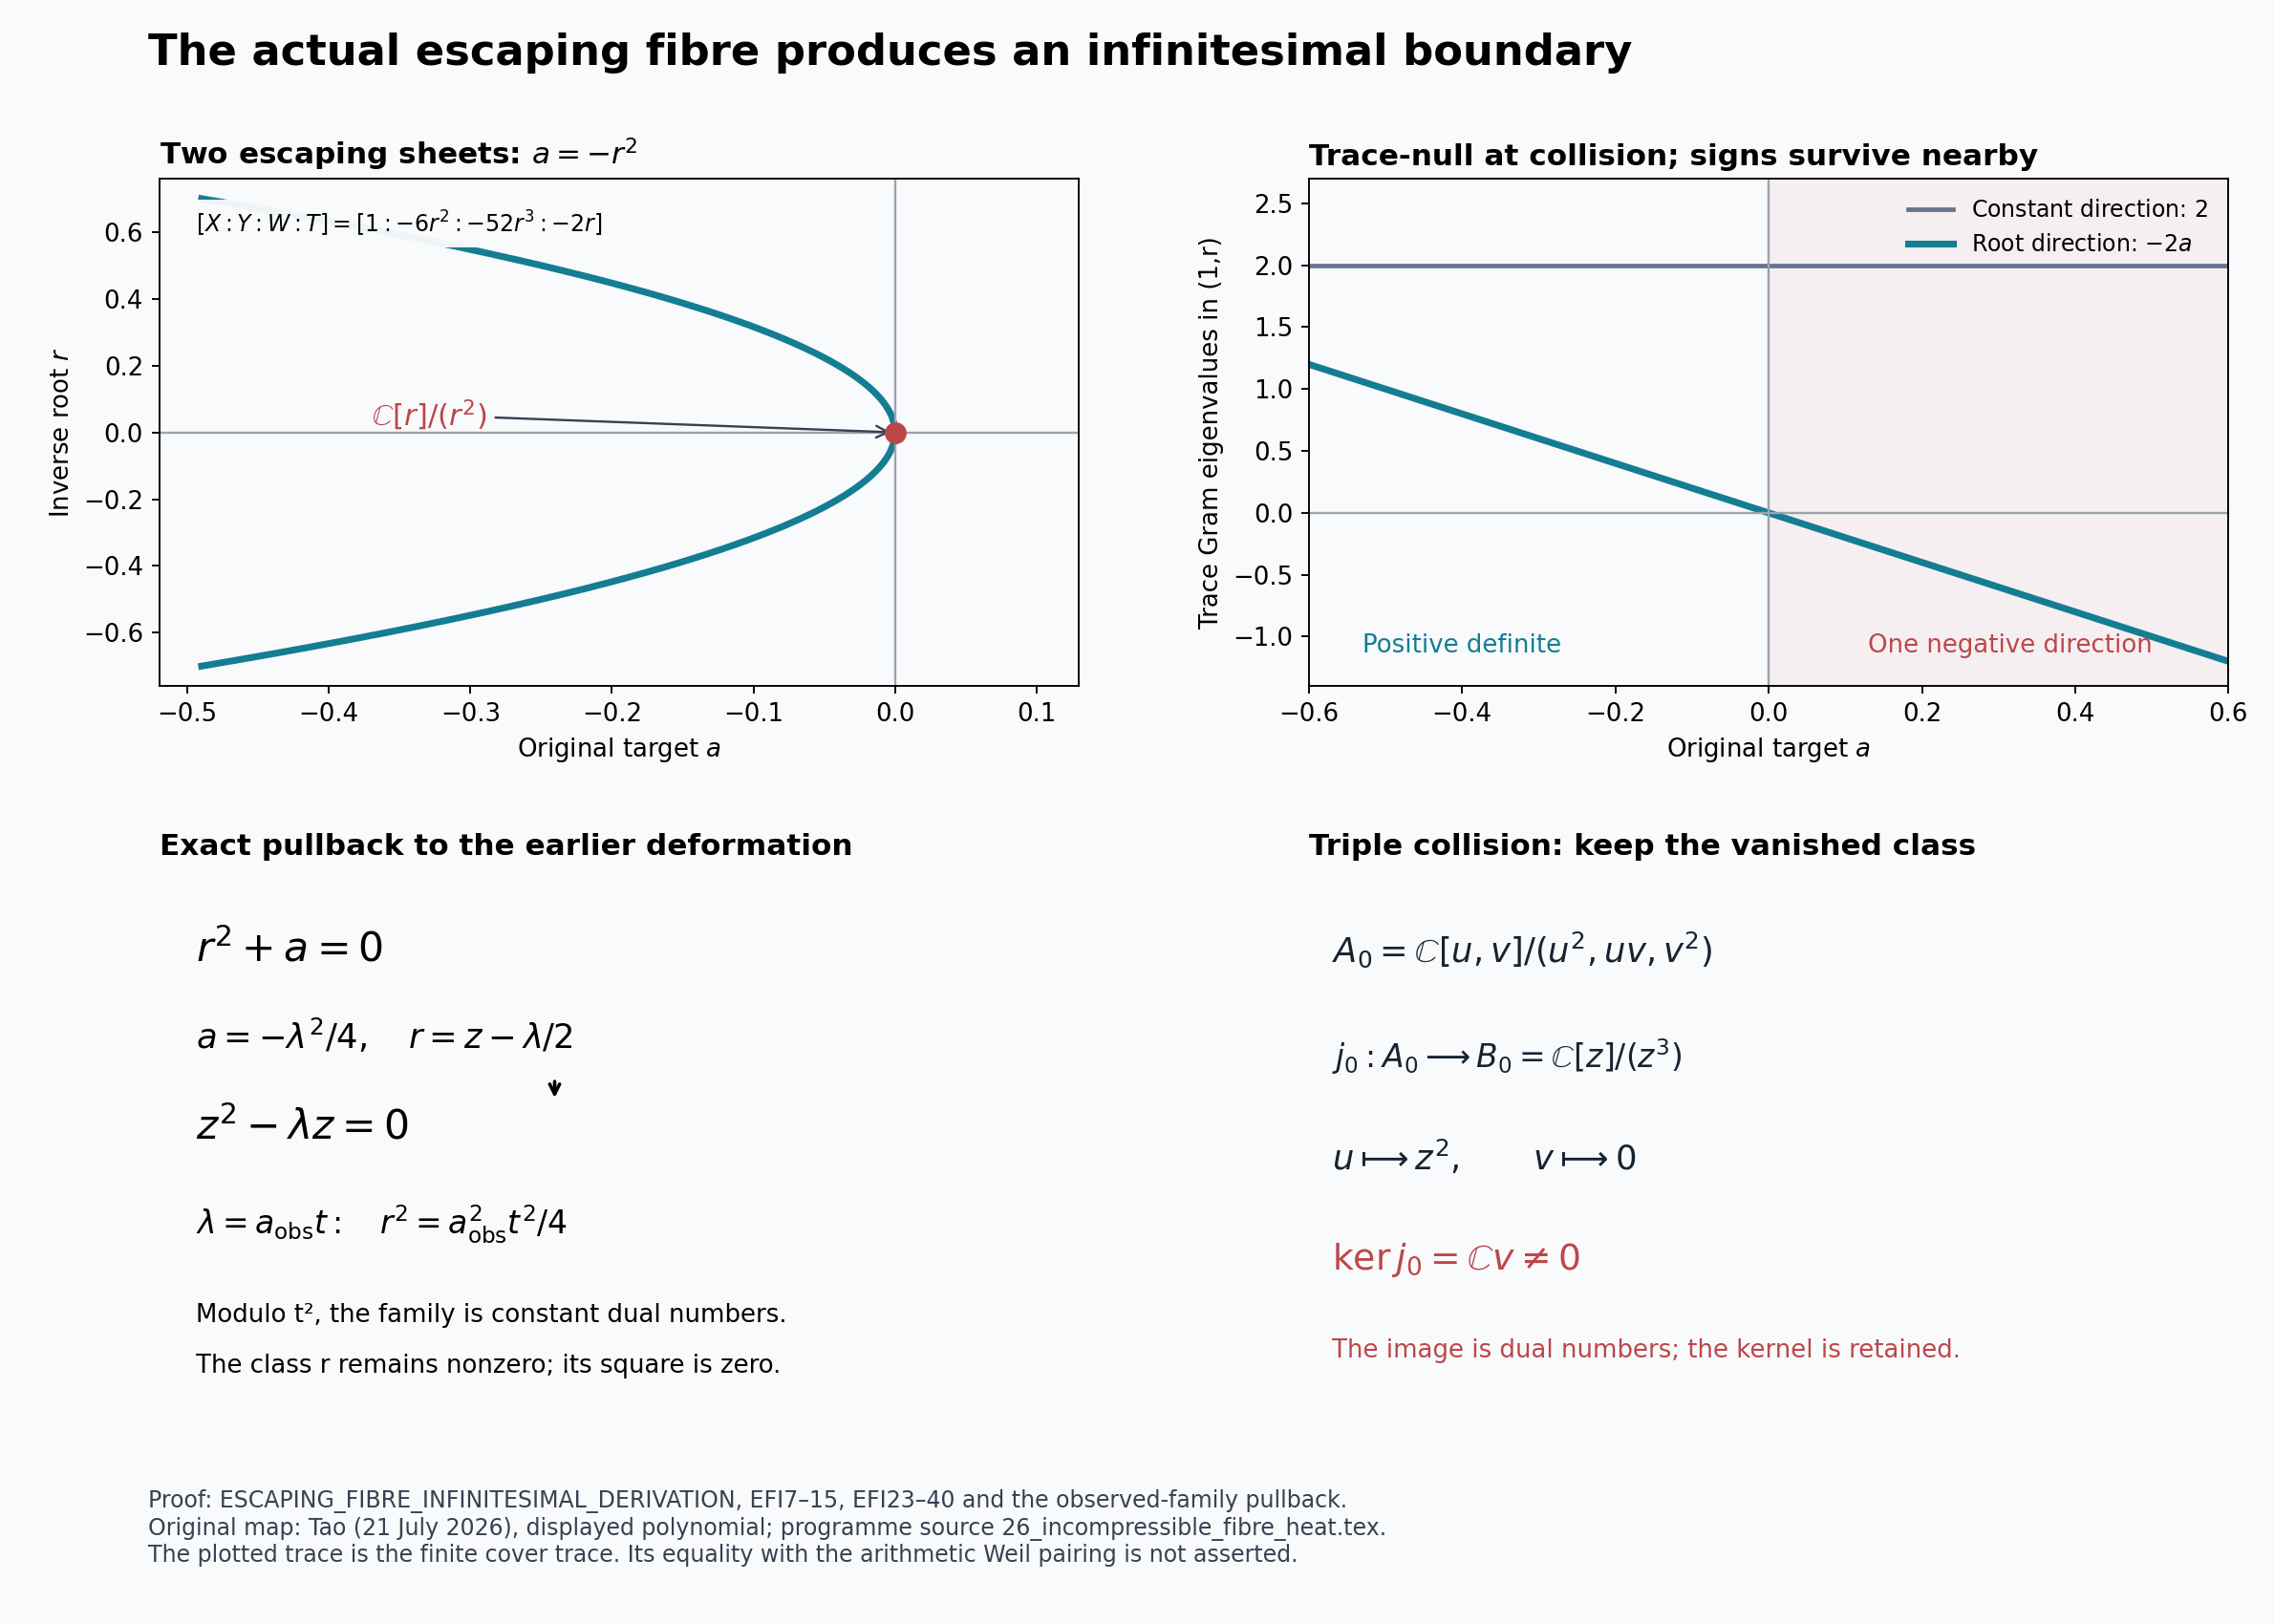
\includegraphics[keepaspectratio,alt={The exact cover a=-r² and finite trace eigenvalues; the observed-family pullback retains the collision generator. The triple graph map retains its kernel. Proof: EFI7--EFI15, EFI23--EFI40, EFI51--EFI68.}]{figures/25_escaping_trace.png}}
\caption{The exact cover a=-r² and finite trace eigenvalues; the
observed-family pullback retains the collision generator. The triple
graph map retains its kernel. Proof: EFI7--EFI15, EFI23--EFI40,
EFI51--EFI68.}
\end{figure}

\clearpage

\section{Infinitesimal vanishing, retained currents, and support-valued
positivity}\label{infinitesimal-vanishing-retained-currents-and-support-valued-positivity}

22 September 2026. This note computes the several different vanishing
statements at the observed collision, the complete signs that survive,
and the exact class of corrections capable of changing them. The
calculations retain the original observation, metric, Hermitian summand,
amplitude multiplier, and full support algebra. No off-line zero of the
Riemann zeta function is asserted to exist.

The incoming public programme proofs are
\href{https://github.com/KokunoYumeto/zeta-function-research-reader/blob/c9df443d9e1df000dfbb083943f97197e746eb08/workbenches/splitzero-tandem/branches/identity-absorber-square/OBSERVED_COLLISION.md}{\emph{The
observed infinitesimal collision and the full arithmetic operator},
OC1--OC17};
\href{https://github.com/KokunoYumeto/zeta-function-research-reader/blob/c9df443d9e1df000dfbb083943f97197e746eb08/workbenches/splitzero-tandem/branches/identity-absorber-square/OBSERVED_SUPPORT_PROPAGATION.md}{\emph{Observed
support at the shifted nilpotent collision}, OSP1--OSP42}; and
\href{https://github.com/KokunoYumeto/zeta-function-research-reader/blob/c9df443d9e1df000dfbb083943f97197e746eb08/workbenches/splitzero-tandem/branches/identity-absorber-square/OBSERVED_COTANGENT_FROBENIUS.md}{\emph{Cotangent
and Frobenius calculations for the observed collision}, OCF1--OCF23 and
OIF1--OIF36}. The additional complete local dependencies are
\href{https://github.com/KokunoYumeto/zeta-function-research-reader/blob/173dbc6ed5a03235dbe7654f928f3692107db39b/workbenches/splitzero-tandem/branches/tau-zero-prime-positivity/FULL_SUPPORT_RECONSTRUCTION_DERIVATION.md}{full-support
reconstruction proof}, FSR1--FSR36;
\href{https://github.com/KokunoYumeto/zeta-function-research-reader/blob/173dbc6ed5a03235dbe7654f928f3692107db39b/workbenches/splitzero-tandem/branches/tau-zero-prime-positivity/WEIL_PACKET_DERIVATION.md}{finite
Weil packet proof}, WP1--WP57; and
\href{https://github.com/KokunoYumeto/zeta-function-research-reader/blob/173dbc6ed5a03235dbe7654f928f3692107db39b/workbenches/splitzero-tandem/branches/tau-zero-prime-positivity/WEIL_PACKET_ANALYTIC_DERIVATION.md}{analytic
Weil packet proof}, WA1--WA30. Their complete sources accompany this
derivation; no public link is asserted for an unpublished dependency.
The cited proofs retain their original human citations. This is a
further finite derivation and an application of the already proved
analytic identity WA24, not a replacement for its analytic proof.

\subsection{1. Original operators and the
collision}\label{original-operators-and-the-collision}

Keep the original source data and metric from OC1--OC3: \[
M=C+R,\quad C=C^\dagger,\quad R=\epsilon fe^\dagger,
\quad e^\dagger e=f^\dagger f=1,\quad e^\dagger f=0,\quad\epsilon>0,
\] \[
J=G_N^{-1}\Lambda^*Q_B^{1/2},\quad
Q_B=(\Lambda G_N^{-1}\Lambda^*)^{-1},\quad J^\dagger J=I_B,
\quad C_B=J^\dagger CJ=C_B^*.
\tag{ISP1}
\] Here the original arithmetic quotient, cutoff, and observation remain
those of OC1: \(q=(k+1)^2\), \(k\ge17\), \(k\equiv1\pmod4\),
\(q-1\le N\le2q\), and the original surjection \(\Lambda:E\to B\). The
star is the adjoint in the Euclidean coordinates supplied by the
isometry \(J\); it does not change the original metric.

Write \[
u=J^\dagger e,\quad v=J^\dagger f,\quad
a=u^*u,\quad r=u^*v,\quad d=v^*v,\quad
\Delta=ad-|r|^2>0.
\] The measured area statement in OC3 supplies this strict inequality.
Define \[
g=u/\sqrt a,\qquad
h=\frac{v-(r/a)u}{\sqrt{\Delta/a}},\qquad
b=\epsilon\sqrt\Delta>0,\qquad P=gg^*+hh^*.
\tag{ISP2}
\] The numerator defining \(h\) has inner product zero with \(u\),
because \(u^*v-(r/a)u^*u=0\). Its squared norm is
\(d-|r|^2/a=\Delta/a\). Thus \(g,h\) are an orthonormal pair and \(P\)
is their orthogonal projector.

The exact observed family is \[
F_B(s)=(\epsilon v+su)u^*,\qquad
M_B(s)=C_B+F_B(s),\qquad
\lambda(s)=as+\epsilon r.
\tag{ISP3}
\] Direct multiplication gives \(F_B(s)^2=\lambda(s)F_B(s)\). On the
original orthogonal plane \(S=\operatorname{im}P\), and on its
orthogonal complement \(H\), respectively, it is \[
F_B(s)|_S=\begin{pmatrix}\lambda(s)&0\\b&0\end{pmatrix},
\qquad F_B(s)|_H=0.
\tag{ISP4}
\] At the collision parameter \[
s_*=-\epsilon r/a,
\quad N=F_B(s_*)=\epsilon\bigl(v-(r/a)u\bigr)u^*=bhg^*,
\quad N^2=0,\quad Ng=bh\ne0.
\tag{ISP5}
\] The map \(\mathbb C[\eta]/(\eta^2)\to\operatorname{End}(B)\),
\(1\mapsto I_B\), \(\eta\mapsto N\), is injective. Indeed a relation
\(cI_B+\ell N=0\) applied to \(h\) gives \(c=0\), and then applied to
\(g\) gives \(\ell b=0\), hence \(\ell=0\). Its image is exactly the
generated algebra. The supported version sends its unit to \(P\) and has
the same proof on \(S\).

\subsection{2. Exactly what vanishes}\label{exactly-what-vanishes}

For the isolated nilpotent operator, for every scalar \(t\), \[
\operatorname{tr}(N^j)=0\quad(j\ge1),\qquad
\det(I_B-tN)=1,\qquad
(I_B-tN)^{-1}=I_B+tN.
\tag{ISP6}
\] In the basis \(g,h\), \(N\) is strictly triangular, and is zero on
\(H\). This proves the trace and determinant assertions; multiplication
proves the inverse. A marked matrix element retains the exact term \[
x^*((I_B-tN)^{-1}-I_B)y
=tb(x^*h)(g^*y).
\tag{ISP7}
\] For \(x=h,y=g\), this term is \(tb\), which is nonzero when
\(t\ne0\). Vanishing of the isolated trace series therefore has an
explicit kernel and a nonzero receiver.

The family algebra itself is \[
\mathcal A=\mathbb C[t,z]/(z(z-at)),\qquad t=s-s_*.
\] The invertible change \(\xi=z-at/2\), with inverse \(z=\xi+at/2\),
gives \[
z(z-at)=\xi^2-a^2t^2/4.
\tag{ISP8}
\] Over \(\mathbb C[t]/(t^2)\), this is an isomorphism with the constant
dual-number family, and it reduces to the identity on the fibre \(t=0\).
Thus its first-order deformation class vanishes. Over
\(\mathbb C[t]/(t^3)\), the trace discriminant in the basis \(1,z\)
equals \(a^2t^2\ne0\); the constant dual-number family's trace
discriminant is zero. To compute it, multiplication by \(z\) has trace
\(at\), and multiplication by \(z^2=at z\) has trace \(a^2t^2\). The
trace matrix is therefore
\(\left(\begin{smallmatrix}2&at\\at&a^2t^2\end{smallmatrix}\right)\),
with determinant \(a^2t^2\). An invertible basis change multiplies its
determinant by a unit square. Hence it cannot turn this nonzero
discriminant into zero. The first nontrivial order is exactly two.

The original operator representation and its metric retain additional
information. Work now over \(\mathbb C[t]/(t^2)\), and put \[
K=\frac{a}{2b}gh^*,\qquad T=I_B+tK,\qquad T^{-1}=I_B-tK.
\] Since \([K,N]=(a/2)(gg^*-hh^*)\), direct multiplication proves \[
F_B(s_*+t)=TNT^{-1}+\frac{at}{2}P,
\] \[
T^{-1}M_B(s_*+t)T
=C_B+N+t\left([C_B,K]+\frac a2P\right).
\tag{ISP9}
\] Here \(C_B\) remains the original operator on all of \(B\); it need
not preserve \(S\). These formulas follow by expanding products and
using \(t^2=0\). If the formal parameter is given the real involution
\(t^*=t\), then \[
T^*T=I_B+t(K+K^*).
\tag{ISP10}
\] The coefficient \(K+K^*\) is nonzero, because \((K+K^*)h=(a/(2b))g\).
Thus this coordinate trivialization is not unitary for the original
metric. Equations ISP9--ISP10 retain the exact operator and metric
changes attached to the vanishing deformation class.

There is also a choice-dependent Frobenius vanishing. Over a torsionfree
integral collision ring \(D_p=K_p[\eta]/\eta^2\) with the coefficient
Frobenius specified in OIF33, every lift is \[
\Phi_c(\eta)=pc\eta,\qquad c\in K_p.
\tag{ISP11}
\] To verify this, write an image as \(A+B\eta\). Its square is zero, so
the coefficient domain forces \(A=0\). Its reduction must equal
\(\eta^p=0\), forcing \(B\in pK_p\); the converse is immediate. The
corrected lift has \(c=0\), so kills \(\eta\), whereas the earlier
multiplicative lift has \(c=1\) and sends it to \(p\eta\ne0\). The same
underlying nilpotent algebra therefore does not determine this Frobenius
vanishing without the specified lift.

\subsection{3. The full arithmetic determinant does not vanish
infinitesimally}\label{the-full-arithmetic-determinant-does-not-vanish-infinitesimally}

Keep \(C_B\) in the characteristic polynomial, and let \(n=\dim B\).
Rank-one determinant expansion gives \[
\det(\zeta I_B-C_B-N)
=\det(\zeta I_B-C_B)
-b\,g^*\operatorname{adj}(\zeta I_B-C_B)h.
\tag{ISP12}
\] For a proof, expand the determinant column by column. Every term
containing at least two columns from \(bhg^*\) vanishes because those
columns are proportional to \(h\). The terms containing exactly one such
column sum to the displayed adjugate contraction, with the minus sign
from the subtracted perturbation. This proof is a polynomial identity
and does not require an inverse.

In particular, the isolated identity \(\det(I-tN)=1\) does not remove
the second term of ISP12. On the plane, the concrete Hermitian choice
\(C_B|_S=\left(\begin{smallmatrix}0&c\\c&0\end{smallmatrix}\right)\),
\(c\in\mathbb R\setminus\{0\}\), gives \[
\det(\zeta I_S-C_B|_S-N|_S)=\zeta^2-c(c+b),
\qquad \det(\zeta I_S-C_B|_S)=\zeta^2-c^2.
\tag{ISP13}
\] This example disproves an inference from nilpotence alone; it is not
substituted for the native \(C_B\).

For the actual family, define \[
p_*(\zeta)=\det(\zeta I_B-M_B(s_*)),\qquad
q_*(\zeta)=u^*\operatorname{adj}(\zeta I_B-M_B(s_*))u.
\] The same polynomial expansion proves, exactly for every \(t\), \[
p_{s_*+t}(\zeta)=p_*(\zeta)-tq_*(\zeta).
\tag{ISP14}
\] Moreover \(q_*\) has degree \(n-1\) and leading coefficient
\(u^*u=a>0\): the adjugate of \(\zeta I_B-M_B(s_*)\) has leading
coefficient \(\zeta^{n-1}I_B\). Consequently the full characteristic
polynomial has a nonzero first derivative in the original parameter,
even though the abstract algebra deformation class in ISP8 vanishes.
Equivalently,
\(\operatorname{tr}M_B(s_*+t)=\operatorname{tr}M_B(s_*)+at\). These
statements concern the actual original family.

\subsection{4. The signed current survives with both
signs}\label{the-signed-current-survives-with-both-signs}

Use exactly the programme convention \[
W_B(s)=i(M_B(s)-M_B(s)^*).
\] The retained Hermitian term cancels in this particular difference
because \(C_B=C_B^*\). It remains in ISP12--ISP14. Direct conjugate
transposition of ISP4 gives \[
W_B(s)|_S=
\begin{pmatrix}-2\operatorname{Im}\lambda(s)&-ib\\ib&0\end{pmatrix},
\qquad W_B(s)|_H=0.
\tag{ISP15}
\] At the infinitesimal collision, \[
W_*:=W_B(s_*)=i(N-N^*),\qquad
W_*^2=b^2P,
\] \[
W_*\frac{g+ih}{\sqrt2}=b\frac{g+ih}{\sqrt2},\qquad
W_*\frac{g-ih}{\sqrt2}=-b\frac{g-ih}{\sqrt2}.
\tag{ISP16}
\] These follow by multiplying the two-by-two matrix, or by using
\(Ng=bh,Nh=0,N^*h=bg,N^*g=0\). Its inertia on \(B\) is \((1,1,n-2)\).
For \(y=c_g g+c_hh+y_H\), \[
y^*W_*y=2b\operatorname{Im}(\overline{c_g}c_h).
\tag{ISP17}
\] Thus the two unit eigenvectors in ISP16 have values \(+b\) and
\(-b\), not zero.

The current correction from the original parameter \(s=0\) is exactly \[
W_*-W_B(0)=2\epsilon\operatorname{Im}(r)gg^*.
\tag{ISP18}
\] For every complex parameter \(s\), the determinant of its active
matrix in ISP15 is \(-b^2<0\). Consequently that rank-one displacement
cannot make the current positive semidefinite. Along the real
displacement \(s=s_*+t\), \(t\in\mathbb R\), the full current is exactly
constant, \(W_B(s_*+t)=W_*\), because \(\lambda(s_*+t)=at\) is real.

\subsection{5. All Hermitian corrections on the current
plane}\label{all-hermitian-corrections-on-the-current-plane}

Write an arbitrary Hermitian correction on \(S\) as \[
D=\begin{pmatrix}\alpha&c\\\overline c&\delta\end{pmatrix},
\qquad\alpha,\delta\in\mathbb R,\quad c\in\mathbb C.
\] Then the complete set of corrections giving a nonnegative form is \[
\boxed{W_*+D\succeq0
\quad\Longleftrightarrow\quad
\alpha\ge0,\ \delta\ge0,\ \alpha\delta\ge|c-ib|^2.}
\tag{ISP19}
\] For necessity evaluate on \(g,h\), obtaining the diagonal
inequalities, and use the nonnegative determinant. For sufficiency, when
\(\alpha>0\), complete the square: \[
\alpha\left|x+\frac{c-ib}{\alpha}y\right|^2
+\left(\delta-\frac{|c-ib|^2}{\alpha}\right)|y|^2\ge0.
\] When \(\alpha=0\), the determinant inequality forces \(c-ib=0\), and
the form is \(\delta|y|^2\). This proves every boundary case as well as
the positive-definite case.

In particular, an orthogonal-support correction \(tP\),
\(t\in\mathbb R\), gives positivity exactly for \(t\ge b\). A correction
supported only on \(gg^*\), or only on \(hh^*\), never suffices. The
equality \(e^2=e\) by itself supplies no scalar coefficient \(t\); ISP19
states the exact correction needed by the operator it would act on.

The analogous complete classification for a larger support space is as
follows. Let \(X,Z\) be finite-dimensional Hermitian spaces and let \[
\mathcal Q=\begin{pmatrix}H&A\\A^*&D\end{pmatrix}
\quad\text{on }X\oplus Z,
\qquad H=H^*,\quad D=D^*.
\] Let \(D^+\) be the operator equal to the reciprocal of each nonzero
eigenvalue of \(D\) and zero on its kernel. Then \[
\boxed{\mathcal Q\succeq0\quad\Longleftrightarrow\quad
D\succeq0,\quad A(\ker D)=0,\quad H-AD^+A^*\succeq0.}
\tag{ISP20}
\] To prove necessity, first restrict to \(Z\). For \(z_0\in\ker D\),
the value on \((x,tz_0)\) is \(x^*Hx+2\operatorname{Re}(t x^*Az_0)\).
Its nonnegativity for every complex \(t\) forces \(Az_0=0\). Thus
\(A^*x\) belongs to \((\ker D)^\perp=\operatorname{im}D\). For all
\(x,z\), exact multiplication now gives \[
\langle(x,z),\mathcal Q(x,z)\rangle
=x^*(H-AD^+A^*)x
+(z+D^+A^*x)^*D(z+D^+A^*x).
\tag{ISP21}
\] Set \(z=-D^+A^*x\) for the last necessary inequality. Conversely
ISP21 proves positivity from the three displayed conditions. This proof
constructs the minimizing support coordinate and includes singular
\(D\).

For a fixed Hermitian correction \(R\) to the old block, replace \(H\)
in ISP20 by \(H+R\); the result classifies every such corrected
extension. Adding independent support coordinates and mixed blocks while
leaving \(H\) unchanged cannot remove an old negative value: it is still
the value on \((x,0)\). Indeed minimizing over the added positive
coordinates subtracts \(AD^+A^*\), exactly as ISP21 records.

\subsection{6. Full support and every positive scalar
trace}\label{full-support-and-every-positive-scalar-trace}

Retain the finite bounded distributive lattice \(L\), the actual
semiring \(G_L(R)\), and its supported zero \(e_L\), with \((e_L)=Z_L\)
prime when \(R\) is a domain. This is prior programme mathematics, not a
new result here. The contracted multiplicative algebra is the proved
product \[
\Gamma_L=\mathbb C[(G_L(R),\times)]/([\tau_L])
\cong C_L\times D_R,
\quad C_L=\mathbb C[(L,\wedge)]/([0_L]).
\tag{ISP22}
\] In this algebra \([e_L]\) is the identity of the \(C_L\) factor. It
is a multiplicative idempotent, not the square-zero operator \(N\) of
ISP5. The latter comes from the separate, explicitly specified
deformation/observation receiver. The exact role of the former in the
following coefficient extension is multiplication by the support
identity.

FSR11--FSR14 give \[
C_L=\bigoplus_{a\in L\setminus\{0\}}\mathbb CE_a,
\quad E_aE_b=\delta_{ab}E_a,\quad E_a^*=E_a,
\quad\sum_aE_a=1_{C_L}.
\tag{ISP23}
\] For completeness, the characters are
\(\eta_a([\lambda])=1_{a\le\lambda}\); their incidence matrix is
triangular with diagonal one, hence invertible. Its inverse gives
\(E_a=\sum_{\lambda\le a}\mu(\lambda,a)[\lambda]\). Applying every
character proves the stated multiplication and unit identities.

Every positive complex-linear scalar functional on \(C_L\) is uniquely
\[
\ell\Bigl(\sum_ac_aE_a\Bigr)=\sum_at_ac_a,
\qquad t_a\ge0.
\tag{ISP24}
\] Indeed \(E_a=E_a^*E_a\) forces \(\ell(E_a)\ge0\); conversely the
displayed coefficients give \(\ell(v^*v)=\sum_at_a|v_a|^2\ge0\). It is
faithful on positive elements precisely when every \(t_a>0\).

Extend the actual current coefficientwise to \(B_L=C_L\otimes B\),
retaining \(1\otimes C_B\) in its full arithmetic operator. Its
support-valued form is \[
\mathcal W_L(x,y)=\sum_aE_a x_a^*W_*y_a,
\qquad x=\sum_aE_a\otimes x_a.
\tag{ISP25}
\] For every \(a\) with \(t_a>0\), the exact vector \[
x_a^-=E_a\otimes(g-ih)/\sqrt2
\quad\text{has}\quad
\mathcal W_L(x_a^-,x_a^-)=-bE_a,
\qquad\ell\mathcal W_L(x_a^-,x_a^-)=-bt_a<0.
\tag{ISP26}
\] Thus every nonzero positive functional retains a negative direction
for this form. If exactly \(r\) of the weights are positive and
\(d_L=|L|-1\), its scalar inertia is \[
(r,r,(n-2)r+n(d_L-r)).
\tag{ISP27}
\] This follows by using the two eigenvectors in ISP16 and a basis of
\(H\) in every sector; the sectors of weight zero contribute their
entire \(n\)-dimensional space to the radical.

The same proof applied to the full finite Weil pairing FSR28, whose
scalar inertia is \((2,2,4m-4)\), gives \[
\operatorname{inertia}(\ell\mathbb B_L)
=(2r,2r,(4m-4)r+4m(d_L-r)).
\tag{ISP28}
\] In particular, the regular trace has all weights one. Boolean branch
traces select only join-irreducible sectors and put zero weights on the
remaining mixed sectors; zero observation there does not prove zero full
form. For \(L=\mathbb B^2\), the mixed projector \(w=[1]-[a]-[b]\) obeys
\(w^2=w\ne0\), both branch traces kill it, and FSR34--FSR35 give the
exact value \(-2m w\) on the specified mixed negative packet.

\subsection{7. Exact maps from the collision current to a quartet
packet}\label{exact-maps-from-the-collision-current-to-a-quartet-packet}

This section constructs a finite comparison without identifying it with
the native period observation. Let \(\rho=1/2+\delta+i\gamma\),
\(0<\delta<1/2\), \(\gamma>2\), and use the four distinct points \[
(\alpha_1,\alpha_2,\alpha_3,\alpha_4)
=(\rho,1-\overline\rho,\overline\rho,1-\rho).
\] For \(m\ge1\), let \(d(s)=\prod_i(s-\alpha_i)\), \(h(s)=d(s)^m\),
\(E_h=\mathbb C[s]/(h)\), and let \(e_i\) be the full primary
idempotents. Let \(U=M_{j_h(v)}\) be the original amplitude unit, with
its full Taylor coefficients and nonzero values \(v(\alpha_i)\). Let
\(a_h=\operatorname{ev}U:E_h\to\mathbb C^4\). The finite pairing is \[
B_h(x,y)=m\bigl(\overline{(a_hx)_2}(a_hy)_1+
\overline{(a_hx)_1}(a_hy)_2+
\overline{(a_hx)_4}(a_hy)_3+
\overline{(a_hx)_3}(a_hy)_4\bigr).
\tag{ISP29}
\] These algebraic data can be defined for arbitrary such points and an
arbitrary specified unit; they do not assert a zeta zero.

Define the typed injective linear map \[
\mathcal I:S\longrightarrow E_h,
\quad c_gg+c_hh\longmapsto
\sqrt{b/m}\,U^{-1}(c_ge_1-ic_he_2).
\tag{ISP30}
\] Applying \(a_h\) gives \(\sqrt{b/m}(c_g,-ic_h,0,0)\), so injectivity
follows. Substitution in ISP29 gives the exact isometry \[
B_h(\mathcal I x,\mathcal I y)=x^*W_*y\qquad(x,y\in S).
\tag{ISP31}
\] Explicitly the right side is
\(-ib\overline{x_g}y_h+ib\overline{x_h}y_g\), and the left side has the
same two coefficients. This is an isometry of Hermitian forms, whose
signs are indefinite; it is not asserted to preserve the original
positive norm.

There is also a nilpotent operator on the complete packet, including all
its jets: \[
\mathcal N_h(x)=-ib\,(a_hx)_1 U^{-1}e_2.
\tag{ISP32}
\] Since \((a_hU^{-1}e_2)_1=0\), it has square zero. It is nonzero on
\(U^{-1}e_1\), and direct substitution proves \[
\mathcal N_h\mathcal I=\mathcal I N|_S.
\tag{ISP33}
\] This comparison preserves the constant \(b\), its complex phase, and
the original \(U\). It sends the radical \(J_h=(d)/(d^m)\) to zero by
the formula for \(a_h\); every radical jet remains in the domain and in
\(U\). Extending ISP30--ISP33 by \(C_L\otimes-\) gives the identical
maps in every support sector. The construction is explicit and depends
on the chosen quartet; equality with the original period receiver has
not been asserted or assumed.

\subsection{8. Interpolation removes endpoint terms without changing any
packet
jet}\label{interpolation-removes-endpoint-terms-without-changing-any-packet-jet}

Since none of the four points is \(0\) or \(1\), \(h(0)h(1)\ne0\). For a
polynomial \(q\), set \[
\boxed{\mathcal R_hq(s)=q(s)-h(s)
\left((1-s)\frac{q(0)}{h(0)}+s\frac{q(1)}{h(1)}\right).}
\tag{ISP34}
\] This is a linear polynomial map. Substitution at the two endpoints
gives \[
\mathcal R_hq(0)=\mathcal R_hq(1)=0,
\qquad\mathcal R_hq\equiv q\pmod h.
\tag{ISP35}
\] The latter congruence preserves the derivatives of every order
\(0,\ldots,m-1\) at every \(\alpha_i\), because \(h\) has order \(m\)
there. Conversely divisibility by \(h\) is exactly the kernel of the
complete quartet jet map, by successive division by the four distinct
linear factors. Therefore every original packet class, including every
nilpotent jet and the entire action of \(U\), is retained by this map.

Let \(s_h:E_h\to\mathbb C[s]\) select the unique representative of
degree below \(4m\), as supplied by monic polynomial division. The
composite \[
\widetilde s_h=\mathcal R_hs_h:
E_h\longrightarrow s(s-1)\mathbb C[s]
\tag{ISP36}
\] is a linear section of polynomial reduction modulo \(h\), with degree
at most \(4m+1\). Its image has dimension \(4m\), and every class has
exactly the stated lift. In particular this endpoint condition does not
constrain any quartet jet.

The same statement holds for arbitrary specified finite endpoint orders.
For \(K\ge1\), put \(b_K(s)=s^K(s-1)^K\). It is a unit in \(E_h\),
because each \(b_K(\alpha_i)\ne0\). An explicit inverse is obtained by
the finite Taylor reciprocal in each factor \(\mathbb C[t_i]/(t_i^m)\),
followed by the primary idempotent inverse of the jet map. Consequently
\[
\widetilde s_{h,K}(x)=b_K\,s_h\bigl([b_K]^{-1}x\bigr)
\tag{ISP37}
\] is a linear section of reduction modulo \(h\) whose values vanish to
order at least \(K\) at both \(0\) and \(1\). Multiplication followed by
reduction proves the section identity exactly. This constructs the
connecting map for every finite endpoint jet constraint.

\subsection{9. Consequence for the explicit formula and zero-prime
corrections}\label{consequence-for-the-explicit-formula-and-zero-prime-corrections}

The following application concerns the programme's counterfactual zeta
packet used in WP1--WP4 and WA1--WA2: its four specified points have
exact zero order \(m\) for \(g=2\xi\), so \(v=g/h\) is entire and has
nonzero values there. This is the established test of an off-line
packet; it is not an existence claim.

For two polynomials \(q_1,q_2\), use exactly \[
q^\#(s)=\overline{q(1-\overline s)},\qquad
A_{q_1,q_2}(s)=q_1^\#(s)q_2(s)v(s)^2.
\tag{ISP38}
\] Let \(\widetilde q_i=\mathcal R_hq_i\). Equations ISP35 and WP21
prove that the original full primary amplitude jets of
\(\widetilde q_iv\) and \(q_iv\) agree. Furthermore \[
A_{\widetilde q_1,\widetilde q_2}(0)
=A_{\widetilde q_1,\widetilde q_2}(1)=0.
\tag{ISP39}
\] Indeed the factor \(\widetilde q_2\) vanishes at both endpoints. This
conclusion also follows by evaluating the reflected first factor; no
positivity inference is used.

Take the full-jet negative class \[
x_-=U^{-1}(e_1-e_2),\qquad
\widetilde q_- =\widetilde s_h(x_-).
\tag{ISP40}
\] Its four amplitude values are exactly \((1,-1,0,0)\), hence \[
B_h([\widetilde q_-],[\widetilde q_-])=-2m.
\tag{ISP41}
\] Its Fourier-coordinate polynomial is
\(\widetilde P_-(z)=\widetilde q_-(1/2+iz)\); define
\(F_-(z)=\widetilde P_-(z)v(1/2+iz)\), \[
K_-(t)=|F_-(t)|^2,\qquad
k_-(u)=\frac1{2\pi}\int_{\mathbb R}K_-(t)e^{itu}\,dt.
\] WA9--WA16 apply to every polynomial, so the increased degree in ISP36
changes their constants but not the proved admissibility, exponential
strip decay, or absolute convergence. Substitution into the full
analytic identity WA24, using ISP39, gives \[
\boxed{-2m=
\frac1{2\pi}\int_{\mathbb R}|F_-(t)|^2
\left(\operatorname{Re}\psi(\tfrac14+\tfrac{it}{2})-\log\pi\right)dt
-\sum_{n\ge2}\frac{\Lambda_{\rm ar}(n)}{\sqrt n}
\bigl(k_-(\log n)+k_-(-\log n)\bigr).}
\tag{ISP42}
\] This is the exact endpoint-free arithmetic expression for that
packet, with every sign and transform convention retained. It does not
prove that this packet exists for zeta, and does not prove nonnegativity
of the arithmetic expression.

More generally let \(\mathcal E(q)\) be the vector of any fixed finite
list of derivatives at \(0,1\), and let \(D=D^*\) be any matrix on that
vector space. Every correction \[
\mathcal D(q_1,q_2)=\mathcal E(q_1)^*D\mathcal E(q_2)
\tag{ISP43}
\] vanishes on the image of ISP37 for sufficiently large \(K\). Yet that
image surjects onto every packet jet and contains the negative class
ISP40. The same conclusion holds if \(\mathcal E\) takes the endpoint
jets of \(qv\): multiplication by the entire function \(v\) preserves
the required vanishing orders. Thus no correction factoring solely
through finitely many endpoint evaluations or endpoint derivatives makes
this packet form positive. This is a classification of that class of
corrections, not an assumption that all effects of the zero prime belong
to it.

In full support, choose any sector \(E_a\) and lift the polynomial as
\(E_a\widetilde q_-\). Its exact support-valued form is \(-2mE_a\),
while all the specified endpoint jets are zero. A positive scalar trace
with weight \(t_a>0\) reads \(-2mt_a<0\), by ISP24. Mixed sectors obey
the same calculation, including sectors omitted by every separate
Boolean branch.

The proved zero-prime structure therefore changes the spectrum and
enlarges the retained coefficient and observation spaces, as FSR1--FSR22
specify. A corrected analytic formula must supply its actual
distribution or operator on these spaces. The results above already
settle three concrete possibilities: nilpotence alone does not kill the
observed current; coefficientwise full-support extension does not change
its surviving signs; and a finite endpoint correction cannot erase the
explicit negative quartet test. The spaces and maps exposed by these
statements are ISP20--ISP21, ISP23--ISP28, and ISP34--ISP43. They retain
the objects on which a further arithmetic correction must act.

\subsection{10. The endpoint pairing also has a computable
sign}\label{the-endpoint-pairing-also-has-a-computable-sign}

For this quartet polynomial, \[
h(0)=h(1)=\bigl(|\rho|^2|1-\rho|^2\bigr)^m>0,
\qquad v(0)=v(1)=c_0:=1/h(0)>0.
\] The first equality follows by grouping the conjugate factors and
using the reflection permutation of the four roots. The second uses the
exact convention \(g(0)=g(1)=1\) of WA1. Hence for endpoint vectors
\(e(q)=(q(0),q(1))\), the pole pairing itself is \[
\begin{aligned}
A_{q_1,q_2}(0)+A_{q_1,q_2}(1)
&=c_0^2\bigl(\overline{q_1(1)}q_2(0)+\overline{q_1(0)}q_2(1)\bigr)\\
&=e(q_1)^*\,c_0^2\begin{pmatrix}0&1\\1&0\end{pmatrix}e(q_2).
\end{aligned}
\tag{ISP44}
\] Thus the pole contribution by itself has one positive and one
negative endpoint direction. Evaluation onto \(\mathbb C^2\) is
surjective by the polynomial \((1-s)c+sd\), so both directions occur.
This computes the actual contribution already present in WA24; it does
not assign an unproved coefficient to the additional prime \((e_L)\).
The section ISP36 kills both of these directions while preserving every
packet jet.

\subsection{11. Exact finite
verification}\label{exact-finite-verification}

The reproducible script
\texttt{check\_\allowbreak{}infinitesimal\_\allowbreak{}support\_\allowbreak{}positivity.\allowbreak{}py} passed 38 exact
symbolic checks, recorded in
\texttt{INFINITESIMAL\_\allowbreak{}SUPPORT\_\allowbreak{}POSITIVITY\_\allowbreak{}CHECKS.\allowbreak{}json}. The checks
include the nilpotent/current identities, both signed eigenvectors, the
first-order conjugation with a Hermitian matrix coupling the current
plane to its complement, the full characteristic polynomial, the
current-to-packet isometry and intertwiner, every retained jet in a
multiplicity-two quartet example, endpoint vanishing through order two
in the higher-order section, the singular-block square-completion
identity, and the eight exact module/metric identities of ISP46--ISP53.
The calculations use exact rational and symbolic coefficients. The
finite sample points are not asserted to be zeta zeros. These checks
support the displayed algebraic calculations; they do not replace the
general proofs above or assert a new analytic positivity theorem.

\subsection{12. The positive escaping trace and the original observed
metric}\label{the-positive-escaping-trace-and-the-original-observed-metric}

The escaping-family isomorphism EFI52--EFI55 uses the exact base map
\(a_{\rm esc}=-\lambda^2/4\) and coordinate
\(r_{\rm esc}=z_{\rm obs}-\lambda/2\). Along the real displacement
\(s-s_*\), the observed coefficient \(\lambda=a(s-s_*)\) is real. Its
algebra multiplication trace in the basis \(1,z_{\rm obs}\) is \[
G_{\mathrm{tr}}(\lambda)=\begin{pmatrix}2&\lambda\\\lambda&\lambda^2\end{pmatrix}.
\tag{ISP45}
\] Indeed \(z_{\rm obs}^2=\lambda z_{\rm obs}\), multiplication by
\(z_{\rm obs}\) has trace \(\lambda\), and multiplication by its square
has trace \(\lambda^2\), while the identity has trace two. The centered
coordinate \(r_{\rm esc}=z_{\rm obs}-\lambda/2\) gives the congruent
matrix \(\operatorname{diag}(2,\lambda^2/2)\). Thus this form is
positive definite for real \(\lambda\ne0\), and has one-dimensional
radical at zero. The following calculation gives its exact relationship
to the original metric and current.

Write \(z=z_{\rm obs}\) for the retained observed generator. Retain
\(S=\operatorname{span}\{g,h\}\) with its original orthonormal frame,
and \(b=\epsilon\sqrt\Delta>0\). The supported receiver is \[
\rho_\lambda:\mathbb C[z]/(z^2-\lambda z)\longrightarrow\operatorname{End}(S),
\quad 1\mapsto I_S,\quad z\mapsto F_\lambda=
\begin{pmatrix}\lambda&0\\b&0\end{pmatrix}.
\tag{ISP46}
\] It is a homomorphism because \(F_\lambda^2=\lambda F_\lambda\). It is
injective: a linear relation \(cI_S+dF_\lambda=0\) applied to \(h\)
gives \(c=0\), and applied to \(g\) then gives \(db=0\). The cyclic
module map from its regular representation to \(S\) is \[
T_\lambda:\mathbb C[z]/(z^2-\lambda z)\longrightarrow S,
\quad 1\mapsto g,\quad z\mapsto\lambda g+bh,
\quad [T_\lambda]_{(1,z),(g,h)}=
\begin{pmatrix}1&\lambda\\0&b\end{pmatrix}.
\tag{ISP47}
\] Its determinant is \(b\ne0\). Direct multiplication proves
\(F_\lambda T_\lambda=T_\lambda M_z\), where
\(M_z=\left(\begin{smallmatrix}0&0\\1&\lambda\end{smallmatrix}\right)\).
Thus regular multiplication and the supported receiver have the same
ordinary traces.

The algebra involution used in ISP45 fixes \(z\) when \(\lambda\) is
real. Its image is not fixed by the original matrix adjoint: \[
\rho_\lambda(z^*)-\rho_\lambda(z)^*
=F_\lambda-F_\lambda^*=-iW_*,
\quad W_*=\begin{pmatrix}0&-ib\\ib&0\end{pmatrix}.
\tag{ISP48}
\] The equality follows by conjugate transposition. It is nonzero for
every real \(\lambda\), including zero. Thus the exact map relating the
forms is a faithful algebra receiver with this specified adjoint defect.

There are three retained Hermitian forms on the same two-dimensional
coordinate space. The algebra multiplication trace gives ISP45. Pulling
back the original vector metric through ISP47 gives \[
G_{\mathrm{vec}}=T_\lambda^*T_\lambda
=\begin{pmatrix}1&\lambda\\\lambda&\lambda^2+b^2\end{pmatrix}.
\tag{ISP49}
\] Pulling back the matrix Hilbert--Schmidt metric through ISP46 gives
\[
G_{\mathrm{HS}}=
\begin{pmatrix}
\operatorname{Tr}(I_S)&\operatorname{Tr}(F_\lambda)\\
\operatorname{Tr}(F_\lambda^*)&\operatorname{Tr}(F_\lambda^*F_\lambda)
\end{pmatrix}
=\begin{pmatrix}2&\lambda\\\lambda&\lambda^2+b^2\end{pmatrix}.
\tag{ISP50}
\] Every entry follows by multiplying the displayed matrix
\(F_\lambda\). In particular \[
G_{\mathrm{HS}}-G_{\mathrm{tr}}
=\begin{pmatrix}0&0\\0&b^2\end{pmatrix},
\qquad \|\rho_0(z)\|_{\mathrm{HS}}^2=b^2>0.
\tag{ISP51}
\] The trace-null generator at collision has a nonzero, exactly measured
operator norm. The supported unit in ISP46 has rank two. Using instead
the full unital receiver \(1\mapsto I_B\) changes the upper-left entry
of ISP50 to \(\dim B\); it does not change its other three entries.

The trace pairing makes multiplication by the real generator
self-adjoint, as matrix multiplication verifies: \[
G_{\mathrm{tr}}M_z=M_z^*G_{\mathrm{tr}}.
\] For the positive matrix metric the exact defect is instead \[
G_{\mathrm{HS}}M_z-M_z^*G_{\mathrm{HS}}
=\begin{pmatrix}0&-b^2\\b^2&0\end{pmatrix}.
\tag{ISP52}
\] This is obtained by subtracting the two products, with no limiting
argument. Thus the extra positive term in ISP51 has a specified effect
on multiplication adjoints; it cannot be added while asserting unchanged
adjoint compatibility.

Finally, transporting the trace form itself to the original vector plane
gives \[
Q_\lambda=(T_\lambda^{-1})^*G_{\mathrm{tr}}T_\lambda^{-1}
=\begin{pmatrix}2&-\lambda/b\\-\lambda/b&\lambda^2/b^2\end{pmatrix},
\quad\det Q_\lambda=\lambda^2/b^2.
\tag{ISP53}
\] The inverse
\(T_\lambda^{-1}=\left(\begin{smallmatrix}1&-\lambda/b\\0&1/b\end{smallmatrix}\right)\)
proves the formula by multiplication. This positive metric for
\(\lambda\ne0\) makes \(F_\lambda\) self-adjoint; at the collision it
becomes degenerate and kills \(h\). There cannot be a positive definite
metric making the nonzero \(N=bhg^*\) self-adjoint: that would imply
\(\langle Nx,Nx\rangle=\langle x,N^2x\rangle=0\) for every \(x\),
forcing \(N=0\). The explicitly constructed degenerate metric ISP53 is
the retained limiting object, while the original positive metric and the
current \(W_*\) remain unchanged.

The Hermitian summand \(C_B\) of the full arithmetic operator remains in
ISP12--ISP14. The present algebra comparison concerns \(F_\lambda\), and
makes no commutation assertion about \(C_B\) or identification of the
trace metric with the classical Weil form.

\begin{figure}
\centering
\pandocbounded{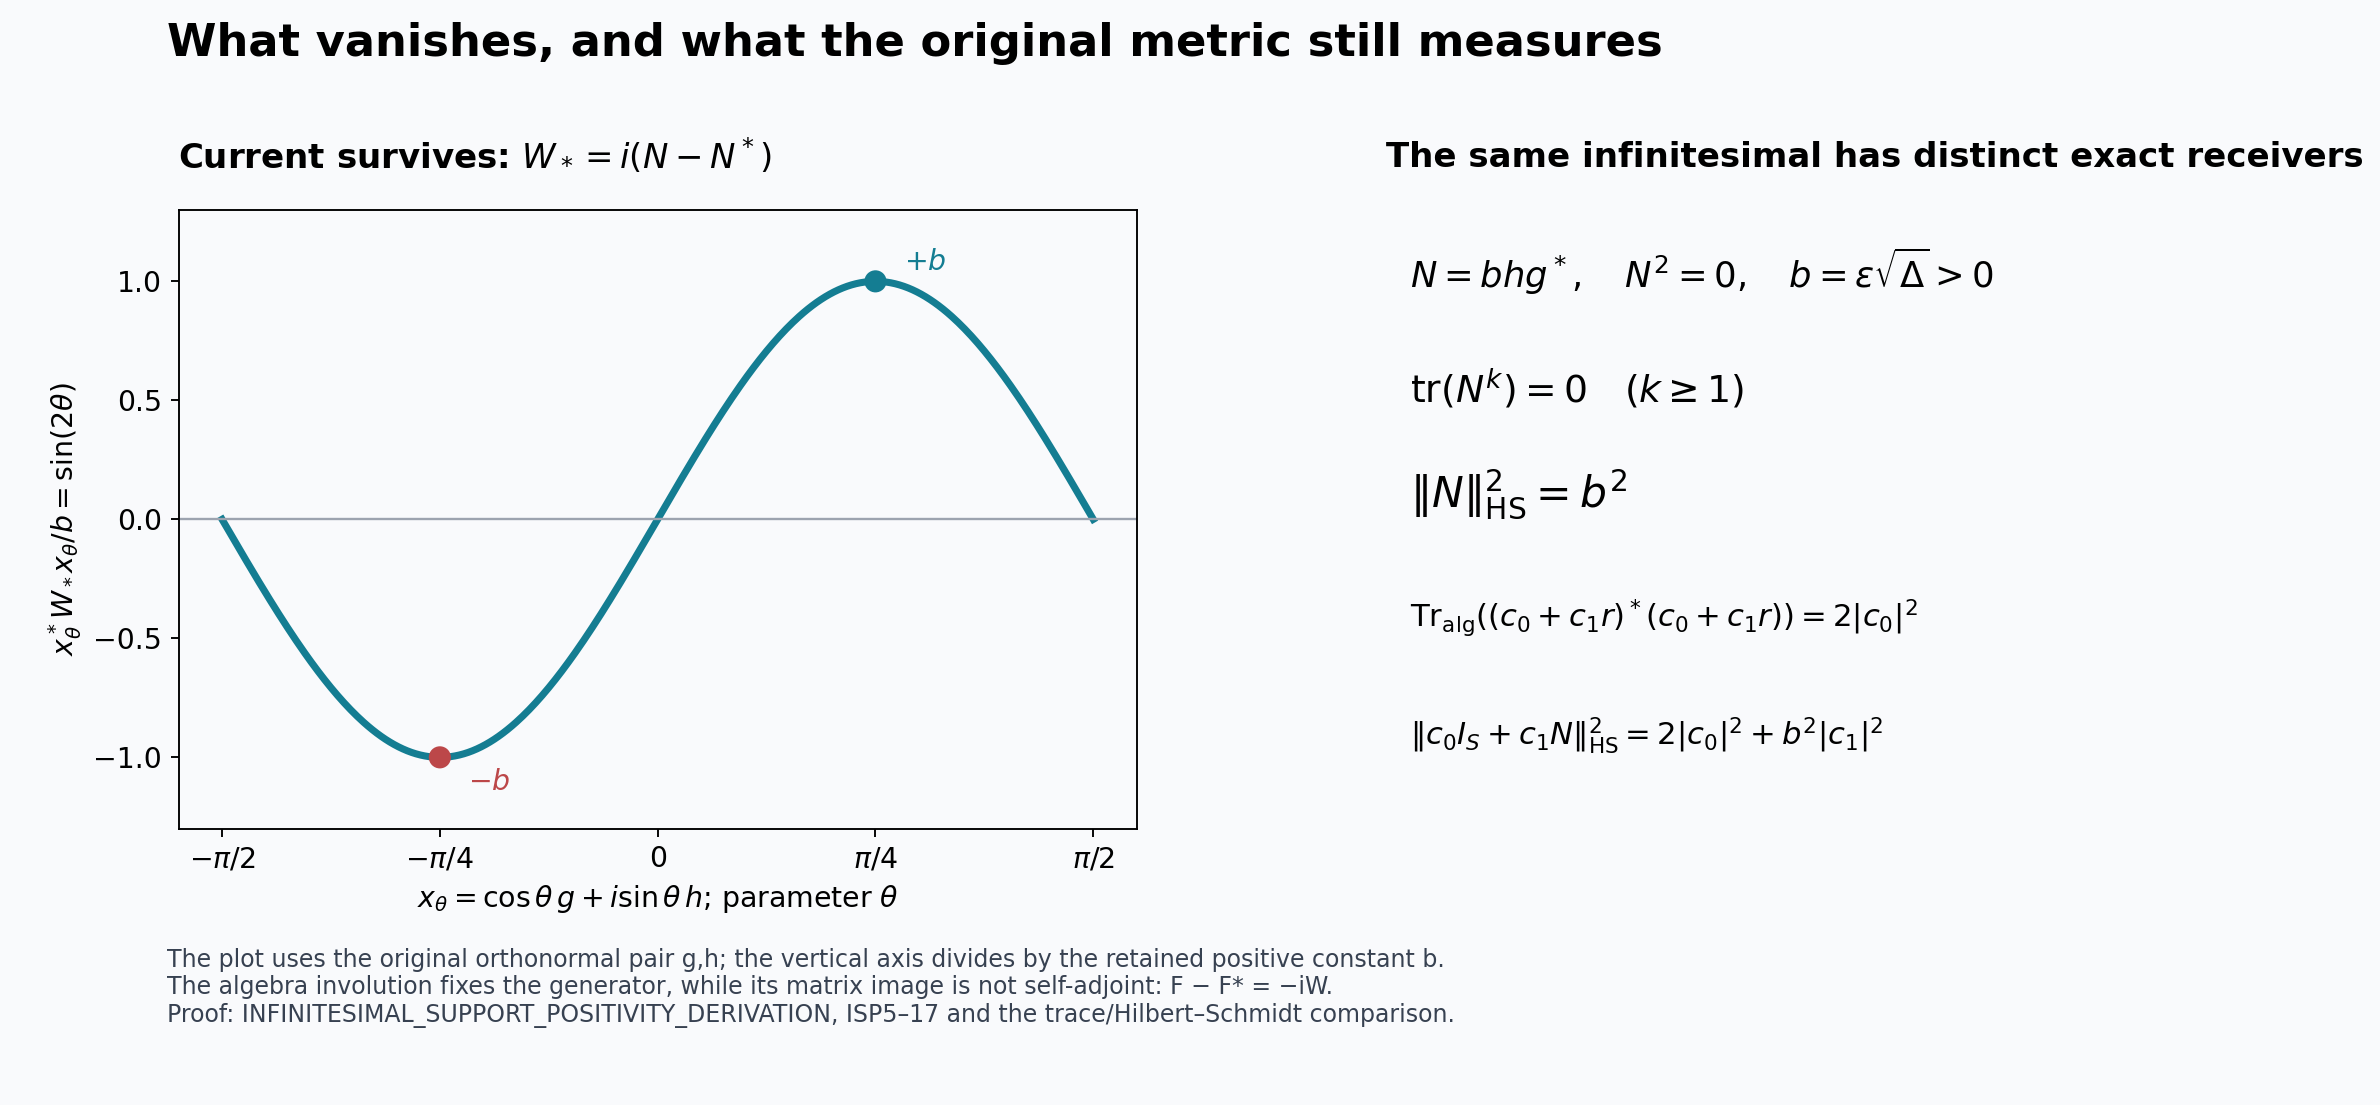
\includegraphics[keepaspectratio,alt={The same nonzero infinitesimal has zero algebraic trace and nonzero matrix norm; its current has both signs in the original metric. Proof: ISP5--ISP6, ISP18--ISP20, ISP45--ISP53.}]{figures/26_infinitesimal_forms.png}}
\caption{The same nonzero infinitesimal has zero algebraic trace and
nonzero matrix norm; its current has both signs in the original metric.
Proof: ISP5--ISP6, ISP18--ISP20, ISP45--ISP53.}
\end{figure}

\clearpage

\section{The logarithmic arithmetic distribution of the
separated-support zeta
sheet}\label{the-logarithmic-arithmetic-distribution-of-the-separated-support-zeta-sheet}

This calculation uses the actual interpolation in the programme's
\emph{Secondary Note on Split-Zero Globalization}, canonical source
PUBUNIT-B1A260A5E731EA568C353AA4, equations under
\texttt{def:\allowbreak{}hurwitz-\allowbreak{}specialization},
\texttt{thm:\allowbreak{}universal-\allowbreak{}taylor-\allowbreak{}deformation},
\texttt{thm:\allowbreak{}arithmetic-\allowbreak{}kernels-\allowbreak{}riemann}, and
\texttt{cor:\allowbreak{}first-\allowbreak{}log-\allowbreak{}jet-\allowbreak{}explicit}. It also uses \emph{Split-Zero
Support Repair}, \texttt{some\ considerrations.\allowbreak{}tex}, sections
``Conservative ideal and zeta side'' and ``Shifted zeta deformation''.
These are prior programme results. The supported-zero prime is also a
prior result of Paper 1, attributed by the user to Gemini Pro 2.5. The
calculation below derives the signed arithmetic distribution that
replaces the prime-power distribution for this particular separated
sheet. It does not assign an arbitrary finite norm to the supported-zero
prime.

\subsection{NL1. The original scalar maps and the actual analytic
family}\label{nl1.-the-original-scalar-maps-and-the-actual-analytic-family}

Let \(R=\mathbb Z\), and let \(G(R)=R\sqcup\{\tau\}\). Addition and
multiplication on supported elements are their ring operations;
\(\tau+x=x\) and \(\tau x=\tau\). Write \(e=0_R\), so \(e\ne\tau\),
\(e^2=e\), and \(er=e\) for every supported \(r\). The two maps \[
p:G(R)\to R,\quad p(r)=r,\ p(\tau)=0,
\qquad
\chi:G(R)\to\mathbb B,\quad \chi(r)=1,\ \chi(\tau)=0
\tag{NL1}
\] preserve both operations and units, directly by these laws. The prime
ideal \((e)=\{\tau,e\}\) is \(p^{-1}(0)\); its complement consists of
nonzero integers and is multiplicatively closed. This proves its
primality without identifying its generator with the semiring zero.

The separated residue map \(G(\mathbb Z)\to G(\mathbb Z/n\mathbb Z)\),
obtained by reducing the supported amplitude and keeping \(\tau\), has
target cardinality \(n+1\). This holds also for \(n=1\): the zero ring
has a supported zero and the distinct \(\tau\). Composing with amplitude
gives \(\mathbb Z/n\mathbb Z\), of cardinality \(n\). Thus the two
defined sums are \[
F_0(s)=\sum_{n\ge1}n^{-s}=\zeta(s),\qquad
F_1(s)=\sum_{n\ge1}(n+1)^{-s}=\zeta(s)-1.
\tag{NL2}
\] Their interpolation is \[
F_t(s)=\sum_{n\ge1}(n+t)^{-s}=\zeta(s,1+t),\qquad t\ge0,\quad\Re s>1.
\tag{NL3}
\] Here \(t\) is a real shift parameter, not the semiring element
\(\tau\). The equality with Hurwitz zeta is the defining series with its
index translated; compare the original TeX formulas at
\href{https://dlmf.nist.gov/25.11.E1}{DLMF 25.11.1} and
\href{https://dlmf.nist.gov/25.11.E3}{25.11.3}.

The prime \((e)\) cannot be inserted into the old ideal Euler product
with a positive finite multiplicative norm extending the integer ideal
norm. Indeed \((e)I_{(n)}=(e)\); a multiplicative norm \(h\) would
satisfy \(h((e))=n h((e))\), so \(h((e))=0\) for \(n=2\). This equality
specifies the obstruction. The separated residue sum (NL3) is a
different, already defined analytic receiver of support. Its logarithmic
distribution is now calculated in full.

\subsection{NL2. A convergent expansion with every multiplicative
interaction
retained}\label{nl2.-a-convergent-expansion-with-every-multiplicative-interaction-retained}

Put \[
b=1+t,\qquad r_n=\frac{n+t}{1+t}\quad(n\ge2),\qquad
H_t(s)=\sum_{n\ge2}r_n^{-s}.
\tag{NL4}
\] Every \(r_n>1\), and \[
F_t(s)=b^{-s}(1+H_t(s)).
\tag{NL5}
\] There exists \(\sigma_0>1\) with \(H_t(\sigma_0)<1\). To prove this,
fix any \(\sigma_1>1\). The terms \(r_n^{-\sigma}\) tend to zero as
\(\sigma\to\infty\), and for \(\sigma\ge\sigma_1\) they are dominated by
the summable sequence \(r_n^{-\sigma_1}\). Dominated convergence gives
\(H_t(\sigma)\to0\).

On every closed half-plane \(\Re s\ge\sigma_0\) with
\(H_t(\sigma_0)<1\), the series \[
\log F_t(s)=-s\log b+
\sum_{k\ge1}\frac{(-1)^{k+1}}{k}
\sum_{n_1,\ldots,n_k\ge2}
(r_{n_1}\cdots r_{n_k})^{-s}
\tag{NL6}
\] uses the holomorphic logarithm of \(1+H_t\) defined by its power
series. Its absolute sum is at most
\(\sum_{k\ge1}H_t(\sigma_0)^k/k<\infty\). Differentiation is locally
uniformly justified: for a slightly smaller abscissa still exceeding 1
and with \(H_t<1\), \[
J_t(\sigma)=\sum_{n\ge2}(\log r_n)r_n^{-\sigma}<\infty,
\] and the absolute sum of the differentiated length terms of length
\(k\), after the factor \(1/k\), is \(J_t(\sigma)H_t(\sigma)^{k-1}\).
Summing this geometric bound proves \[
-\frac{F_t'(s)}{F_t(s)}
=\log b+
\sum_{k\ge1}\frac{(-1)^{k+1}}{k}
\sum_{n_1,\ldots,n_k\ge2}
\log(r_{n_1}\cdots r_{n_k})
(r_{n_1}\cdots r_{n_k})^{-s}.
\tag{NL7}
\] No factor indexed by an ordinary prime has been assumed.

Define the signed measure on \([0,\infty)\) \[
\nu_t=(\log b)\delta_0+
\sum_{k\ge1}\frac{(-1)^{k+1}}k
\sum_{n_1,\ldots,n_k\ge2}
\ell(n_1,\ldots,n_k)\delta_{\ell(n_1,\ldots,n_k)},
\quad
\ell(n_1,\ldots,n_k)=\sum_i\log r_{n_i}.
\tag{NL8}
\] It is locally finite: if \(\ell\le M\), then \(k\le M/\log r_2\), and
every \(r_{n_i}\le e^M\), leaving finitely many tuples. Equal lengths
are added with their exact signed multiplicities. The same bound proving
(NL7) gives \(\int e^{-\sigma\ell}|d\nu_t|<\infty\) in the stated right
half-plane. Its Laplace transform is exactly \(-F_t'/F_t\).

\subsection{NL3. An explicit negative arithmetic atom at the separated
endpoint}\label{nl3.-an-explicit-negative-arithmetic-atom-at-the-separated-endpoint}

At \(t=1\), \(b=2\), \(r_n=(n+1)/2\), and \[
H_1(4)=\sum_{m\ge3}(2/m)^4
\le\frac{16}{81}+\int_3^\infty16x^{-4}\,dx
=\frac{32}{81}<1.
\tag{NL9}
\] Thus (NL7) holds, in particular, for \(\Re s\ge4\), with the
convergence estimate just proved. There is a positive atom \[
\nu_1(\{\log(3/2)\})=\log(3/2).
\tag{NL10}
\] Only the one-term tuple \(n_1=2\) has that length: a tuple of at
least two terms has product at least \((3/2)^2\).

There is also the exact negative atom \[
\boxed{\nu_1(\{\log(9/4)\})=-\log(3/2).}
\tag{NL11}
\] For a one-term tuple, \((n+1)/2=9/4\) would give \(n=7/2\),
impossible. A tuple of at least three terms has product at least
\(27/8>9/4\). For two terms both factors are at least \(3/2\), so
equality forces both to be \(3/2\), that is, the single ordered tuple
\((2,2)\). Its coefficient in (NL8) is
\(-\tfrac12\log(9/4)=-\log(3/2)\). This proves (NL11) with no
truncation.

Consequently the logarithmic arithmetic distribution for the actual
separated sheet is signed. The original von Mangoldt distribution,
\(\sum_{n\ge2}\Lambda(n)\delta_{\log n}\), cannot be reused for this
sheet. The negative atom alone is not a negative value of the full Weil
form: the gamma, divisor, reflection-defect, and boundary terms of a
complete contour identity must also be retained. It is an exact
arithmetic coefficient that such an identity must contain.

\subsection{NL4. The first infinitesimal is nonzero and contains mixed
prime
data}\label{nl4.-the-first-infinitesimal-is-nonzero-and-contains-mixed-prime-data}

For \(|t|<1\), the binomial series gives, locally uniformly for
\(\Re s>1\), \[
F_t(s)=\zeta(s)-t\,s\zeta(s+1)+O(t^2).
\tag{NL12}
\] For completeness, fix a compact set of \(s\) and a radius \(r<1\).
The Taylor remainder in \((1+t/n)^{-s}\) is bounded by a constant times
\(|t|^2/n^2\), uniformly on that compact set; after multiplication by
\(n^{-s}\) it is summable. This proves the asserted termwise expansion
and its holomorphic derivatives.

The Euler product of \(\zeta\), used only at \(t=0\), gives \[
Q(s)=\frac{\zeta(s+1)}{\zeta(s)}
=\sum_{n\ge1}\alpha(n)n^{-s},\qquad
\alpha(1)=1,\quad
\alpha(n)=(-1)^{\omega(n)}\frac{\prod_{p\mid n}(p-1)}{n}.
\tag{NL13}
\] Indeed the local series is \[
\frac{1-p^{-s}}{1-p^{-s-1}}
=1-\sum_{j\ge1}\frac{p-1}{p^j}p^{-js}.
\] Its absolute product converges for \(\Re s>1\); multiplying the
series proves (NL13). Thus \[
\left.\partial_t\log F_t(s)\right|_{t=0}=-sQ(s),
\qquad
\left.\partial_t\left(-\frac{F_t'}{F_t}\right)\right|_{t=0}
=Q(s)+sQ'(s)
=\sum_{n\ge1}\alpha(n)(1-s\log n)n^{-s}.
\tag{NL14}
\] The derivative series is absolutely convergent on compact subsets of
\(\Re s>1\), since \(|\alpha(n)|\le1\) and
\(\sum(1+\log n)n^{-\sigma}<\infty\). For real \(s>1\), \(sQ(s)>0\), so
the first deformation of \(\log F_t\) does not vanish. This
infinitesimal is not the first-order-trivial node deformation from the
observed collision.

Equation (NL14) is equivalently the Laplace transform of the locally
finite distribution \[
\dot\nu_0=
\sum_{n\ge1}\alpha(n)
\bigl(\delta_{\log n}-(\log n)\delta'_{\log n}\bigr).
\tag{NL15}
\] Here \(\langle\delta'_\ell,f\rangle=-f'(\ell)\), so its Laplace
transform is \(s e^{-s\ell}\). This fixes the derivative sign in (NL15).

The dot also denotes the actual distributional derivative of (NL8), not
only a matching transform. On a fixed compact length interval and for
\(0\le t\le1\), the inequalities \(r_2(t)\ge3/2\) and
\(r_n(t)\ge(n+1)/2\) give a uniform finite bound on the tuples which can
enter. Differentiating their smooth moving atoms therefore defines the
derivative on every compactly supported smooth test. For weighted
Laplace tests, \(|\partial_t\log r_n|\le1\). A tuple of length \(k\) has
length derivative bounded by \(k\); differentiating its coefficient and
its exponential introduces at most one further factor \(k\), together
with its original length. On a sufficiently far right half-plane,
uniformly in a neighborhood of zero, the sums are bounded by geometric
series of the forms \(\sum k B^k\) and \(\sum k D B^{k-1}\), with
\(B<1\) and \(D<\infty\) as above. Thus Laplace transformation commutes
with differentiation. At zero all tuple lengths are logs of positive
integers. The resulting distribution has the form
\(\sum_n(a_n\delta_{\log n}+b_n\delta'_{\log n})\). These coefficients
are uniquely determined by its Laplace transform: multiply the
difference of two such transforms by the exponential of its least
remaining length and let the real argument tend to infinity; the leading
polynomial of degree at most one must be zero, and induction removes
every length. The exponentially weighted convergence just proved bounds
the remaining tail in each step. Comparing with (NL14) proves exactly
\(a_n=\alpha(n)\), \(b_n=-(\log n)\alpha(n)\), as in (NL15).

For distinct primes \(p,q\), \[
\alpha(pq)=\frac{(p-1)(q-1)}{pq}\ne0.
\tag{NL16}
\] These are supported at products of distinct primes, whereas the
original von Mangoldt coefficients vanish there. The deformation
therefore has explicitly nonzero mixed-prime terms already at first
order; they cannot be removed by keeping only a modified weight at each
prime power.

\subsection{NL5. Full finite support and exact
specialization}\label{nl5.-full-finite-support-and-exact-specialization}

For a finite bounded distributive support lattice \(L\), the actual set
is \[
G_L(R)=\{(0,\lambda):\lambda\in L\}\cup\{(r,1_L):r\in R\}.
\tag{NL17}
\] Let \(c=|L|-1\). Its separated residue over \(\mathbb Z/n\mathbb Z\)
has \(n+c\) elements: \(n\) supported top elements and \(|L|-1\) lower
support elements. Hence its scalar cardinality receiver is \[
F_c(s)=\sum_{n\ge1}(n+c)^{-s}
=\zeta(s)-\sum_{n=1}^{c}n^{-s}.
\tag{NL18}
\] This proves exactly how (NL3) receives the full support count. It
does not identify different support labels with one another in \(G_L\).
The cardinality map forgets that distinction; the full meet-algebra
coefficients and their primitive idempotents remain separate in the
programme's full-support reconstruction. Formula (NL8) applies with
\(t=c\) to the count receiver. All logarithmic product tuples, including
their collisions in the length variable, are retained.

\subsection{NL6. Consequence for the positivity
calculation}\label{nl6.-consequence-for-the-positivity-calculation}

There are three exact facts to carry forward. First, the supported-zero
prime remains a nontrivial prime of \(G(\mathbb Z)\); no positive finite
multiplicative ideal norm extending the old norm can give it an ordinary
new Euler factor. Second, the programme already supplies a different
analytic receiver, the separated quotient-size interpolation (NL3),
whose logarithmic derivative is (NL7), with the explicit signed atom
(NL11). Third, its infinitesimal variation is (NL14), not zero. A
corrected explicit formula for this receiver must use these arithmetic
terms and its own completed divisor. The exact escaping-fibre trace and
observed-operator current are calculated in the accompanying
derivations; equality with a Weil form requires the actual map, not an
identification of their names.

The two primitive-defect source files in folders 3 and 4 are
byte-identical (SHA256
\texttt{2f3289f6\allowbreak{}a04105d3\allowbreak{}f15fe5f7\allowbreak{}c36dde28\allowbreak{}6515e61f\allowbreak{}465caf15\allowbreak{}82f9808e\allowbreak{}19f3d2f7}).
Their negative augmentation retains the kernel of a scalar cancellation.
That same instruction is followed here: the full signed length
distribution (NL8) and mixed-prime distribution (NL15) are retained
rather than discarded when an ordinary Euler presentation fails.

\begin{figure}
\centering
\pandocbounded{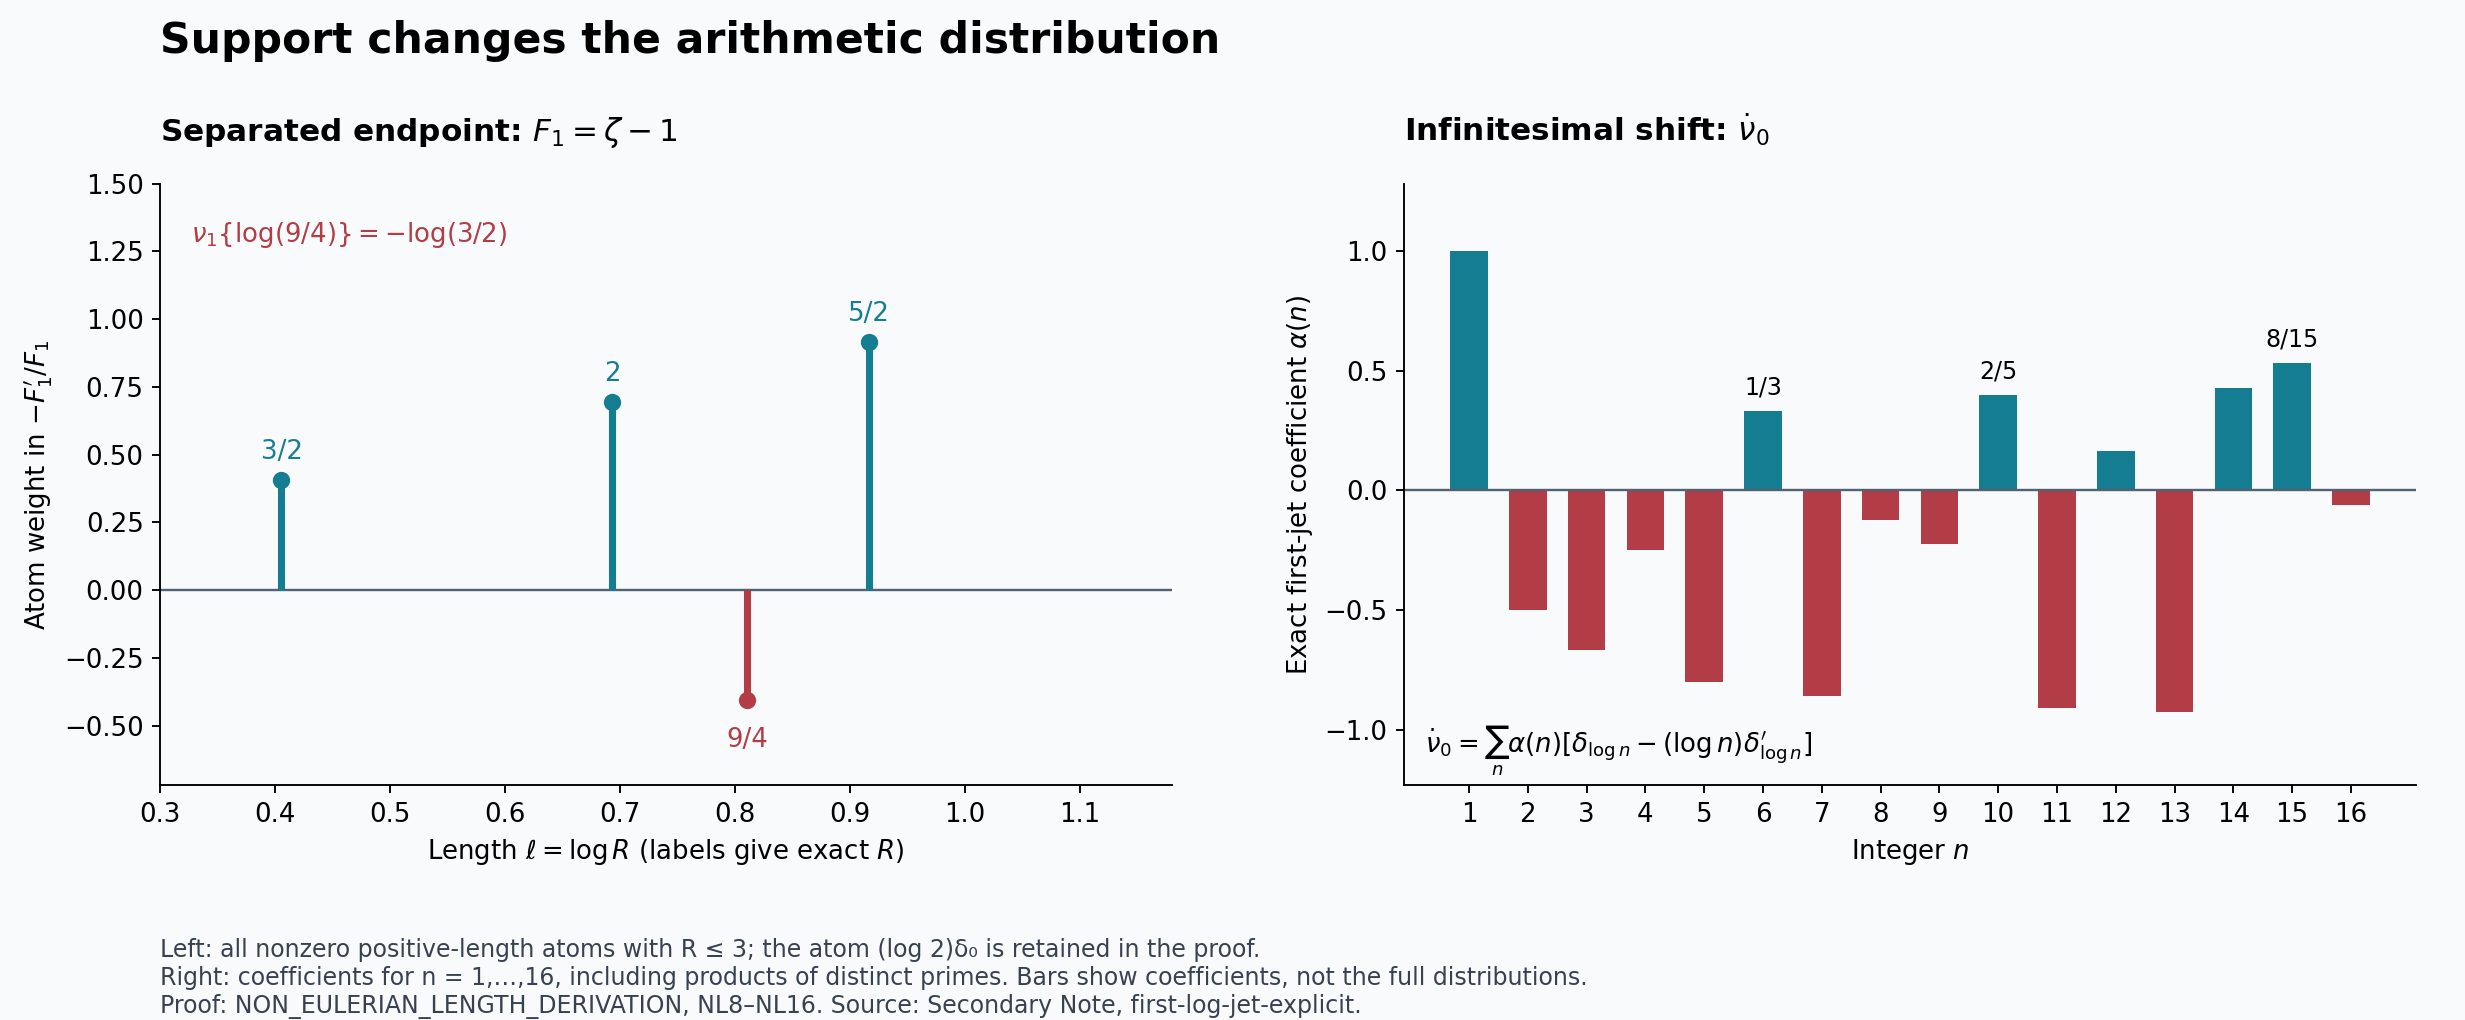
\includegraphics[keepaspectratio,alt={All nonzero positive-length atoms through ratio 3, and the exact first arithmetic coefficients; the zero-length mass is stated separately. Proof: NL7--NL16.}]{figures/24_non_eulerian_lengths.png}}
\caption{All nonzero positive-length atoms through ratio 3, and the
exact first arithmetic coefficients; the zero-length mass is stated
separately. Proof: NL7--NL16.}
\end{figure}

\clearpage

\section{The actual separated zeta sheet, its explicit formula, and its
positivity
defect}\label{the-actual-separated-zeta-sheet-its-explicit-formula-and-its-positivity-defect}

This calculation uses the quotient-size interpolation in the supplied
original LaTeX. It retains the supported arithmetic zero \(e\), the
unsupported element \(\tau\), the distinct residue quotients, the
completed-function endpoint residues, every gamma pole crossed by the
contour, and the functional-equation defect. The final countertest
concerns this particular shifted zeta sheet. It is not a counterexample
to the classical Riemann hypothesis.

Source coverage for this derivation:
\texttt{globalization\ nte/\allowbreak{}2/\allowbreak{}split\_\allowbreak{}zero\_\allowbreak{}secondary\_\allowbreak{}note.\allowbreak{}tex}, lines
1111--1555, read in full;
\texttt{globalization\ nte/\allowbreak{}4/\allowbreak{}split\_\allowbreak{}zero\_\allowbreak{}defect\_\allowbreak{}preprint\ (1).\allowbreak{}tex},
lines 500--854, read in full; the standing definitions, quotient sheets,
and shifted-deformation sections of
\texttt{globalization\ nte/\allowbreak{}5/\allowbreak{}some\ considerrations.\allowbreak{}tex} were read in the
returned source text. The whole-file read of the latter was truncated in
an unrelated middle section and is not recorded as complete. The
relevant named results are \texttt{thm:\allowbreak{}universal-\allowbreak{}taylor-\allowbreak{}deformation},
\texttt{cor:\allowbreak{}jets}, \texttt{thm:\allowbreak{}arithmetic-\allowbreak{}kernels-\allowbreak{}riemann},
\texttt{cor:\allowbreak{}first-\allowbreak{}log-\allowbreak{}jet-\allowbreak{}explicit},
\texttt{prop:\allowbreak{}hurwitz-\allowbreak{}standard-\allowbreak{}package}, and the defect preprint's
``Endpoint residues'' and ``Invariant/anti-invariant decomposition.''
The secondary note lists The Clankers;
\texttt{some\ considerrations.\allowbreak{}tex} lists ``The Clankers / prepared in
continuation''; the defect preprint has a blank author field. The
source-reading ledger maintained by the root task records canonical
source IDs. This file supplies the additional proofs below; it does not
claim those older formulas as new.

\subsection{SW1. The typed quotient maps and the interpolation they
actually
give}\label{sw1.-the-typed-quotient-maps-and-the-interpolation-they-actually-give}

Let \(S=G(\mathbb Z)=\mathbb Z\sqcup\{\tau\}\), with
\(e=0_{\mathbb Z}\ne\tau\). For \(n\ge1\), the two successive
surjections are \[
S\xrightarrow{\pi_n}G(\mathbb Z/n\mathbb Z)
\xrightarrow{p_n}\mathbb Z/n\mathbb Z,
\qquad
\pi_n(\tau)=\tau_n,\quad \pi_n(a)=a\bmod n,
\quad p_n(\tau_n)=0.
\tag{SW1}
\] The first target has \(n+1\) elements, and the second has \(n\).
Their zero fibres in the source are respectively \(\{\tau\}\) and
\(\{\tau\}\cup n\mathbb Z\). These statements follow directly from the
definitions, including at \(n=1\), when the first quotient has two
elements.

The two Dirichlet sums, and the supplied interpolation between their
numerical weights, are \[
F_t(s)=\sum_{n\ge1}(n+t)^{-s}=\zeta(s,1+t),\qquad
F_0=\zeta,\quad F_1=\zeta-1,
\quad 0\le t\le1.
\tag{SW2}
\] Initially these equalities hold for \(\Re s>1\). The identity at
\(t=1\) is a change of index in an absolutely convergent series. The
intermediate values are numerical interpolation of the cardinality
weights; they are not asserted to count a nonintegral number of elements
in a quotient.

In particular, SW2 is not the separate prime-weight Euler product
\(\prod_p(1-(p+1)^{-s})^{-1}\). Its distinction from that product is
proved with the actual quotient maps in TN1--TN9 of
\href{https://github.com/KokunoYumeto/zeta-function-research-reader/blob/173dbc6ed5a03235dbe7654f928f3692107db39b/workbenches/splitzero-tandem/branches/tau-zero-prime-positivity/TAU_WEIL_NORM_RECONSTRUCTION.md}{prime-norm
comparison proof}. For example the weights satisfy
\((m+1)(n+1)-(mn+1)=m+n\); retaining the labels gives the multiplicative
vector \((1,n)\), while summing its entries gives the nonmultiplicative
number \(n+1\).

\subsection{SW2. Analytic continuation and estimates used
below}\label{sw2.-analytic-continuation-and-estimates-used-below}

Write \(a=1+t\in[1,2]\). For any integer \(M\ge1\), Euler summation with
\(2M\) derivatives gives \[
\begin{aligned}
F_t(s)={}&\frac{a^{1-s}}{s-1}+\frac{a^{-s}}2
 +\sum_{j=1}^{M}\frac{B_{2j}}{(2j)!}(s)_{2j-1}a^{1-s-2j}\\
&-\frac{(s)_{2M}}{(2M)!}
\int_0^\infty \widetilde B_{2M}(x)(x+a)^{-s-2M}\,dx,
\qquad \Re s>1-2M.
\end{aligned}
\tag{SW3}
\] Here \(\widetilde B_k(x)=B_k(\{x\})\), and
\((s)_j=s(s+1)\cdots(s+j-1)\). To check the formula, apply integration
by parts on every interval \([n,n+1]\), using \(B_k'=kB_{k-1}\),
\(B_k(1)=B_k(0)\) for \(k\ne1\), and \(B_1(1)-B_1(0)=1\). Summing the
first boundary jumps gives the values \((n+a)^{-s}\). The remaining
boundaries at the lower end are the displayed half-value and even
Bernoulli terms; the upper boundaries tend to zero for \(\Re s>1\). The
derivative of order \(j\) of \((x+a)^{-s}\) is
\((-1)^j(s)_j(x+a)^{-s-j}\), giving the sign of the remainder. This
proves SW3 first for \(\Re s>1\). Since \(\widetilde B_{2M}\) is
bounded, its integral is absolutely and locally uniformly convergent for
\(\Re s>1-2M\), so it proves the asserted continuation there.

Letting \(M\) increase proves that \(F_t\) is meromorphic on
\(\mathbb C\) with its sole pole at 1, simple of residue 1. On each
fixed vertical strip, away from that pole, SW3 bounds \(F_t(s)\) by a
fixed polynomial in \(1+|\Im s|\), uniformly for \(t\in[0,1]\). Indeed
choose \(2M\) larger than one minus the left edge; the integral of
\((x+a)^{-\Re s-2M}\) is bounded uniformly on that strip, and
\((s)_{2M}\) is a polynomial. Derivatives in \(s\) satisfy the same kind
of bound by Cauchy's formula in a slightly larger strip. These
estimates, rather than a numerical approximation to a zero sum, justify
every infinite vertical integral below.

\subsection{SW3. The first infinitesimal is explicit and does not
vanish}\label{sw3.-the-first-infinitesimal-is-explicit-and-does-not-vanish}

Termwise differentiation, dominated uniformly on compact subsets of
\(\Re s>1\), gives \[
\partial_t F_t(s)=-sF_t(s+1),\qquad
\partial_t^jF_t(s)=(-1)^j(s)_j F_t(s+j).
\tag{SW4}
\] Analytic continuation gives these meromorphic identities everywhere.
In the dual-number ring \(\mathbb C[\epsilon]/(\epsilon^2)\), the
precise specialization is \[
F_\epsilon(s)=\zeta(s)-\epsilon s\zeta(s+1),\qquad
\log F_\epsilon=\log\zeta-\epsilon Q,
\quad Q(s)=s\frac{\zeta(s+1)}{\zeta(s)}.
\tag{SW5}
\] The logarithm equality is local on any open set where
\(\zeta\ne0,\infty\); its differentiated form is a global meromorphic
identity. In particular \[
\left.\partial_t\frac{F_t'}{F_t}\right|_{t=0}=-Q'(s),
\qquad
\left.\partial_t\left(-\frac{F_t'}{F_t}\right)\right|_{t=0}=Q'(s).
\tag{SW6}
\] The nilpotence \(\epsilon^2=0\) does not make the coefficient of
\(\epsilon\) zero: at \(s=2\), that coefficient in \(F_\epsilon\) is
\(-2\zeta(3)\ne0\).

For \(\Re s>1\), multiplying the absolutely convergent series of
\(1/\zeta(s)\) and \(\zeta(s+1)\) yields \[
Q(s)=s\sum_{n\ge1}\alpha(n)n^{-s},\quad
\alpha(1)=1,\qquad
\alpha(n)=(-1)^{\omega(n)}\frac{\prod_{p\mid n}(p-1)}n.
\tag{SW7}
\] The local factor is
\((1-p^{-s})/(1-p^{-s-1})=1-\sum_{k\ge1}(p-1)p^{-k}p^{-ks}\), which
proves the displayed coefficients. Their series is absolutely convergent
on \(\Re s>1\), also after one logarithmic differentiation. Thus \[
Q'(s)=\sum_{n\ge1}\alpha(n)(1-s\log n)n^{-s}.
\tag{SW8}
\] This first jet includes all squarefree-prime support combinations in
\(\alpha(n)\); it is not a single new prime-power term.

\subsection{SW4. Endpoint residues, logarithmic orders, and the full
reflection
defect}\label{sw4.-endpoint-residues-logarithmic-orders-and-the-full-reflection-defect}

Use exactly the supplied completion \[
\Lambda_t(s)=\pi^{-s/2}\Gamma(s/2)F_t(s),\qquad
\ell_t(s)=\Lambda_t'(s)/\Lambda_t(s).
\tag{SW9}
\] SW3 at zero, or the first Bernoulli polynomial, gives
\(F_t(0)=-1/2-t\). Hence \[
\operatorname {Res}_0\Lambda_t=-1-2t,\qquad
\operatorname {Res}_1\Lambda_t=1,
\quad
\operatorname {PP}_{0,1}\Lambda_t
=\frac{1+t}{s(s-1)}-t\frac{2s-1}{s(s-1)}.
\tag{SW10}
\] Both poles are simple for \(0\le t\le1\). Consequently \[
\operatorname {Res}_0\ell_t=\operatorname {Res}_1\ell_t=-1.
\tag{SW11}
\] For proof, a nonzero principal coefficient gives
\(\Lambda_t=(s-b)^{-1}u_t(s)\), with \(u_t(b)\ne0\); its logarithmic
derivative is \(-1/(s-b)+u_t'/u_t\). Thus the weight of the endpoint in
a logarithmic explicit formula is its order, not the coefficient
\(-1-2t\) of the original completed function.

At every negative even integer \(-2j\), \(j\ge1\), the precise order is
\[
\operatorname {ord}_{-2j}\Lambda_t
=\operatorname {ord}_{-2j}F_t-1.
\tag{SW12}
\] This formula also retains exceptional parameter values at which a
Hurwitz zero cancels a gamma pole. At \(t=1\), \(F_1(-2j)=-1\), so all
these completed poles are present and simple. In particular multiplying
only by \(s(s-1)\) does not make \(\Lambda_1\) entire.

Define the additive and logarithmic reflection defects by \[
\Delta_t(s)=\Lambda_t(s)-\Lambda_t(1-s),\qquad
d_t(s)=\ell_t(s)+\ell_t(1-s)
=\frac d{ds}\log\frac{\Lambda_t(s)}{\Lambda_t(1-s)}.
\tag{SW13}
\] These are explicit meromorphic objects. Their signs follow by the
chain rule. At \(t=0\), the classical functional equation gives both
defects zero. SW5--SW6 give the complete infinitesimal logarithmic
defect \[
\dot d_0(s)=-Q'(s)-Q'(1-s).
\tag{SW14}
\] Its endpoint residues vanish because \(Q\) is regular at both
endpoints: \(Q(0)=-2\), from \(s\zeta(s+1)\to1\), and \(Q(1)=0\). This
vanishing is only a statement about these two residues. It does not set
SW14 or the moving zero divisor to zero.

\subsection{SW5. Exact contour identity before invoking any
positivity}\label{sw5.-exact-contour-identity-before-invoking-any-positivity}

For entire functions \(f,g\), set \[
f^\#(s)=\overline{f(1-\bar s)},\qquad A(s)=f^\#(s)g(s),
\quad K(u)=A(1/2+iu),\quad
k(v)=\frac1{2\pi}\int_{\mathbb R}K(u)e^{iuv}\,du.
\tag{SW15}
\] In the formulas below the entire tests have Gaussian decay, up to a
polynomial factor, in each fixed vertical strip. We construct such tests
explicitly in SW9. The more general finite-rectangle residue identity
requires no decay hypothesis.

Fix \(c>1\) and let \(a_c=1-c\). First take a finite rectangle with
these two real edges and imaginary edges \(\pm T\), avoiding
nonremovable poles on its boundary. The residue theorem gives \[
\frac1{2\pi i}\oint\ell_t(s)A(s)\,ds
=\sum_{F_t(\rho)=0\ \mathrm{inside}}m_\rho A(\rho)
-A(1)-\sum_{j\ge0:\,-2j\ \mathrm{inside}}A(-2j).
\tag{SW16}
\] Zeros and gamma poles are written separately, so exact cancellations
in SW12 occur by addition of their integer orders. All quantities in
SW16 are finite.

If \(\ell_t A\), \(\ell_t(s)A(1-s)\), and \(\ell_t(1-s)A(1-s)\) have
only finitely many nonremovable poles in the strip and their horizontal
integrals tend to zero, then taking \(T\to\infty\) gives \[
\begin{aligned}
Z_{t,c}(A)-A(1)-\sum_{j\ge0:\,-2j>1-c}A(-2j)
={}&\frac1{2\pi i}\int_{\Re s=c}
\ell_t(s)(A(s)+A(1-s))\,ds\\
&-\frac1{2\pi i}\int_{\Re s=c}d_t(s)A(1-s)\,ds.
\end{aligned}
\tag{SW17}
\] Here \(Z_{t,c}(A)\) is the finite sum of the zero terms not
annihilated by \(A\), counted with multiplicity. The actual tests in SW9
satisfy every property in this sentence by a displayed cancellation
identity, so SW17 is used below without a missing analytic assumption.
For the sign, the left upward integral becomes the right upward integral
of \(\ell_t(1-s)A(1-s)\); the positive contour subtracts it.
Substituting \(\ell_t(1-s)=d_t(s)-\ell_t(s)\) proves SW17.

\subsection{SW6. The non-Eulerian arithmetic term and the completed
formula}\label{sw6.-the-non-eulerian-arithmetic-term-and-the-completed-formula}

Put \(a=1+t\), \(r_n=(n+t)/a\) for \(n\ge2\), and choose \(c\) so large
that \(\sum_{n\ge2}r_n^{-c}<1\). Write
\(r_{\boldsymbol n}=\prod_{i=1}^k r_{n_i}\). Absolute convergence of the
logarithm series gives \[
-\frac{F_t'}{F_t}(s)=\log a+
\sum_{k\ge1}\frac{(-1)^{k+1}}k
\sum_{n_1,\ldots,n_k\ge2}
\log r_{\boldsymbol n}\,r_{\boldsymbol n}^{-s}.
\tag{SW18}
\] To verify differentiation and absolute convergence, take a slightly
smaller real part on which the sum is still less than 1. Its positive
margin bounds the differentiated geometric series. Explicitly, if
\(B(c)=\sum r_n^{-c}<1\) and \(D(c)=\sum(\log r_n)r_n^{-c}<\infty\), the
sum of the absolute differentiated terms is
\(\sum_{k\ge1}D(c)B(c)^{k-1}=D(c)/(1-B(c))\). The general-length
derivation and its signed atoms are developed independently in
\href{https://github.com/KokunoYumeto/zeta-function-research-reader/blob/173dbc6ed5a03235dbe7654f928f3692107db39b/workbenches/splitzero-tandem/branches/tau-zero-prime-positivity/NON_EULERIAN_LENGTH_DERIVATION.md}{non-Eulerian
length proof}.

Define the absolutely convergent functional \[
\begin{aligned}
\mathcal L_t(k)={}&2\log(a)k(0)\\
&+\sum_{k_0\ge1}\frac{(-1)^{k_0+1}}{k_0}
\sum_{n_1,\ldots,n_{k_0}\ge2}
\frac{\log r_{\boldsymbol n}}{\sqrt{r_{\boldsymbol n}}}
\left[k(\log r_{\boldsymbol n})+k(-\log r_{\boldsymbol n})\right].
\end{aligned}
\tag{SW19}
\] Gaussian strip decay implies \(|k(v)|\le C_R e^{-R|v|}\) for every
fixed \(R>0\): shift the vertical contour defining \(k\) by \(R\) in the
appropriate direction. Choose \(R=c-1/2\), or a slightly larger value,
and the absolute majorant just proved for SW18 proves convergence of
SW19. All exchanges of its sum and integral are therefore justified.

Let \[
w_\infty(u)=\Re\psi(1/4+iu/2)-\log\pi,\qquad
\mathcal D_{t,c}(A)=\frac1{2\pi i}\int_{\Re s=c}d_t(s)A(1-s)\,ds.
\tag{SW20}
\] Then SW17 is exactly \[
\boxed{\begin{aligned}
Z_{t,c}(A)={}&A(1)+\sum_{j\ge0:\,-2j>1-c}A(-2j)\\
&+\frac1{2\pi}\int_{\mathbb R}K(u)w_\infty(u)\,du
-\mathcal L_t(k)-\mathcal D_{t,c}(A).
\end{aligned}}
\tag{SW21}
\] For completeness,
\(\ell_t=-\tfrac12\log\pi+\tfrac12\psi(s/2)+F_t'/F_t\). The gamma part
can be moved from \(c\) to \(1/2\) without crossing a gamma pole, and
reflection of the integration variable gives \(w_\infty\). The digamma
series on \(\Re(s/2)>0\) bounds it polynomially, so Gaussian decay kills
the horizontal edges. A term \(r^{-s}\) in SW18 integrates to
\(r^{-1/2}[k(-\log r)+k(\log r)]\), by shifting its entire integrand to
the critical line. The constant gives \(2\log(a)k(0)\). Finally the
minus sign of \(\mathcal D\) is the sign derived in SW17. This proves
every sign and endpoint contribution in SW21.

At \(t=0\), \(d_0=0\), and SW18 reduces to the usual logarithmic
prime-power series. For tests annihilating the classical trivial zeros,
\(A(-2j)=0\) for \(j\ge1\). SW21 then has exactly the two endpoints,
archimedean term, and prime term in WA24. At \(t=1\), neither the
negative-even terms nor \(\mathcal D_{1,c}\) can be dropped merely
because the original endpoint principal part has been computed.

\subsection{SW7. Local variation of the original zero
packet}\label{sw7.-local-variation-of-the-original-zero-packet}

Let \(\rho\) be an actual zero of \(\zeta\), of multiplicity \(m\), and
take a small circle containing no other zero and neither endpoint. Its
continuation as a zero cluster of \(F_t\) is counted by \[
T_t(A)=\frac1{2\pi i}\oint \frac{F_t'(s)}{F_t(s)}A(s)\,ds.
\tag{SW22}
\] The compact boundary is zero-free at \(t=0\), so uniform continuity
makes it zero-free for all sufficiently small \(t\). The argument
principle proves that this is the sum of \(A\) over the moving cluster,
counted with multiplicities. Differentiating on that compact contour and
integrating an exact derivative gives \[
\dot T_0(A)=-\frac1{2\pi i}\oint Q'(s)A(s)\,ds
=\operatorname {Res}_{s=\rho}\bigl(Q(s)A'(s)\bigr).
\tag{SW23}
\] The integration-by-parts equality follows from the zero contour
integral of \((QA)'\). It does not require the zero to be simple. If it
is simple, the result is \[
\dot\rho(0)=\frac{\rho\zeta(\rho+1)}{\zeta'(\rho)},\qquad
\dot T_0(A)=\dot\rho(0)A'(\rho).
\tag{SW24}
\] For a nontrivial zero, the numerator is nonzero because \(\rho\ne0\)
and \(\Re(\rho+1)>1\). Thus a simple nontrivial zero has a nonzero first
displacement in this interpolation. For a multiple zero, SW23 retains
the full residue of order up to \(m\), rather than assuming a
differentiable labeling of its individual branches.

The arithmetic first variation on the right-hand side is explicit as
well. With the conventions of SW15, the integral of
\(-Q'(s)(A(s)+A(1-s))\) on a right line is \[
\sum_{n\ge1}\frac{\alpha(n)}{\sqrt n}
\left[
\left(\frac{\log n}2-1\right)(k(-\log n)+k(\log n))
+\log n\,(k'(-\log n)-k'(\log n))
\right].
\tag{SW25}
\] To verify it, differentiation of the Fourier integral gives
\(\frac1{2\pi}\int(1/2+iu)K(u)e^{iuv}du=\tfrac12 k(v)+k'(v)\).
Reflection replaces the second derivative term by its negative. Insert
SW7 and differentiate termwise. Absolute convergence follows from the
same exponential contour bounds for \(k,k'\). The reflection correction
SW14 remains alongside SW25; omitting it is not a deformation of the
same contour identity.

\subsection{SW8. The exact symmetric lift and the missing Hermitian
property}\label{sw8.-the-exact-symmetric-lift-and-the-missing-hermitian-property}

Let \[
G_t(s)=(s-1)F_t(s),\qquad
H_t(s)=G_t(s)G_t(1-s)=-s(s-1)F_t(s)F_t(1-s).
\tag{SW26}
\] Both \(G_t\) and \(H_t\) are entire by SW3. They have real
conjugation symmetry, and \(H_t(1-s)=H_t(s)\). The actual map is the
multiplicative norm for the involution on entire functions, \[
N:\mathcal O(\mathbb C)\longrightarrow\mathcal O(\mathbb C)^{s\mapsto1-s},
\qquad N(G)(s)=G(s)G(1-s).
\tag{SW27}
\] It satisfies \(N(G_1G_2)=N(G_1)N(G_2)\), and its divisor is the
original divisor plus its reflected divisor, with multiplicities. It is
not asserted to be additive or to preserve the zero count without
doubling. On the critical line \(H_t(s)=|G_t(s)|^2\ge0\).

The zero pairing of \(H_t\), on finite packets closed under
\(\rho\mapsto1-\bar\rho\), is Hermitian. Proof: applying complex
conjugation and this permutation to
\(\sum m_\rho\overline{f(1-\bar\rho)}g(\rho)\) exchanges \(f\) and
\(g\). By contrast, a divisor lacking that permutation symmetry need not
define a Hermitian form. The next calculation proves the failure, and a
negative direction in the symmetric lift, for the specific endpoint
\(t=1\).

\subsection{SW9. A fully explicit negative test for the separated
endpoint}\label{sw9.-a-fully-explicit-negative-test-for-the-separated-endpoint}

The exact special values are \[
F_1(-20)=-1,\qquad
F_1(-19)=\frac{174611}{6600}-1=\frac{168011}{6600}>0.
\tag{SW28}
\] They follow from \(\zeta(-n)=-B_{n+1}/(n+1)\), \(B_{21}=0\), and
\(B_{20}=-174611/330\), also obtainable from SW3. Continuity therefore
gives at least one real zero in \((-20,-19)\). Define \(\alpha\) to be
the least such real zero. This is well-defined: the endpoint values
exclude neighborhoods of the two endpoints, and a nonzero holomorphic
function has only finitely many zeros in the remaining compact interval.
Write \(m\ge1\) for its exact multiplicity, and put
\(\beta=1-\alpha\in(20,21)\).

Since \(F_1(\sigma)=\sum_{n\ge2}n^{-\sigma}>0\) for real \(\sigma>1\),
\(\beta\) is not a zero of \(F_1\). The divisor of \(H_1\), however, has
both \(\alpha\) and \(\beta\), each with multiplicity \(m\). Define \[
h(s)=(s-\alpha)^m(s-\beta)^m,\qquad
W(s)=e^{(s-1/2)^2}\frac{H_1(s)}{h(s)}.
\tag{SW29}
\] The quotient is entire, \(W(\alpha),W(\beta)\ne0\), and \(W^\#=W\).
Indeed reflection exchanges the two factors of \(h\) with total sign
\((-1)^{2m}=1\), and all the coefficients are real. SW3 proves that
\(W\) and every fixed derivative are bounded by a polynomial times
\(e^{-(\Im s)^2}\) on each fixed vertical strip; away from a bounded
region the denominator is a polynomial bounded below by a positive
constant times \(|\Im s|^{2m}\), and inside that region removability
gives boundedness.

For arbitrary prescribed \(z_\alpha,z_\beta\in\mathbb C\), take the
degree-at-most-one polynomial \[
q(s)=\frac{z_\alpha}{W(\alpha)}\frac{s-\beta}{\alpha-\beta}
+\frac{z_\beta}{W(\beta)}\frac{s-\alpha}{\beta-\alpha},
\qquad f=qW,\quad A=f^\#f.
\tag{SW30}
\] Then \(f(\alpha)=z_\alpha\) and \(f(\beta)=z_\beta\). At every other
zero of \(H_1\), \(W\) vanishes at least to the full multiplicity.
Therefore \(A\) annihilates all of those zero terms. Take the strip
\(-21<\Re s<22\). Its native and symmetric zero functionals are exactly
\[
Z_{1,22}(A)=m\overline{z_\beta}z_\alpha,
\qquad
Z_{H_1}(A)=m(\overline{z_\beta}z_\alpha+\overline{z_\alpha}z_\beta).
\tag{SW31}
\] No other zero contributes, including a multiple zero or a zero with
large imaginary part, because of the preceding vanishing orders.

For \((z_\alpha,z_\beta)=(1,-1)\), this gives \[
\boxed{Z_{1,22}(f^\#f)=-m<0,\qquad Z_{H_1}(f^\#f)=-2m<0.}
\tag{SW32}
\] For \((z_\alpha,z_\beta)=(1,i)\), it gives \[
\boxed{Z_{1,22}(f^\#f)=-im,}
\tag{SW33}
\] which is not real. Thus the original shifted divisor pairing is not
Hermitian, and the exact symmetric lift has a genuine negative
direction. Nonnegativity of \(H_1\) as a function on the critical line,
proved in SW8, does not imply nonnegativity of its zero pairing.

Here are the promised contour checks for the actual tests. Since \[
\frac{H_1'}{H_1}A
=q^\#q\,e^{2(s-1/2)^2}\frac{H_1'H_1}{h^2},
\tag{SW34}
\] the only possible nonremovable poles are at \(\alpha,\beta\). Every
other zero is canceled as an identity of meromorphic functions. SW3 and
its differentiated estimate bound the numerator polynomially on each
strip, so the horizontal edges tend to zero with Gaussian speed.
Likewise, using \(H_1=G_1G_1(1-s)\), each occurrence of \(F_1'/F_1\) or
its reflected counterpart multiplied by \(A\) cancels a factor of
\(F_1\) in \(H_1^2\). The same assertion holds for \(A(1-s)\), since its
denominator is the same reflection-invariant \(h^2\). The remaining
digamma factors have finitely many poles in this strip and at most
polynomial growth on high horizontal edges, by the digamma recurrence
and its convergent right-half-plane series. Consequently SW17--SW21
apply with no unproved horizontal zero-avoidance estimate.

At \(t=1,c=22\), the absolute logarithm expansion required in SW18
holds. For instance \[
\sum_{n\ge2}\left(\frac2{n+1}\right)^{22}
\le\left(\frac23\right)^{22}
+\int_3^\infty\left(\frac2x\right)^{22}dx
=\left(\frac23\right)^{22}\left(1+\frac3{21}\right)<1.
\tag{SW35}
\] Thus the corrected explicit formula evaluated on the negative test is
the exact equality \[
\boxed{
-m=A(1)+\sum_{j=0}^{10}A(-2j)
+\frac1{2\pi}\int_{\mathbb R}|f(1/2+iu)|^2w_\infty(u)du
-\mathcal L_1(k)-\mathcal D_{1,22}(A).
}
\tag{SW36}
\] Every term is defined in SW15 and SW19--SW20, and every series and
integral converges by the estimates above. This is a concrete positivity
analysis of the actual non-Eulerian separated sheet, including its
retained completion and reflection terms. It does not insert an
arbitrary Euler factor for the supported-zero prime.

The tested divisor is the full shifted divisor in the strip
\(-21<\Re s<22\), and its selected real zero lies outside the classical
critical strip. Thus SW32 does not establish nonpositivity for a
separately defined pairing restricted to \(0<\Re s<1\). Nor does it rule
out a different boundary subtraction or a selected positivity cone. Such
an operation must specify its map and retain the component it removes.
The exact maps for this detected component are given next.

\subsection{SW10. The retained two-point object and its positive and
negative
projections}\label{sw10.-the-retained-two-point-object-and-its-positive-and-negative-projections}

Keep the actual function \(W\) of SW29 and define the vector space \[
V=W\mathbb C[s],\qquad
E:V\longrightarrow\mathbb C^2,\quad E(f)=(f(\alpha),f(\beta)).
\tag{SW37}
\] Let \(j:\mathbb C^2\to V\) be the interpolation formula SW30. Direct
evaluation proves \(Ej=\operatorname{id}\). Since
\(W(\alpha),W(\beta)\ne0\), a polynomial multiple \(qW\) lies in
\(\ker E\) precisely when \(q\) is divisible by both distinct linear
factors. Hence \[
K:=\ker E=W(s-\alpha)(s-\beta)\mathbb C[s],\qquad
V=j(\mathbb C^2)\oplus K.
\tag{SW38}
\] The decomposition is explicit: \(f=jE(f)+(f-jE(f))\), and its second
term lies in \(K\). An element of the intersection has evaluation both
equal to its coefficient vector and zero, proving directness.

For \(z=E(f)\) and \(w=E(g)\), the native and reflected pairings factor
through these maps as \[
B_{\mathrm{nat}}(f,g)=m\overline{z_\beta}w_\alpha,\qquad
B_{\mathrm{sym}}(f,g)=m(\overline{z_\beta}w_\alpha+\overline{z_\alpha}w_\beta).
\tag{SW39}
\] The same cancellation used in SW31 proves this for arbitrary
\(f,g\in V\). Both forms vanish when either input lies in \(K\). The
descended matrix of \(B_{\mathrm{sym}}\) is
\(m\left(\begin{smallmatrix}0&1\\1&0\end{smallmatrix}\right)\), which is
invertible, so its full radical is exactly \(K\). Also
\(B_{\mathrm{sym}}=B_{\mathrm{nat}}+B_{\mathrm{nat}}^{*}\), where
\(B^*(f,g)=\overline{B(g,f)}\); this is the exact passage to the
Hermitian part, including its factor of two.

Define \[
\Pi_+=\frac12\begin{pmatrix}1&1\\1&1\end{pmatrix},\qquad
\Pi_-=\frac12\begin{pmatrix}1&-1\\-1&1\end{pmatrix},\qquad
P_\pm=j\Pi_\pm E,\quad P_K=1-jE.
\tag{SW40}
\] Multiplication gives \(\Pi_\pm^2=\Pi_\pm\), \(\Pi_+\Pi_-=0\), and
\(\Pi_++\Pi_-=1\). Using \(Ej=1\) proves that \(P_+,P_-,P_K\) are
mutually annihilating idempotents summing to \(1_V\). Their images are
respectively \(j\mathbb C(1,1)\), \(j\mathbb C(1,-1)\), and \(K\). These
three summands are orthogonal for \(B_{\mathrm{sym}}\). To verify all
signs and the orthogonality, write \[
c_+(f)=\frac{f(\alpha)+f(\beta)}2,\qquad
c_-(f)=\frac{f(\alpha)-f(\beta)}2.
\] Substitution in SW39 gives \[
B_{\mathrm{sym}}(f,g)=2m\overline{c_+(f)}c_+(g)
-2m\overline{c_-(f)}c_-(g).
\tag{SW41}
\] Thus the nonnegative cone is exactly \(\{|c_-|\le|c_+|\}\), with the
radical directions retained, and \(j\mathbb C(1,1)\oplus K\) is a
maximal nonnegative linear subspace. Indeed any vector outside it has
\(c_-\ne0\); subtracting its positive component, already in this
subspace, gives a negative vector by SW41, so it cannot be adjoined
while preserving nonnegativity.

A particular boundary subtraction can now be defined, rather than left
implicit: \[
B_+(f,g):=B_{\mathrm{sym}}(f,g)+2m\overline{c_-(f)}c_-(g)
=B_{\mathrm{sym}}(P_+f,P_+g)=2m\overline{c_+(f)}c_+(g).
\tag{SW42}
\] It is positive semidefinite, and its removed negative direction is
exactly the recorded image of \(P_-\). Equations SW37--SW42 identify the
defect object, its quotient, section, radical, orthogonal summands, and
one exact corrected form. They do not claim that this particular
subtraction is the arithmetic or prismatic choice required elsewhere in
the programme; they provide the complete finite object such a comparison
would have to map.

\subsection{SW11. Consequences for the programme's
vanishing-infinitesimal
question}\label{sw11.-consequences-for-the-programmes-vanishing-infinitesimal-question}

The exact distinctions now have proved maps. The quotient-size
construction SW1 maps to the interpolation SW2; its first-order base
change is SW5; its completed divisor is measured by SW16; its failure of
reflection is the meromorphic function SW13; and its reflected Hermitian
lift is the norm map SW27. The first-order endpoint residue variation of
the logarithmic derivative is zero, while the first-order function,
logarithmic derivative, and moving zero cluster are respectively SW5,
SW6, and SW23 and need not vanish. SW24 proves nonvanishing of the
displacement at every simple nontrivial classical zero.

The previously derived prime-weight formula TN21 concerns a different
function, a holomorphic-unit multiple of classical \(\zeta\) in
\(\Re s>0\). Its unchanged zero divisor and corrected archimedean term
cannot be transferred to \(F_1=\zeta-1\). The actual map from this
interpolation to a symmetric divisor is SW27, which adds the reflected
divisor and exposes SW32. A prismatic or deformation comparison must
carry these explicit objects and the reflection defect through its maps;
nilpotence of a parameter or vanishing of an endpoint residue does not
erase them.

\clearpage

\section{Reconstruction over the full support
lattice}\label{reconstruction-over-the-full-support-lattice}

This calculation starts from the programme's actual support-amplitude
semiring. It proves the precise comparison with the earlier scalar
calculations, identifies information lost by all separate Boolean branch
maps after linearization, and constructs a support-valued extension of
the finite Weil packet form. It does not assert that a zeta zero off the
critical line exists, or that positivity for the classical Weil
distribution has been proved.

The source definition and the existing spectrum theorem are in
\emph{Split Support Geometry: Universal Zero Fibres, Arithmetic Curves,
and Frobenius-Perfect Quantization}, The Clankers, June 2026, Version
11. The file read for this derivation is
\texttt{split\_\allowbreak{}support\_\allowbreak{}geometry\_\allowbreak{}arithmetic\_\allowbreak{}curve\_\allowbreak{}v11910.\allowbreak{}tex}, SHA256
\texttt{8443cc04\allowbreak{}01b18d37\allowbreak{}3939d992\allowbreak{}f0a2f538\allowbreak{}4ee2fa11\allowbreak{}30f05975\allowbreak{}3d5f3972\allowbreak{}eec5052d},
Definition \texttt{def:\allowbreak{}lattice-\allowbreak{}split}, Theorems
\texttt{thm:\allowbreak{}lattice-\allowbreak{}normal-\allowbreak{}form},
\texttt{thm:\allowbreak{}birkhoff-\allowbreak{}support-\allowbreak{}coordinates},
\texttt{thm:\allowbreak{}lattice-\allowbreak{}prime-\allowbreak{}classification},
\texttt{thm:\allowbreak{}spectral-\allowbreak{}ordinal-\allowbreak{}sum}, and \texttt{thm:\allowbreak{}support-\allowbreak{}base-\allowbreak{}change},
source lines1180--1871. Those results are prior programme mathematics.
The different file
\texttt{split\_\allowbreak{}support\_\allowbreak{}geometry\_\allowbreak{}arithmetic\_\allowbreak{}curve\_\allowbreak{}v11.\allowbreak{}tex}, SHA256
\texttt{5fa6a55a\allowbreak{}a9d1a2e5\allowbreak{}7599e206\allowbreak{}087d3d24\allowbreak{}66b25dd9\allowbreak{}9fa1a90d\allowbreak{}5f86367a\allowbreak{}afab1b4d},
has the explicit branch-spectrum theorem at lines1925--1985. The
editions are not treated as byte-identical.

\subsection{1. The base and its split comparison
maps}\label{the-base-and-its-split-comparison-maps}

Let R be a nonzero commutative unital ring and L a nontrivial bounded
distributive lattice. Write its bounds as 0\_L and 1\_L. Set \[
S_L=G_L(R)=\{z_\lambda=(0,\lambda):\lambda\in L\}
\cup\{\widehat r=(r,1_L):r\in R\},
\quad z_{1_L}=\widehat0=e_L,\quad z_{0_L}=\tau_L.
\tag{FSR1}
\] The overlap in this union consists of the one element e\_L. The
operations are \[
(r,\lambda)+(s,\mu)=(r+s,\lambda\vee\mu),\qquad
(r,\lambda)(s,\mu)=(rs,\lambda\wedge\mu).
\tag{FSR2}
\] In particular, \(\widehat r+z_\lambda=\widehat r\) and
\(\widehat r z_\lambda=z_\lambda\), including r=0. Closure follows
because every nonzero amplitude has top support. The semiring laws
follow from those of R and the distributive lattice law. Its zero is
tau\_L and its unit is widehat1.

Put S=G\_B(R), with B=\{0,1\}. The endpoint inclusion and each Boolean
branch give maps \[
\iota:S\longrightarrow S_L,\quad \tau\mapsto\tau_L,\quad r\mapsto\widehat r,
\qquad
\beta_\epsilon:S_L\longrightarrow S,\quad
z_\lambda\mapsto z_{\epsilon(\lambda)},\quad \widehat r\mapsto r,
\qquad \beta_\epsilon\iota=\mathrm{id}_S.
\tag{FSR3}
\] Here epsilon:L→B preserves the bounds, joins, and meets. Both maps
preserve every operation in FSR2: on the zero fibre this is the
lattice-map identity; on two supported amplitudes it is the identity of
R; on a mixed pair it follows from the two identities after FSR2. Thus
iota is injective and every beta\_epsilon is surjective. The kernel
congruence of beta\_epsilon identifies exactly the zero-fibre elements
with the same epsilon value, and no two distinct nonzero amplitudes. Its
inverse image of the actual scalar zero is \[
\beta_\epsilon^{-1}(\tau)=\{z_\lambda:\epsilon(\lambda)=0\}.
\tag{FSR4}
\] Its inverse image of the supported scalar zero is the complementary
set of zero-fibre elements. This is the exact distinction between a zero
ideal and a congruence in this comparison.

The amplitude projection p\_L:S\_L→R has zero fibre Z\_L=\{z\_lambda\}.
Every homomorphism to a ring kills Z\_L: the equality
e\_L+z\_lambda=e\_L implies this by additive cancellation in the target.
The restriction to the supported copy then gives a unique ring
homomorphism R→A. This proves the universal property of p\_L, without
identifying e\_L with tau\_L in S\_L.

For a domain R, the supported zero is a prime element in the
divisibility sense: \[
e_L S_L=Z_L,
\qquad e_L\mid xy\ \Longleftrightarrow\ p_L(x)p_L(y)=0
\ \Longleftrightarrow\ e_L\mid x\ \text{or}\ e_L\mid y.
\tag{FSR5}
\] The first equality follows from e\_L z\_lambda=z\_lambda and e\_L
widehat r=e\_L. The next equivalence follows from the first equality and
the multiplication law. The last uses precisely the absence of zero
divisors in R. The ideal Z\_L is proper because widehat1 is outside it.
The element e\_L is not a unit, since every product with it has
amplitude zero. It is reducible, since e\_L=e\_L e\_L with two nonunits.
Its primality and its multiplicative idempotence are simultaneous facts.

For completeness the entire semiring-prime comparison can be obtained
directly. If an ideal contains a supported amplitude, multiplication by
e\_L puts e\_L in it, hence puts all of Z\_L in it. Its supported
amplitudes form a ring ideal J. An ideal containing no supported
amplitude is Z\_a for a proper lattice ideal a: joins follow from
addition and downward closure follows from z\_mu z\_lambda=z\_mu when
mu≤lambda. Thus all ideals are Z\_a and \[
Q_J=Z_L\cup\{\widehat r:r\in J\}.
\tag{FSR6}
\] Testing FSR2 shows that Z\_a is prime exactly when a is a prime
lattice ideal, and Q\_J is prime exactly when J is a ring prime. Every
support prime is strictly below every arithmetic prime. For R=Z this
includes \[
Z_{\mathfrak a}\subsetneq Z_L=(e_L)=Q_{(0)}\subsetneq Q_{(p)}.
\tag{FSR7}
\] The basic opens are D(z\_lambda)=\{Z\_a:lambda∉a\} and D(widehat
r)=Spec\_lat(L) union D\_R(r). These formulas prove the topological
ordinal sum, including its topology. Contraction along beta\_epsilon
sends the scalar prime \{tau\} to Z\_(epsilon inverse0) and Q\_q to
Q\_q. Contraction along iota sends every Z\_a to \{tau\} and Q\_q to
Q\_q. Consequently the scalar spectrum is a retract with an explicitly
chosen section; it is not the entire support spectrum.

\subsection{2. Joint reconstruction before
linearization}\label{joint-reconstruction-before-linearization}

Now assume L finite and let J(L) be its nonzero join-irreducible
elements. For j∈J(L) put theta\_j(lambda)=1 if j≤lambda and 0 otherwise.
A join-irreducible is join-prime: if j≤lambda∨mu, distributivity gives
j=(j∧lambda)∨(j∧mu), so one term equals j. Therefore theta\_j is a
bounded lattice homomorphism. Every nonzero element is the join of the
join-irreducibles below it, by induction in the finite partially ordered
set. Hence these characters jointly distinguish elements of L.

Conversely, a Boolean branch has a prime filter whose least element j is
the meet of its elements. If j=x∨y with neither x nor y equal to j, the
primality of the filter contradicts the minimality of j. Thus j is
join-irreducible, and the branch is theta\_j. This proves the entire
branch list.

The product of all branch maps is the injective semiring map \[
\Beta:S_L\longrightarrow\prod_{j\in J(L)}S,\qquad
\Beta(x)=(\beta_j(x))_j.
\tag{FSR8}
\] Its image is exactly the following set. All coordinate amplitudes
have a common value r. If r≠0, all coordinates are the same supported
element r. If r=0, each coordinate is tau or e, and the set of
coordinates equal to e is an order ideal in J(L). Indeed it is
\{j:j≤lambda\} for the source z\_lambda. Conversely, an order ideal A
gives lambda=join A; join-primality shows that \{j:j≤lambda\}=A. This
proves both surjectivity onto the displayed image and injectivity.

For L=B\^{}d the poset J(L) is an antichain of d atoms. Every subset is
an order ideal, so FSR8 becomes an isomorphism \[
G_{B^d}(R)\ \cong\ \underbrace{G(R)\times_R\cdots\times_R G(R)}_{d\text{ factors}},
\tag{FSR9}
\] where the maps to R are amplitude projections. This is different from
the product of independent amplitude coordinates: the common-amplitude
condition is part of the isomorphism, not an omitted restriction.

For a general finite distributive L, FSR8 is the subsemiring of that
fibre product whose zero-amplitude masks satisfy the stated order-ideal
relations. The additive and multiplicative laws remain FSR2. All earlier
scalar identities pull back along each beta\_j. Conversely, if two
S\_L-valued expressions have equal images under every beta\_j, FSR8
proves equality in S\_L. This last conclusion concerns semiring-valued
expressions; it does not yet concern their free additive envelopes.

\subsection{3. The exact extra kernel created by
linearization}\label{the-exact-extra-kernel-created-by-linearization}

For a commutative coefficient ring k define the contracted meet algebra
\[
C_L=k[(L,\wedge)]/([0_L]).
\tag{FSR10}
\] It is free as a k-module on u\_lambda={[}lambda{]} for lambda≠0\_L,
with u\_0=0, unit u\_1, and u\_lambda u\_mu=u\_(lambda∧mu). It retains
multiplication from support and introduces its own additive linear
combinations. In particular u\_(lambda∨mu) is not defined to be
u\_lambda+u\_mu.

For every nonzero a∈L, whether join-irreducible or not, define \[
\eta_a(u_\lambda)=\mathbf1_{\{a\leq\lambda\}}.
\tag{FSR11}
\] This is a unital k-algebra homomorphism: a≤lambda∧mu holds exactly
when both inequalities hold. With any linear extension of the order, its
matrix has entries 1\_(a≤lambda), is triangular with diagonal1, and is
invertible over the integers. Consequently \[
\eta:C_L\xrightarrow{\sim}\prod_{a\in L\setminus\{0\}}k.
\tag{FSR12}
\] No division in k is used.

An explicit inverse uses the Möbius function of the finite order. Define
mu(a,a)=1 and, for a\textless b, mu(a,b)=-sum\_(a≤c\textless b)mu(a,c).
The upper triangular incidence matrix Z\_(ab)=1\_(a≤b) has inverse with
these entries: the recurrence proves MZ=I, and finite triangular
matrices then also satisfy ZM=I. Define \[
E_a=\sum_{\lambda\leq a}\mu(\lambda,a)u_\lambda.
\tag{FSR13}
\] Then eta\_b(E\_a)=sum\_(b≤lambda≤a)mu(lambda,a)=delta\_(ab). The term
lambda=0 contributes zero. Thus \[
E_aE_b=\delta_{ab}E_a,\qquad
\sum_{a\neq0}E_a=u_1,\qquad
u_\lambda=\sum_{0<a\leq\lambda}E_a.
\tag{FSR14}
\] These identities follow by applying the isomorphism FSR12, so hold
over every coefficient ring.

The linearized Boolean branch theta\_j is precisely eta\_j. Write \[
K_L=\bigcap_{j\in J(L)}\ker\eta_j
=\bigoplus_{a\in L\setminus(\{0\}\cup J(L))}kE_a.
\tag{FSR15}
\] This proves the full kernel, not only its dimension. Over a field its
dimension is \textbar L\textbar−1−\textbar J(L)\textbar. It is a direct
product of copies of k, with multiplicatively idempotent coordinate
projectors. It is zero exactly when every nonzero lattice element is
join-irreducible, equivalently when L is a chain. To verify the last
equivalence, a chain has that property. If L is not a chain, choose
incomparable a,b; then a∨b is nonzero and join-reducible.

For L=B\^{}2=\{0,a,b,1\}, with a∧b=0 and a∨b=1, \[
E_a=u_a,\qquad E_b=u_b,\qquad
w=E_1=u_1-u_a-u_b,
\quad w^2=w\neq0,
\quad\eta_a(w)=\eta_b(w)=0.
\tag{FSR16}
\] Indeed the three terms are distinct basis vectors, proving nonzero,
and direct expansion gives
\((u_1-u_a-u_b)^2=u_1+u_a+u_b-2u_a-2u_b=u_1-u_a-u_b\). Thus the semiring
branch maps in FSR8 distinguish every support element, but their
separately linearized maps omit w. This is a proved failure of
linearized reconstruction from separate branches. Its retained object is
K\_L with inclusion, coordinate projectors, and quotient given in FSR15.

The nonzero a that are not join-irreducible give genuine mixed
observables. For a with join-irreducible decomposition a=join\_(j≤a)j,
\[
\eta_a(u_\lambda)=\prod_{j\leq a}\theta_j(\lambda).
\tag{FSR17}
\] Both sides are1 exactly when every j≤a lies below lambda,
equivalently when a≤lambda. Thus a joint product of branch tests
restores this missing coordinate. Separate branch expectations do not
determine expectations of these products. FSR12 gives the complete
recovery map using all these joint tests.

\subsection{4. Contracted multiplicative coefficients and the scalar
retract}\label{contracted-multiplicative-coefficients-and-the-scalar-retract}

Let Gamma\_L=k{[}(S\_L, multiplication){]}/({[}tau\_L{]}). Put
E={[}e\_L{]} and F=1−E. Multiplication by E sends {[}z\_lambda{]} to
itself and {[}widehat r{]} to {[}e\_L{]}. Thus E Gamma\_L is C\_L,
embedded by u\_lambda↦{[}z\_lambda{]}. The complementary factor F
Gamma\_L has basis \[
v_r=[\widehat r]-[e_L],\qquad r\in R\setminus\{0\},
\tag{FSR18}
\] and v\_0=0. Their multiplication is v\_r v\_s=v\_(rs), with zero when
rs=0. Indeed expansion gives
{[}widehat(rs){]}−{[}e\_L{]}−{[}e\_L{]}+{[}e\_L{]}. The two sets
\{{[}z\_lambda{]}:lambda≠0\} and \{v\_r:r≠0\} form a basis: each
original nonzero supported basis element is v\_r+{[}e\_L{]}, and
comparison of the distinct {[}widehat r{]} coefficients proves linear
independence. Hence \[
\Gamma_L\cong C_L\times D_R,
\qquad D_R=k[(R,\times)]/([0_R]).
\tag{FSR19}
\] The formulas prove this for rings with zero divisors as well as
domains. For R=Z the second factor is \[
D_{\mathbb Z}\cong k[t,X_p:p\text{ rational prime}]/(t^2-1),
\quad v_{-1}\mapsto t,\quad v_p\mapsto X_p.
\tag{FSR20}
\] Unique prime factorization of every nonzero integer proves a
bijection of the displayed monomial bases and compatibility with
multiplication.

For scalar support the same construction is Gamma\_B=k×D\_R. Under FSR19
each branch and the scalar inclusion become \[
\Gamma(\beta_j):(c,d)\longmapsto(\eta_j(c),d),
\qquad
\Gamma(\iota):(a,d)\longmapsto(a\,u_1,d).
\tag{FSR21}
\] These formulas follow on z\_lambda and widehat r, which generate the
algebras. The composite is the identity. The intersection of all branch
kernels is exactly K\_L×0. Thus the earlier arithmetic prime-label
algebra D\_R is preserved as an actual direct factor, and the missing
support coefficient object is explicitly identified. This is stronger
than saying that earlier work might survive.

The evaluation map Gamma\_L→R when k=Z sends {[}widehat r{]} to r and
every {[}z\_lambda{]} to0. For R=Z, FSR19--20 identify its kernel as \[
C_L\times (t+1,\ X_p-p\text{ for every prime }p)\subset C_L\times D_{\mathbb Z}.
\tag{FSR22}
\] The quotient of D\_Z by the displayed ideal is Z: every polynomial
reduces to its integer evaluation, and that evaluation is the inverse of
the resulting inclusion of Z. This proves equality of the kernel ideal.
In particular all of C\_L, including K\_L, is killed by arithmetic
addition. It remains present before that quotient. The inclusion and
quotient in FSR19 and FSR22 give its exact relation to the arithmetic
factor.

\subsection{5. Extension of complexes, operators, and all primary
jets}\label{extension-of-complexes-operators-and-all-primary-jets}

Take k=C for this section. Let (V\^{}bullet,d) be any specified complex
of complex vector spaces, with its original differentials. Its full
support extension is \[
V_L^\bullet=C_L\otimes_{\mathbb C}V^\bullet
=\bigoplus_{a\neq0}E_a\otimes V^\bullet,
\qquad d_L(E_a\otimes v)=E_a\otimes dv.
\tag{FSR23}
\] This is a defined construction, not an identification with a
prismatic complex. Decomposition FSR14 proves directly \[
\ker d_L=\bigoplus_a E_a\otimes\ker d,
\qquad\operatorname{im}d_L=\bigoplus_a E_a\otimes\operatorname{im}d,
\qquad H^q(V_L)=\bigoplus_a E_a\otimes H^q(V).
\tag{FSR24}
\] The first two equalities follow by equating the coefficients of the
independent E\_a. The third is their quotient. Thus a nonzero cohomology
class of a specified old complex remains nonzero in every individual
support sector. For every linear chain map T, the map 1⊗T preserves all
sectors. A homotopy dH+Hd=T−T' extends to 1⊗H and satisfies the
identical formula. The maps eta\_j⊗id are chain maps, with joint kernel
K\_L⊗V\^{}bullet. The scalar inclusion v↦u\_1⊗v is split by every
eta\_j⊗id. These formulas specify exactly which part of this statement
is functorial and which prismatic comparison still requires identifying
the actual input complex.

For the finite packet take the four distinct points \[
\alpha_1=\rho,\qquad\alpha_2=1-\overline\rho,\qquad
\alpha_3=\overline\rho,\qquad\alpha_4=1-\rho,
\] where \(\rho=1/2+\delta+i\gamma\), \(0<\delta<1/2\) and \(\gamma>2\).
Put \(d(s)=\prod_{i=1}^4(s-\alpha_i)\), \(h=d^m\) with \(m\ge1\), and
\(A_h=\mathbb C[s]/(h)\). These parameters define a finite algebra for
every such \(\rho\); they do not assert that \(\rho\) is a zeta zero.
Pairwise coprimality gives the isomorphism to the four rings
\(\mathbb C[t_i]/(t_i^m)\) by Taylor coefficients. To see its inverse
explicitly, take \(h_i=h/(s-\alpha_i)^m\) and multiply \(h_i\) by the
degree-\((m-1)\) Taylor polynomial of \(1/h_i\) at \(\alpha_i\). The
resulting class \(e_i\) is 1 modulo \((s-\alpha_i)^m\) and 0 modulo each
other primary power. Then \[
\sum_{i=1}^4\sum_{b=0}^{m-1}c_{i,b}e_i(s-\alpha_i)^b
\tag{FSR25}
\] is the inverse image of the four Taylor polynomials. Injectivity
follows because a polynomial vanishing to order m at all four points is
divisible by h. This proves the complete primary decomposition and
retains every jet.

Evaluation \(\operatorname{ev}:A_h\to\mathbb C^4\) is surjective with
kernel \(J_h=(d)/(d^m)\), of dimension \(4m-4\). Surjectivity follows
from the \(e_i\). The kernel statement follows by divisibility by the
four distinct linear factors. Choose any specified unit \(u\in A_h\) and
write \(U=M_u\). Its four constant Taylor coefficients are nonzero;
conversely that condition makes it a unit by the finite inverse of each
truncated Taylor series. Then \(a_h=\operatorname{ev}U\) is onto with
kernel \(J_h\). The old programme choice \(u=j_h(g/h)\), wherever that
entire quotient defines a unit, is retained exactly by this
construction; it is not substituted by 1.

Extend \(A_h,J_h,U\) and \(a_h\) coefficientwise as in FSR23. If
\(u_{i,b}\) denotes its Taylor coefficient, the full operator remains \[
U_L\bigl((x_{a,i,b})_{a,i,b}\bigr)_{a,i,b}
=\sum_{c=0}^{b}u_{i,c}x_{a,i,b-c}.
\tag{FSR26}
\] Thus no amplitude derivative, multiplicity, or support sector is
omitted. Multiplication by \(s\) still acts on each basis element by
\(\alpha_i\) times that element plus the next jet, with the last next
jet zero. The kernel of the extended \(a_h\) is \(C_L\otimes J_h\),
while the joint kernel of all branch maps on the entire algebra is
\(K_L\otimes A_h\). These are distinct explicitly defined subspaces.

\subsection{6. The complete support-valued finite Weil
pairing}\label{the-complete-support-valued-finite-weil-pairing}

Let \(\sigma\) exchange 1 with 2 and 3 with 4. On \(\mathbb C^4\) set \[
b(c,c')=m\sum_{i=1}^4\overline{c_{\sigma i}}c'_i,
\qquad B_h(x,y)=b(a_hx,a_hy).
\tag{FSR27}
\] Complex conjugation and reindexing by \(\sigma\) prove Hermitian
symmetry. The matrix of \(b\) is the sum of two blocks
\(m\left(\begin{smallmatrix}0&1\\1&0\end{smallmatrix}\right)\), which is
nonsingular and has one positive and one negative direction per block.
Since \(a_h\) is onto with kernel \(J_h\), the radical of \(B_h\) is
\(J_h\) and its inertia is \((2,2,4m-4)\). A full diagonal basis is \[
\frac{U^{-1}(e_1+e_2)}{\sqrt{2m}},\quad
\frac{U^{-1}(e_1-e_2)}{\sqrt{2m}},\quad
\frac{U^{-1}(e_3+e_4)}{\sqrt{2m}},\quad
\frac{U^{-1}(e_3-e_4)}{\sqrt{2m}},
\] together with \(U^{-1}e_i(s-\alpha_i)^b\) for \(1\le i\le4\) and
\(1\le b<m\). Direct evaluation gives squared values \(+1,-1\) and 0 as
stated. This proves the finite result independently of any analytic zeta
assertion.

Give \(C_L\) the involution conjugating coefficients and fixing each
\(E_a\). For \(x=\sum_a E_a\otimes x_a\) and \(y=\sum_a E_a\otimes y_a\)
define \[
\mathbb B_L(x,y)=\sum_{a\neq0}E_a B_h(x_a,y_a).
\tag{FSR28}
\] The definition is unambiguous by FSR14. It is \(C_L\)-Hermitian and
sesquilinear by the scalar identities and orthogonality of the \(E_a\).
Its radical is exactly \(C_L\otimes J_h\): if its values against all
\(y\) vanish, choosing \(y\) supported on one sector shows that the
corresponding \(x_a\) lies in the scalar radical. For every branch
\(j\), \[
\eta_j\bigl(\mathbb B_L(x,y)\bigr)
=B_h((\eta_j\otimes\mathrm{id})x,(\eta_j\otimes\mathrm{id})y).
\tag{FSR29}
\] This is the proved comparison with the earlier scalar packet form.

The intrinsic positive cone of the finite product algebra \(C_L\) is \[
C_L^+=\left\{\sum_a c_a E_a:c_a\in\mathbb R_{\ge0}\right\}.
\tag{FSR30}
\] It equals \(\{v^*v:v\in C_L\}\), since each coordinate is an absolute
square, and conversely each nonnegative coordinate has its nonnegative
real square root. The regular-representation trace is
\(\operatorname{tr}_{\rm reg}(\sum_a c_a E_a)=\sum_a c_a\):
multiplication by \(E_a\) is the projection onto its one-dimensional
coordinate. Consequently \(\operatorname{tr}_{\rm reg}\mathbb B_L\) has
inertia \[
\bigl(2(|L|-1),\ 2(|L|-1),\ (4m-4)(|L|-1)\bigr).
\tag{FSR31}
\] This follows from the direct sum of the explicit diagonal bases after
FSR27. No claim identifies this finite trace with the adelic trace
without the corresponding analytic map.

Retaining only the sum of Boolean-branch traces means using
\(\sum_{j\in J(L)}\eta_j\). The radical of that form is \[
\left(\bigoplus_{j\in J(L)}E_j\otimes J_h\right)
\oplus\left(K_L\otimes A_h\right),
\tag{FSR32}
\] and its inertia is \[
\left(2|J(L)|,\ 2|J(L)|,\ (4m-4)|J(L)|+4m(|L|-1-|J(L)|)\right).
\tag{FSR33}
\] Each observed sector has exactly the scalar radical and each
unobserved sector has its entire \(4m\)-dimensional space in the
radical; this proves both formulas.

For \(B^2\) let \(w\) be FSR16 and choose the fully specified element \[
x=w\otimes U^{-1}(e_1-e_2).
\tag{FSR34}
\] Both branch images of \(x\) vanish, but \[
\mathbb B_{B^2}(x,x)=-2m\,w\neq0.
\tag{FSR35}
\] The equality follows from FSR27 and \(w^2=w\). Thus zero results from
all separate branch observations do not make the full support-valued
form zero or positive. Replacing the minus by a plus in FSR34 gives
\(+2m w\), so the omitted space carries both signs in this finite packet
model. This is a concrete comparison result about the defined form. It
is not a counterexample to RH: the arbitrary \(\rho\) in FSR25 has not
been asserted to be a zeta zero.

Finally the scalar inclusion \(x\mapsto u_1\otimes x\) obeys \[
\mathbb B_L(u_1\otimes x,u_1\otimes y)=u_1 B_h(x,y).
\tag{FSR36}
\] It therefore preserves the old calculation as a diagonal subspace.
Full support adds exact sectors and additional observations; it does not
by itself repair a negative scalar value. This specifies the part of the
old Weil construction that survives and the additional calculation
required for an actual full-support adelic realization.

\clearpage

\section{The localized Weil packet: values, jets, and the observation
multiplier}\label{the-localized-weil-packet-values-jets-and-the-observation-multiplier}

This paper computes the finite Hermitian form specified by the zero side
of the Weil pairing on the programme's entire functions. It keeps the
polynomial coordinate change, all primary jets, and the actual
multiplier \(U=M_{j_h(v_h)}\). The form has a four-dimensional
nondegenerate quotient and a fully described nilpotent radical. Every
jet remains present in the source algebra and in the multiplier,
although the zero-side pairing evaluates only the zeroth jets.

The definitions of the quartet, \(E_h\), the Taylor remainder \(j_h\),
the unit \(U\), and the primary basis are those of the programme's OPG1
and OPG10--OPG11 in \emph{Full observation proofs}. They are restated
and proved to the extent needed here. The starting suggestion is
Proposition 3 in the supplied \emph{Split-Zero programme: orientation
and new angles}, 22 September 2026. The formula there changes from the
Fourier coordinate to the \(s\)-coordinate without changing the
polynomial's name. Equations (WP5)--(WP11) below give the exact
coordinate maps.

No analytic explicit-formula identity, Fourier inversion assertion, or
positivity theorem is assumed in the finite calculation. Section 10
specifies the precise zero-side identity proved here and its analytic
scope.

\subsection{1. The complete-order quartet and the two polynomial
coordinates}\label{the-complete-order-quartet-and-the-two-polynomial-coordinates}

Retain the programme's hypotheses \[
\rho=\frac12+\delta+i\gamma,
\qquad 0<\delta<\frac12,\quad \gamma>2,\quad m\in\mathbb Z_{\ge1}.
\tag{WP1}
\] Order its four distinct points as \[
\alpha_1=\rho,\quad
\alpha_2=1-\overline\rho,\quad
\alpha_3=\overline\rho,\quad
\alpha_4=1-\rho,
\qquad \mathcal R=\{\alpha_1,\alpha_2,\alpha_3,\alpha_4\}.
\tag{WP2}
\] The real parts distinguish points with the same imaginary part
because \(\delta>0\), and the imaginary parts distinguish the upper and
lower pairs because \(\gamma>0\). Let \(g=2\xi\) have a zero of exact
order \(m\) at each \(\alpha\in\mathcal R\). Put \[
d(s)=\prod_{\alpha\in\mathcal R}(s-\alpha),\qquad
h(s)=d(s)^m,\qquad n=4m,\qquad v_h(s)=\frac{g(s)}{h(s)}.
\tag{WP3}
\] Here \(s\) is the original zeta coordinate. At each \(\alpha\), write
\(g(s)=(s-\alpha)^m b_\alpha(s)\), where \(b_\alpha\) is holomorphic and
\(b_\alpha(\alpha)\ne0\). If \(h_\alpha(s)=h(s)/(s-\alpha)^m\), then
\(h_\alpha(\alpha)\ne0\), and \[
v_h(s)=\frac{b_\alpha(s)}{h_\alpha(s)}\quad\hbox{near }\alpha,
\qquad
v_h(\alpha)=\frac{g^{(m)}(\alpha)}{m!\,h_\alpha(\alpha)}\ne0.
\tag{WP4}
\] Thus all the apparent singularities of \(g/h\) are removable and
\(v_h\) is entire. At every zero \(\rho'\notin\mathcal R\) of \(g\), it
vanishes because \(h(\rho')\ne0\).

Define the Fourier coordinate and its inverse by \[
\theta(s)=\frac{s-1/2}{i},\qquad \iota(z)=\frac12+iz,
\qquad \theta\iota=\mathrm{id}_{\mathbb C},\quad
\iota\theta=\mathrm{id}_{\mathbb C}.
\tag{WP5}
\] For \(P\in\mathbb C[z]\), the associated \(s\)-polynomial is \[
q_P(s)=P(\theta(s)),
\qquad F_P(z)=P(z)v_h(\iota(z)).
\tag{WP6}
\] In particular \(F_P(\theta(s))=q_P(s)v_h(s)\). The two polynomials
\(P\) and \(q_P\) have the same degree, but their coefficients and
variables differ by (WP5). A factor \(P(1-\overline\alpha)\) is
therefore not the value obtained from \(F_P\) unless \(P\) has first
been replaced by \(q_P\).

Put \(\beta_\alpha=\theta(\alpha)\). In the order (WP2), \[
(\beta_{\alpha_1},\beta_{\alpha_2},\beta_{\alpha_3},\beta_{\alpha_4})
=(\gamma-i\delta,\gamma+i\delta,-\gamma-i\delta,-\gamma+i\delta).
\tag{WP7}
\] Let \(\sigma\alpha=1-\overline\alpha\). This involution interchanges
\(\alpha_1,\alpha_2\) and \(\alpha_3,\alpha_4\). Direct substitution
gives \[
\overline{\theta(\alpha)}=\theta(\sigma\alpha),
\qquad \iota(\overline{\beta_\alpha})=\sigma\alpha.
\tag{WP8}
\]

Define \[
H(z)=\prod_{\alpha\in\mathcal R}(z-\beta_\alpha)^m
=i^{-n}h(\iota(z)),
\qquad E_z=\mathbb C[z]/(H),\quad E_h=\mathbb C[s]/(h).
\tag{WP9}
\] Here \(n=4m\), so \(i^{-n}=1\); the scalar is displayed to record how
the defining polynomials transform. The maps \[
\mathcal C:E_z\longrightarrow E_h,
\quad [P]\longmapsto[P\circ\theta],
\qquad
\mathcal C^{-1}:E_h\longrightarrow E_z,
\quad[q]\longmapsto[q\circ\iota]
\tag{WP10}
\] are inverse algebra isomorphisms. Indeed substitution sends \(H\) to
\(i^{-n}h\) and \(h\) to \(i^nH\), so the maps descend to the quotients.
Their two composites fix every polynomial by (WP5). They also retain the
multiplication operators exactly: \[
\mathcal C M_z=M_{\theta(s)}\mathcal C,
\qquad
\mathcal C M_{\iota(z)}=M_s\mathcal C.
\tag{WP11}
\]

\subsection{2. All the jets and the entire-function
remainder}\label{all-the-jets-and-the-entire-function-remainder}

For each \(\alpha\in\mathcal R\), introduce an independent nilpotent
coordinate \(t_\alpha\) and the algebra \[
A_\alpha=\mathbb C[t_\alpha]/(t_\alpha^m).
\tag{WP12}
\] There is an algebra isomorphism \[
\mathcal J:E_h\longrightarrow\prod_{\alpha\in\mathcal R}A_\alpha,
\qquad
[q]\longmapsto\left(
\sum_{a=0}^{m-1}\frac{q^{(a)}(\alpha)}{a!}t_\alpha^a
\right)_{\alpha\in\mathcal R}.
\tag{WP13}
\] Every derivative in this formula is part of the specified map.

Here is a direct proof including its inverse. Define \[
T_\alpha(s)=\sum_{a=0}^{m-1}
\frac{(1/h_\alpha)^{(a)}(\alpha)}{a!}(s-\alpha)^a,
\qquad e_\alpha=[h_\alpha T_\alpha]\in E_h.
\tag{WP14}
\] Modulo \((s-\alpha)^m\), the product \(h_\alpha T_\alpha\) equals
\(1\), by multiplication of the Taylor expansion and its truncated
inverse. Modulo \((s-\eta)^m\) for \(\eta\ne\alpha\), it equals \(0\),
because \(h_\alpha\) is divisible by that factor. Thus
\(\mathcal J(e_\alpha)\) is \(1\) in the \(\alpha\)-factor and \(0\)
elsewhere. The inverse of (WP13) is \[
\mathcal J^{-1}\left(\left(\sum_{a=0}^{m-1}c_{\alpha,a}t_\alpha^a\right)_\alpha\right)
=\sum_{\alpha\in\mathcal R}\sum_{a=0}^{m-1}
c_{\alpha,a}e_\alpha(s-\alpha)^a.
\tag{WP15}
\] This proves surjectivity. For injectivity, a polynomial in the kernel
has a zero of order at least \(m\) at each of the four distinct points.
Successive division by their linear factors shows it is divisible by
their product \(h\). The kernel is therefore zero in \(E_h\). Taylor
multiplication modulo \(t_\alpha^m\) proves multiplicativity. Equations
(WP13)--(WP15) also prove \[
e_\alpha e_\eta=0\ (\alpha\ne\eta),\qquad
e_\alpha^2=e_\alpha,\qquad\sum_\alpha e_\alpha=1,
\tag{WP16}
\] and give the basis \(e_\alpha(s-\alpha)^a\), \(0\le a<m\), of
\(E_h\).

For an entire function \(f\), define its finite Taylor remainder by \[
j_h(f)=\mathcal J^{-1}\left(\left(
\sum_{a=0}^{m-1}\frac{f^{(a)}(\alpha)}{a!}t_\alpha^a
\right)_\alpha\right)\in E_h.
\tag{WP17}
\] This is an algebra homomorphism: addition and scalar multiplication
follow coefficient by coefficient, and the Leibniz rule gives
multiplication of the truncated Taylor series. It agrees with the
quotient map on polynomials. The class \(j_h(f)\) has a unique
representative of degree less than \(n\), by division by the monic
polynomial \(h\).

In the programme notation \(j_hv_h\), the symbol \(j_h\) denotes this
map applied to \(v_h\). It is not a second scalar function multiplied by
\(v_h\). Put \[
u_h=j_h(v_h),\qquad U=M_{u_h}:E_h\longrightarrow E_h.
\tag{WP18}
\] In the \(\alpha\)-factor of (WP13), set \[
v_{\alpha,a}=\frac{v_h^{(a)}(\alpha)}{a!},
\qquad u_\alpha(t_\alpha)=\sum_{a=0}^{m-1}v_{\alpha,a}t_\alpha^a.
\tag{WP19}
\] All constants \(v_{\alpha,0}\) are nonzero by (WP4). Write
\(u_\alpha=v_{\alpha,0}(1+b_\alpha)\), with \(b_\alpha\in(t_\alpha)\).
Since \(b_\alpha^m=0\), its inverse is \[
u_\alpha^{-1}=v_{\alpha,0}^{-1}
\sum_{r=0}^{m-1}(-b_\alpha)^r.
\tag{WP20}
\] Multiplication of this finite series by \(u_\alpha\) gives
\(1-(-b_\alpha)^m=1\). Hence \(u_h\) is a unit and \(U\) an
automorphism. In full jet coordinates its formula is \[
(Ux)_{\alpha,a}=\sum_{b=0}^a v_{\alpha,b}x_{\alpha,a-b}
\qquad(0\le a<m).
\tag{WP21}
\] It therefore keeps every derivative of the amplitude through order
\(m-1\). The determinant in the primary basis is
\(\prod_{\alpha\in\mathcal R}v_h(\alpha)^m\ne0\), because each block in
(WP21) is triangular with that constant diagonal.

\subsection{3. The zeroth-jet quotient and its exact multiplier
map}\label{the-zeroth-jet-quotient-and-its-exact-multiplier-map}

Let \(V_{\mathcal R}=\mathbb C^{\mathcal R}\), with coordinatewise
multiplication, and define \[
e:E_h\longrightarrow V_{\mathcal R},\qquad
e([q])=(q(\alpha))_{\alpha\in\mathcal R}.
\tag{WP22}
\] This is a surjective algebra homomorphism: it is the constant-term
map in each factor of (WP13), and (WP15) lifts any tuple by
\(\sum c_\alpha e_\alpha\). Its kernel is \[
J=\ker e=(d)/(d^m)\subset E_h,
\qquad\dim_{\mathbb C}J=4m-4.
\tag{WP23}
\] Indeed a polynomial has value zero at every \(\alpha\) precisely when
it is divisible by \(d\). In the primary coordinates, \(J\) is
\(\prod_\alpha(t_\alpha)\); it has basis \(e_\alpha(s-\alpha)^a\),
\(1\le a<m\), and the asserted dimension follows. Every element of \(J\)
has its \(m\)-th power zero. Conversely, a nilpotent element must have
value zero in each complex coordinate, since a complex number with a
vanishing positive power is zero. Thus \(J\) is exactly the nilradical
of \(E_h\).

Write \[
V_h:V_{\mathcal R}\longrightarrow V_{\mathcal R},\qquad
(c_\alpha)_\alpha\longmapsto(v_h(\alpha)c_\alpha)_\alpha,
\quad
a_h=eU:E_h\longrightarrow V_{\mathcal R}.
\tag{WP24}
\] Then \[
eU=V_he,\qquad \ker a_h=J,
\qquad a_h\text{ is surjective}.
\tag{WP25}
\] The identity follows either from evaluation of a product or from the
\(a=0\) case of (WP21). The map \(V_h\) is invertible because its four
diagonal entries are nonzero, so the kernel and surjectivity assertions
follow from (WP22)--(WP23). Thus the exact comparison with the
programme's multiplier is the commuting diagram of typed maps \[
\begin{array}{ccc}
E_h&\xrightarrow{\ U\ }&E_h\\
e\downarrow&&\downarrow e\\
V_{\mathcal R}&\xrightarrow{\ V_h\ }&V_{\mathcal R}.
\end{array}
\tag{WP26}
\] The left and right vertical maps retain the same kernel \(J\); the
horizontal map on the upper row retains all the additional coefficients
(WP21).

The entire-function family is a further, distinct vector space \[
\mathcal F_h=\{F_P:P\in\mathbb C[z]\}.
\tag{WP26a}
\] The map \(P\mapsto F_P\) is a linear isomorphism onto this family.
Surjectivity is its definition. For injectivity, \(v_h\) is nonzero at a
packet root, hence nonzero on a neighborhood of that root. If \(F_P\)
vanishes identically, \(P\) vanishes on the corresponding open set in
the \(z\)-coordinate. A nonzero polynomial has only finitely many roots,
so \(P=0\).

The full-jet map from this entire-function family is \[
\begin{aligned}
\mathcal T_h:\mathcal F_h&\longrightarrow E_h,
&\mathcal T_h(F)&=j_h(F\circ\theta),\\
\mathcal T_h(F_P)&=U\mathcal C[P],
&(\mathcal J\mathcal T_h(F))_{\alpha,a}
&=i^{-a}\frac{F^{(a)}(\beta_\alpha)}{a!}.
\end{aligned}
\tag{WP26b}
\] The first identity on the second line follows from (WP6), (WP17), and
(WP18). The second follows by differentiating the affine change of
variable \(\theta\) exactly \(a\) times; its derivative is \(1/i\). Thus
the factor \(i^{-a}\) is retained in every jet coordinate.

The map \(\mathcal T_h\) is onto and its kernel is \[
\ker\mathcal T_h=\{F_{HQ}:Q\in\mathbb C[z]\}.
\tag{WP26c}
\] Indeed \(U\) and \(\mathcal C\) are isomorphisms, so
\(\mathcal T_h(F_P)=0\) exactly when \(P\) is divisible by \(H\). There
is a separate surjection \[
e\mathcal T_h:\mathcal F_h\longrightarrow V_{\mathcal R},
\quad F\longmapsto(F(\beta_\alpha))_\alpha,
\qquad
\ker(e\mathcal T_h)=\{F_{D_zQ}:Q\in\mathbb C[z]\},
\quad D_z(z)=\prod_\alpha(z-\beta_\alpha).
\tag{WP26d}
\] The coordinate formula follows from (WP26b) at \(a=0\). It is onto by
(WP25). Since \(v_h(\alpha)\ne0\), its value at \(F_P\) is zero exactly
when \(P\) vanishes at all the distinct \(\beta_\alpha\), which is
equivalent to divisibility by \(D_z\). Thus the entire functions
themselves are not identified with their finite jets or with their
values: (WP26b)--(WP26d) give the actual surjections and both exact
kernels.

\subsection{4. The finite Hermitian form and its
radical}\label{the-finite-hermitian-form-and-its-radical}

Use the convention that a Hermitian form is conjugate-linear in its
first argument and linear in its second. On \(V_{\mathcal R}\), define
\[
b_{\mathcal R}(c,c')=m\sum_{\alpha\in\mathcal R}
\overline{c_{\sigma\alpha}}c'_\alpha.
\tag{WP27}
\] It is Hermitian: the conjugate of \(b_{\mathcal R}(c',c)\), after
replacing the summation index \(\alpha\) by \(\sigma\alpha\), is exactly
(WP27). It is nondegenerate. If it vanishes against every \(c'\),
selecting \(c'\) with a single nonzero coordinate at \(\alpha\) gives
\(m\overline{c_{\sigma\alpha}}=0\), hence every coordinate of \(c\) is
zero.

Define the packet form on the full algebra by the pullback \[
B_h(x,y)=b_{\mathcal R}(a_hx,a_hy)
=m\sum_{\alpha\in\mathcal R}
\overline{v_h(\sigma\alpha)x(\sigma\alpha)}
v_h(\alpha)y(\alpha),
\qquad x,y\in E_h.
\tag{WP28}
\] Evaluation is independent of polynomial representatives by (WP22), so
the formula is well defined. It is Hermitian because (WP27) is. Let
\(\operatorname{rad}B_h\) mean the set of \(x\) with \(B_h(x,y)=0\) for
every \(y\in E_h\).

\textbf{Theorem WP1 (exact radical and quotient).} There is an exact
sequence \[
0\longrightarrow J\longrightarrow E_h
\xrightarrow{\ a_h\ }V_{\mathcal R}\longrightarrow0,
\qquad \operatorname{rad}B_h=J.
\tag{WP29}
\] The induced map \(\overline a_h:E_h/J\to V_{\mathcal R}\) is an
algebra-multiplier comparison and a linear isometry from the descended
Hermitian form to \(b_{\mathcal R}\). More precisely,
\(e:E_h/J\to V_{\mathcal R}\) is an algebra isomorphism, and
\(\overline a_h=V_h\overline e\) is a linear isomorphism;
\(\overline a_h\) need not preserve the unit or multiplication.

\textbf{Proof.} Exactness is (WP25). If \(x\in J\), then \(a_hx=0\), so
(WP28) vanishes for every \(y\). Conversely, if (WP28) vanishes for
every \(y\), surjectivity of \(a_h\) implies that
\(b_{\mathcal R}(a_hx,c')=0\) for every \(c'\). Nondegeneracy of (WP27)
gives \(a_hx=0\), hence \(x\in J\). The quotient map is an isomorphism
by exactness. Formula (WP28) proves the isometry identity. The
distinction between \(\overline e\) and \(\overline a_h\) follows from
(WP24): multiplying all coordinates by a fixed nonconstant unit is a
linear automorphism, and is not in general an algebra homomorphism.
\(\square\)

This theorem does not remove the nilpotent directions from the original
packet. It identifies the precise quotient seen by this particular
Hermitian form, and identifies every omitted direction as an element of
the specified ideal \(J\).

\subsection{5. Complete inertia and explicit negative
representatives}\label{complete-inertia-and-explicit-negative-representatives}

In the order (WP2), write \(c=(a,b,c_3,c_4)\). Then \[
b_{\mathcal R}(c,c')
=m\bigl(\overline b a'+\overline a b'
+\overline{c_4}c_3'+\overline{c_3}c_4'\bigr).
\tag{WP30}
\] The matrix is the direct sum of two blocks
\(m\begin{pmatrix}0&1\\1&0\end{pmatrix}\). In each pair the two vectors
\((1,1)/\sqrt{2m}\) and \((1,-1)/\sqrt{2m}\) have squared values \(+1\)
and \(-1\), and their mutual pairing is zero. They form a basis of that
two-dimensional pair. Consequently \[
\operatorname{inertia}(b_{\mathcal R})=(2,2,0),
\qquad
\operatorname{inertia}(B_h)=(2,2,4m-4),
\tag{WP31}
\] where inertia lists positive, negative, and radical dimensions in
that order. This is inertia under congruence of Hermitian forms, rather
than an assertion that an arbitrary coefficient-frame matrix of \(B_h\)
has eigenvalues \(\pm m\).

For a complete diagonal basis of the original packet, use \[
x_1^{\pm}=\frac1{\sqrt{2m}}U^{-1}(e_{\alpha_1}\pm e_{\alpha_2}),
\qquad
x_2^{\pm}=\frac1{\sqrt{2m}}U^{-1}(e_{\alpha_3}\pm e_{\alpha_4}),
\tag{WP32}
\] together with \[
x_{\alpha,a}=U^{-1}\bigl(e_\alpha(s-\alpha)^a\bigr),
\quad \alpha\in\mathcal R,\quad 1\le a<m.
\tag{WP33}
\] These form a basis because the original primary vectors do, the two
changes of basis at order zero are invertible, and \(U\) is invertible.
The last \(4m-4\) vectors lie in \(J\). Formula (WP28) gives
\(B_h(x_j^+,x_j^+)=1\), \(B_h(x_j^-,x_j^-)=-1\), all pairings between
distinct displayed positive or negative vectors zero, and all pairings
with (WP33) zero. This proves (WP31) on the entire vector space,
including all primary multiplicities.

These representatives are explicit finite Taylor expressions. For
example \[
U^{-1}e_\alpha
=e_\alpha\sum_{a=0}^{m-1}
\frac{(1/v_h)^{(a)}(\alpha)}{a!}(s-\alpha)^a.
\tag{WP34}
\] The reciprocal is taken only in a neighborhood of \(\alpha\), where
it is holomorphic by (WP4). Taylor multiplication proves (WP34), as also
follows from (WP20). Formula (WP34) prescribes the full jet of a
representative whose amplitude has constant primary jet \(1\) at one
root and zero at the others.

There are also degree-three representatives, without imposing any
condition on their higher amplitude jets. Define the Lagrange
polynomials \[
\ell_\alpha(s)=\prod_{\eta\in\mathcal R\setminus\{\alpha\}}
\frac{s-\eta}{\alpha-\eta}.
\tag{WP35}
\] Their denominators are nonzero, and
\(\ell_\alpha(\eta)=\delta_{\alpha\eta}\). Put \[
q_-(s)=\frac{\ell_{\alpha_1}(s)}{v_h(\alpha_1)}
-\frac{\ell_{\alpha_2}(s)}{v_h(\alpha_2)},
\qquad P_-(z)=q_-(1/2+iz).
\tag{WP36}
\] Then \(a_h[q_-]=(1,-1,0,0)\), so \[
B_h([q_-],[q_-])=-2m.
\tag{WP37}
\] Dividing either polynomial in (WP36) by \(\sqrt{2m}\) gives value
\(-1\); dividing by \(\sqrt m\) gives value \(-2\). The second negative
direction is obtained with \(\alpha_3,\alpha_4\). This formula includes
the exact Fourier-coordinate representative \(P_-\).

For \(m>1\), the class \([q_-]\) in (WP36) and the full-jet
representative \(U^{-1}(e_{\alpha_1}-e_{\alpha_2})\) need not agree.
Their difference lies in \(J\), because their images under \(a_h\) agree
and \(\ker a_h=J\). Thus the two explicit choices have the same pairings
with every packet class, with their difference retained as a specified
nilpotent class.

\subsection{6. The surviving jet filtration and multiplication
operators}\label{the-surviving-jet-filtration-and-multiplication-operators}

The radical has the finite filtration \[
E_h=J^0\supset J^1\supset\cdots\supset J^{m-1}\supset J^m=0,
\qquad J^r=(d^r)/(d^m).
\tag{WP38}
\] In primary coordinates, \(J^r=\prod_\alpha(t_\alpha^r)\). To verify
this from \(d\), write \(d(s)=(s-\alpha)c_\alpha(s)\), with
\(c_\alpha(\alpha)\ne0\). The factor \(c_\alpha\) is a unit in
\(A_\alpha\), so the ideal generated by \(d^r\) in that primary factor
is exactly \((t_\alpha^r)\). The isomorphism (WP13) then proves (WP38)
for every \(r\).

For \(0\le r<m\), the exact layer map is \[
\lambda_r:J^r/J^{r+1}\longrightarrow V_{\mathcal R},
\qquad [x]\longmapsto
\left(\frac{x^{(r)}(\alpha)}{r!}\right)_\alpha.
\tag{WP39}
\] For \(r=0\), this means the map \(e\) on \(E_h/J\). A polynomial
representative of an element of \(J^r\) has all derivatives of orders
less than \(r\) zero at each root. Changing it by a multiple of \(h\)
changes none of the derivatives in (WP39), since \(r<m\). Changing its
class by \(J^{r+1}\) also leaves those coefficients unchanged. Formula
(WP13) shows that the kernel is exactly \(J^{r+1}\), and that the
elements \(e_\alpha(s-\alpha)^r\) map to the coordinate basis. Hence
(WP39) is an isomorphism and every layer has dimension \(4\).

All these layers are preserved by \(U\), its inverse, and \(A_h=M_s\).
Their induced operators are \[
\lambda_r\,\operatorname{gr}_r(U)=V_h\lambda_r,
\qquad
\lambda_r\,\operatorname{gr}_r(A_h)
=\operatorname{diag}(\alpha)\lambda_r.
\tag{WP40}
\] For the first equality, use (WP21): the coefficient of order \(r\) in
a product with an element whose lower coefficients are zero is
\(v_{\alpha,0}x_{\alpha,r}\). For the second, multiply its Taylor series
by \(\alpha+t_\alpha\); the extra term only enters the next layer.
Before passage to a layer, the complete formulas remain (WP21) and \[
A_h\bigl(e_\alpha(s-\alpha)^a\bigr)
=\alpha e_\alpha(s-\alpha)^a+e_\alpha(s-\alpha)^{a+1},
\tag{WP41}
\] where the last term is zero for \(a=m-1\). Thus the original Jordan
chains and the amplitude derivatives survive in the source and its
filtered maps. The form (WP28) reads only the layer \(r=0\); this
follows from its evaluated formula and does not assert that higher
derivatives are unavailable to the observation map.

\subsection{7. The exact adjoint relation for every polynomial
multiplier}\label{the-exact-adjoint-relation-for-every-polynomial-multiplier}

For \(q\in\mathbb C[s]\), define \[
q^\#(s)=\overline{q(1-\overline s)}.
\tag{WP42}
\] This is a polynomial: if \(q(s)=\sum_k c_ks^k\), then
\(q^\#(s)=\sum_k\overline{c_k}(1-s)^k\). It is an antilinear,
multiplicative involution. Since \(\sigma\) permutes \(\mathcal R\), \[
h^\#(s)=\prod_{\alpha\in\mathcal R}(1-s-\overline\alpha)^m
=(-1)^{4m}\prod_{\alpha\in\mathcal R}(s-\sigma\alpha)^m=h(s).
\tag{WP43}
\] It therefore descends to an antilinear algebra involution on \(E_h\).
Its action on all the jets is \[
(x^\#)_{\alpha,a}=(-1)^a\overline{x_{\sigma\alpha,a}}.
\tag{WP44}
\] Indeed, substitute \(s=\alpha+t\) into (WP42), expand \(q\) at
\(\sigma\alpha\), and conjugate its expansion at the increment
\(-\overline t\). This gives the displayed coefficient, including its
sign.

For the original completed zeta function, its functional identities are
\(g(1-s)=g(s)\) and \(g(\overline s)=\overline{g(s)}\). They imply
\(g^\#=g\). The quartet polynomial has exactly the same two identities:
conjugation permutes its four factors, and replacing \(s\) by \(1-s\)
gives the sign \((-1)^{4m}=1\) and the permutation
\(\alpha\mapsto1-\alpha\). Therefore \[
v_h^\#=v_h,\qquad v_h(\sigma\alpha)=\overline{v_h(\alpha)},
\qquad (j_hv_h)^\#=j_hv_h.
\tag{WP44a}
\] The first identity follows by division off the finite zero set of
\(h\) and then by continuity at the removable points (WP4). The second
is its evaluation, and the third follows from the signed jet formula
(WP44). No scalar factor accompanies these identities for the monic
degree-\(4m\) polynomial in (WP3).

\textbf{Theorem WP2 (multiplier adjoints).} For every \(q,x,y\in E_h\),
\[
B_h(M_qx,y)=B_h(x,M_{q^\#}y).
\tag{WP45}
\] In particular, if \(Y_h=(A_h-\frac12I)/i=M_{\theta(s)}\), then \[
B_h(A_hx,y)=B_h(x,(I-A_h)y),
\qquad B_h(Y_hx,y)=B_h(x,Y_hy).
\tag{WP46}
\]

\textbf{Proof.} At each root \(\alpha\),
\(q^\#(\alpha)=\overline{q(\sigma\alpha)}\). Inserting a factor
\(q(\sigma\alpha)\) in the conjugated first entry of (WP28) therefore
has exactly the same effect as inserting \(q^\#(\alpha)\) in its second
entry. This proves (WP45) term by term. For the coordinate polynomial,
\(s^\#=1-s\). For \(\theta(s)=-i(s-1/2)\), antilinearity and this
equality give \(\theta^\#(s)=i((1-s)-1/2)=-i(s-1/2)=\theta(s)\). These
substitutions prove both assertions in (WP46). \(\square\)

The operator \(Y_h\) is consequently self-adjoint with respect to the
specified Hermitian form. Its induced eigenvalues on \(E_h/J\) are
exactly (WP7), since (WP40) gives the diagonal multiplier
\((\alpha-1/2)/i\). The nonreal values
\(\gamma\pm i\delta,-\gamma\pm i\delta\) are paired by the two
hyperbolic blocks (WP30). There is no claim that self-adjointness for
this indefinite form makes those values real. Equations (WP40), (WP44),
and (WP46) give the exact relation between the full primary operator and
its value quotient.

In particular the original amplitude unit is itself self-adjoint for
this form, by (WP44a) and (WP45). For polynomial inputs, the entire
function \[
\mathcal A_{P,Q}(s)=q_P^\#(s)q_Q(s)v_h(s)^2
\tag{WP46a}
\] has the packet values \[
\mathcal A_{P,Q}(\alpha)
=\overline{q_P(\sigma\alpha)v_h(\sigma\alpha)}
q_Q(\alpha)v_h(\alpha).
\tag{WP46b}
\] This follows from \(q_P^\#(\alpha)=\overline{q_P(\sigma\alpha)}\) and
(WP44a). On the complement of the zeros of \(g\), the exact
logarithmic-derivative identity is \[
\frac{\xi'(s)}{\xi(s)}\mathcal A_{P,Q}(s)
=q_P^\#(s)q_Q(s)\frac{g'(s)g(s)}{h(s)^2}.
\tag{WP46c}
\] Here \(g=2\xi\), so \(\xi'/\xi=g'/g\); multiplication by \((g/h)^2\)
proves the formula with no additional factor of two. At a zero of \(g\)
outside the packet, the right side is holomorphic because \(h\) does not
vanish there. At \(\alpha\in\mathcal R\), writing
\(g=(s-\alpha)^mb_\alpha\) and \(h=(s-\alpha)^mh_\alpha\) shows that
\(g'g/h^2\) has the Laurent term \(m v_h(\alpha)^2/(s-\alpha)\). Thus
its residue after multiplication by \(q_P^\#q_Q\) is exactly
\(m\mathcal A_{P,Q}(\alpha)\). These are local meromorphic identities;
no contour estimate or prime-side identity is used to prove them.

\subsection{8. The original period observation and what each map
reads}\label{the-original-period-observation-and-what-each-map-reads}

The map \(a_h=eU\) applies the same full-jet unit as the original
observation and then takes values. To make the relation to the period
stage explicit, let \(\Pi:E_h\to\mathbb C^n\) be the programme's OPG4
linear map, defined on the unique degree-less-than-\(n\) representative
by its prescribed convergent period integrals. Retain its actual
contours, exponential weight, and basis; none is changed here. Put \[
\mathbf b_{\alpha,a}=\Pi\bigl(e_\alpha(s-\alpha)^a\bigr).
\tag{WP47}
\] For every \(x\in E_h\), linearity and (WP21) give the identity of
vectors in \(\mathbb C^n\) \[
\Pi Ux=
\sum_{\alpha\in\mathcal R}\sum_{a=0}^{m-1}
\mathbf b_{\alpha,a}
\sum_{b=0}^a v_{\alpha,b}x_{\alpha,a-b}.
\tag{WP48}
\] This proof uses a finite sum of the original primary classes; it does
not assign a period integral to an arbitrary entire function. The value
map, with the same coefficients before projection, is \[
a_hx=(v_{\alpha,0}x_{\alpha,0})_\alpha.
\tag{WP49}
\] Thus (WP48) and (WP49) are two exact maps out of the same source
after the same multiplication. In particular, for \(x=j_h(f)\), the
ring-homomorphism property (WP17) gives \[
Uj_h(f)=j_h(v_hf),\qquad
\Pi Uj_h(f)=\Pi j_h(v_hf),\qquad
a_hj_h(f)=(v_h(\alpha)f(\alpha))_\alpha.
\tag{WP50}
\] The middle formula evaluates \(\Pi\) on a finite Taylor remainder,
exactly as in OPG11. It is not the integral of the unreduced entire
function unless a separate equality proves that assertion.

There is also a precise test for whether any proposed observation
\(T:E_h\to W\), to a complex vector space \(W\), factors through the
value map \(a_h\). The factorization exists exactly when \(T(J)=0\);
when it exists its only possible formula is \[
\overline T(c)=T\left(U^{-1}\sum_{\alpha\in\mathcal R}c_\alpha e_\alpha\right).
\tag{WP51}
\] To prove this, the expression in parentheses has \(a_h\)-image \(c\)
by (WP15) and (WP24). If \(T(J)=0\), any two lifts with that image
differ by (WP29) in \(J\), so their \(T\)-images agree, and (WP51) gives
a well-defined linear factorization. Surjectivity of \(a_h\) forces
uniqueness. Conversely a factorization through \(a_h\) kills its kernel
\(J\). This computes the exact space of factorizing maps as the
injective image \[
\operatorname{Hom}_{\mathbb C}(V_{\mathcal R},W)
\xrightarrow{\ a_h^*\ }
\operatorname{Hom}_{\mathbb C}(E_h,W),
\quad \overline T\longmapsto\overline T a_h,
\quad
\operatorname{im}(a_h^*)=\{T:T(J)=0\}.
\tag{WP52}
\] It does not presume that the period map, or the later cyclic tensor
observation, lies in that subspace.

\subsection{9. Why the off-line and on-line cases have different packet
algebras}\label{why-the-off-line-and-on-line-cases-have-different-packet-algebras}

The hypotheses (WP1) guarantee four distinct roots. Substituting
\(\delta=0\) into a formula which assumes four distinct roots merges
\(\alpha_1\) with \(\alpha_2\) and \(\alpha_3\) with \(\alpha_4\). If
one retains the product of four factors literally, their orders double.
Exact zero order \(m\) would then no longer justify dividing \(g\) by
that new polynomial. The on-line packet must instead be defined from its
distinct roots and their actual orders.

For completeness, the general finite value calculation is as follows.
Let \(\mathcal A\) be a finite set of distinct complex points stable
under \(\sigma\alpha=1-\overline\alpha\). Assign positive integer orders
\(m_\alpha\), with \(m_{\sigma\alpha}=m_\alpha\), and suppose an entire
\(g\) has these exact orders there. Set \[
h_{\mathcal A}(s)=\prod_{\alpha\in\mathcal A}(s-\alpha)^{m_\alpha},
\qquad v_{\mathcal A}=g/h_{\mathcal A}.
\tag{WP53}
\] With the corresponding jet algebra, remainder multiplier, and
amplitude-value map, define \[
B_{\mathcal A}(x,y)=
\sum_{\alpha\in\mathcal A}m_\alpha
\overline{v_{\mathcal A}(\sigma\alpha)x(\sigma\alpha)}
v_{\mathcal A}(\alpha)y(\alpha).
\tag{WP54}
\] Let \(f\) be the number of fixed points of \(\sigma\) in
\(\mathcal A\), and let \(p\) be the number of its two-element orbits.
Then \[
\operatorname{inertia}(B_{\mathcal A})
=\left(f+p,\ p,\ \sum_{\alpha\in\mathcal A}(m_\alpha-1)\right).
\tag{WP55}
\] To prove this directly, use the local rings
\(\mathbb C[t_\alpha]/t_\alpha^{m_\alpha}\). The interpolation proof
(WP14)--(WP15) applies with the individual order in each factor, because
the other factors are still units at that root. Evaluation has kernel
\(\prod_\alpha(t_\alpha)\) of the stated dimension, and amplitude
multiplication is invertible because its constants are nonzero. On its
value quotient, a fixed point contributes the positive form
\(m_\alpha|c_\alpha|^2\). A two-element orbit contributes the block
\(m_\alpha\begin{pmatrix}0&1\\1&0\end{pmatrix}\), with one positive and
one negative direction. Distinct orbits are orthogonal since their
coordinates never occur together in (WP54). This proves the radical and
all three entries of (WP55).

In particular, a packet supported entirely on the critical line has
\(p=0\), and (WP54) is positive semidefinite. Its radical still contains
all higher jet directions. A distinct off-line quartet has \(f=0,p=2\),
giving (WP31). Both assertions concern the respective actual packet
algebras and the exact orders in (WP53).

\subsection{10. The exact zero-side localization and analytic
scope}\label{the-exact-zero-side-localization-and-analytic-scope}

Index the distinct nontrivial zeros of \(\xi\) by \(\rho'\), and let
\(m_{\rho'}\) be their multiplicities. For the entire functions (WP6),
form the discrete zero pairing \[
\mathscr W_0(F_P,F_Q)
=\sum_{\rho'}m_{\rho'}
\overline{F_P(\overline{\theta(\rho')})}
F_Q(\theta(\rho')).
\tag{WP56}
\] This particular sum has only four potentially nonzero summands.
Indeed, when \(\rho'\notin\mathcal R\), (WP4) gives
\(F_Q(\theta(\rho'))=q_Q(\rho')v_h(\rho')=0\). Thus no issue of
summation order remains in (WP56). At the quartet, the multiplicities
equal \(m\), and (WP8) gives the exact identity \[
\begin{aligned}
\mathscr W_0(F_P,F_Q)
&=m\sum_{\alpha\in\mathcal R}
\overline{q_P(\sigma\alpha)v_h(\sigma\alpha)}
q_Q(\alpha)v_h(\alpha)\\
&=B_h(\mathcal C[P],\mathcal C[Q]).
\end{aligned}
\tag{WP57}
\] The bracketed arguments on the second line are classes in \(E_z\),
mapped into \(E_h\) by (WP10). If a polynomial is changed by a multiple
of \(H\), its amplitude has all its first \(m\) jets zero at each
Fourier root. Therefore (WP57) descends to \(E_z\) exactly as claimed.
In fact the form already factors through the smaller value quotient
\(\mathbb C[z]/\prod_\alpha(z-\beta_\alpha)\); the explicit kernel of
the map from \(E_z\) to that quotient is \(\mathcal C^{-1}J\).

For \(m>1\), the multiplicity in (WP56) multiplies a value. It does not
differentiate \(F_P\) or \(F_Q\). This is why the correct inertia on the
full \(4m\)-dimensional packet is (WP31), and why the higher jet
directions appear as its precisely computed radical. Their maps remain
(WP21), (WP38)--(WP44), and (WP48).

The proof above does not identify (WP56) with pole, Gamma, and prime
terms for this test family. Such an identity involves its analytic test
class and convergence statements; none follows from the finite quotient
alone. The finite algebra supplies a complete target for that
calculation: the Hermitian form (WP28), with the explicit negative
representatives (WP32) or (WP36), the complete radical (WP23), and the
exact relation to the native amplitude multiplier (WP26). No assertion
here establishes positivity of the prime-side expression or a conclusion
about the existence of an off-line zero of \(\xi\).

\subsection{Exact residue-duality
continuation}\label{exact-residue-duality-continuation}

\href{COLLISION_RESIDUE_DUALITY_DERIVATION.md}{RD1--RD31b} proves the
complete Jacobian map from perfect residue duality to the retained
regular trace, identifies the actual packet radical with cotangent
cohomology, and computes the supported endpoint compensation. The
existing formulas and all their coordinates remain unchanged.

\clearpage

\section{The explicit formula on the original entire-function
packet}\label{the-explicit-formula-on-the-original-entire-function-packet}

This note proves the analytic identity needed to connect the
\href{https://github.com/KokunoYumeto/zeta-function-research-reader/blob/173dbc6ed5a03235dbe7654f928f3692107db39b/workbenches/splitzero-tandem/branches/tau-zero-prime-positivity/WEIL_PACKET_DERIVATION.md}{finite
packet} to the arithmetic side of Weil's explicit formula. It uses the
programme's actual multiplier, retains both polynomial coordinates, and
proves convergence of every term. The result is an identity, not a proof
of positivity or of the Riemann hypothesis.

The classical source for the formula and the Fourier/Mellin conventions
is Alain Connes and Caterina Consani,
\href{https://arxiv.org/abs/2006.13771v1}{\emph{Weil positivity and
Trace formula, the archimedean place}, arXiv:2006.13771v1}, original
author source \texttt{weil-\allowbreak{}compo.\allowbreak{}tex}, Appendix A, ``Fourier versus
Mellin transforms'' (\texttt{appenmellinapp}), and Appendix B,
``Explicit formula'' (\texttt{appendix2}), source lines 2011--2070. In
particular \texttt{bombieriexplicit}, \texttt{bombieriexplicit1}, and
\texttt{burnolexplicit1} fix the pole terms, prime terms, and
archimedean sign. That source states its formula for compactly supported
functions. The proof below establishes the required extension directly
for the present functions; it does not infer admissibility from a
numerical residual.

\subsection{WA1. Objects, involutions, and the exact
integrand}\label{wa1.-objects-involutions-and-the-exact-integrand}

Let \[
g(s)=2\xi(s)=s(s-1)\pi^{-s/2}\Gamma(s/2)\zeta(s).
\tag{WA1}
\] Use the entire continuation of this classical function, with
\(g(1-s)=g(s)\), \(\overline{g(\bar s)}=g(s)\), and \(g(0)=g(1)=1\).
Retain the programme's counterfactual quartet \[
\rho=\tfrac12+\delta+i\gamma,\quad
0<\delta<\tfrac12,\quad \gamma>2,\qquad
\mathcal R=(\rho,1-\bar\rho,\bar\rho,1-\rho).
\] Each of these four distinct points is a zero of exact order \(m\ge1\)
of \(g\). This is the original counterfactual input, not an assertion
that such a zero has been found. Put \[
h(s)=\prod_{\alpha\in\mathcal R}(s-\alpha)^m,
\quad v(s)=g(s)/h(s),\quad
\theta(s)=(s-\tfrac12)/i,\quad \iota(z)=\tfrac12+iz.
\tag{WA2}
\] All apparent singularities of \(v\) are removable. At each packet
point, \[
v(\alpha)=\frac{g^{(m)}(\alpha)}{m!\prod_{\eta\in\mathcal R\setminus\{\alpha\}}(\alpha-\eta)^m}\ne0.
\] For polynomials \(P,Q\in\mathbb C[z]\), define \[
q_P=P\circ\theta,\quad q_Q=Q\circ\theta,\qquad
F_P(z)=P(z)v(\iota(z)),\quad F_Q(z)=Q(z)v(\iota(z)).
\] For an entire function \(a\) in the \(s\)-coordinate, write
\(a^\#(s)=\overline{a(1-\bar s)}\). Conjugation followed by coefficient
conjugation makes this entire, and the operation respects products.
Reflection and conjugation permute the four factors of \(h\); the
reflection contributes the sign \((-1)^{4m}=1\). Thus \(h^\#=h\) and
\(v^\#=v\). The exact pairing integrand is \[
A(s)=q_P^\#(s)q_Q(s)v(s)^2.
\tag{WA3}
\] It is entire. On the critical line, \[
K(t):=A(\tfrac12+it)=\overline{F_P(t)}F_Q(t),\qquad t\in\mathbb R.
\tag{WA4}
\] At a packet point it is \[
A(\alpha)=\overline{q_P(1-\bar\alpha)v(1-\bar\alpha)}\,q_Q(\alpha)v(\alpha).
\tag{WA5}
\] These identities follow by substitution in the displayed involution.
They do not replace \(q_P\) by \(P\).

\subsection{WA2. Uniform decay in every fixed vertical
strip}\label{wa2.-uniform-decay-in-every-fixed-vertical-strip}

Here is a decay proof that needs no zero-free horizontal line or
estimate of \(\zeta'/\zeta\) inside the critical strip.

For \(\Re s>1\), integration of the absolutely convergent series for
\(\zeta\) gives \[
\zeta(s)=s\int_1^\infty\lfloor x\rfloor x^{-s-1}\,dx
=\frac{s}{s-1}-s\int_1^\infty\{x\}x^{-s-1}\,dx.
\tag{WA6}
\] For the first equality, write
\(\lfloor x\rfloor=\sum_{n\ge1}1_{[n,\infty)}(x)\), exchange the
absolutely convergent sum and integral, and integrate each term. The
last integral is holomorphic for \(\Re s>0\), by uniform domination on
compact subsets there. It therefore gives the meromorphic continuation
to this half-plane and the bound \[
|\zeta(s)|\le |s/(s-1)|+|s|/(\Re s).
\tag{WA7}
\] In particular it is bounded by a constant times \(1+|\Im s|\) when
the real part ranges in a fixed compact interval contained in
\((0,\infty)\) and \(|\Im s|\ge2\).

For \(z=\sigma+it\), \(\sigma>0\), rotate the Euler integral for
\(\Gamma(z)\) through the angle \(\vartheta\operatorname{sgn}(t)\),
where \(0<\vartheta<\pi/2\). The integral on the small circular arc
tends to zero because \(\sigma>0\); the large arc tends to zero because
the real part of its ray is positive. Cauchy's theorem gives \[
\Gamma(z)=e^{i\vartheta\operatorname{sgn}(t)z}
\int_0^\infty e^{-r e^{i\vartheta\operatorname{sgn}(t)}}r^{z-1}\,dr,
\qquad
|\Gamma(\sigma+it)|\le e^{-\vartheta|t|}
\frac{\Gamma(\sigma)}{(\cos\vartheta)^\sigma}.
\tag{WA8}
\] The bound is uniform for \(\sigma\) in any positive compact interval.
Apply it with \(\vartheta=\pi/3\) to \(\Gamma(s/2)\). Equations WA1 and
WA7 show, uniformly in every fixed interval \(1/2\le\Re s\le B\), \[
|g(s)|\le C_B(1+|\Im s|)^3 e^{-\pi|\Im s|/6}
\quad(|\Im s|\ge2).
\tag{WA9}
\] Reflection \(g(s)=g(1-s)\) gives the same type of estimate on every
fixed vertical strip, including negative real parts. The constant may
depend on that strip. Applying Cauchy's derivative formula on circles of
radius \(1/4\), inside a slightly larger strip, gives the same estimate
with an adjusted constant for every fixed derivative of \(g\). The
exponential changes on such a circle by at most a constant factor.

For \(|\Im s|\) larger than twice the largest modulus of a packet point
plus the strip width, every factor of \(h\) has modulus bounded below by
a fixed positive multiple of \(1+|\Im s|\). Division by this polynomial
and multiplication by the finite polynomials \(q_P^\#,q_Q\) therefore
give \[
|A^{(j)}(s)|\le C_{B,P,Q,j}(1+|\Im s|)^{D_j}e^{-\pi|\Im s|/3}
\tag{WA10}
\] on each fixed vertical strip, for each fixed derivative order \(j\).
On its bounded remaining part, entireness supplies a finite maximum. The
same argument gives exponential strip decay of \(F_P,F_Q\) and every
fixed derivative, with exponent \(\pi/6\). These are estimates on the
actual functions, not assertions of uniform constants as the packet or
the polynomials vary.

\subsection{WA3. The inverse transform, convolution, and prime-tail
convergence}\label{wa3.-the-inverse-transform-convolution-and-prime-tail-convergence}

Define \[
f_P(u)=\frac1{2\pi}\int_{\mathbb R}F_P(t)e^{itu}\,dt,
\quad f_Q(u)=\frac1{2\pi}\int_{\mathbb R}F_Q(t)e^{itu}\,dt,
\quad k(u)=\frac1{2\pi}\int_{\mathbb R}K(t)e^{itu}\,dt.
\tag{WA11}
\] Exponential decay and its derivative estimates show that these
inverse transforms are Schwartz functions. More explicitly,
differentiate under the integral for derivatives in \(u\), and integrate
by parts any number of times for powers of \(u\). All boundary terms
vanish by WA10, and all resulting integrals converge absolutely. Fourier
inversion on Schwartz functions gives \(\widehat f_P=F_P\),
\(\widehat f_Q=F_Q\) with the convention
\(\widehat f(t)=\int f(u)e^{-iut}du\).

For any real \(R>0\), shift the \(t\)-contour in the last integral of
WA11 to \(\Im t=R\) for \(u\ge0\), and to \(\Im t=-R\) for \(u<0\). The
vertical connecting pieces tend to zero by WA10; multiplication by
\(e^{itu}\) is bounded on each connecting segment for fixed \(u\). Thus
\[
|k(u)|\le C_R e^{-R|u|},\qquad
C_R=\frac1{2\pi}\max_{\epsilon=\pm1}
\int_{\mathbb R}|A(\tfrac12-\epsilon R+it)|\,dt<\infty.
\tag{WA12}
\] The same proof applies to \(f_P,f_Q\), and to their derivatives after
inserting powers of the integration variable. Fubini's theorem on
Schwartz functions gives the exact convolution \[
k=\widetilde f_P*f_Q,\qquad \widetilde f_P(u)=\overline{f_P(-u)}.
\tag{WA13}
\] Its Fourier transform is \(\overline{F_P(t)}F_Q(t)=K(t)\), which
proves the equality by Fourier inversion.

Let \(\Lambda_{\rm ar}(n)=\log \ell\) when \(n=\ell^r\) for a prime
\(\ell\) and \(r\ge1\), and zero otherwise. This is the arithmetic von
Mangoldt function, not the observation map. Since
\(0\le\Lambda_{\rm ar}(n)\le\log n\), taking any \(R>1/2\) in WA12
proves absolute convergence of \[
\sum_{n\ge2}\frac{\Lambda_{\rm ar}(n)}{\sqrt n}
\bigl(k(\log n)+k(-\log n)\bigr).
\tag{WA14}
\] There is also the explicit bound for every integer \(N\ge2\): \[
\sum_{n>N}\frac{\Lambda_{\rm ar}(n)}{\sqrt n}
\bigl(|k(\log n)|+|k(-\log n)|\bigr)
\le 2C_R\sum_{n>N}\frac{\log n}{n^{R+1/2}}.
\tag{WA15}
\] For example, with \(R=2\), the right side is at most \[
2C_2N^{-3/2}\left(\frac23\log N+\frac49\right).
\tag{WA16}
\] Indeed \((\log x)x^{-5/2}\) is decreasing for \(x\ge2\), so its sum
beyond \(N\) is bounded by its integral from \(N\) to infinity;
integration by parts gives the displayed expression. A numerical error
certificate would additionally require a certified numerical bound for
\(C_2\); the existence proof alone is not such a certificate.

\subsection{WA4. Cancellation of every unwanted
zero}\label{wa4.-cancellation-of-every-unwanted-zero}

Set \[
L(s)=\pi^{-s/2}\Gamma(s/2)\zeta(s)=\frac{g(s)}{s(s-1)},
\qquad \ell(s)=L'(s)/L(s).
\tag{WA17}
\] This meromorphic completed function has simple poles at \(0,1\), is
invariant under \(s\mapsto1-s\), and otherwise has exactly the
nontrivial zeta zeros with their multiplicities. These assertions also
follow from WA1 and the stated entire continuation of \(g\). As a
meromorphic identity, \[
\ell(s)A(s)=q_P^\#(s)q_Q(s)\frac{g'(s)g(s)}{h(s)^2}
-\frac{A(s)}s-\frac{A(s)}{s-1}.
\tag{WA18}
\] Away from the roots of \(g\), this is the logarithmic derivative
identity and cancellation of one factor of \(g\). Both sides then have
the same meromorphic continuation.

At a zero outside \(\mathcal R\), the first term in WA18 is holomorphic:
its denominator does not vanish there. At \(\alpha\in\mathcal R\), the
logarithmic derivative of \(g\) has residue \(m\); multiplication by the
entire function \(A\) gives residue \(mA(\alpha)\), also when that
residue is zero. At \(0,1\), the residues are respectively
\(-A(0),-A(1)\). These are the only possible poles. This proves exact
cancellation at every other zero, regardless of its location or
multiplicity.

Choose a rectangle with vertical sides \(\Re s=3/2\) and \(\Re s=-1/2\),
and horizontal sides \(\Im s=\pm T\), for \(T>\gamma+1\). There are no
poles on its boundary after the removable singularities in WA18 have
been filled. Equations WA9--WA10 bound its horizontal integrals by a
polynomial in \(T\) times \(e^{-\pi T/3}\). They therefore tend to zero
for all sufficiently large \(T\), without selecting a sequence avoiding
other zeta zeros. The residue theorem and \(\ell(1-s)=-\ell(s)\) give \[
m\sum_{\alpha\in\mathcal R}A(\alpha)-A(0)-A(1)
=\frac1{2\pi i}\int_{\Re s=3/2}
\ell(s)\bigl(A(s)+A(1-s)\bigr)\,ds.
\tag{WA19}
\] The integral is oriented upwards. To verify the sign, the positively
oriented left edge is downward. Writing it as minus an upward integral
and substituting \(w=1-s\) changes \(\ell(1-w)\) to \(-\ell(w)\); its
total contribution is therefore the plus \(A(1-s)\) term in WA19.

\subsection{WA5. The arithmetic integral and its exact
signs}\label{wa5.-the-arithmetic-integral-and-its-exact-signs}

On \(\Re s=3/2\), the absolutely convergent Euler product gives \[
\ell(s)=-\tfrac12\log\pi+\tfrac12\psi(s/2)
-\sum_{n\ge2}\Lambda_{\rm ar}(n)n^{-s},
\qquad \psi=\Gamma'/\Gamma.
\tag{WA20}
\] For completeness, absolute convergence follows from
\(\sum_{n\ge2}(\log n)n^{-3/2}<\infty\). Expanding each Euler factor as
a geometric series gives \(\zeta\); expanding its logarithm and
differentiating on any strictly smaller closed half-plane gives the last
series with the displayed coefficients. Uniform convergence justifies
that differentiation and shows the product is nonzero there.

The gamma factor in WA20 is holomorphic between real parts \(1/2\) and
\(3/2\). Its growth is at most polynomial, which is sufficient here. One
direct bound uses \[
\psi(z)=-\gamma_E+\sum_{j=0}^\infty
\left(\frac1{j+1}-\frac1{j+z}\right),\qquad \Re z>0.
\tag{WA21}
\] This expansion follows by logarithmic differentiation of Euler's
gamma product, uniformly on compact subsets of this half-plane. For
\(\Re z\ge a>0\), its summand has modulus at most
\(|z-1|/((j+1)(j+a))\), so the series gives \(|\psi(z)|\le C_a(1+|z|)\).
Gamma conjugation gives \(\psi(\bar z)=\overline{\psi(z)}\). Shift the
gamma integral in WA19 to \(\Re s=1/2\); the horizontal pieces vanish by
this bound and WA10. Then substitute \(s=1/2+it\), and in the term with
\(A(1-s)\) replace \(t\) by \(-t\). The result is \[
\frac1{2\pi}\int_{\mathbb R}K(t)
\left(\Re\psi(\tfrac14+\tfrac{it}2)-\log\pi\right)dt.
\tag{WA22}
\] All these integrals are absolutely convergent.

For the Dirichlet series part, WA10 and its absolute convergence on
\(\Re s=3/2\) permit termwise integration by absolute domination. For
each fixed \(n\), shift the entire integrand \(n^{-s}(A(s)+A(1-s))\) to
the critical line. WA11 then gives \[
\frac1{2\pi i}\int_{\Re s=3/2}n^{-s}
\bigl(A(s)+A(1-s)\bigr)ds
=\frac{k(-\log n)+k(\log n)}{\sqrt n}.
\tag{WA23}
\] The first sign comes from \(n^{-it}=e^{-it\log n}\); reflection
changes it for the second term. Thus the prime contribution is exactly
minus WA14. Its convergence can be justified either before the shift by
the absolutely convergent Dirichlet series or afterwards by WA12--WA15.

Combining WA19, WA22 and WA23 proves the complete identity \[
\boxed{\begin{aligned}
m\sum_{\alpha\in\mathcal R}
\overline{q_P(1-\bar\alpha)v(1-\bar\alpha)}\,q_Q(\alpha)v(\alpha)
={}&A(0)+A(1)\\
&+\frac1{2\pi}\int_{\mathbb R}\overline{F_P(t)}F_Q(t)
\left(\Re\psi(\tfrac14+\tfrac{it}2)-\log\pi\right)dt\\
&-\sum_{n\ge2}\frac{\Lambda_{\rm ar}(n)}{\sqrt n}
\bigl(k(\log n)+k(-\log n)\bigr).
\end{aligned}}
\tag{WA24}
\] It holds for every pair of polynomials and every packet satisfying
the retained original hypotheses. No assumption of Weil positivity
enters its proof.

\subsection{WA6. Exact comparison with the published multiplicative
convention}\label{wa6.-exact-comparison-with-the-published-multiplicative-convention}

Define a function on \(\mathbb R_{>0}\) by \[
b_A(x)=x^{-1/2}k(-\log x).
\tag{WA25}
\] It has decay sufficient for all the following integrals by WA12.
Substituting \(x=e^u\) in its Mellin transform gives \[
\int_0^\infty b_A(x)x^{s-1}dx
=\int_{\mathbb R}k(-u)e^{(s-1/2)u}du=A(s).
\tag{WA26}
\] On the critical line this is Fourier inversion, and on the whole
plane it follows by the same absolutely convergent transform and
analytic continuation. Its involution satisfies \[
b_A^\sharp(x)=x^{-1}b_A(x^{-1})=x^{-1/2}k(\log x).
\tag{WA27}
\] Consequently the two pole integrals in \texttt{bombieriexplicit} are
precisely \(A(1),A(0)\); for the second integral use the substitution
\(y=x^{-1}\). At a prime power \(x=\ell^r\), its two finite-place terms
are exactly \(\ell^{-r/2}(k(-r\log\ell)+k(r\log\ell))\). The opposite of
the archimedean distribution in \texttt{burnolexplicit1} is the integral
in WA24. Equations WA25--WA27 prove the complete change of conventions,
including its inverse \(k(u)=e^{-u/2}b_A(e^{-u})\). The function is not
asserted compactly supported; WA19--WA24 provide the required analytic
extension.

\subsection{WA7. Consequence for the programme's finite form, with the
radical
retained}\label{wa7.-consequence-for-the-programmes-finite-form-with-the-radical-retained}

Let \(E_h=\mathbb C[s]/(h)\), let \(U=M_{j_h(v)}\) be the literal finite
Taylor-remainder multiplier, and let \(e:E_h\to\mathbb C^{\mathcal R}\)
evaluate the zeroth jets. The finite proofs WP13--WP25 give its complete
jet formula and establish \[
a_h=eU,\qquad a_h([q])=(q(\alpha)v(\alpha))_\alpha,\qquad
\ker a_h=(d)/(d^m),\quad d=\prod_{\alpha\in\mathcal R}(s-\alpha).
\tag{WA28}
\] The elementary proof of the kernel is that all \(v(\alpha)\) are
nonzero and a polynomial vanishes at the four distinct points exactly
when divisible by \(d\). Surjectivity follows from interpolation at
those points. The actual multiplier retains the higher jets, as
specified in WP21; WA28 takes their stated quotient.

In the displayed order of \(\mathcal R\), the left side of WA24 is the
pullback under \(a_h\) of \[
b(c,d)=m(\bar c_2d_1+\bar c_1d_2+\bar c_4d_3+\bar c_3d_4).
\tag{WA29}
\] Each pair has matrix \(m\begin{pmatrix}0&1\\1&0\end{pmatrix}\), with
eigenvectors \((1,1)\), \((1,-1)\) and eigenvalues \(m,-m\). Hence this
form has inertia \((2,2)\), and its pullback has inertia \((2,2,4m-4)\)
and radical exactly WA28. The degree-three polynomial \[
q_-(s)=\frac{\prod_{\eta\ne\alpha_1}(s-\eta)}
{v(\alpha_1)\prod_{\eta\ne\alpha_1}(\alpha_1-\eta)}
-\frac{\prod_{\eta\ne\alpha_2}(s-\eta)}
{v(\alpha_2)\prod_{\eta\ne\alpha_2}(\alpha_2-\eta)}
\tag{WA30}
\] has amplitude values \((1,-1,0,0)\). Taking \(P_-=q_-\circ\iota\),
and \(P=Q=P_-\) in WA24, proves that its full arithmetic right side is
exactly \(-2m\). This is the arithmetic identity associated with the
assumed off-line packet. It is not a constructed off-line zero and does
not establish that the arithmetic right side is nonnegative for zeta.

The analytic identity closes the admissibility question for these
noncompact test functions. The remaining RH question is an actual sign
statement for the right side of WA24 on this programme family. Neither
positive source norms nor the nonzero divided-power classes alone prove
that sign. Their comparison must supply a proved map and an inequality
before any RH conclusion can be drawn.

\clearpage

\section{Tau residue norms and the exact change in the Weil
formula}\label{tau-residue-norms-and-the-exact-change-in-the-weil-formula}

The original semiring is \(S=G(\mathbb Z)=\{\tau\}\sqcup\mathbb Z\),
with the original integer operations, \(\tau+x=x\), and \(\tau x=\tau\).
Write \(e=0_{\mathbb Z}\), retaining \(e\ne\tau\). This calculation
starts from its residue and support maps. It does not replace a chosen
residue norm by a different one without recording the map.

The originating programme's \texttt{globalization\_\allowbreak{}note.\allowbreak{}tex},
ideal/congruence/zeta sections, proves the original arithmetic ideal
norm and its zeta function. Its prime spectrum is two-dimensional. The
companion TAU\_PRIME\_SPECTRUM\_DERIVATION.md checks that
classification, its localizations and the coefficient maps in full. Here
the calculation continues from the different residue constructions to
their exact prime distributions and Weil forms.

\subsection{TN1. Three numerical constructions, with their quotient
maps}\label{tn1.-three-numerical-constructions-with-their-quotient-maps}

For \(n\ge1\), reduction of supported integers defines the
support-preserving semiring map \[
\pi_n:S\longrightarrow G(\mathbb Z/n\mathbb Z),\qquad
\tau\longmapsto\tau_n,\quad a\longmapsto(a\bmod n)^\bullet.
\tag{TN1}
\] It is onto and preserves both operations by their definitions. Its
equivalence classes keep \(\tau\) separate from every integer. Its
global-zero fibre is only \(\{\tau\}\). Arithmetic projection gives a
second surjection \[
G(\mathbb Z/n\mathbb Z)\longrightarrow\mathbb Z/n\mathbb Z,
\quad\tau_n\longmapsto0,\quad b^\bullet\longmapsto b.
\tag{TN2}
\] The composite has zero fibre \(I_n=\{\tau\}\cup n\mathbb Z\). The two
target cardinalities are \(n+1\) and \(n\), respectively. At \(n=1\) the
first target is the two-element Boolean semiring and the second is the
one-element ring; this case is retained.

The usual ideal product is \(I_mI_n=I_{mn}\). Every finite sum of
products of multiples of \(m,n\) is a multiple of \(mn\), and every
multiple of \(mn\) is itself such a product; the adjoined identity
\(\tau\) causes no further integer values. Hence the second cardinality
is multiplicative, whereas the first has the exact defect \[
(m+1)(n+1)-(mn+1)=m+n.
\tag{TN3}
\] Consequently the two actual ideal sums on \(I_n\), for \(\Re s>1\),
are \[
Z_{\rm ar}(s)=\sum_{n\ge1}n^{-s}=\zeta(s),\qquad
Z_{\rm card}(s)=\sum_{n\ge1}(n+1)^{-s}=\zeta(s)-1.
\tag{TN4}
\] The second equality is an index change in an absolutely convergent
series. It does not have the prime Euler product obtained by replacing
every \(p\) by \(p+1\).

There is also a precisely defined multiplicative prime weight \[
N_{\rm pr}(n)=\prod_{p\mid n}(p+1)^{v_p(n)},\qquad N_{\rm pr}(1)=1.
\tag{TN5}
\] This agrees with the first residue cardinality at prime integers, but
not at general integers or at \(1\). Unique factorization gives its
separate Euler product \[
E_{\rm pr}(s)=\sum_{n\ge1}N_{\rm pr}(n)^{-s}
=\prod_p\frac1{1-(p+1)^{-s}},\qquad \Re s>1.
\tag{TN6}
\] Absolute convergence follows from \(N_{\rm pr}(n)\ge n\); expanding
finite products and then passing to the absolutely convergent limit
proves the identity. Thus all three functions in TN4 and TN6 are
defined, and none is substituted for another.

\subsection{TN2. The exact mixed-support reason for
TN3}\label{tn2.-the-exact-mixed-support-reason-for-tn3}

For commutative rings \(R,T\), let \(\chi_R:G(R)\to\mathbb B\) send
\(\tau\) to \(0\) and every supported element to \(1\); similarly for
\(T\). There is a semiring isomorphism \[
G(R\times T)\xrightarrow{\sim}
G(R)\times_{\mathbb B}G(T),
\quad \tau\longmapsto(\tau_R,\tau_T),\quad
(r,t)^\bullet\longmapsto(r^\bullet,t^\bullet).
\tag{TN7}
\] The fibre product contains exactly the displayed two types, because
equality of support means either both entries are absent or both are
supported. The map is a bijection. Addition and multiplication on two
supported entries are the ring product operations; entries involving the
absent pair obey the external identity and absorber laws. These checks
prove preservation of both operations, both identities, and the inverse
laws. They also prove the pullback universal property: a pair of
semiring maps with equal support takes values in exactly this subset,
and therefore factors uniquely through it.

If \(m,n\) are coprime, choose integers \(u,v\) with \(um+vn=1\). The
usual reduction map \(\mathbb Z/mn\to\mathbb Z/m\times\mathbb Z/n\) is
injective because divisibility by both coprime integers implies
divisibility by their product; it is surjective because \(bvn+cum\) has
residues \(b,c\). Applying TN7 gives \[
G(\mathbb Z/mn)\cong
G(\mathbb Z/m)\times_{\mathbb B}G(\mathbb Z/n).
\tag{TN8}
\] Its embedding into the full product omits precisely \[
(\mathbb Z/m)^\bullet\times\{\tau_n\},\qquad
\{\tau_m\}\times(\mathbb Z/n)^\bullet.
\tag{TN9}
\] These disjoint mixed-support subsets have sizes \(m,n\). TN3 is
therefore the count of explicitly identified subsets. No supported
cancellation is renamed as absence. In support-separated counts the
vector is \((1,n)\); fibre-product multiplication is componentwise,
\((1,m)(1,n)=(1,mn)\). Forgetting the labels by summing coordinates
gives \(n+1\), and TN3 measures exactly the failure of that sum map to
be multiplicative.

\subsection{TN3. Exact analytic comparison for the prime
weight}\label{tn3.-exact-analytic-comparison-for-the-prime-weight}

On \(\Re s>0\), use the branch \[
\log(1-x^{-s})=-\sum_{j\ge1}\frac{x^{-js}}j,\qquad x\ge2,
\] and define \[
L_\tau(s)=\sum_p\bigl(\log(1-p^{-s})-\log(1-(p+1)^{-s})\bigr),
\quad R_\tau(s)=e^{L_\tau(s)}.
\tag{TN10}
\] This definition has no branch ambiguity because \(|x^{-s}|<1\). To
prove convergence, differentiate the summand with respect to the real
variable \(x\): \[
\log(1-p^{-s})-\log(1-(p+1)^{-s})
=-s\int_p^{p+1}\frac{x^{-s-1}}{1-x^{-s}}\,dx.
\tag{TN11}
\] Fix \(a>0\), and put \(d_a=1-2^{-a}>0\). On \(\Re s\ge a\), the
absolute value of the integrand without \(s\) is at most
\(x^{-a-1}/d_a\). The prime intervals are disjoint subsets of
\([2,\infty)\), so \[
|L_\tau(s)|\le \frac{|s|2^{-a}}{a d_a}.
\tag{TN12}
\] The same domination proves local uniform convergence of the series on
the open half-plane. It therefore defines a holomorphic function, and
its exponential is holomorphic and nowhere zero. On \(\Re s>1\), the
absolutely convergent Euler products give \[
E_{\rm pr}(s)=\zeta(s)R_\tau(s).
\tag{TN13}
\] This supplies a meromorphic continuation of the particular function
TN6 to \(\Re s>0\). Its zero and pole divisor there equals that of
\(\zeta\), with multiplicities, because \(R_\tau\) is a holomorphic
unit. This is a statement about TN6 with TN5, not about TN4's function
\(\zeta-1\), and not about an isomorphism of spectra or trace spaces.

The retained logarithmic-derivative correction is \[
r_\tau(s)=\frac{R_\tau'(s)}{R_\tau(s)}
=\sum_p\left(\frac{\log p}{p^s-1}
-\frac{\log(p+1)}{(p+1)^s-1}\right).
\tag{TN14}
\] One may differentiate locally uniformly in TN10 by holomorphy and
Cauchy's formula on slightly larger compact sets. A direct formula,
including a vertical bound, is \[
r_\tau(s)=\sum_p\int_p^{p+1}x^{-s-1}
\left(\frac{s\log x}{(1-x^{-s})^2}-\frac1{1-x^{-s}}\right)dx,
\tag{TN15}
\] \[
|r_\tau(s)|\le
\frac{2^{-a}}{a d_a}
+\frac{\displaystyle |s|2^{-a}\left(\frac{\log2}{a}+\frac1{a^2}\right)}{d_a^2},
\qquad \Re s\ge a.
\tag{TN16}
\] For TN15, differentiate \((\log x)/(x^s-1)\) in \(x\) and integrate
its negative derivative from \(p\) to \(p+1\). The estimates use
\(\int_2^\infty x^{-a-1}dx=2^{-a}/a\) and
\(\int_2^\infty(\log x)x^{-a-1}dx=2^{-a}(\log2/a+1/a^2)\). They prove
absolute local uniform convergence, and show that \(r_\tau\) has at most
linear vertical growth in every fixed strip inside this half-plane. All
quantities in TN10--TN16 are retained; equality of a zero divisor does
not remove this nonzero correction.

\subsection{TN4. The corresponding prime
distributions}\label{tn4.-the-corresponding-prime-distributions}

Use the programme's actual entire test functions from
WEIL\_PACKET\_ANALYTIC\_DERIVATION.md: \[
A(s)=q_P^\#(s)q_Q(s)v(s)^2,\quad
K(t)=A(\tfrac12+it)=\overline{F_P(t)}F_Q(t),\quad
k(u)=\frac1{2\pi}\int_{\mathbb R}K(t)e^{itu}dt.
\tag{TN17}
\] Its proof WA2--WA3 establishes exponential decay of \(A\) in every
fixed vertical strip and \(|k(u)|\le C_R e^{-R|u|}\) for every fixed
\(R>0\). Define the two explicit prime functionals \[
\begin{aligned}
\mathcal P(k)&=\sum_p\sum_{j\ge1}(\log p)p^{-j/2}
\bigl(k(j\log p)+k(-j\log p)\bigr),\\
\mathcal P_\tau(k)&=\sum_p\sum_{j\ge1}\log(p+1)(p+1)^{-j/2}
\bigl(k(j\log(p+1))+k(-j\log(p+1))\bigr).
\end{aligned}
\tag{TN18}
\] Both sums converge absolutely: for \(R=2\), each is dominated by a
constant times \(\sum_p(\log(p+1))(p+1)^{-5/2}/(1-(p+1)^{-5/2})\), or
the analogous expression with \(p\); each is bounded by a convergent sum
over all integers.

The exact difference is \[
\boxed{\mathcal P(k)-\mathcal P_\tau(k)
=\frac1{2\pi}\int_{\mathbb R}K(t)
\,2\Re r_\tau(\tfrac12+it)\,dt.}
\tag{TN19}
\] To prove it, start with \[
\frac1{2\pi i}\int_{\Re s=3/2}
r_\tau(s)\bigl(A(s)+A(1-s)\bigr)ds.
\] On this line, expand both terms in TN14 as absolutely convergent
geometric series and integrate term by term. Fourier inversion and an
entire contour shift give exactly the difference in TN18, with the
factors \(p^{-j/2}\) and \((p+1)^{-j/2}\). Alternatively shift the
integral itself to \(\Re s=1/2\). No poles are crossed because
\(r_\tau\) is holomorphic for positive real part; its vertical bound
TN16 and the strip decay of \(A\) make the horizontal integrals tend to
zero. Reflect \(t\mapsto-t\) in the second summand. Since TN10 has real
coefficients under conjugation, \(r_\tau(\bar s)=\overline{r_\tau(s)}\).
This gives TN19, including its sign and factor \(2\).

\subsection{TN5. Weil's condition with the full tau
correction}\label{tn5.-weils-condition-with-the-full-tau-correction}

Let \[
w_\infty(t)=\Re\psi(\tfrac14+\tfrac{it}2)-\log\pi,
\qquad
w_{\infty,\tau}(t)=w_\infty(t)-2\Re r_\tau(\tfrac12+it).
\tag{TN20}
\] The complete analytic identity WA24 and TN19 give \[
\boxed{B_h([q_P],[q_Q])
=A(0)+A(1)
+\frac1{2\pi}\int_{\mathbb R}\overline{F_P(t)}F_Q(t)
w_{\infty,\tau}(t)dt
-\mathcal P_\tau(k).}
\tag{TN21}
\] Here \(B_h\) is the literal full-jet packet form with its exact
radical, as constructed in WP28--WP29. To check the sign directly, TN19
says \(\mathcal P=\mathcal P_\tau+D\), where \(D\) is the integral of
\(2\Re r_\tau\). Substitution into the original term \(-\mathcal P\)
subtracts this integral, giving TN20. Thus altering the prime norms
alone while keeping the previous infinite-place term does not produce
the same form; TN20 is its required exact correction.

For \(P=Q\), the right side of TN21 is real. Its nonnegativity is
exactly the original packet's Weil positivity condition, since TN21 is
an equality of forms. This calculation does not prove that condition. It
supplies a full new expression of the condition through the separately
defined prime-residue weight, preserving the support cardinality defect
and the correcting distribution. In particular the degree-three negative
representative WP36 of an assumed off-line packet still gives the exact
value \(-2m\) in TN21.

\subsection{TN6. What this does and does not
identify}\label{tn6.-what-this-does-and-does-not-identify}

There are exact maps from the original tau semiring to two different
residue targets, an exact support fibre product explaining the failure
of scalar count multiplicativity, and a complete analytic comparison
from one specified prime-residue Euler product to its Weil functional.
These statements use the original addition and keep its supported zero.
They do not replace the two-dimensional semiring spectrum by the
one-dimensional arithmetic spectrum, or identify either with Connes's
adele-class orbit space.

The further Connes calculation must retain the supported coordinate-zero
hyperplanes, their stabilizers and transverse additive fields, and the
new absence strata. Those are the objects entering Section VI, equations
(5)--(15), of Alain Connes,
\href{https://arxiv.org/abs/math/9811068v1}{\emph{Trace formula in
noncommutative geometry and the zeros of the Riemann zeta function},
arXiv:math/9811068v1}. The independent endpoint and adelic comparison
continues in TAU\_CONNES\_ENDPOINT\_DERIVATION.md and
TAU\_PRIME\_SPECTRUM\_DERIVATION.md. No equality of their Hilbert-space
traces is assumed from the scalar function identity TN13.

\clearpage

\section{The original three-point fibre, the prime-zero endpoints, and
the heat sign
change}\label{the-original-three-point-fibre-the-prime-zero-endpoints-and-the-heat-sign-change}

This calculation answers the specific comparison between the target
\((-1/4,0,0)\) of the original polynomial map and the pole pairing at
\(s=0,1\). It proves an isomorphism preserving the specified involution
and trace, retains the third inverse point and the infinitesimal at
infinity, and computes the exact change to the completed zeta function
when its endpoint factor is moved. Positivity proved here concerns these
finite trace forms. The complete zeta-zero form is retained in the
completion calculation.

The original polynomial and three points are
\href{https://terrytao.wordpress.com/2026/07/21/a-digestion-of-the-jacobian-conjecture-counterexample/}{Tao,
displayed formula (1) and the following equalities}. Earlier programme
proofs are
\href{https://github.com/KokunoYumeto/zeta-function-research-reader/blob/ac168d55cbb400a6c8926a00d67909ba65646ac5/satellites/23_source_mechanism_transfer.tex\#L45}{the
complete inverse chart, \texttt{eq:\allowbreak{}retained-\allowbreak{}cubic},
\texttt{eq:\allowbreak{}retained-\allowbreak{}inverse}, and \texttt{eq:\allowbreak{}retained-\allowbreak{}heat}},
\href{https://github.com/KokunoYumeto/zeta-function-research-reader/blob/ac168d55cbb400a6c8926a00d67909ba65646ac5/satellites/26_incompressible_fibre_heat.tex\#L389}{the
original heat trajectories}, and
\href{https://github.com/KokunoYumeto/zeta-function-research-reader/blob/173dbc6ed5a03235dbe7654f928f3692107db39b/workbenches/splitzero-tandem/branches/tau-zero-prime-positivity/ESCAPING_FIBRE_INFINITESIMAL_DERIVATION.md\#L89}{EFI7--EFI15,
including the projective graph and dual-number fibre}. The complete
arguments needed for this comparison follow.

\subsection{1. Original coordinates and the entire target
line}\label{original-coordinates-and-the-entire-target-line}

Write the third source coordinate as \(W\); this is the identity
renaming of the \(w\) in the cited source, to distinguish it from
quotient generators. The original map is \[
\begin{aligned}
F_1&=(1+xy)^3W+y^2(1+xy)(4+3xy),\\
F_2&=y+3x(1+xy)^2W+3xy^2(4+3xy),\\
F_3&=2x-3x^2y-x^3W.
\end{aligned}\tag{HEB1}
\] Its target coordinates remain \((a,b,c)\). On \(b=c=0\), the complete
inverse curve has the scheme decomposition \[
F^{-1}\{(a,0,0):a\in\mathbb C\}
\simeq\operatorname{Spec}\mathbb C[a]\ \sqcup\ 
\operatorname{Spec}\mathbb C[r,r^{-1}],
\tag{HEB2}
\] with maps to the target respectively \(a\mapsto a\) and
\(a\mapsto-r^2\). The source coordinates on the two components are \[
(x,y,W)=(0,0,a),\qquad
(x,y,W)=\left(-\frac1{2r},3r,26r^2\right).
\tag{HEB3}
\]

\textbf{Proof.} Put \(K=2-3xy-x^2W\). Then \(F_3=xK\) and
\(K+x(3y+xW)=2\). In the coordinate ring defined by \(F_1-a,F_2\), the
ideals \((x)\) and \((K)\) are comaximal. Their intersection is their
product: if \(v\in(x)\cap(K)\), multiply \(v\) by a representation
\(1=j_x+j_K\) with \(j_x\in(x)\) and \(j_K\in(K)\); each summand is in
\((xK)\). The converse inclusion is immediate. The Chinese remainder map
therefore splits the quotient by \(F_3\) into these two components, with
no lost scheme structure.

On \(x=0\), \(F_2=y\) and \(F_1=W+4y^2\), giving the first component. On
\(K=0\), \(x\) is a unit with inverse \((3y+xW)/2\). Set \(\alpha=1/x\)
and \(r=y+1/x\). Solving \(F_3=0\) gives \(W=5\alpha^2-3r\alpha\).
Direct substitution gives \[
F_2=4r+2\alpha,\qquad F_1=r^2+r\alpha.
\tag{HEB4}
\] Consequently \(\alpha=-2r\), \(a=-r^2\), and (HEB3) follows.
Conversely (HEB3) satisfies all three target equations and recovers
\(r=y+1/x\). These mutually inverse coordinate substitutions prove
(HEB2). Explicit component idempotents are \(K/2\) for the finite
component and \((3xy+x^2W)/2\) for the escaping component. Their sum is
one and their product is zero. \(\square\)

At \(a=-1/4\), the two roots are \(r=-1/2,+1/2\). The complete fibre is
precisely \[
\begin{array}{c|c}
\text{component coordinate}&(x,y,W)\\\hline
\text{finite}&(0,0,-1/4)\\
r=-1/2&(1,-3/2,13/2)\\
r=+1/2&(-1,3/2,13/2).
\end{array}\tag{HEB5}
\] Thus the number \(1/4\) in the root relation is exactly the negative
of the original target coordinate, rather than a new choice of scale.

This target is not the only noninjective one. Every \(a\ne0\) has the
separate finite point and two distinct complex points in (HEB3). For
example at \(a=+1/4\) these are \[
(0,0,1/4),\qquad(i,3i/2,-13/2),\qquad(-i,-3i/2,-13/2).
\tag{HEB6}
\] Direct substitution or (HEB3) proves all three images are
\((1/4,0,0)\). The two nonreal points cannot be dropped when discussing
complex injectivity.

\subsection{2. Compactification and the
involution}\label{compactification-and-the-involution}

In source projective coordinates \([X:Y:Z:T]\), whose affine coordinates
are \((x,y,W)=(X/T,Y/T,Z/T)\), the escaping graph extends to \[
r\longmapsto\bigl([1:-6r^2:-52r^3:-2r],\ a=-r^2\bigr).
\tag{HEB7}
\] The displayed graph is closed in \(\mathbb P^3\times\mathbb A^1\): it
is the scheme defined by \(Y=6aX\), \(Z=-26aT\), and \(T^2+4aX^2=0\).
These equations have no projective point with \(X=0\), because they
would successively force \(Y=T=Z=0\). In the chart \(X=1\) its
coordinate ring is \(\mathbb C[a,T]/(T^2+4a)\), and the mutually inverse
substitutions \(r=-T/2\), \(a=-r^2\) identify this ring with
\(\mathbb C[r]\). Substitution recovers exactly all four coordinates in
(HEB7), proving the asserted scheme equality. The coordinate \(T/X=-2r\)
is its inverse coordinate, so the graph is exactly the affine
\(r\)-line. Its fibre at \(a=0\) is the length-two algebra
\(\mathbb C[r]/(r^2)\) supported at \([1:0:0:0]\). The finite component
remains \([0:0:a:1]\), disjoint from (HEB7). Hence the compactified
inverse graph over the target line is finite flat of rank three, with
coordinate algebra \[
\mathcal C=\mathbb C[a]\times\mathbb C[a,r]/(r^2+a).
\tag{HEB8}
\] Freeness of the second factor in the basis \(1,r\) follows by
division by its monic relation. The original affine inverse curve (HEB2)
is obtained by removing the point \(r=0\) from the second component, not
by quotienting away its infinitesimal.

The original source involution and its target map are \[
R(x,y,W)=(-x,-y,W),\qquad
F\circ R=(F_1,-F_2,-F_3).
\tag{HEB9}
\] Every term of (HEB1) verifies this equality: \(xy,y^2,x^2W\) remain
fixed and the indicated odd factors change sign. Thus \(R\) preserves
our target line, fixes the finite component, and sends \(r=y+1/x\) to
\(-r\). For real \(a\), compose this algebraic reflection with
coefficient conjugation to obtain \[
r^\#=-r,\qquad z^\#=\bar z\quad(z\in\mathbb C).
\tag{HEB10}
\] The relation \(r^2+a\) is stable and \(\#^2=1\), so this is a
well-defined conjugate-linear ring involution. It is not ordinary
coefficient conjugation with \(r\) fixed; (HEB9) is the exact map
connecting the two.

\subsection{3. An isometry with the actual endpoint
pairing}\label{an-isometry-with-the-actual-endpoint-pairing}

For a compactly supported smooth complex test \(f\) on \(\mathbb R\),
retain \[
\widehat f(z)=\int_{\mathbb R}f(v)e^{-ivz}\,dv,
\qquad M_f(s)=\widehat f\bigl((s-1/2)/i\bigr).
\tag{HEB11}
\] Set \(A=M_f(0)=\widehat f(i/2)\) and \(B=M_f(1)=\widehat f(-i/2)\).
The endpoint contribution is \[
W_0(f,g)=\overline A_f B_g+\overline B_f A_g.
\tag{HEB12}
\] Use uppercase \(A,B\) here to avoid confusion with the original
target \(a,b,c\).

At the exact target \(a=-1/4\), there are mutually inverse algebra maps
\[
\begin{aligned}
\mathbb C[s]/(s(s-1))&\longrightarrow
\mathbb C[r]/(r^2-1/4),&s&\longmapsto1/2+r,\\
\mathbb C[r]/(r^2-1/4)&\longrightarrow
\mathbb C[s]/(s(s-1)),&r&\longmapsto s-1/2.
\end{aligned}\tag{HEB13}
\] They respect the relations by expansion and are inverse on their
generators. Under (HEB13), \(s^\#=1-s\). Evaluation at \(r=-1/2,+1/2\)
maps the second algebra isomorphically to \(\mathbb C^2\), with inverse
\[
(A,B)\longmapsto p_{A,B}=(A+B)/2+(B-A)r.
\tag{HEB14}
\] Both evaluations and the coefficient formula prove the inverse
assertion. The involution acts on endpoint values as
\((A,B)^\#=(\overline B,\overline A)\).

For \(E_a=\mathbb C[r]/(r^2+a)\), define the regular trace by the trace
of its multiplication operator. In the basis \((1,r)\), \[
L_r=\begin{pmatrix}0&-a\\1&0\end{pmatrix},\qquad
\operatorname{Tr}_{E_a}(c+dr)=2c.
\tag{HEB15}
\] Multiplying \((\bar c-\bar d r)(e+kr)\) gives scalar coefficient
\(\bar ce+a\bar dk\), and hence \[
q_a(c+dr,e+kr):=\operatorname{Tr}_{E_a}((c+dr)^\#(e+kr))
=2\bar ce+2a\bar dk.
\tag{HEB16}
\] In particular substitution of (HEB14) gives \[
q_{-1/4}(p_{A,B},p_{A,B})
=\tfrac12|A+B|^2-\tfrac12|A-B|^2
=2\operatorname{Re}(A\overline B).
\tag{HEB17}
\] Polarization, or the same multiplication with two inputs, proves
equality with (HEB12) in both slots. These are isomorphisms of algebras
with involution and isometries of the trace pairings. They do not
identify the separate third component with either endpoint. On the whole
algebra (HEB8) the form is \[
q^{\rm full}_a(v,c+dr)=|v|^2+2|c|^2+2a|d|^2.
\tag{HEB18}
\]

\subsection{4. The original heat clock crosses the sign
boundary}\label{the-original-heat-clock-crosses-the-sign-boundary}

Retain the original forward heat parameter \(h\), with its original
speed and initial target: \[
a(h)=-1/4+2h,\qquad b=c=0,\qquad
r^2=1/4-2h.
\tag{HEB19}
\] The original cubic on this line is \(P=-2r^2-2a\); it satisfies
\(\partial_hP=-4=\partial_r^2P\). Thus (HEB19) is the original
coefficient heat flow. The exact pulled-back form in the free basis
\((1,r)\) is \[
G_h=\begin{pmatrix}2&0\\0&4h-1/2\end{pmatrix},
\qquad q_h(r,r)=4h-1/2.
\tag{HEB20}
\] It has one positive and one negative direction for \(h<1/8\); at
\(h=1/8\) it has one positive direction and radical \(\mathbb C r\); for
\(h>1/8\) it is positive definite. This follows directly from the two
real diagonal entries. In the full rank-three algebra (HEB18), the
finite point adds a positive direction in every case.

At the collision \(r\ne0\) as an algebra element and \(r^2=0\): division
by the monic polynomial gives independent classes \(1,r\). It is the
trace pairing of this nonzero infinitesimal that vanishes. Under the
supported embedding into \(G(E_0)\) its square is the supported zero
\(e\), distinct from the global unsupported zero \(\tau\). No positivity
conclusion follows from identifying either of these zeros with the
other.

The two spectral coordinates obtained from (HEB13) throughout the family
are \[
s_\pm(h)=1/2\pm\sqrt{1/4-2h}.
\tag{HEB21}
\] At \(h=0\) they are the actual endpoints \(0,1\). At \(h=1/8\) they
coincide at \(1/2\) with multiplicity two. At \(h>1/8\) they lie on the
critical line, at \(1/2\pm i\sqrt{2h-1/4}\). In the original source,
however, the corresponding \(x,y\) have become nonreal; the original
real trajectories escape to infinity at the collision. Formula (HEB7)
gives the continuation as a complex algebraic graph, not a finite
continuation in \(\mathbb R^3\).

There is also an operator version with the metric retained. Put
\(S=I/2+L_r\) and \(D=(S-I/2)/i=-iL_r\). Direct multiplication gives \[
L_r^*G_h=-G_hL_r,\qquad D^*G_h=G_hD.
\tag{HEB22}
\] For \(h>1/8\), \(G_h\) is positive definite, so if \(Dv=\lambda v\)
with \(v\ne0\), the equality of the two pairings gives
\(\lambda=\bar\lambda\). Thus \(S\) has real part \(1/2\) on every
eigenvalue. At the collision, \(D\) is a nonzero nilpotent; it cannot be
self-adjoint for any positive definite metric, because that would give
\(\|Dv\|^2=\langle v,D^2v\rangle=0\) for every \(v\). Its specified
semidefinite trace metric retains exactly the radical already computed.
This is a complete finite-dimensional positivity and spectral
calculation.

\subsection{5. Moving this factor in the completed zeta
function}\label{moving-this-factor-in-the-completed-zeta-function}

Define \[
q_h(s)=s(s-1)+2h,\quad q_0=s(s-1),\quad
\Lambda(s)=\pi^{-s/2}\Gamma(s/2)\zeta(s),\quad
2\xi(s)=q_0(s)\Lambda(s).
\tag{HEB23}
\] The entire endpoint test \(M_f\) has a unique class modulo \(q_h\):
for two distinct roots use their two values, and at a double root use
its value and first derivative. Existence follows by degree-one
interpolation; uniqueness follows because a polynomial of degree at most
one with the two required vanishing conditions is zero. The involution
is the same \(s^\#=1-s\) with conjugate coefficients. Its trace pairing
is \[
P_h(f,g)=\sum_{q_h(\rho)=0}^{\rm mult}
\overline{M_f(1-\bar\rho)}M_g(\rho).
\tag{HEB24}
\] This equals (HEB16) for those interpolating classes: multiplication
matrices at distinct roots are diagonalized by evaluation, and at a
double root their trace is twice their scalar coefficient. Therefore
\(P_0=W_0\), \(P_{1/8}(f,f)=2|M_f(1/2)|^2\), and \[
P_h(f,f)=|M_f(s_+(h))|^2+|M_f(s_-(h))|^2\ge0
\quad(h>1/8).
\tag{HEB25}
\]

An exact realization of this moving denominator is \[
\Lambda_h(s)=\frac{2\xi(s)}{q_h(s)}
=\Lambda(s)\frac{q_0(s)}{q_h(s)}.
\tag{HEB26}
\] As identities of meromorphic functions and signed divisors, \[
\frac{\Lambda_h'}{\Lambda_h}
=\frac{\Lambda'}{\Lambda}+\frac{q_0'}{q_0}-\frac{q_h'}{q_h},
\qquad
\operatorname{div}\Lambda_h=\operatorname{div}\xi-\operatorname{div}q_h.
\tag{HEB27}
\] Logarithmic differentiation proves the first identity; factoring at
each point proves the second, including cancellations when a zero of
\(q_h\) coincides with a zero of \(\xi\). One must keep those
cancellations; at such a parameter, the factor trace (HEB24) is not a
list of uncancelled poles of \(\Lambda_h\).

Here is the exact effect on Weil's formula. Write its original
decomposition as \[
W(f,g)=P_0(f,g)+\mathcal A(f,g)-\mathcal P(f,g),
\tag{HEB28}
\] where \(\mathcal A\) is the original archimedean term and
\(\mathcal P\) the original rational-prime term. Define the archimedean
term for the modified completion by \[
\mathcal A_h=\mathcal A+P_0-P_h.
\tag{HEB29}
\] Then exactly \[
W=P_h+\mathcal A_h-\mathcal P.
\tag{HEB30}
\] This is both an algebraic identity of forms and the residue identity
supplied by the rational logarithmic correction in (HEB27). Indeed
\(q_j'/q_j\) has residue equal to the root multiplicity at every root of
\(q_j\), so pairing these finite divisors with \(M_f^\#M_g\) gives
\(P_0-P_h\). The remaining zeta factor and its prime logarithmic
derivative are unchanged. Thus the sign change of the endpoint receiver
can be made exact while preserving the complete original zero form
\(W\), but it is accompanied by the equally exact correction (HEB29).
Positivity of (HEB25) alone is not positivity of the complete form
(HEB30).

For clarity, \(\Lambda_h\) in (HEB26) is a rationally modified
completion of the original \(\zeta\). It is not the Hurwitz family
\(\zeta(s,1+t)\) and it is not the de Bruijn--Newman heat evolution of
\(\xi\). Each has its own proved map and parameter. Replacing any of
them by (HEB26) without its correction would change the calculation.

\subsection{6. The integral coefficient before quadratic base
change}\label{the-integral-coefficient-before-quadratic-base-change}

Before choosing the heat clock, the integral algebra is \[
E_{\mathbb Z}=\mathbb Z[u,r]/(r^2-u),\qquad
\sigma(r)=-r,\quad\sigma(u)=u.
\tag{HEB31}
\] The geometric substitutions are \(u=-a\) and, over
\(\mathbb Z[1/2]\), \(u=1/4-2h\). The ramified coefficient family used
for the reflected analytic pair is the exact base change
\(u\mapsto d^2\), \(r\mapsto w\). The image has \(u\ge0\) when \(d\) is
real. The original heat line instead has access to both signs of \(u\).
These are different maps from the same coefficient space; neither map is
omitted.

For the integral Frobenius lift \(\Phi_p(u)=u^p\), \(\Phi_p(r)=r^p\),
coefficient integers fixed, the relation is preserved and the reduction
modulo \(p\) is Frobenius. The ring is torsionfree, so
\(\delta_p(x)=(\Phi_p(x)-x^p)/p\) is defined. Direct computation on the
generator at \(p=2\) gives \[
(\sigma\Phi_2-\Phi_2\sigma)(r)=2u,
\qquad(\sigma\delta_2-\delta_2\sigma)(r)=u,
\qquad q_u(r,r)=-2u.
\tag{HEB32}
\] Thus the divided arithmetic defect is the same coefficient whose sign
controls the real reflected form, through explicit integral and complex
realizations. In the collision quotient \(u=0\), \(r\) survives with
\(r^2=0\). There is no claim that a \(p\)-adic coefficient has an
intrinsic real sign, or that quotienting by \(u\) chooses the positive
real half-line. The complete quotient, conormal and prism maps are
calculated in WRF; (HEB31)--(HEB32) give the exact common source needed
here.

The accompanying \texttt{check\_\allowbreak{}endpoint\_\allowbreak{}heat\_\allowbreak{}bridge.\allowbreak{}py} verifies the
original three images, the inverse chart, source reflection, matrix
isometry, and rational logarithmic correction using exact rational
symbolic arithmetic. Its finite verification scope is recorded in
\texttt{ENDPOINT\_\allowbreak{}HEAT\_\allowbreak{}BRIDGE\_\allowbreak{}CHECKS.\allowbreak{}json}. All arguments above are
supplied independently of that check.

The earlier first-order vanishing in the ramified observed family also
has an exact clock map. Under \(u=d^2\) and \(u=1/4-2h\), \[
h=\frac18-\frac{d^2}{2},\qquad r^2=d^2,\qquad q(r,r)=-2d^2.
\tag{HEB32a}
\] Thus modulo \(d^2\) the algebra is the constant dual-number algebra
and this paired value vanishes, while its coefficient of \(d^2\) is
exactly \(-2\). The first derivative of the displayed heat clock in
\(d\) is zero at zero and its second derivative is \(-1\). This is why
first-order vanishing in \(d\) does not itself choose the positive side
of the heat clock: real \(d\) maps to \(h\le1/8\). The original real
heat parameter and this quadratic pullback are both retained through the
displayed polynomial map.

\subsection{7. An admissible test through the vanishing infinitesimal
and positive
quarter}\label{an-admissible-test-through-the-vanishing-infinitesimal-and-positive-quarter}

The sign comparison can be evaluated on an actual compactly supported
smooth test. Let \[
\psi(v)=C\begin{cases}\exp\bigl(-1/(1-v^2)\bigr),&|v|<1,\\0,&|v|\ge1,\end{cases}
\qquad \int_{\mathbb R}\psi(v)\,dv=1,\qquad f=\psi'.
\tag{HEB33}
\] The constant \(C\) is the reciprocal of the positive finite integral
of the displayed function. The function is even, nonnegative, smooth and
compactly supported: each one-sided derivative at \(|v|=1\) is an
exponential of a negative reciprocal times a polynomial in reciprocal
powers, hence tends to zero. This last assertion follows from
\(t^{-m}e^{-1/t}\to0\) for every nonnegative integer \(m\) as
\(t\downarrow0\), proved by the exponential series bound
\(e^{1/t}\ge t^{-(m+1)}/(m+1)!\). Thus \(f\) is an admissible real odd
test in (HEB11).

Define the entire function \(B(t)=\int\psi(v)e^{-tv}\,dv\). Entirety and
differentiation under the integral follow uniformly on every compact set
of \(t\) from \(|v|\le1\). Integration by parts, with zero boundary
values, gives \[
M_f(s)=(s-1/2)B(s-1/2),\qquad B(-t)=B(t),\qquad B(0)=1.
\tag{HEB34}
\] The first equality uses the exact Fourier convention (HEB11); the
second follows by \(v\mapsto-v\). In particular \(M_f(1/2)=0\) and
\(M_f'(1/2)=1\). Hence its class at the collision is precisely the
nonzero class \(r\) in \(\mathbb C[r]/r^2\). Its value vanishes, its
first derivative survives, and its reflected regular trace pairing is
zero, by (HEB16).

For every real \(a\), introduce the entire coefficient function \[
b(a)=\sum_{k=0}^{\infty}\frac{(-a)^k}{(2k)!}\int\psi(v)v^{2k}\,dv.
\tag{HEB35}
\] The moments have absolute value at most one, so the series converges
uniformly on bounded subsets of \(a\). The even series of \(B\) and the
relation \(r^2=-a\) give exactly \([M_f]=b(a)r\) in \(E_a\), including
its double-root class at zero. Equivalently
\(b(a)=\int\psi(v)\cos(\sqrt a\,v)\,dv\) for \(a\ge0\) and
\(b(a)=\int\psi(v)\cosh(\sqrt{-a}\,v)\,dv\) for \(a\le0\). The
exponential series and uniform convergence on \(|v|\le1\) prove both
formulas, with no choice of complex square root needed.

Put \(b_0=b(-1/4)=\int\psi(v)\cosh(v/2)\,dv\) and
\(b_1=b(1/4)=\int\psi(v)\cos(v/2)\,dv\). Both are strictly positive: the
integrands are nonnegative, and \(\cos(v/2)\ge\cos(1/2)>0\) on the
support. Formula (HEB16) consequently gives the exact values and the
actual compensation \[
\begin{aligned}
P_0(f,f)&=-\tfrac12 b_0^2<0,\\
P_{1/8}(f,f)&=0,\\
P_{1/4}(f,f)&=\tfrac12 b_1^2>0,\\
(\mathcal A_{1/4}-\mathcal A)(f,f)
&=-\tfrac12(b_0^2+b_1^2)<0.
\end{aligned}
\tag{HEB36}
\] The fourth equality follows from (HEB29), and cancels exactly the
gain \(P_{1/4}(f,f)-P_0(f,f)\). All values belong to the same admissible
test \(f\), without replacing it by an arbitrary endpoint vector or a
polynomial outside the test space. This proves both the actual sign
crossing and its complete explicit-formula compensation. It does not
assign a sign to the remaining total \(W(f,f)\): that total is unchanged
by (HEB30).

\clearpage

\section{The zero-prime endpoint form through a nilpotent
collision}\label{the-zero-prime-endpoint-form-through-a-nilpotent-collision}

23 September 2026. This note starts with the specified endpoint
contribution \(W_0(a,b)=2\operatorname{Re}(a\overline b)\). It
constructs the exact double-root family carrying that form, computes its
sign on every real fibre, proves what a nilpotent thickening can retain,
and constructs the positive correction by reflection. The calculation
concerns this endpoint contribution. It does not identify the reflected
endpoint contribution with the full corrected Weil distribution.

The original observed-family coordinates used in Section 8 are those of
\href{https://github.com/KokunoYumeto/zeta-function-research-reader/blob/173dbc6ed5a03235dbe7654f928f3692107db39b/workbenches/splitzero-tandem/branches/tau-zero-prime-positivity/ESCAPING_FIBRE_INFINITESIMAL_DERIVATION.md}{the
complete escaping-to-observed comparison, EFI51--EFI63}. Their
operator/metric distinctions are proved in
\href{https://github.com/KokunoYumeto/zeta-function-research-reader/blob/173dbc6ed5a03235dbe7654f928f3692107db39b/workbenches/splitzero-tandem/branches/tau-zero-prime-positivity/INFINITESIMAL_SUPPORT_POSITIVITY_DERIVATION.md}{the
original metric comparison, ISP45--ISP53}, which was read for this
calculation. Every finite algebra and form used below is defined and
calculated here.

\subsection{1. The endpoint form and its negative
direction}\label{the-endpoint-form-and-its-negative-direction}

Let \(V=\mathbb C^2\), with coordinates \(x=(a,b)\), coordinatewise
multiplication, and unit \((1,1)\). Define the antilinear algebra
involution and linear trace \[
x^\#=(\overline b,\overline a),\qquad
\operatorname{tr}(a,b)=a+b.
\tag{PZS1}
\] Applying the involution twice fixes each coordinate; it preserves
products because multiplication is coordinatewise. Its trace-Hermitian
form is \[
W_0(x,y)=\operatorname{tr}(x^\#y)
=\overline b\,a'+\overline a\,b',
\qquad y=(a',b').
\tag{PZS2}
\] It is conjugate-linear in its first entry, linear in its second, and
Hermitian by direct conjugation and reordering of the two summands. Its
matrix in the coordinate basis is \[
J=\begin{pmatrix}0&1\\1&0\end{pmatrix},
\qquad W_0(x,y)=x^*Jy.
\tag{PZS3}
\] In particular \[
W_0(x,x)=2\operatorname{Re}(a\overline b)
=\frac12\bigl(|a+b|^2-|a-b|^2\bigr).
\tag{PZS4}
\] Expansion of the absolute squares proves the last identity. The
vectors \((1,1)/\sqrt2\) and \((1,-1)/\sqrt2\) are orthonormal
eigenvectors of \(J\) with eigenvalues \(+1,-1\); hence the form has
inertia \((1,1,0)\), in the order positive, negative, radical
dimensions. This keeps the whole negative direction, rather than only
its numerical value.

\subsection{2. A flat algebra family with the required
involution}\label{a-flat-algebra-family-with-the-required-involution}

For each real number \(u\), define \[
A_u=\mathbb C[w]/(w^2-u),\qquad
(c+dw)^\#=\overline c-\overline d\,w.
\tag{PZS5}
\] The involution is well-defined because \((w^2-u)^\#=w^2-u\) for real
\(u\). It is multiplicative, antilinear, and has square the identity.
The complete family is \[
\mathcal A=\mathbb C[u,w]/(w^2-u),\qquad
\mathbb C[u]\longrightarrow\mathcal A,
\quad u\longmapsto w^2.
\tag{PZS6}
\] Monic division gives the free \(\mathbb C[u]\)-basis \(1,w\);
therefore the family is flat of rank two, including at \(u=0\). Its
fibre is the stated quotient \(A_u\). The family has the
coefficient-conjugating involution fixing \(u\) and sending \(w\) to
\(-w\); its real fibres inherit PZS5.

In basis \(1,w\), multiplication by \(c+dw\) has matrix \[
M_{c+dw}=\begin{pmatrix}c&ud\\d&c\end{pmatrix}.
\tag{PZS7}
\] Its regular trace is \(2c\). Thus for \(p=c+dw\), \(q=c'+d'w\), \[
\begin{aligned}
q_u(p,q)&:=\operatorname{Tr}_{A_u/\mathbb C}(M_{p^\#q})\\
&=2\overline c\,c'-2u\overline d\,d',
\end{aligned}
\qquad
[q_u]_{(1,w)}=\begin{pmatrix}2&0\\0&-2u\end{pmatrix}.
\tag{PZS8}
\] To verify this, expand \((\overline c-\overline d w)(c'+d'w)\), whose
constant coefficient is \(\overline c c'-u\overline d d'\), and apply
PZS7. The displayed matrix also proves Hermitian symmetry.

\subsection{\texorpdfstring{3. The original endpoints occur at the exact
fibre
\(u=1/4\)}{3. The original endpoints occur at the exact fibre u=1/4}}\label{the-original-endpoints-occur-at-the-exact-fibre-u14}

Evaluation at the two roots gives an algebra map \[
E:A_{1/4}\longrightarrow V,\qquad
p\longmapsto\bigl(p(-1/2),p(1/2)\bigr).
\tag{PZS9}
\] Its explicit inverse is \[
E^{-1}(a,b)=\frac{a+b}{2}+(b-a)w.
\tag{PZS10}
\] Substitution verifies both endpoint values. Conversely, for
\(p=c+dw\), these values are \((c-d/2,c+d/2)\), and PZS10 recovers
\(c,d\). This proves the algebra isomorphism, since evaluation is
multiplicative.

One has the commuting identities \[
E(p^\#)=E(p)^\#,
\quad \operatorname{Tr}_{A_{1/4}}(M_p)=\operatorname{tr}(E(p)),
\quad q_{1/4}(p,q)=W_0(E(p),E(q)).
\tag{PZS11}
\] The first follows because negating the real roots interchanges them;
the second follows by summing \(c-d/2\) and \(c+d/2\); the third follows
from the first two and multiplicativity. It also follows directly by
substituting PZS10 into PZS8: \[
q_{1/4}(E^{-1}x,E^{-1}x)
=\frac12|a+b|^2-\frac12|b-a|^2=W_0(x,x).
\tag{PZS12}
\] Thus the constant, variable, involution, and endpoint ordering are
all fixed by exact maps.

\subsection{4. The sign changes through the actual
collision}\label{the-sign-changes-through-the-actual-collision}

The matrix PZS8 gives the full list \[
\operatorname{inertia}(q_u)=
\begin{cases}
(1,1,0),&u>0,\\
(1,0,1),&u=0,\\
(2,0,0),&u<0.
\end{cases}
\tag{PZS13}
\] For \(u\ne0\), the two complex roots of \(w^2-u\) are distinct, each
with multiplicity one. For \(u=0\), the fibre is \[
A_0=\mathbb C[w]/w^2,
\qquad w\ne0,\qquad \operatorname{rad}q_0=\mathbb Cw.
\tag{PZS14}
\] Here \(w\ne0\) follows from the free basis, and the radical follows
from the diagonal matrix. The collision has length two; no multiplicity
is removed when its two points merge.

For \(u>0\), put \(r=\sqrt u>0\). Evaluation at \(-r,r\) identifies
\(A_u\) with two coordinate factors, and the involution interchanges
their conjugates. Its trace form is therefore the same hyperbolic
endpoint form as PZS2. For \(u<0\), put \(r=\sqrt{-u}>0\). Evaluation at
\(-ir,ir\) instead has \[
(p^\#)(\pm ir)=\overline{p(\pm ir)},
\quad
q_u(p,p)=|p(-ir)|^2+|p(ir)|^2.
\tag{PZS15}
\] Indeed \((p^\#)(z)=\overline{p(-\overline z)}\), and each imaginary
root satisfies \(-\overline z=z\). The sum of the values still equals
the regular trace. Evaluation is invertible because the roots are
distinct. This proves directly why the involution and sign change
together while the total length remains two.

There is an explicit continuing negative vector: the polynomial
\(p=-2w\) corresponds at \(u=1/4\) to \((a,b)=(1,-1)\), and \[
q_u(-2w,-2w)=-8u.
\tag{PZS16}
\] It is negative for \(u>0\), zero for \(u=0\), and positive for
\(u<0\). The fixed free module \(\mathbb C[u]\oplus\mathbb C[u]w\)
supplies this precise continuation through the collision. A sign change
is therefore possible in the real family. The nilpotent fibre itself
makes this direction radical; positivity of that direction occurs after
continuing to the other side.

The two signs are not connected by an involution-preserving isomorphism
of the endpoint algebras. For \(u>0\), the two nontrivial primitive
idempotents \((1\pm w/\sqrt u)/2\) are exchanged by \(\#\). For \(u<0\),
the two primitive idempotents associated with the imaginary roots are
each fixed by \(\#\), because evaluation has componentwise conjugation
by PZS15. An algebra isomorphism permutes the two primitive idempotents,
so cannot change an exchanged pair into a fixed pair while preserving
the involution. There are nevertheless explicit algebra isomorphisms:
for \(u>0,v<0\), \[
A_u\longrightarrow A_v,\qquad
w\longmapsto i\sqrt{u/(-v)}\,w',
\tag{PZS17}
\] with inverse multiplication by the reciprocal coefficient. Its square
is \(u\) because \((w')^2=v\). Its precise involution defect on \(w\) is
\[
\phi(w^\#)-\phi(w)^\#=-2i\sqrt{u/(-v)}\,w'\ne0.
\tag{PZS18}
\] This proves both the relationship and the information not preserved
by that isomorphism.

\subsection{5. A nilpotent thickening of the original endpoints keeps
their negative
residue}\label{a-nilpotent-thickening-of-the-original-endpoints-keeps-their-negative-residue}

Let \(R\) be a commutative real algebra with a nilpotent ideal \(I\) and
a fixed isomorphism \(R/I\cong\mathbb R\). Extend conjugation to
\(R_{\mathbb C}=R\otimes_{\mathbb R}\mathbb C\) by fixing \(R\). Let
\(\widetilde V=R_{\mathbb C}^2\) and let \(\widetilde G\) be any
Hermitian matrix whose reduction modulo \(I\) is \(J\) of PZS3. This
includes every matrix deformation of the original endpoint pairing over
this nilpotent base.

For every lift \(\widetilde x\) of \((1,-1)\), reduction gives \[
\widetilde x^*\widetilde G\widetilde x\pmod I=-2.
\tag{PZS19}
\] This follows by applying the quotient homomorphism to the entire
matrix product. On the other hand every element of the Hermitian-square
cone \[
\Sigma_R=\left\{\sum_{j=1}^n z_j^*z_j:
n\ge0,\ z_j\in R_{\mathbb C}\right\}\subset R
\tag{PZS20}
\] has nonnegative residue, because its residue is
\(\sum_j|\pi(z_j)|^2\), where \(\pi:R_{\mathbb C}\to\mathbb C\) is the
quotient homomorphism. Therefore the value PZS19 is outside
\(\Sigma_R\), for every possible nilpotent correction. No deformation of
the pairing reducing to the original endpoint form can make all its
values Hermitian-square-positive.

This result also has a scalar receiver: compose the deformed pairing
with \(R\to\mathbb R\). The resulting scalar form is exactly \(W_0\) and
retains value \(-2\) on every such lift. Thus the negative direction
cannot be removed by adding terms that vanish under this residue map.
Crossing the family from \(u=1/4\) to \(u<0\) in Section 4 changes the
residue parameter; it is not a nilpotent thickening with residue
\(u=1/4\).

\subsection{6. Positive functionals at the collision and their exact
radical}\label{positive-functionals-at-the-collision-and-their-exact-radical}

On the involutive algebra \(A_0\), call a complex-linear functional
\(\ell\) positive when \(\ell(p^\#p)\) is a nonnegative real number for
every \(p\). Then all such functionals are exactly \[
\ell(c+dw)=t c,\qquad t\in\mathbb R_{\ge0}.
\tag{PZS21}
\] Here is a direct proof. Positivity at \(p=1\) gives
\(t=\ell(1)\ge0\). For \(p=1+dw\), the product is
\(p^\#p=1+(d-\overline d)w\). With \(d=i y\), \(y\in\mathbb R\),
positivity requires \(t+2iy\ell(w)\) to be real and nonnegative for
every real \(y\). Its slope must be real because the whole expression is
real, and must be zero because otherwise it takes negative values for
one sign of sufficiently large \(y\). Hence \(\ell(w)=0\). Linearity
proves the asserted form. Conversely \(\ell(p^\#p)=t|c|^2\ge0\), proving
sufficiency.

For \(t>0\), the induced form \(\ell(p^\#q)\) has radical exactly
\(\mathbb Cw\); for \(t=0\), its radical is all of \(A_0\). Thus every
positive functional kills the nonzero infinitesimal direction, with the
explicit augmentation map \[
\epsilon:A_0\to\mathbb C,\quad c+dw\mapsto c,
\quad\ker\epsilon=\mathbb Cw,
\quad\ell=t\epsilon.
\tag{PZS22}
\] The scalar section \(c\mapsto c\) splits this map and leaves its
square-zero kernel specified.

More generally, let \(B\) be a positive semidefinite Hermitian form on
the regular vector space of \(A_0\), compatible with the specified
multiplication adjoints: \[
B(M_a x,y)=B(x,M_{a^\#}y).
\tag{PZS23}
\] Then \(B(w,w)=B(1,-w^2)=0\). A zero-norm vector of a positive
semidefinite form lies in its radical: expanding \(B(x+tz,x+tz)\ge0\)
with \(B(z,z)=0\) and varying complex \(t\) forces \(B(x,z)=0\). Apply
this to \(z=w\). Thus compatible positivity cannot give a positive norm
to the nilpotent regular generator. A positive norm on that generator
requires a changed adjoint relation, whose concrete original-observation
example is ISP51--ISP52.

\subsection{7. An explicit positive correction on the fixed endpoint
space}\label{an-explicit-positive-correction-on-the-fixed-endpoint-space}

The linear involution \(J(a,b)=(b,a)\) is also an algebra automorphism
of the endpoint algebra. Define \[
W_+(x,y)=W_0(x,Jy).
\tag{PZS24}
\] Using \(J^2=I\) in PZS3 gives \[
W_+(x,y)=x^*y,
\qquad W_+(x,x)=|a|^2+|b|^2.
\tag{PZS25}
\] Thus it is positive definite. Its exact difference from the original
form is the positive rank-one form \[
W_+(x,y)-W_0(x,y)
=\overline{(a-b)}(a'-b'),
\quad W_+(x,x)-W_0(x,x)=|a-b|^2.
\tag{PZS26}
\] Expansion proves these formulas. The correction has kernel
\(\{(a,a):a\in\mathbb C\}\) and takes value \(4\) on \((1,-1)\),
changing the old value \(-2\) to \(+2\). This is an explicit way to flip
the negative direction while retaining its removed contribution as a
known form.

The same change can be expressed as a changed algebra involution. Put \[
x^\star=J(x^\#)=(\overline a,\overline b).
\tag{PZS27}
\] Then \(\operatorname{tr}(x^\star y)=W_+(x,y)\). The original
involution \(\#\) and the new \(\star\) are related by the exact
automorphism \(J\), but are not equal. On \(A_{1/4}\), the automorphism
is the sheet map \(w\mapsto-w\). Under PZS27 the generator satisfies
\(w^\star=w\); under the original involution it satisfies \(w^\#=-w\).
This records the data altered by the correction.

The endpoint multiplication operator corresponding to the coordinate
\(s\) is \[
S=\begin{pmatrix}0&0\\0&1\end{pmatrix}.
\tag{PZS28}
\] Its adjoint for \(W_0\) is \[
S^{\dagger_0}=J S^*J=I-S,
\qquad W_0(Sx,y)=W_0(x,(I-S)y),
\tag{PZS29}
\] whereas its adjoint for \(W_+\) is \(S^{\dagger_+}=S\). These follow
by the displayed matrix products. Also \(JSJ=I-S\), proving the exact
operator intertwining with the sheet switch.

Consequently the centered Fourier coordinate \(Y=(S-I/2)/i\) is
self-adjoint for \(W_0\), but skew-adjoint for \(W_+\): \[
Y^{\dagger_0}=Y,\qquad Y^{\dagger_+}=-Y.
\tag{PZS30}
\] The sign in the first assertion follows because adjoints conjugate
\(1/i\) and replace \(S-I/2\) by its negative. The second uses the
ordinary adjoint of the real diagonal matrix \(S-I/2\). Thus positivity
of the corrected form does not retain the old adjoint identity for this
operator.

Let \(\mathcal P=\mathbb C[s]\), let
\(\operatorname{ev}_{0,1}(f)=(f(0),f(1))\), and define the reflection
automorphism \((Tf)(s)=f(1-s)\). Then \[
\operatorname{ev}_{0,1}\,T=J\operatorname{ev}_{0,1},
\quad T^2=I,\quad T M_s=(I-M_s)T.
\tag{PZS31}
\] Each identity follows by evaluation or direct substitution. Therefore
\[
W_0\bigl(\operatorname{ev}_{0,1}f,
\operatorname{ev}_{0,1}(Tg)\bigr)
=\overline{f(0)}g(0)+\overline{f(1)}g(1).
\tag{PZS32}
\] This proves the positive correction as an exact reflected-test map
for the endpoint contribution alone. Applying \(T\) to a test in a full
analytic explicit formula also changes its other terms; PZS32 does not
assert their invariance or positivity.

\subsection{8. The observed quadratic pullback selects a side and an
involution}\label{the-observed-quadratic-pullback-selects-a-side-and-an-involution}

Retain the observed family \[
B_\lambda=\mathbb C[z]/(z^2-\lambda z),
\qquad \lambda=a_{\rm obs}(s-s_*),\quad a_{\rm obs}>0.
\tag{PZS33}
\] For a real displacement \(s-s_*\), \(\lambda\in\mathbb R\). The exact
coordinate map is \[
w=z-\lambda/2,\qquad u=\lambda^2/4,
\quad w^2-u=z^2-\lambda z.
\tag{PZS34}
\] It identifies \(B_\lambda\) with \(A_{\lambda^2/4}\). The inverse is
\(z=w+\lambda/2\). Under the endpoint involution \(w^\#=-w\), one has \[
z^\#=\lambda-z,
\quad [q^-_\lambda]_{(1,w)}=
\begin{pmatrix}2&0\\0&-\lambda^2/2\end{pmatrix},
\quad [q^-_\lambda]_{(1,z)}=
\begin{pmatrix}2&\lambda\\\lambda&0\end{pmatrix}.
\tag{PZS35}
\] For the second matrix, trace of \(z\) is \(\lambda\) and
\(z^\#z=(\lambda-z)z=0\). Its determinant is \(-\lambda^2\). Thus along
this original real observed path, the endpoint form is indefinite for
every \(\lambda\ne0\), and becomes radical at \(\lambda=0\). The base
map \(u=\lambda^2/4\) stays on \(u\ge0\) and cannot reach the positive
side \(u<0\) in PZS13.

The positive escaping trace previously calculated in EFI61--EFI62 and
ISP45 instead uses the coefficient-conjugating involution \(w^\star=w\),
equivalently \(z^\star=z\). With that involution its matrices are \[
[q^+_\lambda]_{(1,w)}=
\begin{pmatrix}2&0\\0&\lambda^2/2\end{pmatrix},
\quad [q^+_\lambda]_{(1,z)}=
\begin{pmatrix}2&\lambda\\\lambda&\lambda^2\end{pmatrix}.
\tag{PZS36}
\] This is the same algebra and the same regular trace, with the
different stated involution. Their connecting automorphism is \[
\sigma(w)=-w,\quad\sigma(z)=\lambda-z,
\quad \star=\sigma\circ\#,
\quad q^+_\lambda(p,q)=q^-_\lambda(p,\sigma q).
\tag{PZS37}
\] To prove the form identity, regular trace is invariant under
\(\sigma\): conjugation by an algebra automorphism sends a
multiplication matrix to a similar matrix. Hence
\(\operatorname{Tr}(p^\#\sigma q)=\operatorname{Tr}(\sigma(p^\#)q)=\operatorname{Tr}(p^\star q)\).
One can also verify it using \[
[\sigma]_{(1,z)}=\begin{pmatrix}1&\lambda\\0&-1\end{pmatrix},
\quad
[q^+_\lambda]-[q^-_\lambda]
=\begin{pmatrix}0&0\\0&\lambda^2\end{pmatrix}.
\tag{PZS38}
\] Thus the positive escaping trace has an exact relationship to the
original negative endpoint form: it performs the fundamental-symmetry
correction on the same fibres. This is not evidence that the original
endpoint involution already had the positive trace.

At \(\lambda=0\), both trace forms have matrix
\(\operatorname{diag}(2,0)\), although their involutions still differ on
the nonzero nilpotent generator. For \(\lambda\ne0\), their signs differ
exactly as PZS35--PZS36 calculate. This specifies the coincidence at the
collision and the data that remain distinct there.

There is also a real obstruction to reaching the positive side through
this fixed observed base map, valid over any real nilpotent parameter
algebra with residue field \(\mathbb R\): the residue of \(\lambda^2/4\)
is nonnegative. To access \(u<0\), one must change the real base path,
or change the involution as in PZS37. Both constructions are explicitly
available above, and neither is identified with a nilpotent correction
leaving the original endpoint form unchanged.

\subsection{9. What the calculation establishes for the proposed sign
flip}\label{what-the-calculation-establishes-for-the-proposed-sign-flip}

The free family PZS6 and its original involution provide an actual
passage from a negative direction, through a nonzero trace-null
dual-number direction, to a positive direction, as PZS13--PZS16 prove.
The original observed quadratic base map restricts this family to its
nonnegative-\(u\) side. Its previously positive trace uses the
alternative involution, connected by PZS37. On the fixed endpoint space,
PZS24--PZS32 construct the positive correction and identify exactly its
rank-one contribution and altered multiplication adjoint. A nilpotent
thickening that reduces to the original endpoint pairing retains its
negative residue by PZS19; at the collision, every positive functional
has the explicit radical and augmentation in PZS21--PZS23.

These are complete calculations of the proposed endpoint mechanism. They
retain the nilpotent, the full multiplicity, the sign-changing
continuation, and the correction maps. The analytic effect of applying
the same reflection or continuation to every other term of the corrected
Weil formula is a separate calculation on those actual terms; no
endpoint-only identity above asserts that effect.

\subsection{10. Exact verification}\label{exact-verification}

The reproducible script
\texttt{check\_\allowbreak{}prime\_\allowbreak{}zero\_\allowbreak{}sign\_\allowbreak{}deformation.\allowbreak{}py} passed 16 exact
checks, recorded in
\texttt{PRIME\_\allowbreak{}ZERO\_\allowbreak{}SIGN\_\allowbreak{}DEFORMATION\_\allowbreak{}CHECKS.\allowbreak{}json}. They verify the
endpoint interpolation and its inverse, the involution and trace
isometries, the continuing negative vector, the rank-one
fundamental-symmetry correction, both endpoint multiplication adjoints,
the two observed-coordinate trace forms and their sheet-switch relation,
and preservation of a negative residue under a specified matrix
deformation with nilpotent parameters. These checks use symbolic
arithmetic. They support the calculations but do not replace the proofs
for arbitrary parameters and nilpotent bases, and do not assert
positivity of the full Weil formula.

\clearpage

\section{The ES quarter spectrum, its tetrahedral metric, and the
original heat
trace}\label{the-es-quarter-spectrum-its-tetrahedral-metric-and-the-original-heat-trace}

This note starts with the actual four raw ES cells and their
quarter-inversion operator. It constructs a form-preserving linear
isomorphism with two positive scalar directions and the reflected trace
of the original quadratic heat family. It proves the transported
symmetry actions, the precise multiplication maps, and the surviving
collision algebra. The ES form is not presumed to be the complete Weil
form.

The original source read for this calculation is
\texttt{ES-\allowbreak{}Fable-\allowbreak{}C123/\allowbreak{}es\_\allowbreak{}fable\_\allowbreak{}c123\_\allowbreak{}preprint.\allowbreak{}tex}: the definition
\texttt{eq:\allowbreak{}Hermitian-\allowbreak{}circle-\allowbreak{}coefficients}; Corollaries
\texttt{cor:\allowbreak{}raw-\allowbreak{}blade-\allowbreak{}cells-\allowbreak{}quarter-\allowbreak{}three-\allowbreak{}plus-\allowbreak{}one} and the following
raw-cell projector corollary, including
\texttt{eq:\allowbreak{}four-\allowbreak{}cell-\allowbreak{}explicit-\allowbreak{}quarter-\allowbreak{}images},
\texttt{eq:\allowbreak{}raw-\allowbreak{}negative-\allowbreak{}cell-\allowbreak{}projector},
\texttt{eq:\allowbreak{}raw-\allowbreak{}positive-\allowbreak{}cell-\allowbreak{}projector}; Theorem
\texttt{thm:\allowbreak{}Fable-\allowbreak{}D3-\allowbreak{}raw-\allowbreak{}cell-\allowbreak{}action}; Corollary
\texttt{cor:\allowbreak{}Fable-\allowbreak{}three-\allowbreak{}character-\allowbreak{}tetrahedron}; Theorem
\texttt{thm:\allowbreak{}Fable-\allowbreak{}forced-\allowbreak{}regular-\allowbreak{}four-\allowbreak{}simplex}; and
\texttt{eq:\allowbreak{}quarter-\allowbreak{}inversion-\allowbreak{}matrix} through
\texttt{eq:\allowbreak{}quarter-\allowbreak{}negative-\allowbreak{}eigenline}. These are actual passages of the
source, rather than identifications inferred from a four-element count.
The receiving programme proof read in full is
\href{https://github.com/KokunoYumeto/zeta-function-research-reader/blob/d5c9d198a8432e3ede468b280162a99c00e3f4f7/workbenches/splitzero-tandem/branches/tau-zero-prime-positivity/HEAT_ENDPOINT_SIGN_BRIDGE.md}{the
complete heat endpoint sign bridge proof}, HEB1--HEB32. The original
heat equations also have the public proof
\href{https://github.com/KokunoYumeto/zeta-function-research-reader/blob/ac168d55cbb400a6c8926a00d67909ba65646ac5/satellites/26_incompressible_fibre_heat.tex\#L389}{\emph{The
original heat trajectories}, \texttt{eq:\allowbreak{}ifh-\allowbreak{}target-\allowbreak{}flow} and the ensuing
trajectories}, while
\href{https://github.com/KokunoYumeto/zeta-function-research-reader/blob/173dbc6ed5a03235dbe7654f928f3692107db39b/workbenches/splitzero-tandem/branches/tau-zero-prime-positivity/ESCAPING_FIBRE_INFINITESIMAL_DERIVATION.md\#L89}{EFI7--EFI15}
give their projective graph and collision algebra. All
finite-dimensional claims made below have their proofs here.

\subsection{1. The source operator and its complete
intertwiner}\label{the-source-operator-and-its-complete-intertwiner}

Let \[
V=M_2(\mathbb R),\qquad
x=x_{11}E_{11}+x_{12}E_{12}+x_{21}E_{21}+x_{22}E_{22},
\tag{ESQ1}
\] with the displayed ordering of the four basis vectors. We retain both
the vector space and its original matrix multiplication. The symbol
\(I_2=E_{11}+E_{22}\) denotes the matrix identity, whereas \(I_V\)
denotes the identity linear operator on the four-dimensional vector
space.

The quarter-inversion operator pulled back from the ES source is \[
A_0=\operatorname{diag}(1/4,1/4,-1/4,1/4).
\tag{ESQ2}
\] Its two invariant spaces and its negative projector are \[
U_+=\operatorname{span}_{\mathbb R}\{E_{11},E_{12},E_{22}\},
\quad U_-=\mathbb RE_{21},\qquad
P_-x=x_{21}E_{21}=\left(\frac12I_V-2A_0\right)x.
\tag{ESQ3}
\] These formulas follow by evaluating the diagonal operator on all four
basis vectors. In particular \(P_-^2=P_-\), its kernel is \(U_+\), and
its image is \(U_-\).

Here is the full source intertwiner, including its inverse. In Hermitian
coefficient coordinates write \[
H(\alpha,\beta_0,\beta_1,\gamma)
=\begin{pmatrix}\alpha&\beta_0+i\beta_1\\
\beta_0-i\beta_1&\gamma\end{pmatrix}.
\tag{ESQ4}
\] The coefficient vector of \(\mathcal T_\square x\) is \[
\begin{aligned}
\alpha&=x_{11}+2x_{21}+x_{22},&
\beta_0&=(x_{11}-x_{22})/2,\\
\beta_1&=x_{12},&
\gamma&=(x_{11}+x_{22})/4-x_{21}/2.
\end{aligned}
\tag{ESQ5}
\] This is exactly the linear extension of the four source images. Its
inverse is \[
x_{11}=\alpha/4+\gamma+\beta_0,\quad
x_{22}=\alpha/4+\gamma-\beta_0,\quad
x_{12}=\beta_1,\quad x_{21}=\alpha/4-\gamma.
\tag{ESQ6}
\] Substitution in either direction returns all four starting
coefficients, proving that it is an isomorphism of real vector spaces.
The source coefficient inversion is \[
\mathcal I_-=
\begin{pmatrix}
0&0&0&1\\0&1/4&0&0\\0&0&1/4&0\\1/16&0&0&0
\end{pmatrix}.
\tag{ESQ7}
\] Applying this matrix to the four columns of (ESQ5) multiplies the
\(E_{21}\) column by \(-1/4\) and each other column by \(1/4\). Since
the four columns form a basis, this proves the entire operator identity
\[
\mathcal T_\square A_0=\mathcal I_-\mathcal T_\square.
\tag{ESQ8}
\] The negative line is therefore the specific raw \(E_{21}\) line, not
an unspecified member of a quartet. In the source channel order
\((++),(+-),(-+),(--)\), it is the \((-,+)\) channel. The source
specializations \(\mathcal M(53)=2E_{21}\) and
\(\mathcal M(109)=E_{12}\) retain their different eigenspaces under
(ESQ8).

\subsection{2. The tetrahedral metric and the rank-one heat
motion}\label{the-tetrahedral-metric-and-the-rank-one-heat-motion}

Retain the source's forced metric \[
G=\widehat G_{\mathrm F}=
\begin{pmatrix}
1/16&0&0&-7/144\\
0&2/9&0&0\\
0&0&1&0\\
-7/144&0&0&1/16
\end{pmatrix}.
\tag{ESQ9}
\] On \(U_+\), the sum and difference of \(E_{11},E_{22}\) have
respective eigenvalues \(1/72,1/9\), and \(E_{12}\) has eigenvalue
\(2/9\). The orthogonal fourth direction \(E_{21}\) has eigenvalue 1.
These four positive numbers prove that \(G\) is positive definite. Its
tetrahedral origin is proved again in Section 7.

Use the original forward heat parameter with its original constants, \[
a(h)=-\frac14+2h,\qquad h\in\mathbb R.
\tag{ESQ10}
\] Define the actual deformation of the source operator by \[
A_h=A_0+2hP_-
=\frac14(I_V-P_-)+a(h)P_-.
\tag{ESQ11}
\] It is \(G\)-self-adjoint: the decomposition \(U_+\oplus U_-\) is
\(G\)-orthogonal, and the operator is scalar on each summand.
Equivalently \(A_h^{\mathsf T}G=GA_h\), as is also immediate from the
displayed matrices. Consequently \[
B_h(x,y)=x^{\mathsf T}GA_hy
\tag{ESQ12}
\] is a symmetric bilinear form. Its full matrix and quadratic
expression are \[
GA_h=
\begin{pmatrix}
1/64&0&0&-7/576\\
0&1/18&0&0\\
0&0&a(h)&0\\
-7/576&0&0&1/64
\end{pmatrix},
\tag{ESQ13}
\] \[
B_h(x,x)=\frac{x_{11}^2+x_{22}^2}{64}
-\frac7{288}x_{11}x_{22}
+\frac{x_{12}^2}{18}+a(h)x_{21}^2.
\tag{ESQ14}
\] Matrix multiplication proves every coefficient. The unchanged
positive eigenvalues of this matrix are \(1/288,1/36,1/18\), and its
remaining eigenvalue is \(a(h)\). Thus it has signature \((3,1)\) for
\(h<1/8\), has three positive directions and radical \(\mathbb RE_{21}\)
for \(h=1/8\), and is positive definite for \(h>1/8\). At \(h=1/4\),
\(A_h=I_V/4\) and \(B_h=G/4\). The exact difference formula is \[
B_{h_2}(x,y)-B_{h_1}(x,y)
=2(h_2-h_1)x_{21}y_{21}.
\tag{ESQ15}
\] This follows because \(GP_-=P_-\). It proves that the entire changing
part has rank one and is increasing as a quadratic form when heat time
increases.

For the two marked source specializations this gives the exact values \[
B_h(\mathcal M(53),\mathcal M(53))=4a(h)=-1+8h,
\qquad
B_h(\mathcal M(109),\mathcal M(109))=1/18.
\tag{ESQ15a}
\] They follow from \(\mathcal M(53)=2E_{21}\),
\(\mathcal M(109)=E_{12}\), and (ESQ13), retaining the factor two on the
first source vector.

The original intertwiner also transports the entire heat family, not
only its initial value. Define \[
\mathcal I_h=\mathcal I_-+2h\left(\frac12I-2\mathcal I_-\right)
=hI+(1-4h)\mathcal I_-.
\tag{ESQ16}
\] Substitution of (ESQ3) in (ESQ8) proves
\(\mathcal T_\square A_h=\mathcal I_h\mathcal T_\square\). Transport the
metric by
\(G_T=(\mathcal T_\square^{-1})^{\mathsf T}G\mathcal T_\square^{-1}\).
In the coordinates of (ESQ4) its quadratic expression is \[
G_T(y,y)=\frac{(\alpha+4\gamma)^2}{576}
+\frac29(\beta_0^2+\beta_1^2)+(\alpha/4-\gamma)^2.
\tag{ESQ17}
\] This is obtained by inserting (ESQ6) in (ESQ9). It proves the metric
transport exactly; no identification with the Lorentz form \(-\det H\)
is being substituted for it. Likewise the transported heat form is \[
B_{T,h}(y,y)=\frac{(\alpha+4\gamma)^2}{2304}
+\frac{\beta_0^2+\beta_1^2}{18}
+a(h)(\alpha/4-\gamma)^2.
\tag{ESQ18}
\]

\subsection{3. The exact trace receiver and the form-preserving
isomorphism}\label{the-exact-trace-receiver-and-the-form-preserving-isomorphism}

For real \(a\), let \[
E_a=\mathbb R[r]/(r^2+a).
\tag{ESQ19}
\] Every element has a unique expression \(c+dr\), by division by the
monic quadratic. The real algebra involution is \((c+dr)^\#=c-dr\). It
preserves the relation and squares to the identity. The regular trace is
the trace of multiplication on the basis \((1,r)\). Since \[
L_r=\begin{pmatrix}0&-a\\1&0\end{pmatrix},
\qquad \operatorname{Tr}_{E_a}(c+dr)=2c,
\tag{ESQ20}
\] the full reflected trace pairing is \[
\frac12\operatorname{Tr}_{E_a}((c+dr)^\#(e+fr))=ce+a df.
\tag{ESQ21}
\] Indeed the product has scalar coefficient \(ce+a df\), and (ESQ20)
gives twice it. At complex coefficients the involution also conjugates
\(c,d\), and the same proof gives \(\overline c e+a\overline d f\).

Define the real vector space \[
W_a=\mathbb R^2\oplus E_a
\tag{ESQ22}
\] with symmetric form \[
Q_a((z_1,z_2,p),(t_1,t_2,q))
=z_1t_1+z_2t_2+\frac12\operatorname{Tr}_{E_a}(p^\#q).
\tag{ESQ23}
\] The map proposed for the raw ES cells is exactly \[
\begin{aligned}
\Theta_h:V&\longrightarrow W_{a(h)},\\
z_1&=\frac{x_{11}+x_{22}}{24},\qquad
z_2=\frac{x_{11}-x_{22}}{6\sqrt2},\\
p&=c+dr=\frac{x_{12}}{3\sqrt2}+x_{21}r.
\end{aligned}
\tag{ESQ24}
\] It is a vector-space isomorphism for every \(h\), including the
collision. Its inverse is \[
x_{11}=12z_1+3\sqrt2z_2,\quad
x_{22}=12z_1-3\sqrt2z_2,\quad
x_{12}=3\sqrt2c,\quad x_{21}=d.
\tag{ESQ25}
\] These formulas are mutually inverse by substitution, without dividing
by \(a\). They prove in particular that no vector is dropped when
\(a=0\).

The exact isometry identity is \[
B_h(x,y)=Q_{a(h)}(\Theta_hx,\Theta_hy).
\tag{ESQ26}
\] For the diagonal terms, (ESQ21) gives
\(c^2+a d^2=x_{12}^2/18+a x_{21}^2\). The remaining two squares are \[
\frac{(x_{11}+x_{22})^2}{576}
+\frac{(x_{11}-x_{22})^2}{72}
=\frac{x_{11}^2+x_{22}^2}{64}-\frac7{288}x_{11}x_{22}.
\tag{ESQ27}
\] Expansion proves the equality with (ESQ14). For two arguments the
identical expansion with products proves (ESQ26), or it follows by real
polarization. Complex-linear extension gives the corresponding Hermitian
identity, with all squared terms replaced by absolute squares and first
coefficients conjugated.

The scalar factor one half in (ESQ23) is essential: HEB16 uses the full
regular trace. More precisely, if the whole HEB rank-three form is \[
q_a^{\mathrm{full}}(v,p)=|v|^2+\operatorname{Tr}_{E_a}(p^\#p),
\] then the explicit map \[
(z_1,z_2,p)\longmapsto\bigl(z_1,(z_2,p/\sqrt2)\bigr)
\tag{ESQ28}
\] is an isometry from \(Q_a\) to one additional positive scalar form
plus \(q_a^{\mathrm{full}}\). Its inverse multiplies the last coordinate
by \(\sqrt2\). This gives the exact relation with HEB's whole finite
receiver while retaining the additional positive dimension.

The raw involution \(4A_0=I_V-2P_-\) is also intertwined: \[
\Theta_h(4A_0x)=(z_1,z_2,p^\#)
\quad\text{over real coefficients}.
\tag{ESQ29}
\] Over complex coefficients the matching conjugate-linear raw
involution is \((I_V-2P_-)\overline x\). Each formula follows because
exactly \(x_{21}\) changes sign, with coefficient conjugation added in
the latter case. The heat operator itself becomes the diagonal map \[
(z_1,z_2,c,d)\longmapsto(z_1/4,z_2/4,c/4,a(h)d).
\tag{ESQ30}
\] Under the same coordinates the fixed positive metric is
\(4|z_1|^2+4|z_2|^2+4|c|^2+|d|^2\). This is obtained from \(G\) by
(ESQ25), and together with (ESQ30) reproduces \(Q_a\).

The trace-factor projection and its kernel are completely explicit: \[
0\longrightarrow\operatorname{span}\{E_{11},E_{22}\}
\longrightarrow V\xrightarrow{\ \pi_h\ }E_{a(h)}
\longrightarrow0,
\qquad
\pi_h(x)=x_{12}/(3\sqrt2)+x_{21}r.
\tag{ESQ31}
\] It is onto with linear section \(c+dr\mapsto3\sqrt2cE_{12}+dE_{21}\),
and its kernel follows from the independence of \(1,r\). The kernel is
orthogonal to that section for \(B_h\), and carries the two positive
squares (ESQ27). All assertions hold at the collision as well.

\subsection{4. The endpoint algebra and the changing spectral
pair}\label{the-endpoint-algebra-and-the-changing-spectral-pair}

The exact all-parameter polynomial map to the HEB endpoint family is \[
\mathbb R[s]/(s(s-1)+2h)\xrightarrow{\sim}E_{a(h)},
\qquad s\longmapsto\frac12+r,
\quad\text{inverse: }r\longmapsto s-\frac12.
\tag{ESQ32}
\] The two relations correspond because \((s-1/2)^2+a(h)=s(s-1)+2h\).
Substitution proves that the displayed maps are inverse unital algebra
maps. The involution corresponds to \(s^\#=1-s\) over the reals, with
conjugate coefficients in the complex version. Thus this is the actual
HEB polynomial receiver, with the original heat speed 2 retained.

At \(h=0\), evaluation of \(p=c+dr\) at \(r=-1/2,+1/2\) gives \[
A=c-d/2,\qquad B=c+d/2,
\qquad
c=(A+B)/2,\quad d=B-A.
\tag{ESQ33}
\] The inverse formulas prove the algebra identification with the two
endpoints. For two inputs the half-trace term becomes \[
\frac12\operatorname{Tr}(p^\#q)
=\frac12(\overline A_p B_q+\overline B_p A_q).
\tag{ESQ34}
\] To check the constants directly, substitute (ESQ33) into
\(\overline c e-\overline d f/4\) from (ESQ21); the diagonal endpoint
terms cancel and the two cross terms have coefficient one half.
Therefore the ES form is the two positive squares plus \textbf{one half}
the HEB endpoint pairing, through the explicit invertible coordinate
map, not through an assumed equality of names.

For all heat times the complex roots are \[
s_\pm(h)=\frac12\pm\sqrt{\frac14-2h}.
\tag{ESQ35}
\] For \(h>1/8\), writing \(t=\sqrt{2h-1/4}\) gives \(s_\pm=1/2\pm it\).
The two evaluations of \(p\) are \(c\pm itd\), and their squared
absolute values have sum \(2|c|^2+2a(h)|d|^2\). Thus the half-trace is
half the sum of these two squares, exactly as in HEB25. At \(h=1/8\),
evaluation alone sees the scalar coefficient \(c\), while the quotient
algebra still retains the independent derivative coefficient \(d\). The
relation is \(r^2=0\), not \(r=0\).

This algebra and trace comparison does not replace the full Weil
identity. HEB28--HEB30 retain its other terms when the endpoint factor
is moved. No positivity claim for those other terms, or for all zeta
zeros, is implied by (ESQ26) or (ESQ35).

\subsection{5. Matrix multiplication and the exact collision
algebra}\label{matrix-multiplication-and-the-exact-collision-algebra}

There is no nonzero multiplicative ring map from \(M_2(\mathbb R)\) into
a commutative ring. To prove this without invoking simplicity, let \(f\)
be such a map. Commutativity of the target and the products
\(E_{12}E_{21}=E_{11}\), \(E_{21}E_{12}=E_{22}\) give
\(f(E_{11})=f(E_{22})=e\). Since \(E_{11}^2=E_{11}\), one has \(e^2=e\);
since \(E_{11}E_{22}=0\), one also has \(e^2=0\). Therefore \(e=0\), and
\(f(I_2)=0\). For every \(x\), multiplicativity gives
\(f(x)=f(I_2x)=0\). This proves the assertion and, in particular,
excludes a unital algebra map from the full raw matrix algebra to
\(\mathbb R\times\mathbb R\times E_a\). Consequently (ESQ24), (ESQ28),
and (ESQ31) have their stated linear meanings; their nonzero values
could not obey that multiplication law.

There is nevertheless an exact algebra map in the opposite direction for
the whole heat family: \[
\rho_a:E_a\hookrightarrow M_2(\mathbb R),\qquad
\rho_a(c+dr)=\begin{pmatrix}c&-ad\\d&c\end{pmatrix}
=cI_2+dK_a,
\quad K_a=E_{21}-aE_{12}.
\tag{ESQ36}
\] Since \(K_a^2=-aI_2\), the map respects the relation. Products of two
displayed matrices have diagonal coefficient \(ce-a df\) and lower-left
coefficient \(cf+de\), precisely the coefficients of \((c+dr)(e+fr)\).
It is unital, and its diagonal and lower-left entries recover \(c,d\),
proving injectivity. This construction is already defined over
\(\mathbb Z[a]\); it uses no square roots and no division by the
parameter.

Put \(J=\operatorname{diag}(1,-1)\). Direct multiplication gives \[
JK_aJ^{-1}=-K_a,\qquad
\rho_a(p^\#)=J\overline{\rho_a(p)}J^{-1}
\tag{ESQ37}
\] in the complex version, with the bar omitted over the reals. The
ordinary matrix trace of \(\rho_a(p)\) is \(2c\), hence exactly the
regular trace (ESQ20). It follows, using the proved multiplicativity,
that \[
\frac12\operatorname{tr}\!\left(J\overline{\rho_a(p)}J^{-1}\rho_a(q)\right)
=\frac12\operatorname{Tr}_{E_a}(p^\#q).
\tag{ESQ38}
\] Thus the multiplication and reflected trace have an exact matrix
realization, even though the linear isometry of Section 3 is not an
algebra map.

The algebra involution in (ESQ37) is different from the raw linear
reflection \(\mathfrak Q_\square=4A_0\), which changes the sign of
\(E_{21}\) alone. The latter is not multiplicative on the entire matrix
algebra: \(\mathfrak Q_\square(E_{12}E_{21})=E_{11}\), whereas
\(\mathfrak Q_\square(E_{12})\mathfrak Q_\square(E_{21})=-E_{11}\).
Their exact defect on the algebra embedding is \[
\mathfrak Q_\square\rho_a(c+dr)-\rho_a((c+dr)^\#)
=-2adE_{12}
\quad\text{over real coefficients}.
\tag{ESQ38a}
\] Indeed the left upper-right entry is \(-ad\), and the subtracted
entry is \(+ad\); every other entry cancels. At complex coefficients,
apply coefficient conjugation before \(\mathfrak Q_\square\), and the
corresponding right side is \(-2a\overline d E_{12}\). At the collision
this entire defect vanishes, so the raw reflection restricts there to
the actual algebra involution of the collision corner. Away from the
collision the reflected trace remains exactly represented by
(ESQ37)--(ESQ38), with the precise difference from the raw reflection
given here.

Its relation with the original ES metric is also calculable.
Substituting \(x_{11}=x_{22}=c\), \(x_{12}=-ad\), \(x_{21}=d\) into
(ESQ14), and polarizing, gives \[
B_h(\rho_a(c+dr),\rho_a(e+fr))
=\frac{ce}{144}+\left(a+\frac{a^2}{18}\right)df,
\qquad a=a(h).
\tag{ESQ39}
\] The complex formula conjugates the first coefficients. This retains
the exact difference between the algebra embedding and the
form-preserving linear map; it does not identify their images without
calculating the coefficients.

At the collision \(a=0\), \(K_0=E_{21}\), so (ESQ36) identifies the
image with the actual unital matrix subalgebra \[
\mathbb R[I_2,E_{21}]
=\{cI_2+dE_{21}:c,d\in\mathbb R\}
\xrightarrow{\sim}\mathbb R[r]/(r^2),
\qquad I_2\longmapsto1,\quad E_{21}\longmapsto r.
\tag{ESQ40}
\] Its inverse is \(\rho_0\). The multiplication law on both sides is
\((c,d)(e,f)=(ce,cf+de)\); this proves every part of the algebra
isomorphism and proves that the nilpotent remains nonzero.
Complexification gives exactly
\(\mathbb C[I_2,E_{21}]\simeq\mathbb C[r]/(r^2)\). On this corner the ES
collision form is \(\overline c e/144\), whereas the half-trace form
under (ESQ40) is \(\overline c e\). The difference is the explicit
scalar factor \(1/144\). The global linear isometry (ESQ24) instead
sends \(cI_2+dE_{21}\) to \((c/12,0,dr)\), which confirms that its unit
and nilpotent coordinates are distributed differently.

\subsection{6. The native tetrahedral action and its trace-coordinate
transport}\label{the-native-tetrahedral-action-and-its-trace-coordinate-transport}

The actual two ES generators are \[
R=\begin{pmatrix}
1/4&\sqrt3/2&0&3/4\\
-\sqrt3/4&-1/2&0&\sqrt3/4\\
0&0&1&0\\
3/4&-\sqrt3/2&0&1/4
\end{pmatrix},\qquad
J_\square=\begin{pmatrix}
0&0&0&1\\0&1&0&0\\0&0&1&0\\1&0&0&0
\end{pmatrix}.
\tag{ESQ41}
\] Their third columns fix \(E_{21}\), and their other columns preserve
\(U_+\). They consequently commute with \(P_-\) and \(A_h\) for every
\(h\). For a full verification of their group and metric properties, put
\((z_1,z_2,c,d)=\Theta_hx\) in the scalar basis of its target.
Substitution of (ESQ41) into (ESQ24) gives \[
R:(z_1,z_2,c,d)\longmapsto
\left(z_1,-\frac12z_2+\frac{\sqrt3}{2}c,
-\frac{\sqrt3}{2}z_2-\frac12c,d\right),
\tag{ESQ42}
\] \[
J_\square:(z_1,z_2,c,d)\longmapsto(z_1,-z_2,c,d).
\tag{ESQ43}
\] The two-by-two rotation in (ESQ42) has square obtained by changing
both off-diagonal signs and has cube the identity. Conjugating it by the
reflection of \(z_2\) changes exactly those two signs, giving its
inverse. Thus \(R^3=I\), \(J_\square^2=I\), and
\(J_\square RJ_\square=R^{-1}\). The six maps
\(I,R,R^2,J_\square,RJ_\square,R^2J_\square\) are distinct: the first
three restrict to distinct rotations of the \((z_2,c)\)-plane with
determinant 1, and the last three have determinant minus one and
distinct restrictions. They are therefore precisely a \(D_3\) action.

The same displayed rotation and reflection preserve \(z_2^2+c^2\),
fixing \(z_1,d\). They preserve both the positive metric in (ESQ30) and
the trace-coordinate heat form \(z_1^2+z_2^2+c^2+a d^2\). Pulling back
by the proved isomorphism gives \[
R^{\mathsf T}GR=G,\quad J_\square^{\mathsf T}GJ_\square=G,
\qquad
B_h(Rx,Ry)=B_h(x,y),\quad
B_h(J_\square x,J_\square y)=B_h(x,y).
\tag{ESQ44}
\] This proves the full native symmetry of the deformation, not only
preservation of its unique negative line.

These are linear symmetries of the metric and operator. They do not
assert automorphisms of the full matrix algebra: for example the
displayed matrix gives \((R E_{12})^2=3I_2/4\), although \(E_{12}^2=0\).
Nor does \(R\) preserve the integral raw-cell lattice, since its
\(E_{12}\) column has coefficients \(\sqrt3/2\). There is nevertheless
an exact algebra-compatible restriction at the collision. Both
generators fix \(I_2=E_{11}+E_{22}\), as summing their first and fourth
columns proves, and both fix \(E_{21}\). They therefore fix
\(\mathbb R[I_2,E_{21}]\) pointwise. The collision algebra isomorphism
(ESQ40) is consequently equivariant for this native \(D_3\) with the
trivial action on \(\mathbb R[r]/(r^2)\).

It also proves an exact qualification about the trace projection. The
decomposition \(\mathbb R^2\oplus E_a\) selected by (ESQ24) is not
preserved factor by factor under the native rotation: the scalar
coefficient \(c\) of \(E_a\) mixes with \(z_2\). In fact the vector with
coordinates \((0,1,0,0)\) lies in \(\ker\pi_h\), whereas its image under
\(R\) has trace scalar coordinate \(-\sqrt3/2\). Therefore no linear
action on \(E_a\) alone can make this particular projection \(\pi_h\)
equivariant under \(R\). The full four-dimensional map \(\Theta_h\) is
equivariant with the explicit actions (ESQ42)--(ESQ43). This supplies
the exact symmetry map instead of omitting the mixing.

\subsection{7. The genuine regular tetrahedron and its full vertex
symmetry}\label{the-genuine-regular-tetrahedron-and-its-full-vertex-symmetry}

The three positive source rays and their forced fourth ray are \[
\begin{aligned}
r_0&=2E_{11}+2E_{12}+2E_{22},\\
r_+&=(2+\sqrt3)E_{11}-E_{12}+(2-\sqrt3)E_{22},\\
r_-&=(2-\sqrt3)E_{11}-E_{12}+(2+\sqrt3)E_{22},\\
r_\infty&=-(r_0+r_++r_-)=-6(E_{11}+E_{22}).
\end{aligned}
\tag{ESQ45}
\] The source's original \(3+1\) tetrahedron is
\(\Delta_{\mathrm F}=\operatorname{conv}\{E_{21},r_0,r_+,r_-\}\), as
stated in \texttt{cor:\allowbreak{}Fable-\allowbreak{}D3-\allowbreak{}tetrahedral-\allowbreak{}realization}, which was read
directly. It is distinct from the centered regular tetrahedron
\(\operatorname{conv}\{r_\infty,r_0,r_+,r_-\}\) entirely inside \(U_+\).
In the first tetrahedron, the three edges from \(E_{21}\) have squared
\(G\)-length 2, while the opposite-face edges have squared length
\(8/3\), by orthogonality to \(E_{21}\) and the pairings proved below.
Thus every vertex isometry of this first tetrahedron fixes \(E_{21}\)
and permutes the other three vertices, giving exactly the native
\(D_3\). No exchange with an apex is a further isometry of that
tetrahedron. The second tetrahedron has the full geometric \(S_4\)
calculated below.

Their positive Euclidean coordinates \(2(z_1,z_2,c)\) under (ESQ24) are
respectively \[
\begin{aligned}
v_0&=(1/3,0,2\sqrt2/3),\\
v_+&=(1/3,\sqrt{2/3},-\sqrt2/3),\\
v_-&=(1/3,-\sqrt{2/3},-\sqrt2/3),\\
v_\infty&=(-1,0,0).
\end{aligned}
\tag{ESQ46}
\] Their norms are 1, and the dot product of any two different vectors
is \(-1/3\), by multiplication of these coordinates. For example the two
products involving \(v_0,v_\pm\) equal \(1/9-4/9=-1/3\), while
\(v_+\cdot v_-=1/9-2/3+2/9=-1/3\); products with \(v_\infty\) are
immediate. Since \(G|_{U_+}\) is exactly the Euclidean form on these
doubled coordinates by (ESQ30), this proves \[
\langle r_a,r_b\rangle_G=
\begin{cases}1&a=b,\\-1/3&a\ne b,\end{cases}
\qquad a,b\in\{\infty,0,+,-\}.
\tag{ESQ47}
\] The first three rays form a basis of \(U_+\): their coordinate matrix
in \((E_{11},E_{12},E_{22})\) has determinant \(-24\sqrt3\), obtained by
subtracting its second column from its third and expanding. Therefore
specifying their Gram matrix uniquely specifies the bilinear form. Since
(ESQ9) has just been shown to give those entries, this proves the source
metric's uniqueness as well as positivity and the regular-tetrahedron
assertion.

Every permutation \(\pi\) of these four rays extends uniquely to a
\(G\)-orthogonal linear operator \(S_\pi\) on \(U_+\). To see existence,
the only linear dependence of the four rays is their sum zero: rank
three gives a one-dimensional relation space, and this is a nonzero
relation. A permutation preserves that relation, so induces an
invertible map on their three-dimensional span. It preserves all the
Gram entries (ESQ47), hence the form. Extend it to \(V\) by fixing
\(E_{21}\). The maps obey \(S_\pi S_\rho=S_{\pi\rho}\) on the spanning
vectors and are distinct on them, giving a faithful geometric \(S_4\)
action. They preserve \(G\) and commute with every \(A_h\), since they
preserve the two eigenspaces in (ESQ3).

The resulting map on every vector also has the finite formula \[
S_\pi=P_-+\frac34\sum_{a\in\{\infty,0,+,-\}}
r_{\pi(a)}r_a^{\mathsf T}G.
\tag{ESQ47a}
\] It fixes \(E_{21}\) because the rays are orthogonal to that vector.
On \(r_b\), (ESQ47) makes the sum equal to
\((3/4)(r_{\pi(b)}-(1/3)\sum_{a\ne b}r_{\pi(a)})=r_{\pi(b)}\), using the
zero sum of the rays. These spanning-vector computations prove the
stated formula and all its prescribed values.

The native generators act on these rays by \[
R:r_0\mapsto r_+\mapsto r_-\mapsto r_0,
\qquad J_\square:r_0\mapsto r_0,\ r_+\leftrightarrow r_-,
\quad r_\infty\mapsto r_\infty.
\tag{ESQ48}
\] These follow either by substitution in (ESQ41) or by (ESQ42) on
(ESQ46). Thus the native \(D_3\) is exactly the stabilizer of
\(r_\infty\) in this geometric tetrahedral \(S_4\).

For a fully explicit additional generator, put \[
K=\begin{pmatrix}
1/3&-8/3&0&-2/3\\
-1/6&1/3&0&-1/6\\
0&0&1&0\\
-2/3&-8/3&0&1/3
\end{pmatrix}.
\tag{ESQ49}
\] Let \(v=r_0-r_\infty=(8,2,0,8)^{\mathsf T}\). From (ESQ47),
\(v^{\mathsf T}Gv=8/3\), and direct multiplication gives \[
K=I_V-\frac34v v^{\mathsf T}G.
\tag{ESQ50}
\] For any \(x\), this subtracts
\(2\langle v,x\rangle_Gv/\langle v,v\rangle_G\); expansion of its inner
product on two vectors cancels the two cross terms with the final
quadratic term, proving it is a \(G\)-isometry. The formula sends
\(r_0\) to \(r_\infty\), \(r_\infty\) to \(r_0\), and fixes
\(r_\pm,E_{21}\), since their pairings with \(v\) vanish. Hence \(K\) is
the transposition extending the native stabilizer to the full geometric
\(S_4\). Conjugating this transposition by the native three-cycle
supplies the transpositions of \(r_\infty\) with each other vertex, and
these generate every permutation.

There is a useful exact orthonormal four-frame that makes this action a
permutation representation. For each tetrahedral vertex put \[
w_a=\frac12E_{21}+\frac{\sqrt3}{2}r_a,
\qquad a\in\{\infty,0,+,-\},
\tag{ESQ51}
\] and let \(W\) be the four-column matrix of these vectors in that
order. By (ESQ47) and orthogonality to \(E_{21}\), their pairings are 1
on the diagonal and \(1/4+(3/4)(-1/3)=0\) off it. Therefore \[
W^{\mathsf T}GW=I_4,\qquad
W^{-1}E_{21}=\frac12\mathbf1,
\quad \mathbf1=(1,1,1,1)^{\mathsf T}.
\tag{ESQ52}
\] The second identity follows also from \(\sum_aw_a=2E_{21}\). Since
each \(w_a\) has coefficient \(1/2\) on \(E_{21}\), its orthogonal
projector in these coordinates is \(\mathbf1\mathbf1^{\mathsf T}/4\). It
follows that \[
W^{-1}A_hW
=\frac14I_4+\frac{2h-1/2}{4}\mathbf1\mathbf1^{\mathsf T},
\tag{ESQ53}
\] and \[
B_h(Wy,Wy)=\frac14\sum_{j=1}^4y_j^2
+\frac{2h-1/2}{4}\left(\sum_{j=1}^4y_j\right)^2.
\tag{ESQ54}
\] Thus the changing line is the uniform line in this genuine
tetrahedral four-frame; the orthogonal sum-zero three-space retains
eigenvalue \(1/4\). Permuting these four frame vectors is exactly
\(S_\pi\), so (ESQ53) is invariant under all four-vertex permutations.
These frame vectors are not the four raw cells: (ESQ51) supplies the
exact change of basis between the two presentations.

\subsection{8. Permuting the four raw cells transports both operator and
metric}\label{permuting-the-four-raw-cells-transports-both-operator-and-metric}

Let \(P\) be a permutation matrix of the original raw basis (ESQ1),
rather than a permutation of the rays or frame vectors of Section 7. The
transported data are \[
A_h^{(P)}=PA_hP^{-1},\qquad
G^{(P)}=P^{-\mathsf T}GP^{-1},\qquad
B_h^{(P)}=P^{-\mathsf T}(GA_h)P^{-1}.
\tag{ESQ55}
\] Multiplying the first two formulas gives the third, and substitution
yields \[
B_h^{(P)}(Px,Py)=B_h(x,y),\qquad
\Theta_h^{(P)}=\Theta_hP^{-1}.
\tag{ESQ56}
\] Hence there is an exact transported isometry for every raw
permutation, with the negative line sent to \(P\mathbb RE_{21}\). This
proves the correspondence without pretending the fixed coordinate metric
is invariant under every such permutation.

Indeed the only raw permutation matrices preserving the displayed \(G\)
are the identity and the swap \(E_{11}\leftrightarrow E_{22}\). A
metric-preserving raw permutation must preserve its diagonal entries.
The values \(1\) and \(2/9\) occur only at \(E_{21}\) and \(E_{12}\), so
those two positions must be fixed. The remaining two positions have
equal diagonal entries \(1/16\), giving only their identity or exchange;
the off-diagonal entries in (ESQ9) are preserved by both. This proves
the assertion exactly. In particular a raw permutation moving the
negative cell cannot preserve this fixed metric, even though it always
has the transported realization (ESQ55).

There is a stronger fixed-metric check away from the scalar time. If
\(h\ne1/4\), a diagonal operator that assigns its changing eigenvalue
\(a(h)\) to one of the raw diagonal cells \(E_{11},E_{22}\) while
retaining \(G\) fails to be \(G\)-self-adjoint: the nonzero metric entry
\(G_{14}=-7/144\) connecting those cells forces their assigned
eigenvalues to agree, whereas \(a(h)\ne1/4\). Formula (ESQ55) avoids
that change of pairing by transporting the whole metric. At the
exceptional scalar time \(h=1/4\), \(A_h=I_V/4\), so every linear map
commutes with that operator; preservation of the fixed \(G\) still
remains a separate condition.

\subsection{9. The regular four-simplex and the scalar
time}\label{the-regular-four-simplex-and-the-scalar-time}

The original source completes the positive tetrahedron to five vectors
in the full space: \[
s_*=E_{21},\qquad
s_a=\frac{\sqrt{15}}4r_a-\frac14E_{21}
\quad(a\in\{\infty,0,+,-\}).
\tag{ESQ57}
\] Using (ESQ47), each has norm one. Distinct \(s_a,s_b\) have pairing
\((15/16)(-1/3)+1/16=-1/4\), and \(\langle s_*,s_a\rangle=-1/4\). Also
\[
\sum_{\alpha\in\{*,\infty,0,+,-\}}s_\alpha=0,
\qquad \frac14\sum_{a\ne *}s_a=-\frac14E_{21}.
\tag{ESQ58}
\] These follow by summing (ESQ57) and using \(\sum r_a=0\). They prove
the regular four-simplex and its exact opposite-face centroid. The
source intertwiner sends that centroid to \[
\mathcal T_\square(-E_{21}/4)
=\mathcal I_-\mathcal T_\square(E_{21})
=-\frac18(4,0,0,-1).
\tag{ESQ59}
\] The first equality is (ESQ8) on the negative eigenvector; the final
coordinate follows from (ESQ5).

Every permutation of the five simplex vectors gives a unique
\(G\)-orthogonal map of \(V\). For proof, they span \(V\): \(s_*\) gives
\(E_{21}\), and the other vectors then give the spanning positive rays.
Their sole linear relation is the sum zero, so a permutation induces an
invertible map, and their common Gram entries prove isometry on every
vector. This realizes \(S_5\) as the simplex's vertex-symmetry group.

For \(h\ne1/4\), the two eigenvalues in (ESQ11) differ, so an operator
commuting with \(A_h\) must preserve its one-dimensional eigenspace
\(\mathbb RE_{21}\). Among the five simplex vertices only \(s_*\) lies
on that line: each \(s_a\) has a nonzero positive component. Thus the
simplex permutations commuting with \(A_h\) are precisely the stabilizer
of \(s_*\), namely the geometric \(S_4\) in Section 7. At \(h=1/4\), the
operator is scalar and every simplex permutation commutes with it and
preserves \(B_h=G/4\). This is the exact symmetry enlargement at that
heat time; it does not relabel the originally marked source cell.

\subsection{10. The nilpotent with its support
retained}\label{the-nilpotent-with-its-support-retained}

The collision algebra isomorphism (ESQ40) preserves its nonzero
nilpotent, its unit and its supported zero. For a fixed bounded
distributive support lattice \(L\), any of the proved ring maps \(f\)
between these commutative algebras induces \[
G_L(f):(r,\lambda)\longmapsto(f(r),\lambda).
\tag{ESQ60}
\] This is well defined because a nonzero amplitude can only have top
support and a zero image with that same top support is allowed. The ring
homomorphism laws preserve amplitudes, and unchanged joins and meets
preserve the support operations, proving it is the corresponding
support-semiring map. In particular the image of \(E_{21}\) in the
commutative collision corner is the nonzero supported amplitude \(r\);
its square is the supported zero \(e\), not the unsupported element
\(\tau\). The radical of the collision form, the nilpotent in the
algebra, and absence in the support semiring therefore have exact
connecting maps and retain their different definitions.

\subsection{11. The actual moving source tetrahedron requires its own
metric
transport}\label{the-actual-moving-source-tetrahedron-requires-its-own-metric-transport}

The fixed raw-cell metric \(G\) and the coefficient deformation \(A_h\)
above do not by themselves identify the metric altitude of the moving
three-point source fibre. Here is that spatial comparison with its full
map. The original source's affine map and metric were read directly in
\texttt{eq:\allowbreak{}Fable-\allowbreak{}collision-\allowbreak{}to-\allowbreak{}spatial-\allowbreak{}affine-\allowbreak{}map},
\texttt{eq:\allowbreak{}Fable-\allowbreak{}collision-\allowbreak{}pullback-\allowbreak{}metric},
\texttt{eq:\allowbreak{}Fable-\allowbreak{}source-\allowbreak{}face-\allowbreak{}and-\allowbreak{}axis}, and
\texttt{eq:\allowbreak{}Fable-\allowbreak{}source-\allowbreak{}signed-\allowbreak{}quarter-\allowbreak{}altitude}. In this section
\((x,y,z)\) are the three original polynomial-source coordinates; this
\(z\) is the coordinate denoted \(W\) in HEB3. It is not one of the four
raw-cell coefficients.

For \(a<0\), let \(t=\sqrt{-a}>0\). The exact three real points from
HEB3 and their target are \[
p_0(a)=(0,0,a),\qquad
p_r(a)=\left(-\frac1{2r},3r,-26a\right)
\quad(r=\pm t),\qquad q_a=(a,0,0).
\tag{ESQ61}
\] Their centroid, plane, and distinguished displacement are \[
c_a=(0,0,-17a),\qquad
H_a=\{(x,y,z):y-6ax=0\},\qquad
q_a-c_a=a v_F,\quad v_F=(1,0,17).
\tag{ESQ62}
\] The centroid is the sum of the three displayed points divided by
three: the first two coordinate sums vanish and the third is
\(a-52a=-51a\). For an escaping point, \(y-6ax=3r+3a/r=3(r^2+a)/r=0\),
and it is also zero at \(p_0(a)\). The two difference vectors from
\(p_0(a)\) to \(p_t(a),p_{-t}(a)\) are independent because their first
two coordinates are negatives and their common third coordinate is
\(-27a\ne0\); hence this really is the plane of the face. Finally the
difference of \(q_a,c_a\) is the displayed multiple of \(v_F\).

The original affine map at \(a=-1/4\) has linear part \[
L_0=\begin{pmatrix}
68/9&136/27&-4/9\\
1&2/3&0\\
0&-2\sqrt3/3&0
\end{pmatrix},\qquad
b_0=(17/9,3/2,0)^{\mathsf T},
\tag{ESQ63}
\] with source metric \(g_0=L_0^{\mathsf T}L_0\). Direct multiplication
gives \(L_0v_F=(0,1,0)\) and \[
g_0v_F=(1,2/3,0)^{\mathsf T}.
\tag{ESQ64}
\] Therefore the fixed \(g_0\)-normal covector of this axis is
\(x+(2/3)y\). It is proportional to the moving face covector \(y-6ax\)
exactly when \(a=-1/4\): comparing the \(y\)-coefficients forces the
proportionality constant to be \(2/3\), and then the \(x\)-coefficients
require \(1=-4a\). Consequently the scalar displacement \(a\) in (ESQ62)
cannot be called a signed normal altitude in the fixed original metric
for arbitrary heat time.

For the entire real region \(a<0\), the exact replacement is the
explicitly moving affine map \[
\mathscr A_a(x)=L_ax+b_0,\qquad
L_a=\begin{pmatrix}
-17/(9a)&17/(54a^2)&1/(9a)\\
1&-1/(6a)&0\\
0&-\sqrt3/(3\sqrt{-a})&0
\end{pmatrix}.
\tag{ESQ65}
\] It agrees with (ESQ63) when \(a=-1/4\), by substituting that value in
all its entries. Its determinant is \(-\sqrt3/(27a\sqrt{-a})\ne0\), by
expansion along the third row, so \[
g_a=L_a^{\mathsf T}L_a
\tag{ESQ66}
\] is a positive definite real metric:
\(v^{\mathsf T}g_av=\|L_av\|^2>0\) for every nonzero \(v\).

The four images, with their signs retained, are \[
\begin{aligned}
\mathscr A_a(p_0(a))&=(2,3/2,0),\\
\mathscr A_a(p_t(a))&=(-1,3/2,-\sqrt3),\\
\mathscr A_a(p_{-t}(a))&=(-1,3/2,\sqrt3),\\
\mathscr A_a(q_a)&=(0,3/2+a,0).
\end{aligned}
\tag{ESQ67}
\] For the first and fourth these follow by direct multiplication. For
\(p_r\), the first coordinate simplifies to
\(17/(18ar)+17r/(18a^2)-1=-1\) because \(r^2+a=0\); the second differs
from \(3/2\) by \(-1/(2r)-r/(2a)=0\); and the third is \(-\sqrt3r/t\).
These prove both escaping images, including the displayed ordering. Thus
the three points give a fixed equilateral face in these transported
coordinates.

Finally \(L_av_F=(0,1,0)\) for every \(a<0\), and the second row gives
\[
\langle v_F,v_F\rangle_{g_a}=1,\qquad
\langle v_F,v\rangle_{g_a}=x-\frac{y}{6a}
\quad(v=(x,y,z)).
\tag{ESQ68}
\] The latter covector vanishes exactly on the plane \(H_a\). Hence
\(v_F\) is its chosen unit normal in \(g_a\), and (ESQ62) has signed
normal altitude exactly \(a\) for this transported metric. The map
\(L_a\) diverges as \(a\to0^-\), for example through its \(17/(54a^2)\)
entry. No nonsingular continuation of this specified real spatial
transport at the collision is claimed. The fixed four-dimensional
coefficient form and the algebraic collision receiver of Sections 2--5
remain defined there by their own displayed maps.

The calculation realizes the original ES quarter \(3+1\) operator with
the original heat coefficient and a specified reflected trace. It
retains the native tetrahedral symmetry, its action on trace
coordinates, the exact algebra embedding and collision isomorphism, and
the separate moving spatial metric required by the original three-point
geometry. It proves finite forms, operators, and their maps; it makes no
identification of the ES form with an unspecified global Weil pairing.

The source edition is available as
\href{https://github.com/KokunoYumeto/erdos-straus-foundation/blob/20709bee872ad10e4cc7d7b976d975e24532a803/00_ERDOS_STRAUSS_Project_Reader.pdf}{the
488-page ES reader} and
\href{https://github.com/KokunoYumeto/erdos-straus-foundation/blob/20709bee872ad10e4cc7d7b976d975e24532a803/01_ERDOS_STRAUSS_Reader_Source_and_Build.zip}{its
original TeX source and build archive}. The TeX entry is
\texttt{reader/\allowbreak{}erdos\_\allowbreak{}straus\_\allowbreak{}project\_\allowbreak{}reader.\allowbreak{}tex}; the source identity
and exact reading locations appear in the source guide.

\begin{figure}
\centering
\pandocbounded{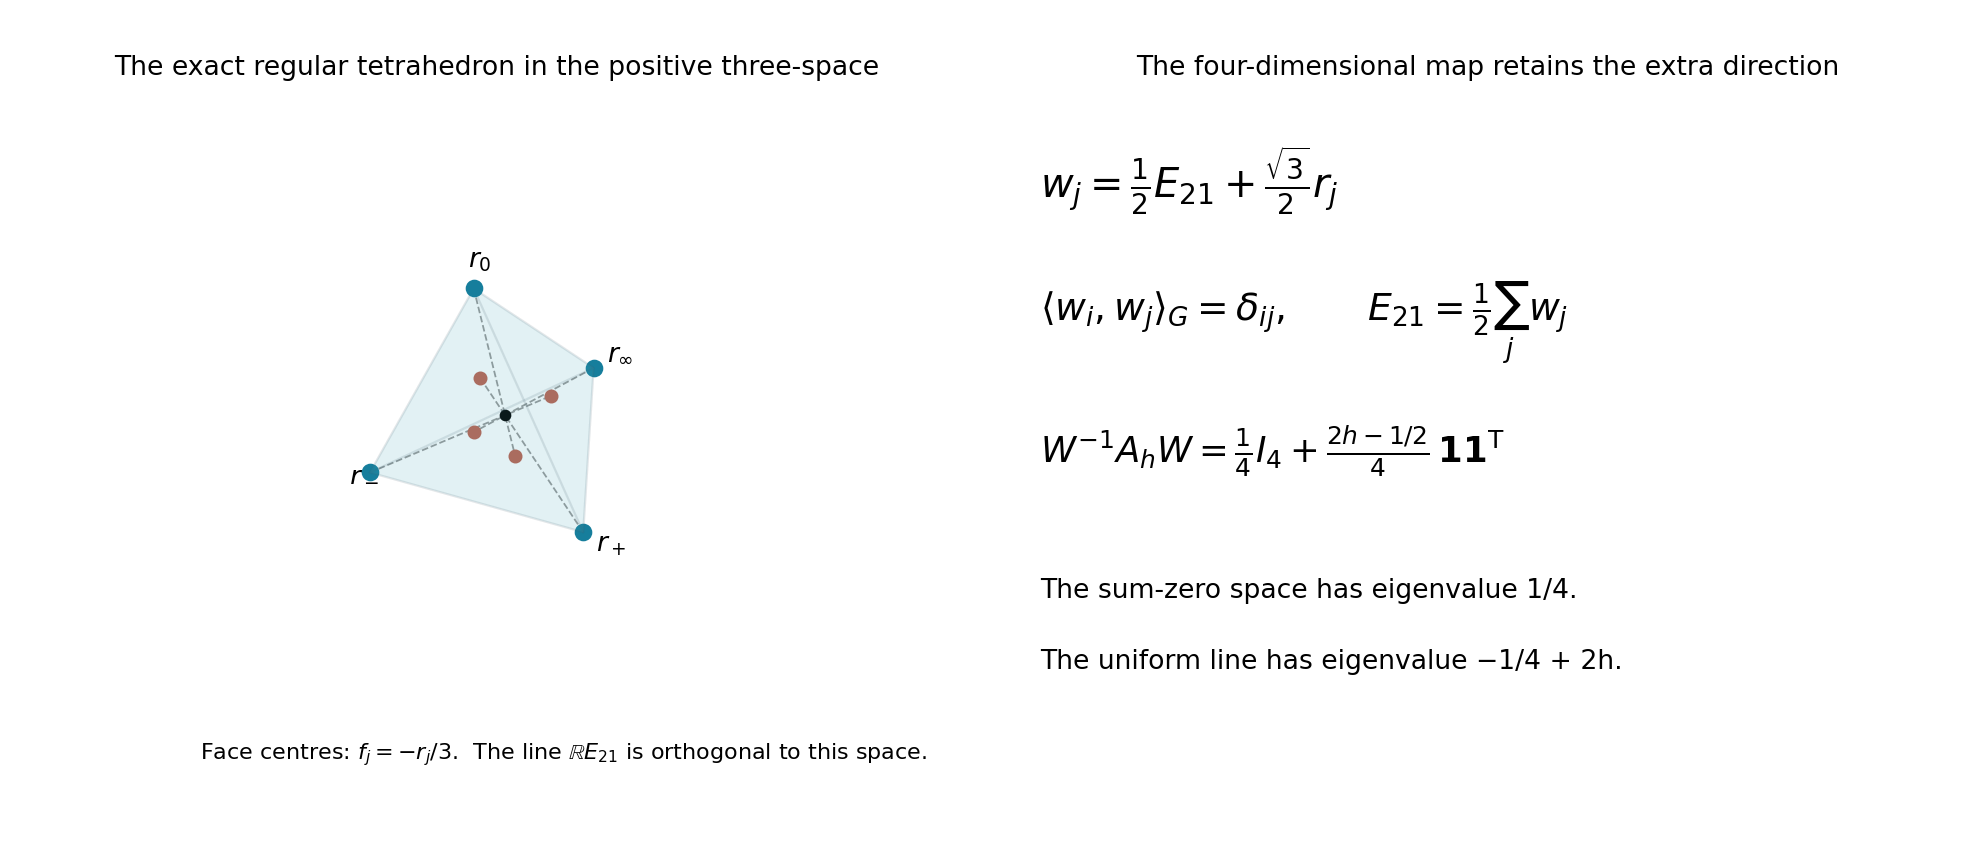
\includegraphics[keepaspectratio,alt={Exact tetrahedral vertices and face centres, with the four-dimensional orthonormal frame. ESQ45--ESQ54 prove the coordinates and the uniform changing direction; the orthogonal E21 direction is retained outside the displayed three-space.}]{figures/27_tetrahedral_heat_frame.png}}
\caption{Exact tetrahedral vertices and face centres, with the
four-dimensional orthonormal frame. ESQ45--ESQ54 prove the coordinates
and the uniform changing direction; the orthogonal E21 direction is
retained outside the displayed three-space.}
\end{figure}

\clearpage

\section{The quarter heat family in the actual ES free-shell
operator}\label{the-quarter-heat-family-in-the-actual-es-free-shell-operator}

23 September 2026. This note transports the quarter family through the
spectral projectors of the actual raw ES operator into its free-shell
carrier. It retains the original forced metric, the full raw matrix
product, the two ordered sheets, all three rotations, every orbit label,
the ambient simplex kernel, and both directed blades. It constructs the
bounded operator on the full orbit Hilbert space, its exact quadratic
algebra receiver and collision pairing, and the full Figure 10
support-corner and modular transport. Every finite orbit compression is
compatible with these maps. No equality with a Weil distribution is
asserted.

The original source read is
\texttt{ES-\allowbreak{}Fable-\allowbreak{}C123/\allowbreak{}es\_\allowbreak{}fable\_\allowbreak{}c123\_\allowbreak{}preprint.\allowbreak{}tex}. The precise inputs
are \texttt{eq:\allowbreak{}raw-\allowbreak{}negative-\allowbreak{}cell-\allowbreak{}projector},
\texttt{eq:\allowbreak{}raw-\allowbreak{}positive-\allowbreak{}cell-\allowbreak{}projector},
\texttt{eq:\allowbreak{}pulled-\allowbreak{}back-\allowbreak{}quarter-\allowbreak{}cell-\allowbreak{}signs},
\texttt{thm:\allowbreak{}quarter-\allowbreak{}three-\allowbreak{}plus-\allowbreak{}one},
\texttt{eq:\allowbreak{}origin-\allowbreak{}resolved-\allowbreak{}support}, \texttt{eq:\allowbreak{}origin-\allowbreak{}involution},
\texttt{eq:\allowbreak{}star-\allowbreak{}kneser-\allowbreak{}D3-\allowbreak{}cover-\allowbreak{}hypotheses},
\texttt{thm:\allowbreak{}general-\allowbreak{}shell-\allowbreak{}123-\allowbreak{}linking-\allowbreak{}decomposition},
\texttt{cor:\allowbreak{}general-\allowbreak{}shell-\allowbreak{}simplex-\allowbreak{}Lorentz-\allowbreak{}pullback}, and
\texttt{thm:\allowbreak{}general-\allowbreak{}shell-\allowbreak{}control-\allowbreak{}determinant-\allowbreak{}volume}. The corresponding
public reading edition is
\href{https://github.com/KokunoYumeto/erdos-straus-foundation/blob/20709bee872ad10e4cc7d7b976d975e24532a803/00_ERDOS_STRAUSS_Project_Reader.pdf}{\emph{Erdős--Straus
Project Reader}, pinned edition 20709bee}. The mathematical reading for
this derivation used the original TeX, not extracted PDF text. All
finite and infinite operator claims below are proved here from the
explicit source matrices and labels.

\subsection{1. The original arithmetic labels and the actual shell
spaces}\label{the-original-arithmetic-labels-and-the-actual-shell-spaces}

For the ES source, let \(p\) be a prime, let \(a_{\rm ar}\) be a
positive integer, and retain \[
R=4a_{\rm ar}-p>2,\qquad\gcd(R,pa_{\rm ar})=1,
\qquad N=pa_{\rm ar}.
\tag{ESHL1}
\] These are \texttt{eq:\allowbreak{}star-\allowbreak{}kneser-\allowbreak{}D3-\allowbreak{}cover-\allowbreak{}hypotheses}. They imply
that \(p\) is odd and \(p\nmid a_{\rm ar}\): for \(p=2\), \(R\) and
\(pa_{\rm ar}\) are both even; for odd \(p\mid a_{\rm ar}\), the same
prime divides \(R\). Define exactly the origin-resolved set \[
\mathcal X_{R,p}=
\{(j,u):j\in\{0,1,2\},\ u\mid a_{\rm ar}^2,
\quad u a_{\rm ar}^{-1}=-p^{1-j}\text{ in }(\mathbb Z/R\mathbb Z)^\times\}.
\tag{ESHL2}
\] All inverses in this formula exist by ESHL1. Its involution is \[
\iota(j,u)=(2-j,a_{\rm ar}^2/u).
\tag{ESHL3}
\] It preserves the defining congruence because taking its
multiplicative inverse turns \(-p^{1-j}\) into \(-p^{j-1}\). Applying it
twice gives the identity. A fixed point would have \(j=1,u=a_{\rm ar}\);
the congruence would then give \(1=-1\pmod R\), impossible for \(R>2\).
Thus all its orbits have size two.

Let \(\mathcal O=\mathcal X_{R,p}/\langle\iota\rangle\) and
\(q=|\mathcal O|\). The two divisors \(d(j,u)=p^ju\) in any orbit have
product \(N^2\). They are unequal: uniqueness of the representation
\(p^ju\), using \(p\nmid a_{\rm ar}\), would otherwise give a fixed
point of \(\iota\). Thus each orbit has a unique low member \(x_O^-\)
with divisor below \(N\) and high member \(x_O^+\) with divisor above
\(N\). This proves the original ordering used by the source.

The complete free-cover labels are \((O,\epsilon,m)\), where
\(\epsilon\in\{0,1\}\) names the low/high sheet and
\(m\in\mathbb Z/3\mathbb Z\) names the rotation. The original bijection
and its unitary linearization are \[
\theta_{123}(m,x_O^\epsilon)=(O,\epsilon,m),
\quad
\Theta_{123}:\mathbb C[\widetilde{\mathcal X}_{R,p}]
\longrightarrow \mathcal H_q:=\mathbb C[\mathcal O]\otimes\mathbb C^2\otimes\mathbb C^3,
\quad e_{(m,x_O^\epsilon)}\mapsto e_O\otimes f_\epsilon\otimes g_m.
\tag{ESHL4}
\] They are bijections because the three labels recover the original
point. The map is unitary for the stated orthonormal label bases. Hence
\(\dim\mathcal H_q=6q\), retaining every label.

Let \(P_2=I_3-\mathbf1\mathbf1^*/3\) be the source triangle support
projector. The original support unitary
\(\mathsf U_2:\operatorname{Ran}P_2\to\mathbb C^2\) satisfies
\(\mathsf U_2^*\mathsf U_2=P_2\) and \(\mathsf U_2\mathsf U_2^*=I_2\),
as proved in \texttt{eq:\allowbreak{}simplex-\allowbreak{}123-\allowbreak{}unitary-\allowbreak{}identities}. Write
\(\eta_\epsilon=\mathsf U_2^*f_\epsilon\). These are an orthonormal
basis of the original triangle support, with their original coordinate
choice retained. The actual ambient simplex space and its support are \[
\mathcal K_q=\mathbb C[\mathcal O]\otimes\mathbb C^3\otimes\mathbb C^3,
\qquad
\mathcal H_q^{\rm simp}=\mathbb C[\mathcal O]\otimes\operatorname{Ran}P_2\otimes\mathbb C^3.
\tag{ESHL5}
\] The isometry \(V_q=I\otimes\mathsf U_2^*\otimes I_3\) identifies
\(\mathcal H_q\) with \(\mathcal H_q^{\rm simp}\). Its range projector
is \(P_q^{\rm simp}=I\otimes P_2\otimes I_3\). The retained
complementary space is \[
\mathcal Z_q=\mathbb C[\mathcal O]\otimes\mathbb C\mathbf1\otimes\mathbb C^3,
\quad\mathcal K_q=\mathcal H_q^{\rm simp}\oplus\mathcal Z_q,
\quad\dim\mathcal Z_q=3q.
\tag{ESHL6}
\] This ambient kernel is different from the source map \(\Pi_{123}\),
which sends all six labels in an orbit to one support label and has
kernel dimension \(5q\). Explicitly that latter kernel is the subspace
whose six coefficients sum to zero on every orbit. Neither of these
kernels is substituted for the other.

\subsection{2. The raw quarter operator and its spectral
algebra}\label{the-raw-quarter-operator-and-its-spectral-algebra}

Give the raw four-cell vector space
\(\mathcal V_{\rm raw}=M_2(\mathbb C)\) its Hilbert--Schmidt inner
product, with orthonormal basis \(E_{11},E_{12},E_{21},E_{22}\). The
original forced ES metric is retained by the explicit isometry
ESHL43--ESHL44 below. The source's pulled-back quarter reflection acts
by \[
\mathfrak Q_\square(E_{11})=E_{11},\quad
\mathfrak Q_\square(E_{12})=E_{12},\quad
\mathfrak Q_\square(E_{21})=-E_{21},\quad
\mathfrak Q_\square(E_{22})=E_{22}.
\tag{ESHL7}
\] Consequently its orthogonal spectral projectors are \[
P_-(M)=M_{21}E_{21},\qquad P_+=I_{\mathcal V_{\rm raw}}-P_-.
\tag{ESHL8}
\] They satisfy \(P_\pm^2=P_\pm=P_\pm^*\), \(P_+P_-=0\), with ranks
three and one. Define the exact raw quarter operator and its heat family
by \[
A_0=\tfrac14P_+-\tfrac14P_-,\qquad
A_h=\tfrac14P_++a(h)P_-,\qquad a(h)=-\tfrac14+2h.
\tag{ESHL9}
\] The original coefficient inversion matrix \(\mathcal I_-\) is
transported to this raw presentation by the source map
\(\mathcal T_\square\), since \texttt{eq:\allowbreak{}pulled-\allowbreak{}back-\allowbreak{}quarter-\allowbreak{}reflection}
states
\(\mathfrak Q_\square=\mathcal T_\square^{-1}(4\mathcal I_-)\mathcal T_\square\).
Thus \(A_0\) is the actual pulled-back quarter operator.

The fixed spectral algebra is \[
\mathcal D=\mathbb C[A_0]
=\{cP_++dP_-:c,d\in\mathbb C\}\cong\mathbb C^2.
\tag{ESHL10}
\] Indeed \(P_+=2A_0+I/2\), \(P_-=-2A_0+I/2\), so both projectors belong
to the generated algebra. Their orthogonality proves multiplication is
coordinatewise and the involution conjugates \(c,d\). The representation
is faithful because both projectors have nonzero range.

The original forced metric in \texttt{eq:\allowbreak{}Fable-\allowbreak{}forced-\allowbreak{}full-\allowbreak{}metric}, also
used in ESQ9, has matrix \[
G=\begin{pmatrix}
1/16&0&0&-7/144\\
0&2/9&0&0\\
0&0&1&0\\
-7/144&0&0&1/16
\end{pmatrix}.
\tag{ESHL43}
\] Let \(v_+=(E_{11}+E_{22})/\sqrt2\), \(v_-=(E_{11}-E_{22})/\sqrt2\),
and let \(\Pi_+,\Pi_-,\Pi_{12},\Pi_{21}\) be the Hilbert--Schmidt
projections on these two unit vectors and on \(E_{12},E_{21}\),
respectively. Multiplying ESHL43 by these four vectors gives the
respective eigenvalues \(1/72,1/9,2/9,1\). Hence the fully specified
positive square root is \[
T=G^{1/2}=\frac1{6\sqrt2}\Pi_++\frac13\Pi_-
 +\frac{\sqrt2}{3}\Pi_{12}+\Pi_{21},\qquad
T^*T=G,\qquad TP_\pm=P_\pm T,\qquad TA_h=A_hT.
\tag{ESHL44}
\] The four orthogonal projections sum to the identity. Squaring their
positive coefficients proves \(T^*T=G\), and replacing the coefficients
by their reciprocals defines the inverse. Each projection preserves the
decomposition into \(\operatorname{Ran}P_+\) and
\(\operatorname{Ran}P_-\), proving both commutation identities. Thus
\(T:(\mathcal V_{\rm raw},\langle x,Gy\rangle_{\rm HS})\to(\mathcal V_{\rm raw},\langle x,y\rangle_{\rm HS})\)
is an isometry, and the original heat form is exactly
\(\langle x,GA_hy\rangle_{\rm HS}=\langle Tx,A_hTy\rangle_{\rm HS}\).
Conjugation by \(T\) fixes every member of the spectral algebra
\(\mathcal D\). This is a vector-metric transport, and does not change
the raw matrix product: for example \(T(I_2)=I_2/(6\sqrt2)\), so \(T\)
is not a unital algebra map. The separate map preserving that product is
ESHL45.

The spectral algebra \(\mathcal D\) consists of endomorphisms of the raw
four-cell vector space. Its negative projector is the two-sided corner
operation \(P_-(X)=E_{22}XE_{11}\), as direct entry multiplication
proves. It is not a left multiplication operator: \(P_-\) has rank one,
whereas left multiplication by a nonzero rank-one matrix on
\(M_2(\mathbb C)\) has rank two, since each of two columns independently
ranges over a fixed one-dimensional image. Section 3 uses the spectral
algebra as its domain; ESHL45--ESHL47 construct the full raw matrix
algebra map and intertwine this corner operation exactly.

\subsection{3. The faithful spectral lift into the actual ordered
sheets}\label{the-faithful-spectral-lift-into-the-actual-ordered-sheets}

In \(\mathcal H_q\), define the original low and high projectors \[
Q_<=I_{\mathbb C[\mathcal O]}\otimes E_{11}^{(2)}\otimes I_3,
\qquad Q_>=I_{\mathbb C[\mathcal O]}\otimes E_{22}^{(2)}\otimes I_3.
\tag{ESHL11}
\] They are exactly \texttt{eq:\allowbreak{}general-\allowbreak{}shell-\allowbreak{}ordered-\allowbreak{}sheet-\allowbreak{}projectors}
under ESHL4. Their ranges are orthogonal, they sum to the identity on
\(\mathcal H_q\), and each has dimension \(3q\). For \(q\ge1\), define
\[
\boxed{\Psi_q:\mathcal D\longrightarrow B(\mathcal H_q),
\qquad cP_++dP_-\longmapsto cQ_<+dQ_>.}
\tag{ESHL12}
\] This is a faithful unital \(*\)-homomorphism. Orthogonality gives
\((cQ_<+dQ_>)(c'Q_<+d'Q_>)=cc'Q_<+dd'Q_>\), matching the source product.
Adjoints conjugate the same two coefficients. The source unit maps to
\(Q_<+Q_>=I\). If an image vanishes, applying it to any low and any high
basis vector gives \(c=d=0\). This proves faithfulness and also the
isometry \(\|\Psi_q(cP_++dP_-)\|=\max(|c|,|d|)\).

The map retains the two spectral labels, but changes their
representation multiplicities. Its exact trace comparison is \[
\operatorname{Tr}_{\rm raw}(cP_++dP_-)=3c+d,
\qquad \operatorname{Tr}_{\mathcal H_q}\Psi_q(cP_++dP_-)=3q(c+d).
\tag{ESHL13}
\] Thus this is not a trace-preserving or Hilbert-space unitary
identification of the four-cell space with the shell. Both multiplicity
lists remain explicit. When \(q=0\), the shell space and all its
operators are zero; the resulting map is zero and is not faithful. The
nonzero-shell assertion has therefore not been extended to an empty
arithmetic shell.

Define the fixed positive weight and its inverse on the support by \[
W=16Q_<+4Q_>,\qquad W^{-1}=\tfrac1{16}Q_<+\tfrac14Q_>.
\tag{ESHL14}
\] Both are verified by multiplication. The weight commutes with
\(\Psi_q(\mathcal D)\), and its positive square root is \(4Q_<+2Q_>\).
The lifted heat carrier is \[
\boxed{H_h:=W\Psi_q(A_h)=4Q_<+t(h)Q_>,
\qquad t(h)=-1+8h.}
\tag{ESHL15}
\] At zero it equals the actual ES carrier \[
H_0=I_{\mathbb C[\mathcal O]}\otimes\operatorname{diag}(4,-1)\otimes I_3
=H^{\rm sh}_{R,p},
\tag{ESHL16}
\] in the source's unitary presentation
\texttt{eq:\allowbreak{}general-\allowbreak{}shell-\allowbreak{}restricted-\allowbreak{}Lorentz-\allowbreak{}carrier}. The map
\(A\mapsto W\Psi_q(A)\) is a specified positive linear map on
self-adjoint elements, since it also equals \(W^{1/2}\Psi_q(A)W^{1/2}\);
it is not asserted to be an algebra homomorphism. The faithful
homomorphism is \(\Psi_q\) itself.

The original simplex presentation is \(\widetilde H_h=V_qH_hV_q^*\) on
\(\mathcal K_q\), with zero action on \(\mathcal Z_q\). This gives the
exact commuting relation \(\widetilde H_hV_q=V_qH_h\), and the
support-corner homomorphism \(D\mapsto V_q\Psi_q(D)V_q^*\) has unit
\(P_q^{\rm simp}\). It is unital as a map to that corner, not to the
whole ambient algebra with identity \(I_{\mathcal K_q}\).

\subsection{4. Positivity, the sharp gap, and every
kernel}\label{positivity-the-sharp-gap-and-every-kernel}

For \(x=x_<+x_>\) in the orthogonal sheet decomposition, \[
\langle x,H_hx\rangle=4\|x_<\|^2+t(h)\|x_>\|^2.
\tag{ESHL17}
\] Thus for a nonempty finite shell \[
\operatorname{inertia}(H_h)=
\begin{cases}
(3q,3q,0),&h<1/8,\\
(3q,0,3q),&h=1/8,\\
(6q,0,0),&h>1/8.
\end{cases}
\tag{ESHL18}
\] In particular \(H_h\succeq0\) exactly for \(h\ge1/8\). For \(h>1/8\),
the sharp lower and upper bounds are \[
\boxed{\min(4,-1+8h)I\preceq H_h
\preceq\max(4,-1+8h)I.}
\tag{ESHL19}
\] Both constants are attained on the appropriate sheet vectors in
ESHL17. The lower bound is independent of \(q\). At the critical time,
the kernel on the shell is exactly \(\operatorname{Ran}Q_>\).

On the full simplex ambient space, the kernel is \(\mathcal Z_q\) for
\(h\ne1/8\), and is \[
\ker\widetilde H_{1/8}=\mathcal Z_q\oplus V_q\operatorname{Ran}Q_>,
\quad\dim\ker\widetilde H_{1/8}=6q.
\tag{ESHL20}
\] The original ambient kernel has not disappeared when the support form
becomes positive. The sharp lower bound on the ambient space is the
support inequality \(\widetilde H_h\succeq\min(4,t(h))P_q^{\rm simp}\)
for \(h>1/8\); strict positivity is a statement on
\(\mathcal H_q^{\rm simp}\).

There are also two distinct times at which a single operator loses its
ability to recover the fixed spectral labels. At \(h=1/4\), \(A_h=I/4\),
so \(\mathbb C[A_h]=\mathbb CI\) although the fixed algebra
\(\mathcal D\) and its \(P_\pm\) remain. At \(h=5/8\), \(H_h=4I\), so
its generated algebra is scalar although \(Q_<,Q_>\) remain present.
These follow by equating their two coefficients. The lift uses
\(\mathcal D=\mathbb C[A_0]\) and the retained labelled projectors
throughout; it does not reconstruct them from the possibly scalar single
operator at these times.

\subsection{5. The actual mixed blades remain
nonzero}\label{the-actual-mixed-blades-remain-nonzero}

Retain exactly the directed blades of
\texttt{eq:\allowbreak{}general-\allowbreak{}shell-\allowbreak{}low-\allowbreak{}high-\allowbreak{}blade-\allowbreak{}transport} and
\texttt{eq:\allowbreak{}general-\allowbreak{}shell-\allowbreak{}high-\allowbreak{}low-\allowbreak{}blade-\allowbreak{}transport}: \[
D=I\otimes2E_{21}^{(2)}\otimes I_3,
\qquad U=I\otimes2E_{12}^{(2)}\otimes I_3=D^*.
\tag{ESHL21}
\] Here \(D\) is the original low-to-high sheet map and \(U\) its
adjoint; these symbols do not denote the amplitude multiplier from a
different packet calculation. Matrix-unit multiplication proves \[
D^2=U^2=0,\qquad UD=4Q_<,\qquad DU=4Q_>,
\quad\|D\|=\|U\|=2.
\tag{ESHL22}
\] Their norms follow because each takes a unit vector in its source
sheet to a vector of norm two and kills the other sheet. They are
nonzero for \(q\ge1\), at every heat time. Their precise source and
target spaces are \[
D:\operatorname{Ran}Q_<\to\operatorname{Ran}Q_>,
\qquad U:\operatorname{Ran}Q_>\to\operatorname{Ran}Q_<.
\tag{ESHL23}
\] The carrier consequently retains the original directed expression \[
H_h=UD+t(h)Q_>.
\tag{ESHL24}
\] At \(h=0\), this is exactly
\texttt{eq:\allowbreak{}general-\allowbreak{}shell-\allowbreak{}directed-\allowbreak{}Gram-\allowbreak{}support-\allowbreak{}carrier}. At \(h=1/8\),
the high sheet becomes the carrier's kernel, but \(D\) still takes the
positive sheet onto that kernel and \(U\) takes it back. The commutators
are \[
[H_h,D]=(t(h)-4)D,\qquad [H_h,U]=(4-t(h))U.
\tag{ESHL25}
\] Both follow by multiplying the two diagonal coefficients with the two
matrix units. Thus the mixed maps have not been discarded by
diagonalizing the form.

Their generated algebra is exactly \[
I_{\mathbb C[\mathcal O]}\otimes M_2(\mathbb C)\otimes I_3:
\quad E_{11}\mapsto Q_<,\ E_{22}\mapsto Q_>,
\ E_{21}\mapsto D/2,\ E_{12}\mapsto U/2.
\tag{ESHL26}
\] The four matrix-unit laws hold by ESHL22 and the sheet actions;
independence follows by applying a proposed relation to one low and one
high vector. This is an actual copy of the raw matrix algebra
\(M_2(\mathbb C)\), with its diagonal subalgebra containing
\(\Psi_q(\mathcal D)\). The faithful algebra isomorphism onto this image
is \(R_q\) in ESHL45. Section 2 identifies the spectral projector
\(P_-\) with a two-sided corner operation on that algebra; it does not
exclude the matrix algebra identification.

There is a faithful dual-number receiver
\(\mathbb C[\eta]/\eta^2\to B(\mathcal H_q)\), \(1\mapsto I\),
\(\eta\mapsto D\). Its multiplicativity follows from \(D^2=0\); applying
\(cI+dD=0\) first to a high vector and then to a low vector proves
injectivity. These nilpotents are present in the mixed operator algebra
at all times. The diagonal homomorphism \(\Psi_q\) does not itself
create a nilpotent in its reduced domain \(\mathbb C^2\).

The original rotation acts only on the third factor and commutes with
\(D,U,H_h\). The original reflection swaps the two sheet factors and
reverses rotation labels, giving \[
\mathbf S D\mathbf S^{-1}=U,
\quad\mathbf S Q_<\mathbf S^{-1}=Q_>,
\quad\mathbf S H_h\mathbf S^{-1}=t(h)Q_<+4Q_>.
\tag{ESHL27}
\] These follow directly from the source label action in
\texttt{eq:\allowbreak{}general-\allowbreak{}shell-\allowbreak{}123-\allowbreak{}label-\allowbreak{}action}. The directed carrier is
invariant under that reflection only when \(t(h)=4\). Its exact
reflected partner, rather than an unproved invariance, is retained in
ESHL27.

\subsection{6. Exact finite traces, lengths, and determinant
ratios}\label{exact-finite-traces-lengths-and-determinant-ratios}

For finite \(q\ge1\), the two eigenvalues and their multiplicities give
\[
\operatorname{Tr}H_h=3q(4+t),\quad
\|H_h\|_{\rm HS}^2=3q(16+t^2),\quad
\det H_h=4^{3q}t^{3q},
\quad t=-1+8h.
\tag{ESHL28}
\] The Hilbert--Schmidt formula is the trace of the square because
\(H_h\) is Hermitian. The determinant is the product of all eigenvalues,
including its sign. For \(t\ne0\), its absolute determinant volume and
the exact ratio to the original carrier are \[
V_h^{\det}=|4t|^{3q},\qquad
\frac{V_h^{\det}}{V_0^{\det}}=|t|^{3q},
\qquad \det(H_hH_0^{-1})=(-t)^{3q}=(1-8h)^{3q}.
\tag{ESHL29}
\] The last formula follows also from \(H_hH_0^{-1}=Q_<-tQ_>\). At the
critical time the determinant is zero; no logarithm of that zero is
treated as finite.

The exact traceless part is \[
K_h=H_h-\frac{4+t}{2}I
=\frac{4-t}{2}(Q_<-Q_>),
\qquad \|K_h\|_{\rm HS}^2=\frac{3q}{2}(4-t)^2.
\tag{ESHL30}
\] For the constant-generator paths \(\exp(-i\sigma H_h)\),
\(\exp(-i\sigma K_h)\), \(0\le\sigma\le1\), the Hilbert--Schmidt speed
is the norm of the generator: multiplying the derivative by the inverse
unitary removes the unitary factor and leaves the same Hilbert--Schmidt
norm. Thus their squared lengths equal the two squared norms in ESHL28
and ESHL30. At \(h=0\) they are \(51q\) and \(75q/2\), exactly the ES
source constants.

All per-orbit quantities have exact finite formulas, with the full
factor \(q\) retained: \[
\frac{\operatorname{Tr}H_h}{q}=3(4+t),\quad
\frac{\|H_h\|_{\rm HS}^2}{q}=3(16+t^2),\quad
\frac{\log V_h^{\det}}q=3\log|4t|\quad(t\ne0).
\tag{ESHL31}
\] For \(t\ne0\), these imply \[
\log V_h^{\det}
=\frac{\log|4t|}{16+t^2}\|H_h\|_{\rm HS}^2.
\tag{ESHL32}
\] For \(t\ne0,4\), they also imply \[
\log V_h^{\det}
=\frac{2\log|4t|}{(4-t)^2}\|K_h\|_{\rm HS}^2.
\tag{ESHL33}
\] At \(t=-1\), these coefficients are \(2\log2/17\) and \(4\log2/25\),
reproducing the original determinant-length identities. At \(t=4\),
\(K_h=0\) while \(V_h^{\det}=16^{3q}\), so the second quotient is not
defined; the original exact formulas still apply. This handles the
exceptional scalar carrier explicitly.

\subsection{7. The actual infinite orbit-space
operator}\label{the-actual-infinite-orbit-space-operator}

Let \(\mathcal O_\infty\) be any nonempty countable set of the retained
labelled complement orbits, with shell labels included when orbits from
different shells are combined. The empty case is the zero space already
specified after ESHL13. Form the actual Hilbert completion \[
\mathcal H_\infty=\ell^2(\mathcal O_\infty)\otimes\mathbb C^2\otimes\mathbb C^3.
\tag{ESHL34}
\] This definition also covers a finite orbit set. If it is infinite,
the following statements concern that same labelled Hilbert space; no
assertion that every arithmetic shell is occupied is being introduced.
The projectors \(Q_<,Q_>\), blades \(D,U\), weight \(W\), and
\(\Psi_\infty\) are defined by the identical tensor formulas
ESHL11--ESHL15 and ESHL21.

For example, if \(x=(x_{O,<,m},x_{O,>,m})\), then \[
(H_hx)_{O,<,m}=4x_{O,<,m},\qquad
(H_hx)_{O,>,m}=t(h)x_{O,>,m}.
\tag{ESHL35}
\] The square sum of these coordinates is bounded by
\(\max(16,t(h)^2)\|x\|^2\), proving that \(H_h\) is everywhere defined
and bounded. Choosing a single sheet basis vector proves \[
\|H_h\|=\max(4,|t(h)|),\qquad
\|H_h-H_{h'}\|=8|h-h'|.
\tag{ESHL36}
\] Its adjoint is itself by the real diagonal coefficients. Its
quadratic form is the convergent sum of ESHL17 over all labels, so the
positivity criterion and sharp uniform lower bound ESHL19 remain valid
without a dimension-dependent error. In particular, for every fixed
\(h>1/8\), \(H_h\) is boundedly invertible on the entire orbit support,
with \[
H_h^{-1}=\tfrac14Q_<+\frac1{t(h)}Q_>,
\qquad\|H_h^{-1}\|=\frac1{\min(4,t(h))}.
\tag{ESHL37}
\] This is an explicit inverse, verified by multiplication. At
\(h=1/8\), its kernel is the whole high-sheet Hilbert subspace and its
range is the low-sheet subspace. The blades remain bounded with norm two
and retain every identity ESHL22--ESHL27.

The infinite ambient simplex space is
\(\mathcal K_\infty=\ell^2(\mathcal O_\infty)\otimes\mathbb C^3\otimes\mathbb C^3\).
Its orthogonal decomposition is the completed version of ESHL5--ESHL6,
and \(V_\infty=I\otimes\mathsf U_2^*\otimes I_3\) gives the same
isometry and support projector. The zero action on the entire
complementary Hilbert space is retained, including when \(H_h\) is
uniformly positive on its support.

For completeness, every local matrix unit also remains an actual bounded
operator. For basis labels \(\alpha=(O,\epsilon,m)\),
\(\beta=(O',\epsilon',m')\), define \[
E_{\alpha\beta}x=e_\alpha\langle e_\beta,x\rangle.
\tag{ESHL38}
\] Its norm is one, its adjoint is \(E_{\beta\alpha}\), and
\(E_{\alpha\beta}E_{\gamma\delta}=\delta_{\beta\gamma}E_{\alpha\delta}\),
all by direct application to a vector. Thus the mixed maps, including
maps between different orbit labels, are present in
\(B(\mathcal H_\infty)\). The particular global blades are the strong
sums \(D=2\sum_{O,m}E_{(O,>,m),(O,<,m)}\) and its adjoint, whose
orthogonal source and target coordinates give norm two.

\subsection{8. Exact compatibility with all finite
compressions}\label{exact-compatibility-with-all-finite-compressions}

For a finite subset \(F\subset\mathcal O_\infty\), take all two-sheet
and three-rotation labels over its orbits. Let
\(j_F:\mathcal H_F\to\mathcal H_\infty\) be inclusion by zero outside
\(F\), and \(P_F=j_Fj_F^*\). It is an isometry. The tensor formulas give
\[
H_hj_F=j_FH_{h,F},\quad j_F^*H_hj_F=H_{h,F},
\quad P_FH_h=H_hP_F,
\quad\Psi_\infty(A)j_F=j_F\Psi_F(A).
\tag{ESHL39}
\] The same equations hold for \(D,U,W\) and the original rotation and
reflection operators because none changes the orbit label. Thus these
are the actual finite lifts and their exact inclusions, not new finite
approximations with altered sheets or rotations.

For nested finite orbit sets \(F_n\) exhausting \(\mathcal O_\infty\),
the square-summable tail identity gives \(\|(I-P_{F_n})x\|\to0\) for
every \(x\). Therefore \[
P_{F_n}H_hP_{F_n}\longrightarrow H_h
\quad\text{strongly on }\mathcal H_\infty.
\tag{ESHL40}
\] Indeed the difference on \(x\) has norm at most
\(\|H_h\|\|(I-P_{F_n})x\|\), since the projections commute with \(H_h\).
Positivity and its uniform bound already hold on every finite
compression and on the limiting operator by ESHL17; there is no hidden
loss of the lower bound in this limit. If every \(F_n\) has a nonempty
complement, this convergence is not in operator norm: a unit tail vector
in a sheet attaining the maximum eigenvalue magnitude has difference
norm \(\max(4,|t(h)|)\). The exact topology of convergence is thereby
specified.

\subsection{9. Infinite traces and the retained finite-volume
data}\label{infinite-traces-and-the-retained-finite-volume-data}

When \(\mathcal O_\infty\) is infinite, \(H_h\) is never
Hilbert--Schmidt: its value on each of infinitely many low-sheet basis
vectors has norm four, so the sum of their squared norms diverges. It is
not trace class for the same reason, since \(|H_h|\) has eigenvalue four
infinitely often. For \(h\ge1/8\), its extended positive trace is
\(+\infty\). For \(h<1/8\), its positive and negative parts both have
infinite trace, so an ordinary signed trace would be the undefined
difference \(\infty-\infty\). None of these facts changes its bounded
operator norm or the positive lower bound at \(h>1/8\).

The ordinary finite-dimensional determinant has no direct
infinite-dimensional value here. More precisely, for \(h\ne0\), the
relative operator is \[
H_hH_0^{-1}=I-8hQ_>.
\tag{ESHL41}
\] Its difference from the identity is not compact: it takes an infinite
orthonormal sequence in the high sheet to an orthogonal sequence of
fixed nonzero norm. Hence that difference is not trace class, and the
usual trace-class Fredholm determinant is unavailable. At \(h=0\) the
relative operator is the identity and its determinant is one.

The exact finite determinants and per-orbit data remain ESHL28--ESHL33
on every finite subset. Their absolute values can tend to zero,
infinity, or remain one, depending on \(|4t(h)|\); none of those
sequence behaviours alone defines an ordinary determinant of the
infinite operator. On the specified constant-fibre algebra
\(I_{\ell^2(\mathcal O_\infty)}\otimes M_6(\mathbb C)\), there is
instead the exact finite fibre trace
\(\tau_{\rm fibre}(I\otimes B)=\operatorname{Tr}_{\mathbb C^6}B\). It
equals \(\operatorname{Tr}_{\mathcal H_F}(j_F^*(I\otimes B)j_F)/|F|\) on
every nonempty finite orbit set. Thus, for \(t(h)\ne0\), the explicitly
defined fibre determinant is \[
\exp\bigl(\tau_{\rm fibre}(\log|H_h|)\bigr)=|4t(h)|^3.
\tag{ESHL42}
\] This is a finite-fibre observable with its exact comparison map; it
is not presented as an ordinary infinite determinant. The full orbit
labels, all local injections, the fixed spectral representation, and the
ambient kernel remain in the construction.

The result is a lift of the stated quarter heat family into the actual
ES free-shell carrier, with a bounded infinite-orbit extension and a
uniform positive support bound after \(h=1/8\). The full raw
multiplication and quadratic receiver are constructed in ESHL45--ESHL50,
the collision pairing in ESHL51--ESHL53, and the complete Figure 10
transport in ESHL54--ESHL64. These maps do not identify the ES spectral
algebra or its infinite orbit trace with an arithmetic Weil pairing.

\subsection{10. Exact finite
verification}\label{exact-finite-verification-1}

The reproducible script \texttt{check\_\allowbreak{}es\_\allowbreak{}shell\_\allowbreak{}heat\_\allowbreak{}lift.\allowbreak{}py} passed
\textbf{217 exact symbolic checks}, recorded in
\texttt{ES\_\allowbreak{}SHELL\_\allowbreak{}HEAT\_\allowbreak{}LIFT\_\allowbreak{}CHECKS.\allowbreak{}json}. They verify the raw
spectral projectors and their multiplicities, the original forced metric
isometry, the full raw matrix product and corner operation, the
quadratic receiver and its original involution, the complete collision
pairing, both blade products and nilpotence, all stated trace and
determinant formulas, the original control-length constants, and the
ambient kernel dimensions for one, two, and three complete orbit blocks.
They also check finite inclusions retaining all six labels per orbit;
the original displayed segment, triangle, and tetrahedron synthesis
matrices; all nine rectangular corners and their 27 typed compositions;
all 36 density ratios; the full Hilbert--Schmidt map; inter-orbit
transport; and the exact ambient multiplicativity defect. The bounded
infinite extension, its sharp lower bound, and strong convergence are
proved in ESHL34--ESHL40 and ESHL62--ESHL63; they are not inferred from
the finite checks.

\subsection{11. The full raw matrix product and its exact corner
operation}\label{the-full-raw-matrix-product-and-its-exact-corner-operation}

For every nonempty finite or countable orbit set \(\mathcal O\), use its
Hilbert space
\(\mathcal H_{\mathcal O}=\ell^2(\mathcal O)\otimes\mathbb C^2\otimes\mathbb C^3\),
where \(\ell^2(\mathcal O)=\mathbb C[\mathcal O]\) when the set is
finite. Define \[
R_{\mathcal O}:M_2(\mathbb C)\longrightarrow B(\mathcal H_{\mathcal O}),
\qquad R_{\mathcal O}(X)=I_{\ell^2(\mathcal O)}\otimes X\otimes I_3.
\tag{ESHL45}
\] The tensor product laws give \(R(XY)=R(X)R(Y)\), \(R(I_2)=I\), and
\(R(X^*)=R(X)^*\). If \(R(X)=0\), fix an orbit \(O\) and rotation \(m\);
its restriction to the span of
\(e_O\otimes f_0\otimes g_m,e_O\otimes f_1\otimes g_m\) is the matrix
\(X\), so \(X=0\). This proves faithfulness. The same restriction,
together with the square-sum norm bound over all \((O,m)\), proves
\(\|R(X)\|=\|X\|\). The inverse on its image is precisely that
two-dimensional restriction for any fixed \((O,m)\), independent of the
choice. Its image is the whole blade algebra ESHL26, since it sends
\(E_{11},E_{22},E_{21},E_{12}\) to \(Q_<,Q_>,D/2,U/2\), respectively.

Entry multiplication in the original raw matrix algebra gives
\(P_-(X)=E_{22}XE_{11}\). Applying the multiplicative map just proved
gives \[
R(P_-X)=Q_>R(X)Q_<,
\qquad
R(A_hX)=\frac14R(X)+\left(a(h)-\frac14\right)Q_>R(X)Q_<.
\tag{ESHL46}
\] Thus the quarter operator acts on the blade algebra by the explicitly
displayed linear operation on operators. This is the exact relation
between the spectral endomorphism and the matrix multiplication. It is
different from left multiplication by the heat carrier \(H_h\): the
former fixes the upper-right matrix cell with coefficient \(1/4\), while
\(H_hR(E_{12})=4R(E_{12})\). Both actions are retained with their
domains and constants. The spectral lift \(\Psi(A_h)\) of ESHL12 and the
operator-valued map \(X\mapsto R(A_hX)\) of ESHL46 also have different
domains; ESHL46 is their explicitly calculated underlying raw-cell
action, not an asserted equality of those maps.

For finite \(q\), the matrix trace on \(q\) identical orbit blocks and
three identical rotation blocks gives \[
\operatorname{Tr}(R(X)^*R(Y))=3q\operatorname{tr}_2(X^*Y),
\qquad
\operatorname{Tr}(R(TX)^*R(TY))=3q\langle X,GY\rangle_{\rm HS}.
\tag{ESHL47}
\] The second equality follows from the first and \(T^*T=G\); \(TX\)
means the four-dimensional linear metric map ESHL44 applied to the raw
matrix viewed as a vector. If \(\widehat A_h\) denotes the linear
operator in the right side of ESHL46, then
\(\widehat A_hR(TY)=R(A_hTY)=R(TA_hY)\). Inserting this in ESHL47 gives
\(\operatorname{Tr}(R(TX)^*\widehat A_hR(TY))=3q\langle X,GA_hY\rangle_{\rm HS}\).
This proves the original metric and form transport alongside the
product-preserving map. For an infinite orbit set, the same formulas
with the finite fibre trace \(\tau_{\rm fibre}\) replace \(3q\) by
\(3\); the ordinary traces of these repeated operators need not be
finite.

\subsection{12. The original quadratic algebra, its involution, and the
vanishing
infinitesimal}\label{the-original-quadratic-algebra-its-involution-and-the-vanishing-infinitesimal}

For real \(a\), define \(E_a=\mathbb C[r]/(r^2+a)\), with
coefficient-conjugating involution
\((c+dr)^\#=\overline c-\overline d r\). The basis \((1,r)\) is
independent because the relation is monic of degree two. Multiplication
by \(r\) on this basis has matrix
\(\left(\begin{smallmatrix}0&-a\\1&0\end{smallmatrix}\right)\), so the
regular trace is \(\operatorname{Tr}_{E_a}(c+dr)=2c\). The original
matrix receiver, proved in ESQ36 and re-established by the following
multiplication, is \[
\begin{aligned}
\rho_a(c+dr)&=cI_2+d(E_{21}-aE_{12}),\\
\rho_{a,\mathcal O}:=R_{\mathcal O}\rho_a,\qquad
\rho_{a,\mathcal O}(c+dr)&=cI+\frac d2(D-aU),\qquad
K_{a,\mathcal O}:=\frac12(D-aU),\qquad
K_{a,\mathcal O}^2=-aI.
\end{aligned}
\tag{ESHL48}
\] For the last identity, ESHL22 gives \((D-aU)^2=-a(DU+UD)=-4aI\).
Therefore the coefficient product is \((c,d)(e,f)=(ce-adf,cf+de)\),
exactly the multiplication in \(E_a\). The unit maps to \(I\). Applying
the displayed matrix on one fixed orbit and rotation recovers \(c\) from
either diagonal entry and \(d\) from the lower-left entry; hence the map
is faithful even when \(a=0\). The map is an isomorphism onto the
explicit commutative subalgebra \(\mathbb C[I,K_{a,\mathcal O}]\), with
inverse recovering those two entries. Its constants require no division
by \(a\), so the isomorphism includes the collision. This construction
is initially defined over \(\mathbb Z[a]\), before specializing the
parameter or extending coefficients.

Let \(\mathcal C\) be coefficient conjugation in the original
orbit-sheet-rotation basis and \(J_s=Q_<-Q_>\). The symbol \(J_s\) is
the sheet-sign operator and is unrelated to the adjunction map on a
Hilbert--Schmidt space in Section 13. Both \(J_s\) and \(\mathcal C\)
square to the identity and commute. The matrix-unit actions give
\(J_sDJ_s=-D\), \(J_sUJ_s=-U\), and coefficient conjugation fixes the
matrices \(D,U\). Consequently \[
\rho_{a,\mathcal O}(p^\#)
=J_s\mathcal C\rho_{a,\mathcal O}(p)\mathcal C J_s.
\tag{ESHL49}
\] On the full operator algebra the right side defines a
conjugate-linear multiplicative order-two map: the two adjacent factors
\(\mathcal C J_sJ_s\mathcal C\) cancel in a product. It is not the
Hilbert adjoint, which reverses product order. On the commutative image
in ESHL48 it realizes exactly the source involution \(\#\);
commutativity makes both product-order descriptions agree there. These
facts prove the type of the involution without changing it to the
positive Hilbert adjoint.

In a finite shell its trace and reflected pairing retain their full
multiplicity: \[
\begin{aligned}
\operatorname{Tr}_{\mathcal H_q}\rho_{a,q}(p)&=3q\operatorname{Tr}_{E_a}(p),\\
\operatorname{Tr}_{\mathcal H_q}\bigl(\rho_{a,q}(p^\#)\rho_{a,q}(q')\bigr)
&=6q\bigl(\overline c e+a\overline d f\bigr),
\quad p=c+dr,\ q'=e+fr.
\end{aligned}
\tag{ESHL50}
\] Indeed each orbit and rotation contains the same two-dimensional
regular matrix, and \(p^\#q'\) has scalar coefficient
\(\overline c e+a\overline d f\). The finite fibre trace on an infinite
orbit space gives the same two equations with \(q=1\); this does not
turn the repeated operator into a trace-class operator. In the basis
\((1,r)\), the full finite reflected Gram matrix is
\(6q\operatorname{diag}(1,a)\). Its inertia is \((1,1,0)\) for \(a<0\),
\((1,0,1)\) for \(a=0\), and \((2,0,0)\) for \(a>0\), because the two
real diagonal entries have exactly those signs. These are the two
algebra-coordinate multiplicities, alongside the actual shell-vector
multiplicities ESHL18.

Set \(a=a(h)=-1/4+2h\); then \(t(h)=4a(h)\), so the algebra collision
and the carrier collision occur at the same original heat time
\(h=1/8\). The two maps giving them are the quadratic algebra map ESHL48
and the weighted spectral map \(H_h=W\Psi(A_h)\), respectively. They are
related by their actual common blades and the formulas already proved;
they have not been declared to be the same map. At the collision put \[
N:=\rho_{0,\mathcal O}(r)=D/2,
\quad N\ne0,\quad N^2=0,\quad
N^*N=Q_<,\quad NN^*=Q_>,\quad
H_{1/8}N=0,\quad NH_{1/8}=4N.
\tag{ESHL51}
\] The two products with \(N^*\) follow from ESHL22. In particular \(N\)
is nonzero and maps the low sheet isometrically onto the high sheet.
Multiplication by \(H_{1/8}=4Q_<\) on the left kills its high-sheet
image; multiplication on the right multiplies its low-sheet source by
four. This proves both asymmetric mixed products and proves that the
vanishing does not erase the infinitesimal.

For every pair of vectors \(v,w\) in the complete shell Hilbert space,
finite or infinite, the complete carrier pairing is \[
\begin{aligned}
\langle Nv,H_hNw\rangle
&=t(h)\langle Q_<v,Q_<w\rangle,\\
\langle Nv,H_{1/8}Nw\rangle&=0,\qquad
\langle x,H_{1/8}Nv\rangle=\langle Nv,H_{1/8}x\rangle=0
\quad\text{for every }x.
\end{aligned}
\tag{ESHL52}
\] To prove the first identity, \(H_hN=t(h)N\) by its high-sheet image,
and \(N^*N=Q_<\); hence \(N^*H_hN=t(h)Q_<\). The remaining identities
follow either by setting \(t=0\) or by using the self-adjointness of the
carrier and \(H_{1/8}N=0\). After the collision,
\(\langle Nv,H_hNv\rangle>0\) holds exactly when \(Q_<v\ne0\). Before
the collision it is strictly negative for the same nonzero source. At
the collision the original form vanishes on that whole image, whereas
its Hilbert norm is still \(\|Nv\|^2=\|Q_<v\|^2\). These formulas
specify the vanishing observable and the surviving norm in the same
coordinates.

There is also an exact regular-trace vanishing. In a finite shell, \[
\operatorname{Tr}N^j=0\ (j\ge1),\qquad
\det(I-zN)=1,\qquad
\operatorname{Tr}(N^*N)=\operatorname{Tr}(NN^*)=3q.
\tag{ESHL53}
\] For \(j=1\) the matrix diagonal is zero; for \(j\ge2\) the operator
is zero. On each two-dimensional block \(I-zN\) is triangular with both
diagonal entries one, proving the determinant, including every rotation
and orbit. The last equalities count the ranks of the two projections.
In an infinite orbit set, the fibre trace gives the corresponding values
zero and three, while \(N\) is not trace class and \(I-zN\) has no
trace-class Fredholm determinant for \(z\ne0\): its difference from the
identity sends an infinite orthonormal low-sheet sequence to an
orthogonal sequence of norm \(|z|\). Thus neither the surviving mixed
product nor the infinite trace domain is hidden by the zero regular
trace. The receiver \(\eta\mapsto D\) in Section 5 is the same collision
algebra after the explicit scalar algebra isomorphism \(\eta\mapsto2r\),
whose inverse sends \(r\mapsto\eta/2\).

\subsection{13. The full Figure 10 corner map and its modular
transport}\label{the-full-figure-10-corner-map-and-its-modular-transport}

This section reads and proves the source result
\texttt{thm:\allowbreak{}simplex-\allowbreak{}123-\allowbreak{}modular-\allowbreak{}intertwiner} displayed in Figure
\texttt{fig:\allowbreak{}simplex-\allowbreak{}123-\allowbreak{}modular-\allowbreak{}linking}. Its nine-dimensional source is
the direct sum \(\mathbb C^2\oplus\mathbb C^3\oplus\mathbb C^4\), rather
than the tensor ambient space \(\mathbb C^3\otimes\mathbb C^3\) of
ESHL5. Their exact support transport will be given below, so neither
ambient presentation is silently substituted for the other.

For \(n=1,2,3\), retain the original regular-simplex vectors
\(v_0,\ldots,v_n\) in the \(n\)-dimensional space \(V_n\): their inner
products are one on the diagonal and \(-1/n\) off the diagonal. For
\(n=1\) the two vectors are exactly \(1,-1\). Let
\(\mathsf S_n:\mathbb C^{n+1}\to V_n\) send \(e_i\) to \(v_i\), and
define \[
P_n=I_{n+1}-\frac1{n+1}\mathbf1\mathbf1^*,\qquad
\mathsf U_n=\sqrt{\frac n{n+1}}\mathsf S_nP_n,
\quad
P=P_1\oplus P_2\oplus P_3,
\quad\mathsf U=\mathsf U_1\oplus\mathsf U_2\oplus\mathsf U_3.
\tag{ESHL54}
\] The Gram entries give \(\mathsf S_n^*\mathsf S_n=(n+1)P_n/n\). Thus
\(\mathsf U_n^*\mathsf U_n=P_n\). Its rank is \(n\), equal to
\(\dim V_n\); its restriction to \(\operatorname{Ran}P_n\) is therefore
an onto isometry, proving \(\mathsf U_n\mathsf U_n^*=I_{V_n}\). It
follows that \(\mathsf U^*\mathsf U=P\),
\(\mathsf U\mathsf U^*=I_{\mathcal V}\), where
\(\mathcal V=V_1\oplus V_2\oplus V_3\) has dimension six and \(P\) has
rank six. The full ambient kernel is the direct sum of the three
constant lines \(\mathbb C\mathbf1_{n+1}\).

The full map and inverse are \[
\Phi:PM_9(\mathbb C)P\longrightarrow B(\mathcal V),\quad
\Phi(X)=\mathsf UX\mathsf U^*,\qquad
\Phi^{-1}(Y)=\mathsf U^*Y\mathsf U.
\tag{ESHL55}
\] The products of the two maps in either order reduce to \(PXP=X\) and
\(IYI=Y\). For supported \(X,Y\),
\(\Phi(X)\Phi(Y)=\mathsf UX(\mathsf U^*\mathsf U)Y\mathsf U^*=\mathsf UXPY\mathsf U^*=\Phi(XY)\).
Taking adjoints gives \(\Phi(X)^*=\Phi(X^*)\), and
\(\Phi(P)=I_{\mathcal V}\). This proves a unital \(*\)-isomorphism from
the support corner with its own unit, including surjectivity and
injectivity.

For \(a,b,c\in\{1,2,3\}\), the rectangular maps and their full typed
products are \[
\begin{aligned}
\Phi_{ab}:P_aM_{a+1,b+1}(\mathbb C)P_b&\longrightarrow B(V_b,V_a),
&\Phi_{ab}(X)&=\mathsf U_aX\mathsf U_b^*,\\
\Phi_{ab}^{-1}(Y)&=\mathsf U_a^*Y\mathsf U_b,
&\Phi_{ab}(X)\Phi_{bc}(Y)&=\Phi_{ac}(XY),\\
\Phi_{ab}(X)^*&=\Phi_{ba}(X^*),
&\dim_{\mathbb C}B(V_b,V_a)&=ab.
\end{aligned}
\tag{ESHL56}
\] The inverse and adjoint follow from the same support identities; in
the product the middle factor is \(\mathsf U_b^*\mathsf U_b=P_b\), and
\(XP_bY=XY\). For orthonormal bases \(e_{n,k}\) of the original spaces
\(V_n\), the \(ab\) operators \(|e_{a,i}\rangle\langle e_{b,j}|\) form a
basis of that rectangle; their inverse images under the stated inverse
form a basis of the source rectangle. The nine dimensions are therefore
the full array
\(\left(\begin{smallmatrix}1&2&3\\2&4&6\\3&6&9\end{smallmatrix}\right)\),
summing to 36. Every composable rectangular path, including all six
orders visiting the three sectors, is carried to its corresponding
product by repeated application of the proved product law.

Retain any original positive density \(b_n\) invertible on
\(\operatorname{Ran}P_n\), and write \(b=b_1\oplus b_2\oplus b_3\),
\(d_n=\mathsf U_nb_n\mathsf U_n^*\), \(d=\oplus d_n\). The symbol \(b\)
here denotes this density, not the quadratic parameter \(a\) of Section
12. The corner inverse is \(b^{-1,P}\), with product unit \(P\); its
image is \(d^{-1}\), since \(\Phi(b)\Phi(b^{-1,P})=I\). On the two
Hilbert--Schmidt spaces define \[
\Delta_b(X)=bXb^{-1,P},\quad J_P(X)=X^*,\qquad
\Delta_d(Y)=dYd^{-1},\quad J_{\mathcal V}(Y)=Y^*.
\tag{ESHL57}
\] These \(J\)'s are conjugate-linear maps on operator Hilbert spaces,
rather than the linear sheet-sign matrix \(J_s\) in ESHL49. The map
\(\Phi\) is Hilbert--Schmidt unitary: for supported \(X,Y\), cyclically
moving the rectangular factors in a finite trace gives
\(\operatorname{Tr}_{\mathcal V}(\Phi(X)^*\Phi(Y))=\operatorname{Tr}_{\mathbb C^9}(X^*PY P)=\operatorname{Tr}_{\mathbb C^9}(X^*Y)\).
This trace identity can also be obtained by summing the equal matrix
entries in the orthonormal support bases \(\mathsf U^*e_{n,k}\).

Choose an orthonormal eigenbasis of the positive matrix \(d\), with
eigenvalues \(\lambda_i>0\). On the matrix unit \(E_{ij}\), \(\Delta_d\)
acts by \(\lambda_i/\lambda_j\), a positive real number. The
corresponding inverse images under \(\Phi\) give the same eigenvalues
for \(\Delta_b\), by the multiplicativity already proved. Therefore
\(\Delta_b,\Delta_d\) are positive, invertible, self-adjoint operators
on their Hilbert--Schmidt spaces, and \[
\begin{aligned}
\Phi\Delta_b&=\Delta_d\Phi,&
\Phi J_P&=J_{\mathcal V}\Phi,&
\Phi(-\log\Delta_b)&=(-\log\Delta_d)\Phi,\\
\Phi_{ab}(b_aXb_b^{-1,P_b})&=d_a\Phi_{ab}(X)d_b^{-1}.&&&
\end{aligned}
\tag{ESHL58}
\] The first and fourth identities are the explicit product law with the
inverse. The second is the adjoint identity. For the third, define the
logarithm on each positive eigenvalue; the two sides send each
corresponding matrix unit to the same multiple
\(-\log(\lambda_i/\lambda_j)\), proving it on a basis. This also proves
the equality of all imaginary powers
\(\Phi\Delta_b^{it}=\Delta_d^{it}\Phi\). The vectors \(b^{1/2}\) and
\(d^{1/2}\) correspond by the same eigenbasis argument, and the
antilinear maps \(X\mapsto b^{-1/2,P}X^*b^{1/2}\),
\(Y\mapsto d^{-1/2}Y^*d^{1/2}\) equal \(J\Delta^{1/2}\) and are
intertwined. These are the full finite Tomita maps, as substitution on
\(Xb^{1/2}\) gives \(X^*b^{1/2}\), and likewise on the target.

The source's specific density is retained without replacing its six
eigenvalues: \[
d_1=(1),\qquad d_2=\operatorname{diag}(2,3),\qquad
d_3=\operatorname{diag}(5,7,11),\qquad b_n=\mathsf U_n^*d_n\mathsf U_n.
\tag{ESHL59}
\] The modular eigenvalue on \(|e_{a,i}\rangle\langle e_{b,j}|\) is
exactly \(\lambda_{a,i}/\lambda_{b,j}\). In a closed path
\(a\to b\to c\to a\) with matching intermediate basis labels, the
product of these ratios is one, because its three numerators and
denominators cancel pairwise; the corresponding logarithmic weights sum
to zero. These statements concern the actual nine rectangles and their
compositions. For the separate source density \(b_n=P_n/n\), each
diagonal sector has \(\Delta=I\), but the \((a,b)\) rectangle has
eigenvalue \(b/a\), obtained from \((1/a)/(1/b)\). Thus vanishing of the
three diagonal modular generators does not discard the inter-sector
modular data.

To transport Figure 10 into the ordered shell, specify a basis choice
rather than identifying its sectors by dimension alone. Use the original
orthonormal coordinate bases of \(V_n\), and define the following
unitary \(C:\mathcal V\to\mathbb C^2\otimes\mathbb C^3\): \[
\begin{array}{c|cccccc}
\text{source vector}&e_{1,1}&e_{2,1}&e_{2,2}&e_{3,1}&e_{3,2}&e_{3,3}\\\hline
\text{image under }C&f_0\otimes g_0&f_0\otimes g_1&f_0\otimes g_2&f_1\otimes g_0&f_1\otimes g_1&f_1\otimes g_2
\end{array}
\tag{ESHL60}
\] The table is a bijection between orthonormal bases, so its linear
extension is unitary and its inverse reverses the table. These are
coordinate basis vectors, not selected simplex vertices: the latter have
nonzero off-diagonal Gram entries and could not be sent to an
orthonormal basis by a unitary. It is a chosen coordinate transport. In
particular the one- and two-dimensional sectors together occupy the low
sheet and the three-dimensional sector occupies the high sheet under
this choice. This fact is specified by the table; no arithmetic rule
identifying sector number with sheet or rotation has been assumed.

Let \(L=C\mathsf U:\mathbb C^9\to\mathbb C^2\otimes\mathbb C^3\). Then
\(L^*L=P\), \(LL^*=I_6\), and the exact shell-corner map is \[
\Lambda(X)=C\Phi(X)C^*=LXL^*,\qquad
\Lambda^{-1}(Y)=L^*YL.
\tag{ESHL61}
\] The proof of ESHL55 applies verbatim using the two displayed
identities, and every rectangle in ESHL56 has image
\(C_aB(V_b,V_a)C_b^*\), where \(C_n\) is the restriction of the table to
\(V_n\). Its source and target projections are exactly \(C_nC_n^*\). The
transported density is \(CdC^*\), and all identities ESHL58 follow by
this unitary conjugation. To recover any previously specified shell
operator \(Y\), including \(Q_<,Q_>,D,U,H_h,K_{a,\mathcal O}\) on one
orbit, its unique supported Figure 10 source is \(L^*YL\); hence the
relation is onto and retains every mixed operator.

This also gives a precise bridge between the two nine-dimensional
ambient presentations. On one orbit, let
\(V_\triangle=\mathsf U_2^*\otimes I_3\) be the actual simplex support
isometry from ESHL5. The map \(Z=V_\triangle L\) obeys \(Z^*Z=P\),
\(ZZ^*=P_2\otimes I_3\), because both \(L\) and \(V_\triangle\) have the
initial and final projections already proved. Thus \(X\mapsto ZXZ^*\) is
an isomorphism of their two support corners, with inverse
\(Y\mapsto Z^*YZ\). It sends the Figure 10 kernel to zero and has range
orthogonal to the tensor-ambient kernel; both three-dimensional kernels
are retained as the specified complements. It is a partial isometry of
ambient spaces and a unitary on the six-dimensional supports, not an
unlabelled identification of the ambient coordinates.

The exact effect of using the whole nine-dimensional matrix algebra can
also be retained. Extend the same formula as the linear map
\(\Lambda^{\rm amb}(X)=LXL^*\) for every \(X\in M_9(\mathbb C)\). For
arbitrary \(X,Y\), direct subtraction gives \[
\Lambda^{\rm amb}(XY)-\Lambda^{\rm amb}(X)\Lambda^{\rm amb}(Y)
=LX(I-P)YL^*.
\tag{ESHL64}
\] Indeed the second term is \(LXPYL^*\) because \(L^*L=P\). Thus ESHL64
records exactly the part of a composition passing through the retained
ambient kernel. It vanishes on the support corner, recovering the proved
algebra isomorphism, but that corner hypothesis has not been omitted for
arbitrary ambient matrices.

For an explicit nonzero instance, choose any unit shell vector \(e\),
put \(u=L^*e\), and take the unit vector \(k=(1,1,0,\ldots,0)/\sqrt2\)
in the segment's constant-line kernel. Then \(Lu=e\), \(Lk=0\), and
\(u,k\) are orthogonal unit vectors. The ambient operators \(X=uk^*\),
\(Y=ku^*\) each have zero image under \(\Lambda^{\rm amb}\), but
\(XY=uu^*\) has image \(ee^*\ne0\). This computes a composition through
the retained kernel, with its nonzero support return, rather than
deleting it.

Finally tensor these exact maps over the retained orbit set. Write \[
\begin{aligned}
\mathcal A_{\mathcal O}&=\ell^2(\mathcal O)\otimes\mathbb C^9,
&P_{\mathcal O}^{123}&=I\otimes P,
&L_{\mathcal O}&=I\otimes L,\\
\Lambda_{\mathcal O}:P_{\mathcal O}^{123}B(\mathcal A_{\mathcal O})P_{\mathcal O}^{123}
&\longrightarrow B(\mathcal H_{\mathcal O}),
&\Lambda_{\mathcal O}(X)&=L_{\mathcal O}XL_{\mathcal O}^*,
&\Lambda_{\mathcal O}^{-1}(Y)&=L_{\mathcal O}^*YL_{\mathcal O}.
\end{aligned}
\tag{ESHL62}
\] The operators are bounded, with
\(L_{\mathcal O}^*L_{\mathcal O}=P_{\mathcal O}^{123}\),
\(L_{\mathcal O}L_{\mathcal O}^*=I\), by the square-sum coordinate
formula. The multiplication, inverse, and adjoint proofs of ESHL55 now
use bounded-operator composition with these same identities and prove a
unital \(*\)-isomorphism of the full corners. It includes inter-orbit
operators: \(|O\rangle\langle O'|\otimes X_{ab}\) maps to
\(|O\rangle\langle O'|\otimes C_a\Phi_{ab}(X_{ab})C_b^*\). Their
products multiply the orbit matrix units and the original rectangles
simultaneously. Thus this map retains more than the constant-fibre
algebra. Finite complete-orbit inclusions commute with
\(L_{\mathcal O}\) and its adjoint by their coordinate formulas, so
their compressions commute with \(\Lambda_{\mathcal O}\) as well.

The same map restricts to a unitary between the Hilbert--Schmidt spaces
of these support corners. Indeed in the orthonormal support basis
\(e_O\otimes L^*(f_\epsilon\otimes g_m)\), the matrix entries of \(X\)
equal the entries of \(\Lambda_{\mathcal O}(X)\) in the original shell
basis. Equality of their square sums proves both the Hilbert--Schmidt
isometry and its surjectivity. Define the bounded positive
support-invertible densities \(B_{\mathcal O}=I\otimes b\) and
\(D_{\mathcal O}=I\otimes CdC^*\). They correspond under
\(\Lambda_{\mathcal O}\). Their inverses have the same tensor form.
Consequently the conjugation operators and adjunction on the complete
Hilbert--Schmidt spaces satisfy \[
\begin{aligned}
\Lambda_{\mathcal O}(B_{\mathcal O}XB_{\mathcal O}^{-1,P})
&=D_{\mathcal O}\Lambda_{\mathcal O}(X)D_{\mathcal O}^{-1},\\
\Lambda_{\mathcal O}(X^*)&=\Lambda_{\mathcal O}(X)^*,\\
\Lambda_{\mathcal O}(-\log\Delta_{B_{\mathcal O}})
&=(-\log\Delta_{D_{\mathcal O}})\Lambda_{\mathcal O}.
\end{aligned}
\tag{ESHL63}
\] For a complete proof of the operator domains, choose the six
finite-fibre density eigenvectors. The complete Hilbert--Schmidt basis
is indexed by pairs \((O,i),(O',j)\). Conjugation acts by
\(\lambda_i/\lambda_j\), independent of the two orbit labels. These
ratios lie between \(\lambda_{\min}/\lambda_{\max}>0\) and
\(\lambda_{\max}/\lambda_{\min}<\infty\). Thus \(\Delta\), its inverse,
its square root, and its logarithm are all bounded everywhere on the
Hilbert--Schmidt space. The logarithm identity follows first on each
such basis vector by its identical ratio, then on all square-summable
series by boundedness. Adjunction reverses the two labels and conjugates
their coefficients, proving its antiunitarity and the displayed
intertwining. For the original density ESHL59 the ratio bounds are
\(1/11,11\) and the logarithmic norm is \(\log11\), attained on the
\(1,11\) matrix unit.

When the orbit set is infinite, \(D_{\mathcal O}\) is not a trace-class
density and \(D_{\mathcal O}^{1/2}\) is not a Hilbert--Schmidt vector:
each of infinitely many orbits contributes the positive sum of its six
eigenvalues. ESHL63 is an exact statement about the bounded
density-conjugation operators on the complete Hilbert--Schmidt space. It
does not introduce a nonexistent finite-trace state vector. On each
finite orbit compression the density square root is a Hilbert--Schmidt
vector and the finite Tomita computation after ESHL58 applies with the
same maps. This states the finite and infinite domains while retaining
their exact connecting inclusions.

The source edition is available as
\href{https://github.com/KokunoYumeto/erdos-straus-foundation/blob/20709bee872ad10e4cc7d7b976d975e24532a803/00_ERDOS_STRAUSS_Project_Reader.pdf}{the
488-page ES reader} and
\href{https://github.com/KokunoYumeto/erdos-straus-foundation/blob/20709bee872ad10e4cc7d7b976d975e24532a803/01_ERDOS_STRAUSS_Reader_Source_and_Build.zip}{its
original TeX source and build archive}. The TeX entry is
\texttt{reader/\allowbreak{}erdos\_\allowbreak{}straus\_\allowbreak{}project\_\allowbreak{}reader.\allowbreak{}tex}; the source identity
and exact reading locations appear in the source guide.

\begin{figure}
\centering
\pandocbounded{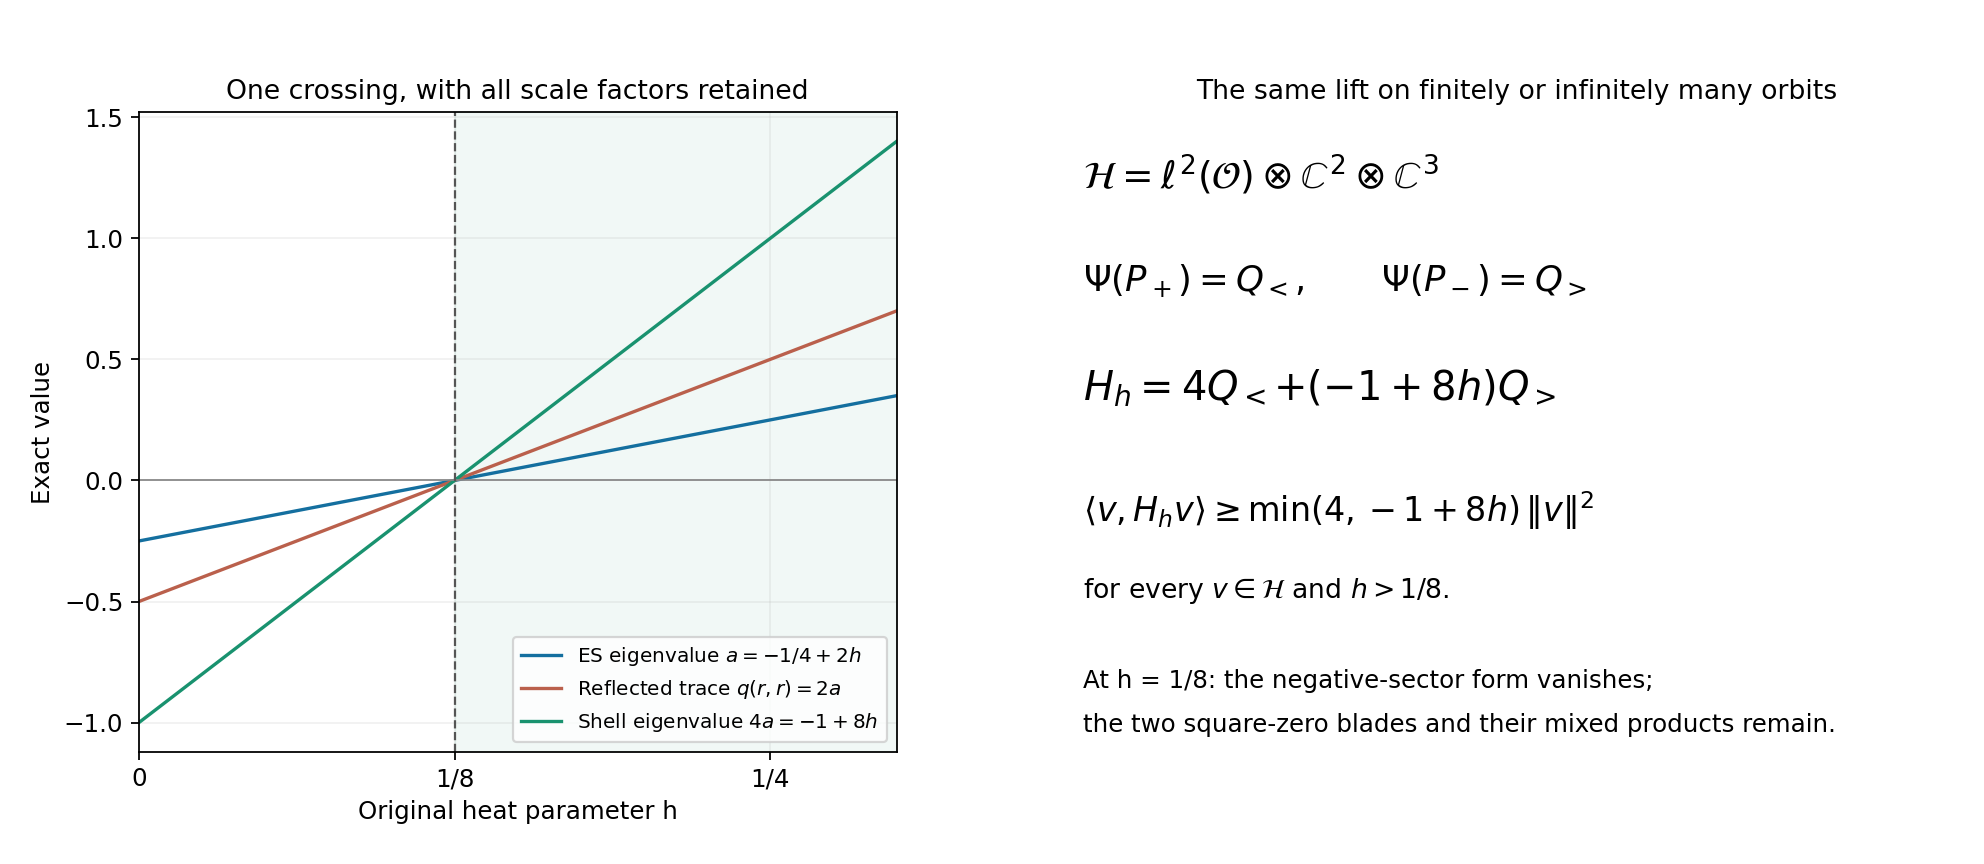
\includegraphics[keepaspectratio,alt={The three exact changing coefficients and their common crossing. The quarter coefficient is a, its reflected trace is 2a, and the shell coefficient is 4a. ESHL12--ESHL25 and ESHL34--ESHL42 prove the finite and infinite maps, sharp bound, surviving blades and trace scope.}]{figures/28_shell_heat_sign.png}}
\caption{The three exact changing coefficients and their common
crossing. The quarter coefficient is a, its reflected trace is 2a, and
the shell coefficient is 4a. ESHL12--ESHL25 and ESHL34--ESHL42 prove the
finite and infinite maps, sharp bound, surviving blades and trace
scope.}
\end{figure}

\clearpage

\section{The actual Weil correction has the ES three-plus-one
form}\label{the-actual-weil-correction-has-the-es-three-plus-one-form}

This calculation identifies the finite correction in the full explicit
formula with the original ES quarter form. It uses actual compactly
supported smooth tests, proves a section onto all four evaluation
coordinates, and retains the kernel. It does not identify this finite
correction with the entire Weil pairing. The needed endpoint conventions
and completion identity are proved in
\href{https://github.com/KokunoYumeto/zeta-function-research-reader/blob/d5c9d198a8432e3ede468b280162a99c00e3f4f7/workbenches/splitzero-tandem/branches/tau-zero-prime-positivity/HEAT_ENDPOINT_SIGN_BRIDGE.md}{the
complete heat endpoint sign bridge proof}, HEB11--HEB17 and
HEB23--HEB36; the exact original ES metric and its isometry are proved
in
\href{https://github.com/KokunoYumeto/zeta-function-research-reader/blob/d5c9d198a8432e3ede468b280162a99c00e3f4f7/workbenches/splitzero-tandem/branches/tau-zero-prime-positivity/ES_QUARTER_HEAT_TRACE_DERIVATION.md}{the
complete es quarter heat trace derivation proof}, ESQ9--ESQ27. Every
comparison needed here is calculated below.

\subsection{1. Four evaluation coordinates of an admissible
test}\label{four-evaluation-coordinates-of-an-admissible-test}

Let \(\mathcal T=C_c^\infty(\mathbb R;\mathbb C)\) and retain \[
M_f(s)=\int_{\mathbb R}f(v)e^{-(s-1/2)v}\,dv,
\quad (s_1,s_2,s_3,s_4)=(0,1,1/2+i/2,1/2-i/2).
\tag{WEC1}
\] Set \(t_j=s_j-1/2\), \(k_j(v)=e^{-t_jv}\), and define \[
L:\mathcal T\longrightarrow\mathbb C^4,
\qquad Lf=(A,B,C,D)=(M_f(s_1),M_f(s_2),M_f(s_3),M_f(s_4)).
\tag{WEC2}
\] The integral defines an entire function of \(s\), since its
derivatives converge uniformly on each compact set and the support in
\(v\) is compact.

Here is a concrete linear section for every four-tuple. Choose the
normalized positive even smooth bump \(\psi\) on \((-1,1)\) in HEB33 and
put \[
G_{ij}=\int_{\mathbb R}\psi(v)k_i(v)\overline{k_j(v)}\,dv,
\qquad
S(y)(v)=\psi(v)\sum_{j=1}^4(G^{-1}y)_j\overline{k_j(v)}.
\tag{WEC3}
\] The matrix \(G\) is positive definite. Indeed, for
\(z\in\mathbb C^4\),
\(z^*Gz=\int\psi(v)|\sum_i\overline z_i k_i(v)|^2\,dv\). If this equals
zero, the continuous sum vanishes on \((-1,1)\), where \(\psi>0\). Its
derivatives of orders \(0,1,2,3\) at zero give
\(\sum_i\overline z_i(-t_i)^m=0\). The four numbers \(-t_i\) are
distinct, so this Vandermonde matrix is invertible: its determinant is
\(\prod_{i<j}((-t_j)-(-t_i))\ne0\), obtained by the usual polynomial
alternating-factor expansion (both sides have the same degree and
leading coefficient). Thus \(z=0\). This proves positive definiteness
and existence of the displayed inverse.

The section \(S(y)\) is smooth and compactly supported because it is a
finite sum of smooth exponentials times \(\psi\). Direct integration
gives \[
L S(y)=GG^{-1}y=y.
\tag{WEC4}
\] Consequently \(L\) is onto, and
\(\mathcal T=\ker L\oplus S(\mathbb C^4)\) as complex vector spaces,
with projection \(SL\). This proves that no hidden condition on
admissible tests prevents the four coordinates used below.

\subsection{2. The exact endpoint gain and its full-form
compensation}\label{the-exact-endpoint-gain-and-its-full-form-compensation}

At heat time \(h=1/4\), the moving endpoint polynomial is
\(s(s-1)+1/2\), whose roots are \(s_3,s_4\). The two forms on actual
tests are therefore \[
\begin{aligned}
P_0(f,g)&=\overline{A_f}B_g+\overline{B_f}A_g,\\
P_{1/4}(f,g)&=\overline{C_f}C_g+\overline{D_f}D_g.
\end{aligned}
\tag{WEC5}
\] This follows from the endpoint involution \(s^\#=1-s\) together with
coefficient conjugation: it exchanges \(0,1\) and fixes each
critical-line point in the reflected evaluation. Define the finite gain
form \[
\mathcal C=P_{1/4}-P_0.
\tag{WEC6}
\] In the actual four values its quadratic expression is \[
\mathcal C(f,f)=|C|^2+|D|^2+\frac{1}{2}|A-B|^2-\frac{1}{2}|A+B|^2.
\tag{WEC7}
\] Expansion of the last two squares gives
\(-\overline A B-\overline B A\), proving the formula. In coordinates
\((C,D,(A-B)/\sqrt2,(A+B)/\sqrt2)\), its matrix is
\(\operatorname{diag}(1,1,1,-1)\). Hence its quotient has signature
\((3,1)\). More precisely its radical on \(\mathcal T\) is exactly
\(\ker L\): the inclusion follows from (WEC5), while if \(Lf\ne0\),
nondegeneracy of this displayed matrix supplies a vector \(y\) with
nonzero pairing against \(Lf\), and the admissible test \(S(y)\) detects
it by (WEC4).

Let \(\mathcal A\) and \(\mathcal P\) denote the original archimedean
and rational-prime terms. The full Weil form remains \[
W=P_0+\mathcal A-\mathcal P
=P_{1/4}+(\mathcal A-\mathcal C)-\mathcal P.
\tag{WEC8}
\] This is the exact completion correction, not a discarded residual:
logarithmic differentiation of \(\Lambda_{1/4}=2\xi/[s(s-1)+1/2]\) adds
\(q_0'/q_0-q_{1/4}'/q_{1/4}\), and the residues at the four simple roots
yield \(P_0-P_{1/4}=-\mathcal C\). Thus the correction subtracted from
the archimedean term is the same nondegenerate \((3,1)\) quotient just
computed; its negative has signature \((1,3)\).

\subsection{3. An explicit isometry to the original ES quarter
form}\label{an-explicit-isometry-to-the-original-es-quarter-form}

Retain the original raw ordering \((E_{11},E_{12},E_{21},E_{22})\) and
the forced ES metric and initial quarter operator \[
G_{\rm ES}=\begin{pmatrix}
1/16&0&0&-7/144\\0&2/9&0&0\\0&0&1&0\\-7/144&0&0&1/16
\end{pmatrix},\qquad
A_0=\operatorname{diag}(1/4,1/4,-1/4,1/4).
\tag{WEC9}
\] They are the original source matrices used in ESQ9 and ESQ2. Define
the linear map \(J:\mathbb C^4\to M_2(\mathbb C)\) by \[
\begin{aligned}
x_{11}&=12C+3\sqrt2D,&x_{22}&=12C-3\sqrt2D,\\
x_{12}&=3(A-B),&x_{21}&=\sqrt2(A+B).
\end{aligned}
\tag{WEC10}
\] It is invertible, with \[
C=\frac{x_{11}+x_{22}}{24},\quad D=\frac{x_{11}-x_{22}}{6\sqrt2},\quad
A=\frac12\left(\frac{x_{21}}{\sqrt2}+\frac{x_{12}}3\right),\quad
B=\frac12\left(\frac{x_{21}}{\sqrt2}-\frac{x_{12}}3\right).
\tag{WEC11}
\] Substitution in both orders gives each of the four starting
coordinates. From the displayed matrix multiplication, \[
x^*G_{\rm ES}A_0x=
\left|\frac{x_{11}+x_{22}}{24}\right|^2+
\left|\frac{x_{11}-x_{22}}{6\sqrt2}\right|^2+
\frac{|x_{12}|^2}{18}-\frac{|x_{21}|^2}{4}.
\tag{WEC12}
\] For example the first two squares expand to
\((|x_{11}|^2+|x_{22}|^2)/64-(7/288)\operatorname{Re}(\overline{x_{11}}x_{22})\),
exactly the two diagonal entries and mixed term of \(G_{\rm ES}A_0\).
Substituting (WEC10) in (WEC12) gives (WEC7). Polarization, or the same
expansion in two slots, therefore proves the isometry \[
\boxed{\mathcal C(f,g)=(JLf)^*G_{\rm ES}A_0(JLg).}
\tag{WEC13}
\] The map \(JL\) is onto, has kernel \(\ker L\), and has explicit
section \(SJ^{-1}\). This proves an isomorphism of the nondegenerate
Hermitian quotient \(\mathcal T/\ker L\) with the actual complexified ES
quarter form, including its coordinates, constants and sign. It is a
linear form isomorphism, not an asserted ring isomorphism of a
test-function multiplication with raw matrix multiplication.

The form identity links the tetrahedral description to an actual term of
the Weil formula: it is the finite endpoint-change correction. It does
not identify the remaining \(\mathcal A-\mathcal P\), or the full form
\(W\), with this four-dimensional quotient. Equation (WEC8) records
exactly where that quotient enters.

\subsection{4. Actual positive and negative gain
tests}\label{actual-positive-and-negative-gain-tests}

The section (WEC3) supplies explicit admissible tests for both signs.
For \[
f_-=S(1,1,0,0),\qquad f_+=S(1,-1,0,0),
\tag{WEC14}
\] one has \(P_{1/4}(f_\pm,f_\pm)=0\), while \(P_0(f_-,f_-)=2\) and
\(P_0(f_+,f_+)=-2\). Thus \(\mathcal C(f_-,f_-)=-2\) and
\(\mathcal C(f_+,f_+)=2\). These are tests of the endpoint gain; they do
not give negative values of the full classical Weil form. The bump
derivative in HEB33--HEB36 supplies a single test whose endpoint term
passes from negative, through a nonzero nilpotent with zero pairing, to
positive, with the exact opposite change in the archimedean term.

\subsection{5. The actual test involution and its exact ES
intertwiner}\label{the-actual-test-involution-and-its-exact-es-intertwiner}

The involution on tests is \(f^\#(v)=\overline{f(-v)}\). Changing
variables in (WEC1) gives \(M_{f^\#}(s)=\overline{M_f(1-\overline s)}\),
so its action on the four coordinates is \[
(A,B,C,D)^\#=(\overline B,\overline A,\overline C,\overline D).
\tag{WEC15}
\] Under the map \(J\) in (WEC10), the transported action on raw
coordinates is \(T_0x=\operatorname{diag}(1,-1,1,1)\overline x\): only
\(A-B\) changes sign. The original ES anti-linear quarter involution is
instead
\(T_{\rm ES}x=(4A_0)\overline x=\operatorname{diag}(1,1,-1,1)\overline x\).
Their exact comparison is \[
T_{\rm ES}=C_0T_0,\qquad C_0=\operatorname{diag}(1,-1,-1,1).
\tag{WEC16}
\] On raw matrices \(C_0\) is conjugation by
\(\operatorname{diag}(1,-1)\), as direct multiplication shows. Both
involutions and their relation are thereby retained.

There is also an isometry that intertwines the two anti-linear actions.
Put \[
U=\operatorname{diag}(1,i,i,1),\qquad\widehat J=UJ.
\tag{WEC17}
\] The only off-diagonal entries of \(G_{\rm ES}A_0\) connect the first
and fourth positions, on which \(U\) is the identity. On the other two
positions multiplication by \(i\) preserves the absolute squares. Hence
\(U^*(G_{\rm ES}A_0)U=G_{\rm ES}A_0\). For the anti-linear comparison
the matrix is
\(U\operatorname{diag}(1,-1,1,1)\overline{U^{-1}}=\operatorname{diag}(1,1,-1,1)\),
by multiplication of its four diagonal entries. Consequently \[
\mathcal C(f,g)=(\widehat JLf)^*G_{\rm ES}A_0(\widehat JLg),
\qquad \widehat JL(f^\#)=T_{\rm ES}\widehat JL(f).
\tag{WEC18}
\] The inverse and section are \(J^{-1}U^{-1}\) and \(SJ^{-1}U^{-1}\).
Explicitly \(\widehat J\) changes just two entries of (WEC10) to
\(x_{12}=3i(A-B)\), \(x_{21}=i\sqrt2(A+B)\). Thus both the Hermitian
form and the specified involution are preserved by a proved map. The map
\(U\) is not a raw-matrix algebra automorphism: it fixes \(E_{11}\),
while \(U(E_{12})U(E_{21})=-E_{11}\). No multiplication compatibility
beyond its stated linear and involution properties is assumed.

\begin{figure}
\centering
\pandocbounded{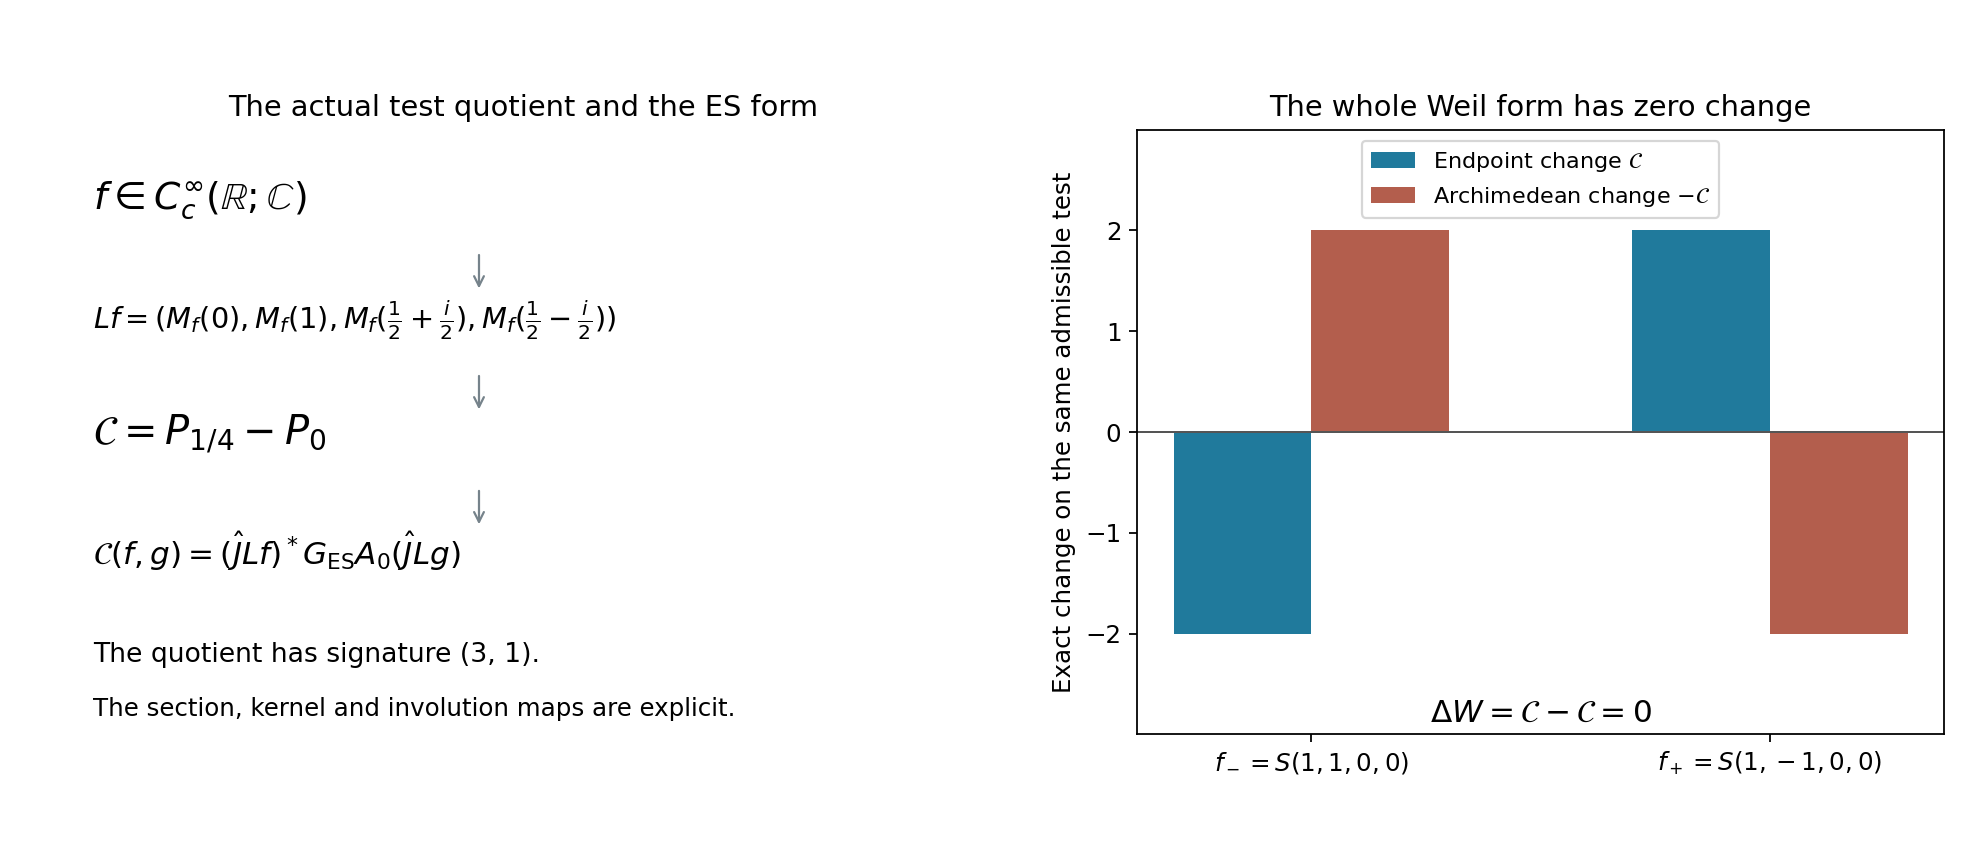
\includegraphics[keepaspectratio,alt={The actual four-value correction, its exact ES isometry, and its cancellation in the full Weil form. WEC1--WEC18 give all maps, the section and the two admissible tests.}]{figures/29_actual_weil_correction.png}}
\caption{The actual four-value correction, its exact ES isometry, and
its cancellation in the full Weil form. WEC1--WEC18 give all maps, the
section and the two admissible tests.}
\end{figure}

\clearpage

\section{The signed eight-state completion and its exact heat
receivers}\label{the-signed-eight-state-completion-and-its-exact-heat-receivers}

This note compares the original seven-point affine chart with its
eight-state signed completion, keeping both original involutions. It
calculates the complete trace forms, identifies the missing infinity
state, and constructs a target path whose marked-root quotient is
exactly the HEB heat family. The whole eight-state form is calculated on
that path, including its length-four collision algebra.

The original sources actually read are
\href{https://github.com/KokunoYumeto/zeta-function-research-reader/blob/ab45e221579a0d48ce2885b4ecdf1a6aefc24a20/workbenches/splitzero-tandem/continuations/20260920-fable-boundary-action/FABLE_TO_ORIGINAL_CONDUCTOR.tex}{\emph{The
ES--Fable inverse correspondence in the original weighted conductor},
FC36--FC47}, and
\href{https://github.com/KokunoYumeto/zeta-function-research-reader/blob/0fd693c844aad9117e30ec447c59864a28af10f3/workbenches/splitzero-tandem/continuations/20260921-native-spectral-real-pair/005/independent/FINITE_SIGNED_COMPLETION.tex}{\emph{The
finite signed-root completion with all original fibre algebras},
FS1--FS27 and FS30--FS31}. The latter pinned TeX has the same bytes as
the local source used here. Its reciprocal-coordinate construction,
chart transitions, trace and local algebra proofs are retained. The
receiving HEB equations are HEB15--HEB20 and HEB31--HEB32 of
\href{https://github.com/KokunoYumeto/zeta-function-research-reader/blob/d5c9d198a8432e3ede468b280162a99c00e3f4f7/workbenches/splitzero-tandem/branches/tau-zero-prime-positivity/HEAT_ENDPOINT_SIGN_BRIDGE.md}{the
complete heat endpoint sign bridge proof}, read in full during the
quarter comparison. The original heat clock also has the public proof
\href{https://github.com/KokunoYumeto/zeta-function-research-reader/blob/ac168d55cbb400a6c8926a00d67909ba65646ac5/satellites/26_incompressible_fibre_heat.tex\#L389}{\emph{The
original heat trajectories}, \texttt{eq:\allowbreak{}ifh-\allowbreak{}target-\allowbreak{}flow}}. All new
comparisons and their hypotheses are proved below.

\subsection{1. The original coordinates and the two completion
charts}\label{the-original-coordinates-and-the-two-completion-charts}

Write the first source coordinate called \(a\) in FS1 as \(\alpha\),
solely to distinguish it from the HEB coefficient \(a_H\). This is the
identity renaming of that coordinate. The other source coordinates
remain \((y,z,w)\). The original factors are \[
\begin{aligned}
b&=i+\alpha y,&c&=-i+2\alpha y+\alpha^2z,\\
d&=-iy-\alpha(iz+2y^2)-\alpha^2yz,&
e&=2z-7iy^2+\alpha w,\\
f&=iw+3iy^3-4yz+\alpha(6iy^2z+wy+4y^4)+2\alpha^2y^3z.
\end{aligned}
\tag{ESH1}
\] The target is \(\mathbf U=(A,B,C,D)\), where \[
P=(\alpha c,\alpha e+bd,\alpha f+be,bf),\qquad
H_{\mathbf U}(U,V)=AU^4+U^3V+BU^2V^2+CUV^3+DV^4.
\tag{ESH2}
\] The retained factor identities are \(\alpha d+bc=1\) and
\(\alpha^3f-\alpha^2be+\alpha b^2d-b^3c=1\). They follow by substituting
(ESH1), and are the exact identities proved in FS1 and FC44--FC44b. Thus
\((\alpha U+bV)(cU^3+dU^2V+eUV^2+fV^3)=H_{\mathbf U}\), with resultant
one. The cubic coefficient is fixed at one; it is not another free
parameter.

Use \(R\) for the finite marked root called \(r\) in FS2, and \(T\) for
its reciprocal factor called \(t\). The finite completed chart and the
infinity chart are \[
F_{\mathbf U}(R)=AR^4+R^3+BR^2+CR+D,
\qquad F_{\mathbf U}(R)=0,\quad T^2=F'_{\mathbf U}(R),
\tag{ESH3}
\] \[
k_{\mathbf U}(v)=A+v+Bv^2+Cv^3+Dv^4,
\qquad k_{\mathbf U}(v)=0,\quad \Theta^2=-k'_{\mathbf U}(v).
\tag{ESH4}
\] On their overlap the maps are \[
v=R^{-1},\quad \Theta=-T/R,\qquad
R=v^{-1},\quad T=-\Theta/v.
\tag{ESH5}
\] They are inverse by substitution. Differentiating \(k(v)=v^4F(1/v)\)
at a root gives \(k'(v)=-v^2F'(1/v)\), which verifies the
squared-coordinate relation and its sign. On the original finite factor
chart, \[
R=-b/\alpha=-y-i/\alpha,\qquad T=1/\alpha,
\qquad \alpha^2F'_{\mathbf U}(R)=1.
\tag{ESH6}
\] The finite completion allows \(T=0\); it does not declare
\(1/\alpha\) to be an invertible coordinate at that boundary.

For reference, the inverse factor formulas on \(T\ne0\) are \[
\begin{aligned}
\alpha&=T^{-1},&b&=-R/T,&c&=AT,\\
d&=(1+AR)T,&e&=(B+R+AR^2)T,&
f&=(C+BR+R^2+AR^3)T.
\end{aligned}
\tag{ESH7}
\] They give \(\alpha d+bc=1\) directly. Their four product coefficients
are \(A,B,C\), and \(-R(C+BR+R^2+AR^3)=D\), the last by \(F(R)=0\).
Their resultant is \(T^{-2}F'(R)=1\). Thus these formulas prove the
factor reconstruction with its original reciprocal coordinate.

At \(v=0\), the infinity equations give \[
A=0,\qquad \Theta^2=-1,\qquad
\Theta=-i\text{ is included},\quad \Theta=i\text{ is omitted}.
\tag{ESH8}
\] Indeed the infinity factor chart has \(b=\Theta^{-1}\); the original
source at \(\alpha=0\) has \(b=i\) by (ESH1), so its value is
\(\Theta=-i\). The other sign has \(b=-i\) and does not belong to that
original chart. This is the precise meaning of the missing eighth state.

The missing infinity point is unramified. The relative derivative matrix
of (ESH4) with respect to \((v,\Theta)\) has determinant
\(2\Theta k'(v)\); at \(v=0\) its value is \(2\Theta\ne0\), since
\(k'(0)=1\). This matrix is invertible there, proving the vanishing of
the relative differential module and the absence of ramification in that
chart. On the finite chart the same determinant is \(2T F'(R)=2T^3\), so
its ramification support is \(T=0\). The infinity points never belong to
that support. These calculations reproduce the relevant part of
FS16--FS17 and prove that the omitted infinity sign is not the nilpotent
collision.

\subsection{2. The entire completed fibre at the original seven-point
target}\label{the-entire-completed-fibre-at-the-original-seven-point-target}

At \[
\mathbf U_*=(0,0,-1,0),\qquad
H_*(U,V)=UV(U-V)(U+V),\qquad F_*(R)=R^3-R,
\tag{ESH9}
\] the projective roots are \(\infty,0,1,-1\), all simple. At the finite
roots the derivative values are \[
F'_*(0)=-1,\qquad F'_*(1)=F'_*(-1)=2.
\tag{ESH10}
\] The completed complex fibre algebra is therefore exactly \[
\mathcal A_*=
\frac{\mathbb C[T_0]}{(T_0^2+1)}
\times\frac{\mathbb C[T_+]}{(T_+^2-2)}
\times\frac{\mathbb C[T_-]}{(T_-^2-2)}
\times\frac{\mathbb C[\Theta]}{(\Theta^2+1)}.
\tag{ESH11}
\] To prove the finite splitting, the idempotents in
\(\mathbb C[R]/(R^3-R)\) are \[
e_0=1-R^2,\qquad e_+=(R^2+R)/2,\qquad e_-=(R^2-R)/2.
\tag{ESH12}
\] They evaluate as the three separate indicator functions at
\(0,1,-1\). Their products, sum and squares are consequently the
orthogonal idempotent identities: a polynomial remainder of degree at
most two vanishing at the three distinct roots is zero. Applying those
idempotents to the relation \(T^2=3R^2-1\) gives the first three factors
in (ESH11). The infinity root is the disjoint fourth root of the
projective root fibre, and (ESH8) gives its fourth factor. Each
quadratic has two distinct roots, so each is reduced and of dimension
two. The total dimension is eight and every geometric point is reduced.

The eight points are \[
(0,\pm i),\quad(1,\pm\sqrt2),\quad(-1,\pm\sqrt2),
\quad(\infty,\Theta=\pm i).
\tag{ESH13}
\] The first entry marks the projective root; the second is its retained
sign coordinate. The source chart includes the first six and
\((\infty,-i)\). At the latter, FS13 gives the original point
\((\alpha,y,z,w)=(0,0,i/2,0)\). At \((\infty,i)\), the factor
coordinates are exactly \[
(\alpha,b,c,d,e,f)=(0,-i,i,0,-i,0),
\tag{ESH14}
\] by (ESH8) and the product coefficients. This is the omitted sign in
FC44b, not an additional root or an identification of two labels.

\subsection{3. Both original involutions, with coefficient conjugation
separate}\label{both-original-involutions-with-coefficient-conjugation-separate}

The completed sign deck involution is \[
\Sigma:(R,T)\longmapsto(R,-T),\qquad
(v,\Theta)\longmapsto(v,-\Theta).
\tag{ESH15}
\] Its formulas agree through (ESH5), preserve the equations, and square
to the identity. They are the completed version of the simultaneous
factor sign in FC43--FC44. Let \(\kappa\) conjugate coefficients and fix
the displayed coordinate generators; it is defined on a fibre over real
\((A,B,C,D)\). The conjugate-deck involution is
\(\#_\Sigma=\Sigma\kappa\), so it negates \(T,\Theta\) and fixes the
real root variable \(R\), while conjugating scalars.

The other original involution is \[
J(\alpha,y,z,w)=(-\alpha,-y,z,-w).
\tag{ESH16}
\] Substituting in (ESH1) sends the factor tuple to
\(( -\alpha,b,c,-d,e,-f)\), so its target map and completion charts are
\[
J_{\mathrm{out}}(A,B,C,D)=(-A,-B,C,-D),
\tag{ESH17}
\] \[
J:(R,T)\longmapsto(-R,-T),\qquad
(v,\Theta)\longmapsto(-v,\Theta).
\tag{ESH18}
\] The first formula follows from (ESH6), and the second from (ESH5). To
verify the equations on their whole domains, one has
\(F_{J_{\mathrm{out}}\mathbf U}(-R)=-F_{\mathbf U}(R)\),
\(F'_{J_{\mathrm{out}}\mathbf U}(-R)=F'_{\mathbf U}(R)\), and the
identical two identities for \(k\) at \(-v\). Thus (ESH18) is the full
map, including completion points. The target \(\mathbf U_*\) is fixed,
so \(\#_J=J\kappa\) is an involution of this fibre. It is different from
\(\#_\Sigma\).

\subsection{4. The complete trace forms and their
signatures}\label{the-complete-trace-forms-and-their-signatures}

For the quadratic algebra \(K_\mu=\mathbb C[T]/(T^2-\mu)\), with real
\(\mu\ne0\), multiplication in the unchanged basis \((1,T)\) gives \[
\operatorname{Tr}_{K_\mu}(c+dT)=2c.
\tag{ESH19}
\] Indeed multiplication by \(T\) has matrix
\(\begin{psmallmatrix}0&\mu\\1&0\end{psmallmatrix}\). Hence the
coefficient-conjugation and conjugate-deck Hermitian forms have
respective Gram matrices \[
[Q_\kappa]=\operatorname{diag}(2,2\mu),\qquad
[Q_{\#_\Sigma}]=\operatorname{diag}(2,-2\mu),
\quad Q_\iota(x,y)=\operatorname{Tr}(\iota(x)y).
\tag{ESH20}
\] These formulas follow also by multiplying \((\bar c+\bar dT)(e+fT)\)
or \((\bar c-\bar dT)(e+fT)\) and taking twice the scalar coefficient.
They verify the full forms in both arguments.

In the factor order of (ESH11), with each basis \((1,T)\) retained, the
whole Gram matrices are \[
[Q_\kappa]=\operatorname{diag}(2,-2,2,4,2,4,2,-2),
\tag{ESH21}
\] \[
[Q_{\#_\Sigma}]=\operatorname{diag}(2,2,2,-4,2,-4,2,2).
\tag{ESH22}
\] Both happen to have inertia \((6,2,0)\), but their negative subspaces
belong to different factors. Here and below inertia lists positive,
negative and radical dimensions. The complex bilinear trace without an
antilinear involution has no ordered signature; (ESH21) is its
coefficient-conjugation Hermitian version, or its real coefficient
restriction.

The native involution has a different complete matrix. In the ordered
basis \[
(e_0,e_0T,\ e_+,e_-,\ e_+T,e_-T,\ e_\infty,e_\infty\Theta)
\] one has \[
[Q_{\#_J}]=
\begin{pmatrix}2&0\\0&2\end{pmatrix}
\oplus\begin{pmatrix}0&2\\2&0\end{pmatrix}
\oplus\begin{pmatrix}0&-4\\-4&0\end{pmatrix}
\oplus\begin{pmatrix}2&0\\0&-2\end{pmatrix}.
\tag{ESH23}
\] For proof, (ESH18) fixes the root 0 and negates its sign,
interchanges \(e_+,e_-\) and negates \(T\), and fixes the infinity
coordinate \(\Theta\). Thus, for example, \(\#_J(e_+T)=-e_-T\), whose
pairing with \(e_-T\) is \(-\operatorname{Tr}(2e_-)=-4\). The mixed
products between different root factors vanish, and (ESH20) gives the
remaining blocks. Each off-diagonal two-by-two block has one eigenvalue
of each sign. Therefore \[
\operatorname{inertia}(Q_{\#_J})=(5,3,0).
\tag{ESH24}
\] Neither calculation assumes that one of these finite forms is the
global Weil form.

\subsection{5. Omitting precisely one of the eight
states}\label{omitting-precisely-one-of-the-eight-states}

Let \(m=(\infty,i)\) be the missing point. Its idempotent, supported in
the infinity factor, is \[
e_m=(0,0,0,(1-i\Theta)/2),\qquad
e_n=(0,0,0,(1+i\Theta)/2),
\tag{ESH25}
\] where \(n=(\infty,-i)\) is the retained point. Evaluation at
\(\Theta=\pm i\) verifies that these are the respective indicator
functions. Therefore the exact original seven-state quotient is \[
q:\mathcal A_*\longrightarrow\mathcal A_7:=\mathcal A_*/\mathbb Ce_m,
\qquad
\mathcal A_*\cong\mathcal A_7\times\mathbb C.
\tag{ESH26}
\] The last factor is evaluation at \(m\). Its inverse inserts that
value at the omitted coordinate, while the canonical nonunital section
of \(q\) inserts zero there. These maps are the full coordinate maps,
not a count alone.

Coefficient conjugation in (ESH25) gives the exact stability results \[
\#_\Sigma(e_m)=e_m,\qquad
\Sigma(e_m)=\kappa(e_m)=e_n,
\qquad J(e_m)=e_m,\quad \#_J(e_m)=e_n.
\tag{ESH27}
\] Thus \(\#_\Sigma\) descends to \(\mathcal A_7\), whereas \(\Sigma\),
\(\kappa\), and \(\#_J\) individually do not. Pure native \(J\) does
descend. For the descended conjugate-deck trace one has, on arbitrary
lifts \(f,g\), \[
Q_{\#_\Sigma,7}(qf,qg)
=Q_{\#_\Sigma,*}(f,g)-\overline{f(m)}g(m).
\tag{ESH28}
\] This follows from the direct-product trace and the fact that \(m\) is
fixed by the point action of \(\#_\Sigma\). The removed summand is
positive. Consequently \[
\operatorname{inertia}(Q_{\#_\Sigma,7})=(5,2,0).
\tag{ESH29}
\] In particular the two explicit retained vectors \(e_+T,e_-T\) still
have value \(-4\), and are mutually orthogonal by (ESH22). Removing the
omitted infinity point has not removed either negative direction.

For the native Hermitian form there is instead the restriction to the
retained corner \((1-e_m)\mathcal A_*\). Its infinity line
\(\mathbb Ce_n\) is radical because \(\#_J(e_n)=e_m\), whose product
with every retained element is zero. The other six-dimensional block has
inertia \((4,2,0)\) from (ESH23), so this restricted form has \[
\operatorname{inertia}
\bigl(Q_{\#_J}|_{(1-e_m)\mathcal A_*}\bigr)=(4,2,1).
\tag{ESH30}
\] It is not a trace form of a descended native involution. Indeed
\(Q_{\#_J}(e_m,e_n)=\operatorname{Tr}(e_n)=1\), so adding a
representative from the killed ideal can change the original pairing.
This proves directly why that full form cannot be defined on the
quotient by choosing arbitrary lifts.

The exact native-stable quotient generated by this omission is also
determined. The smallest \(\#_J\)-stable ideal containing
\(\mathbb Ce_m\) is \[
\mathcal I_{\mathrm{stable}}=\mathbb Ce_m\oplus\mathbb Ce_n
=e_\infty\mathcal A_*.
\tag{ESH30a}
\] Every stable ideal containing \(e_m\) must contain its image \(e_n\);
conversely their sum is an ideal and is stable by (ESH27). This proves
minimality and the universal quotient property: any algebra quotient
with an induced native involution and killing \(e_m\) factors uniquely
through \(\mathcal A_6=\mathcal A_*/\mathcal I_{\mathrm{stable}}\), the
product of the three finite root factors. Its native trace form has
inertia \((4,2,0)\) by the first three blocks of (ESH23). The restricted
seven-dimensional form (ESH30) factors through the further projection
\(\mathcal A_7\to\mathcal A_6\), whose kernel is its radical
\(\mathbb Ce_n\). This gives the complete projection and radical maps,
rather than an involution assigned to a nonstable quotient.

Restoring the eighth coordinate has a different exact effect. In the
infinity point basis \((e_m,e_n)\), the native trace block is \[
\begin{pmatrix}0&1\\1&0\end{pmatrix}.
\tag{ESH30b}
\] The diagonal entries vanish because the two different point
idempotents multiply to zero after applying \(\#_J\), and the cross
entries are the trace-one values just computed. Its eigenvectors
\(e_m+e_n\) and \(e_m-e_n\) have positive and negative values 2 and
\(-2\). Completing the eighth state therefore restores the full
nondegenerate hyperbolic pair, whose restriction to the retained
one-dimensional infinity corner was radical. Under \(\#_\Sigma\), by
contrast, these two point idempotents are separately fixed and form two
positive scalar summands, as (ESH27)--(ESH29) show.

There is a literal occurrence of the fraction \(1/8\) in the normalized
trace, with a different meaning. If
\(\operatorname{tr}_8=\operatorname{Tr}/8\), then \[
\operatorname{tr}_8(1)=1,\qquad
\operatorname{tr}_8(e_m)=1/8,\qquad
\operatorname{tr}_8(e_\infty)=1/4.
\tag{ESH31}
\] These follow because the three idempotents have ranks eight, one and
two as multiplication projectors. The value \(1/8\) is the normalized
mass of that one reduced state. It supplies no parameter evolution by
itself. The next sections give actual parameter maps and calculate their
full forms.

\subsection{6. Exact boundary maps to the HEB quadratic
forms}\label{exact-boundary-maps-to-the-heb-quadratic-forms}

Write the HEB algebra and involution as \[
E_{a_H}=\mathbb C[r_H]/(r_H^2+a_H),\qquad
r_H^\#=-r_H,\quad z^\#=\bar z\ (z\in\mathbb C).
\tag{ESH32}
\] Its full regular trace form in basis \((1,r_H)\) is
\(\operatorname{diag}(2,2a_H)\), by the same multiplication argument as
(ESH19)--(ESH20). The original heat clock is \(a_H(h)=-1/4+2h\).

For the infinity algebra \(I=\mathbb C[\Theta]/(\Theta^2+1)\), the exact
conjugate-deck isomorphism is \[
\phi_\Sigma:E_{1/4}\xrightarrow{\sim}I,
\qquad r_H\longmapsto\Theta/2,
\qquad\phi_\Sigma^{-1}(\Theta)=2r_H.
\tag{ESH33}
\] The squared relation follows from \(\Theta^2=-1\), and substitution
gives both inverse compositions. Since \(\#_\Sigma(\Theta)=-\Theta\),
the map preserves the involution. An algebra isomorphism conjugates
multiplication matrices in the corresponding bases, so preserves regular
trace and hence the full reflected pairing. Equivalently the target
matrix \(\operatorname{diag}(2,2)\) pulls back under \(r_H=\Theta/2\) to
\(\operatorname{diag}(2,1/2)\), exactly the HEB matrix at \(a_H=1/4\).
That value corresponds to heat time \(h=1/4\), not the nilpotent time
\(h=1/8\).

For the native involution on the same infinity algebra there is a
different exact comparison: \[
\phi_J:E_{-1/4}\xrightarrow{\sim}I,
\qquad r_H\longmapsto i\Theta/2,
\qquad\phi_J^{-1}(\Theta)=-2i r_H.
\tag{ESH34}
\] Here \((i\Theta/2)^2=1/4\), so the source relation is respected.
Native \(\#_J\) fixes \(\Theta\) and conjugates \(i\), hence negates
\(i\Theta/2\). Both inverse compositions and involution compatibility
follow by substitution, and the algebra isomorphism again preserves
trace. Its form has inertia \((1,1,0)\), corresponding to HEB heat time
\(h=0\). The scalar \(i\) is part of the map: this is a complex algebra
and conjugate-linear-involution comparison, not an identification of the
coefficient-fixed real presentations. In particular (ESH33) must not be
used as a native-involution isometry.

The factor projection \(\mathcal A_*\to I\) and the corner inclusion
\(I\to\mathcal A_*\), with zero in the three other factors, are explicit
algebra maps. The projection is unital; the inclusion sends its unit to
\(e_\infty\). The inclusion preserves regular trace and the
corresponding involution, while the projection retains only its factor
contribution to the total trace. No unital trace-preserving map from the
entire rank-eight algebra to this rank-two algebra could exist, since
the traces of their units are eight and two. The full trace comparison
is the sum of the four factor traces in (ESH11), not the projection
alone.

The reduced infinity pair is not the collision algebra \(E_0\), and
their precise morphisms show what is lost. Every unital complex algebra
map \(I\simeq\mathbb C^2\to E_0\) is one of the two point evaluations
followed by the scalar inclusion. Indeed an idempotent in \(E_0\) has
form \(c+dr_H\); its square equation gives \(c^2=c\) and \((2c-1)d=0\),
hence it is 0 or 1. The two complementary idempotents of \(I\) must
therefore map to 0 and 1. Conversely each choice is a map. Every unital
map \(E_0\to I\) kills \(r_H\), since its image would be nilpotent in
the reduced algebra \(I\); hence it is the reduction map followed by the
diagonal scalar inclusion. Thus every composite from \(E_0\) through
\(I\) kills its nonzero nilpotent. The retained dual-number direction is
genuinely present in the other heat receiver constructed next.

\subsection{7. A target path whose marked-root quotient is exactly the
original heat
algebra}\label{a-target-path-whose-marked-root-quotient-is-exactly-the-original-heat-algebra}

Define the following explicit path in the unchanged quartic coefficient
target: \[
\gamma_+(h)=(0,0,-1-16h,16h),\qquad
F_h(R)=R^3-(1+16h)R+16h
=(R-1)(R^2+R-16h).
\tag{ESH35}
\] It begins at \(\mathbf U_*\). This is a target path chosen to pull
back the HEB clock; it is not asserted to be a native PDE evolution of
the whole quartic. The marked root \(R=1\) is retained for every
parameter, and \[
F'_h(1)=2-16h=-8a_H(h).
\tag{ESH36}
\] The finite signed algebra over this path is \[
\mathcal B=
\frac{\mathbb C[h,R,T]}{(F_h(R),\ T^2-(3R^2-1-16h))}.
\tag{ESH37}
\] It is free of rank six over \(\mathbb C[h]\): first divide by the
monic cubic in \(R\), then by the monic quadratic in \(T\), giving basis
\(1,R,R^2,T,TR,TR^2\). Evaluation at the marked root gives the
surjective algebra map \[
\pi_1:\mathcal B\longrightarrow
\mathcal K=\mathbb C[h,T]/(T^2-2+16h),
\qquad R\longmapsto1,\ T\longmapsto T,
\quad\ker\pi_1=(R-1).
\tag{ESH38}
\] The kernel assertion follows by taking the quotient of the displayed
presentation by \(R-1\); the resulting presentation is exactly
\(\mathcal K\). It supplies the entire scheme-theoretic marked-root
quotient even where the root is multiple.

There is a full family isomorphism \[
\mathbb C[h,r_H]/(r_H^2-1/4+2h)
\xrightarrow{\sim}\mathcal K,
\qquad r_H\longmapsto\frac{T}{2\sqrt2},
\qquad\text{inverse: }T\longmapsto2\sqrt2r_H.
\tag{ESH39}
\] The relation follows because \(T^2/8=1/4-2h\); the inverse
substitution recovers both generators. The scale \(2\sqrt2\) is
retained. For real \(h\), \(\#_\Sigma\) fixes the marked root and sends
\(T\) to \(-T\), so the quotient and this isomorphism preserve the HEB
involution. The isomorphism preserves the regular trace of the rank-two
receiver by conjugating its multiplication matrices. The projection
selects that receiver; its relation to the whole trace is given
separately below. In particular the receiver's pulled-back full trace
form is exactly \[
Q_{\mathrm{heat},h}=2|c|^2+2a_H(h)|d|^2
\quad\text{on }c+dr_H.
\tag{ESH40}
\] This is an actual comparison with the HEB threshold \(h=1/8\),
arising from a finite marked-root factor, not from the missing infinity
sign.

Away from \(h=1/8\), the marked factor is an actual direct summand of
the finite fibre. An explicit root idempotent is \[
e_1(R;h)=\frac{R^2+R-16h}{2-16h}.
\tag{ESH41}
\] It has value 1 at \(R=1\) and vanishes on the other quadratic factor.
Since the two factors are comaximal when \(2-16h\ne0\), these values
prove its idempotence in the quotient; alternatively multiply the
polynomial identities and reduce by \(F_h\). The inverse to the
resulting factor decomposition inserts the rank-two algebra by
multiplying its representatives by \(e_1\). Its regular trace equals the
whole-fibre trace on that corner because multiplication is zero on the
complementary factors. At \(h=1/8\), the denominator vanishes and that
idempotent expression cannot be retained; (ESH38) remains the valid
quotient.

The infinity component stays constant along the entire path: \(A=0\),
\(k'_h(0)=1\), and \(\Theta^2=-1\) by (ESH8). Thus the completed whole
fibre is the finite signed algebra of (ESH37) plus this constant
rank-two infinity factor. The omission of \(\Theta=i\) is unchanged
throughout the path. In the original source its included point is \[
(\alpha,y,z,w)=\left(0,0,\frac{i(1+16h)}2,-16h\right),
\tag{ESH42}
\] obtained from the original \(\alpha=0\) formula
\(P=(0,y,2iz+7y^2,-4iyz-w-3y^3)\). Its target is exactly
\(\gamma_+(h)\). This supplies a concrete check that the old infinity
chart and its omitted sign remain different from the moving finite-root
collision.

\subsection{8. The full eight-state trace on the chosen
path}\label{the-full-eight-state-trace-on-the-chosen-path}

For \(h\ge0\), put \(s_h=\sqrt{1+64h}>0\). The three finite roots are \[
R_1=1,\qquad R_+(h)=\frac{-1+s_h}{2},\qquad
R_-(h)=\frac{-1-s_h}{2}.
\tag{ESH43}
\] They are distinct except when \(h=1/8\), where \(R_+=R_1=1\) and
\(R_-=-2\). This follows directly from their formulas; \(R_-\le-1\)
never meets the other two. The exact derivative values are \[
\mu_1=2-16h,\qquad
\mu_+=\frac{s_h(s_h-3)}2,\qquad
\mu_-=\frac{s_h(s_h+3)}2>0.
\tag{ESH44}
\] For proof, differentiate (ESH35). At a root of its quadratic factor
the product derivative is \((R-1)(2R+1)\), and substitution of (ESH43)
gives the last two expressions; the first is (ESH36).

For distinct roots the complete fibre decomposition is \[
\mathcal A_h\simeq
\mathbb C[T_1]/(T_1^2-\mu_1)
\times\mathbb C[T_+]/(T_+^2-\mu_+)
\times\mathbb C[T_-]/(T_-^2-\mu_-)
\times I.
\tag{ESH45}
\] The projections evaluate \(R\) at the three displayed roots and use
the infinity chart for \(I\). The inverse maps use the three Lagrange
idempotents \(e_j(R)=\prod_{k\ne j}(R-R_k)/(R_j-R_k)\), multiplying a
sign polynomial by its root idempotent. Their denominators are nonzero
exactly in the stated distinct-root domain. Evaluations prove their
orthogonal-idempotent relations, sum and inverse compositions, as in
(ESH12). Thus the entire decomposition and all factor trace comparisons
are explicit.

Each real root factor is preserved by \(\#_\Sigma\). By (ESH20), a
derivative \(\mu<0\) contributes two positive dimensions, while
\(\mu>0\) contributes one positive and one negative dimension. The
infinity factor always contributes two positive dimensions. For
\(0\le h<1/8\) the derivative signs in the order (ESH44) are
\((+,-,+)\); for \(h>1/8\) they are \((-,+,+)\). Hence \[
\boxed{\operatorname{inertia}(Q_{\#_\Sigma,\mathcal A_h})=(6,2,0)
\quad(h\ge0,\ h\ne1/8).}
\tag{ESH46}
\] The sign gained by the fixed marked-root heat factor is exactly
accompanied by the opposite change in the \(R_+\) factor. The \(R_-\)
factor remains indefinite throughout. An explicit negative vector on
that persistent factor is \(e_-T\), with value \[
Q_{\#_\Sigma}(e_-T,e_-T)=-2\mu_-<0.
\tag{ESH47}
\] This follows because its square has scalar coefficient \(\mu_-e_-\),
the involution negates its sign, and the trace of \(e_-\) is 2. Removing
the one infinity sign merely removes a positive dimension, so the
seven-dimensional quotient has inertia \((5,2,0)\) for these noncritical
parameters as well.

\subsection{9. The full collision algebra and its marked-root
quotient}\label{the-full-collision-algebra-and-its-marked-root-quotient}

At \(h_c=1/8\), \[
F_{h_c}(R)=R^3-3R+2=(R-1)^2(R+2).
\tag{ESH48}
\] Near the repeated root write \(\epsilon=R-1\). The other factor
\(R+2=3+\epsilon\) is a unit in that local root algebra, so the root
relation is exactly \(\epsilon^2=0\). Differentiating gives
\(F'_{h_c}(1+\epsilon)=6\epsilon+3\epsilon^2\), hence the signed local
algebra is \[
\mathcal L=
\frac{\mathbb C[\epsilon,T]}{(\epsilon^2,T^2-6\epsilon)}
\xrightarrow{\sim}\mathbb C[T]/(T^4),
\qquad \epsilon\longmapsto T^2/6.
\tag{ESH49}
\] The inverse sends \(T\) to its original sign coordinate. Squaring its
relation gives \(T^4=36\epsilon^2=0\), and the two substitutions recover
\(\epsilon,T\). This proves the isomorphism with its full coefficient 6
retained. Its basis is \(1,T,T^2,T^3\), or equivalently
\(1,\epsilon,T,\epsilon T\), so its dimension is four.

For a fully explicit whole-fibre decomposition at this parameter, the
root idempotent for \(R=-2\) is \[
e_{-2}=(R-1)^2/9,\qquad e_{\mathrm{dbl}}=1-e_{-2}.
\tag{ESH50}
\] The first is 1 at \(-2\) and zero in the double-root algebra;
therefore it is idempotent modulo (ESH48). These two factors are
comaximal because the retained difference is 3, so they give inverse
product projections. Since \(F'_{h_c}(-2)=9\), the complete signed fibre
is \[
\mathcal A_{h_c}\simeq
\mathcal L\times\mathbb C[T_-]/(T_-^2-9)\times I.
\tag{ESH51}
\] The maps are given by \(e_{\mathrm{dbl}},e_{-2}\), the local
substitution (ESH49), and the infinity factor; this retains all eight
dimensions.

Under \(\#_\Sigma\), \(\epsilon\) is fixed and \(T\) is negated. For any
\(f\in\mathcal L\), multiplication by its nonconstant part is nilpotent:
it lies in the nilpotent ideal \((T)\), and its multiplication operator
has fourth power zero. Thus its trace is zero, whereas its constant part
acts on four basis vectors. This proves the complete local form \[
\operatorname{Tr}_{\mathcal L}(f)=4f(0),\qquad
Q_{\#_\Sigma,\mathcal L}(f,g)=4\overline{f(0)}g(0),
\quad\operatorname{rad}Q=(T).
\tag{ESH52}
\] Its inertia is \((1,0,3)\). The simple \(-2\) factor contributes
\((1,1,0)\), and infinity contributes \((2,0,0)\). Therefore \[
\boxed{\operatorname{inertia}(Q_{\#_\Sigma,\mathcal A_{h_c}})=(4,1,3).}
\tag{ESH53}
\] In particular the entire collision is still not a positive form: the
vector supported on the \(-2\) sign coordinate has value \(-18\).

The exact HEB receiver at the collision is the further quotient \[
0\longrightarrow(T^2)/(T^4)
\longrightarrow\mathcal L
\xrightarrow{\ \bar\pi_1\ }\mathbb C[T]/(T^2)
\longrightarrow0,
\qquad r_H\longmapsto T/(2\sqrt2).
\tag{ESH54}
\] The kernel is a two-dimensional square-zero ideal with basis
\(T^2,T^3\). This follows directly from (ESH49), since the marked-root
quotient sets \(\epsilon=0\), equivalently \(T^2=0\). Both the kernel
and quotient are stable under the stated involution. The quotient has
trace \(2f(0)\), so its trace is related to the full local trace by \[
\operatorname{Tr}_{\mathcal L}(f)
=2\operatorname{Tr}_{E_0}(\bar\pi_1 f),\qquad
Q_{\mathcal L}(f,g)
=2Q_{E_0}(\bar\pi_1f,\bar\pi_1g).
\tag{ESH55}
\] The factors of two are required by the lengths four and two. The map
sends a nonzero nilpotent to the HEB nilpotent and kills the specified
further two-dimensional ideal; it does not identify the length-four
object with dual numbers.

Deleting only the omitted infinity state from the completed collision
gives a seven-dimensional algebra with inertia \((3,1,3)\). The original
affine source removes more at this parameter: FS15 removes the
ramification component \(T=0\), whose open complement is empty on
\(\mathcal L\) because \(T\) is nilpotent. Thus its actual three reduced
points are the two signs over \(-2\) and the included infinity sign.
Their conjugate-deck trace has inertia \((2,1,0)\). These assertions
follow by deleting the stated direct factors in (ESH51); they
distinguish the seven-dimensional completed quotient from the original
affine fibre at ramification.

\subsection{10. The native involution relates two different target
paths}\label{the-native-involution-relates-two-different-target-paths}

The native map in (ESH17) sends the path (ESH35) to \[
\gamma_-(h)=(0,0,-1-16h,-16h),\qquad
F^-_h(R)=(R+1)(R^2-R-16h).
\tag{ESH56}
\] For \(h\ne0\) these are different target points. The exact completion
map between their fibres remains \[
(R,T)\longmapsto(-R,-T),\qquad
(v,\Theta)\longmapsto(-v,\Theta),
\tag{ESH57}
\] as proved in (ESH18). It sends the fixed marked root \(+1\) of
\(\gamma_+\) to the fixed marked root \(-1\) of \(\gamma_-\), whose
derivative is also \(2-16h\). Under the two marked-root isomorphisms
(ESH39), it sends the HEB sign generator to its negative; adding
coefficient conjugation gives the HEB involution as an antilinear map
\textbf{between} those two receivers. It is not a self-involution of the
whole \(\gamma_+(h)\) fibre for nonzero \(h\). At the initial common
target it instead exchanges its two different root factors, giving the
mixed native form (ESH23). This is why the full-path calculation (ESH46)
is specifically for \(\#_\Sigma\), without silently substituting the
native involution or the global Weil involution.

\subsection{11. What the two occurrences of one eighth
retain}\label{what-the-two-occurrences-of-one-eighth-retain}

The one-eighth normalized trace value in (ESH31) belongs to one reduced
infinity state. The HEB boundary at \(h=1/8\) belongs, under
(ESH35)--(ESH39), to a derivative becoming zero at a finite marked root.
The explicit maps prove a useful relation to the same eight-state
completion, but they locate these events in different factors. The
infinity sign pair remains reduced and unramified throughout the path;
the finite collision retains the larger length-four algebra (ESH49) and
its exact dual-number quotient.

For any fixed support lattice \(L\), the commutative ring quotients and
isomorphisms above induce \(G_L(f):(x,\lambda)\mapsto(f(x),\lambda)\).
Preservation of the amplitude operations follows from the ring map, and
support joins and meets are unchanged, proving these are the actual
support-semiring maps. In (ESH54), the retained nonzero amplitude \(T\)
has supported square \(e_L\) in the dual-number quotient, distinct from
\(\tau_L\). Its nonzero squared amplitude in the length-four source lies
in the explicitly killed ideal. The absence of the infinity state is
instead the idempotent quotient (ESH26), with the whole kernel
\(\mathbb Ce_m\) displayed. The two maps therefore retain different,
exactly specified information.

The complete calculation yields no positive whole eight-state trace at
the proposed one-eighth boundary: the conjugate-deck inertias are
(ESH46) and (ESH53), and the native initial inertia is (ESH24). The
positive HEB factor after the boundary is real mathematical data, with
the additional indefinite factor and all nilpotent multiplicities
retained in the same calculation.

\subsection{12. The whole trace in a polynomial basis through the
collision}\label{the-whole-trace-in-a-polynomial-basis-through-the-collision}

The root idempotents in (ESH45) have denominators that vanish at the
collision. The following calculation instead uses the free polynomial
basis of (ESH37) over the entire parameter line. Introduce the
coefficient abbreviations \[
c_h=1+16h,\qquad d_h=16h,\qquad
K_h=\mathbb C[R]/(R^3-c_hR+d_h),\qquad
B_h=K_h[T]/(T^2-3R^2+c_h).
\tag{ESH58}
\] These are exactly the finite root and signed fibre algebras already
used, with the original root and sign coordinates unchanged. The
notation also defines free algebras over \(\mathbb C[h]\) before
specializing \(h\). The infinity factor \(I\) remains the one in
(ESH33), so the whole fibre is \(\mathcal A_h=B_h\times I\). Use the
ordered bases \[
\begin{gathered}
\mathcal E_R=(1,R,R^2),\qquad
\mathcal E_B=(1,R,R^2,T,TR,TR^2),\\
\mathcal E_8=((1,0),(R,0),(R^2,0),(T,0),(TR,0),(TR^2,0),(0,1),(0,\Theta)).
\end{gathered}
\tag{ESH59}
\] The entries of \(\mathcal E_8\) lie in \(B_h\times I\); in particular
its first entry is the finite-component unit, and its seventh entry is
the infinity-component unit. Their sum is the whole unit. This fixed
decomposition uses the disjoint finite and infinity root components
proved after (ESH41), without splitting the moving finite roots.

Let \(M_R\) be multiplication by \(R\) in \(\mathcal E_R\), with each
column the image of its corresponding basis vector. The defining monic
cubic gives \[
M_R=\begin{pmatrix}0&0&-d_h\\1&0&c_h\\0&1&0\end{pmatrix},
\qquad M_R^3=c_hM_R-d_hI_3.
\tag{ESH60}
\] Thus, writing
\(p_j=\operatorname{Tr}_{K_h}(R^j)=\operatorname{tr}(M_R^j)\), direct
traces of \(I_3,M_R,M_R^2\) and multiplication of (ESH60) by further
powers give \[
\begin{gathered}
p_0=3,\qquad p_1=0,\qquad p_2=2c_h,\qquad
p_j=c_hp_{j-2}-d_hp_{j-3}\quad(j\ge3),\\
p_3=-3d_h,\qquad p_4=2c_h^2,\qquad
p_5=-5c_hd_h,\qquad p_6=2c_h^3+3d_h^2.
\end{gathered}
\tag{ESH61}
\] For example the recurrence gives \(p_3=c_hp_1-d_hp_0=-3d_h\), then
gives each subsequent displayed term by substitution. The calculation is
in \(\mathbb C[h]\), so remains valid on every fibre, including
nonreduced ones.

Define the two root-trace matrices in the unchanged basis by \[
\begin{aligned}
\mathsf P_h&=(p_{i+j})_{0\le i,j\le2}
=\begin{pmatrix}
3&0&2c_h\\
0&2c_h&-3d_h\\
2c_h&-3d_h&2c_h^2
\end{pmatrix},\\
\mathsf Q_h&=(3p_{i+j+2}-c_hp_{i+j})_{0\le i,j\le2}
=\begin{pmatrix}
3c_h&-9d_h&4c_h^2\\
-9d_h&4c_h^2&-12c_hd_h\\
4c_h^2&-12c_hd_h&4c_h^3+9d_h^2
\end{pmatrix}.
\end{aligned}
\tag{ESH62}
\] Every entry follows from (ESH61). The second is precisely
\(\operatorname{Tr}_{K_h}((3R^2-c_h)R^{i+j})\), retaining the derivative
multiplier \(3R^2-c_h=F_h'(R)\).

For clarity, these root traces determine the full signed trace without a
reducedness assumption. Multiplication by \(a\in K_h\) acts on the two
summands \(K_h\oplus TK_h\) by the same matrix \(M_a\), so its trace in
\(B_h\) is \(2\operatorname{Tr}_{K_h}(a)\). Multiplication by \(Tb\),
for \(b\in K_h\), has block matrix \[
L_{Tb}=\begin{pmatrix}0&M_{(3R^2-c_h)b}\\M_b&0\end{pmatrix}
\quad\text{on }K_h\oplus TK_h.
\tag{ESH63}
\] Its trace is zero. Even-even products therefore give
\(2\mathsf P_h\), mixed products give zero, and odd-odd products give
\(2\mathsf Q_h\) for the complex bilinear regular trace. For real \(h\),
coefficient conjugation fixes \(R,T\), while \(\#_\Sigma\) fixes \(R\)
and negates \(T\). Consequently their complete Hermitian matrices in
\(\mathcal E_8\) are \[
\begin{aligned}
[Q_{\kappa,\mathcal A_h}]_{\mathcal E_8}
&=\operatorname{diag}(2\mathsf P_h,\ 2\mathsf Q_h,\ 2,-2),\\
[Q_{\#_\Sigma,\mathcal A_h}]_{\mathcal E_8}
&=\operatorname{diag}(2\mathsf P_h,\ -2\mathsf Q_h,\ 2,2).
\end{aligned}
\tag{ESH64}
\] The last two entries are obtained by multiplying in
\(I=\mathbb C[\Theta]/(\Theta^2+1)\) with the respective involutions, as
in (ESH20). These are polynomial matrix formulas for the whole
eight-dimensional family. They do not substitute the native involution
\(\#_J\), whose distinct target map is still (ESH57).

\subsubsection{12.1. The critical ranks and the complete
radical}\label{the-critical-ranks-and-the-complete-radical}

At \(h_c=1/8\), the retained coefficients are \(c_{h_c}=3\) and
\(d_{h_c}=2\). Put \[
u=\begin{pmatrix}1\\1\\1\end{pmatrix},\qquad
v=\begin{pmatrix}1\\-2\\4\end{pmatrix}.
\] Direct substitution in (ESH62) gives \[
\begin{aligned}
\mathsf P_{h_c}
&=\begin{pmatrix}3&0&6\\0&6&-6\\6&-6&18\end{pmatrix}
=2uu^{\mathsf T}+vv^{\mathsf T},\\
\mathsf Q_{h_c}
&=\begin{pmatrix}9&-18&36\\-18&36&-72\\36&-72&144\end{pmatrix}
=9vv^{\mathsf T}.
\end{aligned}
\tag{ESH65}
\] For a coefficient vector \(z\in\mathbb C^3\),
\(z^*\mathsf P_{h_c}z=2|u^{\mathsf T}z|^2+|v^{\mathsf T}z|^2\). The two
rows \(u^{\mathsf T}\) and \(v^{\mathsf T}\) are independent, since
their first entries agree and their second entries differ. Thus
\(\mathsf P_{h_c}\) is positive semidefinite of rank two; its kernel is
the simultaneous solution of these two linear equations. The second
matrix has rank one because \(v\ne0\). The kernels, with all coordinates
retained, are \[
\begin{aligned}
\ker\mathsf P_{h_c}&=\mathbb C(-2,1,1)^{\mathsf T},\\
\ker\mathsf Q_{h_c}
&=\{(z_0,z_1,z_2)^{\mathsf T}:z_0-2z_1+4z_2=0\}\\
&=\operatorname{span}_{\mathbb C}\{(2,1,0)^{\mathsf T},(-2,1,1)^{\mathsf T}\}.
\end{aligned}
\tag{ESH66}
\] The displayed vectors satisfy the equations and are independent; the
ranks just proved show that they exhaust the kernels. It follows
immediately from the blocks of (ESH64) that the finite conjugate-deck
form has inertia \((2,1,3)\), and its whole eight-state form has inertia
\((4,1,3)\). This proves (ESH53) directly in a basis that is defined
across the collision.

More explicitly, write any element of \(\mathcal A_{h_c}\) uniquely as
\((p(R)+Tq(R),\eta_0+\eta_1\Theta)\), with \(p,q\) of degree at most
two. For two such elements \(x=(p+Tq,\eta_0+\eta_1\Theta)\) and
\(y=(\widetilde p+T\widetilde q,\widetilde\eta_0+\widetilde\eta_1\Theta)\),
(ESH64)--(ESH65) give the full pairing \[
\begin{aligned}
Q_{\#_\Sigma}(x,y)
={}&4\overline{p(1)}\widetilde p(1)
+2\overline{p(-2)}\widetilde p(-2)
-18\overline{q(-2)}\widetilde q(-2)\\
&+2\overline{\eta_0}\widetilde\eta_0
+2\overline{\eta_1}\widetilde\eta_1.
\end{aligned}
\tag{ESH67}
\] Each independent coefficient test in this formula can be realized by
a degree-at-most-two polynomial, or by one infinity basis vector. For
example the two constant and linear polynomials interpolate arbitrary
values at \(1,-2\), and a constant polynomial realizes any prescribed
\(q(-2)\). Hence the radical is exactly the subspace with
\(p(1)=p(-2)=q(-2)=\eta_0=\eta_1=0\), not the larger cone of vectors
whose single diagonal value happens to vanish. Factoring the
degree-at-most-two polynomials gives the following complete radical in
the original finite coordinates: \[
\begin{gathered}
\mathfrak N=\operatorname{rad}Q_{\#_\Sigma,\mathcal A_{h_c}}
=\operatorname{span}_{\mathbb C}\{n_1,n_2,n_3\},\\
n_1=((R-1)(R+2),0),\qquad
n_2=(T(R+2),0),\qquad
n_3=(T(R-1)(R+2),0).
\end{gathered}
\tag{ESH68}
\] Indeed the first polynomial spans the degree-at-most-two polynomials
vanishing at both roots, while \(R+2\) and \((R-1)(R+2)\) are
independent and span the polynomials vanishing at \(-2\). These vectors
are independent in the fixed free basis (ESH59).

\subsubsection{12.2. The radical maps to the retained length-four local
algebra}\label{the-radical-maps-to-the-retained-length-four-local-algebra}

The critical product projection (ESH51) sends the three vectors of
(ESH68) to zero in the simple \(-2\) and infinity factors. In its
length-four factor retain \(R=1+\epsilon\), \(\epsilon^2=0\),
\(T^2=6\epsilon\). Their exact images are \[
n_1\longmapsto T^2/2,\qquad
n_2\longmapsto 3T+T^3/6,\qquad
n_3\longmapsto T^3/2.
\tag{ESH69}
\] For the first image,
\((R-1)(R+2)=\epsilon(3+\epsilon)=3\epsilon=T^2/2\). Multiplication by
\(T\), or expansion of \(T(3+\epsilon)\), proves the other two.
Conversely the local classes \(T,T^2,T^3\), extended by zero to the
other factors, are the images of \[
T\longleftrightarrow n_2/3-n_3/9,\qquad
T^2\longleftrightarrow2n_1,\qquad
T^3\longleftrightarrow2n_3.
\tag{ESH70}
\] Both compositions are checked by substituting (ESH69). Thus the
radical is exactly the entire nilpotent ideal \((T)\) of
\(\mathbb C[T]/(T^4)\), extended by zero to the reduced factors. This
identifies it as an ideal and as the nilradical of the whole critical
algebra, not merely as a vector subspace of zero trace. The connecting
maps preserve \(\#_\Sigma\): \(n_1\) is fixed, \(n_2,n_3\) are negated,
and the respective powers \(T^2,T,T^3\) have those same signs.

The complete multiplication of the three retained generators is \[
\begin{gathered}
n_1^2=n_1n_3=n_2n_3=n_3^2=0,\qquad
n_2^2=18n_1,\qquad n_1n_2=3n_3,\\
\mathfrak N^2=\operatorname{span}_{\mathbb C}(n_1,n_3),\qquad
\mathfrak N^3=\mathbb C n_3,\qquad
\mathfrak N^4=0.
\end{gathered}
\tag{ESH71}
\] To prove every product, substitute (ESH69), multiply in
\(\mathbb C[T]/(T^4)\), and use the inverse (ESH70). The other
components are zero. For instance \((3T+T^3/6)^2=9T^2=18(T^2/2)\) and
\((T^2/2)(3T+T^3/6)=3T^3/2\). All stated zero products have degree at
least four. The displayed nonzero products, together with the
independence of the three generators, prove the exact ideal powers and
their dimensions. In particular \(n_2^3=54n_3\ne0\) and \(n_2^4=0\).

Finally, restrict the marked-root map (ESH38) at the collision to this
radical. It evaluates \(R=1\) and imposes \(T^2=0\), so \[
\begin{gathered}
\pi_1(n_1)=0,\qquad \pi_1(n_2)=3T=6\sqrt2\,r_H,\qquad
\pi_1(n_3)=0,\\
0\longrightarrow\mathfrak N^2
\longrightarrow\mathfrak N
\xrightarrow{\ \pi_1\ }\mathbb C r_H
\longrightarrow0.
\end{gathered}
\tag{ESH72}
\] Here \(\mathbb C r_H\) is the nonzero nilpotent ideal in the HEB
dual-number receiver, with its original scale \(r_H=T/(2\sqrt2)\). The
map is onto since its value on \(n_2\) is nonzero; (ESH68) and these
images show that its kernel is precisely
\(\operatorname{span}(n_1,n_3)=\mathfrak N^2\). This is an exact
sequence of the corresponding nonunital ideals and of complex vector
spaces, with their inherited involutions. It exhibits the full retained
infinitesimal, its two-dimensional kernel, and the actual heat quotient
in coordinates valid at the collision. No root idempotent with a
vanishing denominator enters (ESH58)--(ESH72).

\begin{figure}
\centering
\pandocbounded{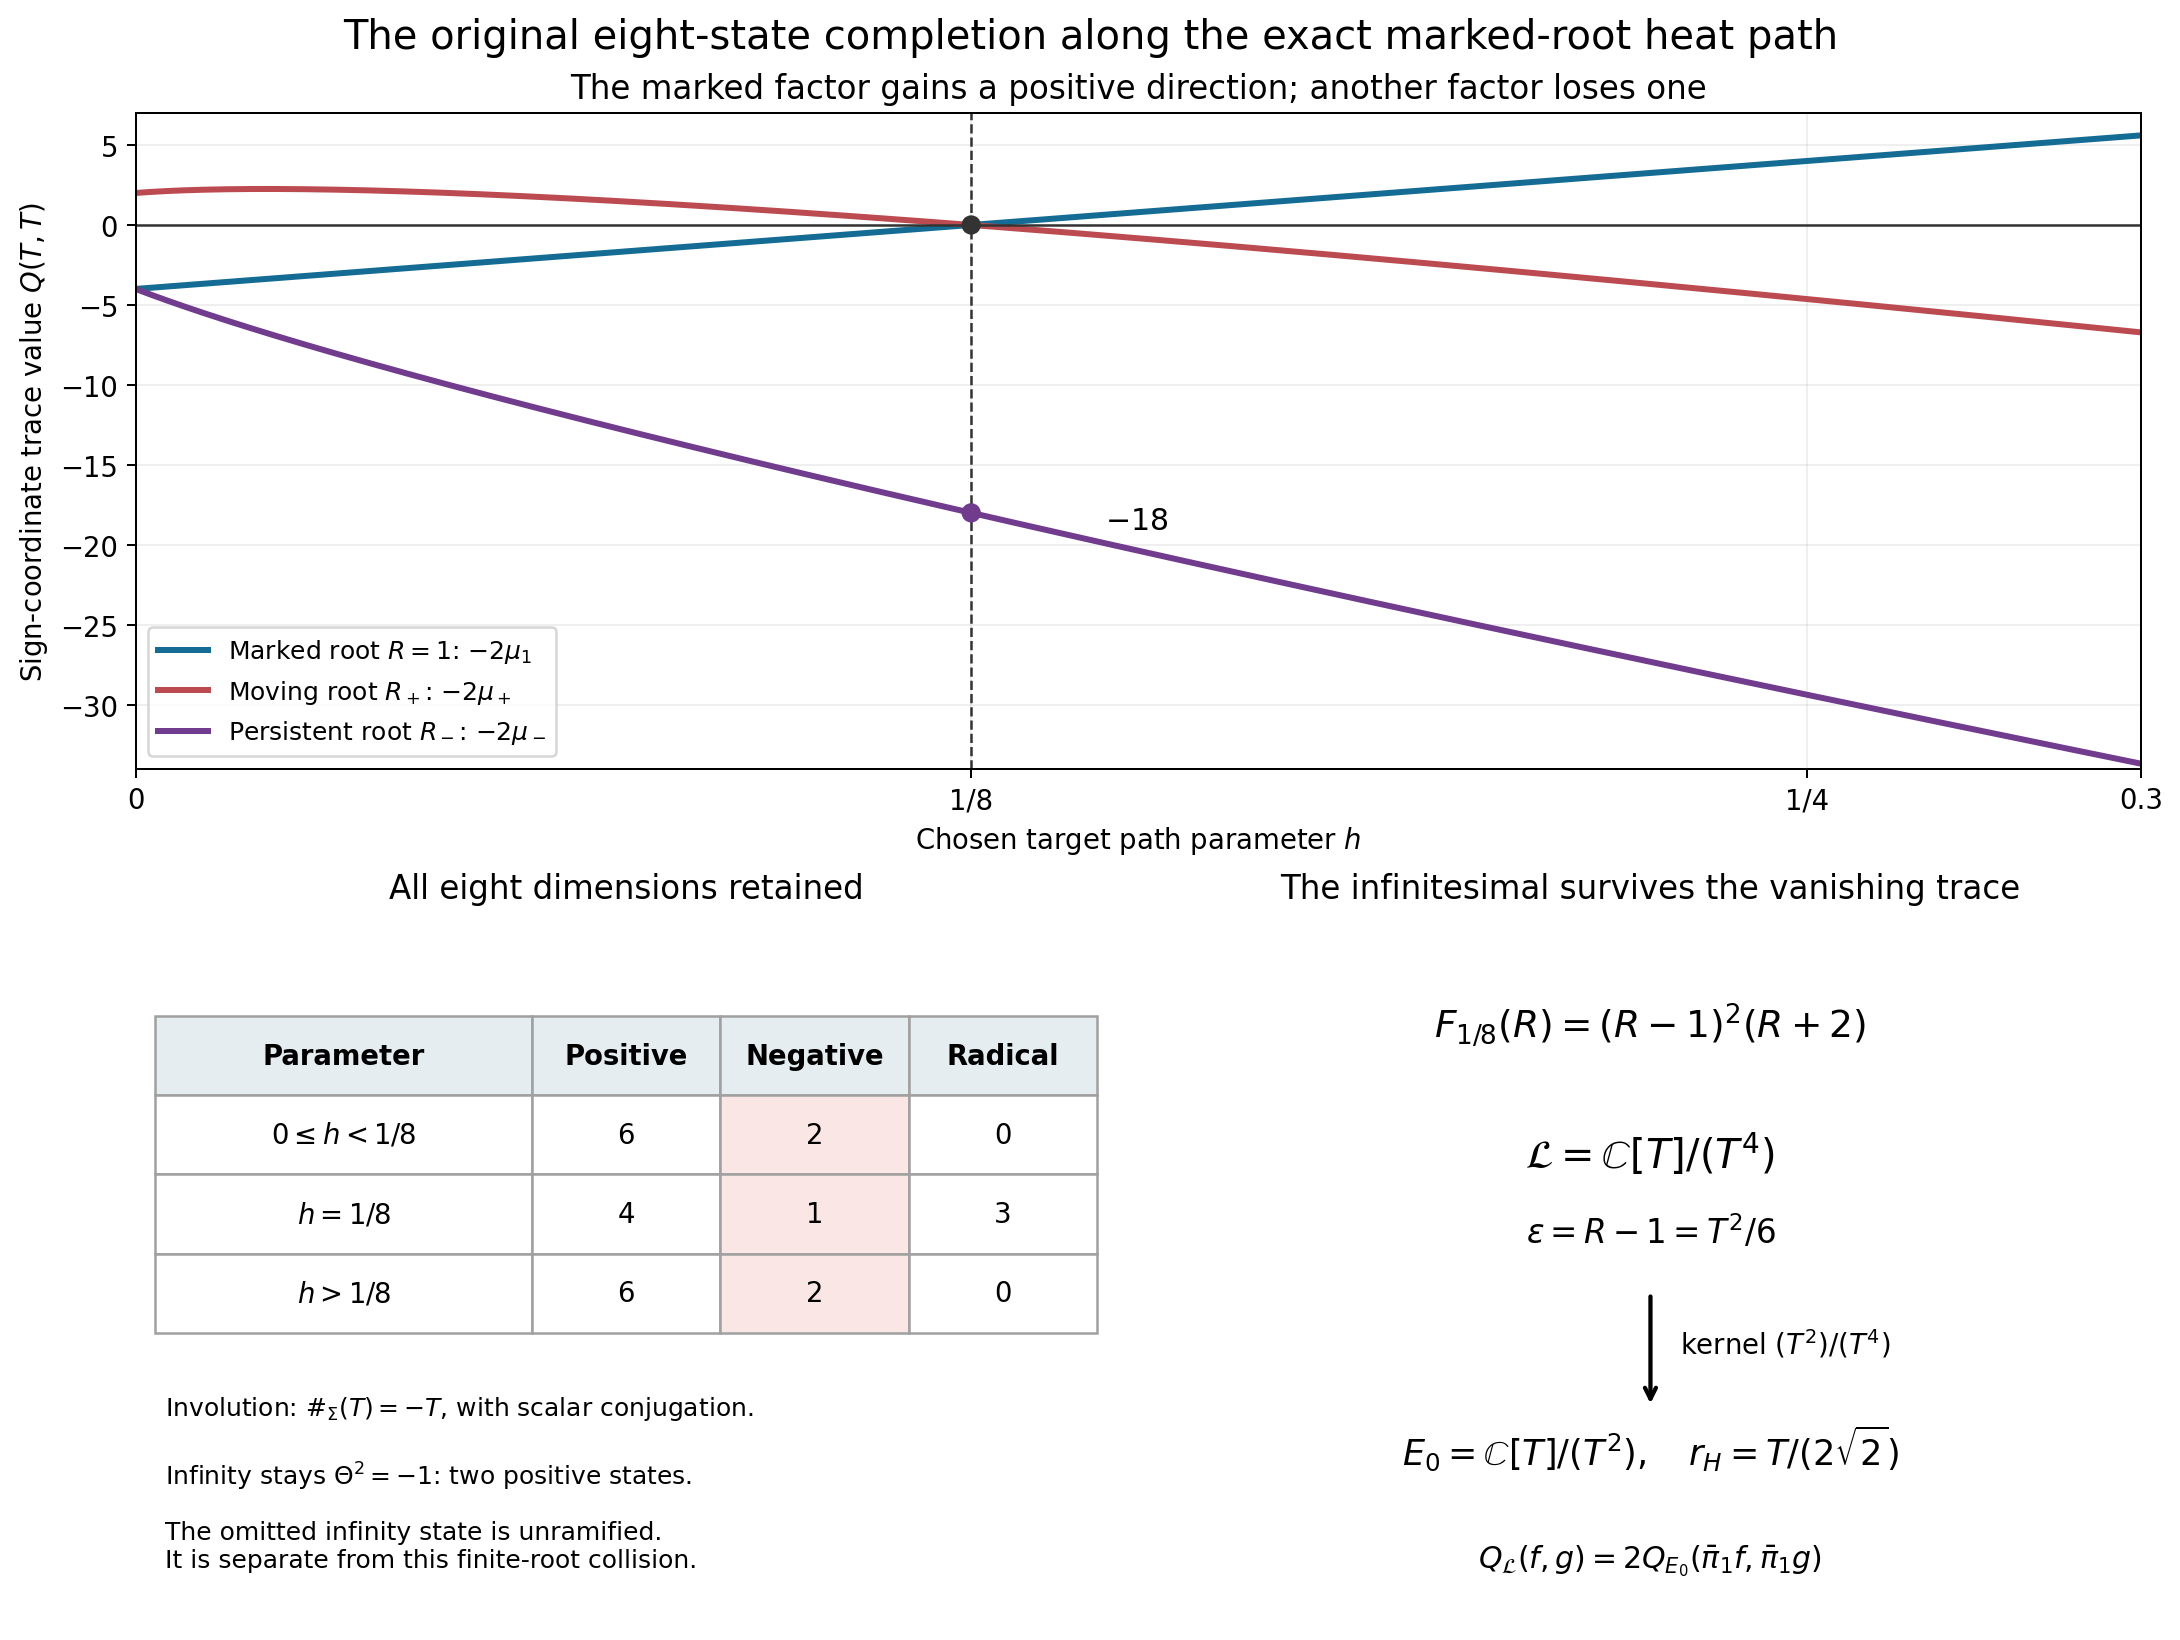
\includegraphics[keepaspectratio,alt={The full eight-state conjugate-deck trace along the specified target path. ESH35--ESH55 prove the three derivative functions, their sign exchange, the persistent negative factor, and the complete length-four collision with its dual-number quotient.}]{figures/30_eight_state_heat.png}}
\caption{The full eight-state conjugate-deck trace along the specified
target path. ESH35--ESH55 prove the three derivative functions, their
sign exchange, the persistent negative factor, and the complete
length-four collision with its dual-number quotient.}
\end{figure}

\clearpage

\section{The supported-zero prime in the full theta and Weil trace
distribution}\label{the-supported-zero-prime-in-the-full-theta-and-weil-trace-distribution}

\textbf{Original-zeta receiving calculation.} The working meromorphic
function is the original Riemann zeta, with its full Gamma/endpoints
multiplier and its full trivial-zero and pole divisor retained.
\href{FAITHFUL_THETA_COMPLETION_RETURN.md}{TF1--42} proves the original
labelled theta inverse and the actual heat-image defect.
\href{FAITHFUL_UNCOMPLETED_ZETA_HEAT.md}{UZ1--53} proves every
exceptional-point fibre, jet, original-zeta heat term and reflection
orientation.
\href{ORIGINAL_ZETA_COMPACT_WEIL_RECONSTRUCTION.md}{OZC1--48} rederives
the compact contour and interval operator directly from zeta, including
the left-cutoff Gamma boundary, and specifies exactly which compensated
pairing the bounds concern.
\href{ORIGINAL_ZETA_HEAT_CONTACT_RECONSTRUCTION.md}{OZH1--49} rederives
the actual meromorphic heat, rational signed trace, compact-test domain,
contact drift and full causal arithmetic variation. The raw full divisor
and the compensated Weil receiver are linked by their displayed
correction, not identified. In particular the fixed-test trivial-zero
sum converges exactly at translations at least 1/32 and equals the
earlier R term; at zero translation it requires the proved cutoff
compensation. \href{ORIGINAL_ZETA_CAUCHY_RECONSTRUCTION.md}{OZK1--38}
reconstructs the original signed Cauchy trace, its full Gamma
correction, resonant finite parts, every finite matrix and its index,
and the complete local heat jets. Its invertible map retains the raw
trace and correction separately. These complete receiving proofs govern
the interpretation of the retained auxiliary calculations below.

This construction begins with the actual semiring \(G(\mathbb Z)\),
includes its supported-zero prime in the full theta sum, and constructs
an unconditional trace distribution with every fixed-support endpoint
retained. Its arithmetic spectral sector is the rational, unramified,
trivial-character sector relevant to the Riemann zeta function. It
proves the maps from actual Weil tests to theta functions, from theta
functions to their Mellin divisor receiver, and from the full supported
object to the arithmetic scalar receiver. The arithmetic projection of
carriers, the pushforward of functions, and the projection which forgets
a point-function component are different maps and are calculated
separately.

The resulting identity is a distributional trace identity on explicitly
constructed representations. It is not an assertion of the global
operator equality on Connes's adele-class Hilbert space: the original
source explicitly distinguishes its unconditional explicit formula from
that further equality. The full supported trace, its scalar arithmetic
observation, and its Fourier-closed endpoint enlargement are all given
below.

Sources read for this derivation: the complete programme calculations
\href{https://github.com/KokunoYumeto/zeta-function-research-reader/blob/adfbfe74fa49e31cb7aa068cf755fb083be37c32/workbenches/splitzero-tandem/branches/tau-zero-prime-positivity/supporting_proofs/TAU_PRIME_SPECTRUM_DERIVATION.md}{the
complete tau prime spectrum derivation proof} (TPS1--TPS59),
\href{https://github.com/KokunoYumeto/zeta-function-research-reader/blob/adfbfe74fa49e31cb7aa068cf755fb083be37c32/workbenches/splitzero-tandem/branches/tau-zero-prime-positivity/supporting_proofs/TAU_CONNES_ENDPOINT_DERIVATION.md}{the
complete tau connes endpoint derivation proof} (TC1--TC41, including
TC24a--d), and
\href{https://github.com/KokunoYumeto/zeta-function-research-reader/blob/adfbfe74fa49e31cb7aa068cf755fb083be37c32/workbenches/splitzero-tandem/branches/tau-zero-prime-positivity/supporting_proofs/FULL_SUPPORT_CONNES_DERIVATION.md}{the
complete full support connes derivation proof} (FL1--FL58);
\href{https://github.com/KokunoYumeto/zeta-function-research-reader/blob/ac168d55cbb400a6c8926a00d67909ba65646ac5/workbenches/splitzero-tandem/branches/identity-absorber-square/sources/17555345_11.tex}{the
original supported-zero prime theorem}, labels thm:prime\_ideals\_S,
thm:krull\_dim\_S and eq:maximal\_chain; and Alain Connes,
\href{https://arxiv.org/abs/math/9811068}{\emph{Trace formula in
noncommutative geometry and the zeros of the Riemann zeta function},
arXiv:math/9811068v1}. The original author TeX was read at lines
608--822, 1574--1735, 3398--3490, 4217--4416 and 4770--4906. Its
Appendix I (36)--(38) supplies the full Poisson formula; Appendix II
Theorem 6 is the unconditional explicit formula. Section VI explicitly
calls its proposed global operator trace formal. The new maps and all
extra support terms below are derived, rather than inferred from the
prime spectrum alone.

\subsection{1. The prime and its actual arithmetic
maps}\label{the-prime-and-its-actual-arithmetic-maps}

Write \[
S=G(\mathbb Z)=\{\tau\}\sqcup\mathbb Z^\bullet,
\qquad e=0^\bullet\ne\tau,
\] \[
m^\bullet+n^\bullet=(m+n)^\bullet,\quad
m^\bullet n^\bullet=(mn)^\bullet,\quad
x+\tau=x,\quad x\tau=\tau.
\tag{SZW1}
\] The prime element \(e\) is a nonunit and is different from the
semiring zero \(\tau\). Its principal ideal is \(P_e=(e)=\{\tau,e\}\). A
product belongs to this ideal precisely when one factor is unsupported
or the product of its two integer amplitudes is zero. Since the integers
are a domain, this forces one factor into \(P_e\). Likewise
\(P_\tau=\{\tau\}\) is prime because a product is unsupported precisely
when a factor is unsupported. All other primes are \[
P_p=\{\tau\}\cup(p\mathbb Z)^\bullet,
\qquad
P_\tau\subsetneq P_e\subsetneq P_p.
\tag{SZW2}
\] Here is a short exhaustive proof of the needed classification. An
ideal containing any supported integer contains \(e\), by multiplication
by \(e\). Its supported amplitudes are closed under integer
multiplication and additive inverses, since multiplication by
\((-1)^\bullet\) is allowed. They form an integer ideal, hence are
\(n\mathbb Z\); primeness is exactly primeness of that integer ideal.
The remaining ideal is \(P_\tau\). This proves (SZW2), including height
one for \(P_e\) and height two for every \(P_p\).

The two maps \[
\pi:S\to\mathbb Z,\quad \pi(\tau)=0,\ \pi(n^\bullet)=n,
\qquad
\chi:S\to\mathbb B,\quad \chi(\tau)=0,\ \chi(n^\bullet)=1
\tag{SZW3}
\] preserve both semiring operations, as direct substitution shows.
Their joint map is injective. Contraction under \(\pi\) sends the
ordinary generic prime \((0)\) to \(P_e\), and \((p)\) to \(P_p\). Its
image is the closed subspace \(V(e)\); \(D(e)=\{P_\tau\}\). These
assertions follow by testing containment of the generating element \(e\)
in (SZW2).

The diagonal ring maps give semiring maps
\(S\to G(\mathbb A_{\mathbb Q})\) and \(S\to G(\mathbb Z_p)\). If
\(\mathfrak n_v=\ker(\mathbb A_{\mathbb Q}\to\mathbb Q_v)\), with
\(\mathbb Q_\infty=\mathbb R\), then \[
\bigl(S\to G(\mathbb A_{\mathbb Q})\bigr)^{-1}
(\{\tau\}\cup\mathfrak n_v^\bullet)=P_e.
\tag{SZW4}
\] Indeed a rational integer has zero image in any local field exactly
when it is zero. At the integral prime \(p\), reduction instead gives
\(S\to G(\mathbb F_p)\to\mathbb F_p\), whose arithmetic zero fibre is
\(P_p\). Thus the adelic supported-zero strata retain their separate
place labels while contracting to the height-one prime \(P_e\). This is
the precise arithmetic connection used in the theta construction; it
does not identify \(e\) with \(\tau\).

\subsection{2. Full sums, orbital sums, and the supported-zero
operator}\label{full-sums-orbital-sums-and-the-supported-zero-operator}

Use the original self-dual additive measure: Lebesgue measure on
\(\mathbb R\), measure one for \(\mathbb Z_p\) at each finite place, and
hence covolume one for the diagonal \(\mathbb Q\) in its adele ring.
These are the measures in Connes's Appendix I (34)--(36); the displayed
constants are for these fixed measures. Let
\(\mathcal S_{\mathrm{ev}}(\mathbb R)\) denote the even complex Schwartz
functions, with Fourier transform \[
\mathcal F\phi(\xi)=\int_{\mathbb R}\phi(x)e^{-2\pi i x\xi}\,dx.
\tag{SZW5}
\] For \(x>0\), put \[
\Theta_e\phi(x)=\sum_{n\in\mathbb Z}\phi(nx),\qquad
P\phi(x)=\sum_{n\in\mathbb Z\setminus\{0\}}\phi(nx),\qquad
a=\phi(0),\quad b=\int_{\mathbb R}\phi.
\tag{SZW6}
\] The full supported sum is \(\Theta_e\phi=P\phi+a\). It counts the
element \(e\) exactly once. For every compact interval of positive
\(x\), the sums and their derivatives converge absolutely and uniformly:
differentiating a term introduces a polynomial power of \(n\), which is
dominated by a higher Schwartz decay bound. For \(x\ge1\), the same
estimate gives \(P\phi(x)=O_N(x^{-N})\) for every \(N>1\). The assertion
also holds for all its derivatives and for \(\mathcal F\phi\).

Poisson summation in the stated Fourier convention gives the exact
formulas \[
\Theta_e\phi(x)=x^{-1}\Theta_e(\mathcal F\phi)(x^{-1}),
\] \[
P\phi(x)=x^{-1}P(\mathcal F\phi)(x^{-1})+b/x-a.
\tag{SZW7}
\] For the first formula apply Poisson to \(y\mapsto\phi(xy)\), whose
Fourier transform is \(x^{-1}(\mathcal F\phi)(\xi/x)\). Removing
precisely the zero-index term on both sides gives the second. Thus the
two endpoint coefficients are the value at the supported zero and its
Fourier dual, with their full signs retained.

The operator corresponding to multiplication by the supported zero also
has an exact domain. On \(\mathcal S(\mathbb R)+\mathbb C1\),
precomposition with the integer map \(x\mapsto nx\) is defined for every
\(n\in\mathbb Z\). For \(n=0\) it is \[
U_e\phi=\phi(0)1,\qquad U_e^2=U_e.
\tag{SZW8}
\] It has rank one on this space. It is not an endomorphism of the
Schwartz subspace, because the nonzero constant function is not
Schwartz. Its Fourier-dual domain is
\(\mathcal S(\mathbb R)\oplus\mathbb C\delta_0\), on which the exact
operator is \[
\mathcal F U_e\mathcal F^{-1}(\psi+c\delta_0)
=\left(\int_{\mathbb R}\psi(x)\,dx+c\right)\delta_0.
\tag{SZW8a}
\] Indeed \(\mathcal F^{-1}(\psi+c\delta_0)=\mathcal F^{-1}\psi+c1\),
whose value at zero is \(\int\psi+c\). Applying \(U_e\) and then
\(\mathcal F\) gives the formula since \(\mathcal F1=\delta_0\). Its
restriction to the Schwartz summand is
\(\psi\mapsto(\int\psi)\delta_0\). These are different maps with
specified domains and targets, not an identification of a point-function
with a Dirac distribution.

For the complete two-point carrier, a function is
\((\phi,c)\in\mathcal S(\mathbb R)\oplus\mathbb C_\tau\), with value
\(c\) at \(\tau\). Its sum over the rational integer carrier is \[
\Theta_S(\phi,c;x)=\sum_{u\in G(\mathbb Z)}(\phi,c)(xu)
=\Theta_e\phi(x)+c.
\tag{SZW9}
\] This converges by (SZW6); the unsupported point is counted once. The
contracted convention that an unsupported point contributes no value is
the exact invariant subspace \(c=0\), on which (SZW9) is the full
supported sum \(\Theta_e\phi\), still including \(e\).

This carrier sum is different from evaluating an orbital sum at a fixed
point. For \(\mathbb Q^\times\) acting on \(G(\mathbb A_{\mathbb Q})\),
both \(e\) and \(\tau\) are fixed, separately. Hence
\(\sum_{q\in\mathbb Q^\times}F(qe)\) is an infinite repetition of
\(F(e)\), and converges only when that value is zero; the corresponding
statement at \(\tau\) involves its independent value. The convergence
assertion follows because a nonzero constant sequence cannot tend to
zero. In contrast, for an idele \(x\),
\(\sum_{q\in\mathbb Q^\times}f(qx)\) samples no zero point and converges
by Schwartz decay and the compact support of its finite adelic factors.
On the spherical input \(f=\phi\otimes1_{\widehat{\mathbb Z}}\) and
idele \((x,1,1,\ldots)\), its contributing rationals are exactly the
nonzero integers, so it is precisely \(P\phi(x)\). This supplies the
actual map from the adelic orbital sum to (SZW6).

\subsection{3. Full finite support and its Poisson
defect}\label{full-finite-support-and-its-poisson-defect}

For the actual finite bounded distributive support lattice \(L\), write
\[
G_L(A)=\{(a,1_L):a\in A\}\cup\{z_\lambda=(0,\lambda):\lambda\ne1_L\},
\quad \tau_L=z_{0_L},\quad e_L=z_{1_L}.
\tag{SZW10}
\] Addition uses amplitude addition and support join; multiplication
uses amplitude multiplication and support meet. No nonzero amplitude is
placed at a nontop support. Let \(n=|L|\), and prescribe the function
space \[
\mathcal F_L=\mathcal S_{\mathrm{ev}}(\mathbb R)
\oplus\bigoplus_{\lambda\ne1_L}\mathbb C\delta_\lambda,
\qquad F=(\phi,(c_\lambda)),\quad C(F)=\sum_{\lambda\ne1_L}c_\lambda.
\tag{SZW11}
\] This is the global fixed-sector carrier of FL1--FL12. It is not the
coordinatewise carrier \(Q_F=\prod_{v\in F}G(k_v)\) of TC32--TC41. That
latter carrier has positive-dimensional strata \(\prod_{v\in E}k_v\),
whose integration characters are \(\chi_E(j)=\prod_{v\in E}|j_v|_v\), as
a change of variables in each coordinate proves. The exact inclusion
\(G(\prod_{v\in F}k_v)\to Q_F\) retains only the full-support stratum
and the all-unsupported point; restriction of functions to these is the
projection of TC41, with kernel the sum of all nonempty proper strata.
No such stratum, or its distinct integration character, has been
replaced here by a fixed line. The extra weight-one partners constructed
in Section 9 are explicitly new Fourier partners of the FL fixed lines.

Here \(\delta_\lambda\) is a point-function on the support carrier, not
a tempered Dirac distribution. The full sum and the componentwise
Fourier map are \[
\Theta_L(F;x)=P\phi(x)+a+C(F),\qquad
\mathcal F_L^{\mathrm{raw}}(\phi,c)=(\mathcal F\phi,c).
\] \[
\Theta_L(F;x)-x^{-1}\Theta_L(\mathcal F_L^{\mathrm{raw}}F;x^{-1})
=C(F)(1-x^{-1}).
\tag{SZW12}
\] Every equality follows by inserting (SZW7); thus the extra fixed
constants give an exact Poisson defect. They are not extra terms in the
punctured sum. With all support labels retained, the defect has
coefficients \(c_\lambda(1-x^{-1})\) on the respective nontop labels, so
cancellation in the scalar sum \(C(F)\) does not remove the labelled
defect.

On this space the dilation convention inherited from Connes is
\((V(u)\phi)(x)=\phi(x/u)\), \(u>0\); all \(c_\lambda\) are fixed. Its
endpoint map is onto: \[
E_L(F)=\left(a,b,(c_\lambda)_{\lambda\ne1_L}\right),\qquad
B_L=\mathbb C(0)_{e}\oplus\mathbb C(1)_{e^\vee}
\oplus\bigoplus_{\lambda\ne1_L}\mathbb C(0)_\lambda.
\tag{SZW13}
\] The notation \(\mathbb C(s)\) means the character \(u\mapsto u^s\).
Evaluation is invariant and \(\int\phi(x/u)dx=u\int\phi\), proving these
weights. Surjectivity of the original two endpoints follows, for
example, by taking one even Schwartz function with nonzero value at zero
and an even Schwartz function vanishing there but having nonzero
integral, then solving the resulting triangular two-by-two system. The
point coefficients give the other coordinate preimages independently.
The kernel is exactly \(\phi(0)=\int\phi=0\), with every extra
coefficient zero.

\subsection{4. Mellin regularization retains two different boundary
operations}\label{mellin-regularization-retains-two-different-boundary-operations}

For \(\Re s>1\), the punctured Mellin integral converges absolutely and
is \[
Z_\phi(s)=\int_0^\infty P\phi(x)x^s\frac{dx}{x}
=2\zeta(s)\int_0^\infty\phi(x)x^s\frac{dx}{x}.
\tag{SZW14}
\] Indeed at zero (SZW7) bounds the integrand by a constant times
\(x^{\Re s-1}+x^{\Re s}\), and at infinity it decreases arbitrarily
fast. Termwise integration is justified by the sum of absolute values;
replacing \(x\) by \(nx\) then gives the displayed Dirichlet series.
Evenness accounts for the factor two.

Splitting at one and using (SZW7) proves the complete continuation \[
\begin{aligned}
Z_\phi(s)={}&\int_1^\infty P\phi(x)x^s\frac{dx}{x}
+\int_1^\infty P(\mathcal F\phi)(x)x^{1-s}\frac{dx}{x}
+\frac{b}{s-1}-\frac{a}{s}.
\end{aligned}
\tag{SZW15}
\] Both integrals are entire: on every compact set of \(s\), every
differentiated integrand is dominated by a sufficiently high inverse
power of \(x\), times a power of \(\log x\). The residues are exactly
\(-a\) at zero and \(b\) at one. Formula (SZW15) has kept the full
supported-zero and dual endpoint coefficients.

The full function \(\Theta_L(F;x)\) usually has no Mellin convergence
strip. Its asymptotic terms are \[
\Theta_L(F;x)=a+C(F)+O_N(x^{-N})\quad(x\to\infty),
\] \[
\Theta_L(F;x)=b/x+C(F)+O_N(x^N)\quad(x\downarrow0).
\tag{SZW16}
\] The second estimate follows from (SZW7), increasing its Schwartz
exponent by one. Define its meromorphic finite part by subtracting these
terms on the two half-lines, integrating the remaining rapidly
decreasing functions, and adding the meromorphic continuations of the
subtracted elementary integrals. The elementary contributions are \[
\frac{b}{s-1}+\frac{C(F)}s-\frac{a+C(F)}s
=\frac{b}{s-1}-\frac as.
\tag{SZW17}
\] Here \(\int_0^1x^{s-1}dx=1/s\) initially for \(\Re s>0\), while
\(\int_1^\infty x^{s-1}dx=-1/s\) initially for \(\Re s<0\). The equality
of their meromorphic continuations does not posit a common domain of
ordinary convergence. Thus the full finite part is exactly (SZW15). In
particular deleting the small-end term \(C(F)/s\) while retaining its
large-end counterpart would introduce a spurious pole.

The cancellation in (SZW17) is not the trace of a fixed representation.
To see the retained distribution, use \(t=\log x\) and Fourier
convention \(\widehat h(u)=\int h(t)e^{-iut}dt\). For a constant \(c\),
its exponentially damped Fourier transform is \[
\int_{\mathbb R}c e^{-\varepsilon|t|}e^{-iut}dt
=\frac{c}{\varepsilon+iu}+\frac{c}{\varepsilon-iu}
=\frac{2c\varepsilon}{\varepsilon^2+u^2}
\ \longrightarrow\ 2\pi c\delta_0(u)
\tag{SZW18}
\] in tempered distributions as \(\varepsilon\downarrow0\). For proof,
pair the last expression with a Schwartz function \(g\), substitute
\(u=\varepsilon v\), and apply dominated convergence to
\(2c\int g(\varepsilon v)/(1+v^2)dv\). Its limit is \(2\pi c g(0)\). The
integral \(\int(1+v^2)^{-1}dv=\pi\) follows from the antiderivative
\(\arctan v\). The fixed line therefore contributes the character
distribution \(h\mapsto\int h(t)dt\), even though its meromorphic
two-tail finite part is zero. These are two explicitly different
receiving maps from the same constant function. Each lower support
coefficient has its own copy of (SZW18).

\subsection{5. An exact map from admissible Weil tests to the full theta
object}\label{an-exact-map-from-admissible-weil-tests-to-the-full-theta-object}

Use precisely the existing HEB11 and WEC1 convention: \[
\mathcal T=C_c^\infty(\mathbb R;\mathbb C),\qquad
M_f(s)=\int_{\mathbb R}f(v)e^{-(s-1/2)v}dv,
\qquad f^\#(v)=\overline{f(-v)}.
\tag{SZW19}
\] Then \(M_{f^\#}(s)=\overline{M_f(1-\overline s)}\), by changing
variables. If the alternative plus-exponent convention is used, its
exact relation is \(M_f^+(s)=M_f(1-s)=M_{f(-\cdot)}(s)\); no convention
is silently interchanged.

Define a Gaussian dilation map with its complete amplitude: \[
\boxed{(J_\theta f)(x)=\int_{\mathbb R}e^{v/2}f(v)
\exp(-\pi e^{2v}x^2)\,dv.}
\tag{SZW20}
\] This is even Schwartz. Indeed the support of \(f\) bounds \(e^{2v}\)
above and below by positive constants. Every derivative in \(x\),
multiplied by every power of \(x\), is consequently bounded by an
integrable multiple of a Gaussian uniformly in \(v\). Differentiation
under the integral and the Schwartz estimates follow. Direct evaluation
and the Gaussian integral give \[
(J_\theta f)(0)=M_f(0),\qquad
\int_{\mathbb R}J_\theta f=M_f(1),\qquad
\mathcal F(J_\theta f)=J_\theta(f(-\cdot)).
\tag{SZW21}
\] For the second equality, the Gaussian has integral \(e^{-v}\). For
the third, its Fourier transform is \(e^{-v}\exp(-\pi e^{-2v}\xi^2)\);
substituting \(v\mapsto-v\) gives the formula. Consequently
\(J_\theta(f^\#)=\mathcal F\overline{J_\theta f}\). This is an actual
intertwining map between the test involution and the supported-zero
Fourier boundary, not only an equality of two pairs of numbers.

The Mellin calculation, first for \(\Re s>1\), is \[
\int_0^\infty (J_\theta f)(x)x^s\frac{dx}{x}
=\frac12\pi^{-s/2}\Gamma(s/2)M_f(s),
\] \[
\boxed{Z_{J_\theta f}(s)=\Lambda(s)M_f(s),\qquad
\Lambda(s)=\pi^{-s/2}\Gamma(s/2)\zeta(s).}
\tag{SZW22}
\] The first integral already converges for \(\Re s>0\). Compactness of
the \(v\)-support and Gaussian decay justify Fubini, and
\(x\mapsto e^{-v}x\) gives the factor \(e^{-sv}\). The second formula
follows from (SZW14) and continues meromorphically by (SZW15). It
retains the full amplitude \(M_f\). Its residues are \(-M_f(0)\) and
\(M_f(1)\), exactly the endpoint map (SZW21).

The two endpoint values range independently over \(\mathbb C^2\). For an
explicit section choose a nonnegative even nonzero bump
\(\psi\in\mathcal T\), put \(b_\psi=M_\psi(0)=M_\psi(1)>0\), and let
\(\psi_t(v)=\psi(v-t)\), with \(t=\log4\). Then \[
f_{A,B}=\frac{4B-A}{3b_\psi}\psi
+\frac{2(A-B)}{3b_\psi}\psi_t,
\qquad (M_{f_{A,B}}(0),M_{f_{A,B}}(1))=(A,B).
\tag{SZW23}
\] The translated bump has endpoints \((2b_\psi,b_\psi/2)\), which
verifies both identities. Thus no universal restriction such as \(A=B\),
or invariance under an auxiliary finite group, follows merely from
admissibility of these Weil tests. Its exact endpoint kernel is
\(\{f:M_f(0)=M_f(1)=0\}\), and (SZW23) splits its quotient as a vector
space.

\subsection{6. The complete arithmetic explicit formula, derived with
these
endpoints}\label{the-complete-arithmetic-explicit-formula-derived-with-these-endpoints}

For \(h\in\mathcal T\), set \(H(s)=M_h(s)\),
\(\widehat h(t)=\int h(v)e^{-itv}dv\), and let \(\rho\) range over all
nontrivial zeros of \(\zeta\), with their multiplicities \(m_\rho\).
Define \[
\begin{aligned}
Z(h)&=\sum_\rho m_\rho H(\rho),\\
A_\infty(h)&=\frac1{2\pi}\int_{\mathbb R}\widehat h(t)
\bigl(\Re\psi(1/4+it/2)-\log\pi\bigr)dt,\\
P_{\mathrm{fin}}(h)&=\sum_{p}\sum_{k\ge1}
(\log p)p^{-k/2}\{h(k\log p)+h(-k\log p)\}.
\end{aligned}
\tag{SZW24}
\] Here \(\psi=\Gamma'/\Gamma\) is the digamma function, not the bump
used above. The last sum is finite for any particular compactly
supported \(h\). The archimedean integral is absolutely convergent since
\(\widehat h\) decreases faster than every inverse power and the digamma
factor grows at most logarithmically. The zero sum is absolutely
convergent; a proof of the requisite bound is included below.

The exact identity is \[
\boxed{Z(h)=H(0)+H(1)+A_\infty(h)-P_{\mathrm{fin}}(h).}
\tag{SZW25}
\] The boundary \(H(0)+H(1)\) here is obtained from the actual full
supported theta (SZW7), (SZW15), and (SZW22). It has not been deleted
and then replaced by a numerical Euler factor for \(e\).

Here are the analytic details and signs. For the Gaussian
\(g(x)=e^{-\pi x^2}\), (SZW15) gives \(Z_g=\Lambda\), simple poles at
\(0,1\) with residues \(-1,1\), and the functional equation
\(\Lambda(s)=\Lambda(1-s)\). The entire function
\(\xi(s)=\tfrac12s(s-1)\Lambda(s)\) therefore has \(\xi(0)=\xi(1)=1/2\).
Its theta integral also gives
\(\max_{|s|\le R}|\xi(s)|\le\exp(CR\log(R+2))\) for some fixed \(C\):
bound the rapidly decreasing Gaussian tail by \(C_0e^{-c x^2}\) and each
power in the two integrals by \(x^{R+1}\); its integral is bounded by a
constant times \(c^{-(R+1)/2}\Gamma((R+1)/2)\). The elementary Stirling
bound for the positive real Gamma function gives the claimed estimate.
Jensen's formula then implies that the number of zeros in \(|s|\le R\),
counted with multiplicity, is \(O(R\log(R+2))\), by applying it on
radius \(2R\) around the nonzero value at zero.

The Euler product is nonzero in \(\Re s>1\). It follows from the
functional equation that \(\xi\) has no zeros in \(\Re s<0\). For
completeness the boundary line \(\Re s=1\) has no zeros either. For
\(\sigma>1\), the logarithm of
\(\zeta(\sigma)^3|\zeta(\sigma+it)|^4|\zeta(\sigma+2it)|\) is a
convergent sum of the nonnegative terms
\(2p^{-k\sigma}(1+\cos(kt\log p))^2/k\). The product is therefore at
least one. If \(t\ne0\) and \(\zeta(1+it)\) were a zero of order at
least one, analyticity there, finiteness at \(1+2it\), and the simple
pole at one would make that product tend to zero as
\(\sigma\downarrow1\), a contradiction. The functional equation excludes
zeros on \(\Re s=0\); \(\xi(0),\xi(1)\ne0\) handle the two real
endpoints. Thus all zeros counted above lie in \(0<\Re s<1\).

Repeated integration by parts in (SZW19) gives
\(|H(\sigma+it)|\le C_{N,I}(1+|t|)^{-N}\) for every \(N\), uniformly on
each fixed bounded real interval \(I\) for \(\sigma\). Together with the
zero count, this proves absolute convergence of \(Z(h)\).

Set \(\ell=\Lambda'/\Lambda\). Integrate \(\ell(s)H(s)\) around the
rectangle with vertical sides \(-1,2\), oriented positively. The residue
theorem gives the zeros minus \(H(0)+H(1)\); the residues of \(\ell\) at
its two poles are \(-1\), independently of the pole residues of
\(\Lambda\). A sequence of upper and lower heights tending to infinity
can be chosen so that the horizontal integrals tend to zero. One precise
justification is the genus-one Hadamard factorization of the
order-at-most-one entire function \(\xi\). It gives
\(\xi'/\xi(s)=B+\sum_\rho m_\rho((s-\rho)^{-1}+\rho^{-1})\), locally
normally away from zeros. The zero bound above implies
\(\sum m_\rho/|\rho|^2<\infty\). In each interval \([N,N+1]\), exclude
intervals of radius \(N^{-3}\) around the imaginary parts of zeros with
\(|\rho|\le3N\). Their total length is \(O(N^{-2}\log N)<1\), so a
remaining height exists. On that horizontal segment every nearby
denominator has modulus at least \(N^{-3}\), yielding a polynomial bound
\(O(N^4\log N)\) for the finite part of the sum. The tail is
\(O(\log N)\), since the paired summand is bounded by \(C N/|\rho|^2\).
The same argument applies below the real axis. Subtracting
\(1/s+1/(s-1)\) gives the same polynomial bound for \(\ell\). The
arbitrarily high inverse-power decay of \(H\) proves the asserted
disappearance of the horizontal integrals. This argument uses the
classical Hadamard and Jensen theorems of complex analysis, with their
hypotheses verified here; it does not assume the Riemann hypothesis or
any zero-location assertion beyond the strip proved above.

Since \(\ell(1-s)=-\ell(s)\), changing variables on the left edge now
gives \[
Z(h)-H(0)-H(1)=\frac1{2\pi i}\int_{\Re s=2}
\ell(s)\{H(s)+H(1-s)\}\,ds.
\tag{SZW26}
\] Insert
\(\ell(s)=-\tfrac12\log\pi+\tfrac12\psi(s/2)-\sum_{p,k}(\log p)p^{-ks}\).
The prime series converges absolutely on this line. Fourier inversion in
each term gives respectively \(p^{-k/2}h(-k\log p)\) and
\(p^{-k/2}h(k\log p)\); this proves its contribution is
\(-P_{\mathrm{fin}}\). The Gamma part is holomorphic for \(\Re s>0\), so
its line can be shifted to \(1/2\). Combining the second term after
\(t\mapsto-t\) gives \(-\log\pi+\Re\psi(1/4+it/2)\), proving its
contribution is \(A_\infty\). This proves (SZW25) with the exact signs,
constants and domains in (SZW24).

The same identity is Connes's Appendix II Theorem 6 in the unramified
trivial-character sector. Its test on \(C_{\mathbb Q}\) is exactly \[
q_h(j)=|j|^{-1/2}h(-\log|j|),\qquad
\widehat q_h(s)=\int_{C_{\mathbb Q}}q_h(j)|j|^s d^*j=H(s),
\tag{SZW27}
\] where the norm-one compact group has Haar mass one and the norm
quotient has measure \(du/u\). The equality follows by \(v=-\log|j|\).
The local distribution on the other side is consequently
\(P_{\mathrm{fin}}-A_\infty\), with all the source principal-value
conventions fixed by this equality and by the stated self-dual additive
Fourier character. The finite-prime coefficients have remained
\((\log p)p^{-k/2}\); none was changed to \(\log(p+1)\).

\subsection{7. An actual summable divisor trace, with the theta image
and its cokernel
mapped}\label{an-actual-summable-divisor-trace-with-the-theta-image-and-its-cokernel-mapped}

The zero trace in (SZW24) has an unconditional operator realization that
retains every multiplicity. It is a divisor receiver constructed from
\(\Lambda\) in (SZW22), not an assumed identification with the entire
original adele-class Hilbert space.

Let \(\mathcal O\) be the ring of entire functions of \(s\), put
\(q_0(s)=s(s-1)\), and let \(\mathcal O(P)=q_0^{-1}\mathcal O\) be the
meromorphic functions with at most simple poles at \(0,1\).
Multiplication gives the injective map \[
\mathcal O\xrightarrow{\times\Lambda}\mathcal O(P),\qquad
q_0\Lambda=2\xi.
\tag{SZW28}
\] Its injectivity follows because \(\Lambda\) is not identically zero.
The map \(F\mapsto q_0F\) identifies its cokernel with
\(\mathcal O/(2\xi)\). The other exact quotient is \[
0\to\mathcal O\to\mathcal O(P)
\xrightarrow{(\operatorname{Res}_0,\operatorname{Res}_1)}\mathbb C^2\to0.
\tag{SZW29}
\] Surjectivity is witnessed by \(a/s+b/(s-1)\), and a member with both
residues zero is entire. Multiplication by \(H\) on this quotient is
diagonal with values \(H(0),H(1)\). By (SZW22), the actual theta map
\(f\mapsto Z_{J_\theta f}=\Lambda M_f\) lands in the image of (SZW28);
its residue map is \(f\mapsto(-M_f(0),M_f(1))\). This proves both the
zero-cokernel vanishing of the theta image and the nonvanishing of its
independent endpoint data.

At a zero \(\rho\) of multiplicity \(m_\rho\), the local cokernel is \[
\mathcal J_\rho=\mathbb C[z]/(z^{m_\rho}),\qquad z=s-\rho.
\tag{SZW30}
\] Indeed \(2\xi(s)=(s-\rho)^{m_\rho}u_\rho(s)\) with a holomorphic unit
\(u_\rho(\rho)\ne0\), and division by that unit gives the stated
quotient. The global jet map has the explicit product target \[
\mathcal O(P)\longrightarrow\prod_\rho\mathcal J_\rho,
\qquad F\longmapsto\bigl([q_0F]_{\rho,m_\rho}\bigr)_\rho.
\tag{SZW30a}
\] Its kernel is exactly \(\Lambda\mathcal O\): vanishing of every
required jet makes \(q_0F/(2\xi)\) entire at every zero and elsewhere,
proving the reverse inclusion as well as the forward one. Every finitely
supported tuple of jets occurs. For one chosen \(\rho\), the entire
function \(2\xi(s)/(s-\rho)^{m_\rho}\) vanishes with the required orders
at every other zero and is a unit at \(\rho\). Multiply it by the Taylor
polynomial of the desired jet divided by that unit, of degree below
\(m_\rho\), and then divide by \(q_0\). This gives the prescribed jet
and zero jets elsewhere. Finite sums give the general finite tuple.
These are explicit maps into and out of the divisor receiver, preserving
the theta amplitude in (SZW22).

In particular, put \(\mathcal C=\mathcal O(P)/\Lambda\mathcal O\), let
\(\iota:\mathcal C\hookrightarrow\prod_\rho\mathcal J_\rho\) be the
induced injective map, and define \[
\mathcal C_{\mathrm{fin}}
=\iota^{-1}\!\left(\bigoplus_\rho^{\mathrm{alg}}\mathcal J_\rho\right).
\qquad
\iota:\mathcal C_{\mathrm{fin}}\xrightarrow{\ \sim\ }
\bigoplus_\rho^{\mathrm{alg}}\mathcal J_\rho.
\tag{SZW30b}
\] The superscript denotes the algebraic direct sum, consisting of
finite tuples. The preceding interpolation proves this isomorphism. The
Hilbert space used next is the completion of this particular subspace
with its displayed jet norms. No identification of the entire analytic
cokernel or the full product with that Hilbert space is asserted.

Give each \(\mathcal J_\rho\) the Euclidean norm in its full basis
\((1,z,\ldots,z^{m_\rho-1})\), and form their Hilbert direct sum
\(\mathcal H_Z\). Multiplication by \(u^{\rho+z}\), \(u>0\), defines a
bounded representation: if \(N_\rho\) is multiplication by \(z\), then
\(\|N_\rho\|\le1\), and \[
\|u^\rho\exp((\log u)N_\rho)\|
\le\max(1,u)e^{|\log u|}
\tag{SZW31}
\] uniformly in \(\rho\). The bound and density of vectors in finitely
many summands prove strong continuity. Integrating against \(q_h\) gives
multiplication by the full jet of \(H\). This operator is trace class.
To verify this directly, if \(\operatorname{supp}h\subset[-R,R]\),
repeated integration by parts in
\(H^{(k)}(\rho)/k!=\int(-v)^kh(v)e^{-(\rho-1/2)v}dv/k!\) gives, after
summing over all \(k\ge0\), a bound
\(\sum_k|H^{(k)}(\rho)|/k!\le C_{N,h}(1+|\Im\rho|)^{-N}\). The summation
is justified because \(\sum_k|v|^k/k!=e^{|v|}\), and each fixed-order
derivative of the series of absolute derivative bounds remains bounded
on the compact interval; the extra falling factorial factors in \(k\)
are absorbed by this same exponential series. The real part of \(\rho\)
is in \([0,1]\), so it introduces only uniform constants. The trace norm
of the multiplication matrix is at most
\(m_\rho\sum_k|H^{(k)}(\rho)|/k!\). Summing over zeros converges by the
count proved above, taking \(N>2\).

Its trace is therefore the absolutely convergent sum \[
\operatorname{Tr}_{\mathcal H_Z}(q_h)=\sum_\rho m_\rho H(\rho)=Z(h).
\tag{SZW32}
\] Every nilpotent jet is retained in (SZW30); the trace of its positive
powers is zero because their multiplication matrices have zero diagonal.
This is not a quotient identifying such a jet with \(\tau\), or even
with the supported amplitude zero.

Reflection has the exact maps \(\rho\mapsto\rho^\#=1-\overline\rho\) and
\(p(z)\mapsto\overline{p(-\overline z)}\) from \(\mathcal J_\rho\) to
\(\mathcal J_{\rho^\#}\). The functional equation and reality of \(\xi\)
give equal multiplicities, so these maps are defined and square to the
identity. At the global analytic level the same map is
\(F^\#(s)=\overline{F(1-\overline s)}\). The identities \(q_0^\#=q_0\)
and \(\Lambda^\#=\Lambda\) show that it preserves \(\mathcal O(P)\) and
\(\Lambda\mathcal O\), descends to \(\mathcal C\), and intertwines
(SZW30a). It preserves \(\mathcal C_{\mathrm{fin}}\), and its jet map
extends to an antilinear isometry \(J_Z\) of \(\mathcal H_Z\), since
coefficient conjugation and multiplication of the degree-\(k\)
coefficient by \((-1)^k\) preserve the displayed Euclidean norms. Its
exact dilation covariance is \[
J_ZU_Z(u)=u\,U_Z(u^{-1})J_Z,
\qquad u>0.
\tag{SZW32a}
\] Indeed the reflected multiplier in the \(\rho^\#\) summand is
\(u^{\overline\rho-z}=u\,u^{-\rho^\#-z}\), proving the identity on every
full jet and hence on the Hilbert completion. This is an
anti-intertwiner between dilation and reflected dilation; it is not a
claim that the dilation generator is self-adjoint for a positive Weil
form. All derivative coordinates remain present.

\subsection{8. The full supported trace identity and its exact scalar
observations}\label{the-full-supported-trace-identity-and-its-exact-scalar-observations}

For a support label \(\lambda\), retain its coordinate vector
\(\mathbf e_\lambda\) in the vector space \(\mathbb C[L]\). Define the
label-resolved boundary, divisor, and geometric trace distributions by
their actual representation traces: \[
\begin{aligned}
\boldsymbol B_L(h)&=(H(0)+H(1))\mathbf e_{1_L}
+H(0)\sum_{\lambda\ne1_L}\mathbf e_\lambda,\\
\boldsymbol Z_L(h)&=Z(h)\mathbf e_{1_L},\\
\boldsymbol D_L(h)&=(P_{\mathrm{fin}}(h)-A_\infty(h))\mathbf e_{1_L}
+H(0)\sum_{\lambda\ne1_L}\mathbf e_\lambda.
\end{aligned}
\tag{SZW33}
\] The boundary trace is precisely that of (SZW13) integrated against
(SZW27); the zero trace is (SZW32); each lower-coordinate trace is the
fixed-character distribution (SZW18). Equivalently, take the finite even
representation \(B_L\) and the odd representation \(\mathcal H_Z\), with
their indicated labels. Their integrated operators are trace class, so
their label-resolved supertrace is well defined. Equation (SZW25) proves
the full identity \[
\boxed{\boldsymbol B_L-\boldsymbol Z_L=\boldsymbol D_L.}
\tag{SZW34}
\] Thus all terms come from defined test spaces, the actual full theta,
explicit fixed-coordinate representations, and the Mellin divisor
receiver. No assertion about an unconstructed global Hilbert trace is
used.

Two different scalar maps already give different observations. Let
\(\epsilon_{\mathrm{top}}\) pick the coefficient of \(\mathbf e_{1_L}\),
and let \(\epsilon_{\mathrm{all}}\) sum all coefficients. Then \[
\begin{aligned}
\epsilon_{\mathrm{top}}\boldsymbol D_L&=P_{\mathrm{fin}}-A_\infty,\\
\epsilon_{\mathrm{all}}\boldsymbol D_L&=P_{\mathrm{fin}}-A_\infty+(n-1)H(0),\\
\epsilon_{\mathrm{all}}\boldsymbol B_L&=nH(0)+H(1).
\end{aligned}
\tag{SZW35}
\] The first map forgets all lower fixed traces; the second retains
their sum. Their kernels on \(\mathbb C[L]\) are respectively the span
of the nontop coordinate vectors, and the hyperplane of zero coordinate
total. These maps must not be called the same arithmetic pushforward.

First take \(A=\mathbb R\), as in the function space (SZW11). The actual
carrier projection \(G_L(\mathbb R)\to\mathbb R\) identifies all zero
points. Its fibre-sum pushforward is \[
(\phi,c)\longmapsto\phi+C(F)1_{\{0\}},
\qquad
\mathcal F_L\longrightarrow
\mathcal S_{\mathrm{ev}}(\mathbb R)\oplus\mathbb C1_{\{0\}}.
\tag{SZW36}
\] The sum is direct because a continuous function on \(\mathbb R\)
supported only at zero is zero. Its kernel consists exactly of
\(\phi=0\) and \(\sum c_\lambda=0\). The subsequent map
\(\phi+d1_{\{0\}}\mapsto\phi\) is a separate projection, with kernel the
added point-function line. It is this composite which returns the
classical regular orbital observation. For \(L=\mathbb B\), the first
pushforward identifies the external coordinate with an independent point
correction at supported zero, while the second projection kills that
correction. Thus even in the two-point case the full trace and its
regular arithmetic observation are connected by two explicit maps.

There is also an adelic version with its own domain
\(\mathcal S(\mathbb A_{\mathbb Q})\oplus\mathbb C^{L\setminus\{1_L\}}\):
it sends \((f,c)\) to \(f+C(F)1_{\{0_{\mathbb A}\}}\) in
\(\mathcal S(\mathbb A_{\mathbb Q})\oplus\mathbb C1_{\{0_{\mathbb A}\}}\),
with exactly the same kernel proof since the adele group is nondiscrete.
The spherical embedding of (SZW11) is explicitly \[
(\phi,c)\longmapsto(\phi\otimes1_{\widehat{\mathbb Z}},c),
\qquad
(\phi,c)\longmapsto
\phi\otimes1_{\widehat{\mathbb Z}}+C(F)1_{\{0_{\mathbb A}\}}
\tag{SZW36a}
\] after that adelic pushforward. This states the real-to-adelic map
before adding the adelic point correction; the original real function
has not silently changed its domain.

More general support maps send point coefficients by finite fibre sums,
as in FL19. Separate Boolean branches record the total and the
principal-filter sums indexed by join-irreducibles. Their exact kernel
is \[
N_L=\{d:\sum_\lambda d_\lambda=0,\quad
\sum_{\lambda\ge j}d_\lambda=0\text{ for every join-irreducible }j\},
\tag{SZW37}
\] of dimension \(n-|J(L)|-1\). To verify the dimension, order the
join-irreducibles compatibly with their partial order and solve their
upper-triangular principal-filter system on the coordinate vectors at
those elements; the bottom coordinate then prescribes the total. This
gives surjectivity onto \(|J(L)|+1\) moments. The kernel is invariant
and trivial under dilation, so it contributes exactly
\((n-|J(L)|-1)H(0)\) to the endpoint trace before it is forgotten. All
full filter moments reconstruct the coefficients by finite Möbius
inversion, whose inverse follows by multiplying the two triangular
incidence matrices. Consequently these lost traces are actual labelled
objects, not a claim that equality of all pointwise branch labels gives
injectivity on their linear combinations.

\subsection{9. The reflected endpoint defect and its concrete Fourier
closure}\label{the-reflected-endpoint-defect-and-its-concrete-fourier-closure}

For \(f,g\in\mathcal T\), put \(h=f^\#*g\), using additive convolution.
Fubini gives \(M_h(s)=\overline{M_f(1-\overline s)}M_g(s)\). If
\(A_f=M_f(0)\) and \(B_f=M_f(1)\), then \[
H(0)=\overline{B_f}A_g,\qquad H(1)=\overline{A_f}B_g.
\tag{SZW38}
\] The supported-zero pair is therefore exactly
\(\overline{B_f}A_g+\overline{A_f}B_g\), the hyperbolic Hermitian plane
with matrix \(\begin{psmallmatrix}0&1\\1&0\end{psmallmatrix}\) on
\((A,B)\). It is not a positive form on all admissible tests; (SZW23)
supplies arbitrary endpoint pairs, including \((1,-1)\), of value
\(-2\).

The entire unreflected endpoint representation has instead \[
B_L(f,g)=n\overline{B_f}A_g+\overline{A_f}B_g,
\qquad
B_L-B_L^*=(n-1)(H(0)-H(1)).
\tag{SZW39}
\] The last equality is an equality of sesquilinear forms, obtained by
exchanging the inputs and conjugating. For \((A_f,B_f)=(1,i)\), its
diagonal value is \(-i(n-1)\), so for \(n>1\) it is not Hermitian. This
exact defect is also present in
\(\epsilon_{\mathrm{all}}\boldsymbol D_L\); (SZW34) therefore retains it
on both sides, instead of confusing it with the Hermitian divisor form
\(Z(f^\#*g)\).

The obstruction defines a concrete missing object. In tempered
distributions on \(\mathbb R\), let \[
B_L^{\mathcal F}=(\mathbb C1\oplus\mathbb C\delta_0)\otimes\mathbb C[L].
\tag{SZW40}
\] For dilation \(V(u)\phi(x)=\phi(x/u)\), extend the action to
distributions by
\(\langle V(u)T,\varphi\rangle=u\langle T,\varphi(u\cdot)\rangle\). This
agrees with the action on regular distributions by change of variables.
It fixes \(1\) and sends \(\delta_0\) to \(u\delta_0\), so the two
weights are precisely zero and one. Fourier interchanges these two
distributions. They are linearly independent: test against a compactly
supported smooth function vanishing at zero but having nonzero integral
to determine the constant coefficient, then against one nonzero at zero
to determine the Dirac coefficient.

There is an injective equivariant map \[
B_L\hookrightarrow B_L^{\mathcal F},\qquad
a\mapsto a1\otimes\mathbf e_{1_L},\quad
b\mapsto b\delta_0\otimes\mathbf e_{1_L},\quad
c_\lambda\mapsto c_\lambda1\otimes\mathbf e_\lambda.
\] \[
B_L^{\mathcal F}/B_L
\cong\bigoplus_{\lambda\ne1_L}\mathbb C(1)_\lambda.
\tag{SZW41}
\] The linear independence just proved gives its kernel and quotient. It
is the smallest Fourier-stable vector subspace containing the indicated
image: the Fourier transform of each missing-label constant is its
missing-label Dirac distribution, and after adjoining these the space is
Fourier stable. On this space, Fourier followed by coefficient
conjugation swaps the two endpoint coordinates at every label. It
satisfies the exact reflected covariance \(J V(u)=u V(u^{-1})J\). This
proves the representation and involution comparison, with no additional
group action inferred from the existence of support labels.

Its trace and the required new geometric correction are \[
\begin{aligned}
B_L^{\mathcal F}(h)&=n(H(0)+H(1)),\\
D_L^{\mathcal F}(h)&=P_{\mathrm{fin}}(h)-A_\infty(h)
+(n-1)(H(0)+H(1)),\\
B_L^{\mathcal F}(h)-Z(h)&=D_L^{\mathcal F}(h).
\end{aligned}
\tag{SZW42}
\] These follow from (SZW35) by adding the actual quotient trace
\((n-1)H(1)\) in (SZW41). The reflected endpoint form has one hyperbolic
pair for each independent label; its inertia is \((n,n,0)\) when all
labelled input coordinates are retained. On the diagonal copy of actual
scalar tests it is \(n\) times (SZW38). Fourier closure therefore makes
the missing partners exact; it does not assert positivity of the entire
new distribution.

\subsection{10. The distinct residue-count norm and the comparison
required before
holonomy}\label{the-distinct-residue-count-norm-and-the-comparison-required-before-holonomy}

The supported quotient at modulus \(m\ge1\) is
\(G(\mathbb Z/m\mathbb Z)\), of cardinality \(m+1\), while the quotient
identifying unsupported and supported zero is \(\mathbb Z/m\mathbb Z\),
of cardinality \(m\). Consequently the actual supported residue-count
sum is \[
\sum_{m\ge1}(m+1)^{-s}=\zeta(s)-1\qquad(\Re s>1).
\tag{SZW43}
\] For coprime moduli the support-preserving Chinese remainder map lands
in the fibre product over \(\mathbb B\); it has size \(mn+1\), while the
full Cartesian product has size \((m+1)(n+1)\). The difference \(m+n\)
counts the two mixed-support sectors. Thus \(m\mapsto m+1\) is not
multiplicative. Extending the prime values \(p+1\) multiplicatively
would define a different function, and is not used anywhere in
(SZW6)--(SZW42). Likewise \(P_e^2=P_e\) prevents any finite positive
multiplicative norm other than one at that ideal, and its actual Bourne
quotient is the infinite set \(\mathbb Z\). Neither fact assigns a
finite numerical Euler factor to \(e\). The theta endpoint construction
instead records its actual fixed operator and Poisson dual.

The complete objects now available for a further holonomy comparison are
the full-support endpoint representation (SZW13), the full labelled
trace identity (SZW34), its explicit observations (SZW35)--(SZW37), the
actual admissible-test lift (SZW20)--(SZW23), the local divisor jets and
reflected maps (SZW28)--(SZW32), and the minimal Fourier closure
(SZW40)--(SZW42). The raw dilation action fixes every support label, so
it gives identity action on those zero-coordinate lines; this is proved
by the carrier multiplication in (SZW10), not assumed from a scalar
quotient. A nontrivial action on a separate finite cover must therefore
be carried into one of these exact domains by an actual intertwining map
before its group average becomes an assertion about this Weil trace. The
endpoint map is onto by (SZW23), so invariance under such an average is
not forced merely by the test class. These statements specify the maps
and the testable defect; they do not discard the finite cover or
identify its holonomy with the original dilation action.

\subsection{11. A nonzero fixed-support trace that the top projection
forgets}\label{a-nonzero-fixed-support-trace-that-the-top-projection-forgets}

This example is already present on the original two-point support
lattice \(L=\mathbb B\), with \(\tau\ne e\); it requires no extra finite
cover. Choose the exact even smooth function \[
\psi(v)=
\begin{cases}
K\exp\!\left(-\dfrac1{1-v^2}\right),& |v|<1,\\
0,& |v|\ge1,
\end{cases}
\qquad
K=\left(\int_{-1}^1\exp\!\left(-\dfrac1{1-v^2}\right)dv\right)^{-1}.
\tag{SZW44}
\] The integral defining \(K\) is finite and strictly positive. Every
derivative of the interior expression tends to zero at \(v=\pm1\): it is
the same exponential times a rational function with a finite-order pole
there, and an exponential \(e^{-x}\) times any fixed polynomial tends to
zero as \(x\to+\infty\). Thus \(\psi\in\mathcal T\), \(\psi^\#=\psi\),
and \(\int\psi=1\). Set \[
b=\int_{-1}^1\psi(v)\cosh(v/2)\,dv>1,
\qquad h=\psi^\#*\psi,\qquad H=M_h.
\] \[
M_\psi(0)=M_\psi(1)=b,
\qquad H(0)=H(1)=b^2>1.
\tag{SZW45}
\] Evenness replaces either exponential in the first two Mellin
evaluations by its hyperbolic cosine average. Strictness follows from
\(\cosh(v/2)>1\) away from zero and \(\psi>0\) on \((-1,1)\). The
convolution identity (SZW38) gives the remaining evaluations. In
particular this is an actual compactly supported admissible Weil test.
Its actual theta lift is \(J_\theta\psi\), with endpoint pair \((b,b)\),
by (SZW20)--(SZW22).

Independently retain the one-dimensional fixed-support function space
\(E_\tau=\mathbb C F_\tau\subset\mathcal F_{\mathbb B}\), where
\(F_\tau=(0,1)\) is zero on the supported real carrier and one at
\(\tau\). Its dilation action is the identity, since \(\tau\) is fixed.
The coordinate projection \(\Pi_\tau\) onto this line commutes with
dilation, descends under the moment map to the lower line in
\(B_{\mathbb B}\), and acts as zero on the divisor representation
\(\mathcal H_Z\), which has top label. Integrating the trivial action
against the exact test (SZW27) gives \[
\operatorname{Tr}_{E_\tau}(q_h)
=\int_0^\infty u^{-1/2}h(-\log u)\,\frac{du}{u}
=H(0)=b^2.
\tag{SZW46}
\] The change of variable \(v=-\log u\) gives the middle integral as
\(\int h(v)e^{v/2}dv\), proving the sign and weight. The label-resolved
supertrace after \(\Pi_\tau\) is therefore exactly
\(b^2\mathbf e_\tau\). It is nonzero; its \(\epsilon_{\mathrm{top}}\)
observation is zero and its \(\epsilon_{\mathrm{all}}\) observation is
\(b^2\). For the full unprojected test the lower contribution remains
\(b^2\mathbf e_\tau\), in addition to the separate top arithmetic term
of (SZW33). This identifies an actual kernel element of the top
observation and its nonvanishing trace, rather than merely counting
possible coordinates.

The same vector also gives a direct comparison with the full theta and
Mellin maps: \[
\Theta_{\mathbb B}(F_\tau;x)=1,
\qquad
Z^{\mathrm{fp}}_{F_\tau}(s)=\frac1s-\frac1s=0,
\qquad
\lim_{\varepsilon\downarrow0}
\frac{2\varepsilon}{\varepsilon^2+t^2}=2\pi\delta_0(t)
\quad\hbox{in }\mathcal S'(\mathbb R).
\tag{SZW47}
\] The first equality is the actual carrier sum (SZW9). The second is
precisely the meromorphic finite-part map (SZW17); the third is the
fixed-character boundary map proved in (SZW18). Thus the vanishing under
one Mellin observation coexists with the nonzero fixed trace (SZW46),
through the exact separate maps already constructed. The surviving
object is a trivial dilation representation at its retained support
label; it is not a vanishing function, a removed prime, or a zero
nilpotent jet.

\begin{figure}
\centering
\pandocbounded{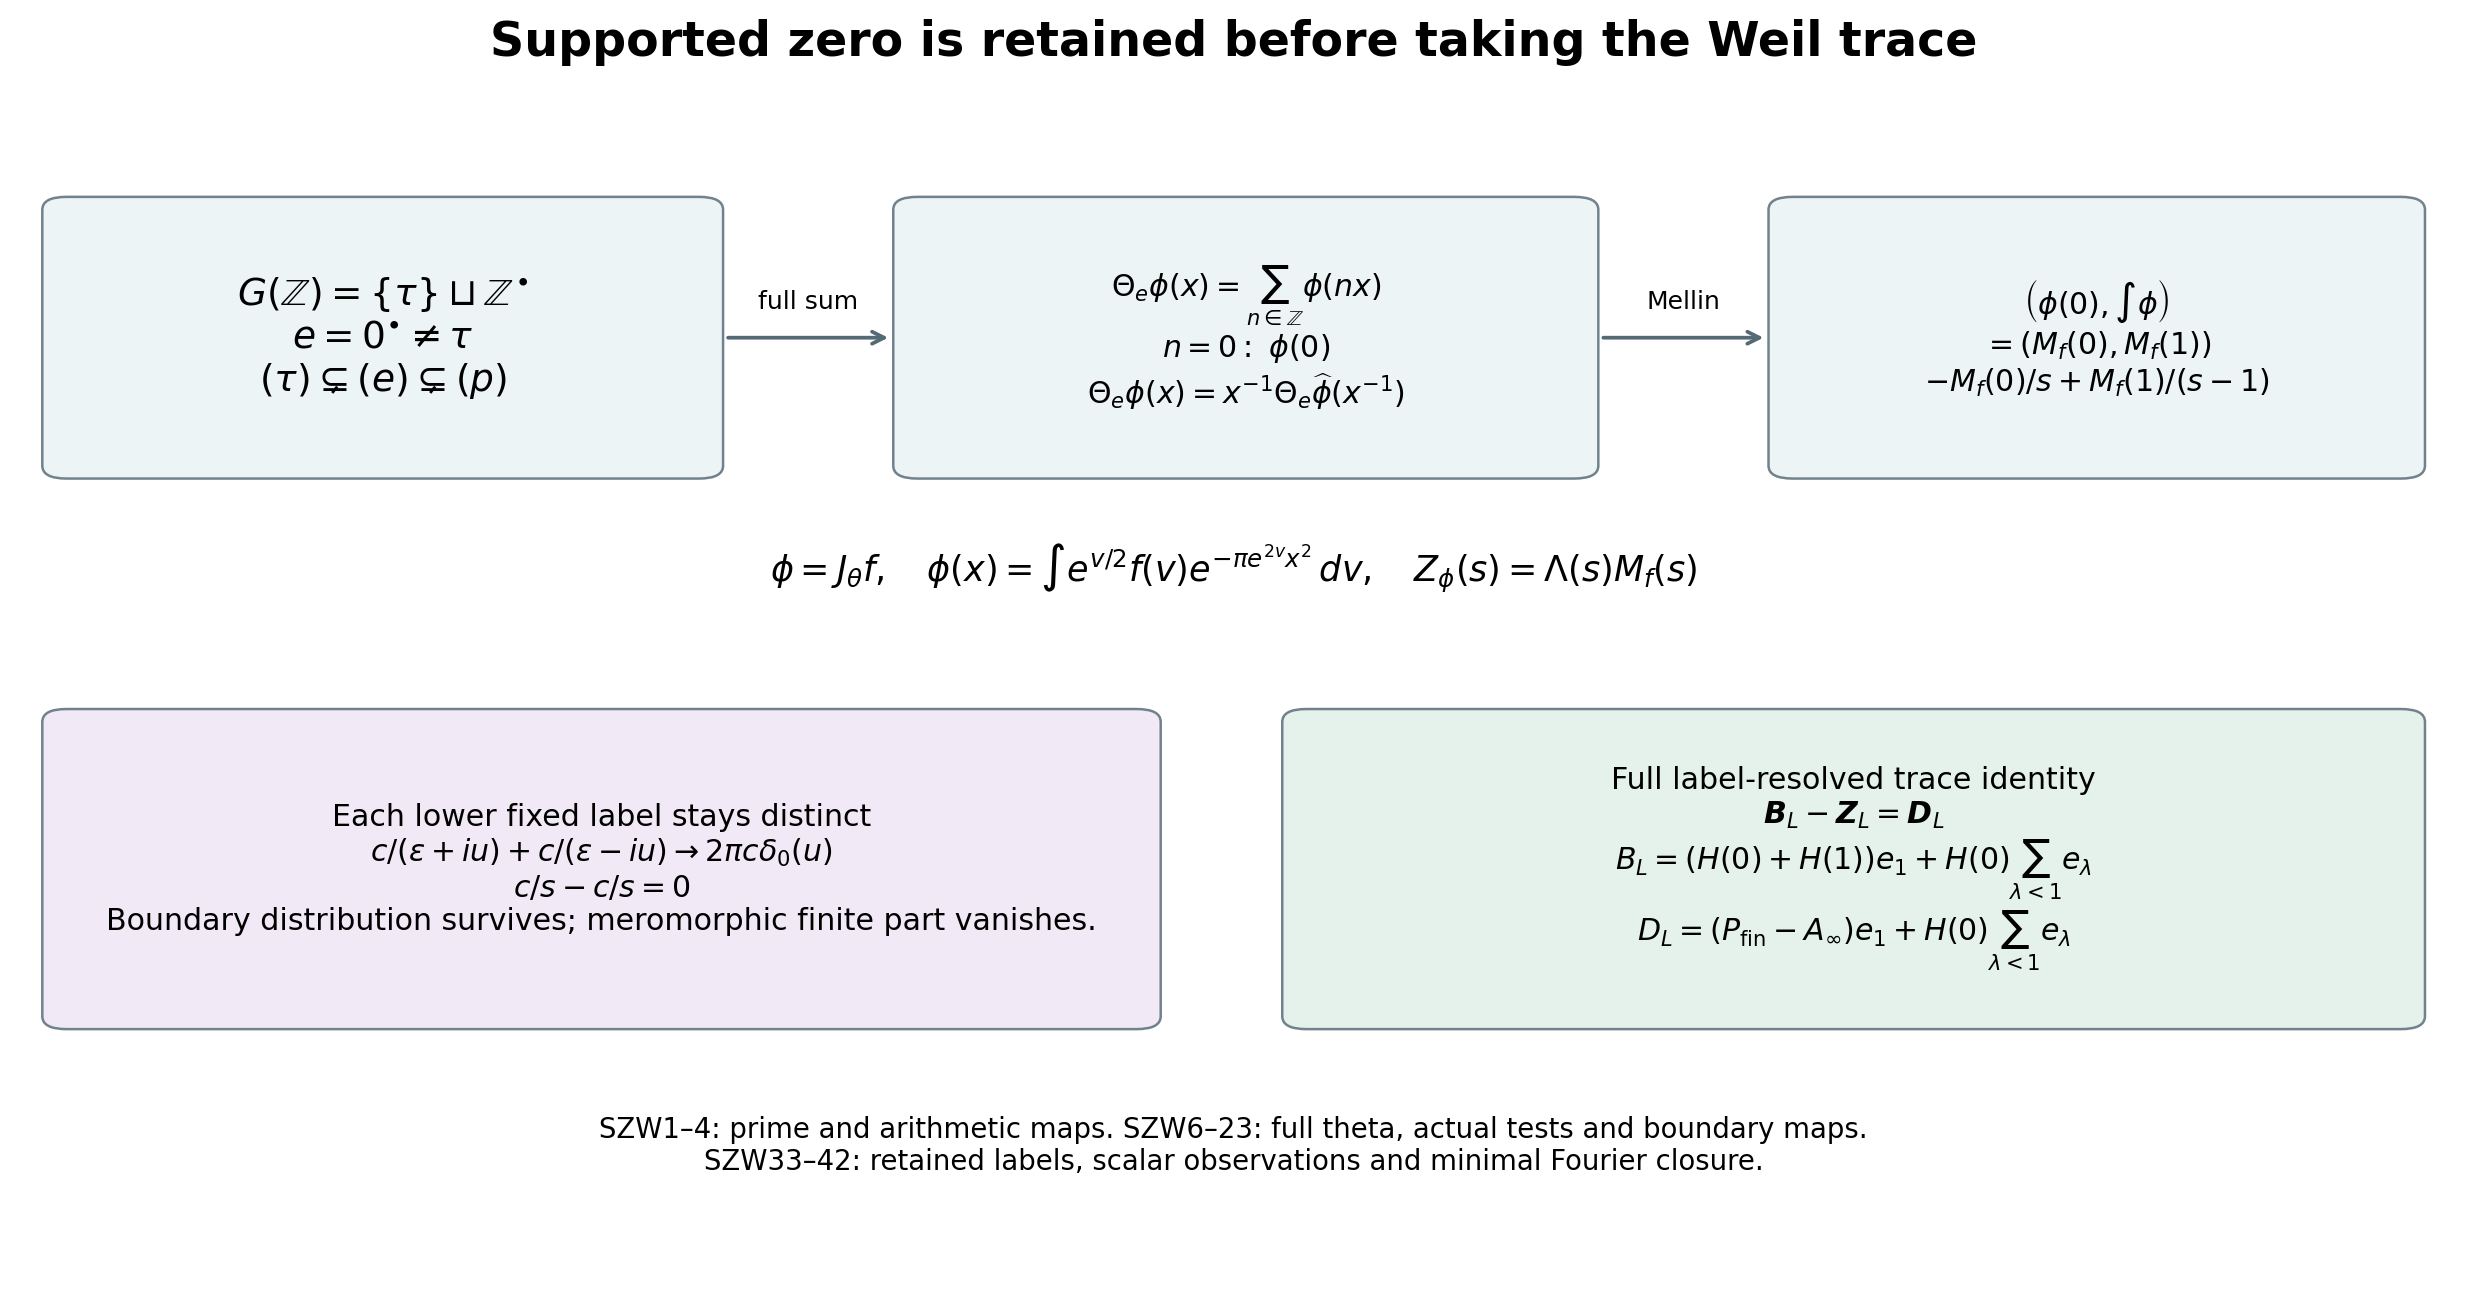
\includegraphics[keepaspectratio,alt={The actual supported-zero prime, its full theta and Mellin endpoint map, the retained fixed-support boundary distributions, and the full label-resolved trace identity. SZW1--SZW4, SZW6--SZW23 and SZW33--SZW42 prove the displayed maps and constants.}]{figures/32_supported_zero_weil.png}}
\caption{The actual supported-zero prime, its full theta and Mellin
endpoint map, the retained fixed-support boundary distributions, and the
full label-resolved trace identity. SZW1--SZW4, SZW6--SZW23 and
SZW33--SZW42 prove the displayed maps and constants.}
\end{figure}

\subsection{Exact residue-duality
continuation}\label{exact-residue-duality-continuation-1}

\href{COLLISION_RESIDUE_DUALITY_DERIVATION.md}{RD1--RD31b} proves the
complete Jacobian map from perfect residue duality to the retained
regular trace, identifies the actual packet radical with cotangent
cohomology, and computes the supported endpoint compensation. The
existing formulas and all their coordinates remain unchanged.

\subsection{Integral prism
continuation}\label{integral-prism-continuation}

\href{DISTINGUISHED_COLLISION_PRISM_DERIVATION.md}{DP1--DP43} constructs
the specific bounded prism and proves the original nilradical
specialization.
\href{NILRADICAL_COTANGENT_EXTENSION_CLASS_DERIVATION.md}{EC1--EC48}
computes its complete extension class and the exact maps detecting the
divided residue.
\href{SUPPORTED_PRISM_SPECTRUM_DERIVATION.md}{SG1--SG23} gives the
supported prime pullbacks, retaining the unsupported point and the
original supported-zero prime under coefficient contraction. These
calculations retain all earlier trace and endpoint identities.

\subsection{Actual global heat
continuation}\label{actual-global-heat-continuation}

The \href{ACTUAL_HEAT_ZERO_DISTRIBUTION_VARIATION.md}{global heat trace}
retains all zero multiplicities. The
\href{HEAT_CAUCHY_ARITHMETIC_DERIVATION.md}{arithmetic calculation,
HA1--HA26}, evaluates the complete supported formula on Cauchy tests and
computes its actual derivative. The local response keeps the complete
analytic unit; the global response includes mixed prime-product terms.
The \href{CAUCHY_WEIL_POSITIVITY_CRITERION.md}{matrix criterion} gives
the exact relation of this test family to RH. No sign from an isolated
local coefficient replaces the complete pairing.

\subsection{Exact full-form
continuation}\label{exact-full-form-continuation}

The \href{CAUCHY_REFLECTION_INDEX_DERIVATION.md}{reflection-index
theorem, NI1--32}, calculates the signed index of every complete Cauchy
coefficient tail. The
\href{FINITE_JET_COMPLEMENT_AND_HEAT_TRUNCATION.md}{finite-jet and
endpoint proof, FJ1--29}, preserves the exact finite jets while proving
density on the remaining zeros, derives the full exterior index and
tail, and calculates the second and third actual heat coefficients. All
supported endpoints remain explicit. These results identify the
remaining sign problem without asserting its resolution.

\subsection{One fixed primitive test and the entire prime
window}\label{one-fixed-primitive-test-and-the-entire-prime-window}

The \href{PRIME_PROJECTOR_MOBIUS_DERIVATION.md}{prime-operator
calculation}, PM1--41, proves both distinct Fourier support corrections
and their exact map into the full Weil formula. The
\href{PRIMITIVE_SHORT_SUPPORT_DERIVATION.md}{local estimate}, PS1--21,
gives a positive translation-difference remainder. The
\href{UNIVERSAL_PRIMITIVE_TRANSLATION_CRITERION.md}{fixed-test proof},
UP1--35, constructs one compact test whose transform is nonzero at every
possible off-critical zero. The
\href{PRIMITIVE_PRIME_WINDOW_DERIVATION.md}{complete arithmetic
calculation}, PW1--22, expresses its entire translated correlation
through a fixed-width prime window and an explicit archimedean
remainder. Its boundedness is equivalent to RH; that bound remains
unresolved. All boundary coordinates and supported-zero labels remain
explicit.

\clearpage

\section{Holonomy of the original signed eight-state
completion}\label{holonomy-of-the-original-signed-eight-state-completion}

23 September 2026. This derivation computes continuation of the actual
completed ES--Fable cover, including the omitted infinity sign, the two
original involutions, the complete finite trace forms, and the surviving
collision algebra. It distinguishes a permutation of nearby states from
an automorphism extending through a nonreduced fibre, and calculates the
residue when such an extension fails. No finite trace form in this note
is identified with an arithmetic Weil distribution.

Original sources read: the original finite signed-completion source
linked below, FS1--FS31, and
\href{https://github.com/KokunoYumeto/zeta-function-research-reader/blob/ab45e221579a0d48ce2885b4ecdf1a6aefc24a20/workbenches/splitzero-tandem/continuations/20260920-fable-boundary-action/FABLE_TO_ORIGINAL_CONDUCTOR.tex\#L2097}{\emph{The
ES--Fable inverse correspondence}, SM1--SM19, pinned original TeX,
source lines 2097--2513}, including the explicit paths and sign choices
in SM7--SM14. The latter already proves the order-192 monodromy group;
that result is not claimed as new here. The completed chart and local
algebra source is
\href{https://github.com/KokunoYumeto/zeta-function-research-reader/blob/0fd693c844aad9117e30ec447c59864a28af10f3/workbenches/splitzero-tandem/continuations/20260921-native-spectral-real-pair/005/independent/FINITE_SIGNED_COMPLETION.tex}{\emph{The
finite signed-root completion}, FS1--FS31, pinned original TeX}. Their
exact source hashes are, respectively,
\texttt{10906ba3\allowbreak{}bd21c066\allowbreak{}45571560\allowbreak{}e4c7b0c3\allowbreak{}948c0cca\allowbreak{}f65d8b9e\allowbreak{}525abf7c\allowbreak{}d732794c}
and
\texttt{eaf980a1\allowbreak{}6e7d639e\allowbreak{}21953e57\allowbreak{}79e7f76a\allowbreak{}bf18e8bd\allowbreak{}b80ae923\allowbreak{}c4160b45\allowbreak{}6c22da6f}.
The complete group proof needed here is included below. The receiving
heat calculation
\href{https://github.com/KokunoYumeto/zeta-function-research-reader/blob/d5c9d198a8432e3ede468b280162a99c00e3f4f7/workbenches/splitzero-tandem/branches/tau-zero-prime-positivity/EIGHT_STATE_HEAT_COMPARISON.md}{the
complete eight-state heat proof}, ESH1--ESH72, was read, and every used
map and local relation is restated and proved here. Source provenance of
the original polynomial is retained in FS's bibliography:
\emph{Erdős--Straus project reader}, source version 69,
\texttt{explicit-\allowbreak{}four-\allowbreak{}time-\allowbreak{}Jacobian-\allowbreak{}collision}; the added completion and
monodromy are programme derivations.

\subsection{1. The unchanged cover and its continuation
maps}\label{the-unchanged-cover-and-its-continuation-maps}

Retain target coordinates \(u=(A,B,C,D)\), the fixed cubic coefficient
one, and \[
\begin{aligned}
H_u(U,V)&=AU^4+U^3V+BU^2V^2+CUV^3+DV^4,\\
F_u(R)&=AR^4+R^3+BR^2+CR+D,\\
k_u(v)&=A+v+Bv^2+Cv^3+Dv^4.
\end{aligned}
\tag{EHM1}
\] The completed finite and infinity charts are \[
F_u(R)=0,\quad T^2=F'_u(R),\qquad
k_u(v)=0,\quad\Theta^2=-k'_u(v),
\quad v=R^{-1},\quad\Theta=-T/R.
\tag{EHM2}
\] The inverse transition is \(R=v^{-1},T=-\Theta/v\). At a root,
differentiation of \(k(v)=v^4F(1/v)\) gives \(k'(v)=-v^2F'(1/v)\),
proving both squared relations and every transition sign. Write
\(\mathfrak D\) for the binary quartic discriminant, with its original
value \(A^6\prod_{i<j}(R_j-R_i)^2\) when \(A\ne0\). The completed
unramified base is \[
\mathcal B^\circ=\{\mathfrak D\ne0\},\qquad
\mathcal B=\{A\mathfrak D\ne0\}\subset\mathcal B^\circ.
\tag{EHM3}
\] On \(\mathcal B^\circ\) each projective root is simple and has two
nonzero sign values. On a finite chart the relative Jacobian determinant
is \(2T F'(R)=2T^3\ne0\). At infinity, \(v=0\) forces \(A=0\) and
\(\Theta=\pm i\), and the relative determinant is
\(2\Theta k'(0)=2\Theta\ne0\). Thus these eight points have separate
local holomorphic inverse charts. Covering a compact path by finitely
many such neighborhoods and matching its initial point gives unique
continuation of each state. In particular infinity itself is not a
branch point of the completed cover.

For a finite root and nonzero \(T\), the original source coordinate
\(\alpha\), called \(a\) in FS, and the other three source coordinates
are \[
\begin{aligned}
\alpha&=T^{-1},\qquad y=-R-iT,\\
z&=AT^3+2RT+3iT^2,\\
w&=7iR^2T+(B-17R+AR^2)T^2-13iT^3-2AT^4.
\end{aligned}
\tag{EHM4}
\] These are FS13 in the unchanged reciprocal coordinate. They invert
the original factor equations:
\(b=-R/T,c=AT,d=(1+AR)T,e=(B+R+AR^2)T,f=(C+BR+R^2+AR^3)T\);
multiplication gives the four coefficients of EHM1, and the resultant is
\(T^{-2}F'(R)=1\). The original source is the completed cover with the
ramification divisor and the infinity sign \(\Theta=i\) removed. At
\(A=0\) its retained sign is \(\Theta=-i\), with source point
\((0,B,i(7B^2-C)/2,11B^3-2BC-D)\), as direct substitution in the
original polynomial verifies.

For a path entirely in \(\mathcal B\), order its roots continuously and
choose one initial \(T_j\) at each. The exact continuation formula is \[
T_j(t)=T_j(0)\exp\left(\frac12\int_0^t
\left[\frac{A'}A+\sum_{k\ne j}\frac{R'_j-R'_k}{R_j-R_k}\right]ds\right).
\tag{EHM5}
\] The denominators are nonzero on this path. Differentiating proves
that \(T_j^2/[A\prod_{k\ne j}(R_j-R_k)]\) is constant with value one.
The inverse source sign \(\alpha_j=1/T_j\) has the negative exponent,
exactly SM14. EHM2 supplies continuation through infinity where EHM5's
finite coordinates cannot be used.

\subsection{2. The original order-192 group, with its actual
generators}\label{the-original-order-192-group-with-its-actual-generators}

For four finite ordered roots let \(\Delta=\prod_{j<k}(R_k-R_j)\). The
derivative product is \(\prod_jF'(R_j)=A^4\Delta^2\): each of six
unordered pairs contributes a minus sign, whose product is one.
Therefore \[
\chi=A^2\Delta\prod_{j=1}^4\alpha_j,\qquad \chi^2=1.
\tag{EHM6}
\] This continuous value is constant along any ordered lift. A base loop
acts by \[
(j,\epsilon)\longmapsto(\pi(j),\sigma_j\epsilon),\qquad
\prod_j\sigma_j=\operatorname{sgn}(\pi),
\quad
G=\{(\sigma,\pi)\in\{\pm1\}^4\rtimes S_4:
\prod_j\sigma_j=\operatorname{sgn}(\pi)\}.
\tag{EHM7}
\] Indeed the final Vandermonde changes by \(\operatorname{sgn}(\pi)\),
while the product of source signs changes by \(\prod_j\sigma_j\), and
EHM6 fixes their product. The same signs describe \(T_j=1/\alpha_j\).
This gives \(|G|=8\cdot24=192\) as an upper bound.

The original SM7--SM11 realize the bound without assuming a braid-group
presentation. Retain their exact real roots, target, and inverse-source
signs: \[
\begin{gathered}
(R_1,R_2,R_3,R_4)=(7,9,11,13),\quad
u_{\mathrm{real}}=(-1/40,-59/4,95,-9009/40),\\
(\alpha_1,\alpha_2,\alpha_3,\alpha_4)
=(\sqrt{5/6},-i\sqrt{5/2},-\sqrt{5/2},i\sqrt{5/6}).
\end{gathered}
\tag{EHM8}
\] The derivatives are \((6/5,-2/5,2/5,-6/5)\), proving
\(\alpha_j^2F'(R_j)=1\) in each coordinate. For an adjacent pair, with
center \(c=(R_j+R_{j+1})/2\), take \[
R_j(\theta)=c-e^{i\theta},\quad
R_{j+1}(\theta)=c+e^{i\theta},\quad0\le\theta\le\pi,
\qquad \beta_j=(j+\ (j+1)+\ j-\ (j+1)-).
\tag{EHM9}
\] Keep the other roots and \(A=-1/40\) fixed. The root sum stays forty,
so the cubic coefficient stays one. The pair disk contains no other
root, and the endpoint unordered root set is the initial one, proving
this is a base loop. At a fixed root, the moving derivative factor is
\((R_k-c)^2-e^{2i\theta}\), contained in a right-half-plane disk not
meeting zero, so its logarithm has zero total change. At a moving root
the difference from its partner has argument change \(\pi\); each
difference from an outside root has a logarithm with zero imaginary
endpoint change, because it lies in a left or right half-plane and has
real endpoints of the same sign. Thus \(\alpha_j\) changes phase by
\(-\pi/2\). Substituting the four actual signs EHM8 proves exactly the
four-cycle EHM9 and fixes every other state.

The squares \(\beta_j^2\) flip the two adjacent signs. The three vectors
\((1,1,0,0),(0,1,1,0),(0,0,1,1)\) are independent over \(\mathbb F_2\)
and span the even-sum subspace, so these squares generate all eight
allowed pure sign patterns. The root permutations of the \(\beta_j\)
generate \(S_4\). The generated group therefore has at least
\(8\cdot24\) elements, proving that the upper bound EHM7 is attained.
Its product \(\beta_1\beta_2\beta_3\), applied rightmost first, is the
eight-cycle \((1+\ 2+\ 3+\ 4+\ 1-\ 2-\ 3-\ 4-)\). This is the
determinant-one signed-permutation group, not the even-sign group called
\(W(D_4)\): in the latter a signed four-cycle must have positive sign
product and order four, while all shorter-cycle combinations have order
dividing four or six, so no element has order eight.

The completed cover over \(\mathcal B^\circ\) has the same monodromy. At
a base point with \(A\ne0\), any loop in \(\mathcal B^\circ\) can be
moved slightly to avoid \(A=0\), with its base point fixed. Here is the
needed elementary justification. Cover the compact loop by finitely many
convex balls contained in \(\mathcal B^\circ\), subdivide its parameter,
and replace each piece by a polygon in these balls. Perturb the finitely
many vertices so that their \(A\)-coordinates are nonzero, and detour
any zero of a segment's linear \(A\)-coordinate by a small semicircle in
that complex coordinate, within the same ball. The replacements are
homotopic to the original paths inside these convex balls and avoid
\(A=0\). Thus every completed-loop permutation already occurs over
\(\mathcal B\). Conversely the loops EHM9 remain available, so the group
is exactly \(G\). The base is path connected: the discriminant
restricted to the complex line through any two allowed endpoints is a
nonzero polynomial, and detouring its finitely many zeros connects them.
Base-point changes therefore conjugate the permutation representation by
an actual bijection of path lifts. That bijection preserves each sign
pair, since the two initial opposite signs continue as opposites. The
determinant-one subgroup EHM7 is invariant under conjugation by such a
signed permutation, so the same description applies in the explicit
labels at \(u_*\).

\subsection{3. Labels and both involutions at the original seven-point
target}\label{labels-and-both-involutions-at-the-original-seven-point-target}

Use the original target \(u_*=(0,0,-1,0)\), with \(F_*(R)=R^3-R\). Label
all eight completed states by \[
\begin{array}{c|cccccccc}
\text{label}&a_+&a_-&b_+&b_-&c_+&c_-&m&n\\\hline
(R,T)\text{ or }(\infty,\Theta)&(1,\sqrt2)&(1,-\sqrt2)&(0,i)&(0,-i)&(-1,\sqrt2)&(-1,-\sqrt2)&(\infty,i)&(\infty,-i).
\end{array}
\tag{EHM10}
\] The missing original state is exactly \(m\). Write
\(\mathcal A_*\cong\mathbb C^8\) for the reduced fibre algebra, with
point idempotents \(e_x\). Evaluation supplies this isomorphism: the
root idempotents at \(0,1,-1\) are \(1-R^2,(R^2+R)/2,(R^2-R)/2\), and
splitting each nonzero sign quadratic gives its two indicator functions.
At infinity, \(e_m=(1-i\Theta)/2\) and \(e_n=(1+i\Theta)/2\), extended
by zero elsewhere. These formulas square to themselves, are
complementary, and evaluate to the indicated indicator values.

The original deck involution \(\Sigma\) negates \(T,\Theta\).
Coefficient conjugation \(\kappa\) fixes the coordinate generators.
Native \(J\) has target map \(j_{\mathrm{out}}(A,B,C,D)=(-A,-B,C,-D)\)
and chart maps \[
J(R,T)=(-R,-T),\qquad J(v,\Theta)=(-v,\Theta).
\tag{EHM11}
\] They follow either from EHM4 and
\(J(\alpha,y,z,w)=(-\alpha,-y,z,-w)\), or by substituting in
\(F_{j_{\mathrm{out}}u}(-R)=-F_u(R)\) and its derivative. At \(u_*\),
the relevant permutations on EHM10 are \[
\begin{aligned}
s&=(a_+a_-)(b_+b_-)(c_+c_-)(mn),\\
k&=(b_+b_-)(mn),\qquad
j=(a_+c_-)(a_-c_+)(b_+b_-),\\
\tau_\Sigma:=sk&=(a_+a_-)(c_+c_-),\qquad
\tau_J:=jk=(a_+c_-)(a_-c_+)(mn).
\end{aligned}
\tag{EHM12}
\] Here \(s,j\) act complex-linearly on the algebra; \(\kappa\),
\(\#_\Sigma=\Sigma\kappa\), and \(\#_J=J\kappa\) conjugate coefficients
as well as applying \(k,\tau_\Sigma,\tau_J\), respectively. Applying
their coordinate formulas to every state verifies EHM12, including the
fact that \(J\) fixes each infinity sign but \(\#_J\) exchanges them.

For any of these conjugate-linear involutions, the complete Hermitian
regular-trace pairing is \[
Q_\tau(f,g)=\sum_x\overline{f(\tau x)}g(x),\qquad
[Q_\tau]=P_\tau,
\tag{EHM13}
\] where \(P_\tau e_x=e_{\tau x}\). To prove it, multiplication by \(f\)
on the point basis is diagonal with entries \(f(x)\), so its trace is
their sum; now multiply \(\iota(f)g\). A fixed point of \(\tau\)
contributes one positive scalar form. A transposed pair contributes
\(\left(\begin{smallmatrix}0&1\\1&0\end{smallmatrix}\right)\), with one
positive and one negative eigenvalue. Hence the full inertias are \[
\operatorname{inertia}Q_k=(6,2,0),\quad
\operatorname{inertia}Q_{\tau_\Sigma}=(6,2,0),\quad
\operatorname{inertia}Q_{\tau_J}=(5,3,0).
\tag{EHM14}
\] In particular \(e_m\) is positive for \(Q_{\tau_\Sigma}\), but
isotropic for \(Q_{\tau_J}\), where it pairs with \(e_n\). The negative
native infinity vector is \(e_m-e_n\), with value \(-2\). The omitted
state, a negative direction, and a radical direction are therefore
explicitly related, but are not interchangeable names.

\subsection{4. An explicit loop involving the omitted infinity
state}\label{an-explicit-loop-involving-the-omitted-infinity-state}

The completed coefficient line \[
u(A)=(A,0,-1,0),\qquad
F_A(R)=R(AR^3+R^2-1),\qquad
\mathfrak D(u(A))=4-27A^2
\tag{EHM15}
\] starts at \(u_*\). The discriminant identity follows either from the
Sylvester determinant or from the cubic discriminant of \(AR^3+R^2-1\),
multiplied by the squared resultant with \(R\), which is one. Put
\(A_c=2/(3\sqrt3)\). For \(0<A<A_c\), the three nonzero roots consist of
\(R_L<-2/(3A)<R_C<0<R_P\): the cubic tends to minus infinity on the
left, has positive value \(4/(27A^2)-1\) at \(-2/(3A)\), value \(-1\) at
zero, and tends to plus infinity on the right. Its derivative has only
these two critical points, proving the stated root count and order. As
\(A\to0^+\), \(R_C\to-1,R_P\to1\), and \(R_L=-1/A+O(A)\), the original
infinity branch. At a nonzero root, \[
F_A'(R)=R^2(3AR+2),\qquad
\Theta^2=3AR+2.
\tag{EHM16}
\] The first follows by differentiating \(R(AR^3+R^2-1)\) at a root; the
second uses EHM2. For the stated large-root asymptotic, put \(w=AR_L\)
while \(A\ne0\); the root equation becomes \(w^2(w+1)=A^2\). Its
derivative in \(w\) at \((w,A)=(-1,0)\) is one, so its unique analytic
branch there satisfies \(w=-1+A^2+O(A^4)\), obtained by substituting its
convergent series. Dividing by the retained nonzero \(A\) gives
\(R_L=-1/A+A+O(A^3)\). EHM16 now gives \(\Theta\to\pm i\). Thus the sign
\(m\) continues along the large negative root with \(T=-R_L\Theta\)
positive imaginary, while \(c_+\) continues along \(R_C\) with positive
real \(T\).

At \(A_c\), the two negative roots collide at \(-\sqrt3\). The other
nonzero root is \(\sqrt3/2\). The collision is transverse because
\(\partial_A F_A(R)=R^4=9\) and \(\partial_R^2F_A(R)=2\sqrt3\ne0\)
there. Choose a sufficiently small \(\epsilon>0\), approach
\(A_c-\epsilon\) along the positive real interval, traverse the circle
\(A=A_c+\epsilon e^{i\theta}\), \(\pi\le\theta\le3\pi\), and return
along the interval. No other discriminant point lies on or within this
small disk. The resulting based-loop permutation is \[
g_\infty=(m\ c_-\ n\ c_+),\qquad
g_\infty^2=(mn)(c_+c_-),
\tag{EHM17}
\] fixing \(a_\pm,b_\pm\). Here is the sign computation. In the local
coordinate centered at the collision, the two root displacements
initially are negative and positive real; their difference makes a
positive half-turn as the target makes one turn. The derivative at the
negative displacement initially is negative real and at the positive
displacement positive real, since \(F_{RR}>0\). Each derivative
therefore acquires argument change \(\pi\); its square root acquires
phase \(i\). Thus positive imaginary \(T\) on the large branch ends as
negative real \(T\) on the other branch, giving \(m\mapsto c_-\),
whereas positive real \(T\) on that branch ends as positive imaginary on
the large branch, giving \(c_+\mapsto m\). Negating signs gives the
other two arrows. Analytic nonzero factors have logarithms on this small
disk and contribute no further winding. The other two root pairs have
separate holomorphic nonzero sign branches and are fixed. Returning
along the real interval proves the exact labels in EHM17.

This loop leaves \(A=0\); loops entirely in its simple-root locus fix
the two infinity sections \(\Theta=\pm i\). The missing infinity state
is nevertheless in the full monodromy orbit. In particular, two
traversals take the retained state \(n\) to the omitted state \(m\). On
its returning original affine inverse branch, \(T=-iR_L(1+O(A^2))\), so
EHM4 gives \[
y=-2R_L+O(A)=2/A+O(A),\qquad\alpha=1/T\longrightarrow0.
\tag{EHM18}
\] Thus the loop has a bounded lift in the completed cover and an
escaping lift at the endpoint in the original affine chart. This is the
actual relation of the nontrivial holonomy to the seventh/eighth
distinction, with its original coordinate divergence.

Let \(v_c=e_{c_+}-e_{c_-}\) and \(v_\infty=e_m-e_n\). Under the
point-permutation action \(\rho(g)e_x=e_{gx}\), \[
\rho(g_\infty)v_c=v_\infty,\qquad
\rho(g_\infty)v_\infty=-v_c,
\qquad Q_{\tau_\Sigma}(v_c,v_c)=-2,
\quad Q_{\tau_\Sigma}(v_\infty,v_\infty)=2.
\tag{EHM19}
\] All four equations follow by applying EHM17 and EHM12. One negative
and one positive direction are exchanged. Both remain in the same
eight-dimensional space; the next section calculates exactly what
happens to the form.

\subsection{5. The typed transport of the forms and
involutions}\label{the-typed-transport-of-the-forms-and-involutions}

The action \(\rho(g)e_x=e_{gx}\) is a unital algebra automorphism of
\(\mathbb C^8\), because it permutes the orthogonal primitive
idempotents. It preserves the complex bilinear regular trace pairing and
the positive coefficient form \(\sum_x\overline{f(x)}g(x)\). For an
original conjugate-linear involution with point permutation \(\tau\),
exact substitution gives \[
Q_\tau(\rho(g)f,\rho(g)h)=Q_{g^{-1}\tau g}(f,h),\qquad
\rho(g)\iota_\tau\rho(g)^{-1}=\iota_{g\tau g^{-1}}.
\tag{EHM20}
\] Thus \(\rho(g)\) is an isometry from \(Q_\tau\) to
\(Q_{g\tau g^{-1}}\). It preserves the original fixed form precisely
when \(g\tau=\tau g\), since equality of the matrices in EHM13 is then
necessary and sufficient. EHM19 does not meet that condition; it is not
a sign flip by an isometry of the unchanged indefinite form.

The same fact has a pathwise formulation retaining both native maps.
Uniqueness of lifts gives \[
\Sigma M_\gamma=M_\gamma\Sigma,\qquad
\kappa M_\gamma\kappa=M_{\overline\gamma},\qquad
J M_\gamma J^{-1}=M_{j_{\mathrm{out}}\gamma}.
\tag{EHM21}
\] For a path with differing endpoints these are identities between its
stated endpoint fibres; at the real, native-fixed base point \(u_*\)
they are identities on that fibre. Conjugating a lifted path by the
respective coordinate map gives a lift of the transformed base path with
the corresponding initial point, which proves each equality. Combining
the second identity with the first or third gives the corresponding
equations for \(\#_\Sigma\) and \(\#_J\). In particular native
reflection of \(\gamma_+(h)=(0,0,-1-16h,16h)\) is
\(\gamma_-(h)=(0,0,-1-16h,-16h)\), generally a different target path.
Native reflection is not to be substituted for continuation around a
loop of \(\gamma_+\).

The seven-state quotient has its exact transported family. For any state
\(x\), let \(q_x:\mathcal A_*\to\mathcal A_*/\mathbb Ce_x\). Then \[
\overline\rho_g:\mathcal A_*/\mathbb Ce_x\xrightarrow{\sim}
\mathcal A_*/\mathbb Ce_{gx},\qquad
\overline\rho_g q_x=q_{gx}\rho(g).
\tag{EHM22}
\] This is well defined because
\(\rho(g)(\mathbb Ce_x)=\mathbb Ce_{gx}\); its inverse is induced by
\(g^{-1}\). Since \(G\) is transitive, the smallest monodromy-stable
ideal containing the omitted line \(\mathbb Ce_m\) is all of
\(\mathcal A_*\): it contains every point idempotent and hence their sum
one. Consequently there is no nonzero quotient algebra with the full
induced monodromy action that kills exactly this one state. The
seven-state objects instead form the explicitly transported family
EHM22, or a single such quotient over its stabilizer subgroup of order
\(192/8=24\). This proves the obstruction and its replacement object,
rather than treating the missing state as unrelated to the cover.

\subsection{6. Both meridians of the actual chosen heat
path}\label{both-meridians-of-the-actual-chosen-heat-path}

Retain \[
\gamma_+(h)=(0,0,-1-16h,16h),\qquad
F_h(R)=(R-1)(R^2+R-16h),\qquad
\operatorname{Disc}F_h=(2-16h)^2(1+64h).
\tag{EHM23}
\] The factorization follows by expansion. For the discriminant, the
quadratic discriminant is \(1+64h\), and its resultant with \(R-1\) is
its value \(2-16h\) at one; the product of squared pairwise root
differences gives their stated product. Thus the path meets the
discriminant at \(h_c=1/8\) with multiplicity two and at \(h_d=-1/64\)
with multiplicity one. On the branch \(s(h)=\sqrt{1+64h}\) with
\(s(0)=1\), its roots and derivatives are \[
R_a=1,\quad R_b=(-1+s)/2,\quad R_c=(-1-s)/2,
\qquad
\mu_a=(9-s^2)/4,\quad\mu_b=s(s-3)/2,\quad\mu_c=s(s+3)/2.
\tag{EHM24}
\] The derivatives follow by evaluating \(3R^2-1-16h\), or by
differentiating the factorization at each root.

Take the positive meridian around \(h_c\) approached along \((0,h_c)\),
and the positive meridian around \(h_d\) approached along \((h_d,0)\).
In the exact base labels EHM10 their permutations are \[
g_c=(a_+a_-)(b_+b_-),\qquad
g_d=(b_+\ c_-\ b_-\ c_+).
\tag{EHM25}
\] Near \(h_c\), all three root functions are individually holomorphic,
\(\mu_a,\mu_b\) have simple zeros, and \(\mu_c\) has none. The first two
square roots therefore change sign once, and the third does not, proving
the first formula. Around \(h_d\), let \(h=h_d+\epsilon e^{i\theta}\),
starting to its right; then \(s=8\sqrt\epsilon e^{i\theta/2}\) makes an
upper half-circle. For sufficiently small \(\epsilon\), the continuous
argument of \(\mu_b\) runs from \(\pi\) to \(2\pi\), and that of
\(\mu_c\) from zero to \(\pi\): in EHM24 the factors \(s-3,s+3\) remain
in their respective left and right half-planes, with real endpoint
ratios of the same sign. Consequently \(b_+\mapsto c_-\),
\(c_+\mapsto b_+\), and the other two arrows follow by negating signs.
This proves the second formula. The infinity states are the constant
sections \(\Theta=\pm i\) on this path and are fixed by both loops.

These permutations obey \(g_c^2=1,g_d^4=1,g_cg_dg_c=g_d^{-1}\). The four
powers of \(g_d\) fix \(a_\pm\), and the four elements \(g_cg_d^j\)
exchange them, so these eight elements are distinct; the relations
reduce every word to one of them. The path's monodromy is thus the group
of order eight \[
\langle g_c,g_d\rangle\cong D_8,
\qquad g_d^2=(b_+b_-)(c_+c_-).
\tag{EHM26}
\] The base is the complex \(h\)-plane with these two points deleted. To
see that these two meridians generate all its loop permutations,
surround each puncture by a small disjoint disk and join their
boundaries to the base point by nonintersecting arcs. Cutting a large
disk containing any given compact loop along those arcs leaves a region
without holes, in which the loop reduces to successive boundary
traversals of the two punctures. These are the two stated meridians and
their inverses. This supplies the elementary topological generation
needed for the equality, rather than only a subgroup assertion.

The first loop is an isometry of the fixed \(Q_{\tau_\Sigma}\), since
both permutations in EHM12 and \(g_c\) are products of individual pair
flips. It sends the negative vector \(v_a=e_{a_+}-e_{a_-}\) to \(-v_a\)
and the positive vector \(v_b=e_{b_+}-e_{b_-}\) to \(-v_b\); their
squared values stay \(-2\) and \(2\). The second loop instead sends
\(v_c\mapsto v_b\) and \(v_b\mapsto-v_c\), exchanging values \(-2\) and
\(2\) for the fixed form. Its transported form is exactly EHM20.
Therefore neither nontrivial continuation nor a sign change alone proves
positivity of the unchanged pairing.

\subsection{7. The exact local family, the retained radical, and the
regular heat-loop
extension}\label{the-exact-local-family-the-retained-radical-and-the-regular-heat-loop-extension}

Put \(t=h-1/8\), \(\epsilon=R-1\), and \[
\beta(t)=\frac{\sqrt{9+64t}-3}{2},\quad\beta(\beta+3)=16t,
\qquad
\mathscr L=\frac{\mathbb C\{t\}[\epsilon,T]}
{(\epsilon^2-\beta\epsilon,\ T^2+16t-(6+3\beta)\epsilon)}.
\tag{EHM27}
\] Here \(\mathbb C\{t\}\) means convergent power series at zero and the
square root has value three. The root branches in this cluster are
\(\epsilon=0,\beta\); the third root is separated, so its root factor is
invertible in this local algebra. Reducing
\(F_h'(1+\epsilon)=6\epsilon+3\epsilon^2-16t\) by
\(\epsilon^2=\beta\epsilon\) proves the second relation. Successive
division by the two monic relations proves that
\(1,\epsilon,T,\epsilon T\) is a free basis. The special fibre is
therefore \[
\mathscr L_0=\mathbb C[\epsilon,T]/(\epsilon^2,T^2-6\epsilon)
\cong\mathbb C[T]/(T^4),\qquad\epsilon=T^2/6.
\tag{EHM28}
\] Substitution proves both inverse maps in this isomorphism.

The chosen-loop permutation \(g_c\) has the regular local-family
realization \(\epsilon\mapsto\epsilon,T\mapsto-T\). On the whole
eight-state family near \(h_c\), let \[
e_c(h,R)=\frac{(R-1)(R-R_b(h))}{(R_c(h)-1)(R_c(h)-R_b(h))},
\qquad R\mapsto R,\quad T\mapsto(2e_c-1)T,\quad\Theta\mapsto\Theta.
\tag{EHM29}
\] The denominator stays nonzero near \(h_c\). The numerator evaluates
to zero on the cluster and to its denominator at the separated root, so
it is the separated-root idempotent. Since \((2e_c-1)^2=1\), this map
preserves the entire signed relation, flips just the two cluster signs,
and fixes the separated pair and infinity states. It is an involution
and realizes EHM25. At \(h_c\), \(e_c=(R-1)^2/9\). This is a local
extension of this loop, not the global sign deck map, which would negate
all eight signs.

Retain the original radical generators, extended by zero on the
separated and infinity factors: \[
\begin{aligned}
n_1&=(R-1)(R+2)=T^2/2,\\
n_2&=T(R+2)=3T+T^3/6,\\
n_3&=T(R-1)(R+2)=T^3/2.
\end{aligned}
\tag{EHM30}
\] The right sides follow from \(R=1+T^2/6\) modulo \(T^4\). Conversely
\(T=n_2/3-n_3/9,T^2=2n_1,T^3=2n_3\), proving independence and spanning
of \(\mathfrak N=(T)\). Multiplication gives \[
n_2^2=18n_1,\quad n_1n_2=3n_3,\quad
n_1^2=n_1n_3=n_2n_3=n_3^2=0,
\quad\mathfrak N^2=\langle n_1,n_3\rangle,\quad
\mathfrak N^3=\langle n_3\rangle,\quad\mathfrak N^4=0.
\tag{EHM31}
\] Each assertion follows by multiplying the displayed powers of \(T\);
the nonzero products and independence prove the stated ideal powers. The
specialized loop acts by \[
g_c^*: (n_1,n_2,n_3)\longmapsto(n_1,-n_2,-n_3).
\tag{EHM32}
\] Here the point map and its pullback are both involutions, so the
idempotent-transport convention \(\rho\) agrees with the pullback in
this case.

Every \(f\in\mathscr L_0\) has multiplication trace \(4f(0)\): its
nonconstant part lies in the nilpotent ideal and has a nilpotent
multiplication operator, while its constant part acts on four basis
vectors. The conjugate-deck form, with \(T^\#=-T\), is consequently \[
Q_{\mathscr L_0}(f,g)=4\overline{f(0)}g(0),\qquad
\operatorname{rad}Q_{\mathscr L_0}=\mathfrak N.
\tag{EHM33}
\] The complete special fibre is
\(\mathscr L_0\times\mathbb C[T_c]/(T_c^2-9)\times\mathbb C[\Theta]/(\Theta^2+1)\).
Its latter forms have Gram matrices \(\operatorname{diag}(2,-18)\) and
\(\operatorname{diag}(2,2)\); direct multiplication proves them as in
EHM13. Thus the whole form has inertia \((4,1,3)\), and the nonzero
negative separated vector remains. The local radical is exactly the
kernel of the regular trace pairing, not an assertion that its elements
vanish as algebra elements.

The original HEB map is the further quotient setting \(R=1\), hence
\(T^2=0\), with \(r_H=T/(2\sqrt2)\). Its exact sequence on the radical
is \[
0\longrightarrow\mathfrak N^2\longrightarrow\mathfrak N
\xrightarrow{\pi_1}\mathbb Cr_H\longrightarrow0,
\quad\pi_1(n_1)=0,\quad\pi_1(n_2)=6\sqrt2\,r_H,\quad\pi_1(n_3)=0.
\tag{EHM34}
\] These images follow by evaluation in EHM30, proving the kernel,
surjectivity, and constants. The loop \(g_c\) negates this surviving
infinitesimal and preserves its nonzero algebra class.

\subsection{8. The transverse order-four collision and its
original-coordinate
correction}\label{the-transverse-order-four-collision-and-its-original-coordinate-correction}

An actual transverse path through the same coefficient point is \[
F_z(R)=((R-1)^2-z)(R+2),\quad
u(z)=(0,0,-3-z,2-2z),\quad
x=R-1,\quad x^2=z,\quad T^2=2x(x+3).
\tag{EHM35}
\] Expansion proves the target formula, and differentiating on the root
relation proves the last equation. Choose the analytic square root
\(g(x)=\sqrt{2(x+3)}\) with \(g(0)=\sqrt6\). Then \[
y=T/g(x),\quad y^2=x,\quad y^4=z,
\qquad x=y^2,\quad T=yg(y^2).
\tag{EHM36}
\] Both compositions are exact and analytic near the local point because
\(g\) never vanishes. Positive point continuation is \(y\mapsto iy\).
Its analytic deck map and coordinate pullback are \[
\alpha:(x,T)\longmapsto\left(-x,,iT\sqrt{\frac{3-x}{3+x}}\right),
\qquad \alpha^2:(x,T)\longmapsto(x,-T).
\tag{EHM37}
\] The ratio is the specific analytic branch with value one at zero.
Substitution in EHM36 proves the equations and the square, without
omitting any unit factor. At the special fibre, using \(x=T^2/6,x^2=0\),
its pullback is \[
\alpha_0^*(T)=iT-\frac{i}{18}T^3,\qquad
\alpha_0^*(n_1)=-n_1,\quad
\alpha_0^*(n_2)=in_2-in_3,\quad
\alpha_0^*(n_3)=-in_3.
\tag{EHM38}
\] Indeed \(\sqrt{(3-x)/(3+x)}=1-x/3\) modulo \(x^2\), giving the first
formula. Inserting it in EHM30 gives the remaining three. Its square
sends \(T\) to \(-T\) and its fourth power is the identity. Thus it
preserves all products EHM31. The correction \(-iT^3/18\) is required
for the analytic continuation in the original reciprocal coordinate.

The distinction between point maps and pullbacks is explicit: a point
map \(\alpha\) has pullback \(\alpha^*e_x=e_{\alpha^{-1}x}\). Therefore
the forward idempotent transport \(\rho(\alpha)e_x=e_{\alpha x}\) of
EHM20 is \((\alpha^{-1})^*\). On this special local algebra it sends
\(T\mapsto-iT+iT^3/18\), with the inverse of the three radical
transformations EHM38. Both maps have the same invariants and
coinvariants, but opposite eigenvalues \(i,-i\) on the corresponding
nonreal eigenspaces. This retains the orientation rather than silently
changing the convention for a four-cycle.

The relation with the chosen heat path is itself an exact map. Put \[
m(t)=(1+R_b)/2,\quad d(t)=(1-R_b)/2,
\quad\ell(t)=m(t)-R_c,\quad x=R-m(t).
\tag{EHM39}
\] Then \(F_h(R)=(x^2-d(t)^2)(x+\ell(t))\) by its three root factors.
Also \[
d(t)=-\frac{16t}{3+\sqrt{9+64t}},\qquad
d(t)^2=\frac{256t^2}{(3+\sqrt{9+64t})^2}.
\tag{EHM40}
\] These identities follow by rationalizing \((3-\sqrt{9+64t})/4\). The
denominator is an analytic nonzero unit near zero, so one small positive
\(t\)-loop makes this transverse parameter wind twice. Replacing \(x+3\)
in EHM36 by the retained analytic unit \(x+\ell(t)\) gives the same
exact fourth-root calculation. Its continuation is consequently the
square of the transverse order-four map, exactly \(g_c\). This proves
the relationship between the two paths and their cycle orders.

At the other collision put \(v=h+1/64,x=R+1/2\). Direct expansion gives
\(F_h=(x^2-16v)(x-3/2)\) and \(T^2=2x(x-3/2)\) on the root algebra.
Choosing \(\sqrt{2(x-3/2)}\) with value \(i\sqrt3\) gives the exact
coordinate \(y=T/\sqrt{2(x-3/2)}\) with \(y^4=16v\). At the special
fibre \(x=-T^2/3\), so its positive point continuation has pullback \[
\alpha_{d,0}^*(T)=iT-\frac{2i}{9}T^3,\qquad
(\alpha_{d,0}^*)^2(T)=-T.
\tag{EHM41}
\] This follows by expanding the corresponding ratio square root to
first order in \(x\). Its branch has the four-cycle \(g_d\) from EHM25.
It is a regular specialization at its own collision, which does not
imply regular specialization at the different collision \(h_c\).

\subsection{9. The regular-extension obstruction and its nonzero
residue}\label{the-regular-extension-obstruction-and-its-nonzero-residue}

A based permutation is not automatically a single-valued deck map over
the punctured \(h_c\)-disk. Such a deck map must commute with the local
monodromy \(g_c\): apply it before and after lifting a local loop and
use uniqueness. Conversely a commuting permutation extends uniquely over
that punctured disk by continuing it in the eight local branches;
commutation makes the result independent of the chosen continuation
path. Inside the explicitly computed \(D_8\), the centralizer is \[
C_{D_8}(g_c)=\{1,g_c,g_d^2,g_cg_d^2\}.
\tag{EHM42}
\] Indeed \(g_cg_d^j=g_d^{-j}g_c\), so commutation requires
\(g_d^j=g_d^{-j}\), exactly even \(j\); multiplying by \(g_c\) gives the
other two. Thus the odd powers of \(g_d\), and their \(g_c\)-multiples,
already require a slit neighborhood to label their transported maps.
They also move some states in the four-point collision cluster to
separated reduced states. Any holomorphic extension to the special fibre
would preserve its unique nonreduced local factor, so these maps could
not extend through the collision even after attempting that
identification.

The commuting element \(g_d^2\) has a stronger, explicitly calculable
obstruction. It fixes the \(a\)-sign and flips only the \(b\)-sign in
the local cluster. The two local root values of \(\epsilon\) are zero
and \(\beta\), so its unique generic algebra formula is \[
S_b(\epsilon)=\epsilon,\qquad
S_b(T)=\left(1-\frac{2\epsilon}{\beta}\right)T,
\qquad S_b(\epsilon T)=-\epsilon T.
\tag{EHM43}
\] The interpolation multiplier has values one and minus one on the two
root branches. Its square is one because \(\epsilon^2=\beta\epsilon\),
proving that this is an involutive algebra automorphism on the punctured
disk; the last equation follows from that same relation. This is its
only possible continuation there, since the eight reduced points
determine the algebra map. The separated \(c\)-factor also changes sign
under \(g_d^2\), but this is a bounded, regular operation on that
separate factor.

The simple zero of \(\beta\) produces an actual pole in the free basis
EHM27. Its residue, meaning the specialization of the operator \(tS_b\)
at \(t=0\), is \[
\begin{aligned}
\left.tS_b(T)\right|_{0}
&=-\left.\frac{2t}{\beta}\epsilon T\right|_0
=-\frac38\epsilon T=-\frac{T^3}{16}\ne0,\\
\left.tS_b(1)\right|_0&=\left.tS_b(\epsilon)\right|_0
=\left.tS_b(\epsilon T)\right|_0=0.
\end{aligned}
\tag{EHM44}
\] Here \(t/\beta=(\beta+3)/16\) follows from EHM27, and
\(\epsilon T=T^3/6\) at the collision. Freeness of the four-element
basis shows that this nonzero pole cannot be removed by another regular
formula agreeing on the punctured disk. Projection onto the analytic
cluster summand shows that adjoining the separated and infinity factors
cannot cancel it either.

The residue is exactly the derivation \[
\delta=-\frac{T^3}{16}\frac{d}{dT}:
\mathbb C[T]/(T^4)\longrightarrow\mathbb C[T]/(T^4),
\qquad
\ker\delta=\mathbb C1\oplus(T^2),\quad
\operatorname{im}\delta=(T^3),\quad\delta^2=0.
\tag{EHM45}
\] The polynomial derivation preserves the ideal \((T^4)\), since it
sends \(T^4\) to \(-T^6/4\); hence it descends and obeys the Leibniz
identity. On \(1,T,T^2,T^3\), its values are \(0,-T^3/16,0,0\), exactly
EHM44. These four values prove the kernel, image, and square. In the
retained radical coordinates this is \[
\delta(n_1)=0,\qquad\delta(n_2)=-\frac38n_3,
\qquad\delta(n_3)=0,
\qquad
\overline\delta:\mathfrak N/\mathfrak N^2\xrightarrow{\sim}\mathfrak N^3,
\quad[n_2]\longmapsto-\frac38n_3.
\tag{EHM46}
\] The values follow by applying EHM45 to EHM30. Since \(\delta\) kills
\(\mathfrak N^2\), the quotient map is well defined; both its source and
target are one dimensional and its displayed value is nonzero, proving
the isomorphism. This residue is an actual nonzero map between the
retained infinitesimal layers. Its value depends on the specified
original clock \(t=h-1/8\), whose scale is kept in EHM44.

The other nontrivial commuting candidate \(g_cg_d^2\) acts on \(T\) by
the negative of EHM43 and has residue \(-\delta\). Consequently exactly
\[
\{1,g_c\}\subset\langle g_c,g_d\rangle
\tag{EHM47}
\] extends holomorphically over the whole \(h_c\)-fiber. These two
extensions were constructed in EHM29. All others fail either the
punctured-disk commutation condition or the explicit nonzero residue
test. This is a complete classification within the actual based
heat-path group, not a claim that the different transverse local group
has only two extending elements: its four elements were explicitly
constructed in EHM37.

\subsection{10. The action on invariants, coinvariants, and the trace
radical}\label{the-action-on-invariants-coinvariants-and-the-trace-radical}

For any finite permutation group \(K\) acting on the eight states, let
\(V=\mathbb C^8\), \(V^K\) be its invariant vectors, and \(V_K=V/W_K\),
where \(W_K=\operatorname{span}\{\rho(g)v-v:g\in K,v\in V\}\). For an
orbit \(O\) let \(u_O=\sum_{x\in O}e_x\). The exact maps are \[
\mathcal P_Kv=\sum_{O}\frac{\sum_{x\in O}v_x}{|O|}u_O,
\qquad
0\longrightarrow W_K\longrightarrow V\xrightarrow{\mathcal P_K}V^K\longrightarrow0,
\qquad V_K\xrightarrow{\sim}V^K,\quad[v]\mapsto\mathcal P_Kv.
\tag{EHM48}
\] On every orbit the differences \(e_x-e_y\) span the
coefficient-sum-zero subspace: choose one base point in the orbit and
subtract it from all the others. Each such difference belongs to \(W_K\)
because some group element takes one point to the other. Hence \(W_K\)
is exactly the direct sum of those subspaces, proving the kernel,
exactness, and quotient isomorphism. The invariant algebra consists of
functions constant on each orbit and is
\(\mathbb C^{\#\mathrm{orbits}}\), with trace weights \(|O|\). The map
\(\mathcal P_K\) is linear and is not in general multiplicative: for two
different points in a nontrivial orbit, their product is zero, whereas
the product of their two images is \(u_O/|O|^2\ne0\). Thus the linear
coinvariant space has not been assigned an unjustified quotient-algebra
product. The ideal generated by the differences kills every nontrivial
orbit, since multiplying \(e_x-e_y\) by \(e_x\) gives \(e_x\).

The actual dimensions and restrictions of the unchanged conjugate-deck
form are \[
\begin{array}{c|c|c|c}
K&\text{nontrivial state orbits}&\dim V^K=\dim V_K&
\operatorname{inertia}(Q_{\tau_\Sigma}|_{V^K})\\\hline
\langle g_c\rangle&\{a_+,a_-\},\{b_+,b_-\}&6&(5,1,0)\\
\langle g_d\rangle&\{b_+,c_-,b_-,c_+\}&5&(4,1,0)\\
\langle g_c,g_d\rangle&\{a_+,a_-\},\{b_+,b_-,c_+,c_-\}&4&(4,0,0)\\
G&\text{all eight states}&1&(1,0,0).
\end{array}
\tag{EHM49}
\] To prove the signature entries without a dimension inference, every
displayed orbit sum has positive value equal to its cardinality, since
its orbit is preserved by \(\tau_\Sigma\). For the first row the
remaining \(c_+,c_-\) block is hyperbolic and the two infinity states
are positive. For the second the remaining \(a_+,a_-\) block is
hyperbolic and infinity is positive. In the last two rows every
invariant basis vector is an orbit sum and these sums have disjoint
supports, giving mutually orthogonal positive values. These are
restrictions to explicitly mapped subspaces, not positivity of the full
original form. On the reduced eight-state fibre none of these nontrivial
linear coinvariant projections makes the original full form descend by
arbitrary lifts: its radical is zero by EHM14, whereas \(W_K\ne0\). A
form descends through a projection precisely when its kernel pairs to
zero with every vector, which proves this obstruction directly. The
projection EHM48 still supplies its specified comparison with the
invariant restriction.

At the nonreduced collision, the answer changes in an exactly calculable
way. The extending local heat involution has invariants
\(\langle1,T^2\rangle\) and difference space \(\langle T,T^3\rangle\).
The latter lies in the trace radical \((T)\), so the local form EHM33
does descend to its two-dimensional linear coinvariant space, with
radical the surviving class of \(T^2\). Its invariant restriction has
inertia \((1,0,1)\). On the whole fibre the unchanged separated factor
and infinity pair add their signatures, giving the complete
invariant/coinvariant form inertia \[
(4,1,1)\quad\text{for the extending heat involution at }h_c.
\tag{EHM50}
\] By contrast, the transverse order-four map EHM38 has eigenvalues
\(1,i,-1,-i\) on a suitable basis of \(\mathscr L_0\). One may use the
exact coordinate \(y=T/\sqrt{2(3+T^2/6)}\) from EHM36, in which the
basis \(1,y,y^2,y^3\) gives these four values; its linear change of
basis is invertible since the coefficient of \(T\) in \(y\) is
\(1/\sqrt6\ne0\). Thus its invariants are the scalar line and its
difference space is the entire nilpotent radical. The local trace
descends to the resulting one-dimensional quotient with value
\(4|c|^2\). On the whole transverse fibre the invariant/coinvariant form
is nondegenerate of inertia \((4,1,0)\), with the same separated
negative direction still present. These conclusions use only the maps
that actually specialize; EHM47 excludes assigning a full based
\(D_8\)-action to the special fibre.

The residue EHM45 is invisible to this regular trace because its image
lies in \(\mathfrak N^3\subset\operatorname{rad}Q\), but it is visible
in the algebra and its filtration through the isomorphism EHM46.
Explicitly \(Q(\delta f,g)=Q(f,\delta g)=0\) for all local \(f,g\),
while \(\delta(T)=-T^3/16\ne0\). These are simultaneous exact
identities; zero pairing has not been used to delete the map.

\subsection{11. Native reflection through both local
algebras}\label{native-reflection-through-both-local-algebras}

Native \(J\) maps the positive-path critical point \((0,0,-3,2)\) to
\((0,0,-3,-2)\). In the negative-path cluster put \(\epsilon_-=R+1\);
its local algebra has \(\epsilon_-^2=0,T_-^2=-6\epsilon_-\), while the
positive cluster has \(T_+^2=6\epsilon_+\). The coordinate pullback is
\[
J^*(\epsilon_-)=-\epsilon_+,\qquad J^*(T_-)=-T_+.
\tag{EHM51}
\] Substitution proves both relations and the inverse, which has the
same signs. Coefficient conjugation adds the native \(\#_J\) map. For
the negative-side generators
\(\nu_1=(R+1)(R-2),\nu_2=T_-(R-2),\nu_3=T_-(R+1)(R-2)\), this gives \[
J^*(\nu_1)=n_1,\qquad J^*(\nu_2)=n_2,\qquad J^*(\nu_3)=-n_3.
\tag{EHM52}
\] Every equality follows by replacing \(R\) with \(-R\) and \(T_-\)
with \(-T_+\), so it preserves the entire nilpotent ideal and its
powers, with their original constants.

The positive meridians on the negative target path, in the same initial
eight labels, are \[
g_c^-=(c_+c_-)(b_+b_-),\qquad
g_d^-=(b_+\ a_-\ b_-\ a_+).
\tag{EHM53}
\] These follow by applying the native coordinate map and the same
root/sign continuation argument used in EHM25. Since coefficient
conjugation reverses the orientation of a positive meridian, the
correctly typed native identities are
\(\#_Jg_c^+(\#_J)^{-1}=(g_c^-)^{-1}\) and
\(\#_Jg_d^+(\#_J)^{-1}=(g_d^-)^{-1}\); they can also be verified
directly from EHM12, EHM25, and EHM53. On the positive path
\(\#_\Sigma g_c\#_\Sigma^{-1}=g_c\) and
\(\#_\Sigma g_d\#_\Sigma^{-1}=g_d^{-1}\). At the positive critical local
algebra, coefficient conjugation and \(\#_\Sigma\) each conjugate
\(\alpha_0^*\) of EHM38 to its inverse, since they conjugate \(i\) to
\(-i\) and preserve its real coefficients. Its square preserves both
involutions. All these local maps preserve the degenerate regular-trace
form EHM33 because they fix the constant coefficient, even where they do
not commute with the original involution; the whole radical accounts for
that exact loss of detection.

The monodromy receiver for any subsequent programme pairing is now
explicit: its fibre is the full eight-state algebra, its transport is
\(\rho:G\to\operatorname{Aut}_{\mathbb C\text{-alg}}(\mathcal A_*)\),
its two original involutions and their transport are EHM12 and
EHM20--EHM21, and its regular collision maps and obstruction residue are
EHM29, EHM38, and EHM43--EHM46. Any proposed scalar pairing transported
by these same maps has the directly testable transformation matrix
\(\rho(g)^*Q\rho(g)\). No equality of that matrix with a new
supported-zero Weil formula is assumed here.

\subsection{12. Exact verification
scope}\label{exact-verification-scope}

The reproducible script \texttt{check\_\allowbreak{}eight\_\allowbreak{}state\_\allowbreak{}holonomy.\allowbreak{}py} passed
\textbf{96 exact checks}, recorded in
\texttt{EIGHT\_\allowbreak{}STATE\_\allowbreak{}HOLONOMY\_\allowbreak{}CHECKS.\allowbreak{}json}. They reconstruct the 192
signed permutations and the eight-element heat-path group; verify the
original involution matrices, all three selected-loop pairing
transports, the invariant restriction signatures, the two original
discriminants and transverse derivative constants, the order-four local
coordinate maps and their original radical products, and the nonzero
residue with every basis-monomial Leibniz identity. The analytic
path-lifting, chosen logarithm branches, unramified infinity
continuation, full local extension classification, and specialization
arguments have their complete proofs above; finite symbolic checks are
not substituted for those proofs.

\begin{figure}
\centering
\pandocbounded{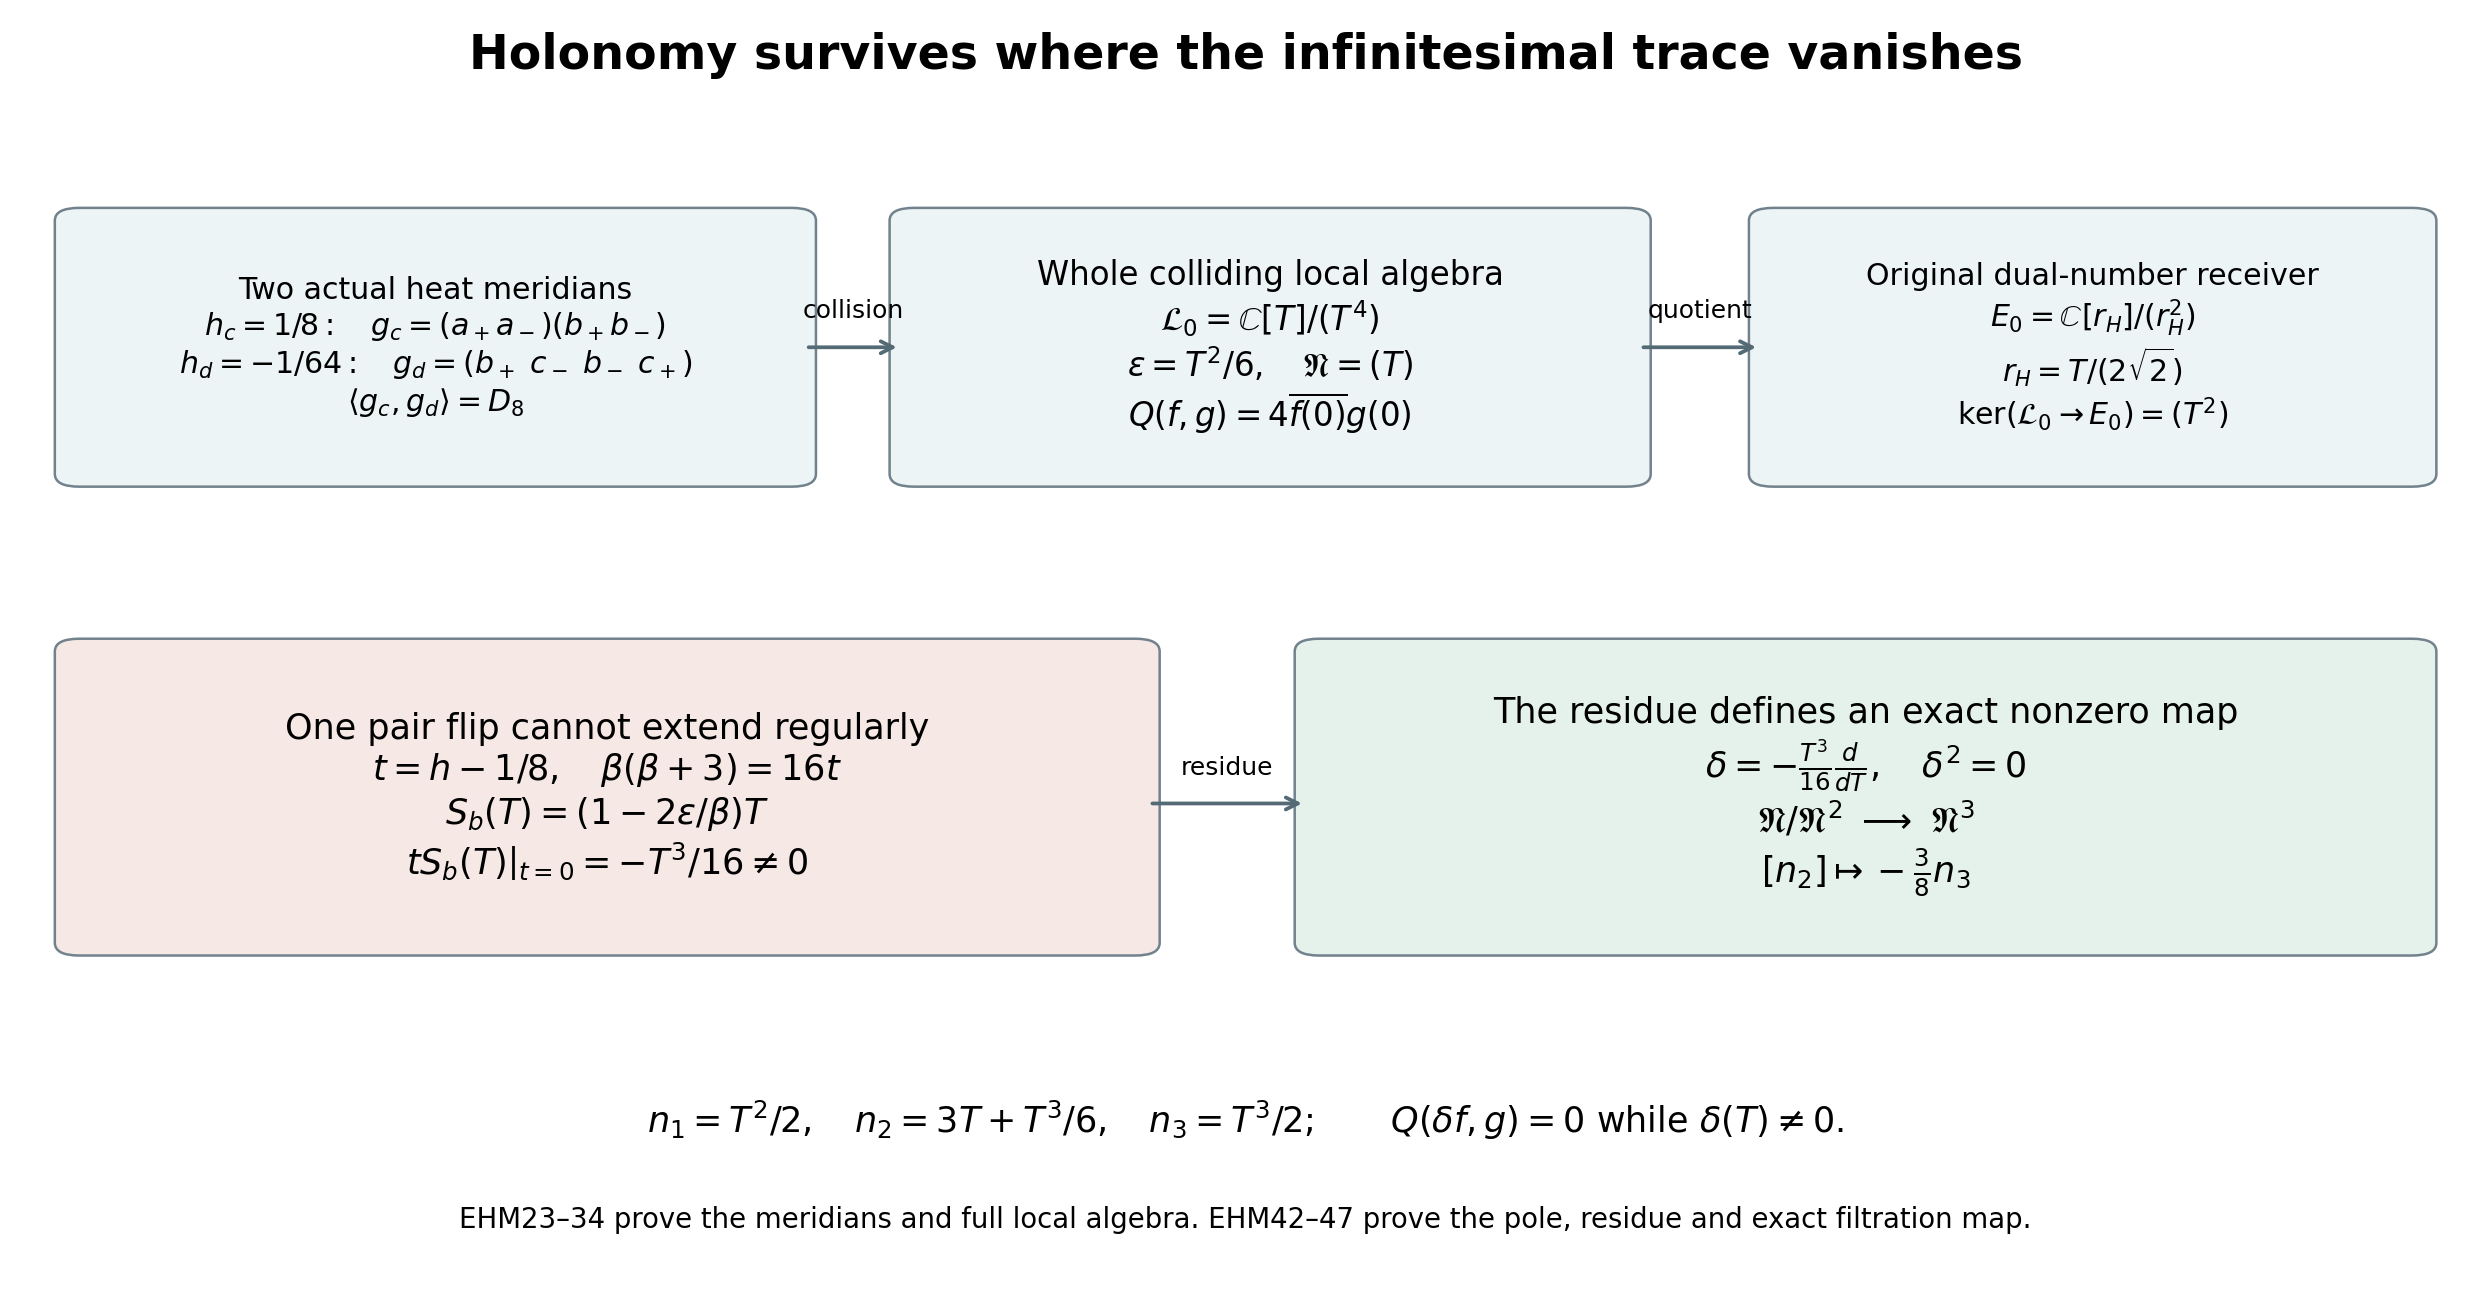
\includegraphics[keepaspectratio,alt={The two actual heat meridians, the full length-four collision algebra, its dual-number quotient, and the nonzero holonomy residue between infinitesimal layers. EHM23--EHM34 and EHM42--EHM47 give the complete proofs, signs and clock scale.}]{figures/33_holonomy_infinitesimal_residue.png}}
\caption{The two actual heat meridians, the full length-four collision
algebra, its dual-number quotient, and the nonzero holonomy residue
between infinitesimal layers. EHM23--EHM34 and EHM42--EHM47 give the
complete proofs, signs and clock scale.}
\end{figure}

\subsection{Exact residue-duality
continuation}\label{exact-residue-duality-continuation-2}

\href{COLLISION_RESIDUE_DUALITY_DERIVATION.md}{RD1--RD31b} proves the
complete Jacobian map from perfect residue duality to the retained
regular trace, identifies the actual packet radical with cotangent
cohomology, and computes the supported endpoint compensation. The
existing formulas and all their coordinates remain unchanged.

\clearpage

\section{Actual signed-cover averaging and the supported-zero
endpoint}\label{actual-signed-cover-averaging-and-the-supported-zero-endpoint}

This calculation uses the original eight-state completion and its actual
monodromy. It proves that averaging either of the two retained trace
forms over that group produces a positive semidefinite form, calculates
the complete defect, and evaluates the change on actual Weil tests. The
group action belongs to the auxiliary quartic cover. Its action on an
arithmetic global trace is not asserted.

The original cover and its full monodromy are proved in
\href{https://github.com/KokunoYumeto/zeta-function-research-reader/blob/ab45e221579a0d48ce2885b4ecdf1a6aefc24a20/workbenches/splitzero-tandem/continuations/20260920-fable-boundary-action/FABLE_TO_ORIGINAL_CONDUCTOR.tex\#L2097}{\emph{The
ES--Fable inverse correspondence in the original weighted conductor},
SM1--SM19, source lines2097--2513}. The exact fibre, trace and
involutions used here are proved in
\href{https://github.com/KokunoYumeto/zeta-function-research-reader/blob/d5c9d198a8432e3ede468b280162a99c00e3f4f7/workbenches/splitzero-tandem/branches/tau-zero-prime-positivity/EIGHT_STATE_HEAT_COMPARISON.md}{\emph{The
original eight-state heat comparison}, ESH9--ESH34}. The actual test
convention is
\href{https://github.com/KokunoYumeto/zeta-function-research-reader/blob/d5c9d198a8432e3ede468b280162a99c00e3f4f7/workbenches/splitzero-tandem/branches/tau-zero-prime-positivity/WEIL_ES_COMPENSATION_DERIVATION.md}{\emph{The
actual Weil correction has the ES three-plus-one form}, WEC1--WEC5}. The
Gaussian theta map below proves the endpoint comparison directly,
retaining supported zero.

\subsection{1. Exact fibre and point
coordinates}\label{exact-fibre-and-point-coordinates}

At the unchanged target \(\mathbf U_*=(0,0,-1,0)\), the completed
algebra is \[
\mathcal A=\mathbb C[R,T]/(R^3-R,T^2-3R^2+1)
\ \times\ \mathbb C[\Theta]/(\Theta^2+1).
\tag{HWA1}
\] Its eight geometric points, in the order retained throughout, are \[
X=(0+,0-,1+,1-,-1+,-1-,\infty+,\infty-)
\tag{HWA2}
\] with coordinates
\((0,\pm i),(1,\pm\sqrt2),(-1,\pm\sqrt2),(\infty,\pm i)\). Evaluation is
an algebra isomorphism \(\operatorname{ev}:\mathcal A\to\mathbb C^X\).
Indeed, the root indicators are
\(e_0=1-R^2,e_1=(R^2+R)/2,e_{-1}=(R^2-R)/2\). Inside a finite root
factor with chosen positive sign coordinate \(t_j\), its point
indicators are \(e_j(1\pm T/t_j)/2\). The infinity indicators are
\((1\mp i\Theta)/2\). These eight orthogonal idempotents sum to one,
evaluate as the eight coordinate vectors, and supply the inverse.
Multiplication is diagonal in this basis, so \[
\operatorname{Tr}_{\mathcal A}(x)=\sum_{p\in X}x_p.
\tag{HWA3}
\] No coordinate weighting is discarded: the coefficient basis and point
basis are related by the exact map \[
(c_j,d_j)\longmapsto(c_j+t_jd_j,c_j-t_jd_j),
\quad(t_0,t_1,t_{-1},t_\infty)=(i,\sqrt2,\sqrt2,i).
\tag{HWA4}
\]

Let \(\Sigma\) negate every sign coordinate and let \(\kappa\) conjugate
coefficients. The original native map is \(J(R,T)=(-R,-T)\),
\(J(v,\Theta)=(-v,\Theta)\), where \(v=1/R\) on the reciprocal chart.
Combining each with coefficient conjugation gives the following point
permutations: \[
q_\Sigma=(1+\ 1-)(-1+\ -1-),
\quad
q_J=(1+\ -1-)(1-\ -1+)(\infty+\ \infty-).
\tag{HWA5}
\] For example, conjugation at root0 swaps \(i,-i\), after which either
\(\Sigma\) or \(J\) swaps them back. At infinity \(J\) fixes \(\Theta\),
so conjugation still swaps the two points. Formula(HWA5) follows on all
eight points. If \(Q_q\) denotes the permutation matrix of the
involution \(q\), then \[
B_q(x,y)=\operatorname{Tr}(x^{\#_q}y)=x^*Q_qy.
\tag{HWA6}
\] Thus \(B_J\) has inertia \((5,3,0)\) and \(B_\Sigma\) has inertia
\((6,2,0)\): each swapped pair contributes eigenvalues \(1,-1\), and
each fixed point contributes1. The point metric here is the exact sum in
the regular trace, not the ES source metric.

\subsection{2. The actual order-192 group and its
average}\label{the-actual-order-192-group-and-its-average}

Label the four root pairs by \(j=0,1,-1,\infty\). The group proved in
SM1--SM19 is \[
G=\{(\sigma,\pi):\pi\in S_4,\ \sigma\in\{\pm1\}^4,
\ \prod_j\sigma_j=\operatorname{sgn}\pi\},
\quad(j,\epsilon)\mapsto(\pi(j),\sigma_j\epsilon).
\tag{HWA7}
\] There are exactly \(24\cdot8=192\) elements. For completeness, its
appearance in the actual quartic is determined by \(a_j^2H'(r_j)=1\) and
the invariant \(A^2\prod_{j<k}(r_k-r_j)\prod_ja_j\in\{1,-1\}\).
Exchanging adjacent roots along semicircles makes the moving derivatives
turn through \(\pi\), so their square roots yield four-cycles
\((j+\ (j+1)+\ j-\ (j+1)-)\). Their squares generate all even sign
patterns, and their root permutations generate \(S_4\); this proves
equality with(HWA7), as calculated with exact paths and coordinates in
SM7--SM12. The completed cover is unramified at the infinity pair
because its reciprocal equations have determinant
\(2\Theta k'(0)=2\Theta\ne0\). Paths from a nearby point with \(A\ne0\)
to \(\mathbf U_*\) transport its eight separate local charts.
Relabelling the roots and their chosen signs conjugates(HWA7) by a
signed permutation, which preserves the determinant-one subgroup. We
therefore use that same exact group on(HWA2).

Let \(P_g\) be its permutation matrix on point functions. Define the
explicitly scaled finite conjugation sum \[
\mathscr E(Q)=\frac1{192}\sum_{g\in G}P_g^*QP_g.
\tag{HWA8}
\] The factor \(1/192\) is part of the definition, so the unit vector
\(\mathbf1\), whose original trace square is8, still has square8. Let \[
P_{\rm ev}=\frac{I+P_\Sigma}{2},\qquad
P_{\rm c}=\frac{\mathbf1\mathbf1^*}{8}.
\tag{HWA9}
\] These are orthogonal projections for the point metric, respectively
onto sign-even functions and constant functions. Their kernels and ranks
follow directly: \(P_{\rm ev}\) replaces both values in each pair by
their arithmetic mean, so it has rank4; \(P_{\rm c}\) replaces every
value by the mean of all eight, so it has rank1.

The two exact averages are \[
\boxed{\mathscr E(Q_\Sigma)=P_{\rm ev},\qquad
\mathscr E(Q_J)=\frac13P_{\rm ev}+\frac23P_{\rm c}.}
\tag{HWA10}
\] Here is a direct proof without an assumed irreducibility theorem. The
even-sign kernel \(K\subset G\) has eight elements. On the sign-even
subspace it acts trivially. On the four-dimensional sign-odd subspace it
acts by the four distinct sign characters. For two distinct root indices
\(j,k\), the average of \(\sigma_j\sigma_k\) over \(K\) is zero: choose
a third root \(l\ne j,k\), and multiply each sign pattern by the one
flipping \(j,l\), which pairs opposite contributions. Hence averaging a
matrix on that subspace over \(K\) removes all off-diagonal entries.
Averaging then over the root permutations makes its diagonal constant,
equal to one quarter of its trace.

Both original matrices commute with \(\Sigma\), so there are no
even--odd blocks. For \(Q_\Sigma\), the even block is \(I_4\) and the
odd block is \(\operatorname{diag}(1,-1,-1,1)\), of trace0. Its odd
average therefore vanishes. For \(Q_J\), the odd block is \[
\begin{pmatrix}1&0&0&0\\0&0&-1&0\\0&-1&0&0\\0&0&0&-1\end{pmatrix},
\tag{HWA11}
\] also of trace0. Its even block is the transposition exchanging roots1
and−1. Averaging its conjugates over \(S_4\) averages the six
transpositions. The resulting matrix has diagonal \(3/6=1/2\) and every
off-diagonal entry \(1/6\), because a given index is fixed by three
transpositions and a specified distinct pair is exchanged by one. This
is \(I_4/3+\mathbf1_4\mathbf1_4^*/6\). Transport through the exact even
projection gives(HWA10).

For \(s_j(x)=x_{j+}+x_{j-}\), the complete quadratic formulas are \[
\begin{aligned}
\overline B_\Sigma(x,x)&=\frac12\sum_j|s_j(x)|^2,\\
\overline B_J(x,x)&=\frac16\sum_j|s_j(x)|^2
 +\frac1{12}\left|\sum_js_j(x)\right|^2.
\end{aligned}
\tag{HWA12}
\] Thus each has inertia \((4,0,4)\). For the native average its
eigenvalues on constants, the three-dimensional even sum-zero subspace,
and the four-dimensional odd subspace are respectively \(1,1/3,0\).
Their common radical is exactly \[
V_{\rm odd}=\{x:x_{j-}=-x_{j+}\ \text{for all four }j\}.
\tag{HWA13}
\] These formulas exhibit positivity from the actual finite group,
retaining every root and sign coordinate in the projection and its
kernel.

\subsection{3. Exact defect and multiplication retained by the odd
space}\label{exact-defect-and-multiplication-retained-by-the-odd-space}

Define, on the original eight-dimensional space, \[
D_q=Q_q-\mathscr E(Q_q).
\tag{HWA14}
\] For \(\Sigma\), the defect vanishes on even functions and is exactly
\(\operatorname{diag}(1,-1,-1,1)\) on odd functions. Its inertia is
\((2,2,4)\). For \(J\), the even block has eigenvalues
\(0,2/3,2/3,-4/3\), and the odd block is(HWA11), with eigenvalues
\(1,1,-1,-1\). To verify the even values, the root transposition fixes
the constant line and has eigenvalues \(1,1,-1\) on its sum-zero
complement; subtract its average \(1/3\) on that complement.
Consequently \[
\operatorname{inertia}(D_J)=(4,3,1).
\tag{HWA15}
\] The exact comparison for arbitrary vectors is \[
B_q(x,y)=\overline B_q(x,y)+x^*D_qy.
\tag{HWA16}
\] The average cannot be the regular trace paired with an antilinear
algebra involution on the original reduced \(\mathcal A\). Such an
involution permutes its eight primitive idempotents and conjugates their
coefficients; its trace matrix is an invertible permutation matrix
by(HWA3). The matrices in(HWA10) have rank4. This proves the stated
nonidentification and also identifies its exact four-dimensional
radical.

There is an explicit linear receiver and an exact multiplication defect.
Put \[
E:\mathbb C^X\to\mathbb C^4,
\quad E(x)_j=(x_{j+}+x_{j-})/2,
\quad O(x)_j=(x_{j+}-x_{j-})/2,
\tag{HWA17}
\] and let \(I:\mathbb C^4\to\mathbb C^X\) duplicate each root value.
Then \(EI=\operatorname{id}\), \(IE=P_{\rm ev}\),
\(\ker E=V_{\rm odd}\), and \[
E(xy)=E(x)E(y)+O(x)O(y).
\tag{HWA18}
\] All products on the right are coordinatewise. Expanding
\((a_j\pm b_j)(c_j\pm d_j)\) proves the identity in every coordinate.
Thus \(E\) is a retraction of vector spaces and a bimodule map over the
embedded sign-even algebra, while its displayed second term records
every product returning from odd to even support. In particular
\(z=e_{0+}-e_{0-}\) has \(E(z)=0\) but \(E(z^2)=e_0\ne0\). The kernel is
not an ideal, and(HWA17) is not silently promoted to an algebra
quotient.

The average forms factor exactly through \(E\): \[
\overline B_\Sigma(x,y)=2\sum_j\overline{E(x)_j}E(y)_j,
\quad
\overline B_J(x,y)=\frac23\sum_j\overline{E(x)_j}E(y)_j
 +\frac13\overline{\sum_jE(x)_j}\sum_jE(y)_j.
\tag{HWA19}
\] For any retained support lattice, applying these linear amplitude
maps to a supported module keeps its support coordinate unchanged. An
amplitude sent to0 therefore lands at the supported-zero element of that
same support, not at the unsupported element \(\tau\). Formula(HWA18)
remains the precise reason that this amplitude projection is not a
semiring homomorphism.

The average of vectors is a third, separately specified map: \[
\frac1{192}\sum_gP_gx=P_{\rm c}x,
\quad B_q(P_{\rm c}x,P_{\rm c}y)=x^*P_{\rm c}y.
\tag{HWA20}
\] The first identity follows because the group acts transitively on the
eight states, so each target coordinate receives each source coordinate
equally often. The second uses \(Q_q\mathbf1=\mathbf1\). This rank-one
form differs from both rank-four forms(HWA10); all three maps and their
different kernels are explicit.

\subsection{4. Actual supported-zero theta
endpoints}\label{actual-supported-zero-theta-endpoints}

Keep \(\mathcal T=C_c^\infty(\mathbb R;\mathbb C)\) and the programme
convention \[
M_f(s)=\int_{\mathbb R}f(v)e^{-(s-1/2)v}\,dv,
\qquad f^\#(v)=\overline{f(-v)}.
\tag{HWA21}
\] The transform of \(f^\#\) is \(\overline{M_f(1-\bar s)}\), by the
substitution \(v\mapsto-v\). Define the even Schwartz function \[
\phi_f(x)=\int_{\mathbb R}e^{v/2}f(v)e^{-\pi e^{2v}x^2}\,dv.
\tag{HWA22}
\] If \(\operatorname{supp}f\subset[-R,R]\), every derivative in \(x\)
of the integrand is a polynomial in \(x\) with bounded coefficients
times a Gaussian bounded by a constant times \(e^{-\pi e^{-2R}x^2}\).
Integration proves every Schwartz bound. The Fourier convention
\(\widehat\phi(y)=\int\phi(x)e^{-2\pi ixy}dx\) gives \[
\phi_f(0)=M_f(0),\quad \int\phi_f=M_f(1),
\quad\widehat{\phi_f}=\phi_{f(-\cdot)},
\quad\widehat{\overline{\phi_f}}=\phi_{f^\#}.
\tag{HWA23}
\] For the integral use \(\int e^{-\pi e^{2v}x^2}dx=e^{-v}\). For
Fourier use the same Gaussian scaling and substitute \(v\mapsto-v\).
Absolute integrability from the compact \(v\)-support justifies both
interchanges.

In \(G(\mathbb Z)=\{\tau\}\sqcup\mathbb Z\), let \(e\) denote
supported0. Its principal ideal \(\{\tau,e\}\) is prime: a product of
two nonzero supported integers is again nonzero supported, so a product
in that ideal has at least one factor there. The full supported theta is
\[
\Theta_f(x)=\sum_{n\in\mathbb Z}\phi_f(nx),\quad x>0,
\tag{HWA24}
\] and retains the \(n=0\) summand \(\phi_f(0)\) as the \(e\)-term. The
external \(\tau\) is a different label; no integer in this sum
represents it. Poisson summation for this Schwartz function gives
\(\Theta_f(x)=x^{-1}\Theta_{f(-\cdot)}(x^{-1})\). For this particular
mixture the identity follows directly by integrating the Gaussian theta
identity, with uniform absolute convergence for \(v\) in the compact
support. Its two endpoint amplitudes are exactly(HWA23), not an
arbitrary selected pair of complex numbers. Their regularized Mellin
endpoint terms are \[
-\frac{M_f(0)}s+\frac{M_f(1)}{s-1}.
\tag{HWA25}
\] Indeed split the integral of \(\Theta_f(x)-\phi_f(0)\) at1; use full
Poisson on \((0,1)\), and integrate \(x^{s-1}(x^{-1}M_f(1)-M_f(0))\).
Initially these elementary integrals converge for
\(\operatorname{Re}s>1\), and their displayed meromorphic expressions
supply continuation. The remaining transformed integrals over
\([1,\infty)\) are entire by rapid decay. Also direct Gaussian
integration in the initial half-plane gives \[
\int_0^\infty (\Theta_f(x)-\phi_f(0))x^{s-1}dx
=\pi^{-s/2}\Gamma(s/2)\zeta(s)M_f(s).
\tag{HWA26}
\] The two integer signs contribute2, cancelling the \(1/2\) in the
Gaussian Mellin integral. Uniform absolute convergence for
\(\operatorname{Re}s>1\) proves the exchange. This establishes both the
arithmetic amplitude and the exact endpoint residues from the retained
supported-zero theta.

For two actual tests the endpoint Hermitian pairing is \[
P_e(f,g)=\overline{M_f(0)}M_g(1)+\overline{M_f(1)}M_g(0).
\tag{HWA27}
\] This is the trace of the two-weight endpoint module with its Fourier
reflection exchanging the weights. It is the supported-zero endpoint
term; it is not all of the integrated Weil distribution. The separate
construction SZW retains the remaining finite-prime, archimedean and
fixed-support terms.

\subsection{5. Exact endpoint embedding and the change caused by
holonomy
averaging}\label{exact-endpoint-embedding-and-the-change-caused-by-holonomy-averaging}

Set \(A_f=M_f(0)\), \(B_f=M_f(1)\) and define \[
j:\mathcal T\to\mathbb C^X,
\quad j(f)=(0,0,A_f/\sqrt2,A_f/\sqrt2,
B_f/\sqrt2,B_f/\sqrt2,0,0).
\tag{HWA28}
\] The root assignment is stated in(HWA2): the two endpoint weights are
inserted into roots1 and−1. It is a linear comparison with scale
\(1/\sqrt2\), not a unital algebra map. By(HWA5),(HWA21), \[
j(f^\#)=\#_Jj(f),\qquad
B_J(j(f),j(g))=P_e(f,g).
\tag{HWA29}
\] Both formulas follow by exchanging \(A,B\) and conjugating; the two
signs at each root have equal values. Thus this is an exact
involution-preserving embedding of the two-dimensional endpoint quotient
into the actual completed trace.

The endpoint map \(f\mapsto(A_f,B_f)\) is onto. Here is a complete
section. Choose a positive smooth compact bump \(\psi\) on an open
interval. Put \(k_0(v)=e^{v/2}\), \(k_1(v)=e^{-v/2}\),
\(G_{ab}=\int\psi k_a\overline{k_b}\). For \(z\ne0\), the nonzero
combination \(\bar z_0e^{v/2}+\bar z_1e^{-v/2}\) cannot vanish on an
interval: multiplying by \(e^{v/2}\) would make \(\bar z_0e^v+\bar z_1\)
identically zero, whose derivative forces \(z_0=z_1=0\). Hence \(G\) is
positive definite. The function
\(S(A,B)=\psi\sum_b(G^{-1}(A,B)^T)_b\overline{k_b}\) has precisely those
two transforms by multiplication with \(G\). It is smooth and compactly
supported, proving surjectivity and \(\ker j=\{M_f(0)=M_f(1)=0\}\).

Substituting(HWA28) in(HWA12) gives the averaged endpoint form \[
\overline P_e(f,f)=\frac12(|A_f|^2+|B_f|^2)
 +\frac13\operatorname{Re}(\overline{A_f}B_f).
\tag{HWA30}
\] Its matrix is
\(\left(\begin{smallmatrix}1/2&1/6\\1/6&1/2\end{smallmatrix}\right)\),
with eigenvalues \(2/3,1/3\), so it is strictly positive on the endpoint
quotient. The exact change is \[
K_e=\overline P_e-P_e,
\quad
K_e(f,f)=\frac12(|A_f|^2+|B_f|^2)
-\frac53\operatorname{Re}(\overline{A_f}B_f).
\tag{HWA31}
\] In the explicitly related coordinates
\(u=(A+B)/\sqrt2,v=(A-B)/\sqrt2\), \[
P_e=|u|^2-|v|^2,
\quad\overline P_e=\frac23|u|^2+\frac13|v|^2,
\quad K_e=-\frac13|u|^2+\frac43|v|^2.
\tag{HWA32}
\] Thus actual tests with \((A,B)=(1,-1)\) have old value−2 and averaged
value \(2/3\), while tests with \((A,B)=(1,1)\) have old value2 and
averaged value \(4/3\). The section just proved supplies both tests. The
change has both signs on admissible tests, and its radical on
\(\mathcal T\) is exactly \(\ker j\): its two-dimensional matrix is
invertible and the section detects every nonzero endpoint vector.

The root-pair image of \(j\) is not invariant under the full group: a
signed root permutation taking root1 to root0 sends a vector with
\(A\ne0,B=0\) outside it. Such a permutation is in(HWA7) after choosing
signs with product equal to its permutation sign. This proves a specific
failure of invariance of this comparison map, with the group action and
endpoint map explicitly retained. It does not assert that every other
arithmetic comparison fails.

The full supported-zero construction
\href{https://github.com/KokunoYumeto/zeta-function-research-reader/blob/adfbfe74fa49e31cb7aa068cf755fb083be37c32/workbenches/splitzero-tandem/branches/tau-zero-prime-positivity/SUPPORTED_ZERO_PRIME_WEIL_DERIVATION.md}{\emph{The
supported-zero prime in the full theta and Weil trace distribution},
SZW24--SZW42} proves the actual integrated formula. Here are its
explicit terms and their exact transport. Put \(h=f^\#*g\), \(H=M_h\),
and retain \[
\begin{aligned}
\mathcal Z(f,g)&=\sum_\rho m_\rho\overline{M_f(1-\bar\rho)}M_g(\rho),\\
\mathcal A_\infty(f,g)&=\frac1{2\pi}\int_{\mathbb R}
\overline{\widehat f(t)}\widehat g(t)
\bigl(\operatorname{Re}\psi(1/4+it/2)-\log\pi\bigr)\,dt,\\
\mathcal P_{\rm fin}(f,g)&=\sum_{p,k\ge1}(\log p)p^{-k/2}
\{h(k\log p)+h(-k\log p)\}.
\end{aligned}
\tag{HWA33}
\] The sum in the last line is over primes \(p\) and integers \(k\ge1\).
It is finite for each compactly supported \(h\). The absolutely
convergent zero sum and archimedean integral, with their complete proof
and the original minus-exponent convention, are SZW24--SZW32.
Substituting \(P_e=\overline P_e-K_e\) gives the actual equality \[
\boxed{\mathcal Z=P_e+\mathcal A_\infty-\mathcal P_{\rm fin}
=\overline P_e+\mathcal A_\infty-\mathcal P_{\rm fin}-K_e.}
\tag{HWA34}
\] Formula(HWA31) gives the entire changed term on every admissible
test. In particular the negative endpoint \(-2\) becomes \(2/3\), while
its retained complement changes by \(-8/3\). This is an exact
calculation inside the derived supported-zero formula.

The full labels can be kept before any scalar projection. Let \(L\) be
the finite fixed-support lattice of SZW10--SZW13, \(\mathbf e_1\) its
top coordinate, and
\(\mathbf s_< =\sum_{\lambda\ne1}\mathbf e_\lambda\). Here lower labels
are distinct fixed zero points, not the independently different
coordinatewise adelic support construction. The original labelled
formula, now on \(h=f^\#*g\), is \[
\begin{aligned}
\boldsymbol B&=P_e\mathbf e_1+H(0)\mathbf s_<,\\
\boldsymbol D&=(\mathcal P_{\rm fin}-\mathcal A_\infty)\mathbf e_1+H(0)\mathbf s_<,\\
\boldsymbol B-\mathcal Z\mathbf e_1&=\boldsymbol D.
\end{aligned}
\tag{HWA35}
\] Keeping these lower fixed distributions exactly and applying the
holonomy comparison at the top endpoint gives \[
\begin{aligned}
\overline{\boldsymbol B}&=\overline P_e\mathbf e_1+H(0)\mathbf s_<,\\
\overline{\boldsymbol D}&=(\mathcal P_{\rm fin}-\mathcal A_\infty+K_e)\mathbf e_1
 +H(0)\mathbf s_<,\\
\overline{\boldsymbol B}-\mathcal Z\mathbf e_1&=\overline{\boldsymbol D}.
\end{aligned}
\tag{HWA36}
\] This follows by adding precisely \(K_e\mathbf e_1\) to both sides
of(HWA35). No lower support trace was merged with the top endpoint or
discarded.

For the minimal Fourier-closed endpoint module proved in SZW40--SZW42,
every lower fixed constant acquires its exact weight-one Dirac partner.
Its labelled boundary and geometric distributions are \[
\boldsymbol B^{\mathcal F}=P_e(\mathbf e_1+\mathbf s_<),\quad
\boldsymbol D^{\mathcal F}=(\mathcal P_{\rm fin}-\mathcal A_\infty)\mathbf e_1+P_e\mathbf s_<.
\tag{HWA37}
\] There is now the defined direct-sum comparison
\(\bigoplus_{\lambda\in L}j\) from the independent endpoint tests into
one completed eight-state vector space for each label. Averaging its
native forms label by label and restricting back to the diagonal actual
scalar tests gives \[
\begin{aligned}
\overline{\boldsymbol B}^{\mathcal F}&=\overline P_e(\mathbf e_1+\mathbf s_<),\\
\overline{\boldsymbol D}^{\mathcal F}&=
(\mathcal P_{\rm fin}-\mathcal A_\infty+K_e)\mathbf e_1
 +\overline P_e\mathbf s_<,\\
\overline{\boldsymbol B}^{\mathcal F}-\mathcal Z\mathbf e_1
&=\overline{\boldsymbol D}^{\mathcal F}.
\end{aligned}
\tag{HWA38}
\] Proof: add \(K_e\) on every label in(HWA37), using the original
identity
\(\boldsymbol B^{\mathcal F}-\mathcal Z\mathbf e_1=\boldsymbol D^{\mathcal F}\).
The direct-sum comparison is a specified linear map, and(HWA29) proves
its involution compatibility on each summand. The group is the actual
auxiliary-cover group on each receiver; no unproved action on the
arithmetic zeros or on the original test space has been introduced. Thus
the positive averaged boundary, its full geometric correction, the
supported-zero prime, the unsupported coordinate and every mixed-support
label are retained in one exact identity.

\begin{figure}
\centering
\pandocbounded{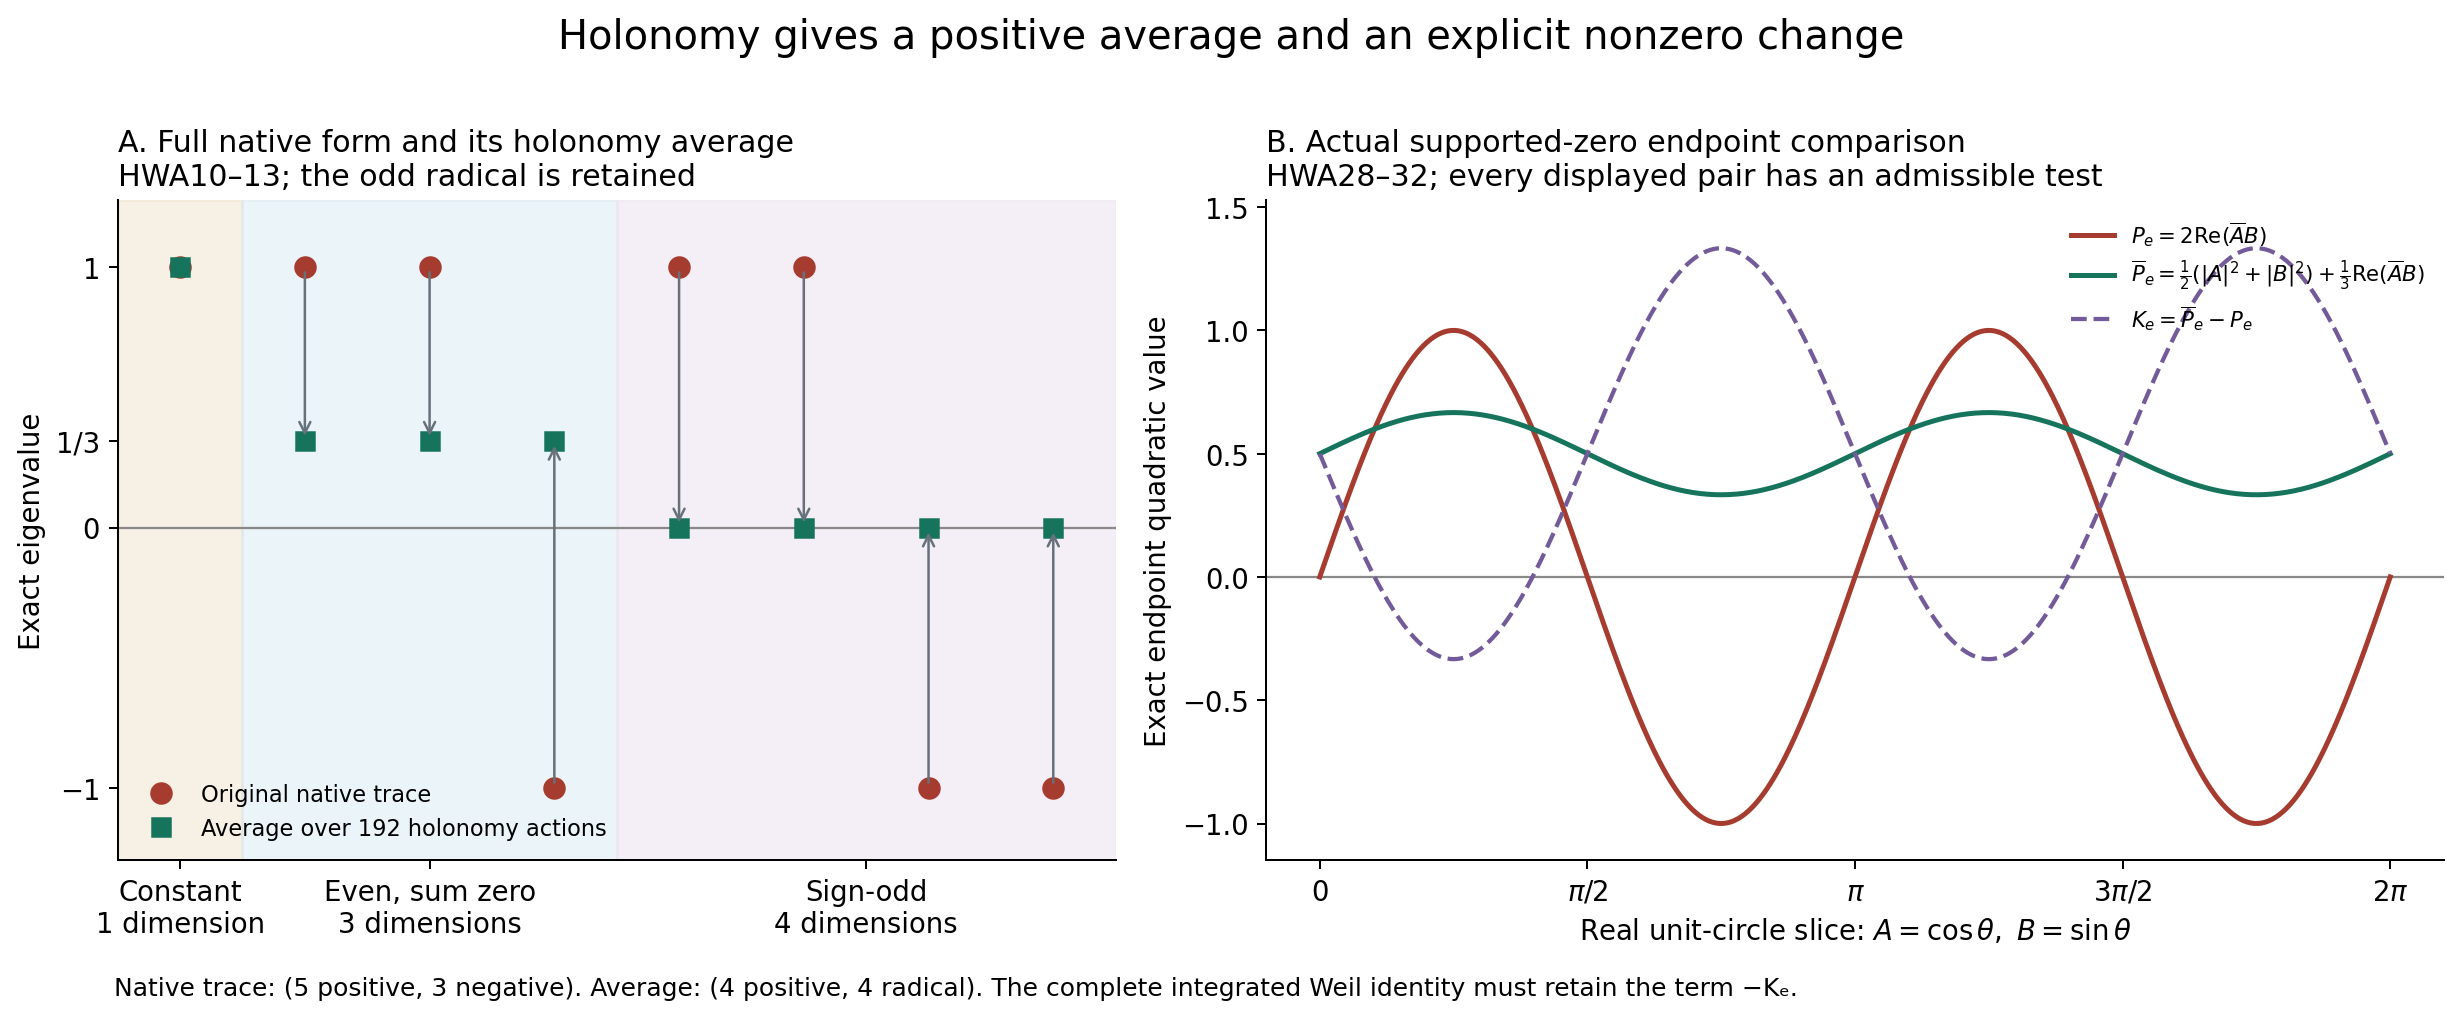
\includegraphics[keepaspectratio,alt={The complete native trace spectrum before and after its order-192 holonomy average, and the exact supported-zero endpoint comparison on actual admissible tests. HWA10--HWA15 prove the left panel; HWA28--HWA32 prove the right panel; HWA34--HWA38 retain its change in the full supported-zero formula.}]{figures/31_holonomy_endpoint_average.png}}
\caption{The complete native trace spectrum before and after its
order-192 holonomy average, and the exact supported-zero endpoint
comparison on actual admissible tests. HWA10--HWA15 prove the left
panel; HWA28--HWA32 prove the right panel; HWA34--HWA38 retain its
change in the full supported-zero formula.}
\end{figure}

\subsection{Exact full-form
continuation}\label{exact-full-form-continuation-1}

The \href{CAUCHY_REFLECTION_INDEX_DERIVATION.md}{reflection-index
theorem, NI1--32}, calculates the signed index of every complete Cauchy
coefficient tail. The
\href{FINITE_JET_COMPLEMENT_AND_HEAT_TRUNCATION.md}{finite-jet and
endpoint proof, FJ1--29}, preserves the exact finite jets while proving
density on the remaining zeros, derives the full exterior index and
tail, and calculates the second and third actual heat coefficients. All
supported endpoints remain explicit. These results identify the
remaining sign problem without asserting its resolution.

\clearpage

\section{Prime holonomy in the supported-zero Weil
distribution}\label{prime-holonomy-in-the-supported-zero-weil-distribution}

The prime-orbit holonomy here is the actual arithmetic Frobenius in the
finite abelian covers constructed by Alain Connes and Caterina Consani,
\emph{Knots, primes and class field theory},
\href{https://arxiv.org/abs/2501.06560v1}{arXiv:2501.06560v1}. The
original author source was read at lines 464--695: Definition
\texttt{coverdef}, Lemma \texttt{Gacts}, Proposition
\texttt{mappingtorus}, Theorem \texttt{mappingtorus1}, Fact
\texttt{artinrec}, Theorem \texttt{main}, and Remark
\texttt{archimedeanplace}. Root subsequently read the entire body and
bibliography. Their finite cover and its arithmetic identification are
prior results. The formulas below derive its oriented trace, inertia
maps, fixed-support endpoints, character-resolved Euler factors, and
exact comparison with SZW. They do not identify an unrelated
finite-group action with this arithmetic cover.

The full supported-zero object, its prime spectrum, test convention, and
trace receiver are those proved in
\href{https://github.com/KokunoYumeto/zeta-function-research-reader/blob/adfbfe74fa49e31cb7aa068cf755fb083be37c32/workbenches/splitzero-tandem/branches/tau-zero-prime-positivity/SUPPORTED_ZERO_PRIME_WEIL_DERIVATION.md}{the
full supported-zero Weil proof}, SZW1--SZW47. In particular \[
S=G(\mathbb Z)=\{\tau\}\sqcup\mathbb Z^\bullet,
\qquad e=0^\bullet\ne\tau,
\qquad(\tau)\subsetneq(e)\subsetneq(p).
\tag{PHW1}
\] Both zero points will remain separate. No expression \(\log0\),
positive period for a fixed point, or numerical Euler factor for \(e\)
is introduced.

\subsection{1. The finite cover, inertia, and the two orientation
coordinates}\label{the-finite-cover-inertia-and-the-two-orientation-coordinates}

Put \(K=\widehat{\mathbb Z}^{\times}\), and let
\(\chi:K\twoheadrightarrow G\) be a continuous surjection to a finite
abelian group. Use exactly the source's balanced quotient \[
X^\chi=(Y_{\mathbb Q}\times G)/K,
\qquad (z,g)\sim(zw,\chi(w)g),
\qquad Y_{\mathbb Q}=\mathbb Q^\times\backslash\mathbb A_{\mathbb Q}.
\tag{PHW2}
\] The group \(G\) acts on the right in the second coordinate. At a
prime \(p\), define \[
I_p=\chi(\mathbb Z_p^\times),\qquad
\widetilde p_p=1,\quad \widetilde p_\ell=p\ (\ell\ne p),
\qquad g_p=\chi(\widetilde p)\in G,
\qquad \ell_p=\log p>0.
\tag{PHW3}
\] Here \(\widetilde p\in K\); at every \(\ell\ne p\), the rational
integer \(p\) is an \(\ell\)-adic unit. The class of \(g_p\) in
\(G/I_p\) is independent of a change of the \(p\)-component. At an
unramified prime \(I_p=1\), this is the source's
\(\chi(p)=\mathrm{Frob}_p\), the arithmetic Frobenius. At ramified
primes the same quotient class acts on the inertia-invariant fibre.

For completeness the actual orientation map follows directly from
(PHW2). Before the finite quotient, the source identifies the inverse
image of \(C_p\) with
\(p^{\mathbb Z}\backslash(H_p\times\mathbb R_+^\times)\), where
\(H_p=\prod_{\ell\ne p}\mathbb Z_\ell^\times\) and the generator is
\((h,\lambda)\mapsto(ph,p\lambda)\). Write \(t=\log\lambda\). Reducing
\((h,g)\) by the compact action gives the natural fibre coordinate
\(g_0=\chi(h)^{-1}g\), modulo \(I_p\). Thus the finite mapping torus is
exactly \[
\mathfrak C_p=
\bigl((G/I_p)\times\mathbb R\bigr)
\big/\bigl((g,t)\sim(g_p^{-1}g,t+\ell_p)\bigr).
\tag{PHW4}
\] The equality \(\chi(ph)^{-1}g=g_p^{-1}\chi(h)^{-1}g\) proves the
formula. This proof also gives the ramified version, since the missing
\(p\)-unit coordinate acts on the fibre by \(I_p\). The positive flow is
\([g,t]\mapsto[g,t+a]\). Its first return from \(t=0\) to \(t=\ell_p\),
expressed again at \(t=0\), is \(g\mapsto g_pg\). The opposite traversal
is \(g\mapsto g_p^{-1}g\).

The map \((g,t)\mapsto(g^{-1},t)\) turns (PHW4) into the displayed
source convention with generator \((g,t)\mapsto(g_pg,t+\ell_p)\). It
intertwines right deck multiplication by \(k\) with multiplication by
\(k^{-1}\). This is the exact coordinate conversion; using the printed
generator without this conversion would reverse the fibre
representation. The arithmetic Frobenius and its inverse are both
retained below.

Let \(V\) be a finite-dimensional complex unitary representation
\(\rho\) of \(G\). Define \[
P_{I_p}=\frac1{|I_p|}\sum_{i\in I_p}\rho(i),
\qquad V_p=V^{I_p}=\operatorname{im}P_{I_p},
\qquad T_p=\rho(g_p)|_{V_p}.
\tag{PHW5}
\] Direct multiplication of the finite sums shows \(P_{I_p}^2=P_{I_p}\);
unitarity gives \(P_{I_p}^*=P_{I_p}\). It fixes precisely the invariant
vectors. Since \(G\) is abelian, \(T_p\) is a well-defined unitary
operator on \(V_p\), unchanged by replacing \(g_p\) by \(g_pi\),
\(i\in I_p\). No assumption about unramified primes is needed in this
formula.

\subsection{2. An actual trace on every prime
circle}\label{an-actual-trace-on-every-prime-circle}

The coefficient space of sections over (PHW4) is \[
\mathcal H_{p,V}=
\{v\in L^2_{\mathrm{loc}}(\mathbb R,V_p):
v(t+\ell_p)=T_p^{-1}v(t)\},
\qquad
\|v\|^2=\int_0^{\ell_p}\|v(t)\|^2dt.
\tag{PHW6}
\] Indeed a function on the natural fibre satisfying
\(F(gk,t)=\rho(k)^{-1}F(g,t)\) has precisely this boundary condition
after (PHW4). The unitary flow on sections is inverse pullback,
\(U_p(a)v(t)=v(t-a)\); consequently \(U_p(\ell_p)=T_p\). For
\(\nu\in C_c^\infty(\mathbb R)\), the bounded operator \[
A_{p,V}(\nu)=\int_{\mathbb R}\nu(a)U_p(a)\,da
\tag{PHW7}
\] is trace class, and its full trace, including the zero iterate, is \[
\boxed{
\operatorname{Tr}A_{p,V}(\nu)
=\ell_p\sum_{k\in\mathbb Z}\operatorname{Tr}(T_p^k)\nu(k\ell_p).
}
\tag{PHW8}
\] Here and below \(\operatorname{Tr}(T_p^k)\) means the trace of the
matrix power; it is not the power of its trace. To prove (PHW8),
diagonalize \(T_p\). For an eigenvalue \(e^{i\theta}\), an orthonormal
Fourier basis is \(\ell_p^{-1/2}e^{i(2\pi n-\theta)t/\ell_p}\),
\(n\in\mathbb Z\). The eigenvalues of (PHW7) are
\(\widehat\nu((2\pi n-\theta)/\ell_p)\), with the minus Fourier
convention. They are absolutely summable by repeated integration by
parts. Poisson summation of this Schwartz function gives \[
\sum_{n\in\mathbb Z}\widehat\nu((2\pi n-\theta)/\ell_p)
=\ell_p\sum_{k\in\mathbb Z}e^{ik\theta}\nu(k\ell_p).
\tag{PHW9}
\] For example this equality follows by expanding the periodic Dirac
distribution
\(\sum_n e^{-2\pi i n a/\ell_p}=\ell_p\sum_k\delta(a-k\ell_p)\), whose
Fourier coefficients on one period are all one, and multiplying by
\(\nu(a)e^{i\theta a/\ell_p}\). Summing the finitely many eigenlines
proves (PHW8), including the term \(\ell_p\dim(V_p)\nu(0)\).

The original supported Weil test space remains \[
\mathcal T=C_c^\infty(\mathbb R;\mathbb C),\qquad
H(s)=M_h(s)=\int h(v)e^{-(s-1/2)v}dv,
\qquad f^\#(v)=\overline{f(-v)}.
\tag{PHW10}
\] Choose once and for all an even smooth cutoff \(\kappa\), zero for
\(|a|\le\tfrac14\log2\) and one for \(|a|\ge\tfrac12\log2\). Such a
function is obtained from \(b(x)=e^{-1/x}\) for \(x>0\), zero otherwise,
using \(b(x)/(b(x)+b(1-x))\) on the intervening interval; its even
extension is smooth because it is constant near zero. Define the exact
map \[
\nu_h(a)=\kappa(a)e^{-|a|/2}h(-a)\in C_c^\infty(\mathbb R).
\tag{PHW11}
\] The cutoff is identically one at every nonzero prime iterate
\(\pm k\log p\), so (PHW8) gives \[
\boxed{
P_V(h)=\sum_p\operatorname{Tr}A_{p,V}(\nu_h)
=\sum_p\sum_{k\ge1}(\log p)p^{-k/2}
\left\{\operatorname{Tr}(T_p^k)h(-k\log p)
+\operatorname{Tr}(T_p^{-k})h(k\log p)\right\}.
}
\tag{PHW12}
\] The trace sum in this formula has only finitely many nonzero terms:
if \(\operatorname{supp}h\subset[-R,R]\), then \(k\log p\le R\). It is
independent of every permitted choice of \(\kappa\). This proves the
actual comparison between the original prime-orbit circle and the
weighted Weil distribution. The weight \(e^{-|a|/2}\) is an explicit
test map; its arithmetic contour identity is proved in (PHW23) below.
The omitted identity iterate is exactly the separately known functional
\(\ell_p\dim(V_p)\nu(0)\) of (PHW8).

There is a necessary operator-domain distinction even though (PHW12) is
a complete distribution. The bounded direct sum
\(\bigoplus_p A_{p,V}(\nu)\) exists, with norm at most \(\|\nu\|_1\),
but for nonzero \(V\) and nonzero \(\nu\) it is not trace class. To
prove this, \(\widehat\nu\) is not identically zero by Fourier
inversion, so there is a real interval of positive length on which
\(|\widehat\nu|\ge c>0\). All but finitely many \(p\) have
\(V_p=V\ne0\). In any eigenline the frequency grid has spacing
\(2\pi/\ell_p\), so the number of grid points in that interval is at
least its length times \(\ell_p/(2\pi)-1\). The trace norm of the
corresponding diagonal block therefore grows at least as a positive
constant times \(\log p\). The total trace norm diverges. For
\(\nu=\nu_h\), the finite-prime-cutoff traces nevertheless stabilize
once \(p>e^R\), by (PHW8). Thus (PHW12) is an exact stabilized trace
distribution, not an ordinary trace on the infinite direct sum. The
operator family, the finite cutoffs, the stabilized trace, and the
failure of the full trace-class norm are all retained.

\subsection{3. Determinants and the character-resolved arithmetic
map}\label{determinants-and-the-character-resolved-arithmetic-map}

For \(\Re s>1\), define \[
L_V(s)=\prod_p\det(1-p^{-s}T_p\mid V_p)^{-1}.
\tag{PHW13}
\] Since every eigenvalue of \(T_p\) has modulus one and
\(\dim V_p\le\dim V\), the logarithm \[
\log L_V(s)=\sum_p\sum_{k\ge1}\frac{\operatorname{Tr}(T_p^k)}k p^{-ks},
\qquad
-\frac{L_V'}{L_V}(s)=
\sum_p\sum_{k\ge1}(\log p)\operatorname{Tr}(T_p^k)p^{-ks}
\tag{PHW14}
\] converges absolutely, uniformly on every half-plane
\(\Re s\ge1+\varepsilon\), with its differentiated series. Indeed it is
dominated respectively by constant multiples of
\(\sum_{n\ge2}n^{-1-\varepsilon}\) and
\(\sum_{n\ge2}(\log n)n^{-1-\varepsilon}\). The determinant identity
follows by applying \(-\log(1-z)=\sum_{k\ge1}z^k/k\) to each eigenvalue.
In particular these formulas specify the branch of the logarithm and
prove that \(L_V\) has no zero or pole in this half-plane.

Let \(\widehat G\) denote the character group. The explicit mutually
orthogonal idempotents are \[
P_\eta=\frac1{|G|}\sum_{g\in G}\overline{\eta(g)}\rho(g),
\qquad V=\bigoplus_{\eta\in\widehat G}V_\eta,
\quad V_\eta=\operatorname{im}P_\eta,
\quad m_\eta=\dim V_\eta.
\tag{PHW15}
\] For a nontrivial character \(\alpha\), the sum \(\sum_g\alpha(g)\) is
zero: multiplication of its index by an element where \(\alpha\ne1\)
multiplies the sum by that unequal value. This proves the orthogonality
identities for (PHW15). Simultaneous diagonalization of the commuting
unitary matrices proves completeness; every eigenline supplies one of
the characters, and (PHW15) projects onto it.

The character \(\eta\circ\chi\) factors through a finite unit group. At
every prime choose its smallest local congruence exponent through which
it factors, and take the product of those prime powers. This gives its
conductor \(q_\eta\) and a primitive Dirichlet character \(\eta_0\)
modulo \(q_\eta\). Set \(a_\eta\in\{0,1\}\) by
\(\eta(\chi(-1))=(-1)^{a_\eta}\). At \(p\), the summand \(V_\eta\) lies
in \(V_p\) precisely when \(p\nmid q_\eta\); its eigenvalue is then
\(\eta_0(p)\). This follows by restricting \(\eta\circ\chi\) to the
\(p\)-unit group and evaluating \(\widetilde p\) at the remaining
conductor components. Therefore (PHW13) is exactly \[
L_V(s)=\prod_{\eta\in\widehat G}L(s,\eta_0)^{m_\eta}.
\tag{PHW16}
\] This includes primes ramified in the extension but unramified for a
particular character: they have not been removed merely because they
divide the conductor of the whole cover. The trivial character has
\(q_1=1\), \(a_1=0\), and \(L(s,1)=\zeta(s)\).

There is a fully labelled version before taking a representation trace.
In \(\mathbb C[G]\), put \(E_I=|I|^{-1}\sum_{i\in I}i\). Define \[
\mathscr P_G(h)=\sum_{p,k\ge1}(\log p)p^{-k/2}
\left\{E_{I_p}g_p^k h(-k\log p)
+E_{I_p}g_p^{-k} h(k\log p)\right\}.
\tag{PHW17}
\] It is a finite sum for every test. Applying \(\operatorname{Tr}\rho\)
gives (PHW12), because \(\rho(E_I)=P_I\). The character Fourier map
\(x\mapsto(\eta(x))_\eta\) is an isomorphism
\(\mathbb C[G]\to\mathbb C^{\widehat G}\), with inverse given by the
character idempotents; its orthogonality proof is the same finite-sum
calculation as (PHW15). Hence no holonomy character is lost before a
projection is specified.

The trivial-character observation is augmentation
\(\epsilon(\sum c_g g)=\sum c_g\). Its kernel is the span of the
elements \(g-1\), and its exact section is \(c\mapsto cE_G\). Indeed
\(\epsilon(E_G)=1\), \(gE_G=E_G\), and every coefficient vector of total
zero equals \(\sum c_g(g-1)\). Consequently \[
\epsilon\mathscr P_G=P_{\mathrm{fin}},
\qquad E_G\mathscr P_G=P_{\mathrm{fin}}E_G,
\qquad
\mathscr P_G=P_{\mathrm{fin}}E_G+(1-E_G)\mathscr P_G.
\tag{PHW18}
\] The second term contains exactly the nontrivial character components;
it is an explicitly retained augmentation-ideal distribution. The first
is the original arithmetic prime term of SZW24, with its original
\(\log p\) and \(p^{-k/2}\) constants.

\subsection{4. The fixed-support endpoints of the same
cover}\label{the-fixed-support-endpoints-of-the-same-cover}

At the global supported zero \(e\in G(\mathbb A_{\mathbb Q})\), every
element of \(K\) fixes the point. Thus its fibre in (PHW2) is
\(G/\chi(K)=G/G\), a singleton. Extending the same construction to the
full fixed-sector carrier \(G_L(\mathbb A_{\mathbb Q})\) gives a
separate singleton above each \(z_\lambda\), including \(e_L\) and
\(\tau_L\). The balanced quotient never relates two distinct support
labels. Coefficients in \(V\) over each such fibre are therefore \[
W=V^G=\operatorname{im}P_G,
\qquad P_G=\frac1{|G|}\sum_{g\in G}\rho(g),
\qquad V=W\oplus\ker P_G.
\tag{PHW19}
\] These maps are actual stabilizer invariants, not a hypothesis of
holonomy-invariant test functions. The same averaging proof as (PHW5)
shows that \(P_G\) is a projection, and (PHW15) identifies its kernel as
the sum of all nontrivial character spaces. Let \(m_0=\dim W=m_1\).

The exact Schwartz domain verifies both endpoint weights. Use \[
\mathcal F_{L,V}=
\{f\in\mathcal S(\mathbb A_{\mathbb Q})\otimes V:
f(aw)=\rho(\chi(w))^{-1}f(a)\ (w\in K)\}
\oplus\bigoplus_{\lambda\ne1_L}W_\lambda.
\tag{PHW20}
\] Evaluation gives \(f(0)\in W\), since zero is fixed by every \(w\).
The integral \(\int f\) also lies in \(W\), because multiplication by a
compact unit preserves the specified self-dual additive Haar measure.
Thus \[
\beta_{L,V}(f,c)=\left(f(0),\int f,(c_\lambda)\right),
\qquad
B_{L,V}=W(0)_e\oplus W(1)_{e^\vee}
\oplus\bigoplus_{\lambda\ne1_L}W(0)_\lambda.
\tag{PHW21}
\] The map is onto: for \(w\in W\), embed an even real Schwartz test as
\(\phi\otimes1_{\widehat{\mathbb Z}}\otimes w\), use the two moment
preimages proved in SZW13, and prescribe the lower coefficients
independently. Its kernel is exactly \(f(0)=\int f=0\) and all
\(c_\lambda=0\). Dilation by an idele fixes the first and lower
coordinates and multiplies the integral by its norm, proving the stated
weights. This connects the same coefficient system's prime-orbit spaces
(PHW6) to its fixed-support quotient without identifying their carriers.

On the original SZW test \(q_h(j)=|j|^{-1/2}h(-\log|j|)\), the
label-resolved boundary trace is consequently \[
\boldsymbol B_{L,V}(h)
=m_0\left((H(0)+H(1))\mathbf e_{1_L}
+H(0)\sum_{\lambda\ne1_L}\mathbf e_\lambda\right).
\tag{PHW22}
\] The coefficient is \(\dim V^G\), not \(\dim V\). The original
two-point case has its separate \(\tau\)-term \(m_0H(0)\), while the
supported-zero/Fourier pair contributes \(m_0(H(0)+H(1))\). The Fourier
closure of SZW40--42 tensors with \(W\), so it adds exactly
\((|L|-1)m_0\) weight-one partners and no partners in the nontrivial
character spaces.

For a finite prime orbit the zero-coordinate set is instead \(\{p\}\),
giving inertia \(I_p\) and the circle (PHW4). Its adelic zero-coordinate
prime contracts to \((e)\subset S\), by SZW4, but its other nonzero
coordinates and its place label remain present. Thus contraction to the
supported-zero prime does not collapse these circles into the global
zero point. The source's archimedean orbit has fibre
\(G/\langle\chi(-1)\rangle\); its invariant coefficient space is the
even-parity sum in (PHW15). This is another actual stabilizer map,
distinct from both global \(G\)-invariants and finite-prime inertia
invariants.

\subsection{5. The convergent arithmetic contour and the full trivial
sector}\label{the-convergent-arithmetic-contour-and-the-full-trivial-sector}

Let \(V^\vee\) be the dual representation, so the local traces are those
of \(T_p^{-k}\). For every \(c>1\), the Euler series already proved in
(PHW14) gives \[
\begin{aligned}
P_V(h)={}&\frac1{2\pi i}\int_{c-i\infty}^{c+i\infty}
-\frac{L_V'}{L_V}(s)H(s)\,ds\\
&+\frac1{2\pi i}\int_{c-i\infty}^{c+i\infty}
-\frac{L_{V^\vee}'}{L_{V^\vee}}(s)H(1-s)\,ds.
\end{aligned}
\tag{PHW23}
\] These are absolutely convergent integrals: the logarithmic derivative
is bounded on each indicated vertical line by its absolutely convergent
Euler series, and the transforms decrease faster than every power of the
height by integration by parts. Termwise integration is therefore valid.
To compute the first integral term with \(\ell=k\log p\), Fourier
inversion gives \[
\frac1{2\pi}\int_{\mathbb R}e^{-it\ell}H(c+it)\,dt
=h(-\ell)e^{(c-1/2)\ell}.
\] Multiplication by \(p^{-kc}=e^{-c\ell}\) gives \(p^{-k/2}h(-\ell)\).
Replacing \(H(s)\) by \(H(1-s)\) gives \(p^{-k/2}h(\ell)\); the dual
representation supplies \(\operatorname{Tr}(T_p^{-k})\). This proves
(PHW23) with the original signs and weights. This argument uses only the
convergent half-plane, not a presumed functional equation for an
arbitrary representation.

For the trivial character, both integrals and the fixed-support
endpoints are exactly those in SZW. Writing \(E_G=|G|^{-1}\sum_g g\) in
the group algebra, the exact retained decomposition is \[
\mathscr P_G=P_{\mathrm{fin}}E_G+\mathscr P_G^{\mathrm{aug}},\qquad
\mathscr P_G^{\mathrm{aug}}=(1-E_G)\mathscr P_G,\qquad
\epsilon\mathscr P_G^{\mathrm{aug}}=0.
\tag{PHW24}
\] Its proof is (PHW18); its kernel is the full augmentation ideal, not
a declaration that the complementary distribution vanishes. The trace
receiving \(P_{\mathrm{fin}}\) is the complete supported-zero identity
\[
\begin{aligned}
\boldsymbol B_L&=(H(0)+H(1))\mathbf e_{1_L}
+H(0)\sum_{\lambda\ne1_L}\mathbf e_\lambda,\\
\boldsymbol Z_L&=Z(h)\mathbf e_{1_L},\\
\boldsymbol D_L&=(P_{\mathrm{fin}}-A_\infty)\mathbf e_{1_L}
+H(0)\sum_{\lambda\ne1_L}\mathbf e_\lambda,\\
\boldsymbol B_L-\boldsymbol Z_L&=\boldsymbol D_L.
\end{aligned}
\tag{PHW25}
\] The proof is SZW20--SZW34: the full theta lift gives the endpoints,
the convergent contour gives the arithmetic identity, and its explicit
divisor receiver gives \(Z(h)\). Tensoring with the invariant
coefficient space \(W\) multiplies every term by \(\dim W\), by the
trace of an identity tensor factor. The Fourier closure tensors likewise
with \(W\), retaining every support label and its partner. This is the
actual trivial-sector map from the holonomy construction into the
programme formula. Equations (PHW17), (PHW23), and (PHW24) retain the
other character-resolved arithmetic distributions with their full Euler
data. The explicit signed-cover quotient which reaches a nontrivial one
of these sectors is proved in
\href{https://github.com/KokunoYumeto/zeta-function-research-reader/blob/4a4238afc992e77aee83b97d38a1a63d283f540c/workbenches/splitzero-tandem/branches/tau-zero-prime-positivity/CLASS_FIELD_SIGNED_HOLONOMY_DERIVATION.md}{CBR1--CBR29}.

\clearpage

\section{From the signed cover to an arithmetic quadratic
cover}\label{from-the-signed-cover-to-an-arithmetic-quadratic-cover}

This calculation uses Alain Connes and Caterina Consani,
\href{https://arxiv.org/abs/2501.06560v1}{Knots, primes and class field
theory, arXiv:2501.06560v1}, introductory Theorem 1 and the source
labels \texttt{coverdef}, \texttt{mappingtorus1}, \texttt{artinrec}, and
\texttt{main}. The original author TeX, rather than a PDF, was read
through its entire body and bibliography. Their theorem supplies the
arithmetic cover and its Frobenius monodromy. The calculations below
specify the quotient of the programme's signed cover which enters that
theorem, and the infinitesimal information its quotient forgets.

The incoming monodromy and collision proofs are
\href{https://github.com/KokunoYumeto/zeta-function-research-reader/blob/adfbfe74fa49e31cb7aa068cf755fb083be37c32/workbenches/splitzero-tandem/branches/tau-zero-prime-positivity/EIGHT_STATE_HOLONOMY_DERIVATION.md}{EHM1--EHM53}.
The original order-192 group is the prior programme result
\href{https://github.com/KokunoYumeto/zeta-function-research-reader/blob/ab45e221579a0d48ce2885b4ecdf1a6aefc24a20/workbenches/splitzero-tandem/continuations/20260920-fable-boundary-action/FABLE_TO_ORIGINAL_CONDUCTOR.tex\#L2097}{SM1--SM19,
source lines 2097--2513}. Its abelian quotient is computed here; no
novelty is claimed for quadratic fields, discriminants, or Gauss sums.

\subsection{1. The exact abelian
quotient}\label{the-exact-abelian-quotient}

Write the full signed permutation group in its original convention as \[
G=\{(\sigma,\pi):\sigma\in\{1,-1\}^4,\ \pi\in S_4,
\ \prod_j\sigma_j=\operatorname{sgn}\pi\}.
\tag{CBR1}
\] It acts on the eight states \((j,\epsilon)\), with one pair over each
of the four roots, by signed permutations. It has order
\(8\cdot24=192\). Let \[
N=\{(\sigma,1):\prod_j\sigma_j=1\},\qquad
\chi_{\mathrm{disc}}(\sigma,\pi)=\operatorname{sgn}\pi.
\tag{CBR2}
\] Projection to \(S_4\) is onto: choose any sign vector whose product
is the required parity. Its kernel is \(N\).

We have the exact calculation \[
[G,G]=\{(\sigma,\pi):\pi\in A_4,\ \prod_j\sigma_j=1\},
\qquad G^{\mathrm{ab}}\cong\{1,-1\}
\tag{CBR3}
\] with quotient map \(\chi_{\mathrm{disc}}\). Here is a proof retaining
the kernel. Identify \(N\) with the even-coordinate-sum subspace of
\(\mathbb F_2^4\). Conjugation by any lift of \(\pi\) permutes its
coordinates. Given distinct \(a,b,c\), take \(v=e_a+e_b\) and
\(\pi=(b\ c)\). The commutator of a lift of \(\pi\) with \(v\) is
\(\pi v-v=e_b+e_c\). These pair vectors span all of \(N\), so
\(N\subseteq[G,G]\). The derived subgroup maps onto \([S_4,S_4]=A_4\):
the sign kills commutators, and the commutators of two transpositions
sharing one letter are three-cycles; three-cycles generate \(A_4\). The
latter generation follows by splitting every even-length word in
transpositions into pairs, and writing two disjoint transpositions as a
product of two three-cycles. Thus the derived subgroup contains the
entire preimage of \(A_4\), and containment in the reverse direction
follows from the sign homomorphism. This proves (CBR3), including its
order 96 and its universal property for homomorphisms from \(G\) into
abelian groups.

There is a different quotient on the original set of eight points. The
subgroup \([G,G]\) is transitive on it: an even permutation moves a
chosen root label to any other root label, and an even sign change
involving that root and one other root prescribes its sign. Hence \[
\{\text{eight states}\}/[G,G]=\{*\}.
\tag{CBR4}
\] Any equivariant map of the eight-point set into a set on which the
action factors through an abelian group therefore has singleton image.
In contrast, the regular frame torsor of \(G\) has the two-point
quotient \(G/[G,G]\). The double cover below is a quotient of this frame
cover, not an unidentified double quotient of the eight individual
states. Equations (CBR3) and (CBR4) prove the exact relation and the
distinct kernels.

There is also an explicit common finite cover retaining both objects.
Let \(H\) stabilize the state \((1,+)\), and let \(D_G=[G,G]\). Then
\(|H|=24\). The restriction of \(\chi_{\mathrm{disc}}\) to \(H\) is
onto: a transposition of two other root labels, together with a sign
change at a third other root, fixes \((1,+)\) and has character \(-1\).
Hence \(|H\cap D_G|=12\), and \[
G/(H\cap D_G)\xrightarrow{\ \sim\ }
(G/H)\times(G/D_G),\qquad
g(H\cap D_G)\longmapsto(gH,gD_G).
\tag{CBR4a}
\] It is injective by the intersection of the stabilizers. To hit a
prescribed pair, first choose the desired \(gH\), then multiply \(g\) on
the right by an element of \(H\) with the required sign; this adjusts
the second coordinate without changing the first. This proves
surjectivity and equivariance. Projection to the eight-state factor has
two-point fibres; projection to the character factor has eight-point
fibres. Applied to the frame torsor over the discriminant complement,
the same equivariant maps give its associated degree-16 cover and the
two covering maps. Thus the failed double quotient of the eight states
instead determines a common cover with completely specified maps.

\subsection{2. The discriminant in the original
coefficients}\label{the-discriminant-in-the-original-coefficients}

The polynomial in the original affine chart is \[
F(R)=AR^4+R^3+BR^2+CR+D.
\tag{CBR5}
\] On \(A\ne0\) with distinct roots \(R_1,\ldots,R_4\), put
\(\Delta=\prod_{i<j}(R_i-R_j)\) and \(\mathfrak D=A^6\Delta^2\). This
discriminant is a polynomial in the coefficients and extends to the
binary-quartic chart with a root at infinity. On the frame cover choose
the component whose derivative square roots satisfy \[
T_j^2=F'(R_j),\qquad
w=A^3\Delta=A\prod_{j=1}^4T_j,\qquad w^2=\mathfrak D.
\tag{CBR6}
\] Indeed \(\prod_jF'(R_j)=A^4\Delta^2\): each unordered root pair
contributes a minus sign, and there are six pairs. Thus the ratio of the
two candidate square roots in (CBR6) is a constant sign; the component
choice sets it to one. Under a signed permutation, \(\Delta\) changes by
\(\operatorname{sgn}\pi\), and \(\prod T_j\) changes by
\(\prod\sigma_j\). These agree exactly by (CBR1). Consequently the
double cover \[
w^2=\mathfrak D
\tag{CBR7}
\] is the character quotient (CBR3). On the discriminant complement its
derivative with respect to \(w\) is nonzero, so it is an unramified
double cover. The reciprocal chart of EHM1--EHM5 retains this cover at
\(A=0\); the value of \(\mathfrak D\) does not require dividing by
\(A\).

Along the original infinity path \((A,B,C,D)=(A,0,-1,0)\), \[
F(R)=R(AR^3+R^2-1),\qquad
\mathfrak D=4-27A^2.
\tag{CBR8}
\] The product discriminant identity gives the cubic discriminant
because the resultant with \(R\) is \(-1\), whose square is one.
Substituting \(a=A,b=1,c=0,d=-1\) into the cubic discriminant, or
eliminating the common root of the cubic and its derivative, gives
\(4-27A^2\). At the rational parameter \(A=1\), (CBR7) is the field \[
K=\mathbb Q[w]/(w^2+23).
\tag{CBR9}
\] The polynomial is irreducible over \(\mathbb Q\), since a rational
square cannot be negative. This is a specialization of the double-cover
equation, not an assertion that the full geometric order-192 monodromy
specializes unchanged to an arithmetic Galois group.

\subsection{3. An explicit map into the class-field
cover}\label{an-explicit-map-into-the-class-field-cover}

Let \(\zeta=e^{2\pi i/23}\), and let \(\lambda(a)\) be the quadratic
character of \(\mathbb F_{23}^{\times}\), extended by zero at zero. Its
square residues are \[
1,2,3,4,6,8,9,12,13,16,18.
\tag{CBR10}
\] These are the squares of \(1,\ldots,11\) modulo 23, so exactly eleven
nonzero elements are squares, and \(-1\) is not. Multiplication by a
nonsquare exchanges the two cosets of the subgroup of squares, proving
\(\sum_{a\ne0}\lambda(a)=0\). Define \[
\tau_{23}=\sum_{a=1}^{22}\lambda(a)\zeta^a.
\tag{CBR11}
\] Conjugation gives \(\overline{\tau}_{23}=-\tau_{23}\). Directly, \[
|\tau_{23}|^2
=\sum_{t\ne0}\lambda(t)\sum_{b\ne0}\zeta^{(t-1)b}
=22-\sum_{t\ne1}\lambda(t)=23.
\tag{CBR12}
\] The inner sum is 22 for \(t=1\) and \(-1\) otherwise, by the
geometric sum for the 23rd roots of unity. Therefore
\(\tau_{23}^2=-23\), and \[
K\xrightarrow{\ \sim\ }\mathbb Q(\tau_{23})\subset\mathbb Q(\zeta),
\qquad w\longmapsto\tau_{23}
\tag{CBR13}
\] is a field isomorphism onto its image. The polynomial
\(1+X+\cdots+X^{22}\) is irreducible by Eisenstein after
\(X\mapsto X+1\); thus all substitutions \(\zeta\mapsto\zeta^r\),
\(r\in\mathbb F_{23}^{\times}\), are the cyclotomic automorphisms.
Reindexing the finite sum gives \[
\sigma_r(\tau_{23})=\lambda(r)\tau_{23}.
\tag{CBR14}
\] This proves the arithmetic character without inferring it solely from
the degree of the field.

In the notation of Connes--Consani the required continuous surjection is
\[
\chi_{23}:\widehat{\mathbb Z}^{\times}\twoheadrightarrow\{1,-1\},
\qquad u\longmapsto\lambda(u_{23}\bmod23).
\tag{CBR15}
\] It is onto by (CBR10), trivial at every other local unit factor, and
factors at 23 through reduction modulo 23. It does not factor through
the trivial unit quotient, so its conductor is exactly 23. Equations
(CBR13)--(CBR15), followed by the source's Artin map, identify its field
with (CBR9).

For every prime \(p\ne23\), the source theorem now supplies the precise
periodic return \[
\operatorname{Mon}(C_p)=\lambda(p),\qquad |C_p|=\log p.
\tag{CBR16}
\] In particular \(p=2\) has two separate lifted circles, each of length
\(\log2\), and \(p=5\) has one circle of length \(2\log5\). At 23 the
quadratic character is ramified. These assertions follow by following
multiplication by \(+1\) or \(-1\) on the two-element fibre, not by
treating the sign as a positive or negative norm.

The integral model at 2 matters. Put \(\theta=(1+w)/2\). Then \[
\theta^2-\theta+6=0,\qquad
\mathbb Z[w]\subset\mathbb Z[\theta],\qquad
\mathbb Z[\theta]/\mathbb Z[w]\cong\mathbb Z/2.
\tag{CBR17}
\] Both modules have basis \((1,w)\) or \((1,\theta)\), and
\(w=2\theta-1\), proving the index. In fact \(\mathbb Z[\theta]\) is the
full ring of integers: an integral \(x=a+bw\) has trace
\(m=2a\in\mathbb Z\) and norm \(a^2+23b^2\in\mathbb Z\). Hence
\(23(2b)^2\in\mathbb Z\). If \(2b=r/s\) in lowest terms, \(s^2\mid23\),
forcing \(s=1\); write \(2b=n\in\mathbb Z\). Norm integrality then says
\(m^2+23n^2\equiv0\pmod4\), so \(m,n\) have the same parity. Thus
\(x=(m-n)/2+n\theta\in\mathbb Z[\theta]\). Conversely this ring is
integral by the displayed monic polynomial. Its two exact reductions are
\[
\mathbb Z[w]/2\cong\mathbb F_2[\eta]/(\eta^2),\quad\eta=w+1;
\qquad
\mathbb Z[\theta]/2\cong\mathbb F_2\times\mathbb F_2.
\tag{CBR18}
\] The second isomorphism is evaluation at \(\theta=0,1\), since the
defining polynomial reduces to \(\theta(\theta-1)\). It is the maximal
order which records the unramified split prime 2. The nonzero nilpotent
of the first reduction records the nonmaximal order and must not be used
to assign ramification to the field cover.

\subsection{4. The heat collision retains more than this
character}\label{the-heat-collision-retains-more-than-this-character}

On the actual heat path of EHM23, \[
F_h(R)=(R-1)(R^2+R-16h),\qquad
\mathfrak D(h)=(2-16h)^2(1+64h).
\tag{CBR19}
\] For a direct calculation, the quadratic discriminant is \(1+64h\),
and its resultant with \(R-1\) is its value \(2-16h\) at 1. Put
\(t=h-1/8\). The pulled-back double-cover ring over convergent complex
germs is \[
B=\mathbb C\{t\}[w]/\bigl(w^2-256t^2(9+64t)\bigr).
\tag{CBR20}
\] Choose the analytic square root \(a(t)=\sqrt{9+64t}\) with
\(a(0)=3\); its convergent binomial series specifies the branch. Define
\[
B\hookrightarrow\widetilde B=\mathbb C\{t\}\oplus\mathbb C\{t\},
\qquad f(t)+g(t)w\longmapsto
\bigl(f+16ta(t)g,\ f-16ta(t)g\bigr).
\tag{CBR21}
\] The map respects the relation, is injective, and its image consists
exactly of pairs whose difference lies in \(t\mathbb C\{t\}\). Indeed
the inverse expressions are \(f=(x+y)/2\) and \(g=(x-y)/(32ta(t))\).
Thus \[
\widetilde B/B\cong\mathbb C,\qquad
(x,y)\longmapsto (x-y)\bmod t.
\tag{CBR22}
\] The product ring is the integral closure of \(B\) in its total
quotient ring. To see this, its idempotent \((1,0)\) is integral, and
adjoining it to the diagonal germ ring produces all of \(\widetilde B\);
each convergent germ ring is a discrete valuation ring and hence
integrally closed. An element integral over \(B\) in either fraction
component is integral over the corresponding germ ring after projection,
so belongs to that ring. This proves both containments. Its conductor
back into \(B\) is \(t\widetilde B\): multiplying by the two component
idempotents tests that both coordinates vanish modulo \(t\).

The special fibres and the induced map are \[
B/tB=\mathbb C[w]/(w^2)
\longrightarrow\widetilde B/t\widetilde B=\mathbb C\oplus\mathbb C,
\qquad c+dw\longmapsto(c,c).
\tag{CBR23}
\] Its kernel is \(\mathbb Cw\), and its cokernel is the difference
line. These facts do not contradict injectivity before taking the fibre:
tensoring the exact sequence in (CBR22) with \(\mathbb C\{t\}/(t)\)
gives the connecting isomorphism from its \(\operatorname{Tor}_1\) to
that kernel. Explicitly the free resolution with differential
multiplication by \(t\) computes
\(\operatorname{Tor}_1(\mathbb C,\mathbb C)=\mathbb C\); exactness or
lifting a difference representative yields the nonzero kernel line. The
dual-number collision and its two separate normalized points are both
retained by (CBR21)--(CBR23).

On a punctured disk at \(h=1/8\) the character cover is trivial: its two
sheets are the analytic graphs \(w=\pm16ta(t)\). The zero of the
discriminant has order two and its square root has no branch monodromy
there. At \(h=-1/64\), the factor \(1+64h\) has a simple zero and
\(2-16h\ne0\), so the two sheets are exchanged. On the signed-cover
group this agrees exactly with \[
\chi_{\mathrm{disc}}(g_c)=+1,\qquad
\chi_{\mathrm{disc}}(g_d)=-1,\qquad
\chi_{\mathrm{disc}}(g_d^2)=+1.
\tag{CBR24}
\] Indeed \(g_c\) changes signs in two root pairs without permuting
roots; \(g_d\) interchanges two root labels; and its square again has
trivial root permutation, using the explicitly based loops EHM25.

The original full collision algebra is the different algebra \[
\mathscr L_0=\mathbb C[T]/(T^4),\qquad
\mathfrak N=(T),\qquad
\mathscr L_0/\mathfrak N^2\cong\mathbb C[\epsilon]/(\epsilon^2),
\quad \epsilon\longleftrightarrow T\bmod T^2.
\tag{CBR25}
\] One explicit isomorphism from the double-cover special fibre (CBR23)
to this last quotient sends \(w\) to \(T\bmod T^2\). This is an
isomorphism of the displayed complex algebras, with zero kernel and
inverse determined by \(T\bmod T^2\mapsto w\). It is not the fibre of
the normalization map (CBR21), whose kernel is nonzero. No
identification of the two families or of their monodromy actions follows
from this special-fibre isomorphism.

The based transport \(g_d^2\), invisible to (CBR24), has the nonzero
operator residue proved in EHM43--EHM46: \[
\delta=-\frac{T^3}{16}\frac{d}{dT},\qquad
\delta(T)=-\frac{T^3}{16},\quad
\delta(1)=\delta(T^2)=\delta(T^3)=0.
\tag{CBR26}
\] The derivation is well defined modulo \(T^4\) because it sends
\(T^4\) to a multiple of \(T^6\); it is nonzero and has square zero. In
the original generators \[
n_1=T^2/2,\quad n_2=3T+T^3/6,\quad n_3=T^3/2,
\qquad
\delta:\mathfrak N/\mathfrak N^2\xrightarrow{\ \sim\ }\mathfrak N^3,
\quad[n_2]\longmapsto-3n_3/8.
\tag{CBR27}
\] Each space is one-dimensional and the displayed coefficient is
nonzero. In particular the vanishing character monodromy in (CBR24)
coexists with a nonzero map between infinitesimal layers. Neither
averaging the quadratic character nor passing to the normalized
two-sheet fibre retains this map automatically.

\subsection{5. The trace map into the supported-zero
programme}\label{the-trace-map-into-the-supported-zero-programme}

The oriented periodic trace, including inertia invariants and both
traversals, is proved in
\href{https://github.com/KokunoYumeto/zeta-function-research-reader/blob/4a4238afc992e77aee83b97d38a1a63d283f540c/workbenches/splitzero-tandem/branches/tau-zero-prime-positivity/PRIME_HOLONOMY_SUPPORTED_WEIL_DERIVATION.md}{PHW1--PHW22}.
For the quadratic character (CBR15), it specializes to the finite
distribution on a compactly supported smooth test \(h\) \[
P_{\lambda}(h)=\sum_{p\ne23}\sum_{k\ge1}
(\log p)p^{-k/2}\lambda(p)^k
\bigl(h(-k\log p)+h(k\log p)\bigr).
\tag{CBR28}
\] If the support is in \([-R,R]\), only \(k\log p\le R\) contribute.
For \(p=5\), odd iterates carry coefficient \(-1\) and even iterates
coefficient \(+1\); for \(p=2\), all carry \(+1\). These are actual
powers of Frobenius, not a choice to replace a negative trace by its
absolute value.

For the two-dimensional regular representation of \(\{1,-1\}\), the
exact character decomposition is \(\mathbb C\oplus\mathbb C_\lambda\).
Therefore its periodic distribution is \(P_{\mathrm{fin}}+P_\lambda\);
at 23 only its trivial line survives the inertia projection. At every
separate supported or unsupported global zero, the coefficient space is
instead the single trivial line, since the full compact unit group fixes
that carrier point. The projector is \[
P_0=\tfrac12(I+\rho(-1)),\qquad
\operatorname{im}P_0=\mathbb C,\quad
\ker P_0=\mathbb C_\lambda.
\tag{CBR29}
\] In the group-ring trace of PHW17, augmentation has exactly this
trivial-character observation. It returns the complete supported-zero
formula
\href{https://github.com/KokunoYumeto/zeta-function-research-reader/blob/adfbfe74fa49e31cb7aa068cf755fb083be37c32/workbenches/splitzero-tandem/branches/tau-zero-prime-positivity/SUPPORTED_ZERO_PRIME_WEIL_DERIVATION.md}{SZW33--SZW42},
with the separate fixed-support labels and Fourier partners. The
complementary character retains (CBR28). Thus the arithmetic quotient
has a defined map to the current Weil calculation while the residue
(CBR27) remains additional filtered information in the full signed
cover.

The classical RH question still concerns positivity on all admissible
tests in that trivial zeta sector. The source paper relates its ambient
adele-class construction to the spectral realization of zeta zeros and
to local explicit-formula terms; it does not prove positivity from
nontrivial monodromy. Here the exact character, conductor, local prime
actions, projection kernels, and surviving infinitesimal residue have
been calculated. In particular neither a nontrivial return map nor the
positive averaged endpoint deletes the correction retained in
HWA33--HWA38.

\subsection{Exact verification}\label{exact-verification-1}

The reproducible checker \texttt{check\_\allowbreak{}class\_\allowbreak{}field\_\allowbreak{}bridge.\allowbreak{}py}
verifies 72 finite-group and polynomial identities, including the full
derived subgroup, its eight-state action, both original discriminants,
all 22 cyclotomic character actions, the integral reduction at 2, and
the residue derivation. The source theorem and the analytic and module
arguments have their proofs or exact source locators above.

\begin{figure}
\centering
\pandocbounded{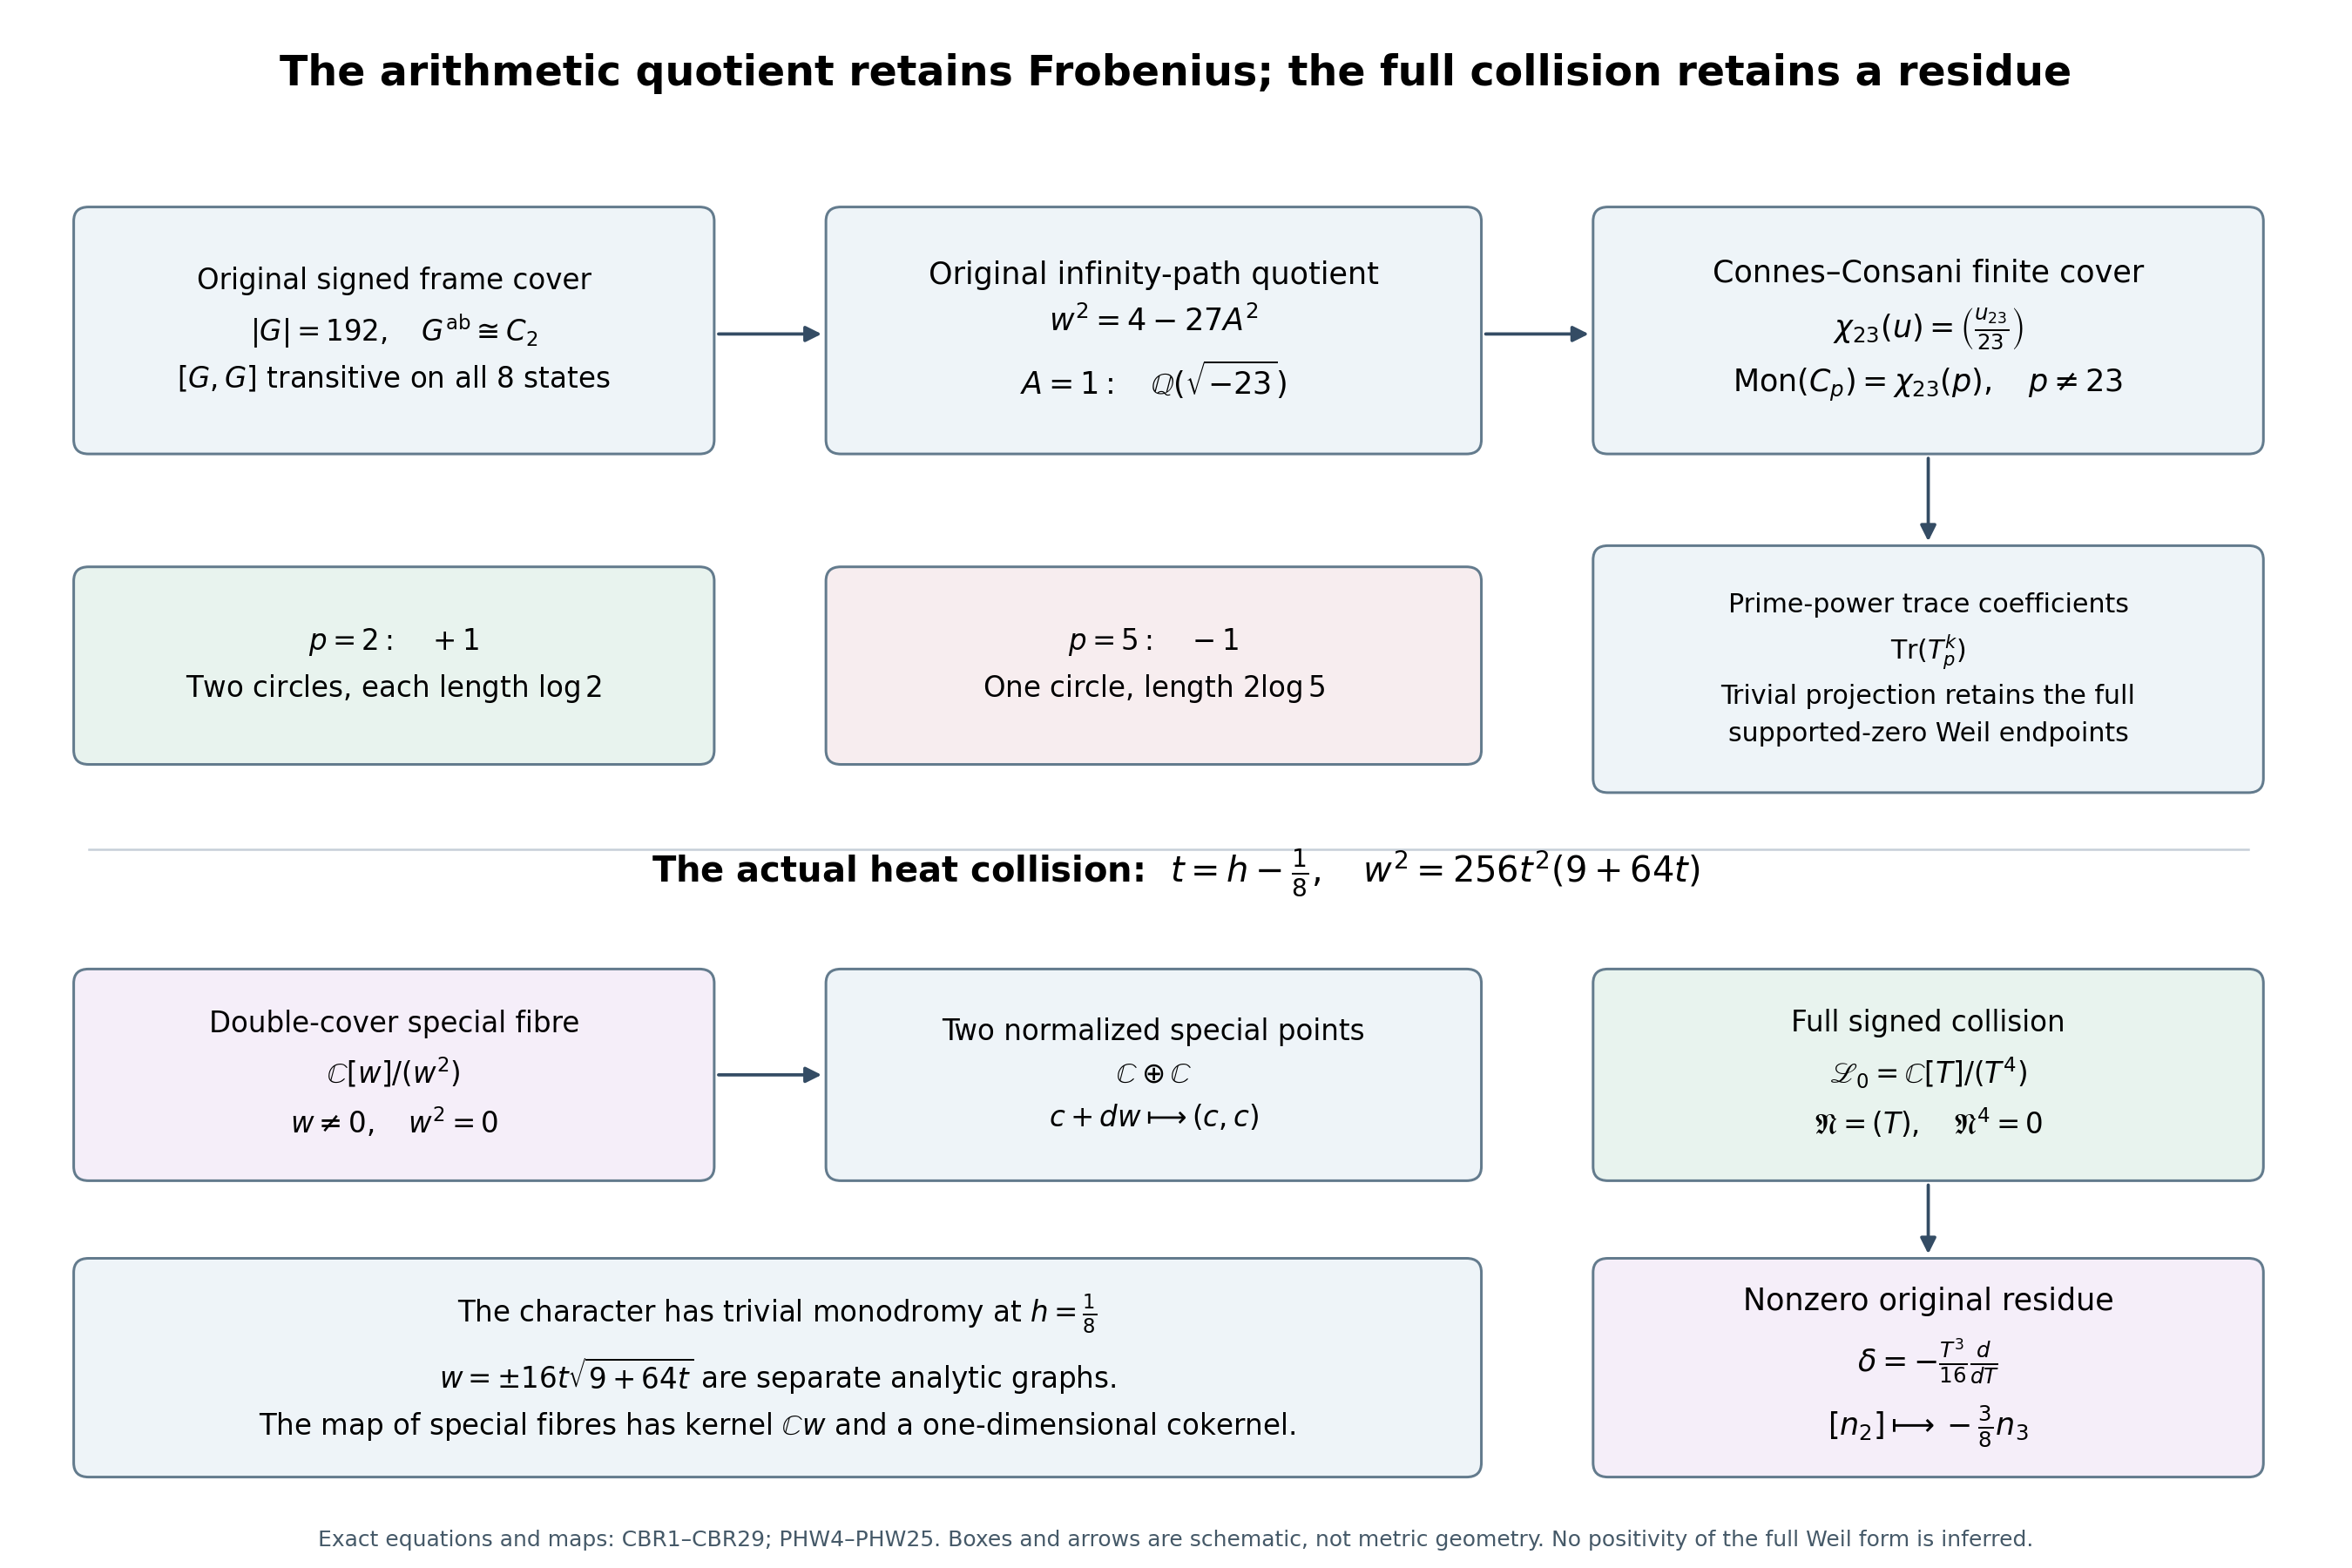
\includegraphics[keepaspectratio,alt={The original frame-cover quotient, its arithmetic specialization and prime returns, the two different special-fibre maps, and the surviving holonomy residue. CBR1--CBR29 and PHW4--PHW25 prove these exact maps. The box arrangement is schematic.}]{figures/34_class_field_holonomy.png}}
\caption{The original frame-cover quotient, its arithmetic
specialization and prime returns, the two different special-fibre maps,
and the surviving holonomy residue. CBR1--CBR29 and PHW4--PHW25 prove
these exact maps. The box arrangement is schematic.}
\end{figure}

\clearpage

\section{The original supported-zero identity on the heat
semimodule}\label{the-original-supported-zero-identity-on-the-heat-semimodule}

\textbf{Original-zeta receiving calculation.} The working meromorphic
function is the original Riemann zeta, with its full Gamma/endpoints
multiplier and its full trivial-zero and pole divisor retained.
\href{FAITHFUL_THETA_COMPLETION_RETURN.md}{TF1--42} proves the original
labelled theta inverse and the actual heat-image defect.
\href{FAITHFUL_UNCOMPLETED_ZETA_HEAT.md}{UZ1--53} proves every
exceptional-point fibre, jet, original-zeta heat term and reflection
orientation.
\href{ORIGINAL_ZETA_COMPACT_WEIL_RECONSTRUCTION.md}{OZC1--48} rederives
the compact contour and interval operator directly from zeta, including
the left-cutoff Gamma boundary, and specifies exactly which compensated
pairing the bounds concern.
\href{ORIGINAL_ZETA_HEAT_CONTACT_RECONSTRUCTION.md}{OZH1--49} rederives
the actual meromorphic heat, rational signed trace, compact-test domain,
contact drift and full causal arithmetic variation. The raw full divisor
and the compensated Weil receiver are linked by their displayed
correction, not identified. In particular the fixed-test trivial-zero
sum converges exactly at translations at least 1/32 and equals the
earlier R term; at zero translation it requires the proved cutoff
compensation. \href{ORIGINAL_ZETA_CAUCHY_RECONSTRUCTION.md}{OZK1--38}
reconstructs the original signed Cauchy trace, its full Gamma
correction, resonant finite parts, every finite matrix and its index,
and the complete local heat jets. Its invertible map retains the raw
trace and correction separately. These complete receiving proofs govern
the interpretation of the retained auxiliary calculations below.

23 September 2026. The calculation is at the unlocalized supported-zero
object. It retains the original semilattice and its module fibres.
Supported zero is the multiplicative identity of the original singlet
algebra, and this fact is used below rather than replaced by a
localization argument.

Primary programme source: \emph{An Algebraic Structure Incorporating a
Z/1Z-Symmetric Element Adjoined to the Integers},
\href{supporting_sources/17555345_11.tex\#L1146}{original source,
theorem thm:structure\_A and proof, lines1146--1260}. The construction
and operation table are at lines578--625. The support-semimodule
calculation below is proved directly from those operations. The
\href{FULL_SUPPORT_RECONSTRUCTION_DERIVATION.md}{full support
reconstruction} gives the earlier complete module comparison. The heat
source is Rodgers--Tao,
\href{https://arxiv.org/abs/1801.05914v5}{arXiv:1801.05914v5},
introduction, equations \texttt{hoz}, \texttt{phidef}, \texttt{htdef}
and theorem \texttt{main}; the bound0.2 is Platt--Trudgian,
\href{https://arxiv.org/abs/2004.09765v1}{arXiv:2004.09765v1},
subsection \emph{The de Bruijn--Newman constant}, its displayed
corollary. These literature results are cited, not claimed as new proofs
here.

\subsection{1. Supported zero is already invertible on the original
singlet
algebra}\label{supported-zero-is-already-invertible-on-the-original-singlet-algebra}

Let R be a nonzero commutative unital ring. In \[
S=G(R)=\{\tau\}\sqcup R^\bullet,\qquad e=0_R^\bullet,
\tag{ZH1}
\] use the original operations \(a^\bullet+b^\bullet=(a+b)^\bullet\),
\(a^\bullet b^\bullet=(ab)^\bullet\), \(\tau+x=x\) and \(\tau x=\tau\).
On the original subobject \(A=\{\tau,e\}\), their complete tables are

{\def\LTcaptype{none} % do not increment counter
\begin{longtable}[]{@{}lll@{}}
\toprule\noalign{}
+ & \(\tau\) & \(e\) \\
\midrule\noalign{}
\endhead
\bottomrule\noalign{}
\endlastfoot
\(\tau\) & \(\tau\) & \(e\) \\
\(e\) & \(e\) & \(e\) \\
\end{longtable}
}

{\def\LTcaptype{none} % do not increment counter
\begin{longtable}[]{@{}lll@{}}
\toprule\noalign{}
multiplication & \(\tau\) & \(e\) \\
\midrule\noalign{}
\endhead
\bottomrule\noalign{}
\endlastfoot
\(\tau\) & \(\tau\) & \(\tau\) \\
\(e\) & \(\tau\) & \(e\) \\
\end{longtable}
}

They prove \[
0_A=\tau,\qquad 1_A=e,\qquad e^{-1}=e\text{ in }A.
\tag{ZH2}
\] Closure is in the tables; associativity, commutativity and
distributivity restrict from \(S\). Hence this is a unital semiring
already inside the original set, without any localization. The inclusion
\(i:A\to S\) preserves addition, multiplication and additive zero. It
takes \(1_A\) to \(e\), whereas \(1_S=1_R^\bullet\). The exact unital
retraction in the other direction is \[
r:S\to A,\qquad r(x)=ex,\qquad ri=\operatorname{id}_A.
\tag{ZH3}
\] Distributivity proves additivity; \((ex)(ey)=e^2xy=exy\) proves
multiplicativity; \(r(1_S)=e=1_A\). These identities retain both
original units and prove their comparison.

\subsection{2. The identity acts on the entire semilattice of supported
zeros}\label{the-identity-acts-on-the-entire-semilattice-of-supported-zeros}

Let \(M\) be any \(S\)-semimodule, with its global zero \(0_M\). Define
\[
L_M=eM,\qquad p_M:M\to L_M,\quad m\mapsto em,\qquad
i_M:L_M\hookrightarrow M.
\tag{ZH4}
\] The equations \(e^2=e\), \(e+e=e\), \(r^\bullet e=e\) show that
\(L_M\) is a join-semilattice with addition as join and bottom \(0_M\).
Both \(p_M\) and \(i_M\) are \(S\)-linear, where supported scalars act
identically on \(L_M\) and \(\tau\) sends it to bottom. Their exact
compositions are \[
p_Mi_M=\operatorname{id}_{L_M},\qquad
i_Mp_M=e\cdot(-):M\to M,\qquad
e|_{L_M}=\operatorname{id}_{L_M}.
\tag{ZH5}
\] For example \(p_M(r^\bullet m)=er^\bullet m=em=r^\bullet p_M(m)\),
and the \(\tau\) equation follows from the semimodule zero law.
Additivity is distributivity. The inclusion has the same scalar laws
since they are restricted from \(M\). This proves every assertion in
ZH4--ZH5. In particular the action of supported zero on \(L_M\) is
invertible, with inverse itself, while every label of \(L_M\) remains
present.

The exact adjunction is also explicit. Regard any join-semilattice \(L\)
with bottom as an \(S\)-semimodule \(J(L)\), with every supported scalar
acting as identity and \(\tau\) acting as bottom. For an \(S\)-linear
\(f:M\to J(L)\), \[
f(m)=e f(m)=f(em).
\tag{ZH6}
\] Its restriction \(g:L_M\to L\) preserves joins and bottom. Conversely
any such \(g\) gives the \(S\)-linear map \(gp_M\). The two
constructions are inverse, since \(p_M\) restricts to the identity. Thus
\[
\operatorname{Hom}_S(M,J(L))
\simeq\operatorname{Hom}_{\vee,\bot}(eM,L).
\tag{ZH7}
\] This proves the reflection onto the semilattice of supported zeros,
with its unit \(p_M\). The natural inclusion \(i_M\) is retained as
well.

The same functor is also right adjoint to \(J\). Indeed, for an
\(S\)-linear \(h:J(L)\to M\), one has
\(h(\lambda)=h(e\lambda)=eh(\lambda)\), so its image is in \(eM\). Its
unique factorization through \(i_M\) is a map preserving joins and
bottom; conversely every such map gives \(h\) by inclusion. Therefore \[
\operatorname{Hom}_S(J(L),M)
\simeq\operatorname{Hom}_{\vee,\bot}(L,eM).
\tag{ZH7a}
\] The two adjunctions and ZH5 give the exact unit and counit maps on
the original zero object. No quotient of the ambient scalar semiring is
needed for these identities.

For each \(\lambda\in L_M\) the fibre \(M_\lambda=\{m:em=\lambda\}\) is
an \(R\)-module with local zero \(\lambda\). The group identities are
\(m+\lambda=(1_S+e)m=m\), \(m+(-1_R)^\bullet m=em=\lambda\), and
\(e((-1_R)^\bullet m)=\lambda\). They give inverses and closure within
the fibre. Scalar distributivity and associativity restrict from \(M\).
For \(\lambda\le\mu\), the linear transition is \(m\mapsto m+\mu\), as
direct substitution proves. Thus \(p_M\) returns the actual local zero
of each separate module fibre, retaining their separate labels.

Every \(S\)-linear \(F:M\to N\) obeys \[
p_NF=(F|_{eM})p_M,\qquad
Fi_M=i_N(F|_{eM}).
\tag{ZH8}
\] Both are the identity \(F(em)=eF(m)\). If \(F\) is invertible, its
restriction to \(eM\) is invertible, with inverse the restriction of
\(F^{-1}\). That restriction can have nontrivial permutations of support
labels. The equations do not assert that the full operator or its action
on a module fibre is the identity.

\subsection{3. A specified function space on which the actual heat flow
is
invertible}\label{a-specified-function-space-on-which-the-actual-heat-flow-is-invertible}

Let \(V\) consist of even complex measurable functions \(q\) on
\(\mathbb R\), up to almost-everywhere equality, with \[
\|q\|_a:=\int_{\mathbb R}e^{a u^2}|q(u)|\,du<\infty
\quad\text{for every real }a>0.
\tag{ZH9}
\] For every real \(t\) define \[
U_tq(u)=e^{tu^2}q(u).
\tag{ZH10}
\] This is a linear map \(V\to V\): choose \(b>\max(a+t,0)\), then
\(\|U_tq\|_a\le\|q\|_b\). Its exact group laws are \[
U_tU_s=U_{t+s},\qquad U_t^{-1}=U_{-t},\qquad U_0=\operatorname{id}_V.
\tag{ZH11}
\] These follow by multiplying the displayed exponential functions. Each
inverse is on the same function space \(V\); no bounded inverse on an
unspecified Hilbert space is asserted.

The cosine transform \[
(\mathcal Cq)(z)=\int_0^\infty q(u)\cos(zu)\,du
\tag{ZH12}
\] is entire. On any compact set \(|z|\le B\), every fixed derivative is
bounded by \(\int_0^\infty |q(u)|u^k e^{Bu}\,du\), which is finite
because \(u^k e^{Bu}\le C_{a,B,k}e^{au^2}\). Dominated differentiation
proves entire dependence. It is injective on \(V\): twice its
restriction to real \(z\) is the Fourier transform of the even \(L^1\)
function \(q\). For completeness Fourier uniqueness follows by
multiplying that transform by \(e^{-\epsilon x^2}\), applying Fubini
with the Gaussian Fourier identity, and obtaining \(q*g_\epsilon=0\);
the Gaussian approximate identities converge to \(q\) in \(L^1\), so
\(q=0\). All integrals used in this argument are absolutely convergent.
Define \(F=\mathcal C(V)\) with its transported vector-space structure.
Then \[
T_t=\mathcal C U_t\mathcal C^{-1}:F\to F
\tag{ZH13}
\] is an actual linear automorphism with inverse \(T_{-t}\).
Differentiating ZH12 gives \(\partial_tT_tF=-\partial_z^2T_tF\).

Let \(\Phi\) be exactly the Rodgers--Tao kernel \[
\Phi(u)=\sum_{n\ge1}(2\pi^2n^4e^{9u}-3\pi n^2e^{5u})e^{-\pi n^2e^{4u}}.
\tag{ZH14}
\] The source proves its evenness by Poisson summation. For \(u\ge0\),
factoring half the leading exponential gives \[
|\Phi(u)|\le C e^{9u}e^{-(\pi/2)e^{4u}},
\tag{ZH15}
\] where \(C\) is bounded by the convergent sum of
\((2\pi^2n^4+3\pi n^2)e^{-(\pi/2)n^2}\). Evenness supplies the negative
half-line. This bound proves \(\Phi\in V\). Hence the actual family is
on this space: \[
H_t=\mathcal C U_t\Phi=T_tH_0,\qquad
H_0(z)=\tfrac18\xi(\tfrac12+iz/2).
\tag{ZH16}
\] Thus the actual heat evolution is invertible at time0 and at every
other real time on the explicitly defined space F. This is a calculation
of the operator, not an inference from whether its current function has
real zeros.

\subsection{4. Carrying that heat group through the unlocalized
split-zero
construction}\label{carrying-that-heat-group-through-the-unlocalized-split-zero-construction}

For any complex vector space \(W\), its split extension is \[
G(W)=\{\tau_W\}\sqcup W^\bullet,\qquad e_W=0_W^\bullet,
\tag{ZH17}
\] with supported vector addition inherited from \(W\), absent additive
identity \(\tau_W\), \(c^\bullet w^\bullet=(cw)^\bullet\), supported
scalars fixing \(\tau_W\), and \(\tau\) sending every vector to
\(\tau_W\). These laws make an \(S=G(\mathbb C)\)-semimodule by direct
use of vector-space distributivity, with the cases containing \(\tau\)
giving the global zero.

The exact lifted flow is \[
G(T_t)(w^\bullet)=(T_tw)^\bullet,\qquad
G(T_t)(\tau_W)=\tau_W,\qquad W=F.
\tag{ZH18}
\] It is \(S\)-linear, has inverse \(G(T_{-t})\), and satisfies \[
G(T_0)=\operatorname{id}_{G(F)},\qquad
G(T_t)|_{eG(F)}=\operatorname{id}_{\{\tau_F,e_F\}}\quad(t\in\mathbb R).
\tag{ZH19}
\] The second equation follows because each linear \(T_t\) sends \(0_F\)
to \(0_F\), and the first follows from \(T_0=\operatorname{id}\). On
this original zero semilattice, supported zero itself acts as the same
identity by ZH5. On a general module diagram, ZH8 retains all labels and
their induced maps rather than replacing them by this particular
two-label example.

Evaluation at \(z\) is the \(S\)-linear map \[
G(\operatorname{ev}_z):G(F)\to G(\mathbb C),\qquad
w^\bullet\mapsto w(z)^\bullet,\quad\tau_F\mapsto\tau.
\tag{ZH20}
\] Consequently \[
G(\operatorname{ev}_z)(H_t^\bullet)=e\iff H_t(z)=0.
\tag{ZH21}
\] This is the actual map from the evolving function to the supported
zero at which it vanishes. Invertibility of \(G(T_t)\) as an evolution
operator does not assert invertibility of any evaluation or make ZH21
vacuous.

There is a direct test on the Riemann family itself. Rodgers--Tao proves
\(\Lambda\ge0\), so \(H_{-1}\) has a nonreal zero. Platt--Trudgian
proves \(\Lambda\le0.2\), so every zero of \(H_{0.2}\) is real. Both are
related by the actual invertible map \(T_{1.2}\), and both induce the
identity on the zero semilattice in ZH19. Therefore neither
invertibility of the heat evolution nor the identity action of supported
zero determines real-rootedness. This uses two actual members of the
Riemann heat family.

At \(t=0\), ZH21 still asks exactly whether a nonreal \(z\) can evaluate
\(H_0^\bullet\) to \(e\). The preceding calculations preserve this
evaluation map and leave that value question undetermined.

\subsection{5. The actual infinitesimal residue survives the zero
identity}\label{the-actual-infinitesimal-residue-survives-the-zero-identity}

The previously computed complex collision algebra is
\(C_0=\mathbb C[T]/(T^4)\), with retained derivation \[
D(T)=-T^3/16,\qquad D(1)=D(T^2)=D(T^3)=0.
\tag{ZH22}
\] This is the residue in
\href{https://github.com/KokunoYumeto/zeta-function-research-reader/blob/4a4238afc992e77aee83b97d38a1a63d283f540c/workbenches/splitzero-tandem/branches/tau-zero-prime-positivity/CLASS_FIELD_SIGNED_HOLONOMY_DERIVATION.md}{CBR25--CBR29},
read in its specified original collision coordinate. It descends from
\(-T^3\partial_T/16\) because it sends \(T^4\) to \(-T^6/4\), in the
defining ideal. Its square is zero and its image \(\mathbb CT^3\) has
square zero. Consequently, for each \(a\in\mathbb C\), \[
V_a=\operatorname{id}_{C_0}+aD,\qquad V_aV_b=V_{a+b},\qquad V_a^{-1}=V_{-a}
\tag{ZH23}
\] are algebra automorphisms. Indeed the Leibniz rule and the zero
product of two \(D\)-images prove multiplicativity, and \(D^2=0\) proves
the group law. The value \(V_a(T)=T-aT^3/16\) differs from \(T\) for
\(a\ne0\). These are the automorphisms generated by the retained
residue; no equality of the parameter \(a\) with heat time \(t\) or with
a particular meridian is imposed.

Their lifts \(G(V_a)\) commute with \(p_{G(C_0)}\) and restrict to the
identity on the zero semilattice by ZH8. Thus the nonzero infinitesimal
action and the invertible identity action of \(e\) coexist in the actual
collision receiver. Supported-zero identity does not remove the
infinitesimal direction.

The exact positive-form consequence for these automorphisms is
computable. Fix \(a\ne0\) and \(N=aD\). A positive semidefinite
Hermitian form \(Q\) on \(C_0\) is invariant under \(V_a\) precisely
when \(\operatorname{im}D\) is in its radical. To prove necessity,
invariance and \(V_a^n=\operatorname{id}+nN\) give, for every integer
\(n\), \[
Q(v+nNv,v+nNv)=Q(v,v).
\tag{ZH24}
\] The coefficient of \(n^2\) is \(Q(Nv,Nv)\), hence zero. For a
positive semidefinite Hermitian form a vector of square zero is radical:
expand \(Q(x+zy,x+zy)\ge0\) for arbitrary complex \(z\) to force
\(Q(x,y)=0\) when \(Q(x,x)=0\). Thus \(Q(Nv,w)=0\) for all \(v,w\).
Conversely that condition makes the cross and quadratic terms vanish,
proving invariance. Such forms correspond bijectively, by pullback, to
positive semidefinite Hermitian forms on \(C_0/\mathbb CT^3\). The
quotient kernel \(\mathbb CT^3\) is retained as a specified nonzero
line; no positive definite invariant form exists on the full
four-dimensional space. This is an exact statement about the
residue-generated action. The following
\href{COLLISION_RESIDUE_DUALITY_DERIVATION.md}{residue-duality
calculation, RD18--RD31b}, gives its actual trace comparison and the
corresponding full Weil-packet map.

\subsection{6. The full supported Weil formula and its constant
decomposition}\label{the-full-supported-weil-formula-and-its-constant-decomposition}

The
\href{https://github.com/KokunoYumeto/zeta-function-research-reader/blob/4a4238afc992e77aee83b97d38a1a63d283f540c/workbenches/splitzero-tandem/branches/tau-zero-prime-positivity/SUPPORTED_ZERO_PRIME_WEIL_DERIVATION.md\#L355}{established
supported-zero Weil identity, SZW33--SZW35} retains every label: \[
\boldsymbol B_L-\boldsymbol Z_L=\boldsymbol D_L.
\tag{ZH25}
\] Its lower fixed-support terms occur explicitly on both
\(\boldsymbol B_L\) and \(\boldsymbol D_L\); its arithmetic divisor
receiver is \(\boldsymbol Z_L\). They are retained by the identity
\(e|_{eM}\). In particular, a real-valued function on the labelled zero
set can distinguish \(\tau\) from \(e\); it need not be an additive
semiring character. The complete coordinate comparison is recorded in
\href{supporting_proofs/TAU_HEAT_ZERO_LOCALIZATION_DERIVATION.md}{HZ25--HZ29
of the accompanying heat-specialization calculation}.

The pole part of \(\Lambda(s)\) is \(1/(s-1)-1/s\). Multiplication by
\(s(s-1)/2\) makes that term exactly \(1/2\), and the Rodgers--Tao
factor \(1/8\) makes it \(1/16\) in \(H_0\). Here \(\Lambda(s)\) denotes
the completed meromorphic zeta function, separately from the real de
Bruijn--Newman constant. ZH12 represents \(H_0\) as the Fourier
transform of the absolutely continuous even measure \((\Phi(u)/2)\,du\),
which has no atom at zero. In the enlarged finite-measure Fourier
representation, \[
\tfrac12\Phi(u)\,du
=\tfrac1{16}\delta_0+
\left(\tfrac12\Phi(u)\,du-\tfrac1{16}\delta_0\right).
\tag{ZH26}
\] This is the exact source of the decomposition
\(H_0=1/16+(H_0-1/16)\). The opposite atom in the remainder is retained.
Multiplication by \(e^{tu^2}\) fixes both atoms, so their cancellation
persists. A labelled endpoint contribution in the full supported theta
construction can be retained independently; its map to the unlabelled
\(\Phi\) measure has exactly the cancellation in ZH26.

The calculation therefore accepts the original invertibility of
supported zero on its singlet algebra and on the entire zero
semilattice, constructs the lifted invertible heat group through it, and
retains the actual nonzero infinitesimal residue. The supported-zero
identity occurs with both real and nonreal zeros in the actual heat
family. The undecided arithmetic value is still the complete evaluation
and divisor pairing at time0.

\subsection{Independent verification and
illustration}\label{independent-verification-and-illustration}

The complete ZH1--ZH26 calculation, including ZH7a, received an
independent mathematical review. No mathematical error was found. The
constant \(1/16\) and \(H_0-1/16\) individually lie outside the
weighted-function cosine image \(F\), by the Riemann--Lebesgue property,
while their sum \(H_0\) lies in \(F\). The enlarged measure
representation in ZH26 is the stated domain for their separate terms.

\begin{figure}
\centering
\pandocbounded{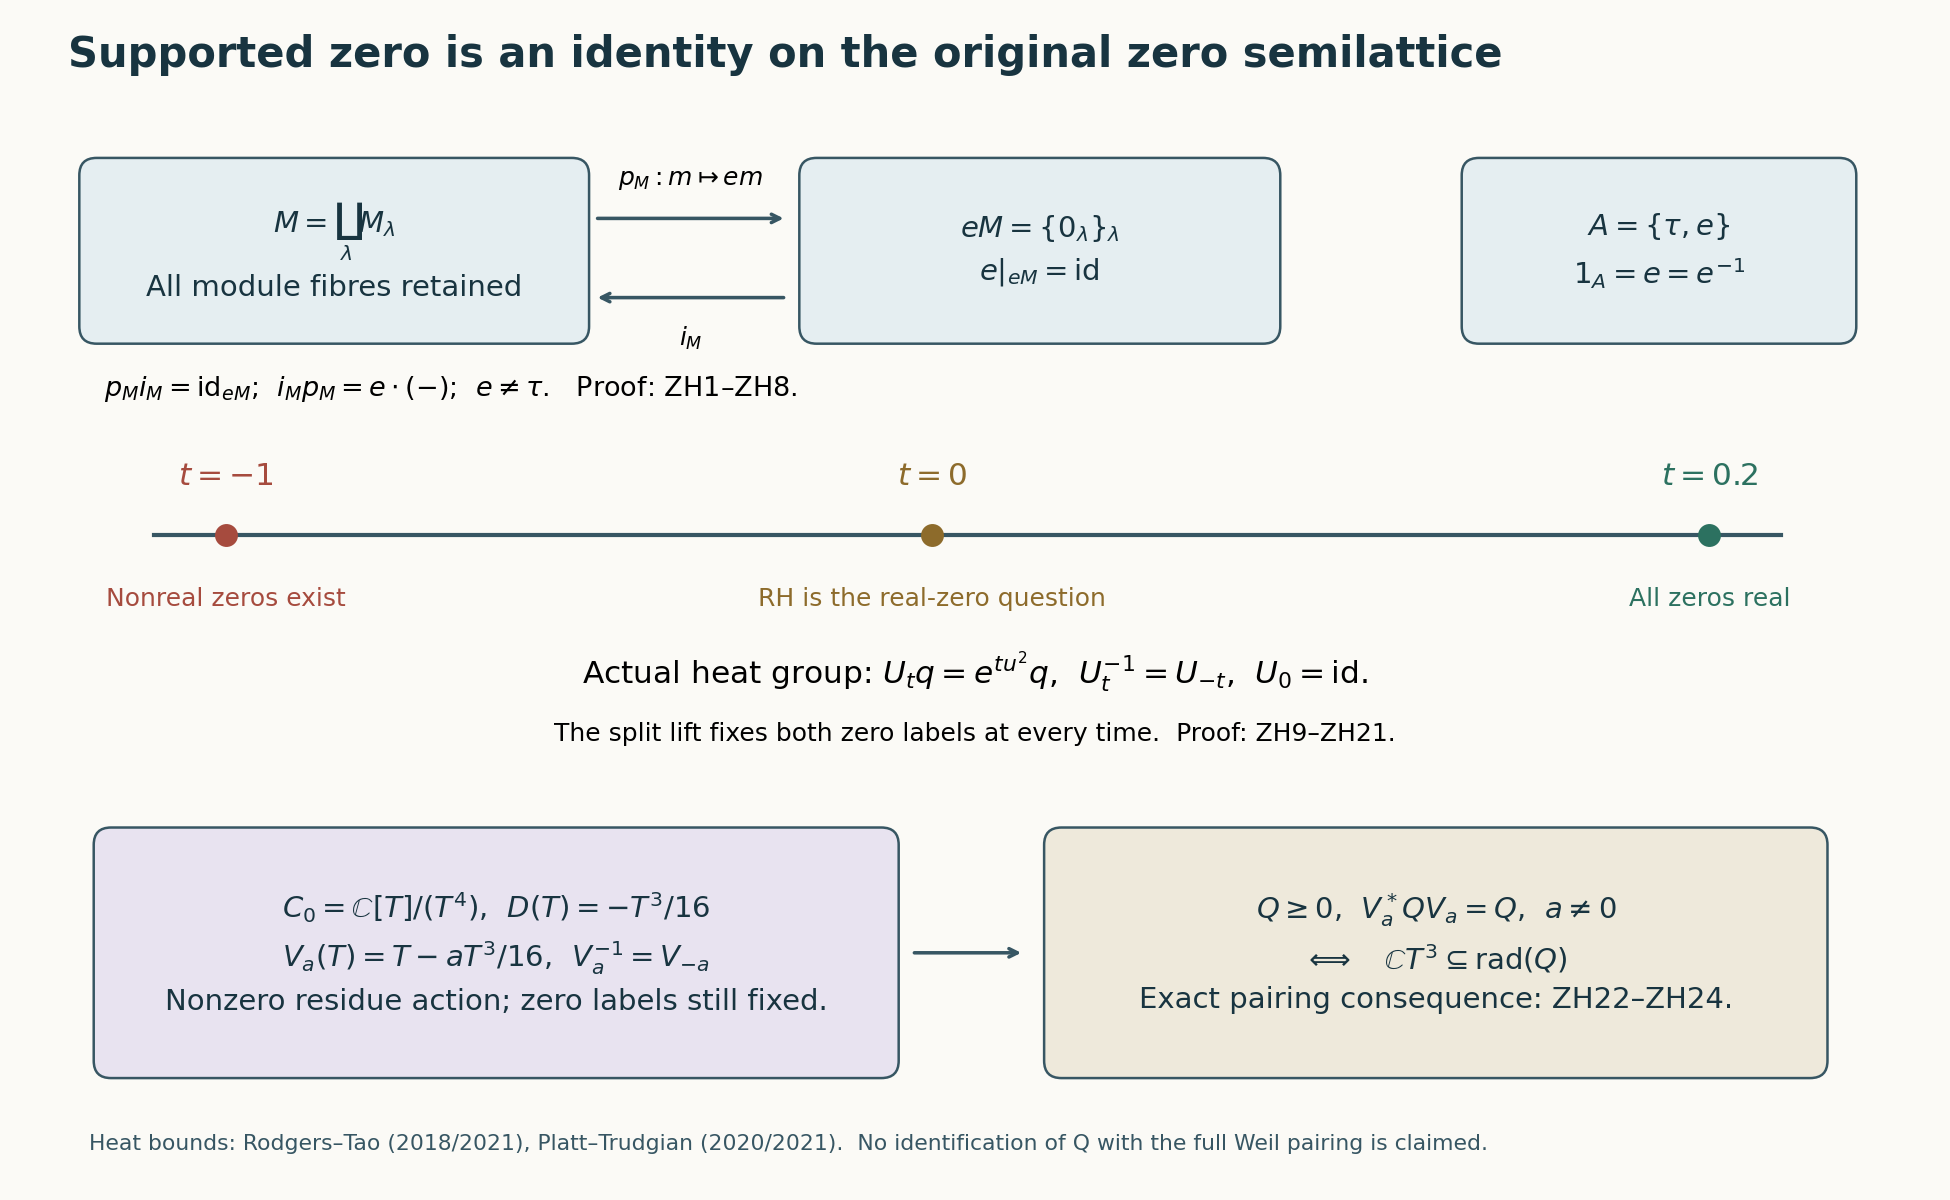
\includegraphics[keepaspectratio,alt={The original zero-semimodule retraction, the actual invertible heat evolution and its two known root regimes, and the exact invariant-form consequence of the retained residue. ZH1--ZH26 prove the displayed maps and statements. Time-marker positions are schematic and are not a numerical scale.}]{supported_zero_heat_identity.png}}
\caption{The original zero-semimodule retraction, the actual invertible
heat evolution and its two known root regimes, and the exact
invariant-form consequence of the retained residue. ZH1--ZH26 prove the
displayed maps and statements. Time-marker positions are schematic and
are not a numerical scale.}
\end{figure}

The reproducible figure source is
draw\_supported\_zero\_heat\_identity.py; both its PNG and SVG are
retained. The PNG was visually inspected. The two arrows at the top
preserve all module fibres and support labels; the lower arrow concerns
the residue-generated action, with no identification with an arithmetic
Weil pairing assumed.

\subsection{Actual global heat
continuation}\label{actual-global-heat-continuation-1}

The \href{ACTUAL_HEAT_ZERO_DISTRIBUTION_VARIATION.md}{global heat trace}
retains all zero multiplicities. The
\href{HEAT_CAUCHY_ARITHMETIC_DERIVATION.md}{arithmetic calculation,
HA1--HA26}, evaluates the complete supported formula on Cauchy tests and
computes its actual derivative. The local response keeps the complete
analytic unit; the global response includes mixed prime-product terms.
The \href{CAUCHY_WEIL_POSITIVITY_CRITERION.md}{matrix criterion} gives
the exact relation of this test family to RH. No sign from an isolated
local coefficient replaces the complete pairing.

\clearpage

\section{Residue duality, the collision Jacobian, and the supported Weil
trace}\label{residue-duality-the-collision-jacobian-and-the-supported-weil-trace}

23 September 2026.

This calculation gives the exact map from a perfect pairing that detects
the collision infinitesimal to the regular trace pairing that
annihilates it. It then proves the corresponding identity for the
programme's full Weil packets, including their original amplitude
multiplier and involution. The trace radical is identified with a
specified cotangent cohomology group. No off-critical zeta zero is
constructed, and no positivity of the full arithmetic form is asserted.

The incoming collision and meridian are
\href{https://github.com/KokunoYumeto/zeta-function-research-reader/blob/4a4238afc992e77aee83b97d38a1a63d283f540c/workbenches/splitzero-tandem/branches/tau-zero-prime-positivity/EIGHT_STATE_HOLONOMY_DERIVATION.md}{EHM43--EHM46}.
The incoming Weil multiplier and analytic identity are
\href{https://github.com/KokunoYumeto/zeta-function-research-reader/blob/4a4238afc992e77aee83b97d38a1a63d283f540c/workbenches/splitzero-tandem/branches/tau-zero-prime-positivity/WEIL_PACKET_DERIVATION.md}{WP13--WP46b}
and
\href{https://github.com/KokunoYumeto/zeta-function-research-reader/blob/4a4238afc992e77aee83b97d38a1a63d283f540c/workbenches/splitzero-tandem/branches/tau-zero-prime-positivity/WEIL_PACKET_ANALYTIC_DERIVATION.md}{WA24--WA30}.
The supported-zero identity used here is
\href{https://github.com/KokunoYumeto/zeta-function-research-reader/blob/4a4238afc992e77aee83b97d38a1a63d283f540c/workbenches/splitzero-tandem/branches/tau-zero-prime-positivity/SUPPORTED_ZERO_PRIME_WEIL_DERIVATION.md}{SZW33--SZW35}.
All additional finite algebra identities are proved below.

\subsection{1. The integral algebras and their complete duality
maps}\label{the-integral-algebras-and-their-complete-duality-maps}

Over the integers put \[
B=\mathbb Z[x,T]/(x^2(x+3),\,T^2-3x(x+2)),\qquad
C=\mathbb Z[\epsilon,T]/(\epsilon^2,\,T^2-6\epsilon).
\tag{RD1}
\] The original coordinate is \(x=R_{\rm original}-1\). First reducing
powers of \(T\), and then powers of \(x\), proves that the retained
bases are \[
\mathcal B_B=(1,x,x^2,T,xT,x^2T),\qquad
\mathcal B_C=(1,\epsilon,T,\epsilon T).
\tag{RD2}
\] Uniqueness follows by viewing \(B\) as the monic quadratic extension
of \(\mathbb Z[x]/(x^2(x+3))\), and \(C\) as the monic quadratic
extension of \(\mathbb Z[\epsilon]/(\epsilon^2)\). These are free of
ranks six and four. The surjective algebra map \[
q:B\longrightarrow C,\qquad q(x)=\epsilon,\quad q(T)=T
\tag{RD3}
\] is well defined: the first relation maps to zero and the second to
\(T^2-6\epsilon\). Its kernel is the free subgroup generated by
\(x^2,x^2T\), equivalently the ideal \((x^2)\). This follows directly
from RD2.

Define \(\lambda_B\) to be the coefficient of \(x^2T\), and
\(\lambda_C\) the coefficient of \(\epsilon T\). Their bilinear pairing
matrices \(\lambda(ab)\) in RD2 are \[
G_B=\begin{pmatrix}0&G\\G&0\end{pmatrix},
\quad
G=\begin{pmatrix}0&0&1\\0&1&-3\\1&-3&9\end{pmatrix},
\quad
G_C=\begin{pmatrix}0&0&0&1\\0&0&1&0\\0&1&0&0\\1&0&0&0\end{pmatrix}.
\tag{RD4}
\] For example \(x^3=-3x^2\) and \(x^4=9x^2\), which give every entry of
\(G\). A product with an even total power of \(T\) has no
\(T\)-coefficient, giving the two zero diagonal blocks. The analogous
calculations with \(\epsilon^2=0,T^2=6\epsilon\) give \(G_C\). In
particular \[
G^{-1}=\begin{pmatrix}0&3&1\\3&1&0\\1&0&0\end{pmatrix}.
\tag{RD5}
\] Thus both pairings are perfect over \(\mathbb Z\), not only over a
field. The maps \[
\Theta_B:B\xrightarrow{\sim}B^\vee,\quad
a\mapsto(f\mapsto\lambda_B(af)),\qquad
\Theta_C:C\xrightarrow{\sim}C^\vee
\tag{RD6}
\] are isomorphisms of modules over the respective algebras, where
\(A^\vee=\operatorname{Hom}_{\mathbb Z}(A,\mathbb Z)\) and
\((a\ell)(f)=\ell(af)\). This module assertion is immediate from
associativity. The inverse matrices in RD4--RD5 prove bijectivity
integrally.

For a finite free algebra \(A\), write
\(\operatorname{tr}_A(f)=\operatorname{Tr}(m_f)\), the regular
multiplication trace. If \(b_i,b_i^*\) are dual for \(\lambda\), then
the coefficient of \(b_i\) in \(fb_i\) is \(\lambda(b_i^*fb_i)\).
Summing the diagonal entries therefore gives \[
\operatorname{tr}_A(f)=\lambda\!\left(f\sum_i b_i b_i^*\right).
\tag{RD7}
\] For \(B\), the dual basis is \[
(3xT+x^2T,\;3T+xT,\;T,\;3x+x^2,\;3+x,\;1).
\] Its product sum is \(6x(x+2)T\). For \(C\), the dual basis is
\((\epsilon T,T,\epsilon,1)\), with product sum \(4\epsilon T\). These
are exactly the two Jacobian determinants: \[
J_B=\det\begin{pmatrix}3x(x+2)&-6(x+1)\\0&2T\end{pmatrix}
=6x(x+2)T,\qquad
J_C=\det\begin{pmatrix}2\epsilon&-6\\0&2T\end{pmatrix}
=4\epsilon T.
\tag{RD8}
\] Columns here are the differentials of the two defining relations, and
rows are \(dx,dT\), or \(d\epsilon,dT\). Consequently the full trace
maps are \[
\operatorname{tr}_B(f)=\lambda_B(J_Bf),\qquad
\operatorname{tr}_C(f)=\lambda_C(J_Cf).
\tag{RD9}
\] For \(f=p_0+p_1x+p_2x^2+(q_0+q_1x+q_2x^2)T\), the first equals
\(6p_0-6p_1+18p_2\). The second trace, for
\(f=a+b\epsilon+cT+d\epsilon T\), equals \(4a\). These formulas also
follow by direct multiplication matrices and hold after every base
change.

The dual of RD3 is particularly informative: \[
q^\vee\lambda_C=(x+3)\lambda_B,\qquad
q^\vee(c\lambda_C)=(x+3)\widetilde c\,\lambda_B.
\tag{RD10}
\] Here \(\widetilde c\) is any lift of \(c\). Indeed the coefficient of
\(x^2T\) in \((x+3)f\) is \(q_1\), because \(x^3+3x^2=0\); this equals
\(\lambda_C(qf)\). Independence of the lift follows from \((x+3)x^2=0\).
Thus RD10 proves the complete dual comparison, not just an equality of
dimensions. On traces it gives the exact decomposition \[
J_B=4x(x+3)T+2x^2T,\qquad
q^\vee\operatorname{tr}_C=4x(x+3)T\,\lambda_B.
\tag{RD11}
\] The two trace functionals evaluate to \(4p_0\) and
\(2(p_0-3p_1+9p_2)\). This formula holds over \(\mathbb Z\), including
at the prime three. It is not a claim that the integral algebra splits
as a direct product.

\subsection{2. The nonzero residue acts on perfect
duality}\label{the-nonzero-residue-acts-on-perfect-duality}

Base change now to \(\mathbb Z[1/2]\). Put \[
n_1=x(x+3),\quad n_3=Tx(x+3),\qquad
D_B(x)=0,\quad D_B(T)=-n_3/8,\qquad
D_C(\epsilon)=0,\quad D_C(T)=-3\epsilon T/8.
\tag{RD12}
\] The derivations descend: \(D_B(x^2(x+3))=0\), and the derivative of
the second relation is \(-T^2n_1/4=0\), since
\(T^2n_1=3x^2(x+2)(x+3)=0\). For \(C\) the only further check is
\(2TD_C(T)=-3\epsilon T^2/4=0\). Direct substitution gives
\(qD_B=D_Cq\). Also \(n_1^2=0\), \(D_B(n_1)=0\), and
\(\epsilon^2=D_C(\epsilon)=0\), proving \(D_B^2=D_C^2=0\).

For either algebra let \(D^\vee\ell=-\ell\circ D\). Then \[
D_B^\vee\lambda_B=\frac{n_1}{8}\lambda_B,\qquad
D_C^\vee\lambda_C=\frac{3\epsilon}{8}\lambda_C.
\tag{RD13}
\] For the general element \(f\) in RD9, \(D_Bf=-q_0n_3/8\): multiplying
\(n_3\) by \(x\) gives zero. Hence \(-\lambda_B(D_Bf)=q_0/8\), while
\(\lambda_B(n_1f)=q_0\), proving the first identity. The calculation on
the four coefficients of \(C\) gives the second. For an arbitrary
multiplier \(a\), the Leibniz rule proves the full connection formula \[
D^\vee(a\lambda)=(Da+ra)\lambda,\qquad
r_B=n_1/8,\quad r_C=3\epsilon/8.
\tag{RD14}
\] Indeed \(-\lambda(aDf)=-\lambda(D(af))+\lambda((Da)f)\). This is the
dual action on the specified dualizing module, not a Frobenius lift.
Compatibility with \(q^\vee\) follows both from \(qD_B=D_Cq\) and the
exact identity \((x+3)n_1=3n_1\).

The residue acts nontrivially on the perfect dual generators, but \[
D_BJ_B=0,\quad r_BJ_B=0,\qquad
D_CJ_C=0,\quad r_CJ_C=0.
\tag{RD15}
\] Each assertion follows by inserting RD8 into RD12--RD13 and using
\(x^2(x+3)=0\) or \(\epsilon^2=0\). Thus the two regular trace
functionals are fixed by the dual action. RD9 and RD13--RD15 identify
the precise map at which the nonzero action disappears.

\subsection{3. The complete Hermitian calculation on the complex
collision}\label{the-complete-hermitian-calculation-on-the-complex-collision}

After base change to \(\mathbb C\), there is the explicit isomorphism \[
C_{\mathbb C}\simeq C_0:=\mathbb C[T]/(T^4),\qquad
\epsilon\longmapsto T^2/6.
\tag{RD16}
\] Its inverse sends \(T\) to \(T\); \(T^4=36\epsilon^2=0\). This
isomorphism does not hold over \(\mathbb Z\): the natural map
\(\mathbb Z[T]/(T^4)\to C\) has image generated by
\(1,T,6\epsilon,6\epsilon T\), and cokernel \((\mathbb Z/6)^2\) on the
\(\epsilon\) and \(\epsilon T\) coordinates.

Use \(f^*(T)=\overline{f(-\overline T)}\), and define
\(\ell(f)=[T^3]f\). Then \(\ell(f^*)=-\overline{\ell(f)}\), so \[
Q_{\rm res}(f,g)=i\ell(f^*g)
\tag{RD17}
\] is Hermitian. Its matrix in \((1,T,T^2,T^3)\) has antidiagonal
entries \(i,-i,i,-i\), all other entries zero. Each of the pairs
\((1,T^3)\) and \((T,T^2)\) has one positive and one negative
eigenvalue, of absolute value one. Thus the form is nondegenerate with
inertia \((2,2,0)\).

The regular trace pairing and its exact comparison are \[
Q_{\rm tr}(f,g)=\operatorname{Tr}(m_{f^*g})=4\overline{f_0}g_0
=Q_{\rm res}(f,Kg),\qquad K=-4iM_{T^3}.
\tag{RD18}
\] The final equality follows by taking the coefficient of \(T^3\). The
multiplier \(-4iT^3\) is fixed by \(*\), so \(K\) is self-adjoint for
\(Q_{\rm res}\). It satisfies \[
K^2=0,\qquad \ker K=(T),\qquad \operatorname{im}K=\mathbb CT^3.
\tag{RD19}
\] The trace form is positive semidefinite with radical \((T)\). These
properties coexist with the indefinite, perfect residue form. They are
related by the displayed map; they are not contradictory positivity
claims about a single pairing.

All constants agree with the integral calculation. Under RD16,
\(\lambda_C=6\ell\) and \(J_C=(2/3)T^3\). Their product is
\(4\ell(T^3\,\cdot)\), exactly RD18.

The retained infinitesimal is \(D(T)=-T^3/16\), so \(Df=-f_1T^3/16\).
The maps \(V_a=1+aD\), for real \(a\), are algebra automorphisms:
\(D^2=0\) and \((Df)(Dg)=0\) show multiplicativity and
\(V_aV_b=V_{a+b}\). Their entire effect on RD17 is \[
Q_{\rm res}(V_af,V_ag)-Q_{\rm res}(f,g)
=-\frac{ia}{16}(\overline{f_0}g_1-\overline{f_1}g_0).
\tag{RD20}
\] Expanding the two factors proves this equality; the quadratic term is
zero because it contains \(T^6\). For \(a\ne0\) the difference has
inertia \((1,1,2)\), with nonzero eigenvalues \(\pm |a|/16\). Congruence
by the invertible \(V_a\) leaves the full residue form's inertia
\((2,2,0)\). The difference of the trace pairings is identically zero,
since \(V_a\) preserves \(f_0\).

This is a nonzero signed response to the infinitesimal, together with an
exact zero response after RD18. The \(V_a\) are the automorphisms
generated by the already computed residue. They are not identified with
the original finite-order meridian or with a new value of the original
heat clock.

\subsection{4. A complete monic-polynomial
identity}\label{a-complete-monic-polynomial-identity}

Let \(h(s)\) be any monic complex polynomial of degree \(n\ge1\), let
\(E_h=\mathbb C[s]/(h)\), and let \(\lambda_h(f)\) be the coefficient of
\(s^{n-1}\) in the remainder of \(f\) modulo \(h\). The bilinear form
\(\lambda_h(fg)\) is perfect: its matrix in \(1,s,\ldots,s^{n-1}\) is
zero when the row and column indices sum to less than \(n-1\), and is
one when they sum to \(n-1\). Reversing the columns gives a triangular
matrix with diagonal entries one. This proves invertibility without any
hypothesis on repeated roots.

The exact identity for every such polynomial is \[
\operatorname{Tr}_{E_h}(m_f)=\lambda_h(h'f).
\tag{RD21}
\] Here is a proof including the repeated-root case. For a polynomial
with distinct roots \(\alpha_j\), Lagrange interpolation of the
remainder \(r\) gives \[
\lambda_h(r)=\sum_j\frac{r(\alpha_j)}{h'(\alpha_j)}.
\] Apply this to the remainder of \(h'f\); the result is
\(\sum_jf(\alpha_j)\). Evaluation is an algebra isomorphism to
\(\mathbb C^n\), so this is also the regular trace. For each of the
basis choices \(f=1,s,\ldots,s^{n-1}\), both sides of RD21 are
polynomial expressions in the \(n\) coefficients of the monic \(h\): the
multiplication matrices and all remainders are obtained by monic
polynomial division. Their difference vanishes when the discriminant is
nonzero. A polynomial vanishing on that nonempty open subset of
\(\mathbb C^n\) is identically zero, for instance by the identity
theorem successively in each variable. Hence RD21 holds for every monic
\(h\), including all multiplicities. Linearity then proves it for all
\(f\in E_h\).

Suppose now that \(n\) is even and \(h^\#=h\), where \[
f^\#(s)=\overline{f(1-\overline s)}.
\tag{RD22}
\] This involution preserves \((h)\). A representative of degree less
than \(n\) remains of degree less than \(n\) after reflection, and its
top coefficient changes by \((-1)^{n-1}=-1\) and conjugation. Thus
\(\lambda_h(f^\#)=-\overline{\lambda_h(f)}\). It follows exactly as in
RD17 that \[
Q_h(f,g)=i\lambda_h(f^\#g)
\tag{RD23}
\] is a nondegenerate Hermitian form. Differentiating \(h^\#=h\) yields
\((h')^\#=-h'\), so \[
K_h=-iM_{h'},\qquad
Q_h(f,K_hg)=\operatorname{Tr}(m_{f^\#g}).
\tag{RD24}
\] The multiplier \(-ih'\) is fixed by \(\#\), proving its
self-adjointness for \(Q_h\). The factor \(h'\), rather than a freely
chosen positive metric, is forced by the trace identity RD21.

\subsection{5. The actual amplitude and the cotangent group of the Weil
packet}\label{the-actual-amplitude-and-the-cotangent-group-of-the-weil-packet}

Use the programme's \(g=2\xi\), the original \(s\)-coordinate, and its
finite involution-stable divisor \(h=d^m\), where \(d\) has four
distinct roots. The full quotient \(v_h=g/h\) is entire and nonzero at
those roots, because \(m\) is their exact multiplicity. Let \[
u=j_h(v_h)\in E_h,\qquad U=M_u.
\tag{RD25}
\] The remainder \(j_h\) is defined by simultaneous Taylor interpolation
through order \(m-1\) at each of the four roots. The Chinese remainder
theorem constructs it uniquely modulo \(h\), and its kernel is the
entire functions divisible by \(h\). Since each constant Taylor
coefficient of \(v_h\) is nonzero, its inverse in each truncated Taylor
algebra is the finite geometric-series inverse; therefore \(u\) and
\(U\) are invertible. All derivatives of \(v_h\) through the retained
orders occur in \(U\). None is replaced by its constant value in RD25.

The original packet pairing WP28 equals \[
B_h(f,g)=\operatorname{Tr}_{E_h}(m_{(uf)^\#(ug)})
=\lambda_h(h'u^\#u\,f^\#g)
=Q_h(Uf,K_hUg).
\tag{RD26}
\] To prove the first identity, in the primary factor at \(\alpha\) a
multiplication matrix is triangular with diagonal its constant
coefficient repeated \(m\) times. That coefficient here is
\(\overline{v_h(1-\overline\alpha)f(1-\overline\alpha)}v_h(\alpha)g(\alpha)\).
Summing over the four factors gives precisely WP28. The next two
equalities are RD21 and RD24. In particular all the amplitude factors,
the factor \(m\), and the sign in the reflected jets are retained.

The complete cotangent complex of this hypersurface over \(\mathbb C\)
has the presentation \[
L_{E_h/\mathbb C}=
\bigl[E_h\xrightarrow{\;h'\;}E_h\,ds\bigr],
\quad\text{in degrees }-1,0.
\tag{RD27}
\] One construction is the free differential graded resolution with
degree-zero generator \(s\) and degree-minus-one exterior generator
\(\eta\), differential \(d\eta=h(s)\). Its only underlying two terms are
multiplication by \(h\) on \(\mathbb C[s]\); this is injective and has
cokernel \(E_h\), so it resolves \(E_h\). Taking its differentials and
tensoring with \(E_h\) gives \(d\eta\mapsto h'ds\), proving RD27. Thus
its degree-minus-one cohomology is the explicitly included submodule
\(\operatorname{Ann}_{E_h}(h')\) of \(E_h\).

The precise comparison is \[
\operatorname{rad}B_h=\ker K_h
=\operatorname{Ann}_{E_h}(h')
=\frac{(d)}{(d^m)}
=H^{-1}(L_{E_h/\mathbb C}).
\tag{RD28}
\] For the radical equality, RD26 and perfection of \(\lambda_h\) show
that the radical in the second argument is
\(\operatorname{Ann}(h'u^\#u)\). The factor \(u^\#u\) is a unit, so this
is \(\operatorname{Ann}(h')\). Hermitian symmetry gives the same radical
in the first argument. Since \(h'=m d^{m-1}d'\) and \(d\) is squarefree
in characteristic zero, \(d'\) is relatively prime to \(d\);
cancellation in \(\mathbb C[s]\) proves that \(d^m\) divides \(h'f\)
exactly when \(d\) divides \(f\). This proves the middle ideal equality.
At \(m=1\) the displayed ideal is zero, as it should be.

Every map in RD28 is specified: a cohomology class represented by
\(a\eta\) maps to \(a\in E_h\); the radical inclusion is this same map.
The trace-to-dual map is \(\Theta_h\circ M_{h'}\), where
\(\Theta_h(a)(f)=\lambda_h(af)\). Multiplication by \(u^\#u\) gives the
amplitude-weighted version, with the same kernel. Its image has
dimension four, while its kernel and cokernel both have dimension
\(4m-4\). These dimensions follow from RD28 and the perfect
\(4m\)-dimensional duality, without discarding the kernel.

More precisely \(\operatorname{im}K_h=(d^{m-1})/(d^m)\), because
\(m d'\) is a unit modulo \(d^m\). For \(m\ge2\), \(2m-2\ge m\) shows
\(K_h^2=0\). For \(m=1\), \(K_h\) is invertible. In the off-critical
quartet, each reflected pair of primary summands is isotropic for
\(Q_h\), and they pair perfectly with each other. A dual basis for that
pairing gives a Hermitian block
\(\begin{pmatrix}0&I_m\\I_m&0\end{pmatrix}\), with inertia \((m,m,0)\).
The two reflected pairs therefore give inertia \((2m,2m,0)\) for the
full residue form. This retains the precise difference between the
perfect form and its rank-four trace image.

This identifies the surviving nilpotent packet directions with a
cotangent cohomology group through the trace's actual Jacobian. It does
not identify the whole collision algebra \(C_0\) with an arbitrary
actual zeta packet: their specified presentations and multiplicities
remain part of the comparison.

The other cotangent cohomology group is also retained: \[
H^0(L_{E_h/\mathbb C})=(E_h/(h'))\,ds,\qquad
H^{-1}(L_{E_h/\mathbb C})\times H^0(L_{E_h/\mathbb C})
\longrightarrow\mathbb C,\quad (a\eta,[b\,ds])\longmapsto\lambda_h(ab).
\tag{RD28a}
\] This pairing is well defined because \(ah'=0\). It is perfect:
multiplication by \(h'\) is self-adjoint for the perfect bilinear form
\(\lambda_h(ab)\), by commutativity. Therefore the orthogonal complement
of its image is its kernel. Identifying \(E_h\) with its dual by this
form identifies that kernel with the dual of its cokernel. This proves
both nondegeneracy assertions and supplies the exact duality map. For
\(m>1\) these two groups have dimension \(4m-4\); for \(m=1\) both are
zero. Thus the radical invisible to the regular trace is still detected
by an explicit pairing with the cotangent cokernel.

\subsection{6. The supported-zero formula keeps its endpoint
terms}\label{the-supported-zero-formula-keeps-its-endpoint-terms}

Retain the finite support semilattice \(L\), its top \(1_L\), and its
separate coordinate vectors \(\mathbf e_\lambda\). For an admissible
test with Mellin transform \(A(s)\), write \(P(A)\) and \(A_\infty(A)\)
for exactly the convergent finite-prime and archimedean terms of SZW24,
or their proved extension WA24. The full supported formula is \[
\begin{aligned}
\boldsymbol B_L(A)&=(A(0)+A(1))\mathbf e_{1_L}
+A(0)\sum_{\lambda\ne1_L}\mathbf e_\lambda,\\
\boldsymbol Z_L(A)&=Z(A)\mathbf e_{1_L},\\
\boldsymbol D_L(A)&=(P(A)-A_\infty(A))\mathbf e_{1_L}
+A(0)\sum_{\lambda\ne1_L}\mathbf e_\lambda,\\
\boldsymbol B_L(A)-\boldsymbol Z_L(A)&=\boldsymbol D_L(A).
\end{aligned}
\tag{RD29}
\] For the entire polynomial packet tests, take
\(A_{f,g}(s)=f^\#(s)g(s)v_h(s)^2\), with polynomial representatives
\(f,g\). The functional equation gives \(v_h^\#=v_h\), and WA24 proves
the full convergent analytic identity for these tests. All zeros outside
the chosen packet contribute zero because \(v_h\) vanishes there.
Therefore \[
\boldsymbol Z_L(A_{f,g})=
Q_h(U[f],K_hU[g])\,\mathbf e_{1_L}.
\tag{RD30}
\] The endpoint values in RD29 still use the actual entire function, not
merely its jet class.

Here is their exact behavior on a change in an invisible jet direction.
For a polynomial \(b\), replacing \(g\) by \(g+db\) changes its packet
class by \((d)/(d^m)\), and changes \(A\) by \(\Delta A=f^\#db\,v_h^2\).
Every packet value of \(\Delta A\) is zero, and the other zeros still
give zero. Thus \(\Delta Z=0\). Subtracting the two complete analytic
identities gives \[
\Delta(P-A_\infty)=\Delta A(0)+\Delta A(1),\qquad
\Delta\boldsymbol B_L=\Delta\boldsymbol D_L.
\tag{RD31}
\] The lower-label coordinates on both sides are exactly
\(\Delta A(0)\sum_{\lambda\ne1_L}\mathbf e_\lambda\). This proves the
compensation with every supported-zero term retained. It would be
incorrect to infer that the endpoints individually vanish because the
packet trace does.

There is an explicit nonzero endpoint witness. In the original quartet
write \(\rho=1/2+\delta+i\gamma\) and put \[
D_0=d(0)=d(1)=|\rho(1-\rho)|^2
=(1/4-\delta^2+\gamma^2)^2+4\delta^2\gamma^2>0.
\tag{RD31a}
\] The product formula for \(d\) proves the equalities. Since
\(2\xi(0)=2\xi(1)=1\), one has \(v_h(0)=v_h(1)=D_0^{-m}\). Taking
\(f=1,b=1\) in the preceding perturbation gives \[
\Delta A(0)=\Delta A(1)=D_0^{\,1-2m},\quad
\Delta(P-A_\infty)=2D_0^{\,1-2m},\quad \Delta Z=0.
\tag{RD31b}
\] Every lower support coordinate changes by the same positive number
\(D_0^{1-2m}\). This is an exact endpoint calculation on the programme
packet construction; it does not assert existence of an off-critical
zero. At \(m=1\) even the finite packet class is unchanged, while these
actual entire-test endpoint changes remain nonzero.

For completeness supported zero \(e\) remains the identity of
\(\{\tau,e\}\), with \(e^2=e\); the support projection on an
\(S\)-semimodule is \(p_M(m)=em\), with
\(p_Mi_M=\operatorname{id}_{eM}\). On the split extension of any algebra
above, a vanishing linear trace has value \(e\), while the unsupported
argument has value \(\tau\). The linear maps in RD9 lift by
\(f^\bullet\mapsto\operatorname{tr}(f)^\bullet\), \(\tau\mapsto\tau\).
The Hermitian pairings in RD18 and RD26 lift as sesquilinear maps: two
supported inputs give the bullet of their pairing, and an unsupported
input gives \(\tau\). No assertion of complex linearity of a Hermitian
first argument is intended. These formulas show precisely how a nonzero
algebra element can have supported trace zero without being identified
with the unsupported element.

The sign calculation remains exact. In an off-critical quartet the value
form is two blocks \(m\begin{pmatrix}0&1\\1&0\end{pmatrix}\), so it has
two positive and two negative directions, plus the \(4m-4\) radical
directions in RD28. The full endpoint expression equals that same value
form by RD29--RD30. This analysis does not establish the existence of an
off-critical quartet. It proves that modifying only its radical cannot
turn its negative value directions positive: for \(r\) in RD28,
\(B_h(f+r,f+r)=B_h(f,f)\). A proof of the desired arithmetic positivity
must therefore determine the sign on the retained value quotient; the
nonzero infinitesimal and its perfect residue pairing have now been
mapped to that exact question.

\subsection{7. Reproducible verification and
figure}\label{reproducible-verification-and-figure}

The accompanying exact symbolic checker verifies the integral duality
matrices, Jacobians, trace maps, quotient dual map, dual Lie weights,
and both complex Hermitian defects. The proofs above establish the
identities over their stated coefficient rings and for all monic
polynomials; finite checks are additional verification. The diagram
displays RD18--RD19 and RD26--RD31 with the full cotangent kernel
retained.

\begin{figure}
\centering
\pandocbounded{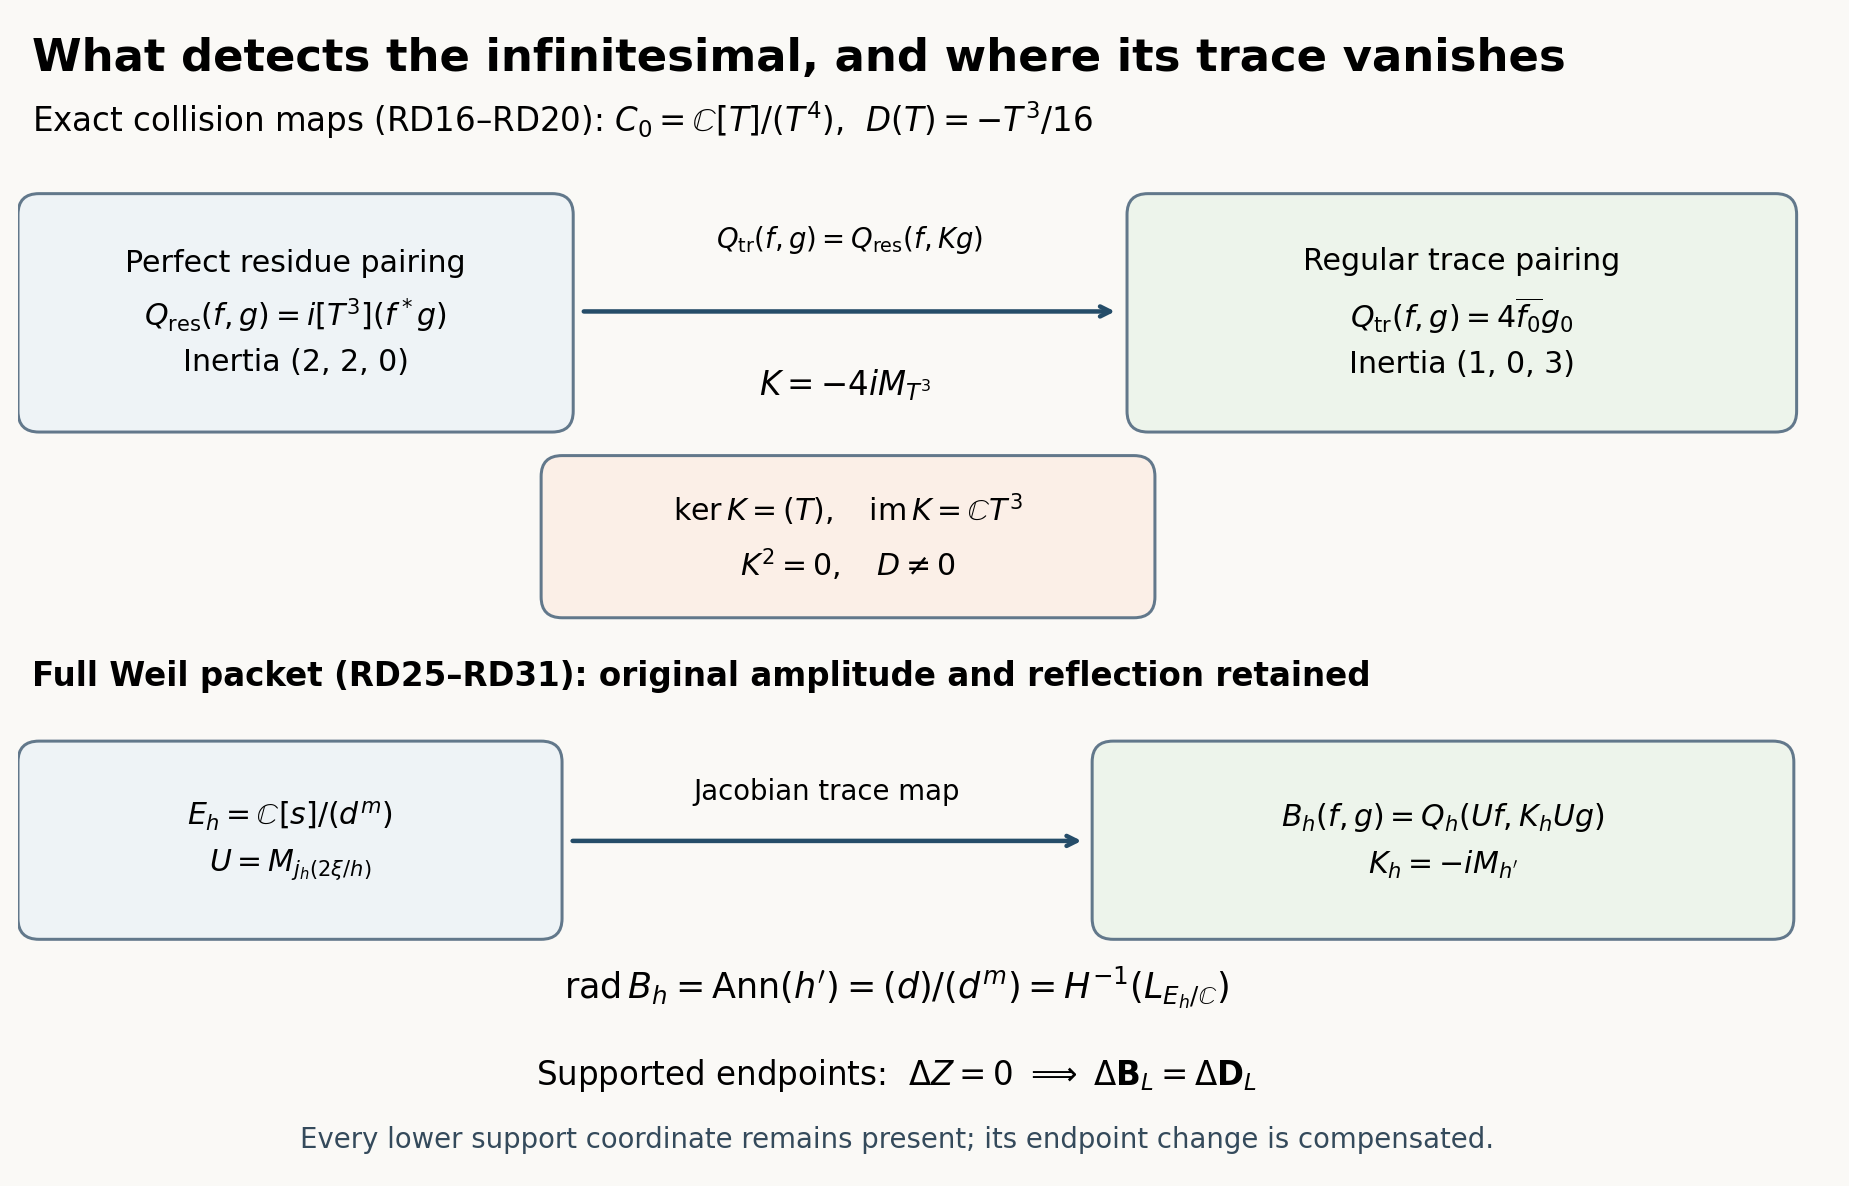
\includegraphics[keepaspectratio,alt={The Jacobian map from perfect residue duality to trace, and the retained supported endpoint terms.}]{collision_residue_duality.png}}
\caption{The Jacobian map from perfect residue duality to trace, and the
retained supported endpoint terms.}
\end{figure}

Figure: the upper row is the complex collision, with \(K=-4iM_{T^3}\),
kernel \((T)\), and image \(\mathbb CT^3\). The lower row is the actual
amplitude-weighted packet map, whose radical is RD28. The right-hand
equations retain the supported-zero boundary from RD29. This is a
diagram of proved linear maps and forms; it is not a plot of actual
off-critical zeta zeros.

\subsection{Integral prism
continuation}\label{integral-prism-continuation-1}

\href{DISTINGUISHED_COLLISION_PRISM_DERIVATION.md}{DP1--DP43} constructs
the specific bounded prism and proves the original nilradical
specialization.
\href{NILRADICAL_COTANGENT_EXTENSION_CLASS_DERIVATION.md}{EC1--EC48}
computes its complete extension class and the exact maps detecting the
divided residue.
\href{SUPPORTED_PRISM_SPECTRUM_DERIVATION.md}{SG1--SG23} gives the
supported prime pullbacks, retaining the unsupported point and the
original supported-zero prime under coefficient contraction. These
calculations retain all earlier trace and endpoint identities.

\subsection{Actual global heat
continuation}\label{actual-global-heat-continuation-2}

The \href{ACTUAL_HEAT_ZERO_DISTRIBUTION_VARIATION.md}{global heat trace}
retains all zero multiplicities. The
\href{HEAT_CAUCHY_ARITHMETIC_DERIVATION.md}{arithmetic calculation,
HA1--HA26}, evaluates the complete supported formula on Cauchy tests and
computes its actual derivative. The local response keeps the complete
analytic unit; the global response includes mixed prime-product terms.
The \href{CAUCHY_WEIL_POSITIVITY_CRITERION.md}{matrix criterion} gives
the exact relation of this test family to RH. No sign from an isolated
local coefficient replaces the complete pairing.

\clearpage

\section{The integral extension class, its connecting maps, and the
divided
residue}\label{the-integral-extension-class-its-connecting-maps-and-the-divided-residue}

Independent bounded derivation, 23 September 2026.

This proof continues
\href{https://github.com/KokunoYumeto/zeta-function-research-reader/blob/5a89872598df0902b7c1393cf8e4692ca3010a95/workbenches/splitzero-tandem/branches/tau-zero-prime-positivity/research_calculations/NILRADICAL_COTANGENT_DIVIDED_RESIDUE_DERIVATION.md}{NILRADICAL\_COTANGENT\_DIVIDED\_RESIDUE\_DERIVATION.md},
NC21--NC43. It computes the actual extension class over both
\(O=\mathbb Z_3\) and the original algebra \(C\), gives its connecting
maps, and relates its additional \(C\)-module data to the original
divided residue. The earlier source is unchanged.

\subsection{EC1. The retained extension and scalar
actions}\label{ec1.-the-retained-extension-and-scalar-actions}

Put \[
C=O[\epsilon,T]/(\epsilon^2,T^2-6\epsilon),\qquad
R=C/(3,\epsilon)=\mathbb F_3[T]/T^2.
\tag{EC1}
\] The original modules, here denoted \(N,E\), are \[
N=(O/3O)a\oplus(O/9O)b,\qquad
E=(O/9O)c_1\oplus(O/9O)c_2\oplus(O/3O)w.
\tag{EC2}
\] Their generator actions are \[
\epsilon a=0,\quad\epsilon b=-3b,\quad
Ta=-3b,\quad Tb=0;
\tag{EC3}
\] \[
\epsilon c_1=\epsilon c_2=0,\quad\epsilon w=3c_2,\qquad
Tc_1=c_2,\quad Tc_2=Tw=0.
\tag{EC4}
\] These actions respect the relations of \(C\). For example
\(T^2a=T^2b=0\), while \(6\epsilon b=-18b=0\); on \(E\), \(T^2\) is zero
and \(6\epsilon w=18c_2=0\). The two generator actions commute on every
displayed basis vector, and \(\epsilon^2=0\).

The exact sequence is \[
0\longrightarrow N\xrightarrow{\kappa}E\xrightarrow{\psi}R
\longrightarrow0,
\tag{EC5}
\] where \[
\kappa(a)=3c_1,\quad\kappa(b)=w-c_2,\qquad
\psi(c_1)=1,\quad\psi(c_2)=\psi(w)=T.
\tag{EC6}
\] The action tables prove \(C\)-linearity. In particular \[
T\kappa(a)=3c_2=\kappa(-3b),\qquad
\epsilon\kappa(b)=3c_2=\kappa(-3b).
\] The \(c_2\)-coordinate of \(\kappa(xa+yb)=0\) first forces \(y=0\)
modulo 9, and the \(c_1\)-coordinate then forces \(x=0\) modulo 3. Thus
\(\kappa\) is injective. The map \(\psi\) is onto, and its kernel
consists of \(c_1\)-coefficients divisible by 3 and pairs of
\(c_2,w\)-coefficients whose sum is zero modulo 3. These are exactly the
image of \(\kappa\).

Write \[
M=N[3]=\mathbb F_3a\oplus\mathbb F_3(3b),\qquad
3N=\mathbb F_3(3b).
\tag{EC7}
\] On all of \(N\), \(\epsilon=-3\,\mathrm{id}_N\). On \(M\),
\(\epsilon=0\), \(Ta=-3b\), and \(T(3b)=0\). Consequently \[
R\xrightarrow{\sim}M,\qquad 1\mapsto a,\quad T\mapsto-3b
\tag{EC8}
\] is a \(C\)-linear isomorphism. This fixes the signs of the later
connecting maps.

\subsection{EC2. The coefficient-3 connecting
map}\label{ec2.-the-coefficient-3-connecting-map}

For \(r\in R\), choose a lift \(h\in E\). Since \(3r=0\), the element
\(3h\) belongs to \(\kappa(N)\). Define \[
\beta:R\longrightarrow N/3N,\qquad
\beta(r)=[\kappa^{-1}(3h)].
\tag{EC9}
\] If \(h\) is changed to \(h+\kappa(n_0)\), the element inside brackets
changes by \(3n_0\). Thus the definition is independent of the lift.
Adding lifts and multiplying them by a scalar in \(C\) proves that
\(\beta\) is \(C\)-linear; in particular it is \(O\)-linear.

For the chosen lifts \(c_1,c_2\), \[
3c_1=\kappa(a),\qquad 3c_2=\kappa(-3b).
\] Hence \[
\boxed{\beta(1)=\overline a,\qquad\beta(T)=0.}
\tag{EC10}
\] Here \[
N/3N=\mathbb F_3\overline a\oplus\mathbb F_3\overline b,
\] and both \(\epsilon,T\) act as zero: their values on \(N\) lie in
\(3N\). Consequently the formula on \(T\) is also required by
\(C\)-linearity once \(\beta(1)\) has been fixed. The exact modules are
\[
\ker\beta=\mathbb F_3T,\quad
\operatorname{im}\beta=\mathbb F_3\overline a,\quad
\operatorname{coker}\beta=\mathbb F_3\overline b.
\tag{EC11}
\] All three are \(C\)-modules on which \(3,\epsilon,T\) act as zero.

This map is the connecting map in the full coefficient-3 sequence \[
0\to N[3]\to E[3]\to R
\xrightarrow{\beta}N/3N\to E/3E\to R\to0.
\tag{EC12}
\] One can obtain it by applying the kernel-cokernel sequence to
multiplication by 3 on EC5. There is also a direct verification of every
map. The groups are \[
E[3]=\mathbb F_3(3c_1)\oplus\mathbb F_3(3c_2)\oplus\mathbb F_3w,
\] \[
E/3E=\mathbb F_3\overline c_1\oplus
\mathbb F_3\overline c_2\oplus\mathbb F_3\overline w.
\] The first injection sends \[
a\mapsto3c_1,\qquad3b\mapsto-3c_2.
\] The next map sends \(w\mapsto T\) and kills \(3c_1,3c_2\), so its
image is the kernel of EC10. The map \(N/3N\to E/3E\) sends \[
\overline a\mapsto0,\qquad
\overline b\mapsto\overline w-\overline c_2.
\] Its kernel is precisely \(\operatorname{im}\beta\). Finally
\(E/3E\to R\) sends
\(\overline c_1\mapsto1,\overline c_2,\overline w\mapsto T\), and its
kernel is the line generated by \(\overline w-\overline c_2\). This
proves exactness of EC12 without leaving its maps implicit.

The actions in EC12 are retained. On \(E[3]\), \[
T(3c_1)=3c_2,\qquad\epsilon w=3c_2,
\] and all other actions of \(\epsilon,T\) on the indicated three
generators vanish. In particular \(\epsilon\) does not annihilate
\(E[3]\). On \(E/3E\), \(\epsilon=0\), \(T\overline c_1=\overline c_2\),
and \(T\overline c_2=T\overline w=0\). Each displayed map respects these
actions.

\subsection{\texorpdfstring{EC3. The exact class after forgetting to
\(O\)}{EC3. The exact class after forgetting to O}}\label{ec3.-the-exact-class-after-forgetting-to-o}

As an \(O\)-module, \(R\) has the free resolution \[
0\longrightarrow O^2\xrightarrow{3}O^2\longrightarrow R
\longrightarrow0,
\] where the final basis vectors map to \(1,T\). Applying
\(\operatorname{Hom}_O(-,N)\) gives \[
\operatorname{Ext}^1_O(R,N)
\simeq(N/3N)^2
\simeq\operatorname{Hom}_{\mathbb F_3}(R,N/3N)
\simeq\mathbb F_3^4.
\tag{EC13}
\] Explicitly, an extension is assigned the two values \(3h_1,3h_T\) in
\(N\), modulo \(3N\), for lifts of \(1,T\). Changing the lifts adds
multiples of 3. Conversely any pair of representatives
\(\alpha_1,\alpha_T\in N\) gives the extension \[
(N\oplus O h_1\oplus O h_T)/
(3h_1-\alpha_1,\;3h_T-\alpha_T).
\] Injection of \(N\) follows by comparing the two free coordinates in a
proposed relation. Two pairs differing by multiples of 3 give equivalent
extensions by changing their lifts. This proves EC13 as a classification
of extensions and identifies its class map with EC9.

Thus the underlying \(O\)-class of EC5 is the nonzero homomorphism \[
\varphi(1)=\overline a,\qquad\varphi(T)=0.
\tag{EC14}
\] It has order 3 in the extension group. The extension is therefore
nonsplit over \(O\). Directly, no lift of \(1\) can be killed by 3: its
\(c_1\)-coefficient is a unit modulo 3 and has nonzero triple modulo 9.

The full target in EC13 has dimension four. The forgetful map from
\(C\)-extensions below does not have this whole group as its image.

\subsection{\texorpdfstring{EC4. Presentation of the \(C\)-extension
group}{EC4. Presentation of the C-extension group}}\label{ec4.-presentation-of-the-c-extension-group}

Let \(I=(3,\epsilon)\subset C\), so \(R=C/I\). The map \[
C^2\longrightarrow I,\qquad (u,v)\longmapsto3u+\epsilon v
\] has kernel generated by \[
(\epsilon,-3),\qquad(0,\epsilon).
\tag{EC15}
\] To prove completeness of these syzygies, write
\(u=u_0+u_1\epsilon+u_2T+u_3\epsilon T\) and likewise for \(v\). Since
\(C\) is \(O\)-free on \(1,\epsilon,T,\epsilon T\), the equation
\(3u+\epsilon v=0\) gives \[
u_0=u_2=0,\qquad v_0=-3u_1,\qquad v_2=-3u_3.
\] It follows that \[
(u,v)=(u_1+u_3T)(\epsilon,-3)+(v_1+v_3T)(0,\epsilon).
\] This proves EC15 without dividing by 3 in \(C\).

Because \(C\) is a free module over itself, the sequence
\(0\to I\to C\to R\to0\) yields \[
\operatorname{Ext}^1_C(R,N)
\simeq
\frac{\operatorname{Hom}_C(I,N)}
{\{i\mapsto in_0:n_0\in N\}}.
\] A homomorphism \(F:I\to N\) is determined by \(n=F(3)\),
\(m=F(\epsilon)\). The syzygies give \[
\epsilon n=3m,\qquad\epsilon m=0.
\tag{EC16}
\] Write \(n=u a+y b\), \(m=u'a+z b\). Since \(\epsilon b=-3b\), the
second relation forces \(z\in3O/9O\), and the first then forces
\(y\in3O/9O\). Thus both \(n,m\) lie in \(M=N[3]\), and every pair in
\(M^2\) satisfies EC16. The restrictions from \(C\) are \[
(3n_0,\epsilon n_0)=(3n_0,-3n_0).
\] They form the one-dimensional subspace generated by \((3b,-3b)\).
Consequently \[
\boxed{\operatorname{Ext}^1_C(R,N)
=\frac{M\oplus M}{\mathbb F_3(3b,-3b)}
\simeq\mathbb F_3^3.}
\tag{EC17}
\]

Here is the exact extension associated to a pair \((n,m)\). Use the
homomorphism \(F\) just proved and form \[
E_{n,m}=(N\oplus C u)/\{(-F(i),iu):i\in I\}.
\tag{EC18}
\] Then \(N\to E_{n,m}\) is injective: if \((z,0)=(-F(i),iu)\), the free
\(C u\)-coordinate forces \(i=0\), hence \(z=0\). The quotient is
\(C/I=R\). The chosen lift \(u\) of \(1\) satisfies \[
3u=n,\qquad\epsilon u=m.
\tag{EC19}
\] Conversely a lift \(u\) in any \(C\)-extension defines \(F(i)=iu\)
and gives an isomorphism from EC18 to that extension, fixing both \(N\)
and \(R\). Changing \(u\) by \(n_0\in N\) changes its pair by
\((3n_0,\epsilon n_0)\). This proves the full equivalence relation, and
also shows that addition of pairs is the usual addition of extension
classes.

For EC5 the lift \(u=c_1\) gives \[
(n,m)=(a,0).
\tag{EC20}
\] Thus the actual class has been specified in the extension group, not
only tested for nonsplitting.

\subsection{\texorpdfstring{EC5. The full \(C\)-action and the invisible
nonzero
class}{EC5. The full C-action and the invisible nonzero class}}\label{ec5.-the-full-c-action-and-the-invisible-nonzero-class}

Set \[
E_1=[(a,0)],\qquad E_2=[(0,a)],\qquad
E_3=[(3b,0)]=[(0,3b)].
\tag{EC21}
\] The last equality is exactly the boundary in EC17. These form an
\(\mathbb F_3\)-basis. The \(C\)-action, defined by multiplication on
the target \(N\), is \[
TE_1=TE_2=-E_3,\qquad TE_3=0,\qquad
3E_j=\epsilon E_j=0.
\tag{EC22}
\] For example \(T(a,0)=(-3b,0)\), and \(T(0,a)=(0,-3b)\). These prove
every action in EC22.

Under forgetting to \(O\), the two underlying lifts are \(u,Tu\), so the
coefficient-3 class is \[
1\longmapsto[n],\qquad T\longmapsto[Tn]
\quad\text{in }N/3N.
\tag{EC23}
\] For \[
n=u a+3v b,\qquad m=u'a+3v'b
\quad(u,v,u',v'\in\mathbb F_3),
\] one has \(Tn=-3u b\), which lies in \(3N\). Therefore forgetting
sends \[
E_1\mapsto\varphi,\qquad E_2,E_3\mapsto0.
\tag{EC24}
\] Its exact image is the one-dimensional line \(\mathbb F_3\varphi\)
inside the four-dimensional group EC13; its kernel is
\(\mathbb F_3E_2\oplus\mathbb F_3E_3\), isomorphic to \(R\) by \[
1\mapsto E_2,\qquad T\mapsto-E_3.
\] The target \(C\)-action here is the one induced by multiplication on
\(N\). On \(N/3N\), both \(\epsilon,T\) act as zero, so the target in
EC13 is a trivial \(R\)-module. This specifies the action and proves
\(C\)-linearity of the forgetful map. Precomposition by multiplication
on \(R\) gives a separate action on the full group EC13; the two actions
agree on the image of \(C\)-extensions.

The exact kernel-image sequence of the forgetful map splits as
\(R\)-modules by \[
\varphi\longmapsto E_1-E_2,
\] because \(T(E_1-E_2)=0\). Thus \[
\operatorname{Ext}^1_C(R,N)
=R E_2\oplus\mathbb F_3(E_1-E_2)
\simeq R\oplus\mathbb F_3.
\tag{EC25}
\] This is a splitting of a sequence of extension groups. It is not a
splitting of EC5.

The actual class is \(E_1\), and \[
TE_1=-E_3\ne0.
\tag{EC26}
\] The underlying \(O\)-class of \(TE_1\) is zero by EC24. The
annihilator of \(E_1\) in \(C\) is exactly \((3,\epsilon)\): the action
factors through \(R\), and \(E_1,TE_1\) are independent over
\(\mathbb F_3\). Hence the cyclic module \(CE_1\) is isomorphic to
\(R\). The nonzero \(T\)-layer of this class is invisible after
forgetting \(C\).

There is a concrete presentation of this invisible class. For \(-E_3\),
take \[
3u=-3b,\qquad\epsilon u=0.
\] Changing the lift to \(u'=u+b\) gives \[
3u'=0,\qquad \epsilon u'=-3b.
\tag{EC27}
\] Then \(u',Tu'\) define an \(O\)-linear section of the quotient, since
both are killed by 3. A \(C\)-linear section would need a lift of \(1\)
killed by both 3 and \(\epsilon\). Any other lift killed by 3 differs
from \(u'\) by an element of \(M=N[3]\), and \(\epsilon M=0\); its
\(\epsilon\)-value is therefore still \(-3b\ne0\). This proves directly
that the same extension is split over \(O\) and nonsplit over \(C\).

\subsection{EC6. A canonical second connecting
map}\label{ec6.-a-canonical-second-connecting-map}

The scalar \(3+\epsilon\) annihilates both \(N\) and \(R\). Consequently
every extension
\(0\to N\xrightarrow{\kappa'}E'\xrightarrow{\psi'}R\to0\) has a
canonical \(C\)-linear map \[
\rho_{E'}:R\longrightarrow N,\qquad
\kappa'\rho_{E'}(r)=(3+\epsilon)h
\quad(\psi'h=r).
\tag{EC28}
\] The right side lies in the image of \(\kappa'\), since \(3+\epsilon\)
annihilates \(R\). It is independent of \(h\), since the same scalar
annihilates \(N\). These facts prove existence, uniqueness, and
\(C\)-linearity. Its image lies in \(M\), since \(R\) is killed by 3.
For the cocycle of EC19, \[
\rho_{E_{n,m}}(1)=n+m,\qquad
\rho_{E_{n,m}}(T)=T(n+m).
\tag{EC29}
\]

The two class data give the exact \(C\)-linear isomorphism \[
\boxed{
\operatorname{Ext}^1_C(R,N)
\xrightarrow{\sim}(M/3N)\oplus M,\qquad
[(n,m)]\longmapsto([n],n+m).}
\tag{EC30}
\] The boundary \((3n_0,-3n_0)\) changes neither coordinate. If both
coordinates vanish, \(n\in3N\) and \(m=-n\), so the pair is precisely a
boundary. Given \(([\alpha],z)\), choose \(\alpha\in M\) and take
\((n,m)=(\alpha,z-\alpha)\); changing \(\alpha\) by an element of \(3N\)
changes this pair by a boundary. This proves surjectivity and gives a
well-defined inverse. Componentwise scalar multiplication proves
\(C\)-linearity.

The first coordinate of EC30 is the entire possible underlying
\(O\)-class, interpreted by \(1\mapsto[n],T\mapsto0\). The second
coordinate specifies the whole map \(\rho\), since
\(\operatorname{Hom}_C(R,N)\simeq M\) by evaluation at 1. Thus this is a
classification by actual connecting maps.

For EC5, \[
\rho(1)=a,\qquad \rho(T)=-3b.
\tag{EC31}
\] In particular \(\rho:R\to M\) is the isomorphism EC8, and its class
coordinates in EC30 are \((\overline a,a)\). The class \(E_1-E_2\) has
the same underlying \(O\)-class but \(\rho=0\). Their difference \(E_2\)
is nonzero and invisible to forgetting. There are exactly nine
\(C\)-extension classes over each \(O\)-class in the image, because the
second summand \(M\) has nine elements.

For the actual extension, \(\beta\) is the reduction of \(\rho\) modulo
\(3N\): \[
\beta=\pi\rho,\qquad \pi:M\hookrightarrow N\to N/3N.
\tag{EC32}
\] This follows from EC10 and EC31. It is a statement about this actual
class; for a general pair \((n,m)\), the reduction of \(\rho(1)\) is
\([n+m]\), whereas its coefficient-3 connecting value is \([n]\).

\subsection{EC7. Divided residues as exact maps on this
extension}\label{ec7.-divided-residues-as-exact-maps-on-this-extension}

Retain the original operators from NC36--NC40: \[
A_N=-\frac{\epsilon}{8}\Big|_N,\qquad
A_H=-\frac{5\epsilon}{8}\Big|_E.
\tag{EC33}
\] Their complete basis formulas are \[
A_N(a)=0,\qquad A_N(b)=\frac38b,
\] \[
A_H(c_1)=A_H(c_2)=0,\qquad
A_H(w)=-\frac{15}{8}c_2.
\tag{EC34}
\] Since 8 is a unit in \(O\), these are integral endomorphisms of the
retained torsion modules. They are the maps already obtained by division
on the free nilradical and cotangent lattices before passing to the
quotient. No operation of dividing an arbitrary torsion-module map is
being used.

The equality of maps is \[
A_H\kappa=5\kappa A_N,\qquad\psi A_H=0.
\tag{EC35}
\] It follows directly from scalar multiplication and \(C\)-linearity of
\(\kappa,\psi\), or by substitution in EC34. Their exact kernels and
images are \[
\ker A_N=M,\qquad\operatorname{im}A_N=3N;
\] \[
\ker A_H=(O/9O)c_1\oplus(O/9O)c_2,\qquad
\operatorname{im}A_H=\mathbb F_3(3c_2)=\kappa(3N).
\tag{EC36}
\] Each image has order 3. Both squares and both triples are zero. Their
cokernels are \[
\operatorname{coker}A_N=(O/3O)a\oplus(O/3O)b,
\] \[
\operatorname{coker}A_H=(O/9O)c_1\oplus
(O/3O)c_2\oplus(O/3O)w.
\] These follow by quotienting by the two explicitly given image
subgroups.

The image has an exact description using the second connecting map: \[
\operatorname{im}A_N=\rho(TR),\qquad
\operatorname{im}A_H=\kappa\rho(TR).
\tag{EC37}
\] Indeed \(\rho(T)=-3b\) generates \(3N\). The first connecting map
\(\beta\) kills \(TR\), by EC11. Thus the additional \(T\)-layer in
\(\rho\), which is invisible to the coefficient-3 class, gives precisely
the order-three image observed by the divided residue.

The factor 5 is retained in EC35. On these order-three images,
multiplication by 5 equals multiplication by \(-1\), since \(5-(-1)=6\)
annihilates them. Therefore EC35 also implies \(A_H\kappa=-\kappa A_N\)
on these torsion modules. This is an identity in characteristic 3 on the
specified finite images. It is not a statement about an order, a sign of
a real quadratic form, or real positivity.

\subsection{EC8. Factoring the divided residue through both connecting
maps}\label{ec8.-factoring-the-divided-residue-through-both-connecting-maps}

Define the \(C\)-linear map \[
\theta:E\longrightarrow N,\qquad
\kappa\theta(h)=3h.
\tag{EC38}
\] Its values and its restriction to the submodule are \[
\theta(c_1)=a,\qquad
\theta(c_2)=-3b,\qquad
\theta(w)=0,\qquad
\theta\kappa=3\,\mathrm{id}_N.
\tag{EC39}
\] It exists because \(3R=0\). Its image is \(M\), and its kernel is
\(E[3]\), either by these formulas or by injectivity of \(\kappa\).
Reduction of \(\theta\) modulo \(3N\) is \(\beta\psi\), which is
precisely the lift-independent construction EC9.

The definitions of \(\theta,\rho\) give the identity in the original
middle module \[
\epsilon\,\mathrm{id}_E=\kappa(\rho\psi-\theta).
\tag{EC40}
\] Both sides evaluated on \(h\) equal \((3+\epsilon)h-3h\). Thus \[
F=\frac{\theta-\rho\psi}{8}:E\longrightarrow N
\] is an integral \(C\)-linear map with \[
F(c_1)=F(c_2)=0,\qquad F(w)=\frac38b.
\] Moreover \[
F\kappa=A_N,\qquad A_H=5\kappa F.
\tag{EC41}
\] The first equality follows from \(\psi\kappa=0\), \(\theta\kappa=3\),
and \(A_N=3/8\) on \(N\), because \(\epsilon=-3\) there. The second
follows from EC40. This proves an exact relation among the two
connecting maps, the divided nilradical operator, and the divided
cotangent operator. It also explains the original factor 5 through
actual maps.

The pushout of the actual extension by \(A_N:N\to N\) has zero extension
class. This follows algebraically because \(\epsilon\) kills the
extension group EC22, and it also has a concrete split model. Represent
the pushout as \[
E_{A_N}=(N\oplus E)/
\{(A_Nn,-\kappa n):n\in N\}.
\] For \(r\in R\), choose \(h\) above it and set \[
s(r)=[-F(h),h].
\tag{EC42}
\] Changing \(h\) by \(\kappa n\) changes this pair by
\((-A_Nn,\kappa n)\), which is zero in the pushout. Thus \(s\) is well
defined and \(C\)-linear, and its composite with the quotient to \(R\)
is the identity. This is a proved splitting of a different, specified
pushout extension; EC5 itself remains nonsplit.

The map \((3+\epsilon)\mathrm{id}_E=\kappa\rho\psi\) has kernel exactly
\(\kappa(N)\), because \(\rho\) is injective, and image \(\kappa(M)\).
Its image has order 9. This supplies another direct check that \(\rho\)
records actual middle-module data.

\subsection{\texorpdfstring{EC9. The complete family over the same
\(O\)-class}{EC9. The complete family over the same O-class}}\label{ec9.-the-complete-family-over-the-same-o-class}

Write a general cocycle as \[
n=u a+3v b,\qquad m=u'a+3v'b.
\] Changing the lift by a multiple of \(b\) changes \((v,v')\) by
\((t,-t)\). Thus the three independent coordinates are \[
(u,u',s),\qquad s=v+v'\in\mathbb F_3.
\tag{EC43}
\] Every class has a representative \[
3z=u a,\qquad
\epsilon z=u'a+3s b.
\tag{EC44}
\] This follows by replacing the earlier lift by \(z-vb\). The
connecting maps are \[
\beta(1)=u\,\overline a,\quad\beta(T)=0,\qquad
\rho(1)=(u+u')a+3s b.
\tag{EC45}
\] These are the exact coordinates of EC30. In particular the actual
class is \((1,0,0)\).

All middle modules have order \(3^5\), since \(|N|=3^3\) and
\(|R|=3^2\). Their underlying \(O\)-module types are \[
E_{n,m}\simeq
\begin{cases}
(O/9O)^2\oplus O/3O,&u\ne0,\\
O/9O\oplus(O/3O)^3,&u=0.
\end{cases}
\tag{EC46}
\] Here is a direct proof. Put \(z_0=z\) for the representative in EC44,
and \(z_1=Tz_0+u b\). Then \[
3z_0=u a,\qquad 3z_1=T(u a)+3u b=0.
\] The lifts \(z_0,z_1\) project to the basis \(1,T\) of \(R\), so
together with \(N\) they generate the whole underlying \(O\)-module.
When \(u=0\), they each have order 3 and give an \(O\)-linear section,
yielding the second type. When \(u\ne0\), \(z_0\) has order 9 and
includes \(a\) in its generated subgroup; the elements \(z_0,b,z_1\)
have respective orders \(9,9,3\). The homomorphism from the direct sum
of those cyclic groups to the middle module is onto. Both sides have
order \(3^5\), hence it is an isomorphism. This proves the first type
and shows that \(u',s\) do not affect it.

On every such \(C\)-extension define the specified operator \[
L_{n,m}=-\frac{5\epsilon}{8}.
\tag{EC47}
\] It restricts to \(5A_N\) on \(N\), induces zero on \(R\), and has
square zero. The subgroup \(\epsilon E_{n,m}\) is generated over
\(\mathbb F_3\) by \(3b\) and \(m\): \(\epsilon N\) is generated by
\(3b\), \(\epsilon z=m\), and \(\epsilon Tz=Tm\) is again a multiple of
\(3b\). There are no further generators because \(N,z,Tz\) generate the
underlying module. Hence \[
\dim_{\mathbb F_3}\operatorname{im}L_{n,m}
=\begin{cases}
1,&u'=0,\\
2,&u'\ne0.
\end{cases}
\tag{EC48}
\] Multiplication by \(-5/8\) is a unit, so it does not change this
image. The image is always killed by 3, so the unscaled operator
\(3L_{n,m}\) is zero in every middle module.

For the actual class \(E_1\), one has \(u'=0\), and EC48 gives the
original order-three image. The class \(E_1-E_2\) has the same
underlying \(O\)-class \(\varphi\) but \(u'=-1\), so its operator has
image of order 9. These are two explicit extensions with the same
underlying \(O\)-extension data and different residue images. They show
exactly what the additional \(C\)-class can change.

\subsection{EC10. The resulting maps}\label{ec10.-the-resulting-maps}

The original extension is the class \(E_1=[(a,0)]\) in the fully
computed group \[
\operatorname{Ext}^1_C(R,N)\simeq(M/3N)\oplus M
\simeq\mathbb F_3\oplus R.
\] Its first coordinate is the coefficient-3 connecting map \(\beta\);
its second is the isomorphism \(\rho:R\to N[3]\), with values in EC31.
Forgetting to \(O\) keeps only the first coordinate and lands in the
one-dimensional subspace \(\mathbb F_3\varphi\) of the four-dimensional
group EC13.

The actual class has the nonzero invisible multiple \(TE_1=-E_3\). The
actual divided residue images are \(\rho(TR)\) and \(\kappa\rho(TR)\),
while \(\beta(TR)=0\). Equations EC40--EC42 give their full map-level
relation and a concrete splitting of the divided-operator pushout. The
numerical factor 5 remains exact; its interpretation as \(-1\) is
confined to the stated characteristic-three images.

\subsection{Exact connecting maps in the
figure}\label{exact-connecting-maps-in-the-figure}

\begin{figure}
\centering
\pandocbounded{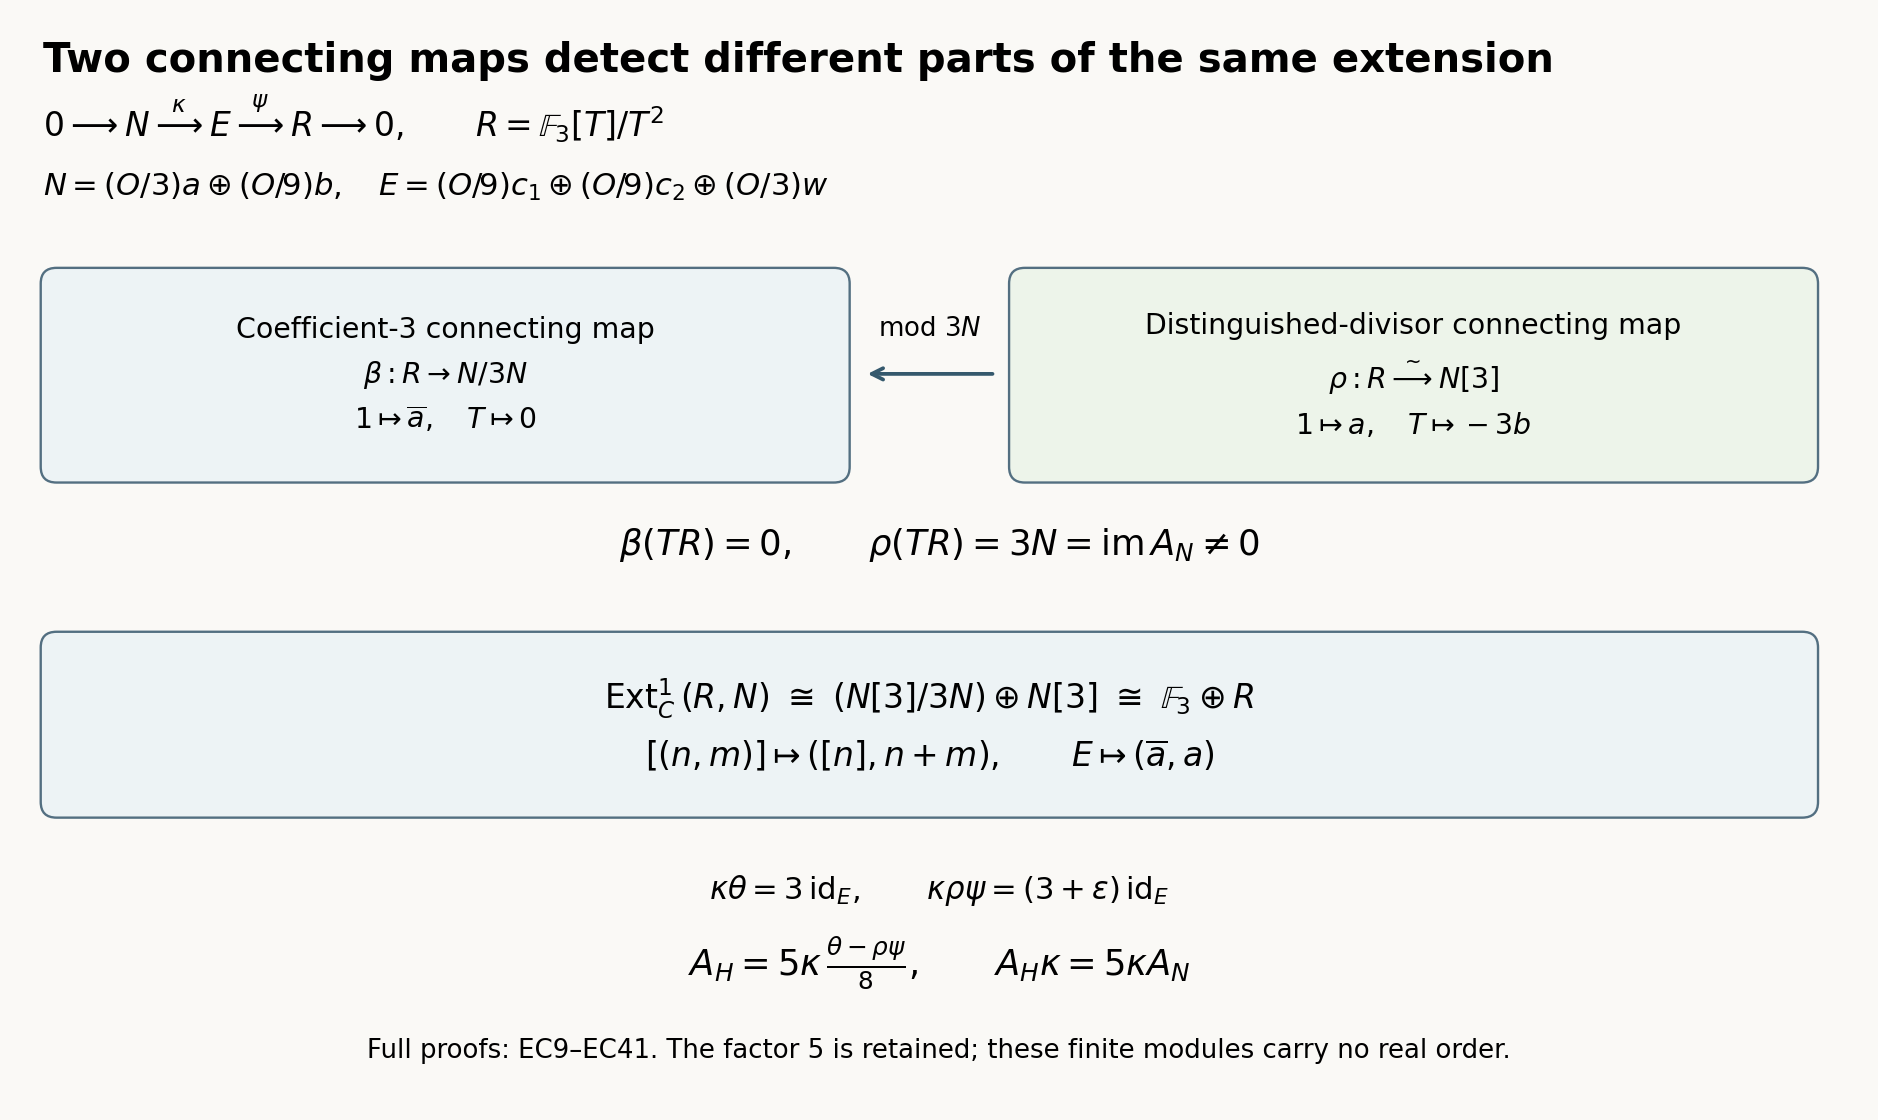
\includegraphics[keepaspectratio,alt={The two connecting maps, their extension coordinates, and their exact divided-residue factorization. Full proofs EC9--EC41.}]{collision_extension_connecting_maps.png}}
\caption{The two connecting maps, their extension coordinates, and their
exact divided-residue factorization. Full proofs EC9--EC41.}
\end{figure}

\clearpage

\section{The distinguished collision prism and its actual module
specializations}\label{the-distinguished-collision-prism-and-its-actual-module-specializations}

Independent derivation, 23 September 2026.

The element \(3+\epsilon\) already occurring in the radical--cotangent
extension defines a bounded prism on the retained four-state integral
collision algebra. This proof constructs that prism, its exact map from
the original unsplit algebra, and the specializations of the original
nilradical and cotangent modules. It retains the given Frobenius
parameter and original residue coefficients.

The source definitions are Bhargav Bhatt and Peter Scholze,
\href{https://arxiv.org/src/1905.08229v4}{\emph{Prisms and Prismatic
Cohomology}, arXiv:1905.08229v4, original author source}, labels
DefPrismCat, FrobLiftTheta, distinguishedDivide, prismcrit, and
PrismMapTaut. The local original-source reading record is given in DP11.
Every application to the programme algebras is proved below.

\subsection{DP1. Original algebras and the retained Frobenius
family}\label{dp1.-original-algebras-and-the-retained-frobenius-family}

Let \(O=\mathbb Z_3\), fix \(c\in O\), and retain \[
B=O[x,T]/(x^2(x+3),T^2-3x(x+2)),\qquad
C=O[\epsilon,T]/(\epsilon^2,T^2-6\epsilon).
\tag{DP1}
\] Successive monic division gives the free \(O\)-bases \[
1,x,x^2,T,xT,x^2T,\qquad 1,\epsilon,T,\epsilon T.
\tag{DP2}
\] The quotient \(q:B\to C\), \(x\mapsto\epsilon,T\mapsto T\), is onto
and has kernel \[
J=(x^2)=Ox^2\oplus Ox^2T.
\tag{DP3}
\]

Put \(n_1=x(x+3)\), \(n_2=T(x+3)\), \(n_3=Tx(x+3)\). The retained
Frobenius maps fix \(O\) and have values \[
\phi_B(x)=0,\qquad\phi_B(T)=3c\,n_3;
\] \[
\phi_C(\epsilon)=0,\qquad\phi_C(T)=9c\,\epsilon T.
\tag{DP4}
\] They are algebra homomorphisms: \(n_3^2=0\) and \((\epsilon T)^2=0\),
so the quadratic relations map to zero, and the other relations map to
zero because \(x,\epsilon\) do. Modulo 3, both maps are Frobenius. On
\(B/3\), \(x^3=T^3=0\); on \(C/3\), \(\epsilon^3=T^3=0\); and constants
have the usual characteristic-three Frobenius.

Both rings are 3-torsionfree, so \[
\delta_A(f)=\frac{\phi_A(f)-f^3}{3}\quad(A=B,C)
\tag{DP5}
\] is a well-defined integral operation. Expansion gives \[
\delta_A(f+g)=\delta_A(f)+\delta_A(g)-fg(f+g),
\] \[
\delta_A(fg)=f^3\delta_A(g)+g^3\delta_A(f)+3\delta_A(f)\delta_A(g),
\] and \(\delta_A(0)=\delta_A(1)=0\), proving the delta-ring identities
directly. In particular \[
\delta_B(x)=x^2,\qquad
\delta_B(T)=c\,n_3-x(x+2)T,
\] \[
\delta_C(\epsilon)=0,\qquad
\delta_C(T)=(3c-2)\epsilon T.
\tag{DP6}
\] The quotient satisfies \(q\phi_B=\phi_Cq\), because
\(q(n_3)=3\epsilon T\). Applying DP5 and using that \(C\) is
3-torsionfree proves \(q\delta_B=\delta_Cq\). The generator formulas DP6
also verify this equality directly.

The parameter is transported exactly: if the target family in DP4 had
parameter \(c'\), compatibility on \(T\) would require
\(9(c-c')\epsilon T=0\). The free basis DP2 then gives \(c=c'\). Every
\(c\in O\) gives the displayed compatible pair; no reduction of that
parameter is being substituted.

\subsection{DP2. The distinguished element and all of its
torsion}\label{dp2.-the-distinguished-element-and-all-of-its-torsion}

Retain the two corresponding elements \[
a_B=3+x,\qquad a_C=3+\epsilon.
\tag{DP7}
\] They satisfy \[
a_C(3-\epsilon)=9.
\tag{DP8}
\] If \(a_C f=0\), multiplication by \(3-\epsilon\) gives \(9f=0\), so
\(f=0\) by DP2. Thus \(a_C\) is a nonzerodivisor.

In \(B\), multiplication of a general coefficient polynomial gives \[
(3+x)(p_0+p_1x+p_2x^2)
=3p_0+(p_0+3p_1)x+p_1x^2.
\] It vanishes exactly when \(p_0=p_1=0\). The same calculation applies
to the \(T\)-coefficient polynomial. Therefore \[
\operatorname{Ann}_B(a_B)=J.
\] For every \(r\ge1\), \[
\operatorname{Ann}_B(a_B^r)=J.
\tag{DP9}
\] Indeed, if \(a_B^r f=0\), applying \(q\) gives \(a_C^r q(f)=0\), so
\(q(f)=0\) and \(f\in J\). Conversely \(a_B J=0\). Hence the quotient
\(q\) kills exactly all \(a_B\)-power torsion, with no additional
elements.

The Frobenius and delta values are \[
\phi_B(a_B)=\phi_C(a_C)=3,
\] \[
\delta_B(a_B)=-8-9x-2x^2,\qquad
\delta_C(a_C)=-8-9\epsilon.
\tag{DP10}
\] For \(B\), expand \((3+x)^3\) and use \(x^3=-3x^2\); for \(C\), use
\(\epsilon^2=0\). Both delta values are units, with exact inverses \[
\delta_B(a_B)^{-1}=-\frac18+\frac9{64}x+\frac{11}{64}x^2,
\] \[
\delta_C(a_C)^{-1}=-\frac18+\frac9{64}\epsilon.
\tag{DP11}
\] Multiplying and reducing by \(x^3=-3x^2,x^4=9x^2\), or by
\(\epsilon^2=0\), proves these formulas. All denominators are powers of
2 and are units in \(O\).

Thus both elements are distinguished, meaning their delta values are
units. The pair \((B,(a_B))\) fails the Cartier-divisor condition, since
the nonzero ideal \(J\) annihilates \(a_B\). The quotient \(C\) removes
precisely this obstruction, by DP9.

\subsection{DP3. Complete verification of the bounded-prism
axioms}\label{dp3.-complete-verification-of-the-bounded-prism-axioms}

A prism at 3 is a delta-ring \(A\) with a Cartier ideal \(I\), derived
\((3,I)\)-complete, and satisfying \(3\in I+\phi(I)A\). It is bounded
when \(A/I\) has bounded \(3\)-power torsion.

Take \(I_C=(a_C)\). It is Cartier by DP8. Since \(\phi_C(a_C)=3\), \[
3\in\phi_C(I_C)C,
\tag{DP12}
\] which proves the required ideal containment.

For completeness, retain the exact ideals \[
(3,a_C)=(3,\epsilon),\qquad
(3,\epsilon)^r=(3^r,3^{r-1}\epsilon)\quad(r\ge1).
\tag{DP13}
\] The second formula follows by expanding a product of \(r\) generators
and using \(\epsilon^2=0\). These powers are cofinal with the powers of
\((3)\). Since \(C\) is finite free over the complete ring \(O\), its
ordinary completion for this ideal is \(C\).

There is also a direct derived-completeness calculation. Use the Koszul
tower \[
K_r=\operatorname{Kos}_C(3^r,\epsilon^r).
\] For \(r\ge2\), one has \(\epsilon^r=0\), and \(3^r\) is regular. Thus
the only cohomology groups of \(K_r\) are \(C/3^rC\) in degrees 0 and
\(-1\). The transition \(K_{r+1}\to K_r\) multiplies the generator for
\(3^{r+1}\) by 3 and the generator for \(\epsilon^{r+1}\) by
\(\epsilon\). On degree-zero cohomology the transition is reduction; on
degree-minus-one cohomology it includes multiplication by \(\epsilon\).
Every two-step transition in the latter tower is therefore zero.

The degree-zero tower is surjective, so its higher inverse limit
vanishes and its inverse limit is \(C\). The degree-minus-one tower is
pro-zero, so both its inverse limit and higher inverse limit vanish. The
inverse-limit cohomology sequence for these bounded complexes
consequently gives \[
R\!\varprojlim_r K_r\simeq C
\] in degree zero. This proves derived \((3,\epsilon)\)-completeness,
hence derived \((3,a_C)\)-completeness, with the actual transition maps
specified.

The \(a_C\)-adic topology itself is also cofinal with the 3-adic
topology: \[
a_C^2=9+6\epsilon\in3C,\qquad9\in a_CC.
\tag{DP14}
\] Indeed \(a_C^{2r}C\subset3^rC\) and \(3^{2r}C\subset a_C^rC\). No
inversion of 3 or of \(a_C\) is involved.

The quotient is exactly \[
D:=C/(a_C)\xrightarrow{\sim}(O/9O)[T]/T^2,
\qquad \epsilon\mapsto-3,\quad T\mapsto T.
\tag{DP15}
\] To verify this, impose \(\epsilon=-3\). The relation \(\epsilon^2=0\)
becomes \(9=0\), and \(T^2-6\epsilon=0\) becomes \(T^2+18=0\), which is
\(T^2=0\) modulo 9. These substitutions define inverse maps. The
quotient is killed by 9, and its element 1 has additive order 9. Hence
its full \(3\)-power torsion has exact exponent 9.

It follows from DP8 and DP12--DP15 that \[
\boxed{(C,(3+\epsilon))\text{ is a bounded, oriented prism}.}
\tag{DP16}
\] This holds for every retained parameter \(c\in O\).

\subsection{DP4. The exact universal quotient and its prism
form}\label{dp4.-the-exact-universal-quotient-and-its-prism-form}

The map \(q\) is universal among delta-maps from \(B\) for which the
image of \(a_B\) is regular. Precisely, let \(f:B\to A\) be a delta-ring
map and assume multiplication by \(f(a_B)\) is injective on \(A\). For
\(j\in J\), \[
f(a_B)f(j)=f(a_Bj)=0,
\] so \(f(j)=0\). There is therefore a unique ring map
\(\overline f:C=B/J\to A\) with \(\overline f q=f\). It is a delta-map:
for \(b\in B\), \[
\overline f(\delta_C(qb))
=\overline f(q\delta_Bb)
=f(\delta_Bb)
=\delta_A(fb).
\] Surjectivity of \(q\) proves the required compatibility for every
element of \(C\). This establishes the universal property with its exact
domain of targets.

For prism targets there is a stronger formulation. A distinguished
element \(d\) belonging to the Cartier ideal \(I\) of a prism \((A,I)\)
generates \(I\), and is therefore regular. Here is the argument with its
hypotheses retained. The original prism criterion supplies a faithfully
flat delta-localization \(A\to A'\) on which \(IA'=(e)\), with \(e,3\)
in the Jacobson radical. Write \(d=eu\) there. The delta product
identity gives \[
\delta(d)=e^3\delta(u)+u^3\delta(e)+3\delta(e)\delta(u).
\] The left side is a unit, and the first and third terms on the right
lie in the Jacobson radical. Consequently \(u^3\delta(e)\) is a unit,
and hence \(u\) is a unit. Thus \(IA'=(d)\). Faithful flatness descends
the ideal equality \(I=(d)\); regularity follows after the same cover,
where \(d\) is a unit times the regular Cartier generator \(e\).

Apply this to a delta-map \(f:B\to A\) with \((A,I)\) a prism and
\(f(a_B)\in I\). The element \(f(a_B)\) is distinguished because the
unit in DP10 maps to \(\delta_A(f(a_B))\). It therefore generates \(I\)
and is regular. The factorization just proved gives a unique prism
morphism \[
(C,(a_C))\longrightarrow(A,I).
\tag{DP17}
\] Thus DP16 is the initial prism equipped with such a delta-map from
the original \(B\) carrying \(a_B\) into its prism ideal. This is a
property of the specified original element and specified Frobenius
family. It does not assert a prism structure with ideal \((a_B)\) on
\(B\).

\subsection{DP5. The actual map to the crystalline
prism}\label{dp5.-the-actual-map-to-the-crystalline-prism}

The same delta-ring \(C\) also supports the bounded crystalline prism
\((C,(3))\): multiplication by 3 is injective, \(C\) is derived
3-complete by its free \(O\)-basis, \(3\in(3)\), and \(C/3\) has its
\(3\)-torsion killed by 3.

The Frobenius \(\phi_C\) is itself a delta-map. Indeed, in the
3-torsionfree ring \(C\), applying \(\phi_C\) to DP5 and using that it
fixes 3 gives \[
3\phi_C(\delta_C f)=\phi_C^2(f)-\phi_C(f)^3
=3\delta_C(\phi_C f).
\] Cancelling 3 proves the assertion. Since \(\phi_C(a_C)=3\), it
defines a prism morphism \[
\phi_C:(C,(3+\epsilon))\longrightarrow(C,(3)).
\tag{DP18}
\] The extended image of the source ideal is exactly \((3)\).

The identity ring map is a prism morphism in neither direction. One has
\(a_C\notin3C\), since its \(\epsilon\)-coefficient is 1 in the free
basis. Also \(3\notin a_CC\), since 3 has nonzero image in the
characteristic-nine quotient DP15.

On prism quotients, DP18 induces the exact map \[
D=(O/9O)[T]/T^2\longrightarrow
C/3=\mathbb F_3[\epsilon,T]/(\epsilon^2,T^2),
\qquad T\mapsto0,\quad \overline z\mapsto z\bmod3.
\tag{DP19}
\] Its image is the constants \(\mathbb F_3\), and its kernel is
\((3,T)\subset D\). These formulas follow immediately from DP4,
including its factor \(9c\).

\subsection{DP6. The nilradical quotient is this prism
specialization}\label{dp6.-the-nilradical-quotient-is-this-prism-specialization}

Retain \[
N_B=On_1\oplus On_2\oplus On_3,\qquad
N_C=O\epsilon\oplus OT\oplus O\epsilon T.
\tag{DP20}
\] These are the original nilradicals. For \(C\), the stated ideal is
nilpotent and its quotient is the reduced ring \(O\). For \(B\),
evaluation at \((0,0),(-3,3),(-3,-3)\) has precisely this kernel: a
coefficient expression \(p(x)+Tq_0(x)\) is killed by all three maps
exactly when \(p(0)=p(-3)=q_0(-3)=0\), giving the displayed three
generators. Their products satisfy \[
n_1^2=n_1n_3=n_2n_3=n_3^2=0,\quad
n_1n_2=3n_3,\quad n_2^2=18n_1,
\] so that kernel is nilpotent. Every nilpotent must vanish in the
reduced evaluation target, proving equality with the nilradical.

The actions are \[
xn_1=xn_3=0,\quad xn_2=n_3,\qquad
Tn_1=n_3,\quad Tn_2=6n_1,\quad Tn_3=0.
\tag{DP21}
\] In particular \(JN_B=0\), so \(N_B\) is a \(C\)-module through \(q\).
The map \[
i:N_B\xrightarrow{\sim}N_C,\qquad
n_1\mapsto\epsilon,\quad n_2\mapsto T,\quad n_3\mapsto\epsilon T
\tag{DP22}
\] is \(C\)-linear: every generator action in DP21 agrees with
multiplication by \(\epsilon,T\) on its images. Its basis map is
bijective.

The actual quotient-induced map \(q_N\) is \[
q_N(n_1)=3\epsilon,\quad
q_N(n_2)=3T+\epsilon T,\quad
q_N(n_3)=3\epsilon T.
\] Thus \[
\boxed{q_N=m_{a_C}\circ i.}
\tag{DP23}
\] Multiplication by \(a_C\) is injective on \(N_C\), since it is
injective on \(C\). Therefore \[
Q_N=\operatorname{coker}q_N
=N_C/a_CN_C
\simeq N_C\otimes_C^{\mathbf L}D
\tag{DP24}
\] with the derived tensor concentrated in degree zero. To prove the
derived assertion, use the free resolution
\(0\to C\xrightarrow{a_C}C\to D\to0\). Tensoring gives the two-term map
\(a_C:N_C\to N_C\), whose kernel is zero; its cokernel is exactly DP24.

There is also an injection \(N_C/a_CN_C\to C/a_CC\). If
\(a_C f\in N_C\), its constant coefficient is \(3f_0\). That coefficient
vanishes only when \(f_0=0\), so \(f\in N_C\). Hence
\(N_C\cap a_CC=a_CN_C\), proving injection. Under DP15 its image is
precisely \[
\boxed{Q_N\xrightarrow{\sim}(3,T)\subset D,\qquad
[\epsilon]\mapsto-3,\quad[T]\mapsto T.}
\tag{DP25}
\] The ideal \((3,T)\) is nilpotent, with \[
(3,T)^2=(3T),\qquad(3,T)^3=0.
\] Its quotient in \(D\) is \(\mathbb F_3\), which is reduced, so it is
exactly \(\operatorname{Nil}(D)\). Thus the same \(Q_N\) is the original
module specialization, the nilradical of the prism quotient, and the
kernel of DP19.

In original generators \(a=[\epsilon]\), \(b=[T]\), its module
presentation remains \[
Q_N=(O/3O)a\oplus(O/9O)b,\qquad[\epsilon T]=-3b.
\tag{DP26}
\] The sign agrees with the embedding \(\epsilon\mapsto-3\) in DP25.

\subsection{DP7. Both cotangent quotients and their exact
comparison}\label{dp7.-both-cotangent-quotients-and-their-exact-comparison}

Retain the original relative cotangent kernels \[
H_B=H^{-1}(L_{B/O}),\qquad H_C=H^{-1}(L_{C/O}).
\] Their free bases are \[
u_1=(n_1,0),\quad u_2=(n_3,0),\quad u_3=(n_2,n_3);
\] \[
v_1=(\epsilon,0),\quad v_2=(\epsilon T,0),\quad
v_3=(3T,\epsilon T).
\tag{DP27}
\] These are kernels of the respective Jacobian matrices \[
\begin{pmatrix}3x(x+2)&-6(x+1)\\0&2T\end{pmatrix},
\qquad
\begin{pmatrix}2\epsilon&-6\\0&2T\end{pmatrix}.
\] For completeness, let \(A_0=O[x]/(x^2(x+3))\). Multiplication by
\(x\) sends \(p_0+p_1x+p_2x^2\) to \(p_0x+(p_1-3p_2)x^2\), so its kernel
is \(On_1\). Also \(x+2\) is a unit, with inverse \(1/2-x/4-x^2/4\).
Writing \(B=A_0\oplus TA_0\), the equation \(T(p+Tq_0)=0\) forces
\(p=0\) and \(3x(x+2)q_0=0\). Freeness permits cancellation of 3, and
the unit inverse gives \(q_0\in On_1\). Thus
\(\operatorname{Ann}_B(T)=On_3\) and
\(\operatorname{Ann}_B(T^2)=On_1\oplus On_3\). In the first Jacobian
kernel, the lower equation gives \(b=zn_3\), and the upper equation
gives \(T^2a=6zn_3\), since \((x+1)n_3=n_3\). Since \(T^2n_2=6n_3\),
this means \(a-zn_2\in On_1\oplus On_3\), exactly the three displayed
cycles. For the second kernel, coefficient comparison in the free basis
of \(C\) gives \(\operatorname{Ann}_C(T)=O\epsilon T\); the equation
\(\epsilon a=3b\) then gives its stated basis. These are the original
presentations, with no coordinate change.

The maps previously proved in NC18--NC19 are \[
\kappa_B(n_1)=u_1,\quad\kappa_B(n_2)=u_3,\quad
\kappa_B(n_3)=u_2;
\] \[
\kappa_C(\epsilon)=3v_1,\quad
\kappa_C(T)=v_3-2v_2,\quad
\kappa_C(\epsilon T)=3v_2.
\tag{DP28}
\] The first is a \(C\)-linear isomorphism and the second a \(C\)-linear
injection. Their linearity follows from the generator actions \[
\epsilon v_1=\epsilon v_2=0,\quad\epsilon v_3=3v_2,\qquad
Tv_1=v_2,\quad Tv_2=0,\quad Tv_3=18v_1
\] and DP21; injectivity follows from their independent displayed
coefficients. Direct substitution gives \[
q_H(u_1)=9v_1,\quad q_H(u_2)=9v_2,\quad
q_H(u_3)=3v_3-3v_2,
\] and hence the exact factorization \[
\boxed{q_H=\kappa_C\,m_{a_C}\,i\,\kappa_B^{-1}.}
\tag{DP29}
\] Consequently the actual cotangent cokernel is \[
Q_H=H_C/(a_C\kappa_C(N_C)).
\tag{DP30}
\] This is connected to the prism specialization of the entire \(H_C\)
by the surjection \[
Q_H\longrightarrow H_C/a_CH_C.
\] Multiplication by \(a_C\) is injective on the \(O\)-free module
\(H_C\): if \(a_C h=0\), then \(9h=(3-\epsilon)a_C h=0\). Its induced
map therefore identifies \[
a_CH_C/(a_C\kappa_C(N_C))
\simeq H_C/\kappa_C(N_C).
\] The latter is \(R=\mathbb F_3[T]/T^2\), via
\([v_1]\mapsto1,[v_2]\mapsto T,[v_3]\mapsto2T\). This yields the exact
sequence \[
0\longrightarrow R\xrightarrow{\,a_C\,}Q_H
\longrightarrow H_C/a_CH_C\longrightarrow0.
\tag{DP31}
\] The first arrow means: lift a class from \(H_C/\kappa_C(N_C)\),
multiply its lift by \(a_C\), and take its class in DP30. It is well
defined and injective by the preceding cancellation proof.

The second quotient is explicitly \[
H_C/a_CH_C\simeq\mathbb F_3\{[v_1],[v_2],[v_3]\}
\simeq R\oplus\mathbb F_3
\tag{DP32}
\] as \(C\)-modules. Indeed \(a_Cv_1=3v_1\), \(a_Cv_2=3v_2\), and
\(a_Cv_3=3v_3+3v_2\), so the quotient has exactly the three relations
\(3v_j=0\). There \(\epsilon\) acts as zero, \(T[v_1]=[v_2]\), and
\(T[v_2]=T[v_3]=0\), giving the displayed module decomposition. Its
derived specialization is again concentrated in degree zero because
\(a_C\) is injective on \(H_C\).

Thus DP30 and DP32 have both their actual presentations and their
connecting maps. In particular \(Q_H\), of order \(3^5\), is not
replaced by the order-\(3^3\) specialization DP32.

\subsection{DP8. The prism element in the original
extension}\label{dp8.-the-prism-element-in-the-original-extension}

Use the original notation \[
Q_N=(O/3)a\oplus(O/9)b,\qquad
Q_H=(O/9)c_1\oplus(O/9)c_2\oplus(O/3)w,
\] where \(c_1=[v_1]\), \(c_2=[v_2]\), \(w=[v_3-v_2]\). The original
extension maps are \[
\kappa(a)=3c_1,\quad\kappa(b)=w-c_2,\qquad
\psi(c_1)=1,\quad\psi(c_2)=\psi(w)=T.
\tag{DP33}
\] The connecting map associated with the annihilator element \(a_C\) is
\[
\rho:R\to Q_N[3],\qquad
\rho(1)=a,\quad\rho(T)=-3b.
\] It is an isomorphism by the original \(T\)-action \(Ta=-3b\). Direct
multiplication gives \[
\boxed{a_C\,\mathrm{id}_{Q_H}=\kappa\rho\psi.}
\tag{DP34}
\] On \(c_1,c_2,w\), the two sides are respectively \(3c_1,3c_2,3c_2\),
since \(3w=0\) and \(\epsilon w=3c_2\). Therefore \[
a_C^2Q_H=0,\quad
a_CQ_H=\kappa(Q_N[3]),\quad
\ker(a_C:Q_H\to Q_H)=\kappa(Q_N).
\tag{DP35}
\] The image has order 9 and identifies with the kernel in DP31. The
kernel assertion follows from DP34 and injectivity of \(\kappa,\rho\).

Retain also the coefficient-3 map \[
\theta:Q_H\to Q_N,\qquad
\kappa\theta=3\,\mathrm{id}_{Q_H},
\] whose values are \(\theta(c_1)=a,\theta(c_2)=-3b,\theta(w)=0\). Then
the original divided cotangent operator has the exact expression \[
L=-\frac{5\epsilon}{8}
=\frac{5(3-a_C)}8
=\frac58\,\kappa(\theta-\rho\psi).
\tag{DP36}
\] This is an equality of actual integral endomorphisms on \(Q_H\), not
division of a torsion map by 3. It relates the coefficient-3 connecting
map and the prism-element connecting map with the original coefficient 5
retained.

\subsection{DP9. The residue descends to a nonzero derivation on the
prism
quotient}\label{dp9.-the-residue-descends-to-a-nonzero-derivation-on-the-prism-quotient}

The original integral residues are \[
D_B(x)=0,\quad D_B(T)=-n_3/8,\qquad
D_C(\epsilon)=0,\quad D_C(T)=-3\epsilon T/8.
\tag{DP37}
\] They preserve the defining relations by \(T^2n_1=0\) and
\(\epsilon^2=0\), respectively. They commute with \(q\). For the
Frobenius family DP4, \[
D_B\phi_B=\phi_BD_B=0,\qquad
D_C\phi_C=\phi_CD_C=0.
\] Indeed the images of the residues are the coefficient lines \(On_3\)
and \(O\epsilon T\), respectively; Frobenius kills these lines, and the
residue kills every Frobenius image. This is compatibility with the
stated Frobenius, not an assertion of commutation with the nonlinear
delta operation.

On the whole algebra \(C\), the divided operator is an integral
derivation: \[
\partial=\frac{D_C}{3},\qquad
\partial(\epsilon)=0,\quad\partial(T)=-\epsilon T/8.
\tag{DP38}
\] Its action on \(T^2-6\epsilon\) is
\(-\epsilon T^2/4=-3\epsilon^2/2=0\), and its action on \(\epsilon^2\)
is zero, proving that it descends from the polynomial algebra. It fixes
\(a_C\), so it induces a derivation on DP15. Its exact formula there is
\[
\overline\partial:(O/9)[T]/T^2\longrightarrow(O/9)[T]/T^2,
\qquad
\overline\partial(z_0+z_1T)=\frac38z_1T.
\tag{DP39}
\] It kills constants and is nonzero, since \(3T\ne0\). Its square and
its triple are zero. The unscaled \(D_C=3\partial\) consequently induces
the zero derivation on the prism quotient.

Under the actual nilradical identification DP25, its restriction is
exactly \[
A_N(a)=0,\qquad A_N(b)=\frac38b.
\tag{DP40}
\] In particular its image is the ideal
\((3T)=\operatorname{Nil}(D)^2\), of order 3. It is not multiplication
by \(3/8\) on the whole ring \(D\), since its value at 1 is zero;
multiplication by \(3/8\) describes only its restriction to the
nilradical, where \(3\cdot3=0\).

The asymmetry with the source \(B\) is exact. Dividing \(D_B(T)\) by 3
would give \[
-\frac{x^2T}{24}-\frac{xT}{8},
\] whose \(x^2T\)-coefficient does not belong to \(O\). Thus \(D_B/3\)
is not an integral algebra derivation on \(B\), although its original
restriction to \(N_B\) is divisible by 3, as proved in NC36--NC43. The
map to \(C\), and then the prism specialization, are the specified
morphisms relating these facts.

\subsection{DP10. The exact ordinary
spectra}\label{dp10.-the-exact-ordinary-spectra}

The nilradical of \(C\) is \(N_C=(\epsilon,T)\), as proved in DP20, and
\(C/N_C=O\). Every prime ideal contains the nilradical. Since
\(O=\mathbb Z_3\) has exactly the prime ideals \((0)\) and \((3)\), the
complete ordinary spectrum is \[
\operatorname{Spec}(C)=\{\mathfrak n_C,\mathfrak m_C\},\qquad
\mathfrak n_C=(\epsilon,T),\quad
\mathfrak m_C=(3,\epsilon,T).
\tag{DP41}
\] Here \(\mathfrak n_C\subset\mathfrak m_C\); the first point is
generic and the second closed. The quotient rings by these ideals are
respectively \(O\) and \(\mathbb F_3\), so each displayed ideal is prime
and the list is exhaustive.

For the actual prism quotient, DP25 proves \[
\operatorname{Nil}(D)=(3,T)=:\mathfrak m_D,\qquad
D/\mathfrak m_D=\mathbb F_3.
\tag{DP42}
\] Thus \(\operatorname{Spec}(D)\) has the single prime
\(\mathfrak m_D\). The quotient map \(C\to D\) pulls it back to
\(\mathfrak m_C\): the three elements \(3,\epsilon,T\) map into
\((3,T)\), while the residual scalar map is reduction modulo 3.
Therefore the ordinary closed immersion has image \[
\operatorname{Spec}(D)\longrightarrow\operatorname{Spec}(C),\qquad
\mathfrak m_D\longmapsto\mathfrak m_C,
\quad\operatorname{im}=V(a_C)=\{\mathfrak m_C\}.
\tag{DP43}
\] Indeed the image of \(a_C\) in \(C/\mathfrak n_C=O\) is the nonzero
scalar 3, so \(\mathfrak n_C\) does not contain \(a_C\), whereas
\(\mathfrak m_C\) does. This is specialization at the prime 3 with the
complete characteristic-nine nilpotent structure of \(D\) retained. In
particular \(D[1/3]=0\), but \(3\) and \(T\) are both nonzero in \(D\).

\subsection{DP11. Exact source-reading and use
record}\label{dp11.-exact-source-reading-and-use-record}

Canonical source ID: PUBUNIT-3372AF0EC9F522F58C6F6CEE.

Authors: Bhargav Bhatt and Peter Scholze. Title: \emph{Prisms and
Prismatic Cohomology}. Version: arXiv:1905.08229v4, original author
source archive retained locally. The existing machine-readable route
sources/prismatic/prisms\_index\_routes.json was consulted before
reading. The actual original source read is
\texttt{sources/\allowbreak{}prismatic/\allowbreak{}1905.\allowbreak{}08229v4/\allowbreak{}prisms.\allowbreak{}tex}, SHA256
\texttt{f155d205\allowbreak{}1758e280\allowbreak{}5efad851\allowbreak{}3690a91d\allowbreak{}7b18c194\allowbreak{}61514abd\allowbreak{}fd3d32f1\allowbreak{}676cf38b}.

Actual bounded reading for this derivation: source lines 134--180 for
introductory prism and boundedness definitions; 484--558 for delta-ring
identities, Frobenius lifts, and quotient compatibility; 689--742 for
distinguished-element products and division; 936--1084 for Koszul
conventions, the exact prism definition DefPrismCat, prismcrit, rigidity
PrismMapTaut, and the start of the bounded-prism properties. These
original LaTeX portions were read directly. The rest of that paper is
not claimed as newly read here.

The received mathematical uses are precise: DP1 applies the delta-ring
definition directly to the retained Frobenius family; DP3 checks every
prism and boundedness axiom; DP4 applies the distinguished-division
argument and the source's faithfully flat delta-localization
construction; DP5 uses the definition of a prism morphism. All
specialised identities, torsion kernels, coefficient signs, completeness
calculations, and module specializations are proved in this file.

Incoming programme proofs are
\href{https://github.com/KokunoYumeto/zeta-function-research-reader/blob/5a89872598df0902b7c1393cf8e4692ca3010a95/workbenches/splitzero-tandem/branches/tau-zero-prime-positivity/research_calculations/INTEGRAL_EIGHT_STATE_COLLISION_DERIVATION.md}{Integral
eight-state collision proof}, the original integral algebra and
Frobenius calculations;
\href{https://github.com/KokunoYumeto/zeta-function-research-reader/blob/5a89872598df0902b7c1393cf8e4692ca3010a95/workbenches/splitzero-tandem/branches/tau-zero-prime-positivity/research_calculations/NILRADICAL_COTANGENT_DIVIDED_RESIDUE_DERIVATION.md}{Nilradical
and cotangent divided-residue proof}, NC1--NC43; and
\href{NILRADICAL_COTANGENT_EXTENSION_CLASS_DERIVATION.md}{Integral
extension-class proof}, EC1--EC48. This is a construction of a specific
bounded prism and its actual module maps. It does not identify ordinary
de Rham or cotangent cohomology with an uncomputed prismatic cohomology
group.

\clearpage

\section{Supported-zero spectra of the collision
prism}\label{supported-zero-spectra-of-the-collision-prism}

23 September 2026. This proof computes the prime-spectrum maps of the
actual coefficient and divisor quotients. Supported zero and the
unsupported element remain distinct throughout.

The original semiring conventions and the integer spectrum are proved in
\href{https://github.com/KokunoYumeto/zeta-function-research-reader/blob/5a89872598df0902b7c1393cf8e4692ca3010a95/workbenches/splitzero-tandem/branches/tau-zero-prime-positivity/supporting_proofs/TAU_PRIME_SPECTRUM_DERIVATION.md}{TPS1--TPS8}.
The original collision algebras and nilradical quotient are
\href{https://github.com/KokunoYumeto/zeta-function-research-reader/blob/5a89872598df0902b7c1393cf8e4692ca3010a95/workbenches/splitzero-tandem/branches/tau-zero-prime-positivity/research_calculations/NILRADICAL_COTANGENT_DIVIDED_RESIDUE_DERIVATION.md}{NC1--NC13}.
Their spectra and all maps used here are proved below.

\subsection{SG1. The original supported semiring and all its prime
ideals}\label{sg1.-the-original-supported-semiring-and-all-its-prime-ideals}

For a nonzero commutative unital ring \(A\), set \[
G(A)=\{\tau\}\sqcup A^\bullet,\qquad e_A=0_A^\bullet.
\tag{SG1}
\] Here the bullet is a label, so \(e_A\ne\tau\). Define \[
a^\bullet+b^\bullet=(a+b)^\bullet,\quad
a^\bullet b^\bullet=(ab)^\bullet,\quad
z+\tau=z,\quad z\tau=\tau.
\tag{SG2}
\] These operations form a commutative semiring with additive identity
\(\tau\) and multiplicative identity \(1_A^\bullet\). Associativity and
distributivity for entirely supported arguments are the corresponding
ring identities. If an argument is \(\tau\), its additive-identity and
multiplicatively absorbing rules give the identities directly. These
cases exhaust all arguments.

An ideal contains \(\tau\), is closed under addition, and under
multiplication by every semiring element. Its intersection with
\(A^\bullet\) is either empty or \(I^\bullet\) for a ring ideal
\(I\subset A\). Indeed multiplication by \(e_A\) produces \(e_A\) from
any supported member; multiplication by \((-1_A)^\bullet\) supplies
supported additive inverses. The other ring-ideal properties are the
given closure properties. Conversely these properties prove that every
set \[
P_\tau(A)=\{\tau\},\qquad
P_I(A)=\{\tau\}\cup I^\bullet
\tag{SG3}
\] is a semiring ideal. This classifies all ideals, including the whole
semiring when \(I=A\).

A proper ideal is prime if membership of a product forces membership of
a factor. A product of supported elements is supported, so \(P_\tau(A)\)
is prime for every \(A\). For \(P_I(A)\), products of supported elements
give exactly the ring prime-ideal test for \(I\), and products involving
\(\tau\) already satisfy the test. Thus \[
\operatorname{Spec}G(A)=\{P_\tau(A)\}\sqcup
\{P_{\mathfrak p}(A):\mathfrak p\in\operatorname{Spec}A\}.
\tag{SG4}
\] Every arithmetic point \(P_{\mathfrak p}(A)\) contains \(e_A\). The
point \(P_\tau(A)\) does not, and is contained strictly in every
arithmetic point. The topology has basic opens \(D(z)=\{P:z\notin P\}\).
For a supported element, \[
D(a^\bullet)=\{P_\tau(A)\}\cup
\{P_{\mathfrak p}(A):a\notin\mathfrak p\},\quad
D(e_A)=\{P_\tau(A)\}.
\tag{SG5}
\] These formulas prove that the arithmetic points form the closed
subspace \(V(e_A)\), homeomorphic to \(\operatorname{Spec}A\).

For a unital ring map \(f:A\to A'\), the map \(G(f)\) sends \(\tau\) to
\(\tau\) and \(a^\bullet\) to \(f(a)^\bullet\). It preserves both
operations and both identities. Its spectrum map is precisely \[
G(f)^*P_\tau(A')=P_\tau(A),\qquad
G(f)^*P_{\mathfrak p'}(A')=P_{f^{-1}\mathfrak p'}(A).
\tag{SG6}
\] Taking preimages of the basic opens proves continuity. No supported
element is mapped to \(\tau\).

\subsection{SG2. The coefficient algebra and its distinguished
divisor}\label{sg2.-the-coefficient-algebra-and-its-distinguished-divisor}

Put \(O=\mathbb Z_3\), the ring of 3-adic integers, and retain \[
B=O[x,T]/(x^2(x+3),T^2-3x(x+2)),\qquad
C=O[\epsilon,T]/(\epsilon^2,T^2-6\epsilon).
\tag{SG7}
\] The map \(q:B\twoheadrightarrow C\) sends \(x\) to \(\epsilon\) and
\(T\) to \(T\); substituting gives both relations of \(B\). Its images
generate \(C\), so it is onto. Successive division by the monic
equations gives the free \(O\)-basis \(1,\epsilon,T,\epsilon T\) of
\(C\).

Set \[
\mathfrak n=(\epsilon,T)\subset C,\qquad
\mathfrak m=(3,\epsilon,T)\subset C,\qquad a_C=3+\epsilon.
\tag{SG8}
\] The equalities \(\epsilon^2=0\) and \(T^2=6\epsilon\) give \[
\mathfrak n^2=(6\epsilon,\epsilon T),\quad
\mathfrak n^3=(6\epsilon T),\quad \mathfrak n^4=0.
\tag{SG9}
\] For instance multiplying the two displayed generators of
\(\mathfrak n^2\) by \(\epsilon,T\) gives exactly the ideal generated by
\(6\epsilon T\); one further multiplication gives zero. The quotient
\(C/\mathfrak n=O\) is reduced. Therefore \(\mathfrak n\) is exactly the
nilradical. Every prime contains every nilpotent (apply primeness
repeatedly to a vanishing power); primes of \(C\) thus correspond
exactly to primes of \(O\).

The primes of \(O\) are \((0)\) and \((3)\). To see completeness, a
nonzero element has the form \(3^k u\), with \(u\) a unit. A nonzero
proper prime containing it must contain 3, and the ideal \((3)\) is
maximal because its quotient is \(\mathbb F_3\). Thus \[
\operatorname{Spec}C=\{\mathfrak n\subsetneq\mathfrak m\}.
\tag{SG10}
\]

Let \(D=C/(a_C)\). In this quotient \(\epsilon=-3\), so \(\epsilon^2=0\)
imposes 9 and \(T^2=6\epsilon\) imposes \(T^2=-18=0\). Conversely these
equations satisfy all the original relations and \(3+\epsilon=0\). The
two substitution maps are inverse, proving \[
D\xrightarrow{\sim}(O/9O)[T]/T^2,\qquad
\epsilon\mapsto-3,\quad T\mapsto T.
\tag{SG11}
\] The ideal \(\mathfrak d=(3,T)\subset D\) satisfies \[
\mathfrak d^2=(3T),\qquad \mathfrak d^3=0,\qquad
D/\mathfrak d=\mathbb F_3.
\tag{SG12}
\] Here \(3T\ne0\), because \(1,T\) is a free \(O/9O\)-basis. These
facts prove that \(\mathfrak d\) is the nilradical and the unique prime
of \(D\). The quotient map \(\pi:C\to D\) pulls it back to
\(\mathfrak m\), since its composite to \(\mathbb F_3\) kills exactly
\((3,\epsilon,T)\).

\subsection{SG3. Every supported point and its exact
pullback}\label{sg3.-every-supported-point-and-its-exact-pullback}

Applying SG4 and SG6 gives the complete chains \[
\operatorname{Spec}G(C):\quad
P_\tau(C)\subsetneq P_{\mathfrak n}(C)\subsetneq P_{\mathfrak m}(C),
\] \[
\operatorname{Spec}G(D):\quad
P_\tau(D)\subsetneq P_{\mathfrak d}(D).
\tag{SG13}
\] The spectrum map of the actual divisor quotient is \[
G(\pi)^*:P_\tau(D)\mapsto P_\tau(C),\qquad
P_{\mathfrak d}(D)\mapsto P_{\mathfrak m}(C).
\tag{SG14}
\] Its image is the two-point subspace
\(\{P_\tau(C),P_{\mathfrak m}(C)\}\). It is a homeomorphism onto this
subspace: its opens are the empty set, the unsupported singleton, and
both points, as follows immediately from SG5 in both spaces. It is not a
closed subset of \(\operatorname{Spec}G(C)\), since it contains the
dense point \(P_\tau(C)\) but omits \(P_{\mathfrak n}(C)\). The ring
closed immersion \(\operatorname{Spec}D\to\operatorname{Spec}C\)
therefore has this explicitly different supported extension. Its inverse
images and topology, rather than an assumed closed-immersion rule for a
semiring congruence quotient, specify the map.

The coefficient inclusion \(O\to C\) pulls \(\mathfrak n\) back to
\((0)\) and \(\mathfrak m\) back to \((3)\). Hence its supported
spectrum map is \[
P_\tau(C)\mapsto P_\tau(O),\quad
P_{\mathfrak n}(C)\mapsto P_{(0)}(O),\quad
P_{\mathfrak m}(C)\mapsto P_{(3)}(O).
\tag{SG15}
\] This is a homeomorphism of the three-point chains, by their basic
opens. The composite \(G(O)\to G(D)\) thus sends its arithmetic point
back to the prime over 3. The pullbacks to the original algebra \(B\)
are also explicit: \[
q^{-1}\mathfrak n=(x,T),\qquad
q^{-1}\mathfrak m=(3,x,T),
\tag{SG16}
\] because the two composite quotients are respectively \(O\) and
\(\mathbb F_3\). Equations SG6 and SG16 give the corresponding supported
prime ideals of \(G(B)\), without claiming a classification of every
other point of \(\operatorname{Spec}G(B)\).

The ideal generated by \(e_C\) is exactly \(\{\tau,e_C\}\): multiplying
a supported element by \(e_C\) yields \(e_C\), and addition does not
produce another element. It is not prime, since
\((\epsilon^\bullet)^2=e_C\) while \(\epsilon^\bullet\) is outside that
ideal. Its radical, defined by powers entering the ideal, is exactly \[
\sqrt{(e_C)}=P_{\mathfrak n}(C).
\tag{SG17}
\] For a supported element, entering \((e_C)\) by a power is exactly
nilpotence in \(C\). This proves SG17 and also gives
\(\sqrt{(e_D)}=P_{\mathfrak d}(D)\). Over the original domain \(O\), the
same calculation gives \((e_O)=P_{(0)}(O)\), which is itself prime. SG15
is therefore the exact map from the collision's nilpotent prime to the
original supported-zero prime; these points are not discarded or
identified with \(P_\tau\).

\subsection{SG4. The infinitesimal quotient as an actual
ideal}\label{sg4.-the-infinitesimal-quotient-as-an-actual-ideal}

Multiplication by \(a_C\) is injective on \(C\), because \[
(3-\epsilon)a_C=9
\tag{SG18}
\] and \(C\) is free over the domain \(O\). Its restriction to
\(\mathfrak n\) is injective as well. Moreover \[
a_C C\cap\mathfrak n=a_C\mathfrak n.
\tag{SG19}
\] Indeed, writing \(f=f_0+f_1\epsilon+f_2T+f_3\epsilon T\), the
constant coefficient of \(a_C f\) is \(3f_0\). If this belongs to
\(\mathfrak n\), then \(f_0=0\), hence \(f\in\mathfrak n\). The other
inclusion is immediate. Consequently the natural quotient map is an
injection \[
\mathfrak n/a_C\mathfrak n\hookrightarrow D
\] with image generated by \(-3,T,-3T\), namely \(\mathfrak d\). Thus \[
\mathfrak n/a_C\mathfrak n\xrightarrow{\sim}\mathfrak d,
\quad [\epsilon]\mapsto-3,\quad[T]\mapsto T,\quad
[\epsilon T]\mapsto-3T.
\tag{SG20}
\] The free resolution \(0\to C\xrightarrow{a_C}C\to D\to0\) shows that
\(\operatorname{Tor}_1^C(\mathfrak n,D)\) is the kernel of
multiplication by \(a_C\) on \(\mathfrak n\), hence zero. All higher Tor
groups vanish because this resolution has length one. This proves that
the same ordinary quotient computes the derived specialization; no
discarded higher group is being assumed to vanish.

For the retained Frobenius family, define \(\Phi_C\) on \(O\) to be the
identity, on \(\epsilon\) to be zero, and on \(T\) by \(9c\epsilon T\),
with \(c\in O\). The images satisfy both relations. Modulo 3, the
original generators have cubes zero, so \(\Phi_C\) lifts the
characteristic-three Frobenius. Since \(\Phi_C(a_C)=3\), it induces the
unital ring map \[
\overline\Phi:D\longrightarrow C/3C,\qquad
f_0+f_1T\longmapsto\overline f_0.
\tag{SG21}
\] The target is \(\mathbb F_3[\epsilon,T]/(\epsilon^2,T^2)\). The
displayed formula proves \(\ker\overline\Phi=\mathfrak d\) and
\(\operatorname{im}\overline\Phi=\mathbb F_3\). Its additive cokernel is
the vector space with basis \(\epsilon,T,\epsilon T\). Both quotient
rings have exactly the primes specified by their nilradicals, so its
supported spectrum map preserves the unsupported point and the sole
arithmetic point. The killed ideal is exactly the retained infinitesimal
ideal SG20, and is recorded as a kernel rather than erased from the
calculation.

Finally the \(O\)-linear derivation on \(C\) defined by \[
\partial(\epsilon)=0,\qquad \partial(T)=-\epsilon T/8
\tag{SG22}
\] respects the relations: \(\partial(\epsilon^2)=0\) and
\(\partial(T^2-6\epsilon)=-\epsilon T^2/4=0\). Here 8 is a unit of
\(O\). It kills \(a_C\) and descends to the derivation of \(D\) \[
\overline\partial(f_0+f_1T)=\frac38f_1T.
\tag{SG23}
\] It is nonzero, its square is zero, and its triple is zero: its image
is the nonzero ideal generated by \(3T\), on which another factor of 3
vanishes. Under SG20 its restriction to \(\mathfrak d\) is the original
divided nilradical operator \(A_N(a)=0,A_N(b)=3b/8\), with
\(a=[\epsilon]\), \(b=[T]\). Thus the prism Frobenius kills
\(\mathfrak d\), while the divided derivation measures its last nonzero
power \(\mathfrak d^2=(3T)\). These are exact maps on the same ideal and
the same supported spectrum.

The two-element subsemiring \(\{\tau,e_A\}\) still has multiplicative
identity \(e_A\), and \(e_Ae_A=e_A\), for each ring here. Hence \(e_A\)
is its own inverse in that subsemiring. Its inclusion into \(G(A)\)
preserves both operations and the additive identity, but sends its
multiplicative identity to \(e_A\), rather than \(1_A^\bullet\). The
retraction \(z\mapsto e_Az\) is unital when the codomain has identity
\(e_A\). These exact maps preserve the intrinsic supported-zero
inversion throughout SG1--SG23.

\subsection{The retained spectrum and operators in the
figure}\label{the-retained-spectrum-and-operators-in-the-figure}

\begin{figure}
\centering
\pandocbounded{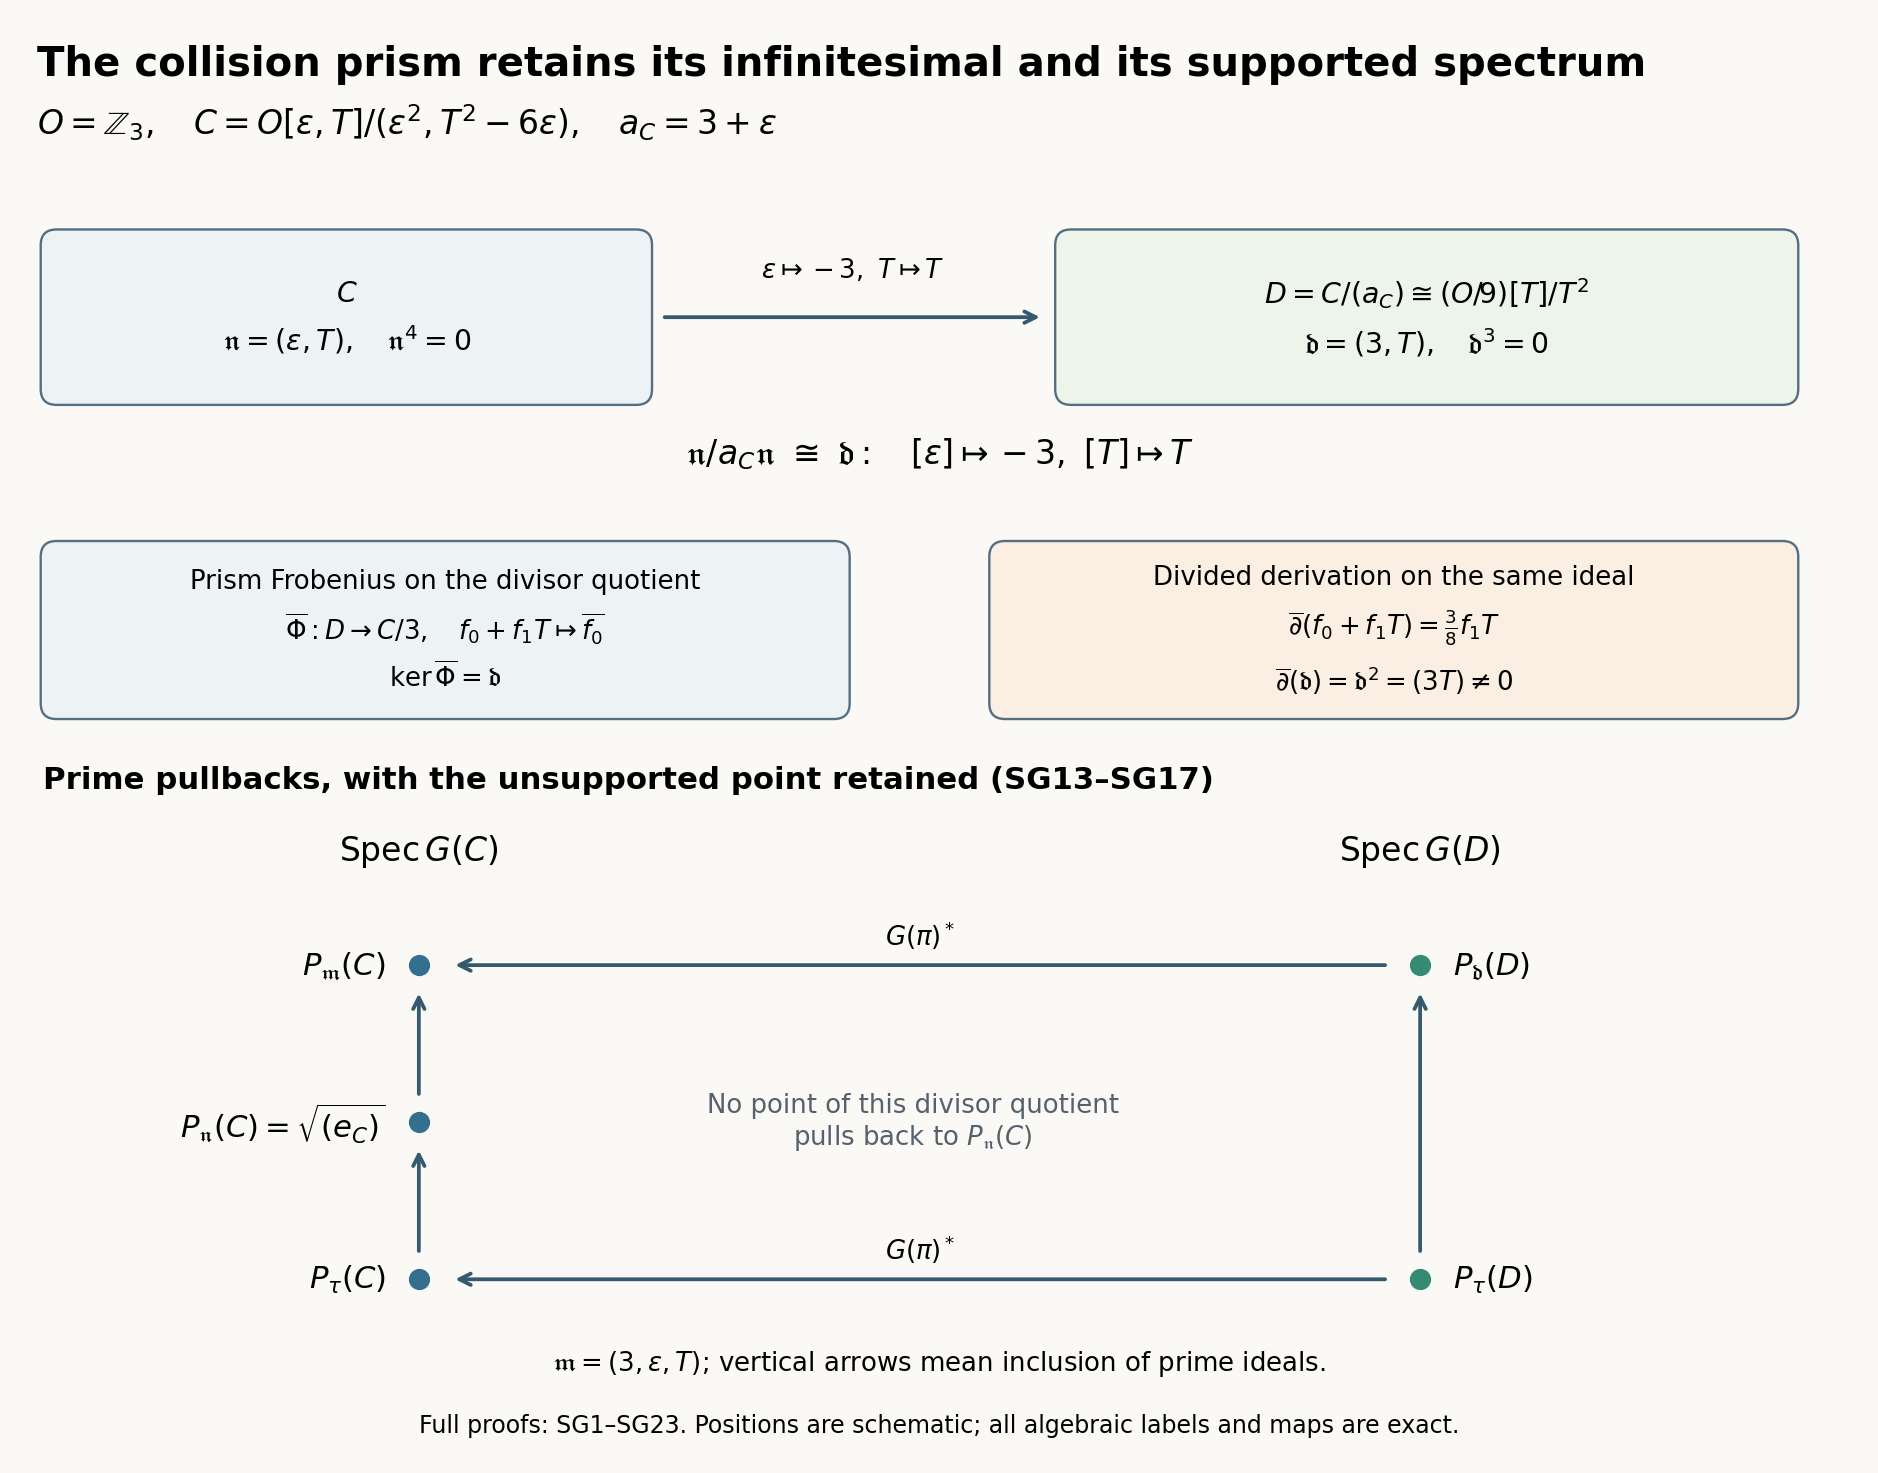
\includegraphics[keepaspectratio,alt={The divisor quotient and prime pullbacks, including the nonclosed supported image. The Frobenius kernel and divided-derivation image are ideals in the same ring. Full proofs SG13--SG23.}]{supported_collision_prism.png}}
\caption{The divisor quotient and prime pullbacks, including the
nonclosed supported image. The Frobenius kernel and divided-derivation
image are ideals in the same ring. Full proofs SG13--SG23.}
\end{figure}

\clearpage

\section{The global heat zero trace and its exact infinitesimal
variation}\label{the-global-heat-zero-trace-and-its-exact-infinitesimal-variation}

\textbf{Original-zeta receiving calculation.} The working meromorphic
function is the original Riemann zeta, with its full Gamma/endpoints
multiplier and its full trivial-zero and pole divisor retained.
\href{FAITHFUL_THETA_COMPLETION_RETURN.md}{TF1--42} proves the original
labelled theta inverse and the actual heat-image defect.
\href{FAITHFUL_UNCOMPLETED_ZETA_HEAT.md}{UZ1--53} proves every
exceptional-point fibre, jet, original-zeta heat term and reflection
orientation.
\href{ORIGINAL_ZETA_COMPACT_WEIL_RECONSTRUCTION.md}{OZC1--48} rederives
the compact contour and interval operator directly from zeta, including
the left-cutoff Gamma boundary, and specifies exactly which compensated
pairing the bounds concern.
\href{ORIGINAL_ZETA_HEAT_CONTACT_RECONSTRUCTION.md}{OZH1--49} rederives
the actual meromorphic heat, rational signed trace, compact-test domain,
contact drift and full causal arithmetic variation. The raw full divisor
and the compensated Weil receiver are linked by their displayed
correction, not identified. In particular the fixed-test trivial-zero
sum converges exactly at translations at least 1/32 and equals the
earlier R term; at zero translation it requires the proved cutoff
compensation. \href{ORIGINAL_ZETA_CAUCHY_RECONSTRUCTION.md}{OZK1--38}
reconstructs the original signed Cauchy trace, its full Gamma
correction, resonant finite parts, every finite matrix and its index,
and the complete local heat jets. Its invertible map retains the raw
trace and correction separately. These complete receiving proofs govern
the interpretation of the retained auxiliary calculations below.

This proof establishes an actual holomorphic family of global zero
traces for rational tests, and a separately specified regularized
variation for rapidly decreasing entire tests. The two domains and their
comparison maps are retained. The original heat family, constants and
supported endpoint coordinates are used throughout.

\subsection{1. Uniform growth of the original entire
family}\label{uniform-growth-of-the-original-entire-family}

Use the original Rodgers--Tao integral and coordinates \[
\begin{aligned}
H_t(Z)&=\int_0^\infty e^{tu^2}\Phi(u)\cos(Zu)\,du,\\
\Phi(u)&=\sum_{n\ge1}(2\pi^2n^4e^{9u}-3\pi n^2e^{5u})e^{-\pi n^2e^{4u}},\\
g_t(s)&=16H_t(-2i(s-1/2)),\quad g_0=2\xi_R,\quad
\partial_tg_t=\tfrac14g_t''.
\end{aligned}\tag{AG1}
\] The author source is
\href{https://arxiv.org/src/1801.05914v5}{Rodgers--Tao,
arXiv:1801.05914v5}, equations \texttt{hoz}, \texttt{phidef},
\texttt{htdef} and its subsequent heat equation. The coordinate
verification is also given directly in HA1--HA4 of this edition.

For \(u\ge0\), summing the defining series after retaining a fixed part
of its \(n^2\) exponent gives constants \(C,c>0\) with \[
|\Phi(u)|\le C e^{9u-ce^{4u}}.
\tag{AG2}
\] For example split \(\pi n^2e^{4u}\) into two equal parts. One is at
least \((\pi/2)e^{4u}\), and the other makes \(\sum n^4e^{-\pi n^2/2}\)
converge uniformly. The term with \(n^2e^{5u}\) has the same bound. For
each fixed \(T\), the function \(Tu^2-(c/2)e^{4u}\) is bounded above on
\([0,\infty)\). Thus on \(|t|\le T, |s|\le R\), the integral is bounded
by a constant depending on \(T\) times \[
\int_0^\infty \exp\bigl((2R+10)u-(c/2)e^{4u}\bigr)\,du
\le \exp(C_T(R+1)\log(R+2)).
\tag{AG3}
\] For the last inequality put \(x=e^{4u}\), enlarge the resulting
integral from \([1,\infty)\) to \([0,\infty)\), and use the Gamma
integral with exponent \((2R+10)/4\). Its positive-real Stirling bound
gives (AG3). Differentiating in \(s,t\) adds powers of \(u\), still
integrable by (AG2). Consequently \(g\) is jointly entire and has order
at most one in \(s\), uniformly on bounded time sets in the growth sense
of (AG3).

Every real time \(t_*\) has \(g_{t_*}(0)>0\). In fact \(\Phi(u)>0\)
termwise for \(u\ge0\), since \(2\pi n^2e^{4u}-3>0\), and the integral
at \(s=0\) uses \(\cosh u>0\). Continuity therefore supplies a complex
time disc about \(t_*\) on which \(g_t(0)\) stays bounded away from
zero. Jensen's formula on radii \(R\) and \(2R\), combined with (AG3),
gives the uniform zero count \[
N_t(R):=\sum_{|\rho|\le R}m_{\rho,t}=O(R\log(R+2)).
\tag{AG4}
\] The constant is uniform on a smaller closed time disc. Dyadic
summation gives the useful uniform tail estimate \[
\sum_{|\rho|>R}\frac{m_{\rho,t}}{|\rho|^2}
=O\left(\frac{\log(R+2)}R\right).
\tag{AG5}
\] No common vertical strip for the moving zeros has been assumed.

\subsection{2. A rational test has a finite-pole global
trace}\label{a-rational-test-has-a-finite-pole-global-trace}

Let \(A(s)\) be rational, with \(A(s)=O(s^{-2})\) at infinity. Fix a
real time \(t_*\) at which none of its finitely many poles is a zero of
\(g_{t_*}\). Compact continuity supplies a smaller complex time disc
\(D\) on which all those values and \(g_t(0)\) stay nonzero. Define \[
Z_t(A)=\sum_{g_t(\rho)=0}m_{\rho,t}A(\rho),\qquad t\in D.
\tag{AG6}
\] For each \(t\), the sum is absolutely convergent by (AG4)--(AG5). Its
far tail is uniformly bounded by \(C_A\log(R+2)/R\); fixed poles are
excluded by the choice of \(D\).

Hadamard factorization for an entire function of order at most one, with
the nonzero value at zero, gives \[
L_t(s):=g_t'(s)/g_t(s)
=\beta_t+\sum_\rho m_{\rho,t}
\left(\frac1{s-\rho}+\frac1\rho\right).
\tag{AG7}
\] The series is normally convergent away from the zeros. Its normal
convergence follows directly for the logarithmic derivative from
\(\sum m/|\rho|^2<\infty\), because the paired summand is
\(O_K(|\rho|^{-2})\) on a fixed compact set \(K\). The exponential
factor in the genus-one product supplies the constant \(\beta_t\).

Let \(\mathcal P(A)\) be the finite pole set of \(A\). The exact global
identity is \[
\boxed{Z_t(A)=-\sum_{p\in\mathcal P(A)}
\operatorname{Res}_{s=p}\bigl(A(s)L_t(s)\bigr).}
\tag{AG8}
\] To prove it, \(\sum_p\operatorname{Res}_pA=0\), since
\(A=O(s^{-2})\). Thus the constant \(\beta_t\) and each \(1/\rho\)
correction in (AG7) give zero after summing residues. For one zero
\(\rho\), the rational function \(A(s)/(s-\rho)\) has zero residue at
infinity, so its residues at the poles of \(A\) sum to \(-A(\rho)\).
Normal convergence on small circles around the finite pole set justifies
taking residues term by term. This proves (AG8), including repeated
poles of \(A\) and repeated zeros of \(g_t\).

The right side of (AG8) is holomorphic in \(t\) on \(D\). This proves
holomorphic dependence of the actual whole zero trace. In particular its
derivative is \[
\dot Z_t(A)=-\frac14\sum_{p\in\mathcal P(A)}
\operatorname{Res}_{s=p}\left(A(s)\partial_s\frac{g_t''(s)}{g_t(s)}\right).
\tag{AG9}
\] This conclusion does not exchange a derivative with an unrestricted
infinite moving-zero sum. The finite residue expression proves the
derivative of that sum as a holomorphic function.

\subsection{3. The Cauchy kernel and the original test
domain}\label{the-cauchy-kernel-and-the-original-test-domain}

For \(\Re z,\Re w>1\), set \[
F_z(s)=(s-z)^{-1},\quad F^\#(s)=\overline{F(1-\bar s)},\quad
A_{z,w}=F_z^\#F_w=-\frac1{(s-(1-\bar z))(s-w)}.
\tag{AG10}
\] At time zero both poles are nonzeros of \(g_0=2\xi_R\), by the
unconditional critical-strip result proved in SZW25. Formula (AG8) now
evaluates both simple residues: \[
Z_t(A_{z,w})=
\frac{L_t(w)-L_t(1-\bar z)}{w+\bar z-1}
=\frac{L_t(w)+L_t(\bar z)}{w+\bar z-1}.
\tag{AG11}
\] Reflection gives the second equality for complex time. For real time
\(L_t(\bar z)=\overline{L_t(z)}\). For a fixed finite set of tests the
time disc is common to all its poles. If \(z,w>1\) are real, the
positive integral and reflection make their poles nonzeros at every real
time, so the same local argument applies around any such time.

The minus-exponent Mellin convention is the original one: \[
M_h(s)=\int_{\mathbb R}h(u)e^{-(s-1/2)u}\,du.
\tag{AG12}
\] For (AG10) its inverse is exactly \[
h_{z,w}(u)=\frac1{w+\bar z-1}
\begin{cases}e^{-(\bar z-1/2)u},&u\ge0,\\
e^{(w-1/2)u},&u\le0.
\end{cases}
\tag{AG13}
\] Direct integration proves (AG12) on \(1-\Re z<\Re s<\Re w\). The
values at zeros outside this strip at other times use the rational
meromorphic continuation (AG10); this is not an enlargement of the
domain of convergence of the integral.

More generally take any rational \(A=O(s^{-2})\) whose poles all lie in
\(\Re s<0\) or \(\Re s>1\). Its inverse on the critical line has the
explicit residue representation \[
h_A(u)=
\begin{cases}
\displaystyle\sum_{\Re p<0}\operatorname{Res}_{s=p}
\left(e^{(s-1/2)u}A(s)\right),&u\ge0,\\
\displaystyle-\sum_{\Re p>1}\operatorname{Res}_{s=p}
\left(e^{(s-1/2)u}A(s)\right),&u\le0.
\end{cases}
\tag{AG14}
\] Partial fractions and integration of exponential polynomials verify
this directly. At zero the two expressions agree because the finite
residues of \(A\) sum to zero. There is \(d>1/2\) such that \(h_A\), its
first derivative on the two half-lines and its distributional second
derivative have finite weighted norms with weight \(e^{d|u|}\); for the
second derivative the norm means total variation of a measure. The
possible derivative jump contributes one delta atom. Repeated poles
produce only polynomial factors multiplying the decreasing exponentials
and do not affect this conclusion after decreasing \(d\) slightly.

Let \(h_{R,\varepsilon}\) be a smooth compact cutoff of \(h_A\) on
\([-R-1,R+1]\), convolved with a smooth mollifier of radius
\(\varepsilon\to0\). The first two cutoff derivatives can be bounded
independently of \(R\). Consequently the weighted norms just stated
remain bounded uniformly for \(R\ge1,\varepsilon\le1\). Distributional
integration by parts twice gives \[
|M_{h_{R,\varepsilon}}(\sigma+iy)|\le\frac{C}{1+y^2}
\quad(0\le\sigma\le1),\qquad
|h_{R,\varepsilon}(u)|\le Ce^{-d|u|}.
\tag{AG15}
\] For the latter inequality apply the fundamental theorem of calculus
to the absolutely continuous weighted function, using the bounded
weighted value and first-derivative norms. The transforms converge
pointwise to \(A\) on the strip. The zero sum is dominated by
\(\sum m/(1+|\Im\rho|^2)<\infty\), from SZW25 and (AG4). The prime sum
is dominated by \(C\sum\Lambda(n)n^{-1/2-d}<\infty\), and the
archimedean integrand by \(C\log(2+|y|)/(1+y^2)\). Endpoint convergence
follows from the weighted \(L^1\) bound. Applying dominated convergence
to the complete compact-test formula SZW25 therefore proves its
extension to \(h_A\), with all its terms.

In particular, for \(A=A_{z,w}\), the exact supported identity remains
\[
\begin{aligned}
\boldsymbol B_L&=(A(0)+A(1))\mathbf e_{1_L}
+A(0)\sum_{\lambda\ne1_L}\mathbf e_\lambda,\\
\boldsymbol Z_L&=Z_0(A)\mathbf e_{1_L},\\
\boldsymbol D_L&=(P_{\rm fin}(h_A)-A_\infty(h_A))\mathbf e_{1_L}
+A(0)\sum_{\lambda\ne1_L}\mathbf e_\lambda,\\
\boldsymbol B_L-\boldsymbol Z_L&=\boldsymbol D_L.
\end{aligned}\tag{AG16}
\] These are the original SZW representations and label maps. Explicit
evaluation of each Cauchy term and its actual heat derivative is proved
in HA10--HA20.

\subsection{4. Every finite collision has an exact contour
derivative}\label{every-finite-collision-has-an-exact-contour-derivative}

Let \(\rho\) be any actual zero of \(g_0\), of multiplicity \(m\), and
write \(g_0(s)=(s-\rho)^mu_\rho(s)\), \(u_\rho(\rho)\ne0\). A small
fixed circle containing only this zero has no zeros on its boundary for
small complex time. For every test \(A\) holomorphic near its closed
disc, the argument principle gives the cluster trace and derivative \[
Z_{\rho,t}(A)=\frac1{2\pi i}\int_{\partial D_\rho}A(s)L_t(s)\,ds,
\quad
\dot Z_{\rho,0}(A)
=-\frac{m(m-1)}4A''(\rho)
-\frac m2\frac{u_\rho'(\rho)}{u_\rho(\rho)}A'(\rho).
\tag{AG17}
\] Indeed \(g_0''/(4g_0)\) has principal part
\(m(m-1)/(4(s-\rho)^2)+(m/2)(u_\rho'/u_\rho)(\rho)/(s-\rho)\).
Differentiate this principal part in \(s\), multiply by the Taylor
expansion of \(A\), and take its residue. Compact nonvanishing on the
fixed circle permits the time derivative. No derivative of an
individually labelled colliding root is required.

\subsection{5. An entire-test variation with its exact
regularization}\label{an-entire-test-variation-with-its-exact-regularization}

For this section let \(A\) be entire and assume, for every integer
\(N\ge0\) and \(j=0,1,2\), \[
\sup_{0\le\Re s\le1}(1+|\Im s|)^N|A^{(j)}(s)|<\infty.
\tag{AG18}
\] This includes original compactly supported smooth Mellin tests by
repeated integration by parts. The zeros in this section are the
distinct zeros of \(g_0\), with multiplicities \(m_\rho\); they lie
strictly inside the critical strip. Put \(b=g_0'(0)/g_0(0)\), and for
distinct zeros define \[
T_A(\rho,\eta)=\frac{A'(\rho)-A'(\eta)}{\rho-\eta}
+\frac{A'(\rho)}\eta+\frac{A'(\eta)}\rho.
\tag{AG19}
\] The following expression is absolutely convergent: \[
\begin{aligned}
\mathcal V(A)=-\frac14\Bigg[&\sum_\rho m_\rho(m_\rho-1)A''(\rho)
+2b\sum_\rho m_\rho A'(\rho)
+2\sum_\rho\frac{m_\rho^2A'(\rho)}\rho\\
&+2\sum_{\{\rho,\eta\}}m_\rho m_\eta T_A(\rho,\eta)\Bigg].
\end{aligned}\tag{AG20}
\] The last sum is over unordered pairs. To verify convergence, arrange
\(r=|\rho|\le R=|\eta|\). For \(R<2r\), either the distance is at least
\(r/2\), when direct rapid-decrease estimates apply, or the straight
segment joining them stays at modulus at least \(r/2\). In the second
case its real part stays inside the strip and
\((A'(\rho)-A'(\eta))/(\rho-\eta)=\int_0^1A''(\eta+t(\rho-\eta))dt\).
Thus \(|T_A|\le C_N(1+r)^{-N}\). The total multiplicity weight of
comparable pairs in a dyadic annulus is \(O(r^2\log^2(2+r))\), which is
summable for large \(N\).

If \(R\ge2r\), retain the exact cancellation \[
T_A(\rho,\eta)=\frac{\rho A'(\rho)}{\eta(\rho-\eta)}
+\frac{\eta A'(\eta)}{\rho(\eta-\rho)},\quad
|T_A|\le\frac{2r|A'(\rho)|}{R^2}+\frac{2|A'(\eta)|}r.
\tag{AG21}
\] The zero count gives
\(\sum_{|\eta|\ge R}m_\eta/|\eta|^2=O(\log(2+R)/(1+R))\) and
\(\sum_{|\rho|\le R}m_\rho/|\rho|=O(\log^2(2+R))\). These bounds and
(AG18) prove convergence of the disparate-pair sum. The single sums in
(AG20) converge as well, using the bound on \(\sum m_\rho^2\) in an
annulus by the square of its total multiplicity. Finitely many zeros
near the origin cause no problem since \(g_0(0)\ne0\).

Here is the precise relation of (AG20) to the original family. For every
sufficiently large integer \(j\), select \(T_j\in[j,j+1]\) at distance
at least \(j^{-3}\) from every \(|\Im\rho|\). Such a value exists: only
zeros of modulus at most \(2j+4\) matter, and their excluded intervals
have total length \(O(j^{-2}\log j)<1\). Let \(\Gamma_j\) be the
rectangle with real edges \(-1,2\) and heights \(\pm T_j\). For each
fixed \(j\), its zero trace is analytic for sufficiently small time.
Then \[
\boxed{\mathcal V(A)=\lim_{j\to\infty}
\left.\frac d{dt}\right|_0\frac1{2\pi i}\int_{\Gamma_j}A(s)L_t(s)\,ds.}
\tag{AG22}
\] To prove it, expand the regular part of (AG7) at \(\rho\): \[
\frac{u_\rho'(\rho)}{u_\rho(\rho)}
=b+\frac{m_\rho}\rho+
\sum_{\eta\ne\rho}m_\eta\left(\frac1{\rho-\eta}+\frac1\eta\right).
\tag{AG23}
\] The series converges for this fixed zero by genus-one cancellation.
Insert it in (AG17), summed over zeros inside \(\Gamma_j\). Pairs both
inside combine to (AG19). The remaining cross-boundary sum is \[
E_T=\sum_{|\Im\rho|<T<|\Im\eta|}
m_\rho m_\eta A'(\rho)
\left(\frac1{\rho-\eta}+\frac1\eta\right).
\tag{AG24}
\] For \(|\rho|\le T/2\) its absolute value is \(O(\log T/T)\), by the
paired tail bound and summability of \(m_\rho|\rho A'(\rho)|\). For
\(T/2<|\rho|\le2T\), \(T\le|\eta|\le4T\), the separated height gives
\(|\rho-\eta|\gg T^{-3}\); the total is \(O_N(T^{5-N}\log^2T)\). For the
same \(\rho\) and \(|\eta|>4T\), genus-one cancellation bounds the sum
by \(O_N(T^{1-N}\log^2T)\). Hence \(E_T\to0\). Absolute convergence of
(AG20) now proves (AG22) and independence from the chosen separated
exhaustion.

Formula (AG22) is a contour-regularized global variation: it is the
limit of the derivatives of finite traces, with its order of operations
specified. It does not assert that arbitrary entire tests in (AG18) have
a holomorphic global moving-zero sum at nearby times. The stronger
statement for rational tests is (AG6)--(AG9), proved by their finite
pole map. Both receivers retain their exact domains rather than being
identified without a convergence argument.

\subsection{Sources and receiving
calculations}\label{sources-and-receiving-calculations}

The exact original heat source and original author equations are cited
at (AG1). Classical Jensen and Hadamard theorems are used with their
growth and nonvanishing hypotheses verified in (AG2)--(AG7). The
complete original supported formula and its zero-count and prime-contour
proofs are
\href{https://github.com/KokunoYumeto/zeta-function-research-reader/blob/3c022a0adde0a6aa3d8fc8e43ef42795d88e44b0/workbenches/splitzero-tandem/branches/tau-zero-prime-positivity/SUPPORTED_ZERO_PRIME_WEIL_DERIVATION.md}{SZW19--SZW38}.
Its human Connes attribution and original source convention are
retained. HA applies (AG8) to the complete arithmetic variation; HM
applies it to all time derivatives; the Cauchy--Weil criterion applies
(AG11) at zero. No assertion of RH or its negation follows from
convergence alone.

\subsection{Actual positive-real-time
continuation}\label{actual-positive-real-time-continuation}

The complete \href{REAL_TIME_HEAT_TRACE_DERIVATION.md}{real-time proof},
RT1--30, strengthens the compact-test variation in this edition: the
whole zero trace is smooth for the original real heat time t at least
zero, with actual right derivatives at zero. RT16 identifies its first
derivative with the full causal arithmetic distribution, and RT20--27
constructs every higher meromorphic derivative receiver. The contact
comparison retains the unit and inter-zero terms. These results do not
assert a common zero strip for negative or complex time and do not prove
the remaining RH inequality. All original supported carriers remain
present.

\clearpage

\section{The actual heat pairing, its supported endpoints, and mixed
prime
products}\label{the-actual-heat-pairing-its-supported-endpoints-and-mixed-prime-products}

\textbf{Original-zeta receiving calculation.} The working meromorphic
function is the original Riemann zeta, with its full Gamma/endpoints
multiplier and its full trivial-zero and pole divisor retained.
\href{FAITHFUL_THETA_COMPLETION_RETURN.md}{TF1--42} proves the original
labelled theta inverse and the actual heat-image defect.
\href{FAITHFUL_UNCOMPLETED_ZETA_HEAT.md}{UZ1--53} proves every
exceptional-point fibre, jet, original-zeta heat term and reflection
orientation.
\href{ORIGINAL_ZETA_COMPACT_WEIL_RECONSTRUCTION.md}{OZC1--48} rederives
the compact contour and interval operator directly from zeta, including
the left-cutoff Gamma boundary, and specifies exactly which compensated
pairing the bounds concern.
\href{ORIGINAL_ZETA_HEAT_CONTACT_RECONSTRUCTION.md}{OZH1--49} rederives
the actual meromorphic heat, rational signed trace, compact-test domain,
contact drift and full causal arithmetic variation. The raw full divisor
and the compensated Weil receiver are linked by their displayed
correction, not identified. In particular the fixed-test trivial-zero
sum converges exactly at translations at least 1/32 and equals the
earlier R term; at zero translation it requires the proved cutoff
compensation. \href{ORIGINAL_ZETA_CAUCHY_RECONSTRUCTION.md}{OZK1--38}
reconstructs the original signed Cauchy trace, its full Gamma
correction, resonant finite parts, every finite matrix and its index,
and the complete local heat jets. Its invertible map retains the raw
trace and correction separately. These complete receiving proofs govern
the interpretation of the retained auxiliary calculations below.

This calculation uses the original heat family and the full
supported-zero explicit formula. It gives an actual global family of
pairings and computes its arithmetic derivative. Positivity of that
family at time zero is not assumed. All lower support coordinates remain
in the formula.

\subsection{1. Original family and
coordinates}\label{original-family-and-coordinates}

Write \(\xi_R(s)=\tfrac12s(s-1)\pi^{-s/2}\Gamma(s/2)\zeta(s)\). The
original Rodgers--Tao conventions are \[
\begin{aligned}
\Phi(u)&=\sum_{n\ge1}(2\pi^2n^4e^{9u}-3\pi n^2e^{5u})e^{-\pi n^2e^{4u}},\\
H_t(Z)&=\int_0^\infty e^{tu^2}\Phi(u)\cos(Zu)\,du,\\
H_0(Z)&=\tfrac18\xi_R(\tfrac12+iZ/2),\qquad
\partial_tH_t=-\partial_Z^2H_t.
\end{aligned}\tag{HA1}
\] These are the original source equations \texttt{phidef},
\texttt{htdef}, \texttt{hoz}, and the sentence following \texttt{htdef}
in \href{https://arxiv.org/src/1801.05914v5}{Rodgers--Tao,
arXiv:1801.05914v5, author TeX}. Define, retaining the factor 16 and the
coordinate factor \(-2i\), \[
g_t(s)=16H_t(-2i(s-\tfrac12)),\qquad g_0(s)=2\xi_R(s),
\qquad L_t(s)=\frac{\partial_sg_t(s)}{g_t(s)}.
\tag{HA2}
\] The superexponential decrease in (HA1) makes the integral and all its
derivatives converge uniformly on compact subsets of
\(\mathbb C_t\times\mathbb C_s\). For example, on \(|t|\le T,|s|\le R\),
its integrand is bounded by a constant times
\(\exp(Tu^2+2(R+1)u+9u-ce^{4u})\), an integrable function; derivatives
add only polynomial factors in \(u\). It follows by differentiation that
\[
\partial_tg_t=\tfrac14\partial_s^2g_t,\qquad
\partial_tL_t=\tfrac14\partial_s\left(\frac{g_t''}{g_t}\right)
=\tfrac14(L_t''+2L_tL_t').
\tag{HA3}
\] The factor \(1/4\) follows because \((-2i)^2=-4\). For every complex
\(t\), \(g_t(1-s)=g_t(s)\). For real \(t\),
\(g_t(\bar s)=\overline{g_t(s)}\). Thus \[
L_t(1-s)=-L_t(s),\qquad
L_t(\bar s)=\overline{L_t(s)}\quad(t\in\mathbb R).
\tag{HA4}
\] These identities hold wherever the displayed quotients are defined.

\subsection{2. The Cauchy tests in the original Mellin
convention}\label{the-cauchy-tests-in-the-original-mellin-convention}

Let \(z,w\in\mathcal U=\{s:\Re s>1\}\), and put \[
q=w+\bar z-1,\qquad F_z(s)=\frac1{s-z},\qquad
A_{z,w}(s)=F_z^\#(s)F_w(s)
=-\frac1{(s-(1-\bar z))(s-w)},
\tag{HA5}
\] where \(F^\#(s)=\overline{F(1-\bar s)}\). In particular, \(\Re q>1\),
and both poles lie strictly outside the closed critical strip. The exact
original inverse Mellin tests are \[
f_z(u)=-1_{(-\infty,0]}(u)e^{(z-1/2)u},\qquad
h_{z,w}=f_z^\#*f_w,
\tag{HA6}
\] with time-domain involution \(f^\#(u)=\overline{f(-u)}\). Direct
integration gives \[
h_{z,w}(u)=\frac1q
\begin{cases}
e^{-(\bar z-1/2)u},&u\ge0,\\
e^{(w-1/2)u},&u\le0,
\end{cases}
\quad
A_{z,w}(s)=\int_{\mathbb R}h_{z,w}(u)e^{-(s-1/2)u}\,du.
\tag{HA7}
\] The second identity initially holds for \(1-\Re z<\Re s<\Re w\),
including the closed critical strip; it then gives the meromorphic
expression (HA5). The function \(h\) is continuous at zero, and its
derivative jump is exactly \(-1\). Its distributional second derivative
is the sum of two exponentially decreasing functions and \(-\delta_0\).
Neither this atom in the test derivative nor the supported-zero point is
identified with the unsupported element \(\tau\).

The complete extension of the compact-test explicit formula to these
tests is proved in \href{ACTUAL_HEAT_ZERO_DISTRIBUTION_VARIATION.md}{the
global heat zero-distribution calculation}. Here is also the needed
convergence argument. Choose \(d\) strictly between \(1/2\) and
\(\min(\Re z,\Re w)-1/2\). Cut \(h\) off with a smooth function equal to
one on \([-R,R]\) and zero outside \([-R-1,R+1]\), and convolve with a
smooth approximate identity of radius \(\varepsilon_R\le1\), where
\(\varepsilon_R\to0\) as \(R\to\infty\). The resulting smooth compact
tests have uniformly bounded weighted \(L^1\) norms of their value and
first derivative and uniformly bounded weighted total variation of the
second derivative, with weight \(e^{d|u|}\). This follows directly from
(HA7), its derivative jump, the bounded cutoff derivatives and the
compact support of the mollifier. Their transforms therefore obey a
uniform bound \(C/(1+|y|^2)\) for \(0\le\Re s\le1\), by distributional
integration by parts twice. Their pointwise limits give \(A\). The
unconditional zero count \(N(R)=O(R\log(2+R))\), already proved in
SZW25, makes the zero sums uniformly summable. The prime sum is
dominated by \(C\sum\Lambda(n)n^{-1/2-d}\), and the archimedean integral
by \(C\log(2+|y|)/(1+y^2)\). Endpoints converge by the same weighted
\(L^1\) estimate. Thus dominated convergence applies to every term of
SZW25, retaining both endpoints and every support label.

\subsection{3. Exact global pairing and all arithmetic terms at
zero}\label{exact-global-pairing-and-all-arithmetic-terms-at-zero}

Zeros are counted with their multiplicities. The rational zero trace is
\[
K_t(z,w)=\sum_{g_t(\rho)=0}m_\rho A_{z,w}(\rho).
\tag{HA8}
\] For each fixed finite set of \(z,w\) there is a complex time disc
around zero in which no pole of its tests is a zero of \(g_t\). The full
global Hadamard argument in
\href{ACTUAL_HEAT_ZERO_DISTRIBUTION_VARIATION.md}{the zero-distribution
calculation} proves convergence and holomorphic dependence on that disc,
and gives \[
K_t(z,w)=\frac{L_t(w)-L_t(1-\bar z)}q
=\frac{L_t(w)+L_t(\bar z)}q.
\tag{HA9}
\] For real time the numerator is \(L_t(w)+\overline{L_t(z)}\). The
proof can be seen directly from the genus-one logarithmic derivative:
subtract its values at the two poles. The constant term and each
\(1/\rho\) correction cancel; the remaining summand divided by \(q\) is
exactly (HA5) at \(\rho\). Absolute convergence follows from
\(A(\rho)=O(|\rho|^{-2})\) and the uniform zero count. Multiplicities
are retained in this argument.

Introduce three distinct functions on \(\Re s>1\): \[
\begin{aligned}
e_0(s)&=\frac1s+\frac1{s-1},\\
b(s)&=-\tfrac12\log\pi+\tfrac12\psi(s/2),\\
r(s)&=\frac{\zeta'(s)}{\zeta(s)}=-\sum_{n\ge2}\Lambda(n)n^{-s}.
\end{aligned}\qquad L_0=e_0+b+r.
\tag{HA10}
\] The notation \(e_0(s)\) is a scalar logarithmic-derivative function,
not the programme element \(e\). The endpoint, archimedean and
finite-prime values for (HA7) are, separately, \[
\begin{aligned}
E(z,w)&=A_{z,w}(0)+A_{z,w}(1)
=\frac1{w(\bar z-1)}+\frac1{\bar z(w-1)}
=\frac{e_0(w)+\overline{e_0(z)}}q,\\
G(z,w)&=\frac{b(w)+\overline{b(z)}}q,\\
P(z,w)&=\frac1q\sum_{n\ge2}\Lambda(n)(n^{-w}+n^{-\bar z})
=-\frac{r(w)+\overline{r(z)}}q,\\
K_0(z,w)&=E(z,w)+G(z,w)-P(z,w).
\end{aligned}\tag{HA11}
\] The endpoint equality follows by common denominators, and the prime
equality follows from (HA7) in SZW24. For completeness, the Gamma
equality has a direct integral proof. The convergent digamma
representation for \(\Re a>0\) is \[
\psi(a)=-\gamma+\int_0^\infty
\frac{e^{-x}-e^{-ax}}{1-e^{-x}}\,dx.
\tag{HA12}
\] It follows from the logarithmic derivative of Euler's product for
Gamma: expand \((1-e^{-x})^{-1}\), integrate finite partial sums, and
use the cancellation at zero to obtain
\(-\gamma+\sum_{j\ge0}(1/(j+1)-1/(j+a))\). With the original Fourier
convention, the archimedean integral is consequently \[
\begin{aligned}
A_\infty(h)=&-(\gamma+\log\pi)h(0)\\
&+\int_0^\infty\frac{e^{-x}h(0)-\frac12e^{-x/4}(h(x/2)+h(-x/2))}{1-e^{-x}}\,dx.
\end{aligned}\tag{HA13}
\] One may first truncate the \(x\) integral. Fourier inversion then
proves the identity. Passing to the limit is legitimate: at zero the
numerator is \(O(x)\) by the Lipschitz property of \(h\), and at
infinity it decreases exponentially. On the Fourier side, the truncated
integrals are bounded by \(C\log(2+|y|)\), uniformly in the cutoffs. To
verify that bound, split at \(x=1/(1+|y|)\) and at 1 and use
\(|1-\cos(yx/2)|\le\min(2,y^2x^2/8)\). The remaining nonoscillatory
difference is integrable independently of \(y\). The bound on
\(A(1/2+iy)\) proved above supplies domination. Substituting (HA7) in
(HA13) gives (HA11) by (HA12), with every factor \(1/2\) retained.

Let \(L\) now denote the finite support semilattice of SZW, with top
\(1_L\); this is distinct from the function \(L_t(s)\). In the unchanged
vector space with coordinate basis \(\mathbf e_\lambda\), the full
identity is \[
\begin{aligned}
\boldsymbol B_L(z,w)&=E(z,w)\mathbf e_{1_L}
+A_{z,w}(0)\sum_{\lambda\ne1_L}\mathbf e_\lambda,\\
\boldsymbol Z_L(0;z,w)&=K_0(z,w)\mathbf e_{1_L},\\
\boldsymbol D_L(0;z,w)&=(P(z,w)-G(z,w))\mathbf e_{1_L}
+A_{z,w}(0)\sum_{\lambda\ne1_L}\mathbf e_\lambda,\\
\boldsymbol B_L-\boldsymbol Z_L(0)&=\boldsymbol D_L(0).
\end{aligned}\tag{HA14}
\] This is exactly SZW33--34 evaluated on (HA7). In particular, the
lower fixed traces have not been dropped. Summing all coordinates and
projecting to the top coordinate are different maps with the kernels
proved in SZW35--37. The coefficient of each lower coordinate is
generally not a Hermitian form by itself. The Hermitian positivity
question below concerns the full reflected zero trace \(K_0\), as in
SZW32 and SZW38, with (HA14) giving its exact supported arithmetic
realization.

\subsection{4. The actual derivative and its mixed prime
products}\label{the-actual-derivative-and-its-mixed-prime-products}

Set \(a=e_0+b\), and define \(v=a'+a^2\). For \(\Re s>1\), the exact
series is \[
\frac{g_0''}{g_0}(s)
=v(s)+\sum_{n\ge2}\bigl[\Lambda(n)\log n+(\Lambda*\Lambda)(n)-2a(s)\Lambda(n)\bigr]n^{-s},
\tag{HA15}
\] where \((\Lambda*\Lambda)(n)=\sum_{d\mid n}\Lambda(d)\Lambda(n/d)\)
is ordered Dirichlet convolution. Indeed \(g_0''/g_0=L_0'+L_0^2\), and
inserting (HA10) gives (HA15). Each series, each required derivative and
each product converges absolutely and locally uniformly on \(\Re s>1\),
because \(\Lambda(n)\le\log n\) and \(\sum (\log n)^j n^{-c}<\infty\)
for every fixed \(c>1\).

It follows that the genuine time derivative is \[
\begin{aligned}
J(s):=\left.\partial_tL_t(s)\right|_{t=0}
=\frac14v'(s)+\frac14\sum_{n\ge2}C_n(s)n^{-s},\\
C_n(s)=-\Lambda(n)(\log n)^2-(\Lambda*\Lambda)(n)\log n
-2a'(s)\Lambda(n)+2a(s)\Lambda(n)\log n.
\end{aligned}\tag{HA16}
\] This includes the endpoint--Gamma and endpoint--prime cross terms in
\(a\), not merely a heat deformation of the old prime weights. Equations
(HA3) and (HA9) yield the exact global derivative \[
\boxed{\left.\partial_tK_t(z,w)\right|_{t=0}
=\frac{J(w)+\overline{J(z)}}{w+\bar z-1}.}
\tag{HA17}
\] It is a derivative of the actual infinite zero trace, not only a
derivative of a finite set of zeros. The holomorphic finite-pole formula
(HA9) supplies the justification; no unproved interchange with a moving
infinite zero sum is used.

There is a useful exact distinction among arithmetic indices. If
\(n=p^k\), then \[
\Lambda(n)\log n+(\Lambda*\Lambda)(n)
=(2k-1)(\log p)^2.
\tag{HA18}
\] The \(k-1\) ordered proper prime-power factorizations give the
convolution. If \(n=p^\alpha q^\beta\), where \(p\ne q\) and
\(\alpha,\beta\ge1\), then \[
\Lambda(n)=0,\quad (\Lambda*\Lambda)(n)=2\log p\log q,
\quad \frac14C_n(s)=-\frac12\log p\log q\log(p^\alpha q^\beta).
\tag{HA19}
\] These are the two possible ordered factorizations into prime powers.
With three or more distinct prime divisors both functions vanish. Thus
the first actual heat derivative already contains products of two
distinct prime contributions. Formula (HA19) does not arise from
replacing an ordinary prime by a new numerical norm for supported zero.
It is forced by the nonlinear term \(2L_0L_0'\) in the exact evolution.

To retain the whole support vector through this calculation, let
\(\Lambda_t(s)=g_t(s)/(s(s-1))\). At real time close to zero this
function has simple poles at zero and one, since \(g_0(0)=g_0(1)=1\) and
compact continuity keeps both values nonzero. Its logarithmic derivative
is \(L_t-e_0\), with residue \(-1\) at each pole. Their residues as
poles of \(\Lambda_t\) itself are \(-g_t(0)\) and \(g_t(1)\), and may
vary; these two statements are distinct.

The logarithmic-divisor receiver at time \(t\) therefore has unchanged
fixed endpoint weights and explicitly computed top coefficient \[
\begin{aligned}
\boldsymbol Z_L(t)&=K_t\mathbf e_{1_L},\\
\boldsymbol D_L(t)&=\left(E-\frac{L_t(w)+L_t(\bar z)}q\right)\mathbf e_{1_L}
+A_{z,w}(0)\sum_{\lambda\ne1_L}\mathbf e_\lambda,\\
\boldsymbol B_L-\boldsymbol Z_L(t)&=\boldsymbol D_L(t),\\
\dot{\boldsymbol D}_L(0)&=-\frac{J(w)+\overline{J(z)}}q\mathbf e_{1_L},
\qquad \dot{\boldsymbol B}_L=0.
\end{aligned}\tag{HA20}
\] Here the first two lines are evaluated from the actual meromorphic
heat function and its divisor. At zero, (HA11) identifies them with the
original arithmetic formula; (HA16) computes their arithmetic first
variation. No Euler product for \(g_t\) at nonzero time, or new
theta-cohomology identification at such time, is asserted. The lower
fixed distributions are the same explicit representations used in SZW,
and their zero derivative is a calculation for these fixed tests, not a
deletion of those distributions.

\subsection{5. Exact relation to a colliding
infinitesimal}\label{exact-relation-to-a-colliding-infinitesimal}

Fix any actual zero \(\rho\) of \(g_0\), of multiplicity \(m\), and
write \(g_0(s)=(s-\rho)^m u(s)\), \(u(\rho)\ne0\). On a small circle
enclosing just this cluster, the residue theorem gives its weighted
trace. Differentiating that fixed contour using (HA3) gives \[
\left.\partial_t Z_{\rho,t}(A)\right|_0
=-\frac{m(m-1)}4 A''(\rho)
-\frac m2\frac{u'(\rho)}{u(\rho)}A'(\rho).
\tag{HA21}
\] For proof, \(g_0''/(4g_0)\) has principal part
\(\frac{m(m-1)}4(s-\rho)^{-2}+\frac m2(u'/u)(\rho)(s-\rho)^{-1}\). Its
derivative has residue against \(A\) equal to the displayed expression.
The contour derivative exists without choosing or differentiating
individual colliding roots. Formula (HA21) retains the full analytic
unit.

For a critical-line zero \(\rho=1-\bar\rho\), take local tests \(F,G\)
vanishing at \(\rho\) and put \(A=F^\#G\). Then \(A'(\rho)=0\) and
\(A''(\rho)=-2\overline{F'(\rho)}G'(\rho)\). Hence \[
\left.\partial_t Z_{\rho,t}(F^\#G)\right|_0
=\frac{m(m-1)}2\overline{F'(\rho)}G'(\rho).
\tag{HA22}
\] This is the exact positive first response on the first vanishing-jet
layer of a critical collision. At an exchanged pair \(\rho,\rho^\#\),
the same calculation gives the cross pairing of the two derivative
values; its Gram matrix is a positive multiple of
\(\begin{psmallmatrix}0&1\\1&0\end{psmallmatrix}\), provided both tests
vanish at both points and \(m\ge2\). Thus the actual first response
preserves the distinction between a critical fixed point and an
exchanged pair. If \(m=1\), this particular first-jet response vanishes,
while (HA21) still retains the unit-dependent term for arbitrary tests.

For a finite rational test span \(F=\sum_j c_jF_{z_j}\), the global
quadratic form and derivative are exactly \[
Z_t(F^\#F)=\sum_{i,j}\bar c_iK_t(z_i,z_j)c_j,
\qquad
\left.\partial_t Z_t(F^\#F)\right|_0
=\sum_{i,j}\bar c_i\frac{J(z_j)+\overline{J(z_i)}}{z_j+\bar z_i-1}c_j.
\tag{HA23}
\] Every zero and every endpoint is retained by (HA8) and (HA14). A sign
on (HA22), or on a coefficient of (HA19), does not assign a sign to
(HA23). The complete criterion for the latter family at zero is proved
in \href{CAUCHY_WEIL_POSITIVITY_CRITERION.md}{Cauchy--Weil positivity}.

\subsection{6. A positive actual diagonal response and its precise
scope}\label{a-positive-actual-diagonal-response-and-its-precise-scope}

The kernel permits an unconditional sign calculation on the real
diagonal. For every real \(t\), \(\sigma>1\), put \(v=\sigma-1/2>0\) and
give \([0,\infty)\) the probability measure \[
d\mu_{t,v}(u)=\frac{e^{tu^2}\Phi(u)\cosh(2vu)\,du}{\int_0^\infty e^{ty^2}\Phi(y)\cosh(2vy)\,dy}.
\tag{HA24}
\] The measure is positive: every summand of \(\Phi(u)\) is
\(\pi n^2e^{5u}(2\pi n^2e^{4u}-3)e^{-\pi n^2e^{4u}}>0\) for \(u\ge0\).
Its density is strictly positive and all moments exist. Differentiation
of the actual integral (HA1), with the compact domination already
proved, gives \[
L_t(\sigma)=2\,\mathbb E_{\mu_{t,v}}[u\tanh(2vu)]>0,
\quad
\partial_tL_t(\sigma)=2\operatorname{Cov}_{\mu_{t,v}}(u^2,u\tanh(2vu))>0.
\tag{HA25}
\] For the second identity differentiate a normalized integral. Its
strict sign follows from \[
2\operatorname{Cov}(f,g)=\iint(f(u)-f(y))(g(u)-g(y))\,d\mu(u)d\mu(y).
\tag{HA26}
\] Both \(u^2\) and \(u\tanh(2vu)\) are strictly increasing on
\((0,\infty)\). The integrand is positive away from the diagonal, and
the positive continuous density gives positive mass to two disjoint
intervals. Thus the covariance is strictly positive, not merely
nonnegative.

Consequently \(K_t(\sigma,\sigma)=2L_t(\sigma)/(2\sigma-1)>0\) and its
actual time derivative is strictly positive for every real time. The
rational trace identity applies at every such fixed real time: its two
real poles are not zeros because the same positive integral makes
\(g_t(\sigma)>0\) and reflection gives \(g_t(1-\sigma)>0\). Its growth
and Hadamard argument are local on arbitrary bounded time intervals.
This calculation keeps the original measure and all coefficients; it is
not positivity imposed on an auxiliary model.

The result identifies precisely what the real diagonal observes. It does
not control the off-diagonal matrix entries. In particular, positive
values and a positive first derivative on this diagonal also occur at
negative heat times. Rodgers--Tao's original Theorem \texttt{main},
together with the defining real-zero threshold stated in their
introduction, proves that those negative times do have nonreal zeros in
the original \(Z\) coordinate. Thus this actual diagonal positivity is
strictly weaker than real-rootedness of the actual heat family. The
complete matrix criterion retains the missing off-diagonal data.

\subsection{Sources and exact programme
maps}\label{sources-and-exact-programme-maps}

The human heat source is Brad Rodgers and Terence Tao, \emph{The de
Bruijn--Newman constant is non-negative}, arXiv:1801.05914v5, original
author source \texttt{fmp-\allowbreak{}template.\allowbreak{}tex}, equations \texttt{hoz},
\texttt{sas}, \texttt{phidef}, \texttt{htdef}. The original archive is
retained intact. The programme uses the minus-exponent Mellin convention
of
\href{https://github.com/KokunoYumeto/zeta-function-research-reader/blob/5a89872598df0902b7c1393cf8e4692ca3010a95/workbenches/splitzero-tandem/branches/tau-zero-prime-positivity/SUPPORTED_ZERO_PRIME_WEIL_DERIVATION.md}{SZW19--SZW38},
including its proof of the full explicit formula and every labelled
trace. Its human explicit-formula source is Alain Connes, \emph{Trace
formula in noncommutative geometry and the zeros of the Riemann zeta
function}, Appendix II, Theorem 6, as read and applied there. The
current finite-pole heat trace, the matrix criterion and the arithmetic
calculation have complete separate proofs linked above; none of those
links identifies a pending result as an already published edition.

\subsection{Exact formula diagram}\label{exact-formula-diagram}

\begin{figure}
\centering
\pandocbounded{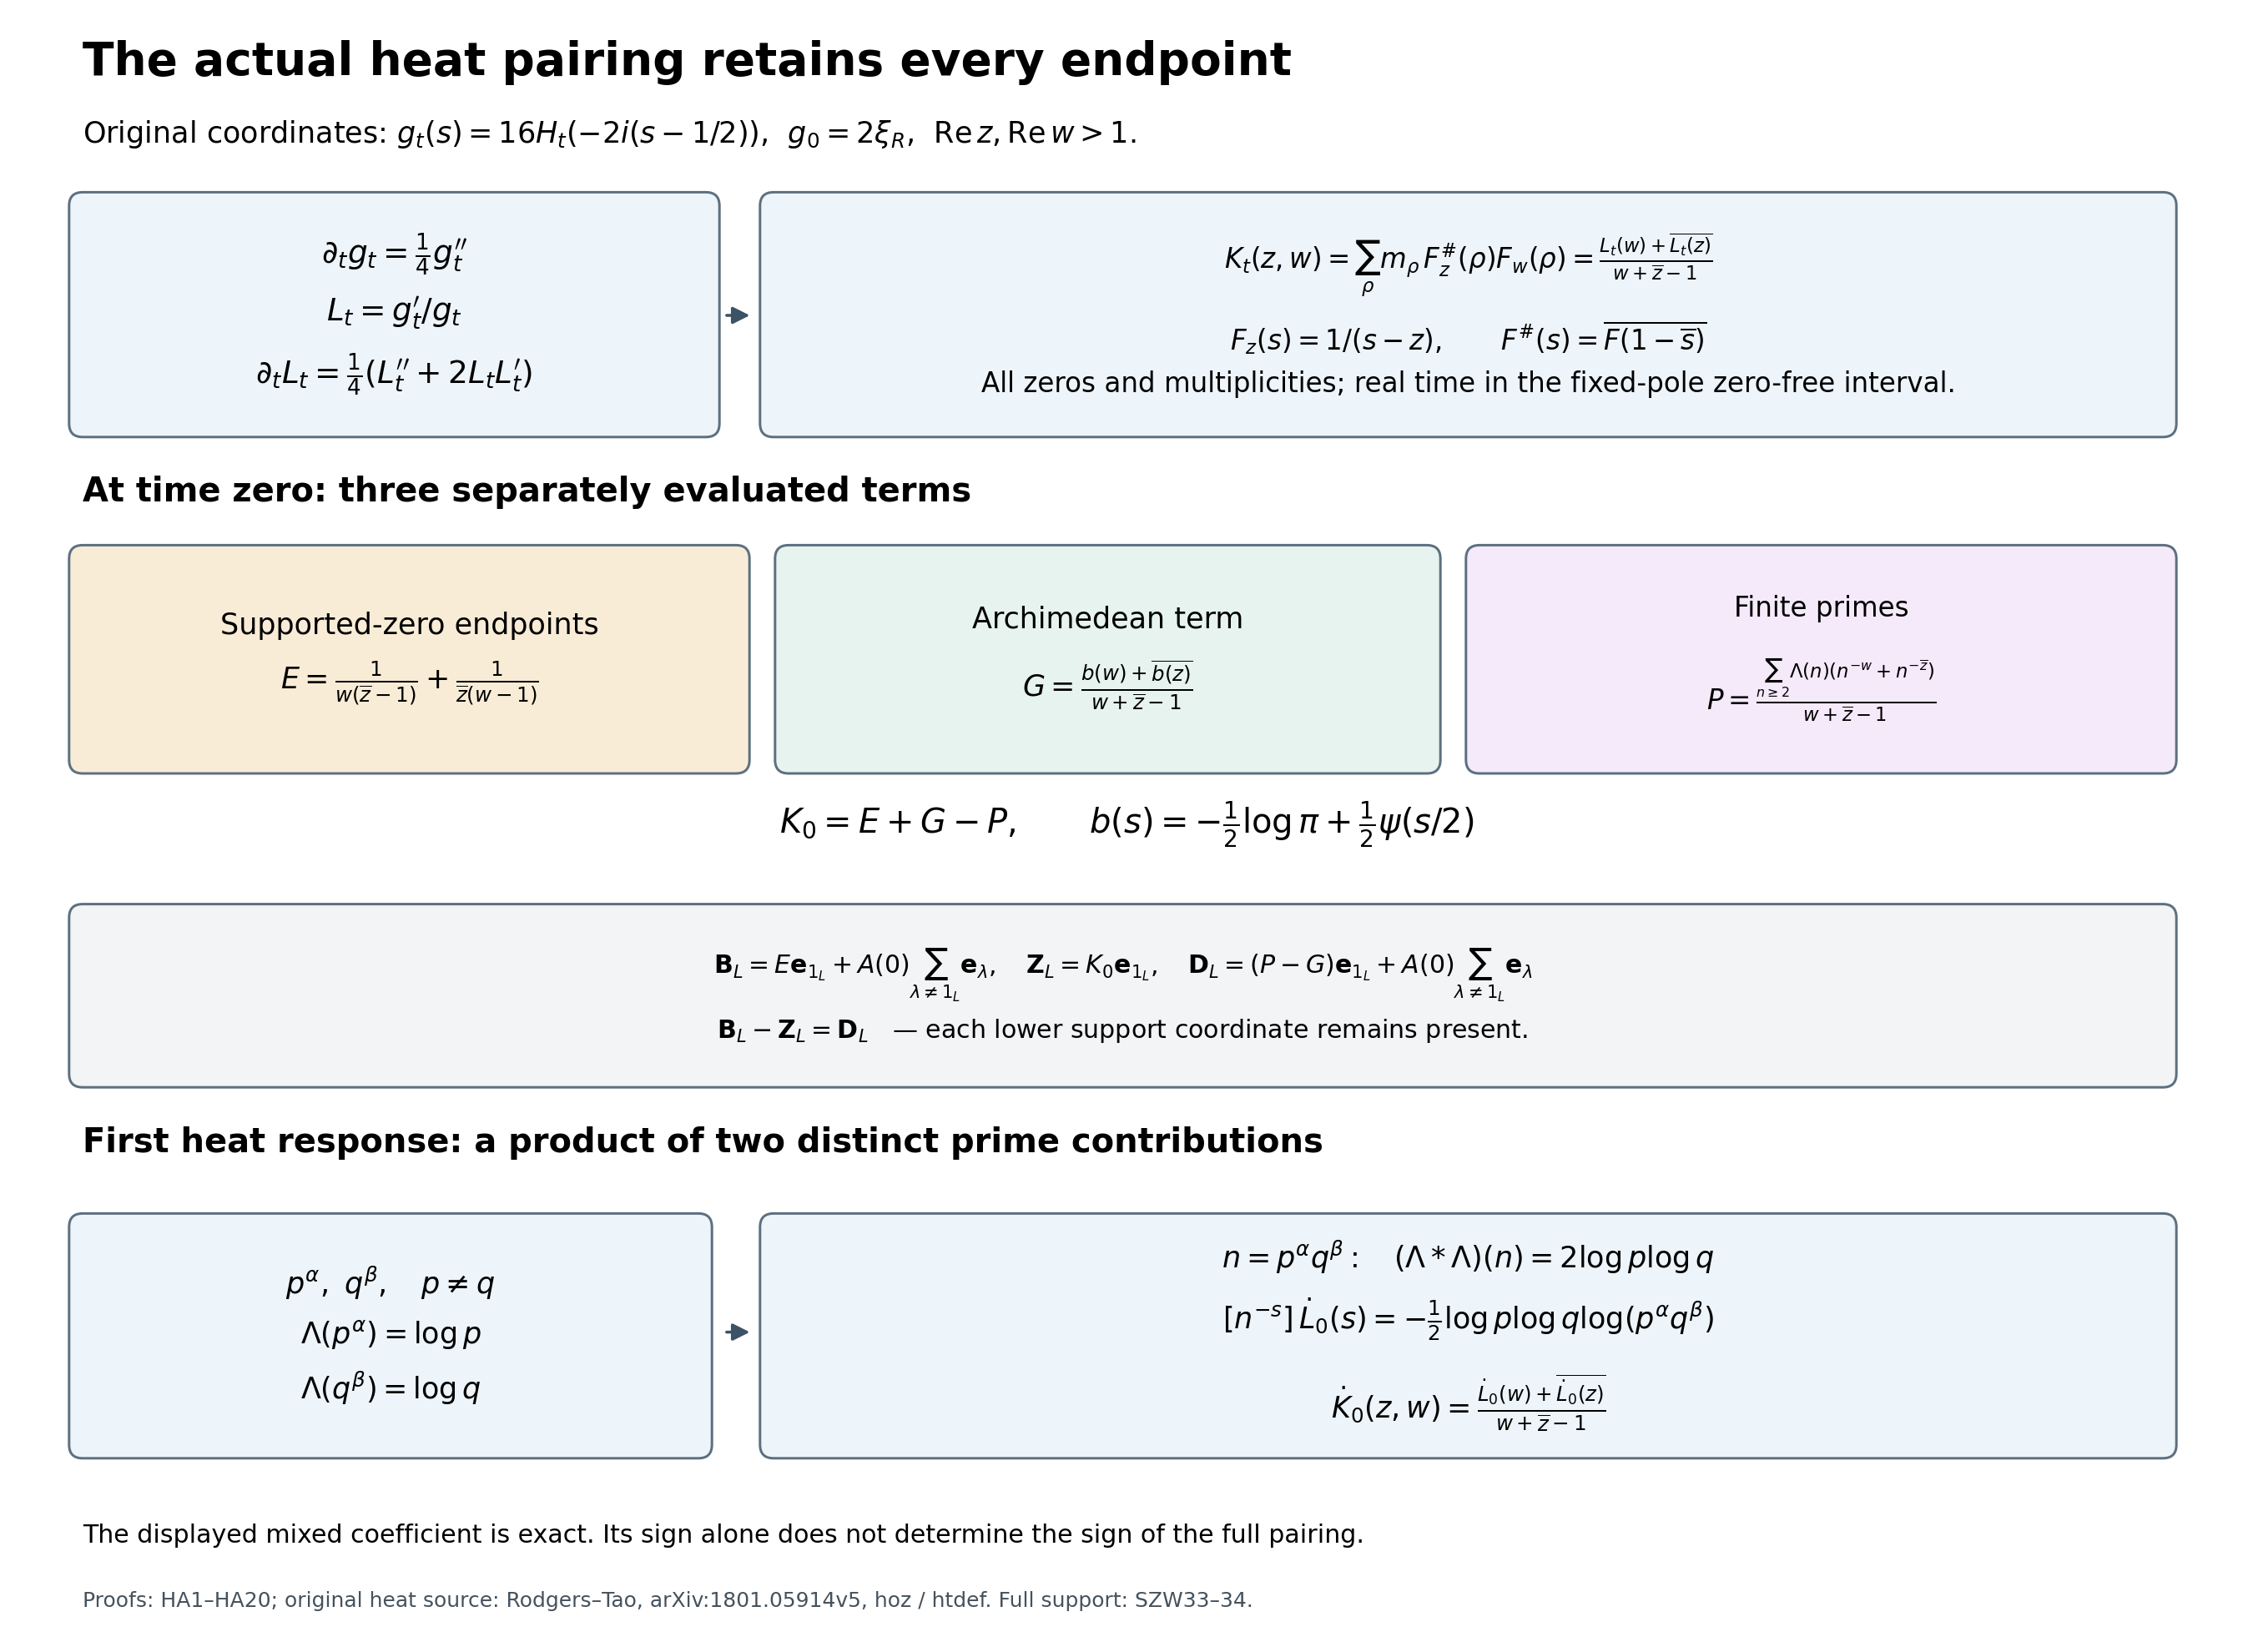
\includegraphics[keepaspectratio,alt={The actual heat coordinates, complete supported arithmetic identity, and first mixed-prime coefficient. Every constant and support coordinate is retained; full proofs HA1--HA20. Here A=F\_z sharp times F\_w as defined in HA5.}]{heat_cauchy_supported_arithmetic.png}}
\caption{The actual heat coordinates, complete supported arithmetic
identity, and first mixed-prime coefficient. Every constant and support
coordinate is retained; full proofs HA1--HA20. Here A=F\_z sharp times
F\_w as defined in HA5.}
\end{figure}

\begin{figure}
\centering
\pandocbounded{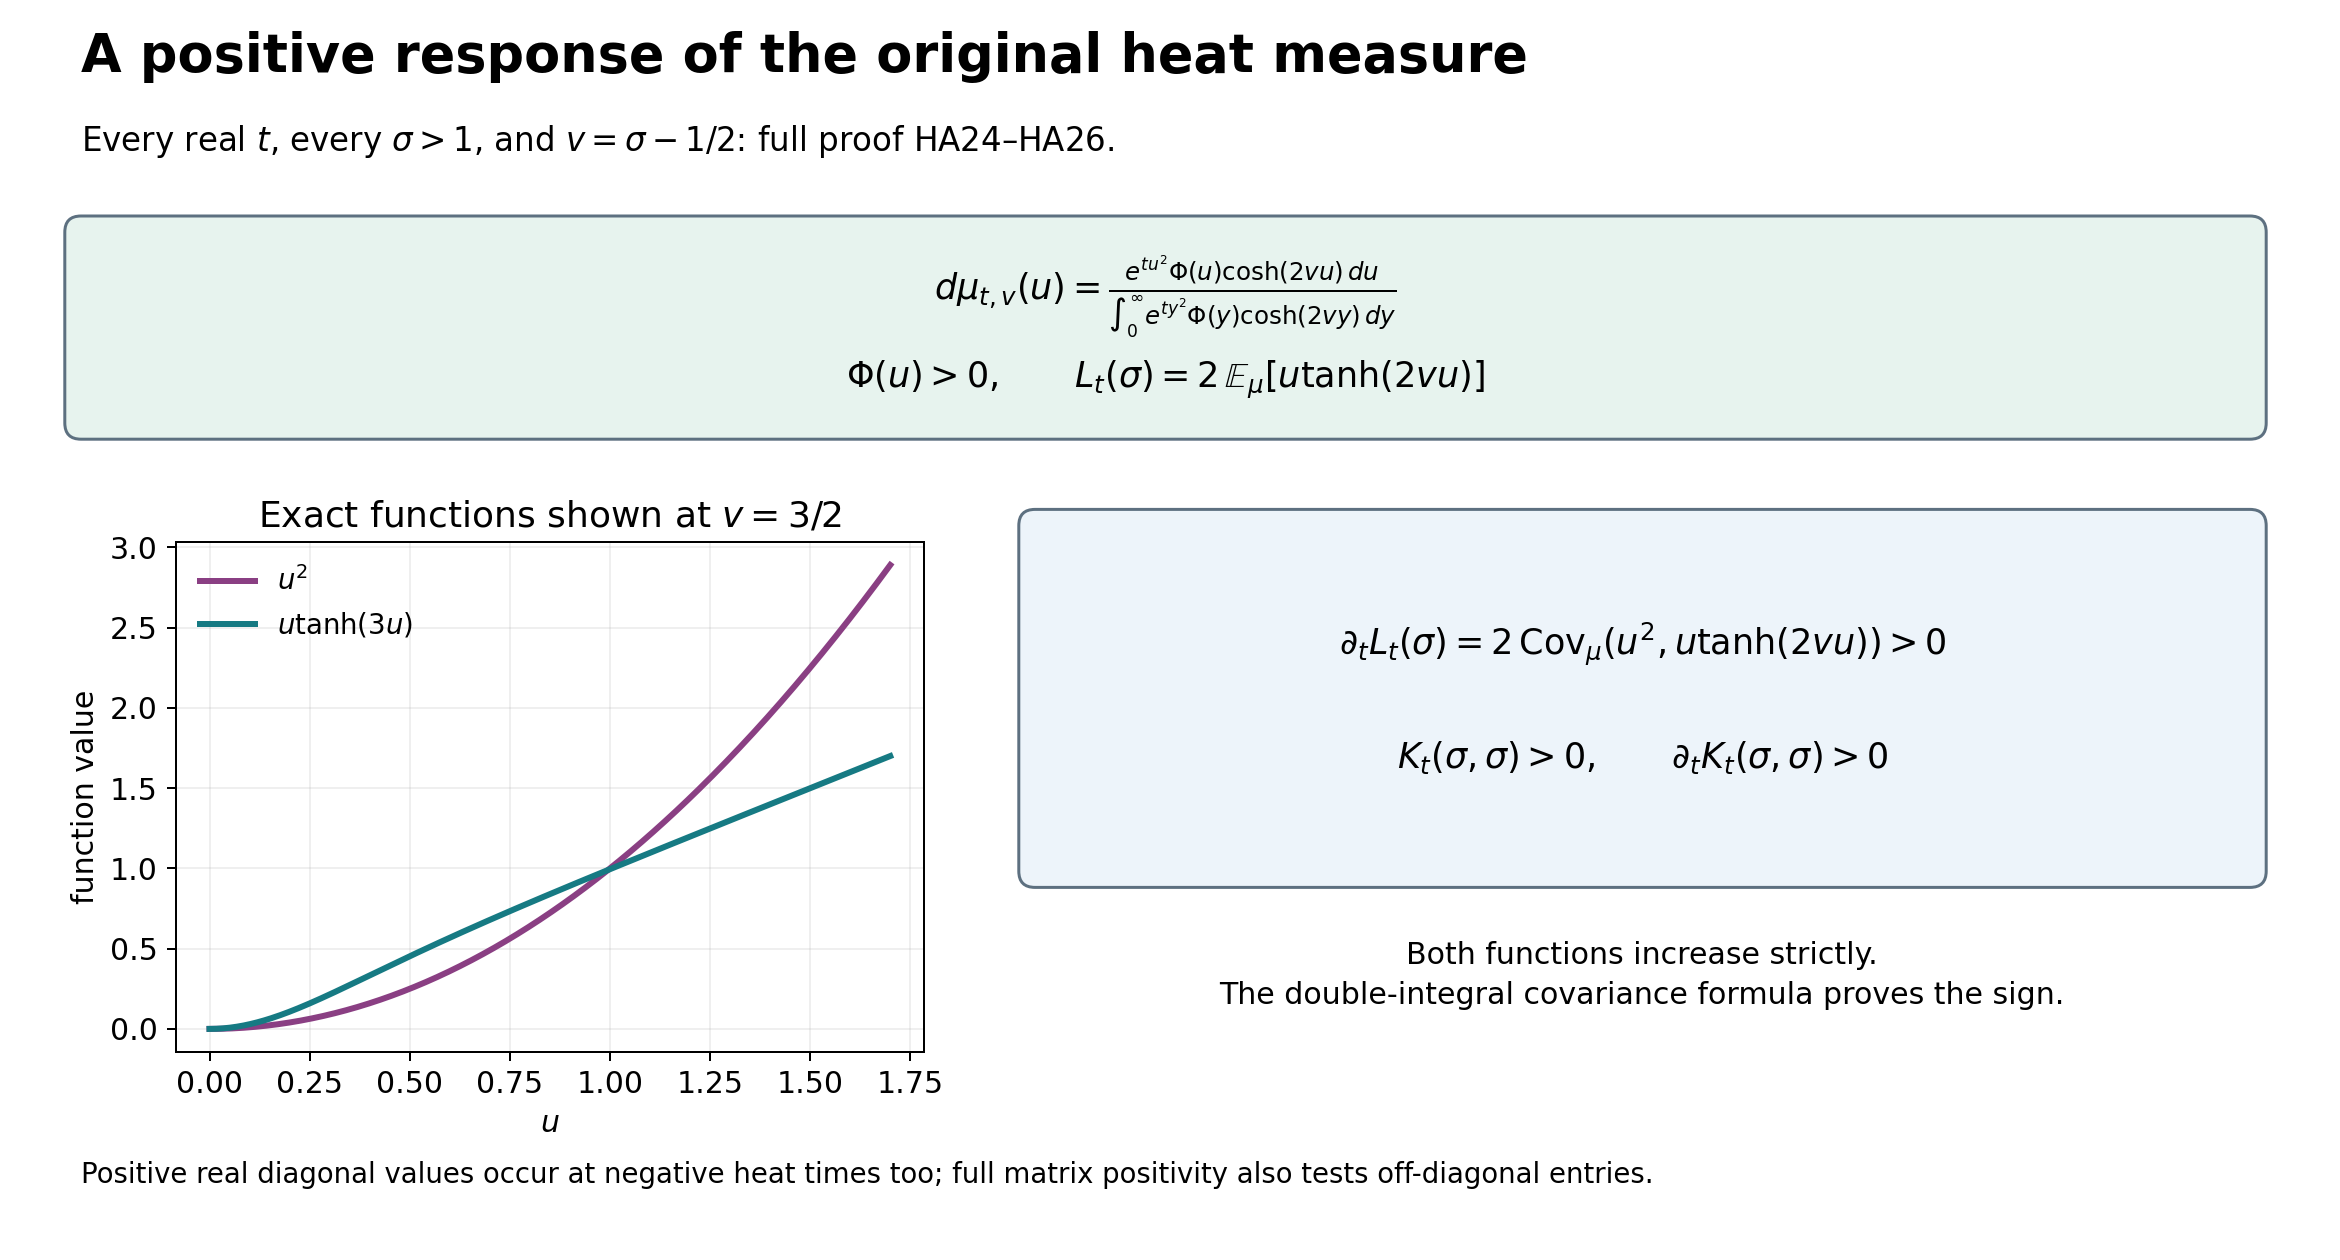
\includegraphics[keepaspectratio,alt={The original positive heat measure and the strict covariance calculation. The two plotted functions are shown at the stated value v=3/2; the theorem and exact integral hold for every v=sigma−1/2 with sigma greater than one. Full proof HA24--HA26.}]{heat_real_diagonal_covariance.png}}
\caption{The original positive heat measure and the strict covariance
calculation. The two plotted functions are shown at the stated value
v=3/2; the theorem and exact integral hold for every v=sigma−1/2 with
sigma greater than one. Full proof HA24--HA26.}
\end{figure}

\subsection{Exact full-form
continuation}\label{exact-full-form-continuation-2}

The \href{CAUCHY_REFLECTION_INDEX_DERIVATION.md}{reflection-index
theorem, NI1--32}, calculates the signed index of every complete Cauchy
coefficient tail. The
\href{FINITE_JET_COMPLEMENT_AND_HEAT_TRUNCATION.md}{finite-jet and
endpoint proof, FJ1--29}, preserves the exact finite jets while proving
density on the remaining zeros, derives the full exterior index and
tail, and calculates the second and third actual heat coefficients. All
supported endpoints remain explicit. These results identify the
remaining sign problem without asserting its resolution.

\subsection{One fixed primitive test and the entire prime
window}\label{one-fixed-primitive-test-and-the-entire-prime-window-1}

The \href{PRIME_PROJECTOR_MOBIUS_DERIVATION.md}{prime-operator
calculation}, PM1--41, proves both distinct Fourier support corrections
and their exact map into the full Weil formula. The
\href{PRIMITIVE_SHORT_SUPPORT_DERIVATION.md}{local estimate}, PS1--21,
gives a positive translation-difference remainder. The
\href{UNIVERSAL_PRIMITIVE_TRANSLATION_CRITERION.md}{fixed-test proof},
UP1--35, constructs one compact test whose transform is nonzero at every
possible off-critical zero. The
\href{PRIMITIVE_PRIME_WINDOW_DERIVATION.md}{complete arithmetic
calculation}, PW1--22, expresses its entire translated correlation
through a fixed-width prime window and an explicit archimedean
remainder. Its boundedness is equivalent to RH; that bound remains
unresolved. All boundary coordinates and supported-zero labels remain
explicit.

\subsection{Actual positive-real-time
continuation}\label{actual-positive-real-time-continuation-1}

The complete \href{REAL_TIME_HEAT_TRACE_DERIVATION.md}{real-time proof},
RT1--30, strengthens the compact-test variation in this edition: the
whole zero trace is smooth for the original real heat time t at least
zero, with actual right derivatives at zero. RT16 identifies its first
derivative with the full causal arithmetic distribution, and RT20--27
constructs every higher meromorphic derivative receiver. The contact
comparison retains the unit and inter-zero terms. These results do not
assert a common zero strip for negative or complex time and do not prove
the remaining RH inequality. All original supported carriers remain
present.

\clearpage

\section{Every time derivative of the actual heat logarithmic
derivative}\label{every-time-derivative-of-the-actual-heat-logarithmic-derivative}

\textbf{Original-zeta receiving calculation.} The working meromorphic
function is the original Riemann zeta, with its full Gamma/endpoints
multiplier and its full trivial-zero and pole divisor retained.
\href{FAITHFUL_THETA_COMPLETION_RETURN.md}{TF1--42} proves the original
labelled theta inverse and the actual heat-image defect.
\href{FAITHFUL_UNCOMPLETED_ZETA_HEAT.md}{UZ1--53} proves every
exceptional-point fibre, jet, original-zeta heat term and reflection
orientation.
\href{ORIGINAL_ZETA_COMPACT_WEIL_RECONSTRUCTION.md}{OZC1--48} rederives
the compact contour and interval operator directly from zeta, including
the left-cutoff Gamma boundary, and specifies exactly which compensated
pairing the bounds concern.
\href{ORIGINAL_ZETA_HEAT_CONTACT_RECONSTRUCTION.md}{OZH1--49} rederives
the actual meromorphic heat, rational signed trace, compact-test domain,
contact drift and full causal arithmetic variation. The raw full divisor
and the compensated Weil receiver are linked by their displayed
correction, not identified. In particular the fixed-test trivial-zero
sum converges exactly at translations at least 1/32 and equals the
earlier R term; at zero translation it requires the proved cutoff
compensation. \href{ORIGINAL_ZETA_CAUCHY_RECONSTRUCTION.md}{OZK1--38}
reconstructs the original signed Cauchy trace, its full Gamma
correction, resonant finite parts, every finite matrix and its index,
and the complete local heat jets. Its invertible map retains the raw
trace and correction separately. These complete receiving proofs govern
the interpretation of the retained auxiliary calculations below.

The original family is \(g_t(s)=16H_t(-2i(s-1/2))\), with
\(\partial_tg_t=\tfrac14\partial_s^2g_t\). Its coordinate, analytic
convergence, and complete supported arithmetic receiver are proved in
\href{HEAT_CAUCHY_ARITHMETIC_DERIVATION.md}{HA1--HA26}. This note
computes its time derivatives without replacing any Gamma or endpoint
coefficient by a constant.

\subsection{1. The exact differential-polynomial
recurrence}\label{the-exact-differential-polynomial-recurrence}

Let \(\mathscr P=\mathbb Q[X_0,X_1,\ldots]\) be the polynomial ring in
countably many variables; each polynomial uses only finitely many of
them. Define commuting spatial and evolutionary derivations by \[
D X_j=X_{j+1},\qquad
V X_j=D^j\!\left(\frac{X_2+2X_0X_1}{4}\right).
\tag{HM1}
\] Both extend uniquely by the Leibniz rule and linearity. Their
commutator is a derivation and is zero on every generator, because
\(DVX_j=VDX_j\); therefore \(DV=VD\). Put \[
B_0=X_0,\qquad B_{k+1}=VB_k
=\sum_{j\ge0}\frac{\partial B_k}{\partial X_j}
D^j\!\left(\frac{X_2+2X_0X_1}{4}\right).
\tag{HM2}
\] The sum is finite for each \(k\). Where \(g_t\ne0\), set
\(L_t=g_t'/g_t\). HA3 and the chain rule prove by induction the exact
identity \[
\partial_t^kL_t(s)=B_k(L_t(s),L_t'(s),L_t''(s),\ldots).
\tag{HM3}
\] These are derivatives, not coefficients of a Taylor series; the
Taylor coefficient is \(B_k/k!\). Each formula is valid as a meromorphic
identity in \(s\) and locally holomorphically in \(t\) away from its
zeros.

Give every \(X_j\) polynomial degree one. The derivation \(D\) preserves
this degree. Split \(V=V_1+V_2\), where \[
V_1X_j=\tfrac14X_{j+2},\qquad
V_2X_j=\tfrac12D^j(X_0X_1).
\tag{HM4}
\] Thus \(V_1\) preserves homogeneous degree and \(V_2\) increases it by
one. In particular \(\deg B_k\le k+1\). Its homogeneous component of
degree \(k+1\) is exactly \[
\boxed{B_k^{[k+1]}=\frac1{2^k(k+1)}D^k(X_0^{k+1}).}
\tag{HM5}
\] Here is the full induction. At \(k=0\) the formula gives \(X_0\). As
with \(V\), the derivation \(V_2\) commutes with \(D\). The only term
capable of producing degree \(k+2\) in \(B_{k+1}\) is
\(V_2B_k^{[k+1]}\). Applying the induction hypothesis gives \[
\begin{aligned}
V_2B_k^{[k+1]}
&=\frac1{2^k(k+1)}D^k\!\left((k+1)X_0^k\frac{X_0X_1}{2}\right)\\
&=\frac1{2^{k+1}(k+2)}D^{k+1}(X_0^{k+2}),
\end{aligned}\tag{HM6}
\] as required. This polynomial is nonzero; its monomial \(X_0^kX_k\)
has a positive coefficient. Hence \(\deg B_k=k+1\), not only the upper
bound.

For clarity the first two nonconstant polynomials are \[
\begin{aligned}
B_1&=\frac14(X_2+2X_0X_1),\\
B_2&=\frac1{16}\left(X_4+8X_1X_2+4X_0X_3
+8X_0X_1^2+4X_0^2X_2\right).
\end{aligned}\tag{HM7}
\] They follow by one and two direct applications of (HM2). In
particular the coefficient of \(X_1X_2\) is eight; no factor is absorbed
into a change of heat time.

\subsection{2. The specified arithmetic
expansion}\label{the-specified-arithmetic-expansion}

On \(\Re s>1\), retain the exact split \[
\begin{aligned}
L_0(s)&=a(s)+r(s),\\
a(s)&=\frac1s+\frac1{s-1}-\frac12\log\pi+\frac12\psi(s/2),\\
r(s)&=-\sum_{n\ge2}\Lambda(n)n^{-s}.
\end{aligned}\tag{HM8}
\] The coefficient functions \(a,a',\ldots\) are retained. The expansion
meant here has an explicit rule: in \(B_k\) substitute
\(X_j=a^{(j)}+r^{(j)}\), expand each monomial, and multiply the
absolutely convergent Dirichlet series in the \(r^{(j)}\) factors by
ordered Dirichlet convolution. A term with no \(r\) factor remains its
original coefficient function. This is a specified representation; no
uniqueness claim is made for expansions with arbitrary \(s\)-dependent
coefficients.

Every factor \(r^{(j)}\) has series \[
r^{(j)}(s)=-\sum_{n\ge2}\Lambda(n)(-\log n)^j n^{-s}.
\tag{HM9}
\] Each derivative converges absolutely and locally uniformly on the
half-plane. Finite products do too, because their absolute multiple sums
are bounded by the product of the convergent single sums. Thus the
expansion rule and every spatial derivative used below are justified
there.

Since each nonzero coefficient of one factor is supported on prime
powers, a product of \(j\) such factors is supported on integers with at
most \(j\) distinct prime factors. By (HM4)--(HM5), the arithmetic
coefficient at an integer with more than \(k+1\) distinct prime factors
is zero in this specified expansion of \(\partial_t^kL_t|_0\).

For an integer with exactly \(k+1\) distinct prime factors, write \[
n=\prod_{i=1}^{k+1}p_i^{\alpha_i},\qquad
p_i\ne p_j\ (i\ne j),\quad\alpha_i\ge1.
\tag{HM10}
\] Only the homogeneous component of degree \(k+1\), with every factor
chosen from \(r\), can contribute. Any \(a\) factor would reduce the
number of available prime-power factors. Therefore its coefficient is
the coefficient in \[
\frac1{2^k(k+1)}\partial_s^k(r(s)^{k+1}).
\tag{HM11}
\] To compute it, each of the \(k+1\) ordered factors must receive one
of the distinct prime powers in (HM10). There are exactly \((k+1)!\)
such assignments. No exponent can split between two factors, because
that would leave a different prime without a factor. Hence the
coefficient of \(r^{k+1}\) at \(n\) is
\((-1)^{k+1}(k+1)!\prod_i\log p_i\). Applying \(\partial_s^k\)
multiplies it by \((-\log n)^k\). The two signs combine to minus,
proving \[
\boxed{[n^{-s}]\left.\partial_t^kL_t(s)\right|_0
=-\frac{k!}{2^k}(\log n)^k\prod_{i=1}^{k+1}\log p_i.}
\tag{HM12}
\] The bracket refers exactly to the expansion rule after (HM8). The
displayed coefficient has no remaining \(a(s)\) dependence. At lower
distinct-prime counts all coefficient functions prescribed by that rule
remain present.

For \(k=0\), (HM12) is the original coefficient \(-\log p\) at
\(p^\alpha\). For \(k=1\) it is
\(-\tfrac12\log p\log q\log(p^\alpha q^\beta)\), agreeing with HA19. For
\(k=2\) it is \(-\tfrac12(\log n)^2\log p\log q\log r\) at three
distinct prime factors. Formula (HM12) concerns a time derivative;
dividing by \(k!\) gives the coefficient in the actual Taylor series in
time.

\subsection{3. The global supported
receiver}\label{the-global-supported-receiver}

For the original Cauchy tests at \(z,w\) in \(\Re s>1\), the exact
global family of \href{HEAT_CAUCHY_ARITHMETIC_DERIVATION.md}{HA5--HA20}
gives, for every \(k\), \[
\left.\partial_t^kK_t(z,w)\right|_0
=\frac{B_k(L_0,L_0',\ldots)(w)
+\overline{B_k(L_0,L_0',\ldots)(z)}}{w+\bar z-1}.
\tag{HM13}
\] Indeed the finite-pole formula is holomorphic on a time disc for this
finite test set, so it may be differentiated any finite number of times;
(HM3) supplies the derivatives. All coefficients of \(B_k\) are real.
The fixed supported boundary and every lower coordinate have zero time
derivative for \(k\ge1\). The corresponding geometric-divisor response
is the negative of (HM13) in the top coordinate, with no suppressed
lower distribution, by HA20.

This constructs actual arithmetic mixed-prime data at every
infinitesimal order. The negative coefficient in (HM12) is not the value
of a quadratic form: the matrix denominator, conjugate counterpart,
remaining coefficients, Gamma factors and endpoints in (HM13) are still
present. The complete sign question is the
\href{CAUCHY_WEIL_POSITIVITY_CRITERION.md}{Cauchy--Weil matrix
criterion}.

\subsection{Verification and sources}\label{verification-and-sources}

The accompanying \texttt{check\_\allowbreak{}heat\_\allowbreak{}mixed\_\allowbreak{}prime\_\allowbreak{}recurrence.\allowbreak{}py}
computes the entire recurrence through order six in the differential
polynomial ring, checks its exact degree, and compares every
highest-degree component with (HM5). Its monomial counts are 1, 2, 5,
11, 23, 44 and 82. These finite checks supplement the all-order proof
(HM4)--(HM6).

The human heat source remains Brad Rodgers and Terence Tao,
\href{https://arxiv.org/src/1801.05914v5}{arXiv:1801.05914v5, original
author TeX}, equations \texttt{hoz}, \texttt{htdef} and the subsequent
heat equation. The full supported explicit formula is
\href{https://github.com/KokunoYumeto/zeta-function-research-reader/blob/3c022a0adde0a6aa3d8fc8e43ef42795d88e44b0/workbenches/splitzero-tandem/branches/tau-zero-prime-positivity/SUPPORTED_ZERO_PRIME_WEIL_DERIVATION.md}{SZW19--SZW38},
with its original human sources retained. The logarithmic-derivative
equation is the classical Burgers transformation of the heat equation;
its exact normalization and every recurrence used here have been proved
above. No novelty claim for that transformation is made.

\subsection{Actual positive-real-time
continuation}\label{actual-positive-real-time-continuation-2}

The complete \href{REAL_TIME_HEAT_TRACE_DERIVATION.md}{real-time proof},
RT1--30, strengthens the compact-test variation in this edition: the
whole zero trace is smooth for the original real heat time t at least
zero, with actual right derivatives at zero. RT16 identifies its first
derivative with the full causal arithmetic distribution, and RT20--27
constructs every higher meromorphic derivative receiver. The contact
comparison retains the unit and inter-zero terms. These results do not
assert a common zero strip for negative or complex time and do not prove
the remaining RH inequality. All original supported carriers remain
present.

\clearpage

\section{The complete Cauchy--Weil matrix
criterion}\label{the-complete-cauchyweil-matrix-criterion}

\textbf{Original-zeta receiving calculation.} The working meromorphic
function is the original Riemann zeta, with its full Gamma/endpoints
multiplier and its full trivial-zero and pole divisor retained.
\href{FAITHFUL_THETA_COMPLETION_RETURN.md}{TF1--42} proves the original
labelled theta inverse and the actual heat-image defect.
\href{FAITHFUL_UNCOMPLETED_ZETA_HEAT.md}{UZ1--53} proves every
exceptional-point fibre, jet, original-zeta heat term and reflection
orientation.
\href{ORIGINAL_ZETA_COMPACT_WEIL_RECONSTRUCTION.md}{OZC1--48} rederives
the compact contour and interval operator directly from zeta, including
the left-cutoff Gamma boundary, and specifies exactly which compensated
pairing the bounds concern.
\href{ORIGINAL_ZETA_HEAT_CONTACT_RECONSTRUCTION.md}{OZH1--49} rederives
the actual meromorphic heat, rational signed trace, compact-test domain,
contact drift and full causal arithmetic variation. The raw full divisor
and the compensated Weil receiver are linked by their displayed
correction, not identified. In particular the fixed-test trivial-zero
sum converges exactly at translations at least 1/32 and equals the
earlier R term; at zero translation it requires the proved cutoff
compensation. \href{ORIGINAL_ZETA_CAUCHY_RECONSTRUCTION.md}{OZK1--38}
reconstructs the original signed Cauchy trace, its full Gamma
correction, resonant finite parts, every finite matrix and its index,
and the complete local heat jets. Its invertible map retains the raw
trace and correction separately. These complete receiving proofs govern
the interpretation of the retained auxiliary calculations below.

This note proves an equivalence with the classical Riemann hypothesis.
It does not assume or establish positivity of the matrices occurring in
that equivalence. The full supported-zero arithmetic evaluation of those
matrices is \href{HEAT_CAUCHY_ARITHMETIC_DERIVATION.md}{HA10--HA20};
every endpoint and lower support coordinate remains there.

\subsection{1. The original kernel and zero
sum}\label{the-original-kernel-and-zero-sum}

Put \(g=2\xi_R\), \(L=g'/g\), and \(\mathcal U=\{z:\Re z>1\}\). Define
\[
K(z,w)=\frac{L(w)+\overline{L(z)}}{w+\bar z-1},\qquad z,w\in\mathcal U.
\tag{CK1}
\] The unconditional Euler product and functional equation imply that
\(g\) is nonzero on \(\mathcal U\), so this definition requires no RH
assumption. The exact global trace identity AG10--AG11 is \[
K(z,w)=\sum_\rho m_\rho
\overline{F_z(\rho^\#)}F_w(\rho),\qquad
F_z(s)=\frac1{s-z},\quad\rho^\#=1-\bar\rho.
\tag{CK2}
\] The sum converges absolutely and keeps all multiplicities. The
reflection and Hadamard proof, with the zero count, is given in
\href{ACTUAL_HEAT_ZERO_DISTRIBUTION_VARIATION.md}{AG1--AG11}.

A kernel is positive semidefinite on a set when, for every integer
\(n\ge1\), every finite tuple of points in that set, and every
\(c\in\mathbb C^n\), its quadratic sum
\(\sum_{i,j}\bar c_iK(z_i,z_j)c_j\) is nonnegative. Under RH each
\(\rho^\#=\rho\), so (CK2) gives \[
\sum_{i,j}\bar c_iK(z_i,z_j)c_j
=\sum_\rho m_\rho\left|\sum_j c_jF_{z_j}(\rho)\right|^2\ge0.
\tag{CK3}
\] This proves one direction. The converse is proved completely below,
including the extension of a kernel known only on the observed
subdomain.

\subsection{2. A self-contained Schur extension from a positive
kernel}\label{a-self-contained-schur-extension-from-a-positive-kernel}

The positive-kernel Hilbert construction and the transfer-function
realization used in this section are classical. A primary-source
treatment is Joseph A. Ball, Animikh Biswas, Quanlei Fang and Sanne ter
Horst, \emph{Multivariable generalizations of the Schur class: positive
kernel characterization and transfer function realization},
\href{https://arxiv.org/abs/0705.2042v3}{arXiv:0705.2042v3}, §1, Theorem
1.1(2)--(3) and Proposition 1.2. Their proof discussion of Theorem 1.1,
(2) ⇒ (3), identifies the equal-Gram construction as the standard
lurking-isometry argument. The source orders its Hilbert sum as
\(\mathcal H\oplus\mathbb C\), whereas CK5--CK7 use
\(\mathbb C\oplus\mathcal H\). The unitary swap
\(J(\alpha,h)=(h,\alpha)\) sends
\(V=\left(\begin{smallmatrix}a&b\\c&d\end{smallmatrix}\right)\) to
\(JVJ^{-1}=\left(\begin{smallmatrix}d&c\\b&a\end{smallmatrix}\right)\).
Thus the source's blocks are \((A,B,C,D)=(d,c,b,a)\), and its transfer
formula \(D+zC(I-zA)^{-1}B\) is exactly CK7. In the scalar case its
kernel \(K_f(y,x)\) is CK4's \(S(x,y)\), retaining the
conjugate-linear-first convention. The cited theorem is stated on the
full disc; the arbitrary-subset extension needed here is proved directly
below, rather than asserted to be an additional theorem read in that
source.

Let \(E\) be any nonempty subset of the unit disc, and let
\(f:E\to\mathbb C\) satisfy positivity of \[
S(x,y)=\frac{1-\overline{f(x)}f(y)}{1-\bar x y}.
\tag{CK4}
\] We construct a holomorphic function \(\widetilde f\) on the whole
unit disc, of modulus at most one, agreeing with \(f\) on \(E\). First
construct a Hilbert space \(\mathcal H\) from formal vectors \(v_x\),
setting \(\langle v_x,v_y\rangle=S(x,y)\), with the inner product
conjugate-linear in its first variable. On finite linear combinations
this is a nonnegative sesquilinear form. Cauchy--Schwarz for such a form
follows from positivity of the quadratic polynomial in a complex scalar;
consequently its zero-length vectors form its radical. Quotient by this
radical and complete to obtain \(\mathcal H\).

The identity in (CK4) gives equal Gram matrices for the following two
families in \(\mathbb C\oplus\mathcal H\): \[
\begin{pmatrix}1\\xv_x\end{pmatrix}
\longmapsto
\begin{pmatrix}f(x)\\v_x\end{pmatrix},
\qquad
1+\bar x yS(x,y)=\overline{f(x)}f(y)+S(x,y).
\tag{CK5}
\] The rule therefore defines a well-defined isometry on their algebraic
span and extends to its closure \(\mathcal M\). Extend it to a
contraction \(V\) on \(\mathbb C\oplus\mathcal H\) by setting it equal
to zero on \(\mathcal M^\perp\). Write its bounded blocks as \[
V=\begin{pmatrix}a&b\\c&d\end{pmatrix},\qquad \|V\|\le1.
\tag{CK6}
\] Here \(a\in\mathbb C\), \(b:\mathcal H\to\mathbb C\),
\(c:\mathbb C\to\mathcal H\) is identified with \(c(1)\), and
\(d:\mathcal H\to\mathcal H\). Equation (CK5) says \(a+xbv_x=f(x)\) and
\(c+xdv_x=v_x\). Since \(\|d\|\le1\), the Neumann series makes \(I-zd\)
invertible for every \(|z|<1\). Define \[
h(z)=(I-zd)^{-1}c,\qquad
\widetilde f(z)=a+zb(I-zd)^{-1}c.
\tag{CK7}
\] The series makes both holomorphic and gives \(h(x)=v_x\),
\(\widetilde f(x)=f(x)\). Moreover
\(V(1,zh(z))=(\widetilde f(z),h(z))\). Contractivity yields \[
|\widetilde f(z)|^2+\|h(z)\|^2
\le1+|z|^2\|h(z)\|^2,
\quad
1-|\widetilde f(z)|^2\ge(1-|z|^2)\|h(z)\|^2\ge0.
\tag{CK8}
\] This proves the required extension without invoking an unproved
interpolation theorem. It is the classical Schur transfer construction,
with its spaces and maps specified here; no novelty claim for the
construction is made.

\subsection{3. Positive Cauchy matrices exclude every zero off the
line}\label{positive-cauchy-matrices-exclude-every-zero-off-the-line}

Write \(v=s-1/2\). The half-plane \(\Re s>1/2\) is carried bijectively
to the unit disc by \[
x=\frac{v-1}{v+1}=\frac{s-3/2}{s+1/2},\qquad
s=\frac12+\frac{1+x}{1-x}.
\tag{CK9}
\] Let \(U\) be any nonempty open subset of \(\mathcal U\) on which
\(K\) is positive semidefinite. Its diagonal gives
\(2\Re L(s)/(2\Re s-1)\ge0\), hence \(\Re L(s)\ge0\) on \(U\). In
particular \(L(s)+1\ne0\). Put \[
f(x)=\frac{L(s)-1}{L(s)+1},\qquad x=x(s),\ s\in U.
\tag{CK10}
\] The exact kernel transformation is \[
\frac{1-\overline{f(x(z))}f(x(w))}{1-\overline{x(z)}x(w)}
=\overline{a(z)}K(z,w)a(w),\quad
a(s)=\frac{s+1/2}{L(s)+1}.
\tag{CK11}
\] Indeed the numerator before division is
\(2(\overline{L(z)}+L(w))/((\overline{L(z)}+1)(L(w)+1))\); the disc
denominator is \(2(w+\bar z-1)/((\bar z+1/2)(w+1/2))\). Their quotient
gives (CK11) exactly. A diagonal congruence preserves kernel positivity.
Section 2 therefore extends \(f\) to a Schur function \(\widetilde f\)
on the whole unit disc.

The extended function cannot take the value 1 inside the disc. Otherwise
the maximum modulus principle makes it identically 1, contradicting
(CK10) at any point of \(U\). Thus \[
\widetilde L(s)=\frac{1+\widetilde f(x(s))}{1-\widetilde f(x(s))}
\tag{CK12}
\] is holomorphic on \(\Re s>1/2\) and equals the original \(L\) on
\(U\). The holomorphic function \(g'-\widetilde Lg\) on this connected
half-plane vanishes on \(U\), so the identity theorem makes it zero
throughout. If \(g\) had a zero \(\rho\) of positive multiplicity \(m\)
there, then \(g'\) would have order \(m-1\) at \(\rho\), while
\(\widetilde Lg\) has order at least \(m\). This contradicts the
identity. Hence \(g\) has no zeros in \(\Re s>1/2\). The functional
equation \(g(1-s)=g(s)\) excludes zeros in \(\Re s<1/2\) as well. Its
zeros are exactly the nontrivial zeta zeros, proving RH.

Together with (CK3) this proves the exact equivalence \[
\boxed{\begin{aligned}
\mathrm{RH}&\Longleftrightarrow K\text{ is positive semidefinite on }\mathcal U\\
&\Longleftrightarrow K\text{ is positive semidefinite on }U.
\end{aligned}}
\tag{CK13}
\] The last phrase means that for each fixed such \(U\), its complete
positivity condition is equivalent to RH. It does not replace all finite
matrices by a single diagonal inequality.

\subsection{4. One real point, with every Taylor coefficient
retained}\label{one-real-point-with-every-taylor-coefficient-retained}

Fix a real \(\sigma>1\), write \(d=2\sigma-1\), and set
\(\ell_n=L^{(n)}(\sigma)/n!\). All \(\ell_n\) are real. Define the
infinite Hermitian coefficient matrix \[
C_{jk}=[X^jY^k]\frac{L(\sigma+X)+L(\sigma+Y)}{d+X+Y},\qquad j,k\ge0.
\tag{CK14}
\] The bracket denotes the convergent Taylor expansion near \(X=Y=0\),
not a truncation of the underlying function. Expanding the denominator
geometrically gives the explicit coefficients \[
\begin{aligned}
C_{jk}={}&\sum_{n=0}^j
\ell_n\frac{(-1)^{j+k-n}\binom{j+k-n}{k}}{d^{j+k-n+1}}\\
&+\sum_{n=0}^k
\ell_n\frac{(-1)^{j+k-n}\binom{j+k-n}{j}}{d^{j+k-n+1}}.
\end{aligned}\tag{CK15}
\] In particular, \(\ell_0\) occurs twice, as it must in the numerator
of (CK14).

The entries are exactly the original rational-jet pairings \[
C_{jk}=Z_0\!\left((Q_j)^\#Q_k\right),\qquad
Q_j(s)=\frac1{(s-\sigma)^{j+1}}.
\tag{CK16}
\] To verify this, \(F_{\sigma+Y}(s)=\sum_{k\ge0}Y^k/(s-\sigma)^{k+1}\)
on any sufficiently small parameter disc at each zero. The analogous
reflected expansion uses \(X\). Derivatives may be taken in (CK2)
locally: its large-zero tail, and every parameter derivative of that
tail, are uniformly summable by the \(O(|\rho|^{-2})\) bound and the
fixed distance of the poles from the critical strip. The finitely many
remaining terms are analytic. Coefficient comparison now gives (CK16),
with no missing factorial.

We prove the complete single-point criterion: \[
\boxed{\mathrm{RH}\quad\Longleftrightarrow\quad
(C_{jk})_{0\le j,k\le N}\succeq0\text{ for every integer }N\ge0.}
\tag{CK17}
\] Under RH, (CK16) is a positive Gram matrix by (CK3). Conversely
suppose every indicated finite section is positive. Choose a small disc
\(|z-\sigma|<r\) contained in \(\mathcal U\), on whose product the
double Taylor series in (CK14) converges absolutely. For finitely many
points \(z_i\) in a smaller such disc and coefficients \(b_i\), put
\(v_j=\sum_i b_i(z_i-\sigma)^j\). Positivity of the finite sections
gives \(\sum_{j,k=0}^N\bar v_jC_{jk}v_k\ge0\). Absolute convergence
allows \(N\to\infty\), yielding \(\sum_{i,l}\bar b_iK(z_i,z_l)b_l\ge0\).
Thus \(K\) is positive on a nonempty open disc, and (CK13) proves RH.
This keeps the entire coefficient tower; no finite \(N\) is claimed
sufficient.

The first two-by-two section retains a useful exact determinant: \[
\begin{pmatrix}C_{00}&C_{01}\\C_{10}&C_{11}\end{pmatrix}
=\begin{pmatrix}
2\ell_0/d&\ell_1/d-2\ell_0/d^2\\
\ell_1/d-2\ell_0/d^2&-2\ell_1/d^2+4\ell_0/d^3
\end{pmatrix},\qquad
\det=\frac{4\ell_0^2-d^2\ell_1^2}{d^4}.
\tag{CK18}
\] This follows by expanding the displayed determinant; no derivative of
order two enters this particular mixed coefficient. Higher sections do
retain higher derivatives through (CK15).

\subsection{5. The actual heat response of the whole coefficient
tower}\label{the-actual-heat-response-of-the-whole-coefficient-tower}

Let \(L_t=g_t'/g_t\) for the original heat family. At the fixed real
\(\sigma>1\), the positive integral makes \(g_t(\sigma)>0\) for every
real time. Define \(C_{jk}(t)\) by the same local Taylor formula as
(CK14). For each fixed time and each finite coefficient set the function
is holomorphic on a time disc; the proof is AG1--AG11. Therefore \[
\left.\partial_t^k C_{ij}(t)\right|_0
=[X^iY^j]\frac{B_k(L_0,L_0',\ldots)(\sigma+X)
+B_k(L_0,L_0',\ldots)(\sigma+Y)}{d+X+Y},
\tag{CK19}
\] where the full recurrence and all mixed-prime coefficients are proved
in \href{HEAT_MIXED_PRIME_RECURRENCE.md}{HM1--HM13}. Equation (CK19) is
the exact map from the arithmetic heat derivative to the complete
positivity tower. The rational tests in (CK16) carry the supported
endpoints and lower fixed coordinates of SZW through AG16; no coordinate
of that identity is removed to define the tower.

HA24--HA26 proves that \(C_{00}(t)>0\) and \(\partial_tC_{00}(t)>0\) for
every real time, including negative times when the actual heat function
has nonreal zeros. Thus positivity of that one entry is a proved
property with a strictly smaller scope than (CK17). The remaining matrix
entries and their exact response (CK19) are concrete mathematical data
retained by the criterion.

\subsection{Method and sources}\label{method-and-sources}

The transfer construction CK4--CK8 is a complete proof of the classical
Schur/Pick extension method used here, rather than an appeal to an
unstated interpolation hypothesis. Jensen, Hadamard and the original
zeta facts required by CK1--CK3 are proved or invoked with verified
hypotheses in AG and SZW. The original human explicit-formula source
remains Alain Connes, \emph{Trace formula in noncommutative geometry and
the zeros of the Riemann zeta function}, Appendix II Theorem 6, as read
and applied in
\href{https://github.com/KokunoYumeto/zeta-function-research-reader/blob/3c022a0adde0a6aa3d8fc8e43ef42795d88e44b0/workbenches/splitzero-tandem/branches/tau-zero-prime-positivity/SUPPORTED_ZERO_PRIME_WEIL_DERIVATION.md}{SZW19--SZW38}.
Rodgers--Tao's original heat coordinates, source locators and archive
are retained in AG and HA. No historical novelty claim for equivalent RH
criteria or classical transfer methods is made. The exact in-programme
contribution is the complete supported arithmetic and original-heat maps
into this specified matrix family.

Ball, Joseph A.; Biswas, Animikh; Fang, Quanlei; ter Horst, Sanne.
\emph{Multivariable generalizations of the Schur class: positive kernel
characterization and transfer function realization}. arXiv:0705.2042v3,
2 November 2007. https://arxiv.org/abs/0705.2042v3 . Original author TeX
inspected, §1, Theorem 1.1, Proposition 1.2 and the proof discussion
through (2) ⇒ (3).

The inspected treatment attributes the scalar positive-kernel
Hilbert-space construction to N. Aronszajn, \emph{Theory of reproducing
kernels}, Transactions of the American Mathematical Society 68 (1950),
337--404. It cites J. A. Ball, \emph{Linear systems, operator model
theory and scattering: multivariable generalizations}, in \emph{Operator
Theory and Its Applications (Winnipeg, MB, 1998)}, Fields Institute
Communications 25, American Mathematical Society, 2000, 151--178, for
the lurking-isometry terminology. These two original works were not
inspected for this repair; this historical attribution is through the
inspected Ball--Biswas--Fang--ter Horst source. No historical novelty
for these classical methods is claimed.

\subsection{One fixed primitive test and the entire prime
window}\label{one-fixed-primitive-test-and-the-entire-prime-window-2}

The \href{PRIME_PROJECTOR_MOBIUS_DERIVATION.md}{prime-operator
calculation}, PM1--41, proves both distinct Fourier support corrections
and their exact map into the full Weil formula. The
\href{PRIMITIVE_SHORT_SUPPORT_DERIVATION.md}{local estimate}, PS1--21,
gives a positive translation-difference remainder. The
\href{UNIVERSAL_PRIMITIVE_TRANSLATION_CRITERION.md}{fixed-test proof},
UP1--35, constructs one compact test whose transform is nonzero at every
possible off-critical zero. The
\href{PRIMITIVE_PRIME_WINDOW_DERIVATION.md}{complete arithmetic
calculation}, PW1--22, expresses its entire translated correlation
through a fixed-width prime window and an explicit archimedean
remainder. Its boundedness is equivalent to RH; that bound remains
unresolved. All boundary coordinates and supported-zero labels remain
explicit.

\subsection{Original-zeta Gaussian and affine receiving
maps}\label{original-zeta-gaussian-and-affine-receiving-maps}

The complete extension OZG1--55 proves that Gaussian convolution of the
test at every positive time makes the original trivial-zero scalar sum
diverge for every real translation. Its admissible replacement retains
each cutoff trace and the Gamma boundary with the identical finite sum
U\_N; OZG20--27 gives both maps and the inverse. The full coefficient
tower, its raw non-Hermitian correction and exact compensated negative
index are OZG28--39. No compact-support prime window is assumed after
smoothing; all prime powers and Gamma terms, with explicit error bounds,
are OZG40--52. This extension acts on the tests while fixing the
original zeta zeros.

The different affine change of the actual original heat family is
OZR1--36. Its multiplier is exp(chi) C(phi)/C, with the full inverse,
exceptional units and local jets. The original generator contains every
q derivative term. The signed divisor comparison is OZR19--24; its
Cauchy logarithmic kernel has an additional growth contribution 2a.
OZR33 proves the exact full negative index after that contribution is
retained. The full support carrier and every lower coordinate are
OZG53--55 and OZR34--36. These are the receiving maps for these
specified extensions; the original preceding test, time and domains
remain those stated in its proof.

\clearpage

\section{The exact reflection index of the global Cauchy--Weil
pairing}\label{the-exact-reflection-index-of-the-global-cauchyweil-pairing}

\textbf{Original-zeta receiving calculation.} The working meromorphic
function is the original Riemann zeta, with its full Gamma/endpoints
multiplier and its full trivial-zero and pole divisor retained.
\href{FAITHFUL_THETA_COMPLETION_RETURN.md}{TF1--42} proves the original
labelled theta inverse and the actual heat-image defect.
\href{FAITHFUL_UNCOMPLETED_ZETA_HEAT.md}{UZ1--53} proves every
exceptional-point fibre, jet, original-zeta heat term and reflection
orientation.
\href{ORIGINAL_ZETA_COMPACT_WEIL_RECONSTRUCTION.md}{OZC1--48} rederives
the compact contour and interval operator directly from zeta, including
the left-cutoff Gamma boundary, and specifies exactly which compensated
pairing the bounds concern.
\href{ORIGINAL_ZETA_HEAT_CONTACT_RECONSTRUCTION.md}{OZH1--49} rederives
the actual meromorphic heat, rational signed trace, compact-test domain,
contact drift and full causal arithmetic variation. The raw full divisor
and the compensated Weil receiver are linked by their displayed
correction, not identified. In particular the fixed-test trivial-zero
sum converges exactly at translations at least 1/32 and equals the
earlier R term; at zero translation it requires the proved cutoff
compensation. \href{ORIGINAL_ZETA_CAUCHY_RECONSTRUCTION.md}{OZK1--38}
reconstructs the original signed Cauchy trace, its full Gamma
correction, resonant finite parts, every finite matrix and its index,
and the complete local heat jets. Its invertible map retains the raw
trace and correction separately. These complete receiving proofs govern
the interpretation of the retained auxiliary calculations below.

This calculation determines the full negative index of the actual
time-zero Cauchy kernel and of its complete coefficient tower at one
real pole. The answer is the number of distinct two-point orbits of the
actual zero set under reflection in the critical line. That number is
allowed to be zero, a finite positive integer, or infinity; the
calculation does not assert which alternative occurs. Multiplicity,
every local jet, and the full supported arithmetic receiver remain
explicit.

The inputs are the complete proofs
\href{ACTUAL_HEAT_ZERO_DISTRIBUTION_VARIATION.md}{AG1--AG24},
\href{CAUCHY_WEIL_POSITIVITY_CRITERION.md}{CK1--CK19}, and
\href{HEAT_CAUCHY_ARITHMETIC_DERIVATION.md}{HA1--HA26}. All three files
were read in full for this derivation. In particular, the convergence
below uses the proved actual zero count, and the support calculation
uses the full arithmetic identity rather than a replacement of its
endpoint terms.

\subsection{1. The actual zero set, its weights, and
reflection}\label{the-actual-zero-set-its-weights-and-reflection}

Put \[
g(s)=2\xi_R(s),\qquad L_g(s)=g'(s)/g(s),\qquad
\mathcal U=\{z\in\mathbb C:\Re z>1\}.
\tag{NI1}
\] Let \(\mathcal Z\) be the set of \textbf{distinct} zeros of \(g\),
and let \(m_\rho\ge1\) be the order of its zero at \(\rho\). The
original functional equation and real coefficients give an involution \[
\rho\longmapsto\rho^\#=1-\bar\rho,\qquad
m_{\rho^\#}=m_\rho.
\tag{NI2}
\] The zeros lie in \(0<\Re\rho<1\), are discrete in \(\mathbb C\), and
have no finite accumulation point. AG4--AG5 gives \[
\sum_{|\rho|\le R}m_\rho=O(R\log(R+2)),\qquad
\sum_{|\rho|>R}\frac{m_\rho}{|\rho|^2}
=O\left(\frac{\log(R+2)}R\right).
\tag{NI3}
\] In particular, \(\sum_\rho m_\rho/(1+|\rho|^2)<\infty\). Let
\(\mathcal Z_{\rm fix}\) be the fixed-point set of (NI2), and choose one
representative for each two-point orbit to form \(\mathcal P\). Define
\[
\kappa_-:=\#\mathcal P,\qquad
\kappa_+:=\#\mathcal Z_{\rm fix}+\#\mathcal P,
\tag{NI4}
\] where each count is an element of \(\{0,1,2,\ldots,\infty\}\). These
are counts of distinct supports, not sums of the multiplicities. A usual
off-line quartet with nonzero imaginary part contains two orbits of
(NI2), one at each sign of the imaginary part.

Define the Hilbert space, with inner product conjugate-linear in its
first argument, \[
\mathcal H=\ell^2(\mathcal Z,m),\qquad
\langle a,b\rangle_{\mathcal H}
=\sum_{\rho\in\mathcal Z}m_\rho\overline{a_\rho}b_\rho.
\tag{NI5}
\] The reflection operator and the associated Hermitian form are \[
(Ja)_\rho=a_{\rho^\#},\quad J^2=I,
\quad J^*=J,\quad \|J\|=1,
\qquad [a,b]=\langle Ja,b\rangle_{\mathcal H}.
\tag{NI6}
\] These operator assertions follow by changing the summation variable
in (NI5) using (NI2). The zero space, if present, has the same formulas
with the evident norm convention. In particular the form is
nondegenerate: if \([a,b]=0\) for all \(b\in\mathcal H\), then taking
\(b=Ja\) gives \(\|a\|^2=0\).

For each fixed point, \(\delta_\rho/\sqrt{m_\rho}\) is a unit vector
with \(J\)-eigenvalue \(+1\). For each representative
\(\rho\in\mathcal P\), the two unit vectors \[
u_\rho^+=\frac{\delta_\rho+\delta_{\rho^\#}}{\sqrt{2m_\rho}},
\qquad
u_\rho^-=\frac{\delta_\rho-\delta_{\rho^\#}}{\sqrt{2m_\rho}}
\tag{NI7}
\] have eigenvalues \(+1\) and \(-1\), respectively. The full collection
is an orthonormal basis, since it is the indicated invertible change of
basis on each disjoint one- or two-point support. Thus \[
\mathcal H=\mathcal H_+\mathbin{\widehat\oplus}\mathcal H_-,
\quad P_\pm=(I\pm J)/2,
\quad [a,a]=\|P_+a\|^2-\|P_-a\|^2,
\quad \dim\mathcal H_\pm=\kappa_\pm.
\tag{NI8}
\] Here an infinite dimension means countably infinite Hilbert
dimension. In particular, every distinct exchanged pair contributes
exactly one negative direction with its original positive multiplicity
weight.

\subsection{2. The exact Cauchy evaluation
map}\label{the-exact-cauchy-evaluation-map}

For \(z\notin\mathcal Z\), put \[
v_z(\rho)=\frac1{\rho-z}.
\tag{NI9}
\] This is an element of \(\mathcal H\). Indeed, the terms with
\(|\rho|\le2|z|+1\) are finite and have nonzero denominators, while on
the remaining terms \(|\rho-z|\ge|\rho|/2\), so (NI3) applies. On every
compact subset of \(\mathbb C\setminus\mathcal Z\), the same bound
applies uniformly to the tail, and the finite part has its denominators
uniformly separated from zero.

For \(z,w\in\mathcal U\), AG10--AG11 gives the exact identity \[
\begin{aligned}
K_0(z,w)
&=\frac{L_g(w)+\overline{L_g(z)}}{w+\bar z-1}
=\sum_\rho m_\rho\overline{v_z(\rho^\#)}v_w(\rho)\\
&=\langle Jv_z,v_w\rangle_{\mathcal H}.
\end{aligned}
\tag{NI10}
\] The scalar series converges absolutely by Cauchy--Schwarz in (NI5).
Its summands are exactly those of the original rational test
\(F_z^\#F_w\), with \(F_z(s)=(s-z)^{-1}\) and
\(F^\#(s)=\overline{F(1-\bar s)}\). No zero is moved or removed in
(NI10).

For a set \(E\subset\mathcal U\), let \(\mathbb C^{(E)}\) denote finite
coefficient families, and define the linear map \[
V_E:\mathbb C^{(E)}\longrightarrow\mathcal H,
\qquad V_Ec=\sum_{z\in E}c_zv_z.
\tag{NI11}
\] For every finite family, \[
\sum_{z,w\in E}\bar c_zK_0(z,w)d_w
=[V_Ec,V_Ed].
\tag{NI12}
\] Thus any repetitions or linear relations in a chosen finite
presentation are carried by the kernel of its actual evaluation map;
they do not add signed directions.

\subsection{3. Density, including its convergence and residue
proof}\label{density-including-its-convergence-and-residue-proof}

Suppose that \(E\subset\mathcal U\) has an accumulation point inside
\(\mathcal U\). This includes every nonempty open subset and every
nondegenerate real interval contained in \((1,\infty)\). We prove \[
\overline{\operatorname{span}\{v_z:z\in E\}}^{\mathcal H}
=\mathcal H.
\tag{NI13}
\] Let \(h\in\mathcal H\) be orthogonal to all those vectors, and form
its Cauchy transform \[
\mathcal C_h(z)=\sum_{\rho\in\mathcal Z}
\frac{m_\rho\overline{h_\rho}}{\rho-z},
\qquad z\in\mathbb C\setminus\mathcal Z.
\tag{NI14}
\] The series is absolutely convergent at every such point by
Cauchy--Schwarz. More precisely, on a compact set contained in
\(|z|\le M\), for \(R>2M+1\) its tail is bounded uniformly by \[
\sum_{|\rho|>R}
\frac{m_\rho|h_\rho|}{|\rho-z|}
\le
2\left(\sum_{|\rho|>R}m_\rho|h_\rho|^2\right)^{1/2}
\left(\sum_{|\rho|>R}\frac{m_\rho}{|\rho|^2}\right)^{1/2}.
\tag{NI15}
\] This tends to zero. The finite remaining part is holomorphic away
from its listed poles. Thus (NI14) converges normally on compact subsets
of \(\mathbb C\setminus\mathcal Z\) and defines a holomorphic function
there.

This domain is connected. To see this directly, join any two points of
the domain by a line segment. The compact segment meets at most finitely
many points of the discrete zero set. Small pairwise disjoint discs
about those points can be chosen to contain no other zero and neither
endpoint. Replacing the portion of the segment in each disc by an arc on
its boundary gives a path avoiding the zero set. Orthogonality gives
\(\mathcal C_h=0\) on \(E\). The identity theorem, first at its
accumulation point and then on the connected domain, gives
\(\mathcal C_h=0\) everywhere in that domain.

Fix \(\rho_0\in\mathcal Z\). Choose a disc containing that zero and no
other. All terms in (NI14) other than its \(\rho_0\)-term converge
normally to a holomorphic function on the disc, by the same tail
estimate and the finite denominators. Consequently \[
\operatorname{Res}_{z=\rho_0}\mathcal C_h(z)
=-m_{\rho_0}\overline{h_{\rho_0}}.
\tag{NI16}
\] The transform is zero on the punctured disc, so its residue is zero.
Since the multiplicity is positive, \(h_{\rho_0}=0\). This holds at
every zero, proving \(h=0\), and the Hilbert orthogonal-complement
criterion proves (NI13).

This argument is a density statement for the actual infinite zero set.
It does not substitute unrestricted finite interpolation for
convergence, and it does not discard a tail of that set.

\subsection{4. Density of all powers at one real
pole}\label{density-of-all-powers-at-one-real-pole}

Fix an arbitrary real \(\sigma>1\), and retain every vector \[
q_j(\rho)=\frac1{(\rho-\sigma)^{j+1}},\qquad j\ge0.
\tag{NI17}
\] Write \(\delta=\sigma-1>0\). Because \(|\rho-\sigma|\ge\delta\),
\(\|q_j\|\le\delta^{-j}\|q_0\|\). Thus for \(|Y|<\delta\) the geometric
expansion is an identity in \(\mathcal H\), with absolute convergence of
the vector norm series: \[
v_{\sigma+Y}=\sum_{j=0}^\infty Y^jq_j.
\tag{NI18}
\] Pointwise the series is the usual geometric identity; convergence in
\(\mathcal H\) and continuity of coordinate evaluations make it the same
vector identity. If \(h\) is orthogonal to every \(q_j\), taking its
inner product with (NI18) gives \(\mathcal C_h(\sigma+Y)=0\) on a disc.
Equations (NI14)--(NI16) therefore imply \(h=0\). We have proved \[
\overline{\operatorname{span}\{q_j:j\ge0\}}^{\mathcal H}
=\mathcal H.
\tag{NI19}
\] Equivalently, \(\mathcal C_h^{(j)}(\sigma)=j!\langle h,q_j\rangle\);
(NI18) supplies the derivative justification and the factor \(j!\).

The result remains true after deleting \textbf{any fixed finite initial
set of powers}. More precisely, for every integer \(J_0\ge0\), \[
\overline{\operatorname{span}\{q_j:j\ge J_0\}}^{\mathcal H}
=\mathcal H.
\tag{NI19a}
\] An orthogonal vector makes every Taylor coefficient of
\(\mathcal C_h\) at \(\sigma\) of degree at least \(J_0\) vanish. Thus
that function agrees near \(\sigma\) with a polynomial of degree less
than \(J_0\), with the zero polynomial understood when \(J_0=0\). The
identity theorem extends this equality to
\(\mathbb C\setminus\mathcal Z\). The polynomial has zero residue at
every \(\rho\), so (NI16) again forces \(h=0\). No estimate on the
polynomial at infinity is needed.

In the original notation of CK14--CK16, put
\(Q_j(s)=(s-\sigma)^{-j-1}\). Taking the two convergent vector
expansions in (NI10) gives \[
C_{jk}=[q_j,q_k]
=Z_0((Q_j)^\#Q_k),\qquad
C_N=(C_{jk})_{0\le j,k\le N}.
\tag{NI20}
\] There is no additional factorial or change of signs. In detail, for
small independent variables \(X,Y\), use \(z=\sigma+\bar X\),
\(w=\sigma+Y\); the first argument of the inner product is
conjugate-linear, so the coefficient of \(X^jY^k\) is exactly
\([q_j,q_k]\). The numerator and denominator are those of CK14
unchanged.

\subsection{5. Exact negative and positive indices on dense test
spans}\label{exact-negative-and-positive-indices-on-dense-test-spans}

For a Hermitian form on a complex vector space, its negative index means
the supremum of the dimensions of finite-dimensional subspaces on which
the form is negative definite. The positive index is defined with
positive definite in place of negative definite. For a finite Hermitian
matrix these are the numbers of strictly negative and strictly positive
eigenvalues, counted with algebraic multiplicity, by unitary
diagonalization.

First, every negative-definite finite-dimensional subspace of
\(\mathcal H\) maps injectively under \(P_-\) to \(\mathcal H_-\).
Indeed, a nonzero vector in the kernel would have
\([a,a]=\|P_+a\|^2\ge0\), contradicting negative definiteness. Thus its
dimension is at most \(\kappa_-\) when that number is finite. Conversely
(NI7) supplies a negative orthonormal family of every finite size not
exceeding \(\kappa_-\). The negative index of \(\mathcal H\) is
therefore exactly \(\kappa_-\), and the identical argument with signs
exchanged gives positive index \(\kappa_+\).

We prove that either index is retained on \textbf{any dense linear
subspace} \(D\subset\mathcal H\). For the negative case, take \(n\)
different negative unit vectors \(u_1,\ldots,u_n\) from (NI7). Define
\(T:\mathbb C^n\to\mathcal H\) by \(Tx=\sum_i x_i u_i\). Then \(T\) is
an isometry and \([Tx,Tx]=-\|x\|^2\). By density choose \(d_i\in D\)
with \(\|d_i-u_i\|<1/(4\sqrt n)\), and set \(Dx=\sum_i x_i d_i\), using
the same letter for this finite synthesis map. Its error \(E=D-T\) has
operator norm less than \(1/4\), since
\(\|Ex\|\le\sum_i|x_i|\|d_i-u_i\|<\|x\|/4\). Using \(\|J\|=1\), we
obtain \[
[Dx,Dx]\le
\bigl(-1+2\|E\|+\|E\|^2\bigr)\|x\|^2
<-\frac7{16}\|x\|^2\quad(x\ne0).
\tag{NI21}
\] Thus the synthesis map is injective and its image is an
\(n\)-dimensional negative-definite subspace of \(D\). This proves the
lower bound for every finite \(n\le\kappa_-\); the upper bound follows
from its inclusion in \(\mathcal H\). For positive unit vectors, the
same expansion gives a lower bound
\((1-2\|E\|-\|E\|^2)\|x\|^2>7\|x\|^2/16\), proving the positive
statement too.

Finally, the radical of the form restricted to a dense subspace is zero.
If \(a\in D\) satisfies \([a,b]=0\) for all \(b\in D\), continuity gives
that identity for every \(b\in\mathcal H\). Taking \(b=Ja\) then forces
\(a=0\). This does not say that each finite matrix cut out of the
subspace is nonsingular; a finite restriction can have its own radical.

\subsection{6. The index theorem for the actual kernel and coefficient
tower}\label{the-index-theorem-for-the-actual-kernel-and-coefficient-tower}

Combining (NI12)--(NI13), (NI19)--(NI21) proves the unconditional
identity \[
\boxed{
\begin{aligned}
\sup_{\substack{n\ge1\,,\ z_1,\ldots,z_n\in E}}
n_-\bigl((K_0(z_i,z_j))_{i,j=1}^n\bigr)
&=\#\mathcal P,\\
\sup_{N\ge0} n_-(C_N)&=\#\mathcal P.
\end{aligned}}
\tag{NI22}
\] Here \(E\) is any subset specified in Section 3, \(\sigma>1\) in the
second line is arbitrary, and \(n_-\) counts strictly negative
eigenvalues. To justify directly the finite matrix passage, the finitely
many vectors \(d_i\) used in (NI21) involve a common finite union of
Cauchy poles, or finitely many powers up to a common maximum \(N\).
Their negative Gram form is the pullback of the corresponding finite
matrix by their coefficient synthesis map. Its injectivity on the
negative subspace proves that matrix has at least \(n\) negative
eigenvalues. Conversely, any negative eigenspace of a finite matrix maps
injectively by its actual evaluation map into a negative-definite
subspace of \(\mathcal H\), using (NI12) or (NI20). This proves both
inequalities, including presentations with redundant coefficients.

The same proof gives \[
\sup_{\substack{n\ge1\,,\ z_1,\ldots,z_n\in E}}
n_+\bigl((K_0(z_i,z_j))\bigr)
=\sup_{N\ge0}n_+(C_N)=\kappa_+.
\tag{NI23}
\] Using the strengthened density (NI19a), the exact corresponding
statement for every fixed tail is \[
\sup_{N\ge J_0}n_-\bigl((C_{jk})_{J_0\le j,k\le N}\bigr)=\kappa_-,
\qquad
\sup_{N\ge J_0}n_+\bigl((C_{jk})_{J_0\le j,k\le N}\bigr)=\kappa_+.
\tag{NI23a}
\] Indeed, repeat the construction (NI21) with the dense span in
(NI19a); the finite list of approximating powers has a common largest
index \(N\). This proves both identities with precisely the same upper
bound from (NI8). For \(\kappa_-<\infty\), some finite matrix attains
that entire negative index. In the coefficient tower there is an \(N_0\)
such that \(n_-(C_N)=\kappa_-\) for all \(N\ge N_0\): the lower-bound
construction supplies one \(N_0\), larger spaces retain that negative
subspace, and (NI22) supplies the upper bound. For \(\kappa_-=\infty\),
the integers \(n_-(C_N)\) are unbounded. Neither statement supplies a
computable universal finite cutoff deciding RH.

The original critical line is exactly the fixed set of (NI2).
Consequently (NI22) strengthens CK13 and CK17 from the zero-index
equivalence to the exact index: \[
\mathrm{RH}\quad\Longleftrightarrow\quad\kappa_-=0
\quad\Longleftrightarrow\quad
n_-(C_N)=0\text{ for every }N\ge0.
\tag{NI24}
\] All equalities concern the actual zeta zeros. They do not postulate
an off-line zero or infer the absence of one. In particular, the
positive real diagonal from HA24--HA26 does not obscure an existing
negative direction: if \(\kappa_->0\), it is detected by an off-diagonal
finite Gram matrix even when its poles are restricted to any fixed
nondegenerate real interval in \((1,\infty)\).

\subsection{7. Multiplicity and the complete local trace
radical}\label{multiplicity-and-the-complete-local-trace-radical}

For each actual zero keep its original local algebra and parameter \[
A_\rho=\mathbb C[\epsilon_\rho]/(\epsilon_\rho^{m_\rho}),
\qquad \epsilon_\rho=s-\rho.
\tag{NI25}
\] Multiplication by
\(a_0+a_1\epsilon_\rho+\cdots+a_{m_\rho-1}\epsilon_\rho^{m_\rho-1}\), in
the original ordered monomial basis, is triangular with every diagonal
entry equal to \(a_0\). Its multiplication trace is therefore exactly
\(m_\rho a_0\). Under the original involution, the Taylor coefficients
at a reflected zero satisfy \[
\left(\sum_k a_{\rho^\#,k}\epsilon_{\rho^\#}^k\right)^\#
\text{ at }\rho
=\sum_k(-1)^k\overline{a_{\rho^\#,k}}\epsilon_\rho^k.
\tag{NI26}
\] The factor \((-1)^k\) follows from
\(1-\overline{\rho+\epsilon_\rho}=\rho^\#-\bar\epsilon_\rho\). In
particular, the constant-value involution is
\(a_\rho\mapsto\overline{a_{\rho^\#}}\).

To retain all jets even for an infinite zero set, define \[
\mathcal A_{\rm tr}
=\left\{a\in\prod_{\rho\in\mathcal Z}A_\rho:
(a_\rho(0))_\rho\in\mathcal H\right\},\quad
\pi(a)_\rho=a_\rho(0),\quad
\mathcal N=\prod_{\rho\in\mathcal Z}(\epsilon_\rho)A_\rho.
\tag{NI27}
\] No restriction is imposed on the higher coefficients. This is a
complex algebra closed under (NI26): since \(m_\rho\ge1\), every
\(x\in\mathcal H\) has \(\sup_\rho|x_\rho|\le\|x\|\), and hence
pointwise multiplication obeys \(\|xy\|\le\|x\|\|y\|\). An identity
element is not asserted for this algebra. Its evaluation has the exact
split sequence \[
0\longrightarrow\mathcal N\longrightarrow\mathcal A_{\rm tr}
\xrightarrow{\ \pi\ }\mathcal H\longrightarrow0,
\qquad
\iota(x)_\rho=x_\rho\cdot1_{A_\rho},\quad\pi\iota=I.
\tag{NI28}
\] Both \(\pi\) and \(\iota\) preserve addition, scalar multiplication,
multiplication, and the indicated involutions. The quotient retains
exactly the weighted value space (NI5), while the kernel retains every
higher jet. Define on \(\mathcal A_{\rm tr}\) \[
\mathfrak T(a,b)
=\sum_\rho\operatorname{Tr}_{A_\rho}
\bigl(M_{(a^\#b)_\rho}\bigr)
=\sum_\rho m_\rho\overline{a_{\rho^\#}(0)}b_\rho(0)
=[\pi a,\pi b].
\tag{NI29}
\] The sum is absolutely convergent by Cauchy--Schwarz. Equation (NI29)
is not a claim that the individual unpaired trace sum exists for every
\(a\). Its radical is exactly \(\mathcal N\): containment is immediate,
and if the form vanishes against every \(b\), the section in (NI28) and
nondegeneracy of (NI6) imply \(\pi a=0\). If multiplicities are
unbounded, the product ideal \(\mathcal N\) need not have a common
nilpotence exponent, so it is not called a nilpotent ideal here. Each of
its local factors is the specified nilpotent ideal in (NI25).

The exact algebraic description, without any bounded-multiplicity
assumption, is \[
\begin{aligned}
\sqrt{(0)}_{\mathcal A_{\rm tr}}
&=\{a\in\mathcal N:\text{there exists }r\ge1
\text{ such that }a_\rho^r=0\text{ for every }\rho\},\\
\mathcal N^r&=\prod_\rho(\epsilon_\rho^r)A_\rho,
\qquad \bigcap_{r\ge1}\mathcal N^r=0,
\qquad \mathcal A_{\rm tr}\cong
\varprojlim_r\mathcal A_{\rm tr}/\mathcal N^r.
\end{aligned}
\tag{NI29a}
\] The first equality follows because powers in the product are computed
coordinatewise, and any nilpotent has zero constant at every coordinate.
For the second equality, multiplication gives one containment.
Conversely, for \(r\ge2\), any tuple divisible coordinatewise by
\(\epsilon_\rho^r\) is the product of \(r-1\) copies of the tuple
\((\epsilon_\rho)_\rho\) and a tuple in \(\mathcal N\): shift each
original coefficient down by \(r-1\) powers, retaining a factor
\(\epsilon_\rho\). Every factor lies in \(\mathcal N\) since its
constant coordinates vanish. The case \(r=1\) is its definition. The
intersection is zero since each \(m_\rho\) is finite. Finally, a
compatible inverse-limit element determines each local component when
\(r\ge m_\rho\), and its constant vector is already the element of
\(\mathcal H\) specified at level \(r=1\). These reconstructed
components give an element of \(\mathcal A_{\rm tr}\) and the inverse to
the displayed map. Thus the trace radical has an exact separated,
complete filtration even when it differs from the nilradical. This
calculation does not assert any uniform bound, or lack of a uniform
bound, for the actual zeta multiplicities.

Every rational Cauchy test and every \(Q_j\) has a well-defined Taylor
class in each \(A_\rho\). These classes belong to
\(\mathcal A_{\rm tr}\) by (NI9) and (NI17), and applying \(\pi\) gives
exactly \(v_z\) and \(q_j\). This proves the full map from the original
multiple-zero jet algebras to (NI22), including its kernel. Multiplicity
supplies the weight \(m_\rho\); the local trace radical accounts for why
a multiple zero does not by itself add further signed value directions.
The retained higher jets can still have nonzero heat responses, as
calculated in AG17 and HA21--HA22; (NI29) states their exact time-zero
trace behavior only.

\subsection{8. The complete supported arithmetic
receiver}\label{the-complete-supported-arithmetic-receiver}

Let \(\mathscr L\) be the original finite support semilattice with top
\(1_{\mathscr L}\), and let \(W_{\mathscr L}=\mathbb C^{\mathscr L}\)
have basis \(\mathbf e_\lambda\). This symbol is distinct from
\(L_g(s)\). Take \(F,G\) in either finite test span of Sections 2 and 4,
and put \(A=F^\#G\). Its poles lie strictly outside the critical strip
and \(A=O(s^{-2})\), so the proved extension AG14--AG16 applies. With
the unchanged arithmetic functionals \(P_{\rm fin}\) and \(A_\infty\),
it gives \[
\begin{aligned}
\boldsymbol B_{\mathscr L}(F,G)
&=(A(0)+A(1))\mathbf e_{1_{\mathscr L}}
+A(0)\sum_{\lambda\ne1_{\mathscr L}}\mathbf e_\lambda,\\
\boldsymbol D_{\mathscr L}(F,G)
&=(P_{\rm fin}(h_A)-A_\infty(h_A))\mathbf e_{1_{\mathscr L}}
+A(0)\sum_{\lambda\ne1_{\mathscr L}}\mathbf e_\lambda,\\
\boldsymbol B_{\mathscr L}(F,G)-\boldsymbol D_{\mathscr L}(F,G)
&=[\operatorname{ev}F,\operatorname{ev}G]\,\mathbf e_{1_{\mathscr L}}.
\end{aligned}
\tag{NI30}
\] Here \(\operatorname{ev}F=(F(\rho))_\rho\), and
\(A(0)=\overline{F(1)}G(0)\), \(A(1)=\overline{F(0)}G(1)\). Thus both
endpoints and every lower coordinate are explicitly present. Their
common lower-coordinate values cancel only in the displayed
\textbf{difference}, as required by the original full identity.

The precise scalar and vector maps are \[
\begin{gathered}
j_{\rm top}:\mathbb C\longrightarrow W_{\mathscr L},\quad
x\longmapsto x\mathbf e_{1_{\mathscr L}},\qquad
\pi_{\rm top}\left(\sum x_\lambda\mathbf e_\lambda\right)=x_{1_{\mathscr L}},\\
\pi_{\rm top}j_{\rm top}=I,\quad
\ker\pi_{\rm top}=\operatorname{span}\{\mathbf e_\lambda:\lambda\ne1_{\mathscr L}\},\\
\Sigma_{\mathscr L}\left(\sum x_\lambda\mathbf e_\lambda\right)=\sum x_\lambda,
\quad \ker\Sigma_{\mathscr L}=\{x:\sum x_\lambda=0\}.
\end{gathered}
\tag{NI31}
\] Both \(\pi_{\rm top}\) and \(\Sigma_{\mathscr L}\) recover the scalar
form from the difference in (NI30), because that difference lies in the
image of \(j_{\rm top}\). They have the displayed kernels, which differ
whenever \(\mathscr L\) has a lower label: for such a label,
\(\mathbf e_\lambda\) belongs to \(\ker\pi_{\rm top}\) and not to
\(\ker\Sigma_{\mathscr L}\). For a singleton label set both maps
coincide. In the case with lower labels, their agreement on the
difference does not identify them on the separate boundary or arithmetic
terms. The lower-coordinate pairing \(A(0)\) alone is generally not
Hermitian and is not assigned a negative index.

For completeness, a top-preserving map of support labels
\(f:\mathscr L\to\mathscr M\) induces the exact linear pushforward
\(f_*\mathbf e_\lambda=\mathbf e_{f(\lambda)}\). Writing
\(n_\mu=\#\{\lambda\ne1_{\mathscr L}:f(\lambda)=\mu\}\), direct
substitution into (NI30) yields \[
\begin{aligned}
f_*\boldsymbol B_{\mathscr L}
&=(A(0)+A(1))\mathbf e_{1_{\mathscr M}}
+A(0)\sum_\mu n_\mu\mathbf e_\mu,\\
f_*\boldsymbol D_{\mathscr L}
&=(P_{\rm fin}(h_A)-A_\infty(h_A))\mathbf e_{1_{\mathscr M}}
+A(0)\sum_\mu n_\mu\mathbf e_\mu,\\
f_*(\boldsymbol B_{\mathscr L}-\boldsymbol D_{\mathscr L})
&=[\operatorname{ev}F,\operatorname{ev}G]\mathbf e_{1_{\mathscr M}}.
\end{aligned}
\tag{NI32}
\] Thus even labels that map into the target top contribute with their
full counts to both terms, and the exact signed trace is preserved. This
is a statement about the indicated linear support map, not an assertion
that every such label map has some additional geometric origin.
Supported zero and the unsupported element \(\tau\) remain distinct
throughout; no numerical prime norm for supported zero is inserted in
these formulas.

Equations (NI22), (NI28)--(NI29), and (NI30)--(NI32) together determine
the signed index, the complete local trace kernel, and the full
supported arithmetic map. They identify the surviving negative
directions as anti-invariant values on actual reflected zero pairs. They
do not eliminate such directions by a change of representation or by the
vanishing of a nilpotent trace.

\subsection{Source use and proof
scope}\label{source-use-and-proof-scope}

The zero-count and entire-function input is AG1--AG8; the actual global
kernel is AG10--AG11 and CK1--CK2; the coefficient conventions are
CK14--CK16. The complete supported explicit formula and its
rational-test extension are AG12--AG16 and HA5--HA14. The original human
explicit-formula source remains Alain Connes, \emph{Trace formula in
noncommutative geometry and the zeros of the Riemann zeta function},
Appendix II, Theorem 6, with original author TeX and all programme
conventions retained in
\href{https://github.com/KokunoYumeto/zeta-function-research-reader/blob/3c022a0adde0a6aa3d8fc8e43ef42795d88e44b0/workbenches/splitzero-tandem/branches/tau-zero-prime-positivity/SUPPORTED_ZERO_PRIME_WEIL_DERIVATION.md}{SZW19--SZW38}.
The heat-response reference uses Brad Rodgers and Terence Tao, \emph{The
de Bruijn--Newman constant is non-negative}, arXiv:1801.05914v5, through
the original source locators recorded in AG1 and HA1. No additional
source discovery, historical priority claim, or positivity assumption
enters this derivation.

\clearpage

\section{Finite local jets, the whole Weil form, and the second heat
coefficient}\label{finite-local-jets-the-whole-weil-form-and-the-second-heat-coefficient}

\textbf{Original-zeta receiving calculation.} The working meromorphic
function is the original Riemann zeta, with its full Gamma/endpoints
multiplier and its full trivial-zero and pole divisor retained.
\href{FAITHFUL_THETA_COMPLETION_RETURN.md}{TF1--42} proves the original
labelled theta inverse and the actual heat-image defect.
\href{FAITHFUL_UNCOMPLETED_ZETA_HEAT.md}{UZ1--53} proves every
exceptional-point fibre, jet, original-zeta heat term and reflection
orientation.
\href{ORIGINAL_ZETA_COMPACT_WEIL_RECONSTRUCTION.md}{OZC1--48} rederives
the compact contour and interval operator directly from zeta, including
the left-cutoff Gamma boundary, and specifies exactly which compensated
pairing the bounds concern.
\href{ORIGINAL_ZETA_HEAT_CONTACT_RECONSTRUCTION.md}{OZH1--49} rederives
the actual meromorphic heat, rational signed trace, compact-test domain,
contact drift and full causal arithmetic variation. The raw full divisor
and the compensated Weil receiver are linked by their displayed
correction, not identified. In particular the fixed-test trivial-zero
sum converges exactly at translations at least 1/32 and equals the
earlier R term; at zero translation it requires the proved cutoff
compensation. \href{ORIGINAL_ZETA_CAUCHY_RECONSTRUCTION.md}{OZK1--38}
reconstructs the original signed Cauchy trace, its full Gamma
correction, resonant finite parts, every finite matrix and its index,
and the complete local heat jets. Its invertible map retains the raw
trace and correction separately. These complete receiving proofs govern
the interpretation of the retained auxiliary calculations below.

This proof calculates the exact connection between a finite set of
original collision jets and the complete supported arithmetic form. It
also calculates a negative direction of the first heat Taylor polynomial
and the next coefficient of the actual heat trace in that same
direction. No off-critical zeta zero is assumed to exist. The indices
below count actual zeros, whatever their locations are.

\subsection{1. The original objects and the finite-jet
map}\label{the-original-objects-and-the-finite-jet-map}

Let \(\mathcal Z\) be the set of distinct nontrivial zeros of the
Riemann zeta function, with their actual multiplicities \(m_\rho\).
Write \(\rho^\#=1-\bar\rho\). The functional equation gives
\(m_{\rho^\#}=m_\rho\). Fix a real \(\sigma>1\) and the vector space and
algebra \[
\mathcal R_\sigma=\operatorname{span}_{\mathbb C}\{(s-\sigma)^{-j-1}:j\ge0\}.
\tag{FJ1}
\] Its elements are proper rational functions with their only possible
pole at \(\sigma\). Products remain in this algebra; the constant
function one is not included. The exact reflected form is \[
Q(F,G)=\sum_{\rho\in\mathcal Z}m_\rho
 \overline{F(\rho^\#)}G(\rho).
\tag{FJ2}
\] The genus-one growth estimate in
\href{ACTUAL_HEAT_ZERO_DISTRIBUTION_VARIATION.md}{AG4--AG5} gives
\(\sum m_\rho/(1+|\rho|^2)<\infty\); hence this sum is absolutely
convergent. Its arithmetic value is the whole Cauchy coefficient form
CK14--CK16, including the endpoints, archimedean term and prime sum in
HA10--HA20. The full supported identity is retained in Section 6 below.

Take a finite reflection-stable subset \(S\subset\mathcal Z\), and
positive integers \(r_a=r_{a^\#}\) for \(a\in S\). These are the number
of test coefficients retained at each point. They may equal the actual
zero multiplicities, or exceed them when the higher coefficients of
fixed tests are needed. Set \[
P(s)=\prod_{a\in S}(s-a)^{r_a},\quad D=\sum_{a\in S}r_a,
\quad W(s)=\frac{P(s)}{(s-\sigma)^D},\quad
\mathcal J_S=\bigoplus_{a\in S}\mathbb C[v_a]/(v_a^{r_a}).
\tag{FJ3}
\] For \(S=\varnothing\), use \(D=0,W=1,\mathcal J_S=0\). The algebra
map \[
j_S:\mathcal R_\sigma\longrightarrow\mathcal J_S,
\qquad (j_SF)_a=\sum_{k=0}^{r_a-1}\frac{F^{(k)}(a)}{k!}v_a^k
\tag{FJ4}
\] is onto. Here is an exact linear section. Given a prescribed jet
\(f\), choose the unique polynomial \(N_f\) of degree less than \(D\)
such that \[
N_f(s)\equiv (s-\sigma)^D f_a(s-a)
 \pmod{(s-a)^{r_a}}\quad(a\in S),\qquad
\mathfrak s(f)=\frac{N_f(s)}{(s-\sigma)^D}.
\tag{FJ5}
\] The polynomials \((s-a)^{r_a}\) are pairwise coprime. Repeated
Euclidean identities for each pair give the Chinese remainder
isomorphism from polynomials modulo \(P\) to the displayed finite
quotient spaces, proving existence and uniqueness of \(N_f\). Since
\(a-\sigma\ne0\), division by the denominator in each quotient proves
\(j_S\mathfrak s=I\). Its numerator degree makes the section proper
rational. This is a linear section, not a multiplicative section.

The exact kernel is \[
\ker j_S=W\mathcal R_\sigma.
\tag{FJ6}
\] One inclusion follows from the numerator factors. For the other, a
proper rational \(F\) with these vanishing jets has polynomial numerator
divisible by \(P\). Thus \(F/W\) is rational with no poles outside
\(\sigma\); moreover it is \(O(s^{-1})\), since \(W\to1\) at infinity.
This proves the reverse inclusion without changing the original
coordinate.

\subsection{2. Density while all finite jets are kept
exact}\label{density-while-all-finite-jets-are-kept-exact}

Define \[
\mathcal H_{\rm ext}=\ell^2(\mathcal Z\setminus S,m),\quad
J_{\rm ext}h(\rho)=h(\rho^\#),\quad
T(F)=(j_SF,(F(\rho))_{\rho\notin S}).
\tag{FJ7}
\] The inner product on the Hilbert space is conjugate-linear in the
first variable and includes the weights \(m_\rho\). The involution
\(J_{\rm ext}\) is a linear self-adjoint isometry. Equip the finite jet
space with the Euclidean norm in its stated coefficient coordinates. The
image of \(T\) is dense in \(\mathcal J_S\oplus\mathcal H_{\rm ext}\),
and approximation can keep its first coordinate exactly prescribed.

We prove this claim, including the required infinite convergence. If
\(h\in\mathcal H_{\rm ext}\) is orthogonal to all evaluations of
\((s-\sigma)^{-j-1}\), the function \[
C_h(z)=\sum_{\rho\notin S}\frac{m_\rho\overline{h(\rho)}}{\rho-z}
\tag{FJ8}
\] converges absolutely and locally uniformly off its discrete pole set.
For a compact set \(|z|\le R\), its tail with \(|\rho|>2R\) is bounded
by \[
2\left(\sum_{|\rho|>2R}m_\rho|h(\rho)|^2\right)^{1/2}
 \left(\sum_{|\rho|>2R}\frac{m_\rho}{|\rho|^2}\right)^{1/2}.
\tag{FJ9}
\] On a small disc at \(\sigma\), termwise Taylor expansion gives
\(C_h^{(j)}(\sigma)=j!\langle h,((\rho-\sigma)^{-j-1})_\rho\rangle=0\).
Consequently \(C_h\) vanishes there. The complement of a discrete subset
of the complex plane is connected: any polygonal path has a compact
image meeting only finitely many points of the discrete set and can be
diverted in small disjoint discs about those points. The identity
theorem now makes \(C_h\) zero throughout this complement. Its residue
at \(a\notin S\) is \(-m_a\overline{h(a)}\), so all coordinates of \(h\)
vanish. This proves density of the rational evaluations in the exterior
Hilbert space.

On the remaining zero set, both \(W\) and \(W^{-1}\) are bounded. Indeed
\(W(s)\to1\) as \(|s|\to\infty\), and only finitely many remaining zeros
lie in any fixed disc; none is a zero or pole of \(W\). Multiplication
by \(W\) is therefore a bounded invertible diagonal operator on
\(\mathcal H_{\rm ext}\). By (FJ6), evaluations of \(\ker j_S\) are also
dense there. To approximate an arbitrary pair \((f,h)\), take
\(\mathfrak s(f)\) from (FJ5), and add elements of \(\ker j_S\) whose
exterior evaluations tend to \(h-\mathfrak s(f)|_{\rm ext}\). Their jets
remain exactly \(f\). This proves the assertion. It proves an
approximation statement with an exact finite coordinate, not an
isomorphism from rational functions onto arbitrary infinite data.

\subsection{3. Exact inertia of every finite local
correction}\label{exact-inertia-of-every-finite-local-correction}

On the finite jet space define its original trace form \[
B_S(f,g)=\sum_{a\in S}m_a\overline{f_{a^\#,0}}g_{a,0}.
\tag{FJ10}
\] All coefficients with index at least one remain present in its
radical. The exact jet involution is
\((f^\#)_{a,k}=(-1)^k\overline{f_{a^\#,k}}\); hence (FJ10) is the
regular local trace of \(f^\#g\) when \(r_a=m_a\). For other \(r_a\),
the same expression is the stated constant-coefficient receiver, with
the multiplicity of the actual zero retained.

Let \(H\) be any Hermitian sesquilinear form on this specified finite
space. It defines the precise correction \[
Q_H(F,G)=Q(F,G)+H(j_SF,j_SG)
 =(B_S+H)(j_SF,j_SG)
   +\langle J_{\rm ext}F|_{\rm ext},G|_{\rm ext}\rangle.
\tag{FJ11}
\] Write \(\kappa_{\rm ext}\) for the number of distinct two-point
orbits of \(\rho\mapsto\rho^\#\) in \(\mathcal Z\setminus S\), with
infinity allowed. Then the negative index, defined as the supremum of
the dimensions of strictly negative subspaces, is exactly \[
\boxed{\operatorname{ind}_-Q_H=
 \kappa_{\rm ext}+\operatorname{ind}_-(B_S+H).}
\tag{FJ12}
\] This statement includes every finite section of the rational
coefficient space; it makes no supposition about the existence of
off-line zeros.

For the proof, the bounded Hermitian form on
\(\mathcal J_S\oplus\mathcal H_{\rm ext}\) has coefficient operator
\(A=(B_S+H)\oplus J_{\rm ext}\). Each fixed reflection point in the
exterior contributes one positive direction. Each two-point orbit of
multiplicity \(m\), in coordinates divided by \(\sqrt m\), contributes
the matrix
\(\left(\begin{smallmatrix}0&1\\1&0\end{smallmatrix}\right)\), with one
positive and one negative direction. The finite Hermitian matrix
\(B_S+H\) has its usual orthogonal spectral decomposition. Thus the
negative dimension of the full operator is the right side of (FJ12). A
negative subspace injects into its negative spectral part: a vector
whose negative projection vanishes has nonnegative form value. This
gives the upper bound, including for every rational subspace.

For the lower bound, take any finite-dimensional negative spectral
subspace with orthonormal basis \(u_1,\ldots,u_n\). On this subspace the
form is bounded above by \(-\eta I\) for some \(\eta>0\), since only
finitely many negative eigenvalues are involved and the exterior
eigenvalue is \(-1\). By Section 2 choose rational vectors whose images
\(v_i=T(F_i)\) approach the \(u_i\). For column operators \(U,V\), \[
\|V^*AV-U^*AU\|
 \le\|A\|\bigl(2\|U\|\|V-U\|+\|V-U\|^2\bigr).
\tag{FJ13}
\] This is obtained by expanding \(V=U+(V-U)\) and applying the operator
norm inequality to its three additional terms. Choose the approximation
so the bound is less than \(\eta/2\). Their Gram matrix is strictly
negative, and the \(F_i\) are linearly independent because a dependence
would have zero quadratic value. This realizes every such dimension in
the rational space, proving (FJ12), also when the index is infinite.

In particular, for a finite set consisting entirely of actual
critical-line zeros, every off-line negative direction remains
detectable on the exact kernel of all of these jet maps. A local
correction supported on these jets cannot remove an exterior negative
direction. This is an exact description of which corrections act on
which part of the original form. It does not assert that the negative
directions exist. If a correction changes the complement as well, its
action must be calculated there; (FJ12) concerns precisely the
finite-jet corrections (FJ11).

\subsection{4. A quantitative exterior tail for the actual Cauchy
matrix}\label{a-quantitative-exterior-tail-for-the-actual-cauchy-matrix}

For fixed poles \(z_1,\ldots,z_n\) with \(\Re z_l>1\), let \(K_T\) be
the sum in (FJ2) over \(|\Im\rho|\le T\), evaluated on
\(F_l=(s-z_l)^{-1}\). Both this cutoff and its complement are
reflection-stable. For \(T\ge\max(1,2\max_l|\Im z_l|)\), each tail
vector satisfies \(\|(F_l(\rho))_l\|\le2\sqrt n/|\Im\rho|\), and the
same bound holds at \(\rho^\#\). Summing the norms of the rank-one
matrix contributions gives \[
\|K-K_T\|\le4n\sum_{|\Im\rho|>T}\frac{m_\rho}{|\Im\rho|^2}
 \le8n\sum_{|\rho|>T}\frac{m_\rho}{|\rho|^2}
 =O\left(\frac{n\log(T+2)}T\right).
\tag{FJ14}
\] For the second inequality use \(0<\Re\rho<1\), so
\(|\rho|^2\le1+|\Im\rho|^2\le2|\Im\rho|^2\). The last estimate is AG5.
No numerical value is assigned to its growth constant. The inequality
with the actual tail sum is exact, and proves convergence in operator
norm. It supplies no sign for the omitted matrix. The same proof applies
after deleting any fixed finite set of local clusters, so the complement
in HR17 is this actual convergent exterior form.

\subsection{5. What the first and second heat coefficients actually
do}\label{what-the-first-and-second-heat-coefficients-actually-do}

Fix an actual critical-line zero \(\rho=1/2+ix_0/2\), of order \(m\), in
the original family \(g_t(s)=16H_t(-2i(s-1/2))\),
\(\partial_tg_t=g_t''/4\). Write \[
g_0(\rho+v)=v^m u(v),\quad a=u'(0)/u(0),\quad
F(\rho+v)=f_0+f_1v+f_2v^2+\cdots.
\tag{FJ15}
\] The reflection \(g_0^\#=g_0\) gives
\(u(v)=(-1)^m\overline{u(-\bar v)}\), whence \(a=-\bar a\). All of these
are original coefficients; \(v=s-\rho=i\xi/2\), with no change of heat
time.

For a fixed analytic test \(A\), its local zero trace is a small contour
integral of \(Ag_t'/g_t\). Differentiating this finite contour and using
the heat equation gives \[
\left.\partial_t Z_{\rho,t}(A)\right|_0
 =-\frac{m(m-1)}4 A''(\rho)-\frac m2aA'(\rho).
\tag{FJ16}
\] To verify every coefficient, the principal part of \(g_0''/g_0\) is
\(m(m-1)v^{-2}+2ma v^{-1}\). Its derivative, multiplied by \(A/4\), has
residue \(-m(m-1)A''/4-maA'/2\). This proves (FJ16) and is the same
residue calculation as AG17.

With \(A=F^\#G\), one has \(A'=\bar f_0g_1-\bar f_1g_0\) and
\(A''=2\bar f_0g_2-2\bar f_1g_1+2\bar f_2g_0\). Put \(b_m=m(m-1)/2\).
The exact first Taylor polynomial of the local trace is therefore the
Hermitian matrix on the \textbf{test} coefficients \((f_0,f_1,f_2)\) \[
M^{[1]}_\rho(t)=
\begin{pmatrix}
m&-tma/2&-tb_m\\
tma/2&tb_m&0\\
-tb_m&0&0
\end{pmatrix}.
\tag{FJ17}
\] For \(m=2\), the third test coefficient is still needed: it is not a
third basis vector of the two-dimensional original collision algebra.
HR7--HR9 gives the exact map of such fixed tests into that algebra,
including their higher coefficients. Formula (FJ17) is a Taylor
coefficient calculation on fixed tests.

For \(m\ge2\) and \(t\ne0\), the matrix is nonsingular and \[
\det M^{[1]}_\rho(t)=-t^3b_m^3,\qquad
(n_+,n_-,n_0)=
\begin{cases}(2,1,0),&t>0,\\(1,2,0),&t<0.\end{cases}
\tag{FJ18}
\] Indeed the block on coordinates \((0,2)\) has determinant
\(-t^2b_m^2\), hence one sign of each kind. Its inverse has zero
\((0,0)\) entry, so the Schur complement of this block at coordinate 1
is exactly \(tb_m\), despite the retained coefficient \(a\). Block
Gaussian congruence proves the asserted inertia, and multiplication of
the block determinant by its Schur complement gives the determinant. For
\(m=1\), \(b_m=0\) and the retained matrix has upper two-by-two
determinant \(-t^2|a|^2/4\); when \(ta\ne0\) it has one positive and one
negative direction and a zero third coordinate, and when \(ta=0\) only
its first coordinate is nonzero.

For \(m\ge2\) the particularly direct vector \[
(f_0,f_1,f_2)=\left(\frac{tb_m}{m},0,1\right)
\quad\hbox{has}\quad
f^*M^{[1]}_\rho(t)f=-\frac{t^2b_m^2}{m}.
\tag{FJ19}
\] It is realized by an actual proper rational test depending
analytically on \(t\), using the linear section (FJ5) with
\(S=\{\rho\}\) and \(r_\rho=3\). Its higher Taylor coefficients remain
bounded and retained.

We now evaluate the next coefficient of the \textbf{actual} local heat
trace on this same family. In the original coordinate \(v=i\xi/2\), the
leading roots are \(\xi_\nu=r_\nu\sqrt t+O(t)\), where \[
P_m(y)=\sum_{j=0}^{\lfloor m/2\rfloor}
 \frac{(-1)^j m!}{j!(m-2j)!}y^{m-2j}.
\tag{FJ20}
\] This polynomial is obtained directly by applying
\(\exp(-t\partial_\xi^2)\) to the leading original term \(\xi^m\). The
full-unit derivation and its analytic root expansion are HR1--HR6 and
HC1--HC14; only the displayed leading coefficient is used here. Newton's
identities, with \(p_k=\sum_\nu r_\nu^k\), give \[
p_2=2m(m-1),\qquad p_4=4m(m-1)(2m-3).
\tag{FJ21}
\] For verification, the coefficients of \(y^{m-2}\) and \(y^{m-4}\) are
\(-m(m-1)\) and \(m(m-1)(m-2)(m-3)/2\); the second and fourth Newton
identities give these expressions. For \(m=2,3\), omit the absent fourth
coefficient and use the same identity with that coefficient zero; the
displayed formula remains exact.

The local Hermitian trace entry on the second test coefficient has
leading value \(t^2p_4/16\), since \(|(i/2)^2|^2=1/16\). The \((0,2)\)
entry has leading value \(-tb_m\), the \((0,0)\) entry is exactly \(m\),
and all contributions of the bounded higher test coefficients to the
vector (FJ19) are \(O(t^3)\). To justify the latter assertion, every
higher product has degree at least five in \(\xi\), except a product
with the constant coefficient, which has an additional factor \(t\); odd
power sums are analytic in \(t\) and start at the next integer power.
Uniform convergence of the analytic test expansions on the finitely many
roots bounds the remaining tail. Consequently the actual value is \[
\begin{aligned}
Z_{\rho,t}(F_t^\#F_t)
&=t^2\left(\frac{p_4}{16}-\frac{b_m^2}{m}\right)+O(t^3)\\
&=\frac{m(m-1)(m-2)}4t^2+O(t^3).
\end{aligned}
\tag{FJ22}
\] The calculation keeps the negative term from (FJ19) and the positive
term that is absent from the first Taylor matrix. For \(m=2\) they
cancel at this order; for \(m>2\) the displayed residual coefficient is
positive. For sufficiently small positive time the actual local roots
are distinct and remain on the critical line, as follows from the real,
distinct roots of \(P_m\) and their real analytic lifts in the original
coordinate. Thus the actual local form is a positive evaluation Gram
form, consistent with (FJ22). This is a finite local statement, not a
sign assigned to the complement of this cluster.

The simpler restriction \(f_0=0\) in (FJ17) gives the known positive
first-jet coefficient \(tb_m\bar f_1g_1\). Equations (FJ18)--(FJ22)
identify exactly why that restriction cannot be used as the sign of the
complete first Taylor matrix, and why the complete first Taylor matrix
cannot be used as the sign of the actual positive-time cluster.

For a double zero the next term can also be calculated exactly for the
particular rational section (FJ5), so the cancellation in (FJ22) is not
an endpoint of the calculation. Put \(\delta=\rho-\sigma\) and take
precisely that section with \(r_\rho=3\), \((f_0,f_1,f_2)=(t/2,0,1)\).
At time zero it is \(F_0(\rho+v)=\delta^3v^2/(\delta+v)^3\), so
\(f_3(0)=-3/\delta\). The two original arithmetic roots have expansions
\(v_\pm=\pm i\sqrt{t/2}-(a/2)t+O(t^{3/2})\). To verify the drift
directly, substitute \(v=bu+du^2\), \(t=u^2\) into
\(g_t=g_0+(t/4)g_0''+\cdots\): the coefficients of \(u^2,u^3\), after
division by \(u(0)\), are \(b^2+1/2\) and \(2bd+ab^3+3ab/2\). Thus
\(b=\pm i/\sqrt2\) and \(d=-a/2\). All omitted heat terms start at order
\(u^4\). Substituting the fixed test gives \[
\begin{aligned}
F_t(\rho+v_\pm)&=\frac{\pm i}{\sqrt2}
 \left(-a+\frac{3}{2\delta}\right)t^{3/2}+O(t^2),\\
Z_{\rho,t}(F_t^\#F_t)&=
 \left|-a+\frac{3}{2\delta}\right|^2t^3+O(t^4),\\
\left|-a+\frac{3}{2\delta}\right|^2
&\ge\frac{9(\sigma-1/2)^2}{4|\rho-\sigma|^4}>0.
\end{aligned}\tag{FJ22a}
\] For positive time both roots are on the critical line, so the trace
is the sum of these two squared moduli. Its analyticity in \(t\) removes
the possible half-integer remainder. Finally \(a\) is purely imaginary
and \(\Re(1/\delta)=(1/2-\sigma)/|\delta|^2\), proving the strict bound.
This proves that the specified rational test recovers a strictly
positive third-order local value at a double collision, while retaining
the complete unit derivative and the original pole.

\subsection{6. Support, compensation and the complete arithmetic
receiver}\label{support-compensation-and-the-complete-arithmetic-receiver}

Let \(L\) be the retained finite support lattice, and use independent
vectors \(\mathbf e_\lambda\) for its labels. For \(A=F^\#G\), the
original full formula remains \[
\begin{aligned}
\boldsymbol B_L(A)&=(A(0)+A(1))\mathbf e_{1_L}
              +A(0)\sum_{\lambda\ne1_L}\mathbf e_\lambda,\\
\boldsymbol Z_L(A)&=Q(F,G)\mathbf e_{1_L},\\
\boldsymbol D_L(A)&=(P_{\rm fin}(A)-A_\infty(A))\mathbf e_{1_L}
              +A(0)\sum_{\lambda\ne1_L}\mathbf e_\lambda,\\
\boldsymbol B_L(A)-\boldsymbol Z_L(A)&=\boldsymbol D_L(A).
\end{aligned}\tag{FJ23}
\] Here the notation for the geometric terms denotes their proved
rational-test continuation in AG12--AG16 and HA10--HA14, not an
independently assigned extension. This is
\href{https://github.com/KokunoYumeto/zeta-function-research-reader/blob/3c022a0adde0a6aa3d8fc8e43ef42795d88e44b0/workbenches/splitzero-tandem/branches/tau-zero-prime-positivity/SUPPORTED_ZERO_PRIME_WEIL_DERIVATION.md}{SZW33--SZW38},
with the supported-zero endpoints integrated. Neither supported zero
\(e\) nor unsupported \(\tau\) is identified with a vanishing scalar
amplitude.

The decomposition (FJ11) is a decomposition of the top coefficient of
this formula, while every lower labelled endpoint stays as written. If
the new form \(Q_H\) is inserted as a new divisor receiver, its exact
companion is \[
\boldsymbol Z_{L,H}=\boldsymbol Z_L+H(j_SF,j_SG)\mathbf e_{1_L},
\qquad
\boldsymbol D_{L,H}=\boldsymbol D_L-H(j_SF,j_SG)\mathbf e_{1_L}.
\tag{FJ24}
\] Substitution proves
\(\boldsymbol B_L-\boldsymbol Z_{L,H}=\boldsymbol D_{L,H}\). Thus an
added local sign correction has an explicitly changed arithmetic
counterpart. The original \(\boldsymbol D_L\) cannot simultaneously
remain equal to that new receiver unless the displayed correction
vanishes. The finite-jet and exterior maps in Sections 1--3 identify the
spaces where it vanishes and where it acts; no claim of unrelatedness
replaces those maps.

Finally the original full heat matrix splits as HR17--HR18: \[
C_{\rm full}(t)=C_\rho(t)+C_{\rm ext}(t),\qquad
\dot C_{\rm full}(0)_{al}
=\frac{J_0(z_l)+\overline{J_0(z_a)}}{z_l+\bar z_a-1},\quad
J_0=\tfrac14\partial_s(L_0'+L_0^2).
\tag{FJ25}
\] AG8--AG11 proves that this is the actual global rational trace.
HR7--HR18 gives its exact original local algebra map. Equations (FJ12),
(FJ14) and (FJ22) now retain, respectively, the exterior sign count, its
convergent matrix tail and the second local coefficient. The sign of the
entire arithmetic matrix at time zero remains to be established.

\subsection{7. Endpoint-annihilating tests still detect all
zeros}\label{endpoint-annihilating-tests-still-detect-all-zeros}

For every fixed integer \(r\ge1\), impose the exact endpoint conditions
\(F^{(j)}(0)=F^{(j)}(1)=0\) for \(0\le j<r\). Their kernel in
\(\mathcal R_\sigma\) is \[
\mathcal R_{\sigma,r}^{\rm end}=W_r\mathcal R_\sigma,
\qquad W_r(s)=\frac{s^r(s-1)^r}{(s-\sigma)^{2r}}.
\tag{FJ26}
\] The divisibility proof of (FJ6) applies verbatim at the two distinct
points 0 and 1. Neither is a nontrivial zero. Thus both \(W_r\) and its
inverse are bounded on the entire actual zero set, by their limit 1 at
infinity and the finitely many nonzero values in a bounded disc. Section
2 proves that evaluations of this exact endpoint kernel are dense in
\(\mathcal H=\ell^2(\mathcal Z,m)\). Section 3, with no finite local
block, therefore gives \[
\operatorname{ind}_-\bigl(Q|_{\mathcal R_{\sigma,r}^{\rm end}}\bigr)
=\#\{\text{two-point orbits of }\rho\mapsto1-\bar\rho\}.
\tag{FJ27}
\] In particular this is an all-zero detector after every one of the
specified endpoint values and derivatives has vanished exactly. For
these tests \(A=F^\#G\) has \(A(0)=A(1)=0\), and (FJ23) has zero
amplitude in every boundary coordinate while retaining each label. The
nonzero spectral values are still tested by a dense family. This proves
the relation between boundary annihilation and the complete form,
without inferring the sign of that form from the annihilation.

Write \(\kappa_-\) for the total number of distinct two-point reflection
orbits in \(\mathcal Z\), allowing infinity. The same finite
interpolation and exact-kernel argument proves that
\(F\mapsto(F(0),F(1),\operatorname{ev}F)\) has dense image in
\(\mathbb C^2\oplus\mathcal H\), with its first two coordinates attained
exactly. Therefore for every Hermitian endpoint form \(H_e\), \[
\operatorname{ind}_-\{Q+H_e(F(0),F(1))\}
=\kappa_-+\operatorname{ind}_-H_e.
\tag{FJ28}
\] Here notation on the left denotes the polarized sesquilinear form;
the right side follows from the bounded direct-sum form and the complete
approximation proof (FJ13).

For the actual order-192 holonomy correction proved in HWA, write
\(A=F(0),B=F(1)\). Its Hermitian matrix and eigenvalues are \[
K_e=\begin{pmatrix}1/2&-5/6\\-5/6&1/2\end{pmatrix},
\quad \operatorname{spec}K_e=\{-1/3,4/3\},\quad
\operatorname{ind}_-(Q+K_e)=\kappa_-+1.
\tag{FJ29}
\] Thus the full form obtained by replacing the original endpoint by its
positive holonomy average while leaving the original geometric terms
fixed has a negative rational-test direction, regardless of RH. To
exhibit the direction by its exact construction, prescribe
\((A,B)=(1,1)\), so its correction is \(-2/3\). The dense joint map just
proved supplies proper rational functions with these exact endpoint
values and \(\|\operatorname{ev}F\|^2<1/3\). Since
\(|Q(F,F)|\le\|\operatorname{ev}F\|^2\), each such test has
\((Q+K_e)(F,F)<-1/3\).

The two compensation conventions have different signs because they keep
different terms fixed. With
\(\boldsymbol B_{L,\rm av}=\boldsymbol B_L+K_e\mathbf e_{1_L}\), the
exact identities are \[
\begin{aligned}
\boldsymbol B_{L,\rm av}-\boldsymbol D_L
  &=(Q+K_e)\mathbf e_{1_L},\\
\boldsymbol D_{L,\rm av}=\boldsymbol D_L+K_e\mathbf e_{1_L},
\qquad \boldsymbol B_{L,\rm av}-\boldsymbol D_{L,\rm av}
  &=Q\mathbf e_{1_L}.
\end{aligned}\tag{FJ29a}
\] Thus subtracting \(K_e\) from the uncorrected averaged scalar form
restores \(Q\); in the averaged-boundary convention the geometric term
increases by \(K_e\). By contrast (FJ24) keeps the original boundary
fixed while changing the divisor receiver, so its geometric term
decreases by that correction. Substitution proves each signed relation.
This result describes the corrected and uncorrected receivers separately
and proves their connecting maps. It does not assign an RH sign by
changing the endpoint.

The endpoint test operator reported in the boundary handoff,
\(T=\partial_v^2-1/4\), has \(M_{Tf}(s)=s(s-1)M_f(s)\) on compactly
supported smooth tests, by two integrations by parts in the convention
\(M_f(s)=\int f(v)e^{-(s-1/2)v}dv\). Its multiplier vanishes at the two
endpoints and at no nontrivial zero. Formula (FJ26) gives a
proper-rational counterpart of this same multiplier, with the exact
denominator required for the rational test domain. No surjectivity onto
the compact-test domain is inferred from this rational comparison.

\begin{figure}
\centering
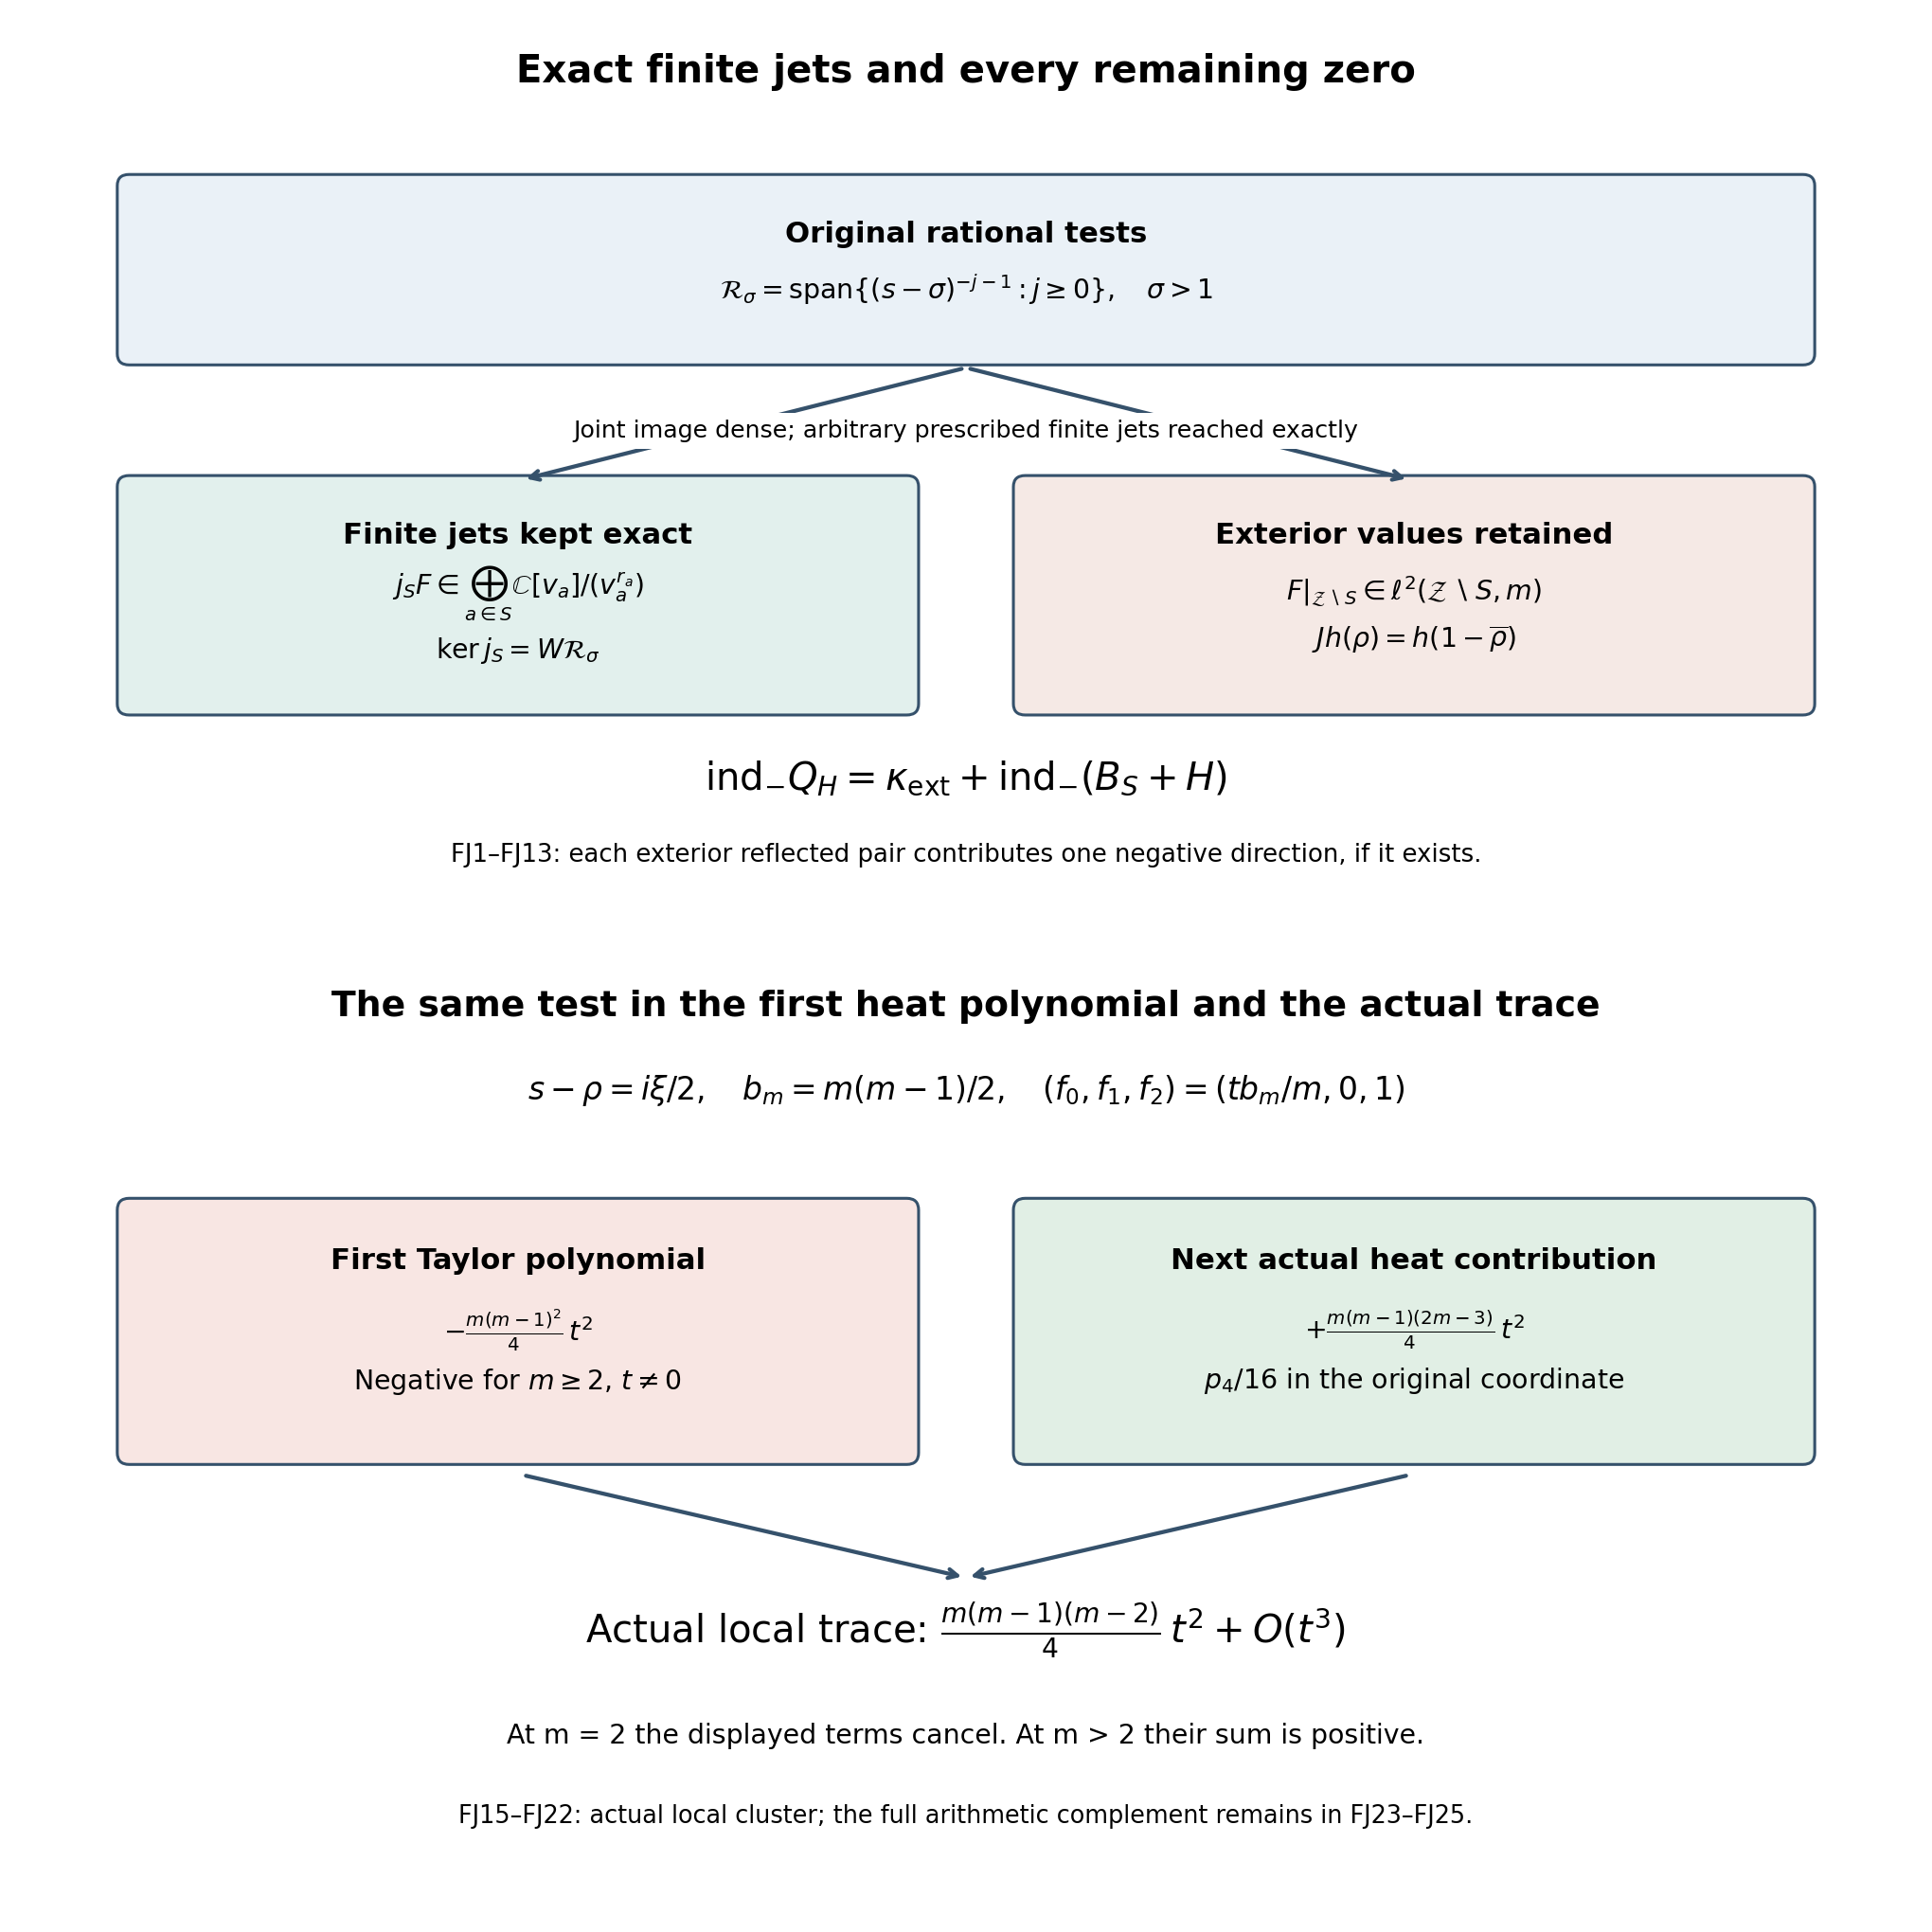
\includegraphics[width=0.95\linewidth,height=\textheight,keepaspectratio,alt={Exact finite-jet and exterior maps, with the retained first and second heat coefficients. FJ1--FJ14 prove the upper diagram; FJ15--FJ22 prove the original-coordinate calculation below. Every endpoint and support coordinate remains in FJ23--FJ29.}]{finite_jet_exterior_heat.png}
\caption{Exact finite-jet and exterior maps, with the retained first and
second heat coefficients. FJ1--FJ14 prove the upper diagram; FJ15--FJ22
prove the original-coordinate calculation below. Every endpoint and
support coordinate remains in FJ23--FJ29.}
\end{figure}

\subsection{Sources and proof
locations}\label{sources-and-proof-locations}

The original heat convention is Brad Rodgers and Terence Tao,
\href{https://arxiv.org/abs/1801.05914v5}{\emph{The de Bruijn--Newman
constant is non-negative}, arXiv:1801.05914v5}, original author
equations \texttt{hoz}, \texttt{htdef}, \texttt{sas}. The entire
original author archive and precise reading coverage are retained with
AG. The supported explicit formula uses Alain Connes,
\href{https://arxiv.org/abs/math/9811068v1}{\emph{Trace formula in
noncommutative geometry and the zeros of the Riemann zeta function},
arXiv:math/9811068v1}, Appendix II Theorem 6, through the complete SZW
proof linked above. The programme proofs
\href{ACTUAL_HEAT_ZERO_DISTRIBUTION_VARIATION.md}{AG1--AG24},
\href{HEAT_CAUCHY_ARITHMETIC_DERIVATION.md}{HA1--HA26},
\href{CAUCHY_WEIL_POSITIVITY_CRITERION.md}{CK1--CK19}, and
\texttt{FIXED\_\allowbreak{}ARITHMETIC\_\allowbreak{}HEAT\_\allowbreak{}FLAGS.\allowbreak{}tex}, HR1--HR18, are included in
the same publication package. The finite Hermite interpolation,
Cauchy-transform density, inertia and second-coefficient calculations
needed here are proved in full above; no historical novelty claim is
made for the classical methods.

\subsection{One fixed primitive test and the entire prime
window}\label{one-fixed-primitive-test-and-the-entire-prime-window-3}

The \href{PRIME_PROJECTOR_MOBIUS_DERIVATION.md}{prime-operator
calculation}, PM1--41, proves both distinct Fourier support corrections
and their exact map into the full Weil formula. The
\href{PRIMITIVE_SHORT_SUPPORT_DERIVATION.md}{local estimate}, PS1--21,
gives a positive translation-difference remainder. The
\href{UNIVERSAL_PRIMITIVE_TRANSLATION_CRITERION.md}{fixed-test proof},
UP1--35, constructs one compact test whose transform is nonzero at every
possible off-critical zero. The
\href{PRIMITIVE_PRIME_WINDOW_DERIVATION.md}{complete arithmetic
calculation}, PW1--22, expresses its entire translated correlation
through a fixed-width prime window and an explicit archimedean
remainder. Its boundedness is equivalent to RH; that bound remains
unresolved. All boundary coordinates and supported-zero labels remain
explicit.

\clearpage

\section{The von Mangoldt operator, Fourier support defects, and the
full Weil
receiver}\label{the-von-mangoldt-operator-fourier-support-defects-and-the-full-weil-receiver}

\textbf{Original-zeta receiving calculation.} The working meromorphic
function is the original Riemann zeta, with its full Gamma/endpoints
multiplier and its full trivial-zero and pole divisor retained.
\href{FAITHFUL_THETA_COMPLETION_RETURN.md}{TF1--42} proves the original
labelled theta inverse and the actual heat-image defect.
\href{FAITHFUL_UNCOMPLETED_ZETA_HEAT.md}{UZ1--53} proves every
exceptional-point fibre, jet, original-zeta heat term and reflection
orientation.
\href{ORIGINAL_ZETA_COMPACT_WEIL_RECONSTRUCTION.md}{OZC1--48} rederives
the compact contour and interval operator directly from zeta, including
the left-cutoff Gamma boundary, and specifies exactly which compensated
pairing the bounds concern.
\href{ORIGINAL_ZETA_HEAT_CONTACT_RECONSTRUCTION.md}{OZH1--49} rederives
the actual meromorphic heat, rational signed trace, compact-test domain,
contact drift and full causal arithmetic variation. The raw full divisor
and the compensated Weil receiver are linked by their displayed
correction, not identified. In particular the fixed-test trivial-zero
sum converges exactly at translations at least 1/32 and equals the
earlier R term; at zero translation it requires the proved cutoff
compensation. \href{ORIGINAL_ZETA_CAUCHY_RECONSTRUCTION.md}{OZK1--38}
reconstructs the original signed Cauchy trace, its full Gamma
correction, resonant finite parts, every finite matrix and its index,
and the complete local heat jets. Its invertible map retains the raw
trace and correction separately. These complete receiving proofs govern
the interpretation of the retained auxiliary calculations below.

This derivation uses the original basis and time scale of
\href{HURWITZ_CYCLOTOMIC_RECEIVER.tex}{HCR1--42, complete companion
source}. It constructs the exact divisibility-projector sum for the von
Mangoldt operator, both of its different supported corrections, and its
map into the complete Weil formula. The resulting translation form has
both signs even after both endpoint values are forced to vanish. No sign
of the entire Weil form is inferred from the positive diagonal operator.

\subsection{1. Objects and the finite arithmetic
identity}\label{objects-and-the-finite-arithmetic-identity}

Let \(\mathbb N=\{1,2,\ldots\}\), \(\mathcal H=\ell^2(\mathbb N)\), and
retain the orthonormal basis \(\xi_n\). Let \(N\xi_n=n\xi_n\) and
\(P_d\xi_n=\mathbf1_{d\mid n}\xi_n\). Thus \(P_d=S_dS_d^*\) in HCR1--4,
with no change to the index or the logarithmic generator \(H=\log N\).
Write \[
\mu(1)=1,\qquad
\mu(n)=\begin{cases}(-1)^r,&n\text{ is a product of }r\text{ distinct primes},\\0,&n\text{ has a squared prime factor},\end{cases}
\quad
\Lambda(n)=\begin{cases}\log p,&n=p^k,\ k\ge1,\\0,&\text{otherwise}.
\end{cases}
\tag{PM1}
\] In particular \(\Lambda(1)=0\). For an integer \(D\ge1\), put \[
I_D=\{d:2\le d\le D,\ \mu(d)\ne0\},\qquad
c_d=-\mu(d)\log d,\qquad
A_D=\sum_{d\in I_D}c_dP_d,
\quad a_D(n)=\sum_{\substack{d\in I_D\\d\mid n}}c_d.
\tag{PM2}
\] Every coefficient in this displayed sum is nonzero. An empty sum is
the zero operator. Each \(A_D\) is a bounded self-adjoint operator: it
is a finite real linear combination of bounded orthogonal projections,
all diagonal in the same basis.

For every \(n\ge1\), \[
\boxed{\Lambda(n)=-\sum_{d\mid n}\mu(d)\log d.}
\tag{PM3}
\] Here and below \(\log1=0\). To prove (PM3), let \(p_1,\ldots,p_r\) be
the distinct prime factors of \(n>1\). Only their squarefree products
contribute. The coefficient of \(\log p_i\) in
\(\sum_{d\mid n}\mu(d)\log d\) is \[
\sum_{J\subset\{1,\ldots,r\}\setminus\{i\}}(-1)^{1+|J|}
=-(1-1)^{r-1}.
\] For \(r=1\) this is \(-1\); for \(r>1\) it is zero. This is exactly
(PM3). For \(n=1\) the sole divisor contributes zero. Consequently
\(a_D(n)=\Lambda(n)\) as soon as \(D\ge n\). No infinite arithmetic sum
is needed at a fixed entry.

\subsection{2. The precise operator domains and modes of
convergence}\label{the-precise-operator-domains-and-modes-of-convergence}

Define the multiplication operator \[
\mathcal D_\Lambda=\left\{x\in\ell^2(\mathbb N):
\sum_n\Lambda(n)^2|x_n|^2<\infty\right\},\qquad
(Ax)_n=\Lambda(n)x_n.
\tag{PM4}
\] It is positive and self-adjoint. Positivity follows by summing the
nonnegative quantities \(\Lambda(n)|x_n|^2\); that series is finite on
\(\mathcal D_\Lambda\) by Cauchy--Schwarz. To identify the adjoint, test
against each basis vector. A vector \(y\) belongs to the adjoint domain
exactly when the sequence \((\Lambda(n)y_n)_n\) is square summable, and
the adjoint is multiplication by that sequence. This is precisely (PM4).
For \(x\in\mathcal D_\Lambda\), its first \(K\) coordinates converge to
\(x\) in both Hilbert norm and the norm of \(Ax\). Thus the finite
vectors form a core. On this core, (PM3) proves the exact identity \[
\boxed{\Lambda(N)=-\sum_{\substack{d\ge2\\\mu(d)\ne0}}
\mu(d)\log(d)P_d,}
\tag{PM5}
\] where the right side stabilizes on each finite vector and its closure
is the operator (PM4).

The convergence assertion cannot be strengthened to strong convergence
of \(A_Dx\) for every \(x\in\mathcal D_\Lambda\). This has an explicit
counterexample. Choose distinct odd primes \(q_j\) so large that
\(\log q_j\ge j^2\), and define \[
x_{2q_j}=1/j,\qquad x_n=0\text{ otherwise}.
\tag{PM6}
\] Arbitrarily large primes exist: a prime divisor of one plus the
product of any finite set of primes is outside that set. Thus this
choice is available. The series \(\sum1/j^2\) converges, and
\(\Lambda(2q_j)=0\), so \(x\in\mathcal D_\Lambda\) and \(Ax=0\). At
cutoff \(D=q_j\), the divisors \(2,q_j\) contribute to its \(2q_j\)
coordinate and \(2q_j\) does not. Hence \[
a_{q_j}(2q_j)=\log(2q_j),\qquad
\|A_{q_j}x\|\ge\log(2q_j)/j\ge j.
\tag{PM7}
\] The claimed stronger convergence therefore fails even on the kernel
of \(A\).

A useful valid common domain is explicit. Set \[
b(1)=0,\qquad
b(n)=\sum_{d\mid n}|\mu(d)|\log d
=2^{\omega(n)-1}\log\operatorname{rad}(n)\quad(n>1),
\quad
\mathcal D_b=\left\{x:\sum b(n)^2|x_n|^2<\infty\right\}.
\tag{PM8}
\] Here \(\omega(n)\) counts its distinct prime factors and
\(\operatorname{rad}(n)\) is their product. Each factor appears in
exactly \(2^{\omega(n)-1}\) squarefree divisors, proving the formula for
\(b\). The bounds \(|a_D(n)|\le b(n)\) and \(\Lambda(n)\le b(n)\),
followed by dominated convergence of the series of squared coordinates,
prove \(A_Dx\to Ax\) for every \(x\in\mathcal D_b\). This statement
preserves the actual cutoff in (PM2).

\subsection{3. The weighted trace and its exact
factor}\label{the-weighted-trace-and-its-exact-factor}

Fix \(s\in\mathbb C\) with \(\sigma=\Re s>1\), using the real logarithm
for \(n^{-s}\). The diagonal operator \(P_dN^{-s}\) has trace norm \[
\|P_dN^{-s}\|_1=\sum_{k\ge1}(dk)^{-\sigma}
=d^{-\sigma}\zeta(\sigma),\qquad
\operatorname{Tr}(P_dN^{-s})=d^{-s}\zeta(s).
\tag{PM9}
\] These are HCR26--28 with \(q=a=d\), also proved directly by their
displayed sums. Therefore \[
\sum_{d\ge2,\,\mu(d)\ne0}|c_d|\,\|P_dN^{-s}\|_1
\le\zeta(\sigma)\sum_{d\ge2}(\log d)d^{-\sigma}<\infty.
\tag{PM10}
\] The scalar majorant converges, for example by integrating
\((\log x)x^{-\sigma}\) on \([2,\infty)\). Thus the weighted operator
series converges in trace norm. Its diagonal entries stabilize to
\(\Lambda(n)n^{-s}\), which identifies its limit as \(AN^{-s}\). In
particular \[
\begin{aligned}
\operatorname{Tr}(AN^{-s})
&=\sum_{n\ge2}\Lambda(n)n^{-s}
=\zeta(s)\sum_{d\ge2}(-\mu(d)\log d)d^{-s}
=-\frac{\zeta'(s)}{\zeta(s)},\\
\|A_DN^{-s}-AN^{-s}\|_1
&\le\zeta(\sigma)\sum_{d>D}|\mu(d)|(\log d)d^{-\sigma}.
\end{aligned}
\tag{PM11}
\] For completeness the last analytic identity follows without
differentiating a conditionally convergent series. The elementary
divisor identity \(\sum_{d\mid n}\mu(d)=\mathbf1_{n=1}\), proved by
\((1-1)^{\omega(n)}\), and absolute Dirichlet convolution give
\(\zeta(s)\sum\mu(d)d^{-s}=1\) for \(\Re s>1\). The two series and their
derivatives converge locally uniformly there, using the same logarithmic
majorants as (PM10). Differentiate \(\sum\mu(d)d^{-s}=1/\zeta(s)\),
obtaining \(\sum(-\mu(d)\log d)d^{-s}=-\zeta'(s)/\zeta(s)^2\), and
multiply by \(\zeta(s)\). In particular all signs in (PM11) are fixed.
This is the function \(-r(s)\) of HA10.

\subsection{4. The original lattice and the two different cutoff
corrections}\label{the-original-lattice-and-the-two-different-cutoff-corrections}

Retain a nontrivial bounded distributive lattice \(L\), with bottom
\(0_L\) and top \(1_L\), and exactly HCR7: \[
\begin{gathered}
G_L(\mathbb C)=\{(a,\lambda):a\ne0\Longrightarrow\lambda=1_L\},\\
(a,\lambda)+(b,\eta)=(a+b,\lambda\vee\eta),\qquad
(a,\lambda)(b,\eta)=(ab,\lambda\wedge\eta),\\
\tau=(0,0_L),\qquad e=(0,1_L),\qquad\widehat c=(c,1_L).
\end{gathered}
\tag{PM12}
\] All matrices below have off-diagonal entries \(\tau\), so they are in
the row-and-column-finite matrix semiring of HCR7--9. Let \[
(\widehat P_d)_{nn}=\begin{cases}1_S,&d\mid n,\\\tau,&d\nmid n,\end{cases}
\quad
(M_d)_{nn}=\begin{cases}\tau,&d\mid n,\\e,&d\nmid n,\end{cases}
\quad
R_d=\widehat{1/d}\sum_{j=0}^{d-1}\widehat E(j/d).
\tag{PM13}
\] The root sum from HCR3, calculated with the actual labels, gives \[
R_d=\widehat P_d+M_d,
\qquad (R_d)_{nn}=(\mathbf1_{d\mid n},1_L).
\tag{PM14}
\] At a nonmultiple the roots cancel in amplitude, and their sum is
\(e\), not \(\tau\).

For \(D\ge2\), define the sparse and raw sums using only the nonzero
coefficients specified in (PM2): \[
\mathcal A_D=\sum_{d\in I_D}\widehat c_d\widehat P_d,
\qquad \mathcal R_D=\sum_{d\in I_D}\widehat c_d R_d,
\quad
\chi_D(n)=\mathbf1_{\exists p\le D:\ p\text{ prime},\ p\mid n}.
\tag{PM15}
\] Then the full entry formulas are \[
(\mathcal A_D)_{nn}=\begin{cases}(a_D(n),1_L),&\chi_D(n)=1,\\\tau,&\chi_D(n)=0,\end{cases}
\qquad
(\mathcal R_D)_{nn}=(a_D(n),1_L).
\tag{PM16}
\] Indeed an active squarefree divisor of \(n\) exists exactly when a
prime divisor at most \(D\) exists. The sparse sum then joins at least
one top label, including when its amplitudes subsequently cancel. Every
raw summand has top diagonal label, and there is at least one such
summand since \(2\in I_D\). This proves (PM16) at every entry. For
\(D=1\) both sums are the zero matrix; it is a separate empty-sum case.

The least missing-support correction is \[
(\mathcal M_D)_{nn}=\begin{cases}\tau,&\chi_D(n)=1,\\e,&\chi_D(n)=0,\end{cases}
\qquad
\boxed{\mathcal A_D+\mathcal M_D=\mathcal R_D.}
\tag{PM17}
\] Every correction \(C\) satisfying \(\mathcal A_D+C=\mathcal R_D\) has
zero amplitudes, off-diagonal entries \(\tau\), top diagonal label when
\(\chi_D(n)=0\), and any original label when \(\chi_D(n)=1\). These
conditions are necessary by amplitude equality and by the joins in
(PM12); they are sufficient by the same calculation. Thus (PM17) is the
unique least correction in the entrywise order on zero-amplitude labels,
and the entire family of corrections has been specified.

The actual sum of the individual Fourier corrections is usually larger.
Put \[
\mathcal K_D=\sum_{d\in I_D}\widehat c_dM_d,
\qquad Q_D=\prod_{p\le D,\ p\text{ prime}}p.
\tag{PM18}
\] Each nonzero \(c_d\) acts on \(e\) as \(e\). Therefore \[
(\mathcal K_D)_{nn}=\begin{cases}\tau,&Q_D\mid n,\\e,&Q_D\nmid n,\end{cases}
\qquad
\boxed{\mathcal A_D+\mathcal K_D=\mathcal R_D.}
\tag{PM19}
\] To prove the first formula, all the active \(d\) divide \(n\) exactly
when all primes at most \(D\) divide \(n\): the forward implication uses
that each of these primes is active, and the reverse uses that an active
\(d\) is squarefree. The second formula follows by adding (PM14) with
its stated coefficients, or directly from (PM16). In particular
\(\mathcal M_D\le\mathcal K_D\), but equality need not hold. For
\(D=3\), at \(n=2\) the least correction is \(\tau\) and the directly
summed correction is \(e\). The additional \(e\) is absorbed by the
already top-labelled entry of \(\mathcal A_D\); it has not been set
equal to \(\tau\).

\subsection{5. All limiting support, including the index
one}\label{all-limiting-support-including-the-index-one}

Every limit in this paragraph is eventual equality at each matrix entry,
so it requires no completeness assumption or infinite join in \(L\). The
exact limits are \[
\begin{aligned}
\mathcal A_{nn}&=\begin{cases}\tau,&n=1,\\(\Lambda(n),1_L),&n\ge2,\end{cases}
&\mathcal R_{nn}&=(\Lambda(n),1_L)\quad(n\ge1),\\
\mathcal M_{nn}&=\begin{cases}e,&n=1,\\\tau,&n\ge2,\end{cases}
&\mathcal K&=Z=\operatorname{diag}(e,e,\ldots).
\end{aligned}
\tag{PM20}
\] For \(n\ge2\), some prime divisor appears by \(D\ge n\), and (PM3)
fixes the amplitude. The index 1 has no active divisors. For the last
limit choose a prime not dividing the fixed integer \(n\); once it is
included, \(Q_D\nmid n\) forever. Existence follows from the elementary
infinitude argument already supplied. Thus \[
\boxed{\mathcal A+\mathcal M=\mathcal R=\mathcal A+Z.}
\tag{PM21}
\] In particular every integer with at least two distinct prime factors
has the entry \(e\) in both \(\mathcal A\) and \(\mathcal R\), since its
zero value of \(\Lambda\) was produced by cancellation. Only the sparse
index 1 has \(\tau\). The least limiting defect and the directly summed
limiting defect are different matrices, even though both complete the
same equation.

The stipulated index set is also essential to the full lift. In the
complex identity one may insert the zero term \(-\mu(1)\log1\,P_1=0\).
Lifting that newly inserted coefficient as \(\widehat0=e\) instead gives
\(e\widehat P_1=Z\), since \(P_1=I\). Thus adding this zero term before
lifting changes the sparse lift from \(\mathcal A\) to
\(\mathcal A+Z=\mathcal R\). This is the exact connecting map for the
two presentations, not permission to identify their support matrices.
The original index set \(d\ge2,\mu(d)\ne0\) in (PM5) has been retained
throughout.

For an arbitrary input with original coordinates
\(v_n=(x_n,\lambda_n)\), where \(x\in\ell^2\) and
\(x_n\ne0\Rightarrow\lambda_n=1_L\), the finite sums act by \[
(\mathcal A_Dv)_n=
\begin{cases}(a_D(n)x_n,\lambda_n),&\chi_D(n)=1,\\\tau,&\chi_D(n)=0,\end{cases}
\quad
(\mathcal R_Dv)_n=(a_D(n)x_n,\lambda_n).
\tag{PM22}
\] Their amplitude operators are bounded at each finite \(D\). The
limiting amplitude operator has domain (PM4). On that domain the
limiting labelled maps act as \((\Lambda(n)x_n,\lambda_n)\) at every
\(n\ge2\), with \(\tau\) at 1 for the sparse map and \((0,\lambda_1)\)
at 1 for the raw map. This is an entrywise definition with the domain of
the amplitude stated; it does not assert the false Hilbert convergence
excluded in (PM7).

The complete coefficient injection of HCR9 sends a matrix entry
\((a,\lambda)\) to \((a,\iota_L(\lambda))\), where
\(\iota_L:L\hookrightarrow K\otimes_{\mathbb B}L\) has its stated
retraction. For diagonal masks write \(\chi_D^K\) and \((1-\chi_D)^K\)
for the separate selected and complementary indicators; the notation is
a description of masks, not subtraction in the lattice semiring. The
exact images are \[
\begin{array}{c|cc}
&\text{complex amplitude}&\text{full support matrix}\\\hline
\mathcal A_D&A_D&\chi_D^K\\
\mathcal R_D&A_D&I_K\\
\mathcal M_D&0&(1-\chi_D)^K\\
\mathcal K_D&0&\mathbf1_{Q_D\nmid n}^{K}
\end{array}
\tag{PM23}
\] The same map takes the limits to the corresponding masks in (PM20).
The retraction recovers every original label, including the
\(\lambda_n\) in (PM22). The common-label completion \(C(D)=D+Z\) of
HCR16 sends \(\mathcal A_D\) to \(\mathcal R_D\) and \(\mathcal A\) to
\(\mathcal R\). Its kernel congruence is equality of amplitudes; the
complete injection (PM23) has not taken that quotient.

There is also a supported weighted trace, with its domain expressly
fixed. For \(\Re s>1\), multiply the diagonal entries by
\((n^{-s},1_L)\), take finite basis traces, and then take the absolutely
convergent amplitude limit while retaining the eventual label. For
\(D\ge2\), sparse finite basis traces are \(\tau\) at cutoff 1 and
top-labelled at every cutoff at least 2. Raw traces are top-labelled at
every positive cutoff. Hence both limiting traces are \[
\left(\operatorname{Tr}(A_DN^{-s}),1_L\right),
\quad\text{and, as }D\to\infty,\quad
\left(-\zeta'(s)/\zeta(s),1_L\right).
\tag{PM24}
\] The correction traces are \(e\), because their zero-amplitude support
contains index 1. Equality of the two scalar traces thus does not
identify their different support matrices. This construction does not
define a trace on arbitrary infinite labelled matrices.

\subsection{6. The exact map into the complete Weil prime
distribution}\label{the-exact-map-into-the-complete-weil-prime-distribution}

Use the original SZW19 convention \[
\mathcal T=C_c^\infty(\mathbb R;\mathbb C),\quad
M_h(s)=\int_{\mathbb R}h(v)e^{-(s-1/2)v}\,dv,
\quad h^\#(v)=\overline{h(-v)}.
\tag{PM25}
\] For \(h\in\mathcal T\), the diagonal operator \[
B_h=N^{-1/2}\{h(\log N)+h(-\log N)\}
\tag{PM26}
\] has finite rank: if \(\operatorname{supp}h\subset[-R,R]\), its
entries vanish for \(n>e^R\). Its entry at 1 is \(2h(0)\). Since
\(\Lambda(1)=0\), the exact trace receiver is \[
\begin{aligned}
\operatorname{Tr}(AB_h)
&=\sum_{n\ge2}\frac{\Lambda(n)}{\sqrt n}
\{h(\log n)+h(-\log n)\}\\
&=\sum_p\sum_{k\ge1}(\log p)p^{-k/2}
\{h(k\log p)+h(-k\log p)\}
=P_{\rm fin}(h).
\end{aligned}
\tag{PM27}
\] The prime-power expansion uses (PM1), not an altered norm for
supported zero. Every sum in (PM27) is finite for a fixed test. At
cutoff \(D\ge\max(2,\lfloor e^R\rfloor)\), \(\operatorname{Tr}(A_DB_h)\)
is already equal to (PM27).

To state a full supported test receiver rather than hiding its choices,
take \(K\ge\max(2,\lfloor e^R\rfloor)\) and the specified finite-basis
lift \[
(\widehat B_{h,K})_{nn}=
\begin{cases}(n^{-1/2}\{h(\log n)+h(-\log n)\},1_L),&1\le n\le K,\\
\tau,&n>K.
\end{cases}
\tag{PM28}
\] It keeps the zero values inside that chosen finite basis as \(e\).
Multiplying by the matrices in (PM20), followed by the finite trace,
gives \[
\operatorname{tr}(\mathcal A\widehat B_{h,K})
=\operatorname{tr}(\mathcal R\widehat B_{h,K})
=(P_{\rm fin}(h),1_L),
\quad
\operatorname{tr}(\mathcal M\widehat B_{h,K})=e.
\tag{PM29}
\] The first top label in the sparse trace is at index 2; the raw trace
already has it at index 1. These assertions remain true if \(h=0\),
because (PM28) deliberately specifies a top-labelled lift of its zero
values. This lift therefore is not asserted to be an additive
zero-preserving linear map from the complex test space into the ambient
split semiring. The amplitude trace is the complex-linear distribution
(PM27); the complete matrix injection (PM23) separately retains the
support. If a support-adapted lift of \(B_h\) is chosen instead, its
zero entries have different labels and (PM28)--(PM29) must not be
silently reused.

The connection to the entire supported formula is now exact. With
\(H=M_h\), let \(\mathbf e_\lambda\) denote the coordinate basis of
\(\mathbb C[L]\) for the finite support lattice used in SZW. Its
existing identity is \[
\begin{aligned}
\boldsymbol B_L(h)&=(H(0)+H(1))\mathbf e_{1_L}
 +H(0)\sum_{\lambda\ne1_L}\mathbf e_\lambda,\\
\boldsymbol Z_L(h)&=Z(h)\mathbf e_{1_L},\\
\boldsymbol D_L(h)&=(\operatorname{Tr}(AB_h)-A_\infty(h))\mathbf e_{1_L}
 +H(0)\sum_{\lambda\ne1_L}\mathbf e_\lambda,\\
\boldsymbol B_L(h)-\boldsymbol Z_L(h)&=\boldsymbol D_L(h),
\end{aligned}
\tag{PM30}
\] where \[
Z(h)=\sum_\rho m_\rho M_h(\rho),\qquad
A_\infty(h)=\frac1{2\pi}\int_{\mathbb R}\widehat h(t)
\{\Re\psi(1/4+it/2)-\log\pi\}\,dt.
\tag{PM31}
\] Here the sum ranges over all nontrivial zeta zeros with their
multiplicities and \(\widehat h(t)=\int h(v)e^{-itv}dv\). Formula (PM30)
follows by substituting the proved equality (PM27) into SZW24--25 and
SZW33--34. Those original formulas retain the theta endpoint traces and
prove their convergence. No lower coordinate is replaced by a proposed
numerical prime weight. For the noncompact Cauchy convolution in HA7,
the same receiver is an absolutely convergent trace: its two terms at
\(\pm\log n\) give precisely \((n^{-w}+n^{-\bar z})/(w+\bar z-1)\),
yielding the prime term of HA11 when \(\Re z,\Re w>1\). Thus (PM11),
(PM27), and HA11 receive exactly the same arithmetic coefficients with
their original constants.

\subsection{7. Translation is the map relevant to
positivity}\label{translation-is-the-map-relevant-to-positivity}

For \(f,g\in\mathcal T\), direct substitution in convolution gives \[
(f^\#*g)(v)=\int_{\mathbb R}\overline{f(x)}g(x+v)\,dx
=\langle f,U_vg\rangle_{L^2(\mathbb R)},\qquad
(U_vg)(x)=g(x+v),\quad U_v^*=U_{-v}.
\tag{PM32}
\] If the difference of the two test supports is contained in
\([-R,R]\), all terms outside that interval vanish, and \[
P_{\rm fin}(f^\#*g)
=\left\langle f,
\sum_{2\le n\le e^R}\frac{\Lambda(n)}{\sqrt n}
\{U_{\log n}+U_{-\log n}\}g\right\rangle.
\tag{PM33}
\] The finite operator on the right is bounded and self-adjoint; its
norm is at most \(2\sum_{n\le e^R}\Lambda(n)/\sqrt n\). The expression
stabilizes on each fixed test pair as \(R\) grows. An infinite bounded
translation operator is not required or asserted. This is the exact
receiver from the positive multiplication operator (PM4) to the prime
sesquilinear form. The map from finite diagonal coefficients to the sum
of translations in (PM33) is linear and respects adjoints, but is not a
positive map.

Here is a complete sign test. Write \(a=\log2\), choose \[
0<2\delta<\min\{\log2,\log(3/2)\},\qquad
0\ne\varphi\in C_c^\infty((-\delta,\delta)),\qquad
\varphi_a(x)=\varphi(x-a).
\tag{PM34}
\] For any nonzero \(\eta\) with this support, put \(k=\eta^\#*\eta\)
and \(g_\pm=\eta\pm\eta_a\). Then \[
g_\pm^\#*g_\pm(v)=2k(v)\pm k(v-a)\pm k(v+a),
\quad k(0)=\|\eta\|_2^2,
\quad\operatorname{supp}k\subset[-2\delta,2\delta].
\tag{PM35}
\] Indeed expand the four convolutions in (PM32); translating both
arguments leaves \(k\) unchanged and translating one shifts it by
\(\pm a\). At \(v=a\) or \(-a\), only one shifted term survives, giving
\(\pm\|\eta\|_2^2\). At \(v=\pm\log n\) with \(n\ge3\), every term
vanishes because \(a+2\delta<\log3\). Consequently \[
\boxed{P_{\rm fin}(g_\pm^\#*g_\pm)
=\pm\frac{2\log2}{\sqrt2}\|\eta\|_2^2
=\pm\sqrt2\log2\,\|\eta\|_2^2.}
\tag{PM36}
\] This also proves nonpositivity of the coefficient-to-translation map
already on the positive single diagonal coefficient at index 2. Positive
diagonal coefficients alone therefore do not imply a positive
autocorrelation receiver.

\subsection{8. The same exact signs survive endpoint
annihilation}\label{the-same-exact-signs-survive-endpoint-annihilation}

Keep the test operator and its original constant \[
T=\partial_v^2-\tfrac14.
\tag{PM37}
\] Integration by parts twice, with no boundary term for a compact
smooth test, gives \[
M_{Tf}(s)=\bigl((s-\tfrac12)^2-\tfrac14\bigr)M_f(s)
=s(s-1)M_f(s).
\tag{PM38}
\] Thus both endpoint values vanish exactly; at every nontrivial zero
the multiplying factor is nonzero. The coefficients are real and the
order is even, so \((Tf)^\#=T(f^\#)\). Differentiation of compact
convolution gives \[
(Tf)^\#*(Tg)=T^2(f^\#*g),\qquad
M_{(Tf)^\#*(Tg)}(s)=[s(s-1)]^2
\overline{M_f(1-\bar s)}M_g(s).
\tag{PM39}
\] All support and convergence requirements of (PM27) and (PM30)
continue to hold.

For an explicit endpoint-zero version of (PM36), take \(\eta=T\varphi\)
with \(\varphi\) from (PM34). This \(\eta\) is nonzero. Otherwise
\(\varphi''=\varphi/4\) everywhere; solving this equation with its zero
value and zero derivative outside the compact support gives the
identically zero solution, a contradiction. Its support remains
contained in \((-\delta,\delta)\), and \(T\) commutes with translation.
Hence \[
g_\pm=T(\varphi\pm\varphi_a),\quad
M_{g_\pm}(0)=M_{g_\pm}(1)=0,\quad
\boxed{P_{\rm fin}(g_\pm^\#*g_\pm)
=\pm\sqrt2\log2\,\|T\varphi\|_2^2.}
\tag{PM40}
\] There is no approximation in these signs, and no zero-location
assumption in their proof.

For these or any endpoint-zero tests, write \(h=g^\#*g\). Then
\(M_h(0)=M_h(1)=0\) by the convolution formula, so (PM30) is exactly \[
\boldsymbol B_L(h)=0,\quad
\boldsymbol D_L(h)=(P_{\rm fin}(h)-A_\infty(h))\mathbf e_{1_L},\quad
\boldsymbol Z_L(h)=(A_\infty(h)-P_{\rm fin}(h))\mathbf e_{1_L}.
\tag{PM41}
\] The coordinate spaces and all support maps remain those of (PM30);
the lower coefficients here are the calculated zero values of these
tests. In particular (PM40) assigns no sign to (PM41) until the
archimedean term is included. The exact remaining comparison is between
the archimedean form and the translated prime form, with their already
fixed constants. The positive operator \(\Lambda(N)\), the raw supported
zeros, and the endpoint annihilator each have now been connected to that
comparison by explicit maps rather than by a positivity assertion.

\subsection{Source identities and actual reading
coverage}\label{source-identities-and-actual-reading-coverage}

\begin{itemize}
\tightlist
\item
  \textbf{HCR:}
  \texttt{work/\allowbreak{}rh\_\allowbreak{}counterfactual\_\allowbreak{}20260913/\allowbreak{}tau\_\allowbreak{}prime\_\allowbreak{}weil\_\allowbreak{}20260922/\allowbreak{}cc\_\allowbreak{}totality\_\allowbreak{}20260923/\allowbreak{}reader\_\allowbreak{}fragments/\allowbreak{}HURWITZ\_\allowbreak{}CYCLOTOMIC\_\allowbreak{}RECEIVER.\allowbreak{}tex},
  SHA256
  \texttt{d8a4caa0\allowbreak{}b66e492e\allowbreak{}7ffe987b\allowbreak{}a2aa04be\allowbreak{}b201aed3\allowbreak{}cacc3b30\allowbreak{}a3b0d4b5\allowbreak{}26e6df38}.
  Read the complete HCR1--42 and their proofs for this derivation.
  Operators and full lattice are HCR1--16; the weighted original trace
  is HCR26--31. Its human operator source is Alain Connes, Caterina
  Consani and Matilde Marcolli,
  \href{https://arxiv.org/abs/0806.2401v1}{\emph{Fun with F1},
  arXiv:0806.2401v1}, original \texttt{funBC.\allowbreak{}tex}, relations
  \texttt{pres}, \texttt{idem}, \texttt{endo}, \texttt{endosigma}, and
  (c1)--(c4), with exact line ranges recorded in HCR. This derivation
  has read the HCR proof, not newly reread that author archive; HCR's
  original-source reading claim is not represented as a new reading
  here. Equations (PM13)--(PM19) reprove every operator and label
  identity actually needed.
\item
  \textbf{HA:} \texttt{HEAT\_\allowbreak{}CAUCHY\_\allowbreak{}ARITHMETIC\_\allowbreak{}DERIVATION.\allowbreak{}md}, SHA256
  \texttt{024d3f42\allowbreak{}723fabf2\allowbreak{}361cab94\allowbreak{}00d98d2f\allowbreak{}e64c57ec\allowbreak{}114112e6\allowbreak{}ada6f543\allowbreak{}0a88f909}.
  Read HA1--26 for this derivation.
  \href{https://github.com/KokunoYumeto/zeta-function-research-reader/blob/76f421965914beb133df797835f940849844dc4f/workbenches/splitzero-tandem/branches/tau-zero-prime-positivity/HEAT_CAUCHY_ARITHMETIC_DERIVATION.md}{HA10--14,
  pinned public proof} supply the exact logarithmic derivative, Cauchy
  trace and supported coefficients checked in (PM11), (PM30), and the
  paragraph after (PM31).
\item
  \textbf{SZW:} \texttt{SUPPORTED\_\allowbreak{}ZERO\_\allowbreak{}PRIME\_\allowbreak{}WEIL\_\allowbreak{}DERIVATION.\allowbreak{}md},
  SHA256
  \texttt{ff7fbe6c\allowbreak{}c6277203\allowbreak{}68a7c245\allowbreak{}052ef826\allowbreak{}3925ca2d\allowbreak{}912046df\allowbreak{}e45e3be7\allowbreak{}4d4455f4}.
  Read SZW19--26 and SZW33--38, with adjacent text, for this derivation.
  The complete explicit-formula proof is in
  \href{https://github.com/KokunoYumeto/zeta-function-research-reader/blob/5a89872598df0902b7c1393cf8e4692ca3010a95/workbenches/splitzero-tandem/branches/tau-zero-prime-positivity/SUPPORTED_ZERO_PRIME_WEIL_DERIVATION.md}{SZW24--26
  and full support identity SZW33--34, pinned public source}. Its human
  explicit-formula source is Alain Connes,
  \href{https://arxiv.org/abs/math/9811068}{\emph{Trace formula in
  noncommutative geometry and the zeros of the Riemann zeta function}},
  Appendix II, Theorem 6. The present proof uses the complete programme
  derivation and does not assert a new reading of that author archive.
\end{itemize}

The Möbius identity (PM3) is the classical arithmetic inversion
identity, proved here with its complete divisor calculation. The new
programme calculation is its specified split lift, both distinct support
corrections and their limits, its exact full Weil receiver, and the
endpoint-zero sign test. No novelty claim about classical Möbius
inversion, trace-class diagonal operators, or the classical explicit
formula is made.

\clearpage

\section{The actual archimedean form on short-support
primitives}\label{the-actual-archimedean-form-on-short-support-primitives}

\textbf{Original-zeta receiving calculation.} The working meromorphic
function is the original Riemann zeta, with its full Gamma/endpoints
multiplier and its full trivial-zero and pole divisor retained.
\href{FAITHFUL_THETA_COMPLETION_RETURN.md}{TF1--42} proves the original
labelled theta inverse and the actual heat-image defect.
\href{FAITHFUL_UNCOMPLETED_ZETA_HEAT.md}{UZ1--53} proves every
exceptional-point fibre, jet, original-zeta heat term and reflection
orientation.
\href{ORIGINAL_ZETA_COMPACT_WEIL_RECONSTRUCTION.md}{OZC1--48} rederives
the compact contour and interval operator directly from zeta, including
the left-cutoff Gamma boundary, and specifies exactly which compensated
pairing the bounds concern.
\href{ORIGINAL_ZETA_HEAT_CONTACT_RECONSTRUCTION.md}{OZH1--49} rederives
the actual meromorphic heat, rational signed trace, compact-test domain,
contact drift and full causal arithmetic variation. The raw full divisor
and the compensated Weil receiver are linked by their displayed
correction, not identified. In particular the fixed-test trivial-zero
sum converges exactly at translations at least 1/32 and equals the
earlier R term; at zero translation it requires the proved cutoff
compensation. \href{ORIGINAL_ZETA_CAUCHY_RECONSTRUCTION.md}{OZK1--38}
reconstructs the original signed Cauchy trace, its full Gamma
correction, resonant finite parts, every finite matrix and its index,
and the complete local heat jets. Its invertible map retains the raw
trace and correction separately. These complete receiving proofs govern
the interpretation of the retained auxiliary calculations below.

This proof gives an explicit rational lower bound, an exact bilinear
representation of its positive remainder, and an exact localization on
primitive functions retaining all cross terms. It uses the original
minus-sign Mellin convention and HA13. No historical novelty claim is
made for short-support Weil positivity or for the endpoint-annihilating
differential operator.

\subsection{PS1. Original tests, correlations and the archimedean
form}\label{ps1.-original-tests-correlations-and-the-archimedean-form}

Let \(f,g\in C_c^\infty(\mathbb R;\mathbb C)\), and retain the
conventions

\[
f^\#(u)=\overline{f(-u)},\qquad
h_{f,g}=f^\#*g,\qquad
M_f(s)=\int_{\mathbb R}f(u)e^{-(s-1/2)u}\,du.
\tag{PS1}
\]

The inner product is \(\langle f,g\rangle=\int\overline{f(u)}g(u)\,du\),
conjugate-linear in its first argument. Define the translation
\(\tau_a f(u)=f(u-a)\). Changing variables in the convolution gives

\[
h_{f,g}(a)=\langle\tau_a f,g\rangle,
\quad h_{f,g}(-a)=\langle f,\tau_a g\rangle,
\quad h_{f,g}(0)=\langle f,g\rangle.
\tag{PS2}
\]

For the diagonal correlation, \(h(-a)=\overline{h(a)}\) and
\(|h(a)|\le h(0)=\|f\|^2\) by Cauchy--Schwarz. If the two functions are
supported in one interval of length \(\ell>0\), their correlation
vanishes outside \([-\ell,\ell]\). This statement does not depend on the
center of the interval.

Use precisely the archimedean functional proved in
\href{https://github.com/KokunoYumeto/zeta-function-research-reader/blob/76f421965914beb133df797835f940849844dc4f/workbenches/splitzero-tandem/branches/tau-zero-prime-positivity/HEAT_CAUCHY_ARITHMETIC_DERIVATION.md}{HA13,
complete public proof}:

\[
\begin{aligned}
\mathcal A(f,g):=A_\infty(h_{f,g})
={}&-(\gamma+\log\pi)\langle f,g\rangle\\
&+\int_0^\infty
\frac{e^{-x}\langle f,g\rangle
-\tfrac12e^{-x/4}(h_{f,g}(x/2)+h_{f,g}(-x/2))}
{1-e^{-x}}\,dx.
\end{aligned}
\tag{PS3}
\]

Here \(\gamma\) is Euler's constant. This is a Hermitian sesquilinear
form on the stated smooth test space. The cancellation of the numerator
at \(x=0\) makes the integral converge; smoothness suffices. No sign
convention for an archimedean geometric distribution is substituted for
PS3: its sign is the archimedean term appearing positively in the
original spectral explicit formula.

\subsection{PS2. Exact bilinear short-support
identity}\label{ps2.-exact-bilinear-short-support-identity}

For \(\ell>0\), set

\[
\begin{aligned}
C(\ell)={}&-\gamma-\log\pi
-\log(1-e^{-2\ell})\\
&+\int_0^{2\ell}\frac{e^{-x}-e^{-x/4}}{1-e^{-x}}\,dx,
\qquad
w(x)=\frac{e^{-x/4}}{1-e^{-x}}.
\end{aligned}
\tag{PS4}
\]

For \(f,g\) supported in one interval of length \(\ell\), the following
is an equality, not merely an inequality:

\[
\boxed{\mathcal A(f,g)=C(\ell)\langle f,g\rangle
+\frac12\int_0^{2\ell}w(x)
\langle\tau_{x/2}f-f,\tau_{x/2}g-g\rangle\,dx.}
\tag{PS5}
\]

To prove it, split PS3 at \(2\ell\). Above that point the two
correlations vanish, while

\[
\int_{2\ell}^\infty\frac{e^{-x}}{1-e^{-x}}\,dx
=-\log(1-e^{-2\ell}).
\]

Below that point use the unitary translation identity

\[
\langle\tau_a f-f,\tau_a g-g\rangle
=2\langle f,g\rangle-h_{f,g}(a)-h_{f,g}(-a).
\]

Its substitution separates the remaining constant multiple of
\(\langle f,g\rangle\), which is exactly the integral in PS4, and leaves
the positive-weight integral in PS5. The latter converges at zero:
\(\|\tau_a f-f\|\le |a|\|f'\|\), obtained by the fundamental theorem of
calculus and Minkowski's inequality. Thus the bilinear integrand is
\(O(x^2)w(x)=O(x)\) there.

In particular, taking the diagonal gives

\[
\mathcal A(f,f)=C(\ell)\|f\|^2
+\frac12\int_0^{2\ell}w(x)
\|\tau_{x/2}f-f\|^2\,dx
\ge C(\ell)\|f\|^2.
\tag{PS6}
\]

The remainder is explicitly a Gram integral of translation differences.
Consequently the same local lower bound holds as a matrix inequality on
every finite family supported in that one common interval. The equality
also proves directly that the proposed \(C(\ell)\) has the correct tail
sign and every factor of two from the original HA13 coordinate.

\subsection{PS3. The rational lower bound
55/192}\label{ps3.-the-rational-lower-bound-55192}

For \(x>0\) put \(q=e^{-x/4}\in(0,1)\). The integrand in PS4 is

\[
\frac{e^{-x}-e^{-x/4}}{1-e^{-x}}
=-\frac{q(1+q+q^2)}{1+q+q^2+q^3}\ge-\frac34.
\tag{PS7}
\]

The final inequality is equivalent to \(q+q^2+q^3\le3\), which holds
term by term. Its limit at zero is \(-3/4\), so the integral has no
unaccounted singular endpoint. Therefore it is at least \(-3\ell/2\).

The elementary inequalities used next can all be retained without
decimal approximations. First \(\gamma\le1\): the decreasing sequence
\(H_n-\log n\) has limit \(\gamma\) and starts at one. Its decrease
follows from \(\log(1+1/n)\ge1/(n+1)\), by integration of \(1/x\) on
\([1,1+1/n]\). Its lower bound follows by comparing the harmonic sum
with the same integral, so this passage to the limit is valid. Second
\(\pi\le4\), for example from containment of the unit disc in the square
of side two. Third,

\[
\log x\ge\frac{2(x-1)}{x+1}\quad(x\ge1),
\]

because the derivative of their difference is \((x-1)^2/[x(x+1)^2]\ge0\)
and the difference is zero at one. At \(x=2\) this yields
\(\log2\ge2/3\), hence \(\log4\ge4/3\).

Finally \(1-e^{-2\ell}\le2\ell\) follows by integrating \(e^{-x}\le1\).
Combining all these inequalities in the correct direction gives

\[
\begin{aligned}
C(\ell)
&\ge-1-\log4-\log(2\ell)-\frac32\ell\\
&=-1+\log\frac1{8\ell}-\frac32\ell\\
&\ge-1+\log4-\frac3{64}
\ge\frac13-\frac3{64}=\frac{55}{192}
\qquad(0<\ell\le1/32).
\end{aligned}
\tag{PS8}
\]

Thus the actual archimedean form satisfies the proved bound

\[
\boxed{\mathcal A(f,f)\ge\frac{55}{192}\|f\|^2}
\tag{PS9}
\]

for any smooth \(f\) supported in an interval of length at most
\(1/32\). No endpoint-vanishing condition is required for this
archimedean assertion. A smooth function supported in a zero-length
interval is zero and satisfies it trivially.

\subsection{PS4. Endpoint-annihilating primitives and the whole Weil
form}\label{ps4.-endpoint-annihilating-primitives-and-the-whole-weil-form}

Retain the original differential operator

\[
T=\frac{d^2}{du^2}-\frac14,
\qquad f=Tg,\quad g\in C_c^\infty(\mathbb R).
\tag{PS10}
\]

Two integrations by parts, with no boundary terms, give

\[
M_{Tg}(s)=\bigl((s-1/2)^2-1/4\bigr)M_g(s)
=s(s-1)M_g(s).
\tag{PS11}
\]

Thus both endpoint values vanish exactly, while \(T\) does not enlarge
the support. Its squared norm, with complex-valued functions permitted,
is exactly

\[
\begin{aligned}
\|Tg\|^2
&=\|g''\|^2-\frac12\Re\langle g'',g\rangle
+\frac1{16}\|g\|^2\\
&=\|g''\|^2+\frac12\|g'\|^2+\frac1{16}\|g\|^2.
\end{aligned}
\tag{PS12}
\]

For a compact test \(f\) write its original reflected Weil form as

\[
\mathcal Q(f,g)=\sum_\rho m_\rho
\overline{M_f(\rho^\#)}M_g(\rho)
=M_{f^\#*g}(0)+M_{f^\#*g}(1)
+\mathcal A(f,g)-P_{\rm fin}(f^\#*g).
\tag{PS13}
\]

The complete underlying formula is
\href{https://github.com/KokunoYumeto/zeta-function-research-reader/blob/76f421965914beb133df797835f940849844dc4f/workbenches/splitzero-tandem/branches/tau-zero-prime-positivity/SUPPORTED_ZERO_PRIME_WEIL_DERIVATION.md}{SZW24--26
and SZW33--38}. The sum converges by the original strip zero count and
rapid Mellin decay; the displayed identity is SZW25 with its original
constants. Its two endpoint values for \(f=Tg\) are zero by PS11 and the
convolution identity. If \(g\) is supported in an interval of length
\(\ell\le1/32\), the correlation of \(Tg\) is supported in
\([-\ell,\ell]\). Since \(\ell<\log2\), every prime term
\(h(\pm\log n)\) with \(n\ge2\) vanishes exactly. Consequently the whole
spectral form in PS13, with endpoints retained and evaluated, equals the
archimedean form and satisfies

\[
\boxed{\mathcal Q(Tg,Tg)\ge\frac{55}{192}
\left(\|g''\|^2+\frac12\|g'\|^2
+\frac1{16}\|g\|^2\right).}
\tag{PS14}
\]

The inequality is strict for \(g\ne0\), since its right side is strictly
positive. This proves the proposed primitive estimate with the exact
positive sign in the original full spectral form. In the
support-resolved SZW identity the endpoint amplitude in every boundary
coordinate is zero for these tests; the labels themselves remain
present. No support element is identified with a scalar zero by this
computation.

For precision, every compact smooth test with both endpoint moments zero
does have a unique compact smooth primitive in this sense. An explicit
inverse, preserving the containing support interval, is

\[
g(u)=-\int_{\mathbb R}e^{-|u-v|/2}f(v)\,dv.
\tag{PS15}
\]

The kernel \(-e^{-|u|/2}\) has first derivative jump one and satisfies
\(TK=\delta_0\) in distributions. Thus \(Tg=f\), and convolution with
smooth compact \(f\) gives a smooth function. If
\(\operatorname{supp}f\subset[a,b]\), then for \(u>b\) its value is
\(-e^{-u/2}M_f(0)=0\), and for \(u<a\) it is \(-e^{u/2}M_f(1)=0\). Hence
\(\operatorname{supp}g\subset[a,b]\). The difference of two compact
primitives solves the homogeneous equation and is a linear combination
of \(e^{u/2}\) and \(e^{-u/2}\); compact support forces both
coefficients to vanish. This proves the stated exact inverse and
uniqueness, not only existence of some endpoint-null images of \(T\).

\subsection{PS5. Exact bilinear localization of the
primitive}\label{ps5.-exact-bilinear-localization-of-the-primitive}

Let \(g\) now be an arbitrary compact smooth function. Choose a finite
smooth partition of unity \(\chi_j\) on a neighborhood of its support,
with each \(\chi_j\) supported in an interval \(I_j\) of length at most
\(1/32\). Such a partition follows by covering the compact support by
finitely many shorter open intervals, choosing nonnegative bumps
positive on a smaller cover, and dividing by their positive sum on a
neighborhood of the support; an auxiliary cutoff inside that
neighborhood makes each resulting function compact smooth. Put

\[
g_j=\chi_jg,\qquad f_j=Tg_j.
\tag{PS16}
\]

These formulas retain the derivatives of the partition:

\[
f_j=\chi_jTg+2\chi_j'g'+\chi_j''g,
\qquad g=\sum_jg_j,\qquad Tg=\sum_jf_j.
\tag{PS17}
\]

The last equality uses \(\sum_j\chi_j=1\),
\(\sum_j\chi_j'=\sum_j\chi_j''=0\) near \(\operatorname{supp}g\);
outside that support all the derivatives of \(g\) vanish. It is
therefore an equality of the original tests, not a replacement by the
functions \(\chi_jTg\) alone.

Each piece has both endpoint moments zero and the stated short support.
For the exact finite Hermitian matrix

\[
q_{jk}=\mathcal Q(f_j,f_k),
\]

sesquilinearity and the finite convolution expansion give

\[
\begin{aligned}
\mathcal Q(Tg,Tg)
&=\sum_{j,k}q_{jk}
=\sum_j q_{jj}+2\Re\sum_{j<k}q_{jk},\\
q_{jk}
&=\mathcal A(f_j,f_k)-P_{\rm fin}(f_j^\#*f_k),\\
q_{jj}
&\ge\frac{55}{192}
\left(\|g_j''\|^2+\frac12\|g_j'\|^2
+\frac1{16}\|g_j\|^2\right).
\end{aligned}
\tag{PS18}
\]

The endpoint terms vanish also for each cross pair, since both primitive
factors have their two endpoint moments zero. The prime term vanishes
for each diagonal, but is retained in every off-diagonal entry. The
exact support relation is

\[
\operatorname{supp}(f_j^\#*f_k)\subset I_k-I_j.
\tag{PS19}
\]

Thus distinct windows can have nonzero prime correlations even though
each window separately has none. PS18 does not infer a sign for the
entire matrix from the positive diagonal terms.

The bilinear primitive and convolution maps also retain their exact
coefficients:

\[
\langle Tg_j,Tg_k\rangle
=\langle g_j'',g_k''\rangle
+\frac12\langle g_j',g_k'\rangle
+\frac1{16}\langle g_j,g_k\rangle,
\tag{PS20}
\]

\[
(Tg_j)^\#*(Tg_k)
=T^2(g_j^\#*g_k),\qquad
T^2=D^4-\frac12D^2+\frac1{16}.
\tag{PS21}
\]

For PS20 integrate the two cross terms by parts separately. For PS21 use
that \(T\) has real even coefficients, commutes with reflection, and may
act on either factor of a smooth compact convolution. Its Mellin
multiplier is correspondingly \(s^2(s-1)^2\). Equations PS17--PS21 are
the exact bilinear localization; no partition-derivative or inter-window
term is removed.

When several pieces are supported in the same one interval of length
\(\ell\le1/32\), PS5 applies to their whole Gram matrix, not just its
diagonal. For separated windows the exact entries remain those in
PS18--PS19; they are not covered by a common short-interval lower bound.
This specifies precisely the local estimate and the remaining arithmetic
interactions.

\subsection{PS6. Original-source reading and
comparison}\label{ps6.-original-source-reading-and-comparison}

The original author source used for the operator comparison is: Alain
Connes and Caterina Consani,
\href{https://arxiv.org/src/2006.13771v1}{\emph{Weil positivity and
Trace formula: the archimedean place}, arXiv:2006.13771v1},
\texttt{sources/\allowbreak{}weil/\allowbreak{}2006.\allowbreak{}13771v1/\allowbreak{}weil-\allowbreak{}compo.\allowbreak{}tex}.

Original file SHA256:
\texttt{B01D353B\allowbreak{}0423B6FE\allowbreak{}DEE373C3\allowbreak{}C33FE367\allowbreak{}8EEA733F\allowbreak{}62049810\allowbreak{}750F6C64\allowbreak{}EF20F3FC}.
Intact \texttt{2006.\allowbreak{}13771v1.\allowbreak{}tar} archive SHA256:
\texttt{771A004B\allowbreak{}70FB0C36\allowbreak{}CAE11351\allowbreak{}BD29CEC5\allowbreak{}0B3DA138\allowbreak{}96BB1EF5\allowbreak{}015BBDD6\allowbreak{}8BEADB6D}.

Actual reading coverage for this derivation:

\begin{itemize}
\tightlist
\item
  lines 95--139: original explicit-formula convention, endpoint
  vanishing, the stated local positivity and its historical attribution,
  and the introductory theorem;
\item
  lines 663--842: Section \texttt{sectsupport}, including
  \texttt{boaskac}, \texttt{vanishing1}, \texttt{vanishing2},
  \texttt{thmqkey1}, \texttt{Qprime}, \texttt{remQprime} and
  \texttt{qeasy}, with their proofs.
\end{itemize}

No PDF was read. The author archive remains intact. These locators
record bounded reading, not an exhaustive reading of the paper. Its
local operator method and small-support positivity are prior
mathematical work; the elementary bound PS8 is derived directly from the
programme's proved HA13 formula and does not claim to replace those
stronger results.

The coordinate and sign map to the source operator is explicit. Under
\(u=\log\rho\), its \(Q_{\mathrm{CC}}=-(\rho\partial_\rho)^2+1/4\)
becomes \(-D^2+1/4=-T\). Thus applying our \(T\) to a primitive
corresponds to applying their \(Q_{\mathrm{CC}}\) to the negative of
that primitive. On a convolution square the two minus signs cancel,
giving exactly PS21. The source's support-preserving endpoint-vanishing
lemma therefore has the same receiving condition, with this sign
retained. PS15 is an independent additive-coordinate inverse verifying
that comparison directly.

The symbol \(\tau\) in that author's archimedean distribution is a
source-specific distribution; it is not identified with the programme's
unsupported element. The present proof uses HA13, PS1 and PS3 to fix its
arithmetic sign and all constants.

The concluding bound is an established statement about the short-support
diagonal pieces and the common-window matrices. The exact cross-window
form in PS18 remains in the global calculation. Nothing here assigns its
sign or proves RH from the local estimate alone.

\subsection{Proved compact-interval and finite-translation
bounds}\label{proved-compact-interval-and-finite-translation-bounds}

The complete \href{FIRST_PRIME_FULL_WEIL_COERCIVITY.md}{compact-interval
proof}, FC1--43, proves full Weil coercivity with constant 11509/600000
through support diameter 19/25, including prime 2 and both original
endpoint moments. \href{FIRST_PRIME_WINDOW_BOUND.md}{FW1--21} proves the
every-rank matrix bound for centre diameter 583/800 and a strict
two-test margin through the next prime gap. The same unchanged test now
satisfies its required strict correlation bound for every positive
translation through log 256, by
\href{FINITE_PRIME_WINDOW_EXTENSION.md}{FP1--25} and the complete
\href{FINITE_PRIME_WINDOW_COEFFICIENT_CERTIFICATE.md}{rational
prime-power certificate, FPC1--14}.
\href{PRIME_TWO_HEAT_TAIL_DERIVATION.md}{PT1--40} calculates the
surviving mixed channel and proves a strictly negative full actual right
heat derivative on the stated short interval after the prime-2 atom
ends. These are exact portions of the original bound, retaining
supported zero and every original arithmetic coefficient. The uniform
inequality beyond log 256 remains unproved.

\clearpage

\section{One fixed primitive test and the full translation
criterion}\label{one-fixed-primitive-test-and-the-full-translation-criterion}

\textbf{Original-zeta receiving calculation.} The working meromorphic
function is the original Riemann zeta, with its full Gamma/endpoints
multiplier and its full trivial-zero and pole divisor retained.
\href{FAITHFUL_THETA_COMPLETION_RETURN.md}{TF1--42} proves the original
labelled theta inverse and the actual heat-image defect.
\href{FAITHFUL_UNCOMPLETED_ZETA_HEAT.md}{UZ1--53} proves every
exceptional-point fibre, jet, original-zeta heat term and reflection
orientation.
\href{ORIGINAL_ZETA_COMPACT_WEIL_RECONSTRUCTION.md}{OZC1--48} rederives
the compact contour and interval operator directly from zeta, including
the left-cutoff Gamma boundary, and specifies exactly which compensated
pairing the bounds concern.
\href{ORIGINAL_ZETA_HEAT_CONTACT_RECONSTRUCTION.md}{OZH1--49} rederives
the actual meromorphic heat, rational signed trace, compact-test domain,
contact drift and full causal arithmetic variation. The raw full divisor
and the compensated Weil receiver are linked by their displayed
correction, not identified. In particular the fixed-test trivial-zero
sum converges exactly at translations at least 1/32 and equals the
earlier R term; at zero translation it requires the proved cutoff
compensation. \href{ORIGINAL_ZETA_CAUCHY_RECONSTRUCTION.md}{OZK1--38}
reconstructs the original signed Cauchy trace, its full Gamma
correction, resonant finite parts, every finite matrix and its index,
and the complete local heat jets. Its invertible map retains the raw
trace and correction separately. These complete receiving proofs govern
the interpretation of the retained auxiliary calculations below.

This proof constructs one specified compactly supported smooth test,
chosen independently of every zeta zero. Its Mellin transform is nonzero
at every possible off-critical zero. The full reflected Weil pairing of
that test with its translates is bounded on the positive half-line
exactly when RH holds. The proof does not establish that boundedness.

The original minus-exponent Mellin convention, actual zero multiset,
boundary filter, and global Laplace argument are those of
\href{BOUNDARY_PRIMITIVE_ALL_ZERO_RECEIVER.tex}{BPZ1--BPZ23}. That
entire TeX source was read for this derivation. The explicit
construction here makes its detecting test independent of a selected or
hypothetical zero. The method is an application of the classical
Weil-positivity mechanism, with no assertion of historical priority for
a bounded-translation criterion.

\subsection{1. A fixed infinite
convolution}\label{a-fixed-infinite-convolution}

The compact density and its dyadic product are classical. In Juan Arias
de Reyna, \href{https://arxiv.org/abs/1702.05442v1}{\emph{An infinitely
differentiable function with compact support: Definition and
properties}, arXiv:1702.05442v1}, Theorem 1 and equations (1)--(9), the
author's convention is
\(\widehat\varphi(\zeta)=\int\varphi(t)e^{-2\pi i t\zeta}\,dt\). The
exact relation to the construction below is \[
b_r(v)=r^{-1}\varphi(v/r),\qquad
G_r(z)=\widehat\varphi\!\left(\frac{rz}{2\pi i}\right).
\tag{UP0}
\] Indeed substitution in the integral proves the second equality from
the first; the author's product (4), with index \(h=j-1\), becomes
exactly (UP3). Fourier uniqueness then proves the first equality for the
density constructed below. The author's equation (9) gives the same zero
multiplicities as (UP11). The source is the author's 2017 English
translation of the 1982 paper. Its introduction credits Jessen and
Wintner (1935) for the Fourier-product construction; that earlier paper
has not been independently read here. The complete proof below is
retained to specify the exact test used in the programme; the bump,
product and product-zero multiplicities are not claimed as new.

Throughout the construction retain \[
r=\frac1{64},\qquad a_j=r2^{-j}\quad(j\ge1),\qquad
\sum_{j\ge1}a_j=r,\quad \sum_{j\ge1}a_j^2=\frac{r^2}{3}.
\tag{UP1}
\] Let \(u_j(v)=(2a_j)^{-1}\mathbf1_{[-a_j,a_j]}(v)\), and let
\(b_{r,N}=u_1*\cdots*u_N\) be its finite convolution density. This is a
nonnegative probability density, is real and even, and is supported in
\([-r_N,r_N]\), where \(r_N=r(1-2^{-N})\). These assertions follow
successively from the integral formula for convolution: its integral is
the product of the integrals, convolution adds support intervals, and
reflection preserves the convolution of even functions.

Use the Fourier convention
\(\widehat b(y)=\int_{\mathbb R}b(v)e^{-iyv}\,dv\). Direct integration
on each interval gives \[
\widehat b_{r,N}(y)=\prod_{j=1}^N\frac{\sin(a_jy)}{a_jy},\qquad
G_{r,N}(z)=\int_{\mathbb R}b_{r,N}(v)e^{-zv}\,dv
=\prod_{j=1}^N\frac{\sinh(a_jz)}{a_jz},
\tag{UP2}
\] with each quotient assigned its removable value 1 at zero. In
particular \(\widehat b_{r,N}(y)=G_{r,N}(iy)\).

The entire functions in (UP2) converge uniformly on compact subsets of
\(\mathbb C\) to an entire function \[
G_r(z)=\prod_{j=1}^\infty\frac{\sinh(a_jz)}{a_jz},
\qquad G_r(0)=1.
\tag{UP3}
\] Here is the required product estimate. The power series for
\(\sinh w/w\) gives \[
\left|\frac{\sinh w}{w}-1\right|
\le\frac{|w|^2e^{|w|}}6.
\tag{UP4}
\] For the coefficient comparison, \((2k+1)!\ge6(2k-2)!\) for \(k\ge1\),
so the tail is bounded by \(|w|^2/6\) times a subseries of \(e^{|w|}\).
On \(|z|\le R\), (UP4) and (UP1) bound the sum of the deviations of the
factors from 1 by \(R^2e^{rR/2}r^2/18\). The tail of this convergent sum
is uniform on that disc. The estimate
\(\prod(1+|d_j|)\le\exp(\sum|d_j|)\) then shows that the product partial
sums are uniformly Cauchy. Their locally uniform limit is entire,
proving (UP3).

For real \(y\), each factor in \(\widehat b_{r,N}\) has modulus at most
1. For every fixed integer \(M\ge1\), every \(N\ge M\), and \(|y|\ge1\),
keeping its first \(M\) factors gives the explicit bound \[
|\widehat b_{r,N}(y)|
\le r^{-M}2^{M(M+1)/2}|y|^{-M}.
\tag{UP5}
\] For \(|y|\le1\) the bound 1 holds. The same two bounds hold for
\(G_r(iy)\) by taking the limit. Thus the limiting Fourier function is
rapidly decreasing, and every polynomial multiple of it is integrable.

Define \[
b_r(v)=\frac1{2\pi}\int_{\mathbb R}G_r(iy)e^{iyv}\,dy.
\tag{UP6}
\] For every integer \(k\ge0\), (UP5), with \(M>k+1\), permits
differentiating (UP6) under the integral \(k\) times and gives \[
b_r^{(k)}(v)=\frac1{2\pi}\int_{\mathbb R}(iy)^kG_r(iy)e^{iyv}\,dy.
\tag{UP7}
\] These derivatives are continuous by dominated convergence. Moreover,
for \(N\) sufficiently large, Fourier inversion applies to the
integrable Fourier transform of the actual convolution density
\(b_{r,N}\). It gives its continuous representative and the
corresponding derivative formula through any fixed order \(k\). The
uniform domination (UP5) and pointwise convergence imply \[
\sup_{v\in\mathbb R}|b_{r,N}^{(k)}(v)-b_r^{(k)}(v)|
\le\frac1{2\pi}\int_{\mathbb R}|y|^k
|G_{r,N}(iy)-G_r(iy)|\,dy\longrightarrow0.
\tag{UP8}
\] For \(k=0\), every approximating representative is nonnegative and
zero outside \([-r,r]\); its continuous representative has these
properties everywhere since it has them almost everywhere. The uniform
limit therefore has the same properties. Uniform convergence on
\([-r,r]\) gives \(\int b_r=\lim_N\int b_{r,N}=1\). Reflection and
real-valuedness also pass to the limit. We have proved, with its density
and limiting sense specified, \[
b_r\in C_c^\infty(\mathbb R,\mathbb R),\quad b_r\ge0,\quad
b_r(-v)=b_r(v),\quad \int b_r(v)\,dv=1,\quad
\operatorname{supp}b_r\subset[-r,r].
\tag{UP9}
\] This is the fixed infinite convolution meant in (UP1). No random
choice of a bump or dependence on a zero is involved.

Uniform convergence of the densities on their common compact support
permits taking the limit in the integral in (UP2), uniformly for \(z\)
in compact subsets. Consequently \[
G_r(z)=\int_{\mathbb R}b_r(v)e^{-zv}\,dv,
\qquad |G_r(z)|\le e^{r|\Re z|}.
\tag{UP10}
\] The function is real on the real axis, has real Taylor coefficients,
and satisfies \(G_r(-z)=G_r(z)\).

\subsection{2. The exact zero set of the
product}\label{the-exact-zero-set-of-the-product}

There are no zeros of (UP3) apart from the zeros of its individual
factors. For proof, at a point where none of the factors vanishes,
choose a small disc on which a finite initial product has no zeros and
the tail deviations from 1 have modulus at most \(1/2\). Their sum
converges uniformly by (UP4). The analytic logarithms of the tail
factors, given by the power series for \(\log(1+w)\), then have a
uniformly absolutely convergent sum on a smaller disc, since
\(|\log(1+w)|\le2|w|\). The tail product equals the exponential of that
sum, and is nonzero. At a point where factors vanish, the same reasoning
applies after removing the finitely many vanishing factors. Only
finitely many can vanish there because \(a_jz\to0\).

The zeros of a single factor are the simple zeros \(z=i\pi n/a_j\), with
\(n\in\mathbb Z\setminus\{0\}\). Their union and the order at each point
are therefore \[
\begin{aligned}
\{z:G_r(z)=0\}
&=\left\{\frac{2\pi i k}{r}:k\in\mathbb Z\setminus\{0\}\right\}
=\{128\pi i k:k\in\mathbb Z\setminus\{0\}\},\\
\operatorname{ord}_{2\pi i k/r}G_r&=1+\nu_2(|k|).
\end{aligned}
\tag{UP11}
\] Indeed the \(j\)-th factor vanishes at \(2\pi i k/r\) precisely when
\(2^{j-1}\) divides \(k\), giving the displayed number of factors, each
with order one. In particular, every zero of \(G_r\) is on the imaginary
axis. The construction does not claim that a critical-line zeta zero
cannot lie on that explicitly stated lattice.

\subsection{3. The original primitive boundary
filter}\label{the-original-primitive-boundary-filter}

Retain the BPZ operators and coordinate conventions: \[
T=\frac{d^2}{dv^2}-\frac14,\quad f_r=T b_r,\quad
M_f(s)=\int_{\mathbb R}f(v)e^{-(s-1/2)v}\,dv,\quad
f^\#(v)=\overline{f(-v)}.
\tag{UP12}
\] The test \(f_r\) is real and even and belongs to \(C_c^\infty\), with
support contained in \([-r,r]\). Integration by parts twice has no
boundary terms and proves \[
M_{f_r}(s)
=\bigl((s-\tfrac12)^2-\tfrac14\bigr)G_r(s-\tfrac12)
=s(s-1)G_r(s-\tfrac12).
\tag{UP13}
\] Thus its two endpoint moments vanish, and it is nonzero: \[
M_{f_r}(0)=M_{f_r}(1)=0,
\qquad M_{f_r}(\tfrac12)=\int f_r=-\tfrac14.
\tag{UP14}
\] The factor \(T\) and the original coordinate \(s-\tfrac12\) have not
been rescaled.

Let \(\rho\) be any actual nontrivial zero of \(\xi_R\). BPZ4--BPZ5
gives \(0\le\Re\rho\le1\) and \(\rho\notin\{0,1\}\); its argument does
not need a zero-free assertion on the two vertical boundary lines.
Equations (UP11)--(UP13) give the exact detecting statement \[
\Re\rho\ne\tfrac12\quad\Longrightarrow\quad M_{f_r}(\rho)\ne0.
\tag{UP15}
\] The implication follows because then \(\rho-1/2\) is not purely
imaginary and the factor \(\rho(\rho-1)\) is nonzero. Formula (UP15)
applies simultaneously to all actual off-critical zeros, without
selecting one during the construction of \(b_r\).

\subsection{4. The actual infinite translation
pairing}\label{the-actual-infinite-translation-pairing}

Let \(\rho\) range over the distinct zeros of \(\xi_R\), with their
original multiplicities \(m_\rho\). For compact smooth tests use exactly
the pairing \[
B(f,g)=\sum_\rho m_\rho\overline{M_f(1-\bar\rho)}M_g(\rho),
\quad Q(f)=B(f,f),\quad f_a(v)=f(v-a).
\tag{UP16}
\] The polynomial zero count and compact-test decay proved in BPZ5--BPZ6
ensure absolute convergence. Here is the estimate specialized to the
present test. For every integer \(M\ge0\), integration by parts in the
Fourier factor of the Mellin integral gives \[
\sup_{0\le\sigma\le1}|M_{f_r}(\sigma+i\gamma)|
\le C_M(1+|\gamma|)^{-M}.
\tag{UP17}
\] All derivatives of \(f_r(v)e^{-(\sigma-1/2)v}\) have uniformly
bounded integrals for \(0\le\sigma\le1\), because of (UP9) and its fixed
compact support. These bounds prove (UP17) for \(|\gamma|\ge1\); the
original integral covers the bounded interval. Combining this with BPZ5,
by dyadic height intervals, proves for every integer \(k\ge0\) \[
\sum_\rho m_\rho|M_{f_r}(\rho)|^2(1+|\Im\rho|)^k<\infty.
\tag{UP18}
\]

Since \(f_r\) is real and even, its transform has the exact identities
\[
M_{f_r}(1-s)=M_{f_r}(s),\qquad
M_{f_r}(\bar s)=\overline{M_{f_r}(s)},\qquad
\overline{M_{f_r}(1-\bar\rho)}=M_{f_r}(\rho).
\tag{UP19}
\] Translation in the original variable gives
\(M_{(f_r)_a}(s)=e^{-(s-1/2)a}M_{f_r}(s)\) for every real \(a\).
Therefore, with \(c_\rho=\rho-1/2\), \[
K_r(a):=B((f_r)_a,f_r)
=\sum_\rho m_\rho M_{f_r}(\rho)^2e^{c_\rho a},
\qquad q_r=K_r(0)=Q(f_r).
\tag{UP20}
\] The weight off the critical line is the displayed complex square, not
an absolute square. Every off-critical weight is nonzero by (UP15). The
multiplicity is retained in the coefficient at each distinct exponent.

Since \(|\Re c_\rho|\le1/2\), equations (UP18) and (UP20) justify all
real derivatives locally uniformly: \[
K_r^{(k)}(a)=\sum_\rho m_\rho M_{f_r}(\rho)^2c_\rho^k e^{c_\rho a},
\quad K_r\in C^\infty(\mathbb R),\quad
|K_r(a)|\le C e^{|a|/2}.
\tag{UP21}
\] Changing \(\rho\) to \(1-\rho\), respectively \(\bar\rho\), is
legitimate in these absolutely convergent sums and proves \[
K_r(-a)=K_r(a),\qquad K_r(a)\in\mathbb R
\quad(a\in\mathbb R).
\tag{UP22}
\] No holomorphic extension of this real-time series in the variable
\(a\) is asserted. Its proof of smoothness and the growth bound are the
real-variable statements in (UP21).

\subsection{5. The global Laplace transform and every possible
pole}\label{the-global-laplace-transform-and-every-possible-pole}

For \(\Re w>1/2\), (UP18), the strip bound, and absolute integrability
permit interchanging the integral and full zero sum. They give \[
\mathscr K_r(w):=\int_0^\infty e^{-wa}K_r(a)\,da
=\sum_\rho\frac{m_\rho M_{f_r}(\rho)^2}{w-c_\rho}.
\tag{UP23}
\] For example, the integral of the absolute values of all summands is
bounded by \((\Re w-1/2)^{-1}\sum_\rho m_\rho|M_{f_r}(\rho)|^2\), which
is finite. The series on the right is a meromorphic function on the
entire \(w\)-plane. On a compact set \(|w|\le R\) avoiding its listed
exponent points, only finitely many zeros have bounded height; their
nonzero denominators have a positive minimum. For all sufficiently large
\(|\Im\rho|\), the denominator has modulus at least \(|\Im\rho|/2\), so
(UP18) gives uniform absolute convergence of the remaining tail. The
same argument applies on a disc after removing any one listed term.

It follows that its residue at every possible exponent point is exactly
\[
\operatorname{Res}_{w=c_\rho}\mathscr K_r(w)
=m_\rho M_{f_r}(\rho)^2.
\tag{UP24}
\] The right side is nonzero at every off-critical zero. Distinct actual
zeros have distinct \(c_\rho\), so no sum of other zeros can cancel that
residue. A point with zero weight is a removable singularity, as
specified by (UP24).

Suppose \(K_r\) is bounded on \([0,\infty)\). Its Laplace integral in
(UP23) then defines a holomorphic function on \(\Re w>0\), because on
every compact subset of that half-plane each derivative in \(w\) is
bounded by an integrable multiple of \(a^ke^{-\delta a}\), for some
\(\delta>0\). It equals the meromorphic series for \(\Re w>1/2\). The
half-plane with the discrete exponent points removed is connected: a
segment joining any two points has a compact neighborhood meeting only
finitely many such points, and small arcs detour around them. The
identity theorem consequently extends their equality throughout that
punctured half-plane.

If an actual zero lies off the critical line, reflection provides one
with \(\Re\rho>1/2\). Its exponent \(c_\rho\) lies in that half-plane
and has the nonzero residue (UP24). A holomorphic Laplace integral there
cannot agree on a punctured disc with a meromorphic function having that
residue. This contradiction proves \[
K_r\text{ bounded on }[0,\infty)
\quad\Longrightarrow\quad\mathrm{RH}.
\tag{UP25}
\] This proof uses the whole infinite zero sum and its normally
convergent meromorphic continuation. It does not truncate the actual
spectrum.

Conversely, under RH each \(c_\rho=i\gamma_\rho\) is purely imaginary,
and (UP19) gives \(M_{f_r}(\rho)\in\mathbb R\). Equations (UP18) and
(UP20) then give \[
q_r=\sum_\rho m_\rho M_{f_r}(\rho)^2\ge0,
\qquad |K_r(a)|\le q_r\quad(a\in\mathbb R).
\tag{UP26}
\] This is the exact triangle inequality for that absolutely convergent
sum, with its actual weights. In particular, no independent sign
assumption on \(q_r\) was used to prove (UP25).

\subsection{6. A single fixed test gives the complete
criterion}\label{a-single-fixed-test-gives-the-complete-criterion}

Combining (UP25) and (UP26) proves \[
\boxed{
\begin{aligned}
\mathrm{RH}
&\Longleftrightarrow K_r\text{ is bounded on }[0,\infty)\\
&\Longleftrightarrow |K_r(a)|\le q_r\text{ for every }a\ge0,
\qquad r=\frac1{64}.
\end{aligned}}
\tag{UP27}
\] All quantities here arise from the one test fixed in (UP1)--(UP14).
The last displayed inequality implies boundedness directly: at \(a=0\)
it also forces \(q_r\ge0\), and thereafter supplies the finite constant
\(q_r\).

The criterion has an exact two-translate formulation. BPZ13--BPZ14, or
direct cancellation of the exponentials in (UP16), gives \[
Q((f_r)_a)=q_r,
\qquad
Q((f_r)_a+f_r)=2q_r+2K_r(a),
\qquad
Q((f_r)_a-f_r)=2q_r-2K_r(a).
\tag{UP28}
\] Here Hermitian symmetry of \(B\), the reality (UP22), and its
conjugate linearity in the first slot give the cross terms exactly. All
three tests retain both zero endpoint moments because translation
multiplies those moments by exponentials. Consequently (UP27) is also
exactly \[
\mathrm{RH}\quad\Longleftrightarrow\quad
Q((f_r)_a+f_r)\ge0\text{ and }Q((f_r)_a-f_r)\ge0
\text{ for every }a\ge0.
\tag{UP29}
\] If an off-critical zero exists, the proof of (UP25) makes \(K_r\)
unbounded. One can then choose \(a\ge0\) with \(|K_r(a)|>|q_r|\). The
minus sign when \(K_r(a)>0\), and the plus sign when \(K_r(a)<0\), gives
the actual compact primitive test with value \(2q_r-2|K_r(a)|<0\). This
witness requires only a translate and a sign of the same fixed test; it
does not alter the bump in response to the zero.

Continuity also proves an exact countable version: the inequality in
(UP27), or both inequalities in (UP29), can be required for every
rational \(a\ge0\), because every real \(a\ge0\) is a limit of such
rationals. No corresponding criterion on one fixed, equally spaced
translation lattice is asserted here. Sampling on a fixed lattice
identifies distinct imaginary frequencies modulo its period; (UP24),
which separates their continuous Laplace poles, does not justify
discarding that distinction.

\subsection{7. The convolution test and the full supported
receiver}\label{the-convolution-test-and-the-full-supported-receiver}

Define the actual convolution \[
h_r=f_r^\#*f_r=f_r*f_r,
\quad h_r\in C_c^\infty(\mathbb R,\mathbb R),
\quad h_r(-v)=h_r(v),\quad
\operatorname{supp}h_r\subset[-2r,2r].
\tag{UP30}
\] Fubini's theorem on compact supports gives \(M_{h_r}=M_{f_r}^2\). The
convolution in the cross pairing of (UP20) is exactly \[
((f_r)_a)^\#*f_r(v)=h_r(v+a),\qquad
M_{h_r(\,\cdot+a)}(s)=e^{(s-1/2)a}M_{f_r}(s)^2.
\tag{UP31}
\] For proof, \(((f_r)_a)^\#(v)=f_r(v+a)\) because \(f_r\) is real and
even, and a change of variable in the convolution yields the first
identity. Both endpoint values of the transform in (UP31) are zero by
(UP14). Thus the original full explicit formula on this test reads \[
K_r(a)=A_\infty(h_r(\,\cdot+a))
-P_{\rm fin}(h_r(\,\cdot+a)),
\tag{UP32}
\] with the original archimedean and finite-prime terms of BPZ19 and
SZW; no endpoint contribution is omitted. The same statement applies to
each of the two primitive tests in (UP28), using its own full
convolution.

For the finite support semilattice \(\mathscr L\), write
\(\mathbf e_\lambda\) for the retained coordinate basis of the supported
explicit formula. For the test (UP31), its exact vector values are \[
\begin{aligned}
\boldsymbol B_{\mathscr L}&=0,\\
\boldsymbol Z_{\mathscr L}&=K_r(a)\mathbf e_{1_{\mathscr L}},\\
\boldsymbol D_{\mathscr L}
&=\bigl(P_{\rm fin}-A_\infty\bigr)(h_r(\,\cdot+a))
\mathbf e_{1_{\mathscr L}},\\
\boldsymbol B_{\mathscr L}-\boldsymbol Z_{\mathscr L}
&=\boldsymbol D_{\mathscr L}.
\end{aligned}
\tag{UP33}
\] Indeed, both top endpoint coefficients and every lower endpoint
coefficient are zero by the evaluated moments in (UP14) and (UP31).
These zeros are values of the existing coordinate functionals. They do
not identify the supported zero element with external absence.

That distinction is retained directly by the synchronized carriers from
BPZ20--BPZ22. For this carrier construction retain the original
nontrivial bounded distributive support lattice \(\mathscr L\), with
bottom \(0_{\mathscr L}\), top \(1_{\mathscr L}\), and
\(0_{\mathscr L}\ne1_{\mathscr L}\). For a complex vector space \(V\),
set \[
G_{\mathscr L}(V)
=\{(0,\lambda):\lambda\in\mathscr L\}
\cup(V\times\{1_{\mathscr L}\}),
\quad A^\uparrow(v,\lambda)=(Av,\lambda)
\tag{UP34}
\] for each complex linear map \(A\). With the original join addition
and meet scalar action, this lift is additive and scalar compatible by
direct substitution. Translation, \(T\), and the endpoint map
\(E(f)=(M_f(0),M_f(1))\) are all such linear maps. Every nonzero
primitive test with label \(1_{\mathscr L}\) maps under \(E^\uparrow\)
to \((0,1_{\mathscr L})\), the supported zero in the endpoint carrier.
The unsupported input \((0,0_{\mathscr L})\) retains its distinct label.
Their entire lower-label families are preserved by (UP34).

Likewise the lifted pairing is exactly \[
B^{\mathscr L}((u,\lambda),(v,\mu))
=(B(u,v),\lambda\wedge\mu).
\tag{UP35}
\] It lies in the synchronized carrier: a nonzero amplitude requires
both input amplitudes nonzero, hence both input labels top. Its
additivity and conjugate scalar compatibility follow from those of \(B\)
and distributivity of meet over join. Thus (UP20) and (UP28) retain top
support even when their amplitudes vanish. The negative amplitude
obtained after (UP29) has this same support label; an endpoint value
equal to supported zero does not change its sign. These formulas keep
all the original label maps while applying the single fixed primitive
test.

\subsection{Reading and scope}\label{reading-and-scope}

The complete source read was
\texttt{BOUNDARY\_\allowbreak{}PRIMITIVE\_\allowbreak{}ALL\_\allowbreak{}ZERO\_\allowbreak{}RECEIVER.\allowbreak{}tex}, equations
BPZ1--BPZ23 and all intervening proofs, at the path linked above. Its
original human input is Brad Rodgers and Terence Tao, \emph{The de
Bruijn--Newman constant is non-negative}, arXiv:1801.05914v5, with
source equations \texttt{phidef}, \texttt{htdef}, \texttt{hoz}, and
\texttt{sas}, and the original Weil explicit-formula convention is
retained through the cited programme sources. This note does not
represent a fresh read of those author papers. The new self-contained
steps are the fixed infinite convolution, its complete product zero set,
the nonvanishing at every possible off-critical zero, and the resulting
application of the full BPZ Laplace argument. No arithmetic bound on
\(K_r(a)\) for all translations has been supplied by this proof.

\subsection{Actual positive-real-time
continuation}\label{actual-positive-real-time-continuation-3}

The complete \href{REAL_TIME_HEAT_TRACE_DERIVATION.md}{real-time proof},
RT1--30, strengthens the compact-test variation in this edition: the
whole zero trace is smooth for the original real heat time t at least
zero, with actual right derivatives at zero. RT16 identifies its first
derivative with the full causal arithmetic distribution, and RT20--27
constructs every higher meromorphic derivative receiver. The contact
comparison retains the unit and inter-zero terms. These results do not
assert a common zero strip for negative or complex time and do not prove
the remaining RH inequality. All original supported carriers remain
present.

\subsection{Proved compact-interval and finite-translation
bounds}\label{proved-compact-interval-and-finite-translation-bounds-1}

The complete \href{FIRST_PRIME_FULL_WEIL_COERCIVITY.md}{compact-interval
proof}, FC1--43, proves full Weil coercivity with constant 11509/600000
through support diameter 19/25, including prime 2 and both original
endpoint moments. \href{FIRST_PRIME_WINDOW_BOUND.md}{FW1--21} proves the
every-rank matrix bound for centre diameter 583/800 and a strict
two-test margin through the next prime gap. The same unchanged test now
satisfies its required strict correlation bound for every positive
translation through log 256, by
\href{FINITE_PRIME_WINDOW_EXTENSION.md}{FP1--25} and the complete
\href{FINITE_PRIME_WINDOW_COEFFICIENT_CERTIFICATE.md}{rational
prime-power certificate, FPC1--14}.
\href{PRIME_TWO_HEAT_TAIL_DERIVATION.md}{PT1--40} calculates the
surviving mixed channel and proves a strictly negative full actual right
heat derivative on the stated short interval after the prime-2 atom
ends. These are exact portions of the original bound, retaining
supported zero and every original arithmetic coefficient. The uniform
inequality beyond log 256 remains unproved.

\subsection{Original-zeta Gaussian and affine receiving
maps}\label{original-zeta-gaussian-and-affine-receiving-maps-1}

The complete extension OZG1--55 proves that Gaussian convolution of the
test at every positive time makes the original trivial-zero scalar sum
diverge for every real translation. Its admissible replacement retains
each cutoff trace and the Gamma boundary with the identical finite sum
U\_N; OZG20--27 gives both maps and the inverse. The full coefficient
tower, its raw non-Hermitian correction and exact compensated negative
index are OZG28--39. No compact-support prime window is assumed after
smoothing; all prime powers and Gamma terms, with explicit error bounds,
are OZG40--52. This extension acts on the tests while fixing the
original zeta zeros.

The different affine change of the actual original heat family is
OZR1--36. Its multiplier is exp(chi) C(phi)/C, with the full inverse,
exceptional units and local jets. The original generator contains every
q derivative term. The signed divisor comparison is OZR19--24; its
Cauchy logarithmic kernel has an additional growth contribution 2a.
OZR33 proves the exact full negative index after that contribution is
retained. The full support carrier and every lower coordinate are
OZG53--55 and OZR34--36. These are the receiving maps for these
specified extensions; the original preceding test, time and domains
remain those stated in its proof.

\clearpage

\section{A fixed primitive test and the complete translated prime
window}\label{a-fixed-primitive-test-and-the-complete-translated-prime-window}

\textbf{Original-zeta receiving calculation.} The working meromorphic
function is the original Riemann zeta, with its full Gamma/endpoints
multiplier and its full trivial-zero and pole divisor retained.
\href{FAITHFUL_THETA_COMPLETION_RETURN.md}{TF1--42} proves the original
labelled theta inverse and the actual heat-image defect.
\href{FAITHFUL_UNCOMPLETED_ZETA_HEAT.md}{UZ1--53} proves every
exceptional-point fibre, jet, original-zeta heat term and reflection
orientation.
\href{ORIGINAL_ZETA_COMPACT_WEIL_RECONSTRUCTION.md}{OZC1--48} rederives
the compact contour and interval operator directly from zeta, including
the left-cutoff Gamma boundary, and specifies exactly which compensated
pairing the bounds concern.
\href{ORIGINAL_ZETA_HEAT_CONTACT_RECONSTRUCTION.md}{OZH1--49} rederives
the actual meromorphic heat, rational signed trace, compact-test domain,
contact drift and full causal arithmetic variation. The raw full divisor
and the compensated Weil receiver are linked by their displayed
correction, not identified. In particular the fixed-test trivial-zero
sum converges exactly at translations at least 1/32 and equals the
earlier R term; at zero translation it requires the proved cutoff
compensation. \href{ORIGINAL_ZETA_CAUCHY_RECONSTRUCTION.md}{OZK1--38}
reconstructs the original signed Cauchy trace, its full Gamma
correction, resonant finite parts, every finite matrix and its index,
and the complete local heat jets. Its invertible map retains the raw
trace and correction separately. These complete receiving proofs govern
the interpretation of the retained auxiliary calculations below.

The boundary filter reaches the whole zero set through a single
explicitly constructed test. This calculation gives its entire
arithmetic correlation, including the exact archimedean term, the prime
contribution and the original support labels. It does not assume the
inequality equivalent to RH. Every parameter below is fixed before any
zero is selected.

\subsection{1. Original test and full
pairing}\label{original-test-and-full-pairing}

The dyadic density in (PW3) is the classical compact function of Juan
Arias de Reyna, \href{https://arxiv.org/abs/1702.05442v1}{Theorem 1 and
equations (1)--(9), arXiv:1702.05442v1}. Its exact coordinates are
\(b_r(v)=r^{-1}\varphi(v/r)\) and
\(G_r(z)=\widehat\varphi(rz/(2\pi i))\), with the author's Fourier
factor \(e^{-2\pi i t\zeta}\). UP0 proves this identification. This
attribution applies to the original density, infinite product, and its
zeros and multiplicities; the full translated Weil calculation below
uses that classical function with the stated endpoint filter and
unchanged radius.

Use the test space, involution and Mellin convention \[
\mathcal T=C_c^\infty(\mathbb R;\mathbb C),\qquad
f^\#(v)=\overline{f(-v)},\qquad
M_f(s)=\int_\mathbb R f(v)e^{-(s-1/2)v}\,dv,
\quad T=\partial_v^2-\tfrac14.
\tag{PW1}
\] The full pairing is conjugate linear in its first slot: \[
 B(f,g)=\sum_\rho m_\rho\overline{M_f(1-\bar\rho)}M_g(\rho)
 =Z(f^\#*g).
\tag{PW2}
\] The sum is over the distinct actual nontrivial zeta zeros with their
actual multiplicities. Smooth compact tests have Mellin transforms
decreasing faster than every inverse power of height, uniformly in the
closed critical strip, by repeated integration by parts. The
unconditional count of zeros therefore makes (PW2) absolutely
convergent. The complete supported explicit formula, with its original
coordinate maps, is
\href{https://github.com/KokunoYumeto/zeta-function-research-reader/blob/76f421965914beb133df797835f940849844dc4f/workbenches/splitzero-tandem/branches/tau-zero-prime-positivity/SUPPORTED_ZERO_PRIME_WEIL_DERIVATION.md}{SZW24--26
and SZW33--38}. Its original Gamma integral is
\href{https://github.com/KokunoYumeto/zeta-function-research-reader/blob/76f421965914beb133df797835f940849844dc4f/workbenches/splitzero-tandem/branches/tau-zero-prime-positivity/HEAT_CAUCHY_ARITHMETIC_DERIVATION.md}{HA12--14}.
Both complete dependencies accompany this derivation.

Fix \[
 r=\frac1{64},\quad a_j=r2^{-j}\ (j\ge1),\quad
 b_r=\mathop{*}_{j\ge1}\frac{\mathbf1_{[-a_j,a_j]}}{2a_j},\qquad
 G_r(z)=\prod_{j\ge1}\frac{\sinh(a_jz)}{a_jz},
\tag{PW3}
\] with each quotient interpreted as one at zero. The infinite
convolution is the probability law of the absolutely convergent sum of
independent uniform variables on the displayed intervals. Its support
lies in \([-r,r]\). The complete construction, smoothness and
nonvanishing proof is given in
\href{UNIVERSAL_PRIMITIVE_TRANSLATION_CRITERION.md}{the universal
primitive translation derivation}. Here are the analytic details needed
by the present calculation. For each integer \(N\), its Fourier
transform is bounded by \(\prod_{j=1}^{N}\min(1,(a_j|y|)^{-1})\), since
every remaining factor has modulus at most one. This decreases as
\(O_N(|y|^{-N})\). Fourier inversion and differentiation therefore give
a smooth density \(b_r\); its being a probability density, even and
nonnegative, follows from the original law. Its Laplace transform is the
locally uniformly convergent product \(G_r\), since on compact sets each
factor differs from one by \(O(a_j^2)\). Away from the individual factor
zeros the infinite product is nonzero: its tail has a convergent
logarithm by the same estimate. All factor zeros have real part zero.
Thus \(G_r(z)\ne0\) whenever \(\Re z\ne0\).

Set \[
 f_r=Tb_r,\qquad k_r=b_r^\#*b_r,\qquad h_r=f_r^\#*f_r=T^2k_r,
\qquad f_{r,a}(v)=f_r(v-a).
\tag{PW4}
\] These are real even smooth functions except for the translated test;
\(k_r\ge0\), \(\int k_r=1\), and \(k_r,h_r\) are supported in
\([-2r,2r]\). The assertions about convolution follow by differentiating
under its compact integral. Twice integrating by parts gives \[
 M_{f_r}(s)=s(s-1)G_r(s-1/2),\qquad M_{f_r}(0)=M_{f_r}(1)=0.
\tag{PW5}
\] The transform is nonzero at every off-critical nontrivial zero:
neither \(s(s-1)\) nor \(G_r(s-1/2)\) vanishes there. The test \(f_r\)
is nonzero, since a compactly supported solution of \(b''=b/4\) is zero,
whereas \(\int b_r=1\).

\subsection{2. Exact correlation, with every zero
retained}\label{exact-correlation-with-every-zero-retained}

Define \[
 K_r(a)=B(f_{r,a},f_r),\qquad q_r=K_r(0),\qquad a\in\mathbb R.
\tag{PW6}
\] Translation in the first slot gives \(f_{r,a}^\#*f_r(v)=h_r(v+a)\).
Reflection and real evenness of \(f_r\) give the absolutely convergent
expression \[
 K_r(a)=\sum_\rho m_\rho M_{f_r}(\rho)^2e^{(\rho-1/2)a}.
\tag{PW7}
\] For \(a\) in a fixed compact real interval the extra exponential is
bounded uniformly in the zero set, so the sum is locally uniformly
convergent. Complex conjugation and the symmetries of the zeros show
that \(K_r\) is real and even; the arithmetic formula below also proves
this directly. Translation of both inputs cancels the Mellin
exponentials, so \[
 B(f_{r,a},f_{r,a})=q_r,\qquad
 B(f_r\pm f_{r,a},f_r\pm f_{r,a})=2q_r\pm2K_r(a).
\tag{PW8}
\] The actual short-support estimate proved in
\href{PRIMITIVE_SHORT_SUPPORT_DERIVATION.md}{the short-support
derivation} applies because \(2r=1/32<\log2\). It gives \[
 q_r\ge\frac{55}{192}\|f_r\|_2^2
 =\frac{55}{192}\left(\|b_r''\|_2^2+\tfrac12\|b_r'\|_2^2
                         +\tfrac1{16}\|b_r\|_2^2\right)>0.
\tag{PW9}
\] That proof derives the bound from the full Gamma integral, including
its positive translation-difference remainder. The finite-prime terms
vanish on this single bump because their first nonzero argument is
\(\log2\), outside \([-2r,2r]\); both endpoint terms vanish by (PW5).
Thus (PW9) is a bound for the original full form, not a discarded-term
estimate.

For completeness the single-test all-zero criterion has a short full
proof. If RH holds, each term in (PW7) is a nonnegative weight times a
phase, since \(M_{f_r}(1/2+i\gamma)\) is real. Absolute summability
implies \(|K_r(a)|\le q_r\). Conversely suppose \(K_r\) is bounded on
\([0,\infty)\). For \(\Re w>1/2\), dominated termwise integration gives
\[
 \int_0^\infty e^{-wa}K_r(a)\,da
 =\sum_\rho\frac{m_\rho M_{f_r}(\rho)^2}{w-(\rho-1/2)}.
\tag{PW10}
\] The right side converges normally off its discrete poles: at large
height the denominators are bounded below by half the height, and the
Mellin values already decrease rapidly. It is meromorphic on the whole
complex plane. Every off-critical zero in \(\Re\rho>1/2\) contributes a
nonzero residue by (PW5). The assumed boundedness makes the left side
holomorphic on \(\Re w>0\). The punctured half-plane is connected, since
compact paths can be detoured around its locally finite poles. The
identity theorem extends their equality from \(\Re w>1/2\),
contradicting any such nonzero residue. Reflection then excludes
off-critical zeros on the left too. This proves \[
 \boxed{\mathrm{RH}\ \Longleftrightarrow\ K_r\text{ bounded on }[0,\infty)
 \ \Longleftrightarrow\ |K_r(a)|\le q_r\text{ for every }a\ge0.}
\tag{PW11}
\] Multiplicity is included in the nonzero residues, and no finite zero
list is substituted. An eventual bound on \((2r,\infty)\) is equivalent,
since \(K_r\) is continuous on the remaining compact interval. This
argument uses the incoming programme BPZ13--17 Laplace mechanism, whose
complete original source is retained as
\href{BOUNDARY_PRIMITIVE_ALL_ZERO_RECEIVER.tex}{BPZ}; the fixed product
(PW3) makes its test independent of a selected hypothetical zero. No
claim that translation criteria are historically new is made.

\subsection{3. The entire arithmetic expression, including the
origin}\label{the-entire-arithmetic-expression-including-the-origin}

For every real \(a\), HA13 applied to \(h_r(v+a)\) gives \[
\begin{aligned}
 K_r(a)={}&-(\gamma+\log\pi)h_r(a)\\
 &+\int_0^\infty
 \frac{e^{-x}h_r(a)-\tfrac12e^{-x/4}
       \{h_r(a+x/2)+h_r(a-x/2)\}}{1-e^{-x}}\,dx\\
 &-\sum_{n\ge2}\frac{\Lambda(n)}{\sqrt n}
       \{h_r(a+\log n)+h_r(a-\log n)\}.
\end{aligned}
\tag{PW12}
\] The endpoint values of the translated convolution are zero by (PW5);
multiplication by a translation exponential does not change this. Near
\(x=0\), the numerator in (PW12) is \(O(x)\), by Taylor expansion of the
smooth function at \(a\); the denominator is comparable to \(x\). At
infinity the numerator decreases exponentially. Every prime sum here is
finite, by compact support. These facts justify the displayed integral
without a regularization convention. The factor \(1/2\), the shifts
\(x/2\), and the coefficient \(-\log\pi\) are unchanged.

For \(a>2r\), one has \(h_r(a)=0\), \(h_r(a+x/2)=0\) for \(x\ge0\), and
\(h_r(a+\log n)=0\). In the remaining integral use \(x=2v\). Its
Jacobian cancels the factor \(1/2\) exactly. Consequently \[
\boxed{
 K_r(a)=-\int_{a-2r}^{a+2r}
       \frac{e^{-v/2}}{1-e^{-2v}}h_r(a-v)\,dv
       -\sum_{\substack{n\ge2\\|\log n-a|\le2r}}
        \frac{\Lambda(n)}{\sqrt n}h_r(a-\log n).}
\tag{PW13}
\] Thus only the fixed multiplicative interval \[
 e^{a-1/32}\le n\le e^{a+1/32}
\tag{PW14}
\] enters the finite-prime part. This is the original logarithmic
coordinate; the width has not been scaled away.

\subsection{4. Positive archimedean remainder and exact derivative of
the prime
window}\label{positive-archimedean-remainder-and-exact-derivative-of-the-prime-window}

Put \(w(v)=e^{-v/2}/(1-e^{-2v})\) for \(v>0\). Its locally uniformly
differentiable expansion is \(w(v)=\sum_{j\ge0}e^{-(2j+1/2)v}\). On the
compact integration interval in (PW13), its derivatives of every fixed
order converge uniformly. Since \(k_r\) and all its derivatives vanish
at its support endpoints, four integrations by parts give \[
 R_r(a):=\int_{a-2r}^{a+2r}w(v)h_r(a-v)\,dv
 =\int_{a-2r}^{a+2r}(T_v^2w)(v)k_r(a-v)\,dv,
 \qquad a>2r.
\tag{PW15}
\] For \(\lambda_j=2j+1/2\), the exact eigenvalue is
\((\lambda_j^2-1/4)^2=4j^2(2j+1)^2\). The \(j=0\) term is annihilated.
The rest is strictly positive, giving \[
\begin{aligned}
 R_r(a)&=\sum_{j\ge1}4j^2(2j+1)^2G_r(2j+1/2)^2e^{-(2j+1/2)a}>0,\\
 W(v):=T_v^2w(v)
 &=\frac{4e^{-5v/2}\{9+55e^{-2v}+31e^{-4v}+e^{-6v}\}}
         {(1-e^{-2v})^5}.
\end{aligned}
\tag{PW16}
\] To verify the rational expression, apply \((q\partial_q)^k\) to
\((1-q)^{-1}\) for \(k=2,3,4\), and combine
\(16\sum j^4q^j+16\sum j^3q^j+4\sum j^2q^j\), with \(q=e^{-2v}\). The
numerator is \(4q(9+55q+31q^2+q^3)\), multiplied by \(e^{-v/2}\). For
the first identity integrate each exponential against \(k_r(a-v)\): its
value is \(e^{-\lambda_j a}G_r(\lambda_j)^2\). Termwise integration
follows either from positive monotone convergence or the bound
\(G_r(\lambda_j)\le e^{r\lambda_j}\), which leaves a convergent
polynomial times \(e^{-\lambda_j(a-2r)}\).

The function \(W\) is strictly decreasing, since every term in its
positive exponential series is. Hence the probability density \(k_r\)
gives the explicit bounds \[
 0<W(a+2r)\le R_r(a)\le W(a-2r),\qquad a>2r.
\tag{PW17}
\] In particular \(R_r(a)=O_r(e^{-5a/2})\) as \(a\to\infty\), with the
coefficient and convergent remainder explicitly specified in (PW16). The
archimedean cross term itself is \(-R_r(a)\), with a strict negative
sign. This sign results from the actual formula, although the diagonal
(PW9) is positive.

Define the smooth nonnegative prime-window function \[
 Y_r(a)=\sum_{n\ge2}\frac{\Lambda(n)}{\sqrt n}k_r(a-\log n),
 \qquad a\in\mathbb R.
\tag{PW18}
\] On each compact interval of \(a\), only finitely many indices occur,
so all derivatives can be taken termwise. Because \(h_r=T^2k_r\), (PW13)
becomes \[
 \boxed{K_r(a)=-\left(Y_r^{(4)}(a)-\tfrac12Y_r''(a)
                       +\tfrac1{16}Y_r(a)\right)-R_r(a),\quad a>1/32.}
\tag{PW19}
\] The operator acting on \(Y_r\) has the same coefficients as the
endpoint filter squared; no new normalization has been introduced.
Nonnegativity of \(Y_r\) does not assign a sign to this fourth-order
expression. The exact map from positive diagonal prime coefficients to
this signed translation form is proved in
\href{PRIME_PROJECTOR_MOBIUS_DERIVATION.md}{PM25--41}, including
endpoint-zero tests of both signs.

Combining the proved implications (PW11) with the exact arithmetic
equality (PW19) yields \[
\boxed{\mathrm{RH}\ \Longleftrightarrow\
 \left|Y_r^{(4)}(a)-\tfrac12Y_r''(a)+\tfrac1{16}Y_r(a)+R_r(a)\right|
 \le q_r\quad\hbox{for every }a>1/32.}
\tag{PW20}
\] This is a proved equivalence, not a proof of the inequality on its
right. The known positive constant \(q_r\), the strictly positive
explicit term \(R_r\), and the complete remaining prime expression have
each been computed. The prime inequality in (PW20) remains unresolved.

\subsection{5. Full supported-zero
receiver}\label{full-supported-zero-receiver}

Let \(L\) be the same finite bounded distributive support lattice as
SZW, and let \(\mathbf e_\lambda\) be its unchanged coordinate basis.
Applying the complete formula to \(h_r(\cdot+a)\), before any coordinate
projection, gives \[
\begin{aligned}
 \boldsymbol B_L(a)&=0,\\
 \boldsymbol Z_L(a)&=K_r(a)\mathbf e_{1_L},\\
 \boldsymbol D_L(a)&=-K_r(a)\mathbf e_{1_L},\qquad
 \boldsymbol B_L(a)-\boldsymbol Z_L(a)=\boldsymbol D_L(a).
\end{aligned}
\tag{PW21}
\] Every lower coefficient is the evaluated endpoint value
\(M_{h_r(\cdot+a)}(0)=0\); the coordinate spaces and their projections
remain present. In the original semimodule lift \(G_L(V)\), a linear map
\(A\) acts by \((v,\lambda)\mapsto(Av,\lambda)\). Therefore the endpoint
map sends \((f_{r,a},1_L)\) to \((0,1_L)=e\), not to \(\tau=(0,0_L)\).
The lifted pairing is \[
 B^L((f,\lambda),(g,\mu))=(B(f,g),\lambda\wedge\mu).
\tag{PW22}
\] Additivity and sesquilinearity follow directly from distributivity of
meet over join and the corresponding properties of \(B\). The complete
coefficient injection \((c,\lambda)\mapsto(c,\iota_L(\lambda))\) is
injective because \(\iota_L\) has the original lattice retraction. It
preserves all signs of nonzero amplitudes and all zero labels. Thus an
endpoint-zero translated test still carries supported zero, and its
value in (PW19) retains its top label even at an amplitude zero.

In the prime operator calculation, the sparse Mobius sum and the Fourier
sum also retain distinct support corrections: PM20--24 proves that their
least difference is supported zero only at index one, whereas the
directly summed Fourier defect is the full supported-zero diagonal. Both
map to the same finite prime distribution in (PW13) through the
explicitly stated trace receiver; their equality after that receiver
does not identify the original matrices. This supplies the exact
relation between the boundary filter, every possible off-line zero, the
actual prime window and the programme's retained support data.

\subsection{Exact support and arithmetic
maps}\label{exact-support-and-arithmetic-maps}

\begin{figure}
\centering
\pandocbounded{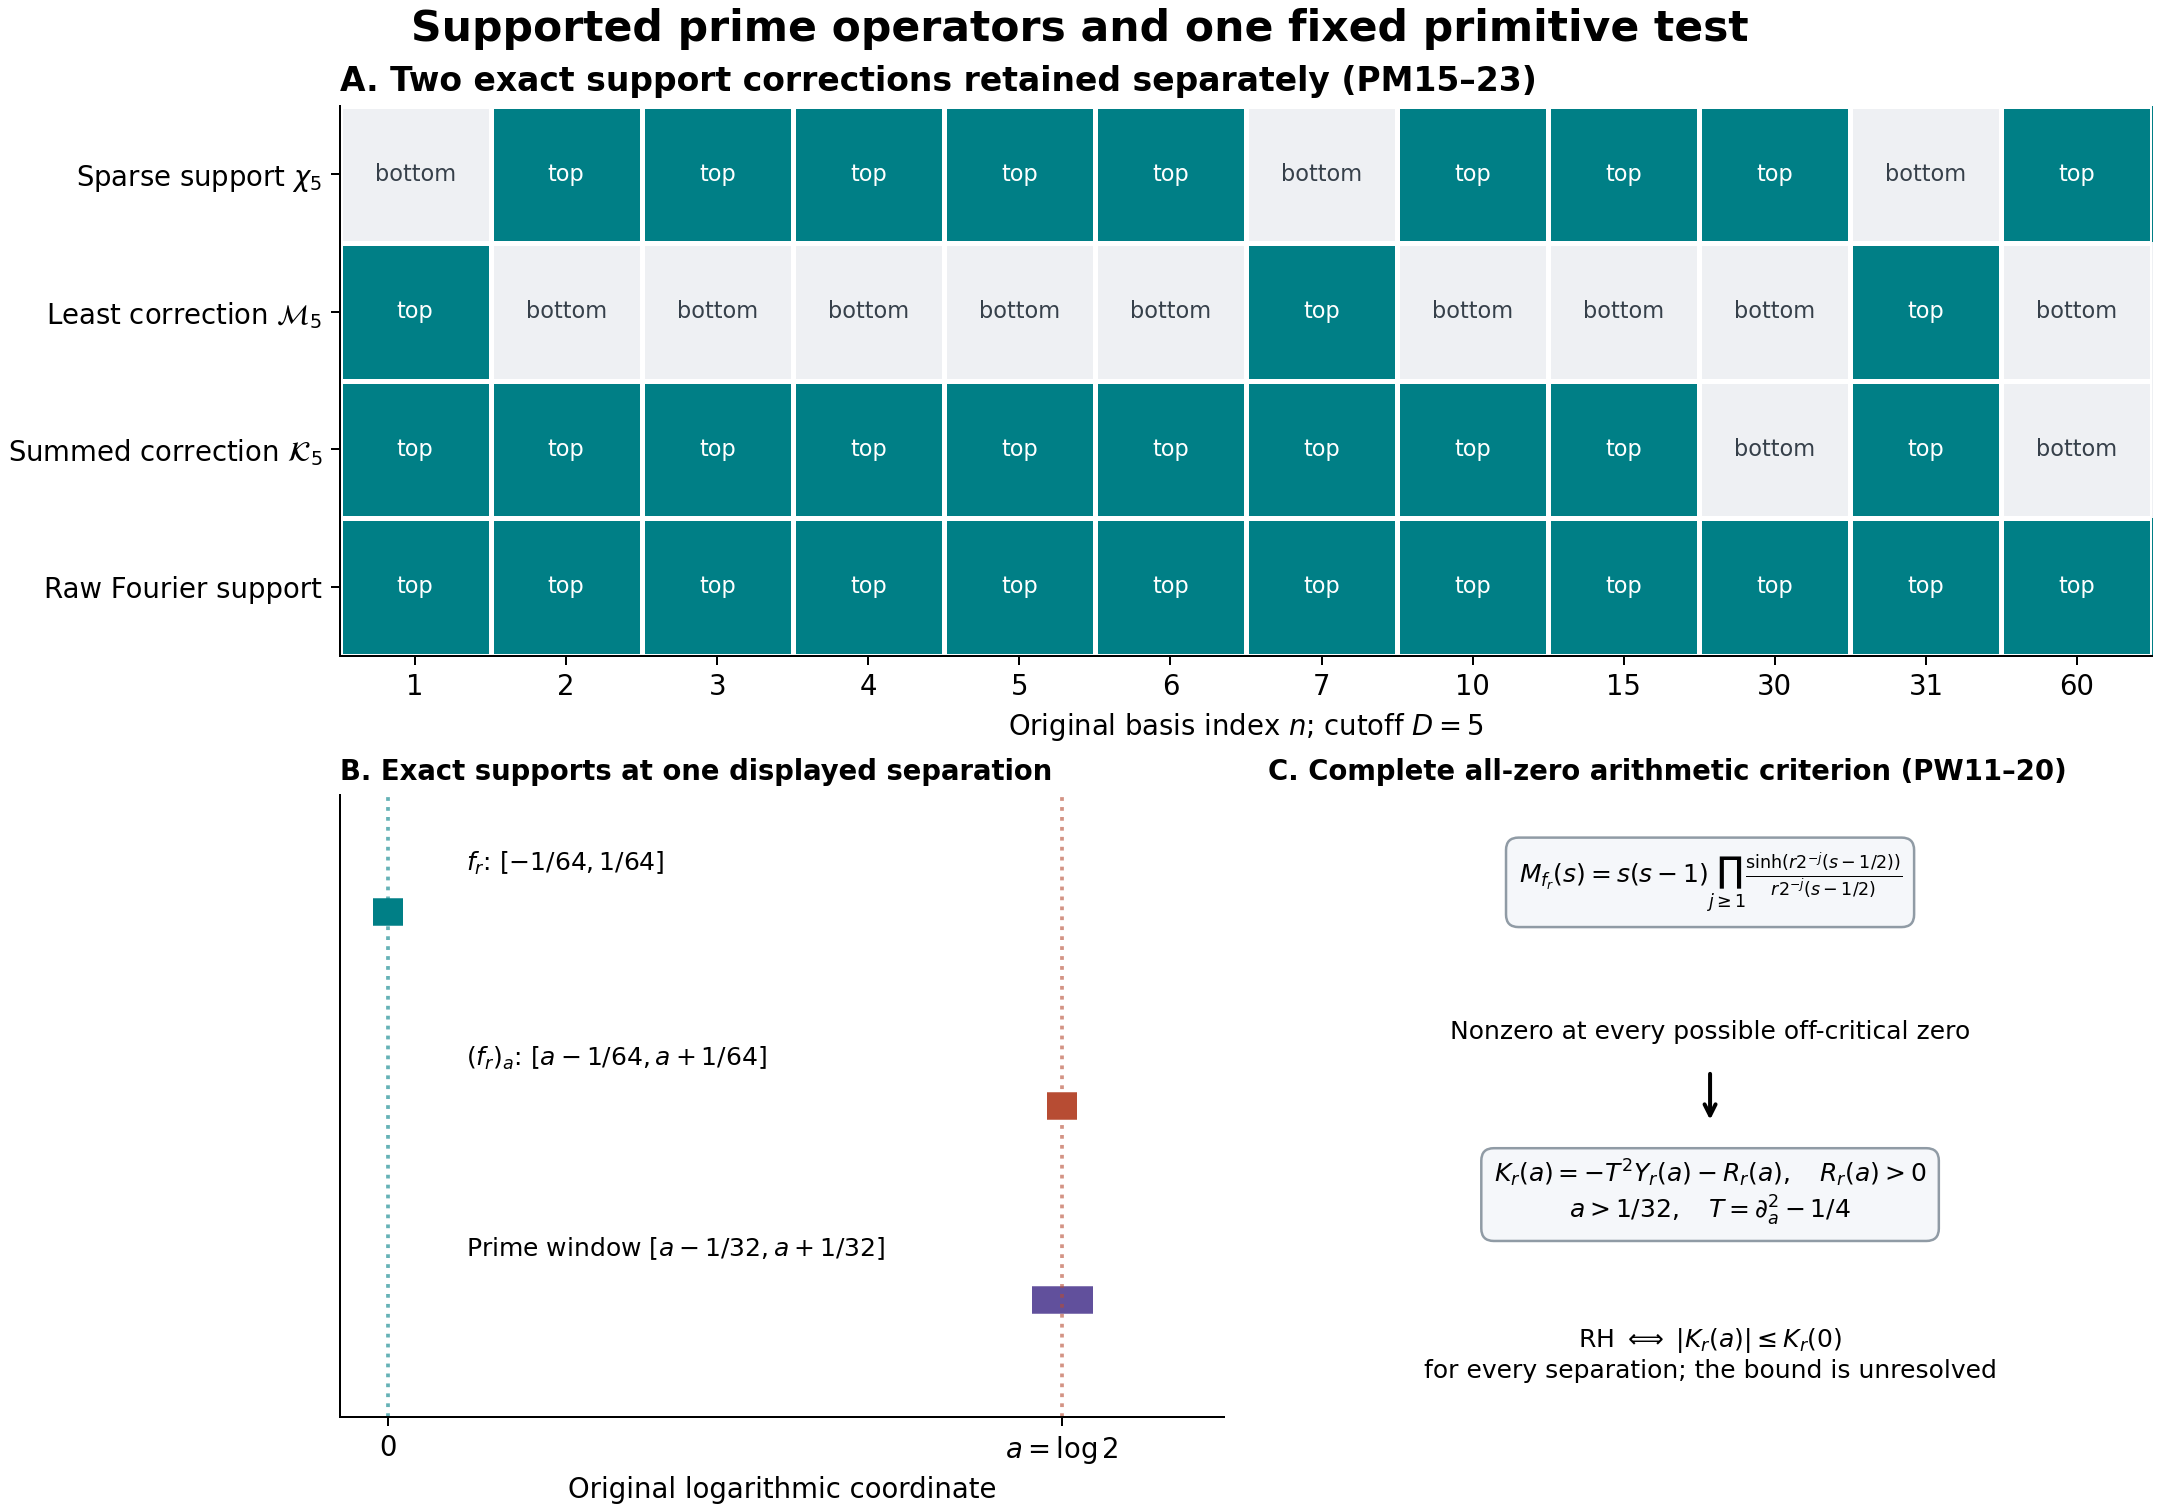
\includegraphics[keepaspectratio,alt={Exact support masks at cutoff five, the original test-support intervals and their prime window, and the complete criterion. The top panel shows all labels at the displayed indices, including the difference between the least correction and the directly summed Fourier correction. The middle support calculation uses the displayed separation a=log 2; the criterion concerns every separation. Proofs: PM15--23 and PW3--20. Both zero endpoint values retain supported-zero labels by PW21--22. The reproducible source draws the proved masks and interval coordinates; it does not sample a hypothetical zero.}]{primitive_prime_window.png}}
\caption{Exact support masks at cutoff five, the original test-support
intervals and their prime window, and the complete criterion. The top
panel shows all labels at the displayed indices, including the
difference between the least correction and the directly summed Fourier
correction. The middle support calculation uses the displayed separation
a=log 2; the criterion concerns every separation. Proofs: PM15--23 and
PW3--20. Both zero endpoint values retain supported-zero labels by
PW21--22. The reproducible source draws the proved masks and interval
coordinates; it does not sample a hypothetical zero.}
\end{figure}

\subsection{Proof sources and scope}\label{proof-sources-and-scope}

The analytic explicit formula and full support vector are the complete
SZW source cited above; the Gamma integral is HA13. Their original human
source includes Alain Connes,
\href{https://arxiv.org/abs/math/9811068}{\emph{Trace formula in
noncommutative geometry and the zeros of the Riemann zeta function}},
Appendix II, Theorem 6. The incoming BPZ proof supplies the
translation/Laplace method with all multiplicities; its full TeX is
included unchanged. The present fixed convolution, its complete analytic
construction, the short-support estimate, and PM's prime-operator
comparison have standalone proofs in this collection. These statements
specify their exact mathematical contribution without claiming priority
over the extensive classical literature on Weil criteria or smoothed
prime formulas.

\subsection{Actual positive-real-time
continuation}\label{actual-positive-real-time-continuation-4}

The complete \href{REAL_TIME_HEAT_TRACE_DERIVATION.md}{real-time proof},
RT1--30, strengthens the compact-test variation in this edition: the
whole zero trace is smooth for the original real heat time t at least
zero, with actual right derivatives at zero. RT16 identifies its first
derivative with the full causal arithmetic distribution, and RT20--27
constructs every higher meromorphic derivative receiver. The contact
comparison retains the unit and inter-zero terms. These results do not
assert a common zero strip for negative or complex time and do not prove
the remaining RH inequality. All original supported carriers remain
present.

\subsection{Proved compact-interval and finite-translation
bounds}\label{proved-compact-interval-and-finite-translation-bounds-2}

The complete \href{FIRST_PRIME_FULL_WEIL_COERCIVITY.md}{compact-interval
proof}, FC1--43, proves full Weil coercivity with constant 11509/600000
through support diameter 19/25, including prime 2 and both original
endpoint moments. \href{FIRST_PRIME_WINDOW_BOUND.md}{FW1--21} proves the
every-rank matrix bound for centre diameter 583/800 and a strict
two-test margin through the next prime gap. The same unchanged test now
satisfies its required strict correlation bound for every positive
translation through log 256, by
\href{FINITE_PRIME_WINDOW_EXTENSION.md}{FP1--25} and the complete
\href{FINITE_PRIME_WINDOW_COEFFICIENT_CERTIFICATE.md}{rational
prime-power certificate, FPC1--14}.
\href{PRIME_TWO_HEAT_TAIL_DERIVATION.md}{PT1--40} calculates the
surviving mixed channel and proves a strictly negative full actual right
heat derivative on the stated short interval after the prime-2 atom
ends. These are exact portions of the original bound, retaining
supported zero and every original arithmetic coefficient. The uniform
inequality beyond log 256 remains unproved.

\subsection{Original-zeta Gaussian and affine receiving
maps}\label{original-zeta-gaussian-and-affine-receiving-maps-2}

The complete extension OZG1--55 proves that Gaussian convolution of the
test at every positive time makes the original trivial-zero scalar sum
diverge for every real translation. Its admissible replacement retains
each cutoff trace and the Gamma boundary with the identical finite sum
U\_N; OZG20--27 gives both maps and the inverse. The full coefficient
tower, its raw non-Hermitian correction and exact compensated negative
index are OZG28--39. No compact-support prime window is assumed after
smoothing; all prime powers and Gamma terms, with explicit error bounds,
are OZG40--52. This extension acts on the tests while fixing the
original zeta zeros.

The different affine change of the actual original heat family is
OZR1--36. Its multiplier is exp(chi) C(phi)/C, with the full inverse,
exceptional units and local jets. The original generator contains every
q derivative term. The signed divisor comparison is OZR19--24; its
Cauchy logarithmic kernel has an additional growth contribution 2a.
OZR33 proves the exact full negative index after that contribution is
retained. The full support carrier and every lower coordinate are
OZG53--55 and OZR34--36. These are the receiving maps for these
specified extensions; the original preceding test, time and domains
remain those stated in its proof.

\clearpage

\section{Global contact variation on the fixed primitive
test}\label{global-contact-variation-on-the-fixed-primitive-test}

\textbf{Original-zeta receiving calculation.} The working meromorphic
function is the original Riemann zeta, with its full Gamma/endpoints
multiplier and its full trivial-zero and pole divisor retained.
\href{FAITHFUL_THETA_COMPLETION_RETURN.md}{TF1--42} proves the original
labelled theta inverse and the actual heat-image defect.
\href{FAITHFUL_UNCOMPLETED_ZETA_HEAT.md}{UZ1--53} proves every
exceptional-point fibre, jet, original-zeta heat term and reflection
orientation.
\href{ORIGINAL_ZETA_COMPACT_WEIL_RECONSTRUCTION.md}{OZC1--48} rederives
the compact contour and interval operator directly from zeta, including
the left-cutoff Gamma boundary, and specifies exactly which compensated
pairing the bounds concern.
\href{ORIGINAL_ZETA_HEAT_CONTACT_RECONSTRUCTION.md}{OZH1--49} rederives
the actual meromorphic heat, rational signed trace, compact-test domain,
contact drift and full causal arithmetic variation. The raw full divisor
and the compensated Weil receiver are linked by their displayed
correction, not identified. In particular the fixed-test trivial-zero
sum converges exactly at translations at least 1/32 and equals the
earlier R term; at zero translation it requires the proved cutoff
compensation. \href{ORIGINAL_ZETA_CAUCHY_RECONSTRUCTION.md}{OZK1--38}
reconstructs the original signed Cauchy trace, its full Gamma
correction, resonant finite parts, every finite matrix and its index,
and the complete local heat jets. Its invertible map retains the raw
trace and correction separately. These complete receiving proofs govern
the interpretation of the retained auxiliary calculations below.

This proof evaluates the complete contact contribution on the single
fixed primitive test, proves its global convergence, and computes its
exact meromorphic Laplace receiver. It then combines that contribution
with the regularized variation of the genuine heat family. The surviving
terms retain every analytic unit and every interaction between distinct
zeros. Adding this scalar contact contribution is not asserted to
construct a new global heat family.

The sources used are
\href{ACTUAL_HEAT_ZERO_DISTRIBUTION_VARIATION.md}{AG17--AG24},
\href{UNIVERSAL_PRIMITIVE_TRANSLATION_CRITERION.md}{UP1--UP35}, and the
complete companion proof
\href{CONTACT_DEFECT_TRACE_VARIATION.tex}{BT1--BT22}. The last source is
retained at its original programme path in the source-use record. The
arithmetic coordinate and the factor \(1/4\) below are exactly those of
AG1 and BT13--BT18.

\subsection{1. Original objects and the fixed family of
tests}\label{original-objects-and-the-fixed-family-of-tests}

Let \[
g_t(s)=16H_t(-2i(s-\tfrac12)),\qquad g_0=2\xi_R,\qquad
\partial_tg_t=\tfrac14\partial_s^2g_t.
\tag{GC1}
\] Let \(\mathcal Z\) be the set of distinct zeros of \(g_0\), with
multiplicities \(m_\rho\), and retain the local factorization \[
g_0(s)=(s-\rho)^{m_\rho}u_\rho(s),\qquad
u_\rho(\rho)\ne0,\qquad
b_\rho=\frac{u_\rho'(\rho)}{u_\rho(\rho)},\qquad
c_\rho=\rho-\tfrac12.
\tag{GC2}
\] The symbols \(b_\rho\) are the complete local-unit logarithmic
derivatives, not free parameters. In particular, their expression in
terms of the other zeros will be retained below.

Use the fixed density \(b_r\) of UP1--UP11, with \(r=1/64\), and put \[
\begin{gathered}
f_r=(\partial_v^2-\tfrac14)b_r,\qquad
F(s)=M_{f_r}(s)=s(s-1)G_r(s-\tfrac12),\\
H(s)=F(s)^2,\qquad A_a(s)=e^{a(s-1/2)}H(s)
\quad(a\in\mathbb R).
\end{gathered}
\tag{GC3}
\] Here \(H(s)\) denotes the square of the fixed Mellin test, and is
distinct from the original heat function \(H_t(Z)\). The product theorem
UP11 gives \(F(\rho)\ne0\) at every actual off-critical zero. We do not
assert this nonvanishing at every critical zero.

Every derivative \(F^{(j)}\) decreases faster than any inverse power of
height on each fixed closed vertical strip. Indeed, \[
F^{(j)}(s)=\int_{\mathbb R}(-v)^jf_r(v)e^{-(s-1/2)v}\,dv,
\] and \((-v)^jf_r(v)\) is compactly supported and smooth. Repeated
integration by parts in its Fourier factor proves the claim, uniformly
in the real part on the strip. Products and derivatives therefore give
the same assertion for \(H\).

For every fixed pair of nonnegative integers \(k,N\), there is a finite
constant \(C_{k,N}\) such that, for \(a\ge0\), \[
\max_{0\le j\le2}\sup_{0\le\Re s\le1}
(1+|\Im s|)^N
\left|\partial_s^j\partial_a^k A_a(s)\right|
\le C_{k,N}(1+a^2)e^{a/2}.
\tag{GC4}
\] To prove this, \(\partial_a^kA_a=(s-1/2)^ke^{a(s-1/2)}H(s)\). Taking
at most two spatial derivatives introduces at most \(a^2\), fixed powers
of \(s-1/2\), and derivatives of \(H\) of order at most two. The
preceding rapid decrease absorbs those powers; the exponential has
modulus at most \(e^{a/2}\) on the strip. For \(a\) in a bounded
interval of the whole real line, the same proof gives a uniform bound,
with \(e^{|a|/2}\) in place of \(e^{a/2}\).

\subsection{2. The global contact sum and all real
derivatives}\label{the-global-contact-sum-and-all-real-derivatives}

BT15 assigns the contribution \(m_\rho(m_\rho-1)A''(\rho)/4\) at an
actual centre. Define the full scalar receiver \[
\mathcal C(a)=\frac14\sum_{\rho\in\mathcal Z}
m_\rho(m_\rho-1)A_a''(\rho).
\tag{GC5}
\] The sum converges absolutely, uniformly for \(a\) in every compact
real interval, and remains so after every number of real
\(a\)-derivatives.

For a detailed bound, AG4 gives a constant with total multiplicity at
modulus at most \(R\) bounded by \(C R\log(R+2)\). On a dyadic annulus
of radius \(R\), therefore, \[
\sum_{\rho\ {\rm in\ annulus}}m_\rho(m_\rho-1)
\le\left(\sum_{\rho\ {\rm in\ annulus}}m_\rho\right)^2
=O(R^2\log^2(R+2)).
\tag{GC6}
\] On the strip, modulus and height are comparable outside a fixed disc.
Equations (GC4) and (GC6), with any sufficiently large \(N\), bound the
sum of absolute values on this annulus by
\(C_{k,N}(1+a^2)e^{a/2}R^{2-N}\log^2(R+2)\). Summing the dyadic annuli
proves both the stated normal convergence and \[
\mathcal C\in C^\infty(\mathbb R),\qquad
\mathcal C^{(k)}(a)=
\frac14\sum_\rho m_\rho(m_\rho-1)
\partial_s^2\!\left((s-\tfrac12)^k A_a(s)\right)_{s=\rho},
\quad
|\mathcal C^{(k)}(a)|\le C_k(1+a^2)e^{a/2}
\quad(a\ge0).
\tag{GC7}
\] Termwise differentiation follows from uniform convergence on real
compact intervals at each order. Thus (GC5) is a defined contribution on
the full actual zero multiset; no omitted tail or bound on individual
multiplicities is assumed.

The exact summand is \[
A_a''(\rho)=e^{ac_\rho}
\left(a^2F(\rho)^2+4aF(\rho)F'(\rho)
+2F'(\rho)^2+2F(\rho)F''(\rho)\right).
\tag{GC8}
\] This follows from \(H'=2FF'\) and \(H''=2(F')^2+2FF''\). All
derivatives are taken in the original coordinate \(s\). The function
\(\mathcal C\) is real and even on the real axis: conjugation of the
zero set gives reality, while reflection \(\rho\mapsto1-\rho\), with its
unchanged multiplicity, gives \(A_a''(1-\rho)=A_{-a}''(\rho)\). These
changes of summation variable are justified by the absolute convergence
just proved.

\subsection{3. Exact contact Laplace
poles}\label{exact-contact-laplace-poles}

For \(\Re w>1/2\), define \[
\Psi_w(s)=\frac{H(s)}{w-(s-1/2)}.
\tag{GC9}
\] The original strip is free of the test pole at \(s=w+1/2\). Fubini's
theorem, justified by (GC6)--(GC7) and the exponential margin
\(\Re w-1/2>0\), gives \[
\widehat{\mathcal C}(w)
:=\int_0^\infty e^{-wa}\mathcal C(a)\,da
=\frac14\sum_\rho m_\rho(m_\rho-1)\Psi_w''(\rho).
\tag{GC10}
\] For example, integrating the absolute majorant in (GC4) multiplies
the convergent annular bound by
\(\int_0^\infty(1+a^2)e^{-(\Re w-1/2)a}da<\infty\). Writing
\(p_\rho=w-c_\rho\), direct differentiation in \(s\) gives \[
\widehat{\mathcal C}(w)=
\sum_\rho\frac{m_\rho(m_\rho-1)}4
\left(
\frac{2H(\rho)}{p_\rho^3}
+\frac{2H'(\rho)}{p_\rho^2}
+\frac{H''(\rho)}{p_\rho}
\right).
\tag{GC11}
\] The sign of every denominator derivative is positive because
\(\partial_s(w-(s-1/2))=-1\).

The series in (GC11) extends meromorphically to the whole \(w\)-plane.
On a compact set avoiding the discrete points \(c_\rho\), its finitely
many bounded-height terms have separated denominators, and all
sufficiently high terms have \(|p_\rho|\ge|\Im\rho|/2\). The rapid
decrease of \(H,H',H''\) and (GC6) make the tail uniformly absolutely
summable. The same argument applies in a small disc around one
\(c_\rho\) after that one term is removed. Its complete principal part
is consequently \[
\boxed{
\operatorname{PP}_{c_\rho}\widehat{\mathcal C}
=
\frac{m_\rho(m_\rho-1)F(\rho)^2}{2(w-c_\rho)^3}
+\frac{m_\rho(m_\rho-1)F(\rho)F'(\rho)}{(w-c_\rho)^2}
+\frac{m_\rho(m_\rho-1)
\bigl(F'(\rho)^2+F(\rho)F''(\rho)\bigr)}
{2(w-c_\rho)}.}
\tag{GC12}
\] Thus each off-critical multiple zero has a nonzero triple pole in
this receiver, because \(m_\rho(m_\rho-1)>0\) and \(F(\rho)\ne0\). Each
simple zero is absent from this contact receiver. At a critical zero,
(GC12) states every possible cancellation through the actual values
\(F,F',F''\); none of these values is discarded.

\subsection{4. The genuine heat variation and the exact residual
term}\label{the-genuine-heat-variation-and-the-exact-residual-term}

Set \(b=g_0'(0)/g_0(0)\), and for distinct zeros define, as in AG19, \[
T_A(\rho,\eta)=
\frac{A'(\rho)-A'(\eta)}{\rho-\eta}
+\frac{A'(\rho)}{\eta}+\frac{A'(\eta)}{\rho}.
\tag{GC13}
\] The regularized genuine-heat variation is precisely AG20 and AG22: \[
\begin{aligned}
\mathcal V(a):=\mathcal V(A_a)
=-\frac14\Bigg[&
\sum_\rho m_\rho(m_\rho-1)A_a''(\rho)
+2b\sum_\rho m_\rho A_a'(\rho)\\
&+2\sum_\rho\frac{m_\rho^2 A_a'(\rho)}{\rho}
+2\sum_{\{\rho,\eta\}}m_\rho m_\eta T_{A_a}(\rho,\eta)
\Bigg].
\end{aligned}
\tag{GC14}
\] The last sum is over unordered pairs of distinct supports. Define the
residual scalar after adding the contact contribution: \[
\boxed{
\begin{aligned}
\mathcal R(a):=\mathcal V(a)+\mathcal C(a)
=-\frac12\Bigg[
b\sum_\rho m_\rho A_a'(\rho)
+\sum_\rho\frac{m_\rho^2 A_a'(\rho)}{\rho}
+\sum_{\{\rho,\eta\}}m_\rho m_\eta T_{A_a}(\rho,\eta)
\Bigg].
\end{aligned}}
\tag{GC15}
\] This cancels exactly the second-derivative summand, with its factor
\(1/4\), and no other term. Formula (GC15), including its grouped pair
term, is the global definition of the residual. It does not assume that
the ungrouped series \(\sum m_\rho b_\rho A_a'(\rho)\) is absolutely
convergent.

Here are bounds that justify the complete real-parameter statement. The
absolute-convergence proof of AG19--AG21 is uniform on any bounded set
of the rapid-decay seminorms in AG18. Explicitly, for comparable large
\(|\rho|\le|\eta|<2|\rho|\), either their separation is at least
\(|\rho|/2\), so endpoint values bound the divided difference, or the
segment joining them stays at modulus at least \(|\rho|/2\); integration
of \(A''\) along that segment then bounds it. Both cases give
\(C_N(1+|\rho|)^{-N}\) times the seminorm of \(A\). The multiplicity sum
on a comparable dyadic pair annulus is \(O(R^2\log^2(R+2))\).

For \(|\eta|\ge2|\rho|\), retain the cancellation \[
T_A(\rho,\eta)=
\frac{\rho A'(\rho)}{\eta(\rho-\eta)}
+\frac{\eta A'(\eta)}{\rho(\eta-\rho)}.
\tag{GC16}
\] Its absolute value is at most
\(2|\rho||A'(\rho)|/|\eta|^2+2|A'(\eta)|/|\rho|\). AG's zero count gives
\(\sum_{|\eta|\ge R}m_\eta/|\eta|^2=O(\log(R+2)/(R+1))\) and
\(\sum_{|\rho|\le R}m_\rho/|\rho|=O(\log^2(R+2))\). These bounds prove
summability of the two disparate-pair terms, uniformly in the same
seminorms. The finitely many small zeros have nonzero denominators,
since \(g_0(0)\ne0\).

Applying these explicit estimates to (GC4) proves absolute convergence
of every single and grouped pair sum in (GC14)--(GC15), locally
uniformly in real \(a\), together with every real derivative. It also
proves \[
\mathcal V,\mathcal R\in C^\infty(\mathbb R),\qquad
|\mathcal V^{(k)}(a)|+|\mathcal R^{(k)}(a)|
\le C_k(1+a^2)e^{a/2}\quad(a\ge0).
\tag{GC17}
\] The derivatives are obtained by replacing \(A_a\) by \((s-1/2)^kA_a\)
in the formulas. This is a global statement about the exactly specified
AG regularized variation. It does not replace that regularization by an
unproved derivative of a global moving-zero sum for arbitrary entire
tests.

\subsection{5. Meromorphic receiver of the retained unit and pair
interactions}\label{meromorphic-receiver-of-the-retained-unit-and-pair-interactions}

For \(\Re w>1/2\), the estimates just proved permit taking Laplace
transforms through every \textbf{grouped} sum in (GC14)--(GC15). Indeed
their integrable majorant is a constant times
\((1+a^2)e^{-(\Re w-1/2)a}\). Thus \[
\begin{aligned}
\widehat{\mathcal V}(w)&=\mathcal V(\Psi_w),\\
\widehat{\mathcal R}(w)&=
-\frac12\left[
b\sum_\rho m_\rho\Psi_w'(\rho)
+\sum_\rho\frac{m_\rho^2\Psi_w'(\rho)}{\rho}
+\sum_{\{\rho,\eta\}}m_\rho m_\eta T_{\Psi_w}(\rho,\eta)
\right],\\
\widehat{\mathcal V}(w)+\widehat{\mathcal C}(w)
&=\widehat{\mathcal R}(w).
\end{aligned}
\tag{GC18}
\] On this half-plane \(\Psi_w\) is holomorphic on the entire zero strip
and satisfies the rapid-decrease estimates used in AG. The notation
\(\mathcal V(\Psi_w)\) in (GC18) means the explicit grouped expression
(GC14) evaluated on this test; that expression is well defined by those
strip estimates, although \(\Psi_w\) has its stated pole outside the
strip.

The displayed expressions extend meromorphically to every
\(w\in\mathbb C\), with possible poles only at \(c_\rho\). This
assertion retains the grouped pair series. To prove it, fix a compact
\(w\)-set with \(|w|\le M\) avoiding those points. For sufficiently high
spatial points in the original strip, \(|w-(s-1/2)|\ge |s|/2\). The
functions \(\Psi_w'\) and \(\Psi_w''\) therefore have rapid-decay bounds
there uniformly in \(w\).

For pairs at comparable high moduli, the proof preceding (GC16) applies
uniformly: if a connecting segment is needed, it remains at large
modulus and hence avoids the moving test pole \(s=w+1/2\). For
well-separated comparable pairs, only endpoint values are used. For
disparate pairs use the exact formula (GC16); finitely many
bounded-height values and the high-height estimates supply its required
bounds. Pairs with both heights bounded form a finite set and are
meromorphic in \(w\), with no pole on the chosen compact set. The
resulting absolute normal convergence proves the extension away from the
discrete points.

To compute its principal part at \(c_\rho\), isolate every pair
containing that one zero. The coefficient of \(\Psi_w'(\rho)\) in the
bracket in (GC18) is \[
m_\rho\left[
b+\frac{m_\rho}{\rho}
+\sum_{\eta\ne\rho}m_\eta
\left(\frac1{\rho-\eta}+\frac1\eta\right)
\right]=m_\rho b_\rho.
\tag{GC19}
\] This is exactly AG23. The inner series is absolutely convergent for
this fixed \(\rho\), by its genus-one cancellation: its high-height
summand is \(O_\rho(m_\eta/|\eta|^2)\). The other terms of those pairs
multiply \(\Psi_w'(\eta)\) and are holomorphic near \(c_\rho\); their
normal convergence there follows from the rapid decrease at \(\eta\).
The pairs not containing \(\rho\) also converge normally there by the
preceding argument. Consequently \[
\boxed{
\operatorname{PP}_{c_\rho}\widehat{\mathcal R}
=-\frac{m_\rho b_\rho}{2}
\left[
\frac{H(\rho)}{(w-c_\rho)^2}
+\frac{H'(\rho)}{w-c_\rho}
\right].}
\tag{GC20}
\] In the original fixed-test values, \(H=F^2\) and \(H'=2FF'\). Thus
the complete genuine-heat receiver has principal part \[
\boxed{
\operatorname{PP}_{c_\rho}\widehat{\mathcal V}
=-\operatorname{PP}_{c_\rho}\widehat{\mathcal C}
-\frac{m_\rho b_\rho}{2}
\left[
\frac{F(\rho)^2}{(w-c_\rho)^2}
+\frac{2F(\rho)F'(\rho)}{w-c_\rho}
\right].}
\tag{GC21}
\] These identities compute the exact cancellation and the entire
remaining local principal part. They do not suppress the inter-zero
interactions: (GC19) is the map carrying them into the actual local unit
\(b_\rho\).

At an off-critical multiple zero, the genuine variation has a nonzero
triple pole with the negative of the coefficient in (GC12). The added
contact term removes that triple pole. The residual still has a double
pole precisely when \(b_\rho\ne0\), since \(F(\rho)\ne0\). At an
off-critical simple zero, \(\widehat{\mathcal C}\) is holomorphic and
(GC20) is the whole first variation. It has a nonzero double pole
exactly when \(b_\rho\ne0\); if \(b_\rho=0\), both its displayed
coefficients vanish. This computation does not assert that the actual
simple-zero unit derivatives are all nonzero.

\subsection{6. Exact map from the full translation resolvent to its heat
variation}\label{exact-map-from-the-full-translation-resolvent-to-its-heat-variation}

The original time-zero kernel and its Laplace transform are UP20 and
UP23: \[
K_r(a)=\sum_\rho m_\rho H(\rho)e^{ac_\rho},\qquad
\mathscr K_r(w)=\sum_\rho\frac{m_\rho H(\rho)}{w-c_\rho}.
\tag{GC22}
\] Their residue at \(c_\rho\) is \(m_\rho F(\rho)^2\). In particular it
is nonzero at every actual off-critical zero, including a simple zero
with \(b_\rho=0\). The absence of such a zero from the \textbf{first
variation} is not its absence from this original resolvent.

We specify exactly the derivative map in (GC18). Take the separated
rectangular contours \(\Gamma_j\) of AG22, with real edges \(-1,2\). For
each fixed \(j\), the actual function \(L_t=g_t'/g_t\) is holomorphic on
the contour for a sufficiently small complex time disc. For
\(\Re w>3/2\), the point \(w+1/2\) lies to the right of the contour.
Define \[
\mathscr K_{r,j}(t,w)
=\frac1{2\pi i}\int_{\Gamma_j}\Psi_w(s)L_t(s)\,ds.
\tag{GC23}
\] This is the sum of the actual zero-cluster residues inside that
contour, including all multiplicities, and is holomorphic in time on the
stated local disc. At time zero its limit as \(j\to\infty\) is
\(\mathscr K_r(w)\), by absolute convergence of (GC22). The residue
proof of AG22 extends to this test with its pole outside the contours,
as justified immediately below, and gives \[
\widehat{\mathcal V}(w)
=\lim_{j\to\infty}
\left.\partial_t\mathscr K_{r,j}(t,w)\right|_{t=0}
\qquad(\Re w>3/2).
\tag{GC24}
\] The test \(\Psi_w\) is holomorphic on and inside these contours, and
its rapid strip bounds used in AG's proof hold on the slightly wider
strip as well; they follow from the fixed compact support of \(f_r\).
The residue derivation and cross-boundary estimates AG23--AG24 therefore
apply without a test-pole correction in this specified half-plane.

For a test pole \(p=w+1/2\) strictly inside a particular contour and not
a zero or a point on the contour, the precise finite correction is also
explicit: \[
\sum_{\rho_t\ {\rm inside}\ \Gamma_j}
m_{\rho_t}\Psi_w(\rho_t)
=\frac1{2\pi i}\int_{\Gamma_j}\Psi_w L_t\,ds
+H(p)L_t(p).
\tag{GC25}
\] The added term follows because
\(\operatorname{Res}_{s=p}\Psi_w(s)=-H(p)\). On a time disc where \(p\)
stays a nonzero point and the contour stays zero-free, this equality may
be differentiated, with the correction differentiated too. Equation
(GC24), first proved where the pole is outside, and the unique
meromorphic continuation in (GC18) specify the complete regularized
derivative receiver. No test pole is silently moved through a contour.

Equations (GC18), (GC22), and (GC24) are the promised map to the full
original \(K_r\) Laplace transform: apply the actual heat derivative at
each fixed zero-isolating exhaustion, then take the proven regularized
limit. They do not claim interchange of the infinite zero limit and the
time derivative on the entire moving-zero family. Nor do they claim that
\(\mathcal R\), obtained by adding the contact term, is the derivative
of a globally constructed persistent-contact family.

\subsection{7. A stationary first derivative does not imply a stationary
simple
zero}\label{a-stationary-first-derivative-does-not-imply-a-stationary-simple-zero}

There is a further exact local statement about the genuine heat family.
No fixed complex spatial point \(s\) is a zero of \(g_t(s)\) for every
time. Indeed the original integral gives, for \(T>0\), \[
g_{-T}(s)=16\int_0^\infty
e^{-Tu^2}\Phi(u)\cosh(2(s-\tfrac12)u)\,du.
\tag{GC26}
\] The kernel \(\Phi\) is continuous and bounded on \([0,\infty)\), by
its defining series and its superexponential bound in AG2, and
\(\Phi(0)>0\), since every term there is positive. Substitute
\(x=\sqrt T\,u\). For \(T\ge1\) the resulting integrand is bounded in
modulus by \[
\|\Phi\|_\infty e^{-x^2}e^{2|\Re(s-1/2)|x},
\] an integrable function. Dominated convergence proves the exact limit
\[
\lim_{T\to\infty}\sqrt T\,g_{-T}(s)
=16\Phi(0)\int_0^\infty e^{-x^2}dx
=8\sqrt\pi\,\Phi(0)>0.
\tag{GC27}
\]

For an actual simple zero \(\rho\), joint holomorphy and
\(g_0'(\rho)\ne0\) give one analytic zero branch \(\rho(t)\) near zero
time and its complete nonvanishing unit. Since \(t\mapsto g_t(\rho)\) is
entire and is not identically zero by (GC27), define its finite first
nonvanishing order by \[
n_\rho=\min\{n\ge1:g_0^{(2n)}(\rho)\ne0\}<\infty.
\tag{GC28}
\] The equality of its derivatives with \(4^{-n}g_0^{(2n)}(\rho)\)
follows by repeated differentiation of (GC1). Analytic local division
gives \(g_t(s)=(s-\rho(t))U(t,s)\), with \(U(0,\rho)=g_0'(\rho)\).
Evaluating this identity at the fixed point \(\rho\) gives \[
\rho(t)=\rho-
\frac{g_0^{(2n_\rho)}(\rho)}
{4^{n_\rho}n_\rho!\,g_0'(\rho)}\,t^{n_\rho}
+O(t^{n_\rho+1}).
\tag{GC29}
\] This retains the original heat time; no reparameterization is used.

For the local weighted resolvent \(\Psi_w(\rho(t))\), all time
derivatives of order \(1,\ldots,n_\rho-1\) vanish. Its derivative at the
first nonzero motion order \(n_\rho\) is \[
\left.\partial_t^{n_\rho}\Psi_w(\rho(t))\right|_0
=-\frac{g_0^{(2n_\rho)}(\rho)}
{4^{n_\rho}g_0'(\rho)}
\left[
\frac{H(\rho)}{(w-c_\rho)^2}
+\frac{H'(\rho)}{w-c_\rho}
\right].
\tag{GC30}
\] This follows by Taylor substitution in (GC29); the factor \(n_\rho!\)
cancels exactly. At an off-critical simple zero its double-pole
coefficient is nonzero, since \(H(\rho)=F(\rho)^2\ne0\). For
\(n_\rho=1\), the identity \(g_0''(\rho)=2g_0'(\rho)b_\rho\) makes
(GC30) precisely (GC20) with \(m_\rho=1\). If the first-order unit drift
vanishes, a finite higher-order local receiver still detects the motion.

Equation (GC30) is proved for the actual finite zero cluster. It does
not assert convergence of the sum of these higher-order derivatives over
every zero. The global first-order receiver is (GC14)--(GC24); the
higher-order statement has the explicitly smaller local domain.

\subsection{8. Supported endpoints and interpretation of the
cancellation}\label{supported-endpoints-and-interpretation-of-the-cancellation}

The fixed tests satisfy \(F(0)=F(1)=0\), hence \(A_a(0)=A_a(1)=0\) for
every \(a\). All endpoint and lower fixed-support coordinates in the
original full explicit formula therefore have their evaluated zero
amplitudes. At the top spectral coordinate, the three scalar receivers
are \[
\boldsymbol{\mathcal V}(a)=\mathcal V(a)\mathbf e_{1_{\mathscr L}},
\qquad
\boldsymbol{\mathcal C}(a)=\mathcal C(a)\mathbf e_{1_{\mathscr L}},
\qquad
\boldsymbol{\mathcal R}(a)=\boldsymbol{\mathcal V}(a)
+\boldsymbol{\mathcal C}(a).
\tag{GC31}
\] The endpoint weights themselves have zero derivative for these fixed
tests. In the full identity
\(\boldsymbol B-\boldsymbol Z=\boldsymbol D\), the induced regularized
arithmetic coordinate, with the derivative-first order fixed in (GC24),
is therefore \[
\dot{\boldsymbol D}_{\rm reg}(a)
=-\mathcal V(a)\mathbf e_{1_{\mathscr L}},\qquad
\dot{\boldsymbol D}_{\rm reg,contact}(a)
-\dot{\boldsymbol D}_{\rm reg}(a)
=-\mathcal C(a)\mathbf e_{1_{\mathscr L}}.
\tag{GC31a}
\] All lower-coordinate amplitudes are zero. Thus the contact comparison
changes the spectral coordinate by \(+\mathcal C(a)\) and its
corresponding arithmetic coordinate by \(-\mathcal C(a)\). These are the
induced coordinates of the specified regularized identity. They are not
an independent differentiation of a prime expression at nonzero heat
time, nor a claim of a global moving-zero derivative for this entire
test. The definition of the original heat equation remains (GC1).

On the original synchronized supported carriers, each linear contour or
residue map retains its input label, as in BT22 and UP34--UP35. Thus a
zero scalar amplitude in (GC31) with top support remains the supported
zero \(e\), and not the unsupported element \(\tau\). The contact
classes are the full local BT6 classes, including their original
analytic units; their map to (GC5) is BT8--BT15 with the original
arithmetic coordinate. Their addition removes the multiple-zero
splitting term exactly, while (GC19)--(GC21) retains the unit and
inter-zero terms. None of these identities assigns positivity to the
complete original Weil form or implies RH.

\subsection{Source-use record}\label{source-use-record}

AG17--AG24 and their complete proofs were reread at the beginning of
this calculation. UP1--UP35 was verified at its previously reviewed
source version. BT1--BT22 and all proofs were read in full from:

\href{CONTACT_DEFECT_TRACE_VARIATION.tex}{Complete companion source,
BT1--22}

The original human heat source remains Brad Rodgers and Terence Tao, The
de Bruijn--Newman constant is non-negative, arXiv:1801.05914v5, with
exact author-source coordinates retained in AG and BT. This calculation
does not claim a fresh read of that author paper. The convergence,
meromorphic continuation, fixed-point asymptotic, and local higher-order
formulas needed here are proved above.

\subsection{Actual positive-real-time
continuation}\label{actual-positive-real-time-continuation-5}

The complete \href{REAL_TIME_HEAT_TRACE_DERIVATION.md}{real-time proof},
RT1--30, strengthens the compact-test variation in this edition: the
whole zero trace is smooth for the original real heat time t at least
zero, with actual right derivatives at zero. RT16 identifies its first
derivative with the full causal arithmetic distribution, and RT20--27
constructs every higher meromorphic derivative receiver. The contact
comparison retains the unit and inter-zero terms. These results do not
assert a common zero strip for negative or complex time and do not prove
the remaining RH inequality. All original supported carriers remain
present.

\clearpage

\section{The causal arithmetic distribution for the complete first heat
variation}\label{the-causal-arithmetic-distribution-for-the-complete-first-heat-variation}

\textbf{Original-zeta receiving calculation.} The working meromorphic
function is the original Riemann zeta, with its full Gamma/endpoints
multiplier and its full trivial-zero and pole divisor retained.
\href{FAITHFUL_THETA_COMPLETION_RETURN.md}{TF1--42} proves the original
labelled theta inverse and the actual heat-image defect.
\href{FAITHFUL_UNCOMPLETED_ZETA_HEAT.md}{UZ1--53} proves every
exceptional-point fibre, jet, original-zeta heat term and reflection
orientation.
\href{ORIGINAL_ZETA_COMPACT_WEIL_RECONSTRUCTION.md}{OZC1--48} rederives
the compact contour and interval operator directly from zeta, including
the left-cutoff Gamma boundary, and specifies exactly which compensated
pairing the bounds concern.
\href{ORIGINAL_ZETA_HEAT_CONTACT_RECONSTRUCTION.md}{OZH1--49} rederives
the actual meromorphic heat, rational signed trace, compact-test domain,
contact drift and full causal arithmetic variation. The raw full divisor
and the compensated Weil receiver are linked by their displayed
correction, not identified. In particular the fixed-test trivial-zero
sum converges exactly at translations at least 1/32 and equals the
earlier R term; at zero translation it requires the proved cutoff
compensation. \href{ORIGINAL_ZETA_CAUCHY_RECONSTRUCTION.md}{OZK1--38}
reconstructs the original signed Cauchy trace, its full Gamma
correction, resonant finite parts, every finite matrix and its index,
and the complete local heat jets. Its invertible map retains the raw
trace and correction separately. These complete receiving proofs govern
the interpretation of the retained auxiliary calculations below.

This calculation constructs a causal distribution whose pairing with
every original compact smooth Weil test equals the entire-test variation
AG20--24. The endpoint, Gamma, prime and mixed-prime terms all remain
explicit. The variation is the limit of derivatives of the stated finite
contour traces. No assertion that an unrestricted global moving-zero sum
of entire tests is differentiable is made.

\subsection{1. Original conventions and the inverse transform of the
full arithmetic
factor}\label{original-conventions-and-the-inverse-transform-of-the-full-arithmetic-factor}

Retain the heat family and coordinates of AG1 and HA1--4: \[
g_0(s)=2\xi_R(s),\qquad \partial_tg_t=\tfrac14g_t'',\qquad
L(s)=\frac{g_0'(s)}{g_0(s)},\qquad
J(s)=\left.\partial_t\frac{g_t'(s)}{g_t(s)}\right|_{t=0}
=\tfrac14\{L''(s)+2L(s)L'(s)\}.
\tag{CH1}
\] The equality follows by differentiating the quotient and using the
displayed heat equation; it retains the factor \(1/4\). The Mellin
convention is \[
M_h(s)=\int_{\mathbb R}h(v)e^{-(s-1/2)v}\,dv,
\qquad h\in C_c^\infty(\mathbb R;\mathbb C).
\tag{CH2}
\] All distributions below are distributions on the entire real line
with support in \([0,\infty)\). Their values at zero are distributional
values, not an implicit half-mass convention.

Write the original arithmetic decomposition on \(\Re s>1\) as \[
\begin{aligned}
a(s)&=\frac1s+\frac1{s-1}-\frac12\log\pi+\frac12\psi(s/2),\\
P(s)&=\sum_{n\ge2}\Lambda(n)n^{-s},\qquad L(s)=a(s)-P(s),\qquad
c_0=\frac{\gamma+\log\pi}{2}.
\end{aligned}
\tag{CH3}
\] Here \(\psi=\Gamma'/\Gamma\), \(\gamma\) is Euler's constant, and
\(\Lambda(n)=\log p\) for \(n=p^k\), otherwise zero, including
\(\Lambda(1)=0\). These are exactly HA10, not a changed prime norm.

Define \(\alpha\) by its complete test action: \[
\begin{aligned}
\langle\alpha,\varphi\rangle={}&
\int_0^\infty(e^{-v/2}+e^{v/2})\varphi(v)\,dv-c_0\varphi(0)\\
&+\int_0^\infty
\frac{e^{-2v}\varphi(0)-e^{-v/2}\varphi(v)}{1-e^{-2v}}\,dv,
\qquad\varphi\in C_c^\infty(\mathbb R).
\end{aligned}
\tag{CH4}
\] This specifies the subtraction at zero and the constant exactly.
Indeed its numerator at zero is
\(v(-3\varphi(0)/2-\varphi'(0))+O(v^2)\), while its denominator is
\(2v+O(v^2)\). The quotient is bounded near zero. Beyond the compact
support of \(\varphi\), its remaining numerator is
\(e^{-2v}\varphi(0)\), which is integrable. On a fixed compact test
support these estimates bound (CH4) by a constant times the supremum
norms of \(\varphi\) and \(\varphi'\). It is therefore a distribution of
order at most one. Its support is causal because every displayed value
or integral uses only \(v\ge0\).

For \(\Re s>1\), substitute \(\varphi(v)=e^{-(s-1/2)v}\) in the
convergent weighted action. The first integral gives \(1/s+1/(s-1)\). In
the second put \(x=2v\); its value is \[
\frac12\int_0^\infty\frac{e^{-x}-e^{-(s/2)x}}{1-e^{-x}}\,dx
=\frac12\{\psi(s/2)+\gamma\},
\tag{CH5}
\] by the original convergent digamma formula HA12. Thus \[
\boxed{M_\alpha(s):=\langle\alpha,e^{-(s-1/2)v}\rangle=a(s),\qquad\Re s>1.}
\tag{CH6}
\] The equality uses \(-c_0+\gamma/2=-\log\pi/2\); neither endpoint
denominator nor the Gamma constant is omitted.

\subsection{2. A derivative-of-measures presentation and all convolution
domains}\label{a-derivative-of-measures-presentation-and-all-convolution-domains}

To construct convolutions without multiplying the singular integrand in
(CH4) pointwise, set \[
g(v)=-\tfrac12e^{-v/2}\log(1-e^{-2v})\quad(v>0),\qquad
G=g(v)\mathbf1_{(0,\infty)}(v)\,dv,
\qquad
m=e^{v/2}\mathbf1_{(0,\infty)}(v)\,dv+\tfrac12G-c_0\delta_0.
\tag{CH7}
\] The function \(g\) is locally integrable: it is \(O(1+|\log v|)\)
near zero and \(O(e^{-5v/2})\) at infinity. It is positive for \(v>0\).
The exact distribution identity is \[
\boxed{\alpha=DG+m,}
\tag{CH8}
\] where \(D\) is the derivative on the whole real line, so
\(\langle DG,\varphi\rangle=-\int_0^\infty g(v)\varphi'(v)dv\).

Here is a direct verification retaining the singular boundary. For
\(v>0\), \[
g'(v)+\tfrac12g(v)=-\frac{e^{-5v/2}}{1-e^{-2v}},\qquad
\int_\varepsilon^\infty\frac{e^{-2v}}{1-e^{-2v}}dv
=-\tfrac12\log(1-e^{-2\varepsilon})=e^{\varepsilon/2}g(\varepsilon).
\tag{CH9}
\] Combine the \(e^{-v/2}\varphi(v)\) term of (CH4) with its subtracted
integral on \((\varepsilon,\infty)\), leaving \[
e^{\varepsilon/2}g(\varepsilon)\varphi(0)
-\int_\varepsilon^\infty\frac{e^{-5v/2}}{1-e^{-2v}}\varphi(v)dv.
\] Integration by parts in \(\langle(D+1/2)G,\varphi\rangle\) with the
same lower cutoff gives this expression with its first term replaced by
\(g(\varepsilon)\varphi(\varepsilon)\). The difference is
\(O(\varepsilon|\log\varepsilon|)\), which tends to zero. The discarded
short part of the regular \(e^{-v/2}\) integral also tends to zero. The
remaining \(e^{v/2}\) density and \(-c_0\delta_0\) are unchanged,
proving (CH8). Equations (CH4) and (CH8) are two proved presentations of
the same distribution; (CH4) continues to record the separate original
endpoint and Gamma inputs.

The prime measure and the full causal logarithmic derivative are \[
\pi=\sum_{n\ge2}\frac{\Lambda(n)}{\sqrt n}\delta_{\log n},
\qquad \nu=m-\pi,\qquad \ell=\alpha-\pi=DG+\nu.
\tag{CH10}
\] The measure \(\pi\) is locally finite, since there are finitely many
indices \(n\le e^R\) on any interval \([0,R]\). Every displayed measure
is a real signed measure, except that \(G\) and \(\pi\) individually are
nonnegative. For every \(c>1/2\), \[
\int_0^\infty e^{-cv}\,d|G|(v)<\infty,\qquad
\int_0^\infty e^{-cv}\,d|\nu|(v)<\infty.
\tag{CH11}
\] For \(\pi\), the integral is \(\sum\Lambda(n)n^{-c-1/2}<\infty\),
dominated by \(\sum(\log n)n^{-c-1/2}\). For the \(e^{v/2}\) density it
is \(1/(c-1/2)\); the remaining terms are already integrable after that
weight. Each of these weighted integrals remains finite with any fixed
polynomial in \(v\) inserted: reduce \(c\) by a small positive amount
while keeping it greater than \(1/2\), then absorb the polynomial into
that remaining exponential decay.

Convolution of the measures in (CH11) is defined by their product
measure and addition \((v,w)\mapsto v+w\). On the causal quadrant this
map is proper over each compact interval, so the convolution is locally
finite. Its weighted total variation is bounded by the product of the
two weighted total variations in (CH11), because
\(e^{-c(v+w)}=e^{-cv}e^{-cw}\). Derivatives of these convolutions give
the required distribution convolution. In particular its complete
definition here is \[
\ell*\ell=D^2(G*G)+2D(G*\nu)+\nu*\nu.
\tag{CH12}
\] For compact tests this also equals the distributional tensor product
action on \(\varphi(v+w)\), after inserting any smooth compact cutoff
equal to one on the part of the causal quadrant where \(v+w\) meets the
test support. Different such cutoffs have the same value, by the causal
supports. Thus (CH12) has the usual associativity, commutativity and
derivative identities, and does not depend on a singular pointwise
product. The corresponding formulas define \(\alpha*\alpha\),
\(\alpha*\pi\), and \(\pi*\pi\).

The transform of a causal derivative is \(M_{DU}(s)=(s-1/2)M_U(s)\).
This follows from the distributional derivative definition; the
exponential is justified by (CH11) and cutoff limits. Weighted Fubini
gives \(M_{U*V}=M_UM_V\) for these measures and hence their derivatives.
The same estimates, including the polynomial moments, justify
differentiation in \(s\), uniformly on compact subsets of \(\Re s>1\).
Therefore \[
M_\pi=P,\qquad M_\ell=L,\qquad
M_{vU}=-\partial_sM_U,\qquad
M_{\ell*\ell}=L^2\qquad(\Re s>1).
\tag{CH13}
\]

\subsection{3. The exact first-variation distribution and an explicit
compact test
formula}\label{the-exact-first-variation-distribution-and-an-explicit-compact-test-formula}

Define \[
\boxed{\mathfrak J=\tfrac14\{v^2\ell-v(\ell*\ell)\}.}
\tag{CH14}
\] Multiplication by \(v\) is multiplication of distributions by a
smooth function. This is a causal distribution of order at most two; it
has the exponential weighted bounds inherited from (CH11). For clarity,
multiplication of a derivative also admits a measure-derivative
presentation, for example \(vD^2U=D^2(vU)-2DU\) and
\(v^2DU=D(v^2U)-2vU\). Thus no uncontrolled order or growth is hidden by
(CH14). Its transform is exactly \[
\boxed{M_{\mathfrak J}(s)=\tfrac14\{L''(s)+(L(s)^2)'\}=J(s),\qquad\Re s>1.}
\tag{CH15}
\] Indeed \(M_{v^2\ell}=L''\) and \(M_{v(\ell*\ell)}=-(L^2)'\), fixing
the sign of the nonlinear term.

Every compact test pairing can be calculated without an undefined finite
part. In the following formula every symbol on an integral denotes an
ordinary locally finite measure from (CH7), (CH10), or their
convolution: \[
\begin{aligned}
4\langle\mathfrak J,F\rangle={}&
-\int_0^\infty(2vF(v)+v^2F'(v))\,dG(v)
+\int_0^\infty v^2F(v)\,d\nu(v)\\
&-\int_0^\infty(2F'(v)+vF''(v))\,d(G*G)(v)\\
&+2\int_0^\infty(F(v)+vF'(v))\,d(G*\nu)(v)
-\int_0^\infty vF(v)\,d(\nu*\nu)(v).
\end{aligned}
\tag{CH16}
\] It follows by substituting (CH10)--(CH12) into (CH14) and using the
distributional derivative definition twice. All these integrals are
finite for \(F\in C_c^\infty\), including at zero, by local finiteness
and the logarithmic integrability already proved. This provides an
explicit receiver with every subtraction and convolution justified.

\subsection{4. The regularized global zero variation equals the causal
receiver}\label{the-regularized-global-zero-variation-equals-the-causal-receiver}

Let \(h\in C_c^\infty(\mathbb R)\) and \(A=M_h\), using (CH2).
Integration by parts shows that \(A\), with each fixed number of its
derivatives, decreases faster than any inverse power of height,
uniformly on every fixed bounded real strip. In particular it satisfies
AG18, and also the stronger bounds on \(-1\le\Re s\le2\) needed below.

Use exactly AG22's separated heights \(T_j\in[j,j+1]\), at distance at
least \(j^{-3}\) from every \(|\Im\rho|\), and its positively oriented
rectangles \(\Gamma_j\) with real edges \(-1,2\). Each fixed contour has
an actual finite heat zero trace and an actual derivative at zero.
Differentiation on that fixed compact contour gives \[
\left.\frac d{dt}\right|_0\frac1{2\pi i}\int_{\Gamma_j}A(s)L_t(s)\,ds
=\frac1{2\pi i}\int_{\Gamma_j}A(s)J(s)\,ds.
\tag{CH17}
\] AG20--24 proves that the limit of the left side is its absolutely
convergent entire-test regularization \(\mathcal V(A)\). No interchange
with an unrestricted moving infinite zero sum has been made.

Here are the needed additional estimates to pass the right side to a
vertical line. The genus-one logarithmic derivative is \[
L(s)=b+\sum_\rho m_\rho\left((s-\rho)^{-1}+\rho^{-1}\right),
\quad L'(s)=-\sum_\rho m_\rho(s-\rho)^{-2},
\quad L''(s)=2\sum_\rho m_\rho(s-\rho)^{-3}.
\tag{CH18}
\] These derivative series converge normally off zeros by the zero count
and \(\sum m_\rho/|\rho|^2<\infty\). On the horizontal edges at
\(T=T_j\), the finitely many zeros with \(|\rho|\le3T+6\) are at
distance at least a fixed multiple of \(T^{-3}\). Their total
multiplicity is \(O(T\log T)\). Their contributions to \(L,L',L''\) are
consequently \(O(T^4\log T)\), \(O(T^7\log T)\), and
\(O(T^{10}\log T)\); the \(1/\rho\) sum is smaller, of size
\(O(\log^2T)\). In the remaining tails the paired summand of \(L\) is
\(s/[\rho(s-\rho)]\), giving \(O(\log T)\), and the two differentiated
tails are bounded by \(O(\log T/T)\) and \(O(\log T/T^2)\). Thus \[
\sup_{s\text{ on the horizontal edges}}|J(s)|
=O(T^{11}\log^2T).
\tag{CH19}
\] The rapid strip decay of \(A\) makes both horizontal integrals tend
to zero. On \(\Re s=2\), (CH11)--(CH16) give a polynomial bound for
\(J(2+it)\), of degree at most two, so its product with either
\(A(2+it)\) or \(A(-1-it)\) is absolutely integrable.

For every time, reflection gives \(L_t(1-s)=-L_t(s)\). Its derivative
gives \(J(1-s)=-J(s)\). Substituting \(s\mapsto1-s\) on the left
vertical edge, with its downward orientation retained, therefore proves
\[
\mathcal V(M_h)=\frac1{2\pi i}\int_{\Re s=2}
J(s)\{M_h(s)+M_h(1-s)\}\,ds.
\tag{CH20}
\] This uses the actual AG22 exhaustion; it is not an independently
imposed summation prescription.

The last step is Fourier inversion in the original convention. For any
of the exponentially bounded causal distributions used here and any
\(c>1\), \[
\begin{aligned}
\frac1{2\pi}\int_{\mathbb R}M_U(c+it)M_h(c+it)\,dt
&=\langle U,h(-v)\rangle,\\
\frac1{2\pi}\int_{\mathbb R}M_U(c+it)M_h(1-c-it)\,dt
&=\langle U,h(v)\rangle.
\end{aligned}
\tag{CH21}
\] To justify the formulas, first let \(U\) be a measure with finite
\(e^{-(c-1/2)v}\)-weighted total variation. Ordinary Fourier inversion
applied to the compact smooth weighted test and Fubini prove them. In
the first line the two integration variables satisfy \(u=-v\), and the
exponential weights cancel; in the second they satisfy \(u=v\), with the
opposite weights again cancelling. For a derivative of such a measure,
use the corresponding differentiated Fourier inversion formula and its
rapid decay. Distributional integration by parts gives the displayed
derivative pairing. Finite sums of such derivatives include
\(\mathfrak J\), by (CH16), with the polynomial moments justified in
(CH11). This proves both equalities with absolute convergence in the
Fourier variable.

Taking \(U=\mathfrak J\), (CH15), (CH20), and (CH21) give the closed
full receiver: \[
\boxed{\mathcal V(M_h)=\langle\mathfrak J,h(v)+h(-v)\rangle,
\qquad h\in C_c^\infty(\mathbb R).}
\tag{CH22}
\] Both the normalization and the evenized test on the right are forced
by the contour calculation. Equations (CH17)--(CH22) prove equality with
the AG regularization for the actual family. They do not identify that
regularization with a stronger global time derivative not established
for these entire tests.

\subsection{5. The full archimedean, prime and mixed-prime
expansion}\label{the-full-archimedean-prime-and-mixed-prime-expansion}

Expanding the actual \(\ell=\alpha-\pi\) in (CH14) yields \[
4\mathfrak J=
v^2\alpha-v(\alpha*\alpha)-v^2\pi
+2v(\alpha*\pi)-v(\pi*\pi).
\tag{CH23}
\] In particular let \(F(v)=h(v)+h(-v)\), and choose \(R\ge0\) with
\(\operatorname{supp}F\subset[-R,R]\). Its complete compact test formula
is \[
\begin{aligned}
4\mathcal V(M_h)={}&
\langle v^2\alpha-v(\alpha*\alpha),F\rangle\\
&-\sum_{2\le n\le e^R}\frac{\Lambda(n)}{\sqrt n}(\log n)^2F(\log n)\\
&+2\sum_{2\le n\le e^R}\frac{\Lambda(n)}{\sqrt n}
\left\langle\alpha,(v+\log n)F(v+\log n)\right\rangle\\
&-\sum_{2\le k\le e^R}\frac{(\Lambda*\Lambda)(k)}{\sqrt k}
(\log k)F(\log k),
\qquad
(\Lambda*\Lambda)(k)=\sum_{mn=k}\Lambda(m)\Lambda(n).
\end{aligned}
\tag{CH24}
\] In the mixed term the displayed shifted function may be multiplied by
a compact cutoff equal to one near the relevant causal interval; this
does not change its pairing with \(\alpha\). Its uncut function is
already compact on the real line because \(F\) is. Every arithmetic sum
is finite. Causality forces \(\log n\le R\) in the mixed term and
\(\log(mn)\le R\) in the convolution term. Grouping the latter by
\(k=mn\) preserves all ordered factorizations. Terms with \(m=1\) or
\(n=1\) have their calculated amplitude zero and add no numerical prime
contribution.

For a direct check against the previously derived analytic coefficients,
transform (CH23). The archimedean/endpoint term is \((a''+2aa')/4\), and
the remaining coefficient of \(n^{-s}\) is \[
\frac14\left\{
-\Lambda(n)(\log n)^2-(\Lambda*\Lambda)(n)\log n
-2a'(s)\Lambda(n)+2a(s)\Lambda(n)\log n
\right\}.
\tag{CH25}
\] For the mixed part specifically,
\(M_{2v(\alpha*\pi)}=-2(aP)'=-2a'P-2aP'\), and
\(P'=-\sum\Lambda(n)(\log n)n^{-s}\), fixing both signs. This is exactly
HA15--16, including the two original endpoint denominators inside \(a\).
A prime power \(p^k\) has \((\Lambda*\Lambda)(p^k)=(k-1)(\log p)^2\); an
integer \(p^u q^v\) with two distinct prime factors has convolution
coefficient \(2\log p\log q\); three distinct prime factors give zero in
this first derivative. These statements follow directly from the ordered
factorizations into prime powers. No Euler-product deformation at
nonzero time is assumed.

\subsection{6. Endpoint-zero tests and retained
support}\label{endpoint-zero-tests-and-retained-support}

For any compact smooth \(f,g\), take \(h=f^\#*g\). The compact receiver
(CH22) applies without changing the form or its involution. For the
endpoint-filtered tests \(f=T f_0\), \(g=Tg_0\), with the original
\(T=D^2-1/4\), one has \[
h=T^2(f_0^\#*g_0),\qquad
M_h(s)=[s(s-1)]^2\overline{M_{f_0}(1-\bar s)}M_{g_0}(s).
\tag{CH26}
\] This is proved by two integrations by parts in each factor, or by
differentiating the compact convolution. In particular its endpoint
values vanish and its full variation is still exactly (CH22) or (CH24).
No positivity follows solely from the nonnegative prime coefficients in
\(\pi\): they enter (CH24) through the signed test values and the two
nontrivial convolutions. The precise positive-diagonal-to-translation
map and both endpoint-zero prime signs were proved in PM25--41.

For the finite original support lattice, the fixed endpoint
representations of SZW33 have derivative zero when the test is fixed.
The same is true in the actual nearby heat meromorphic function
\(g_t(s)/(s(s-1))\): its endpoint logarithmic residues stay \(-1\),
because \(g_t(0),g_t(1)\) are nonzero near zero. Thus, with the
regularized variation explicitly specified as in AG22, the exact full
labelled relation is \[
\dot{\boldsymbol B}_L(h)=0,\qquad
\dot{\boldsymbol Z}_L(h)=\mathcal V(M_h)\mathbf e_{1_L},\qquad
\dot{\boldsymbol D}_L(h)=-\mathcal V(M_h)\mathbf e_{1_L}.
\tag{CH27}
\] Every lower coordinate space remains present; its coefficient has the
calculated zero derivative. The use of regularized derivatives in (CH27)
has the same order of operations as (CH17) and (CH22), rather than a
stronger unstated meaning.

There is also an exact scalar-support lift of all the distribution
operations. Retain the original finite bounded distributive support
lattice \(L\) of SZW10. Let \(\mathscr A\) be the smallest unital
convolution algebra of causal distributions containing \(G,m,\pi\) and
closed under \(D\) and multiplication by \(v\). Its elements are finite
expressions in these operations, and hence finite sums of derivatives of
causal measures having all the exponential weighted bounds (CH11). Its
multiplicative unit is \(\delta_0\); the convolution of two causal
distributions is defined by the proper addition map used above. Define
\[
G_L(\mathscr A)=\{(U,\lambda):U\ne0\Rightarrow\lambda=1_L\},\quad
(U,\lambda)+(V,\mu)=(U+V,\lambda\vee\mu),\quad
(U,\lambda)(V,\mu)=(U*V,\lambda\wedge\mu).
\tag{CH28}
\] Distributional derivatives and polynomial multiplication lift by
retaining the original label. Every nonzero constant multiplies its
amplitude and retains that label; the chosen supported lift of a zero
coefficient retains its label as well. Each displayed distribution
identity admits its specified top-labelled calculation in this algebra,
so a cancelled amplitude is \((0,1_L)=e\), not \(\tau=(0,0_L)\). Give
this carrier its \(G_L(\mathbb C)\)-semimodule action
\((c,\eta)(U,\lambda)=(cU,\eta\wedge\lambda)\). Testing is the exact
homomorphism of these semimodules \[
(U,\lambda)\longmapsto(\langle U,F\rangle,\lambda).
\tag{CH29}
\] It is not claimed to be multiplicative for arbitrary compact tests.
For each \(\Re s>1\), the Laplace receiver is multiplicative on this
algebra and retains labels, by (CH13). The full coefficient injection
\((U,\lambda)\mapsto(U,\iota_L\lambda)\) with its lattice retraction
recovers every label, exactly as in HCR9. These are explicit connecting
maps, not identification of supported zero with an absent distribution.

The arithmetic index labels can additionally be retained before their
trace. The sparse and raw coefficient families from PM20 are \[
\mathcal A_n=\begin{cases}\tau,&n=1,\\(\Lambda(n),1_L),&n\ge2,\end{cases}
\qquad \mathcal R_n=(\Lambda(n),1_L)\quad(n\ge1).
\tag{CH30}
\] Their index-resolved distribution map sends \((c_n,\lambda_n)\) at
index \(n\) to \((c_n n^{-1/2}\delta_{\log n},\lambda_n)\), keeping the
index. Each bounded causal interval receives finitely many such entries.
Summing their amplitudes yields \(\pi\); keeping the family and its full
coefficient injection retains all zero labels, including the raw
supported-zero entry at \(n=1\). The least missing-support matrix at
that index and the directly summed full supported-zero diagonal remain
different objects, as proved in PM17--24. Summing amplitudes does not
make them equal. Ordered-pair convolution sends indices \((m,n)\) to
\(mn\), with every coefficient shown in (CH24); addition over the
finitely many divisors of a fixed index joins their labels as required.
Thus the mixed-prime expansion has a specified labelled source as well
as its causal distribution receiver.

\subsection{Sources and actual use}\label{sources-and-actual-use}

\begin{itemize}
\tightlist
\item
  Read the entire
  \texttt{ACTUAL\_\allowbreak{}HEAT\_\allowbreak{}ZERO\_\allowbreak{}DISTRIBUTION\_\allowbreak{}VARIATION.\allowbreak{}md}, AG1--24, for
  this derivation; source SHA256
  \texttt{00b2bc42\allowbreak{}ab649558\allowbreak{}e7af9c8c\allowbreak{}781bdb4d\allowbreak{}3b08f43b\allowbreak{}cfd496fe\allowbreak{}6f9e6e0f\allowbreak{}a453a4b0}.
  AG20--24 supplies the actual entire-test regularization and separated
  contour exhaustion. CH17--22 proves its map into the present real
  causal distribution.
\item
  Read the entire \texttt{HEAT\_\allowbreak{}CAUCHY\_\allowbreak{}ARITHMETIC\_\allowbreak{}DERIVATION.\allowbreak{}md},
  HA1--26; source SHA256
  \texttt{024d3f42\allowbreak{}723fabf2\allowbreak{}361cab94\allowbreak{}00d98d2f\allowbreak{}e64c57ec\allowbreak{}114112e6\allowbreak{}ada6f543\allowbreak{}0a88f909}.
  HA10--16 fixes the original arithmetic decomposition, the convergent
  digamma integral, every constant and the first-variation coefficient.
  CH4--6 constructs its causal inverse transform, and CH23--25 checks
  the complete coefficient equality.
\item
  The complete supported formula and its zero-count proof are SZW19--26
  and SZW33--38, read in this independent task. The verified public
  edition supplied by the parent is
  \href{https://github.com/KokunoYumeto/zeta-function-research-reader/blob/76f421965914beb133df797835f940849844dc4f/workbenches/splitzero-tandem/branches/tau-zero-prime-positivity/SUPPORTED_ZERO_PRIME_WEIL_DERIVATION.md}{SZW};
  the same edition contains
  \href{https://github.com/KokunoYumeto/zeta-function-research-reader/blob/76f421965914beb133df797835f940849844dc4f/workbenches/splitzero-tandem/branches/tau-zero-prime-positivity/HEAT_CAUCHY_ARITHMETIC_DERIVATION.md}{HA}
  and
  \href{https://github.com/KokunoYumeto/zeta-function-research-reader/blob/76f421965914beb133df797835f940849844dc4f/workbenches/splitzero-tandem/branches/tau-zero-prime-positivity/ACTUAL_HEAT_ZERO_DISTRIBUTION_VARIATION.md}{AG},
  at the equation locators just stated. These sources retain their
  original human references, including Rodgers--Tao's original heat
  integral and Connes's Appendix II explicit formula; this derivation
  does not assert a fresh reading of those author archives.
\item
  HCR1--42 was read in full in this independent task, and PM1--41 was
  proved here. Their complete exact-source identities and reading
  coverage are in \texttt{PRIME\_\allowbreak{}PROJECTOR\_\allowbreak{}MOBIUS\_\allowbreak{}DERIVATION.\allowbreak{}md}.
  CH28--30 gives the distributional continuation of those explicit
  support maps. No new numerical norm for supported zero, no
  complex-to-prismatic coefficient map, and no conclusion about the sign
  required for RH is introduced.
\end{itemize}

\subsection{Actual positive-real-time
continuation}\label{actual-positive-real-time-continuation-6}

The complete \href{REAL_TIME_HEAT_TRACE_DERIVATION.md}{real-time proof},
RT1--30, strengthens the compact-test variation in this edition: the
whole zero trace is smooth for the original real heat time t at least
zero, with actual right derivatives at zero. RT16 identifies its first
derivative with the full causal arithmetic distribution, and RT20--27
constructs every higher meromorphic derivative receiver. The contact
comparison retains the unit and inter-zero terms. These results do not
assert a common zero strip for negative or complex time and do not prove
the remaining RH inequality. All original supported carriers remain
present.

\subsection{Proved compact-interval and finite-translation
bounds}\label{proved-compact-interval-and-finite-translation-bounds-3}

The complete \href{FIRST_PRIME_FULL_WEIL_COERCIVITY.md}{compact-interval
proof}, FC1--43, proves full Weil coercivity with constant 11509/600000
through support diameter 19/25, including prime 2 and both original
endpoint moments. \href{FIRST_PRIME_WINDOW_BOUND.md}{FW1--21} proves the
every-rank matrix bound for centre diameter 583/800 and a strict
two-test margin through the next prime gap. The same unchanged test now
satisfies its required strict correlation bound for every positive
translation through log 256, by
\href{FINITE_PRIME_WINDOW_EXTENSION.md}{FP1--25} and the complete
\href{FINITE_PRIME_WINDOW_COEFFICIENT_CERTIFICATE.md}{rational
prime-power certificate, FPC1--14}.
\href{PRIME_TWO_HEAT_TAIL_DERIVATION.md}{PT1--40} calculates the
surviving mixed channel and proves a strictly negative full actual right
heat derivative on the stated short interval after the prime-2 atom
ends. These are exact portions of the original bound, retaining
supported zero and every original arithmetic coefficient. The uniform
inequality beyond log 256 remains unproved.

\clearpage

\section{The actual heat trace on compact tests and its complete
derivative
receiver}\label{the-actual-heat-trace-on-compact-tests-and-its-complete-derivative-receiver}

\textbf{Original-zeta receiving calculation.} The working meromorphic
function is the original Riemann zeta, with its full Gamma/endpoints
multiplier and its full trivial-zero and pole divisor retained.
\href{FAITHFUL_THETA_COMPLETION_RETURN.md}{TF1--42} proves the original
labelled theta inverse and the actual heat-image defect.
\href{FAITHFUL_UNCOMPLETED_ZETA_HEAT.md}{UZ1--53} proves every
exceptional-point fibre, jet, original-zeta heat term and reflection
orientation.
\href{ORIGINAL_ZETA_COMPACT_WEIL_RECONSTRUCTION.md}{OZC1--48} rederives
the compact contour and interval operator directly from zeta, including
the left-cutoff Gamma boundary, and specifies exactly which compensated
pairing the bounds concern.
\href{ORIGINAL_ZETA_HEAT_CONTACT_RECONSTRUCTION.md}{OZH1--49} rederives
the actual meromorphic heat, rational signed trace, compact-test domain,
contact drift and full causal arithmetic variation. The raw full divisor
and the compensated Weil receiver are linked by their displayed
correction, not identified. In particular the fixed-test trivial-zero
sum converges exactly at translations at least 1/32 and equals the
earlier R term; at zero translation it requires the proved cutoff
compensation. \href{ORIGINAL_ZETA_CAUCHY_RECONSTRUCTION.md}{OZK1--38}
reconstructs the original signed Cauchy trace, its full Gamma
correction, resonant finite parts, every finite matrix and its index,
and the complete local heat jets. Its invertible map retains the raw
trace and correction separately. These complete receiving proofs govern
the interpretation of the retained auxiliary calculations below.

The calculation below proves smooth dependence of the whole compact-test
zero trace on the original real heat time for every nonnegative time. In
particular, the first variation at zero is an actual right derivative of
that whole trace. It also constructs the meromorphic receiver of every
higher time derivative. The proof uses the original heat family, the
strip theorem, and the full logarithmic derivative, with its endpoint
and Gamma terms retained. It makes no common-strip assertion for
negative or complex time.

\subsection{1. Original coordinate and the real-time zero
strip}\label{original-coordinate-and-the-real-time-zero-strip}

Keep precisely the original functions of AG1: \[
\begin{aligned}
H_t(Z)&=\int_0^\infty e^{tu^2}\Phi(u)\cos(Zu)\,du,\\
\Phi(u)&=\sum_{n\ge1}(2\pi^2n^4e^{9u}-3\pi n^2e^{5u})e^{-\pi n^2e^{4u}},\\
g_t(s)&=16H_t(-2i(s-\tfrac12)),\qquad
g_0(s)=2\xi_R(s),\qquad \partial_tg_t=\tfrac14g_t''.
\end{aligned}\tag{RT1}
\] The original author reference is Rodgers and Tao,
\href{https://arxiv.org/src/1801.05914v5}{arXiv:1801.05914v5}, equations
\texttt{hoz}, \texttt{phidef}, and \texttt{htdef}. The exact coordinate
verification and analytic estimates are proved in
\href{ACTUAL_HEAT_ZERO_DISTRIBUTION_VARIATION.md}{AG1--AG5}.

We use the following classical de Bruijn strip theorem, in the original
author TeX of Alexander Dobner,
\href{https://arxiv.org/src/2005.05142v2}{arXiv:2005.05142v2},
\texttt{paper.\allowbreak{}tex}, theorem \texttt{debruijnthm} (lines 248--253). If an
integrable function \(\phi\) satisfies \(\phi(u)=\overline{\phi(-u)}\)
and \(\phi(u)=O(e^{-|u|^b})\) for some \(b>2\), and all zeros of
\(\int_{\mathbb R}\phi(u)e^{iZu}\,du\) lie in \(|\Im Z|\le\Delta\), then
those of \(\int_{\mathbb R}e^{tu^2}\phi(u)e^{iZu}\,du\), for real
\(t>0\), lie in \[
|\Im Z|\le\sqrt{\max(\Delta^2-2t,0)}.
\tag{RT2}
\] Dobner cites N. G. de Bruijn, \emph{The roots of trigonometric
integrals}, Duke Mathematical Journal 17 (1950), Theorem 13. The theorem
is used with its stated hypotheses and original time; it is not a newly
claimed result of this programme.

Here take \(\phi(u)=\Phi(|u|)/2\). It is real and even, and AG2 proves
its stronger bound \(C\exp(9|u|-c e^{4|u|})\). Thus every hypothesis
concerning \(\phi\) holds. Its Fourier transform is exactly \(H_0\). The
known zero strip \(0\le\Re s\le1\) of \(2\xi_R\), under
\(Z=-2i(s-1/2)\), is exactly \(|\Im Z|\le1\). Applying (RT2) with
\(\Delta=1\) proves \[
|\Re\rho_t-\tfrac12|\le
\tfrac12\sqrt{\max(1-2t,0)}\le\tfrac12,
\qquad t\ge0,
\tag{RT3}
\] for every zero, with every multiplicity retained. Reflection of the
integral also gives \(g_t(1-s)=g_t(s)\) and \(L_t(1-s)=-L_t(s)\), where
\(L_t=g_t'/g_t\).

\subsection{2. Uniform bounds away from the
strip}\label{uniform-bounds-away-from-the-strip}

Fix a finite real interval \(0\le t\le T\). Every term of \(\Phi(u)\) is
positive for \(u\ge0\), since \(2\pi n^2e^{4u}-3>0\). Consequently \[
g_t(0)=16\int_0^\infty e^{tu^2}\Phi(u)\cosh(u)\,du>0.
\tag{RT4}
\] This continuous positive function has a positive minimum on the
compact time interval. Joint continuity of the entire function
\(g_t(s)\), uniformly on a compact neighborhood of \([0,T]\times\{0\}\),
now supplies \(\delta_T>0\) such that \(g_t(s)\ne0\) for
\(|s|<\delta_T\), uniformly in that interval. The quantity
\(\beta_t=g_t'(0)/g_t(0)\) is bounded there. AG3 and Jensen's formula
therefore give constants uniform in real time with \[
N_t(R)\le C_T(R+1)\log(R+2),\qquad
\sum_{|\rho_t|>R}\frac{m_{\rho,t}}{|\rho_t|^2}
\le C_T\frac{\log(R+2)}R\quad(R\ge1).
\tag{RT5}
\] The first assertion follows by bounding \(\log|g_t|\) on radius
\(2R\) and subtracting the uniform lower bound for \(\log|g_t(0)|\). The
second follows by splitting the exterior into dyadic annuli and applying
the first. The zero-free disc additionally implies \[
\sum_{|\rho_t|\le R}\frac{m_{\rho,t}}{|\rho_t|}
\le C_T\log^2(R+2).
\tag{RT6}
\] For (RT6), each dyadic annulus contributes at most a constant times
the logarithm of its outer radius, and there are finitely many small
annuli down to \(\delta_T\).

Hadamard factorization, with \(g_t(0)\ne0\), gives the normally
convergent genus-one expansion \[
L_t(s)=\beta_t+\sum_\rho m_{\rho,t}
\left(\frac1{s-\rho_t}+\frac1{\rho_t}\right),\qquad
\partial_s^jL_t(s)=(-1)^j j!\sum_\rho\frac{m_{\rho,t}}{(s-\rho_t)^{j+1}}\quad(j\ge1).
\tag{RT7}
\] Fix \(\sigma>1\). On either vertical line \(\Re s=\sigma\) or
\(\Re s=1-\sigma\), distance to every zero is at least \(d=\sigma-1>0\).
Put \(R=|s|+1\). Zeros with \(|\rho_t|\le2R\) contribute at most
\(d^{-1}N_t(2R)\) to the first denominator sum in \(L_t\), and (RT6)
bounds its genus-one corrections. For the remaining zeros retain the
identity \[
\frac1{s-\rho_t}+\frac1{\rho_t}
=\frac{s}{\rho_t(s-\rho_t)}.
\tag{RT8}
\] Their absolute contribution is at most
\(2|s|\sum_{|\rho_t|>2R}m_{\rho,t}/|\rho_t|^2\). The differentiated sums
have near contribution at most \(j!d^{-j-1}N_t(2R)\), and their tails
are bounded by the same square-denominator tail times the further factor
\(C_jR^{1-j}\). Equations (RT5)--(RT8) prove, for every fixed \(j\ge0\),
\[
|\partial_s^jL_t(\sigma+iy)|+
|\partial_s^jL_t(1-\sigma+iy)|
\le C_{T,\sigma,j}(1+|y|)^2.
\tag{RT9}
\] This deliberately broad polynomial bound holds uniformly for all
\(t\in[0,T]\); no unproved separation between individual zeros is used.

Retain the exact recurrence HM1--HM3. In the polynomial algebra
\(\mathbb Q[X_0,X_1,\ldots]\), let \[
DX_j=X_{j+1},\qquad
VX_j=D^j\!\left(\frac{X_2+2X_0X_1}{4}\right),\qquad
B_k=V^kX_0.
\tag{RT10}
\] The heat equation and the chain rule give
\(\partial_t^kL_t=B_k(L_t,L_t',\ldots)\). The polynomial has degree at
most \(k+1\), as proved in HM4--HM6. Applying (RT9) to its finitely many
spatial derivatives gives \[
|\partial_t^k L_t(\sigma+iy)|+
|\partial_t^k L_t(1-\sigma+iy)|
\le C_{T,\sigma,k}(1+|y|)^{2(k+1)}.
\tag{RT11}
\] All derivatives here are the derivatives of the actual analytic
quotient at a nonzero point. Their real-time continuity follows from
joint analyticity locally at that point. No time series of the whole
zero trace is assumed to converge.

\subsection{3. The whole compact-test trace is smooth in actual real
time}\label{the-whole-compact-test-trace-is-smooth-in-actual-real-time}

For \(h\in C_c^\infty(\mathbb R;\mathbb C)\), put \[
A(s)=M_h(s)=\int_{\mathbb R}h(v)e^{-(s-1/2)v}\,dv,\qquad
Z_t(A)=\sum_{g_t(\rho)=0}m_{\rho,t}A(\rho).
\tag{RT12}
\] Repeated integration by parts proves arbitrarily rapid vertical decay
of \(A\) and every fixed spatial derivative on any fixed closed strip.
Equations (RT3) and (RT5) prove absolute convergence of (RT12); in fact
its absolute tail beyond modulus \(R\) is bounded uniformly on \([0,T]\)
by \(C_N R^{1-N}\log(R+2)\), for every sufficiently large \(N\), by
dyadic summation.

Define the absolutely convergent vertical integral \[
I_t(A)=\frac1{2\pi i}\int_{\Re s=\sigma}
\{A(s)+A(1-s)\}L_t(s)\,ds.
\tag{RT13}
\] We prove that it equals the whole trace, separately at each real
\(t\ge0\). In each interval \([j,j+1]\) one can choose a height \(Y_j\)
at distance at least \(j^{-3}\) from every absolute zero ordinate in the
adjacent interval: the total length of the excluded intervals is
\(O_T(j^{-2}\log j)<1\), by (RT5). Zeros outside an interval enlarged by
one already have distance at least one. For the rectangle with real
edges \(1-\sigma,\sigma\) and heights \(\pm Y_j\), the near part of
(RT7) is \(O_T(j^4\log j)\) on its horizontal edges, using total
multiplicity \(O_T(j\log j)\); (RT8) bounds the far part by
\(O_T(\log j)\). The rapid decay of \(A\) therefore makes those
horizontal integrals tend to zero. The residue theorem gives (RT12) in
the limit, and reflection with the downward orientation on the left edge
gives exactly (RT13). This proves \[
Z_t(A)=I_t(A),\qquad t\ge0.
\tag{RT14}
\] The heights may depend on \(t\). The result does not require one set
of horizontal contours free of all moving zeros at all times.

Now (RT11) supplies an integrable bound for every time derivative of the
integrand of (RT13), after choosing the arbitrarily high decay order of
the fixed test. Differentiation under the integral gives \[
\boxed{
\partial_t^kZ_t(A)=\frac1{2\pi i}\int_{\Re s=\sigma}
\{A(s)+A(1-s)\}B_k(L_t,L_t',\ldots)(s)\,ds
\quad(k\ge0).}
\tag{RT15}
\] These derivatives are continuous up to \(t=0\) from the right. For
completeness, apply the fundamental theorem of calculus to
\(\partial_t^{k-1}L_t(s)\) for real time on the line, integrate its
bound (RT11), and interchange the two absolutely convergent integrals.
Induction proves that the displayed integrals are the actual successive
right derivatives at the endpoint and ordinary derivatives for \(t>0\).
Thus \(Z_t(A)\) is \(C^\infty\) on the real closed half-line in this
sense. It is not asserted to be holomorphic across zero time for compact
tests.

At \(t=0\), the first polynomial is \(B_1=(L''+2LL')/4\). The
fixed-contour differentiation of AG22 and the passage to the same
vertical line in CH17--CH20 therefore imply the precise strengthening \[
\boxed{
\left.\frac{d}{dt}\right|_{0+}Z_t(M_h)
=\mathcal V(M_h)
=\left\langle\mathfrak J,h(v)+h(-v)\right\rangle,
\quad
\mathfrak J=\tfrac14\{v^2\ell-v(\ell*\ell)\}.}
\tag{RT16}
\] Here \(\ell=\alpha-\pi\) is precisely the causal distribution of
CH4--CH14, with the full endpoint/Gamma subtraction and prime measure
\(\pi=\sum_{n\ge2}\Lambda(n)n^{-1/2}\delta_{\log n}\). Equality in
(RT16) upgrades the previously specified regularized variation in this
exact positive-real-time domain. All original grouped inter-zero terms
of AG20 and GC14 remain equal to it.

\subsection{4. The fixed primitive correlation and all higher global
receivers}\label{the-fixed-primitive-correlation-and-all-higher-global-receivers}

Use the original fixed test of UP1--UP35, without changing its radius or
coefficients: \[
r=\tfrac1{64},\qquad f_r=(D^2-\tfrac14)b_r,\qquad
F(s)=s(s-1)G_r(s-\tfrac12),\qquad H(s)=F(s)^2,
\quad A_a(s)=e^{a(s-1/2)}H(s).
\tag{RT17}
\] The function \(b_r\) is the smooth probability density given there by
the infinite convolution of uniform densities on \([-r2^{-j},r2^{-j}]\),
\(j\ge1\). Thus \(G_r(z)=\prod_{j\ge1}\sinh(r2^{-j}z)/(r2^{-j}z)\). Its
zeros are precisely \(128\pi i k\), nonzero integers \(k\), so \(F\) is
nonzero at every possible off-critical zero in the original strip. These
assertions and convergence are proved completely in UP. In this section
\(H\) is a test square, not the original heat function \(H_t\).

For each real \(a\), \(A_a\) is a compact smooth Mellin transform, since
multiplication by this exponential translates the compact inverse
transform of \(H\). Define the whole actual correlation \[
K_t(a)=Z_t(A_a)=\sum_\rho m_{\rho,t}H(\rho_t)e^{a(\rho_t-1/2)}.
\tag{RT18}
\] It is jointly smooth in real \(t\ge0,a\in\mathbb R\). Indeed every
\(a\) derivative introduces only a fixed power of \(s-1/2\) on the lines
in (RT15), and compact intervals of \(a\) have a common rapid-decay
bound. The same dominated-integral proof applies to every mixed
derivative.

For \(a\ge0\), on the two lines in (RT15) the exponential modulus is at
most \(e^{a(\sigma-1/2)}\). Consequently, for each \(k\), \[
\sup_{0\le t\le T}|\partial_t^kK_t(a)|
\le C_{T,\sigma,k}e^{(\sigma-1/2)a}\qquad(a\ge0,\ \sigma>1).
\tag{RT19}
\] The same conclusion holds with additional fixed \(a\) derivatives and
a changed constant. This bound is proved, but it is not the boundedness
in \(a\) required at time zero by UP and PW.

For \(\Re w>1/2\), choose \(1<\sigma<\Re w+1/2\). The exponential margin
in (RT19) is then strictly positive. Dominated differentiation in the
Laplace integral gives the actual whole-trace receiver \[
\begin{aligned}
\mathscr K_t(w)&=\int_0^\infty e^{-wa}K_t(a)\,da
=\sum_\rho\frac{m_{\rho,t}H(\rho_t)}{w-(\rho_t-1/2)},\\
\mathscr K_k(w)&:=\left.\partial_t^k\mathscr K_t(w)\right|_{0+}
=\int_0^\infty e^{-wa}
\left.\partial_t^kK_t(a)\right|_{0+}\,da.
\end{aligned}\tag{RT20}
\] The first interchange also follows directly from the uniformly
summable \(|H(\rho_t)|\) and the margin \(\Re w-1/2\). Uniformity on
compact subsets of the indicated half-plane proves holomorphy in \(w\).
No absolute sum of individual higher zero velocities is needed.

There is an exact meromorphic continuation of every \(\mathscr K_k\) to
the whole \(w\)-plane. To construct it rather than assume it, fix a
bounded open \(w\)-set and choose \(\sigma>1\) so large that \[
1-\sigma<\Re p<\sigma\quad\hbox{throughout the set},\qquad
p=w+\tfrac12,\qquad \Psi_w(s)=\frac{H(s)}{w-(s-1/2)}.
\tag{RT21}
\] Keep a positive margin from both vertical lines. The test pole now
lies inside the rectangles. Its residue in \(\Psi_w L_t\) is
\(-H(p)L_t(p)\). The same exhaustion proof, with rapid decay of
\(\Psi_w\) on these fixed lines, gives \[
\mathscr K_t(w)=\frac1{2\pi i}\int_{\Re s=\sigma}
\{\Psi_w(s)+\Psi_w(1-s)\}L_t(s)\,ds+H(p)L_t(p),
\tag{RT22}
\] whenever \(p\) is not a zero. The actual zero sum on the left is
defined for any such \(w\) by its normally convergent rapid-decay tail.
In particular (RT22) is its meromorphic continuation from (RT20).

For a point \(p\) where \(g_0(p)\ne0\), joint continuity leaves it
nonzero for all sufficiently small real times, and on a small compact
\(w\)-neighborhood as well. Differentiate (RT22) using (RT11). It
follows that \[
\boxed{
\mathscr K_k(w)=\frac1{2\pi i}\int_{\Re s=\sigma}
\{\Psi_w(s)+\Psi_w(1-s)\}B_k(L_0,L_0',\ldots)(s)\,ds
+H(p)B_k(L_0,L_0',\ldots)(p).}
\tag{RT23}
\] The integral is holomorphic in the whole bounded \(w\)-set, including
where \(p\) is a zero: its denominators remain separated on the lines,
and uniform rapid decay justifies complex differentiation under the
integral. The last term is meromorphic. Different choices of \(\sigma\)
give the same expression, first by (RT22) off the zeros and then by
differentiation and meromorphic continuation. These overlapping formulas
define \(\mathscr K_k\) globally. In particular, at each distinct
original zero \(\rho\), with \(c_\rho=\rho-1/2\), \[
\operatorname{PP}_{w=c_\rho}\mathscr K_k(w)
=\operatorname{PP}_{x=0}
\left[H(\rho+x)B_k(L_0,L_0',\ldots)(\rho+x)\right],
\qquad x=w-c_\rho.
\tag{RT24}
\] This is a proved all-order global receiver of the original heat
motion. It retains the contour correction at the moving test pole
explicitly; a pole is never moved across a vertical line without that
correction.

\subsection{5. Every off-critical zero remains visible in the heat
derivative
tower}\label{every-off-critical-zero-remains-visible-in-the-heat-derivative-tower}

For \(g_0(s)=(s-\rho)^m u_\rho(s)\), put
\(b_\rho=u_\rho'(\rho)/u_\rho(\rho)\). Direct differentiation gives \[
\operatorname{PP}_{\rho}B_1(L_0,L_0',\ldots)
=-\frac{m(m-1)}{2(s-\rho)^3}-\frac{mb_\rho}{2(s-\rho)^2}.
\tag{RT25}
\] One can verify it by writing
\(g_0''/g_0=m(m-1)/(s-\rho)^2+2mb_\rho/(s-\rho)+O(1)\) and
differentiating with factor \(1/4\). At a multiple off-critical zero,
(RT24)--(RT25) have the nonzero triple-pole coefficient
\(-m(m-1)F(\rho)^2/2\). This is exactly the negative of the contact
coefficient in GC12, before any modified contact equation is introduced.

For a simple zero, GC26--GC29 proves that the analytic local zero branch
moves at a finite order \[
n_\rho=\min\{n\ge1:g_0^{(2n)}(\rho)\ne0\}<\infty,
\qquad
\rho(t)=\rho-
\frac{g_0^{(2n_\rho)}(\rho)}{4^{n_\rho}n_\rho!g_0'(\rho)}t^{n_\rho}
+O(t^{n_\rho+1}).
\tag{RT26}
\] The finiteness does not assume nonzero first velocity. Its proof uses
the exact original integral to show
\(\sqrt T\,g_{-T}(s)\to8\sqrt\pi\Phi(0)>0\) for fixed \(s\), so
\(g_t(\rho)\) cannot vanish identically in time. The heat equation then
identifies its first nonzero coefficient as written.

The local branch contribution \(\Psi_w(\rho(t))\), or equivalently
(RT24) applied at its first nonzero motion order, gives \[
\operatorname{PP}_{c_\rho}\mathscr K_{n_\rho}(w)
=-\frac{g_0^{(2n_\rho)}(\rho)}{4^{n_\rho}g_0'(\rho)}
\left\{\frac{F(\rho)^2}{(w-c_\rho)^2}
+\frac{2F(\rho)F'(\rho)}{w-c_\rho}\right\}.
\tag{RT27}
\] To justify the local-to-global equality, take a small disc containing
only this simple zero. Analytic division gives its unique local branch.
The derivative of its local resolvent has the displayed principal part.
The complement in (RT23) is holomorphic near \(c_\rho\), since its
entire principal part is fixed by (RT24); equivalently subtract the
local logarithmic factor from \(L_t\) before differentiating. At an
off-critical zero, the double-pole coefficient is nonzero. Therefore
every possible off-critical simple zero is detected by some finite
member of the actual global heat derivative tower, and every multiple
one is already detected by the first derivative. No uniform bound on
\(n_\rho\) is asserted or required for this pointwise statement.

\subsection{6. Exact contact comparison, supported endpoints, and the
remaining
bound}\label{exact-contact-comparison-supported-endpoints-and-the-remaining-bound}

The globally convergent contact contribution of GC5 is \[
\mathcal C(a)=\frac14\sum_\rho m_\rho(m_\rho-1)A_a''(\rho).
\tag{RT28}
\] Combining its full proof with (RT16)--(RT20) gives the stronger
interpretation \[
\left.\partial_tK_t(a)\right|_{0+}+\mathcal C(a)=\mathcal R(a),
\qquad
\operatorname{PP}_{c_\rho}\widehat{\mathcal R}(w)
=-\frac{m_\rho b_\rho}{2}
\left\{\frac{F(\rho)^2}{(w-c_\rho)^2}
+\frac{2F(\rho)F'(\rho)}{w-c_\rho}\right\}.
\tag{RT29}
\] Here \(\mathcal R\) is exactly the absolutely convergent grouped
inter-zero expression GC15, not an assumed absolutely convergent
ungrouped sum of local drifts. Its contact term removes the
multiple-zero splitting coefficient and retains the complete local unit.
This identity does not construct a different global heat family with
permanent collisions.

The pole residues at \(s=0,1\) of \(g_t(s)/(s(s-1))\) remain \(-1\) in
the logarithmic derivative for every real \(t\ge0\), by (RT4) and
reflection. Thus fixed-test endpoint coordinates have actual zero
derivative, including all lower support coordinates of the original full
supported formula. For the fixed primitive tests \(F(0)=F(1)=0\), their
endpoint amplitudes are zero from the start. In
\(\boldsymbol B-\boldsymbol Z=\boldsymbol D\) the actual first
derivative and its contact comparison are consequently \[
\dot{\boldsymbol B}=0,\qquad
\dot{\boldsymbol Z}=\mathcal V(A_a)\mathbf e_{1_L},\qquad
\dot{\boldsymbol D}=-\mathcal V(A_a)\mathbf e_{1_L},\qquad
\Delta\dot{\boldsymbol Z}=+\mathcal C(a)\mathbf e_{1_L},\quad
\Delta\dot{\boldsymbol D}=-\mathcal C(a)\mathbf e_{1_L}.
\tag{RT30}
\] The first variation of the arithmetic coordinate at zero is the
causal formula (RT16), including every term of CH24. At nonzero heat
time \(\boldsymbol D\) is the induced complete analytic coordinate; the
undeformed Euler series is not silently reused. Every linear map retains
its original supported carrier, so zero amplitude here is supported zero
\(e\), not \(\tau\).

For the original \(K_0\), UP and PW prove that RH is equivalent to
\(|K_0(a)|\le K_0(0)\) for every \(a\ge0\), and calculate the entire
prime-window expression for \(K_0\). The bound (RT19) is exponential and
does not prove that required uniform inequality. The results above
instead close the analytic gap between the boundary/contact calculation,
every genuine heat derivative, and the complete arithmetic receiver.
They do not assign a positive sign to the residual or claim RH.

\subsection{Exact trace and contact
maps}\label{exact-trace-and-contact-maps}

\begin{figure}
\centering
\pandocbounded{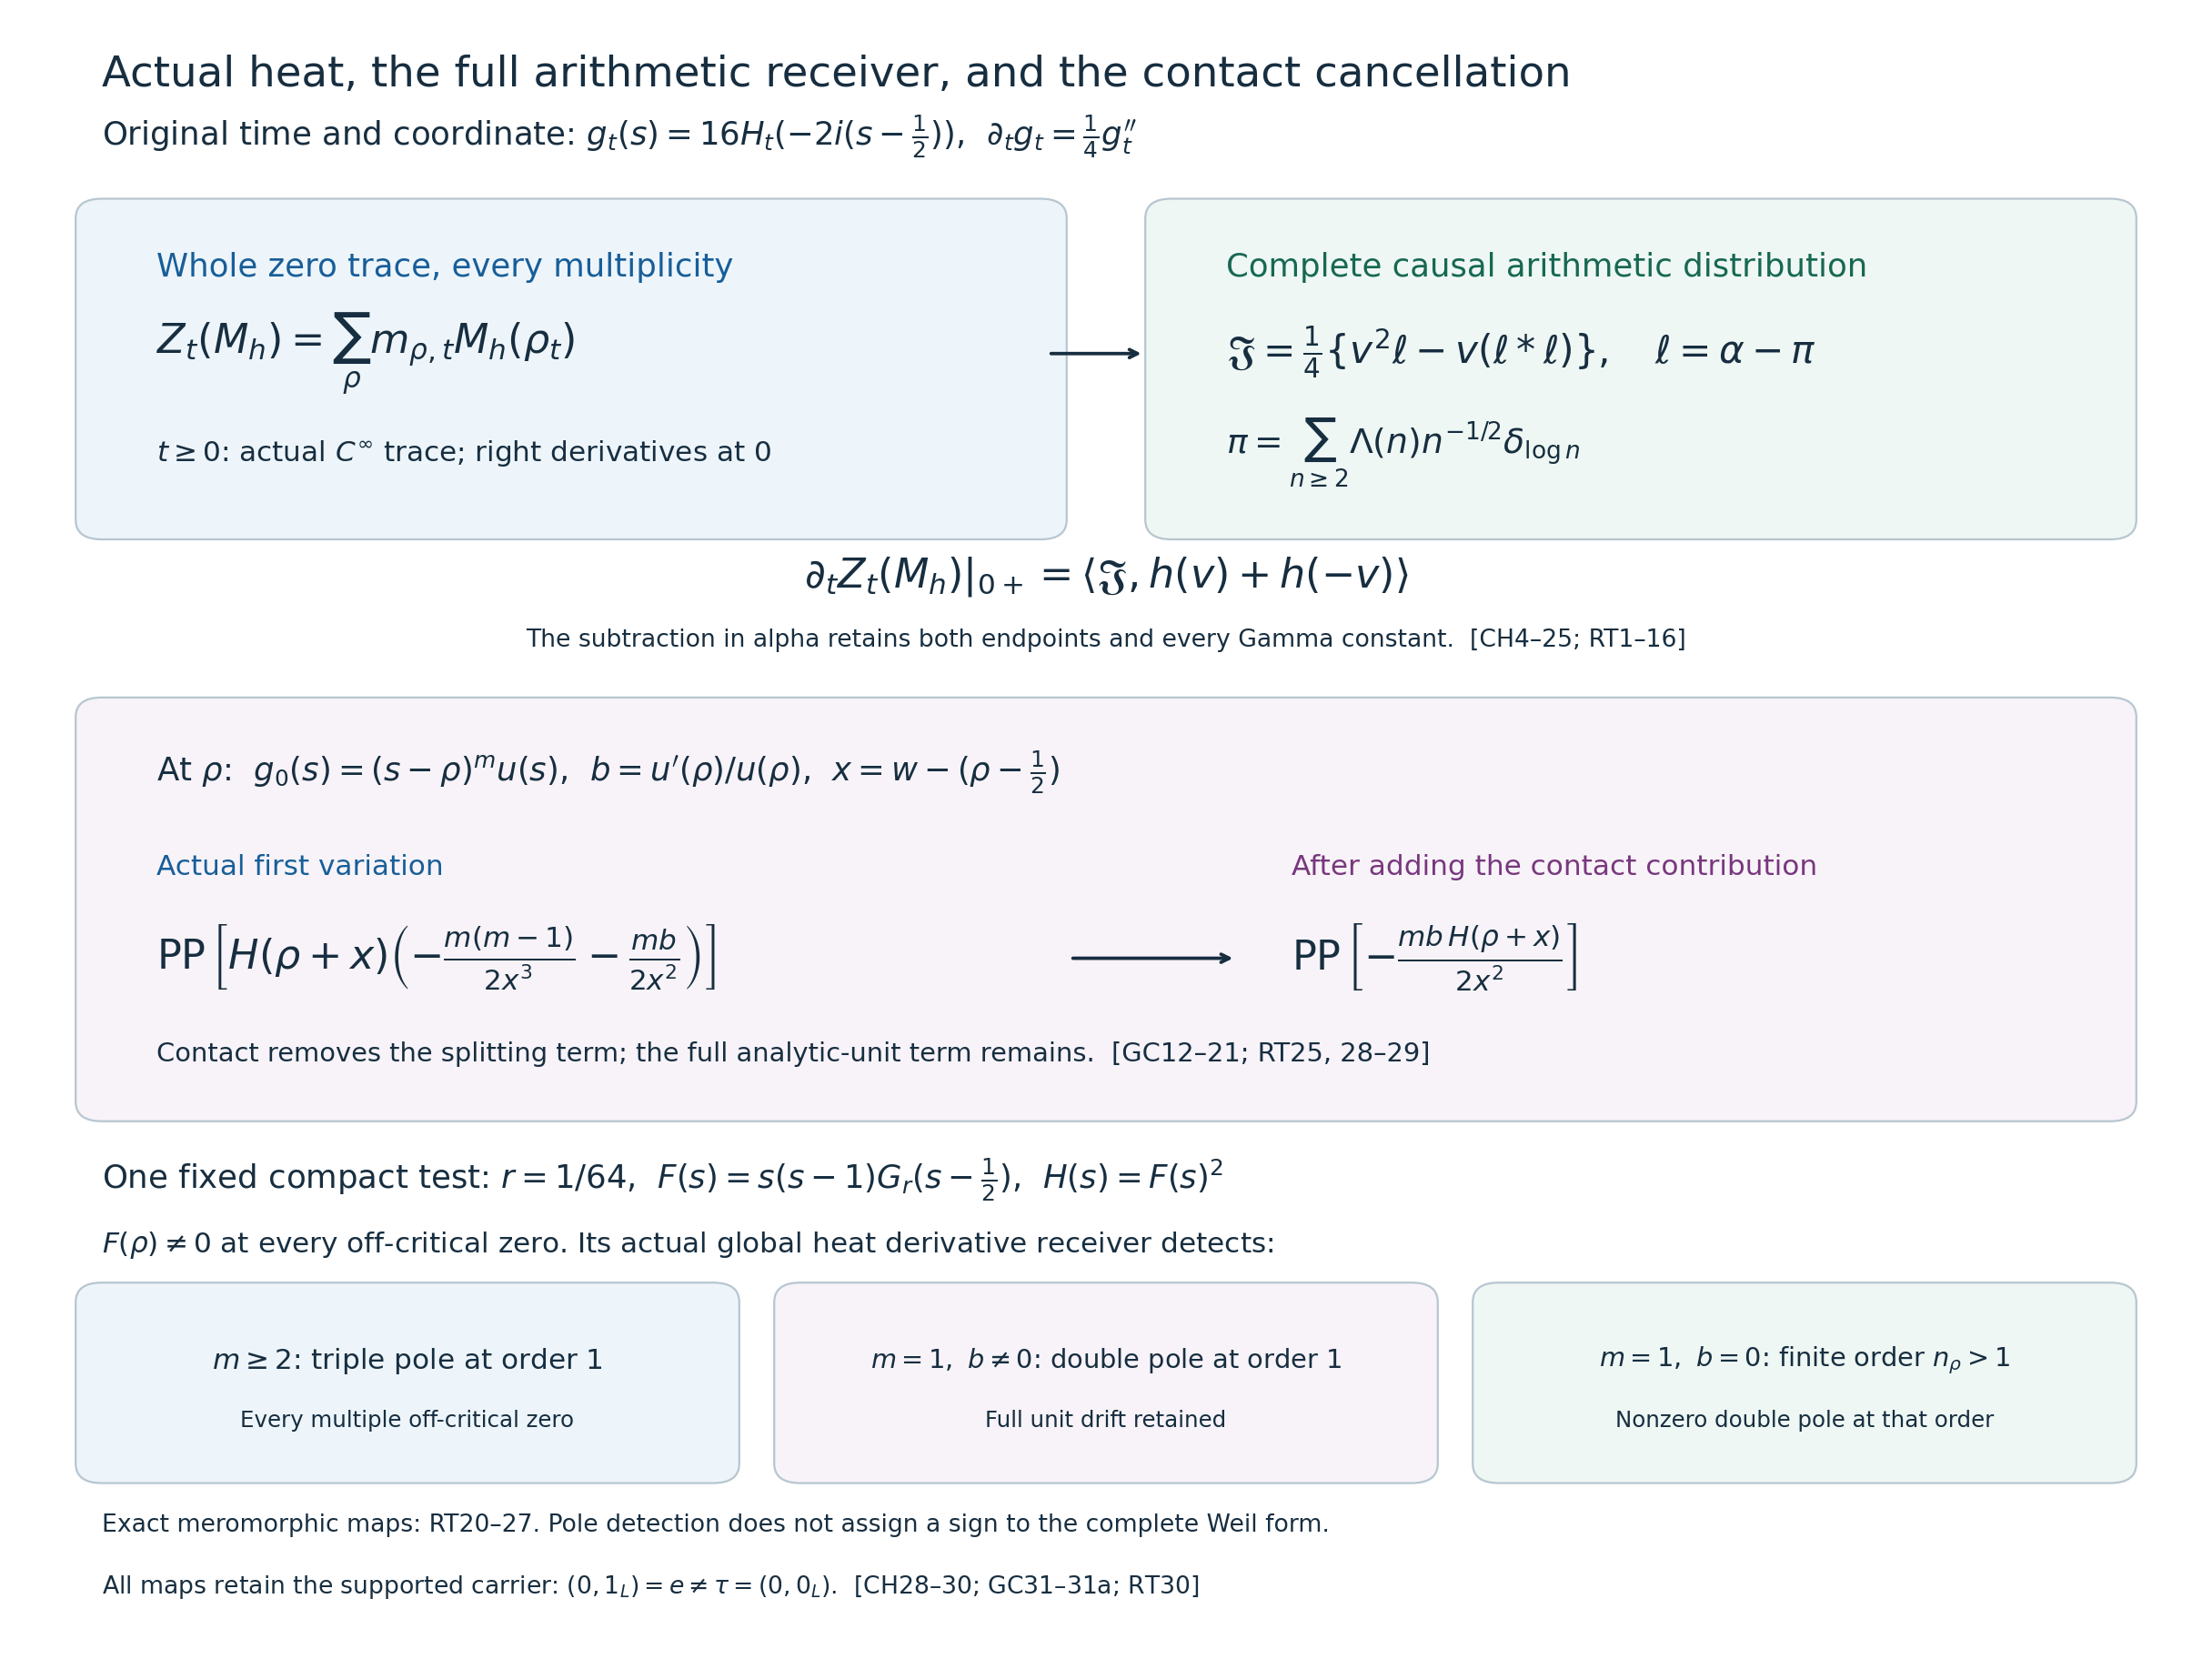
\includegraphics[keepaspectratio,alt={The actual positive-real-time trace and the full causal arithmetic distribution are related by RT16. At each zero, the middle panel displays the complete singular coefficient before and after the contact addition; PP means its principal part. The bottom panels distinguish multiple zeros, simple zeros with nonzero first velocity, and simple zeros whose first motion occurs at a higher order. The test H is the square F squared in RT17, with its original radius one over sixty-four. All constants, coordinates, signs and support labels are retained. Proofs: CH4--25, GC12--21, and RT1--30. Human input: the original Rodgers--Tao heat integral and de Bruijn's strip theorem as stated in Dobner's original author TeX. This exact diagram is not a sampled zero configuration or a positivity certificate.}]{actual_heat_contact.png}}
\caption{The actual positive-real-time trace and the full causal
arithmetic distribution are related by RT16. At each zero, the middle
panel displays the complete singular coefficient before and after the
contact addition; PP means its principal part. The bottom panels
distinguish multiple zeros, simple zeros with nonzero first velocity,
and simple zeros whose first motion occurs at a higher order. The test H
is the square F squared in RT17, with its original radius one over
sixty-four. All constants, coordinates, signs and support labels are
retained. Proofs: CH4--25, GC12--21, and RT1--30. Human input: the
original Rodgers--Tao heat integral and de Bruijn's strip theorem as
stated in Dobner's original author TeX. This exact diagram is not a
sampled zero configuration or a positivity certificate.}
\end{figure}

\subsection{Source identity and reading
coverage}\label{source-identity-and-reading-coverage}

The author archive for Dobner v2 is retained intact with SHA256
\texttt{21574649\allowbreak{}cdaae016\allowbreak{}f7da9087\allowbreak{}4f886f43\allowbreak{}91304ec7\allowbreak{}bd22808c\allowbreak{}2dad2c39\allowbreak{}7ec9be75}.
Its \texttt{paper.\allowbreak{}tex} has SHA256
\texttt{0de2b2f7\allowbreak{}e0d1178c\allowbreak{}a42a991c\allowbreak{}b803dae2\allowbreak{}ac0e24b7\allowbreak{}e6c9dae6\allowbreak{}a379e2f1\allowbreak{}6f4d9f31};
it is byte-identical to the indexed expanded author source. Actual
reading for this calculation covers lines 1--200 and 231--325, including
the full statement and application of \texttt{debruijnthm}. No complete
reading of that paper or its 1950 reference is claimed. The theorem
supplies (RT2); the uniform bounds, actual trace differentiability,
meromorphic derivative receiver, and exact maps (RT3)--(RT30) are proved
here. AG, HM, GC, CH, UP and PW are included in full in this edition,
with their original human sources and proof locators preserved.

\subsection{Proved compact-interval and finite-translation
bounds}\label{proved-compact-interval-and-finite-translation-bounds-4}

The complete \href{FIRST_PRIME_FULL_WEIL_COERCIVITY.md}{compact-interval
proof}, FC1--43, proves full Weil coercivity with constant 11509/600000
through support diameter 19/25, including prime 2 and both original
endpoint moments. \href{FIRST_PRIME_WINDOW_BOUND.md}{FW1--21} proves the
every-rank matrix bound for centre diameter 583/800 and a strict
two-test margin through the next prime gap. The same unchanged test now
satisfies its required strict correlation bound for every positive
translation through log 256, by
\href{FINITE_PRIME_WINDOW_EXTENSION.md}{FP1--25} and the complete
\href{FINITE_PRIME_WINDOW_COEFFICIENT_CERTIFICATE.md}{rational
prime-power certificate, FPC1--14}.
\href{PRIME_TWO_HEAT_TAIL_DERIVATION.md}{PT1--40} calculates the
surviving mixed channel and proves a strictly negative full actual right
heat derivative on the stated short interval after the prime-2 atom
ends. These are exact portions of the original bound, retaining
supported zero and every original arithmetic coefficient. The uniform
inequality beyond log 256 remains unproved.

\clearpage

\section{Full Weil coercivity across the first prime
window}\label{full-weil-coercivity-across-the-first-prime-window}

\textbf{Original-zeta receiving calculation.} The working meromorphic
function is the original Riemann zeta, with its full Gamma/endpoints
multiplier and its full trivial-zero and pole divisor retained.
\href{FAITHFUL_THETA_COMPLETION_RETURN.md}{TF1--42} proves the original
labelled theta inverse and the actual heat-image defect.
\href{FAITHFUL_UNCOMPLETED_ZETA_HEAT.md}{UZ1--53} proves every
exceptional-point fibre, jet, original-zeta heat term and reflection
orientation.
\href{ORIGINAL_ZETA_COMPACT_WEIL_RECONSTRUCTION.md}{OZC1--48} rederives
the compact contour and interval operator directly from zeta, including
the left-cutoff Gamma boundary, and specifies exactly which compensated
pairing the bounds concern.
\href{ORIGINAL_ZETA_HEAT_CONTACT_RECONSTRUCTION.md}{OZH1--49} rederives
the actual meromorphic heat, rational signed trace, compact-test domain,
contact drift and full causal arithmetic variation. The raw full divisor
and the compensated Weil receiver are linked by their displayed
correction, not identified. In particular the fixed-test trivial-zero
sum converges exactly at translations at least 1/32 and equals the
earlier R term; at zero translation it requires the proved cutoff
compensation. \href{ORIGINAL_ZETA_CAUCHY_RECONSTRUCTION.md}{OZK1--38}
reconstructs the original signed Cauchy trace, its full Gamma
correction, resonant finite parts, every finite matrix and its index,
and the complete local heat jets. Its invertible map retains the raw
trace and correction separately. These complete receiving proofs govern
the interpretation of the retained auxiliary calculations below.

The full reflected Weil form has an explicit positive lower bound on
every compact smooth test satisfying its two global endpoint equations
and supported in an interval of length at most \(19/25\). The
prime-\(2\) interaction is included. Its two overlap regions are
controlled by the exact archimedean boundary potential; the global
moment equations then control the two lowest Legendre modes.

Precisely, put \[
T_*=\frac{19}{25},\qquad c_*=\frac{11509}{600000}.
\tag{FC1}
\] For every nonzero complex-valued test in \[
\mathcal V_{T_*}=
\left\{F\in C_c^\infty(\mathbb R;\mathbb C):
\int F(t)e^{t/2}\,dt=\int F(t)e^{-t/2}\,dt=0,\
\operatorname{diam}(\operatorname{supp}F)\le T_*\right\},
\] the result is \[
\boxed{Q(F)>c_*\|F\|_2^2>\frac1{64}\|F\|_2^2.}
\tag{FC2}
\] For the zero function all terms are zero; the corresponding
non-strict inequality holds on the whole space.

This extends the supplied companion manuscript's \(3/4\)-support
calculation N48--N52. That incoming result and proof strategy are
retained as the source of the starting estimate; the larger support
width, its explicit constant, and the application of that width to the
entire first-prime window are the continuation here. Every estimate
needed for (FC2) is proved below. No numerical location of a zeta zero
is used, and no assertion of global Weil positivity or RH follows from
this local theorem.

\subsection{1. Original form, involution, and all endpoint
coordinates}\label{original-form-involution-and-all-endpoint-coordinates}

Use exactly \[
M_F(s)=\int_{\mathbb R}F(t)e^{-(s-1/2)t}\,dt,\qquad
F^\#(t)=\overline{F(-t)},\qquad
\tau_uF(t)=F(t-u),\qquad
\langle F,G\rangle=\int\overline F G.
\tag{FC3}
\] For \(h=F^\#*F\), \[
h(u)=\int\overline{F(t-u)}F(t)\,dt,\qquad
M_h(s)=\overline{M_F(1-\overline s)}M_F(s).
\] The full explicit formula, with every nontrivial zero and
multiplicity, is \[
\begin{aligned}
Q(F)&=\sum_\rho m_\rho
\overline{M_F(1-\overline\rho)}M_F(\rho)\\
&=M_h(0)+M_h(1)+A_\infty(h)-P_{\rm fin}(h),\\
P_{\rm fin}(h)&=
2\sum_{n\ge2}\frac{\Lambda(n)}{\sqrt n}
\Re\langle F,\tau_{\log n}F\rangle.
\end{aligned}
\tag{FC4}
\] Here \(\Lambda\) is the von Mangoldt function, with
\(\Lambda(p^j)=\log p\) and zero otherwise. Compact support makes the
prime sum finite. The original critical-strip zero count and rapid
vertical decrease of the compact smooth transforms prove absolute
convergence of the zero sum. The complete derivation, including the full
supported endpoints, is
\href{https://github.com/KokunoYumeto/zeta-function-research-reader/blob/5a89872598df0902b7c1393cf8e4692ca3010a95/workbenches/splitzero-tandem/branches/tau-zero-prime-positivity/SUPPORTED_ZERO_PRIME_WEIL_DERIVATION.md}{SZW19--SZW38}.

The two original endpoint equations imply \[
M_h(0)=\overline{M_F(1)}M_F(0)=0,\qquad
M_h(1)=\overline{M_F(0)}M_F(1)=0.
\tag{FC5}
\] They are global equations on \(F\). No separate moment equations will
be imposed on pieces of its support.

For comparison with the incoming plus-exponent convention, the exact map
is reflection: \[
(RF)(t)=F(-t),\qquad R^2=1,\qquad
M_F^+(s)=M_F(1-s)=M_{RF}(s).
\tag{FC6}
\] It is unitary on \(L^2\), preserves support diameter, and exchanges
the moments. It preserves \(Q\), as follows by relabelling the
absolutely convergent zero sum by \(\rho\mapsto1-\rho\). Thus the
original convention and the supplied convention are related by a proved
map, with no change to the Weil involution.

\subsection{2. The complete archimedean
expression}\label{the-complete-archimedean-expression}

With \(N=\|F\|_2^2\), the original Gamma contribution is \[
A_\infty(h)=-(\gamma_E+\log\pi)N+
\int_0^\infty
\frac{e^{-x}N-\tfrac12e^{-x/4}\{h(x/2)+h(-x/2)\}}
{1-e^{-x}}\,dx.
\tag{FC7}
\] This is HA13, also PS3, derived from the exact multiplier
\(\Re\psi(1/4+iy/2)-\log\pi\) in SZW24. The subtracted numerator makes
the integral converge at zero.

Put \[
k(u)=\frac{e^{-u/2}}{1-e^{-2u}}=\frac{e^{u/2}}{2\sinh u},
\qquad
\kappa_\infty=\log(8\pi)+\gamma_E+\frac\pi2.
\] Changing \(x=2u\) in (FC7) and using \(\|F-\tau_uF\|^2=2N-2\Re h(u)\)
gives \[
A_\infty(h)=
\int_0^\infty k(u)\|F-\tau_uF\|_2^2\,du-\kappa_\infty N.
\tag{FC8}
\] Here is an explicit scalar verification. First (FC7) is the negative
of \[
\{\log(4\pi)+\gamma_E\}N+
2\int_0^\infty\{\Re h(u)-e^{-u/2}N\}k(u)\,du.
\] The sum of those two expressions is \[
\log4\,N+
2N\int_0^\infty
\frac{e^{-2u}-e^{-u}}{1-e^{-2u}}\,du=0.
\] Next, with \(q=e^{-u/2}\), \[
2\int_0^\infty(1-e^{-u/2})k(u)\,du
=4\int_0^1\frac{dq}{(1+q)(1+q^2)}
=\log2+\frac\pi2.
\tag{FC9}
\] The partial fractions are \(\{2(1+q)\}^{-1}+(1-q)/\{2(1+q^2)\}\).
These identities prove (FC8), including the entire constant.

Equations (FC4)--(FC9) give the original full form on the two-moment
space: \[
Q(F)=\int_0^\infty k(u)\|F-\tau_uF\|_2^2\,du
-\kappa_\infty\|F\|_2^2
-2\sum_{n\ge2}\frac{\Lambda(n)}{\sqrt n}
\Re\langle F,\tau_{\log n}F\rangle.
\tag{FC10}
\] Near zero, \(\|F-\tau_uF\|_2\le u\|F'\|_2\); at infinity \(k\) decays
exponentially. This verifies the convergence used above. In particular,
the endpoint/Gamma term has not been replaced by a constant-only
approximation.

\subsection{3. Exact interval transport and exterior
potential}\label{exact-interval-transport-and-exterior-potential}

For a containing interval \(I=[c-T/2,c+T/2]\), use the unitary map \[
f(x)=(U_{T,c}F)(x)=\sqrt{\frac T2}\,F(c+Tx/2),
\qquad -1\le x\le1,
\] \[
F(t)=\sqrt{\frac2T}\,f(2(t-c)/T),\qquad
\|f\|_2=\|F\|_2.
\tag{FC11}
\] Translation preserves the full form:
\(M_{\tau_cF}(s)=e^{-c(s-1/2)}M_F(s)\), and the two factors in the
reflected pairing cancel. The transformed moments are exactly \[
\int_{-1}^1f(x)e^{ax}\,dx=
\int_{-1}^1f(x)e^{-ax}\,dx=0,\qquad a=T/4.
\tag{FC12}
\] The original scalar factors from the centre and Jacobian are nonzero.
The displayed equations are therefore equivalent to the original two
moments.

Let \[
\begin{aligned}
(\mathcal Lf)(x)&=\frac12\int_{-1}^1
\frac{f(x)-f(y)}{|x-y|}\,dy,\\
v(x)&=-\frac12\log(1-x^2),\qquad
r(s)=k(s)-\frac1{2s},\\
(\mathcal R_Tf)(x)&=\frac T2\int_{-1}^1
r(T|x-y|/2)f(y)\,dy.
\end{aligned}
\tag{FC13}
\] The exact archimedean operator transported by (FC11) is \[
\boxed{
A_{\infty,T}=\mathcal L+v-\log(\pi T)-\gamma_E-\mathcal R_T.
}
\tag{FC14}
\] To prove it, write the translation energy as
\(\frac12\int_{\mathbb R^2}k(|t-u|)|F(t)-F(u)|^2\,dt\,du\). Interior
pairs give the difference kernel after transport. Exterior pairs give
the diagonal potential \[
J(T(1+x)/2)+J(T(1-x)/2),\qquad
J(s)=\int_s^\infty k(u)\,du.
\] Direct differentiation and the limit at zero prove \[
J(s)=\operatorname{arctanh}(e^{-s/2})
+\arctan(e^{-s/2})
=-\frac12\log s+\log2+\frac\pi4-\int_0^s r(u)\,du.
\tag{FC15}
\] The interior diagonal part of \(r\) cancels the two integrals in
(FC15). Its off-diagonal part is \(-\mathcal R_T\). The remaining
exterior constant is \(-\log(T/2)+2\log2+\pi/2\). Subtracting
\(\kappa_\infty\) leaves \(-\log(\pi T)-\gamma_E\); the remaining
variable term is \(v(x)\). This proves (FC14), retaining the complete
exterior contribution.

\subsection{\texorpdfstring{4. Control the actual prime-\(2\) term for a
range of
widths}{4. Control the actual prime-2 term for a range of widths}}\label{control-the-actual-prime-2-term-for-a-range-of-widths}

For this section let \[
\frac34\le T\le\frac{19}{25},\qquad
\beta=\frac{\log2}{\sqrt2},\qquad
\delta=\frac{2\log2}{T}.
\tag{FC16}
\] One has \(\log2<T<\log3\) and \(1<\delta<2\). Thus only the prime
power \(2\) occurs in (FC10). Its full transported value is \[
\langle f,B_2f\rangle=
2\beta\Re\int_{-1+\delta}^1\overline{f(x)}f(x-\delta)\,dx
\le\beta\int_{|x|\ge\delta-1}|f(x)|^2\,dx.
\tag{FC17}
\] The inequality is \(2\Re(\overline zw)\le|z|^2+|w|^2\). The overlap
strips \([-1,1-\delta]\) and \([-1+\delta,1]\) are disjoint; changing
variables in the second squared term gives exactly the displayed
integral. No phase or part of the prime interaction is omitted.

The convergent positive series \[
\log2=2\sum_{j=0}^\infty\frac1{(2j+1)3^{2j+1}}
\tag{FC18}
\] follows by integrating the geometric series for \(1/(1-x^2)\) from
zero to \(1/3\). Its first two terms give \(\log2>56/81\). Therefore
uniformly over (FC16), \[
\delta-1>\frac{1261}{1539},\qquad
\left(\frac{1261}{1539}\right)^2-\frac7{11}
=\frac{911684}{26053731}>0.
\] The bound \(e<11/4\) gives \(1-e^{-1}<7/11\), so \(v(x)>1/2\)
throughout both overlap strips. Outside them \(v(x)\ge0\).

Also \(e^{7/10}>12013/6000>2\), by its first four positive terms; hence
\(\log2<7/10\). Since \(\sqrt2>7/5\), one has \(\beta<1/2\).
Consequently the complete prime term satisfies \[
\boxed{\int_{-1}^1v(x)|f(x)|^2\,dx-\langle f,B_2f\rangle\ge0.}
\tag{FC19}
\] The elementary estimate \(e<11/4\) used here follows, for example,
from \[
e<\sum_{j=0}^3\frac1{j!}+
\frac{1/4!}{1-1/5}
=\frac{87}{32}<\frac{11}{4}.
\] It also gives \(\log3>1\), verifying the claimed range of prime
terms.

\subsection{5. The global moments give a quantitative Legendre
gap}\label{the-global-moments-give-a-quantitative-legendre-gap}

The nonnegative Hermitian form of \(\mathcal L\) is \[
\mathcal E(f,g)=\frac14\int_{-1}^1\int_{-1}^1
\frac{\overline{f(x)-f(y)}(g(x)-g(y))}{|x-y|}\,dx\,dy.
\] For a monomial, factor \(x^n-y^n\), divide by \(x-y\), and integrate
each term with \(\operatorname{sgn}(x-y)\). This gives \[
\mathcal Lx^n=H_nx^n-
\sum_{j=1}^{\lfloor n/2\rfloor}\frac{x^{n-2j}}{2j},
\qquad H_n=\sum_{j=1}^n\frac1j,\quad H_0=0.
\tag{FC20}
\] Symmetry and degree preservation therefore give
\(\mathcal LP_n=H_nP_n\) for the Legendre polynomials. Put \[
p_n=\sqrt{\frac{2n+1}{2}}P_n,\qquad
c_n=\langle p_n,f\rangle.
\] For a finite Legendre projection \(p^{(N)}=\sum_{n=0}^Nc_np_n\), the
integral form gives \[
\mathcal E(f,f)=
\sum_{n=0}^NH_n|c_n|^2+
\mathcal E(f-p^{(N)},f-p^{(N)}).
\] Indeed \(\mathcal E(p_n,f)=H_n\langle p_n,f\rangle\), by Fubini, and
all these integrals are finite for smooth \(f\) and polynomials.
Nonnegativity and completeness of the Legendre basis imply \[
\mathcal E(f,f)\ge
\frac32\|f\|_2^2-\frac32|c_0|^2-\frac12|c_1|^2.
\tag{FC21}
\] No convergence assumption on an infinite operator expansion is
required.

The two equations (FC12) give orthogonality of \(f_{\rm even}\) to
\(\cosh(ax)\), and of \(f_{\rm odd}\) to \(\sinh(ax)\). With
\(p_0=1/\sqrt2\) and \(p_1=\sqrt{3/2}\,x\), Taylor's integral remainder
and Cauchy--Schwarz give \[
|c_0|^2\le A(T)\|f_{\rm even}\|_2^2,\qquad
|c_1|^2\le\frac5{21}A(T)\|f_{\rm odd}\|_2^2,\qquad
A(T)=\frac{(T/4)^4\cosh^2(T/4)}{20}.
\tag{FC22}
\] The two remainder inequalities are \[
|\cosh(ax)-1|\le\frac{a^2x^2\cosh a}{2},\qquad
|\sinh(ax)/a-x|\le\frac{a^2|x|^3\cosh a}{6}.
\] After squaring, \(\int_{-1}^1x^4dx=2/5\) and \(\int_{-1}^1x^6dx=2/7\)
give the constants \(1/20\) and \(1/84\), respectively.

The constant \(1/4\) in \(r\) gives exactly \[
\langle f,\mathcal R_T^{(0)}f\rangle
=\frac T8\left|\int_{-1}^1f(x)\,dx\right|^2
=\frac T4|c_0|^2.
\tag{FC23}
\] Combining (FC21)--(FC23), and using orthogonality of the even and odd
parts, proves \[
\mathcal E(f,f)-\langle f,\mathcal R_T^{(0)}f\rangle
\ge
\left\{\frac32-\left(\frac32+\frac T4\right)A(T)\right\}\|f\|_2^2.
\tag{FC24}
\] The odd deficit is \(5A(T)/42\), which is bounded by the displayed
even deficit. This retains the constant kernel and uses only the
original two global moments.

\subsection{6. A certified kernel bound with the original
scale}\label{a-certified-kernel-bound-with-the-original-scale}

The analytic function \(r\) at zero has expansion \[
r(z)=\sum_{j=0}^\infty b_jz^j,\qquad
b_j=\frac{2^jB_{j+1}(3/4)}{(j+1)!},
\] \[
(b_0,\ldots,b_8)=
\left(\frac14,-\frac1{48},-\frac1{32},
\frac7{11520},\frac5{1536},-\frac{31}{1935360},
-\frac{61}{184320},\frac{127}{309657600},
\frac{277}{8257536}\right).
\tag{FC25}
\] This follows from \[
\frac{e^{z/2}}{2\sinh z}
=\frac1{2z}\frac{2ze^{3z/2}}{e^{2z}-1}.
\] The nearest nonremovable singularities are \(z=\pm i\pi\), so \(r\)
is analytic on the closed disc of radius \(2\).

For \(z=x+iy\), \(|z|=2\), \[
|\sinh z|^2=\sinh^2x+\sin^2y
\ge x^2+\frac{\sin^22}{4}y^2\ge\sin^22.
\] The first inequality uses the decrease of \(\sin y/y\) on \([0,2]\);
its derivative has the sign of \(y\cos y-\sin y\), whose derivative is
\(-y\sin y<0\). The alternating sine series gives \[
\sin2>2-\frac{2^3}{3!}+\frac{2^5}{5!}-\frac{2^7}{7!}
=\frac{286}{315}>\frac9{10}.
\] Thus, on that circle, \[
|r(z)|\le\frac e{2\sin2}+\frac14
<\frac{16}{9}<2.
\tag{FC26}
\] Cauchy's estimate consequently bounds the degree-eight tail. Define
the explicit rational function \[
E(T)=\sum_{j=1}^8|b_j|T^j+
\frac{2(T/2)^9}{1-T/2}\qquad(0<T<2).
\tag{FC27}
\] Then \(|r(s)-1/4|\le E(T)\) for \(0\le s\le T\). For the nonconstant
remainder operator from (FC13), Schur's row and column bounds give \[
\|\widetilde{\mathcal R}_T\|\le T E(T).
\tag{FC28}
\] Every coefficient and the remainder scale are those of the actual
kernel.

Before substituting a width, (FC14), (FC19), (FC24), and (FC28) prove on
the whole interval (FC16) \[
\boxed{
Q(F)\ge c(T)\|F\|_2^2,\qquad
c(T)=\frac32-\log(\pi T)-\gamma_E
-T E(T)-\left(\frac32+\frac T4\right)A(T).
}
\tag{FC29}
\] This is an explicit bound for every width in a stated numerical
interval whose prime condition has already been proved. It does not
assume the missing sign of a residual operator. If desired, a rational
majorant for the moment quantity is \[
A(T)\le
\frac{(T/4)^4}{20(1-T^2/32)^2},
\] because \((2n)!\ge2^n\) gives \(\cosh(T/4)\le(1-T^2/32)^{-1}\) on
this range.

\subsection{\texorpdfstring{7. Evaluation at
\(T=19/25\)}{7. Evaluation at T=19/25}}\label{evaluation-at-t1925}

Here \(a=19/100\), and \[
\cosh a\le\frac{20000}{19639}<\frac{33}{32}.
\] Exact rational substitution in (FC22) gives \[
A(T_*)<
\frac{141919569}{2048000000000},
\] \[
\left(\frac32+\frac{T_*}{4}\right)
\frac{141919569}{2048000000000}
=\frac{23984407161}{204800000000000}
=\frac1{8000}
-\frac{1615592839}{204800000000000}
<\frac1{8000}.
\tag{FC30}
\] The kernel bound is exactly \[
E(T_*)=
\frac{4199809019840292631}{117180000000000000000}
=\frac9{250}-
\frac{18670980159707369}{117180000000000000000}
<\frac9{250}.
\] Consequently \[
T_* E(T_*)<\frac{171}{6250}.
\tag{FC31}
\]

For the scalar term, the elementary identity \[
\frac{22}{7}-\pi=
\int_0^1\frac{x^4(1-x)^4}{1+x^2}\,dx>0
\] gives \(\pi<22/7\). The exact positive exponential truncation \[
\sum_{j=0}^7\frac{(43/50)^j}{j!}
-\frac{33}{14}
=\frac{1126807544917}{187500000000000}>0
\] proves \(\log(33/14)<43/50\). For Euler's constant, monotonicity of
\(H_n-\log n\), together with the first four terms of (FC18), gives \[
\gamma_E<H_{256}-8\log2
<\frac{612435}{100000}-8\frac{53056}{76545}
=\frac{177361483}{306180000}<\frac{29}{50}.
\tag{FC32}
\] Here \(H_{256}<612435/100000\) is a finite exact rational sum,
checked independently by the accompanying source. Therefore \[
\log(3\pi/4)+\gamma_E<\frac{43}{50}+\frac{29}{50}=\frac{36}{25}.
\] Since \(T_*/(3/4)=76/75\) and \(\log(1+x)<x\) for \(x>0\), \[
\boxed{
\log(\pi T_*)+\gamma_E
<\frac{36}{25}+\frac1{75}=\frac{109}{75}.
}
\tag{FC33}
\]

Substitute (FC30)--(FC33) into (FC29). For nonzero \(F\), \[
\begin{aligned}
Q(F)&>
\left(\frac32-\frac{109}{75}-\frac{171}{6250}-\frac1{8000}\right)
\|F\|_2^2\\
&=\frac{11509}{600000}\|F\|_2^2.
\end{aligned}
\tag{FC34}
\] Its margin above \(1/64\) is exactly \(1067/300000>0\), proving
(FC2).

There is also a separate, slightly weaker rational scalar route. The
five terms \[
\sum_{j=0}^4\frac{(7/8)^j}{j!}
=\frac{78443}{32768}
>\frac{418}{175}>\pi T_*
\] give \(\log(\pi T_*)+\gamma_E<291/200\), and hence \[
Q(F)>\frac{3503}{200000}\|F\|_2^2>
\frac1{64}\|F\|_2^2.
\tag{FC35}
\] The stronger constant in (FC34) exceeds this by exactly \(1/600\).
Both estimates use the same full operator and prime term.

\subsection{8. Exact support range of the fixed first-prime
tests}\label{exact-support-range-of-the-fixed-first-prime-tests}

For the programme's fixed radius \(r=1/64\), the test \(f_r\) has
support in \([-r,r]\). Its autocorrelation has support in \([-2r,2r]\),
so the possible first-prime translation window is \[
\log2-2r\le a\le\log2+2r.
\] The union of the supports of \(f_r\) and \(\tau_af_r\) has containing
interval length at most \(a+2r\). Throughout this window it is therefore
at most \[
\log2+4r=\log2+\frac1{16}.
\tag{FC36}
\] This is below \(19/25\), with a rational proof. The first five
positive terms of \(e^{25/36}\) exceed \(2\), so \(\log2<25/36\). Then
\[
\log2+\frac1{16}<\frac{109}{144}<\frac{19}{25},
\qquad \frac{19}{25}-\frac{109}{144}=\frac{11}{3600}>0.
\tag{FC37}
\] The finite exponential comparison is included in the exact checker.
Thus the larger coercive support interval covers the entire first-prime
window for these original-radius tests, including every linear
combination of the two translates. The complete fixed-test correlation
calculation uses this inclusion; no outside-window bound is inferred
here.

\subsection{9. Original primitives, finite matrices, and supported
zero}\label{original-primitives-finite-matrices-and-supported-zero}

The endpoint-killing operator is unchanged: \[
\mathcal D=\partial_t^2-\frac14,\qquad
M_{\mathcal Dg}(s)=s(s-1)M_g(s).
\tag{FC38}
\] The identity follows by two integrations by parts for
\(g\in C_c^\infty\), and \(\mathcal D\) does not enlarge support.
Conversely every compact smooth \(F\) satisfying the two moments has the
unique compact smooth primitive \[
g(t)=-\int_{\mathbb R}e^{-|t-u|/2}F(u)\,du,\qquad
\mathcal Dg=F.
\tag{FC39}
\] The kernel has derivative jump one. Outside a containing support
interval, its two tails are the original two exponential moments and
hence vanish. A difference of two compact primitives solves the
homogeneous equation and must be zero. Thus (FC39) preserves the
containing support interval.

The norm calculation gives \[
\|\mathcal Dg\|_2^2=
\|g''\|_2^2+\frac12\|g'\|_2^2+\frac1{16}\|g\|_2^2.
\] Consequently, for nonzero \(g\) with support diameter at most
\(19/25\), \[
Q(\mathcal Dg)>
c_*\left(\|g''\|_2^2+\frac12\|g'\|_2^2+\frac1{16}\|g\|_2^2\right).
\tag{FC40}
\] The interval coordinate map has the exact intertwining formula \[
U_{T,c}\mathcal D U_{T,c}^{-1}
=\frac4{T^2}\partial_x^2-\frac14.
\tag{FC41}
\] No constant has been absorbed into a different differential operator.

For a finite family in one common containing interval of length
\(19/25\), the full sesquilinear form satisfies \[
[Q(F_i,F_j)]\succeq c_*[\langle F_i,F_j\rangle].
\tag{FC42}
\] Apply (FC34) to \(\sum c_jF_j\) to prove the matrix statement; the
difference is strictly positive whenever that function is nonzero.

Finally retain the entire original support space \(\mathbb C[L]\). With
\(H=M_{F^\#*F}\), its distributions are \[
\begin{aligned}
\boldsymbol B_L&=(H(0)+H(1))\mathbf e_{1_L}
+H(0)\sum_{\lambda\ne1_L}\mathbf e_\lambda,\\
\boldsymbol Z_L&=Q(F)\mathbf e_{1_L},\\
\boldsymbol D_L&=(P_{\rm fin}-A_\infty)\mathbf e_{1_L}
+H(0)\sum_{\lambda\ne1_L}\mathbf e_\lambda,\\
\boldsymbol B_L-\boldsymbol Z_L&=\boldsymbol D_L.
\end{aligned}
\tag{FC43}
\] Both endpoint coefficients vanish by (FC5); their coordinate spaces
remain. Every linear map displayed above has the fixed-label lift
\((F,\lambda)\mapsto(TF,\lambda)\) on its stated domain. It commutes
with amplitude projection and leaves the support label unchanged. A zero
amplitude in such a carrier remains its supported zero \((0,\lambda)\);
it is not identified with the unsupported element \(\tau\).

\subsection{Source and verification
record}\label{source-and-verification-record}

The starting \(3/4\) theorem and interval-operator method were supplied
in the companion manuscript ``Direct RH continuation: the optimal packet
cost in the full Weil form,'' N1--N11 and N48--N52, dated 23 September
2026, source SHA256
D3B1AC08C71F6104CFE011BA5E5B86F6FBE182916C0B0270511671B1F7165D5B. The
independent audit is retained separately. The present proof gives all
arguments needed for the enlarged interval and its stronger constant.

The programme's original full formula is SZW19--SZW38, with its human
Weil and Connes sources; HA13 supplies the real kernel (FC7), and
PS1--PS15 supplies the original support and primitive conventions, which
are rederived where used here. No historical priority claim is made for
the interval kernel, Legendre diagonalization, or local Weil positivity.

The accompanying exact-rational checker divides the kernel power series
independently, verifies every displayed rational estimate at \(3/4\) and
\(19/25\), evaluates the finite harmonic sum, and checks the exponential
comparisons. It uses rational arithmetic only. These checks supplement
the analytic estimates (FC7)--(FC43); they do not replace the
convergence, domain, or prime-interaction proofs.

\clearpage

\section{A proved bound over the complete first prime
window}\label{a-proved-bound-over-the-complete-first-prime-window}

\textbf{Original-zeta receiving calculation.} The working meromorphic
function is the original Riemann zeta, with its full Gamma/endpoints
multiplier and its full trivial-zero and pole divisor retained.
\href{FAITHFUL_THETA_COMPLETION_RETURN.md}{TF1--42} proves the original
labelled theta inverse and the actual heat-image defect.
\href{FAITHFUL_UNCOMPLETED_ZETA_HEAT.md}{UZ1--53} proves every
exceptional-point fibre, jet, original-zeta heat term and reflection
orientation.
\href{ORIGINAL_ZETA_COMPACT_WEIL_RECONSTRUCTION.md}{OZC1--48} rederives
the compact contour and interval operator directly from zeta, including
the left-cutoff Gamma boundary, and specifies exactly which compensated
pairing the bounds concern.
\href{ORIGINAL_ZETA_HEAT_CONTACT_RECONSTRUCTION.md}{OZH1--49} rederives
the actual meromorphic heat, rational signed trace, compact-test domain,
contact drift and full causal arithmetic variation. The raw full divisor
and the compensated Weil receiver are linked by their displayed
correction, not identified. In particular the fixed-test trivial-zero
sum converges exactly at translations at least 1/32 and equals the
earlier R term; at zero translation it requires the proved cutoff
compensation. \href{ORIGINAL_ZETA_CAUCHY_RECONSTRUCTION.md}{OZK1--38}
reconstructs the original signed Cauchy trace, its full Gamma
correction, resonant finite parts, every finite matrix and its index,
and the complete local heat jets. Its invertible map retains the raw
trace and correction separately. These complete receiving proofs govern
the interpretation of the retained auxiliary calculations below.

This calculation applies the full compact-interval estimate to the
original fixed test of UP and PW. It proves the required
translated-correlation bound on a specified interval containing the
whole contribution of prime two, with a strict margin. It retains the
negative archimedean cross term and both signs of the two-test Weil
form. The calculation does not extend its proved interval to arbitrary
translations.

\subsection{1. Original test, form, and exact local
estimate}\label{original-test-form-and-exact-local-estimate}

Retain the original conventions \[
M_f(s)=\int_{\mathbb R}f(v)e^{-(s-1/2)v}\,dv,\qquad
f^\#(v)=\overline{f(-v)},\qquad
T=\partial_v^2-\tfrac14,
\tag{FW1}
\] and the complete original pairing \[
B(f,g)=\sum_\rho m_\rho\overline{M_f(1-\bar\rho)}M_g(\rho),
\qquad Q(f)=B(f,f).
\tag{FW2}
\] The zeros are the actual nontrivial zeta zeros with their actual
multiplicities. The absolute convergence and the complete supported
explicit formula are proved in PW1--2 and SZW24--38. No endpoint is
removed without evaluating its moment.

Use exactly the fixed density and test \[
\begin{gathered}
r=\tfrac1{64},\qquad
b_r=\mathop{*}_{j\ge1}\frac{\mathbf1_{[-r2^{-j},r2^{-j}]}}{2r2^{-j}},\qquad
f_r=Tb_r,\\
k_r=b_r*b_r,\qquad h_r=f_r*f_r=T^2k_r,\qquad
N_r=\|f_r\|_2^2>0.
\end{gathered}\tag{FW3}
\] Their full construction and Fourier product are retained in UP1--14
and PW3--5, including the classical compact bump attribution. The
functions are real, even and smooth, with supports of \(b_r,f_r\)
contained in \([-r,r]\) and those of \(k_r,h_r\) contained in
\([-2r,2r]\). Also \(k_r\ge0\), \(\int k_r=1\), and \(h_r(0)=N_r\).
Twice integrating by parts gives \(M_{f_r}(s)=s(s-1)G_r(s-1/2)\), so
both endpoint moments vanish exactly.

The complete proof \href{FIRST_PRIME_FULL_WEIL_COERCIVITY.md}{FC, full
first-prime interval coercivity} establishes, with all prime-two and
Gamma terms retained, \[
Q(F)>c_*\|F\|_2^2\quad(F\ne0),\qquad
c_*:=\frac{11509}{600000}>\frac1{64},\qquad
\operatorname{diam}(\operatorname{supp}F)\le T_*:=\frac{19}{25},
\tag{FW4}
\] for every compact smooth complex test satisfying \(M_F(0)=M_F(1)=0\).
For \(F=0\), the corresponding non-strict inequality is equality. The
source derives (FW4) from the full compact-interval operator, the exact
two moments, the boundary potential dominating the prime-two
translation, and a rational bound for its analytic remainder. This proof
uses that entire result, without imposing separate moment conditions on
pieces of a test.

Define the actual translated quantities \[
f_a(v)=f_r(v-a),\qquad
K(a)=B(f_a,f_r),\quad q=K(0),\quad
C(a)=\langle f_a,f_r\rangle_{L^2}=h_r(a),\quad
A_*:=T_*-2r=\frac{583}{800}.
\tag{FW5}
\] Here \(K\) is real and even by PW6--8, and \(B(f_a,f_b)=K(a-b)\),
while \(\langle f_a,f_b\rangle=C(a-b)\). These equalities follow by a
change of variable for Haar measure and cancellation of the two
translation exponentials in (FW2). The complete diagonal is \(q\),
unchanged by translation. In particular (FW4) on the single nonzero test
proves \(q>c_*N_r\).

\subsection{2. Every finite rank on the specified translation
interval}\label{every-finite-rank-on-the-specified-translation-interval}

Let \(a_1,\ldots,a_n\) be distinct real numbers with
\(\max a_j-\min a_j\le A_*\). For every coefficient vector
\(z\in\mathbb C^n\), set \[
F_z=\sum_{j=1}^n z_j f_{a_j}.
\tag{FW6}
\] Each summand has both endpoint moments zero: translation multiplies
those moments by \(e^{-(s-1/2)a_j}\), which leaves their zero values
unchanged. Hence \(F_z\) has the original two global moments zero. Its
support is contained in \([\min a_j-r,\max a_j+r]\), whose length is at
most \(T_*\).

For \(z\ne0\), this test is nonzero. To prove linear independence of
these actual translates, take the Fourier transform of a putative zero
relation. The transform of \(f_r\) is nonzero on an open real interval
because it is an entire function that is not identically zero. On that
interval the relation forces \(\sum z_j e^{-i a_j y}=0\). This entire
exponential polynomial is then identically zero. Its first \(n\)
derivatives at zero give the Vandermonde system with determinant
\(\prod_{i<j}(-ia_j+ia_i)\ne0\); all \(z_j\) vanish. This proves the
assertion for every finite distinct centre list.

Applying (FW4) to (FW6) and expanding both forms gives the exact matrix
inequality \[
\boxed{
[K(a_i-a_j)]_{i,j=1}^n
-c_*[h_r(a_i-a_j)]_{i,j=1}^n\succ0
\quad\text{when }\max a_j-\min a_j\le\frac{583}{800}.}
\tag{FW7}
\] It holds at every finite rank on this specified interval. Repeated
centres can instead be retained, giving the non-strict inequality and
the exact kernel of their coefficient-summing map. No finite-rank
conclusion is extrapolated to centre lists with larger diameter.

\subsection{3. The exact two-translate bound and its strict
margin}\label{the-exact-two-translate-bound-and-its-strict-margin}

For \(0<a\le A_*\), the two-by-two instance of (FW7) has diagonal
\(q-c_*N_r>0\) and real off-diagonal \(K(a)-c_*h_r(a)\). Its two
eigenvalues are the diagonal plus and minus that off-diagonal. Both are
positive. Therefore \[
\boxed{|K(a)-c_*h_r(a)|<q-c_*N_r\qquad(0<a\le583/800).}
\tag{FW8}
\] At \(a=0\) the corresponding inequality is equality. When
\(a\ge2r=1/32\), the two translated supports overlap at most at an
endpoint and \(h_r(a)=0\). Thus \[
\boxed{|K(a)|<q-c_*N_r<q
\qquad\left(\frac1{32}\le a\le\frac{583}{800}\right).}
\tag{FW9}
\] For \(0<a<2r\), Haar Cauchy--Schwarz gives \(|h_r(a)|\le N_r\), and
(FW8) also implies \(|K(a)|<q\). Consequently the original RH-equivalent
inequality is proved throughout \([0,583/800]\); its value at zero is
the stated equality. Its unproved part consists of larger translations.

In particular both original signed two-test values satisfy \[
Q(f_r+f_a)=2q+2K(a)>2c_*N_r,\qquad
Q(f_r-f_a)=2q-2K(a)>2c_*N_r
\tag{FW10}
\] on the interval in (FW9). Both tests retain their exact endpoint-zero
support carriers. The sign of their off-diagonal correlation has not
been substituted for the sign of either quadratic form.

\subsection{4. The whole prime-two contribution and the negative cross
term}\label{the-whole-prime-two-contribution-and-the-negative-cross-term}

Put \(L=\log2\) and \(\beta=L/\sqrt2\). The exact first prime window is
\[
I_2=[L-1/32,L+1/32].
\tag{FW11}
\] It lies strictly inside the interval in (FW9). Here is a rational
verification of the required endpoint comparison. The convergent
identity \(\log2=2\sum_{j\ge0}[(2j+1)3^{2j+1}]^{-1}\) follows by
integrating the geometric series for \((1-x^2)^{-1}\) from zero to
\(1/3\). Its first four terms give a lower bound greater than \(2/3\).
Bounding every denominator in the remaining tail below by nine gives \[
\log2\le
2\sum_{j=0}^{3}\frac1{(2j+1)3^{2j+1}}
+\frac1{4\cdot3^9}
<\frac{139}{200}.
\tag{FW12}
\] The last comparison is between rational numbers. Hence
\(L+1/16<139/200+1/16=303/400<19/25\), proving \(L+1/32<A_*\). The lower
window endpoint exceeds \(1/32\) because \(L>2/3>1/16\).

For every \(1/32<a\le A_*\), only the prime power two can occur in the
full PW13 sum: its largest possible index satisfies
\(\log n\le a+1/32\le19/25<1<\log3\), the last inequality following from
\(e<11/4<3\). All terms with indices at least three vanish through the
test support, with their labelled coordinates retained. The complete
correlation is therefore \[
\boxed{K(a)=-R_r(a)-\beta h_r(a-L),}
\qquad
R_r(a)=\int_{a-1/32}^{a+1/32}W(v)k_r(a-v)\,dv>0,
\tag{FW13}
\] where the unchanged explicit kernel is \[
W(v)=\frac{4e^{-5v/2}(9+55e^{-2v}+31e^{-4v}+e^{-6v})}
{(1-e^{-2v})^5},\qquad v>0.
\tag{FW14}
\] PW15--17 proves these identities by four integrations by parts with
the actual filter \(T^2\). Combining (FW9) and (FW13) proves the full
arithmetic estimate \[
\boxed{\left|R_r(a)+\frac{\log2}{\sqrt2}h_r(a-\log2)\right|
<q-\frac{11509}{600000}\|f_r\|_2^2
\quad\left(\frac1{32}<a\le\frac{583}{800}\right).}
\tag{FW15}
\] This covers the entire window \(I_2\), including the two endpoints
where the prime-two amplitude vanishes. The smaller-support terms have
not been compared separately by assigning them unproved signs.

At its centre the complete off-diagonal value and resulting diagonal
estimate are especially explicit: \[
K(\log2)=-R_r(\log2)-\frac{\log2}{\sqrt2}N_r<0,
\qquad
q>\left(\frac{\log2}{\sqrt2}+c_*\right)N_r+R_r(\log2).
\tag{FW16}
\] The inequality is exactly (FW15) with \(h_r(0)=N_r\). This strictly
negative cross term is compatible with the strict positivity of both
signed quadratic tests in (FW10); all four terms of their bilinear
expansion are retained.

\subsection{5. Original supported-zero maps and the remaining
translations}\label{original-supported-zero-maps-and-the-remaining-translations}

Let \(\mathscr L\) be the original nontrivial bounded distributive
support lattice. The linear map \(z\mapsto F_z\), each translation, the
moment map, and \(T\) have the exact fixed-carrier lift
\((x,\lambda)\mapsto(Ax,\lambda)\). Addition uses the original join, and
scalar multiplication uses the original meet. Direct substitution proves
additivity and scalar compatibility, as in UP34. The endpoint map sends
every top-labelled test in (FW6) to \((0,1_{\mathscr L})\), while the
unsupported input remains \((0,0_{\mathscr L})\). The zero endpoint
amplitude therefore retains supported zero \(e\ne\tau\).

The pairing lift is \[
B^{\mathscr L}((u,\lambda),(v,\mu))=(B(u,v),\lambda\wedge\mu).
\tag{FW17}
\] Its compatibility follows from sesquilinearity and distributivity. In
particular the finite Gram matrices in (FW7) are values of the existing
lifted form, not replacement support spaces. On the translated
convolution the original full formula has \[
\boldsymbol B_{\mathscr L}=0,\qquad
\boldsymbol Z_{\mathscr L}=K(a)\mathbf e_{1_{\mathscr L}},\qquad
\boldsymbol D_{\mathscr L}=-K(a)\mathbf e_{1_{\mathscr L}}.
\tag{FW18}
\] All lower coordinate functionals have their evaluated zero endpoint
amplitudes; their coordinate spaces and support labels persist. Formula
(FW13) is their top amplitude, with the actual prime-two coefficient and
entire archimedean term.

\subsection{6. Continue the two-test estimate across the following prime
gap}\label{continue-the-two-test-estimate-across-the-following-prime-gap}

The first estimate also supplies a bound on the next full gap, without
changing the fixed test. Put \[
A_3=\log3-2r=\log3-\frac1{32}.
\tag{FW19}
\] The exact inequalities already proved give \(\log2+2r<A_*<A_3\): the
left comparison is (FW12), and the right follows from \(\log3>1\) and
\(A_*<1-1/32\). For \(A_*\le a\le A_3\), prime two lies strictly below
the support window. Every \(n\ge3\) lies above it, except that \(n=3\)
meets its upper endpoint when \(a=A_3\). At that endpoint its value is
\(h_r(-2r)=0\), since \(h_r\) is smooth and supported in \([-2r,2r]\).
The complete finite-prime sum therefore vanishes on this closed
interval.

PW16 gives the absolutely convergent positive series, differentiable on
every compact subset of \(a>2r\), \[
R_r(a)=\sum_{j\ge1}4j^2(2j+1)^2
G_r(2j+1/2)^2e^{-(2j+1/2)a},\qquad R_r'(a)<0.
\tag{FW20}
\] Every coefficient is strictly positive because
\(G_r(x)=\int b_r(v)e^{-xv}\,dv>0\) on the real axis. Its growth bound
\(G_r(x)\le e^{r|x|}\) makes the differentiated series uniformly
convergent when \(a\) is bounded away from \(2r\). The full formula
consequently gives \(K(a)=-R_r(a)\) throughout this gap. At \(A_*\),
(FW9) gives \(R_r(A_*)<q-c_*N_r\). Monotonicity now proves \[
\boxed{|K(a)|<q-c_*N_r<q\qquad
\frac1{32}\le a\le\log3-\frac1{32}.}
\tag{FW21}
\] For the first part of this interval use (FW9); for its remaining part
use (FW20). Both inequalities (FW10) extend over the whole interval in
(FW21). Together with (FW8), this proves \(|K(a)|<q\) for every
\(0<a\le A_3\), and equality at \(a=0\). The every-rank matrix theorem
(FW7) retains its stated diameter \(583/800\); this prime-gap argument
extends the two-test bound and does not assert that larger matrix
theorem.

The full criterion PW20 still requires the inequality for
\(a>\log3-1/32\). The results here prove a strict margin on the complete
first-prime window, its following gap, and all finite centre
configurations of the stated smaller diameter. They do not establish the
remaining global inequality or infer RH from a finite interval.

\subsection{Sources and attribution}\label{sources-and-attribution}

The incoming programme note \emph{Direct RH continuation: the optimal
packet cost in the full Weil form}, dated 23 September 2026, supplied
the complete compact-interval operator and the rational
three-quarter-support estimate at N1--16 and N48--52. Its original
source SHA256 is
\texttt{d3b1ac08\allowbreak{}c71f6104\allowbreak{}cfe011ba\allowbreak{}5e5b86f6\allowbreak{}fbe18291\allowbreak{}6c0b0270\allowbreak{}511671b1\allowbreak{}f7165d5b};
it contains 84 equation tags in the N1--N60 and G1--G18 systems,
including suffixes. Root read that complete source. FC reproduces the
full mathematical ingredients used here, checks the incoming bound, and
proves its explicit extension to 19/25. The incoming author's
packet-cost claims are not needed for (FW1)--(FW18). The precise
application to the unchanged UP/PW test, every-rank local Gram, strict
correlation margin, whole first-prime window, and supported maps is
proved above. The complete original programme dependencies accompany
this edition, with their human citations and classical compact-bump
attribution retained.

\subsection{Exact objects and proved
bounds}\label{exact-objects-and-proved-bounds}

\begin{figure}
\centering
\pandocbounded{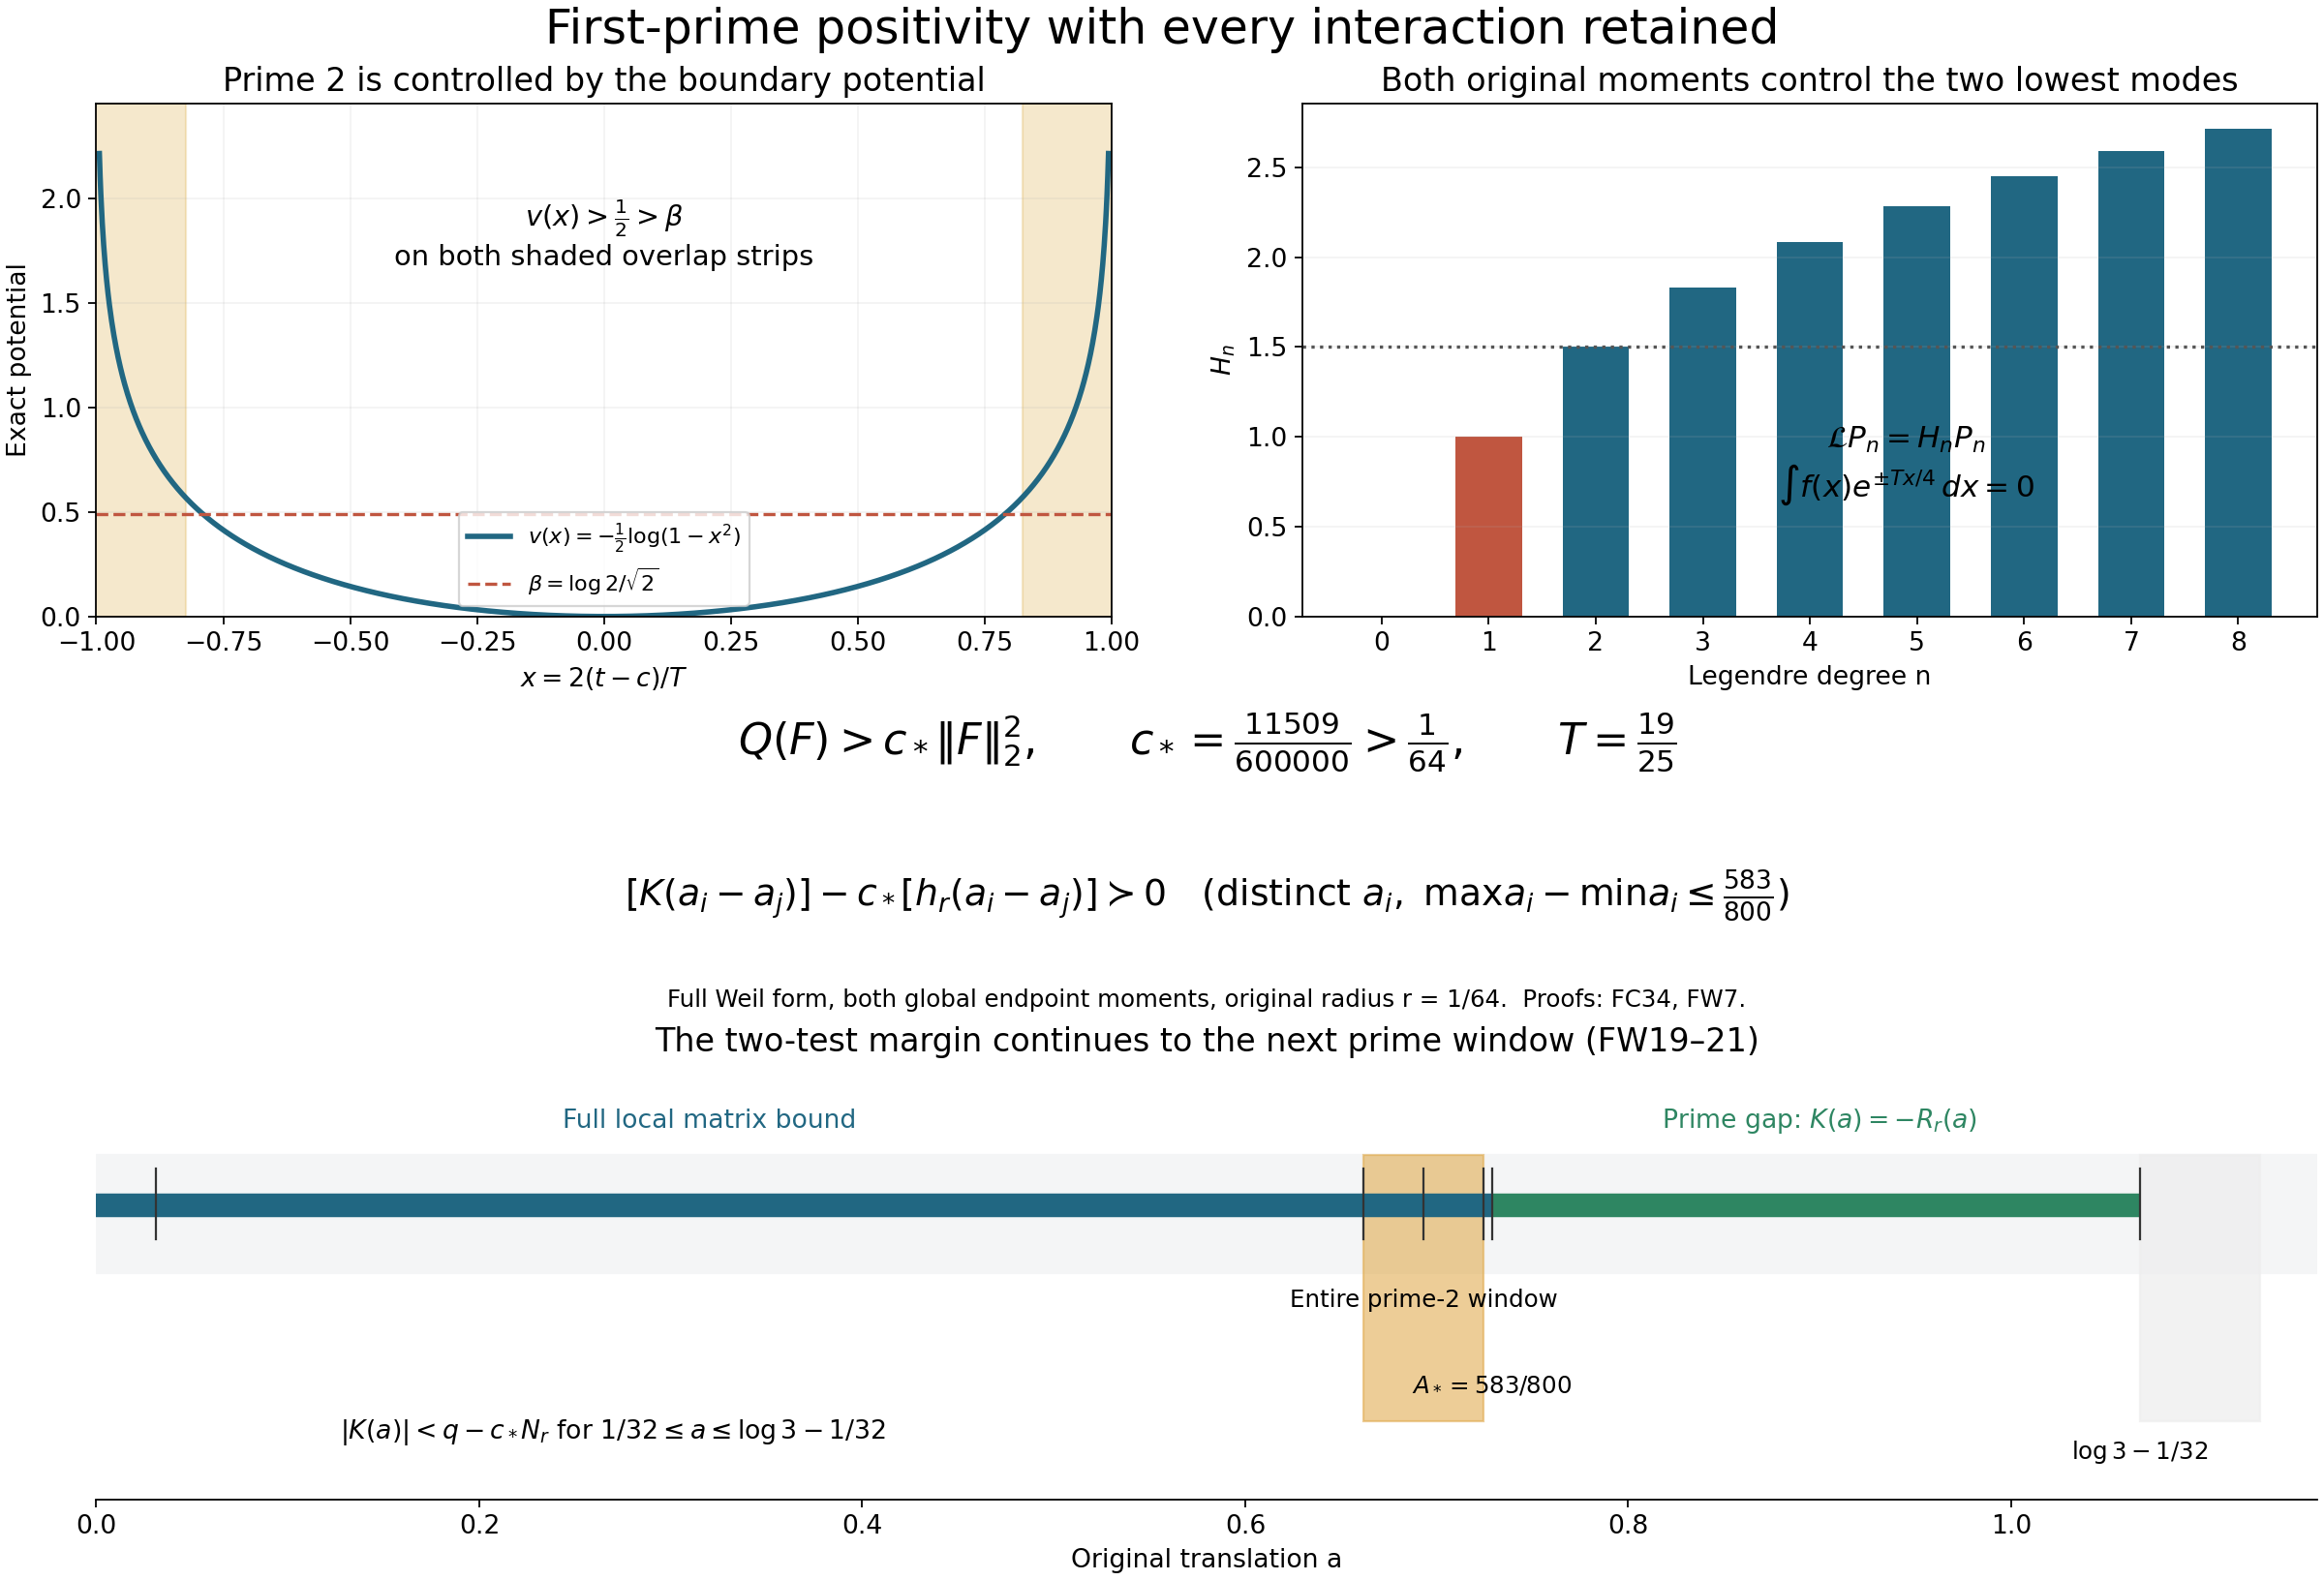
\includegraphics[keepaspectratio,alt={The full first-prime calculation. Shading shows the exact two overlap strips of the prime-2 shift in the original interval coordinate; the curve is the actual boundary potential. Harmonic-number bars show the Legendre eigenvalues, with the two global moments controlling degrees zero and one. The lower diagram gives the precise domains of the every-rank matrix bound and the longer two-test bound through the following gap. All constants, support widths and signs are those of FC19--34 and FW7--21. The classical compact density is identified with Arias de Reyna Theorem 1 by UP0. This diagram is not a plot of zeta zeros.}]{first_prime_bound.png}}
\caption{The full first-prime calculation. Shading shows the exact two
overlap strips of the prime-2 shift in the original interval coordinate;
the curve is the actual boundary potential. Harmonic-number bars show
the Legendre eigenvalues, with the two global moments controlling
degrees zero and one. The lower diagram gives the precise domains of the
every-rank matrix bound and the longer two-test bound through the
following gap. All constants, support widths and signs are those of
FC19--34 and FW7--21. The classical compact density is identified with
Arias de Reyna Theorem 1 by UP0. This diagram is not a plot of zeta
zeros.}
\end{figure}

\subsection{Proved compact-interval and finite-translation
bounds}\label{proved-compact-interval-and-finite-translation-bounds-5}

The complete \href{FIRST_PRIME_FULL_WEIL_COERCIVITY.md}{compact-interval
proof}, FC1--43, proves full Weil coercivity with constant 11509/600000
through support diameter 19/25, including prime 2 and both original
endpoint moments. \href{FIRST_PRIME_WINDOW_BOUND.md}{FW1--21} proves the
every-rank matrix bound for centre diameter 583/800 and a strict
two-test margin through the next prime gap. The same unchanged test now
satisfies its required strict correlation bound for every positive
translation through log 256, by
\href{FINITE_PRIME_WINDOW_EXTENSION.md}{FP1--25} and the complete
\href{FINITE_PRIME_WINDOW_COEFFICIENT_CERTIFICATE.md}{rational
prime-power certificate, FPC1--14}.
\href{PRIME_TWO_HEAT_TAIL_DERIVATION.md}{PT1--40} calculates the
surviving mixed channel and proves a strictly negative full actual right
heat derivative on the stated short interval after the prime-2 atom
ends. These are exact portions of the original bound, retaining
supported zero and every original arithmetic coefficient. The uniform
inequality beyond log 256 remains unproved.

\clearpage

\section{The continuing prime-two channel in the actual heat
derivative}\label{the-continuing-prime-two-channel-in-the-actual-heat-derivative}

\textbf{Original-zeta receiving calculation.} The working meromorphic
function is the original Riemann zeta, with its full Gamma/endpoints
multiplier and its full trivial-zero and pole divisor retained.
\href{FAITHFUL_THETA_COMPLETION_RETURN.md}{TF1--42} proves the original
labelled theta inverse and the actual heat-image defect.
\href{FAITHFUL_UNCOMPLETED_ZETA_HEAT.md}{UZ1--53} proves every
exceptional-point fibre, jet, original-zeta heat term and reflection
orientation.
\href{ORIGINAL_ZETA_COMPACT_WEIL_RECONSTRUCTION.md}{OZC1--48} rederives
the compact contour and interval operator directly from zeta, including
the left-cutoff Gamma boundary, and specifies exactly which compensated
pairing the bounds concern.
\href{ORIGINAL_ZETA_HEAT_CONTACT_RECONSTRUCTION.md}{OZH1--49} rederives
the actual meromorphic heat, rational signed trace, compact-test domain,
contact drift and full causal arithmetic variation. The raw full divisor
and the compensated Weil receiver are linked by their displayed
correction, not identified. In particular the fixed-test trivial-zero
sum converges exactly at translations at least 1/32 and equals the
earlier R term; at zero translation it requires the proved cutoff
compensation. \href{ORIGINAL_ZETA_CAUCHY_RECONSTRUCTION.md}{OZK1--38}
reconstructs the original signed Cauchy trace, its full Gamma
correction, resonant finite parts, every finite matrix and its index,
and the complete local heat jets. Its invertible map retains the raw
trace and correction separately. These complete receiving proofs govern
the interpretation of the retained auxiliary calculations below.

This calculation keeps the original fixed test and heat time.
Immediately after the prime-two window in the zero-time Weil pairing has
ended, its mixed endpoint/Gamma--prime heat channel is still strictly
negative. The complete archimedean heat term is evaluated by an exact
convergent series and bounded independently. Together these calculations
prove that the actual full right heat derivative of this fixed
correlation is strictly negative throughout the stated closed interval.
This sign concerns the original whole-zero-set correlation, not
positivity of every Weil test.

\subsection{1. Fixed objects, interval and the actual
derivative}\label{fixed-objects-interval-and-the-actual-derivative}

Use the probability density and convolution of PW3--5, with their
original radius: \[
r=\frac1{64},\quad
b=\mathop{*}_{j\ge1}\frac{\mathbf1_{[-r2^{-j},r2^{-j}]}}{2r2^{-j}},
\quad k=b^\#*b=b*b,\quad T=D^2-\tfrac14,
\quad f=Tb,\quad h=f^\#*f=T^2k.
\tag{PT1}
\] Thus \(b\) and \(k\) are real, even, nonnegative smooth probability
densities, with supports contained in \([-r,r]\) and \([-2r,2r]\). The
compact functions \(h\) and \(k\), with all their derivatives, vanish at
and outside the endpoints \(\pm2r\). The proof uses containment of the
supports, not equality with the entire containing intervals. Let \[
L=\log2,\qquad \beta=\frac{L}{\sqrt2},\qquad
A_* =\frac{19}{25}-2r,
\qquad I=[L+2r,A_*],\qquad
A_a(s)=M_{h(\cdot+a)}(s).
\tag{PT2}
\] The scalar \(L\) in this note is distinct from the programme's
support lattice.

The interval is nonempty. The exact expansion \[
\log2=2\sum_{j\ge0}\frac{1}{(2j+1)3^{2j+1}}
\tag{PT3}
\] follows by integrating the uniformly convergent geometric series for
\((1-u^2)^{-1}\) from 0 to \(1/3\). Its first term gives \(L>2/3\).
Bounding \(2j+1\ge3\) for \(j\ge1\) gives
\(L<2/3+1/36=25/36<279/400=19/25-4r\). This proves nonemptiness with the
fixed constants retained. Set \[
d=\frac{19}{25}-L.
\quad\text{Then}\quad 0<d<\frac7{75}<\frac1{10}.
\tag{PT4}
\]

Let \(g_t(s)=16H_t(-2i(s-1/2))\) be the original heat family, and define
the complete actual zero trace \[
K_t(a)=Z_t(A_a)=\sum_{g_t(\rho)=0}m_{\rho,t}A_a(\rho),\qquad t\ge0.
\tag{PT5}
\] RT12--16 proves that this is smooth in nonnegative real time and that
the derivative at zero from the right is the CH receiver. In particular,
with the exact causal \(\alpha\) of CH4,
\(\pi=\sum_{n\ge2}\Lambda(n)n^{-1/2}\delta_{\log n}\), and
\(\ell=\alpha-\pi\), \[
4\dot K_{0+}(a)
=\left\langle v^2\ell-v(\ell*\ell),
h(v+a)+h(a-v)\right\rangle.
\tag{PT6}
\] This note uses that accepted real-time theorem, not an unproved
derivative of an unrestricted moving-zero sum.

\subsection{2. Complete specialization on the first
gap}\label{complete-specialization-on-the-first-gap}

For \(a\in I\), the first test in (PT6) vanishes on the causal half-line
because \(a>2r\). The second has support in
\([a-2r,a+2r]\subset[L,19/25]\). The bound \(\log3\ge1>19/25\) follows
from \(\log x\ge2(x-1)/(x+1)\) for \(x\ge1\); differentiating the
difference gives \((x-1)^2/[x(x+1)^2]\ge0\). Therefore only the
prime-power index 2 can occur in the pure-prime or mixed-prime sums of
CH24. The smallest ordered product of two indices with nonzero von
Mangoldt coefficient is 4, and \(\log4=2L>4/3>19/25\), so the
prime-product term has no nonzero-amplitude contribution. Consequently
the complete specialization is \[
\begin{aligned}
4\dot K_{0+}(a)={}&
\left\langle v^2\alpha-v(\alpha*\alpha),h(a-v)\right\rangle
-\beta L^2h(a-L)\\
&+2\beta\left\langle\alpha,(v+L)h(a-L-v)\right\rangle,
\qquad a\in I.
\end{aligned}
\tag{PT7}
\] Every endpoint/Gamma contribution remains in \(\alpha\). Since
\(a-L\ge2r\), including its left endpoint where the compact test is
flat, \(h(a-L)=0\). Thus, writing \[
\mathcal A(a)=\frac14\left\langle v^2\alpha-v(\alpha*\alpha),h(a-v)\right\rangle,
\qquad
\mathcal C_2(a)=\frac\beta2\left\langle\alpha,(v+L)h(a-L-v)\right\rangle,
\tag{PT8}
\] one has the exact equality \[
\boxed{\dot K_{0+}(a)=\mathcal A(a)+\mathcal C_2(a),\qquad a\in I.}
\tag{PT9}
\] At time zero the original PW13 prime term likewise vanishes, giving
\(K_0(a)=-R_r(a)\) on this interval. The operator \(\mathcal C_2\) in
(PT8) is a different, surviving term of its heat derivative.

\subsection{3. An ordinary integral for the mixed channel, including the
left
endpoint}\label{an-ordinary-integral-for-the-mixed-channel-including-the-left-endpoint}

Away from zero, the full causal distribution has its original density \[
\alpha_0(v)=e^{-v/2}+e^{v/2}-w(v),\qquad
w(v)=\frac{e^{-v/2}}{1-e^{-2v}}=\frac{e^{v/2}}{2\sinh v},\qquad v>0.
\tag{PT10}
\] Let \(c=a-L\). The mixed test has support in
\([c-2r,c+2r]\subset[0,d]\). When \(c>2r\), it vanishes near zero, so
the subtraction and delta term in CH4 do not contribute and its action
is integration against (PT10). When \(c=2r\), the same assertion follows
from flatness: \((v+L)h(2r-v)\) and every derivative are \(O(v^N)\) for
every fixed \(N\) as \(v\downarrow0\). In particular its value at zero
is zero, and the remaining \(O(v^{-1})\) density is integrable against
it. Thus both endpoint cases give exactly \[
\mathcal C_2(a)=\frac\beta2\int_{c-2r}^{c+2r}
(v+L)\alpha_0(v)T_v^2k(c-v)\,dv.
\tag{PT11}
\] At the left endpoint the integral is interpreted by its convergent
limit from \(v>0\); it has no unspecified finite part.

Four integrations by parts move \(T_v^2\) onto \((v+L)\alpha_0(v)\). The
upper support boundary contributes zero because \(k\) is flat. At
\(v=0\), when present, each derivative of order at most three of the
kernel is \(O(v^{-4})\), while every derivative of the compact factor is
\(O(v^N)\) for every \(N\). Hence all those boundary terms also tend to
zero. For \(\lambda=\pm1/2\),
\(T((v+L)e^{\lambda v})=2\lambda e^{\lambda v}\) and
\(Te^{\lambda v}=0\); therefore their second application vanishes
exactly. Define \[
W(v)=T_v^2w(v),\qquad B(v)=T_v^2(vw(v)),\qquad
H_L(v)=LW(v)+B(v).
\tag{PT12}
\] The complete mixed integral is then \[
\boxed{\mathcal C_2(a)=-\frac\beta2\int_{c-2r}^{c+2r}
H_L(v)k(c-v)\,dv.}
\tag{PT13}
\] This is an exact calculation of the continuing channel, not a
deletion of the endpoint densities: their stated differential image has
been proved zero.

\subsection{4. Reproducing the complex-circle estimate and the strict
sign}\label{reproducing-the-complex-circle-estimate-and-the-strict-sign}

The bounded analytic remainder used in the incoming N52 is exactly \[
r_0(z)=w(z)-\frac1{2z},\qquad b_0(z)=zw(z)=\frac12+zr_0(z).
\tag{PT14}
\] Both singularities at zero are removable, by the Taylor series of
\(e^{z/2}\) and \(\sinh z\). They are holomorphic in a neighborhood of
\(|z|\le2\). Indeed the only zeros of \(\sinh(x+iy)\) have \(x=0\),
\(\sin y=0\); for \(0<|y|\le2\), the Taylor lower bound
\(\sin|y|\ge |y|-|y|^3/6>0\) excludes such a zero.

Here is the circle bound with its full proof. On \(|z|=2\), write
\(z=x+iy\). The identity \(|\sinh z|^2=\sinh^2x+\sin^2y\) and
\(|\sinh x|\ge|x|\) give \[
|\sinh z|^2\ge x^2+\left(\frac{\sin2}{2}\right)^2y^2
\ge\left(\frac{\sin2}{2}\right)^2(x^2+y^2)=\sin^22.
\tag{PT15}
\] The first inequality uses that \(\sin y/y\) decreases on \([0,2]\):
the derivative numerator \(y\cos y-\sin y\) has derivative
\(-y\sin y\le0\) and starts at zero. Alternating Taylor terms give
\(\sin2>2-2^3/3!+2^5/5!-2^7/7!=286/315>9/10\). Also
\(e<65/24+1/100=1631/600<11/4\): sum its first five Taylor terms and
bound the tail from \(1/5!\) by the geometric ratio \(1/6\). Therefore,
on the circle, \[
|r_0(z)|\le\frac{e}{2\sin2}+\frac14
<\frac{55}{36}+\frac14=\frac{16}{9}<2,
\quad |b_0(z)|<\frac92.
\tag{PT16}
\] The maximum principle gives the same latter bound throughout the
closed disc. This reproduces the actual incoming circle estimate without
relying on numerical sampling of the kernel.

For \(0\le v\le d<1/10\), use the Cauchy derivative circle of radius
\(2-v\ge19/10\) centered at \(v\). Since
\(B=T^2b_0=b_0^{(4)}-b_0''/2+b_0/16\), \[
\begin{aligned}
|B(v)|
&<\frac{108}{(19/10)^4}+\frac{9/2}{(19/10)^2}+\frac9{32}<10,\\
10-\left\{\frac{108}{(19/10)^4}+\frac{9/2}{(19/10)^2}+\frac9{32}\right\}
&=\frac{771431}{4170272}>0.
\end{aligned}
\tag{PT17}
\] Every constant follows from \(4!(9/2)=108\), \((1/2)2!(9/2)=9/2\),
and the retained coefficient \(1/16\).

PW16 independently proves, with \(\lambda_j=2j+1/2\), \[
W(v)=\sum_{j\ge1}4j^2(2j+1)^2e^{-\lambda_jv}
=\frac{4e^{-5v/2}(9+55e^{-2v}+31e^{-4v}+e^{-6v})}{(1-e^{-2v})^5}.
\tag{PT18}
\] For \(0<v\le d<1/10\), its first term gives
\(W(v)\ge36e^{-5v/2}>27\), using \(e^{-x}>1-x\) for \(x>0\). Together
with \(L>2/3\) and (PT17), this proves \[
H_L(v)>18-10=8\qquad(0<v\le d).
\tag{PT19}
\] The weight \(k(c-v)dv\) in (PT13) is nonnegative and has total mass
one: its whole support lies in the displayed interval since \(c\ge2r\).
Its possible endpoint at zero has no atom. It follows that \[
\boxed{\mathcal C_2(a)<-4\beta=-\frac{4\log2}{\sqrt2}<0,
\qquad L+2r\le a\le\frac{19}{25}-2r.}
\tag{PT20}
\] At the boundary \(v=0\), the integrable product with the flat density
was proved in Section 3, so no divergent lower-end term has been
assigned a sign.

\subsection{5. The exact mixed tail outside the original
window}\label{the-exact-mixed-tail-outside-the-original-window}

The definition of \(\mathcal C_2(a)\) in (PT8) makes sense for every
real \(a\) and is smooth in \(a\). On each compact interval of \(a\),
its translated test and all parameter derivatives have a common compact
support and converge in the smooth test topology; continuity of the
distribution \(\alpha\) proves the assertion. Causality makes it vanish
for \(a<L-2r\). Its ordinary-integral formula (PT13) is valid for every
\(a\ge L+2r\), even when other channels enter the whole heat derivative.

For a further explicit expression, put \(c_j=\lambda_j^2-1/4=2j(2j+1)\).
Differentiation of \(v e^{-\lambda_jv}\) gives \[
H_L(v)=\sum_{j\ge1}\{c_j^2(v+L)-4\lambda_jc_j\}e^{-\lambda_jv}.
\tag{PT21}
\] Let \(G(z)=M_b(1/2-z)=\int b(u)e^{zu}du\), the same original even
product \(G_r\) as in PW3, and set \(S(z)=G(z)^2=\int k(u)e^{zu}du\).
Then \[
\boxed{\mathcal C_2(a)=-\frac\beta2
\sum_{j\ge1}e^{-\lambda_j(a-L)}
\left[\{c_j^2a-4\lambda_jc_j\}S(\lambda_j)-c_j^2S'(\lambda_j)\right],
\quad a\ge L+2r.}
\tag{PT22}
\] To prove it substitute \(u=a-L-v\) in (PT13) and integrate each term
in (PT21). For the boundary value \(a=L+2r\), absolute interchange
remains valid: smooth compact support and integration by parts give
\(|S(\lambda)|+|S'(\lambda)|\le C_Ne^{2r\lambda}(1+\lambda)^{-N}\) for
every \(N\) on positive real \(\lambda\). The powers of \(j\) in (PT22)
are therefore summable. Alternatively the absolute exponential series in
(PT21), multiplied by the flat \(k(2r-v)\), is integrable near zero. The
same estimates prove local uniform convergence of (PT22) and all its
\(a\) derivatives on this closed half-line. This records the exact
continuing tail with its original test, rather than extending a finite
prime atom by assertion.

\subsection{6. Closed expression for the full remaining archimedean
term}\label{closed-expression-for-the-full-remaining-archimedean-term}

The term \(\mathcal A(a)\) in (PT8) is still part of the complete
derivative. It has an exact convergent formula on the required interval.
Retain \[
c_0=\frac{\gamma+\log\pi}{2},\quad E(v)=e^{v/2}\mathbf1_{v>0},\quad
g(v)=-\tfrac12e^{-v/2}\log(1-e^{-2v})\mathbf1_{v>0}.
\tag{PT23}
\] CH7--9 proves the full distribution identity
\(\alpha=E+(D+1/2)g-c_0\delta_0\), with \(g\) a locally integrable
density. In the following convolution calculations, these causal
functions denote their density measures and differentiation is
distributional. For \(v>0\), write \[
\lambda_n=2n+\tfrac12,\qquad
g(v)=\frac12\sum_{n\ge1}\frac{e^{-\lambda_nv}}n,\qquad
C(v)=(g*g)(v).
\tag{PT24}
\] The original convolution definition, or Tonelli applied to its
positive series, gives \[
\boxed{C(v)=\frac14\sum_{n\ge1}\frac{e^{-\lambda_nv}}{n^2}
\left(v+\frac1n-H_{n-1}\right),\qquad H_0=0,
\quad H_j=\sum_{m=1}^j\frac1m.}
\tag{PT25}
\] Here is the full grouping verification. The diagonal product terms
give \(v e^{-\lambda_nv}/(4n^2)\). A product with distinct indices
\(m,n\) has convolution \((e^{-\lambda_nv}-e^{-\lambda_mv})/[2(m-n)]\).
After accounting for both orders, its total coefficient at
\(e^{-\lambda_nv}\) is \[
\frac1{4n}\sum_{m\ne n}\frac1{m(m-n)}
=\frac1{4n^2}\left(\frac1n-H_{n-1}\right).
\tag{PT26}
\] The last equality follows from \(1/[m(m-n)]=(1/n)\{1/(m-n)-1/m\}\)
and a finite partial sum, followed by its limit. The regrouping is
absolutely justified: writing \(m=n+k\) bounds its total by a constant
times \(\sum_{k\ge1}H_k/k^2<\infty\), since \(H_k\le1+\log k\). On each
\(v\ge\varepsilon>0\), every differentiated series is likewise uniformly
absolutely convergent, by its exponential factor. Therefore all
derivatives used below are ordinary derivatives of the original
convolution density there.

The endpoint density gives \(E*E=ve^{v/2}\) and \[
(D+\tfrac12)(E*g)=g+E*g,\qquad
2(E*g)(v)=e^{v/2}\sum_{n\ge1}\frac{1-e^{-(2n+1)v}}{n(2n+1)}.
\tag{PT27}
\] The first identity follows by differentiating
\(\int_0^v e^{(v-u)/2}g(u)du\). The second follows by integrating the
positive series (PT24). The sum of its constant coefficients is \[
\sum_{n\ge1}\frac1{n(2n+1)}=2-2\log2.
\tag{PT28}
\] For proof use \(1/[n(2n+1)]=1/n-2/(2n+1)\); finite partial sums equal
\(2H_N-2H_{2N+1}+2\), which tend to \(2-2\log2\). The difference
\(H_{2N+1}-H_N\to\log2\) follows by upper and lower integral bounds for
\(1/x\) on \([N,2N+1]\).

Applying \((D+1/2)^2\) to (PT25) gives \[
(D+\tfrac12)^2C(v)=\sum_{n\ge1}(v-H_{n-1})e^{-\lambda_nv},\qquad v>0.
\tag{PT29}
\] Indeed the shifted differential operator acts on a summand
\(e^{-\lambda_nv}(v+1/n-H_{n-1})\) as
\(e^{-\lambda_nv}\{4n^2(v+1/n-H_{n-1})-4n\}\), cancelling its \(1/n\)
after division by \(4n^2\).

Now expand the complete square of the distribution in (PT23). For
\(v>0\), the \(c_0^2\delta_0\) term has no density there, while every
other term remains: \[
\begin{aligned}
q(v):=(\alpha*\alpha)(v)
={}&ve^{v/2}+2g(v)+2(E*g)(v)
+(D+\tfrac12)^2C(v)-2c_0\alpha_0(v)\\
={}&(v+2-2L-2c_0)e^{v/2}\\
&+\sum_{n\ge1}
\left(v-H_{n-1}+\frac{2}{2n+1}+2c_0\right)e^{-\lambda_nv}.
\end{aligned}
\tag{PT30}
\] The first line is obtained by expanding
\([E+(D+1/2)g-c_0\delta_0]^2\); the second uses (PT24) and
(PT27)--(PT29), together with
\(\alpha_0(v)=e^{v/2}-\sum_{n\ge1}e^{-\lambda_nv}\). No endpoint
coefficient or subtraction constant is absent in (PT30).

Put \[
d_n=H_{n-1}-\frac2{2n+1}-2c_0,\qquad c_n=\lambda_n^2-\tfrac14=2n(2n+1).
\tag{PT31}
\] The exact density of \(v^2\alpha-v(\alpha*\alpha)\), away from zero,
is \[
S_\alpha(v)=2(L+c_0-1)v e^{v/2}
+\sum_{n\ge1}(-2v^2+d_nv)e^{-\lambda_nv}.
\tag{PT32}
\] The compact test in \(\mathcal A(a)\) has support in
\([a-2r,a+2r]\subset[L,19/25]\), strictly separated from zero. Therefore
it receives this density exactly; no origin distribution has been
discarded on its support. Four integrations by parts give \[
\boxed{\mathcal A(a)=\frac14\int_{a-2r}^{a+2r}\mathcal W_\alpha(v)k(a-v)\,dv,}
\tag{PT33}
\] where its full normally convergent kernel is \[
\begin{aligned}
\mathcal W_\alpha(v)=T_v^2S_\alpha(v)
=\sum_{n\ge1}e^{-\lambda_nv}\Big[
-2c_n^2v^2+(c_n^2d_n+16\lambda_nc_n)v
-4\lambda_nc_nd_n-16\lambda_n^2-8c_n\Big],\quad v>0.
\end{aligned}
\tag{PT34}
\] To verify the polynomial, conjugate \(T\) by \(e^{-\lambda_nv}\): it
becomes \(D^2-2\lambda_nD+c_n\). Its square acting on
\(P(v)=-2v^2+d_nv\) is
\(c_n^2P-4\lambda_nc_nP'+(4\lambda_n^2+2c_n)P''\), which is the
displayed expression. The separate \(v e^{v/2}\) term in (PT32) is
annihilated by \(T^2\), as proved in Section 3. Every differentiated
series converges uniformly on the present compact interval, because its
coefficients have only polynomial and harmonic-number growth and
\(v\ge L>0\).

Equations (PT9), (PT13), and (PT33)--(PT34) are the complete original
first heat derivative on the specified interval. The following bounds
compare both terms; no term of this equality is replaced by a sign
assumption.

\subsection{7. A rational bound for the complete actual
derivative}\label{a-rational-bound-for-the-complete-actual-derivative}

First strengthen the mixed bound without changing its kernel. By the
positive rational expression in (PT18), \(1-e^{-2v}\le2v\), and
\(0<v\le d<1/10\), \[
W(v)\ge\frac{36e^{-5v/2}}{(2v)^5}
=\frac{9e^{-5v/2}}{8v^5}>84375.
\quad\text{Hence}\quad
H_L(v)>56250-10=56240,
\quad\boxed{\mathcal C_2(a)<-28120\beta.}
\tag{PT35}
\] The strict numerical bound uses \(e^{-5v/2}>3/4\) and
\(v^{-5}>100000\). The factor \(L>2/3\), the derivative bound (PT17),
and the probability mass one then give the last two assertions. It
remains to bound the \emph{complete} archimedean term, not a selected
part of it.

For \(v\in[a-2r,a+2r]\subset[L,19/25]\), the exact summands in (PT34)
satisfy \[
\begin{gathered}
0<v<1,\quad c_n=2n(2n+1)\le6n^2,\quad
\lambda_n=2n+\tfrac12\le\tfrac52n,\quad
e^{-\lambda_nv}\le2^{-\lambda_n}<4^{-n},\quad |d_n|<n+3,\\
\left|-2c_n^2v^2+(c_n^2d_n+16\lambda_nc_n)v
-4\lambda_nc_nd_n-16\lambda_n^2-8c_n\right|
\le36n^5+240n^4+420n^3+148n^2.
\end{gathered}
\tag{PT36}
\] To check the constant in \(d_n\), harmonic integral bounds give
\(0\le\gamma\le1\), and the area bound \(1<\pi<4\) together with (PT3)
gives \(0<\log\pi<\log4<3/2\). Thus \(0<2c_0<5/2\). Also
\(H_{n-1}\le n-1\) and \(2/(2n+1)\le2/3\), so
\(|d_n|\le H_{n-1}+2/(2n+1)+2c_0<n+13/6<n+3\). For the last line of
(PT36), the six terms are bounded respectively by \(72n^4\),
\(36n^4(n+3)\), \(240n^3\), \(60n^3(n+3)\), \(100n^2\), and \(48n^2\).
Adding these gives exactly its polynomial. Thus this estimate includes
every sign and constant of the full archimedean series.

Applying \(q\partial_q\) repeatedly to \((1-q)^{-1}\) and setting
\(q=1/4\) gives \[
\sum_{n\ge1}\frac{n^2}{4^n}=\frac{20}{27},\quad
\sum_{n\ge1}\frac{n^3}{4^n}=\frac{44}{27},\quad
\sum_{n\ge1}\frac{n^4}{4^n}=\frac{380}{81},\quad
\sum_{n\ge1}\frac{n^5}{4^n}=\frac{4108}{243}.
\] These are differentiations of an absolutely convergent geometric
series at an interior point, so their use involves no summation
prescription. Inserting them in (PT36) yields \[
\sup_{L\le v\le19/25}|\mathcal W_\alpha(v)|
<\frac{68272}{27},\qquad
\boxed{|\mathcal A(a)|<\frac{17068}{27},\qquad a\in I.}
\tag{PT37}
\] The second inequality uses the original factor \(1/4\) in (PT33) and
the original probability mass \(\int k=1\), without rescaling the test.

Finally \(\sqrt2<5/3\) by squaring, and \(L>2/3\), so \[
\beta=\frac{L}{\sqrt2}>\frac25,\qquad
\frac{17068}{27}-28120\frac25=-\frac{286628}{27}.
\tag{PT38}
\] Combining the exact identity (PT9) with the two proved bounds (PT35)
and (PT37) therefore proves \[
\boxed{
\left.\frac{d}{dt}\right|_{0+}K_t(a)
<-\frac{286628}{27}<0,
\qquad
\log2+\frac1{32}\le a\le\frac{583}{800}.}
\tag{PT39}
\] The upper endpoint is exactly \(19/25-1/32\). RT16 proves that the
left side is the actual right derivative of the original complete zero
trace. The result is not merely a sign of a channel or of a finite set
of zeros. It is a statement about this fixed translated correlation on
this interval; it does not assert a sign for all tests, all translation
parameters or finite nonzero heat times.

\subsection{8. Full support and source
use}\label{full-support-and-source-use}

Let \(L_{\rm sup}\) denote the original finite bounded distributive
support lattice. The full endpoint coefficients of \(h(\cdot+a)\) vanish
by PW5, and the fixed endpoint representations have zero time
derivative. Thus CH27 and RT16 give \[
\dot{\boldsymbol B}_{L_{\rm sup}}=0,\qquad
\dot{\boldsymbol Z}_{L_{\rm sup}}
=(\mathcal A(a)+\mathcal C_2(a))\mathbf e_{1_{L_{\rm sup}}},\qquad
\dot{\boldsymbol D}_{L_{\rm sup}}
=-(\mathcal A(a)+\mathcal C_2(a))\mathbf e_{1_{L_{\rm sup}}}.
\tag{PT40}
\] The pure prime-two term in (PT7) has zero amplitude but retains its
selected top support; it is \(e\), not \(\tau\), under the lifted test
map of CH29--30. The numerical ordered-prime-product sum has no
nonzero-amplitude contribution on this interval. Its sparse lift has no
ordered selected indices there, while the raw lift still records the
zero-amplitude pairs \((1,2)\) and \((2,1)\) at index 2, because the raw
index-one value is \(e\). Their amplitudes are zero and their retained
labels are top. The scalar trace does not identify these two support
presentations. The surviving mixed coefficient and the actual negative
total derivative are nonzero and top-labelled. All original coordinate
spaces, their full coefficient injections, and their label retractions
remain those of CH27--30; the evaluation of an endpoint amplitude as
zero is not a new quotient of those objects.

Actual reading for this derivation:

\begin{itemize}
\tightlist
\item
  \texttt{CAUSAL\_\allowbreak{}HEAT\_\allowbreak{}ARITHMETIC\_\allowbreak{}DISTRIBUTION.\allowbreak{}md}, CH1--30, written
  and checked in this independent task. CH4, CH7--14, CH22--25, and
  CH27--30 are the exact distribution and support dependencies.
\item
  \texttt{REAL\_\allowbreak{}TIME\_\allowbreak{}HEAT\_\allowbreak{}TRACE\_\allowbreak{}DERIVATION.\allowbreak{}md}, RT1--18 read with
  their proofs; source SHA256
  \texttt{aa783421\allowbreak{}f559bba4\allowbreak{}ba123bbf\allowbreak{}fba18e2c\allowbreak{}0336bcbc\allowbreak{}ccd2aec8\allowbreak{}65892df6\allowbreak{}f50983ae}.
  RT16 supplies the actual right derivative. Its de Bruijn strip input
  and the cited original Rodgers--Tao and Dobner author TeX remain the
  human-source dependencies of that proof; this bounded task does not
  claim a fresh reading of those author archives.
\item
  \texttt{PRIMITIVE\_\allowbreak{}PRIME\_\allowbreak{}WINDOW\_\allowbreak{}DERIVATION.\allowbreak{}md}, PW1--22 was
  independently reviewed in full; source SHA256
  \texttt{e8da53af\allowbreak{}85b0e68d\allowbreak{}eca03115\allowbreak{}796fccaa\allowbreak{}1a94871e\allowbreak{}3e62970f\allowbreak{}a7e1ff2f\allowbreak{}d3fe837b}.
  PW16 supplies \(W\), with its independent coefficient check retained
  in \texttt{PRIME\_\allowbreak{}WINDOW\_\allowbreak{}REVIEW.\allowbreak{}md}.
\item
  Incoming manuscript \emph{Direct RH continuation: the optimal packet
  cost in the full Weil form}, SHA256
  \texttt{d3b1ac08\allowbreak{}c71f6104\allowbreak{}cfe011ba\allowbreak{}5e5b86f6\allowbreak{}fbe18291\allowbreak{}6c0b0270\allowbreak{}511671b1\allowbreak{}f7165d5b}:
  read the original definitions N1--7, the N10--11 remainder statement,
  and the N50--52 argument with adjacent text. The circle estimate
  preceding N52 is the method used and fully reproved in PT14--17. Its
  symbol \(r\) is this note's \(r_0\), not the fixed radius \(1/64\). No
  claim of a complete reading of that incoming work is made.
\end{itemize}

This source is a new derivation kept separate from the sealed
publication target. Its complete dependencies should accompany
publication with their actual verified proof links. PT39 proves the
actual total-derivative sign only in the stated domain; it gives no RH
conclusion by itself.

\subsection{Exact objects and proved
bounds}\label{exact-objects-and-proved-bounds-1}

\begin{figure}
\centering
\pandocbounded{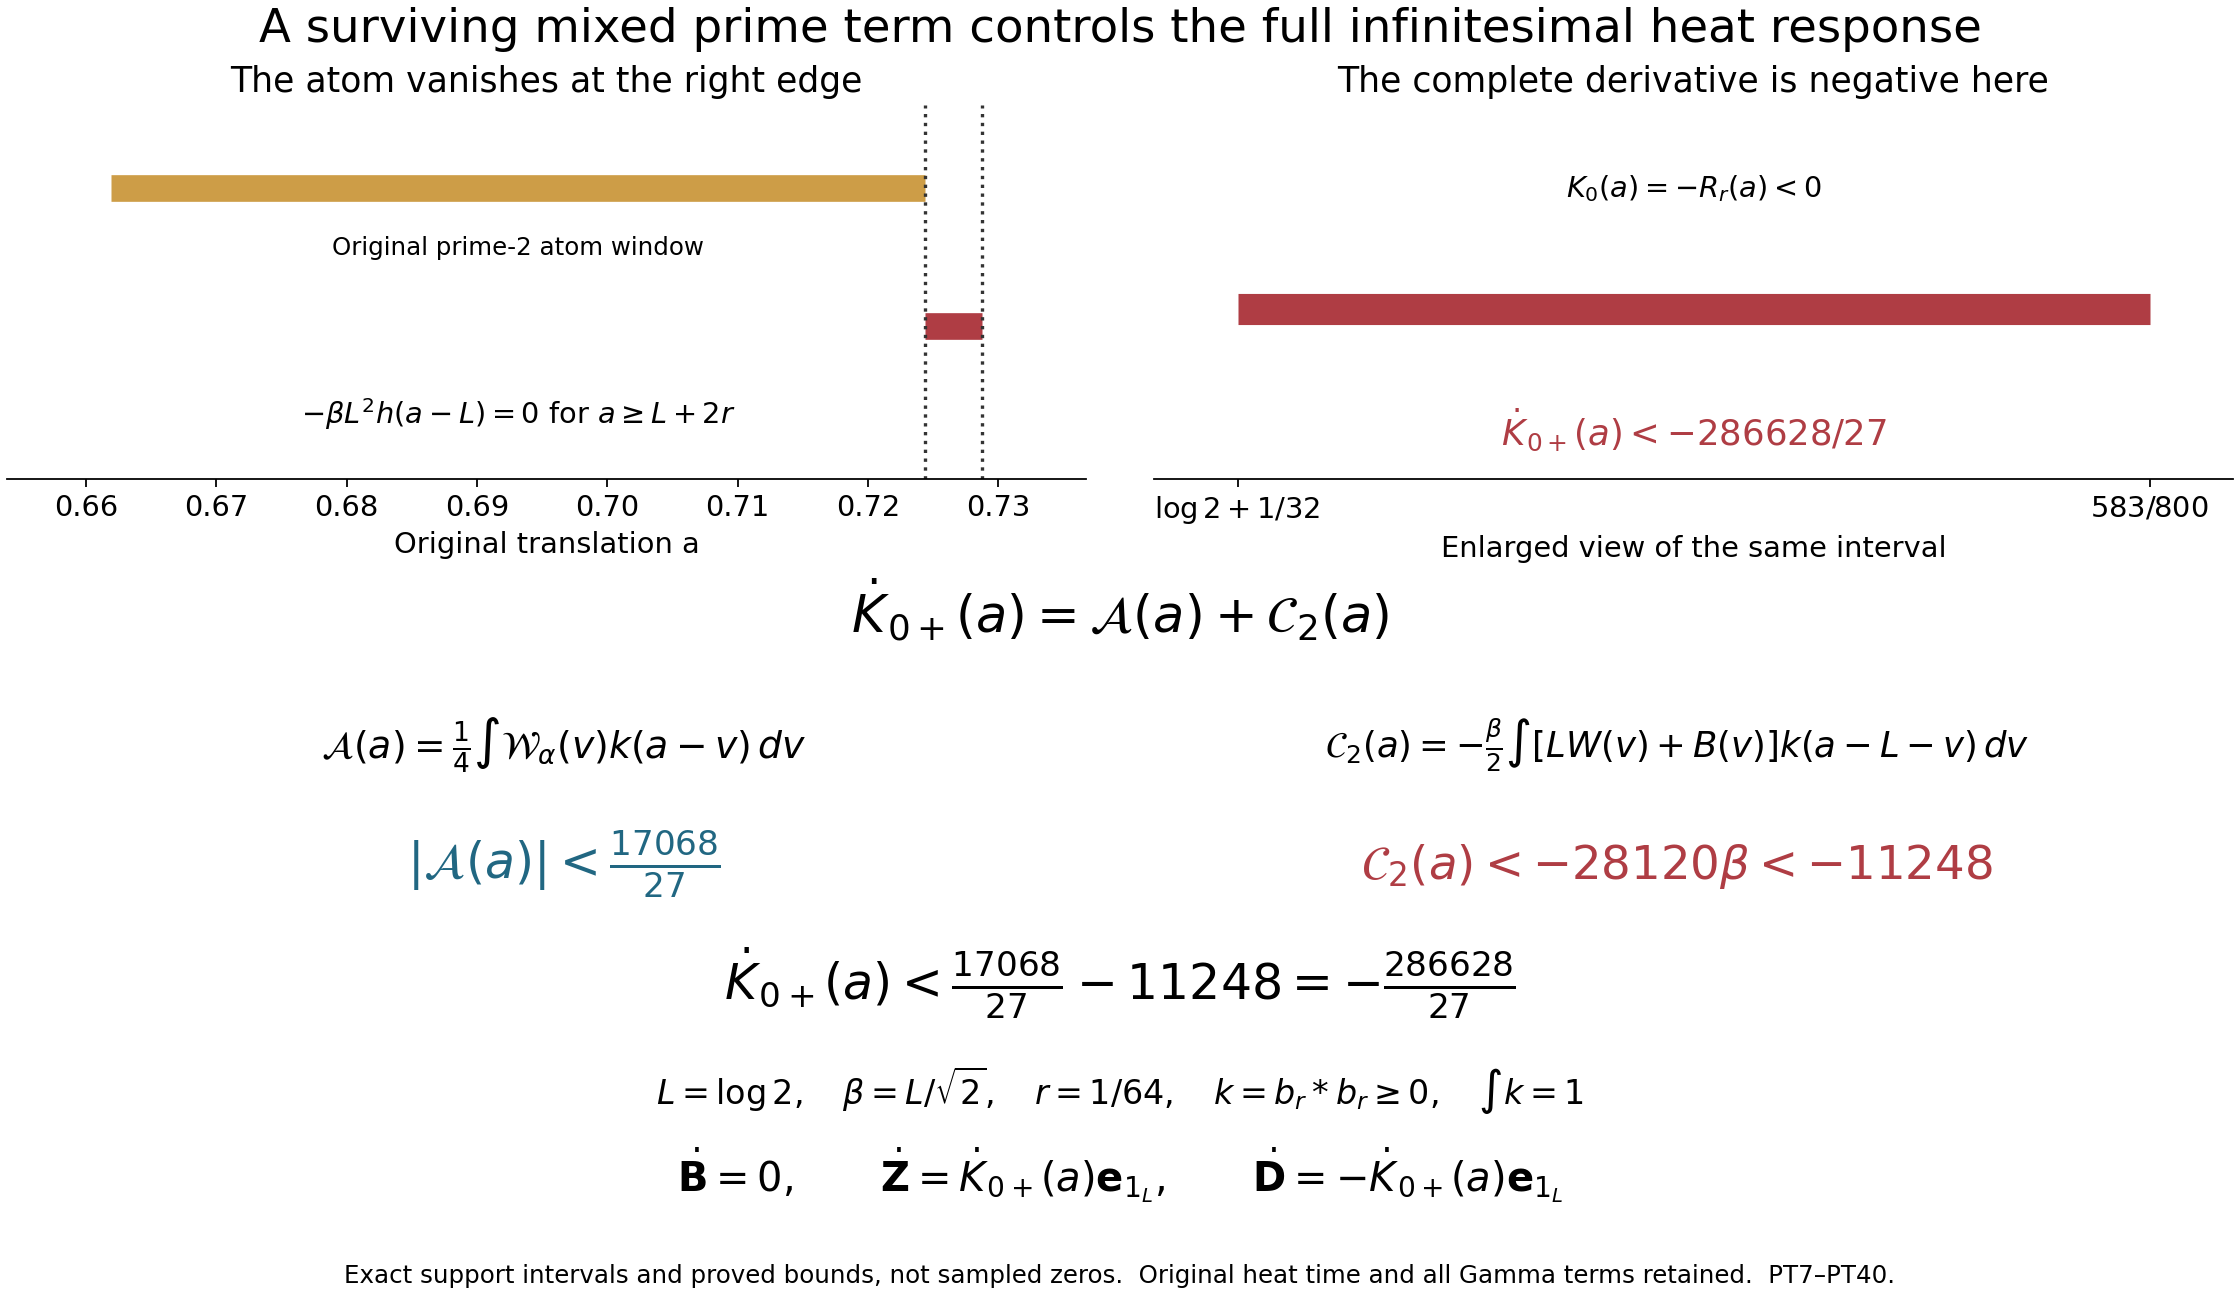
\includegraphics[keepaspectratio,alt={The original prime atom ends at log 2 plus 1/32, but its mixed heat channel remains. The enlarged interval retains the same original translation coordinates. The two displayed integral bounds include the complete archimedean convolution and the entire mixed prime-2 term; their sum proves the actual negative right derivative. The figure records rigorous inequalities, not sampled zero motion. Proofs PT7--40; actual heat differentiability RT12--16, with the original Rodgers--Tao and de Bruijn--Dobner inputs cited there.}]{prime_two_heat_tail.png}}
\caption{The original prime atom ends at log 2 plus 1/32, but its mixed
heat channel remains. The enlarged interval retains the same original
translation coordinates. The two displayed integral bounds include the
complete archimedean convolution and the entire mixed prime-2 term;
their sum proves the actual negative right derivative. The figure
records rigorous inequalities, not sampled zero motion. Proofs PT7--40;
actual heat differentiability RT12--16, with the original Rodgers--Tao
and de Bruijn--Dobner inputs cited there.}
\end{figure}

\clearpage

\section{The original fixed-test inequality through log
256}\label{the-original-fixed-test-inequality-through-log-256}

\textbf{Original-zeta receiving calculation.} The working meromorphic
function is the original Riemann zeta, with its full Gamma/endpoints
multiplier and its full trivial-zero and pole divisor retained.
\href{FAITHFUL_THETA_COMPLETION_RETURN.md}{TF1--42} proves the original
labelled theta inverse and the actual heat-image defect.
\href{FAITHFUL_UNCOMPLETED_ZETA_HEAT.md}{UZ1--53} proves every
exceptional-point fibre, jet, original-zeta heat term and reflection
orientation.
\href{ORIGINAL_ZETA_COMPACT_WEIL_RECONSTRUCTION.md}{OZC1--48} rederives
the compact contour and interval operator directly from zeta, including
the left-cutoff Gamma boundary, and specifies exactly which compensated
pairing the bounds concern.
\href{ORIGINAL_ZETA_HEAT_CONTACT_RECONSTRUCTION.md}{OZH1--49} rederives
the actual meromorphic heat, rational signed trace, compact-test domain,
contact drift and full causal arithmetic variation. The raw full divisor
and the compensated Weil receiver are linked by their displayed
correction, not identified. In particular the fixed-test trivial-zero
sum converges exactly at translations at least 1/32 and equals the
earlier R term; at zero translation it requires the proved cutoff
compensation. \href{ORIGINAL_ZETA_CAUCHY_RECONSTRUCTION.md}{OZK1--38}
reconstructs the original signed Cauchy trace, its full Gamma
correction, resonant finite parts, every finite matrix and its index,
and the complete local heat jets. Its invertible map retains the raw
trace and correction separately. These complete receiving proofs govern
the interpretation of the retained auxiliary calculations below.

Date: 23 September 2026.

For the unchanged fixed primitive test of UP and PW, the actual
correlation satisfies \[
 |K(a)|<q\qquad(0<a\le\log256),\qquad K(0)=q.
 \tag{FP1}
\] On the part extending the earlier first-prime interval, the
quantitative bound is \[
 \boxed{\displaystyle
 |K(a)|<
 \left(\frac{223}{125}+2^{-24}\right)N
 <q-\left(\frac{182}{125}-2^{-24}\right)N,
 \qquad \frac{583}{800}\le a\le\log256.}
 \tag{FP2}
\] Here \(N=\|f_r\|_2^2\), and the constant subtracted from \(q\) is
positive. The statement uses the complete original arithmetic formula,
including every prime power in each actual window and the entire
Archimedean term. It proves the stated finite interval of the existing
criterion; it makes no assertion that the inequality holds for all
translations.

\subsection{1. Original objects and source
identity}\label{original-objects-and-source-identity}

Keep \[
 r=\frac1{64},\quad t=2r=\frac1{32},\quad
 b_r=\mathop{*}_{j\ge1}
      \frac{\mathbf1_{[-r2^{-j},\,r2^{-j}]}}{2r2^{-j}},
 \quad f_r=(\partial_v^2-\tfrac14)b_r.
 \tag{FP3}
\] The construction, smoothness, support and probability mass of \(b_r\)
are proved in
\href{UNIVERSAL_PRIMITIVE_TRANSLATION_CRITERION.md}{UP1--14} and
\href{PRIMITIVE_PRIME_WINDOW_DERIVATION.md}{PW3--5}. Thus \(b_r,f_r\)
are real, even and smooth, supported in \([-r,r]\); \(b_r\ge0\) and
\(\int b_r=1\). The original Mellin transform and full pairing are \[
 M_F(s)=\int_{\mathbb R}F(v)e^{-(s-1/2)v}\,dv,\qquad
 B(F,G)=\sum_\rho m_\rho
       \overline{M_F(1-\bar\rho)}M_G(\rho).
 \tag{FP4}
\] The sum retains all actual nontrivial zeros and their actual
multiplicities. Its absolute convergence and original supported explicit
formula are in PW1--2. Set \[
 f_a(v)=f_r(v-a),\quad K(a)=B(f_a,f_r),\quad
 q=K(0),\quad N=\|f_r\|_2^2,\quad
 k_r=b_r*b_r,\quad h_r=f_r*f_r.
 \tag{FP5}
\] The functions \(k_r,h_r\) have support in \([-t,t]\); \(k_r\ge0\),
\(\int k_r=1\), and \(h_r(0)=N\). The two endpoint moments of \(f_r\)
and every translate are exactly zero because
\(M_{f_r}(s)=s(s-1)G_r(s-1/2)\). No endpoint term is discarded without
this evaluation.

The previously established ingredients read and used here are:

\begin{itemize}
\tightlist
\item
  \href{FIRST_PRIME_FULL_WEIL_COERCIVITY.md}{FC14 and FC20--FC32}: the
  exact interval operator, global-moment Legendre estimate and rational
  remainder. The read source hash is
  \texttt{30C8B05E\allowbreak{}6AC0C170\allowbreak{}95833977\allowbreak{}10F7913E\allowbreak{}D30C34D3\allowbreak{}1CE9BCD0\allowbreak{}3645A77C\allowbreak{}D3757D28}.
\item
  \href{PRIMITIVE_PRIME_WINDOW_DERIVATION.md}{PW1--PW22}: the fixed
  test, complete prime-window formula and original support maps. The
  read source hash is
  \texttt{D12B63FE\allowbreak{}28990741\allowbreak{}FBB05EFE\allowbreak{}36E07A59\allowbreak{}B4A84D88\allowbreak{}F2E205E1\allowbreak{}48038CB2\allowbreak{}9829F7D0}.
\item
  \href{FIRST_PRIME_WINDOW_BOUND.md}{FW1--FW18}: strict inequality on
  \(0<a\le583/800\), including the whole first-prime window. The read
  source hash is
  \texttt{2B3A5A88\allowbreak{}D83235C5\allowbreak{}D45B3A1A\allowbreak{}9697A07F\allowbreak{}4C2DD147\allowbreak{}969EB59B\allowbreak{}4CBA66F8\allowbreak{}CFDE5372}.
\end{itemize}

The source of the compact-interval operator and packet calculations is
the incoming \emph{Direct RH continuation: the optimal packet cost in
the full Weil form}, SHA-256
\texttt{D3B1AC08\allowbreak{}C71F6104\allowbreak{}CFE011BA\allowbreak{}5E5B86F6\allowbreak{}FBE18291\allowbreak{}6C0B0270\allowbreak{}511671B1\allowbreak{}F7165D5B}.
The present continuation uses its interval operator through the complete
FC derivation. No finite zero scan or unspecified sign of a residual
form is an input.

\subsection{2. A stronger diagonal bound at the original
radius}\label{a-stronger-diagonal-bound-at-the-original-radius}

The exact interval formula in FC14 is valid at logarithmic length
\(T_0=t=1/32\). There is no finite-prime term on this one interval:
\(T_0<\log2\). Its Archimedean operator, after the original unitary
change of coordinates, is \[
 \mathcal L+v-\log(\pi T_0)-\gamma_E-\mathcal R_{T_0},
 \qquad v(x)=-\frac12\log(1-x^2)\ge0.
 \tag{FP6}
\] The global endpoint equations become
\(\int_{-1}^1g(x)e^{\pm T_0x/4}\,dx=0\), where
\(g(x)=\sqrt{T_0/2}\,f_r(T_0x/2)\). Its squared \(L^2\) norm is still
\(N\).

Let \(c_n\) be the normalized Legendre coefficients of \(g\). The exact
eigenvalues of \(\mathcal L\) are the harmonic numbers \(H_n\);
equivalently its positive integral form and finite Legendre projections
give \[
 \langle g,\mathcal Lg\rangle
 \ge\frac32\|g\|_2^2-\frac32|c_0|^2-\frac12|c_1|^2.
 \tag{FP7}
\] This follows by integration of
\(\mathcal Lx^n=H_nx^n-\sum_{j=1}^{\lfloor n/2\rfloor}x^{n-2j}/(2j)\),
then symmetry and the degree filtration; \(H_n\ge3/2\) for \(n\ge2\).
The two global equations imply orthogonality of the even part to
\(\cosh(T_0x/4)\) and of the odd part to \(\sinh(T_0x/4)\). Taylor's
integral remainder and Cauchy--Schwarz give \[
 |c_0|^2\le A(T_0)\|g_{\mathrm{even}}\|^2,\qquad
 |c_1|^2\le\frac5{21}A(T_0)\|g_{\mathrm{odd}}\|^2,
 \quad A(T)=\frac{(T/4)^4\cosh^2(T/4)}{20}.
 \tag{FP8}
\] The constants use exactly \(\int_{-1}^1x^4\,dx=2/5\) and
\(\int_{-1}^1x^6\,dx=2/7\). The constant \(1/4\) part of the actual
kernel remainder contributes \((T_0/4)|c_0|^2\). The nonconstant part
has norm at most \(T_0E(T_0)\), where the proved FC25--28 function is \[
 \begin{gathered}
 E(T)=\sum_{j=1}^8|b_j|T^j+
          \frac{2(T/2)^9}{1-T/2},\\
 (b_1,\ldots,b_8)=
 \left(-\frac1{48},-\frac1{32},\frac7{11520},
 \frac5{1536},-\frac{31}{1935360},-\frac{61}{184320},
 \frac{127}{309657600},\frac{277}{8257536}\right).
 \end{gathered}
 \tag{FP9}
\] Those coefficients are from \(e^{z/2}/(2\sinh z)-(2z)^{-1}\);
Cauchy's bound \(2\) on \(|z|=2\) gives the displayed geometric tail.

Keeping \(v\ge0\), these estimates prove anew at this small width \[
 q\ge\left[
 \frac32+\log\frac{32}{\pi}-\gamma_E
 -T_0E(T_0)-\left(\frac32+\frac{T_0}{4}\right)A(T_0)
 \right]N.
 \tag{FP10}
\] This does not substitute a small width into FC29's separately stated
first-prime width range: FP6--FP9 prove FP10 directly, because at the
present width all finite-prime terms vanish and \(v\ge0\).

Every scalar estimate in the following evaluation is rational. The
series for cosh gives \(\cosh(T/4)\le(1-T^2/32)^{-1}\); hence, with \[
 A_+(T)=\frac{(T/4)^4}{20(1-T^2/32)^2},
\] exact substitution gives \[
 \begin{aligned}
 \Delta_0
 &:=
 T_0E(T_0)+\left(\frac32+\frac{T_0}{4}\right)A_+(T_0)\\
 &=\frac{71188529564304798199252001}
         {3342234102951354835992890572800}
 <\frac1{40000}.
 \end{aligned}
 \tag{FP11}
\] The positive integral \[
 \frac{22}{7}-\pi=\int_0^1\frac{x^4(1-x)^4}{1+x^2}\,dx
\] shows \(32/\pi>112/11\). For \(z=23201/10000\), the exact positive
Taylor bound \[
 e^z\le
 \sum_{j=0}^{16}\frac{z^j}{j!}
 +\frac{z^{17}}{17!}\frac1{1-z/18}
 <\frac{112}{11}
 \tag{FP12}
\] therefore proves \(\log(32/\pi)>23201/10000\). The tail inequality
follows because every successive omitted-term ratio is at most
\(z/18<1\). The second inequality is an exact rational comparison,
reproduced by the accompanying checker. Finally \[
 \gamma_E<H_{256}-8\log2
 <H_{256}
   -16\sum_{j=0}^3\frac1{(2j+1)3^{2j+1}}
 <\frac{29}{50}.
 \tag{FP13}
\] The first inequality follows from the decreasing sequence
\(H_n-\log n\); the second from the positive integrated geometric series
for \(\log2\); the last is a finite rational sum. Equations FP10--FP13
give the stronger explicit diagonal estimate \[
 \boxed{\displaystyle
 q>\frac{129603}{40000}N>\frac{81}{25}N>3N.}
 \tag{FP14}
\] The function \(f_r\) is nonzero, so these strict inequalities have
their asserted nonzero norm.

\subsection{3. A compact-support mass estimate for the actual
density}\label{a-compact-support-mass-estimate-for-the-actual-density}

Twice integrating by parts, with all derivatives of \(b_r\) zero at its
support endpoints, gives the exact identity \[
 N=\|b_r''\|_2^2+\frac12\|b_r'\|_2^2+\frac1{16}\|b_r\|_2^2.
 \tag{FP15}
\] For any smooth compact density \(b\) on \([-r,r]\) of integral one,
let \(\phi(x)=(r^2-x^2)^2\). Integration by parts yields \[
 \int_{-r}^r b''(x)\phi''(x)\,dx=24,\qquad
 \|\phi''\|_2^2=\frac{128r^5}{5}.
\] Cauchy--Schwarz gives \(\|b''\|_2^2\ge45/(2r^5)\). This leading
derivative constant is sharp in the clamped Sobolev space:
\(b(x)=15(r^2-x^2)^2/(16r^5)\) has integral one, has zero value and
derivative at both endpoints, and attains equality. No claim that this
polynomial is the actual smooth infinite convolution is made.

The further identities \(\int xb'=-1\) and \(\int b=1\) give \[
 \|b'\|_2^2\ge\frac3{2r^3},\qquad
 \|b\|_2^2\ge\frac1{2r}.
\] The last inequality is strict for a nonzero compact smooth density:
equality would make it constant almost everywhere on the interval,
contradicting continuity and its zero endpoint values. Substituting into
FP15 yields, for the unchanged \(r=1/64\), \[
 \boxed{\displaystyle
 N>\frac{45}{2r^5}+\frac3{4r^3}+\frac1{32r}
   =24159387650.}
 \tag{FP16}
\] The three separate lower bounds are not claimed to be jointly
attained. They prove exactly the stated lower bound for this actual
\(N\).

\subsection{4. The complete arithmetic window and the Archimedean
estimate}\label{the-complete-arithmetic-window-and-the-archimedean-estimate}

For \(a>t\), the exact PW13--PW17 expression is \[
 K(a)=-R(a)-
       \sum_{\substack{n\ge2\\|\log n-a|\le t}}
         \frac{\Lambda(n)}{\sqrt n}h_r(a-\log n),
 \quad
 R(a)=\int_{a-t}^{a+t}W(v)k_r(a-v)\,dv,
 \tag{FP17}
\] \[
 W(v)=
 \frac{4e^{-5v/2}(9+55e^{-2v}+31e^{-4v}+e^{-6v})}
      {(1-e^{-2v})^5}>0.
 \tag{FP18}
\] This is the full Archimedean cross term after four integrations by
parts using \(h_r=(\partial_v^2-\tfrac14)^2k_r\), with its negative sign
in FP17. All boundary terms vanish because \(k_r\) is smooth and
supported in \([-t,t]\). The expansion \[
 W(v)=\sum_{j\ge1}4j^2(2j+1)^2e^{-(2j+1/2)v}
\] shows that \(W\) is strictly decreasing. Since \(k_r\) is a
probability density, \(0<R(a)\le W(a-t)\).

Put \(A_*=583/800\). For every \(a\ge A_*\), \(a-t\ge279/400>2/3\). The
first three positive terms of \(e^{4/3}\) already exceed three, so
\(e^{-2v}<1/3\) for \(v\ge2/3\). Bounding \(e^{-5v/2}<1\) in the actual
positive formula FP18 gives \[
 W(v)<
 \frac{4(9+55/3+31/9+1/27)}{(1-1/3)^5}=936.
\] Together with FP16 this proves the entire, untruncated remainder
bound \[
 \boxed{\displaystyle 0<R(a)<936<2^{-24}N
                       \qquad(a\ge583/800).}
 \tag{FP19}
\] The final comparison is the integer inequality
\(936\cdot2^{24}<24159387650\).

\subsection{5. Every prime power in the bounded translation
interval}\label{every-prime-power-in-the-bounded-translation-interval}

Haar Cauchy--Schwarz gives \(|h_r(u)|\le N\) for every real \(u\). Thus
FP17 implies \[
 |K(a)|\le R(a)+N S(a),\qquad
 S(a)=\sum_{\substack{n\ge2\\|\log n-a|\le1/32}}
                  \frac{\Lambda(n)}{\sqrt n}.
 \tag{FP20}
\] The finite coefficient certificate FPC1--FPC14, proved in
\url{FINITE_PRIME_WINDOW_COEFFICIENT_CERTIFICATE.md} establishes \[
 \boxed{\displaystyle S(a)<\frac{223}{125}
            \qquad(583/800\le a\le\log256).}
 \tag{FP21}
\] This lemma retains every prime power. In particular, the upper end of
the actual window can exceed \(256\): \[
 n\le256e^{1/32}
 <256(1-1/32)^{-1}=\frac{8192}{31}<265.
 \tag{FP22}
\] The required list therefore includes \(257\) and \(263\), and
contains every prime power at most \(264\). The proof does not truncate
the arithmetic expression at \(256\). Every simultaneous window packet
has largest index divided by its smallest index at most
\(e^{1/16}<16/15\). The certificate enumerates the complete maximal
packets for this slightly larger rational ratio and bounds every
coefficient by rational logarithm and square-root estimates. Its largest
packet is \(\{227,229,233,239,241\}\), and its bound is below
\(223/125\). This packet also fits the original window, since
\(\log(241/227)<14/227<1/16\); the certificate's check is not based on
unrelated equally spaced translations.

At a support edge, \(h_r(\pm1/32)=0\), with all its derivatives zero.
Using the closed inequality in the window condition merely retains the
corresponding evaluated zero term. No edge term or supported coordinate
is lost.

\subsection{6. Combine the estimates without changing the
criterion}\label{combine-the-estimates-without-changing-the-criterion}

For \(A_*\le a\le\log256\), FP19--FP21 give \[
 |K(a)|<
 \left(\frac{223}{125}+2^{-24}\right)N.
\] FP14 gives \[
 \left(\frac{223}{125}+2^{-24}\right)N
 <q-\left(\frac{182}{125}-2^{-24}\right)N,
\] which is FP2. The exact rational margin is \[
 \frac{182}{125}-2^{-24}
       =\frac{3053453187}{2097152000}>\frac75.
 \tag{FP23}
\] Both signs of the actual two-test form are therefore strictly
positive with that margin: \[
 Q(f_r+f_a)=2q+2K(a)>
       2\left(\frac{182}{125}-2^{-24}\right)N,\qquad
 Q(f_r-f_a)=2q-2K(a)>
       2\left(\frac{182}{125}-2^{-24}\right)N.
 \tag{FP24}
\]

On \(0<a\le A_*\), FW8--FW9 already give the strict inequality. Its
proof uses the full FC coercivity theorem on the union of the two
translated supports, of containing length at most \(a+1/32\). The
two-by-two Gram bound is \[
 |K(a)-c_*h_r(a)|<q-c_*N,\qquad
 c_*=\frac{11509}{600000}.
\] Together with \(|h_r(a)|\le N\) it gives \(|K(a)|<q\). This covers
the remaining interval, including the overlapping-support case near
zero; at zero the exact value is \(K(0)=q\). Combining that result with
FP2 proves FP1 through the requested endpoint \(\log256\).

The original criterion is still precisely PW11/PW20, involving this same
\(K,q,b_r,f_r\) and all real \(a\ge0\). The present result proves its
required inequality for a larger, explicit finite interval. It neither
substitutes another test family nor concludes that the remaining
translations satisfy it.

\subsection{7. Original supported-zero maps and reproducible
arithmetic}\label{original-supported-zero-maps-and-reproducible-arithmetic}

All observations and translations retain the original fixed-carrier map
\((v,\lambda)\mapsto(Av,\lambda)\). In particular the endpoint-zero
moment is the supported value \((0,1_L)\), not \(\tau=(0,0_L)\), for a
top-supported input. The full trace vector remains exactly PW21: \[
 \boldsymbol B_L(a)=0,\quad
 \boldsymbol Z_L(a)=K(a)\mathbf e_{1_L},\quad
 \boldsymbol D_L(a)=-K(a)\mathbf e_{1_L}.
 \tag{FP25}
\] The lifted pairing is \[
 B^L((u,\lambda),(v,\mu))=(B(u,v),\lambda\wedge\mu).
\] Applying the amplitude estimate FP2 leaves every coefficient space,
endpoint label and support map present. The estimates bound the actual
top amplitude after the existing receiver; they do not identify
supported vanishing with absence or add a different prime weight at the
endpoint.

\url{finite_prime_window_extension_check.py} reproduces FP11--FP16,
FP19, FP22 and FP23 using exact rational arithmetic. The independent
coefficient certificate and its checker reproduce the complete
finite-prime lemma FP21. No calculation uses floating zeta-zero samples
or a numerical approximation to the infinite convolution. The profile
enters through its proved smoothness, exact support, total mass,
original moments and exact autocorrelation formula.

\subsection{Exact objects and proved
bounds}\label{exact-objects-and-proved-bounds-2}

\begin{figure}
\centering
\pandocbounded{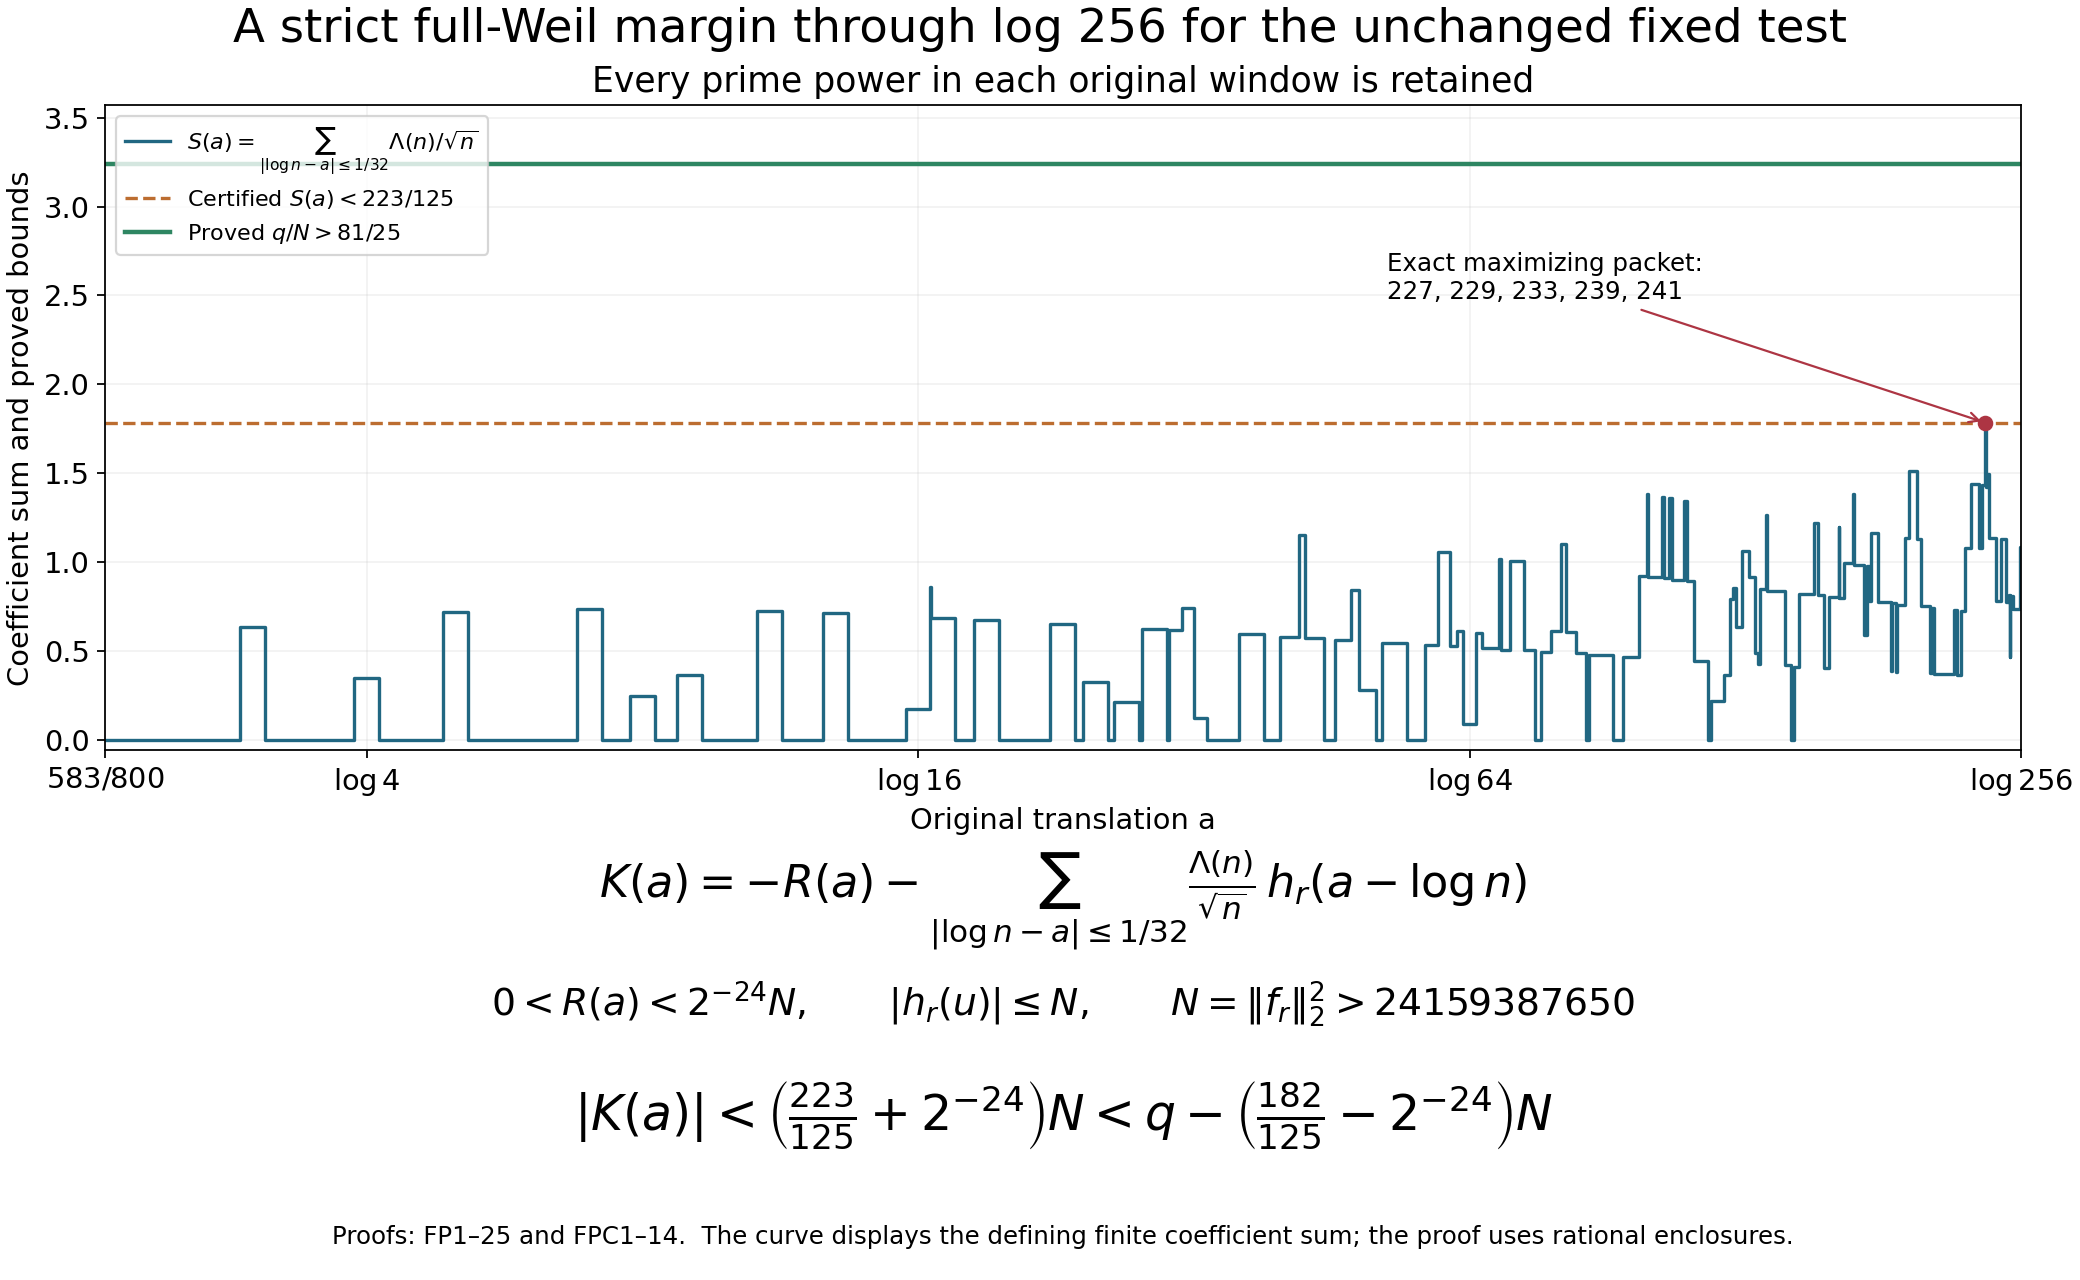
\includegraphics[keepaspectratio,alt={The complete coefficient sum in the original arithmetic window and the proved bounds for the unchanged test. The plotted step function is rendered from its defining natural logarithms and prime-power weights; FPC1--14 proves its bound and exact maximizing packet using rational enclosures, with all 72 prime powers through 264 retained. FP6--24 bounds the full archimedean term and diagonal before combining them. The profile keeps the classical Arias density, radius 1/64 and original endpoint filter. No zero sampling enters the proof.}]{finite_prime_bound.png}}
\caption{The complete coefficient sum in the original arithmetic window
and the proved bounds for the unchanged test. The plotted step function
is rendered from its defining natural logarithms and prime-power
weights; FPC1--14 proves its bound and exact maximizing packet using
rational enclosures, with all 72 prime powers through 264 retained.
FP6--24 bounds the full archimedean term and diagonal before combining
them. The profile keeps the classical Arias density, radius 1/64 and
original endpoint filter. No zero sampling enters the proof.}
\end{figure}

\clearpage

\section{Exact coefficient bound for the original prime-power
window}\label{exact-coefficient-bound-for-the-original-prime-power-window}

For the original von Mangoldt function, including every prime power,
define \[
S(a)=\sum_{\substack{n\ge2\\|\log n-a|\le1/32}}
\frac{\Lambda(n)}{\sqrt n},
\qquad \frac{583}{800}\le a\le\log256.
\tag{FPC1}
\] All logarithms are natural. The exact maximum on this entire real
interval is \[
\boxed{
\max_a S(a)=M_*:=
\frac{\log227}{\sqrt{227}}+
\frac{\log229}{\sqrt{229}}+
\frac{\log233}{\sqrt{233}}+
\frac{\log239}{\sqrt{239}}+
\frac{\log241}{\sqrt{241}}.
}
\tag{FPC2}
\] Its certified rational enclosure is \[
\frac{1783796246}{10^9}<M_*<\frac{1783796247}{10^9}
<\boxed{\frac{223}{125}}<2.
\tag{FPC3}
\] This calculation is finite arithmetic. It does not evaluate or
truncate any zeta-zero sum.

\subsection{The exact finite range and ratio
reduction}\label{the-exact-finite-range-and-ratio-reduction}

For \(0<x<1\), comparison of the exponential series with the geometric
series gives \(e^x<1/(1-x)\). Therefore \[
n\le e^{a+1/32}\le256e^{1/32}
<256\frac{32}{31}=\frac{8192}{31}<265.
\tag{FPC4}
\] Thus all contributing indices satisfy \(n\le264\). Both primes 257
and 263 must be retained. In fact \(e^{1/32}>1+1/32\) gives
\(256e^{1/32}>264\), so the exact integer upper cutoff is 264.

The first index 2 never occurs. The elementary logarithm series gives \[
\log2=2\sum_{j\ge0}\frac{(1/3)^{2j+1}}{2j+1}
<\frac23+\frac{2(1/3)^3}{3(1-1/9)}
=\frac{25}{36}<\frac{279}{400}
=\frac{583}{800}-\frac1{32}.
\tag{FPC5}
\] The strict series bound follows because each denominator after the
first term is at least 3, and those after that are strictly larger.
Non-prime-power indices have coefficient zero and are preserved with
that numerical value.

Any two indices \(m\le n\) in the same window obey \[
\frac nm\le e^{1/16}<\frac{16}{15}.
\tag{FPC6}
\] Let \(\mathcal P\) be the set of all prime powers at most 264. If a
window has a nonzero coefficient, let \(m\ge3\) be its smallest
contributing prime power. Its contribution is bounded above by the full
positive sum on the exact rational superset \[
U_m=\{n\in\mathcal P:m\le n,\ 15n<16m\}.
\tag{FPC7}
\] This leaves exactly 71 cases, one for each member of
\(\mathcal P\setminus\{2\}\). A window containing no prime power has
value zero.

\subsection{Rational bounds for every individual
weight}\label{rational-bounds-for-every-individual-weight}

The companion checker uses integer arithmetic, exact fractions, and
integer square roots. It uses no floating-point value of a logarithm,
exponential, square root, or zero of zeta.

For \(0\le z\le1/3\), integrating a finite geometric expansion of
\(2/(1-z^2)\) proves \[
L_N(z):=2\sum_{j=0}^{N-1}\frac{z^{2j+1}}{2j+1}
\le \log\frac{1+z}{1-z}
\le L_N(z)+\frac{2z^{2N+1}}{(2N+1)(1-z^2)}.
\tag{FPC8}
\] Use \(N=16\). For an integer prime \(p\), put
\(k=\lfloor\log_2p\rfloor\), evaluated by its integer bit length, and \[
z_p=\frac{p-2^k}{p+2^k}\in[0,1/3).
\] Then \[
\log p=k\log2+\log\frac{1+z_p}{1-z_p}.
\tag{FPC9}
\] Apply FPC8 to both logarithms, and round the lower bound down and the
upper bound up to denominator \(10^{12}\). Denote the resulting rational
bounds by \(\lambda_p^-\) and \(\lambda_p^+\).

For each prime power \(n=p^j\), compute the integer \[
b_n=\operatorname{isqrt}(n\,10^{18}).
\] Set \(r_n^-=b_n/10^9\). If \(b_n^2=n10^{18}\), set \(r_n^+=r_n^-\);
otherwise set \(r_n^+=(b_n+1)/10^9\). By the defining
integer-square-root inequalities, \[
(r_n^-)^2\le n\le(r_n^+)^2,
\qquad
\frac{\lambda_p^-}{r_n^+}
\le\frac{\Lambda(n)}{\sqrt n}
\le\frac{\lambda_p^+}{r_n^-}.
\tag{FPC10}
\] Every denominator is positive. The checker records all 72 prime-power
indices, their prime bases, and all six rational log, square-root, and
weight bounds in the accompanying JSON.

The enumeration itself is exhaustive: trial division through the integer
square root decides every prime \(p\le264\), and repeated integer
multiplication generates every \(p^j\le264\). Every prime power has
exactly one such prime base. The complete resulting set has 72 members,
including \(243=3^5\), \(256=2^8\), 257 and 263.

\subsection{The complete finite comparison and
attainment}\label{the-complete-finite-comparison-and-attainment}

Adding the upper bounds in FPC10 on each exact set FPC7 yields the
following certified comparisons: \[
\sum_{n\in U_m}\frac{\Lambda(n)}{\sqrt n}
<\frac{1511}{1000}\quad(m\ne227),
\tag{FPC11}
\] whereas \[
U_{227}=\{227,229,233,239,241\},
\quad
\frac{1783796246}{10^9}<M_*<\frac{1783796247}{10^9}.
\tag{FPC12}
\] The lower bound in FPC12 exceeds \(1511/1000\), so this proves the
maximum over all 71 supersets exactly. These are exact rational
comparisons, not decimal estimates. Their full fractions and all
constituent indices are provided in the JSON. The full 71-case table
displays each packet and an outward-rounded upper bound with denominator
\(10^9\).

Selected packet bounds, including the packet containing 257 and 263, are

{\def\LTcaptype{none} % do not increment counter
\begin{longtable}[]{@{}rlr@{}}
\toprule\noalign{}
Minimum & Complete ratio packet & Certified upper bound \\
\midrule\noalign{}
\endhead
\bottomrule\noalign{}
\endlastfoot
227 & 227, 229, 233, 239, 241 & \(1783796247/10^9\) \\
191 & 191, 193, 197, 199 & \(1510503007/10^9\) \\
229 & 229, 233, 239, 241, 243 & \(1494205679/10^9\) \\
251 & 251, 256, 257, 263 & \(1081820789/10^9\) \\
\end{longtable}
}

The superset maximum occurs in an actual window of the original width.
Choose \[
a_*^{\rm win}=\frac{\log227+\log241}{2}.
\tag{FPC13}
\] For every prime in the displayed five-prime packet, \[
|\log p-a_*^{\rm win}|
\le\frac12\log\frac{241}{227}
<\frac12\frac{14}{227}<\frac1{32}.
\tag{FPC14}
\] Here \(\log(1+x)<x\), and \(224<227\) proves the final rational
inequality. Also \(227\cdot241<256^2\), so \(a_*^{\rm win}<\log256\).
For the lower endpoint, \(\log227>\log4=2\log2>4/3>583/800\), using the
first positive term of the logarithm series. Thus FPC13 is admissible.
Its window contains the whole five-prime packet, while FPC11--FPC12
already exclude any larger sum. It attains exactly \(M_*\), proving FPC2
and the uniform bound FPC3.

\subsection{Reproduction files}\label{reproduction-files}

\begin{itemize}
\tightlist
\item
  \texttt{check\_\allowbreak{}finite\_\allowbreak{}prime\_\allowbreak{}window\_\allowbreak{}coefficients.\allowbreak{}py}: the complete
  rational-only enumeration and all asserted comparisons.
\item
  \texttt{FINITE\_\allowbreak{}PRIME\_\allowbreak{}WINDOW\_\allowbreak{}COEFFICIENT\_\allowbreak{}CERTIFICATE.\allowbreak{}json}: every
  individual rational enclosure and every one of the 71 packet sums.
\item
  \texttt{FINITE\_\allowbreak{}PRIME\_\allowbreak{}WINDOW\_\allowbreak{}PACKETS.\allowbreak{}md}: the complete
  human-readable packet table, with rational upper bounds.
\end{itemize}

Run the Python checker in this directory. It reproduces the JSON and the
complete packet table, and fails if any stated comparison fails. The
exact maximum is the symbolic sum FPC2; its rational enclosure is FPC3.
No source window, prime-power coefficient, or endpoint has been
replaced.

\section{Exact rational packet table}\label{exact-rational-packet-table}

Each upper bound is the displayed integer divided by \(10^9\). It is an
outward rounding of the exact upper fraction in the companion JSON.

{\def\LTcaptype{none} % do not increment counter
\begin{longtable}[]{@{}
  >{\raggedleft\arraybackslash}p{(\linewidth - 4\tabcolsep) * \real{0.3333}}
  >{\raggedright\arraybackslash}p{(\linewidth - 4\tabcolsep) * \real{0.3333}}
  >{\raggedleft\arraybackslash}p{(\linewidth - 4\tabcolsep) * \real{0.3333}}@{}}
\toprule\noalign{}
\begin{minipage}[b]{\linewidth}\raggedleft
Minimum prime power
\end{minipage} & \begin{minipage}[b]{\linewidth}\raggedright
All prime powers in its ratio superset
\end{minipage} & \begin{minipage}[b]{\linewidth}\raggedleft
Upper numerator over \(10^9\)
\end{minipage} \\
\midrule\noalign{}
\endhead
\bottomrule\noalign{}
\endlastfoot
3 & 3 & 634284101 \\
4 & 4 & 346573591 \\
5 & 5 & 719762516 \\
7 & 7 & 735484905 \\
8 & 8 & 245064536 \\
9 & 9 & 366204097 \\
11 & 11 & 722992628 \\
13 & 13 & 711388957 \\
16 & 16, 17 & 860441965 \\
17 & 17 & 687155170 \\
19 & 19 & 675500630 \\
23 & 23 & 653795740 \\
25 & 25 & 321887583 \\
27 & 27 & 211428034 \\
29 & 29 & 625291138 \\
31 & 31, 32 & 739294578 \\
32 & 32 & 122532268 \\
37 & 37 & 593631249 \\
41 & 41, 43 & 1153540161 \\
43 & 43 & 573577641 \\
47 & 47, 49 & 839588912 \\
49 & 49 & 277987165 \\
53 & 53 & 545361537 \\
59 & 59, 61 & 1057193623 \\
61 & 61, 64 & 612986861 \\
64 & 64, 67 & 600328359 \\
67 & 67, 71 & 1019571991 \\
71 & 71, 73 & 1008047325 \\
73 & 73 & 502160296 \\
79 & 79, 81, 83 & 1098700093 \\
81 & 81, 83 & 607098802 \\
83 & 83 & 485030770 \\
89 & 89 & 475794504 \\
97 & 97, 101, 103 & 1380386597 \\
101 & 101, 103, 107 & 1367634487 \\
103 & 103, 107, 109 & 1357762463 \\
107 & 107, 109, 113 & 1345804284 \\
109 & 109, 113 & 894064869 \\
113 & 113 & 444715238 \\
121 & 121, 125, 127, 128 & 853061211 \\
125 & 125, 127, 128, 131 & 1061018700 \\
127 & 127, 128, 131 & 917066197 \\
128 & 128, 131 & 487214102 \\
131 & 131, 137, 139 & 1264826923 \\
137 & 137, 139 & 838878955 \\
139 & 139 & 418536617 \\
149 & 149, 151, 157 & 1221772044 \\
151 & 151, 157 & 811832789 \\
157 & 157, 163, 167 & 1198547906 \\
163 & 163, 167, 169, 173 & 1384116861 \\
167 & 167, 169, 173 & 985143554 \\
169 & 169, 173, 179 & 976824721 \\
173 & 173, 179, 181 & 1165922166 \\
179 & 179, 181 & 774124661 \\
181 & 181, 191, 193 & 1145259138 \\
191 & 191, 193, 197, 199 & 1510503007 \\
193 & 193, 197, 199 & 1130461840 \\
197 & 197, 199 & 751645111 \\
199 & 199, 211 & 743669539 \\
211 & 211, 223 & 730528112 \\
223 & 223, 227, 229, 233 & 1438337443 \\
227 & 227, 229, 233, 239, 241 & 1783796247 \\
229 & 229, 233, 239, 241, 243 & 1494205679 \\
233 & 233, 239, 241, 243 & 1135135222 \\
239 & 239, 241, 243, 251 & 1126789316 \\
241 & 241, 243, 251, 256, 257 & 1162009892 \\
243 & 243, 251, 256, 257 & 808703063 \\
251 & 251, 256, 257, 263 & 1081820789 \\
256 & 256, 257, 263 & 733057292 \\
257 & 257, 263 & 689735593 \\
263 & 263 & 343593738 \\
\end{longtable}
}

\clearpage

\section{The original zeta function, faithful theta recovery, and the
heat return
defect}\label{the-original-zeta-function-faithful-theta-recovery-and-the-heat-return-defect}

This calculation retains the original meromorphic Riemann zeta function,
its full multiplier, the supported-zero contribution, and every lower
support coefficient. It reconstructs the theta input explicitly and
calculates the obstruction to realizing the source heat family by
another input in the same theta domain. The obstruction is then mapped
isomorphically to specified meromorphic principal parts. No assertion of
RH is used.

\subsection{1. Original carrier and exact analytic
domain}\label{original-carrier-and-exact-analytic-domain}

Let \(L\) be a finite bounded distributive lattice with distinct bottom
and top. The carrier is \[
G_L(A)=\{(a,1_L):a\in A\}\cup\{z_\lambda=(0,\lambda):\lambda\ne1_L\},
\quad e_L=(0,1_L),\quad\tau_L=(0,0_L).
\tag{TF1}
\] Addition uses amplitude addition and support join; multiplication
uses amplitude multiplication and support meet. In the two-support
integer subcarrier the principal ideals are \[
(\tau)=\{\tau\}\subsetneq(e)=\{\tau,e\}\subsetneq
(p)=\{\tau\}\cup(p\mathbb Z)^\bullet.
\tag{TF2}
\] Each is prime: an unsupported product has an unsupported factor; a
supported product has amplitude zero only if one integer factor has
amplitude zero; and divisibility by an ordinary prime is tested on the
amplitudes. This retains the prime supported zero. It does not identify
it with the unsupported element. The complete lattice and adelic carrier
maps are the retained SZW1--13 proof in
\texttt{SUPPORTED\_\allowbreak{}ZERO\_\allowbreak{}PRIME\_\allowbreak{}WEIL\_\allowbreak{}DERIVATION.\allowbreak{}md}; the present domain
is its global fixed-sector carrier, not the larger carrier with
nonconstant proper adelic strata.

Use exactly \[
\mathcal F_L=\mathcal S_{\rm ev}(\mathbb R)\oplus
\bigoplus_{\lambda\ne1_L}\mathbb C\delta_\lambda,
\qquad F=(\phi,(c_\lambda)),
\qquad \widehat\phi(y)=\int_{\mathbb R}\phi(x)e^{-2\pi ixy}\,dx.
\tag{TF3}
\] The point-functions \(\delta_\lambda\) retain separate coefficients.
They are not Dirac distributions on the real line. For \(x>0\), put \[
a=\phi(0),\quad b=\int_{\mathbb R}\phi(x)\,dx,\quad
\Theta_e\phi(x)=\sum_{n\in\mathbb Z}\phi(nx),\quad
P\phi(x)=\sum_{n\ne0}\phi(nx).
\tag{TF4}
\] The labelled sum is
\(\Theta_e\phi(x)\,\mathbf e_{1_L}+\sum_{\lambda\ne1_L}c_\lambda\mathbf e_\lambda\),
where the \(\mathbf e_\lambda\) are independent coordinates in
\(\mathbb C^L\). Its top coordinate includes the supported zero once. On
compact positive \(x\)-intervals every derivative of the sums converges
absolutely by a sufficiently high Schwartz bound. Poisson summation
gives \[
\Theta_e\phi(x)=x^{-1}\Theta_e\widehat\phi(x^{-1}),\qquad
P\phi(x)=x^{-1}P\widehat\phi(x^{-1})+b/x-a.
\tag{TF5}
\] For each lower coordinate the raw Fourier convention fixes
\(c_\lambda\); its Poisson defect is exactly \(c_\lambda(1-x^{-1})\).
These distinct defects must not be replaced by their possibly vanishing
scalar sum.

\subsection{2. Original zeta in the Mellin
calculation}\label{original-zeta-in-the-mellin-calculation}

For \(\Re s>1\), absolute convergence and the substitution \(y=nx\) give
\[
Z_\phi(s)=\int_0^\infty P\phi(x)x^{s-1}\,dx
=2\zeta(s)\mathcal M\phi(s),\qquad
\mathcal M\phi(s)=\int_0^\infty\phi(x)x^{s-1}\,dx.
\tag{TF6}
\] Here \(\zeta(s)=\sum_{n\ge1}n^{-s}\) on that half-plane. The Mellin
transform \(\mathcal M\phi\) is holomorphic on \(\Re s>0\), because
\(\phi\) is bounded near zero and has arbitrarily high decay at
infinity; the same bounds with powers of \(\log x\) justify parameter
derivatives. Splitting TF6 at one and applying TF5 gives the exact
continuation \[
Z_\phi(s)=\int_1^\infty P\phi(x)x^{s-1}\,dx
+\int_1^\infty P\widehat\phi(x)x^{-s}\,dx
+\frac{b}{s-1}-\frac{a}{s}.
\tag{TF7}
\] Both integrals are entire, by the derivative versions of the Schwartz
bounds. The residues are \(b\) at one and \(-a\) at zero. Lower fixed
coefficients have two separate tail terms \(c_\lambda/s\) and
\(-c_\lambda/s\). Their meromorphic sum is zero, while each fixed
representation has its nonzero character distribution; SZW16--18 proves
both maps. We retain \((c_\lambda)\) alongside TF6--7.

For the original Gaussian \(\phi_{\rm G}(x)=e^{-\pi x^2}\), substitution
\(y=\pi x^2\) gives \[
\mathcal M\phi_{\rm G}(s)=\frac12\pi^{-s/2}\Gamma(s/2),\quad
Z_{\phi_{\rm G}}(s)=\pi^{-s/2}\Gamma(s/2)\zeta(s).
\tag{TF8}
\] Thus the Gaussian is a specified analytic input. TF1 alone does not
select this input, its measure, or the subsequent heat operation. Its
comparison to the original zeta is TF8 with every factor retained.

\subsection{3. The exact theta filter and its
inverse}\label{the-exact-theta-filter-and-its-inverse}

Define \[
w_\phi(u)=e^u\Theta_e\phi(e^{2u}),\qquad
\Phi_\phi(u)=\frac1{16}(D_u^2-1)w_\phi(u).
\tag{TF9}
\] For every derivative order \(j\) and \(A>0\), Schwartz estimates and
TF5 prove \[
D_u^j(w_\phi-ae^u)=O_{A,j}(e^{-Au})\quad(u\to+\infty),
\qquad
D_u^j(w_\phi-be^{-u})=O_{A,j}(e^{Au})\quad(u\to-\infty).
\tag{TF10}
\] Indeed differentiating a summand introduces powers of \(ne^{2u}\),
bounded by a higher Schwartz seminorm and a convergent inverse-power sum
in \(n\). This proves the first estimate; apply the same bound to
\(\widehat\phi\) in TF5 for the second. Since \(D_u^2-1\) annihilates
both exponential terms, \(\Phi_\phi\) and all its derivatives decrease
faster than every exponential at both ends.

The endpoint coefficients are exactly recoverable: \[
a=8\int_{\mathbb R}e^{-u}\Phi_\phi(u)\,du,
\qquad b=8\int_{\mathbb R}e^u\Phi_\phi(u)\,du.
\tag{TF11}
\] To prove this, differentiate the two Wronskians: \[
\big(e^{-u}(w_\phi'+w_\phi)\big)'=16e^{-u}\Phi_\phi,
\qquad
\big(e^u(w_\phi'-w_\phi)\big)'=16e^u\Phi_\phi.
\tag{TF12}
\] The first bracket has limits zero and \(2a\), and the second has
limits \(-2b\) and zero, at the negative and positive ends respectively.
TF10 proves each limit and absolute integrability. Integration gives
TF11.

The complete inverse at the theta level is \[
\begin{aligned}
w_\phi(u)
&=a e^u+16\int_u^\infty\sinh(v-u)\Phi_\phi(v)\,dv\\
&=8\int_{\mathbb R}e^{|u-v|}\Phi_\phi(v)\,dv.
\end{aligned}
\tag{TF13}
\] For the first expression, two differentiations give
\((D_u^2-1)w=16\Phi_\phi\). Its difference from the original \(w_\phi\)
is a homogeneous solution \(Ae^u+Be^{-u}\), decreasing faster than every
exponential as \(u\to+\infty\) by TF10 and the tail estimate. Both
constants are therefore zero. The second expression follows by inserting
TF11 and splitting its integral at \(u\). No endpoint coefficient has
been assigned by an arbitrary boundary choice.

The input itself is recovered without division at a zeta zero: \[
\Theta_e\phi(x)=x^{-1/2}w_\phi(\tfrac12\log x),\qquad
\phi(x)=\frac12\sum_{n\ge1}\mu(n)
\big(\Theta_e\phi(nx)-a\big),\quad x>0.
\tag{TF14}
\] Substituting TF4 gives \(\sum_{n,k\ge1}\mu(n)\phi(knx)\). Its
absolute sum is at most \(\sum_{m\ge1}d(m)|\phi(mx)|<\infty\) for fixed
\(x>0\), since \(d(m)\le m\) and Schwartz decay beats any fixed power.
Regrouping and \(\sum_{n\mid m}\mu(n)=\mathbf1_{m=1}\) prove TF14.
Evenness and the recovered \(a\) recover the other arguments.

Consequently the following is an explicit linear isomorphism onto its
image: \[
\mathcal F_L\longrightarrow
\{\Phi_\phi:\phi\in\mathcal S_{\rm ev}(\mathbb R)\}
\oplus\mathbb C^{L\setminus\{1_L\}},
\qquad F\longmapsto(\Phi_\phi,(c_\lambda)).
\tag{TF15}
\] It keeps every coordinate. The profile alone has kernel exactly the
lower coefficient space, so the corresponding sequence with that kernel
is split exact. On the restricted theta image the differential filter
has no further kernel, despite its two-dimensional kernel on
unrestricted smooth functions. The inverse is asserted on the displayed
image, not on every rapidly decreasing profile. The even domain is
essential: enlarging to all Schwartz functions would kill its odd part
in TF4.

\subsection{4. Every multiplier and the source heat
kernel}\label{every-multiplier-and-the-source-heat-kernel}

Set \(\kappa=2s-1\). For \(\Re s>1\), the function \(w_\phi-ae^u\)
satisfies \(\int_{\mathbb R}(w_\phi-ae^u)e^{\kappa u}du=Z_\phi(s)/2\).
At the positive end every boundary derivative decays faster than the
exponential weight. At the negative end its terms have exponents
\(2s-2\) and \(2s\), so both boundary terms also vanish. Two
integrations by parts in TF9 therefore prove \[
4\int_{\mathbb R}\Phi_\phi(u)e^{(2s-1)u}\,du
=\frac12s(s-1)Z_\phi(s)
=s(s-1)\zeta(s)\mathcal M\phi(s).
\tag{TF16}
\] The integral is entire. Its endpoint values are \(a/2\) and \(b/2\),
directly from TF11; the same values follow by retaining the residues in
TF7.

For the Gaussian, differentiate each \(e^{u-A}\), where
\(A=\pi n^2e^{4u}\). Its image under \(D_u^2-1\) is
\(8(2A^2-3A)e^{u-A}\). Counting both \(n\) and \(-n\) and the factor
\(1/16\) gives \[
\Phi_{\rm G}(u)=\sum_{n\ge1}
\big(2\pi^2n^4e^{9u}-3\pi n^2e^{5u}\big)e^{-\pi n^2e^{4u}}.
\tag{TF17}
\] Poisson summation for the self-Fourier Gaussian makes \(w_{\rm G}\)
and hence \(\Phi_{\rm G}\) even. For \(u\ge0\), every summand in TF17 is
positive, since \(2\pi n^2e^{4u}>3\). The series and derivatives have
double-exponential decay at both ends. TF17 is precisely the original
Rodgers--Tao density, with its original variable \(u\).

Keep the multiplier itself visible: \[
C(s)=\frac12s(s-1)\pi^{-s/2}\Gamma(s/2),\qquad
4\int_{\mathbb R}\Phi_{\rm G}(u)e^{(2s-1)u}\,du=C(s)\zeta(s).
\tag{TF18}
\] For the original source convention \[
H_t(Z)=\int_0^\infty e^{tu^2}\Phi_{\rm G}(u)\cos(Zu)\,du,
\qquad s=\frac12+\frac{iZ}{2},
\] \[
H_0(Z)=\frac18 C(s)\zeta(s),\qquad
\zeta_t(s):=
\frac{8\int_0^\infty e^{tu^2}\Phi_{\rm G}(u)
\cosh((2s-1)u)\,du}
{\frac12s(s-1)\pi^{-s/2}\Gamma(s/2)},\qquad \zeta_0=\zeta.
\tag{TF19}
\] This is a specified meromorphic deformation of the original zeta, not
a claim of an Euler product at nonzero time. All complex \((t,s)\)
derivatives of the numerator converge locally uniformly by the
double-exponential bounds. The original source satisfies
\(\partial_tH_t=-\partial_Z^2H_t\); applying the displayed coordinate
and multiplier gives \[
\begin{aligned}
\partial_t\zeta_t&=\frac14\bigg[
\zeta_t''+2\left(\frac1s+\frac1{s-1}-\frac{\log\pi}{2}
+\frac12\psi(s/2)\right)\zeta_t'\\
&\quad+\bigg\{-\frac1{s^2}-\frac1{(s-1)^2}+\frac14\psi_1(s/2)\\
&\qquad
+\left(\frac1s+\frac1{s-1}-\frac{\log\pi}{2}
+\frac12\psi(s/2)\right)^2\bigg\}\zeta_t\bigg].
\end{aligned}
\tag{TF20}
\] Here \(\psi=\Gamma'/\Gamma\) and \(\psi_1=\psi'\). Differentiating
the full product \(C\zeta_t\) proves every term. Its globally valid
interpretation is a meromorphic identity. The companion
\texttt{FAITHFUL\_\allowbreak{}UNCOMPLETED\_\allowbreak{}ZETA\_\allowbreak{}HEAT.\allowbreak{}md} proves the local
fractional-module isomorphisms, every exceptional-point jet, the signed
full divisor, and the trace domains; these remain part of the return,
not optional factors to drop.

\subsection{5. The original-domain obstruction in original zeta
coordinates}\label{the-original-domain-obstruction-in-original-zeta-coordinates}

Let \(U=\{s:0<\Re s<1\}\). The actual \(C\) is holomorphic and nowhere
zero on \(U\). Dividing TF16 by this specified multiplier, on this
specified domain, proves \[
\frac{4\int_{\mathbb R}\Phi_\phi(u)e^{(2s-1)u}\,du}{C(s)}
=\zeta(s)\frac{2\pi^{s/2}}{\Gamma(s/2)}\mathcal M\phi(s).
\tag{TF21}
\] Every original theta input therefore retains every original
nontrivial zero with at least its full multiplicity. This is a
divisibility assertion for the original \(\zeta\), not a consequence of
RH.

For each fixed \(s\in U\), substitution \(u=v/\sqrt T\) in TF19 proves
\[
\lim_{T\to\infty}\sqrt T\,\zeta_{-T}(s)
=\frac{4\sqrt\pi\,\Phi_{\rm G}(0)}
{\frac12s(s-1)\pi^{-s/2}\Gamma(s/2)}\ne0.
\tag{TF22}
\] Indeed for \(T\ge1\) the rescaled integrand is dominated by a
constant times \(e^{-v^2+|2s-1|v}\). The limiting Gaussian integral is
\(\sqrt\pi/2\), and TF17 gives \(\Phi_{\rm G}(0)>0\). Dominated
convergence supplies the exact coefficient.

Fix an original nontrivial zero \(\rho\), of multiplicity \(m_\rho\).
The entire function \(t\mapsto\zeta_t(\rho)\) is not identically zero by
TF22, and vanishes at time zero. It therefore has a finite vanishing
order \(n_\rho\ge1\): \[
\zeta_t(\rho)=t^{n_\rho}u_\rho(t),\qquad
u_\rho(0)=
\frac{(C\zeta)^{(2n_\rho)}(\rho)}
{C(\rho)4^{n_\rho}n_\rho!}\ne0.
\tag{TF23}
\] The Taylor identity follows from TF20 before product division, or
directly from differentiating TF19. A sufficiently small disk has
\(u_\rho(t)\ne0\). For every nonzero time in that disk, \(\zeta_t\)
cannot be the TF21 receiver of any original even Schwartz theta input.
One fixed zero gives this assertion; no uniform radius over all zeros is
claimed. The existence of nontrivial zeros is also independent of RH, as
the original zero-counting theorem gives; here each assertion is proved
for every such zero individually.

The defect is the actual object \[
\Omega_t=[\zeta_t|_U]\in\mathcal O(U)/(\zeta),\qquad
\Omega_0=0,\quad\Omega_t\ne0\text{ for all sufficiently small }t\ne0.
\tag{TF24}
\] Let \(A_\rho=\mathbb C[\epsilon_\rho]/(\epsilon_\rho^{m_\rho})\).
Taylor restriction gives an isomorphism \[
\mathcal O(U)/(\zeta)\longrightarrow
\prod_\rho A_\rho,\qquad
[f]\longmapsto\left(
\sum_{j=0}^{m_\rho-1}\frac{f^{(j)}(\rho)}{j!}\epsilon_\rho^j
\right)_\rho.
\tag{TF25}
\] The kernel is exactly \(\zeta\mathcal O(U)\), by removable division
at each zero. Here is a constructive surjectivity proof retaining
arbitrary jets and their multiplicities. The entire function
\(E=C\zeta\) has exactly these zeros, none at zero. For prescribed
polynomial jets \(p_\rho\), take the principal part \(Q_\rho\) of
\(p_\rho(s-\rho)/E(s)\). Enumerate the discrete zero set by
\(|\rho_j|\to\infty\), choose \(R_j<|\rho_j|\) tending to infinity, and
subtract a Taylor polynomial \(T_j\) of \(Q_{\rho_j}\) such that
\(\sup_{|s|\le R_j}|Q_{\rho_j}-T_j|<2^{-j}\). The series of differences
converges uniformly on compact sets away from its poles and has the
prescribed principal parts. Multiplication by \(E\) yields an entire
function with precisely the prescribed jets. Restriction to \(U\) proves
surjectivity. This use of \(E=C\zeta\) retains its full multiplier and
is only an interpolation construction, not a replacement for the
original defect TF24.

The local time coefficients of TF24, including all lower jets, are \[
[t^n]\Omega_t\big|_\rho
=\sum_{j=0}^{m_\rho-1}\frac{1}{4^n n!j!}
\left.\partial_s^j\left(C(s)^{-1}
\partial_s^{2n}(C(s)\zeta(s))\right)\right|_{s=\rho}
\epsilon_\rho^j.
\tag{TF26}
\] At a multiple zero write
\(\zeta(\rho+\epsilon)=\epsilon^m v_\rho(\epsilon)\), \(v_\rho(0)\ne0\).
The complete first-order expression is \[
\frac14\left[\zeta''+2\frac{C'}C\zeta'
+\frac{C''}C\zeta\right]_\rho
=\frac{m(m-1)}4v_\rho(0)\epsilon^{m-2}
+\text{higher powers of }\epsilon\ne0\quad(m\ge2).
\tag{TF27}
\] Both lower-order multiplier terms remain in the left side. They
cannot cancel its displayed leading term, since their orders are at
least \(m-1\) and \(m\). Thus full jet departure occurs already at first
heat order at every multiple zero, even when its value departure TF23
occurs later.

\subsection{6. The meromorphic space exposed by the
defect}\label{the-meromorphic-space-exposed-by-the-defect}

The forced candidate Mellin transform for returning TF19 to TF16 is \[
\mathcal M_t(s)=
\frac{\pi^{-s/2}\Gamma(s/2)}2\frac{\zeta_t(s)}{\zeta(s)},
\qquad s\in U.
\tag{TF28}
\] Keep the prefactor \(\gamma_\infty(s)/2=\pi^{-s/2}\Gamma(s/2)/2\),
which is holomorphic and nowhere zero on \(U\). Let \(\mathcal P_\zeta\)
be the vector space of all families of principal parts at the original
zeros, with pole order at \(\rho\) at most \(m_\rho\). The map \[
\mathcal O(U)/(\zeta)\longrightarrow\mathcal P_\zeta,
\qquad [f]\longmapsto
\left(\operatorname{pp}_\rho
\frac{\pi^{-s/2}\Gamma(s/2)f(s)}{2\zeta(s)}\right)_\rho
\tag{TF29}
\] is a linear isomorphism. Locally multiplication by
\(\gamma_\infty/2\) and the nonvanishing unit in
\(\zeta=(s-\rho)^m v_\rho\) is invertible on every length-\(m\) jet.
This proves the local statement and the kernel; TF25 supplies all
prescribed local jets simultaneously and proves global surjectivity.
This is a vector-space isomorphism; no artificial multiplication on
principal parts is assumed.

In particular the heat defect has an exact meromorphic representative,
TF28, whose simple-zero residue is \[
\operatorname{Res}_{s=\rho}\mathcal M_t(s)
=\frac{\pi^{-\rho/2}\Gamma(\rho/2)}2
\frac{\zeta_t(\rho)}{\zeta'(\rho)}\quad(m_\rho=1).
\tag{TF30}
\] For multiplicity \(m\), writing \(\zeta(\rho+h)=h^m v_\rho(h)\) gives
all its principal coefficients by \[
\operatorname{pp}_\rho\mathcal M_t
=\sum_{j=0}^{m-1}\frac{h^{j-m}}{j!}
\left.\partial_h^j
\left(\frac{\pi^{-(\rho+h)/2}\Gamma((\rho+h)/2)}{2v_\rho(h)}
\zeta_t(\rho+h)\right)\right|_{h=0}.
\tag{TF31}
\] Every multiplier, orientation and coefficient is retained. TF28--31
define the enlarged meromorphic Mellin data exposed by the obstruction.
They do not assert that these data are the Mellin transform of an
original Schwartz function. That would contradict TF23. A zero class in
TF24 alone also does not characterize the theta image: set
\(f(s)=\zeta(s)/(s-2)\in\zeta\mathcal O(U)\). If it were the TF21
receiver of some \(\phi\), its product \(C(s)f(s)=C(s)\zeta(s)/(s-2)\)
would equal the entire integral in TF16. Analytic continuation
contradicts this because that product has a genuine pole at two:
\(C(2)\zeta(2)>0\). This uses the actual multiplication map into the
entire target. Multiplication by the explicit unit \(C|_U\) carries the
original heat defect to the completed heat defect as an invertible
module map, not as an algebra homomorphism; it does not enlarge the
original domain silently.

All operations TF24--31 act on the top analytic coordinate and carry
each unchanged \(c_\lambda\) separately. Forgetting those coefficients
has exactly the kernel in TF15. There is no identification of \(e_L\)
with \(\tau_L\), and no assumption that cancellation of a scalar finite
part erases a support coordinate.

\subsection{7. Fourier, dilation, and the domain of heat
multiplication}\label{fourier-dilation-and-the-domain-of-heat-multiplication}

Poisson summation gives the exact intertwining formulas \[
\Phi_{\widehat\phi}(u)=\Phi_\phi(-u),\qquad
\Phi_{V(y)\phi}(u)=\sqrt y\,\Phi_\phi(u-\tfrac12\log y),
\quad (V(y)\phi)(x)=\phi(x/y),\quad y>0.
\tag{TF32}
\] For the first, TF5 makes \(w_{\widehat\phi}(u)=w_\phi(-u)\), and the
operator in TF9 commutes with reflection. For the second, direct
substitution gives
\(w_{V(y)\phi}(u)=\sqrt y\,w_\phi(u-\tfrac12\log y)\); apply the same
constant-coefficient operator. Every \(c_\lambda\) stays fixed.
Substitution in TF11 recovers \(a\mapsto a\) and \(b\mapsto yb\), the
original endpoint characters.

Let \(\mathscr E\) consist of smooth profiles whose every derivative
decreases faster than every exponential at both ends. For each complex
time define the actual domain and map \[
\mathscr E_t=\{\Psi\in\mathscr E:e^{tu^2}\Psi\in\mathscr E\},
\qquad \mathscr H_t:\mathscr E_t\longrightarrow\mathscr E_{-t},
\quad\Psi\longmapsto e^{tu^2}\Psi.
\tag{TF33}
\] This is a linear isomorphism with inverse \(\mathscr H_{-t}\), by
direct multiplication. The Gaussian profile TF17 belongs to every
\(\mathscr E_t\), by its double-exponential estimates. This does not
imply that every original Schwartz theta profile belongs to every such
domain.

To prove the distinction, choose an even smooth cutoff \(\chi\) which is
zero on \(|x|\le e\) and one on \(|x|\ge e^2\), and put \[
\phi_*(x)=\chi(x)e^{-(\log|x|)^{3/2}}
\tag{TF34}
\] outside the zero region, with value zero inside. This is even
Schwartz. Every tail derivative is a finite sum of powers of \(x^{-1}\)
and powers of \(\log|x|\) and its reciprocal square root, multiplied by
the displayed exponential; it therefore decreases faster than every
power of \(|x|\). Smoothness on the cutoff region is part of its
construction. For \(E=x\partial_x\) and \(v=\log x\ge4\), direct
differentiation gives \[
E(E+1)\phi_*(x)=
\left(\frac94v-\frac32\sqrt v-\frac3{4\sqrt v}\right)e^{-v^{3/2}}
\ge v e^{-v^{3/2}}.
\tag{TF35}
\] Subtracting \(v\), the remaining coefficient is positive at four and
has positive derivative thereafter. Direct differentiation of TF9 also
gives \(\Phi_\phi(u)=\frac14e^u E(E+1)\Theta_e\phi(e^{2u})\). For
\(u\ge2\), each nonzero integer term is in the region of TF35 and is
positive. Keeping the two terms \(n=\pm1\) proves \[
\Phi_{\phi_*}(u)\ge u\exp\big(u-(2u)^{3/2}\big).
\tag{TF36}
\] For every real \(t>0\), multiplying this lower bound by \(e^{tu^2}\)
makes it nonintegrable against every fixed real exponential weight. Thus
\(\Phi_{\phi_*}\in\mathscr E\) but \(\Phi_{\phi_*}\notin\mathscr E_t\).
TF33 is the exact partial-domain replacement; TF24 and TF28--31 give the
additional arithmetic-image defect even on the everywhere-defined
Gaussian orbit.

\subsection{8. Source scope and consequences for the existing
calculations}\label{source-scope-and-consequences-for-the-existing-calculations}

Rodgers and Tao's original author TeX, arXiv:1801.05914v5,
\texttt{fmp-\allowbreak{}template.\allowbreak{}tex}, equations \texttt{hoz}, \texttt{phidef},
\texttt{htdef}, supplies precisely TF17 and the original \(H_t,Z,t\)
convention in TF19. The author source was read at lines 64--148 for this
comparison; this is not a claim to have read that entire paper. The
archive and original member are retained privately, SHA256
\texttt{25b015c0\allowbreak{}fb151f16\allowbreak{}13247d82\allowbreak{}cf53a656\allowbreak{}1a320d4d\allowbreak{}ab2bb4f8\allowbreak{}09482e7c\allowbreak{}477a5817}.
The original source is
\href{https://arxiv.org/abs/1801.05914v5}{Rodgers--Tao, The de
Bruijn--Newman constant is non-negative}.

The preceding theta/Poisson map is SZW5--23, read directly in the
programme source, with its exact Connes original-author TeX provenance
retained there. The independently derived checks TRR1--18 in
\texttt{THETA\_\allowbreak{}RETURN\_\allowbreak{}OBSTRUCTION\_\allowbreak{}INDEPENDENT\_\allowbreak{}REVIEW.\allowbreak{}md} verify the
constants, inverse, quotient and all multiplicity jets. The present
proof adds the explicit original-zeta coordinates and meromorphic
principal-part receiver rather than replacing those factors by an
auxiliary function.

TF15 proves faithful recovery on the stated full labelled theta domain.
TF19--20 gives the original-zeta heat receiver and every derivative
correction. TF23--31 proves that the usual heat operation does not
preserve that theta domain, and calculates the space and all local
coefficients measuring its failure. Consequently earlier heat positivity
or trace calculations require their actual original-zeta and support
receiving maps; they cannot be promoted to an operation on the unchanged
base merely from the initial Gaussian identity. Neither completion nor
this obstruction assumes, proves, or disproves RH.

\subsection{9. Exact comparison with the retained prime-boundary
receiver}\label{exact-comparison-with-the-retained-prime-boundary-receiver}

The complete companion proof
\href{https://github.com/KokunoYumeto/zeta-function-research-reader/blob/ec73ac350d0cda3d95c0bd1361bede33166b4d34/workbenches/splitzero-tandem/continuations/20260923-original-zeta-return/NOTE.tex}{FR1--38,
Original zeta, the theta source, and a faithful prime-boundary receiver}
was read in full for this comparison. The following calculation retains
its two prime-boundary coordinates and proves the precise map to TF9.
Its human sources remain Meyer, arXiv:math/0412277v3; Connes,
arXiv:math/9811068v1, Section III; and Connes--Consani,
arXiv:2207.10419v1, with the exact locators and reading scope in FR.
This is a comparison of those specified programme receivers, not a claim
to have reread those entire author sources here.

Write \(H=\mathcal S_{\rm ev}(\mathbb R)\),
\(m(\phi)=(\phi(0),\int_{\mathbb R}\phi)\), \(H_0=\ker m\), and retain
the nonzero-index operator \(\Theta\phi(x)=2\sum_{n\ge1}\phi(nx)\),
unlike the all-integer theta in TF3. Put \(D_x=-x\partial_x\) and
\(L_x=D_x(D_x-1)=x^2\partial_x^2+2x\partial_x\). Then \[
\Theta_e\phi(x)=\phi(0)+\Theta\phi(x),\qquad
\Phi_\phi(u)=\frac{e^u}{4}\Theta L_x\phi(e^{2u}),\qquad
8\int_{\mathbb R}\Phi_\phi(u)e^{(2s-1)u}\,du
=\int_0^\infty\Theta L_x\phi(x)x^{s-1}\,dx.
\tag{TF37}
\] Indeed \((\partial_u^2-1)(e^u f(e^{2u}))=4e^u L_x f(e^{2u})\); the
constant theta term contributes \((\partial_u^2-1)(\phi(0)e^u)=0\),
whose recovery was proved in TF11. Differentiated theta convergence
proves commutation with \(L_x\), and \(x=e^{2u}\), \(du=dx/(2x)\),
proves the last integral with its factor eight. In particular the
companion \(A(s)\) is exactly \(2C(s)\), and its heat numerator
\(U_t(s)\) is exactly \(2C(s)\zeta_t(s)\). Its returned function \(z_t\)
is our \(\zeta_t\), with unchanged time and spatial coordinates. TF11
becomes precisely FR14:
\(8\int e^{-u}\Phi_\phi=\int\Theta L_x\phi(x)dx/x=\phi(0)\), and
\(8\int e^u\Phi_\phi=\int\Theta L_x\phi(x)dx=\int\phi\).

For completeness \(L_x:H\to H_0\) is bijective, with all domains
visible. For \(k\in H_0\) put \(v(x)=-\int_x^\infty k(t)dt/t\), then
\(\phi(x)=-x^{-1}\int_x^\infty v(t)dt\). Since \(k(0)=0\) and \(k\) is
smooth and even, \(v\) extends evenly and smoothly at zero and is
Schwartz. Integration by parts gives
\(\int_0^\infty v=-\int_0^\infty k=0\). Hence
\(\phi=x^{-1}\int_0^xv(t)dt\) extends smoothly and evenly at zero; its
tail formula proves rapid decrease. Differentiation gives \(xv'=k\),
\((x\phi)'=v\), and therefore \(L_x\phi=k\). Conversely \(L_x\phi\) has
value zero at zero and integral zero by its derivative form. Its
homogeneous solutions on \(x>0\) are \(a+b/x\); only the zero one
belongs to \(H\). This proves bijectivity.

Let \(R=\mathbb C[\mathbb Q_{>0}^{\times}]\), with basis \(t_a\),
augmentation ideal \(I\), and \[
M_0=\ker(\operatorname{aug}\otimes m:R\otimes H\to\mathbb C^2),
\quad Q_0=M_0/IM_0,\quad
\mathcal B=\bigoplus_p\mathbb C\ell_p\otimes\mathbb C^2.
\tag{TF38}
\] All tensor expressions are finite sums. The moment lifts
\((1-2\pi x^2)e^{-\pi x^2}\) and \(2\pi x^2e^{-\pi x^2}\) have moments
\((1,0)\) and \((0,1)\). They give
\(M_0=(R\otimes H_0)\oplus(I\otimes\mathbb C^2)\), and hence
\(Q_0=H_0\oplus(I/I^2)\otimes\mathbb C^2\). The map
\(t_a-1\mapsto\sum_pv_p(a)\ell_p\) identifies \(I/I^2\) with
\(\bigoplus_p\mathbb C\ell_p\): the identity for \(t_{ab}-1\) proves
spanning, including inverse primes, while the derivations
\(\partial_p(t_a)=v_p(a)\) vanish on \(I^2\) and prove independence.
Thus, for \(c=[\sum_a t_a\otimes h_a]\), the exact coordinates and
inverse are \[
\begin{aligned}
k(c)&=\sum_a h_a\in H_0,&
\beta(c)&=\sum_p\ell_p\otimes\sum_a v_p(a)m(h_a),\\
j(k)&=[1\otimes k],&
b(\ell_p\otimes v)&=[(t_p-1)\otimes h_v],\quad m(h_v)=v,\\
c&=j(k(c))+b(\beta(c)).&&
\end{aligned}
\tag{TF39}
\] Changing \(h_v\) by an element of \(H_0\) changes its representative
by an element of \(IM_0\), proving independence of that choice.
Multiplying a representative by \(t_r\) changes its \(p\)-coordinate by
\(v_p(r)\sum_am(h_a)=0\), so \(\beta\) descends to \(Q_0\).

Equations TF37--39 give the exact isomorphism, including its inverse, \[
\begin{aligned}
H\oplus\mathcal B&\xrightarrow{\ \sim\ }Q_0,&
(\phi,v)&\longmapsto j(L_x\phi)+b(v),\\
Q_0&\xrightarrow{\ \sim\ }\{\Phi_\phi:\phi\in H\}\oplus\mathcal B,&
c&\longmapsto(\Phi_{L_x^{-1}k(c)},\beta(c)).
\end{aligned}
\tag{TF40}
\] The inverse of the second map recovers \(\phi\) by TF10--14 and
returns \(j(L_x\phi)+b(v)\). Each composition is the identity by TF39
and the proved theta inverse. For the companion periodization
\(\mathcal E(c)(x)=x^{1/2}\Theta k(c)(x)\), its exact coordinate
expression is \(\mathcal E(c)(e^{2u})=4\Phi_{L_x^{-1}k(c)}(u)\). Its
original weighted seminorm is therefore \[
\|c\|_\delta^2
=32\int_{\mathbb R}|\Phi_{L_x^{-1}k(c)}(u)|^2
(1+4u^2)^{\delta/2}\,du,\qquad\delta>1.
\tag{TF41}
\] The factor is \(4^2\cdot2=32\), including \(dx/x=2du\); no new
boundary metric is chosen. This seminorm vanishes exactly on
\(b(\mathcal B)\), because its positive weight forces the continuous
profile to vanish and TF15 then forces \(k(c)=0\). In particular
\(\beta\) does not descend to its Hausdorff quotient:
\(b(\ell_p\otimes v)\) is in the seminorm kernel but has nonzero
\(\beta\) whenever \(v\ne0\).

This also locates the heat return obstruction relative to the restored
prime classes. For the Gaussian \(G\), the admitted source is
\(j(L_xG)\), with profile \(\Phi_G\) and boundary coordinate zero. If
\(e^{tu^2}\Phi_G\) were the first coordinate of TF40 for any boundary
value, TF40 would give an original \(\phi\in H\) with
\(\Phi_\phi=e^{tu^2}\Phi_G\). TF21--23 disproves that for every
sufficiently small nonzero time. Adding the retained prime-boundary
coordinate therefore does not remove this particular arithmetic-image
obstruction. Define its precise ambient map, on \(\mathscr E\) from TF33
and \(U=\{0<\Re s<1\}\), by \[
\mathfrak D:\mathscr E\oplus\mathcal B\longrightarrow\mathcal O(U)/(\zeta),
\qquad
(\Psi,v)\longmapsto
\left[\frac4{C(s)}\int_{\mathbb R}\Psi(u)e^{(2s-1)u}\,du\right].
\tag{TF42}
\] The rapid exponential bounds prove the integral is entire in \(s\),
and \(C|_U\) is a nonvanishing holomorphic unit. This defines the map
without choosing any boundary norm. TF16 and TF21 prove its restriction
to the image in TF40 is identically zero. On the ambient Gaussian heat
profile it is \(\mathfrak D(e^{tu^2}\Phi_G,v)=\Omega_t\), independently
of \(v\), by TF19 and TF24. This is nonzero for every sufficiently small
nonzero time. Its exact local coefficients are TF29--31, including every
multiplicity jet and principal part. Thus the boundary defect is the
kernel of projection from TF40, whereas the heat obstruction is detected
by the specified map from the ambient profile space. No equality between
its kernel and the original theta image is asserted; the strict
distinction was proved after TF31. Arbitrary label functions
\((c_\lambda)\) from TF3 can be retained as further independent
coordinates; this extends TF40 by the identity on them and still
distinguishes supported zero from absence.

\subsection{Exact maps, local fibres, and the return
defect}\label{exact-maps-local-fibres-and-the-return-defect}

\begin{figure}
\centering
\pandocbounded{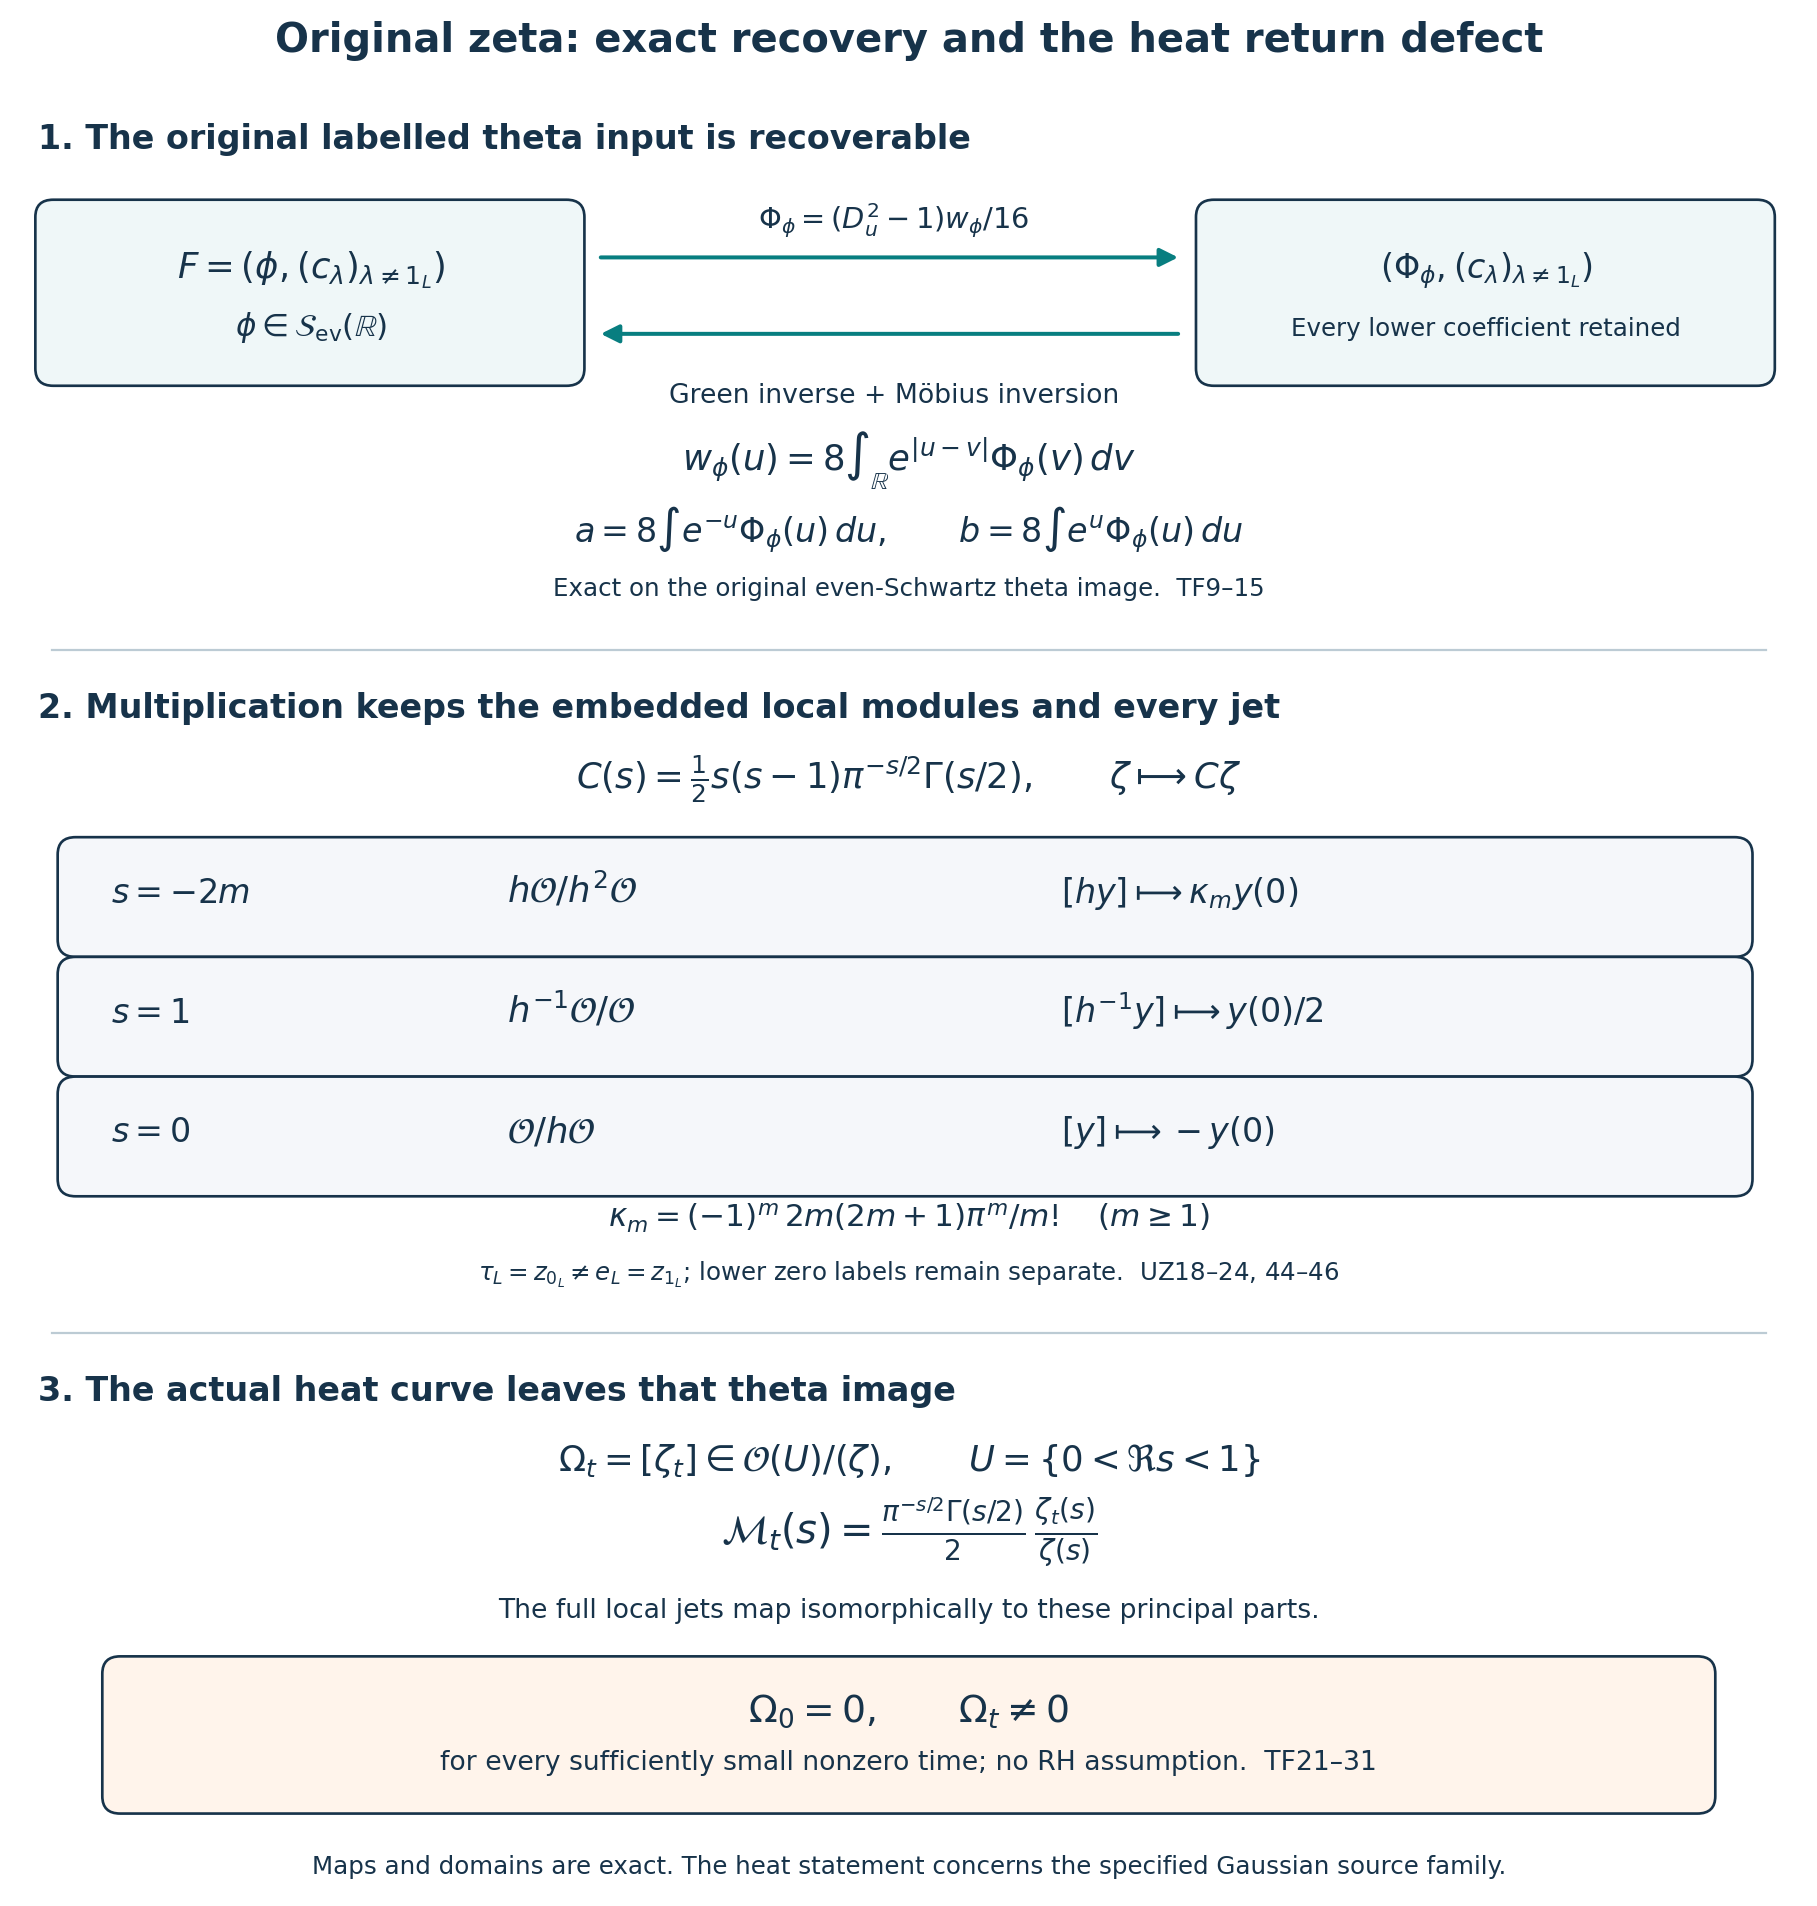
\includegraphics[keepaspectratio,alt={The exact original-zeta return. TF9--15 proves the filter and its inverse on the original even-Schwartz theta image, recovering both endpoints and every lower point-function coefficient. UZ18--24 and UZ44--46 prove the three embedded local fibre maps and retain all higher jets; h is the local coordinate s minus the point in each row. TF21--31 proves that the original Gaussian heat curve develops a nonzero return defect, and identifies its entire local jet tuple with the principal parts of the displayed meromorphic Mellin candidate. Its return obstruction is nonzero for every sufficiently small nonzero time. No zero location or RH assumption is used. Original heat convention: Rodgers--Tao, arXiv:1801.05914v5, equations hoz, phidef and htdef; every factor is retained in TF17--20.}]{faithful_theta_return.png}}
\caption{The exact original-zeta return. TF9--15 proves the filter and
its inverse on the original even-Schwartz theta image, recovering both
endpoints and every lower point-function coefficient. UZ18--24 and
UZ44--46 prove the three embedded local fibre maps and retain all higher
jets; h is the local coordinate s minus the point in each row. TF21--31
proves that the original Gaussian heat curve develops a nonzero return
defect, and identifies its entire local jet tuple with the principal
parts of the displayed meromorphic Mellin candidate. Its return
obstruction is nonzero for every sufficiently small nonzero time. No
zero location or RH assumption is used. Original heat convention:
Rodgers--Tao, arXiv:1801.05914v5, equations hoz, phidef and htdef; every
factor is retained in TF17--20.}
\end{figure}

\subsection{Original-zeta Gaussian and affine receiving
maps}\label{original-zeta-gaussian-and-affine-receiving-maps-3}

The complete extension OZG1--55 proves that Gaussian convolution of the
test at every positive time makes the original trivial-zero scalar sum
diverge for every real translation. Its admissible replacement retains
each cutoff trace and the Gamma boundary with the identical finite sum
U\_N; OZG20--27 gives both maps and the inverse. The full coefficient
tower, its raw non-Hermitian correction and exact compensated negative
index are OZG28--39. No compact-support prime window is assumed after
smoothing; all prime powers and Gamma terms, with explicit error bounds,
are OZG40--52. This extension acts on the tests while fixing the
original zeta zeros.

The different affine change of the actual original heat family is
OZR1--36. Its multiplier is exp(chi) C(phi)/C, with the full inverse,
exceptional units and local jets. The original generator contains every
q derivative term. The signed divisor comparison is OZR19--24; its
Cauchy logarithmic kernel has an additional growth contribution 2a.
OZR33 proves the exact full negative index after that contribution is
retained. The full support carrier and every lower coordinate are
OZG53--55 and OZR34--36. These are the receiving maps for these
specified extensions; the original preceding test, time and domains
remain those stated in its proof.

\clearpage

\section{Faithful completion, local fibres and the uncompleted zeta heat
equation}\label{faithful-completion-local-fibres-and-the-uncompleted-zeta-heat-equation}

This derivation retains the original meromorphic zeta function, the
complete completion factor, its factorization, every local fibre and
every support label. The completed function is a coordinate in an
explicitly isomorphic invertible sheaf. Ordinary evaluation after
forgetting that sheaf is a different map, computed below. The heat
family is the original Rodgers--Tao family in its original coordinates.
This derivation neither assumes an absolute-base origin for that author
construction nor asserts Riemann-hypothesis positivity.

\subsection{1. Sources, conventions and the original
family}\label{sources-conventions-and-the-original-family}

The original author source is Brad Rodgers and Terence Tao, \emph{The de
Bruijn--Newman constant is non-negative}, arXiv:1801.05914v5, equations
hoz, sas, phidef, htdef and the heat-equation sentence following htdef;
\href{https://arxiv.org/src/1801.05914v5}{author TeX}. Its canonical
local ID is PUBUNIT-8AD81C89CA3B6B4D23E6BC27; the author file
\texttt{sources/\allowbreak{}rodgers\_\allowbreak{}tao\_\allowbreak{}1801.\allowbreak{}05914v5/\allowbreak{}fmp-\allowbreak{}template.\allowbreak{}tex} has SHA256
\texttt{25b015c0\allowbreak{}fb151f16\allowbreak{}13247d82\allowbreak{}cf53a656\allowbreak{}1a320d4d\allowbreak{}ab2bb4f8\allowbreak{}09482e7c\allowbreak{}477a5817}.
The introductory definitions and their surrounding statements were read,
not inferred from a search hit.

The programme receivers used here are
\href{HEAT_CAUCHY_ARITHMETIC_DERIVATION.md}{HA1--16, HA20},
\href{ACTUAL_HEAT_ZERO_DISTRIBUTION_VARIATION.md}{AG1--9, AG18--24},
\href{REAL_TIME_HEAT_TRACE_DERIVATION.md}{RT1--18}, and
\href{SUPPORTED_ZERO_PRIME_WEIL_DERIVATION.md}{SZW1--19, SZW24--38}. HA
supplies the unchanged completion logarithmic derivative and full
arithmetic terms; AG supplies the rational trace theorem and specified
contour variation; RT supplies the actual right-time compact-test
derivative. SZW supplies the supported-zero theta comparison and label
spaces. This note proves the additional completion/sheaf comparisons and
local calculations in full.

Write \[
\begin{aligned}
B(s)&=\pi^{-s/2}\Gamma(s/2),&
p(s)&=\tfrac12s(s-1),&
C(s)&=p(s)B(s),\\
\xi(s)&=C(s)\zeta(s),&
\Lambda(s)&=B(s)\zeta(s),&
\xi(s)&=p(s)\Lambda(s).
\end{aligned}\tag{UZ1}
\] The symbol \(p(s)\) in this factorization is a polynomial, not a
finite prime. The factor \(1/2\), the two endpoint factors and the whole
Gamma factor remain in every map.

The original heat family and its transported coordinate are \[
\begin{aligned}
\Phi(u)&=\sum_{n\ge1}(2\pi^2n^4e^{9u}-3\pi n^2e^{5u})e^{-\pi n^2e^{4u}},\\
H_t(z)&=\int_0^\infty e^{tu^2}\Phi(u)\cos(zu)\,du,\\
\xi_t(s)&=8H_t(-2i(s-\tfrac12)),\qquad
g_t(s)=2\xi_t(s)=16H_t(-2i(s-\tfrac12)),\\
\zeta_t(s)&=C(s)^{-1}\xi_t(s),\qquad
\Lambda_t(s)=B(s)\zeta_t(s)=\frac{2\xi_t(s)}{s(s-1)}.
\end{aligned}\tag{UZ2}
\] Thus \(\xi_0=\xi,\ \zeta_0=\zeta,\ g_0=2\xi\), and
\(\Lambda_t=g_t/(s(s-1))\), exactly as in HA20.

For \(u\ge0\), splitting the exponential in the \(n\)-sum gives \[
|\Phi(u)|\le K e^{9u-ce^{4u}}\quad(c>0).
\tag{UZ3}
\] Indeed one half of \(\pi n^2e^{4u}\) bounds a positive multiple of
\(e^{4u}\), while the other half makes \(\sum n^4e^{-\pi n^2/2}\)
summable. On compact sets of complex \(s,t\), derivatives of the
integrand add powers of \(u\), still bounded by an integrable function
\(K'\exp(Tu^2+(2R+10)u-ce^{4u})\). Consequently \(\xi_t(s)\) is jointly
entire in \((t,s)\), and direct differentiation, retaining
\((-2i)^2=-4\), gives \[
\partial_t\xi_t=\tfrac14\partial_s^2\xi_t,\qquad
\xi_t(1-s)=\xi_t(s).
\tag{UZ4}
\] For no complex \(t\) is \(\xi_t\) the zero function. To see this,
extend \(e^{tu^2}\Phi(u)\) evenly from the positive half-line. Its
extension is in \(L^1(\mathbb R)\) by (UZ3), is nonzero, and its Fourier
transform is \(2H_t\) on the real axis. If that transform vanished
identically, convolution with each Gaussian approximate identity would
vanish by Fourier inversion for the Gaussian and Fubini's theorem.
Approximation in \(L^1\) would make the original function zero, a
contradiction. Thus all divisors used below are defined, including at
complex times.

For real \(t,s\), every summand of \(\Phi(u)\) is positive because
\(2\pi n^2e^{4u}-3>0\), and the cosine in (UZ2) becomes
\(\cosh(2(s-\tfrac12)u)>0\). Hence \[
\xi_t(s)>0\quad(t,s\in\mathbb R).
\tag{UZ5}
\] This does not assert positivity of a Weil quadratic form.

\subsection{2. Gamma factors and their exact local
units}\label{gamma-factors-and-their-exact-local-units}

Here are the Gamma facts and their sufficient derivation. Euler's limit
and its reciprocal product are \[
\Gamma(z)=\lim_{N\to\infty}\frac{N!\,N^z}{z(z+1)\cdots(z+N)},\qquad
\frac1{\Gamma(z)}
=z e^{\gamma z}\prod_{n\ge1}(1+z/n)e^{-z/n}.
\tag{UZ6}
\] The first follows for \(\Re z>0\) from \[
\int_0^1x^{z-1}(1-x)^Ndx
=\frac{N!}{z(z+1)\cdots(z+N)}
\] by repeated integration by parts, substitution \(y=Nx\), and
dominated convergence using \((1-y/N)^N\le e^{-y}\). For the reciprocal
product use \(\sum_{n\le N}1/n-\log N\to\gamma\). The factors after
their linear terms have uniformly summable logarithms on every compact
set avoiding \(-1,-2,\ldots\). This proves local uniform convergence and
nonvanishing there. Thus the reciprocal is entire, its zeros are simple
and occur exactly at \(0,-1,-2,\ldots\), and \(\Gamma\) has no zeros.
The integral also gives \(\Gamma(z+1)=z\Gamma(z)\) and \(\Gamma(1)=1\).

Taking logarithms near zero gives the convergent identity \[
\log\Gamma(1+z)
=-\gamma z+\sum_{k\ge2}\frac{(-1)^k\zeta(k)}k z^k,\qquad |z|<1.
\tag{UZ7}
\] To verify it, expand \(\log(1+z/n)\) in (UZ6), interchange the
absolutely convergent double series for \(|z|<1\), and retain the linear
term separately. In this formula \(\zeta(k)=\sum_{n\ge1}n^{-k}\), with
\(k\ge2\), needs no analytic continuation.

Let \(u=s-s_*\). Write \(C(s_*+u)=u^d c_{s_*}(u)\), where \(c_{s_*}\) is
a holomorphic unit. At zero there is no residual zero or pole: \[
d=0,\qquad
c_0(u)=(u-1)\pi^{-u/2}\Gamma(1+u/2),\qquad c_0(0)=-1,
\tag{UZ8}
\] and the full convergent unit expansion is specified by \[
\log\frac{c_0(u)}{-1}
=\log(1-u)-\frac{\gamma+\log\pi}{2}u
+\sum_{k\ge2}\frac{(-1)^k\zeta(k)}{k2^k}u^k,\qquad |u|<1.
\tag{UZ9}
\] The branch has value zero at \(u=0\). In particular
\(C'(0)=1+(\gamma+\log\pi)/2\).

At \(s=1\), \[
d=1,\qquad
c_1(u)=\tfrac12(1+u)\pi^{-(1+u)/2}\Gamma((1+u)/2),\qquad
c_1(0)=\tfrac12,
\tag{UZ10}
\] and \[
\begin{aligned}
\log\frac{c_1(u)}{1/2}
={}&\log(1+u)
-\left(\frac{\gamma+\log\pi}{2}+\log2\right)u\\
&+\sum_{k\ge2}\frac{(-1)^k(1-2^{-k})\zeta(k)}k u^k,
\qquad |u|<1.
\end{aligned}\tag{UZ11}
\] For the value \(\Gamma(1/2)=\sqrt\pi\), square the positive Gaussian
integral and change to polar coordinates. For the logarithmic series,
differentiating (UZ6) gives
\(\psi(z)=-\gamma+\sum_{n\ge0}(1/(n+1)-1/(n+z))\). At \(z=1/2\) the
partial sums reduce to \(2(H_{N+1}-H_{2N+2})\to-2\log2\), so
\(\psi(1/2)=-\gamma-2\log2\). For \(k\ge2\), termwise differentiation
gives the Taylor coefficient \((-1)^k\sum_{n\ge0}(n+1/2)^{-k}/k\); after
the substitution \(z=1/2+u/2\) it is \((-1)^k(1-2^{-k})\zeta(k)/k\).
This proves (UZ11), including its linear coefficient.

At \(s=-2m,\ m\ge1\), put \[
\kappa_m=(-1)^m\frac{2m(2m+1)\pi^m}{m!}.
\tag{UZ12}
\] The complete local expression, retaining its original factors, is \[
\begin{aligned}
d&=-1,\qquad C(-2m+u)=u^{-1}c_{-2m}(u),\\
c_{-2m}(u)
&=\kappa_m
\left(1-\frac{u}{2m}\right)
\left(1-\frac{u}{2m+1}\right)
\pi^{-u/2}\Gamma(1+u/2)
\prod_{j=1}^{m}\left(1-\frac{u}{2j}\right)^{-1}.
\end{aligned}\tag{UZ13}
\] Indeed Gamma recurrence gives \[
\Gamma(-m+u/2)
=\frac{2(-1)^m}{m!\,u}\Gamma(1+u/2)
\prod_{j=1}^m(1-u/(2j))^{-1}.
\] Multiplication by \(\tfrac12(-2m+u)(-2m-1+u)\pi^{m-u/2}\) proves
(UZ13). In particular \(c_{-2m}(0)=\kappa_m\), with its sign retained.

For \(H_m^{(k)}=\sum_{j=1}^m j^{-k}\) and \(H_m=H_m^{(1)}\), the full
convergent logarithmic series on \(|u|<1\) is \[
\begin{aligned}
\log\frac{c_{-2m}(u)}{\kappa_m}
={}&\left[-\frac1{2m}-\frac1{2m+1}
-\frac{\gamma+\log\pi}{2}+\frac{H_m}{2}\right]u\\
&+\sum_{k\ge2}\frac1k
\left[
\frac{(-1)^k\zeta(k)+H_m^{(k)}}{2^k}
-\frac1{(2m)^k}-\frac1{(2m+1)^k}
\right]u^k .
\end{aligned}\tag{UZ14}
\] It follows by expanding every factor in (UZ13); convergence is
absolute on compact subdiscs. Equations (UZ9), (UZ11), (UZ14), followed
by exponentiation, specify all unit coefficients, not only leading
values. At every other finite point \(s_*\), \(d=0\) and
\(c_{s_*}(u)=C(s_*+u)\) is already a holomorphic unit.

The full factor divisors are therefore \[
\operatorname{div}B=-[0]-\sum_{m\ge1}[-2m],\quad
\operatorname{div}p=[0]+[1],\quad
D:=\operatorname{div}C=[1]-\sum_{m\ge1}[-2m].
\tag{UZ15}
\] Each sum is locally finite. The \([0]\) terms cancel as divisors; the
factors \(B,p\), their residues and their full units remain part of
(UZ1). In particular ``zero divisor coefficient at 0'' does not say that
these factors or the supported-zero endpoint data were absent.

\subsection{3. The invertible sheaf and all local
jets}\label{the-invertible-sheaf-and-all-local-jets}

Let \(X=\mathbb C\), \(\mathcal O=\mathcal O_X\) be the holomorphic
sheaf and \(\mathcal M\) the meromorphic sheaf. Define the embedded
fractional ideal sheaf \[
\mathcal L=\mathcal O(D)
:=\{f\in\mathcal M:\operatorname{div}f+D\ge0\}
=C^{-1}\mathcal O\subset\mathcal M.
\tag{UZ16}
\] The inequality is local at every finite point. Multiplication is an
everywhere invertible sheaf morphism \[
M_C:\mathcal L\xrightarrow{\;\sim\;}\mathcal O,\quad f\mapsto Cf,
\qquad M_C^{-1}(F)=C^{-1}F .
\tag{UZ17}
\] Proof: both compositions are the identity in \(\mathcal M\); (UZ16)
is precisely the condition that \(Cf\) be holomorphic. At \(s_*\), if
\(C=u^dc(u)\), then \(\mathcal L_{s_*}=u^{-d}\mathcal O_{s_*}\), because
\(c\) is a unit. Thus the morphism is an isomorphism at every stalk, not
only off the completion divisor. Multiplication by \(C\) is also an
automorphism of the \(\mathcal O\)-module \(\mathcal M\), but retaining
\((\mathcal O,\mathcal L,\mathcal O\hookrightarrow\mathcal M,\mathcal L\hookrightarrow\mathcal M,C)\)
additionally retains the original orders of vanishing and poles.

Write \(f=u^{-d}y(u)\), \(Cf=x(u)=c(u)y(u)\), with
\(x=\sum x_j u^j,\ y=\sum y_j u^j,\ c=\sum c_j u^j\). For every
\(N\ge0\), (UZ17) induces the fibre-and-jet isomorphism \[
\begin{aligned}
\mathcal L_{s_*}/u^{N+1}\mathcal L_{s_*}
&\xrightarrow{\;\sim\;}
\mathcal O_{s_*}/u^{N+1}\mathcal O_{s_*},\\
x_j&=\sum_{i=0}^{j}c_i y_{j-i},\qquad
y_j=c_0^{-1}\left(x_j-\sum_{i=1}^{j}c_i y_{j-i}\right)
\quad(0\le j\le N).
\end{aligned}\tag{UZ18}
\] The diagonal coefficient is \(c_0\ne0\), so the displayed recurrence
proves bijectivity for every finite jet order and for the inverse-limit
formal completion. Analytic sections are related by the convergent
multiplication and division in (UZ17). This keeps all derivatives and
Laurent coefficients with their exact index shift.

At the three types of special point, the fibre maps are as follows: \[
\begin{array}{c|c|c|c}
s_* & \mathcal L_{s_*} & \mathcal L_{s_*}/u\mathcal L_{s_*}
& M_C\text{ on that fibre}\\ \hline
-2m & u\mathcal O_{s_*} & u\mathcal O_{s_*}/u^2\mathcal O_{s_*}
& [u y]\mapsto \kappa_m y(0)\\
1 & u^{-1}\mathcal O_1 & u^{-1}\mathcal O_1/\mathcal O_1
& [u^{-1}y]\mapsto \tfrac12 y(0)\\
0 & \mathcal O_0 & \mathcal O_0/u\mathcal O_0
& [y]\mapsto -y(0).
\end{array}\tag{UZ19}
\] At \(-2m\), the inclusion \(u\mathcal O\hookrightarrow\mathcal O\)
induces the zero map into \(\mathcal O/u\mathcal O\), since \(uy\)
evaluates to zero. Its source fibre \(u\mathcal O/u^2\mathcal O\) is one
dimensional and need not be zero. The completion map instead multiplies
that fibre by \(\kappa_m\), an isomorphism. At 1 there is no ordinary
holomorphic evaluation of \(u^{-1}y\); the correct fibre records its
residue \(y(0)\). Evaluating \(C(1)=0\) and treating \(u^{-1}y\) as a
scalar value would not be a defined map. These conclusions compute the
maps responsible for the apparent losses.

There is also the faithful intermediate factorization \[
\begin{aligned}
\mathcal L_\Lambda&=p^{-1}\mathcal O
=\mathcal O([0]+[1])\subset\mathcal M,\\
\mathcal L \xrightarrow{\,M_B\,}\mathcal L_\Lambda
&\xrightarrow{\,M_p\,}\mathcal O,\qquad
M_pM_B=M_C,
\end{aligned}\tag{UZ20}
\] with both arrows isomorphisms. In fact \(pf_\Lambda\) is holomorphic
iff \(f_\Lambda\in\mathcal L_\Lambda\), and \(p(Bf)=Cf\), which proves
the first arrow and its inverse. This preserves the Gamma pole at zero
before the \(s\)-factor acts.

For completeness, the classical values and leading coefficients follow
without assuming trivial-zero simplicity. On \(\Re s>1\), integrating
the counting function \(\lfloor x\rfloor\) gives \[
\zeta(s)=s\int_1^\infty \lfloor x\rfloor x^{-s-1}dx
=\frac{s}{s-1}-s\int_1^\infty\{x\}x^{-s-1}dx.
\tag{UZ21}
\] The last integral is holomorphic on \(\Re s>0\), by boundedness of
\(\{x\}\) and differentiation on compact subsets. Thus the residue of
\(\zeta\) at 1 is 1. Equations (UZ10) and \(\xi(1-s)=\xi(s)\) imply \[
\xi(1)=\xi(0)=\tfrac12,\quad
\zeta(0)=-\tfrac12,\quad
\operatorname{Res}_{s=0}\Lambda=-1,\quad
\operatorname{Res}_{s=1}\Lambda=1.
\tag{UZ22}
\] At \(-2m\), reflection gives \[
\begin{aligned}
\xi(-2m)&=\xi(2m+1)
=\frac{m(2m+1)(2m)!}{4^m m!\pi^m}\zeta(2m+1)>0,\\
\zeta'(-2m)&=\frac{\xi(-2m)}{\kappa_m}
=(-1)^m\frac{(2m)!}{2(2\pi)^{2m}}\zeta(2m+1).
\end{aligned}\tag{UZ23}
\] To obtain the first expression use
\(\Gamma(m+1/2)=(2m)!\sqrt\pi/(4^m m!)\), proved from Gamma recurrence
and the Gaussian integral. The second follows by the first-fibre map in
(UZ19). It is nonzero, so these are simple trivial zeros. No zero or
coefficient has been identified with the unsupported element.

For every real time, (UZ5) and the same local maps give the exact
persistent geometry \[
\begin{aligned}
\operatorname{Res}_{s=1}\zeta_t&=2\xi_t(1)>0,&
\zeta_t(0)&=-\xi_t(0)<0,\\
\zeta_t'(-2m)&=\xi_t(-2m)/\kappa_m,&
\operatorname{sgn}\zeta_t'(-2m)&=(-1)^m,\\
\operatorname{Res}_{s=0}\Lambda_t&=-2\xi_t(0),&
\operatorname{Res}_{s=1}\Lambda_t&=2\xi_t(1).
\end{aligned}\tag{UZ24}
\] In particular the pole and trivial-zero orders remain exactly simple
for real \(t\). For complex \(t\) the sheaf maps and divisor identity
remain valid, but a zero of \(\xi_t\) at one of these points can change
the total order; no fixed-order assertion is made for complex time.

\subsection{4. The complete transported heat
operator}\label{the-complete-transported-heat-operator}

Put \(q=C'/C\). As a meromorphic function its exact expression is \[
\begin{aligned}
q(s)&=\frac1s+\frac1{s-1}-\frac{\log\pi}{2}
+\frac12\psi(s/2),\\
q'(s)&=-\frac1{s^2}-\frac1{(s-1)^2}
+\frac14\psi^{(1)}(s/2),\\
\frac{C''}{C}(s)
&=\left(\frac1s+\frac1{s-1}-\frac{\log\pi}{2}
+\frac12\psi(s/2)\right)^2
-\frac1{s^2}-\frac1{(s-1)^2}
+\frac14\psi^{(1)}(s/2).
\end{aligned}\tag{UZ25}
\] Here \(\psi=\Gamma'/\Gamma\). These formulas are valid
meromorphically, with the removable singularity at 0 assigned the unit
value from (UZ9); for example \(q(0)=-1-(\gamma+\log\pi)/2\). At 1 and
\(-2m\) the residues of \(q\) are respectively \(+1\) and \(-1\),
precisely the divisor coefficients in (UZ15).

Since \(C\) does not depend on \(t\), (UZ4) proves \[
\boxed{\quad
\partial_t\zeta_t
=\tfrac14\left[
\partial_s^2\zeta_t
+2q(s)\partial_s\zeta_t
+\bigl(q'(s)+q(s)^2\bigr)\zeta_t
\right]
=\tfrac14 C^{-1}\partial_s^2(C\zeta_t).
\quad}\tag{UZ26}
\] It follows by expanding \(\partial_s^2(C\zeta_t)\), without deleting
any factor of \(C\). In particular the uncompleted function does not
satisfy the coefficient-free heat equation in this coordinate. For real
time, \(\zeta_t''\) has a pole of order three at 1 with nonzero leading
coefficient, by (UZ24), whereas \(\partial_t\zeta_t\) has at most a
simple pole there because \(C^{-1}\) is fixed and \(\partial_t\xi_t\) is
entire.

The operator is defined across all special points as the connection \[
\nabla_C:\mathcal L\to\mathcal L,\qquad
\nabla_C f=C^{-1}\partial_s(Cf),\qquad
\partial_t\zeta_t=\tfrac14\nabla_C^2\zeta_t .
\tag{UZ27}
\] It maps \(\mathcal L\) to itself because derivatives of a holomorphic
function are holomorphic. It satisfies \(\nabla_C(af)=a'f+a\nabla_C f\)
for \(a\in\mathcal O\). Thus its meromorphic coefficient presentation
does not make its action on the retained lattice undefined.

More explicitly, at every \(s_*\) write \(\zeta_t=u^{-d}y_t(u)\),
\(C=u^dc(u)\). The full local heat equation is \[
\partial_t y_t
=\tfrac14\left[y_t''+2\frac{c'}c y_t'
+\frac{c''}c y_t\right].
\tag{UZ28}
\] Indeed \(\xi_t=cy_t\), and the time-independent factor \(u^{-d}\)
cancels only as a change of local frame in (UZ26). Equivalently,
differentiating \(u^{-d}y\) and using \(q=d/u+c'/c\) cancels each
displayed \(1/u\) term in the connection. The complete unit \(c\), given
in (UZ8), (UZ10), (UZ13), remains. Its coefficients are holomorphic on
the local disc.

All jets evolve through these same maps. For
\(x_t=\xi_t=\sum x_j(t)u^j\), \[
4\dot x_j=(j+2)(j+1)x_{j+2}.
\tag{UZ29}
\] The dot denotes a complex analytic local time derivative, justified
by joint entire dependence in (UZ3). If \(a(u)=c'/c=\sum a_i u^i\),
\(b(u)=c''/c=\sum b_i u^i\), and \(y_t=\sum y_j(t)u^j\), (UZ28) gives \[
4\dot y_j=(j+2)(j+1)y_{j+2}
+2\sum_{i=0}^j a_i(j-i+1)y_{j-i+1}
+\sum_{i=0}^j b_i y_{j-i}.
\tag{UZ30}
\] The recurrence (UZ18) intertwines (UZ29) and (UZ30). Finite jets are
not falsely claimed to form an autonomous heat system: their derivatives
use the two additional jet orders displayed in these equations.

On \(\Re s>1\), at \(t=0\), the logarithmic derivative of \(\xi\) is \[
L_0=q+\zeta'/\zeta
=q-\sum_{n\ge2}\Lambda(n)n^{-s}.
\tag{UZ31}
\] This is exactly HA10, with its original endpoint and Gamma terms.
Differentiating the logarithmic derivative in time gives \[
\partial_t(\zeta_t'/\zeta_t)
=\partial_t(\xi_t'/\xi_t)
=\tfrac14\partial_s(\xi_t''/\xi_t).
\tag{UZ32}
\] The first equality holds because \(q\) is independent of \(t\). Hence
the full causal distribution in CH and its archimedean--prime mixed
terms are unchanged by the faithful uncompleted coordinate. In
particular replacing \(q\) by zero would change the actual heat
variation and would discard the mixed terms, rather than implement
(UZ17).

Reflection also transports exactly. Let \(R(F)(s)=F(1-s)\). Then \[
J_C:=M_C^{-1}RM_C,\qquad
(J_C f)(s)=\frac{C(1-s)}{C(s)}f(1-s),\qquad
J_C^2=\mathrm{id}_{\mathcal L}.
\tag{UZ33}
\] These are operators on global sections; on local sections the
reflected operator sends sections over \(U\) to sections over \(1-U\),
so its sheaf map covers the reflection of the base and is not
\(\mathcal O\)-linear over the identity map. Proof: \(Cf\) is
holomorphic, so its reflection is holomorphic on the reflected domain,
proving the stated codomain; composition cancels the two meromorphic
ratios and gives the identity. Also \[
\nabla_C J_C=-J_C\nabla_C,\qquad
\nabla_C^2J_C=J_C\nabla_C^2,\qquad
J_C\zeta_t=\zeta_t.
\tag{UZ34}
\] The first relation is the chain rule after conjugating by \(C\); the
others follow by a second application and (UZ4). No unweighted
reflection of the uncompleted meromorphic coordinate is substituted for
this operator.

\subsection{5. Divisors, finite contours and global
traces}\label{divisors-finite-contours-and-global-traces}

The exact meromorphic divisor relation for every time is \[
\operatorname{div}\zeta_t=\operatorname{div}\xi_t-D
=\operatorname{div}\xi_t+\sum_{m\ge1}[-2m]-[1].
\tag{UZ35}
\] It is an identity of locally finite signed divisors. It follows at
each stalk from
\(\operatorname{ord}(C\zeta_t)=\operatorname{ord}C+\operatorname{ord}\zeta_t\).
If \(\xi_t\) vanishes at a special point, the orders add there; the
formula still holds.

Let \(\Omega\) be bounded with a piecewise smooth boundary avoiding the
zeros and poles of the functions involved, and let \(A\) be holomorphic
near \(\overline\Omega\). The exact finite-contour map is \[
\begin{aligned}
\frac1{2\pi i}\int_{\partial\Omega}
 A(s)\frac{\zeta_t'(s)}{\zeta_t(s)}\,ds
&=\frac1{2\pi i}\int_{\partial\Omega}
 A(s)\frac{\xi_t'(s)}{\xi_t(s)}\,ds
-\frac1{2\pi i}\int_{\partial\Omega}A(s)q(s)\,ds\\
&=\sum_{\rho\in\Omega}\operatorname{ord}_\rho(\xi_t)A(\rho)
+\sum_{-2m\in\Omega}A(-2m)-1_{\{1\in\Omega\}}A(1).
\end{aligned}\tag{UZ36}
\] Each sum is finite and includes multiplicity. This is the residue
theorem applied to \(\zeta_t'/\zeta_t=\xi_t'/\xi_t-q\). It applies
without a summability assumption on an infinite trivial-zero sequence.
If a test has a pole inside \(\Omega\), its additional residues must
also be retained; (UZ36) is stated with the holomorphic-test hypothesis
to avoid suppressing them.

For a fixed such contour nonvanishing persists at sufficiently small
complex time, so differentiating (UZ36) gives equality of its two heat
variations, since the \(q\) integral is fixed. Thus the equality holds
before an infinite contour limit, including at every trivial-zero and
endpoint local geometry.

Now let \(A\) be rational, \(A(s)=O(s^{-2})\) at infinity, with poles
avoiding \(1,-2,-4,\ldots\) and the zeros of \(\xi_{t_*}\) at a real
time \(t_*\). There is a complex time neighbourhood of \(t_*\) in which
\[
\boxed{\quad
Z_{\zeta_t}^{\mathrm{div}}(A)
=Z_{\xi_t}(A)+\sum_{m\ge1}A(-2m)-A(1).
\quad}\tag{UZ37}
\] The left side is the sum of the signed divisor orders against \(A\);
the right side retains all its three parts. Both sums converge
absolutely. To prove it, (UZ3) yields the uniform growth
\(\log\max_{|s|\le R}|\xi_t(s)|\le K(R+1)\log(R+2)\): absorb \(Tu^2\)
into half of \(ce^{4u}\), then substitute \(x=e^{4u}\) in the remaining
integral and bound the resulting Gamma integral. Since
\(\xi_{t_*}(0)>0\), it remains nonzero in a small complex time disc.
Jensen's formula then gives \(N_t(R)=O(R\log(R+2))\), uniformly there.
Dyadic summation implies
\(\sum_{|\rho|>R}m_\rho|\rho|^{-2}=O(\log(R+2)/R)\). Also
\(A(-2m)=O(m^{-2})\). These bounds prove absolute convergence, and
summing (UZ35) proves (UZ37).

For clarity, the derivative in (UZ37) is a genuine derivative of the
infinite rational trace. The genus-one logarithmic derivative is \[
\frac{\xi_t'}{\xi_t}(s)
=b_t+\sum_\rho m_\rho\left(\frac1{s-\rho}+\frac1\rho\right).
\] It converges normally on compact sets avoiding the zeros by the
preceding square-summability estimate. Summing residues at the finite
pole set \(\mathcal P(A)\) gives \[
Z_{\xi_t}(A)
=-\sum_{a\in\mathcal P(A)}
\operatorname{Res}_{s=a}
\left(A(s)\frac{\xi_t'(s)}{\xi_t(s)}\right).
\tag{UZ38}
\] Indeed \(\sum_a\operatorname{Res}_a A=0\), so \(b_t\) and every
constant \(1/\rho\) correction contribute zero, and the rational
function \(A(s)/(s-\rho)\) has pole-set residues summing to
\(-A(\rho)\). Normal convergence permits termwise residues. The right
side is holomorphic in time while its finite pole values avoid zeros.
Hence \[
\partial_t Z_{\zeta_t}^{\mathrm{div}}(A)
=\partial_t Z_{\xi_t}(A)
=-\frac14\sum_{a\in\mathcal P(A)}
\operatorname{Res}_{s=a}
\left(A(s)\partial_s\frac{\xi_t''(s)}{\xi_t(s)}\right).
\tag{UZ39}
\] This proves equality of the actual derivatives, not an unsupported
interchange with individually moving zero sums.

For entire compact-test Mellin transforms this rational summability
conclusion must not be transplanted. With the original convention \[
A(s)=M_h(s)=\int_{\mathbb R}h(v)e^{-(s-1/2)v}dv,
\tag{UZ40}
\] choose a nonzero nonnegative \(h\in C_c^\infty((a,b))\) with
\(0<a<b\). Then \[
M_h(-2m)\ge e^{(2m+1/2)a}\int h(v)dv,
\tag{UZ41}
\] so \(\sum_mM_h(-2m)\) diverges. Even endpoint filtering does not
repair this: for \(T=\partial_v^2-1/4\), two integrations by parts give
\[
M_{Th}(s)=s(s-1)M_h(s),
\] so its values at \(-2m\) have the additional positive factor
\(2m(2m+1)\) and still diverge. The values at 0 and 1 vanish, which is a
different exact statement.

There is nevertheless a faithful finite-contour and regularized map.
Retain at every \(\Omega\) the pair \[
\left(
Z_{\zeta_t,\Omega}^{\mathrm{div}}(A),\
D_\Omega(A):=\frac1{2\pi i}\int_{\partial\Omega}Aq\,ds
\right),\qquad
Z_{\zeta_t,\Omega}^{\mathrm{div}}(A)+D_\Omega(A)=Z_{\xi_t,\Omega}(A).
\tag{UZ42}
\] Retain also the actual divisors \(\operatorname{div}\zeta_t|_\Omega\)
and \(D|_\Omega\), rather than only their value under a single test.
Restriction to nested domains then records each added divisor point and
its order; this is the faithful locally finite divisor data. A single
weighted value can vanish at a nonempty divisor and is not an injective
encoding. For real \(t\ge0\), RT1--18 provides the critical strip and
complete compact-test trace. Exhausting the plane by bounded domains
with boundaries avoiding the divisors then gives the specified relative
trace \[
Z_{\zeta_t;C}^{\mathrm{rel}}(M_h)
:=\lim_{\Omega\uparrow\mathbb C}
\left(Z_{\zeta_t,\Omega}^{\mathrm{div}}(M_h)+D_\Omega(M_h)\right)
=Z_{\xi_t}(M_h).
\tag{UZ43}
\] The limit exists because the terms inside parentheses equal the
finite completed trace exactly and the completed zero sum converges
absolutely: compact smooth Mellin tests decrease faster than every power
on the closed critical strip, and the zero count above applies. The two
separate terms in parentheses need not converge. The definition is
therefore a relative trace with its fixed divisor correction explicitly
retained, not a convergent unsigned trivial-zero sum.

At time zero, on the separated-height contours of AG22, or any
enlargement adding the fixed real divisor points and excluding zeros on
its boundary, the \(D_\Omega\) contribution has derivative zero. The
limit of finite-contour derivatives is consequently the original AG20
variation. RT16 further proves that on the real \(t\ge0\) family this
variation is the actual right derivative of (UZ43) for compact smooth
\(h\). These are the specified contour map and the independently proved
actual-time upgrade; no unproved complex-time entire-test convergence is
inserted.

\subsection{6. The supported carrier and retained endpoint
representations}\label{the-supported-carrier-and-retained-endpoint-representations}

Let \(L\) be the original finite bounded distributive support lattice.
Use exactly the SZW10 carrier, extended to meromorphic amplitudes: \[
G_L(\mathcal M)
=\{(f,1_L):f\in\mathcal M\}
\cup\{z_\lambda=(0,\lambda):\lambda\ne1_L\},\qquad
\tau=z_{0_L},\quad e=z_{1_L}.
\] No nonzero amplitude is assigned a nontop label. The original
addition uses amplitude addition and support join; multiplication uses
amplitude multiplication and support meet. These operations preserve the
displayed set: if an amplitude sum or product is nonzero, each factor
that could force a nontop support has been excluded by that nonzero
amplitude. More explicitly, a nonzero sum has at least one top-labelled
summand, and a nonzero product has both factors top-labelled. The
element \(\tau=z_{0_L}\) is the additive identity and is
multiplicatively absorbing. These operations respect restriction of
sections. In particular \(e\ne\tau\) for a nontrivial support lattice.
The multiplication map is \[
\widehat M_C(z_\lambda)=z_\lambda,\qquad
\widehat M_C(f,1_L)=(Cf,1_L),\qquad
\widehat M_C^{-1}(F,1_L)=(C^{-1}F,1_L).
\tag{UZ44}
\] It is an additive, label-preserving bijection between the carrier
over \(\mathcal L\) and the carrier over \(\mathcal O\); the two
prescriptions agree at \(e=(0,1_L)\). It is multiplication by
\((C,1_L)\) in the ambient meromorphic semiring, and its inverse is
multiplication by \((C^{-1},1_L)\). It fixes every \(z_\lambda\),
including the distinct elements \(e\) and \(\tau\).

For precision this is a module/scalar-multiplication isomorphism, not a
claim that multiplication by \(C\) is a ring homomorphism. Moreover
\(\mathcal O(D)\) is not generally closed under multiplication in its
embedding: its natural product is
\(\mathcal O(D)\otimes\mathcal O(D)\to\mathcal O(2D)\). The
corresponding exact multiplicative square uses \(M_{C^2}\) on
\(\mathcal O(2D)\), since \((Cf)(Cg)=C^2fg\). Thus product domains and
all labels are retained.

At a special point, first apply the stalk/fibre morphism (UZ18) on the
top amplitude, leaving each lower zero label unchanged. This gives, for
example, \[
([u y],1_L)\longmapsto(\kappa_m y(0),1_L)
\quad\text{at }-2m,\qquad
([u^{-1}y],1_L)\longmapsto(\tfrac12y(0),1_L)
\quad\text{at }1,\qquad z_\lambda\longmapsto z_\lambda.
\tag{UZ45}
\] If a top fibre coefficient is zero, its image is \(e=(0,1_L)\); it is
never \(\tau\). At \(-2m\), the ambient holomorphic evaluation instead
gives \(e\), regardless of the derivative coefficient. Equation (UZ19)
proves exactly why that different map loses the first nonzero
coefficient. The faithful sheaf map retains it, and the independent
lower labels remain fixed.

Finally SZW's full endpoint representation and every lower fixed
coordinate can be carried as direct, unchanged components: \[
M_C\oplus\mathrm{id}_{V_L}:
\mathcal L\oplus V_L\longrightarrow\mathcal O\oplus V_L,
\tag{UZ46}
\] where \(V_L\) is the original endpoint/lower-label vector space of
SZW13 and SZW33--38. This formula is read on the spaces of sections
together with the attached fixed representation; its inverse is
\(M_{C^{-1}}\oplus\mathrm{id}_{V_L}\). The arbitrary complex
\(c_\lambda\) are values of functions \textbf{on} the lower carrier
points, as in SZW11. They are not nonzero amplitudes \textbf{in} the
carrier at nontop labels. This distinction retains both the exact set in
SZW10 and all its independent function coordinates. Equations (UZ20),
(UZ22), (UZ24) additionally retain the meromorphic residues of
\(\Lambda_t\) at both endpoints. A fixed supported-zero trace, an
endpoint residue, a divisor order, a local section coefficient and an
unsupported element have the connecting maps above; none has been
replaced by another object merely because a scalar coefficient vanishes.

The classical author construction (UZ2) is presented over complex \(s\),
complex-valued functions and real heat time, with joint complex analytic
extension justified here. The programme's lift (UZ44) and its augmented
endpoint map (UZ46) are explicit additional constructions. Their
existence does not prove that the original author heat kernel was
defined over the absolute base. Completion is useful here because it
gives an entire heat coordinate and its reflection; uncompletion through
(UZ17), (UZ20), (UZ26), (UZ35) and (UZ42) preserves the full local and
supported data. The signs in (UZ23)--(UZ24) concern exact real local
coefficients, and do not establish positivity of the full reflected Weil
pairing.

\subsection{7. All reflected local orientations and the unchanged
nontrivial
divisor}\label{all-reflected-local-orientations-and-the-unchanged-nontrivial-divisor}

Write \(\mathcal R_C(s)=C(1-s)/C(s)\), retaining this quotient as the
definition. Substitution of (UZ1), with both polynomial factors retained
before the equality is taken, proves the meromorphic identity \[
\mathcal R_C(s)=
\frac{\frac12(1-s)(-s)\pi^{-(1-s)/2}\Gamma((1-s)/2)}
{\frac12s(s-1)\pi^{-s/2}\Gamma(s/2)}
=\pi^{s-1/2}\frac{\Gamma((1-s)/2)}{\Gamma(s/2)}.
\tag{UZ47}
\] The equality of the polynomial factors is an identity of meromorphic
functions, and does not remove the embedded lattices or their endpoint
fibres. By (UZ15), or directly by (UZ6), \[
\operatorname{div}\mathcal R_C
=\sum_{m\ge0}[-2m]-\sum_{m\ge0}[1+2m].
\tag{UZ48}
\] For \(m\ge1\), put \(r_m=(-1)^m(2m)!/[2(2\pi)^{2m}]\). The exact
leading orientations are \[
\begin{aligned}
\mathcal R_C(u)&=\tfrac12u+O(u^2),&
\mathcal R_C(1+u)&=-2u^{-1}+O(1),\\
\mathcal R_C(-2m+u)&=r_mu+O(u^2),&
\mathcal R_C(1+2m+u)&=-r_m^{-1}u^{-1}+O(1).
\end{aligned}\tag{UZ49}
\] At zero and one these follow from \(c_0(0)=-1,\ c_1(0)=1/2\), using
\(1-(1+u)=-u\). At \(-2m\), the leading quotient is
\(C(1+2m)/\kappa_m\), which equals \(r_m\) by the same Gamma recurrence
used in (UZ23). At the reflected point the local variable is \(-u\);
this accounts for the minus sign in the pole coefficient. Thus a sign is
not silently lost on reflection.

For an arbitrary point \(p_*\), set \(p_*^\vee=1-p_*\),
\(d_p=\operatorname{ord}_p C\), and \(C(p+u)=u^{d_p}c_p(u)\). Then \[
\mathcal R_C(p_*+u)
=(-1)^{d_{p_*^\vee}}u^{d_{p_*^\vee}-d_{p_*}}
\frac{c_{p_*^\vee}(-u)}{c_{p_*}(u)}.
\tag{UZ50}
\] This follows by factoring numerator and denominator at their
indicated points. It is valid also when \(d=-1\). Write
\(\zeta_t(p+u)=u^{-d_p}y_{p,t}(u)\). Substitution in
\(\zeta_t(s)=\mathcal R_C(s)\zeta_t(1-s)\) gives the exact regular-germ
and all-jet identity \[
y_{p_*,t}(u)
=\frac{c_{p_*^\vee}(-u)}{c_{p_*}(u)}\,y_{p_*^\vee,t}(-u).
\tag{UZ51}
\] The two factors \((-1)^{d_{p_*^\vee}}\) and \((-1)^{-d_{p_*^\vee}}\)
cancel in this frame map. Every \(j\)-th Taylor coefficient on the
reflected side still carries the orientation \((-1)^j\), and
multiplication/division by the displayed full unit supplies the
remaining exact triangular coefficients as in (UZ18). In particular at
\(0,1\), \(y_{0,t}(0)=-y_{1,t}(0)/2\); it is the relation between the
original value at zero and the original pole residue.

Complex conjugation can be retained too. Since the defining factors of
\(C\) are real under conjugation, define \[
J_C^\# f(s)=C(s)^{-1}
\overline{C(1-\bar s)f(1-\bar s)}
=\frac{C(1-s)}{C(s)}\,\overline{f(1-\bar s)}.
\tag{UZ52}
\] This is an antilinear involution on global sections of
\(\mathcal L\), covering \(s\mapsto1-\bar s\) locally; its square is the
identity by the same quotient cancellation. For real \(t\),
\(J_C^\#\zeta_t=\zeta_t\) follows from the integral (UZ2). The
comparison conjugates the reflected section involution exactly. It does
not replace the original test-function involution or assign a sign to
its trace pairing.

At a zero \(\rho\) of \(\xi_t\) away from the fixed completion divisor,
\(C\) is a holomorphic unit. Hence the local ideals generated by
\(\zeta_t\) and \(\xi_t\) coincide: \[
(\zeta_t)_\rho=(\xi_t)_\rho,\qquad
\mathcal O_\rho/(\zeta_t)_\rho
=\mathcal O_\rho/(\xi_t)_\rho.
\tag{UZ53}
\] This follows because each generator is the other multiplied by a
holomorphic unit. Thus the full nontrivial local divisor algebra,
multiplicity and nilpotent jet directions are preserved exactly.
Together with the distinct fractional fibres (UZ19) at the fixed special
points, this proves the complete local comparison rather than only a
correspondence of zero sets off those points.

\subsection{Original-zeta Gaussian and affine receiving
maps}\label{original-zeta-gaussian-and-affine-receiving-maps-4}

The complete extension OZG1--55 proves that Gaussian convolution of the
test at every positive time makes the original trivial-zero scalar sum
diverge for every real translation. Its admissible replacement retains
each cutoff trace and the Gamma boundary with the identical finite sum
U\_N; OZG20--27 gives both maps and the inverse. The full coefficient
tower, its raw non-Hermitian correction and exact compensated negative
index are OZG28--39. No compact-support prime window is assumed after
smoothing; all prime powers and Gamma terms, with explicit error bounds,
are OZG40--52. This extension acts on the tests while fixing the
original zeta zeros.

The different affine change of the actual original heat family is
OZR1--36. Its multiplier is exp(chi) C(phi)/C, with the full inverse,
exceptional units and local jets. The original generator contains every
q derivative term. The signed divisor comparison is OZR19--24; its
Cauchy logarithmic kernel has an additional growth contribution 2a.
OZR33 proves the exact full negative index after that contribution is
retained. The full support carrier and every lower coordinate are
OZG53--55 and OZR34--36. These are the receiving maps for these
specified extensions; the original preceding test, time and domains
remain those stated in its proof.

\clearpage

\section{Original-zeta compact Weil reconstruction, with every divisor
and support
coordinate}\label{original-zeta-compact-weil-reconstruction-with-every-divisor-and-support-coordinate}

23 September 2026. This is an independent derivation from the original
meromorphic Riemann zeta function. It keeps its pole at \(1\), every
trivial zero, the complete Gamma reflection multiplier, the two endpoint
representations, and every coordinate of the programme's finite support
lattice. A finite-cutoff identity is proved before any limit is taken.

There are two different scalar receivers. The signed divisor of the
original zeta function includes its trivial zeros and its pole. The
reflected Weil form used in UP, PW, FC, FW, FP and PT is the explicitly
compensated receiver of that same divisor. The maps between them are
proved below. In the original primitive translation family, the
uncompensated trivial-zero trace equals the entire archimedean cross
term \(R(a)\) whenever \(a\ge1/32\). Thus the original full signed
divisor trace there is the finite prime-window expression alone. Its
heat derivative is nevertheless nonzero on a prime-free interval. Every
distinction is accompanied by its exact map and calculation.

The dependencies are the complete in-repository proofs SZW19--38,
UP0--23, PW1--22, FC1--43, FW1--21, FP1--25 with FPC1--14, CH1--30,
RT1--30, PT1--40 and UZ1--46. In particular the historical
explicit-formula source remains Alain Connes,
\href{https://arxiv.org/abs/math/9811068}{\emph{Trace formula in
noncommutative geometry and the zeros of the Riemann zeta function}},
Appendix II, Theorem 6, whose original TeX and actual reading coverage
are retained in SZW. The classical compact bump is Juan Arias de Reyna's
\href{https://arxiv.org/abs/1702.05442v1}{\emph{An infinitely
differentiable function with compact support: Definition and
properties}}, Theorem 1 and equations (1)--(9), with exact programme
coordinate map UP0. The heat source is Brad Rodgers and Terence Tao,
\href{https://arxiv.org/abs/1801.05914v5}{\emph{The de Bruijn--Newman
constant is non-negative}}, original equations hoz, sas, phidef, htdef
and the following heat equation, through the original-author-source
calculations in UZ1--5 and RT. No novelty claim is made for the
classical explicit formula, Gamma function, compact bump or equivalent
RH criteria.

\subsection{1. Original zeta, its reflection multiplier, and all divisor
orders}\label{original-zeta-its-reflection-multiplier-and-all-divisor-orders}

For \(h\in\mathcal T=C_c^\infty(\mathbb R;\mathbb C)\), retain \[
H(s)=M_h(s)=\int_{\mathbb R}h(v)e^{-(s-1/2)v}\,dv,\qquad
h^\#(v)=\overline{h(-v)},\qquad H^\vee(s)=H(1-s).
\tag{OZC1}
\] Repeated integration by parts proves that \(H\) is entire and, for
every bounded real interval \(I\) and every integer \(d\ge0\), \[
\sup_{\sigma\in I}|H(\sigma+iy)|\le C_{I,d,h}(1+|y|)^{-d}.
\tag{OZC2}
\] The constants need not be uniform as the interval \(I\) moves to
negative infinity. That missing uniformity is precisely why a
trivial-zero sum cannot be discarded by moving a contour indefinitely to
the left.

Start in the original Euler half-plane: \[
\zeta(s)=\prod_p(1-p^{-s})^{-1},\qquad
j(s):=\frac{\zeta'(s)}{\zeta(s)}
 =-\sum_{n\ge2}\Lambda(n)n^{-s},\qquad \Re s>1.
\tag{OZC3}
\] Here \(\Lambda(p^k)=\log p\), with all prime powers retained, and
\(\Lambda(n)=0\) otherwise, including \(n=1\). Absolute convergence
follows by comparison with \(\sum_{n\ge2}(\log n)n^{-\sigma}\). The
logarithmic Euler expansion and termwise differentiation on compact
sub-half-planes prove the formula.

Keep the factors themselves: \[
B(s)=\pi^{-s/2}\Gamma(s/2),\quad
\kappa(s)=\frac{B'}B(s)=-\frac12\log\pi+\frac12\psi(s/2),\quad
C(s)=\frac12s(s-1)B(s).
\tag{OZC4}
\] Poisson summation for the original Gaussian, split at \(x=1\), gives
the meromorphic theta identity \[
B(s)\zeta(s)
=-\frac1s+\frac1{s-1}
+\int_1^\infty\left(\sum_{n\ne0}e^{-\pi n^2x^2}\right)
 (x^s+x^{1-s})\,\frac{dx}{x}.
\tag{OZC5}
\] The integral is entire, by its Gaussian decay uniformly on each
compact set of \(s\). The formula first follows by Mellin transformation
for \(\Re s>1\), where every interchange is absolutely convergent, and
then supplies meromorphic continuation. It is the actual Gaussian case
of the complete theta computation SZW14--22. In particular
\(B(s)\zeta(s)=B(1-s)\zeta(1-s)\), with residues \(-1,+1\) at \(0,1\).

The original, uncompleted reflection is therefore \[
\zeta(s)=\chi(s)\zeta(1-s),\qquad
\chi(s)=\frac{B(1-s)}{B(s)},\qquad
\chi(s)\chi(1-s)=1,
\] \[
\boxed{j(s)+j(1-s)=-\kappa(s)-\kappa(1-s).}
\tag{OZC6}
\] These are meromorphic identities. They hold on an open set avoiding
all zeros and poles by logarithmic differentiation, hence everywhere as
meromorphic identities. In particular \(j\) is not antisymmetric under
\(s\mapsto1-s\). The entire reflection multiplier is present in (OZC6).

The Gamma product proves that \(B\) has simple poles at
\(0,-2,-4,\ldots\), no zeros, and no other poles. Its residue at \(-2m\)
is \(2(-1)^m\pi^m/m!\). At \(-2m\), \(m\ge1\), the value
\(B(1+2m)\zeta(1+2m)\) is finite and positive; (OZC5)--(OZC6) therefore
show that \(\zeta\) has a simple zero there. At zero, the ratio of the
residues \(-1\) and \(2\) gives \(\zeta(0)=-1/2\). At one, \(B(1)=1\),
so \(\zeta\) has its simple pole of residue one. Consequently \[
\operatorname{res}_{1}j=-1,\qquad
\operatorname{res}_{-2m}j=1\ (m\ge1),\qquad j\text{ is regular at }0.
\tag{OZC7}
\] The remaining zeros \(\rho\), counted with their orders \(m_\rho\),
lie in \(0<\Re\rho<1\). To include the boundary argument: for
\(\sigma>1\), the logarithm of
\(\zeta(\sigma)^3|\zeta(\sigma+it)|^4|\zeta(\sigma+2it)|\) is the sum of
the nonnegative terms \(2p^{-k\sigma}(1+\cos(kt\log p))^2/k\). A zero at
\(1+it\), \(t\ne0\), would make this product tend to zero as
\(\sigma\downarrow1\), contradicting its lower bound one. The functional
equation then handles the other boundary; the real endpoints were just
computed. The Euler product and reflection handle the exterior
half-planes, with the stated Gamma divisor retained.

For convergence estimates only, form the explicitly factored entire
function \(C\zeta\). Equation (OZC5) and the Gaussian integral give its
maximum on \(|s|\le R\) at most \(\exp(O(R\log(R+2)))\); its value at
zero is \(1/2\). Jensen's formula gives \(O(R\log(R+2))\) nontrivial
zeros in that disc. This use of a counted auxiliary entire function does
not replace the original divisor: the exact meromorphic identity is \[
\operatorname{div}\zeta
=\sum_\rho m_\rho[\rho]+\sum_{m\ge1}[-2m]-[1],
\qquad
\operatorname{div}C=[1]-\sum_{m\ge1}[-2m].
\tag{OZC8}
\] Thus \(\sum_\rho m_\rho H(\rho)\) converges absolutely by (OZC2),
whereas no assertion about \(\sum_m H(-2m)\) follows from that estimate.

\subsection{2. The original-zeta contour, with an explicit left-cutoff
Gamma
compensation}\label{the-original-zeta-contour-with-an-explicit-left-cutoff-gamma-compensation}

Write \[
I_c(U)=\frac1{2\pi i}\int_{\Re s=c}U(s)\,ds
\quad\text{(upward)},\qquad b_N=-2N-1,\quad N=0,1,\ldots,
\] \[
T_N(H)=\sum_{m=1}^N H(-2m),\quad
Z_{\rm nt}(H)=\sum_\rho m_\rho H(\rho),\quad
V_{\zeta,N}(H)=Z_{\rm nt}(H)+T_N(H)-H(1).
\tag{OZC9}
\] The empty sum for \(N=0\) is zero. For fixed \(N\), the vertical
integral of \(Hj\) on \(b_N\) is absolutely convergent: use (OZC6), the
absolutely convergent Euler series on \(1-b_N>1\), and the logarithmic
vertical growth of the two digamma functions. The same holds on any
fixed \(\sigma>1\).

Applying the residue theorem to the rectangle with sides \(b_N,\sigma\)
gives \[
\boxed{V_{\zeta,N}(H)=I_\sigma(Hj)-I_{b_N}(Hj).}
\tag{OZC10}
\] Here is a sufficient justification of its height limit. The genus-one
logarithmic-derivative series of \(C\zeta\) has summands
\(m_\rho((s-\rho)^{-1}+\rho^{-1})\), locally normally convergent away
from its zeros, since \(\sum m_\rho/|\rho|^2<\infty\). In each height
interval \([Y,Y+1]\), remove intervals of radius \(Y^{-3}\) about the
heights of zeros with modulus at most \(3Y\). Their total length is
\(O(Y^{-2}\log Y)<1\). On a remaining height the finite part is bounded
by a polynomial in \(Y\), while its paired tail is \(O(\log Y)\).
Subtract \(C'/C\), whose digamma and rational terms have polynomial
bounds on these horizontal segments. Equation (OZC2), on the fixed strip
\([b_N,\sigma]\), makes the two horizontal integrals tend to zero. The
nontrivial zero sum is absolutely convergent, and the real divisor
points enclosed are exactly \(1,-2,\ldots,-2N\). This proves (OZC10),
with all their residues.

Define the actual reflected Gamma boundary integral \[
G_N(H)=I_{b_N}\!\left(H(s)[\kappa(s)+\kappa(1-s)]\right).
\tag{OZC11}
\] Inserting (OZC6) on the left edge of (OZC10), changing \(s\) to
\(1-s\), and shifting the resulting Euler half-plane line from \(2N+2\)
to \(\sigma\), gives \[
V_{\zeta,N}(H)
=I_\sigma\big((H+H^\vee)j\big)+G_N(H)
=-P_{\rm fin}(h)+G_N(H),
\] \[
P_{\rm fin}(h)=\sum_{n\ge2}\frac{\Lambda(n)}{\sqrt n}
 \{h(\log n)+h(-\log n)\}.
\tag{OZC12}
\] For the last equality, Fourier inversion on \(\Re s=\sigma\) gives
\(I_\sigma(H(s)n^{-s})=n^{-1/2}h(-\log n)\) and
\(I_\sigma(H(1-s)n^{-s})=n^{-1/2}h(\log n)\). The Euler series permits
termwise integration by absolute convergence and (OZC2). The final prime
sum is finite by compact support. Shifts between the two Euler lines
have no poles and have vanishing horizontal edges by the same
rapid-decay estimate. Thus no assumption about a vanishing boundary at
negative infinity entered (OZC12).

The function \(\kappa(s)+\kappa(1-s)\) has residues \(-1\) at
\(0,-2,-4,\ldots\), and residues \(+1\) at \(1,3,5,\ldots\). Shift its
line in (OZC11) from \(b_N\) to \(1/2\). Exactly \(0,-2,\ldots,-2N\) are
crossed. The residue theorem, with the same upward convention, yields \[
\boxed{G_N(H)=A_\infty(h)+H(0)+T_N(H),}
\] \[
A_\infty(h)=\frac1{2\pi}\int_{\mathbb R}\widehat h(y)
 \left[\Re\psi(1/4+iy/2)-\log\pi\right]\,dy.
\tag{OZC13}
\] The sign is fixed by \(I_{1/2}-I_{b_N}=-H(0)-T_N(H)\). On the middle
line the two digamma values are conjugates, yielding the displayed real
multiplier. All integrals converge absolutely by (OZC2) and logarithmic
digamma growth.

For every finite \(N\), not just in a limit, the complete result is \[
\begin{aligned}
Z_{\rm nt}(H)+T_N(H)-H(1)
 &=G_N(H)-P_{\rm fin}(h),\\
G_N(H)-T_N(H)&=H(0)+A_\infty(h),\\
\mathcal W_\zeta(h)
 :=V_{\zeta,N}(H)-T_N(H)+H(1)
 &=H(0)+H(1)+A_\infty(h)-P_{\rm fin}(h).
\end{aligned}
\tag{OZC14}
\] The receiver \(\mathcal W_\zeta\) is independent of \(N\) and equals
\(Z_{\rm nt}(H)\) by (OZC9). This is a proved map from the retained
original-zeta divisor and Gamma boundary, rather than an assertion that
the two divisors coincide.

More precisely, increasing \(N\) adds \(H(-2N-2)\) to each of
\(V_{\zeta,N},T_N,G_N\). At finite rectangular height it additionally
records each actual nontrivial zero crossed. Retain those locally finite
divisors themselves, together with these evaluation functionals: one
numerical evaluation alone does not determine a divisor. The directed
system of divisors and integrals, with these transition maps, is the
cutoff object. Its linear receiver \[
(V,T,H(1))\longmapsto V-T+H(1)
\tag{OZC15}
\] is compatible with all left-cutoff transitions. Therefore its limit
exists without requiring its first two coordinates to converge
separately.

This separation is necessary. If \(h\ge0\) is a nonzero bump supported
in \([c,d]\) with \(c>0\), then \(H(-2m)\ge e^{(2m+1/2)c}\int h\), so
the trivial sum diverges. It also diverges for actual two-moment
quadratic tests. Choose a nonnegative even nonzero bump \(\phi\) with
positive mass at some positive coordinate, and set \(F=(D^2-1/4)\phi\).
Integration by parts gives \[
M_F(s)=s(s-1)M_\phi(s),\quad M_F(0)=M_F(1)=0,\qquad
M_{F^\#*F}(-2m)=[2m(2m+1)]^2M_\phi(-2m)^2>0.
\tag{OZC16}
\] A positive subinterval where \(\phi\) has positive integral gives
exponential growth, so the sum diverges to \(+\infty\). The support of
\(\phi\) can be made arbitrarily short. The endpoint equations do not
repair this divergence.

\subsection{3. The original-zeta pairing, its exact adjoint defect, and
the Gamma
correction}\label{the-original-zeta-pairing-its-exact-adjoint-defect-and-the-gamma-correction}

For \(F,G\in\mathcal T\), put \(h=F^\#*G\), so \[
H(s)=\overline{M_F(1-\bar s)}M_G(s).
\] Define three sesquilinear receivers, retaining their domains: \[
\begin{aligned}
B_{\zeta,N}(F,G)
 &=\sum_\rho m_\rho\overline{M_F(1-\bar\rho)}M_G(\rho)
   +\sum_{m=1}^N\overline{M_F(1+2m)}M_G(-2m)
   -\overline{M_F(0)}M_G(1),\\
\mathcal T_N(F,G)
 &=\sum_{m=1}^N\overline{M_F(1+2m)}M_G(-2m),\\
B_\zeta^{\rm W}(F,G)
 &=B_{\zeta,N}(F,G)-\mathcal T_N(F,G)
    +\overline{M_F(0)}M_G(1).
\end{aligned}
\tag{OZC17}
\] The last form is independent of \(N\), equals the former full
reflected nontrivial-zero pairing, and is Hermitian: conjugate it,
exchange \(F,G\), and relabel the absolutely convergent sum by
\(\rho\mapsto1-\bar\rho\), using (OZC6) in the open strip where \(\chi\)
is a nonzero holomorphic unit. This retains the multiplier's role
instead of assigning an involution to the trivial-zero set that it does
not have.

For completeness the exact defect of the raw finite receiver is \[
\begin{aligned}
B_{\zeta,N}(F,G)-\overline{B_{\zeta,N}(G,F)}
={}&\sum_{m=1}^N
 \{\overline{M_F(1+2m)}M_G(-2m)
 -\overline{M_F(-2m)}M_G(1+2m)\}\\
&-\overline{M_F(0)}M_G(1)
 +\overline{M_F(1)}M_G(0).
\end{aligned}
\tag{OZC18}
\] Thus the correction is a specific finite-rank form at each cutoff. It
is not an assertion that the raw divisor is unrelated to the Weil form.

The defect can actually be nonzero on arbitrarily short two-moment
tests. For any distinct real points \(s_1,\ldots,s_d\), choose a
nonnegative nonzero bump \(\phi\), so \(M_\phi(s_i)>0\), and let
\(F=\sum_{j=0}^{d-1}c_j\phi(\cdot-j\delta)\), \(\delta>0\). The
evaluation matrix is \[
M_{\phi(\cdot-j\delta)}(s_i)
=M_\phi(s_i)\left(e^{-\delta(s_i-1/2)}\right)^j.
\tag{OZC19}
\] Its determinant is a nonzero product of \(M_\phi(s_i)\) and a
Vandermonde determinant, since its positive real bases are distinct.
Hence the evaluations can be prescribed independently. Choose \(\delta\)
and the bump diameter small enough that the union has any prescribed
positive containing length.

For \(N\ge1\), prescribe \(M_F(0)=M_F(1)=0\), \(M_F(-2)=1,\ M_F(3)=i\),
and zero evaluations at the remaining points \(-2m,1+2m\),
\(2\le m\le N\). Then \[
B_{\zeta,N}(F,F)=B_\zeta^{\rm W}(F,F)-i.
\tag{OZC20}
\] Since the first term is real, the raw form is not Hermitian even on
arbitrarily short two-moment tests. Consequently the FC positive lower
bound cannot be asserted for this raw form. What survives, exactly and
at every cutoff, is its compensated statement (OZC17). Both the
non-Hermitian defect and the compensating form have been constructed.

The scalar arithmetic pairing obtained directly from original zeta is \[
\boxed{
B_\zeta^{\rm W}(F,G)
=\overline{M_F(1)}M_G(0)+\overline{M_F(0)}M_G(1)
 +A_\infty(F^\#*G)-P_{\rm fin}(F^\#*G).}
\tag{OZC21}
\] The endpoint matrix is
\(\left(\begin{smallmatrix}0&1\\1&0\end{smallmatrix}\right)\) in the
ordered coordinates \((M_F(0),M_F(1))\), not a positive diagonal matrix.
The signed pole term in (OZC17) and the two-endpoint expression in
(OZC21) are linked by (OZC14); their signs have not been equated without
that calculation.

The whole Gamma term has a convergent real-space expression: \[
A_\infty(h)=-(\gamma_E+\log\pi)h(0)
 +\int_0^\infty
 \frac{e^{-x}h(0)-\tfrac12e^{-x/4}\{h(x/2)+h(-x/2)\}}
      {1-e^{-x}}\,dx.
\tag{OZC22}
\] Indeed the digamma identity
\(\psi(z)=-\gamma_E+\int_0^\infty(e^{-x}-e^{-zx})/(1-e^{-x})\,dx\),
initially \(\Re z>0\), follows from its convergent partial-fraction
series by integration of each exponential difference. Insert it into
(OZC13) with a common cutoff \(\varepsilon<x<R\), apply Fourier
inversion, and then let \(\varepsilon\downarrow0,R\uparrow\infty\). At
zero, \(h(x/2)+h(-x/2)=2h(0)+O(x^2)\), so the numerator is \(O(x)\); at
infinity all remaining terms are integrable. This proves the cutoff
passage and the full expression, including its constant.

\subsection{4. Reconstructing the interval operator from the
original-zeta
contour}\label{reconstructing-the-interval-operator-from-the-original-zeta-contour}

Take a smooth complex \(F\) with support in an interval of length
\(T>0\), and suppose \(M_F(0)=M_F(1)=0\). Translation of its containing
interval to the origin multiplies these moments by nonzero exponential
factors, so the equations persist. It leaves \(F^\#*F\), its squared
norm \(N_F=\|F\|_2^2\), and the pairing unchanged. Set \(h=F^\#*F\), so
\(h(0)=N_F\) and \(h(-v)=\overline{h(v)}\). Substitution \(x=2v\) in
OZC22 gives, with no removed Gamma summand, \[
A_\infty(h)=-(\gamma_E+\log\pi)N_F+
\int_0^\infty
\frac{2e^{-2v}N_F-e^{-v/2}(h(v)+h(-v))}{1-e^{-2v}}\,dv.
\tag{OZC23}
\] Define the exact kernel and its removable remainder \[
w(v)=\frac{e^{-v/2}}{1-e^{-2v}},\qquad
r_0(v)=w(v)-\frac1{2v},\qquad r_0(0)=\frac14.
\tag{OZC24}
\] The subscript avoids confusion with the fixed bump radius below.
Since \(h(v)=0\) for \(|v|\ge T\), the scalar part needed to split OZC23
is \[
\lim_{\varepsilon\downarrow0}
\left(\int_\varepsilon^\infty\frac{2e^{-2v}}{1-e^{-2v}}\,dv
-\int_\varepsilon^T\frac{dv}{v}\right)
=-\log(2T).
\tag{OZC25}
\] Indeed the first integral is \(-\log(1-e^{-2\varepsilon})\); the
difference has the stated limit. Therefore \[
A_\infty(h)=-(\gamma_E+\log(2\pi T))N_F
+\int_0^T\frac{2N_F-h(v)-h(-v)}{2v}\,dv
-\int_0^T r_0(v)(h(v)+h(-v))\,dv.
\tag{OZC26}
\] This retains the finite constant originating from the cutoff instead
of treating the divergent pieces as individual integrals.

Put \(g(x)=\sqrt{T/2}\,F(Tx/2)\) on \([-1,1]\), and zero outside. This
is the specified unitary coordinate map, with \(\|g\|_2^2=N_F\); the
moment equations become \(\int_{-1}^1g(x)e^{\pm Tx/4}dx=0\). The middle
term of OZC26 equals \[
\frac14\iint_{|x-y|\le T}
\frac{|F(x)-F(y)|^2}{|x-y|}\,dx\,dy.
\tag{OZC27}
\] This follows by putting \(v=x-y\) and using
\(\|F-F(\cdot-v)\|_2^2=2N_F-h(v)-h(-v)\). The pairs inside the
containing interval give the form of \[
(\mathcal Lg)(x)=\frac12\int_{-1}^1\frac{g(x)-g(y)}{|x-y|}\,dy.
\] The exterior pairs contribute exactly \[
\frac12\int_{-T/2}^{T/2}|F(x)|^2
\log\frac{T^2}{(T/2-x)(T/2+x)}\,dx
=(\log2)N_F+\int_{-1}^1v(x)|g(x)|^2dx,
\quad v(x)=-\frac12\log(1-x^2).
\tag{OZC28}
\] The two exterior integrals range from \(T/2-x\) and \(T/2+x\) to
\(T\), respectively. These limits prove the formula and its factor
\(1/2\). The last term in OZC26 is the form of the actual integral
operator \[
(\mathcal R_Tg)(x)=\frac T2\int_{-1}^1
r_0(T|x-y|/2)g(y)\,dy.
\tag{OZC29}
\] Combining these equalities with the original finite-prime term in
OZC12 reconstructs the complete compensated original-zeta form: \[
\boxed{
B_\zeta^{\rm W}(F,F)=
\langle g,(\mathcal L+v-\log(\pi T)-\gamma_E-\mathcal R_T)g\rangle
-2\sum_{n\ge2}\frac{\Lambda(n)}{\sqrt n}\Re h(\log n).}
\tag{OZC30}
\] Every prime power with \(\log n\le T\) is present. The separate raw
form is this quantity plus \(\mathcal T_N(F,F)\); its pole contribution
vanishes here because the endpoint moments were evaluated as zero.

This gives the actual receiving calculation for the earlier interval
bounds. In particular use the length \(T_*=19/25\) for any containing
interval of length at most \(T_*\). Only \(n=2\) contributes, and the
two overlap strips in \([-1,1]\), of shift \(\delta=2\log2/T_*\), are
disjoint. Their complete term is bounded above by
\(\beta\int_{|x|\ge\delta-1}|g(x)|^2dx\), \(\beta=\log2/\sqrt2\). The
inequalities \(\log2>56/81\), \(e<11/4\), and \(\beta<1/2\) prove
\(v>\beta\) on these strips, exactly as evaluated in FC17--19. Hence the
difference of the whole \(v\) and prime term is nonnegative.

To retain the remaining constants, define \[
\begin{aligned}
A(T)&=\frac{(T/4)^4\cosh^2(T/4)}{20},\\
E(T)&=\sum_{j=1}^{8}|b_j|T^j+\frac{2(T/2)^9}{1-T/2},\\
(b_0,\ldots,b_8)&=
\left(\frac14,-\frac1{48},-\frac1{32},\frac7{11520},\frac5{1536},
-\frac{31}{1935360},-\frac{61}{184320},
\frac{127}{309657600},\frac{277}{8257536}\right).
\end{aligned}
\tag{OZC31}
\] Here \(r_0(z)=\sum b_jz^j\); the retained contour bound
\(|r_0(z)|<2\) on \(|z|=2\) gives the last term in \(E\). Its proof is
the explicit sine and hyperbolic-sine estimate in FC25--28. The constant
term contributes \(T|\langle g,1/\sqrt2\rangle|^2/4\), and the
nonconstant part has operator norm at most \(TE(T)\), by row and column
integration of its bounded kernel.

For completeness the spectral bound used on the remaining exact operator
is obtained by factoring monomials:
\(\mathcal Lx^n=H_nx^n-\sum_{j=1}^{\lfloor n/2\rfloor}x^{n-2j}/(2j)\).
Symmetry and degree preservation make the Legendre polynomial of degree
\(n\) an eigenfunction of value \(H_n\). Finite orthogonal projection
and the nonnegative double-integral form in OZC27 therefore give
\(\langle g,\mathcal Lg\rangle\ge3\|g\|^2/2-3|c_0|^2/2-|c_1|^2/2\),
where \(c_0,c_1\) are its coefficients on \(1/\sqrt2,\sqrt{3/2}x\). The
two original moment equations and the inequalities
\(|\cosh(ax)-1|\le a^2x^2\cosh a/2\),
\(|\sinh(ax)/a-x|\le a^2|x|^3\cosh a/6\), with \(a=T/4\), give
\(|c_0|^2\le A(T)\|g_{\rm even}\|^2\),
\(|c_1|^2\le5A(T)\|g_{\rm odd}\|^2/21\). Thus OZC30 implies \[
B_\zeta^{\rm W}(F,F)\ge
\left\{\frac32-\log(\pi T_*)-\gamma_E
-T_*E(T_*)-(\tfrac32+T_*/4)A(T_*)\right\}\|F\|_2^2.
\tag{OZC32}
\] The complete rational evaluation FC30--43 proves
\(T_*E(T_*)<171/6250\), \((3/2+T_*/4)A(T_*)<1/8000\), and
\(\log(\pi T_*)+\gamma_E<109/75\). Subtracting these three explicit
rational bounds from \(3/2\) gives exactly \(11509/600000\). The
retained FC proof and its exact checker contain the finite rational sums
and remainder estimates, rather than an assumed sign. Consequently \[
\boxed{B_\zeta^{\rm W}(F,F)>\frac{11509}{600000}\|F\|_2^2
\quad(F\ne0,\ \operatorname{diam}\operatorname{supp}F\le19/25,
\ M_F(0)=M_F(1)=0).}
\tag{OZC33}
\] This is the reconstructed inequality for the compensated
original-zeta receiver. Equations OZC17--20 explicitly prevent assigning
it to the raw full-divisor form.

\subsection{5. The fixed original test and the complete trivial-zero
sum}\label{the-fixed-original-test-and-the-complete-trivial-zero-sum}

Keep the unchanged radius, bump, and every multiplier: \[
\begin{aligned}
r&=1/64,\quad d=2r=1/32,\quad
b_r=*_{j\ge1}\frac{\mathbf1_{[-r2^{-j},r2^{-j}]}}{2r2^{-j}},\\
f_r&=(D^2-1/4)b_r,\quad k_r=b_r*b_r,\quad h_r=f_r*f_r,\\
G_r(z)&=\int_{\mathbb R}b_r(v)e^{-zv}dv,\quad
F(s)=s(s-1)G_r(s-1/2),\quad
A_a(s)=e^{a(s-1/2)}F(s)^2.
\end{aligned}
\tag{OZC34}
\] The full bump construction and its source attribution are UP0--14. It
is even, nonnegative, smooth, of mass one and full support \([-r,r]\).
With \(f_a(v)=f_r(v-a)\), direct substitution in OZC1 gives
\(A_a=M_{f_a^\#*f_r}\). Put \(N=\|f_r\|_2^2\),
\(K(a)=B_\zeta^{\rm W}(f_a,f_r)\), and \(q_r=K(0)\). Both endpoint
values of \(A_a\) are zero by its displayed polynomial factor.

OZH19--21 proves, using the endpoint mass and repeated integration by
parts of this very bump, that \[
\sum_{m\ge1}A_a(-2m)<\infty\ \Longleftrightarrow\ a\ge d,
\qquad
R(a)=\sum_{m\ge1}4m^2(2m+1)^2G_r(2m+1/2)^2e^{-(2m+1/2)a}.
\tag{OZC35}
\] The equality boundary is included because every inverse-power
estimate for \(G_r(R)e^{-rR}\) is available. Every derivative of this
series converges uniformly on \([d,\infty)\), by increasing that
inverse-power order. If \(a<d\), positive mass arbitrarily near the
endpoints gives exponential growth of the positive summands, so the sum
does not converge.

For \(a>d\), the test \(h_r(v+a)\) vanishes at zero. Inserting it into
the directly reconstructed Gamma expression OZC23 gives \[
A_\infty(f_a^\#*f_r)=-\int_{-d}^{d}w(a-u)h_r(u)\,du=-R(a).
\tag{OZC36}
\] The last equality can be proved without identifying two named
receivers. Expand \(w(v)=\sum_{m\ge0}e^{-(2m+1/2)v}\) for \(v>0\).
Uniform absolute convergence on \([a-d,a+d]\) permits integration. Since
\(h_r=(D^2-1/4)^2k_r\), four integrations by parts transfer this
operator to each exponential. Its factor is
\(((2m+1/2)^2-1/4)^2=4m^2(2m+1)^2\); the \(m=0\) term is evaluated as
zero. The transform of \(k_r\) is \(G_r^2\). This proves exactly the
series in OZC35 with every coefficient and sign. At \(a=d\), flatness of
\(h_r\) at its endpoint bounds the possible kernel singularity by an
integrable function. Alternatively the uniform series bounds just proved
and the original smooth test formula give the same limiting equality.
Thus both expressions extend to that endpoint.

The prime term in OZC12 is exactly \[
P_r(a)=\sum_{\substack{n\ge2\\|\log n-a|\le d}}
\frac{\Lambda(n)}{\sqrt n}h_r(a-\log n),\qquad a\ge d.
\tag{OZC37}
\] Indeed of the two translates in that formula only the one
intersecting the positive prime logarithms can contribute. Endpoint
terms of \(h_r\) vanish with all derivatives, so including or omitting
equality endpoints has the same evaluated value. Every prime power in
the stated window is retained.

The exact original-zeta conclusions are therefore \[
\boxed{
K(a)=-R(a)-P_r(a),\qquad
J(a):=\sum_\rho m_\rho A_a(\rho)+\sum_{m\ge1}A_a(-2m)-A_a(1)
=-P_r(a),\quad a\ge d.}
\tag{OZC38}
\] In particular a prime-free window gives \(J(a)=0\), whereas
\(K(a)=-R(a)<0\). At \(a=\log2\) the only prime-power entry is two and
\[
J(\log2)=-\frac{\log2}{\sqrt2}N<0.
\tag{OZC39}
\] This is a cross-test value of the raw divisor trace, not a negative
value of a positive-definite quadratic form. At \(a=0\), the raw
trivial-zero sum diverges and \(q_r\) is precisely the
cutoff-compensated form OZC17. No finite raw diagonal matrix with
entries \(J(a_i-a_j)\) is supplied by OZC38, because its diagonal would
require that divergent sum.

The earlier matrix and finite-window bounds now have explicit
original-zeta meanings. For distinct centers with diameter at most
\(583/800\), the function \(\sum c_jf_{a_j}\) has support diameter at
most \(19/25\). Apply OZC33 and expand its exact sesquilinear form to
obtain \[
\left[K(a_i-a_j)\right]_{i,j}
-\frac{11509}{600000}\left[h_r(a_i-a_j)\right]_{i,j}\succ0.
\tag{OZC40}
\] Nonzero coefficients give a nonzero function: its Fourier transform
is a nonzero entire transform of \(f_r\) times \(\sum c_je^{-ia_jy}\);
vanishing on an interval would force all coefficients zero by the finite
Vandermonde derivative system. This proves strictness. The entries on
the left are, at every fixed-divisor cutoff, exactly the raw entries
minus their complete trivial-zero correction plus their evaluated pole
correction, as given in OZC17.

For \(583/800\le a\le\log256\), the full original-zeta bound is \[
|J(a)-R(a)|=|K(a)|
<\left(\frac{223}{125}+2^{-24}\right)N
<q_r-\left(\frac{182}{125}-2^{-24}\right)N.
\tag{OZC41}
\] Here is its full receiving calculation. Cauchy--Schwarz gives
\(|h_r(u)|\le N\). The exact prime-power certificate FPC1--14 includes
all 72 prime powers up to 264 and proves
\(\sum_{|\log n-a|\le d}\Lambda(n)/\sqrt n<223/125\) on this interval.
The retained source lists all 71 candidate packets, with exact rational
logarithm and square-root bounds; no density approximation is
substituted. The positive series OZC35, equivalently its differentiated
kernel, gives \(0<R(a)<936<2^{-24}N\), using \(a-d\ge279/400>2/3\) and
the actual Sobolev lower bound \(N>24159387650\) proved in FP14--20. At
length \(d\), OZC30 has no prime term and the same Legendre/remainder
argument yields \(q_r>81N/25\) with the stronger rational value in
FP11--13. These are arithmetic estimates of the operator reconstructed
in OZC30. Insert them into OZC38; subtraction of \(223/125\) from
\(81/25\) is exactly \(182/125\), proving OZC41. The small interval
follows from OZC40 and FW's explicitly decreasing positive series across
the intervening prime gap. Thus the earlier bound \(|K(a)|<q_r\) through
\(\log256\) is now a statement about the specified compensated
original-zeta receiver, with its raw trace given separately by OZC38.

\subsection{6. Original-zeta heat response and support
coordinates}\label{original-zeta-heat-response-and-support-coordinates}

For the actual meromorphic family in UZ2/OZH1, keep
\(l_t=\zeta_t'/\zeta_t\) and the full fixed \[
q(s)=\frac1s+\frac1{s-1}-\frac{\log\pi}{2}+\frac12\psi(s/2).
\] Direct product differentiation proves \[
4\partial_t l_t=l_t''+2l_tl_t'+2q l_t'+2q'l_t+q''+2qq',
\qquad l_0=-\sum_{n\ge2}\Lambda(n)n^{-s}\quad(\Re s>1).
\tag{OZC42}
\] OZH23--25 justifies differentiating the full compact-test contour for
\(t\ge0\), including the right derivative at zero. Every fixed divisor
term in OZC9 has zero derivative because its index and test value are
time independent; its local unit remains time dependent as calculated in
UZ24--30. Consequently for the convergent fixed-test receiver,
\(a\ge d\), \[
J_t(a)=K_t(a)+R(a),\qquad
\partial_tJ_t(a)=\partial_tK_t(a).
\tag{OZC43}
\] The identity \(J_0=-P_r\) in OZC38 is only at time zero; it is not an
Euler product for the deformed function.

To retain every contribution to this derivative, the causal distribution
with transform \(q\) is \[
\begin{aligned}
\langle\alpha,\varphi\rangle={}&
\int_0^\infty(e^{-v/2}+e^{v/2})\varphi(v)dv
-\frac{\gamma_E+\log\pi}{2}\varphi(0)\\
&+\int_0^\infty
\frac{e^{-2v}\varphi(0)-e^{-v/2}\varphi(v)}{1-e^{-2v}}dv,
\quad
\pi_{\rm ar}=\sum_{n\ge2}\frac{\Lambda(n)}{\sqrt n}\delta_{\log n}.
\end{aligned}
\tag{OZC44}
\] The numerator is \(O(v)\) at zero, so this is an actual distribution;
OZH40--42 constructs every causal convolution as a derivative of
weighted integrable measures. Substituting the original Euler derivative
into OZC42 and using the Laplace derivative rule gives the full
variation distribution \[
4\mathfrak J_\zeta=
-v^2\pi_{\rm ar}-v(\pi_{\rm ar}*\pi_{\rm ar})
+2v(\alpha*\pi_{\rm ar})+v^2\alpha-v(\alpha*\alpha).
\tag{OZC45}
\] Its pairing with \(h(v)+h(-v)\) is the actual right derivative of the
original finite-cutoff trace, by the weighted Fourier inversion proof in
OZH44--45. This reconstructs the full distribution formerly used in CH
and PT from \(\zeta'/\zeta\), with all fixed-factor and mixed terms
displayed. In particular the PT13--40 estimates apply to these very
terms, not to a derivative of an assumed Euler product at nonzero time.
They give \[
\partial_tJ_t(a)|_{0+}=\partial_tK_t(a)|_{0+}
<-\frac{286628}{27}
\quad\left(\log2+\frac1{32}\le a\le\frac{583}{800}\right).
\tag{OZC46}
\] The interval has no active prime-power value in OZC37, including its
flat endpoint, so \(J_0(a)=0\). The definition of the derivative and its
strict sign imply \(J_t(a)<0\) for every sufficiently small positive
\(t\), for each fixed \(a\) in that interval. This is a statement about
the actual full signed trace in its convergence domain, and makes no
claim that the deformed trace has a time-independent prime formula or
that its sign implies RH.

Finally retain the independent basis
\((\mathbf e_\lambda)_{\lambda\in L}\) and define \[
\begin{aligned}
\boldsymbol V_{\zeta,N}(h)&=V_{\zeta,N}(H)\mathbf e_{1_L},\\
\boldsymbol B_{\zeta,N}(h)&=(H(0)+T_N(H))\mathbf e_{1_L}
+H(0)\sum_{\lambda\ne1_L}\mathbf e_\lambda,\\
\boldsymbol D_L(h)&=(P_{\rm fin}(h)-A_\infty(h))\mathbf e_{1_L}
+H(0)\sum_{\lambda\ne1_L}\mathbf e_\lambda.
\end{aligned}
\tag{OZC47}
\] OZC14 proves
\(\boldsymbol B_{\zeta,N}-\boldsymbol V_{\zeta,N}=\boldsymbol D_L\) in
every coordinate. The pole \(-H(1)\) in \(V\) cancels exactly the
matching change from the earlier boundary coordinate \(H(0)+H(1)\) to
\(H(0)+T_N\); neither term was absent. The receiver \[
\boldsymbol V_{\zeta,N}\longmapsto
\boldsymbol V_{\zeta,N}-(T_N(H)-H(1))\mathbf e_{1_L}
\tag{OZC48}
\] is the full labelled map to the compensated divisor trace; the same
subtraction on \(\boldsymbol B\) returns the earlier boundary. Every
lower coordinate remains identical on both sides. The coefficient space
is the space of functions on fixed support points. In the actual
underlying carrier, only top support carries nonzero amplitudes;
\(e_L=(0,1_L)\) is distinct from \(\tau_L=(0,0_L)\). The top and total
observations are the explicit coefficient projection and coefficient
sum, with different kernels as proved in SZW35--37. None of OZC47--48
replaces those maps by an identification.

The reconstructed results are therefore exact original-zeta statements
with their cutoff and support records. The positivity still to prove for
RH is that of OZC17 on its full test domain, or the equivalent
all-translation condition for \(K\). Raw trace positivity is neither
asserted nor substituted for that missing estimate.

\subsection{The full trace, its return, and its first heat
variation}\label{the-full-trace-its-return-and-its-first-heat-variation}

\begin{figure}
\centering
\pandocbounded{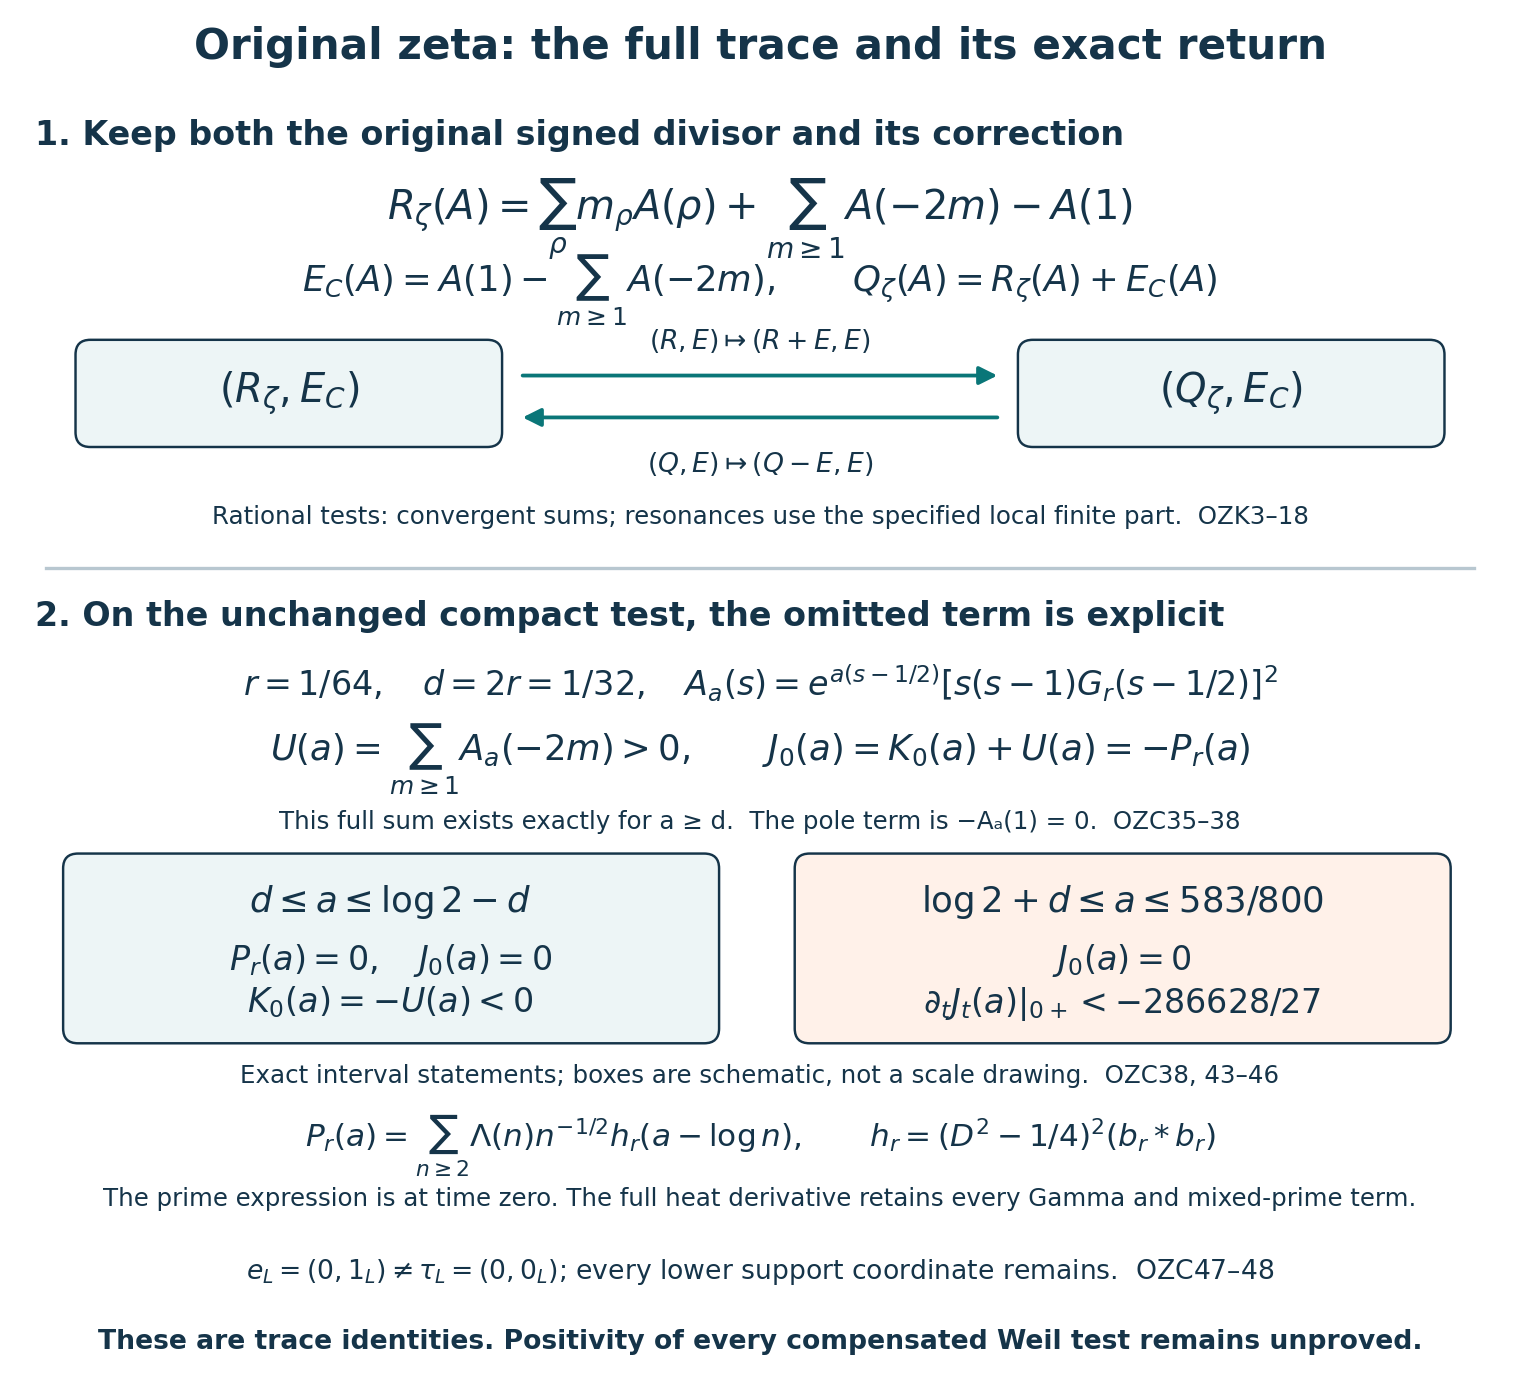
\includegraphics[keepaspectratio,alt={Full signed divisor and faithful return to the Hermitian pairing. The top panel displays OZK3--18, including the inverse retaining the complete correction. The bottom panel is the exact compact-test calculation OZC35--46: the trivial-zero sum equals the earlier archimedean remainder, the pole contribution evaluates to zero, and the full signed trace equals the finite prime expression only at time zero. The negative derivative retains all terms of OZC44--45 and the original Rodgers--Tao heat convention, arXiv:1801.05914v5, equations phidef and htdef. The boxes indicate exact intervals, not sampled values or geometric scale. Lower support labels are retained by OZC47--48. The full proofs define the original density and every test in the diagram.}]{original_zeta_trace_return.png}}
\caption{Full signed divisor and faithful return to the Hermitian
pairing. The top panel displays OZK3--18, including the inverse
retaining the complete correction. The bottom panel is the exact
compact-test calculation OZC35--46: the trivial-zero sum equals the
earlier archimedean remainder, the pole contribution evaluates to zero,
and the full signed trace equals the finite prime expression only at
time zero. The negative derivative retains all terms of OZC44--45 and
the original Rodgers--Tao heat convention, arXiv:1801.05914v5, equations
phidef and htdef. The boxes indicate exact intervals, not sampled values
or geometric scale. Lower support labels are retained by OZC47--48. The
full proofs define the original density and every test in the diagram.}
\end{figure}

\subsection{Original-zeta Gaussian and affine receiving
maps}\label{original-zeta-gaussian-and-affine-receiving-maps-5}

The complete extension OZG1--55 proves that Gaussian convolution of the
test at every positive time makes the original trivial-zero scalar sum
diverge for every real translation. Its admissible replacement retains
each cutoff trace and the Gamma boundary with the identical finite sum
U\_N; OZG20--27 gives both maps and the inverse. The full coefficient
tower, its raw non-Hermitian correction and exact compensated negative
index are OZG28--39. No compact-support prime window is assumed after
smoothing; all prime powers and Gamma terms, with explicit error bounds,
are OZG40--52. This extension acts on the tests while fixing the
original zeta zeros.

The different affine change of the actual original heat family is
OZR1--36. Its multiplier is exp(chi) C(phi)/C, with the full inverse,
exceptional units and local jets. The original generator contains every
q derivative term. The signed divisor comparison is OZR19--24; its
Cauchy logarithmic kernel has an additional growth contribution 2a.
OZR33 proves the exact full negative index after that contribution is
retained. The full support carrier and every lower coordinate are
OZG53--55 and OZR34--36. These are the receiving maps for these
specified extensions; the original preceding test, time and domains
remain those stated in its proof.

\clearpage

\section{Original zeta: heat, signed divisor, contact, and retained
arithmetic
factors}\label{original-zeta-heat-signed-divisor-contact-and-retained-arithmetic-factors}

This calculation starts with the original meromorphic zeta function. It
reconstructs the heat and contact receivers formerly presented through
AG, GC, CH, and RT. Every completion factor and fixed divisor entry
remains explicit. An auxiliary entire product is used for growth
estimates with its return map proved; it does not replace the original
zeta function. No Euler product at nonzero heat time and no positivity
theorem are asserted.

\subsection{1. Original meromorphic family and differential
equation}\label{original-meromorphic-family-and-differential-equation}

Keep the source's exact time and spatial coordinates: \[
\begin{aligned}
\zeta_t(s)&=\frac{8}{C(s)}
\int_0^\infty e^{tu^2}\Phi(u)\cosh((2s-1)u)\,du,\quad \zeta_0=\zeta,\\
C(s)&=\frac{s(s-1)}2\pi^{-s/2}\Gamma(s/2),\\
\Phi(u)&=\sum_{n\ge1}
(2\pi^2n^4e^{9u}-3\pi n^2e^{5u})e^{-\pi n^2e^{4u}},\\
q(s)&=\frac{C'(s)}{C(s)}
=\frac1s+\frac1{s-1}-\frac{\log\pi}2+\frac12\psi(s/2).
\end{aligned}\tag{OZH1}
\] The time-zero equality is Rodgers--Tao's equations hoz, sas, phidef,
and htdef, with their factor \(1/8\) retained. This is a meromorphic
quotient; \(C\) is not a holomorphic unit everywhere. Write
\(E_t=C\zeta_t\) only for the auxiliary entire numerator product.

The integral and all its derivatives converge locally uniformly in
complex \(t,s\). Indeed \(|\Phi(u)|\le K e^{9u-ce^{4u}}\): split
\(\pi n^2e^{4u}\) into equal parts, bound one below by
\((\pi/2)e^{4u}\), and sum the other against \(n^4\). The factors
\(e^{Tu^2+K_1u}\) contributed by compact time and spatial sets, and all
polynomial factors from differentiation, are dominated by the retained
superexponential decay. Twice differentiating in \(s\) multiplies the
integrand by \(4u^2\). Expanding the product derivative therefore proves
the meromorphic identity \[
\boxed{4\partial_t\zeta_t
=\zeta_t''+2q\zeta_t'+(q'+q^2)\zeta_t.}
\tag{OZH2}
\] For \(l_t=\zeta_t'/\zeta_t\), continued meromorphically, \[
\boxed{4\partial_t l_t
=l_t''+2l_tl_t'+2q l_t'+2q'l_t+q''+2qq'.}
\tag{OZH3}
\] On a simply connected zero-free neighborhood first divide (OZH2) by
\(\zeta_t\), obtaining
\(4\partial_t\log\zeta_t=l_t'+l_t^2+2ql_t+q'+q^2\); then differentiate
in \(s\). Meromorphic continuation proves the result without a global
logarithm. Although \(q\) is time independent, its terms in (OZH3) do
not vanish.

Repeated differentiation of the original integral and the Leibniz rule
give \[
\partial_t^n\zeta_t(s)=
\frac1{4^n}\sum_{j=0}^{2n}\binom{2n}{j}
\frac{C^{(j)}(s)}{C(s)}\zeta_t^{(2n-j)}(s).
\tag{OZH4}
\] This is \(4^{-n}C^{-1}\partial_s^{2n}(C\zeta_t)\) expanded with every
factor retained. It is an equality of meromorphic functions at
exceptional points as well.

\subsection{2. Fixed zeros, pole, and local
units}\label{fixed-zeros-pole-and-local-units}

The complete multiplier divisor and its local constants are \[
\begin{aligned}
\operatorname{div}C&=[1]-\sum_{m\ge1}[-2m],\\
C(-2m+h)&=h^{-1}b_m(h),&
b_m(0)&=\frac{(-1)^m2m(2m+1)\pi^m}{m!},\\
C(1+h)&=h\,c(h),&c(0)&=\frac12,\qquad C(0)=-1 .
\end{aligned}\tag{OZH5}
\] Gamma has residue \((-1)^m/m!\) at \(-m\); the argument
\(s/2=-m+h/2\) supplies the factor 2. Multiplying all the other factors
in (OZH1) gives the stated residue. The pole at zero cancels the
explicit factor \(s\), giving \(-1\). Gamma has no zeros, so these are
all divisor points.

For real \(t,s\), \(E_t(s)>0\). Every summand of \(\Phi(u)\) is positive
for \(u\ge0\), since \(2\pi n^2e^{4u}-3>0\), and the cosine-hyperbolic
factor is positive. Consequently \[
\begin{aligned}
\zeta_t(-2m+h)&=h\,v_{m,t}(h),&
v_{m,t}(h)&=E_t(-2m+h)/b_m(h),\\
\zeta_t(1+h)&=h^{-1}v_{1,t}(h),&
v_{1,t}(h)&=E_t(1+h)/c(h),\\
\zeta_t(0)&=-E_t(0)\ne0 .
\end{aligned}\tag{OZH6}
\] The displayed units are nonzero at zero at every real time. Thus all
negative even zeros and the pole at 1 are simple and stationary. The
scalar meromorphic function has no zero or pole at the origin. The
supported prime \(e\) remains in the programme's support carrier; this
scalar statement does not remove it.

The complete jet maps are explicit. If \(E_t(s_0+h)=\sum e_j(t)h^j\) and
\(b(h)^{-1}=\sum d_jh^j\), then \[
[h^n]v_t(h)=\sum_{j=0}^n d_j e_{n-j}(t).
\tag{OZH7}
\] Multiplication by the nonvanishing unit \(b\) is the inverse; at the
pole use \(c\). The original embedded fibers are
\(h\mathcal O/h^2\mathcal O\) at a negative even zero and
\(h^{-1}\mathcal O/\mathcal O\) at the pole, not their images in the
ordinary fiber of \(\mathcal O\).

At a fixed divisor point set \(k=1\) for a zero and \(k=-1\) for the
pole. With the appropriate multiplier unit \(b\), \[
l_t=k/h+v_t'/v_t,\qquad
q=-k/h+b'/b,\qquad
l_t+q=v_t'/v_t+b'/b.
\tag{OZH8}
\] The last expression is holomorphic. The right side of (OZH3) is
therefore holomorphic there, being the spatial derivative of
\(\{(l_t+q)'+(l_t+q)^2\}\). Equivalently
\(\partial_t l_t=\partial_s(\partial_t v_t/v_t)\). This proves that
every fixed divisor residue has derivative zero, while retaining its
unit and all unit derivatives. It proves the cancellations of the
apparent singularities rather than discarding the individual singular
terms.

\subsection{3. Complete signed-divisor traces for rational
tests}\label{complete-signed-divisor-traces-for-rational-tests}

Let \(A\) be rational and \(A(s)=O(s^{-2})\) at infinity. Its poles must
avoid the divisor of \(C\), and the zeros and poles of \(\zeta_{t_*}\),
at a fixed real time \(t_*\). Let \(\mathcal Z_t\) be the zeros of
\(\zeta_t\) away from the fixed negative even zeros, with multiplicities
\(m_{\rho,t}\). For real time these are exactly the zeros of
\(E_t=C\zeta_t\). The full signed trace is \[
\mathcal T_t^\zeta(A)=
\sum_{\rho\in\mathcal Z_t}m_{\rho,t}A(\rho)
+\sum_{m\ge1}A(-2m)-A(1).
\tag{OZH9}
\] Both sums converge absolutely. Substitution \(x=e^{4u}\) in the
estimate of section 1 gives
\(\log\max_{|s|\le R}|E_t(s)|=O_T((R+1)\log(R+2))\). Since
\(E_{t_*}(0)>0\), its value remains bounded away from zero on a small
complex time disc. Jensen's formula gives \(N_t(R)=O(R\log(R+2))\)
uniformly there, and dyadic summation gives
\(\sum_{|\rho|>R}m_{\rho,t}/|\rho|^2=O(\log(R+2)/R)\). The fixed sum is
dominated by \(\sum m^{-2}\).

The digamma series, with its zero pole explicitly cancelled against the
\(1/s\) already present in (OZH1), gives \[
q(s)=\frac1{s-1}-\frac{\gamma+\log\pi}{2}
+\sum_{m\ge1}\left(\frac1{2m}-\frac1{s+2m}\right).
\tag{OZH10}
\] This equality does not replace the original factor formula (OZH1).
Its paired summand is \(s/(2m(s+2m))\), proving normal convergence off
the poles. Hadamard factorization applied to the auxiliary product, with
the growth just verified, gives the original-zeta identity \[
l_t(s)=\beta_t+
\sum_{\rho\in\mathcal Z_t}m_{\rho,t}
\left(\frac1{s-\rho}+\frac1\rho\right)-q(s),\quad
\beta_t=l_t(0)+q(0),\quad
q(0)=-1-\frac{\gamma+\log\pi}{2}.
\tag{OZH11}
\] The two series explicitly retain the trivial zeros and pole. Their
normal convergence follows from the square-denominator bounds.

For the finite test-pole set \(\mathcal P(A)\), \[
\boxed{\mathcal T_t^\zeta(A)=
-\sum_{p\in\mathcal P(A)}\operatorname{Res}_{s=p}(A(s)l_t(s)).}
\tag{OZH12}
\] Indeed a constant times \(A\) has total finite residue zero, since
\(A=O(s^{-2})\). Each moving-zero paired term in (OZH11) contributes
\(A(\rho)\), by the residue theorem for \(A(s)/(s-\rho)\). Each negative
even term in \(-q\) contributes \(A(-2m)\), and its pole term
contributes \(-A(1)\). Normal convergence on circles around the finite
test poles permits termwise residues. All correction constants remain
until their residue is proved zero.

The finite residue expression is holomorphic on a small complex time
disc avoiding zeros at the test poles and gives the analytic
continuation of the real-time full trace. At any complex-time collision
with a fixed divisor point the signed orders add; the meromorphic
identity still gives their sum. Differentiating the finite expression
proves \[
\boxed{
\partial_t\mathcal T_t^\zeta(A)=
-\frac14\sum_{p\in\mathcal P(A)}\operatorname{Res}_{p}
A\{l_t''+2l_tl_t'+2q l_t'+2q'l_t+q''+2qq'\}.}
\tag{OZH13}
\] The complete fixed sum and pole entry in (OZH9) are independent of
time, so their derivative is zero. No interchange with an unrestricted
differentiated moving-zero sum is used.

For \(A_{z,w}(s)=-[(s-(1-\bar z))(s-w)]^{-1}\), whose distinct poles
satisfy the exclusions, direct residue evaluation gives \[
\mathcal T_t^\zeta(A_{z,w})=
\frac{l_t(w)-l_t(1-\bar z)}{w+\bar z-1}.
\tag{OZH14}
\] Its difference from the moving-zero receiver is exactly
\(\sum_m A_{z,w}(-2m)-A_{z,w}(1)\). The actual reflection is \[
l_t(1-s)=-l_t(s)-q(s)-q(1-s),\qquad
\partial_t l_t(1-s)=-\partial_t l_t(s).
\tag{OZH15}
\] Differentiate \(C(1-s)\zeta_t(1-s)=C(s)\zeta_t(s)\), which follows
from the integral's reflection. Thus the original reflected rational
kernel retains both multiplier terms.

\subsection{4. Compact tests and an exact trivial-zero convergence
boundary}\label{compact-tests-and-an-exact-trivial-zero-convergence-boundary}

Use the original transform \[
A(s)=M_h(s)=\int_{\mathbb R}h(v)e^{-(s-1/2)v}\,dv,
\qquad h\in C_c^\infty(\mathbb R).
\tag{OZH16}
\] Integration by parts gives rapid vertical decay on every fixed closed
strip. It does not give decay on the negative real axis: a nonzero
nonnegative \(h\) supported in \([d,2d]\), \(d>0\), has
\(A(-2m)\ge e^{(2m+1/2)d}\int h\). Its trivial-zero sum diverges. Thus
(OZH9) is not a scalar functional on all compact Mellin tests.

The complete object on that larger domain is the indexed divisor record
\[
\mathcal D_t(A)=
\left((m_{\rho,t}A(\rho))_{\rho\in\mathcal Z_t},
(A(-2m))_{m\ge1},-A(1)\right).
\tag{OZH17}
\] For \(t\ge0\) its first component is absolutely summable. The de
Bruijn strip theorem in RT2, with its exact original time, applies to
the real even kernel with the superexponential bound already proved. The
known time-zero strip, under the source coordinate \(Z=-2i(s-1/2)\),
gives \(|\Re\rho_t-\frac12|\le\frac12\sqrt{\max(1-2t,0)}\le\frac12\).
The zero count and the compact-test strip decay prove absolute
summability, uniformly on compact positive-time intervals. No common
strip is asserted for negative or complex time.

Each finite fixed-divisor cutoff is an actual receiving map: \[
\begin{aligned}
\mathcal T_{t,N}^\zeta(A)&=
\sum_{\rho\in\mathcal Z_t}m_{\rho,t}A(\rho)
+\sum_{m=1}^N A(-2m)-A(1),\\
\mathcal T_{t,N}^\zeta(A)-\sum_{m=1}^N A(-2m)+A(1)
&=\sum_{\rho\in\mathcal Z_t}m_{\rho,t}A(\rho).
\end{aligned}\tag{OZH18}
\] The right side is independent of \(N\). This proves the
relative-trace map from the complete record, with its full compensation
exhibited. It does not assert convergence of the uncompensated first
line.

For the fixed primitive test retain exactly \[
\begin{aligned}
r&=1/64,\quad b_r=*_{j\ge1}
\frac{\mathbf1_{[-r2^{-j},r2^{-j}]}}{2r2^{-j}},\quad
G_r(z)=\int b_r(v)e^{-zv}\,dv,\\
F(s)&=s(s-1)G_r(s-1/2),\quad H(s)=F(s)^2,\quad
A_a(s)=e^{a(s-1/2)}H(s).
\end{aligned}\tag{OZH19}
\] UP1--UP10 proves \(b_r\ge0\), smoothness, evenness, mass 1, and
support in \([-r,r]\). Its dyadic construction also proves positive mass
in \([r',r]\) for every \(r'<r\). To see this, the uniformly convergent
sum of independent uniform variables with these radii exists because
their absolute radii sum to \(r\). Its characteristic function is the
defining Fourier product, so its law is \(b_r(v)\,dv\). Choose finitely
many summands so the remaining tail radius is less than \((r-r')/4\),
and restrict each chosen summand to a sufficiently short interval next
to its upper endpoint. This event has positive product probability, and
every permitted tail gives a sum greater than \(r'\). This proves the
endpoint mass assertion for the exact density.

There is an exact convergence boundary: \[
\boxed{\sum_{m\ge1}A_a(-2m)<\infty
\quad\Longleftrightarrow\quad a\ge2r=\frac1{32}
\qquad(a\in\mathbb R).}
\tag{OZH20}
\] All these summands are positive. Put \(R=2m+\frac12\). Flatness at
the endpoints permits repeated integration by parts: \[
|G_r(R)|\le\|b_r^{(N)}\|_{L^1}R^{-N}e^{rR}.
\tag{OZH21}
\] Since \(G_r\) is even, \(A_a(-2m)=(2m)^2(2m+1)^2e^{-aR}G_r(R)^2\).
For \(a\ge2r\) the bound is a constant times \(m^{4-2N}\), summable for
\(N\ge3\). This includes equality. For \(a<2r\), choose \(r'<r\) with
\(2r'>a\). Evenness and positive endpoint mass give
\(G_r(R)\ge c_{r'}e^{r'R}\). The summands then grow at least as a
positive polynomial times \(e^{(2r'-a)R}\), so do not tend to zero. This
proves both directions.

Thus at \(a=0\) the earlier \(K_t(a)\) is the relative trace in (OZH18),
not an absolutely convergent complete-divisor scalar trace. For
\(t\ge0\) and \(a\ge1/32\) its exact relation is \[
\mathcal T_t^\zeta(A_a)=K_t(a)+U(a),\qquad
U(a)=\sum_{m\ge1}(2m)^2(2m+1)^2
e^{-a(2m+1/2)}G_r(2m+1/2)^2>0.
\tag{OZH22}
\] The pole entry is the evaluated zero \(-A_a(1)=0\), because of the
retained test factor \(s(s-1)\). Every \(a\) derivative of \(U\)
converges at and beyond the boundary by (OZH21), after increasing \(N\).
This is an exact comparison function, not a transfer of a positivity
theorem.

\subsection{5. Actual compact-test variation in original
coordinates}\label{actual-compact-test-variation-in-original-coordinates}

Choose \(1<\sigma<3\), so \(1-\sigma\) lies left of the moving strip and
right of the first trivial zero. The original logarithmic derivative
yields \[
\begin{aligned}
Z_t(A)-A(1)=\frac1{2\pi i}\int_{\Re s=\sigma}
\bigl[&
\{A(s)+A(1-s)\}l_t(s)\\
&+A(1-s)\{q(s)+q(1-s)\}\bigr]\,ds,\quad t\ge0 .
\end{aligned}\tag{OZH23}
\] Here \(Z_t\) denotes only the first-component sum in (OZH18). A
rectangle between the two lines contains the pole at 1, of residue
\(-A(1)\), and no trivial zeros. On the left edge the downward
orientation and \(s\mapsto1-s\) give \(-A(1-s)l_t(1-s)\); (OZH15) gives
precisely the displayed integrand.

The convergence and exhaustion can be checked directly with
(OZH10)--(OZH11). On the two lines split their zero sums at
\(|\rho|=2(|s|+1)\). The near part has multiplicity \(O(R\log R)\) and
fixed horizontal distance from the line; the tail retains
\(s/[\rho(s-\rho)]\). Their spatial derivatives have similar bounds.
This gives \(O((1+|\Im s|)^2)\) for each fixed derivative of \(l_t+q\),
uniformly on compact positive-time intervals. The paired series (OZH10)
gives a polynomial bound for each derivative of \(q\) on both lines,
avoiding its poles. Each separate term is therefore integrable against
the arbitrarily rapid strip decay of \(A\).

At height \(j\), choose \(Y_j\in[j,j+1]\) at distance at least
\(j^{-3}\) from adjacent absolute zero ordinates. The excluded length is
\(O(j^{-2}\log j)<1\). The near sums on the horizontal edges then have
polynomial growth, and the paired tails have the previous bounds. The
rapid decay of \(A\) forces the horizontal integrals to zero. This
proves (OZH23) from the residue theorem, with the pole contribution
retained.

Equation (OZH3) and induction give polynomial bounds for every fixed
time derivative on the lines. Dominated integration and the fundamental
theorem of calculus in real time prove that every finite cutoff trace is
\(C^\infty\) for \(t\ge0\), with right derivatives at zero. In
particular \[
\boxed{
\left.\partial_t\mathcal T_{t,N}^\zeta(A)\right|_{0+}
=\frac1{2\pi i}\int_{\Re s=\sigma}
\{A(s)+A(1-s)\}
\frac{l_0''+2l_0l_0'+2q l_0'+2q'l_0+q''+2qq'}4\,ds.}
\tag{OZH24}
\] The finite fixed-divisor entries have zero derivative, so this value
is independent of \(N\). If the full fixed sum converges, its derivative
is the same because its full added value is time independent.

All higher recurrences can likewise retain the two separate types of
jets. In a polynomial algebra use formal \(l_j,q_j\), let
\(Dl_j=l_{j+1}\), \(Dq_j=q_{j+1}\), and set \[
\mathcal B=\tfrac14(l_2+2l_0l_1+2q_0l_1+2q_1l_0+q_2+2q_0q_1),
\qquad Vl_j=D^j\mathcal B,\quad Vq_j=0.
\tag{OZH25}
\] The chain rule proves \(\partial_t^k l_t=V^k l_0\) after evaluating
the spatial jets. For \(k\ge1\) this replaces the quotient in (OZH24).
For \(k=0\), the additional multiplier-reflection and pole terms remain
exactly as in (OZH23). No zeroth-order boundary term is inherited as
zero.

\subsection{6. Contact in original-zeta
units}\label{contact-in-original-zeta-units}

At a moving zero \(\rho\) of multiplicity \(m\), write \[
\zeta(s)=(s-\rho)^m v_\rho(s),\qquad
d_\rho=v_\rho'(\rho)/v_\rho(\rho),\qquad
q_\rho=\frac1\rho+\frac1{\rho-1}-\frac{\log\pi}2+
\frac12\psi(\rho/2).
\tag{OZH26}
\] Both \(C\) and \(v_\rho\) are holomorphic nonzero units near
\(\rho\). Expanding every term of (OZH2) divided by \(\zeta\) gives the
principal part \[
\operatorname{PP}_\rho
\left(\frac{\zeta''}{\zeta}+2q\frac{\zeta'}{\zeta}+q'+q^2\right)
=\frac{m(m-1)}{(s-\rho)^2}
+\frac{2m(d_\rho+q_\rho)}{s-\rho}.
\tag{OZH27}
\] The term \(2q\zeta'/\zeta\) supplies \(2mq_\rho/(s-\rho)\);
\(q'+q^2\) is holomorphic here, not discarded elsewhere.

For \(A\) holomorphic in an isolating disc, \[
\boxed{
\left.\partial_t\right|_0\frac1{2\pi i}
\int_{\partial D_\rho}A(s)l_t(s)\,ds
=-\frac{m(m-1)}4A''(\rho)
-\frac m2(d_\rho+q_\rho)A'(\rho).}
\tag{OZH28}
\] Compact nonvanishing on the contour permits time differentiation.
Differentiate (OZH27) in \(s\), multiply by the Taylor expansion of
\(A\), and take the residue. This proves the cluster formula without
choosing differentiable labels for splitting multiple roots. At a simple
zero it yields \[
\rho'(0)=-\frac{\zeta''(\rho)}{4\zeta'(\rho)}-\frac{q_\rho}{2}
=-\frac{d_\rho+q_\rho}{2}.
\tag{OZH29}
\] Thus the Gamma and endpoint contribution is part of the actual
velocity.

For the fixed primitive tests, the contact sum is \[
\mathcal C(a)=\frac14\sum_\rho m_\rho(m_\rho-1)A_a''(\rho).
\tag{OZH30}
\] It converges absolutely with all real \(a\) derivatives, locally
uniformly in \(a\). The squared multiplicity in a radius-\(R\) annulus
is \(O(R^2\log^2R)\), bounded by the square of its total multiplicity.
Each test derivative decreases faster than any power on the zero strip;
\(a\) derivatives introduce only powers of \(s-\frac12\). These
estimates prove the assertions by dyadic summation. The fixed simple
trivial zeros and pole have zero variation by (OZH8), not a fictitious
moving contact term.

The exact globally grouped expression, for compact Mellin tests, retains
the unit interactions. Put \[
\beta=l_0(0)-1-\frac{\gamma+\log\pi}{2},\qquad
T_A(\rho,\eta)=
\frac{A'(\rho)-A'(\eta)}{\rho-\eta}
+\frac{A'(\rho)}{\eta}+\frac{A'(\eta)}{\rho}.
\tag{OZH31}
\] For the actual right derivative \(\mathcal V(A)\) in (OZH24), \[
\begin{aligned}
\mathcal V(A)+\frac14\sum_\rho m_\rho(m_\rho-1)A''(\rho)
=-\frac12\bigg[&
\beta\sum_\rho m_\rho A'(\rho)
+\sum_\rho\frac{m_\rho^2A'(\rho)}{\rho}\\
&+\sum_{\{\rho,\eta\}}m_\rho m_\eta T_A(\rho,\eta)\bigg].
\end{aligned}\tag{OZH32}
\] The last sum is over unordered distinct moving supports. Taking the
regular part of (OZH11), with \(q\) retained, proves \[
d_\rho+q_\rho=\beta+\frac{m_\rho}{\rho}
+\sum_{\eta\ne\rho}m_\eta
\left(\frac1{\rho-\eta}+\frac1\eta\right).
\tag{OZH33}
\] Its tail is \(O_\rho(m_\eta/|\eta|^2)\). Insert this in (OZH28),
summed over a finite separated contour. The pairs inside combine into
(OZH31).

For completeness all limits here are controlled. For comparable large
moduli, use \(A''\) integrated along the joining segment when the two
supports are close, and rapid endpoint estimates when far. The resulting
divided differences have arbitrarily rapid decay; the pair multiplicity
weight is \(O(R^2\log^2R)\). For \(|\eta|\ge2|\rho|\), the exact
rearrangement \[
T_A(\rho,\eta)=
\frac{\rho A'(\rho)}{\eta(\rho-\eta)}
+\frac{\eta A'(\eta)}{\rho(\eta-\rho)}
\tag{OZH34}
\] is bounded by \(2|\rho||A'(\rho)|/|\eta|^2+
2|A'(\eta)|/|\rho|\). The zero count gives the square tail
\(O(\log R/R)\) and \(\sum_{|\rho|\le R}m_\rho/|\rho|=O(\log^2(R+2))\),
proving absolute convergence. Across the separated contour at height
\(T\), the bounded-height cross terms are \(O(\log T/T)\); those of
moduli comparable to \(T\) are \(O_N(T^{5-N}\log^2T)\), using the
distance \(T^{-3}\); the further tail is \(O_N(T^{1-N}\log^2T)\). These
tend to zero. This proves (OZH32) with its grouped sums and the
derivative already proved in (OZH24). It does not assume convergence of
the ungrouped velocity series. Rational tests instead have their full
derivative defined and proved by (OZH13), without needing this
compact-test exhaustion.

Let \(c_\rho=\rho-\frac12\). For the fixed \(H=F^2\), the Laplace
transform in \(a\), first for \(\Re w>\frac12\), has the exact residual
principal part \[
\boxed{
\operatorname{PP}_{w=c_\rho}\widehat{\mathcal V+\mathcal C}(w)
=-\frac{m_\rho}{2}
\left(d_\rho+\frac1\rho+\frac1{\rho-1}
-\frac{\log\pi}{2}+\frac12\psi(\rho/2)\right)
\left(\frac{F(\rho)^2}{(w-c_\rho)^2}
+\frac{2F(\rho)F'(\rho)}{w-c_\rho}\right).}
\tag{OZH35}
\] To prove it, the Laplace transform of \(A_a(s)\) is
\(H(s)/(w-(s-\frac12))\) on the zero strip. The preceding estimates have
integrable majorant \((1+a^2)e^{-(\Re w-1/2)a}\), so transformation
through every grouped sum is justified. Their tails converge normally on
compact \(w\)-sets avoiding the discrete \(c_\rho\), by the same
divided-difference bounds and high-height denominator bounds. Isolating
the pairs containing \(\rho\) and using (OZH33) gives (OZH35). The
contact contribution removed has principal part \[
\frac{m_\rho(m_\rho-1)}4
\left(\frac{2H(\rho)}{(w-c_\rho)^3}
+\frac{2H'(\rho)}{(w-c_\rho)^2}
+\frac{H''(\rho)}{w-c_\rho}\right).
\tag{OZH35a}
\] This computes all of it, not only its triple pole.

The higher-order original-zeta formula is also exact. At a simple zero
define \[
n_\rho=\min\left\{n\ge1:
\sum_{j=0}^{2n}\binom{2n}{j}
C^{(j)}(\rho)\zeta^{(2n-j)}(\rho)\ne0\right\}.
\tag{OZH36}
\] This minimum is finite: substitution \(x=\sqrt T\,u\) in the original
integral proves
\(\sqrt T\,\zeta_{-T}(\rho)\to4\sqrt\pi\,\Phi(0)/C(\rho)\ne0\) by
dominated convergence, with bound a constant times
\(e^{-x^2+|2\rho-1|x}\). Thus its time-entire value is not identically
zero. Formula (OZH4) identifies its Taylor coefficients. Analytic
division at the simple zero then gives \[
\rho(t)=\rho-
\frac{\sum_{j=0}^{2n_\rho}\binom{2n_\rho}{j}
C^{(j)}(\rho)\zeta^{(2n_\rho-j)}(\rho)}
{4^{n_\rho}n_\rho!\,C(\rho)\zeta'(\rho)}
t^{n_\rho}+O(t^{n_\rho+1}).
\tag{OZH37}
\] The local resolvent's first nonzero time derivative has the same
coefficient without \(n_\rho!\), multiplying
\(\{F(\rho)^2/(w-c_\rho)^2+2F(\rho)F'(\rho)/(w-c_\rho)\}\). All
multiplier derivatives remain in that numerator.

\subsection{7. Original Euler derivative and full causal
arithmetic}\label{original-euler-derivative-and-full-causal-arithmetic}

At time zero on \(\Re s>1\), the original Euler product gives \[
l_0(s)=-P(s),\qquad P(s)=\sum_{n\ge2}\Lambda(n)n^{-s}.
\tag{OZH38}
\] Local uniform convergence and differentiation follow from comparison
with \(\sum(\log n)n^{-\sigma}\), retaining a smaller positive
convergence margin for derivatives. Equation (OZH3) becomes \[
4\partial_t l_t|_0=-P''+2PP'-2qP'-2q'P+q''+2qq'.
\tag{OZH39}
\] Every term is calculated from the original \(\zeta'/\zeta\),
including both cross terms and both pure multiplier terms.

For compact smooth \(\varphi\) define \[
\begin{aligned}
\pi_{\rm ar}&=\sum_{n\ge2}\frac{\Lambda(n)}{\sqrt n}\delta_{\log n},\\
\langle\alpha,\varphi\rangle
&=\int_0^\infty(e^{-v/2}+e^{v/2})\varphi(v)\,dv
-\frac{\gamma+\log\pi}{2}\varphi(0)\\
&\quad+\int_0^\infty
\frac{e^{-2v}\varphi(0)-e^{-v/2}\varphi(v)}
{1-e^{-2v}}\,dv .
\end{aligned}\tag{OZH40}
\] The last numerator near zero is
\(v(-3\varphi(0)/2-\varphi'(0))+O(v^2)\), so the quotient is bounded.
Beyond the compact support the remaining term is integrable. This is a
causal distribution of order at most one. On \(\Re s>1\), substitution
of the exponential test and \(x=2v\) in the last integral gives \[
M_{\pi_{\rm ar}}=P,\qquad
M_\alpha=\frac1s+\frac1{s-1}-\frac{\log\pi}{2}
+\frac12\psi(s/2)=q.
\tag{OZH41}
\] Here the convergent digamma integral is
\(\int_0^\infty(e^{-x}-e^{-zx})/(1-e^{-x})\,dx=\psi(z)+\gamma\). It
proves all endpoint, Gamma, and constant contributions separately.

To define singular convolutions, retain the measures \[
G=-\tfrac12e^{-v/2}\log(1-e^{-2v})\mathbf1_{v>0}\,dv,\qquad
m=e^{v/2}\mathbf1_{v>0}\,dv+\tfrac12G
-\tfrac{\gamma+\log\pi}{2}\delta_0 .
\tag{OZH42}
\] Then \(\alpha=DG+m\) as distributions on the whole real line. Write
\(g\) for the density of \(G\); for \(v>0\),
\(g'+g/2=-e^{-5v/2}/(1-e^{-2v})\), and
\(\int_\varepsilon^\infty e^{-2v}/(1-e^{-2v})\,dv
=e^{\varepsilon/2}g(\varepsilon)\). After integration by parts the
difference of the two cutoff boundary expressions is
\(g(\varepsilon)(e^{\varepsilon/2}\varphi(0)-\varphi(\varepsilon))
=O(\varepsilon|\log\varepsilon|)\to0\). This proves the distribution
equality without a hidden boundary atom.

For every \(c>1/2\), \(G,m,\pi_{\rm ar}\) have finite exponentially
weighted total variation and every polynomial moment with that weight.
Near zero \(g=O(1+|\log v|)\); at infinity \(g=O(e^{-5v/2})\); the prime
contribution is bounded by \(\sum(\log n)n^{-c-1/2}\). Polynomial
moments follow by retaining a smaller positive exponential margin.
Causal convolution of these measures is locally finite because addition
is proper on the causal quadrant over compact sets; its weighted norm is
at most the product of the norms. Define distribution convolutions by
derivatives of these measure convolutions, for instance
\(\alpha*\alpha=D^2(G*G)+2D(G*m)+m*m\). Weighted Fubini proves transform
multiplication, and multiplication by \(v\) transforms to
\(-\partial_s\).

It follows that the full causal receiver of (OZH39) is \[
\boxed{
4\mathfrak J_\zeta=
-v^2\pi_{\rm ar}-v(\pi_{\rm ar}*\pi_{\rm ar})
+2v(\alpha*\pi_{\rm ar})
+v^2\alpha-v(\alpha*\alpha).}
\tag{OZH43}
\] This proves its definition and every coefficient. The fixed
multiplier contributes both its pure terms and its interaction with the
prime measure.

Fourier inversion in the original convention gives \[
\left.\partial_t\mathcal T_{t,N}^\zeta(M_h)\right|_{0+}
=\langle\mathfrak J_\zeta,h(v)+h(-v)\rangle .
\tag{OZH44}
\] For verification, first let the causal distribution be a measure with
finite exponential weight \(e^{-(\sigma-\frac12)v}\). Fourier inversion
and weighted Fubini pair its transform with \(M_h(s)\) to yield
\(h(-v)\), and with \(M_h(1-s)\) to yield \(h(v)\); the exponential
weights cancel in each case. For a derivative of a measure use the
differentiated compact test and its rapid Fourier decay. Every term of
(OZH43) has this derivative-of-measures form by (OZH42), including the
polynomial weights. Equation (OZH24) now proves the result for the
actual right derivative.

Writing \(F_h(v)=h(v)+h(-v)\), with support in \([-R,R]\), the complete
expression is \[
\begin{aligned}
4\langle\mathfrak J_\zeta,F_h\rangle={}&
\langle v^2\alpha-v(\alpha*\alpha),F_h\rangle\\
&-\sum_{2\le n\le e^R}\frac{\Lambda(n)}{\sqrt n}
(\log n)^2F_h(\log n)\\
&+2\sum_{2\le n\le e^R}\frac{\Lambda(n)}{\sqrt n}
\langle\alpha,(v+\log n)F_h(v+\log n)\rangle\\
&-\sum_{2\le k\le e^R}\frac{(\Lambda*\Lambda)(k)}{\sqrt k}
(\log k)F_h(\log k).
\end{aligned}\tag{OZH45}
\] The coefficient
\((\Lambda*\Lambda)(k)=\sum_{mn=k}\Lambda(m)\Lambda(n)\) retains every
ordered factorization. Causality proves the finite cutoffs. This
reconstructs the arithmetic variation from the original Euler derivative
rather than replacing that derivative by a completed one.

\subsection{8. Full lattice labels and receiving
maps}\label{full-lattice-labels-and-receiving-maps}

Let \(L\) be the original finite bounded distributive lattice. Its
carrier is exactly
\(G_L(V)=\{(v,1_L):v\in V\}\cup\{z_\lambda=(0,\lambda):\lambda\ne1_L\}\),
on each stated scalar or linear receiving space. Nonzero amplitudes
occur only at top support. Keep each divisor entry in (OZH17) with its
original index and top support; the lower zero labels remain separate. A
zero amplitude at a present top-supported entry is \((0,1_L)=e\);
absence is \(\tau=z_{0_L}\). A specified linear residue, contour,
differentiation, or finite-cutoff receiver lifts by \[
(U,1_L)\longmapsto(\mathcal F(U),1_L),\qquad
z_\lambda\longmapsto z_\lambda\quad(\lambda\ne1_L).
\tag{OZH46}
\] Linearity of the amplitude map and retention of the join label prove
additivity; the original scalar action retains its meet rule. The
independent complex coefficients \(c_\lambda\) are values of functions
on lower carrier points; they belong to the attached function space and
are retained by the identity there. They are not nonzero amplitudes in
the lower carrier strata. An arbitrary test pairing is not asserted
multiplicative. Causal convolution uses meet labels and the original
ordered indices, before labels over the same product index are joined.
In particular the raw index \(n=1\) retains \(e\), while the sparse
index retains \(\tau\). Their amplitude-zero images are different
labelled objects.

Retain the original supported identity, on its proved test domain, \[
\begin{aligned}
\boldsymbol B_L&=(A(0)+A(1))\mathbf e_{1_L}
+A(0)\sum_{\lambda\ne1_L}\mathbf e_\lambda,\\
\boldsymbol Z_L&=Z_0(A)\mathbf e_{1_L},\\
\boldsymbol D_L&=(P_{\rm fin}-A_\infty)\mathbf e_{1_L}
+A(0)\sum_{\lambda\ne1_L}\mathbf e_\lambda,\qquad
\boldsymbol B_L-\boldsymbol Z_L=\boldsymbol D_L.
\end{aligned}\tag{OZH47}
\] The finite-prime and archimedean functionals have exactly the
original SZW definitions. Their separate original-zeta reconstruction is
the companion OZC calculation; the map here does not suppress them.
Define \[
\begin{aligned}
U_N(A)&=\sum_{m=1}^N A(-2m),\\
\boldsymbol B_{L,N}^\zeta&=\boldsymbol B_L+
\{U_N(A)-A(1)\}\mathbf e_{1_L},\\
\boldsymbol Z_{L,N}^\zeta&=\mathcal T_{0,N}^\zeta(A)\mathbf e_{1_L},\qquad
\boldsymbol B_{L,N}^\zeta-\boldsymbol Z_{L,N}^\zeta
=\boldsymbol D_L.
\end{aligned}\tag{OZH48}
\] Substitution of (OZH18) proves the equality. Store the full indexed
fixed sequence as well as these finite receiving maps. When it
converges, absolute convergence gives the corresponding full-sum map.
The \(A(0)\) coordinate and every lower lattice coordinate remain; this
states precisely how the supported-zero prime is retained when the
scalar zeta divisor has no point at zero.

For fixed tests, in the induced time-dependent identity, \[
\dot{\boldsymbol B}_{L,N}^\zeta=0,\qquad
\dot{\boldsymbol Z}_{L,N}^\zeta=\mathcal V(A)\mathbf e_{1_L},\qquad
\dot{\boldsymbol D}_{L,N}^\zeta=-\mathcal V(A)\mathbf e_{1_L}.
\tag{OZH49}
\] All fixed divisor, endpoint, and lower support coordinates have their
calculated zero derivative with labels retained. Adding contact changes
the last two entries by \(+\mathcal C\,\mathbf e_{1_L}\) and
\(-\mathcal C\,\mathbf e_{1_L}\). The original heat equation remains
(OZH2); the trace correction does not construct a different
persistent-contact heat family.

These calculations retain the previously obtained first-variation
numbers on their proved domains, reconstruct their local drift with all
original-zeta and multiplier terms, and restore the full fixed divisor
record. The additional boundary (OZH20) proves that the old zero-strip
correlation at the origin is a relative trace and cannot be called an
absolutely convergent complete-divisor sum.

\subsection{Sources and actual
reading}\label{sources-and-actual-reading}

The original author source is Brad Rodgers and Terence Tao, \emph{The de
Bruijn--Newman constant is non-negative},
\href{https://arxiv.org/src/1801.05914v5}{arXiv:1801.05914v5 author
TeX}. Its file fmp-template.tex, lines 64--153, was read for this
calculation, including hoz, sas, phidef, htdef and the heat equation.
This is bounded reading, not a claim to have reread the entire paper.

The complete programme proofs read are AG1--AG24, GC1--GC31a, CH1--CH30,
and RT1--RT30. Their SHA256 values, in that order, are:

\begin{itemize}
\tightlist
\item
  \texttt{00b2bc42\allowbreak{}ab649558\allowbreak{}e7af9c8c\allowbreak{}781bdb4d\allowbreak{}3b08f43b\allowbreak{}cfd496fe\allowbreak{}6f9e6e0f\allowbreak{}a453a4b0}
\item
  \texttt{589c5b42\allowbreak{}c3bf2ad6\allowbreak{}3c5370f8\allowbreak{}9eb36e72\allowbreak{}72b28c04\allowbreak{}08d460f0\allowbreak{}41ccd120\allowbreak{}60b4e27b}
\item
  \texttt{6fed48dd\allowbreak{}0eb9e4ce\allowbreak{}335d3b84\allowbreak{}532d2117\allowbreak{}bc234937\allowbreak{}06309123\allowbreak{}58439003\allowbreak{}aae35de1}
\item
  \texttt{aa783421\allowbreak{}f559bba4\allowbreak{}ba123bbf\allowbreak{}fba18e2c\allowbreak{}0336bcbc\allowbreak{}ccd2aec8\allowbreak{}65892df6\allowbreak{}f50983ae}
\end{itemize}

UP0--UP18 was reread for the density and product. The classical bump
attribution remains Juan Arias de Reyna, \emph{An infinitely
differentiable function with compact support: Definition and
properties}, arXiv:1702.05442v1, Theorem 1; its dyadic constants are
unchanged. The de Bruijn theorem is used exactly as quoted in RT2:
Alexander Dobner, arXiv:2005.05142v2, author file paper.tex, theorem
debruijnthm, citing N. G. de Bruijn (1950), Theorem 13. This derivation
has not independently reread those latter author sources; section 4
verifies the same hypotheses for the exact kernel.

OZH1--OZH15 reconstruct AG's full rational receiver; OZH16--OZH25
reconstruct RT's compact-test domain and prove the new trivial-zero
boundary; OZH26--OZH37 reconstruct GC's contact and local higher-motion
receiver; OZH38--OZH45 reconstruct CH from the original Euler
derivative; OZH46--OZH49 prove the labelled receiving maps. The
companion UZ source supplies the compatible embedded line-module and
all-jet multiplier description. These results do not supply the
unresolved uniform positivity bound for RH.

\subsection{Original-zeta Gaussian and affine receiving
maps}\label{original-zeta-gaussian-and-affine-receiving-maps-6}

The complete extension OZG1--55 proves that Gaussian convolution of the
test at every positive time makes the original trivial-zero scalar sum
diverge for every real translation. Its admissible replacement retains
each cutoff trace and the Gamma boundary with the identical finite sum
U\_N; OZG20--27 gives both maps and the inverse. The full coefficient
tower, its raw non-Hermitian correction and exact compensated negative
index are OZG28--39. No compact-support prime window is assumed after
smoothing; all prime powers and Gamma terms, with explicit error bounds,
are OZG40--52. This extension acts on the tests while fixing the
original zeta zeros.

The different affine change of the actual original heat family is
OZR1--36. Its multiplier is exp(chi) C(phi)/C, with the full inverse,
exceptional units and local jets. The original generator contains every
q derivative term. The signed divisor comparison is OZR19--24; its
Cauchy logarithmic kernel has an additional growth contribution 2a.
OZR33 proves the exact full negative index after that contribution is
retained. The full support carrier and every lower coordinate are
OZG53--55 and OZR34--36. These are the receiving maps for these
specified extensions; the original preceding test, time and domains
remain those stated in its proof.

\clearpage

\section{Original zeta, the complete Cauchy correction, and the
reflected
index}\label{original-zeta-the-complete-cauchy-correction-and-the-reflected-index}

This calculation starts with the meromorphic function \(\zeta\), its
signed divisor, and the original rational tests. Its raw divisor pairing
is generally not Hermitian. The fixed Gamma and endpoint divisor
supplies an explicitly retained correction. The correction, together
with the original pairing, reconstructs the Cauchy--Weil form and all
its finite-jet and exterior blocks. At the previously admissible real
poles \(\sigma=3,5,\ldots\), the reflected test has a pole at a trivial
zero. Ordinary evaluation there is undefined. We give an extension in
the original local coordinate, prove its residue formula with the full
local units, and calculate its difference from a parameter finite part.

The earlier CK, NI and FJ results apply to the compensated receiver
proved below. They do not assign a positive or negative index to the
uncorrected original-zeta pairing. No Riemann-hypothesis sign is proved
here.

\subsection{1. Original function, factors, and test
domains}\label{original-function-factors-and-test-domains}

Retain all factors \[
C(s)=\tfrac12s(s-1)\pi^{-s/2}\Gamma(s/2),\qquad
r(s)=\frac{\zeta'(s)}{\zeta(s)},\qquad
q(s)=\frac1s+\frac1{s-1}-\frac12\log\pi+\frac12\psi(s/2).
\tag{OZK1}
\] The products and quotients are meromorphic identities. In particular
the Gamma pole and polynomial zero at 0 remain separate factors even
though their product is a unit there. The precise local units and
fractional lattices are UZ6--UZ24, read in full for this calculation.
They prove \[
\operatorname{div}C=[1]-\sum_{m\ge1}[-2m],\qquad
\operatorname{div}\zeta=\sum_{\rho\in\mathcal Z}m_\rho[\rho]
 +\sum_{m\ge1}[-2m]-[1].
\tag{OZK2}
\] Here \(\mathcal Z\) consists of distinct nontrivial zeros, with their
original positive multiplicities. The sums of divisors are locally
finite. The actual zero estimate is
\(\sum_{|\rho|>R}m_\rho/|\rho|^2=O(\log(R+2)/R)\), by AG1--AG5. Nothing
in (OZK2) identifies supported zero with either a complex coordinate or
the unsupported element.

Let \(\mathscr A\) be the space of rational functions \(A(s)=O(s^{-2})\)
at infinity whose finite poles avoid \(\mathcal Z\). The subspace
\(\mathscr A^\circ\) also excludes poles at \(1,-2,-4,\ldots\). On this
latter domain the ordinary signed-divisor trace and the
completion-divisor trace are \[
\begin{aligned}
R_\zeta(A)&=\sum_\rho m_\rho A(\rho)+\sum_{m\ge1}A(-2m)-A(1),\\
E_C(A)&=A(1)-\sum_{m\ge1}A(-2m),\\
Q_\zeta(A)&=R_\zeta(A)+E_C(A)=\sum_\rho m_\rho A(\rho).
\end{aligned}\tag{OZK3}
\] All sums converge absolutely: the nontrivial sum uses the displayed
zero estimate, the real sum has tail \(O(m^{-2})\), and the omitted
bounded region contains finitely many points. The last equality is a
calculation with both retained divisor terms. It is not permission to
delete either of them.

For \(\Re z,\Re w>1\), the original Cauchy tests are \[
F_z(s)=(s-z)^{-1},\quad
F^\#(s)=\overline{F(1-\bar s)},\quad
A_{z,w}(s)=F_z^\#(s)F_w(s)
=-\frac1{(s-(1-\bar z))(s-w)}.
\tag{OZK4}
\] Their poles avoid \(\mathcal Z\). They belong to \(\mathscr A^\circ\)
exactly when \(z\notin\{3,5,7,\ldots\}\); the other pole \(w\) cannot be
a fixed divisor point on this domain. The original single-pole algebra
and all its powers are \[
\mathcal R_\sigma=\operatorname{span}_{\mathbb C}\{Q_j:j\ge0\},
\quad Q_j(s)=(s-\sigma)^{-j-1},\quad \sigma>1,
\quad A_{jk}=Q_j^\#Q_k.
\tag{OZK5}
\] They are proper rational functions; each product \(A_{jk}\) belongs
to \(\mathscr A\). We retain every \(\sigma>1\), including resonant odd
integers.

\subsection{2. Defined finite parts at the resonant poles, with every
unit}\label{defined-finite-parts-at-the-resonant-poles-with-every-unit}

For a meromorphic germ in the fixed coordinate \(h=s-a\), define
\(\operatorname{FP}_a A=[h^0]A(a+h)\). This is the constant Laurent
coefficient, not a value of a function with a pole. For a meromorphic
function \(f\) which is not identically zero, write its unique local
factorization in this coordinate as \[
f(a+h)=h^{n_a}u_{f,a}(h),\quad u_{f,a}(0)\ne0,\qquad
\frac{f'}f=\frac{n_a}{h}+\frac{u_{f,a}'}{u_{f,a}}.
\tag{OZK6}
\] If \(A=\sum_{k=-p}^\infty a_kh^k\) and
\(u_{f,a}'/u_{f,a}=\sum_{l\ge0}b_lh^l\), direct multiplication gives \[
\operatorname{Res}_a(Af'/f)
=n_a a_0+\sum_{l=0}^{p-1}a_{-l-1}b_l.
\tag{OZK7}
\] Thus its divisor contribution and its regular-unit contribution are
different specified functionals of the same germs. On a bounded contour
enclosing finitely many divisor points and test poles, subtracting the
second term of (OZK7) at each test pole from the full
logarithmic-derivative integral yields the sum of
\(n_a\operatorname{FP}_aA\). This proves a local-contour definition of
the extension; it does not interpret undefined ordinary evaluation as a
scalar.

In particular at \(a=-2m\), \(m\ge1\), UZ12--UZ14 gives the complete
unit \[
\begin{aligned}
C(a+h)&=h^{-1}c_m(h),\\
c_m(h)&=\kappa_m\left(1-\frac h{2m}\right)
\left(1-\frac h{2m+1}\right)\pi^{-h/2}\Gamma(1+h/2)
\prod_{l=1}^{m}\left(1-\frac h{2l}\right)^{-1},\\
\kappa_m&=(-1)^m\frac{2m(2m+1)\pi^m}{m!},\qquad
\zeta(a+h)=h\,u_m(h).
\end{aligned}\tag{OZK8}
\] Both \(u_m\) and \(c_m\) are units. The analytic product is
\(C\zeta=c_mu_m\), not the product of two scalar fibre values. Hence \[
r(a+h)=h^{-1}+u_m'/u_m,\quad
q(a+h)=-h^{-1}+c_m'/c_m,\quad
r+q=(c_mu_m)'/(c_mu_m).
\tag{OZK9}
\] At 1, with \(h=s-1\), the corresponding factors are
\(\zeta=h^{-1}u_1\), \(C=h c_1\),
\(c_1(h)=\tfrac12(1+h)\pi^{-(1+h)/2}\Gamma((1+h)/2)\), \(u_1(0)=1\),
\(c_1(0)=1/2\). The orders are \(-1,+1\), and the two regular-unit
logarithmic derivatives again add. At zero the whole unit is
\(C(h)=(h-1)\pi^{-h/2}\Gamma(1+h/2)\), with value \(-1\). These
equations preserve all Gamma and endpoint contributions.

Extend (OZK3) to \(\mathscr A\) by replacing each fixed-point evaluation
with its just-defined finite part: \[
\begin{aligned}
R_\zeta^{\rm fp}(A)&=\sum_\rho m_\rho A(\rho)
 +\sum_{m\ge1}\operatorname{FP}_{-2m}A-\operatorname{FP}_1A,\\
E_C^{\rm fp}(A)&=\operatorname{FP}_1A
 -\sum_{m\ge1}\operatorname{FP}_{-2m}A,\\
Q_\zeta(A)&=R_\zeta^{\rm fp}(A)+E_C^{\rm fp}(A).
\end{aligned}\tag{OZK10}
\] Only finitely many summands differ from ordinary evaluations, so
absolute convergence persists. The identities (OZK7)--(OZK9) prove that
the two original logarithmic-derivative contour calculations add with
all their unit terms. The full unit is required for this calculation
even though the signed-divisor receiver afterwards records only the
order and constant Laurent coefficient.

A useful global residue expression makes the extra collision term
explicit. Write \(\mathcal P(A)\) for the test poles and
\(n_f(a)=\operatorname{ord}_a f\). For \(f=\zeta,C\), \[
T_f^{\rm fp}(A)
=-\sum_{a\in\mathcal P(A)}\operatorname{Res}_a(Af'/f)
+\sum_{a\in\mathcal P(A)}n_f(a)\operatorname{FP}_aA.
\tag{OZK11}
\] Here \(T_\zeta=R_\zeta\), \(T_C=E_C\). To prove this globally,
differentiating the reciprocal Gamma product of UZ6 gives the normally
convergent expansion \[
q(s)=\frac1{s-1}-\frac{\gamma+\log\pi}{2}
 +\sum_{m\ge1}\left(\frac1{2m}-\frac1{s+2m}\right).
\tag{OZK12}
\] The \(1/s\) term of (OZK1) and the \(-1/s\) term from Gamma are
accounted for by this derived equality. For \(r+q\), AG7 supplies a
normally convergent genus-one expansion over \(\mathcal Z\). Subtracting
(OZK12) supplies the expansion for the original \(r\), with its pole at
1, all trivial zeros, all nontrivial zeros, and its constant. Constant
terms contribute zero to
\(\sum_{a\in\mathcal P(A)}\operatorname{Res}_a A\). For each divisor
point not in the test pole set, the residues of \(A(s)/(s-x)\) at the
test poles sum to \(-A(x)\). For a point inside that pole set they sum
to zero, since they then include all finite poles and the rational
function has zero residue at infinity. The added term in (OZK11)
restores exactly its specified constant Laurent coefficient. Normal
convergence on finitely many small circles justifies every residue
interchange. At resonant points the last two collision terms for
\(\zeta,C\) cancel because their orders are opposite, and their complete
local units add as in (OZK9).

\subsection{3. Exact raw kernel and complete correction
matrix}\label{exact-raw-kernel-and-complete-correction-matrix}

Set \(a=1-\bar z\), \(d_{z,w}=w+\bar z-1=w-a\). At a nonresonant point,
evaluation of the two test residues in (OZK11) gives \[
\begin{aligned}
R_\zeta(A_{z,w})&=\frac{r(w)-r(a)}{w-a},\\
E_C(A_{z,w})&=\frac{q(w)-q(a)}{w-a}
=A_{z,w}(1)-\sum_{m\ge1}A_{z,w}(-2m),\\
Q_\zeta(A_{z,w})&=
\frac{r(w)+q(w)-r(a)-q(a)}{w-a}.
\end{aligned}\tag{OZK13}
\] The original functional equation gives
\((r+q)(1-\bar z)=-\overline{(r+q)(z)}\). Consequently the last line
equals the earlier CK kernel, but now with every original derivative
term retained as \[
Q_\zeta(A_{z,w})=
\frac{\zeta'(w)/\zeta(w)+\overline{\zeta'(z)/\zeta(z)}
+q(w)+\overline{q(z)}}{w+\bar z-1}.
\tag{OZK14}
\] The separate raw term in (OZK13) uses \(r(1-\bar z)\), not its
unsupported replacement by \(-\overline{r(z)}\).

At \(a=-2m\), write \(r(a+h)=h^{-1}+r_a^{\rm reg}(h)\),
\(q(a+h)=-h^{-1}+q_a^{\rm reg}(h)\), as calculated in (OZK9). Formula
(OZK11) gives instead \[
R_\zeta^{\rm fp}(A_{z,w})
=\frac{r(w)-r_a^{\rm reg}(0)}{w-a},\qquad
E_C^{\rm fp}(A_{z,w})
=\frac{q(w)-q_a^{\rm reg}(0)}{w-a}.
\tag{OZK15}
\] For verification, the direct test constant at that point is
\(\operatorname{FP}_a A_{z,w}=(w-a)^{-2}\). In the residue sum this
cancels the extra \(-(w-a)^{-2}\) arising from the pole of \(r\), while
the two signs reverse for \(q\). Their sum in (OZK15) is (OZK14). Thus
all original real Cauchy poles are included by a defined calculation.

Now fix \(\sigma>1\), put \(d=2\sigma-1\), and define
\(R_{jk}=R_\zeta^{\rm fp}(A_{jk})\), \(E_{jk}=E_C^{\rm fp}(A_{jk})\),
\(C_{jk}=R_{jk}+E_{jk}\). The exact correction in the original power
basis is \[
\begin{aligned}
D_{jk}(\sigma)&:=R_{jk}-C_{jk}=-E_{jk}\\
&=\sum_{m\ge1} b_{m,jk}(\sigma)
 -\frac1{(-\sigma)^{j+1}(1-\sigma)^{k+1}},\\
b_{m,jk}(\sigma)&=
\frac1{(2m+1-\sigma)^{j+1}(-2m-\sigma)^{k+1}}
\quad (\sigma\ne2m+1),\\
b_{m,jk}(2m+1)&=
\frac{(-1)^{j+k}}{(4m+1)^{j+k+2}}
\binom{j+k+1}{j+1}.
\end{aligned}\tag{OZK16}
\] Every index is an integer \(j,k\ge0\); no factorial is suppressed. At
a resonant point, \(A_{jk}(a+h)=(-1)^{j+1}h^{-j-1}(-d+h)^{-k-1}\). The
binomial series for the last factor shows its constant coefficient is
the term with power \(h^{j+1}\), precisely the last line. The remaining
series has tail \(O(m^{-j-k-2})\), proving convergence.

This correction cannot be assigned an inertia as if it were Hermitian.
For every real nonresonant \(\sigma>1\), direct subtraction gives the
strict result \[
R_{01}-R_{10}=D_{01}-D_{10}
=\sum_{m\ge1}\frac{4m+1}
 {(2m+1-\sigma)^2(2m+\sigma)^2}
+\frac1{\sigma^2(\sigma-1)^2}>0.
\tag{OZK17}
\] Indeed \(A_{01}(x)-A_{10}(x)=(1-2x)/((1-x-\sigma)^2(x-\sigma)^2)\).
At \(-2m\) this is positive; subtracting its value at 1 adds the final
positive term. The compensated \(C_{01}=C_{10}\) is real. Thus the full
raw original-zeta matrix is genuinely non-Hermitian in this original
basis. A negativity claim for that raw form cannot be substituted for
Weil negativity.

Finite part in the original variable and finite part in the moving pole
parameter are also different. At \(a=-2m\), use the antiholomorphic
coordinate \(X=\bar z-\sigma\), with real base \(\sigma=2m+1\), so
\(z=\sigma+\bar X\); its divisor summand is \(-X^{-1}(a-w)^{-1}\), whose
constant coefficient in \(X\) is zero. Its direct \(s\)-coordinate
finite part at \(X=0\) is \((w-a)^{-2}\). For the whole basis, direct
\(s\)-finite-part entry minus the nonnegative \((X,Y)\) Laurent
coefficient, with \(Y=w-\sigma\), equals the last line of (OZK16). The
raw kernel has a parameter pole there and is not assigned a convergent
Taylor expansion at that pole. In contrast \(R+E\) has its singular
terms cancelled by the proved identities (OZK9), (OZK15), and has the
holomorphic parameter germ (OZK14).

The passage retaining both original quantities is the invertible
triangular map \[
(R,E)\longmapsto(R+E,E),\qquad
(Q,E)\longmapsto(Q-E,E).
\tag{OZK18}
\] It acts entrywise on every finite matrix and on the entire
coefficient tower. Keeping only \(Q\) would have a kernel; (OZK18) keeps
the original correction as an independent component and has the
displayed inverse.

\subsection{4. Reconstructed coefficient tower with full arithmetic
derivatives}\label{reconstructed-coefficient-tower-with-full-arithmetic-derivatives}

On \(\sigma>1\) the Euler product gives the absolutely convergent
derivative series \[
\begin{aligned}
r_n&=\frac{r^{(n)}(\sigma)}{n!}
=\frac{(-1)^{n+1}}{n!}\sum_{l\ge2}\Lambda(l)(\log l)^n l^{-\sigma},\\
q_n&=\frac{q^{(n)}(\sigma)}{n!}
=(-1)^n\left(\sigma^{-n-1}+(\sigma-1)^{-n-1}\right)
-\mathbf1_{n=0}\frac{\log\pi}{2}
+\frac{\psi^{(n)}(\sigma/2)}{2^{n+1}n!},\qquad \ell_n=r_n+q_n.
\end{aligned}\tag{OZK19}
\] The series may be differentiated on compact subsets of \(\Re s>1\),
using uniform domination by
\(\sum\Lambda(l)(\log l)^n l^{-1-\epsilon}\). Expanding only the now
proved compensated germ gives \[
\begin{aligned}
C_{jk}={}&\sum_{n=0}^{j}(r_n+q_n)
\frac{(-1)^{j+k-n}\binom{j+k-n}{k}}{d^{j+k-n+1}}\\
&+\sum_{n=0}^{k}(r_n+q_n)
\frac{(-1)^{j+k-n}\binom{j+k-n}{j}}{d^{j+k-n+1}}.
\end{aligned}\tag{OZK20}
\] This follows from the geometric denominator series of (OZK14) at
\(z=w=\sigma\), retaining the two occurrences of the constant numerator
coefficient. The coefficients of the rational tests are \(Q_j\) because
\((s-\sigma-Y)^{-1}=\sum_{j\ge0}Y^jQ_j(s)\). The square-summable zero
tail and the distance from \(\sigma\) to the critical strip justify
termwise parameter derivatives of the compensated zero sum. Equations
(OZK16), (OZK19), (OZK20) compute \(R,E,C\) independently of undefined
raw Taylor coefficients at resonances.

For example, the full first determinant is \[
\det(R_{jk}+E_{jk})_{0\le j,k\le1}
=\frac{4(r_0+q_0)^2-d^2(r_1+q_1)^2}{d^4}.
\tag{OZK21}
\] This is obtained from entries \(C_{00}=2\ell_0/d\),
\(C_{01}=C_{10}=\ell_1/d-2\ell_0/d^2\),
\(C_{11}=-2\ell_1/d^2+4\ell_0/d^3\). The raw determinant \(\det R\) is a
different determinant. All larger determinants are those of the
explicitly specified entry sums, not the sum of separate determinants.

\subsection{5. Exact indices and full jets, reconstructed from the
original
trace}\label{exact-indices-and-full-jets-reconstructed-from-the-original-trace}

Let \(\mathcal H=\ell^2(\mathcal Z,m)\), with its conjugate-linear-first
inner product, and let \((Jv)_\rho=v_{1-\bar\rho}\). The original
functional equation, with its multiplier (OZK1), proves equality of the
paired multiplicities and \(J^*=J=J^{-1}\). Direct substitution in
(OZK10) gives \[
R_\zeta^{\rm fp}(F^\#G)+E_C^{\rm fp}(F^\#G)
=\langle J\operatorname{ev}F,\operatorname{ev}G\rangle_{\mathcal H},
\qquad (\operatorname{ev}F)_\rho=F(\rho).
\tag{OZK22}
\] Every critical-line point contributes one positive direction. On a
distinct exchanged pair of weight \(m\), the vectors
\((\delta_\rho\pm\delta_{\rho^\#})/\sqrt{2m}\) have signs \(+1,-1\).
Denote the counts of these signs by \(\kappa_+,\kappa_-\); they count
distinct reflected supports, not multiplicity sums.

For completeness, the evaluation range of the original powers is dense.
If \(h\in\mathcal H\) is orthogonal to every \((\rho-\sigma)^{-j-1}\),
its Cauchy transform \(\sum_\rho m_\rho\bar h_\rho/(\rho-z)\) converges
normally away from the discrete zero set. On a compact \(|z|\le M\), its
tail after \(|\rho|>R>2M+1\) is bounded by
\(2(\sum_{|\rho|>R}m_\rho|h_\rho|^2)^{1/2}(\sum_{|\rho|>R}m_\rho/|\rho|^2)^{1/2}\).
All its derivatives vanish at \(\sigma\), so the identity theorem on the
connected complement of the zero set makes it identically zero there.
Its residue at \(\rho\) is \(-m_\rho\bar h_\rho\), proving \(h=0\). If
any finite initial set of powers is deleted, the same argument makes the
transform a polynomial near \(\sigma\), then throughout its domain; its
residues still vanish. The identical argument works for Cauchy poles in
any set with an accumulation point in \(\Re z>1\). The compensated
extension (OZK15) includes any resonant poles of such a set.

Each finite negative orthonormal family in \(\mathcal H\) can be
approximated by evaluation vectors so closely that its Gram matrix
remains negative definite. In detail, for an isometric negative column
operator \(U:\mathbb C^n\to\mathcal H\), an approximating column
operator \(V\) with \(\|V-U\|<1/4\) satisfies
\(V^*JV\le(-1+2\|V-U\|+\|V-U\|^2)I<-7I/16\). Conversely a negative
subspace injects into the negative spectral space of \(J\), because a
vector with zero negative projection has nonnegative value. This proves
both inequalities in \[
\begin{aligned}
\sup_{N\ge J_0}n_\pm((R_{jk}+E_{jk})_{J_0\le j,k\le N})&=\kappa_\pm
\quad(J_0\ge0),\\
\mathrm{RH}&\Longleftrightarrow
(R_{jk}+E_{jk})_{0\le j,k\le N}\succeq0
\text{ for every }N\ge0.
\end{aligned}\tag{OZK23}
\] The plus-index proof uses positive orthonormal vectors and the bound
\(1-2\|V-U\|-\|V-U\|^2>7/16\). A finite list of approximants uses a
common finite number of powers, proving the finite-section claims. For
finite \(\kappa_-\) some finite section attains it and all larger
sections retain it. For infinite \(\kappa_-\), these finite negative
indices are unbounded. No universal finite decision cutoff follows. This
proves the CK and NI index statements on the reconstructed original-zeta
receiver, while (OZK17) prevents applying them to raw \(R\).

All nontrivial local algebras are literally the same ideals in their
original stalks: \[
\mathcal O_\rho/(\zeta)_\rho
=\mathcal O_\rho/(C\zeta)_\rho
\simeq\mathbb C[v]/(v^{m_\rho}),\qquad v=s-\rho,
\tag{OZK24}
\] because \(C\) is a unit at every \(\rho\in\mathcal Z\). This is a
proof about ideals, not an assertion that units have no derivatives. In
these algebras multiplication by \(a_0+a_1v+\cdots\) has trace
\(m_\rho a_0\), and the reflected coefficient map is
\(a_{\rho,k}\mapsto(-1)^k\overline{a_{\rho^\#,k}}\). Define the algebra
of all local jets whose constant vector is in \(\mathcal H\). Its
evaluation map onto \(\mathcal H\) has the constant section and kernel
\(\mathcal N=\prod_\rho(v)\mathbb C[v]/(v^{m_\rho})\). The compensated
multiplication-trace form is (OZK22), with radical exactly
\(\mathcal N\). Indeed its constant quotient is nondegenerate and every
higher coefficient has zero multiplication trace. Moreover
\(\mathcal N^r=\prod_\rho(v^r)\mathbb C[v]/(v^{m_\rho})\),
\(\bigcap_r\mathcal N^r=0\), and the algebra is the inverse limit of
these quotients: each finite local component stabilizes once
\(r\ge m_\rho\), while the constant vector is already fixed at \(r=1\).
The full raw receiver has the additional fixed-divisor data in (OZK10),
which are not elements of this nontrivial-zero quotient.

\subsection{6. Finite prescribed jets and every complementary
block}\label{finite-prescribed-jets-and-every-complementary-block}

Take a finite reflection-stable \(S\subset\mathcal Z\), with retained
orders \(r_a=r_{a^\#}\ge1\), and let \[
\begin{aligned}
P_S(s)&=\prod_{a\in S}(s-a)^{r_a},\quad d_S=\sum_{a\in S}r_a,
\quad W_S(s)=P_S(s)/(s-\sigma)^{d_S},\\
j_SF&=(\sum_{k<r_a}F^{(k)}(a)v_a^k/k!)_{a\in S},\qquad
\mathcal J_S=\bigoplus_{a\in S}\mathbb C[v_a]/(v_a^{r_a}).
\end{aligned}\tag{OZK25}
\] The map is onto: for jets \(f\), the Chinese remainder theorem gives
a unique polynomial \(N_f\) of degree below \(d_S\) with
\(N_f\equiv(s-\sigma)^{d_S}f_a(s-a)\pmod{(s-a)^{r_a}}\). Then
\(N_f/(s-\sigma)^{d_S}\) is a proper rational section. Divisibility of
the numerator proves \(\ker j_S=W_S\mathcal R_\sigma\). On
\(\mathcal Z\setminus S\), both \(W_S\) and its inverse are bounded:
they approach 1 at infinity and have no zeros or poles on the finitely
many remaining supports in any bounded region. Hence the
Cauchy-transform proof in Section 5 proves that exterior evaluations of
this exact kernel are dense. Adding the section shows that
\((j_SF,F|_{\mathcal Z\setminus S})\) has dense image in
\(\mathcal J_S\oplus\ell^2(\mathcal Z\setminus S,m)\), with its first
coordinate achieved exactly.

Put \(B_S(f,g)=\sum_{a\in S}m_a\bar f_{a^\#,0}g_{a,0}\). For any
specified Hermitian matrix \(H\) on these finite jets, the reconstructed
whole form is exactly \[
R_\zeta^{\rm fp}(F^\#G)+E_C^{\rm fp}(F^\#G)+H(j_SF,j_SG)
=(B_S+H)(j_SF,j_SG)
 +\langle J_{\rm ext}F|_{\rm ext},G|_{\rm ext}\rangle.
\tag{OZK26}
\] Consequently its negative index is
\(\kappa_{{\rm ext},-}+n_-(B_S+H)\), and its positive index is
\(\kappa_{{\rm ext},+}+n_+(B_S+H)\). To prove equality rather than
merely an upper bound, approximate any finite definite spectral family
of the bounded direct-sum operator \(A=(B_S+H)\oplus J_{\rm ext}\) by
the just-proved dense rational image. The error in its Gram matrix is at
most \(\|A\|(2\|U\|\|V-U\|+\|V-U\|^2)\), which can be made less than
half its least definite eigenvalue. The upper bound follows from
injection into the corresponding spectral subspace. This includes all
higher local coefficients, which may enter \(H\), and the full exterior
sign count.

The original raw form on the left without \(E_C\) instead equals the
right side minus \(E_C(F^\#G)\). The latter is an infinite fixed-divisor
correction and is generally not Hermitian. It cannot be represented by
changing only the finite local block \(B_S\).

For a finite coefficient matrix split into any two specified sets of
indices, retain each block \(R_{ab}\), \(E_{ab}\),
\(C_{ab}=R_{ab}+E_{ab}\). On the domain where the displayed block
\(C_{11}\) is invertible, its exact complementary block is \[
\mathcal S=(R_{22}+E_{22})
 -(R_{21}+E_{21})(R_{11}+E_{11})^{-1}(R_{12}+E_{12}).
\tag{OZK27}
\] Multiplying the full Hermitian matrix on the right by
\(T=\left(\begin{smallmatrix}I&-C_{11}^{-1}C_{12}\\0&I\end{smallmatrix}\right)\)
and on the left by \(T^*\) gives
\(\operatorname{diag}(C_{11},\mathcal S)\). Thus its determinant is
\(\det C_{11}\det\mathcal S\) and its inertia is the sum of the two
inertias, with every original term in (OZK27). This statement has the
indicated matrix domain; no inverse is assigned to a singular block. It
is not the sum of separate raw and Gamma Schur complements.

At a height cutoff \(T\ge\max(1,2\max_l|\Im z_l|)\), retain the full
\(E_C\) and all raw trivial zeros while truncating only the nontrivial
divisor. The difference between the reconstructed full matrix and that
cutoff matrix is bounded by \[
4n\sum_{|\Im\rho|>T}\frac{m_\rho}{|\Im\rho|^2}
\le8n\sum_{|\rho|>T}\frac{m_\rho}{|\rho|^2}.
\tag{OZK28}
\] Each rank-one summand has norm at most \(4n/|\Im\rho|^2\) because its
two evaluation vectors each have norm at most \(2\sqrt n/|\Im\rho|\).
The second inequality uses \(0<\Re\rho<1\). This is an operator-norm
tail estimate, not a sign for the complement.

\subsection{7. Original-zeta heat equation and the retained collision
coefficients}\label{original-zeta-heat-equation-and-the-retained-collision-coefficients}

The source heat kernel has its original factor \(8\), while the original
zeta coordinate is explicitly \[
\zeta_t(s)=\frac{8}{\tfrac12s(s-1)\pi^{-s/2}\Gamma(s/2)}
\int_0^\infty e^{tu^2}\Phi(u)\cosh(2(s-\tfrac12)u)\,du,
\quad \zeta_0=\zeta.
\tag{OZK29}
\] The full \(\Phi\) is the original UZ2 series, with its constants
\(2\pi^2n^4e^{9u}-3\pi n^2e^{5u}\) and exponential
\(e^{-\pi n^2e^{4u}}\). Direct differentiation and the fixed factor give
\[
\partial_t\zeta_t=\tfrac14[\zeta_t''+2q\zeta_t'+(q'+q^2)\zeta_t],
\quad r_t=\zeta_t'/\zeta_t,\quad
\partial_t r_t=\tfrac14\partial_s[r_t'+r_t^2+2qr_t+q'+q^2].
\tag{OZK30}
\] These are UZ26--UZ32 with their derivation retained. At every real
time the integral is positive on the real axis. Thus the simple trivial
zeros and the simple pole at 1 of the returned family remain, with their
time-dependent local units, and neither real Cauchy test pole meets a
moving nontrivial zero. Every fixed rational matrix is holomorphic on a
complex time neighbourhood of that real time, by the finite-pole residue
formula and AG1--AG9. In particular, including the resonant finite-part
definition, \[
R_{jk}(t)=C_{jk}(t)+D_{jk}(\sigma),\qquad
\partial_t^nR_{jk}(t)=\partial_t^nC_{jk}(t)\ (n\ge1),
\tag{OZK31}
\] where \(D_{jk}\) is the exact time-independent matrix (OZK16). The
zeroth terms are different. For complex Cauchy poles the common time
neighbourhood is restricted to those on which their actual pole values
remain nonzero, as in AG6; a fixed complex right half-plane for all
negative times is not asserted.

For a fixed finite contour around an original nontrivial zero \(\rho\)
of multiplicity \(m\), write \(\zeta(\rho+v)=v^m u_\zeta(v)\),
\(a_\zeta=u_\zeta'(0)/u_\zeta(0)\), and \(a=a_\zeta+q(\rho)\). The
singular part of the bracket in (OZK30) is
\(m(m-1)v^{-2}+2m(a_\zeta+q(\rho))v^{-1}\). Its differentiated residue
proves directly on the original zeta coordinate \[
\dot R_{\rho,0}(A)
=-\frac{m(m-1)}4A''(\rho)
-\frac m2\bigl(a_\zeta+q(\rho)\bigr)A'(\rho).
\tag{OZK32}
\] The holomorphic Gamma terms in this disc have zero divisor integral,
but their derivative \(q(\rho)\) survives in (OZK32). The unit
comparison is \(u_{C\zeta}(v)=C(\rho+v)u_\zeta(v)\); it proves every
higher unit derivative by the product rule as well. On a critical-line
zero, the original functional equation makes \(a\) purely imaginary; it
need not make \(a_\zeta\) purely imaginary.

For (OZK33)--(OZK35), fix a critical-line zero \(\rho=1/2+i\gamma\),
with \(\gamma\in\mathbb R\), and real time \(t\). Reflection fixes this
stalk and acts by \(v\mapsto-\bar v\). At an off-line zero it instead
pairs two distinct stalks, whose complete paired block is governed by
(OZK22) and (OZK26), not by the following single-stalk matrix. For the
original fixed-test coefficients \(F(\rho+v)=f_0+f_1v+f_2v^2+\cdots\),
put \(b_m=m(m-1)/2\). Substituting the exact two derivatives of
\(F^\#G\) into (OZK32) gives \[
M^{[1]}_\rho(t)=
\begin{pmatrix}
m&-tm(a_\zeta+q(\rho))/2&-tb_m\\
tm(a_\zeta+q(\rho))/2&tb_m&0\\
-tb_m&0&0
\end{pmatrix}.
\tag{OZK33}
\] For \(m\ge2,t\ne0\), the \((0,2)\) block has one sign of each kind
and inverse with zero \((0,0)\) entry. Its Schur complement is exactly
\(tb_m\), so the determinant is \(-t^3b_m^3\), with inertia \((2,1,0)\)
for positive \(t\), \((1,2,0)\) for negative \(t\). The vector
\((tb_m/m,0,1)\) has value \(-t^2b_m^2/m\). This is a statement about
the first Taylor matrix. It is not a negative value of the actual full
positive-time cluster.

For \(m=1\), the second-derivative coefficient \(b_m\) is zero. The
upper two-by-two determinant is \(-t^2|a_\zeta+q(\rho)|^2/4\). When
\(t(a_\zeta+q(\rho))\ne0\), that block has one sign of each kind and the
third coordinate is zero. When this product is zero, the inertia is
\((1,0,2)\). These conclusions follow from the displayed matrix,
including its unit derivative; multiplicity one does not justify setting
that derivative to zero.

The exact counterpart for an off-line point \(\rho\) uses
\(\rho^\#=1-\bar\rho\ne\rho\). Their multiplicities agree, and their
full regular-unit coefficients satisfy \(a_{\rho^\#}=-\bar a_\rho\),
with \(a_\rho=a_{\zeta,\rho}+q(\rho)\), by the original functional
equation. Let \(M(a,t)\) denote the displayed matrix (OZK33) with its
full coefficient replaced by \(a\). Reflection sends the three-jet at
one point to the conjugated jet at the other, with signs \((1,-1,1)\).
Applying (OZK32) at both points therefore gives the paired block, in the
ordering \((f_\rho,f_{\rho^\#})\), \[
\begin{pmatrix}0&M(a_\rho,t)^*\\M(a_\rho,t)&0\end{pmatrix},
\qquad a_{\rho^\#}=-\bar a_\rho.
\tag{OZK33a}
\] For \(m\ge2\) and real \(t\ne0\), \(\det M=-t^3b_m^3\ne0\). Write
\(M=U\Sigma V^*\) with positive diagonal singular values \(\Sigma\).
Conjugating the paired block by \(\operatorname{diag}(V,U)\) gives
\(\left(\begin{smallmatrix}0&\Sigma\\\Sigma&0\end{smallmatrix}\right)\),
with one positive and one negative eigenvalue per singular value. Thus
its inertia is \((3,3,0)\). This is the paired first Taylor form; the
critical-line actual-cluster calculations below keep their specified
domain.

The actual leading roots in \(v=i\xi/2\) follow from applying the
displayed heat equation to the leading order \(v^m\). Its second
derivative term alone has the smallest scaling degree under
\(v=O(\sqrt t)\); the regular connection terms and full unit determine
the next orders. The resulting leading polynomial in \(\xi/\sqrt t\) is
\(P_m(y)=\sum_{j=0}^{\lfloor m/2\rfloor}(-1)^jm!y^{m-2j}/(j!(m-2j)!)\).
Its second and fourth power sums, by Newton's identities, are
\(2m(m-1)\) and \(4m(m-1)(2m-3)\). Therefore for the same prescribed
test vector and the precise proper-rational section in (OZK25), the
actual local value is \[
R_{\rho,t}(F_t^\#F_t)
=\frac{m(m-1)(m-2)}4t^2+O(t^3).
\tag{OZK34}
\] Indeed the retained negative coefficient is \(-b_m^2/m\); the
additional \((2,2)\) entry contributes \(p_4/16\), and their sum is the
displayed value. Terms with higher bounded test coefficients have degree
at least five in \(\xi\), or have an extra factor \(t\) from \(f_0\).
Their symmetric power sums are analytic in \(t\); odd degrees begin at
the next integer power. This gives the stated remainder, exactly as the
contour Taylor argument in FJ20--FJ22.

For a double zero the full unit enters the first nonzero result. Set
\(\delta=\rho-\sigma\), prescribe \((f_0,f_1,f_2)=(t/2,0,1)\), and take
the section (OZK25) of order three. At time zero it is
\(\delta^3v^2/(\delta+v)^3\), so \(f_3(0)=-3/\delta\). Substitution in
(OZK30) gives \(v_\pm=\pm i\sqrt{t/2}-(a_\zeta+q(\rho))t/2+O(t^{3/2})\).
The leading polynomial has distinct real roots in \(\xi\), and the real
implicit function theorem preserves their reality for small positive
time. The exact returned local form is thus a sum of squared values, and
substitution yields \[
\begin{aligned}
R_{\rho,t}(F_t^\#F_t)
&=\left|-(a_\zeta+q(\rho))+\frac3{2\delta}\right|^2t^3+O(t^4),\\
\left|-(a_\zeta+q(\rho))+\frac3{2\delta}\right|^2
&\ge\frac{9(\sigma-1/2)^2}{4|\rho-\sigma|^4}>0.
\end{aligned}\tag{OZK35}
\] The inequality uses the proved imaginary character of
\(a_\zeta+q(\rho)\), and the original real part of \(1/\delta\).
Analyticity of the contour trace removes half-integer powers from the
remainder. The fixed-divisor correction of the whole test still belongs
to (OZK31); it does not belong to this small nontrivial cluster.
Equations (OZK26)--(OZK28) retain its exterior complementary block
separately.

\subsection{8. All support labels and exact endpoint
compensation}\label{all-support-labels-and-exact-endpoint-compensation}

For the original finite bounded distributive support lattice \(L\), the
SZW10 carrier over meromorphic amplitudes is \[
G_L(\mathcal M)=\{(f,1_L):f\in\mathcal M\}
\cup\{z_\lambda=(0,\lambda):\lambda\ne1_L\},\qquad
e=(0,1_L),\quad\tau=z_{0_L}.
\tag{OZK36}
\] Only top-labelled elements can have nonzero amplitudes. The
coordinate space
\(W_L=\bigoplus_{\lambda\in L}\mathbb C\mathbf e_\lambda\) is instead a
space of trace values on labels; arbitrary complex function values on
lower points are not nonzero amplitudes in (OZK36). Scalar section maps
such as UZ44 fix every \(z_\lambda\), so an output with zero top
amplitude is \(e\), not \(\tau\).

For all Cauchy tests above, including resonant ones, the inverse Mellin
test on the critical strip is the exponential-polynomial inverse in
AG13--AG15. Its poles remain strictly outside that strip, so the
rational-test extension of the full arithmetic formula remains valid. It
retains the original signed prime functional and archimedean functional,
and gives \[
\begin{aligned}
P_{\rm fin}(h)&=\sum_p\sum_{k\ge1}(\log p)p^{-k/2}
\{h(k\log p)+h(-k\log p)\},\\
A_\infty(h)&=\frac1{2\pi}\int_{\mathbb R}\widehat h(t)
\{\Re\psi(1/4+it/2)-\log\pi\}\,dt,\qquad
\widehat h(t)=\int_{\mathbb R}h(v)e^{-itv}\,dv.
\end{aligned}\tag{OZK36a}
\] Both converge absolutely on these rational inverse-Mellin tests: they
decay exponentially with rate strictly greater than \(1/2\), and their
critical-line transforms are \(O((1+|t|)^{-2})\), whereas the digamma
factor is \(O(\log(2+|t|))\). Explicitly, for (OZK4),
\(h(v)=(w+\bar z-1)^{-1}e^{-(\bar z-1/2)v}\) on \(v\ge0\) and
\((w+\bar z-1)^{-1}e^{(w-1/2)v}\) on \(v\le0\). Integrating each
half-line gives (OZK4) on \(1-\Re z<\Re s<\Re w\); the equality outside
this strip is meromorphic continuation, not convergence of the integral
there. Higher powers are obtained by the corresponding parameter
derivatives, which preserve these estimates after a small decrease of
the exponential rate. In these full formulas the support receiver is \[
\begin{aligned}
\boldsymbol B_L(A)&=(A(0)+A(1))\mathbf e_{1_L}
 +A(0)\sum_{\lambda\ne1_L}\mathbf e_\lambda,\\
\boldsymbol D_L(A)&=(P_{\rm fin}(h_A)-A_\infty(h_A))\mathbf e_{1_L}
 +A(0)\sum_{\lambda\ne1_L}\mathbf e_\lambda,\\
\boldsymbol R_L(A)&=R_\zeta^{\rm fp}(A)\mathbf e_{1_L},\qquad
\boldsymbol E_L(A)=E_C^{\rm fp}(A)\mathbf e_{1_L},\\
\boldsymbol B_L-\boldsymbol R_L
&=\boldsymbol D_L+\boldsymbol E_L,\qquad
\boldsymbol B_L-\boldsymbol R_L-\boldsymbol E_L=\boldsymbol D_L.
\end{aligned}\tag{OZK37}
\] Thus using the full original-zeta divisor changes the arithmetic
companion by the displayed \(\boldsymbol E_L\). Keeping the old
arithmetic companion while silently replacing the nontrivial trace by
the raw trace would fail by exactly this vector. Lower coordinates have
identical values on the two original terms and remain labelled; their
equality is not a deletion of their carrier points.

Projection onto the top coefficient and summation over all labels both
recover \(Q_\zeta\) from \(\boldsymbol R_L+\boldsymbol E_L\). Their
kernels on \(W_L\) differ: the former is the span of lower basis
vectors, the latter is the hyperplane where coordinate sum is zero. The
invertible triangular comparison (OZK18), applied to the two top
coefficients and the identity on every lower coordinate, proves the
exact support-preserving relation. Under a top-preserving label map
\(f:L\to M\), each lower coefficient acquires its full count
\(\#\{\lambda\ne1_L:f(\lambda)=\mu\}\) at label \(\mu\) on both sides of
(OZK37); direct substitution proves the equality after pushforward as
well.

Finally, imposing \(F^{(j)}(0)=F^{(j)}(1)=0\) for \(j<r\) gives the
exact test subspace \(s^r(s-1)^r(s-\sigma)^{-2r}\mathcal R_\sigma\). Its
multiplier and inverse are bounded on \(\mathcal Z\), so Section 5
proves density and the same compensated index \(\kappa_-\). It kills
both endpoint values in (OZK37), but does not kill the fixed
trivial-zero sum in \(E_C\). More generally finite interpolation at 0,1
and the exterior-density argument give, for every specified Hermitian
endpoint matrix \(H_e\), \[
\operatorname{ind}_-\{R_\zeta^{\rm fp}+E_C^{\rm fp}+H_e\}
=\kappa_-+n_-(H_e).
\tag{OZK38}
\] The pairings on the left are applied to \(F^\#G\), and the endpoint
form to \((F(0),F(1))\). For the previously studied matrix
\(\left(\begin{smallmatrix}1/2&-5/6\\-5/6&1/2\end{smallmatrix}\right)\),
its eigenvalues are \(-1/3,4/3\), so the index is \(\kappa_-+1\). This
reconstructs the FJ endpoint statement with the entire original-zeta
correction retained. It supplies no sign theorem for RH.

\subsection{Sources and exact reading
scope}\label{sources-and-exact-reading-scope}

The complete local factors, invertible sheaf, original-zeta heat
equation and rational divisor map are
\href{FAITHFUL_UNCOMPLETED_ZETA_HEAT.md}{UZ1--UZ53}. The present
calculation read and used CK1--CK19, NI1--NI32 and FJ1--FJ29a in full;
these are \href{CAUCHY_WEIL_POSITIVITY_CRITERION.md}{the Cauchy
criterion}, \href{CAUCHY_REFLECTION_INDEX_DERIVATION.md}{the reflection
index}, and \href{FINITE_JET_COMPLEMENT_AND_HEAT_TRUNCATION.md}{the
finite-jet/complement proof}. AG1--AG17 was read here for the growth,
rational-residue and arithmetic-test domains. The new calculations are
the raw logarithmic-derivative kernel, its complete correction matrix
and resonant finite-part extension, the non-Hermitian defect, the
full-factor heat and local-unit reconstruction, and the supported
companion identity (OZK37). The earlier arguments are rederived above on
those original-function receivers.

Human source definitions enter through Brad Rodgers and Terence Tao,
\emph{The de Bruijn--Newman constant is non-negative},
\href{https://arxiv.org/src/1801.05914v5}{arXiv:1801.05914v5 author
source}, equations \texttt{hoz}, \texttt{sas}, \texttt{phidef},
\texttt{htdef}, with UZ1--UZ4 retaining their exact factors. The
underlying explicit formula is Alain Connes, \emph{Trace formula in
noncommutative geometry and the zeros of the Riemann zeta function},
\href{https://arxiv.org/src/math/9811068v1}{arXiv:math/9811068v1 author
source}, Appendix II, Theorem 6, in the conventions proved in
\href{https://github.com/KokunoYumeto/zeta-function-research-reader/blob/3c022a0adde0a6aa3d8fc8e43ef42795d88e44b0/workbenches/splitzero-tandem/branches/tau-zero-prime-positivity/SUPPORTED_ZERO_PRIME_WEIL_DERIVATION.md}{SZW19--SZW38,
pinned proof}. These links identify the human sources already read and
applied by the source proofs; this reconstruction did not newly read
their full papers. The exact Gamma product needed in (OZK12) is derived
in UZ6 and differentiated here. No historical novelty is asserted for
Cauchy-transform density, Hermite interpolation, elementary inertia, or
classical equivalent RH criteria.

\subsection{Original-zeta Gaussian and affine receiving
maps}\label{original-zeta-gaussian-and-affine-receiving-maps-7}

The complete extension OZG1--55 proves that Gaussian convolution of the
test at every positive time makes the original trivial-zero scalar sum
diverge for every real translation. Its admissible replacement retains
each cutoff trace and the Gamma boundary with the identical finite sum
U\_N; OZG20--27 gives both maps and the inverse. The full coefficient
tower, its raw non-Hermitian correction and exact compensated negative
index are OZG28--39. No compact-support prime window is assumed after
smoothing; all prime powers and Gamma terms, with explicit error bounds,
are OZG40--52. This extension acts on the tests while fixing the
original zeta zeros.

The different affine change of the actual original heat family is
OZR1--36. Its multiplier is exp(chi) C(phi)/C, with the full inverse,
exceptional units and local jets. The original generator contains every
q derivative term. The signed divisor comparison is OZR19--24; its
Cauchy logarithmic kernel has an additional growth contribution 2a.
OZR33 proves the exact full negative index after that contribution is
retained. The full support carrier and every lower coordinate are
OZG53--55 and OZR34--36. These are the receiving maps for these
specified extensions; the original preceding test, time and domains
remain those stated in its proof.

\clearpage

\section{Original zeta under Gaussian translation of the
test}\label{original-zeta-under-gaussian-translation-of-the-test}

This derivation starts with the original meromorphic zeta function and
its full signed divisor. Gaussian translation heat changes the test and
fixes every zeta zero. At positive translation-heat time its full
trivial-zero sum diverges for every real translation. The exact
finite-cutoff original trace, the Gamma boundary with the same growing
terms, and their invertible augmented comparison are constructed below.
Their compensated receiver has the entire coefficient tower and the
exact negative index proved here.

The incoming source is PRIME\_TRANSLATION\_EXTENSION.tex, PWG1--28, read
in full from the supplied Shift\_Synchronization\_Arithmetic\_20260923
archive. One numerical identity in PWG28 needs correction:
\(B_2(1/8)=16/\mathrm e+4\), not \(32/\mathrm e+4\). The stated
\(6\cdot10^{-44}\) tail bound remains valid. Its earlier larger
expression was an upper bound, and the corrected calculation below gives
a stronger intermediate constant.

\subsection{1. Original objects, measures, and
factors}\label{original-objects-measures-and-factors}

Use the original zeta function, its logarithmic Euler derivative, and
every Gamma and endpoint factor: \[
\begin{aligned}
j(s)&=\frac{\zeta'(s)}{\zeta(s)}
=-\sum_{n\ge2}\Lambda(n)n^{-s},\qquad \Re s>1,\\
B(s)&=\pi^{-s/2}\Gamma(s/2),\qquad
\kappa(s)=-\frac{\log\pi}{2}+\frac12\psi(s/2),\\
C(s)&=\tfrac12s(s-1)B(s),\qquad
q(s)=\frac1s+\frac1{s-1}+\kappa(s).
\end{aligned}
\tag{OZG1}
\] Here \(\Lambda(p^k)=\log p\) and all other \(\Lambda(n)\) are zero.
The divisor and reflection formulas, proved directly from the original
theta formula in OZC3--8, are \[
\begin{aligned}
\operatorname{div}\zeta
&=\sum_\rho m_\rho[\rho]+\sum_{m\ge1}[-2m]-[1],\\
\operatorname{div}C&=[1]-\sum_{m\ge1}[-2m],\\
j(s)+j(1-s)&=-\kappa(s)-\kappa(1-s).
\end{aligned}
\tag{OZG2}
\] Every nontrivial zero satisfies \(0<\Re\rho<1\), and its multiplicity
is positive. The zero count is \(N(R)=O(R\log(R+2))\). No completed zeta
function replaces the original function in these formulas.

The full local units remain present. At \(s=-2m+h\), Gamma recurrence
gives \[
\begin{aligned}
C(-2m+h)&=h^{-1}c_m(h),\qquad \zeta(-2m+h)=h\,u_m(h),\\
c_m(h)&=(-1)^m\frac{2m(2m+1)\pi^m}{m!}
\left(1-\frac h{2m}\right)\left(1-\frac h{2m+1}\right)
\pi^{-h/2}\Gamma(1+h/2)
\prod_{l=1}^m(1-h/(2l))^{-1}.
\end{aligned}
\tag{OZG2a}
\] Both \(c_m\) and \(u_m\) are nonvanishing units. At \(s=1+h\),
\(C=h\,c_1^{\rm pole}(h)\), \(\zeta=h^{-1}u_1^{\rm pole}(h)\), where
\(c_1^{\rm pole}(h)=\tfrac12(1+h)\pi^{-(1+h)/2}\Gamma((1+h)/2)\),
\(c_1^{\rm pole}(0)=1/2\), and \(u_1^{\rm pole}(0)=1\). Consequently the
logarithmic derivatives have their signed \(1/h\) terms plus the
complete unit logarithmic derivatives. For the entire tests used here,
the latter products are holomorphic in the small fixed-point discs and
have residue zero. This proves their zero contribution to those
particular local residues; the full units remain in the logarithmic
derivatives and in every boundary integral. Translation heat changes the
tests, not these original units.

Retain the classical bump, its fixed radius, and the original
differential filter: \[
\begin{aligned}
r&=1/64,\quad a_j=r2^{-j},\quad
b_r=*_{j\ge1}\frac{\mathbf1_{[-a_j,a_j]}}{2a_j},\\
G_r(z)&=\prod_{j\ge1}\frac{\sinh(a_jz)}{a_jz}
=\int_{-r}^{r}b_r(v)e^{-zv}\,dv,\qquad
T=D_v^2-\tfrac14,\\
f_r&=Tb_r,\quad k_r=b_r*b_r,\quad h_r=f_r*f_r=T^2k_r,\quad d=2r=1/32.
\end{aligned}
\tag{OZG3}
\] The probability law of the uniformly convergent sum of independent
interval variables gives the density and its support. Its Fourier
product decreases faster than every inverse power: any prescribed number
of its first factors supplies that bound, while the remaining factors
have modulus at most one. Fourier inversion therefore gives a smooth
even nonnegative density, flat at its support endpoints. It has mass
one. The product is locally normally convergent, since the deviations of
the factors from one are \(O(a_j^2)\) on compact sets. Its only zeros
are \(128\pi i k\), \(k\ne0\), with multiplicity \(1+\nu_2(|k|)\), by
the zeros of the individual factors and the convergent nonzero logarithm
of the remaining tail. This is the classical Arias de Reyna bump with
the original UP coordinate map, not a new density.

The retained Mellin convention gives \[
M_f(s)=\int_{\mathbb R}f(v)e^{-(s-1/2)v}\,dv,\qquad
F(s)=M_{f_r}(s)=s(s-1)G_r(s-1/2).
\tag{OZG4}
\] Integration by parts proves the two factors, and \(F(0)=F(1)=0\). The
original \(F\) is nonzero at every off-critical nontrivial zero. All its
derivatives decay faster than every inverse power of height on any fixed
real strip.

For the exact multiplicative dictionary define \[
(\mathcal V f)(x)=x^{-1/2}f(-\log x),\quad
\int_0^\infty(\mathcal V f)(x)x^s\,\frac{dx}{x}=M_f(s),\quad
\|\mathcal V f\|_{L^2(dx)}=\|f\|_{L^2(dv)}.
\tag{OZG5}
\] Substitution \(v=-\log x\) proves both assertions. It also gives
\(\mathcal V(f^\#)(x)=x^{-1}\overline{\mathcal V f(1/x)}\),
\(\mathcal V(f*g)=\mathcal V f *_\times\mathcal V g\), and
\(\mathcal V(f(\cdot-a))(x)=e^{a/2}\mathcal V f(e^a x)\).
Differentiation proves \(\mathcal V D_v\mathcal V^{-1}=-xD_x-1/2\). Thus
translation by \(\log p\) is the unitary dilation
\(u(x)\mapsto\sqrt p\,u(px)\) with the displayed measure.

\subsection{2. Gaussian test heat and its exact entire
receiver}\label{gaussian-test-heat-and-its-exact-entire-receiver}

For real \(\epsilon>0\), define \[
\gamma_\epsilon(v)=\frac{e^{-v^2/(4\epsilon)}}{\sqrt{4\pi\epsilon}},
\quad f_\epsilon=\gamma_{\epsilon/2}*f_r,\quad
h_\epsilon=\gamma_\epsilon*h_r,\quad
A_{\epsilon,a}(s)=e^{\epsilon(s-1/2)^2+a(s-1/2)}F(s)^2.
\tag{OZG6}
\] Completing the square in the absolutely convergent Gaussian integral
gives \[
M_{f_\epsilon}(s)=e^{\epsilon(s-1/2)^2/2}F(s),\qquad
M_{h_\epsilon(\cdot+a)}(s)=A_{\epsilon,a}(s).
\tag{OZG7}
\] The second equality follows first for real \(a\), then for complex
\(a\) by analytic continuation; Gaussian convolution of the compact
\(h_r\) is entire and has Gaussian decay along any fixed horizontal
line. The factor \(\epsilon/2\) in each test slot is essential. The two
endpoints remain exactly zero, with their multipliers
\(e^{\epsilon/4\mp a/2}\) retained.

Put \(c_\rho=\rho-1/2\), \(w_\rho=m_\rho F(\rho)^2\), and \[
K_\epsilon(a)=\sum_\rho w_\rho e^{\epsilon c_\rho^2+ac_\rho}.
\tag{OZG8}
\] The unsmoothed weights obey
\(\sum_\rho|w_\rho|(1+|\Im\rho|)^n<\infty\) for every integer \(n\ge0\),
by the zero count and the compact-test bounds. Writing \(a=A+iB\),
\(c_\rho=x+iy\), \(|x|\le1/2\), gives \[
\left|e^{\epsilon c_\rho^2+ac_\rho}\right|
\le e^{\epsilon/4+|A|/2-\epsilon y^2+|B||y|}
\le e^{\epsilon/4+|A|/2+B^2/(4\epsilon)}.
\tag{OZG9}
\] Thus the series and every fixed derivative converge normally on
complex \(a\)-compact sets and on compact positive
\(\epsilon\)-intervals. It is entire in \(a\), real and even for real
\(a\), and \[
\partial_\epsilon K_\epsilon=\partial_a^2K_\epsilon,\qquad
K_\epsilon=\gamma_\epsilon*K_0.
\tag{OZG10}
\] For the convolution assertion, the bound \(|K_0(x)|\le C_re^{|x|/2}\)
makes the Gaussian integral absolutely convergent; termwise integration
is dominated by the same weight sum and gives \(e^{\epsilon c_\rho^2}\).
The initial Gaussian limit holds locally with every real
\(a\)-derivative. This heat fixes all \(\rho\). It is not the heat
equation that moves the zeros of the returned family \(\zeta_t\).

The distinction is explicit also on source functions: Gaussian
convolution has Fourier multiplier \(e^{-\epsilon y^2}\), so it is
injective and a contraction on \(L^2(dv)\); its inverse on its range
need not be bounded. Under (OZG5) its generator is \((xD_x+1/2)^2\).
This is different from the full original-zeta equation
\(4\partial_t\zeta_t=\zeta_t''+2q\zeta_t'+(q'+q^2)\zeta_t\).

\subsection{3. The full trivial-zero sum and its exact
obstruction}\label{the-full-trivial-zero-sum-and-its-exact-obstruction}

Set \(R_m=2m+1/2\). The actual trivial-zero entry is \[
d_m(\epsilon,a)=A_{\epsilon,a}(-2m)
=4m^2(2m+1)^2
e^{\epsilon R_m^2-aR_m}G_r(R_m)^2.
\tag{OZG11}
\] For real \(a,\epsilon\) every entry is positive. Evenness,
nonnegativity, and mass one give \[
1\le G_r(R)=\int b_r(v)\cosh(Rv)\,dv\le e^{rR},\qquad R\ge0.
\tag{OZG12}
\] Therefore, for every \(\epsilon>0\) and every real \(a\), \[
d_m(\epsilon,a)\longrightarrow+\infty,\qquad
\sum_{m\ge1}d_m(\epsilon,a)=+\infty,\qquad
\lim_{m\to\infty}\frac{\log d_m(\epsilon,a)}{R_m^2}=\epsilon.
\tag{OZG13}
\] The positive quadratic factor dominates every retained linear
exponent. In particular the lost full-sum domain is not merely the
region of small translations.

Write \(U_N(\epsilon,a)=\sum_{m=1}^Nd_m(\epsilon,a)\). Since \(G_r(R)\)
is increasing for \(R>0\), the ratio of consecutive entries is bounded
below by \[
\frac{d_{m+1}}{d_m}\ge
\exp\{4\epsilon R_m+4\epsilon-2a\}\longrightarrow+\infty.
\tag{OZG14}
\] The polynomial prefactor is increasing as well. Hence \[
U_N/d_N\longrightarrow1,\qquad
\frac{\log U_N}{R_N^2}\longrightarrow\epsilon.
\tag{OZG15}
\] To prove the first limit, fix any \(q>1\). Beyond a fixed index the
ratios are at least \(q\), so the late part of the sum is bounded by
\(d_N\sum_{j\ge0}q^{-j}\); the finitely many early terms divided by
\(d_N\) tend to zero. Taking the upper limit and then \(q\to\infty\)
proves the assertion. The second follows from (OZG13).

For comparison, at \(\epsilon=0\) the exact summability domain is
\(a\ge d=1/32\). Repeated integration by parts gives \[
|G_r(R)|\le \|b_r^{(L)}\|_1 R^{-L}e^{rR}.
\tag{OZG16}
\] For \(a\ge2r\), the entries are \(O(m^{4-2L})\), summable for
\(L\ge3\), including the boundary. For \(a<2r\), choose \(r'<r\) with
\(2r'>a\). The independent-interval construction gives positive mass in
every interval adjacent to an endpoint: restrict finitely many variables
to their upper endpoint neighborhoods and bound the remaining total
radius. Thus \(G_r(R)\ge c_{r'}e^{r'R}\), and the summands fail to tend
to zero. For negative \(\epsilon\), the fixed trivial-zero series alone
converges for every real \(a\), by its Gaussian upper bound from
(OZG12). This last statement does not assert existence of a moving-zero
or nontrivial-zero heat sum at negative translation time.

Thus, for every \(a\ge d\), the fixed-sector limits do not commute: \[
\lim_{\epsilon\downarrow0}\lim_{N\to\infty}U_N(\epsilon,a)=+\infty,
\qquad
\lim_{N\to\infty}\lim_{\epsilon\downarrow0}U_N(\epsilon,a)
=U_\infty(0,a)<\infty.
\tag{OZG17}
\] Every finite entry is analytic in \(\epsilon,a\); the failure lies in
the domain of infinite summation.

There is a concrete object for this obstruction. Let
\(\mathcal P=\mathbb C^{\mathbb N}\) as a vector space, let
\(\Sigma:\ell^1\to\mathbb C\) be ordinary summation, and retain \[
\mathfrak o_{\epsilon,a}=[(d_m(\epsilon,a))_m]\in\mathcal P/\ell^1 .
\tag{OZG18}
\] For \(\epsilon>0\), \(\mathfrak o_{\epsilon,a}\ne0\) by (OZG13); at
\(\epsilon=0,a\ge d\) it is zero. This is an algebraic quotient; no
Hausdorff quotient topology is asserted. The completion-divisor sequence
is \(-d\), whose class is the exact negative of (OZG18).

The largest elementary paired-sum domain needed here is \[
\mathcal D_\Sigma=\{(x,y)\in\mathcal P^2:x+y\in\ell^1\},\qquad
(x,y)\longmapsto\Sigma(x+y).
\tag{OZG19}
\] The actual pair \((d,-d)\) belongs to this domain even though neither
component belongs to \(\ell^1\). Retaining both entries and then adding
is a specified map. It does not assign a value to either divergent
individual sum. The equivalent finite-cutoff construction, with all
Gamma terms still present, is proved next.

\subsection{4. Original-zeta contours and the retained Gamma
boundary}\label{original-zeta-contours-and-the-retained-gamma-boundary}

Let \(A=A_{\epsilon,a}\), first for real \(\epsilon>0,a\), and let \[
I_c(H)=\frac1{2\pi i}\int_{\Re s=c}H(s)\,ds,\quad
b_N=-2N-1,\quad \sigma>1,
\] \[
V_N(A)=K_\epsilon(a)+U_N(\epsilon,a)-A(1).
\tag{OZG20}
\] Each vertical line is integrated upward. In any fixed real strip,
\(A\) and all its derivatives decrease faster than every inverse power
of height, with an additional Gaussian factor \(e^{-\epsilon y^2}\). The
constants depend on the strip; they are not uniform as
\(b_N\to-\infty\).

The original argument principle gives \[
V_N(A)=I_\sigma(Aj)-I_{b_N}(Aj).
\tag{OZG21}
\] Indeed the enclosed real divisor points are precisely
\(1,-2,\ldots,-2N\), with their signed orders from (OZG2). To justify
exhaustion in height, use the genus-one logarithmic-derivative expansion
of the explicitly factored auxiliary \(C\zeta\), subtract the full
\(q\), and choose heights a distance at least \(Y^{-3}\) from adjacent
zero ordinates. The zero count leaves an allowed height in each
sufficiently large unit interval. Near zero terms then have polynomial
growth and the paired tails are \(O(\log Y)\). The Gaussian vertical
decay on the fixed strip makes the horizontal integrals tend to zero.
The vertical lines converge absolutely, using the original reflection
(OZG2) on the left and the Euler series on the right. This proves
(OZG21) for each finite \(N\); it does not move a boundary to negative
infinity.

Retain the actual reflected Gamma boundary \[
\mathcal G_N(A)=
I_{b_N}\bigl(A(s)\{\kappa(s)+\kappa(1-s)\}\bigr).
\tag{OZG22}
\] Insert the original reflection into the left edge of (OZG21),
substitute \(s\mapsto1-s\), and move the resulting Euler half-plane line
to \(\sigma\). No poles are crossed in that shift. Fourier inversion
with the same Mellin convention gives \[
\begin{aligned}
V_N(A)&=-P_\epsilon(a)+\mathcal G_N(A),\\
P_\epsilon(a)&=\sum_{n\ge2}\frac{\Lambda(n)}{\sqrt n}
\{h_\epsilon(a+\log n)+h_\epsilon(a-\log n)\}.
\end{aligned}
\tag{OZG23}
\] The infinite prime sum converges absolutely by the Gaussian bounds
proved in Section 7. Alternatively absolute convergence of the Euler
series and the vertical test bound justifies the Fourier inversion
first, and gives the same convergent sum.

The residues of \(\kappa(s)+\kappa(1-s)\) are \(-1\) at
\(0,-2,-4,\ldots\) and \(+1\) at \(1,3,5,\ldots\). Shifting its line
from \(b_N\) to \(1/2\) crosses exactly \(0,-2,\ldots,-2N\). Therefore
\[
\begin{aligned}
\mathcal G_N(A)&=A_\infty(h_\epsilon(\cdot+a))+A(0)+U_N(\epsilon,a),\\
A_\infty(h)&=\frac1{2\pi}\int_{\mathbb R}\widehat h(y)
\{\Re\psi(1/4+iy/2)-\log\pi\}\,dy .
\end{aligned}
\tag{OZG24}
\] The sign follows from \(I_{1/2}-I_{b_N}=-A(0)-U_N\). Both endpoint
evaluations are zero for the present test, but their factors and
evaluated values remain stated.

The full retained identities, valid at every finite cutoff, are \[
\boxed{\begin{aligned}
V_N&=K_\epsilon+U_N-A(1),\\
\mathcal G_N&=A_\infty+A(0)+U_N,\\
V_N-U_N+A(1)&=A(0)+A(1)+A_\infty-P_\epsilon=K_\epsilon.
\end{aligned}}
\tag{OZG25}
\] The Gamma boundary and original signed trace both have the positive
quadratic growth (OZG15); their difference has the displayed finite
value. The entire completion factor itself gives the separate exact
contour \[
I_\sigma(Aq)-I_{b_N}(Aq)=A(1)-U_N.
\tag{OZG26}
\] This follows either from its full factorization or from its divisor,
with the same finite contour justification. Thus the endpoint polynomial
and Gamma factor have both been retained.

Increasing \(N\) adds \(d_{N+1}\) to \(V_N,U_N,\mathcal G_N\) and
subtracts it from (OZG26). Keep the entire sequence of these increments.
The map \[
(K,d)\longmapsto
\bigl((K+\sum_{m\le N}d_m)_N,\ d\bigr)
\tag{OZG27}
\] is injective, with inverse \(K=V_0\) for the present endpoint-zero
test. The receiving map \(V_N-U_N\) is independent of \(N\). This is the
finite-cutoff form of (OZG19), with the actual arithmetic boundary
identified.

\subsection{5. Entire coefficient tower and exact raw
corrections}\label{entire-coefficient-tower-and-exact-raw-corrections}

Define actual source tests and their Mellin transforms by \[
g_j=\frac{D_v^j f_\epsilon}{j!},\qquad
M_{g_j}(s)=\frac{(s-1/2)^j}{j!}
e^{\epsilon(s-1/2)^2/2}F(s).
\tag{OZG28}
\] Integration by parts has no boundary term because the functions and
all derivatives have Gaussian tails. All endpoint evaluations still
vanish.

The compensated coefficient form of these tests is \[
\mathcal C_{\epsilon,jk}
=\frac{(-1)^j}{j!k!}K_\epsilon^{(j+k)}(0)
=\sum_\rho m_\rho e^{\epsilon c_\rho^2}F(\rho)^2
\frac{(-1)^jc_\rho^{j+k}}{j!k!}.
\tag{OZG29}
\] The sign comes from the exact reflected factor
\(\overline{M_{g_j}(1-\bar s)}=(-1)^j(s-1/2)^j
e^{\epsilon(s-1/2)^2/2}F(s)/j!\). The matrix is real Hermitian because
\(K_\epsilon\) is real even.

The original signed finite-cutoff coefficient matrix is \[
\mathcal R_{\epsilon,N,jk}
=\mathcal C_{\epsilon,jk}+\mathcal D_{\epsilon,N,jk},\qquad
\mathcal D_{\epsilon,N,jk}
=\frac{(-1)^k}{j!k!}
\sum_{m=1}^{N}d_m(\epsilon,0)R_m^{j+k}.
\tag{OZG30}
\] The completion-divisor coefficient is
\(-\mathcal D_{\epsilon,N,jk}\), with its pole entry zero. Formula
(OZG30) follows by evaluating the original reflected test at \(s=-2m\),
where \(c=-R_m\). For \(N\ge1\), \[
\mathcal R_{\epsilon,N,01}-\mathcal R_{\epsilon,N,10}
=-2\sum_{m=1}^{N}d_m(\epsilon,0)R_m<0.
\tag{OZG31}
\] Thus even each finite raw correction is generally non-Hermitian.
Every entry in its infinite fixed-divisor sum diverges in modulus, with
sign \((-1)^k\). A raw negative diagonal cannot be substituted for
negativity of the compensated Hermitian form.

The exact evolution laws are \[
\partial_\epsilon\mathcal C_{\epsilon,jk}
=-(j+1)(k+1)\mathcal C_{\epsilon,j+1,k+1}
\] \[
=\tfrac12\{(j+1)(j+2)\mathcal C_{\epsilon,j+2,k}
+(k+1)(k+2)\mathcal C_{\epsilon,j,k+2}\}.
\tag{OZG32}
\] They follow by differentiating (OZG29) and comparing its signs and
factorials. The finite-cutoff matrices \(\mathcal R,\mathcal D\) obey
the same identities separately, by (OZG30). They require the higher
displayed rows; a finite block alone is not a closed evolution.

\subsection{6. All-zero detection and the exact negative
index}\label{all-zero-detection-and-the-exact-negative-index}

For every fixed \(\epsilon>0\), \[
\mathrm{RH}\quad\Longleftrightarrow\quad
K_\epsilon\text{ bounded on }[0,\infty)
\quad\Longleftrightarrow\quad
|K_\epsilon(a)|\le K_\epsilon(0)\quad(a\ge0).
\tag{OZG33}
\] Under RH, each \(c_\rho=i\gamma_\rho\), the original \(F(\rho)\) is
real, and every weight is
\(m_\rho F(\rho)^2e^{-\epsilon\gamma_\rho^2}\ge0\). The triangle
inequality proves the last condition. Conversely boundedness makes the
Laplace transform holomorphic on \(\Re w>0\). On \(\Re w>1/2\), absolute
convergence gives its exact expression \[
\int_0^\infty e^{-wa}K_\epsilon(a)\,da
=\sum_\rho\frac{w_\rho e^{\epsilon c_\rho^2}}{w-c_\rho}.
\tag{OZG34}
\] This sum is normally meromorphic on the whole plane. Each
off-critical residue is nonzero by (OZG4) and the nonvanishing Gaussian
multiplier. The connectedness of the complement of the discrete pole set
and the identity theorem rule out any pole in \(\Re w>0\). Reflection
rules out the left half of the critical strip as well. This proves the
converse without omitting multiplicities.

The entire function gives an absolutely convergent two-variable
expansion \[
K_\epsilon(b-a)=\sum_{j,k\ge0}
\mathcal C_{\epsilon,jk}a^jb^k .
\tag{OZG35}
\] If every initial coefficient block is positive semidefinite,
substitution of any finite real translation set and passage through
square truncations prove positivity of its full translation matrix. Its
two-point submatrix then gives the last bound in (OZG33). Under RH, the
Gram series in (OZG29) proves positivity of every block. Hence \[
\mathrm{RH}\quad\Longleftrightarrow\quad
[\mathcal C_{\epsilon,jk}]_{0\le j,k\le n}\succeq0
\quad\text{for every }n.
\tag{OZG36}
\] This is a proved equivalence, not a proof of the inequalities.

The complete negative index is also exact. Let \(\mathcal Z_*\) consist
of the nontrivial zeros with \(F(\rho)\ne0\), let \[
\mathcal H_*=\ell^2(\mathcal Z_*,m),\quad
(Ju)_\rho=u_{\rho^\#},\quad \rho^\#=1-\bar\rho,\quad
\alpha_\rho=F(\rho)e^{\epsilon c_\rho^2/2}.
\tag{OZG37}
\] This reflection-stable set contains every off-critical zero. The
omitted points are critical and remove only positive directions. The
equal multiplicities on exchanged points make \(J\) a self-adjoint
involution. For polynomials \(P\), set
\((V_P)_\rho=\alpha_\rho P(c_\rho)\). Gaussian decay puts every such
vector in \(\mathcal H_*\). The identities
\(\bar\alpha_{\rho^\#}=\alpha_\rho\) and \(c_{\rho^\#}=-\bar c_\rho\)
prove that \(\langle JV_P,V_Q\rangle\) in the divided-power basis is
exactly (OZG29).

These polynomial vectors are dense. If \(u\) is orthogonal to all of
them, form \[
H_u(z)=\sum_{\rho\in\mathcal Z_*}
m_\rho\bar u_\rho\alpha_\rho e^{c_\rho z}.
\tag{OZG38}
\] Cauchy--Schwarz and Gaussian decay prove normal convergence and
normal differentiability on every complex compact set. All derivatives
at zero vanish, so \(H_u\) is identically zero. On the positive real
half-line its absolute value is at most
\(e^{z/2}\|u\|(\sum m_\rho|\alpha_\rho|^2)^{1/2}\). Its Laplace
transform on \(\Re w>1/2\) is therefore
\(\sum m_\rho\bar u_\rho\alpha_\rho/(w-c_\rho)=0\). This series is
normally meromorphic: its coefficients are absolutely summable by
Cauchy--Schwarz, and the high-height denominators give a further bound.
Its residue at \(c_\rho\) is \(m_\rho\bar u_\rho\alpha_\rho\). The
identity theorem and \(\alpha_\rho\ne0\) force \(u=0\), proving density.

Let \(\kappa_-\) be the number of distinct two-point reflection orbits
in the actual nontrivial zero set, allowing infinity. Each contributes
one negative direction to \(J\); a critical point contributes none. A
negative polynomial subspace injects into the negative spectral
subspace, giving an upper bound \(\kappa_-\). Conversely approximate any
finite negative orthonormal family by \(V_P\). If the column error has
norm less than \(1/4\), its Gram error is at most \(2/4+1/16<1\),
preserving negative definiteness. Finitely many approximants lie in one
finite degree block. Thus \[
\boxed{\sup_n n_-\bigl([\mathcal C_{\epsilon,jk}]_{0\le j,k\le n}\bigr)
=\kappa_-\qquad(\epsilon>0).}
\tag{OZG39}
\] The original multiplicities remain in all Hilbert weights. This index
belongs to the compensated augmented receiver, not to the divergent full
raw sum or its non-Hermitian cutoff matrices.

\subsection{7. Complete arithmetic formula and explicit error
bounds}\label{complete-arithmetic-formula-and-explicit-error-bounds}

The original Gamma boundary and prime terms yield, for every real \(a\),
\[
\begin{aligned}
K_\epsilon(a)={}&-(\gamma_{\rm E}+\log\pi)h_\epsilon(a)\\
&+\int_0^\infty
\frac{e^{-x}h_\epsilon(a)-\tfrac12e^{-x/4}
\{h_\epsilon(a+x/2)+h_\epsilon(a-x/2)\}}
{1-e^{-x}}\,dx\\
&-\sum_{n\ge2}\frac{\Lambda(n)}{\sqrt n}
\{h_\epsilon(a+\log n)+h_\epsilon(a-\log n)\}.
\end{aligned}
\tag{OZG40}
\] This is (OZG25) with its actual endpoint-zero values, not a
prime-window formula with compact support assumed after smoothing. It
also follows by Gaussian convolution of the entire original OZC/PW
distribution. The near-zero Gamma numerator is kept together: \[
(e^{-x}-e^{-x/4})h(a)
-\tfrac12e^{-x/4}\{h(a+x/2)+h(a-x/2)-2h(a)\}.
\tag{OZG41}
\] Its two terms are \(O(x)\) and \(O(x^2)\); division by \(1-e^{-x}\)
is locally bounded. At infinity the exponential factors are integrable.
These bounds and the following prime majorant justify Fubini and all
fixed translation derivatives.

For each nonnegative integer \(l\), define \[
\mathcal B_l(\epsilon)=\frac{l!}{2^l}
\sum_{j=0}^{\lfloor l/2\rfloor}
\frac{\epsilon^{-(l-j)}}{j!(l-2j)!}
\left(\frac{4\epsilon(l-2j)}{\mathrm e}\right)^{(l-2j)/2},
\tag{OZG42}
\] where the last factor is one at \(l-2j=0\). The exact polynomial
derivative of the Gaussian and the maximum
\(\sup_x|x|^d e^{-x^2/(8\epsilon)}
=(4\epsilon d/\mathrm e)^{d/2}\) prove \[
|\gamma_\epsilon^{(l)}(x)|
\le(4\pi\epsilon)^{-1/2}\mathcal B_l(\epsilon)
e^{-x^2/(8\epsilon)} .
\tag{OZG43}
\] Indeed the \(j\)th derivative-polynomial coefficient is
\(l!(-1)^{l-j}x^{l-2j}/(2^l\epsilon^{l-j}j!(l-2j)!)\). Split its
Gaussian factor into two equal exponents and apply the displayed maximum
to one.

Retain \[
\mathcal C_{\epsilon,l}=(4\pi\epsilon)^{-1/2}
\{\mathcal B_{l+4}+\tfrac12\mathcal B_{l+2}
+\tfrac1{16}\mathcal B_l\}.
\tag{OZG44}
\] Since \(k_r\) is a probability measure supported in \([-d,d]\),
convolution and the full filter \(D^4-\tfrac12D^2+\tfrac1{16}\) give \[
|h_\epsilon^{(l)}(a\pm\log n)|
\le\mathcal C_{\epsilon,l}
e^{-(\log n-A-d)^2/(8\epsilon)}
\quad(|a|\le A,\ \log n>A+d).
\tag{OZG45}
\] Put \(B=A+d\), \(c_B=B+2\epsilon\), and assume
\(\log N\ge\max(B,2)\). Then the complete omitted prime contribution
satisfies \[
\sup_{|a|\le A}
|\partial_a^l(P_\epsilon-P_{\epsilon,N})(a)|
\le2\mathcal C_{\epsilon,l}\mathcal J_{\epsilon,B}(N),
\tag{OZG46}
\] where \[
\begin{aligned}
\mathcal J_{\epsilon,B}(N)
=e^{B/2+\epsilon/2}\bigg\{&
4\epsilon e^{-(\log N-c_B)^2/(8\epsilon)}\\
&+c_B\sqrt{2\pi\epsilon}\,
\operatorname{erfc}\frac{\log N-c_B}{\sqrt{8\epsilon}}\bigg\}.
\end{aligned}
\tag{OZG47}
\] To prove this, use \(0\le\Lambda(n)\le\log n\). The real-variable
majorant \((\log x)x^{-1/2}e^{-(\log x-B)^2/(8\epsilon)}\) is decreasing
on \(x\ge N\), because its logarithmic derivative with respect to
\(u=\log x\) is \(1/u-1/2-(u-B)/(4\epsilon)\le0\). Thus the omitted
integer sum is bounded by its integral from \(N\) to infinity.
Substitution \(u=\log x\) gives
\(\int_{\log N}^{\infty}u e^{u/2-(u-B)^2/(8\epsilon)}du\). Completing
the square gives exactly (OZG47), including both terms and the factor 2
for the two translated legs. Every omitted prime power is included.

The finite convolution source \(k_{r,J}\) omits a probability factor of
radius \(d2^{-J}\). The mean value theorem gives \[
\sup_a|h_\epsilon^{(l)}(a)-h_{\epsilon,J}^{(l)}(a)|
\le\eta_l:=d2^{-J}\mathcal C_{\epsilon,l+1}.
\tag{OZG48}
\] For the whole Gamma expression, (OZG41), \(1-e^{-x}\ge x/2\) on
\(0<x\le1\), and the central second-difference bound give error
\(3\eta_l/2+\eta_{l+2}/8\) on that interval. On \(x\ge1\) the uniform
error is at most \(\eta_l(e^{-1}+4e^{-1/4})/(1-e^{-1})\). The constant
term adds \(|\gamma_{\rm E}+\log\pi|\eta_l\). Writing \[
\mathcal A=
|\gamma_{\rm E}+\log\pi|+\tfrac32+
\frac{e^{-1}+4e^{-1/4}}{1-e^{-1}},
\quad W_N=\sum_{2\le n\le N}\frac{\Lambda(n)}{\sqrt n},
\] the complete source-and-prime error is \[
2\mathcal C_{\epsilon,l}\mathcal J_{\epsilon,B}(N)
+(\mathcal A+2W_N)\eta_l+\tfrac18\eta_{l+2}.
\tag{OZG49}
\] This proves PWG14--22 with their full original arithmetic terms.

At \(\epsilon=1/8\), direct substitution into (OZG42) gives the
corrected values \[
\mathcal B_2=16/\mathrm e+4,\qquad
\mathcal B_4=1024/\mathrm e^2+384/\mathrm e+48.
\tag{OZG50}
\] Using \(\mathrm e>2,\pi>2\) gives \(\mathcal C_{1/8,0}<503\), since
\(\mathcal B_4<496\), \(\mathcal B_2<12\), and
\((4\pi\epsilon)^{-1/2}<1\). The source's weaker bound \(507\) is
therefore also valid.

For \(A=0,N=65536\), one has \(B=1/32\), \(c_B=9/32\), and
\(x=16\log2-9/32>997/96>10\). The bound
\(\operatorname{erfc}x\le e^{-x^2}/(\sqrt\pi x)\), obtained by comparing
\(u/x\ge1\) in the Gaussian tail integral, gives \[
\mathcal J_{1/8,1/32}(65536)
<\frac{329}{590}e^{-994009/9216}.
\tag{OZG51}
\] Here \(e^{5/64}<64/59\), by termwise comparison with the geometric
series. Also \(\log2>2/3\) follows from its positive atanh series, and
\(\log10<7/3\) follows from the sixth exponential partial sum at
\(7/3\), which is \(1071641/104976>10\). Since \(994009/9216>46(7/3)\),
the last exponential is less than \(10^{-46}\). Equations (OZG46),
(OZG50), and (OZG51) therefore prove \[
|P_{1/8}(0)-P_{1/8,65536}(0)|<6\cdot10^{-44}.
\tag{OZG52}
\] This certifies the prime tail only, not the value or sign of the full
first matrix entry.

\subsection{8. Full lattice coordinates and the corrected
interpretation}\label{full-lattice-coordinates-and-the-corrected-interpretation}

For the original finite bounded distributive lattice \(L\), the actual
carrier is \[
G_L(V)=\{(v,1_L):v\in V\}
\cup\{z_\lambda=(0,\lambda):\lambda\ne1_L\},\qquad
e=(0,1_L),\quad\tau=z_{0_L}.
\tag{OZG53}
\] Linear source maps send \((v,1_L)\) to \((Av,1_L)\) and fix each
lower zero label. Nonzero carrier amplitudes occur only at top support.
Independent function values at lower carrier points belong to the
attached function space and are retained separately. Pairings use meet
labels.

At every fixed cutoff, the original signed spectral and
completion-divisor coordinates are \[
\boldsymbol R_{\epsilon,N}
=(K_\epsilon+U_N)\mathbf e_{1_L},\qquad
\boldsymbol E_{\epsilon,N}=-U_N\mathbf e_{1_L}.
\tag{OZG54}
\] The original endpoint values are zero because the unchanged factor
\(F(0)=F(1)=0\) remains in every smoothed test. The supported identity
is exactly \[
\boldsymbol B_L=0,\quad
\boldsymbol D_L=-K_\epsilon\mathbf e_{1_L},\qquad
\boldsymbol B_L-\boldsymbol R_{\epsilon,N}
=\boldsymbol D_L+\boldsymbol E_{\epsilon,N}.
\tag{OZG55}
\] Every lower coordinate has its evaluated zero amplitude and retained
coordinate space. The Gamma boundary itself has top coefficient
\(A_\infty+U_N\), as in (OZG24), and is recorded with its cutoff
transition.

The complete object consists of the indexed nontrivial-zero sequence,
the indexed trivial-zero sequence, the pole entry with its evaluated
zero, the Gamma data, and these full lattice coordinates. The
compensated map first adds the original signed and opposite
completion-divisor entry at each identical fixed index, then applies the
proved summation map. At such a zero amplitude, the top label remains
\(e\); it does not become \(\tau\). The augmented comparison (OZG27), or
entrywise \((R,E)\mapsto(R+E,E)\), retains an explicit inverse.
Discarding the second coordinate would lose the obstruction class
(OZG18).

Thus positive Gaussian translation time produces an entire compensated
test receiver and an exact coefficient tower, while the full raw scalar
divisor sum has no real translation domain. The finite-cutoff
original-zeta equations and their common Gamma increments are the
required replacement for an asserted nonexistent full scalar sum. The
negative-index theorem applies to their compensated receiver and leaves
the global sign inequality unresolved.

\subsection{Source identity and actual
use}\label{source-identity-and-actual-use}

The incoming archive has SHA256
70810361fd8fd66f9cc7154ed919bc5c0c15d003e3ec72504b173bbb24aeed15. Its
member
Shift\_Synchronization\_Arithmetic\_20260923/PRIME\_TRANSLATION\_EXTENSION.tex
has SHA256
21cacaaac17e356d5c4feb29213b30a9765a786bd80b1aca009d85f775268d14, 26746
bytes. PWG1--28, including its nonsequential PWG24 and PWG28, was read
in full.

OZC1--18 and their complete preceding proofs were read directly for the
original-zeta contour, reflection, Gamma boundary, and raw adjoint
defect. The fixed primitive UP/PW definitions and proofs were already
read in the preceding original-zeta audits; their displayed formulas are
rederived above where used. No source-space mass-completion calculation
from another task is claimed or duplicated here.

Human provenance remains Juan Arias de Reyna,
\href{https://arxiv.org/abs/1702.05442v1}{An infinitely differentiable
function with compact support: Definition and properties,
arXiv:1702.05442v1}, Theorem 1, for the classical bump, and Alain
Connes, \href{https://arxiv.org/abs/math/9811068}{Trace formula in
noncommutative geometry and the zeros of the Riemann zeta function,
arXiv:math/9811068v1}, Appendix II, Theorem 6, through the
source-defined full theta and explicit-formula comparison. This
derivation does not claim a fresh full reading of those human papers.
Its new original-zeta content is the all-translation trivial-zero
divergence, its exact growth and obstruction space, the retained
finite-cutoff Gamma comparison, and the raw coefficient correction
accompanying the entire compensated tower.

\begin{figure}
\centering
\pandocbounded{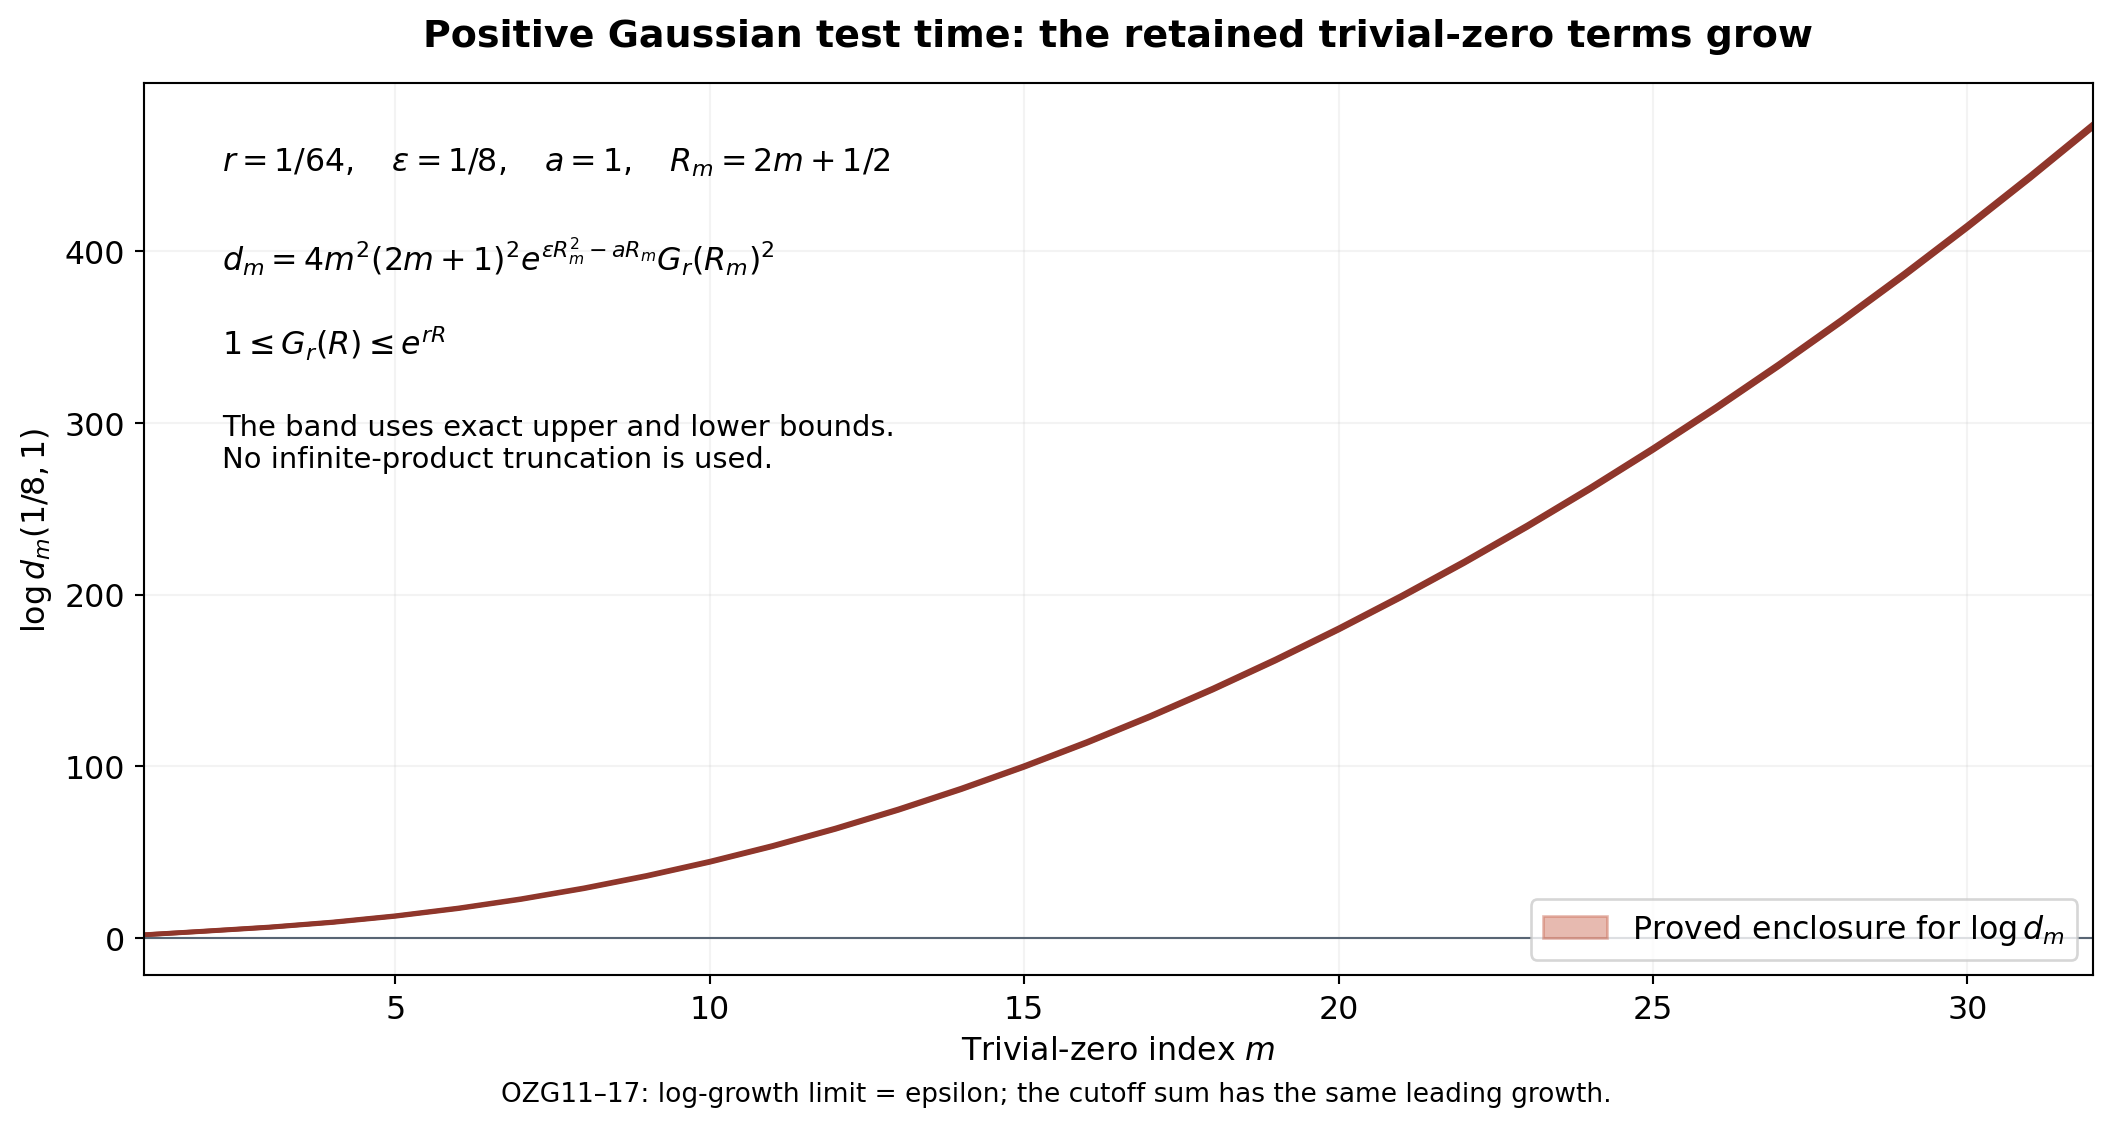
\includegraphics[keepaspectratio,alt={Exact enclosure for the retained trivial-zero terms at the displayed original parameters. The lower and upper edges are the full logarithm of OZG11 with the proved bounds 1 and exp(r R) for G, respectively. OZG13--17 proves divergence and the failure to interchange the positive-time and infinite-cutoff limits. The density is the classical Arias de Reyna function, with the source and exact coordinate comparison stated in OZG3.}]{gaussian_trivial_zero_growth.png}}
\caption{Exact enclosure for the retained trivial-zero terms at the
displayed original parameters. The lower and upper edges are the full
logarithm of OZG11 with the proved bounds 1 and exp(r R) for G,
respectively. OZG13--17 proves divergence and the failure to interchange
the positive-time and infinite-cutoff limits. The density is the
classical Arias de Reyna function, with the source and exact coordinate
comparison stated in OZG3.}
\end{figure}

Pinned public predecessor proofs:
\href{https://github.com/KokunoYumeto/zeta-function-research-reader/blob/a8e35be8f238913ae5bcbd8ad55a07d539b350f3/workbenches/splitzero-tandem/branches/tau-zero-prime-positivity/FAITHFUL_THETA_COMPLETION_RETURN.md\#L149}{Original
theta and its exact return}, TF17;
\href{https://github.com/KokunoYumeto/zeta-function-research-reader/blob/a8e35be8f238913ae5bcbd8ad55a07d539b350f3/workbenches/splitzero-tandem/branches/tau-zero-prime-positivity/FAITHFUL_UNCOMPLETED_ZETA_HEAT.md\#L20}{Original
meromorphic heat family}, UZ1;
\href{https://github.com/KokunoYumeto/zeta-function-research-reader/blob/a8e35be8f238913ae5bcbd8ad55a07d539b350f3/workbenches/splitzero-tandem/branches/tau-zero-prime-positivity/ORIGINAL_ZETA_COMPACT_WEIL_RECONSTRUCTION.md\#L15}{Full
original-zeta contour and compact form}, OZC1;
\href{https://github.com/KokunoYumeto/zeta-function-research-reader/blob/a8e35be8f238913ae5bcbd8ad55a07d539b350f3/workbenches/splitzero-tandem/branches/tau-zero-prime-positivity/ORIGINAL_ZETA_HEAT_CONTACT_RECONSTRUCTION.md\#L17}{Original
heat/contact traces}, OZH1;
\href{https://github.com/KokunoYumeto/zeta-function-research-reader/blob/a8e35be8f238913ae5bcbd8ad55a07d539b350f3/workbenches/splitzero-tandem/branches/tau-zero-prime-positivity/ORIGINAL_ZETA_CAUCHY_RECONSTRUCTION.md\#L184}{Original
Cauchy correction and raw skew defect}, OZK17. Their complete sources
are also retained in this edition. The new full incoming programme TeX
is included above, with its original references and its corrected
receiving maps.

\clearpage

\section{Original zeta under regular affine heat
transport}\label{original-zeta-under-regular-affine-heat-transport}

This proof reconstructs RG1--4, CW1--11 and the marked-unit transport in
the received RECONSTRUCTION.tex using the original meromorphic zeta
family. The map includes the complete ratio of Gamma, endpoint and pi
factors. Its divisor, heat residual, rational trace, exceptional local
units and residue at infinity are calculated separately and retained
together. A quadratic exponential contributes to a
logarithmic-derivative kernel without changing the moving zero divisor.
The exact additional term and its full negative index are proved below.

\subsection{1. Original function and the complete
transport}\label{original-function-and-the-complete-transport}

Fix the factors and connection \[
\begin{aligned}
C(s)&=\tfrac12s(s-1)\pi^{-s/2}\Gamma(s/2),\\
q(s)&=\frac1s+\frac1{s-1}-\frac12\log\pi+\frac12\psi(s/2),\\
\nabla_s&=\partial_s+q(s),\qquad
\mathcal D_C=\tfrac14\nabla_s^2
=\tfrac14\{\partial_s^2+2q\partial_s+q'+q^2\}.
\end{aligned}\tag{OZR1}
\] The original returned heat family from TF/UZ is the meromorphic
function \[
\zeta_\theta(s)=\frac8{C(s)}\int_0^\infty
 e^{\theta u^2}\Phi_G(u)\cosh((2s-1)u)\,du,
\qquad \zeta_0=\zeta.
\tag{OZR2}
\] Here the original Gaussian theta kernel is \[
\Phi_G(u)=\sum_{n\ge1}
 (2\pi^2n^4e^{9u}-3\pi n^2e^{5u})e^{-\pi n^2e^{4u}},
\] with its exact source inverse and constants proved in TF1--42. Its
doubly exponential tail justifies differentiation for finite complex
\(\theta,s\). Differentiating the displayed integrand gives
\(\partial_\theta\zeta_\theta=\mathcal D_C\zeta_\theta\), because the
second derivative of \(\cosh((2s-1)u)\) is \(4u^2\) times that function.
Thus the equation contains every term in (OZR1); it is not the free heat
equation for \(\zeta_\theta\).

For a real parameter \(t\), take real differentiable functions
\(a,b,c,\alpha,y,\theta\), with \(\alpha>0\), and set \[
r=s-\tfrac12,\qquad
\varphi_t(s)=\tfrac12+\alpha r+iy,\qquad
\chi_t(s)=ar^2+ibr+c.
\tag{OZR3}
\] The receiving map on meromorphic functions on \(\mathbb C\) is \[
(\mathcal T_t f)(s)=M_t(s)f(\varphi_t(s)),\qquad
M_t(s)=e^{\chi_t(s)}\frac{C(\varphi_t(s))}{C(s)}.
\tag{OZR4}
\] In full factors the multiplier is \[
M_t(s)=e^{\chi_t(s)}
\frac{\tfrac12\varphi_t(s)(\varphi_t(s)-1)
 \pi^{-\varphi_t(s)/2}\Gamma(\varphi_t(s)/2)}
 {\tfrac12s(s-1)\pi^{-s/2}\Gamma(s/2)}.
\tag{OZR5}
\] These are meromorphic identities, including points at which an
individual numerator or denominator factor vanishes or has a pole. At
fixed \(t\) the inverse is \[
f(z)=e^{-\chi_t(\varphi_t^{-1}(z))}
\frac{C(\varphi_t^{-1}(z))}{C(z)}
(\mathcal T_t f)(\varphi_t^{-1}(z)),\qquad
\varphi_t^{-1}(z)=\tfrac12+\frac{z-\tfrac12-iy}{\alpha}.
\tag{OZR6}
\] Substitution proves both inverse identities on a nonempty regular
open set, and meromorphic continuation proves them everywhere. The map
is a complex-linear bijection, not an asserted algebra homomorphism or
isometry. It restricts to an automorphism of the embedded space
\(C^{-1}\mathcal O(\mathbb C)\): multiplying (OZR4) by the full \(C(s)\)
gives \(e^\chi(Cf)\circ\varphi\), and (OZR6) proves the converse. The
embedding into meromorphic functions remains part of this space.

\subsection{2. Every exceptional order and
unit}\label{every-exceptional-order-and-unit}

Let \(s_0\in\mathbb C\), \(z_0=\varphi_t(s_0)\), and use the original
local coordinates \(x=s-s_0\) and \(h=z-z_0=\alpha x\). Write \[
C(z_0+h)=h^{e_z}b_z(h),\quad
C(s_0+x)=x^{e_s}b_s(x),\quad
f(z_0+h)=h^d u(h),
\tag{OZR7}
\] where \(f\) is not identically zero and all three displayed units are
holomorphic and nonzero at zero. The integers \(d,e_z,e_s\) may be
negative. Direct substitution gives the entire local identity \[
\boxed{(\mathcal T_t f)(s_0+x)=
x^{d+e_z-e_s}\alpha^{d+e_z}
e^{\chi_t(s_0+x)}\frac{b_z(\alpha x)u(\alpha x)}{b_s(x)}.}
\tag{OZR8}
\] Thus the target order is \(d+e_z-e_s\); the source order alone is
insufficient at exceptional points. Every constant, power of \(\alpha\),
and analytic unit survives.

For clarity the actual exceptional units of \(C\) are \[
\begin{aligned}
C(-2m+x)&=x^{-1}b_{-2m}(x),\\
b_{-2m}(x)&=(-1)^m\frac{2m(2m+1)\pi^m}{m!}
\left(1-\frac{x}{2m}\right)\left(1-\frac{x}{2m+1}\right)
\pi^{-x/2}\Gamma(1+x/2)
\prod_{j=1}^m\left(1-\frac{x}{2j}\right)^{-1},\\
C(1+x)&=x\,\tfrac12(1+x)\pi^{-(1+x)/2}\Gamma((1+x)/2),\\
C(x)&=(x-1)\pi^{-x/2}\Gamma(1+x/2).
\end{aligned}\tag{OZR9}
\] The Gamma recurrence
\(\Gamma(1+x/2)=\prod_{j=0}^m(x/2-j)\Gamma(-m+x/2)\) proves the first
two lines after inserting both polynomial factors. The last two follow
directly from the same recurrence. In particular
\(e_{-2m}=-1,e_1=1,e_0=0\). This calculation retains the Gamma pole and
endpoint zero at zero through their exact unit, whose value is \(-1\).

Let \(W(x)=\alpha^{d+e_z}e^{\chi_t(s_0+x)}b_z(\alpha x)/b_s(x)\). If
\(u(h)=\sum u_nh^n\), then its transported unit has coefficients \[
\widetilde u_n=\sum_{j=0}^n W_{n-j}\alpha^ju_j.
\tag{OZR10}
\] Since \(W_0\ne0\), this triangular map is invertible at every finite
order by recursion. Its inverse is the expansion of (OZR6). For every
\(N\ge1\), the exact jet isomorphism is \[
h^d\mathcal O_h/h^{d+N}\mathcal O_h
\longrightarrow
x^{d+e_z-e_s}\mathcal O_x/x^{d+e_z-e_s+N}\mathcal O_x.
\] It is linear over the local-ring identification \(h=\alpha x\). The
target exponent is the one in (OZR8), not a substituted ordinary scalar
fibre.

The logarithmic derivatives of the units satisfy \[
\begin{aligned}
(\log\widetilde u)'(0)
&=\chi_t'(s_0)+\alpha\{(\log b_z)'(0)+(\log u)'(0)\}
 -(\log b_s)'(0),\\
(\log\widetilde u)''(0)
&=2a+\alpha^2\{(\log b_z)''(0)+(\log u)''(0)\}
 -(\log b_s)''(0).
\end{aligned}\tag{OZR11}
\] These follow by differentiating the nonvanishing unit in (OZR8). At
ordinary points of the divisor of \(C\), the two additional second
derivatives are \(\alpha^2q'(z_0)-q'(s_0)\). They cannot be omitted from
the curvature of the original zeta unit.

For an independent integer marking \(n\), put
\(\lambda_n(g)=\operatorname{Res}_{h=0}g(h)/(h^nu(h))\,dh\). Write
\(\chi_t(s_0+x)=\chi_0+\chi_1x+ax^2\). The transported marked functional
is exactly \[
\begin{aligned}
\widetilde\lambda_n(g)=e^{-\chi_0}\alpha^{n-d-e_z-1}
\lambda_n\left(
e^{-\chi_1h/\alpha-ah^2/\alpha^2}
\frac{b_s(h/\alpha)}{b_z(h)}g(h/\alpha)\right).
\end{aligned}\tag{OZR12}
\] Indeed substitute (OZR8)'s unit in the residue and change
\(h=\alpha x\); \(x^{-n}dx=\alpha^{n-1}h^{-n}dh\). Multiplying the
retained \(\alpha^{-d-e_z}\) gives the stated power. The marking \(n\)
is not silently set equal to either source or target valuation.

\subsection{3. The full heat residual and its
clocks}\label{the-full-heat-residual-and-its-clocks}

Allow a source residual
\(R_f=(\partial_\theta-\mathcal D_{C,z})f_\theta\). The identities \[
\nabla_s\mathcal T_t f
=M_t(s)\{\chi_t'(s)f(\varphi_t(s))
+\alpha(\nabla_z f)(\varphi_t(s))\},
\] \[
\begin{aligned}
\nabla_s^2\mathcal T_t f=M_t(s)\{&((\chi_t'(s))^2+\chi_t''(s))f(\varphi_t(s))\\
 &+2\alpha\chi_t'(s)(\nabla_z f)(\varphi_t(s))
 +\alpha^2(\nabla_z^2f)(\varphi_t(s))\}.
\end{aligned}
\tag{OZR13}
\] follow by differentiating all three factors of \(M_t\). In particular
\(M_t'/M_t=\chi_t'+\alpha q(\varphi_t)-q(s)\), which accounts for both
connection terms. The time derivative gives \[
\begin{aligned}
\partial_t\mathcal T_t f_\theta=M_t(s)\{&\theta'(\partial_\theta f)(\theta,\varphi_t(s))\\
 &+\dot\varphi_t(s)(\nabla_z f)(\theta,\varphi_t(s))
 +\dot\chi_t(s)f(\theta,\varphi_t(s))\}.
\end{aligned}
\] Subtracting one quarter of (OZR13) proves \[
\begin{aligned}
M_t^{-1}(\partial_t-\mathcal D_{C,s})\mathcal T_t f_\theta
={}&\theta'R_f
 +\frac{\theta'-\alpha^2}{4}\nabla_z^2 f\\
&+\{(\alpha'-a\alpha)r+i(y'-\alpha b/2)\}\nabla_z f\\
&+\{(a'-a^2)r^2+i(b'-ab)r+c'-a/2+b^2/4\}f,
\end{aligned}\tag{OZR14}
\] where every source term on the right is evaluated at
\((\theta(t),\varphi_t(s))\).

Consequently the exact equations for this map to carry every solution of
the original connected equation to a solution are \[
\theta'=\alpha^2,\quad \alpha'=a\alpha,\quad y'=\alpha b/2,
\quad a'=a^2,\quad b'=ab,\quad c'=a/2-b^2/4.
\tag{OZR15}
\] Sufficiency follows from (OZR14). For necessity take successively the
three meromorphic solutions \(f_\theta=C^{-1}\), \(zC^{-1}\), and
\((z^2+\theta/2)C^{-1}\). Their products by the full \(C\) are the
constant, affine and quadratic caloric polynomials. Substitution forces
respectively the coefficients of \(f,\nabla_z f,\nabla_z^2 f\) to
vanish, and polynomial comparison in \(r\) gives all six equations. No
claim about all source functions lying in the original theta image is
used in this necessity test.

For initial data at \(t=0\), write \(d_t=1-a_0t>0\). The solutions are
\[
\begin{aligned}
a&=a_0/d_t,& b&=b_0/d_t,& \alpha&=\alpha_0/d_t,\\
y&=y_0+\frac{\alpha_0b_0t}{2d_t},&
\theta&=\theta_0+\frac{\alpha_0^2t}{d_t},&
c&=c_0-\tfrac12\log d_t-\frac{b_0^2t}{4d_t}.
\end{aligned}\tag{OZR16}
\] Integrating \(a'=a^2\), then substituting into the equations for
\(b,\alpha\), proves their first three formulas. The identity
\((t/d_t)'=d_t^{-2}\) proves the next two. Differentiating the last
formula gives \(a/2-b^2/4\). These checks prove the solution and its
regular domain. The clock is strictly increasing there; the excluded
point \(d_t=0\) is not identified with an original finite heat time.

Under (OZR15) the residual ratio is \[
\frac{(\partial_t-\mathcal D_C)\mathcal T_t f_\theta}
 {\mathcal T_t f_\theta}
=\alpha^2(R_f/f_\theta)\circ\varphi_t.
\tag{OZR17}
\] If its source germ is the retained contact residual
\(-m(m-1)/(4(z-\rho)^2)+B(z)\), with \(B\) holomorphic as proved for the
modified contact dynamics in BT, substitution gives \[
-\frac{m(m-1)}{4(s-\varphi_t^{-1}\rho)^2}
 +\alpha^2B(\varphi_t(s)).
\tag{OZR18}
\] The factors \(\alpha^2\) and the squared local-coordinate factor
cancel exactly in the principal part. Here \(m\) is the order of the
complete source product \(Cf\). At an exceptional target point it need
not equal the raw target order \(m-e_s\); the connection retains this
difference. This statement transports the specified modified residual;
it does not assign that residual to the unmodified heat solution (OZR2),
whose residual is zero.

\subsection{4. Signed divisor and rational traces, including
collisions}\label{signed-divisor-and-rational-traces-including-collisions}

For real \(\theta\), retain the moving divisor \(D_\theta\) of the
entire product \(C\zeta_\theta\), with its actual multiplicities. The
original heat estimates in UZ/AG give its locally finite zero set and
\(\sum_{\rho\in D_\theta}m_\rho/(1+|\rho|^2)<\infty\). At \(\theta=0\)
it is precisely the nontrivial zeta divisor. Algebra of meromorphic
divisors gives \[
\begin{aligned}
\operatorname{div}\zeta_\theta&=D_\theta-\operatorname{div}C,\\
\operatorname{div}(\mathcal T_t\zeta_\theta)
&=\varphi_t^*\operatorname{div}\zeta_\theta
 +\varphi_t^*\operatorname{div}C-\operatorname{div}C\\
&=\varphi_t^*D_\theta+\sum_{m\ge1}[-2m]-[1].
\end{aligned}\tag{OZR19}
\] All three contributions in the middle line are retained as indexed
divisors. When a pulled moving zero meets a fixed divisor point, their
signed orders add, exactly as in (OZR8). The last line is not a claim
that these component sets are disjoint or that every target trivial-zero
order stays one.

For a rational test \(A(s)=O(s^{-2})\), define
\(\operatorname{FP}_p A=[(s-p)^0]A(s)\). For source tests the poles must
avoid \(D_\theta\). For the target test \(A\) below they must avoid
\(\varphi_t^{-1}(D_\theta)\), equivalently the poles of
\(A\circ\varphi_t^{-1}\) must avoid \(D_\theta\). They may meet the
fixed divisor of \(C\). A finite part is a specified local Laurent
coefficient at such a pole. It is not an ordinary value or a limit in an
external parameter. Put \[
\begin{aligned}
E_C^{\rm fp}(A)&=\operatorname{FP}_1A
 -\sum_{m\ge1}\operatorname{FP}_{-2m}A,\\
R_\theta^{\rm fp}(A)&=\sum_{\rho\in D_\theta}m_\rho A(\rho)
 -E_C^{\rm fp}(A),\\
Q_\theta(A)&=R_\theta^{\rm fp}(A)+E_C^{\rm fp}(A).
\end{aligned}\tag{OZR20}
\] The tails converge absolutely by the displayed zero bound and
\(A(s)=O(s^{-2})\). Only finitely many terms require the finite-part
evaluation. A linear coordinate change \(h=\alpha x\) preserves the
constant Laurent coefficient, because \([x^0]\sum a_j\alpha^jx^j=a_0\).
Therefore (OZR19) proves the exact transport \[
\boxed{\widetilde R^{\rm fp}(A)=
R_\theta^{\rm fp}(A\circ\varphi_t^{-1})
 +E_C^{\rm fp}(A\circ\varphi_t^{-1})-E_C^{\rm fp}(A).}
\tag{OZR21}
\] This formula still applies at fixed-divisor resonances. In its first
two terms the Gamma and original trivial-zero entries are at the
original source points; in the last term they are at the target points.
Keeping this entire tuple and using the inverse affine substitution
gives the inverse comparison. Projection to its sum alone is not the
claimed faithful map.

There is also an explicit logarithmic residue formula. Write \[
\ell_\theta=\zeta_\theta'/\zeta_\theta,\qquad
\widetilde\ell=\chi_t'+\alpha(\ell_\theta+q)\circ\varphi_t-q,
\qquad a_\infty(A)=\lim_{s\to\infty}s^2A(s).
\tag{OZR22}
\] Let \(\mathcal P(A)\) be the finite test-pole set, and \(n_p\) the
total original target order of \(\mathcal T_t\zeta_\theta\). Then \[
\boxed{\widetilde R^{\rm fp}(A)=
-\sum_{p\in\mathcal P(A)}\operatorname{Res}_p(A\widetilde\ell)
 +2a\,a_\infty(A)
 +\sum_{p\in\mathcal P(A)}n_p\operatorname{FP}_p A.}
\tag{OZR23}
\] Here is a direct proof with the exceptional unit terms retained. A
local factor \(f=h^nu(h)\), \(A=\sum A_jh^j\) with pole order \(M\) (and
\(M=0\) when holomorphic), satisfies \[
\operatorname{Res}(Af'/f)=nA_0+
\sum_{j=0}^{M-1}A_{-j-1}[h^j](u'/u).
\tag{OZR24}
\] The source genus-one logarithmic expansion of \(C\zeta_\theta\) and
the full Gamma expansion \[
q(s)=\frac1{s-1}-\frac{\gamma_{\rm E}+\log\pi}{2}
 +\sum_{m\ge1}\left(\frac1{2m}-\frac1{s+2m}\right)
\tag{OZR25}
\] are normally convergent on the finitely many integration circles
after their pole terms there are isolated. Pull them back by
\(\varphi_t\), subtract the second expansion, and retain
\(\chi_t'=2as-a+ib\). For every remaining divisor point \(x\) outside
\(\mathcal P(A)\), the rational function \(A(s)/(s-x)\) has total finite
residue zero, and its test-pole residues sum to \(-A(x)\). If \(x\) lies
in the test-pole set, those test residues include all finite poles and
sum to zero; the last term of (OZR23) restores its prescribed
\(n_x\operatorname{FP}_xA\). Constants multiply \(A\) with total finite
residue zero. Finally \(A(s)\chi_t'(s)=2a\,a_\infty(A)/s+O(s^{-2})\), so
its test-pole residues sum to \(2a\,a_\infty(A)\). This proves exactly
the middle correction and its sign. It avoids applying a genus-one
formula to the quadratically multiplied target, which may have growth of
order two.

\subsection{5. Cauchy kernels and the exact infinity
correction}\label{cauchy-kernels-and-the-exact-infinity-correction}

Use the original reflection \(s^\#=1-\bar s\) and tests \[
F_z(s)=\frac1{s-z},\qquad
A_{z,w}(s)=F_z^\#(s)F_w(s)
=-\frac1{(s-z^\#)(s-w)}.
\tag{OZR26}
\] Choose poles outside the pulled-back moving divisor
\(\varphi_t^{-1}(D_\theta)\) and its reflection. Gamma resonances use
(OZR20). We have \(\varphi_t(s^\#)=\varphi_t(s)^\#\) and
\(\chi_t^\#=\chi_t\), by the stated real parameters. The original
meromorphic family itself has the twisted reflection determined by
\(C\); the untwisted reflected function is its full product
\(C\zeta_\theta\). In particular its logarithmic derivative
\(\ell_\theta+q\) obeys the odd reflected identity. Direct substitution
gives \[
F_z\circ\varphi_t^{-1}=\alpha F_{\varphi_t(z)},\qquad
A_{z,w}\circ\varphi_t^{-1}=\alpha^2A_{\varphi_t(z),\varphi_t(w)}.
\tag{OZR27}
\] The compensated divisor and logarithmic kernels consequently are \[
\begin{aligned}
\widetilde Q_{\rm div}(z,w)
&=\widetilde R^{\rm fp}(A_{z,w})+E_C^{\rm fp}(A_{z,w})
=\alpha^2Q_\theta(\varphi_t(z),\varphi_t(w)),\\
\widetilde Q_{\log}(z,w)
&=\frac{\widetilde\ell(w)+q(w)
 +\overline{\widetilde\ell(z)+q(z)}}{w+\bar z-1}
=\alpha^2Q_\theta(\varphi_t(z),\varphi_t(w))+2a.
\end{aligned}\tag{OZR28}
\] The removable cases of the denominator are interpreted by their
derivatives. The imaginary linear terms cancel, while the two real
quadratic derivatives sum to \(2a(w+\bar z-1)\). Equivalently
\(a_\infty(A_{z,w})=-1\), so (OZR23) subtracts \(2a\) from the
logarithmic kernel to give the divisor kernel. Every term agrees in both
calculations.

The original uncompensated trace is explicitly \[
\widetilde R^{\rm fp}(A_{z,w})=
\alpha^2\{R_\theta^{\rm fp}+E_C^{\rm fp}\}
(A_{\varphi_t(z),\varphi_t(w)})-E_C^{\rm fp}(A_{z,w}).
\tag{OZR29}
\] It is not assigned a Hermitian negative index. At \(t=0\) without
remapping the raw skew defect is already nonzero, as calculated in
OZK17. The compensated divisor kernel, its fixed-divisor correction and
the growth correction are separate entries of the retained comparison.

\subsection{6. Infinity direction and the complete negative
index}\label{infinity-direction-and-the-complete-negative-index}

Let \(\mathcal Z\) be the pulled-back distinct moving zero set, weighted
by \(m_\rho\). Put \(\mathcal H=\ell^2(\mathcal Z,m)\),
\((Jv)(\rho)=v(\rho^\#)\). Reflection preserves multiplicity, so \(J\)
is a bounded self-adjoint involution. The divisor form on rational tests
is \[
\widetilde Q_{\rm div}(F,G)
=\sum_{\rho\in\mathcal Z}m_\rho
 \overline{F(\rho^\#)}G(\rho)
=\langle J\operatorname{ev}F,\operatorname{ev}G\rangle.
\tag{OZR30}
\] Take a real \(\sigma\) outside this discrete set and its reflection
and
\(\mathcal R_\sigma=\operatorname{span}\{(s-\sigma)^{-j-1}:j\ge0\}\).
Every evaluation vector lies in \(\mathcal H\) by the retained zero-tail
bound. Define \(\ell_\infty(F)=\lim_{s\to\infty}sF(s)\). The complete
logarithmic form, extending the Cauchy kernel in (OZR28), is \[
\widetilde Q_{\log}(F,G)=\widetilde Q_{\rm div}(F,G)
 +2a\,\overline{\ell_\infty(F)}\ell_\infty(G).
\tag{OZR31}
\] This is also obtained directly from (OZR23), since
\(a_\infty(F^\#G)=-\overline{\ell_\infty(F)}\ell_\infty(G)\).

The map \(F\mapsto(\ell_\infty(F),\operatorname{ev}F)\) is dense in
\(\mathbb C\oplus\mathcal H\), and its first coordinate can be fixed
exactly. To prove it, suppose \(v\) is orthogonal to all evaluations of
\((s-\sigma)^{-j-1}\) with \(j\ge1\). The function \[
H_v(z)=\sum_{\rho\in\mathcal Z}
 \frac{m_\rho\overline{v(\rho)}}{\rho-z}
\tag{OZR32}
\] converges normally away from \(\mathcal Z\) by Cauchy--Schwarz and
the zero-tail bound. All its positive-order derivatives at \(\sigma\)
vanish. It is constant locally, hence on the connected complement of the
discrete zero set. Its residue at \(\rho\) is
\(-m_\rho\overline{v(\rho)}\), so each coefficient is zero. Thus the
kernel of \(\ell_\infty\) has dense evaluation image. Starting with
\(b/(s-\sigma)\) fixes any desired first coordinate \(b\), and elements
of this kernel approximate any remaining evaluation vector.

Let \(\kappa\) be the number, possibly infinite, of distinct two-point
reflection orbits in \(\mathcal Z\). Each such orbit contributes one
negative direction to \(J\); every fixed point contributes a positive
one. The bounded direct-sum form \((2a)\oplus J\), the preceding density
and finite-dimensional approximation prove \[
\boxed{\operatorname{ind}_-\widetilde Q_{\rm div}=\kappa,
\qquad \operatorname{ind}_-\widetilde Q_{\log}
=\kappa+\mathbf1_{a<0}.}
\tag{OZR33}
\] For completeness, any negative subspace injects into the negative
spectral subspace of the bounded operator, giving the upper bound. Given
a finite negative spectral frame \(U\), approximate it by rational-image
columns \(V\). The Gram error is at most
\(\|A\|(2\|U\|\|V-U\|+\|V-U\|^2)\), where \(A=(2a)\oplus J\). Taking the
error below the strict negative margin preserves that frame. This gives
the lower bound for every finite negative dimension, including the case
of infinite index. The same proof with the first coordinate omitted
gives the divisor assertion. Thus a positive quadratic correction does
not remove an existing off-critical negative direction; a negative
correction adds an independently detected infinity direction. This
statement concerns the complete rational space, not a selected finite
matrix.

\subsection{7. Full support and the receiving arithmetic
identity}\label{full-support-and-the-receiving-arithmetic-identity}

For the original finite bounded distributive lattice \(L\), retain \[
G_L(V)=\{(v,1_L):v\in V\}\cup
 \{(0,\lambda):\lambda\ne1_L\},\qquad
e=(0,1_L),\quad\tau=(0,0_L).
\tag{OZR34}
\] The bijection (OZR4) lifts by \((f,1_L)\mapsto(\mathcal T_tf,1_L)\)
and by fixing every lower carrier point. Its inverse is the lift of
(OZR6). Only top support admits a nonzero carrier amplitude. Independent
function values assigned to lower points are retained in the attached
function space, and are not reinterpreted as nonzero amplitudes in this
carrier. A zero output of a nonzero test functional has its specified
support label; it is not changed to \(\tau\).

Write the previously proved full supported identity as
\(\boldsymbol B_L-\boldsymbol Z_{L,\mathrm{div}}=\boldsymbol D_L\),
where its top spectral coefficient is \(Q_\theta\), and the endpoint,
Gamma and arithmetic terms in \(\boldsymbol D_L\) are all retained.
Under the actual test map (OZR27), pull back every term by the same map.
The raw original target divisor is \[
\boldsymbol R_L=\widetilde{\boldsymbol Z}_{L,\mathrm{div}}
 -E_C^{\rm fp}(A)\mathbf e_{1_L},\qquad
\widetilde{\boldsymbol B}_L-\boldsymbol R_L
=\widetilde{\boldsymbol D}_L+E_C^{\rm fp}(A)\mathbf e_{1_L}.
\tag{OZR35}
\] If the logarithmic kernel is used, retain in addition \[
\widetilde{\boldsymbol Z}_{L,\log}
=\widetilde{\boldsymbol Z}_{L,\mathrm{div}}
 +2a\,\overline{\ell_\infty(F)}\ell_\infty(G)\mathbf e_{1_L},
\] \[
\widetilde{\boldsymbol D}_{L,\log}
=\widetilde{\boldsymbol D}_L
 -2a\,\overline{\ell_\infty(F)}\ell_\infty(G)\mathbf e_{1_L}.
\tag{OZR36}
\] Equations (OZR21), (OZR23), (OZR35) and (OZR36) prove the comparison
with every fixed-divisor, growth and support coordinate. The arithmetic
term here is the complete heat continuation at the actual source time
and the actual transformed test. It is not asserted to equal the
time-zero Euler weights at another time. The coefficient semiring \(S\)
has comparison map \(\mathrm{id}_S\), whose pullback sends each prime
ideal to itself. Separately, (OZR4) acts on the function space and fixes
the label set. No ring-spectrum map is inferred from (OZR4), which was
proved complex-linear.

\subsection{Sources and reconstruction
scope}\label{sources-and-reconstruction-scope}

The received RECONSTRUCTION.tex, RG1--4, CW1--11 and CT1--9, supplies
the specified affine/quadratic class and its earlier entire-function
calculation. Its complete source was read in the intake recorded in
INTAKE\_RECORD.json. The reconstruction above independently
differentiates the complete original-zeta multiplier, proves its
exceptional local maps and residue-at-infinity correction, and retains
the underlying growth estimates through their proved TF/UZ/AG/OZK
sources. The source's elementary heat symmetry is not claimed as new.
The full theta inverse and original heat domain are TF1--42; original
fractional modules and all exceptional units are UZ1--53; finite-part
residue conventions and full Cauchy comparison are OZK1--38, including
OZK33a. These complete sources accompany the cumulative collection. BT's
modified contact residual is used only with its proved scope as
identified in (OZR17)--(OZR18).

At \(t=0,\theta_0=0,a_0=b_0=c_0=y_0=0,\alpha_0=1\), the map is the
identity on the original zeta function and every support label. Other
choices retain their full multiplier, source time and coordinate change.
Nothing here proves positivity of the original compensated arithmetic
form at all tests or proves RH.

\begin{figure}
\centering
\pandocbounded{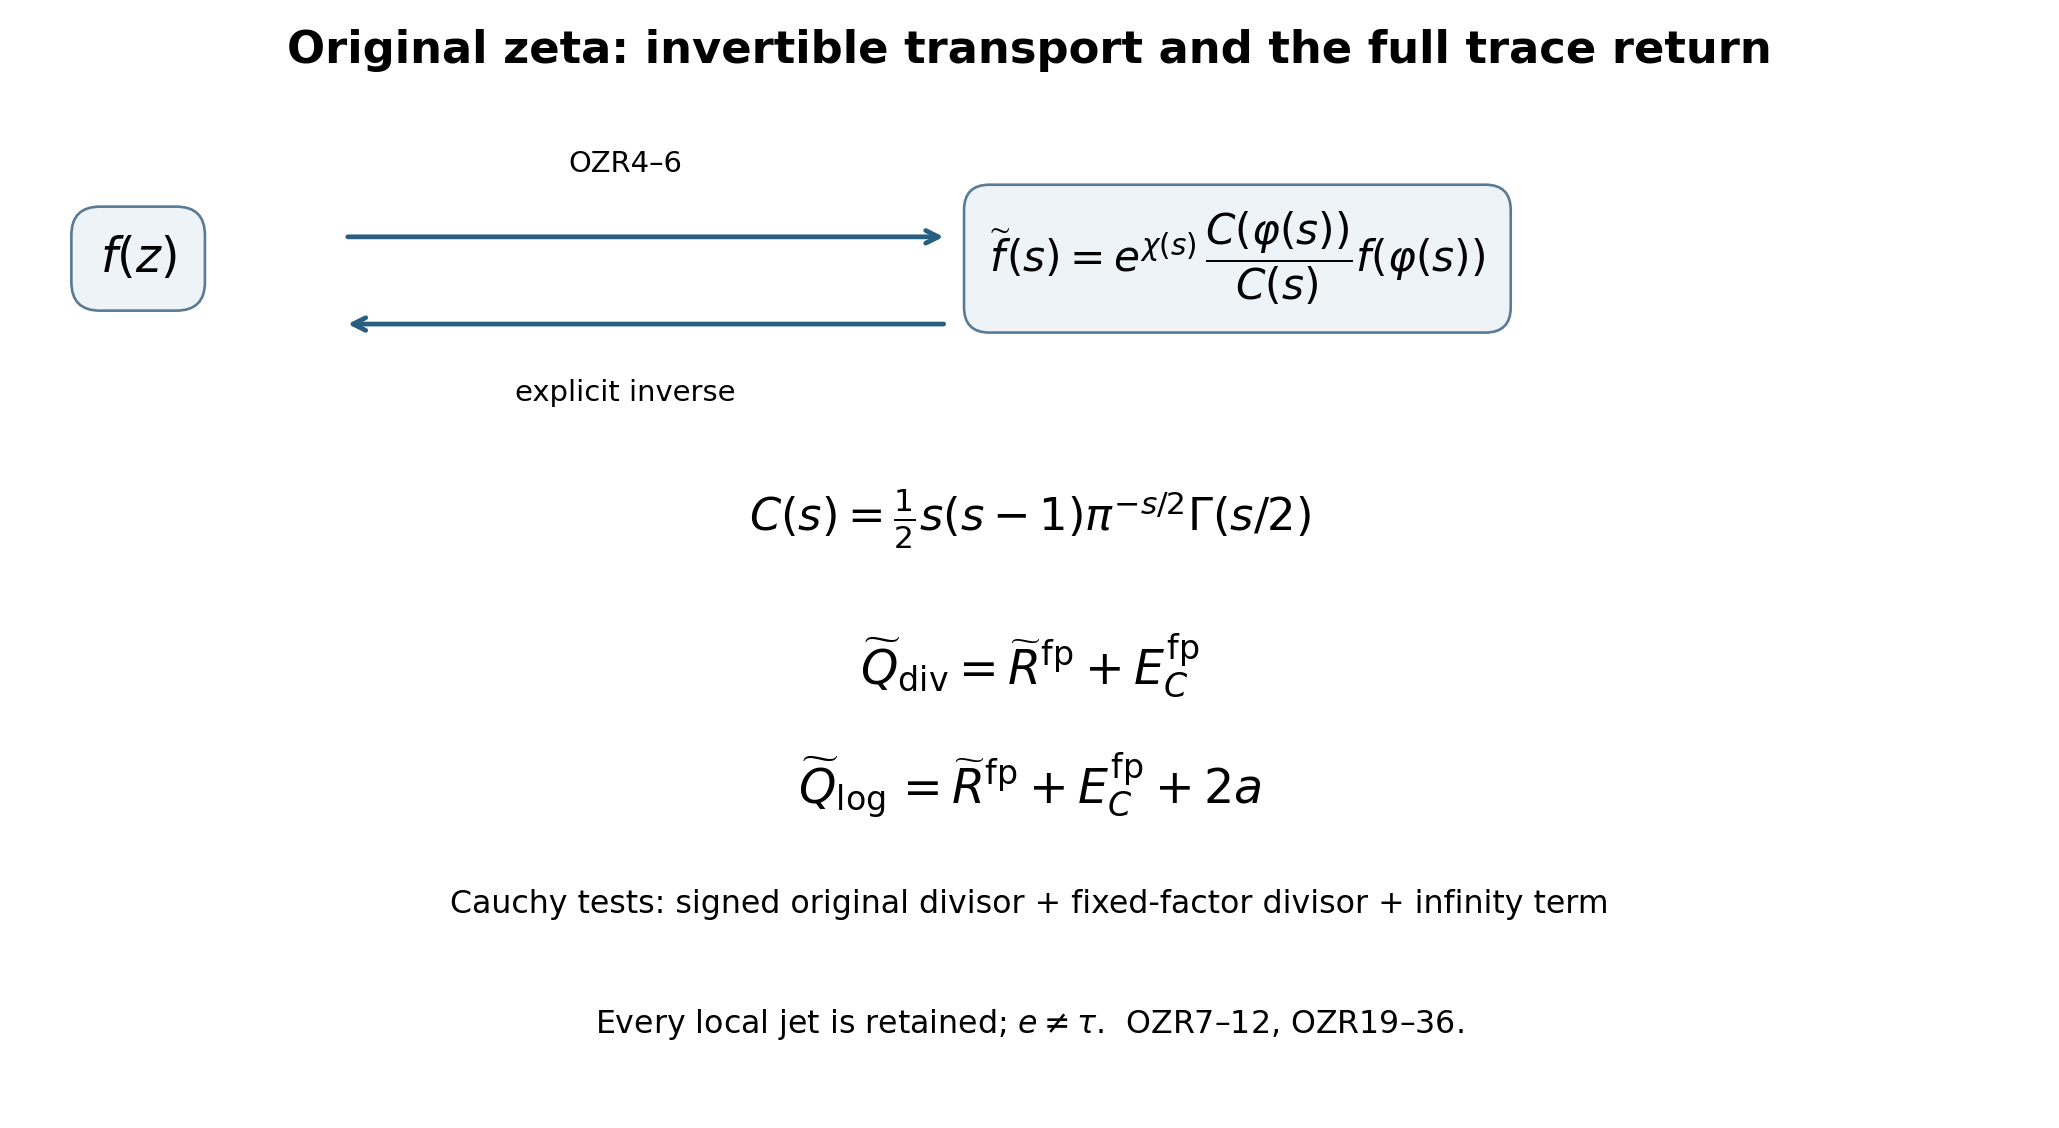
\includegraphics[keepaspectratio,alt={The complete original-zeta map and the exact inverse in OZR4--6 preserve every exceptional valuation and jet by OZR7--12. Here chi(s)=a(s−1/2)\^{}2+ib(s−1/2)+c.~For the Cauchy test the complete signed-divisor trace, fixed-factor trace, and infinity contribution are the three separately retained quantities in OZR19--36. The plus 2a term belongs to the logarithmic kernel. OZR33 proves its full negative-index effect.}]{original_zeta_regular_transport.png}}
\caption{The complete original-zeta map and the exact inverse in OZR4--6
preserve every exceptional valuation and jet by OZR7--12. Here
chi(s)=a(s−1/2)\^{}2+ib(s−1/2)+c.~For the Cauchy test the complete
signed-divisor trace, fixed-factor trace, and infinity contribution are
the three separately retained quantities in OZR19--36. The plus 2a term
belongs to the logarithmic kernel. OZR33 proves its full negative-index
effect.}
\end{figure}

Pinned public predecessor proofs:
\href{https://github.com/KokunoYumeto/zeta-function-research-reader/blob/a8e35be8f238913ae5bcbd8ad55a07d539b350f3/workbenches/splitzero-tandem/branches/tau-zero-prime-positivity/FAITHFUL_THETA_COMPLETION_RETURN.md\#L149}{Original
theta and its exact return}, TF17;
\href{https://github.com/KokunoYumeto/zeta-function-research-reader/blob/a8e35be8f238913ae5bcbd8ad55a07d539b350f3/workbenches/splitzero-tandem/branches/tau-zero-prime-positivity/FAITHFUL_UNCOMPLETED_ZETA_HEAT.md\#L20}{Original
meromorphic heat family}, UZ1;
\href{https://github.com/KokunoYumeto/zeta-function-research-reader/blob/a8e35be8f238913ae5bcbd8ad55a07d539b350f3/workbenches/splitzero-tandem/branches/tau-zero-prime-positivity/ORIGINAL_ZETA_COMPACT_WEIL_RECONSTRUCTION.md\#L15}{Full
original-zeta contour and compact form}, OZC1;
\href{https://github.com/KokunoYumeto/zeta-function-research-reader/blob/a8e35be8f238913ae5bcbd8ad55a07d539b350f3/workbenches/splitzero-tandem/branches/tau-zero-prime-positivity/ORIGINAL_ZETA_HEAT_CONTACT_RECONSTRUCTION.md\#L17}{Original
heat/contact traces}, OZH1;
\href{https://github.com/KokunoYumeto/zeta-function-research-reader/blob/a8e35be8f238913ae5bcbd8ad55a07d539b350f3/workbenches/splitzero-tandem/branches/tau-zero-prime-positivity/ORIGINAL_ZETA_CAUCHY_RECONSTRUCTION.md\#L184}{Original
Cauchy correction and raw skew defect}, OZK17. Their complete sources
are also retained in this edition. The new full incoming programme TeX
is included above, with its original references and its corrected
receiving maps.

\clearpage

\section{Sources, exact proof locations, and reading
scope}\label{sources-exact-proof-locations-and-reading-scope}

This addition develops the established tau/split-zero base, the original
escaping inverse fibre, and the actual quotient-size interpolation.
Every new algebraic and analytic calculation appears in full in the
accompanying complete proof files. The exact operator input retains its
earlier public definitions and proofs; those are linked below. This is
not a historical novelty claim or a proof of the Riemann hypothesis.

\subsection{Earlier programme proofs}\label{earlier-programme-proofs}

\begin{itemize}
\tightlist
\item
  The supported-zero prime and chain are prior programme results. Paper
  1 is \emph{An Algebraic Structure Incorporating a Z/1Z-Symmetric
  Element Adjoined to the Integers: Construction, Analysis, and
  Generalizations}, original \texttt{11.\allowbreak{}tex},
  \href{https://github.com/KokunoYumeto/zeta-function-research-reader/blob/ac168d55cbb400a6c8926a00d67909ba65646ac5/workbenches/splitzero-tandem/branches/identity-absorber-square/sources/17555345_11.tex}{complete
  public source}, labels \texttt{thm:\allowbreak{}prime\_\allowbreak{}ideals\_\allowbreak{}S},
  \texttt{thm:\allowbreak{}krull\_\allowbreak{}dim\_\allowbreak{}S}, \texttt{eq:\allowbreak{}maximal\_\allowbreak{}chain}. The source was
  read completely, 1--1833. The user attributes this result to Gemini
  Pro 2.5; this is received attribution, not an inferred author field.
  The present proof of the full-support statement is
  \href{https://github.com/KokunoYumeto/zeta-function-research-reader/blob/173dbc6ed5a03235dbe7654f928f3692107db39b/workbenches/splitzero-tandem/branches/tau-zero-prime-positivity/FULL_SUPPORT_RECONSTRUCTION_DERIVATION.md}{FSR1--FSR7}.
\item
  \emph{Split Support Geometry: Universal Zero Fibres, Arithmetic
  Curves, and Frobenius-Perfect Quantization}, The Clankers, June 2026,
  version
  \texttt{split\_\allowbreak{}support\_\allowbreak{}geometry\_\allowbreak{}arithmetic\_\allowbreak{}curve\_\allowbreak{}v11910.\allowbreak{}tex},
  SHA256
  \texttt{8443cc04\allowbreak{}01b18d37\allowbreak{}3939d992\allowbreak{}f0a2f538\allowbreak{}4ee2fa11\allowbreak{}30f05975\allowbreak{}3d5f3972\allowbreak{}eec5052d}.
  Root reading covers 1--1910; used definitions and proofs are
  1180--1871. This is the received full-lattice foundation. The complete
  receiving proof, including all needed definitions, is
  \href{https://github.com/KokunoYumeto/zeta-function-research-reader/blob/173dbc6ed5a03235dbe7654f928f3692107db39b/workbenches/splitzero-tandem/branches/tau-zero-prime-positivity/FULL_SUPPORT_RECONSTRUCTION_DERIVATION.md}{FSR1--FSR36},
  not an assertion that the entire source was read.
\item
  The actual escaping map and heat constants are in
  \href{https://github.com/KokunoYumeto/zeta-function-research-reader/blob/ac168d55cbb400a6c8926a00d67909ba65646ac5/satellites/23_source_mechanism_transfer.tex}{Source
  mechanism transfer}, labels \texttt{eq:\allowbreak{}retained-\allowbreak{}node-\allowbreak{}map},
  \texttt{eq:\allowbreak{}retained-\allowbreak{}arithmetic-\allowbreak{}extension}, and
  \href{https://github.com/KokunoYumeto/zeta-function-research-reader/blob/ac168d55cbb400a6c8926a00d67909ba65646ac5/satellites/26_incompressible_fibre_heat.tex}{Incompressible
  fibre heat}, labels \texttt{eq:\allowbreak{}ifh-\allowbreak{}original}, \texttt{eq:\allowbreak{}ifh-\allowbreak{}chart},
  \texttt{eq:\allowbreak{}ifh-\allowbreak{}target-\allowbreak{}flow}, \texttt{eq:\allowbreak{}ifh-\allowbreak{}triple}. Both local source
  versions were read completely; EFI records their exact hashes. The new
  derivation
  \href{https://github.com/KokunoYumeto/zeta-function-research-reader/blob/173dbc6ed5a03235dbe7654f928f3692107db39b/workbenches/splitzero-tandem/branches/tau-zero-prime-positivity/ESCAPING_FIBRE_INFINITESIMAL_DERIVATION.md}{EFI1--EFI68}
  proves every received polynomial identity it uses.
\item
  The original metric and observation are in
  \href{https://github.com/KokunoYumeto/zeta-function-research-reader/blob/5c69161ca70ee187f41df0bfe786e8b6eebed422/workbenches/splitzero-tandem/continuations/20260922-current-effective-cutoff/OBSERVED_CURRENT_PLANE.tex\#L90}{Observed
  current plane}, OCP1 and OCP5--OCP7. Read coverage is 35--169. The
  published exact incoming family and support maps are
  \href{https://github.com/KokunoYumeto/zeta-function-research-reader/blob/4ba9285b66af58a6d58fc502a494c1fb45ca5b79/workbenches/splitzero-tandem/continuations/20260922-support-transport/OBSERVED_DEFORMATION_AND_CURRENT.md\#L22}{Observed
  deformation and current}, DF1--DF16, and
  \href{https://github.com/KokunoYumeto/zeta-function-research-reader/blob/4ba9285b66af58a6d58fc502a494c1fb45ca5b79/workbenches/splitzero-tandem/continuations/20260922-support-transport/SUPPORT_SPECTRUM_AND_TERMINAL_MASS.md}{Support
  spectrum and terminal mass}, ST1--ST20, both read completely and
  byte-matched to their public sources.
\item
  The subsequent complete incoming proofs are
  \href{https://github.com/KokunoYumeto/zeta-function-research-reader/blob/c9df443d9e1df000dfbb083943f97197e746eb08/workbenches/splitzero-tandem/branches/identity-absorber-square/OBSERVED_COLLISION.md}{Observed
  collision}, OC1--OC17;
  \href{https://github.com/KokunoYumeto/zeta-function-research-reader/blob/c9df443d9e1df000dfbb083943f97197e746eb08/workbenches/splitzero-tandem/branches/identity-absorber-square/OBSERVED_SUPPORT_PROPAGATION.md}{Observed
  support propagation}, OSP1--OSP51; and
  \href{https://github.com/KokunoYumeto/zeta-function-research-reader/blob/c9df443d9e1df000dfbb083943f97197e746eb08/workbenches/splitzero-tandem/branches/identity-absorber-square/OBSERVED_COTANGENT_FROBENIUS.md}{Observed
  cotangent and Frobenius}, OCF1--OCF23 and OIF1--OIF36. ISP and EFI
  give the new exact trace/current and escaping-family comparisons.
\end{itemize}

\subsection{Supplied original LaTeX on separated zeta
interpolation}\label{supplied-original-latex-on-separated-zeta-interpolation}

The source-reading ledger is keyed to canonical IDs from the existing
disk index. Its search results were used for routing; they were not
counted as reading.

{\def\LTcaptype{none} % do not increment counter
\begin{longtable}[]{@{}
  >{\raggedright\arraybackslash}p{(\linewidth - 4\tabcolsep) * \real{0.3333}}
  >{\raggedright\arraybackslash}p{(\linewidth - 4\tabcolsep) * \real{0.3333}}
  >{\raggedright\arraybackslash}p{(\linewidth - 4\tabcolsep) * \real{0.3333}}@{}}
\toprule\noalign{}
\begin{minipage}[b]{\linewidth}\raggedright
Source
\end{minipage} & \begin{minipage}[b]{\linewidth}\raggedright
Exact version and root reading
\end{minipage} & \begin{minipage}[b]{\linewidth}\raggedright
Result used here
\end{minipage} \\
\midrule\noalign{}
\endhead
\bottomrule\noalign{}
\endlastfoot
\emph{Secondary Note on Split-Zero Globalization}, The Clankers;
PUBUNIT-B1A260A5E731EA568C353AA4 &
\texttt{split\_\allowbreak{}zero\_\allowbreak{}secondary\_\allowbreak{}note.\allowbreak{}tex}, SHA256
\texttt{8e1aa2f9\allowbreak{}34c49fc2\allowbreak{}1e7a3d94\allowbreak{}6ac6a465\allowbreak{}bc1a6889\allowbreak{}6ec184af\allowbreak{}cb3d989c\allowbreak{}c9f8b364};
complete 1--1997 & \texttt{def:\allowbreak{}hurwitz-\allowbreak{}specialization},
\texttt{thm:\allowbreak{}universal-\allowbreak{}taylor-\allowbreak{}deformation},
\texttt{thm:\allowbreak{}arithmetic-\allowbreak{}kernels-\allowbreak{}riemann},
\texttt{cor:\allowbreak{}first-\allowbreak{}log-\allowbreak{}jet-\allowbreak{}explicit};
\href{https://github.com/KokunoYumeto/zeta-function-research-reader/blob/173dbc6ed5a03235dbe7654f928f3692107db39b/workbenches/splitzero-tandem/branches/tau-zero-prime-positivity/NON_EULERIAN_LENGTH_DERIVATION.md}{NL1--NL18},
\href{https://github.com/KokunoYumeto/zeta-function-research-reader/blob/173dbc6ed5a03235dbe7654f928f3692107db39b/workbenches/splitzero-tandem/branches/tau-zero-prime-positivity/SHIFTED_WEIL_POSITIVITY_DERIVATION.md}{SW1--SW42}
give the complete receiving proofs. \\
\emph{Split-Zero Support Repair}, source author field ``The Clankers /
prepared in continuation''; PUBUNIT-C4735C0E0B05FF5D811C3F89 &
\texttt{some\ considerrations.\allowbreak{}tex}, SHA256
\texttt{3f98c8ea\allowbreak{}b35f8799\allowbreak{}6a594d0a\allowbreak{}fa7d77ba\allowbreak{}561cbc28\allowbreak{}b632fa33\allowbreak{}e16d2d62\allowbreak{}28416702};
1473--1739 & Conservative ideal/zeta side and shifted deformation. The
multiplicative ideal-norm hypothesis is retained explicitly in NL. \\
Split-zero defect preprint, blank source author field;
PUBUNIT-6C3FFDFC49FDF75FE8EB43E3 &
\texttt{split\_\allowbreak{}zero\_\allowbreak{}defect\_\allowbreak{}preprint\ (1).\allowbreak{}tex}, SHA256
\texttt{1d5f15f9\allowbreak{}999b4023\allowbreak{}56d6ba46\allowbreak{}286f2473\allowbreak{}ee6c857f\allowbreak{}55e091c8\allowbreak{}36c905ca\allowbreak{}15b4695e};
480--854 & Endpoint residues and the invariant/anti-invariant
decomposition. SW distinguishes function residues from
logarithmic-derivative multiplicities and derives the reflection
defect. \\
Primitive defect preprint; PUBUNIT-2B18D475F69385B03F1E2B30 &
\texttt{primitive\_\allowbreak{}defect\_\allowbreak{}preprint.\allowbreak{}tex}, SHA256
\texttt{2f3289f6\allowbreak{}a04105d3\allowbreak{}f15fe5f7\allowbreak{}c36dde28\allowbreak{}6515e61f\allowbreak{}465caf15\allowbreak{}82f9808e\allowbreak{}19f3d2f7};
1--385; the two supplied copies are identical & Retained augmentation
kernel; not used as a positivity theorem. \\
Primitive support defects; PUBUNIT-E4607F9536B56699EB520E23 &
\texttt{primitive\_\allowbreak{}support\_\allowbreak{}defects\_\allowbreak{}preprint.\allowbreak{}tex}, SHA256
\texttt{f12f2c1c\allowbreak{}36effbf8\allowbreak{}9740e308\allowbreak{}733d8434\allowbreak{}989e69cc\allowbreak{}088a0fc1\allowbreak{}c686281a\allowbreak{}157b42c5};
1--440 & Source comparison for signed support defects. \\
Split-zero moonshine repair; PUBUNIT-396B23CD772DEC7617B4A2A5 &
\texttt{split\_\allowbreak{}zero\_\allowbreak{}moonshine\_\allowbreak{}repair.\allowbreak{}tex}, SHA256
\texttt{7e672f7f\allowbreak{}1c21ae8d\allowbreak{}ca327a65\allowbreak{}d8395d1a\allowbreak{}8b201bbd\allowbreak{}debb4d03\allowbreak{}17a96ab9\allowbreak{}e2382538};
complete 1--826 & Character-coefficient positivity and retained negative
polar data were read; no moonshine theorem is applied to infer Weil
positivity. \\
\end{longtable}
}

These received manuscripts are identified as programme sources. The
independently written complete receiving proofs are included here. No
private correspondence is reproduced.

\subsection{Human sources}\label{human-sources}

\begin{itemize}
\tightlist
\item
  Alain Connes and Caterina Consani,
  \href{https://arxiv.org/abs/2006.13771v1}{\emph{Weil positivity and
  Trace formula, the archimedean place}, arXiv:2006.13771v1};
  \href{https://arxiv.org/src/2006.13771v1}{original author source
  archive}, \texttt{weil-\allowbreak{}compo.\allowbreak{}tex}, Appendix A ``Fourier versus Mellin
  transforms'' (\texttt{appenmellinapp}) and Appendix B ``Explicit
  formula'' (\texttt{appendix2}), 2011--2070. This exact source block
  was read. Labels \texttt{bombieriexplicit},
  \texttt{bombieriexplicit1}, \texttt{burnolexplicit1} fix the signs and
  conventions. The original archive is retained privately unchanged.
  \href{https://github.com/KokunoYumeto/zeta-function-research-reader/blob/173dbc6ed5a03235dbe7654f928f3692107db39b/workbenches/splitzero-tandem/branches/tau-zero-prime-positivity/WEIL_PACKET_ANALYTIC_DERIVATION.md}{WA1--WA30}
  proves the extension to the actual entire test functions, with
  convergence.
\item
  Terence Tao,
  \href{https://terrytao.wordpress.com/2026/07/21/a-digestion-of-the-jacobian-conjecture-counterexample/}{\emph{A
  digestion of the Jacobian conjecture counterexample}, 21 July 2026},
  displayed original polynomial map; David Speyer,
  \href{https://sbseminar.wordpress.com/2026/07/20/the-new-counterexample-to-the-jacobian-conjecture/}{\emph{The
  new counterexample to the Jacobian conjecture}, 20 July 2026},
  marked-factor discussion, as cited by the programme's source. The
  first displayed map was checked live. Reading those posts does not
  claim a fresh audit of every original counterexample argument.
  EFI1--EFI3 and its exact check script verify the polynomial map and
  its inverse chart directly.
\item
  \href{https://dlmf.nist.gov/25.11}{NIST DLMF, §25.11}, definitions,
  recurrence, special values and parameter derivative, equations
  25.11.1, 25.11.3, 25.11.13, 25.11.14, 25.11.17, were checked in the
  primary HTML. Equation-TeX downloads returned HTTP 403 and the browser
  extractor rejected the TeX content type; no source download is
  claimed, and no PDF was substituted. SW3--SW8 supplies the needed
  continuation and derivative proofs independently.
\end{itemize}

The historical cotangent and prism foundations remain Luc Illusie's
regular-immersion and transitivity theorems and Bhatt--Scholze's prism
definitions, at the exact original-source locators retained in the
linked OCF/OIF paper. This addition proves the specified polynomial and
coefficient maps; it does not assert an unproved equality between
complex Weil pairings and prismatic cohomology.

\subsection{ES and endpoint heat source
use}\label{es-and-endpoint-heat-source-use}

The ES inputs belong to the established Erdős--Straus collection. The
source read is its original TeX, including the raw quarter projectors,
forced metric and tetrahedral actions, original spatial affine map,
simplex linking algebra and free-shell carrier. The new derivations
reproduce every finite matrix and every connecting map they use. They do
not attribute these older ES constructions to this addition.

\href{https://github.com/KokunoYumeto/erdos-straus-foundation/blob/20709bee872ad10e4cc7d7b976d975e24532a803/00_ERDOS_STRAUSS_Project_Reader.pdf}{The
exact 488-page reading edition} is pinned at
\texttt{20709bee\allowbreak{}872ad10e\allowbreak{}4cc7d7b9\allowbreak{}76d975e2\allowbreak{}4532a803}.
\href{https://github.com/KokunoYumeto/erdos-straus-foundation/blob/20709bee872ad10e4cc7d7b976d975e24532a803/01_ERDOS_STRAUSS_Reader_Source_and_Build.zip}{The
original TeX/build ZIP} contains
\texttt{reader/\allowbreak{}erdos\_\allowbreak{}straus\_\allowbreak{}project\_\allowbreak{}reader.\allowbreak{}tex}, SHA256
\texttt{678b3f70\allowbreak{}ee7d2a6d\allowbreak{}00f6c588\allowbreak{}d7778e39\allowbreak{}0118ab47\allowbreak{}43a57596\allowbreak{}12dbba64\allowbreak{}30984c78}.
The intact local archive has SHA256
\texttt{521582fa\allowbreak{}5d25eae3\allowbreak{}ab8771fc\allowbreak{}0668ca52\allowbreak{}374f21ff\allowbreak{}0f8871a7\allowbreak{}2e652aa0\allowbreak{}90849dd8}.
The local PDF was byte-matched to the pinned public Git blob.

Exact reader-source blocks read for this addition are 4981--5121 (raw
quarter spectrum and projectors), 20151--20370 (the full simplex 1--2--3
linking map and its proof), and 23426--23960 (ordered shell blades,
simplex support, directed carrier and complete
control-length/determinant proof). The corresponding labels are
\texttt{cor:\allowbreak{}raw-\allowbreak{}blade-\allowbreak{}cells-\allowbreak{}quarter-\allowbreak{}three-\allowbreak{}plus-\allowbreak{}one},
\texttt{eq:\allowbreak{}raw-\allowbreak{}negative-\allowbreak{}cell-\allowbreak{}projector},
\texttt{thm:\allowbreak{}simplex-\allowbreak{}123-\allowbreak{}modular-\allowbreak{}intertwiner},
\texttt{cor:\allowbreak{}general-\allowbreak{}shell-\allowbreak{}simplex-\allowbreak{}Lorentz-\allowbreak{}pullback}, and
\texttt{thm:\allowbreak{}general-\allowbreak{}shell-\allowbreak{}control-\allowbreak{}determinant-\allowbreak{}volume}. Figures 10 and 12
are the supplied images' linking and shell constructions. Further source
reading in the current ES manuscript covered the exact forced metric, D3
action, regular tetrahedral completion and moving spatial map at the
labels recorded in ESQ. This is bounded reading, not a claim to have
reread the entire collection.

The endpoint convention is the same primary-source explicit formula
already read in Connes--Consani's original author TeX, at the Appendix B
locators above. HEB13--HEB17 prove the exact endpoint isomorphism;
HEB26--HEB30 prove its rational completion correction. The original
polynomial map and heat speed retain the public source-mechanism and
incompressible-fibre citations above. No new claim is made for a global
arithmetic identification of the ES operator or its infinite fibre
trace.

The original eight-state source is
\href{https://github.com/KokunoYumeto/zeta-function-research-reader/blob/0fd693c844aad9117e30ec447c59864a28af10f3/workbenches/splitzero-tandem/continuations/20260921-native-spectral-real-pair/005/independent/FINITE_SIGNED_COMPLETION.tex}{the
finite signed-root completion, FS1--FS31}, read in full. Its source
SHA256 is
\texttt{eaf980a1\allowbreak{}6e7d639e\allowbreak{}21953e57\allowbreak{}79e7f76a\allowbreak{}bf18e8bd\allowbreak{}b80ae923\allowbreak{}c4160b45\allowbreak{}6c22da6f}.
The original polynomial and escaping arcs are
\href{https://github.com/KokunoYumeto/zeta-function-research-reader/blob/ab45e221579a0d48ce2885b4ecdf1a6aefc24a20/workbenches/splitzero-tandem/continuations/20260920-fable-boundary-action/FABLE_TO_ORIGINAL_CONDUCTOR.tex\#L590}{FC36--FC47},
read at public-source lines 590--769, SHA256
\texttt{10906ba3\allowbreak{}bd21c066\allowbreak{}45571560\allowbreak{}e4c7b0c3\allowbreak{}948c0cca\allowbreak{}f65d8b9e\allowbreak{}525abf7c\allowbreak{}d732794c}.
ESH preserves these original constructions and proves the new heat
receivers and whole-fibre trace comparisons.

\subsection{Supported-zero trace and signed-cover
holonomy}\label{supported-zero-trace-and-signed-cover-holonomy}

The supported-zero derivation uses the original author TeX of Alain
Connes, \href{https://arxiv.org/abs/math/9811068v1}{Trace formula in
noncommutative geometry and the zeros of the Riemann zeta function,
arXiv:math/9811068v1}, Section III (two-endpoint function space),
Section VI (formal orbital discussion), Appendix I (full Poisson
formula), and Appendix II Theorem6 (unconditional explicit formula). SZW
derives its stated arithmetic formula by a convergent contour argument
and constructs its separate divisor-jet Hilbert receiver explicitly. It
does not identify that receiver with an unproved global operator trace.
The complete preceding TPS, TC and FL proofs are included in
supporting\_proofs, with original-source identity and exact scope
preserved. Private correspondence is not included.

The actual order-192 monodromy was already proved in
\href{https://github.com/KokunoYumeto/zeta-function-research-reader/blob/ab45e221579a0d48ce2885b4ecdf1a6aefc24a20/workbenches/splitzero-tandem/continuations/20260920-fable-boundary-action/FABLE_TO_ORIGINAL_CONDUCTOR.tex\#L2097}{SM1--SM19,
source lines2097--2513}. The downloaded original has
SHA25610906ba3bd21c06645571560e4c7b0c3948c0ccaf65d8b9e525abf7cd732794c.
Root read that complete section and the full new SZW, EHM and HWA
proofs. Independent mathematical review checked the analytic trace
construction and the complete finite averaging; symbolic checks
supplement, rather than replace, those proofs. EHM derives the new
explicit infinity loop, heat collision maps and nonzero residue in
original coordinates. Figures31--33 display the corresponding proved
maps and were rendered and inspected.

\subsection{Class-field source and precise
application}\label{class-field-source-and-precise-application}

Alain Connes and Caterina Consani,
\href{https://arxiv.org/abs/2501.06560v1}{Knots, primes and class field
theory, arXiv:2501.06560v1}, introductory Theorem1 and original source
labels coverdef, mappingtorus1, artinrec, main. Root read the original
author TeX body and bibliography in full, lines169 through end. The
intact original archive remains preserved; its SHA256
is5c8578f1296d2fc2c1cbf0b98f0692402b84f0b5907e090951ffe27c128cce82, and
arxiv-pisa.tex has
SHA256249fed347469cfaf6da97915d547c2ca704a4ba21cc339613713e570f14d5cea.
The source identity is also recorded in
CONNES\_CLASS\_FIELD\_SOURCE.json.

The source proves a functor from finite abelian extensions to adelic
covers, identifying unramified periodic monodromy with arithmetic
Frobenius. PHW derives the correctly oriented periodic traces, inertia
and fixed-support coefficient maps, and their convergent Euler-contour
calculation. CBR computes the actual signed frame character and its
conductor-23 arithmetic specialization, including the different integral
model at2 and the heat collision residue. The paper is not represented
as proving RH or positivity from nontrivial monodromy. PHW and CBR have
root mathematical review; CBR also has72 exact finite and polynomial
checks. The additional topological specialization-space calculation
remains outside this edition. The integral collision sources are linked
explicitly in DP11; DP, EC and SG now supply the complete
distinguished-prism construction, extension classification and
supported-spectrum maps.

\subsection{Original supported-zero identity, heat source, and residue
duality}\label{original-supported-zero-identity-heat-source-and-residue-duality}

The original programme
\href{supporting_sources/17555345_11.tex\#L1146}{singlet-algebra proof},
theorem thm:structure\_A, was reread at lines1146--1260; the operation
table is at578--625. The intact source has an empty author field and is
retained as an earlier programme source, not attributed to this edition.
The \href{supporting_sources/globalization_note.tex}{globalization
note}, propositions prop:projection-kernel and prop:units-irr and
theorem thm:zero-prime-not-irr, retains both the singlet identity and
ambient unit statements. ZH proves the complete semimodule and heat
comparisons directly.

Brad Rodgers and Terence Tao,
\href{https://arxiv.org/abs/1801.05914v5}{The De Bruijn--Newman constant
is non-negative, arXiv:1801.05914v5}, original fmp-template.tex:
introduction definitions and theorem main, lines64--133, and heat
discussion166--315, were read. Dave Platt and Tim Trudgian,
\href{https://arxiv.org/abs/2004.09765v1}{The Riemann hypothesis is true
up to 3·10¹², arXiv:2004.09765v1}, original source131--159, gives the
stated bound0.2. The source archives remain intact; no full reading of
either verification proof is claimed. ZH uses their exact heat
conventions and HZ proves the local persistence argument itself.

RD proves the integral Frobenius pairings and trace identities in full,
with108 supplementary exact checks. Its actual packet calculation uses
the retained WP multiplier and WA24 analytic formula, with the complete
SZW label-resolved endpoints. Independent mathematical review checked
every RD formula, including the cotangent presentation and signed
residue defect. It does not supply a general positive Weil form or
construct an off-critical zero.

\subsection{Distinguished collision prism and extension
sources}\label{distinguished-collision-prism-and-extension-sources}

Bhargav Bhatt and Peter Scholze,
\href{https://arxiv.org/src/1905.08229v4}{Prisms and Prismatic
Cohomology, arXiv:1905.08229v4, original author TeX}, source labels
DefPrismCat, distinguishedDivide, prismcrit and PrismMapTaut. The exact
source identity, SHA256 and bounded reading coverage are recorded in
DP11. DP proves all specialized prism axioms and the universal quotient
directly. EC proves its extension group and connecting maps; SG proves
every supported prime map. Original archives remain retained in the
source library.

EC, DP and SG were read in full and checked against their generator
formulas. SG received an independent mathematical review. The extension
checker tests all 27 extension classes and their 243-element middle
modules; the quotient checker tests all 81 ring elements and all ring
pairs for its additive and Leibniz identities. These finite checks
supplement the general proofs. The two diagrams preserve exact maps,
signs and coefficients.

\subsection{Actual heat, global divisor trace, and arithmetic
variation}\label{actual-heat-global-divisor-trace-and-arithmetic-variation}

Brad Rodgers and Terence Tao, \emph{The de Bruijn--Newman constant is
non-negative},
\href{https://arxiv.org/src/1801.05914v5}{arXiv:1801.05914v5, original
author TeX}, equations \texttt{hoz}, \texttt{sas}, \texttt{phidef},
\texttt{htdef}, supplies the original heat coordinates. The exact
coordinate factor gives the coefficient 1/4 in the arithmetic variable.
The complete supported formula is SZW19--38 in this reader, with its
human Connes source retained. The new proofs establish the global
rational trace, its arithmetic derivative and higher mixed-prime
coefficients, and the complete matrix criterion directly. Classical
complex-analysis and Schur-transfer methods retain their standard
attribution; no novelty claim for those methods or for an equivalent RH
criterion is made.

The 102 symbolic arithmetic checks verify the coordinate factors,
Cauchy/endpoints identities, Dirichlet convolution coefficients and
multiplicity response. Three high-precision actual-zeta evaluations are
consistency checks, not interval certificates or positivity proofs. The
complete arguments and exact domains are in the four appended proofs.
The reproducible formula diagram records the original constants and
every support coordinate.

\subsection{Classical transfer method and exact reflection-index
continuation}\label{classical-transfer-method-and-exact-reflection-index-continuation}

Ball, Joseph A.; Biswas, Animikh; Fang, Quanlei; ter Horst, Sanne.
\emph{Multivariable generalizations of the Schur class: positive kernel
characterization and transfer function realization}. arXiv:0705.2042v3,
2 November 2007. https://arxiv.org/abs/0705.2042v3 . Original author TeX
inspected, §1, Theorem 1.1, Proposition 1.2 and the proof discussion
through (2) ⇒ (3).

The inspected treatment attributes the scalar positive-kernel
Hilbert-space construction to N. Aronszajn, \emph{Theory of reproducing
kernels}, Transactions of the American Mathematical Society 68 (1950),
337--404. It cites J. A. Ball, \emph{Linear systems, operator model
theory and scattering: multivariable generalizations}, in \emph{Operator
Theory and Its Applications (Winnipeg, MB, 1998)}, Fields Institute
Communications 25, American Mathematical Society, 2000, 151--178, for
the lurking-isometry terminology. These two original works were not
inspected for this repair; this historical attribution is through the
inspected Ball--Biswas--Fang--ter Horst source. No historical novelty
for these classical methods is claimed.

The complete CK proof now has the inspected primary-source attribution
at its point of use. NI1--32 and FJ1--29 give all density, index,
finite-jet and heat-coefficient arguments in full. The companion
original HR, HC and HF TeX files are retained unchanged in this source
package; their coordinate and multiplicity conventions are preserved.
The new finite symbolic checks concern the displayed algebra, not the
sign of an infinite arithmetic form.

\subsection{Complete primitive prime-window
continuation}\label{complete-primitive-prime-window-continuation}

The four new complete proofs are PM, PS, UP and PW, linked in the
reading guide. The original programme
\href{HURWITZ_CYCLOTOMIC_RECEIVER.tex}{Hurwitz operator proof},
HCR1--42, and \href{BOUNDARY_PRIMITIVE_ALL_ZERO_RECEIVER.tex}{primitive
boundary proof}, BPZ1--23, accompany them unchanged. Their authorship
and original citations remain in those sources. The arithmetic input
retains the classical Möbius inversion identity and the original Weil
formula. Connes and Consani's
\href{https://arxiv.org/src/2006.13771v1}{original author source for
Weil positivity at the archimedean place}, Section sectsupport, gives
the historical operator comparison in PS. No priority is claimed for
classical local positivity, infinite convolution bumps, or translation
criteria. The collection's explicit support corrections, complete
derivations and exact arithmetic maps are proved in the displayed
sources. The unresolved prime-window bound is not stated as a proved
inequality.

\subsection{Actual heat trace and contact
continuation}\label{actual-heat-trace-and-contact-continuation}

The complete new proofs GC1--31a, CH1--30 and RT1--30 retain the prior
thirty-four proofs and their hypotheses. The companion
\href{CONTACT_DEFECT_TRACE_VARIATION.tex}{contact proof}, BT1--22, is
included unchanged with its human references. The original author TeX
for \href{https://arxiv.org/src/2005.05142v2}{Alexander Dobner, A proof
of Newman's conjecture for the extended Selberg class,
arXiv:2005.05142v2} was read from the intact author archive retained
privately with its source identity. The archive is available directly
from arXiv; it is not redistributed in this edition. Its theorem
debruijnthm, crediting de Bruijn (1950), is used with the exact original
heat time and coordinate. Reading coverage is recorded in RT's source
section. The full distribution subtraction and convolution are proved in
CH, and RT proves the actual positive-real-time differentiability and
all-order meromorphic maps. The exact contact addition cancels the
multiple-zero splitting term; the unit and inter-zero terms remain.
These are not a proof of the time-zero positivity bound.

\subsection{Classical compact density and the full first-prime
continuation}\label{classical-compact-density-and-the-full-first-prime-continuation}

The compact dyadic density is classical.
\href{https://arxiv.org/abs/1702.05442v1}{Juan Arias de Reyna, An
infinitely differentiable function with compact support: Definition and
properties, arXiv:1702.05442v1}, Theorem 1 and equations (1)--(9), gives
its construction and product-zero multiplicities. UP0 proves the exact
coordinate comparison, with the author's Fourier convention preserved.
Original author TeX lines 1--340, including the complete theorem proof,
were read for this comparison; the work is the author's 2017 English
translation of the 1982 paper. Its introduction credits Jessen and
Wintner (1935); that earlier source is not represented as newly read.
The programme's full proof is retained with this human credit at its
point of use.

The supplied programme manuscript Direct RH continuation: the optimal
packet cost in the full Weil form, dated 23 September 2026, provided the
interval-operator method and the three-quarter support estimate
N48--N52. FC reproduces every argument used and extends the width to
19/25. FW applies the result to the unchanged UP/PW test and proves the
following-gap continuation. PT evaluates and bounds the complete actual
heat derivative, using RT's proved interchange. FP and FPC extend the
actual time-zero bound through log 256, retaining every prime power and
the entire archimedean term. The complete 71-case coefficient table,
exact rational enclosures, reproducible figures and checkers accompany
their full proofs. No global positivity, RH proof or novelty claim about
the classical compact function follows from these finite-interval
results.

\subsection{Original-zeta reconstruction of the retained
receivers}\label{original-zeta-reconstruction-of-the-retained-receivers}

The original author heat formula is Rodgers--Tao arXiv:1801.05914v5,
equations hoz, phidef, htdef, with actual bounded source reading
recorded in TF, UZ and OZH. TF reconstructs the even-Schwartz theta
input, all endpoint values and each fixed support coefficient, and
proves the precise heat return obstruction and its principal-part map.
UZ retains the full Gamma factor, all exceptional-point units and jets,
the original meromorphic heat equation, the signed divisor and every
reflected orientation. OZC starts from the original Euler derivative and
Gaussian Poisson formula, computes the finite left-cutoff Gamma
boundary, reconstructs the interval operator and every retained compact
bound, and calculates the full trivial-zero trace. OZH reconstructs the
rational and compact-test heat trace, the complete contact drift, and
the causal prime/Gamma cross terms. Their full proofs are included in
this reader. These are exact receiving calculations; no claim of global
positivity follows from a finite-interval bound or from cancellation of
a fixed-divisor term.

OZK reconstructs every Cauchy and finite-jet receiver from the original
signed divisor, including the complete Gamma correction and the residue
terms at resonant test poles. Its formulas are proved for the original
coefficient basis; its single-stalk heat matrices explicitly concern
critical-line zeros and real time. The independently reproducible 59
rational/Laurent checks supplement its analytic proof.

The complete public companion FR1--38 source is retained unchanged in
\texttt{supporting\_\allowbreak{}proofs/\allowbreak{}ORIGINAL\_\allowbreak{}ZETA\_\allowbreak{}RETURN\_\allowbreak{}FR.\allowbreak{}tex}, from GitHub
proof pin ec73ac350d0cda3d95c0bd1361bede33166b4d34. Root read it in
full. TF37--42 proves the exact coordinate comparison, both inverse
maps, the factor 32 in the original seminorm, and the ambient
heat-defect map with its full domain. The prime-boundary coordinates are
retained even though the original seminorm vanishes on them.

\subsection{Gaussian translation and regular affine heat
reconstruction}\label{gaussian-translation-and-regular-affine-heat-reconstruction}

The incoming complete programme sources are retained byte-identically as
\href{supporting_proofs/SHIFT_SYNCHRONIZATION_RECONSTRUCTION.tex}{the
full incoming reconstruction} and
\href{supporting_proofs/PRIME_TRANSLATION_EXTENSION.tex}{its Gaussian
extension}. Root read both complete sources; OZG has an independent
complete derivation and audit, while OZR has the complete RHR derivation
and ORA audit. The incoming PWG28 expression B2(1/8) is corrected to
16/e+4; its stated prime-tail bound remains valid. The original human
theta source remains \href{https://arxiv.org/abs/1801.05914}{Rodgers and
Tao, The de Bruijn--Newman constant is non-negative}, v5 equations hoz,
phidef and htdef, through the already read TF/UZ source comparison. The
classical density attribution to Arias de Reyna and the original Connes
explicit-formula source are retained at their exact OZG use. No Gaussian
coordinate change is promoted to an RH sign theorem.

Pinned public predecessor proofs:
\href{https://github.com/KokunoYumeto/zeta-function-research-reader/blob/a8e35be8f238913ae5bcbd8ad55a07d539b350f3/workbenches/splitzero-tandem/branches/tau-zero-prime-positivity/FAITHFUL_THETA_COMPLETION_RETURN.md\#L149}{Original
theta and its exact return}, TF17;
\href{https://github.com/KokunoYumeto/zeta-function-research-reader/blob/a8e35be8f238913ae5bcbd8ad55a07d539b350f3/workbenches/splitzero-tandem/branches/tau-zero-prime-positivity/FAITHFUL_UNCOMPLETED_ZETA_HEAT.md\#L20}{Original
meromorphic heat family}, UZ1;
\href{https://github.com/KokunoYumeto/zeta-function-research-reader/blob/a8e35be8f238913ae5bcbd8ad55a07d539b350f3/workbenches/splitzero-tandem/branches/tau-zero-prime-positivity/ORIGINAL_ZETA_COMPACT_WEIL_RECONSTRUCTION.md\#L15}{Full
original-zeta contour and compact form}, OZC1;
\href{https://github.com/KokunoYumeto/zeta-function-research-reader/blob/a8e35be8f238913ae5bcbd8ad55a07d539b350f3/workbenches/splitzero-tandem/branches/tau-zero-prime-positivity/ORIGINAL_ZETA_HEAT_CONTACT_RECONSTRUCTION.md\#L17}{Original
heat/contact traces}, OZH1;
\href{https://github.com/KokunoYumeto/zeta-function-research-reader/blob/a8e35be8f238913ae5bcbd8ad55a07d539b350f3/workbenches/splitzero-tandem/branches/tau-zero-prime-positivity/ORIGINAL_ZETA_CAUCHY_RECONSTRUCTION.md\#L184}{Original
Cauchy correction and raw skew defect}, OZK17. Their complete sources
are also retained in this edition. The new full incoming programme TeX
is included above, with its original references and its corrected
receiving maps.

\end{document}
